

%!TEX root = /Users/sbogutzky/Entwicklung/projects/bogutzky/repositories/2939413/final-draft.tex
\section{Flow und Laufen (intraindividuell)} 

% (fold)
\label{sec:flow_und_laufen_intraindividuell}

\subsection{Einleitung} 

% (fold)
\label{sub:einleitung_5_1}

Ziel der in diesem Abschnitt beschriebenen Studie war es, zu untersuchen, ob subjektive, durch Experience Sampling erhobene, explizite Flow-Merkmale mit den nachfolgenden Kandidaten für ein implizites Messverfahren des Flow-Erlebens beim Laufen in einem Zusammenhang stehen (Abschnitt~\ref{sec:herangehensweise}, Schritt~2): 
\begin{itemize}
	\item mittlere \ac{HR} 
	\item \acs{RMSSD} der zeitbezogenen statistischen \ac{HRV}-Analyse 
	\item mittlere Doppelschrittfrequenz 
	\item Bewegungsaufwand (Abschnitt~\ref{ssub:der_bewegungsfluss}) oder 
	\item normalisierter Shannon Entropie Index der kardio-lokomotorischen Phasensynchronisation (Abschnitt~\ref{ssub:die_kardio_lokomotorische_phasensynchronisation}) 
\end{itemize}

Die Auswahl der Merkmale begründe ich durch: 
\begin{enumerate}
	\item ihre nachgewiesenen Zusammenhänge zum Flow-Erleben bei Tätigkeiten mit geringer physischer Beanspruchung (Abschnitt~\ref{ssub:kardiovaskulare_messungen}) 
	\item die Praktikabilität bei der Ausführung einer physisch beanspruchenden Tätigkeit 
\end{enumerate}

Im Anschluss (Abschnitt~\ref{sec:herangehensweise}, Schritt~3) untersuche ich das zeitliche Verhalten (Prozess) der impliziten Daten, um Übergänge zwischen \emph{Flow} und \emph{nicht Flow} zu identifizieren.

Aufgrund der durch das \acs{BMBF}-Projekt bereitgestellten Shimmer \acp{IMU}, nutzte ich ein Shimmer \ac{EKG}-Modul, das auf die Hauptplatine einer Shimmer \ac{IMU} aufgesetzt wird. Das Shimmer \ac{EKG}-Modul arbeitet mit der Ableitung nach Einthoven \citep[][S.~85ff.]{Behrends2002}. Es handelt sich um eine bipolare Extremitätenableitung, die man routinemäßig mit drei Elektroden plus einer Erdungselektrode erfasst. Ich platzierte vier konventionelle Einwegelektroden auf der Körperoberfläche und verband sie mit vier Kabelverbindungen mit dem Shimmer \ac{EKG}-Modul wie in Abbildung~\ref{fig:equipment_1} dargestellt. Damit erfasst das Shimmer \ac{EKG}-Modul mit zwei Kanälen die zwei Ableitungen (II-III). Ableitung I berechnete ich, indem ich das Signal von LA-LL von dem Signal von RA-LL subtrahierte. 
\begin{itemize}
	\item Ableitung I: zwischen rechtem und linkem Arm (RA-LA) 
	\item Ableitung II: zwischen rechtem Arm und linkem Bein (RA-LL) 
	\item Ableitung III: zwischen linkem Arm und linkem Bein (LA-LL) 
\end{itemize}

Die Ableitung nach Einthoven dient zur Darstellung von Potenzialänderungen in der Frontalebene und ermöglicht u. a. die Identifikation von Herzschlägen, die wir zur Analyse der \ac{HRV} benötigen.

Wie in Abschnitt~\ref{ssub:kardiovaskulare_messungen} zusammengefasst, handelt es sich bei der \acs{RMSSD} um ein physiologisches Merkmal der zeitbezogenen statistischen \ac{HRV}-Analyse, mit dem \citet{Keller2011} bei einer sitzenden Tätigkeit Zusammenhänge mit Flow-Erleben feststellten. Auf Zusammenhangsanalysen mit frequenzbezogenen \ac{HRV}-Merkmalen verzichtete ich aufgrund der in Abschnitt~\ref{sub:zuordnung} beschriebenen Probleme.

Kinematische Daten maß ich mit den bereitgestellten Shimmer \acp{IMU} und einem zusätzlichen Shimmer Gyro-Modul. Die kinematischen Daten benötigte ich, um einzelne sich wiederholende Bewegungsabläufe der Bewegung zu erkennen und den Bewegungsaufwand zu berechnen. Zusätzliche kinematische Merkmale, die z.~B. Abschnitt~\ref{sub:lauftechnik_detektionstechnologie} beschreibt, berücksichtigte ich nicht.

Die Anordnung des Equipments und die Zuverlässigkeit der Datenaufzeichnung testete ich in Vorab-Tests mit drei Freiwilligen aus der Fakultät 4 der Hochschule Bremen. Für die Vorab-Tests verwendete ich denselben Aufbau des Systems, der bei dieser Studie zum Einsatz kam (Abschnitt~\ref{sub:apparat_5_1}). 
\begin{figure}
	[!htb] \centering 
	\includegraphics[width=1.00 
	\textwidth]{equipment_1} \caption[Equipment (Erste Studie: Laufen)]{Equipment der ersten Studie zum Flow-Erleben beim Laufen} \label{fig:equipment_1} 
\end{figure}

% subsection einleitung (end)
\subsection{Methode} 

% (fold)
\label{sub:methode_5_1}

\citet[][S.~989]{Strohrmann2012} argumentieren, Untersuchungen in Außen-Umgebungen durchzuführen, da sich das Laufen auf einem Laufband von dem Laufen in Außen-Umgebungen in Bezug auf kinematische Merkmale unterscheidet. Aus dem genannten Grund entschied ich mich, die Läufe unter realen Bedingungen durchzuführen. Untersuchungen außerhalb von Laboratorien stellen bei ihrer Durchführung eine Herausforderung dar. Außen-Umgebungen sind in einem hohen Maße veränderlich und kontextsensitive Faktoren als Einflüsse auf Merkmale sind grundsätzlich als gegeben anzunehmen. Gleichwohl sind solche Untersuchungen unerlässlich, um eine realistischere Einschätzung der Nutzung in Außen-Umgebungen zu ermöglichen.

Für die in diesem Abschnitt dokumentierte Studie setzte ich ein Echtzeit-Datenerfassungsverfahren (real-time data capture) ein. Die Datenerfassung umfasst \ac{EKG}-Daten und kinematische Daten sowie Selbstauskünfte durch die \ac{FKS}. Die aufgezeichneten Datenströme eines einzelnen Bewegungsablaufs beim Laufen sind in Abbildung~\ref{fig:rohdaten_1} dargestellt. Der Bewegungsablauf beginnt und endet mit dem mittleren Schwung des rechten Beines (negative Signalspitze der Winkelgeschwindigkeit um die X-Achse). 
\begin{sidewaysfigure}
	\resizebox{1.00 
	\textwidth}{!}{
	
	%
	% Created by tikzDevice version 0.10.1 on 2016-09-19 13:44:36
% !TEX encoding = UTF-8 Unicode
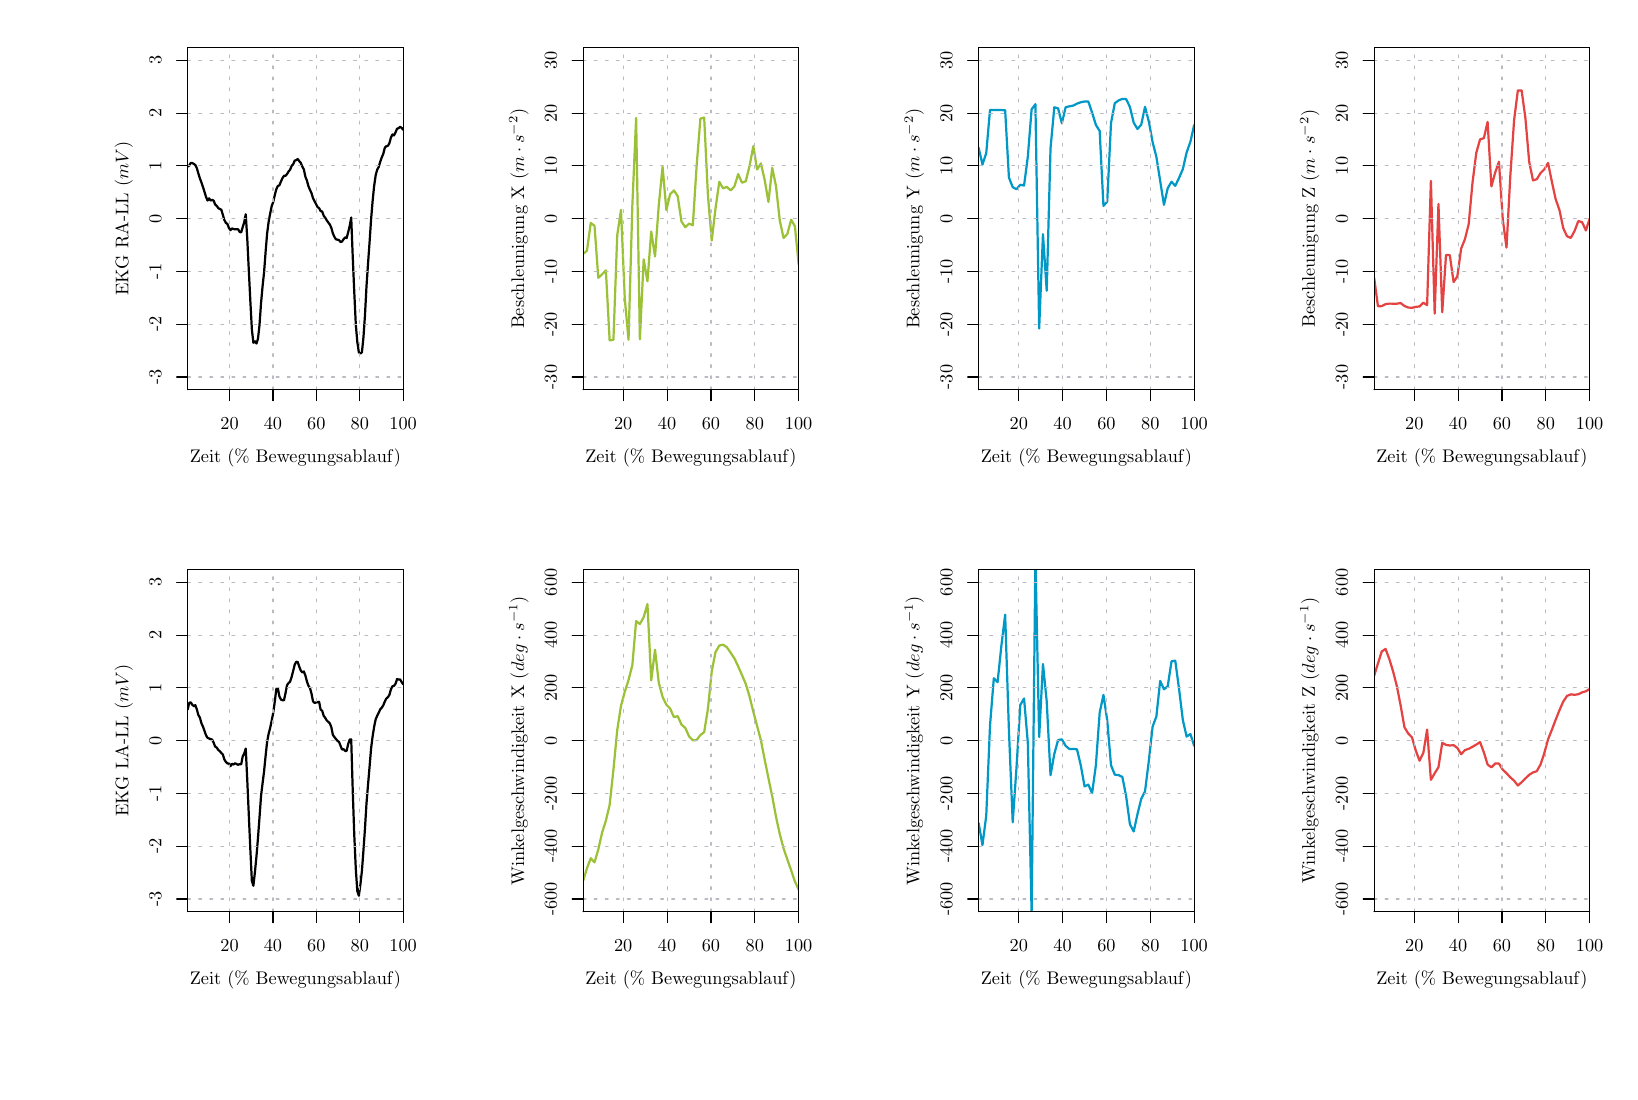
\begin{tikzpicture}[x=1pt,y=1pt]
\definecolor{fillColor}{RGB}{255,255,255}
\path[use as bounding box,fill=fillColor] (0,0) rectangle (571.66,377.25);
\begin{scope}
\path[clip] ( 57.82,246.44) rectangle (135.69,370.02);
\definecolor{drawColor}{RGB}{0,0,0}

\path[draw=drawColor,line width= 0.8pt,line join=round,line cap=round] ( 57.82,327.07) --
	( 58.37,327.42) --
	( 58.92,328.37) --
	( 59.47,328.34) --
	( 60.03,328.02) --
	( 60.58,327.61) --
	( 61.13,326.47) --
	( 61.68,324.55) --
	( 62.23,322.80) --
	( 62.79,321.29) --
	( 63.34,319.69) --
	( 63.89,317.94) --
	( 64.44,316.10) --
	( 65.00,314.78) --
	( 65.55,315.58) --
	( 66.10,314.77) --
	( 66.65,315.02) --
	( 67.20,314.76) --
	( 67.76,313.33) --
	( 68.31,312.86) --
	( 68.86,312.06) --
	( 69.41,311.74) --
	( 69.97,311.49) --
	( 70.52,309.65) --
	( 71.07,307.74) --
	( 71.62,306.71) --
	( 72.18,306.31) --
	( 72.73,304.87) --
	( 73.28,304.08) --
	( 73.83,304.72) --
	( 74.38,304.48) --
	( 74.94,304.40) --
	( 75.49,304.40) --
	( 76.04,304.40) --
	( 76.59,303.44) --
	( 77.15,303.28) --
	( 77.70,305.19) --
	( 78.25,306.94) --
	( 78.80,309.84) --
	( 79.35,300.97) --
	( 79.91,289.48) --
	( 80.46,278.47) --
	( 81.01,268.23) --
	( 81.56,263.38) --
	( 82.12,263.92) --
	( 82.67,263.13) --
	( 83.22,264.83) --
	( 83.77,269.81) --
	( 84.33,277.78) --
	( 84.88,283.80) --
	( 85.43,288.96) --
	( 85.98,296.28) --
	( 86.53,302.94) --
	( 87.09,307.21) --
	( 87.64,310.17) --
	( 88.19,312.82) --
	( 88.74,314.26) --
	( 89.30,316.79) --
	( 89.85,318.89) --
	( 90.40,320.04) --
	( 90.95,320.27) --
	( 91.50,321.60) --
	( 92.06,322.89) --
	( 92.61,323.71) --
	( 93.16,323.72) --
	( 93.71,324.33) --
	( 94.27,325.29) --
	( 94.82,325.92) --
	( 95.37,327.28) --
	( 95.92,327.84) --
	( 96.48,329.20) --
	( 97.03,329.38) --
	( 97.58,329.79) --
	( 98.13,329.02) --
	( 98.68,328.39) --
	( 99.24,327.04) --
	( 99.79,326.04) --
	(100.34,323.42) --
	(100.89,322.03) --
	(101.45,319.98) --
	(102.00,318.66) --
	(102.55,317.49) --
	(103.10,315.65) --
	(103.65,314.58) --
	(104.21,313.48) --
	(104.76,312.41) --
	(105.31,312.02) --
	(105.86,310.98) --
	(106.42,310.83) --
	(106.97,309.27) --
	(107.52,308.58) --
	(108.07,307.65) --
	(108.63,306.83) --
	(109.18,306.13) --
	(109.73,304.91) --
	(110.28,302.91) --
	(110.83,301.67) --
	(111.39,300.76) --
	(111.94,300.64) --
	(112.49,300.52) --
	(113.04,299.80) --
	(113.60,299.96) --
	(114.15,300.82) --
	(114.70,301.45) --
	(115.25,301.22) --
	(115.80,303.29) --
	(116.36,305.59) --
	(116.91,308.64) --
	(117.46,294.43) --
	(118.01,281.80) --
	(118.57,269.92) --
	(119.12,263.62) --
	(119.67,259.93) --
	(120.22,259.45) --
	(120.78,259.95) --
	(121.33,265.34) --
	(121.88,273.27) --
	(122.43,283.79) --
	(122.98,291.89) --
	(123.54,299.70) --
	(124.09,307.90) --
	(124.64,314.58) --
	(125.19,320.03) --
	(125.75,323.95) --
	(126.30,325.93) --
	(126.85,326.95) --
	(127.40,328.81) --
	(127.96,330.39) --
	(128.51,331.69) --
	(129.06,333.87) --
	(129.61,334.43) --
	(130.16,334.53) --
	(130.72,335.53) --
	(131.27,337.59) --
	(131.82,338.65) --
	(132.37,338.31) --
	(132.93,339.44) --
	(133.48,340.74) --
	(134.03,340.94) --
	(134.58,341.42) --
	(135.13,341.04) --
	(135.69,340.33);
\end{scope}
\begin{scope}
\path[clip] (  0.00,  0.00) rectangle (571.66,377.25);
\definecolor{drawColor}{RGB}{0,0,0}

\path[draw=drawColor,line width= 0.4pt,line join=round,line cap=round] ( 72.95,246.44) -- (135.69,246.44);

\path[draw=drawColor,line width= 0.4pt,line join=round,line cap=round] ( 72.95,246.44) -- ( 72.95,242.48);

\path[draw=drawColor,line width= 0.4pt,line join=round,line cap=round] ( 88.63,246.44) -- ( 88.63,242.48);

\path[draw=drawColor,line width= 0.4pt,line join=round,line cap=round] (104.32,246.44) -- (104.32,242.48);

\path[draw=drawColor,line width= 0.4pt,line join=round,line cap=round] (120.00,246.44) -- (120.00,242.48);

\path[draw=drawColor,line width= 0.4pt,line join=round,line cap=round] (135.69,246.44) -- (135.69,242.48);

\node[text=drawColor,anchor=base,inner sep=0pt, outer sep=0pt, scale=  0.66] at ( 72.95,232.18) {20};

\node[text=drawColor,anchor=base,inner sep=0pt, outer sep=0pt, scale=  0.66] at ( 88.63,232.18) {40};

\node[text=drawColor,anchor=base,inner sep=0pt, outer sep=0pt, scale=  0.66] at (104.32,232.18) {60};

\node[text=drawColor,anchor=base,inner sep=0pt, outer sep=0pt, scale=  0.66] at (120.00,232.18) {80};

\node[text=drawColor,anchor=base,inner sep=0pt, outer sep=0pt, scale=  0.66] at (135.69,232.18) {100};

\path[draw=drawColor,line width= 0.4pt,line join=round,line cap=round] ( 57.82,251.02) -- ( 57.82,365.45);

\path[draw=drawColor,line width= 0.4pt,line join=round,line cap=round] ( 57.82,251.02) -- ( 53.86,251.02);

\path[draw=drawColor,line width= 0.4pt,line join=round,line cap=round] ( 57.82,270.09) -- ( 53.86,270.09);

\path[draw=drawColor,line width= 0.4pt,line join=round,line cap=round] ( 57.82,289.16) -- ( 53.86,289.16);

\path[draw=drawColor,line width= 0.4pt,line join=round,line cap=round] ( 57.82,308.23) -- ( 53.86,308.23);

\path[draw=drawColor,line width= 0.4pt,line join=round,line cap=round] ( 57.82,327.30) -- ( 53.86,327.30);

\path[draw=drawColor,line width= 0.4pt,line join=round,line cap=round] ( 57.82,346.37) -- ( 53.86,346.37);

\path[draw=drawColor,line width= 0.4pt,line join=round,line cap=round] ( 57.82,365.45) -- ( 53.86,365.45);

\node[text=drawColor,rotate= 90.00,anchor=base,inner sep=0pt, outer sep=0pt, scale=  0.66] at ( 48.31,251.02) {-3};

\node[text=drawColor,rotate= 90.00,anchor=base,inner sep=0pt, outer sep=0pt, scale=  0.66] at ( 48.31,270.09) {-2};

\node[text=drawColor,rotate= 90.00,anchor=base,inner sep=0pt, outer sep=0pt, scale=  0.66] at ( 48.31,289.16) {-1};

\node[text=drawColor,rotate= 90.00,anchor=base,inner sep=0pt, outer sep=0pt, scale=  0.66] at ( 48.31,308.23) {0};

\node[text=drawColor,rotate= 90.00,anchor=base,inner sep=0pt, outer sep=0pt, scale=  0.66] at ( 48.31,327.30) {1};

\node[text=drawColor,rotate= 90.00,anchor=base,inner sep=0pt, outer sep=0pt, scale=  0.66] at ( 48.31,346.37) {2};

\node[text=drawColor,rotate= 90.00,anchor=base,inner sep=0pt, outer sep=0pt, scale=  0.66] at ( 48.31,365.45) {3};

\path[draw=drawColor,line width= 0.4pt,line join=round,line cap=round] ( 57.82,246.44) --
	(135.69,246.44) --
	(135.69,370.02) --
	( 57.82,370.02) --
	( 57.82,246.44);
\end{scope}
\begin{scope}
\path[clip] (  0.00,188.62) rectangle (142.91,377.25);
\definecolor{drawColor}{RGB}{0,0,0}

\node[text=drawColor,anchor=base,inner sep=0pt, outer sep=0pt, scale=  0.66] at ( 96.75,220.30) {Zeit (\% Bewegungsablauf)};

\node[text=drawColor,rotate= 90.00,anchor=base,inner sep=0pt, outer sep=0pt, scale=  0.66] at ( 36.43,308.23) {EKG RA-LL ($mV$)};
\end{scope}
\begin{scope}
\path[clip] ( 57.82,246.44) rectangle (135.69,370.02);
\definecolor{drawColor}{RGB}{186,187,194}

\path[draw=drawColor,line width= 0.4pt,dash pattern=on 1pt off 3pt ,line join=round,line cap=round] ( 72.95,246.44) -- ( 72.95,370.02);

\path[draw=drawColor,line width= 0.4pt,dash pattern=on 1pt off 3pt ,line join=round,line cap=round] ( 88.63,246.44) -- ( 88.63,370.02);

\path[draw=drawColor,line width= 0.4pt,dash pattern=on 1pt off 3pt ,line join=round,line cap=round] (104.32,246.44) -- (104.32,370.02);

\path[draw=drawColor,line width= 0.4pt,dash pattern=on 1pt off 3pt ,line join=round,line cap=round] (120.00,246.44) -- (120.00,370.02);

\path[draw=drawColor,line width= 0.4pt,dash pattern=on 1pt off 3pt ,line join=round,line cap=round] (135.69,246.44) -- (135.69,370.02);

\path[draw=drawColor,line width= 0.4pt,dash pattern=on 1pt off 3pt ,line join=round,line cap=round] ( 57.82,251.02) -- (135.69,251.02);

\path[draw=drawColor,line width= 0.4pt,dash pattern=on 1pt off 3pt ,line join=round,line cap=round] ( 57.82,270.09) -- (135.69,270.09);

\path[draw=drawColor,line width= 0.4pt,dash pattern=on 1pt off 3pt ,line join=round,line cap=round] ( 57.82,289.16) -- (135.69,289.16);

\path[draw=drawColor,line width= 0.4pt,dash pattern=on 1pt off 3pt ,line join=round,line cap=round] ( 57.82,308.23) -- (135.69,308.23);

\path[draw=drawColor,line width= 0.4pt,dash pattern=on 1pt off 3pt ,line join=round,line cap=round] ( 57.82,327.30) -- (135.69,327.30);

\path[draw=drawColor,line width= 0.4pt,dash pattern=on 1pt off 3pt ,line join=round,line cap=round] ( 57.82,346.37) -- (135.69,346.37);

\path[draw=drawColor,line width= 0.4pt,dash pattern=on 1pt off 3pt ,line join=round,line cap=round] ( 57.82,365.45) -- (135.69,365.45);
\end{scope}
\begin{scope}
\path[clip] (  0.00,  0.00) rectangle (571.66,377.25);
\definecolor{drawColor}{RGB}{0,0,0}

\path[draw=drawColor,line width= 0.4pt,line join=round,line cap=round] ( 57.82,246.44) --
	(135.69,246.44) --
	(135.69,370.02) --
	( 57.82,370.02) --
	( 57.82,246.44);
\end{scope}
\begin{scope}
\path[clip] ( 57.82, 57.82) rectangle (135.69,181.40);
\definecolor{drawColor}{RGB}{0,0,0}

\path[draw=drawColor,line width= 0.8pt,line join=round,line cap=round] ( 57.82,130.89) --
	( 58.37,133.24) --
	( 58.92,133.48) --
	( 59.47,132.59) --
	( 60.03,132.07) --
	( 60.58,132.45) --
	( 61.13,130.89) --
	( 61.68,128.84) --
	( 62.23,127.96) --
	( 62.79,125.87) --
	( 63.34,124.69) --
	( 63.89,123.16) --
	( 64.44,121.58) --
	( 65.00,120.64) --
	( 65.55,120.40) --
	( 66.10,120.16) --
	( 66.65,120.00) --
	( 67.20,118.87) --
	( 67.76,117.44) --
	( 68.31,117.13) --
	( 68.86,116.25) --
	( 69.41,115.85) --
	( 69.97,115.13) --
	( 70.52,114.65) --
	( 71.07,112.81) --
	( 71.62,111.94) --
	( 72.18,111.38) --
	( 72.73,111.38) --
	( 73.28,110.43) --
	( 73.83,111.23) --
	( 74.38,110.98) --
	( 74.94,111.46) --
	( 75.49,111.14) --
	( 76.04,110.90) --
	( 76.59,111.14) --
	( 77.15,111.06) --
	( 77.70,113.93) --
	( 78.25,114.96) --
	( 78.80,116.76) --
	( 79.35,105.33) --
	( 79.91, 92.64) --
	( 80.46, 80.28) --
	( 81.01, 68.90) --
	( 81.56, 67.20) --
	( 82.12, 72.12) --
	( 82.67, 77.77) --
	( 83.22, 84.46) --
	( 83.77, 91.86) --
	( 84.33, 99.71) --
	( 84.88,104.21) --
	( 85.43,108.58) --
	( 85.98,114.15) --
	( 86.53,119.29) --
	( 87.09,122.20) --
	( 87.64,124.27) --
	( 88.19,126.97) --
	( 88.74,129.75) --
	( 89.30,133.78) --
	( 89.85,138.30) --
	( 90.40,138.58) --
	( 90.95,135.64) --
	( 91.50,134.47) --
	( 92.06,134.23) --
	( 92.61,134.18) --
	( 93.16,136.75) --
	( 93.71,139.67) --
	( 94.27,140.44) --
	( 94.82,140.89) --
	( 95.37,142.61) --
	( 95.92,144.75) --
	( 96.48,147.01) --
	( 97.03,148.09) --
	( 97.58,148.07) --
	( 98.13,146.35) --
	( 98.68,144.96) --
	( 99.24,144.27) --
	( 99.79,144.61) --
	(100.34,143.17) --
	(100.89,141.09) --
	(101.45,139.45) --
	(102.00,138.66) --
	(102.55,136.67) --
	(103.10,133.83) --
	(103.65,133.25) --
	(104.21,133.42) --
	(104.76,133.47) --
	(105.31,133.66) --
	(105.86,130.81) --
	(106.42,130.42) --
	(106.97,128.56) --
	(107.52,127.86) --
	(108.07,126.92) --
	(108.63,126.41) --
	(109.18,125.88) --
	(109.73,124.46) --
	(110.28,121.72) --
	(110.83,120.91) --
	(111.39,120.22) --
	(111.94,119.55) --
	(112.49,119.18) --
	(113.04,117.81) --
	(113.60,116.37) --
	(114.15,116.57) --
	(114.70,115.91) --
	(115.25,115.91) --
	(115.80,118.34) --
	(116.36,120.05) --
	(116.91,120.08) --
	(117.46,101.57) --
	(118.01, 85.63) --
	(118.57, 73.15) --
	(119.12, 65.20) --
	(119.67, 63.57) --
	(120.22, 67.56) --
	(120.78, 72.57) --
	(121.33, 79.93) --
	(121.88, 87.83) --
	(122.43, 96.98) --
	(122.98,103.61) --
	(123.54,110.15) --
	(124.09,116.82) --
	(124.64,121.14) --
	(125.19,124.59) --
	(125.75,127.34) --
	(126.30,128.62) --
	(126.85,129.71) --
	(127.40,130.94) --
	(127.96,131.53) --
	(128.51,132.43) --
	(129.06,133.77) --
	(129.61,134.87) --
	(130.16,135.29) --
	(130.72,136.21) --
	(131.27,138.19) --
	(131.82,139.29) --
	(132.37,139.38) --
	(132.93,140.20) --
	(133.48,141.88) --
	(134.03,141.68) --
	(134.58,141.75) --
	(135.13,140.80) --
	(135.69,139.99);
\end{scope}
\begin{scope}
\path[clip] (  0.00,  0.00) rectangle (571.66,377.25);
\definecolor{drawColor}{RGB}{0,0,0}

\path[draw=drawColor,line width= 0.4pt,line join=round,line cap=round] ( 72.95, 57.82) -- (135.69, 57.82);

\path[draw=drawColor,line width= 0.4pt,line join=round,line cap=round] ( 72.95, 57.82) -- ( 72.95, 53.86);

\path[draw=drawColor,line width= 0.4pt,line join=round,line cap=round] ( 88.63, 57.82) -- ( 88.63, 53.86);

\path[draw=drawColor,line width= 0.4pt,line join=round,line cap=round] (104.32, 57.82) -- (104.32, 53.86);

\path[draw=drawColor,line width= 0.4pt,line join=round,line cap=round] (120.00, 57.82) -- (120.00, 53.86);

\path[draw=drawColor,line width= 0.4pt,line join=round,line cap=round] (135.69, 57.82) -- (135.69, 53.86);

\node[text=drawColor,anchor=base,inner sep=0pt, outer sep=0pt, scale=  0.66] at ( 72.95, 43.56) {20};

\node[text=drawColor,anchor=base,inner sep=0pt, outer sep=0pt, scale=  0.66] at ( 88.63, 43.56) {40};

\node[text=drawColor,anchor=base,inner sep=0pt, outer sep=0pt, scale=  0.66] at (104.32, 43.56) {60};

\node[text=drawColor,anchor=base,inner sep=0pt, outer sep=0pt, scale=  0.66] at (120.00, 43.56) {80};

\node[text=drawColor,anchor=base,inner sep=0pt, outer sep=0pt, scale=  0.66] at (135.69, 43.56) {100};

\path[draw=drawColor,line width= 0.4pt,line join=round,line cap=round] ( 57.82, 62.39) -- ( 57.82,176.82);

\path[draw=drawColor,line width= 0.4pt,line join=round,line cap=round] ( 57.82, 62.39) -- ( 53.86, 62.39);

\path[draw=drawColor,line width= 0.4pt,line join=round,line cap=round] ( 57.82, 81.46) -- ( 53.86, 81.46);

\path[draw=drawColor,line width= 0.4pt,line join=round,line cap=round] ( 57.82,100.54) -- ( 53.86,100.54);

\path[draw=drawColor,line width= 0.4pt,line join=round,line cap=round] ( 57.82,119.61) -- ( 53.86,119.61);

\path[draw=drawColor,line width= 0.4pt,line join=round,line cap=round] ( 57.82,138.68) -- ( 53.86,138.68);

\path[draw=drawColor,line width= 0.4pt,line join=round,line cap=round] ( 57.82,157.75) -- ( 53.86,157.75);

\path[draw=drawColor,line width= 0.4pt,line join=round,line cap=round] ( 57.82,176.82) -- ( 53.86,176.82);

\node[text=drawColor,rotate= 90.00,anchor=base,inner sep=0pt, outer sep=0pt, scale=  0.66] at ( 48.31, 62.39) {-3};

\node[text=drawColor,rotate= 90.00,anchor=base,inner sep=0pt, outer sep=0pt, scale=  0.66] at ( 48.31, 81.46) {-2};

\node[text=drawColor,rotate= 90.00,anchor=base,inner sep=0pt, outer sep=0pt, scale=  0.66] at ( 48.31,100.54) {-1};

\node[text=drawColor,rotate= 90.00,anchor=base,inner sep=0pt, outer sep=0pt, scale=  0.66] at ( 48.31,119.61) {0};

\node[text=drawColor,rotate= 90.00,anchor=base,inner sep=0pt, outer sep=0pt, scale=  0.66] at ( 48.31,138.68) {1};

\node[text=drawColor,rotate= 90.00,anchor=base,inner sep=0pt, outer sep=0pt, scale=  0.66] at ( 48.31,157.75) {2};

\node[text=drawColor,rotate= 90.00,anchor=base,inner sep=0pt, outer sep=0pt, scale=  0.66] at ( 48.31,176.82) {3};

\path[draw=drawColor,line width= 0.4pt,line join=round,line cap=round] ( 57.82, 57.82) --
	(135.69, 57.82) --
	(135.69,181.40) --
	( 57.82,181.40) --
	( 57.82, 57.82);
\end{scope}
\begin{scope}
\path[clip] (  0.00,  0.00) rectangle (142.91,188.62);
\definecolor{drawColor}{RGB}{0,0,0}

\node[text=drawColor,anchor=base,inner sep=0pt, outer sep=0pt, scale=  0.66] at ( 96.75, 31.68) {Zeit (\% Bewegungsablauf)};

\node[text=drawColor,rotate= 90.00,anchor=base,inner sep=0pt, outer sep=0pt, scale=  0.66] at ( 36.43,119.61) {EKG LA-LL ($mV$)};
\end{scope}
\begin{scope}
\path[clip] ( 57.82, 57.82) rectangle (135.69,181.40);
\definecolor{drawColor}{RGB}{186,187,194}

\path[draw=drawColor,line width= 0.4pt,dash pattern=on 1pt off 3pt ,line join=round,line cap=round] ( 72.95, 57.82) -- ( 72.95,181.40);

\path[draw=drawColor,line width= 0.4pt,dash pattern=on 1pt off 3pt ,line join=round,line cap=round] ( 88.63, 57.82) -- ( 88.63,181.40);

\path[draw=drawColor,line width= 0.4pt,dash pattern=on 1pt off 3pt ,line join=round,line cap=round] (104.32, 57.82) -- (104.32,181.40);

\path[draw=drawColor,line width= 0.4pt,dash pattern=on 1pt off 3pt ,line join=round,line cap=round] (120.00, 57.82) -- (120.00,181.40);

\path[draw=drawColor,line width= 0.4pt,dash pattern=on 1pt off 3pt ,line join=round,line cap=round] (135.69, 57.82) -- (135.69,181.40);

\path[draw=drawColor,line width= 0.4pt,dash pattern=on 1pt off 3pt ,line join=round,line cap=round] ( 57.82, 62.39) -- (135.69, 62.39);

\path[draw=drawColor,line width= 0.4pt,dash pattern=on 1pt off 3pt ,line join=round,line cap=round] ( 57.82, 81.46) -- (135.69, 81.46);

\path[draw=drawColor,line width= 0.4pt,dash pattern=on 1pt off 3pt ,line join=round,line cap=round] ( 57.82,100.54) -- (135.69,100.54);

\path[draw=drawColor,line width= 0.4pt,dash pattern=on 1pt off 3pt ,line join=round,line cap=round] ( 57.82,119.61) -- (135.69,119.61);

\path[draw=drawColor,line width= 0.4pt,dash pattern=on 1pt off 3pt ,line join=round,line cap=round] ( 57.82,138.68) -- (135.69,138.68);

\path[draw=drawColor,line width= 0.4pt,dash pattern=on 1pt off 3pt ,line join=round,line cap=round] ( 57.82,157.75) -- (135.69,157.75);

\path[draw=drawColor,line width= 0.4pt,dash pattern=on 1pt off 3pt ,line join=round,line cap=round] ( 57.82,176.82) -- (135.69,176.82);
\end{scope}
\begin{scope}
\path[clip] (  0.00,  0.00) rectangle (571.66,377.25);
\definecolor{drawColor}{RGB}{0,0,0}

\path[draw=drawColor,line width= 0.4pt,line join=round,line cap=round] ( 57.82, 57.82) --
	(135.69, 57.82) --
	(135.69,181.40) --
	( 57.82,181.40) --
	( 57.82, 57.82);
\end{scope}
\begin{scope}
\path[clip] (200.73,246.44) rectangle (278.60,370.02);
\definecolor{drawColor}{RGB}{155,193,54}

\path[draw=drawColor,line width= 0.8pt,line join=round,line cap=round] (200.73,295.52) --
	(202.10,296.65) --
	(203.46,306.70) --
	(204.83,305.64) --
	(206.19,286.85) --
	(207.56,288.12) --
	(208.93,289.55) --
	(210.29,264.25) --
	(211.66,264.48) --
	(213.03,302.21) --
	(214.39,311.42) --
	(215.76,279.32) --
	(217.12,264.49) --
	(218.49,312.79) --
	(219.86,344.63) --
	(221.22,264.65) --
	(222.59,293.52) --
	(223.95,285.57) --
	(225.32,303.56) --
	(226.69,294.56) --
	(228.05,313.16) --
	(229.42,326.99) --
	(230.79,311.33) --
	(232.15,317.08) --
	(233.52,318.44) --
	(234.88,316.37) --
	(236.25,307.17) --
	(237.62,305.13) --
	(238.98,306.45) --
	(240.35,305.85) --
	(241.71,327.13) --
	(243.08,344.36) --
	(244.45,344.77) --
	(245.81,316.66) --
	(247.18,300.32) --
	(248.55,311.89) --
	(249.91,321.56) --
	(251.28,319.19) --
	(252.64,319.72) --
	(254.01,318.43) --
	(255.38,319.87) --
	(256.74,324.34) --
	(258.11,321.22) --
	(259.47,321.76) --
	(260.84,327.24) --
	(262.21,334.42) --
	(263.57,325.98) --
	(264.94,328.21) --
	(266.31,322.23) --
	(267.67,314.27) --
	(269.04,326.62) --
	(270.40,319.99) --
	(271.77,307.55) --
	(273.14,301.25) --
	(274.50,302.68) --
	(275.87,307.86) --
	(277.23,305.53) --
	(278.60,291.62);
\end{scope}
\begin{scope}
\path[clip] (  0.00,  0.00) rectangle (571.66,377.25);
\definecolor{drawColor}{RGB}{0,0,0}

\path[draw=drawColor,line width= 0.4pt,line join=round,line cap=round] (215.21,246.44) -- (278.60,246.44);

\path[draw=drawColor,line width= 0.4pt,line join=round,line cap=round] (215.21,246.44) -- (215.21,242.48);

\path[draw=drawColor,line width= 0.4pt,line join=round,line cap=round] (231.06,246.44) -- (231.06,242.48);

\path[draw=drawColor,line width= 0.4pt,line join=round,line cap=round] (246.91,246.44) -- (246.91,242.48);

\path[draw=drawColor,line width= 0.4pt,line join=round,line cap=round] (262.75,246.44) -- (262.75,242.48);

\path[draw=drawColor,line width= 0.4pt,line join=round,line cap=round] (278.60,246.44) -- (278.60,242.48);

\node[text=drawColor,anchor=base,inner sep=0pt, outer sep=0pt, scale=  0.66] at (215.21,232.18) {20};

\node[text=drawColor,anchor=base,inner sep=0pt, outer sep=0pt, scale=  0.66] at (231.06,232.18) {40};

\node[text=drawColor,anchor=base,inner sep=0pt, outer sep=0pt, scale=  0.66] at (246.91,232.18) {60};

\node[text=drawColor,anchor=base,inner sep=0pt, outer sep=0pt, scale=  0.66] at (262.75,232.18) {80};

\node[text=drawColor,anchor=base,inner sep=0pt, outer sep=0pt, scale=  0.66] at (278.60,232.18) {100};

\path[draw=drawColor,line width= 0.4pt,line join=round,line cap=round] (200.73,251.02) -- (200.73,365.45);

\path[draw=drawColor,line width= 0.4pt,line join=round,line cap=round] (200.73,251.02) -- (196.77,251.02);

\path[draw=drawColor,line width= 0.4pt,line join=round,line cap=round] (200.73,270.09) -- (196.77,270.09);

\path[draw=drawColor,line width= 0.4pt,line join=round,line cap=round] (200.73,289.16) -- (196.77,289.16);

\path[draw=drawColor,line width= 0.4pt,line join=round,line cap=round] (200.73,308.23) -- (196.77,308.23);

\path[draw=drawColor,line width= 0.4pt,line join=round,line cap=round] (200.73,327.30) -- (196.77,327.30);

\path[draw=drawColor,line width= 0.4pt,line join=round,line cap=round] (200.73,346.37) -- (196.77,346.37);

\path[draw=drawColor,line width= 0.4pt,line join=round,line cap=round] (200.73,365.45) -- (196.77,365.45);

\node[text=drawColor,rotate= 90.00,anchor=base,inner sep=0pt, outer sep=0pt, scale=  0.66] at (191.23,251.02) {-30};

\node[text=drawColor,rotate= 90.00,anchor=base,inner sep=0pt, outer sep=0pt, scale=  0.66] at (191.23,270.09) {-20};

\node[text=drawColor,rotate= 90.00,anchor=base,inner sep=0pt, outer sep=0pt, scale=  0.66] at (191.23,289.16) {-10};

\node[text=drawColor,rotate= 90.00,anchor=base,inner sep=0pt, outer sep=0pt, scale=  0.66] at (191.23,308.23) {0};

\node[text=drawColor,rotate= 90.00,anchor=base,inner sep=0pt, outer sep=0pt, scale=  0.66] at (191.23,327.30) {10};

\node[text=drawColor,rotate= 90.00,anchor=base,inner sep=0pt, outer sep=0pt, scale=  0.66] at (191.23,346.37) {20};

\node[text=drawColor,rotate= 90.00,anchor=base,inner sep=0pt, outer sep=0pt, scale=  0.66] at (191.23,365.45) {30};

\path[draw=drawColor,line width= 0.4pt,line join=round,line cap=round] (200.73,246.44) --
	(278.60,246.44) --
	(278.60,370.02) --
	(200.73,370.02) --
	(200.73,246.44);
\end{scope}
\begin{scope}
\path[clip] (142.91,188.62) rectangle (285.83,377.25);
\definecolor{drawColor}{RGB}{0,0,0}

\node[text=drawColor,anchor=base,inner sep=0pt, outer sep=0pt, scale=  0.66] at (239.67,220.30) {Zeit (\% Bewegungsablauf)};

\node[text=drawColor,rotate= 90.00,anchor=base,inner sep=0pt, outer sep=0pt, scale=  0.66] at (179.35,308.23) {Beschleunigung X ($m \cdot s^{-2}$)};
\end{scope}
\begin{scope}
\path[clip] (200.73,246.44) rectangle (278.60,370.02);
\definecolor{drawColor}{RGB}{186,187,194}

\path[draw=drawColor,line width= 0.4pt,dash pattern=on 1pt off 3pt ,line join=round,line cap=round] (215.21,246.44) -- (215.21,370.02);

\path[draw=drawColor,line width= 0.4pt,dash pattern=on 1pt off 3pt ,line join=round,line cap=round] (231.06,246.44) -- (231.06,370.02);

\path[draw=drawColor,line width= 0.4pt,dash pattern=on 1pt off 3pt ,line join=round,line cap=round] (246.91,246.44) -- (246.91,370.02);

\path[draw=drawColor,line width= 0.4pt,dash pattern=on 1pt off 3pt ,line join=round,line cap=round] (262.75,246.44) -- (262.75,370.02);

\path[draw=drawColor,line width= 0.4pt,dash pattern=on 1pt off 3pt ,line join=round,line cap=round] (278.60,246.44) -- (278.60,370.02);

\path[draw=drawColor,line width= 0.4pt,dash pattern=on 1pt off 3pt ,line join=round,line cap=round] (200.73,251.02) -- (278.60,251.02);

\path[draw=drawColor,line width= 0.4pt,dash pattern=on 1pt off 3pt ,line join=round,line cap=round] (200.73,270.09) -- (278.60,270.09);

\path[draw=drawColor,line width= 0.4pt,dash pattern=on 1pt off 3pt ,line join=round,line cap=round] (200.73,289.16) -- (278.60,289.16);

\path[draw=drawColor,line width= 0.4pt,dash pattern=on 1pt off 3pt ,line join=round,line cap=round] (200.73,308.23) -- (278.60,308.23);

\path[draw=drawColor,line width= 0.4pt,dash pattern=on 1pt off 3pt ,line join=round,line cap=round] (200.73,327.30) -- (278.60,327.30);

\path[draw=drawColor,line width= 0.4pt,dash pattern=on 1pt off 3pt ,line join=round,line cap=round] (200.73,346.37) -- (278.60,346.37);

\path[draw=drawColor,line width= 0.4pt,dash pattern=on 1pt off 3pt ,line join=round,line cap=round] (200.73,365.45) -- (278.60,365.45);
\end{scope}
\begin{scope}
\path[clip] (  0.00,  0.00) rectangle (571.66,377.25);
\definecolor{drawColor}{RGB}{0,0,0}

\path[draw=drawColor,line width= 0.4pt,line join=round,line cap=round] (200.73,246.44) --
	(278.60,246.44) --
	(278.60,370.02) --
	(200.73,370.02) --
	(200.73,246.44);
\end{scope}
\begin{scope}
\path[clip] (200.73, 57.82) rectangle (278.60,181.40);
\definecolor{drawColor}{RGB}{155,193,54}

\path[draw=drawColor,line width= 0.8pt,line join=round,line cap=round] (200.73, 69.05) --
	(202.10, 73.49) --
	(203.46, 77.13) --
	(204.83, 75.64) --
	(206.19, 80.29) --
	(207.56, 86.35) --
	(208.93, 90.69) --
	(210.29, 96.37) --
	(211.66,109.13) --
	(213.03,123.39) --
	(214.39,132.19) --
	(215.76,137.26) --
	(217.12,141.52) --
	(218.49,146.86) --
	(219.86,162.81) --
	(221.22,161.77) --
	(222.59,164.23) --
	(223.95,168.95) --
	(225.32,141.38) --
	(226.69,152.48) --
	(228.05,140.52) --
	(229.42,135.42) --
	(230.79,132.58) --
	(232.15,131.22) --
	(233.52,128.10) --
	(234.88,128.48) --
	(236.25,125.43) --
	(237.62,124.22) --
	(238.98,121.17) --
	(240.35,119.75) --
	(241.71,119.81) --
	(243.08,121.65) --
	(244.45,122.69) --
	(245.81,131.12) --
	(247.18,144.64) --
	(248.55,151.61) --
	(249.91,153.97) --
	(251.28,154.28) --
	(252.64,153.38) --
	(254.01,151.40) --
	(255.38,149.32) --
	(256.74,146.45) --
	(258.11,143.32) --
	(259.47,140.13) --
	(260.84,135.63) --
	(262.21,130.04) --
	(263.57,124.98) --
	(264.94,119.78) --
	(266.31,112.78) --
	(267.67,106.08) --
	(269.04, 99.50) --
	(270.40, 92.14) --
	(271.77, 85.83) --
	(273.14, 80.70) --
	(274.50, 76.68) --
	(275.87, 72.80) --
	(277.23, 68.74) --
	(278.60, 65.76);
\end{scope}
\begin{scope}
\path[clip] (  0.00,  0.00) rectangle (571.66,377.25);
\definecolor{drawColor}{RGB}{0,0,0}

\path[draw=drawColor,line width= 0.4pt,line join=round,line cap=round] (215.21, 57.82) -- (278.60, 57.82);

\path[draw=drawColor,line width= 0.4pt,line join=round,line cap=round] (215.21, 57.82) -- (215.21, 53.86);

\path[draw=drawColor,line width= 0.4pt,line join=round,line cap=round] (231.06, 57.82) -- (231.06, 53.86);

\path[draw=drawColor,line width= 0.4pt,line join=round,line cap=round] (246.91, 57.82) -- (246.91, 53.86);

\path[draw=drawColor,line width= 0.4pt,line join=round,line cap=round] (262.75, 57.82) -- (262.75, 53.86);

\path[draw=drawColor,line width= 0.4pt,line join=round,line cap=round] (278.60, 57.82) -- (278.60, 53.86);

\node[text=drawColor,anchor=base,inner sep=0pt, outer sep=0pt, scale=  0.66] at (215.21, 43.56) {20};

\node[text=drawColor,anchor=base,inner sep=0pt, outer sep=0pt, scale=  0.66] at (231.06, 43.56) {40};

\node[text=drawColor,anchor=base,inner sep=0pt, outer sep=0pt, scale=  0.66] at (246.91, 43.56) {60};

\node[text=drawColor,anchor=base,inner sep=0pt, outer sep=0pt, scale=  0.66] at (262.75, 43.56) {80};

\node[text=drawColor,anchor=base,inner sep=0pt, outer sep=0pt, scale=  0.66] at (278.60, 43.56) {100};

\path[draw=drawColor,line width= 0.4pt,line join=round,line cap=round] (200.73, 62.39) -- (200.73,176.82);

\path[draw=drawColor,line width= 0.4pt,line join=round,line cap=round] (200.73, 62.39) -- (196.77, 62.39);

\path[draw=drawColor,line width= 0.4pt,line join=round,line cap=round] (200.73, 81.46) -- (196.77, 81.46);

\path[draw=drawColor,line width= 0.4pt,line join=round,line cap=round] (200.73,100.54) -- (196.77,100.54);

\path[draw=drawColor,line width= 0.4pt,line join=round,line cap=round] (200.73,119.61) -- (196.77,119.61);

\path[draw=drawColor,line width= 0.4pt,line join=round,line cap=round] (200.73,138.68) -- (196.77,138.68);

\path[draw=drawColor,line width= 0.4pt,line join=round,line cap=round] (200.73,157.75) -- (196.77,157.75);

\path[draw=drawColor,line width= 0.4pt,line join=round,line cap=round] (200.73,176.82) -- (196.77,176.82);

\node[text=drawColor,rotate= 90.00,anchor=base,inner sep=0pt, outer sep=0pt, scale=  0.66] at (191.23, 62.39) {-600};

\node[text=drawColor,rotate= 90.00,anchor=base,inner sep=0pt, outer sep=0pt, scale=  0.66] at (191.23, 81.46) {-400};

\node[text=drawColor,rotate= 90.00,anchor=base,inner sep=0pt, outer sep=0pt, scale=  0.66] at (191.23,100.54) {-200};

\node[text=drawColor,rotate= 90.00,anchor=base,inner sep=0pt, outer sep=0pt, scale=  0.66] at (191.23,119.61) {0};

\node[text=drawColor,rotate= 90.00,anchor=base,inner sep=0pt, outer sep=0pt, scale=  0.66] at (191.23,138.68) {200};

\node[text=drawColor,rotate= 90.00,anchor=base,inner sep=0pt, outer sep=0pt, scale=  0.66] at (191.23,157.75) {400};

\node[text=drawColor,rotate= 90.00,anchor=base,inner sep=0pt, outer sep=0pt, scale=  0.66] at (191.23,176.82) {600};

\path[draw=drawColor,line width= 0.4pt,line join=round,line cap=round] (200.73, 57.82) --
	(278.60, 57.82) --
	(278.60,181.40) --
	(200.73,181.40) --
	(200.73, 57.82);
\end{scope}
\begin{scope}
\path[clip] (142.91,  0.00) rectangle (285.83,188.62);
\definecolor{drawColor}{RGB}{0,0,0}

\node[text=drawColor,anchor=base,inner sep=0pt, outer sep=0pt, scale=  0.66] at (239.67, 31.68) {Zeit (\% Bewegungsablauf)};

\node[text=drawColor,rotate= 90.00,anchor=base,inner sep=0pt, outer sep=0pt, scale=  0.66] at (179.35,119.61) {Winkelgeschwindigkeit X ($deg \cdot s^{-1}$)};
\end{scope}
\begin{scope}
\path[clip] (200.73, 57.82) rectangle (278.60,181.40);
\definecolor{drawColor}{RGB}{186,187,194}

\path[draw=drawColor,line width= 0.4pt,dash pattern=on 1pt off 3pt ,line join=round,line cap=round] (215.21, 57.82) -- (215.21,181.40);

\path[draw=drawColor,line width= 0.4pt,dash pattern=on 1pt off 3pt ,line join=round,line cap=round] (231.06, 57.82) -- (231.06,181.40);

\path[draw=drawColor,line width= 0.4pt,dash pattern=on 1pt off 3pt ,line join=round,line cap=round] (246.91, 57.82) -- (246.91,181.40);

\path[draw=drawColor,line width= 0.4pt,dash pattern=on 1pt off 3pt ,line join=round,line cap=round] (262.75, 57.82) -- (262.75,181.40);

\path[draw=drawColor,line width= 0.4pt,dash pattern=on 1pt off 3pt ,line join=round,line cap=round] (278.60, 57.82) -- (278.60,181.40);

\path[draw=drawColor,line width= 0.4pt,dash pattern=on 1pt off 3pt ,line join=round,line cap=round] (200.73, 62.39) -- (278.60, 62.39);

\path[draw=drawColor,line width= 0.4pt,dash pattern=on 1pt off 3pt ,line join=round,line cap=round] (200.73, 81.46) -- (278.60, 81.46);

\path[draw=drawColor,line width= 0.4pt,dash pattern=on 1pt off 3pt ,line join=round,line cap=round] (200.73,100.54) -- (278.60,100.54);

\path[draw=drawColor,line width= 0.4pt,dash pattern=on 1pt off 3pt ,line join=round,line cap=round] (200.73,119.61) -- (278.60,119.61);

\path[draw=drawColor,line width= 0.4pt,dash pattern=on 1pt off 3pt ,line join=round,line cap=round] (200.73,138.68) -- (278.60,138.68);

\path[draw=drawColor,line width= 0.4pt,dash pattern=on 1pt off 3pt ,line join=round,line cap=round] (200.73,157.75) -- (278.60,157.75);

\path[draw=drawColor,line width= 0.4pt,dash pattern=on 1pt off 3pt ,line join=round,line cap=round] (200.73,176.82) -- (278.60,176.82);
\end{scope}
\begin{scope}
\path[clip] (  0.00,  0.00) rectangle (571.66,377.25);
\definecolor{drawColor}{RGB}{0,0,0}

\path[draw=drawColor,line width= 0.4pt,line join=round,line cap=round] (200.73, 57.82) --
	(278.60, 57.82) --
	(278.60,181.40) --
	(200.73,181.40) --
	(200.73, 57.82);
\end{scope}
\begin{scope}
\path[clip] (343.64,246.44) rectangle (421.51,370.02);
\definecolor{drawColor}{RGB}{0,152,199}

\path[draw=drawColor,line width= 0.8pt,line join=round,line cap=round] (343.64,333.80) --
	(345.01,327.78) --
	(346.38,331.97) --
	(347.74,347.55) --
	(349.11,347.47) --
	(350.47,347.52) --
	(351.84,347.48) --
	(353.21,347.38) --
	(354.57,323.10) --
	(355.94,319.61) --
	(357.31,318.88) --
	(358.67,320.47) --
	(360.04,320.21) --
	(361.40,330.61) --
	(362.77,347.75) --
	(364.14,349.59) --
	(365.50,268.55) --
	(366.87,302.64) --
	(368.23,282.16) --
	(369.60,333.60) --
	(370.97,348.48) --
	(372.33,348.09) --
	(373.70,342.69) --
	(375.07,348.52) --
	(376.43,348.81) --
	(377.80,349.08) --
	(379.16,349.80) --
	(380.53,350.29) --
	(381.90,350.57) --
	(383.26,350.57) --
	(384.63,346.53) --
	(385.99,342.11) --
	(387.36,339.91) --
	(388.73,312.84) --
	(390.09,314.39) --
	(391.46,342.81) --
	(392.83,349.96) --
	(394.19,350.95) --
	(395.56,351.51) --
	(396.92,351.45) --
	(398.29,348.60) --
	(399.66,342.91) --
	(401.02,340.64) --
	(402.39,342.20) --
	(403.75,348.64) --
	(405.12,343.33) --
	(406.49,335.88) --
	(407.85,330.59) --
	(409.22,321.89) --
	(410.59,313.23) --
	(411.95,319.23) --
	(413.32,321.58) --
	(414.68,320.10) --
	(416.05,322.97) --
	(417.42,326.15) --
	(418.78,332.14) --
	(420.15,336.02) --
	(421.51,342.11);
\end{scope}
\begin{scope}
\path[clip] (  0.00,  0.00) rectangle (571.66,377.25);
\definecolor{drawColor}{RGB}{0,0,0}

\path[draw=drawColor,line width= 0.4pt,line join=round,line cap=round] (358.13,246.44) -- (421.51,246.44);

\path[draw=drawColor,line width= 0.4pt,line join=round,line cap=round] (358.13,246.44) -- (358.13,242.48);

\path[draw=drawColor,line width= 0.4pt,line join=round,line cap=round] (373.97,246.44) -- (373.97,242.48);

\path[draw=drawColor,line width= 0.4pt,line join=round,line cap=round] (389.82,246.44) -- (389.82,242.48);

\path[draw=drawColor,line width= 0.4pt,line join=round,line cap=round] (405.67,246.44) -- (405.67,242.48);

\path[draw=drawColor,line width= 0.4pt,line join=round,line cap=round] (421.51,246.44) -- (421.51,242.48);

\node[text=drawColor,anchor=base,inner sep=0pt, outer sep=0pt, scale=  0.66] at (358.13,232.18) {20};

\node[text=drawColor,anchor=base,inner sep=0pt, outer sep=0pt, scale=  0.66] at (373.97,232.18) {40};

\node[text=drawColor,anchor=base,inner sep=0pt, outer sep=0pt, scale=  0.66] at (389.82,232.18) {60};

\node[text=drawColor,anchor=base,inner sep=0pt, outer sep=0pt, scale=  0.66] at (405.67,232.18) {80};

\node[text=drawColor,anchor=base,inner sep=0pt, outer sep=0pt, scale=  0.66] at (421.51,232.18) {100};

\path[draw=drawColor,line width= 0.4pt,line join=round,line cap=round] (343.64,251.02) -- (343.64,365.45);

\path[draw=drawColor,line width= 0.4pt,line join=round,line cap=round] (343.64,251.02) -- (339.68,251.02);

\path[draw=drawColor,line width= 0.4pt,line join=round,line cap=round] (343.64,270.09) -- (339.68,270.09);

\path[draw=drawColor,line width= 0.4pt,line join=round,line cap=round] (343.64,289.16) -- (339.68,289.16);

\path[draw=drawColor,line width= 0.4pt,line join=round,line cap=round] (343.64,308.23) -- (339.68,308.23);

\path[draw=drawColor,line width= 0.4pt,line join=round,line cap=round] (343.64,327.30) -- (339.68,327.30);

\path[draw=drawColor,line width= 0.4pt,line join=round,line cap=round] (343.64,346.37) -- (339.68,346.37);

\path[draw=drawColor,line width= 0.4pt,line join=round,line cap=round] (343.64,365.45) -- (339.68,365.45);

\node[text=drawColor,rotate= 90.00,anchor=base,inner sep=0pt, outer sep=0pt, scale=  0.66] at (334.14,251.02) {-30};

\node[text=drawColor,rotate= 90.00,anchor=base,inner sep=0pt, outer sep=0pt, scale=  0.66] at (334.14,270.09) {-20};

\node[text=drawColor,rotate= 90.00,anchor=base,inner sep=0pt, outer sep=0pt, scale=  0.66] at (334.14,289.16) {-10};

\node[text=drawColor,rotate= 90.00,anchor=base,inner sep=0pt, outer sep=0pt, scale=  0.66] at (334.14,308.23) {0};

\node[text=drawColor,rotate= 90.00,anchor=base,inner sep=0pt, outer sep=0pt, scale=  0.66] at (334.14,327.30) {10};

\node[text=drawColor,rotate= 90.00,anchor=base,inner sep=0pt, outer sep=0pt, scale=  0.66] at (334.14,346.37) {20};

\node[text=drawColor,rotate= 90.00,anchor=base,inner sep=0pt, outer sep=0pt, scale=  0.66] at (334.14,365.45) {30};

\path[draw=drawColor,line width= 0.4pt,line join=round,line cap=round] (343.64,246.44) --
	(421.51,246.44) --
	(421.51,370.02) --
	(343.64,370.02) --
	(343.64,246.44);
\end{scope}
\begin{scope}
\path[clip] (285.83,188.62) rectangle (428.74,377.25);
\definecolor{drawColor}{RGB}{0,0,0}

\node[text=drawColor,anchor=base,inner sep=0pt, outer sep=0pt, scale=  0.66] at (382.58,220.30) {Zeit (\% Bewegungsablauf)};

\node[text=drawColor,rotate= 90.00,anchor=base,inner sep=0pt, outer sep=0pt, scale=  0.66] at (322.26,308.23) {Beschleunigung Y ($m \cdot s^{-2}$)};
\end{scope}
\begin{scope}
\path[clip] (343.64,246.44) rectangle (421.51,370.02);
\definecolor{drawColor}{RGB}{186,187,194}

\path[draw=drawColor,line width= 0.4pt,dash pattern=on 1pt off 3pt ,line join=round,line cap=round] (358.13,246.44) -- (358.13,370.02);

\path[draw=drawColor,line width= 0.4pt,dash pattern=on 1pt off 3pt ,line join=round,line cap=round] (373.97,246.44) -- (373.97,370.02);

\path[draw=drawColor,line width= 0.4pt,dash pattern=on 1pt off 3pt ,line join=round,line cap=round] (389.82,246.44) -- (389.82,370.02);

\path[draw=drawColor,line width= 0.4pt,dash pattern=on 1pt off 3pt ,line join=round,line cap=round] (405.67,246.44) -- (405.67,370.02);

\path[draw=drawColor,line width= 0.4pt,dash pattern=on 1pt off 3pt ,line join=round,line cap=round] (421.51,246.44) -- (421.51,370.02);

\path[draw=drawColor,line width= 0.4pt,dash pattern=on 1pt off 3pt ,line join=round,line cap=round] (343.64,251.02) -- (421.51,251.02);

\path[draw=drawColor,line width= 0.4pt,dash pattern=on 1pt off 3pt ,line join=round,line cap=round] (343.64,270.09) -- (421.51,270.09);

\path[draw=drawColor,line width= 0.4pt,dash pattern=on 1pt off 3pt ,line join=round,line cap=round] (343.64,289.16) -- (421.51,289.16);

\path[draw=drawColor,line width= 0.4pt,dash pattern=on 1pt off 3pt ,line join=round,line cap=round] (343.64,308.23) -- (421.51,308.23);

\path[draw=drawColor,line width= 0.4pt,dash pattern=on 1pt off 3pt ,line join=round,line cap=round] (343.64,327.30) -- (421.51,327.30);

\path[draw=drawColor,line width= 0.4pt,dash pattern=on 1pt off 3pt ,line join=round,line cap=round] (343.64,346.37) -- (421.51,346.37);

\path[draw=drawColor,line width= 0.4pt,dash pattern=on 1pt off 3pt ,line join=round,line cap=round] (343.64,365.45) -- (421.51,365.45);
\end{scope}
\begin{scope}
\path[clip] (  0.00,  0.00) rectangle (571.66,377.25);
\definecolor{drawColor}{RGB}{0,0,0}

\path[draw=drawColor,line width= 0.4pt,line join=round,line cap=round] (343.64,246.44) --
	(421.51,246.44) --
	(421.51,370.02) --
	(343.64,370.02) --
	(343.64,246.44);
\end{scope}
\begin{scope}
\path[clip] (343.64, 57.82) rectangle (421.51,181.40);
\definecolor{drawColor}{RGB}{0,152,199}

\path[draw=drawColor,line width= 0.8pt,line join=round,line cap=round] (343.64, 89.79) --
	(345.01, 81.88) --
	(346.38, 92.56) --
	(347.74,125.12) --
	(349.11,142.15) --
	(350.47,140.72) --
	(351.84,153.87) --
	(353.21,165.14) --
	(354.57,123.35) --
	(355.94, 90.13) --
	(357.31,109.93) --
	(358.67,132.51) --
	(360.04,134.86) --
	(361.40,118.84) --
	(362.77, 57.43) --
	(364.14,185.87) --
	(365.50,120.92) --
	(366.87,147.31) --
	(368.23,133.75) --
	(369.60,107.12) --
	(370.97,114.82) --
	(372.33,119.81) --
	(373.70,120.09) --
	(375.07,117.73) --
	(376.43,116.59) --
	(377.80,116.62) --
	(379.16,116.49) --
	(380.53,110.73) --
	(381.90,103.07) --
	(383.26,103.73) --
	(384.63,100.64) --
	(385.99,110.73) --
	(387.36,129.70) --
	(388.73,136.15) --
	(390.09,126.96) --
	(391.46,110.73) --
	(392.83,107.30) --
	(394.19,107.16) --
	(395.56,106.50) --
	(396.92, 99.56) --
	(398.29, 89.40) --
	(399.66, 86.80) --
	(401.02, 93.05) --
	(402.39, 98.59) --
	(403.75,101.33) --
	(405.12,112.29) --
	(406.49,124.67) --
	(407.85,128.34) --
	(409.22,141.21) --
	(410.59,138.19) --
	(411.95,139.23) --
	(413.32,148.28) --
	(414.68,148.49) --
	(416.05,138.26) --
	(417.42,127.03) --
	(418.78,121.10) --
	(420.15,122.00) --
	(421.51,117.73);
\end{scope}
\begin{scope}
\path[clip] (  0.00,  0.00) rectangle (571.66,377.25);
\definecolor{drawColor}{RGB}{0,0,0}

\path[draw=drawColor,line width= 0.4pt,line join=round,line cap=round] (358.13, 57.82) -- (421.51, 57.82);

\path[draw=drawColor,line width= 0.4pt,line join=round,line cap=round] (358.13, 57.82) -- (358.13, 53.86);

\path[draw=drawColor,line width= 0.4pt,line join=round,line cap=round] (373.97, 57.82) -- (373.97, 53.86);

\path[draw=drawColor,line width= 0.4pt,line join=round,line cap=round] (389.82, 57.82) -- (389.82, 53.86);

\path[draw=drawColor,line width= 0.4pt,line join=round,line cap=round] (405.67, 57.82) -- (405.67, 53.86);

\path[draw=drawColor,line width= 0.4pt,line join=round,line cap=round] (421.51, 57.82) -- (421.51, 53.86);

\node[text=drawColor,anchor=base,inner sep=0pt, outer sep=0pt, scale=  0.66] at (358.13, 43.56) {20};

\node[text=drawColor,anchor=base,inner sep=0pt, outer sep=0pt, scale=  0.66] at (373.97, 43.56) {40};

\node[text=drawColor,anchor=base,inner sep=0pt, outer sep=0pt, scale=  0.66] at (389.82, 43.56) {60};

\node[text=drawColor,anchor=base,inner sep=0pt, outer sep=0pt, scale=  0.66] at (405.67, 43.56) {80};

\node[text=drawColor,anchor=base,inner sep=0pt, outer sep=0pt, scale=  0.66] at (421.51, 43.56) {100};

\path[draw=drawColor,line width= 0.4pt,line join=round,line cap=round] (343.64, 62.39) -- (343.64,176.82);

\path[draw=drawColor,line width= 0.4pt,line join=round,line cap=round] (343.64, 62.39) -- (339.68, 62.39);

\path[draw=drawColor,line width= 0.4pt,line join=round,line cap=round] (343.64, 81.46) -- (339.68, 81.46);

\path[draw=drawColor,line width= 0.4pt,line join=round,line cap=round] (343.64,100.54) -- (339.68,100.54);

\path[draw=drawColor,line width= 0.4pt,line join=round,line cap=round] (343.64,119.61) -- (339.68,119.61);

\path[draw=drawColor,line width= 0.4pt,line join=round,line cap=round] (343.64,138.68) -- (339.68,138.68);

\path[draw=drawColor,line width= 0.4pt,line join=round,line cap=round] (343.64,157.75) -- (339.68,157.75);

\path[draw=drawColor,line width= 0.4pt,line join=round,line cap=round] (343.64,176.82) -- (339.68,176.82);

\node[text=drawColor,rotate= 90.00,anchor=base,inner sep=0pt, outer sep=0pt, scale=  0.66] at (334.14, 62.39) {-600};

\node[text=drawColor,rotate= 90.00,anchor=base,inner sep=0pt, outer sep=0pt, scale=  0.66] at (334.14, 81.46) {-400};

\node[text=drawColor,rotate= 90.00,anchor=base,inner sep=0pt, outer sep=0pt, scale=  0.66] at (334.14,100.54) {-200};

\node[text=drawColor,rotate= 90.00,anchor=base,inner sep=0pt, outer sep=0pt, scale=  0.66] at (334.14,119.61) {0};

\node[text=drawColor,rotate= 90.00,anchor=base,inner sep=0pt, outer sep=0pt, scale=  0.66] at (334.14,138.68) {200};

\node[text=drawColor,rotate= 90.00,anchor=base,inner sep=0pt, outer sep=0pt, scale=  0.66] at (334.14,157.75) {400};

\node[text=drawColor,rotate= 90.00,anchor=base,inner sep=0pt, outer sep=0pt, scale=  0.66] at (334.14,176.82) {600};

\path[draw=drawColor,line width= 0.4pt,line join=round,line cap=round] (343.64, 57.82) --
	(421.51, 57.82) --
	(421.51,181.40) --
	(343.64,181.40) --
	(343.64, 57.82);
\end{scope}
\begin{scope}
\path[clip] (285.83,  0.00) rectangle (428.74,188.62);
\definecolor{drawColor}{RGB}{0,0,0}

\node[text=drawColor,anchor=base,inner sep=0pt, outer sep=0pt, scale=  0.66] at (382.58, 31.68) {Zeit (\% Bewegungsablauf)};

\node[text=drawColor,rotate= 90.00,anchor=base,inner sep=0pt, outer sep=0pt, scale=  0.66] at (322.26,119.61) {Winkelgeschwindigkeit Y ($deg \cdot s^{-1}$)};
\end{scope}
\begin{scope}
\path[clip] (343.64, 57.82) rectangle (421.51,181.40);
\definecolor{drawColor}{RGB}{186,187,194}

\path[draw=drawColor,line width= 0.4pt,dash pattern=on 1pt off 3pt ,line join=round,line cap=round] (358.13, 57.82) -- (358.13,181.40);

\path[draw=drawColor,line width= 0.4pt,dash pattern=on 1pt off 3pt ,line join=round,line cap=round] (373.97, 57.82) -- (373.97,181.40);

\path[draw=drawColor,line width= 0.4pt,dash pattern=on 1pt off 3pt ,line join=round,line cap=round] (389.82, 57.82) -- (389.82,181.40);

\path[draw=drawColor,line width= 0.4pt,dash pattern=on 1pt off 3pt ,line join=round,line cap=round] (405.67, 57.82) -- (405.67,181.40);

\path[draw=drawColor,line width= 0.4pt,dash pattern=on 1pt off 3pt ,line join=round,line cap=round] (421.51, 57.82) -- (421.51,181.40);

\path[draw=drawColor,line width= 0.4pt,dash pattern=on 1pt off 3pt ,line join=round,line cap=round] (343.64, 62.39) -- (421.51, 62.39);

\path[draw=drawColor,line width= 0.4pt,dash pattern=on 1pt off 3pt ,line join=round,line cap=round] (343.64, 81.46) -- (421.51, 81.46);

\path[draw=drawColor,line width= 0.4pt,dash pattern=on 1pt off 3pt ,line join=round,line cap=round] (343.64,100.54) -- (421.51,100.54);

\path[draw=drawColor,line width= 0.4pt,dash pattern=on 1pt off 3pt ,line join=round,line cap=round] (343.64,119.61) -- (421.51,119.61);

\path[draw=drawColor,line width= 0.4pt,dash pattern=on 1pt off 3pt ,line join=round,line cap=round] (343.64,138.68) -- (421.51,138.68);

\path[draw=drawColor,line width= 0.4pt,dash pattern=on 1pt off 3pt ,line join=round,line cap=round] (343.64,157.75) -- (421.51,157.75);

\path[draw=drawColor,line width= 0.4pt,dash pattern=on 1pt off 3pt ,line join=round,line cap=round] (343.64,176.82) -- (421.51,176.82);
\end{scope}
\begin{scope}
\path[clip] (  0.00,  0.00) rectangle (571.66,377.25);
\definecolor{drawColor}{RGB}{0,0,0}

\path[draw=drawColor,line width= 0.4pt,line join=round,line cap=round] (343.64, 57.82) --
	(421.51, 57.82) --
	(421.51,181.40) --
	(343.64,181.40) --
	(343.64, 57.82);
\end{scope}
\begin{scope}
\path[clip] (486.56,246.44) rectangle (564.43,370.02);
\definecolor{drawColor}{RGB}{229,66,66}

\path[draw=drawColor,line width= 0.8pt,line join=round,line cap=round] (486.56,286.77) --
	(487.92,276.58) --
	(489.29,276.63) --
	(490.66,277.34) --
	(492.02,277.53) --
	(493.39,277.52) --
	(494.75,277.50) --
	(496.12,277.75) --
	(497.49,276.67) --
	(498.85,276.12) --
	(500.22,276.01) --
	(501.59,276.37) --
	(502.95,276.50) --
	(504.32,277.86) --
	(505.68,276.95) --
	(507.05,321.89) --
	(508.42,273.92) --
	(509.78,313.54) --
	(511.15,274.40) --
	(512.51,295.14) --
	(513.88,295.05) --
	(515.25,285.32) --
	(516.61,287.40) --
	(517.98,297.42) --
	(519.35,300.83) --
	(520.71,306.30) --
	(522.08,321.19) --
	(523.44,331.97) --
	(524.81,336.88) --
	(526.18,337.32) --
	(527.54,343.18) --
	(528.91,319.88) --
	(530.27,324.86) --
	(531.64,328.82) --
	(533.01,308.08) --
	(534.37,297.76) --
	(535.74,323.55) --
	(537.11,343.79) --
	(538.47,354.58) --
	(539.84,354.54) --
	(541.20,344.56) --
	(542.57,328.76) --
	(543.94,322.06) --
	(545.30,322.48) --
	(546.67,324.71) --
	(548.03,326.05) --
	(549.40,328.37) --
	(550.77,321.53) --
	(552.13,315.26) --
	(553.50,311.36) --
	(554.87,304.82) --
	(556.23,301.88) --
	(557.60,301.26) --
	(558.96,303.79) --
	(560.33,307.39) --
	(561.70,306.93) --
	(563.06,303.98) --
	(564.43,308.26);
\end{scope}
\begin{scope}
\path[clip] (  0.00,  0.00) rectangle (571.66,377.25);
\definecolor{drawColor}{RGB}{0,0,0}

\path[draw=drawColor,line width= 0.4pt,line join=round,line cap=round] (501.04,246.44) -- (564.43,246.44);

\path[draw=drawColor,line width= 0.4pt,line join=round,line cap=round] (501.04,246.44) -- (501.04,242.48);

\path[draw=drawColor,line width= 0.4pt,line join=round,line cap=round] (516.89,246.44) -- (516.89,242.48);

\path[draw=drawColor,line width= 0.4pt,line join=round,line cap=round] (532.73,246.44) -- (532.73,242.48);

\path[draw=drawColor,line width= 0.4pt,line join=round,line cap=round] (548.58,246.44) -- (548.58,242.48);

\path[draw=drawColor,line width= 0.4pt,line join=round,line cap=round] (564.43,246.44) -- (564.43,242.48);

\node[text=drawColor,anchor=base,inner sep=0pt, outer sep=0pt, scale=  0.66] at (501.04,232.18) {20};

\node[text=drawColor,anchor=base,inner sep=0pt, outer sep=0pt, scale=  0.66] at (516.89,232.18) {40};

\node[text=drawColor,anchor=base,inner sep=0pt, outer sep=0pt, scale=  0.66] at (532.73,232.18) {60};

\node[text=drawColor,anchor=base,inner sep=0pt, outer sep=0pt, scale=  0.66] at (548.58,232.18) {80};

\node[text=drawColor,anchor=base,inner sep=0pt, outer sep=0pt, scale=  0.66] at (564.43,232.18) {100};

\path[draw=drawColor,line width= 0.4pt,line join=round,line cap=round] (486.56,251.02) -- (486.56,365.45);

\path[draw=drawColor,line width= 0.4pt,line join=round,line cap=round] (486.56,251.02) -- (482.60,251.02);

\path[draw=drawColor,line width= 0.4pt,line join=round,line cap=round] (486.56,270.09) -- (482.60,270.09);

\path[draw=drawColor,line width= 0.4pt,line join=round,line cap=round] (486.56,289.16) -- (482.60,289.16);

\path[draw=drawColor,line width= 0.4pt,line join=round,line cap=round] (486.56,308.23) -- (482.60,308.23);

\path[draw=drawColor,line width= 0.4pt,line join=round,line cap=round] (486.56,327.30) -- (482.60,327.30);

\path[draw=drawColor,line width= 0.4pt,line join=round,line cap=round] (486.56,346.37) -- (482.60,346.37);

\path[draw=drawColor,line width= 0.4pt,line join=round,line cap=round] (486.56,365.45) -- (482.60,365.45);

\node[text=drawColor,rotate= 90.00,anchor=base,inner sep=0pt, outer sep=0pt, scale=  0.66] at (477.05,251.02) {-30};

\node[text=drawColor,rotate= 90.00,anchor=base,inner sep=0pt, outer sep=0pt, scale=  0.66] at (477.05,270.09) {-20};

\node[text=drawColor,rotate= 90.00,anchor=base,inner sep=0pt, outer sep=0pt, scale=  0.66] at (477.05,289.16) {-10};

\node[text=drawColor,rotate= 90.00,anchor=base,inner sep=0pt, outer sep=0pt, scale=  0.66] at (477.05,308.23) {0};

\node[text=drawColor,rotate= 90.00,anchor=base,inner sep=0pt, outer sep=0pt, scale=  0.66] at (477.05,327.30) {10};

\node[text=drawColor,rotate= 90.00,anchor=base,inner sep=0pt, outer sep=0pt, scale=  0.66] at (477.05,346.37) {20};

\node[text=drawColor,rotate= 90.00,anchor=base,inner sep=0pt, outer sep=0pt, scale=  0.66] at (477.05,365.45) {30};

\path[draw=drawColor,line width= 0.4pt,line join=round,line cap=round] (486.56,246.44) --
	(564.43,246.44) --
	(564.43,370.02) --
	(486.56,370.02) --
	(486.56,246.44);
\end{scope}
\begin{scope}
\path[clip] (428.74,188.62) rectangle (571.66,377.25);
\definecolor{drawColor}{RGB}{0,0,0}

\node[text=drawColor,anchor=base,inner sep=0pt, outer sep=0pt, scale=  0.66] at (525.49,220.30) {Zeit (\% Bewegungsablauf)};

\node[text=drawColor,rotate= 90.00,anchor=base,inner sep=0pt, outer sep=0pt, scale=  0.66] at (465.17,308.23) {Beschleunigung Z ($m \cdot s^{-2}$)};
\end{scope}
\begin{scope}
\path[clip] (486.56,246.44) rectangle (564.43,370.02);
\definecolor{drawColor}{RGB}{186,187,194}

\path[draw=drawColor,line width= 0.4pt,dash pattern=on 1pt off 3pt ,line join=round,line cap=round] (501.04,246.44) -- (501.04,370.02);

\path[draw=drawColor,line width= 0.4pt,dash pattern=on 1pt off 3pt ,line join=round,line cap=round] (516.89,246.44) -- (516.89,370.02);

\path[draw=drawColor,line width= 0.4pt,dash pattern=on 1pt off 3pt ,line join=round,line cap=round] (532.73,246.44) -- (532.73,370.02);

\path[draw=drawColor,line width= 0.4pt,dash pattern=on 1pt off 3pt ,line join=round,line cap=round] (548.58,246.44) -- (548.58,370.02);

\path[draw=drawColor,line width= 0.4pt,dash pattern=on 1pt off 3pt ,line join=round,line cap=round] (564.43,246.44) -- (564.43,370.02);

\path[draw=drawColor,line width= 0.4pt,dash pattern=on 1pt off 3pt ,line join=round,line cap=round] (486.56,251.02) -- (564.43,251.02);

\path[draw=drawColor,line width= 0.4pt,dash pattern=on 1pt off 3pt ,line join=round,line cap=round] (486.56,270.09) -- (564.43,270.09);

\path[draw=drawColor,line width= 0.4pt,dash pattern=on 1pt off 3pt ,line join=round,line cap=round] (486.56,289.16) -- (564.43,289.16);

\path[draw=drawColor,line width= 0.4pt,dash pattern=on 1pt off 3pt ,line join=round,line cap=round] (486.56,308.23) -- (564.43,308.23);

\path[draw=drawColor,line width= 0.4pt,dash pattern=on 1pt off 3pt ,line join=round,line cap=round] (486.56,327.30) -- (564.43,327.30);

\path[draw=drawColor,line width= 0.4pt,dash pattern=on 1pt off 3pt ,line join=round,line cap=round] (486.56,346.37) -- (564.43,346.37);

\path[draw=drawColor,line width= 0.4pt,dash pattern=on 1pt off 3pt ,line join=round,line cap=round] (486.56,365.45) -- (564.43,365.45);
\end{scope}
\begin{scope}
\path[clip] (  0.00,  0.00) rectangle (571.66,377.25);
\definecolor{drawColor}{RGB}{0,0,0}

\path[draw=drawColor,line width= 0.4pt,line join=round,line cap=round] (486.56,246.44) --
	(564.43,246.44) --
	(564.43,370.02) --
	(486.56,370.02) --
	(486.56,246.44);
\end{scope}
\begin{scope}
\path[clip] (486.56, 57.82) rectangle (564.43,181.40);
\definecolor{drawColor}{RGB}{229,66,66}

\path[draw=drawColor,line width= 0.8pt,line join=round,line cap=round] (486.56,143.15) --
	(487.92,147.49) --
	(489.29,151.85) --
	(490.66,152.76) --
	(492.02,149.15) --
	(493.39,144.61) --
	(494.75,139.30) --
	(496.12,132.30) --
	(497.49,124.46) --
	(498.85,122.21) --
	(500.22,120.79) --
	(501.59,116.00) --
	(502.95,112.36) --
	(504.32,115.20) --
	(505.68,123.63) --
	(507.05,105.46) --
	(508.42,107.82) --
	(509.78,110.00) --
	(511.15,118.81) --
	(512.51,118.08) --
	(513.88,117.87) --
	(515.25,117.98) --
	(516.61,116.97) --
	(517.98,114.72) --
	(519.35,116.21) --
	(520.71,116.66) --
	(522.08,117.39) --
	(523.44,118.19) --
	(524.81,119.09) --
	(526.18,115.41) --
	(527.54,110.97) --
	(528.91,109.97) --
	(530.27,111.35) --
	(531.64,111.32) --
	(533.01,109.13) --
	(534.37,107.85) --
	(535.74,106.36) --
	(537.11,105.15) --
	(538.47,103.41) --
	(539.84,104.59) --
	(541.20,105.98) --
	(542.57,107.26) --
	(543.94,108.13) --
	(545.30,108.58) --
	(546.67,111.01) --
	(548.03,115.13) --
	(549.40,120.13) --
	(550.77,123.56) --
	(552.13,127.17) --
	(553.50,130.60) --
	(554.87,133.75) --
	(556.23,135.77) --
	(557.60,136.35) --
	(558.96,136.18) --
	(560.33,136.39) --
	(561.70,137.08) --
	(563.06,137.46) --
	(564.43,138.30);
\end{scope}
\begin{scope}
\path[clip] (  0.00,  0.00) rectangle (571.66,377.25);
\definecolor{drawColor}{RGB}{0,0,0}

\path[draw=drawColor,line width= 0.4pt,line join=round,line cap=round] (501.04, 57.82) -- (564.43, 57.82);

\path[draw=drawColor,line width= 0.4pt,line join=round,line cap=round] (501.04, 57.82) -- (501.04, 53.86);

\path[draw=drawColor,line width= 0.4pt,line join=round,line cap=round] (516.89, 57.82) -- (516.89, 53.86);

\path[draw=drawColor,line width= 0.4pt,line join=round,line cap=round] (532.73, 57.82) -- (532.73, 53.86);

\path[draw=drawColor,line width= 0.4pt,line join=round,line cap=round] (548.58, 57.82) -- (548.58, 53.86);

\path[draw=drawColor,line width= 0.4pt,line join=round,line cap=round] (564.43, 57.82) -- (564.43, 53.86);

\node[text=drawColor,anchor=base,inner sep=0pt, outer sep=0pt, scale=  0.66] at (501.04, 43.56) {20};

\node[text=drawColor,anchor=base,inner sep=0pt, outer sep=0pt, scale=  0.66] at (516.89, 43.56) {40};

\node[text=drawColor,anchor=base,inner sep=0pt, outer sep=0pt, scale=  0.66] at (532.73, 43.56) {60};

\node[text=drawColor,anchor=base,inner sep=0pt, outer sep=0pt, scale=  0.66] at (548.58, 43.56) {80};

\node[text=drawColor,anchor=base,inner sep=0pt, outer sep=0pt, scale=  0.66] at (564.43, 43.56) {100};

\path[draw=drawColor,line width= 0.4pt,line join=round,line cap=round] (486.56, 62.39) -- (486.56,176.82);

\path[draw=drawColor,line width= 0.4pt,line join=round,line cap=round] (486.56, 62.39) -- (482.60, 62.39);

\path[draw=drawColor,line width= 0.4pt,line join=round,line cap=round] (486.56, 81.46) -- (482.60, 81.46);

\path[draw=drawColor,line width= 0.4pt,line join=round,line cap=round] (486.56,100.54) -- (482.60,100.54);

\path[draw=drawColor,line width= 0.4pt,line join=round,line cap=round] (486.56,119.61) -- (482.60,119.61);

\path[draw=drawColor,line width= 0.4pt,line join=round,line cap=round] (486.56,138.68) -- (482.60,138.68);

\path[draw=drawColor,line width= 0.4pt,line join=round,line cap=round] (486.56,157.75) -- (482.60,157.75);

\path[draw=drawColor,line width= 0.4pt,line join=round,line cap=round] (486.56,176.82) -- (482.60,176.82);

\node[text=drawColor,rotate= 90.00,anchor=base,inner sep=0pt, outer sep=0pt, scale=  0.66] at (477.05, 62.39) {-600};

\node[text=drawColor,rotate= 90.00,anchor=base,inner sep=0pt, outer sep=0pt, scale=  0.66] at (477.05, 81.46) {-400};

\node[text=drawColor,rotate= 90.00,anchor=base,inner sep=0pt, outer sep=0pt, scale=  0.66] at (477.05,100.54) {-200};

\node[text=drawColor,rotate= 90.00,anchor=base,inner sep=0pt, outer sep=0pt, scale=  0.66] at (477.05,119.61) {0};

\node[text=drawColor,rotate= 90.00,anchor=base,inner sep=0pt, outer sep=0pt, scale=  0.66] at (477.05,138.68) {200};

\node[text=drawColor,rotate= 90.00,anchor=base,inner sep=0pt, outer sep=0pt, scale=  0.66] at (477.05,157.75) {400};

\node[text=drawColor,rotate= 90.00,anchor=base,inner sep=0pt, outer sep=0pt, scale=  0.66] at (477.05,176.82) {600};

\path[draw=drawColor,line width= 0.4pt,line join=round,line cap=round] (486.56, 57.82) --
	(564.43, 57.82) --
	(564.43,181.40) --
	(486.56,181.40) --
	(486.56, 57.82);
\end{scope}
\begin{scope}
\path[clip] (428.74,  0.00) rectangle (571.66,188.62);
\definecolor{drawColor}{RGB}{0,0,0}

\node[text=drawColor,anchor=base,inner sep=0pt, outer sep=0pt, scale=  0.66] at (525.49, 31.68) {Zeit (\% Bewegungsablauf)};

\node[text=drawColor,rotate= 90.00,anchor=base,inner sep=0pt, outer sep=0pt, scale=  0.66] at (465.17,119.61) {Winkelgeschwindigkeit Z ($deg \cdot s^{-1}$)};
\end{scope}
\begin{scope}
\path[clip] (486.56, 57.82) rectangle (564.43,181.40);
\definecolor{drawColor}{RGB}{186,187,194}

\path[draw=drawColor,line width= 0.4pt,dash pattern=on 1pt off 3pt ,line join=round,line cap=round] (501.04, 57.82) -- (501.04,181.40);

\path[draw=drawColor,line width= 0.4pt,dash pattern=on 1pt off 3pt ,line join=round,line cap=round] (516.89, 57.82) -- (516.89,181.40);

\path[draw=drawColor,line width= 0.4pt,dash pattern=on 1pt off 3pt ,line join=round,line cap=round] (532.73, 57.82) -- (532.73,181.40);

\path[draw=drawColor,line width= 0.4pt,dash pattern=on 1pt off 3pt ,line join=round,line cap=round] (548.58, 57.82) -- (548.58,181.40);

\path[draw=drawColor,line width= 0.4pt,dash pattern=on 1pt off 3pt ,line join=round,line cap=round] (564.43, 57.82) -- (564.43,181.40);

\path[draw=drawColor,line width= 0.4pt,dash pattern=on 1pt off 3pt ,line join=round,line cap=round] (486.56, 62.39) -- (564.43, 62.39);

\path[draw=drawColor,line width= 0.4pt,dash pattern=on 1pt off 3pt ,line join=round,line cap=round] (486.56, 81.46) -- (564.43, 81.46);

\path[draw=drawColor,line width= 0.4pt,dash pattern=on 1pt off 3pt ,line join=round,line cap=round] (486.56,100.54) -- (564.43,100.54);

\path[draw=drawColor,line width= 0.4pt,dash pattern=on 1pt off 3pt ,line join=round,line cap=round] (486.56,119.61) -- (564.43,119.61);

\path[draw=drawColor,line width= 0.4pt,dash pattern=on 1pt off 3pt ,line join=round,line cap=round] (486.56,138.68) -- (564.43,138.68);

\path[draw=drawColor,line width= 0.4pt,dash pattern=on 1pt off 3pt ,line join=round,line cap=round] (486.56,157.75) -- (564.43,157.75);

\path[draw=drawColor,line width= 0.4pt,dash pattern=on 1pt off 3pt ,line join=round,line cap=round] (486.56,176.82) -- (564.43,176.82);
\end{scope}
\begin{scope}
\path[clip] (  0.00,  0.00) rectangle (571.66,377.25);
\definecolor{drawColor}{RGB}{0,0,0}

\path[draw=drawColor,line width= 0.4pt,line join=round,line cap=round] (486.56, 57.82) --
	(564.43, 57.82) --
	(564.43,181.40) --
	(486.56,181.40) --
	(486.56, 57.82);
\end{scope}
\end{tikzpicture}
 }
	
	%
	\caption[Aufgenommene Datenströme (Erste Studie: Laufen)]{Aufgenommene Datenströme eines Bewegungsaublaufs in der ersten Studie zum Flow-Erleben beim Laufen -- von links nach rechts: \ac{EKG}-Ableitung RA-LL und \ac{EKG}-Ableitung LA-LL; Beschleunigung in X-Richtung und Winkelgeschwindigkeit um die X-Achse; Beschleunigung in Y-Richtung und Winkelgeschwindigkeit um die Y-Achse; Beschleunigung in Z-Richtung und Winkelgeschwindigkeit um die Z-Achse} \label{fig:rohdaten_1} 
\end{sidewaysfigure}

Ich orientierte mich am Vorgehen des Experiments von \citet{Reinhardt2006} und der dritten Studie von \citet{Schuler2009}. Wie bei Reinhardt führte ich eine Befragung an vordefinierten Zeitmarken durch, an denen die Untersuchungsperson die Lauftätigkeit kurzzeitig unterbrach. Im Gegensatz zu \citet{Reinhardt2006} ist der zweite Schritt der beschriebenen Studie in der Korrelationsforschung anzusiedeln. Der erste Schritt ist das Sammeln von Daten und der dritte Schritt ist die Untersuchung des zeitlichen Verhaltens (Prozess) der gesammelten Daten (Abschnitt~\ref{sec:herangehensweise}). Aufgrund der gegebenen logischen Abhängigkeit von Schritt~2 und 3 lag das Augenmerk zunächst auf Schritt~2 -- der Suche nach signifikanten Korrelationen zwischen expliziten Merkmalen und impliziten Kandidaten des Flow-Erlebens. Das Ziel war bei Kenntnis der Werte der impliziten Merkmale (unabhängige Variable) die Werte der expliziten Flow-Merkmale (abhängige Variable) vorherzusagen. Als abhängige Variable diente unabhängig voneinander der Generalfaktor, der erste und der zweite Faktor der \ac{FKS} und als unabhängige Variable diente unabhängig voneinander die mittlere \ac{HR}, die \acs{RMSSD} der zeitbezogenen statistischen \ac{HRV}-Analyse, der Bewegungsaufwand, die mittlere Doppelschrittfrequenz und der normalisierte Shannon Entropie Index der kardio-lokomotorischen Phasensynchronisation.

Mit Blick auf die Durchführung der Studie besaß die Studie größere Gemeinsamkeiten mit der dritten Studie von \citet{Schuler2009}. \citet{Schuler2009} führten im Gegensatz zu dieser Studie mit intervall-kontingentem Untersuchungsprotokoll Befragungen nach vordefinierten Kilometermarken beim Marathonlaufen durch. 

Die gesamte Studie bestand aus einer initialen Sitzung und sechs weiteren Sitzungen mit einer Zeitdauer von etwa 1,25 Stunden. In der Zeit rüstete ich die Untersuchungsperson aus und die Untersuchungsperson führte einen Lauf von etwa einer Stunde durch. Die Lauftermine verteilte ich auf sechs aufeinanderfolgende Donnerstage im Spätherbst 2013. Der Start der Läufe variierte zwischen 17:15 Uhr und 18:30 Uhr.

In der Studie lief als zu untersuchende Person ein gesunder Freizeitläufer im Alter von 29 Jahren. Er hatte Erfahrungen bei Amateurausdauerläufen gesammelt, bestätigte mir aber, im genannten Zeitraum für kein Ereignis zu trainieren.

Vor jedem Lauf rüstete ich ihn mit einem geladenen Smartphone, einem passenden Smartphone-Armband, einem geladenen Shimmer \ac{IMU} mit Shimmer Gyro-Modul, einem geladenen Shimmer \ac{IMU} mit Shimmer \ac{EKG}-Modul und vier Einwegelektroden aus. Die Anordnung des Equipments ist Abbildung~\ref{fig:equipment_1} zu entnehmen. Zudem wies ich ihn vor dem initialen Lauf darauf hin, dass der \ac{PPC} \ac{EKG}-Daten, kinematische Daten und \acs{GPS}-Positionen im Verlauf des gesamten Laufs protokolliert. Ich erklärte ihm zusätzlich die App und testete mit ihm das akustische Signal und die Vibration, die zur Aufforderung einer Selbstauskunft dient. Die Auswahl der Strecke überließ ich ihm beim ersten Lauf. Ich wies ihn darauf hin, dass er die gewählte Strecke in den nächsten sechs Läufen erneut laufen muss. Die gewählte Laufstrecke von 14~km bestand aus Hin- und Rückweg und ist in Abbildung~\ref{fig:landkarte_1} dargestellt. 
\begin{figure}
	[!htb] \centering 
	\includegraphics[height=0.50 
	\textheight]{landkarte_1} \caption[Laufstrecke -- Hin- und Rückweg]{Laufstrecke -- Hin- und Rückweg insgesamt 14~km (erstellt aus \acs{GPS}-Positionen mit OpenStreetMap)} \label{fig:landkarte_1} 
\end{figure}

Während des Laufes trug die Untersuchungsperson das Smartphone in dem passenden Smartphone-Armband am Oberarm, sofern er es nicht zur Beantwortung einer \ac{FKS} nutzte, zu der er alle 15 Minuten aufgefordert wurde. Ich gab keine Anweisung und keine Hilfestellung zur Beantwortung. Vor dem initialen Lauf teilte ich ihm mit, dass er sich in keiner Prüfungssituation befand. Ich wies ihn an, die Strecke in einem für ihn optimalen Tempo zu laufen, das ihn nicht überforderte und nicht unterforderte. 

Der Gedanke, der hinter der gegebenen Anweisung steckte, war das Gleichgewicht zwischen Anforderung der Tätigkeit und der eigenen Fähigkeiten herzustellen. Eine konkrete Zeit zu Laufen definiert klare Handlungsschritte sowie ein Ziel und der Läufer erhält durch das Vorankommen unmittelbare und eindeutige Rückmeldungen. Demzufolge waren die allgemeinen Voraussetzungen aus Tabelle~\ref{tab:voraussetzungen_fuer_einen_flow_zustand} gegeben, um Flow erleben zu können. 

% section methode (end)
\subsection{Apparat} 

% (fold)
\label{sub:apparat_5_1}

Zur Untersuchung von expliziten und impliziten Merkmalen des Flow-Erlebens konzipierte ich ein System zur Sammlung und Segmentierung von subjektiven, physiologischen und kinematischen Daten und zur Erkennung und Analyse von subjektiven, physiologischen Merkmalen und kinematischen Merkmalen, die auf der Biomechanik des Gehens und des Laufens beruhen. Das System besteht aus dem \ac{PPC} für Smartphones zur Sammlung und der \ac{PPP}, bestehend aus R-Programmen für einen PC zur Segmentierung, Erkennung und Analyse. Im nachfolgenden kennzeichne ich die software-technischen Systemkomponenten.

\subsubsection{PsychoPhysioCollector} 

% (fold)
\label{ssub:psychophysiocollector}

Der \ac{PPC} besteht technisch gesehen aus drei Komponenten: \emph{Fragebögen}, \emph{Sensoren} und \emph{integriertem Datenmanagement}. Der \ac{PPC} läuft auf dem Android OS ab Version 4.4 und kommuniziert mit den Shimmer \acp{IMU} über Bluetooth. In der beschriebenen Studie kam ein Samsung Galaxy Nexus GT-I9250 zum Einsatz.

\paragraph{Die Fragebogenkomponente} 

% (fold)
\label{par:die_fragebogenkomponente}

ermöglicht, Befragungen intervall-kontingent durchzuführen. Wir ermöglichten die Erstellung der Fragebögen über die textbasierte \ac{JSON}. In der beschriebenen Studie kam die original \ac{FKS} zum Einsatz und damit Items in Form von Likert-Skalen. Der \ac{PPC} gibt die Möglichkeit das Befragungsintervall in fünf Minuten Abständen einzustellen.

Nach Ablauf eines Befragungsintervalls signalisiert der \ac{PPC} der Untersuchungsperson mit einem akustischen Signal und mit einer Vibration, dass diese eine Selbstauskunft abgeben muss. Die Likert-Skalen realisierten wir mit einer Bewertungskomponente, die per Fingerberührung der Untersuchungsperson bewertet wird.

% paragraph die_fragebogenkomponente (end)
\paragraph{Die Sensorkomponente} 

% (fold)
\label{par:die_sensorkomponente}

verbindet den \ac{PPC} mit den Shimmer \acp{IMU} und liest die Sensordaten aus. Hierzu ist die Hauptplatine einer Shimmer \ac{IMU} mit einem Bluetooth Modem der Klasse 2 besetzt, das eine Übertragungsreichweite von ca. 10 Meter gewährleistet. Durch eine Firmware, die man in den \acs{ROM} der Shimmer \ac{IMU} schreibt und einer in Java geschriebenen \acs{API} wird die Kommunikation zwischen dem \ac{PPC} und den Shimmer \acp{IMU} realisiert. Die bereitgestellten Shimmer \acp{IMU} sind vom Typ R2. Sie besitzen einen Lithium-Ionen-Akkumulator (Lithium-Iionen-Akku) mit einer Kapazität von 450 mAh und einen drei Achsen-Beschleunigungsmesser mit einem betriebssicheren Messbereich von \mbox{$\pm$1,5~g / $\pm$6 g}. Erweiterbar ist eine Shimmer \ac{IMU} mit unterschiedlichen Tochterplatinen. In der beschriebenen Studie kam eine Shimmer \ac{IMU} mit \ac{EKG}-Modul (Abbildung~\ref{fig:shimmer_imu_einsatz}, links) und ein Shimmer \ac{IMU} mit Gyro-Modul (Abbildung~\ref{fig:shimmer_imu_einsatz}, rechts) zum Einsatz. Das Gyro-Modul besitzt ein drei Achsen-Kreiselinstrument mit einem betriebssicheren Messbereich von \mbox{$\pm$500 $deg \cdot s^{-1}$}. Die Größe einer Shimmer \ac{IMU} beträgt 53~mm $\times$ 32~mm $\times$ 15 mm. Der \ac{PPC} ermöglicht es, die Konfiguration einer Shimmer \ac{IMU} anzumelden und die Abtastrate und Messbereiche festzulegen. Die Konfiguration der ersten Laufstudie ist der Tabelle~\ref{tab:sensorkonfiguration_1} zu entnehmen. Mit elastischen Textilbefestigungen lassen sich die Shimmer \acp{IMU} nahtlos an den Körper der Untersuchungsperson befestigen. 
\begin{table}
	[!htb] \caption[Sensorkonfiguration (Erste Studie: Laufen)]{Sensorkonfiguration der ersten Studie zum Flow-Erleben beim Laufen.
	} \label{tab:sensorkonfiguration_1} 
	\begin{tabularx}
		{ 
		\textwidth}{p{.30 
		\textwidth} p{.20 
		\textwidth} p{.50 
		\textwidth}} \toprule & Abtastrate & Betriebssicherer Messbereich \\
		\midrule \ac{EKG} & 204,8~Hz & \\
		Beschleunigungsmesser & 85,3~Hz & 1,5~g \\
		Kreiselinstrument & 85,3~Hz & 500 $deg \cdot s^{-1}$ \\
		\bottomrule 
	\end{tabularx}
\end{table}
 
\begin{figure}
	[!htb] \centering 
	\includegraphics[width=1.00 
	\textwidth]{shimmer_imu_einsatz} \caption[Shimmer \acs{IMU}s mit Modulen]{Shimmer \acs{IMU} des Typs R2 mit \ac{EKG}-Modul am Oberkörper (links) und mit Gyro-Modul am Schienbein (rechts); nachgestellt} \label{fig:shimmer_imu_einsatz} 
\end{figure}

\newpage

Zusätzlich liest die Sensorkomponente die \acs{GPS}-Einheit des Smartphones aus. Die Genauigkeit stellten wir auf die höchste Stufe, die das Android OS zur Verfügung stellt, ein.

% paragraph die_sensorkomponente (end)
\paragraph{Das Datenmanagement} 

% (fold)
\label{par:das_datenmanagement} des \ac{PPC}s speichert die Untersuchungsdaten in Ordner auf dem Android Dateisystem. Die Ordner erhalten ihren Namen vom Zeitstempel des Anfangs der Untersuchung. In einem Ordner speichert der \ac{PPC} alle Selbstauskünfte und alle Sensordaten einer Untersuchung in Textdateien des Formats \acs{csv}. Selbstauskünfte schreibt das System ohne Verzögerung in eine Textdatei namens \emph{self-report.\acs{csv}}. Die Sensordaten von den Shimmer \acp{IMU} und der \acs{GPS}-Einheit sichert das System wegen ihrer Häufigkeit sequenziell. Das heißt, eine vorbestimmte Anzahl an Datensätzen wird im Arbeitsspeicher des Smartphones (abhängig von der jeweiligen eingestellten Abtastrate) gehalten. Erreicht das System die Anzahl eines vorbestimmten Wertes, schreibt es die Datensätze in die jeweilige Textdatei des zugehörigen Sensors. Um den Arbeitsspeicher nicht zu überfüllen, nutzten wir eine Double-buffering Strategie. Textdateien erhalten ihren Namen vom Bluetooth-Gerätenamen, worüber auch die Zuordnung der Datensätze beim Speichern erfolgt. \acs{GPS}-Positionen schreibt das System in eine Datei namens \emph{gps-position.\acs{csv}}.

% paragraph das_datenmanagement (end)
% subsubsection psychophysiocollector (end)
\subsubsection{PsychoPhysioPipeline} 

% (fold)
\label{ssub:psychophysiopipeline}

Die \ac{PPP} realisierten wir in einzelnen kleinen R-Programmen zur Segmentierung der Untersuchungsdaten, zur Erkennung von Merkmalen und zu deren Analyse. R ist eine Sprache und Umgebung für statistische Berechnungen und Grafiken.

\paragraph{R-Programme zur Segmentierung:} 

% (fold)
\label{par:r_programme_zur_segmentierung}

Die R-Programme mit der geringsten Komplexität segmentieren die Untersuchungsdaten anhand der Start- und Endzeitpunkte der Selbstauskünfte. Sie speichern die Daten in mehrere kleine Textdateien im \acs{csv}-Format. Ich nutze interaktive Grafiken zur visuellen Kontrolle der Daten. Das R-Programm zur Segmentierung der \acs{GPS}-Positionen versah ich mit einer Funktion, die \acs{KML}-Dateien herausschreibt. \acs{KML}-Dateien ermöglichen mir, den zeitlichen Verlauf eines Laufes in Google Earth nachzuvollziehen.

% paragraph r_programme_zur_segmentierung (end)
\paragraph{Kubios \ac{HRV} zur \ac{HRV}-Analyse:} 

% (fold)
\label{par:kubios_hrv_zur_hrv_analyse}

Nach der Segmentierung der \ac{EKG}-Daten führe ich die Analyse der \ac{HRV} in Kubios \ac{HRV} durch. Kubios \ac{HRV} ist eine benutzerfreundliche Software für die Analyse der \ac{HRV} \citep{Tarvainen2014}. Kubios \ac{HRV} ist eine freie Software und wurde mit MATLAB entwickelt. Mit Kubios \ac{HRV} speichere ich ggf. zeitbezogene, frequenzbezogene und nicht lineare \ac{HRV}-Parameter sowie die Zeitreihe der R-Spitzen in Textdateien im txt-Format.

% paragraph kubios_hrv_zur_hrv_analyse (end)
\paragraph{R-Programme zur Erkennung.} 

% (fold)
\label{par:r_programme_zur_erkennung}

Mit einem R-Programm berechne ich die Faktoren der \ac{FKS} jeder Selbstauskunft und schreibe sie in eine Textdatei im \acs{csv}-Format.

Die Berechnung des Bewegungsaufwands erfolgt nach der Erkennung des mittleren Schwungs der Lauf- oder Gehbewegung. Das ausgeprägte Signalmuster der Winkelgeschwindigkeit um die X-Achse (Abbildung~\ref{fig:rohdaten_1}), ermöglicht die Lokalisierung der in Abschnitt~\ref{sec:gehen_und_laufen} beschriebenen biomechanischen Merkmale. Das Muster besteht aus zwei Maxima (positive Signalspitze) auf beiden Seiten eines Minimums (negative Signalspitze). Die beiden positiven Signalspitzen ordnen wir dem Aufsetzen des Fußes (\ac{IC}) und dem Anheben des Fußes (\ac{IS}) zu \citep{Aminian2002}. Die negative Signalspitze ist dem mittleren Schwung (\ac{MS}) zuzuordnen \citep{Aminian2002}.

Durch eine zweifache Filterung des Signals mit personenindividuellen Grenzfrequenzen bestimmt das R-Programm nacheinander die negative Spitze des mittleren Schwungs in den gefilterten Signalen. Die Technik vermindert fehlerhafte Erkennungen bei Lokalisierungen im Rohsignal \citep{Lee2011}. Ich entferne Erkennungen zwischen personenindividuell auswählbaren Grenzen (z.~B. -200 und 200 $deg \cdot s^{-1}$), da Erkennungen in diesen individuellen Grenzen keinem biomechanischen Merkmal zuzuordnen sind. Nach einer visuellen Kontrolle durch interaktive Grafiken speichert das R-Programm die Zeitstempel der \ac{MS}-Erkennungen in eine Textdatei im \acs{csv}-Format für weitere Arbeitsschritte.

Zur Berechnung des Bewegungsaufwands glättet ein weiteres R-Programm die Beschleunigungsdaten mit einem Null-Phasen Butterworth Tiefpassfilter vierter Ordnung nach dem Beispiel von \citet{Hreljac2000}. Im Gegensatz zu \citet{Hreljac2000}, der nur zwei dimensionale Beschleunigungsdaten von Filmmaterial aus der sagittalen Ebene extrahierte, nutze ich die drei Dimensionen, die mir der Beschleunigungsmesser, der Shimmer \ac{IMU} liefert. Damit verspreche ich mir eine genauere Beschreibung des Bewegungsaufwands.

Die Beschleunigung ist die Summe von Gravitation und lineare Beschleunigung (Benutzerbeschleunigung). Zur Berechnung beider Beschleunigungen und zur einzelnen Betrachtung der Benutzerbeschleunigung ist die Schätzung der Orientierung der Shimmer \acp{IMU} im dreidimensionalen Raum notwendig. Unter Verwendung des Beschleunigungsmessers und des Kreiselinstruments, ist die Schätzung der Orientierung der Shimmer \ac{IMU} relativ zu ihrer anfänglichen Orientierung möglich. Für eine vollständige Lösung des Orientierungsproblems, die eine absolute Schätzung beinhaltet, ist ein Magnetometer erforderlich. Die Entwicklung eines Algorithmus zur Schätzung der Orientierung eines Objekts im dreidimensionalen Raum ist ein eigenes Forschungsthema. Viele Lösungen für das Orientierungsproblem sind in der Literatur zu finden. Ein Beispiel sowohl für einen relativen Algorithmus und einen absoluten Algorithmus geben \citet{Madgwick2011}. Aus dem Grund der Komplexität der vorhandenen Lösungen und da ich Vergleiche von Bewegungsaufwänden von verschiedenen Messungen auf gleicher Berechnungsgrundlage durchführe, nehme ich keine Schätzung der Orientierung vor und nutze zur Berechnung des Bewegungsaufwands die Summe von Gravitation und linearer Beschleunigung.

Die optimalen Grenzfrequenzen zur Glättung der Beschleunigungsdaten im dreidimensionalen Raum (X, Y, Z) bestimmt das Programm aus allen in der Datenbasis enthaltenen Beschleunigungsdaten unter Verwendung der Restwertmethode von \citet{Wells1980}. 

\newpage

Nach der Glättung trennt das R-Programm die Beschleunigungen in \mbox{X-, Y-, Z-Richtung} anhand der \ac{MS}-Erkennungen und berechnet den Bewegungsaufwand für jeden einzelnen Bewegungsablauf mit nachfolgender Formel: 
\begin{equation}
	\textnormal{Bewegungsaufwand} = \int^T_0 \left\langle {Ruck^2_{x}(t) + Ruck^2_{y}(t) + Ruck^2_{z}(t)}\right\rangle dt 
\end{equation}

Bewegungsabläufe von einer Dauer über 1,3 Sekunden entfernt das R-Programm, um Unterbrechungen der Lauf- oder Gehtätigkeiten auf Grund ihres geringen Bewegungsaufwands nicht einzubeziehen. Nach einer visuellen Kontrolle durch interaktive Grafiken speichert das R-Programm die Zeitpunkte, die Dauer und den Bewegungsaufwand der einzelnen Bewegungsabläufe in eine Textdatei im \acs{csv}-Format. 
\begin{figure}
	[!htb] % Created by tikzDevice version 0.10.1 on 2016-09-19 13:54:35
% !TEX encoding = UTF-8 Unicode
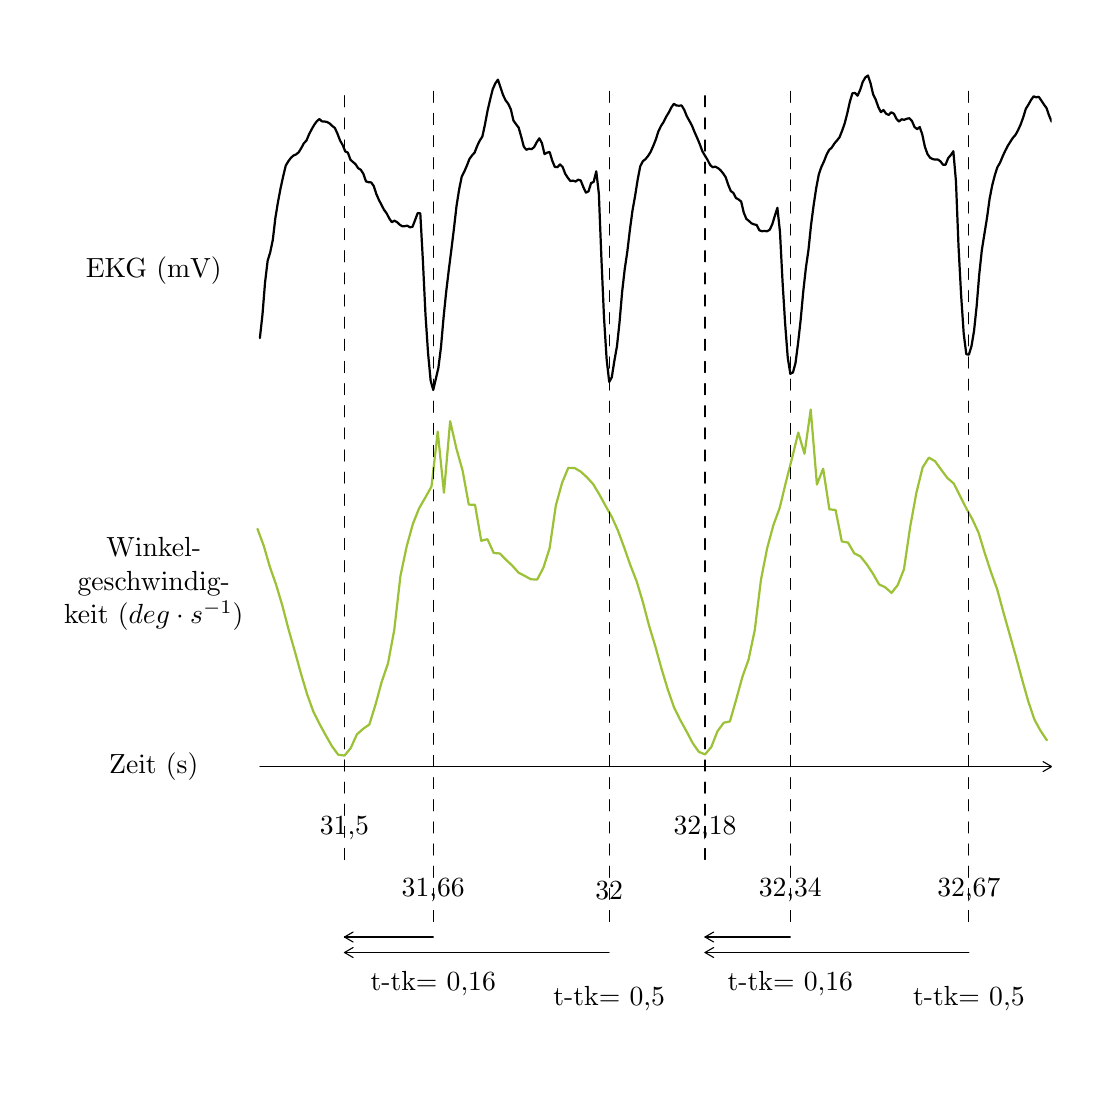
\begin{tikzpicture}[x=1pt,y=1pt]
\definecolor{fillColor}{RGB}{255,255,255}
\path[use as bounding box,fill=fillColor,fill opacity=0.00] (0,0) rectangle (377.25,377.25);
\begin{scope}
\path[clip] (  7.23,  7.23) rectangle (370.02,370.02);
\definecolor{drawColor}{RGB}{0,0,0}

\path[draw=drawColor,line width= 0.8pt,line join=round,line cap=round] ( 83.90,265.09) --
	( 84.84,273.51) --
	( 85.77,285.12) --
	( 86.71,293.00) --
	( 87.64,296.07) --
	( 88.58,300.58) --
	( 89.51,308.54) --
	( 90.45,314.26) --
	( 91.38,319.20) --
	( 92.32,323.51) --
	( 93.25,327.38) --
	( 94.19,328.97) --
	( 95.12,330.21) --
	( 96.06,331.06) --
	( 96.99,331.45) --
	( 97.93,332.22) --
	( 98.86,333.72) --
	( 99.80,335.48) --
	(100.73,336.45) --
	(101.67,338.69) --
	(102.60,340.51) --
	(103.54,342.12) --
	(104.47,343.43) --
	(105.41,344.22) --
	(106.34,343.39) --
	(107.28,343.33) --
	(108.21,343.16) --
	(109.15,342.60) --
	(110.08,341.72) --
	(111.02,341.00) --
	(111.95,338.91) --
	(112.89,336.46) --
	(113.82,334.84) --
	(114.76,332.52) --
	(115.69,332.10) --
	(116.63,329.52) --
	(117.56,328.70) --
	(118.50,327.88) --
	(119.43,326.47) --
	(120.37,325.90) --
	(121.30,324.43) --
	(122.24,321.72) --
	(123.17,321.39) --
	(124.11,321.34) --
	(125.04,320.05) --
	(125.98,317.15) --
	(126.91,315.02) --
	(127.85,313.22) --
	(128.78,311.42) --
	(129.72,310.16) --
	(130.65,308.31) --
	(131.59,306.97) --
	(132.52,307.50) --
	(133.46,306.99) --
	(134.39,306.10) --
	(135.33,305.48) --
	(136.26,305.53) --
	(137.20,305.68) --
	(138.13,305.12) --
	(139.07,305.29) --
	(140.00,307.76) --
	(140.94,310.26) --
	(141.87,310.20) --
	(142.81,293.04) --
	(143.74,273.71) --
	(144.68,259.62) --
	(145.61,249.73) --
	(146.55,246.33) --
	(147.48,250.33) --
	(148.42,254.38) --
	(149.35,261.84) --
	(150.29,272.62) --
	(151.22,281.74) --
	(152.16,289.61) --
	(153.09,296.95) --
	(154.03,304.63) --
	(154.96,312.80) --
	(155.90,318.76) --
	(156.83,323.39) --
	(157.77,325.24) --
	(158.70,327.38) --
	(159.64,329.81) --
	(160.57,331.08) --
	(161.51,332.12) --
	(162.44,334.54) --
	(163.38,336.49) --
	(164.31,337.92) --
	(165.25,342.32) --
	(166.18,347.25) --
	(167.12,351.31) --
	(168.05,355.01) --
	(168.99,357.15) --
	(169.92,358.46) --
	(170.86,355.69) --
	(171.79,352.87) --
	(172.73,350.95) --
	(173.66,349.73) --
	(174.60,347.71) --
	(175.53,343.69) --
	(176.47,342.37) --
	(177.40,341.15) --
	(178.34,337.86) --
	(179.27,334.25) --
	(180.21,333.13) --
	(181.14,333.51) --
	(182.08,333.34) --
	(183.01,334.09) --
	(183.95,335.85) --
	(184.88,337.26) --
	(185.82,335.56) --
	(186.75,331.57) --
	(187.69,332.08) --
	(188.62,332.31) --
	(189.56,329.17) --
	(190.49,326.91) --
	(191.43,326.84) --
	(192.36,327.84) --
	(193.30,326.93) --
	(194.23,324.48) --
	(195.17,323.02) --
	(196.11,321.82) --
	(197.04,321.99) --
	(197.98,321.64) --
	(198.91,322.31) --
	(199.85,322.03) --
	(200.78,319.66) --
	(201.72,317.63) --
	(202.65,318.09) --
	(203.59,321.10) --
	(204.52,321.51) --
	(205.46,325.35) --
	(206.39,317.32) --
	(207.33,293.61) --
	(208.26,272.41) --
	(209.20,257.54) --
	(210.13,249.24) --
	(211.07,250.93) --
	(212.00,256.88) --
	(212.94,262.14) --
	(213.87,270.84) --
	(214.81,281.81) --
	(215.74,289.97) --
	(216.68,296.33) --
	(217.61,304.20) --
	(218.55,311.18) --
	(219.48,316.39) --
	(220.42,322.33) --
	(221.35,327.17) --
	(222.29,329.00) --
	(223.22,329.71) --
	(224.16,330.85) --
	(225.09,332.34) --
	(226.03,334.46) --
	(226.96,336.80) --
	(227.90,339.77) --
	(228.83,341.69) --
	(229.77,343.14) --
	(230.70,345.03) --
	(231.64,346.56) --
	(232.57,348.40) --
	(233.51,349.74) --
	(234.44,349.10) --
	(235.38,349.06) --
	(236.31,349.12) --
	(237.25,347.56) --
	(238.18,345.25) --
	(239.12,343.56) --
	(240.05,341.82) --
	(240.99,339.49) --
	(241.92,337.40) --
	(242.86,335.16) --
	(243.79,332.61) --
	(244.73,331.00) --
	(245.66,329.50) --
	(246.60,327.64) --
	(247.53,326.82) --
	(248.47,327.03) --
	(249.40,326.54) --
	(250.34,325.76) --
	(251.27,324.63) --
	(252.21,323.22) --
	(253.14,320.47) --
	(254.08,318.20) --
	(255.01,317.53) --
	(255.95,315.69) --
	(256.88,315.18) --
	(257.82,314.42) --
	(258.75,310.43) --
	(259.69,308.16) --
	(260.62,307.41) --
	(261.56,306.54) --
	(262.49,306.16) --
	(263.43,305.96) --
	(264.36,304.03) --
	(265.30,303.70) --
	(266.23,303.78) --
	(267.17,303.68) --
	(268.10,304.18) --
	(269.04,306.14) --
	(269.97,309.22) --
	(270.91,312.15) --
	(271.84,303.45) --
	(272.78,285.28) --
	(273.71,270.26) --
	(274.65,258.00) --
	(275.58,252.16) --
	(276.52,252.64) --
	(277.45,256.03) --
	(278.39,263.31) --
	(279.32,271.70) --
	(280.26,281.95) --
	(281.19,290.34) --
	(282.13,296.87) --
	(283.06,305.89) --
	(284.00,313.04) --
	(284.93,319.25) --
	(285.87,324.21) --
	(286.80,326.93) --
	(287.74,328.92) --
	(288.67,331.33) --
	(289.61,333.08) --
	(290.54,333.88) --
	(291.48,335.35) --
	(292.41,336.46) --
	(293.35,337.63) --
	(294.28,339.96) --
	(295.22,342.64) --
	(296.15,346.26) --
	(297.09,350.45) --
	(298.02,353.55) --
	(298.96,353.65) --
	(299.89,352.66) --
	(300.83,354.80) --
	(301.76,357.68) --
	(302.70,359.28) --
	(303.63,359.97) --
	(304.57,357.17) --
	(305.50,353.16) --
	(306.44,351.23) --
	(307.37,348.59) --
	(308.31,346.72) --
	(309.24,347.49) --
	(310.18,346.17) --
	(311.11,345.71) --
	(312.05,346.67) --
	(312.98,346.21) --
	(313.92,344.31) --
	(314.86,343.32) --
	(315.79,344.15) --
	(316.73,343.95) --
	(317.66,344.34) --
	(318.60,344.53) --
	(319.53,343.52) --
	(320.47,341.34) --
	(321.40,340.58) --
	(322.34,341.34) --
	(323.27,338.61) --
	(324.21,334.19) --
	(325.14,331.59) --
	(326.08,330.26) --
	(327.01,329.76) --
	(327.95,329.57) --
	(328.88,329.61) --
	(329.82,328.96) --
	(330.75,327.73) --
	(331.69,327.75) --
	(332.62,330.12) --
	(333.56,331.20) --
	(334.49,332.60) --
	(335.43,321.77) --
	(336.36,298.17) --
	(337.30,280.59) --
	(338.23,266.71) --
	(339.17,259.26) --
	(340.10,259.08) --
	(341.04,262.16) --
	(341.97,267.69) --
	(342.91,276.61) --
	(343.84,288.02) --
	(344.78,296.86) --
	(345.71,302.68) --
	(346.65,308.52) --
	(347.58,315.36) --
	(348.52,320.22) --
	(349.45,323.83) --
	(350.39,326.81) --
	(351.32,328.36) --
	(352.26,330.62) --
	(353.19,332.67) --
	(354.13,334.50) --
	(355.06,335.99) --
	(356.00,337.43) --
	(356.93,338.48) --
	(357.87,340.20) --
	(358.80,342.25) --
	(359.74,344.84) --
	(360.67,347.91) --
	(361.61,349.43) --
	(362.54,351.07) --
	(363.48,352.44) --
	(364.41,352.09) --
	(365.35,352.26) --
	(366.28,350.93) --
	(367.22,349.48) --
	(368.15,348.21) --
	(369.09,345.47) --
	(370.02,343.24);
\end{scope}
\begin{scope}
\path[clip] (  7.23,  7.23) rectangle (370.02,370.02);
\definecolor{drawColor}{RGB}{155,193,54}

\path[draw=drawColor,line width= 0.8pt,line join=round,line cap=round] ( 83.03,196.16) --
	( 85.27,190.13) --
	( 87.52,182.39) --
	( 89.77,175.96) --
	( 92.01,168.47) --
	( 94.26,159.84) --
	( 96.51,151.98) --
	( 98.75,143.84) --
	(101.00,136.30) --
	(103.24,130.07) --
	(105.49,125.59) --
	(107.74,121.48) --
	(109.98,117.57) --
	(112.23,114.52) --
	(114.48,114.23) --
	(116.72,116.92) --
	(118.97,121.89) --
	(121.21,123.88) --
	(123.46,125.43) --
	(125.71,132.72) --
	(127.95,140.94) --
	(130.20,147.54) --
	(132.45,159.51) --
	(134.69,179.10) --
	(136.94,189.76) --
	(139.18,197.91) --
	(141.43,203.57) --
	(143.68,207.44) --
	(145.92,211.47) --
	(148.17,231.26) --
	(150.42,209.19) --
	(152.66,235.08) --
	(154.91,225.19) --
	(157.15,217.21) --
	(159.40,204.91) --
	(161.65,204.83) --
	(163.89,191.84) --
	(166.14,192.41) --
	(168.39,187.44) --
	(170.63,187.24) --
	(172.88,184.92) --
	(175.13,182.84) --
	(177.37,180.32) --
	(179.62,179.14) --
	(181.86,177.92) --
	(184.11,177.83) --
	(186.36,182.11) --
	(188.60,189.15) --
	(190.85,204.59) --
	(193.10,212.77) --
	(195.34,218.19) --
	(197.59,218.15) --
	(199.83,216.84) --
	(202.08,214.77) --
	(204.33,212.32) --
	(206.57,208.58) --
	(208.82,204.46) --
	(211.07,200.47) --
	(213.31,195.47) --
	(215.56,189.36) --
	(217.80,182.96) --
	(220.05,177.18) --
	(222.30,169.69) --
	(224.54,161.14) --
	(226.79,153.73) --
	(229.04,145.59) --
	(231.28,138.18) --
	(233.53,131.70) --
	(235.77,127.14) --
	(238.02,123.07) --
	(240.27,118.79) --
	(242.51,115.58) --
	(244.76,114.64) --
	(247.01,117.29) --
	(249.25,122.99) --
	(251.50,126.08) --
	(253.75,126.57) --
	(255.99,134.35) --
	(258.24,142.61) --
	(260.48,148.88) --
	(262.73,159.55) --
	(264.98,177.83) --
	(267.22,189.19) --
	(269.47,197.54) --
	(271.72,203.65) --
	(273.96,212.93) --
	(276.21,221.73) --
	(278.45,230.93) --
	(280.70,223.28) --
	(282.95,239.28) --
	(285.19,212.16) --
	(287.44,217.90) --
	(289.69,203.20) --
	(291.93,202.96) --
	(294.18,191.60) --
	(296.42,191.19) --
	(298.67,187.32) --
	(300.92,186.18) --
	(303.16,183.37) --
	(305.41,179.99) --
	(307.66,176.08) --
	(309.90,175.02) --
	(312.15,172.99) --
	(314.39,175.84) --
	(316.64,181.54) --
	(318.89,196.89) --
	(321.13,209.19) --
	(323.38,218.31) --
	(325.63,221.89) --
	(327.87,220.59) --
	(330.12,217.49) --
	(332.37,214.48) --
	(334.61,212.57) --
	(336.86,208.13) --
	(339.10,203.69) --
	(341.35,199.62) --
	(343.60,194.77) --
	(345.84,187.36) --
	(348.09,180.52) --
	(350.34,174.25) --
	(352.58,165.99) --
	(354.83,158.05) --
	(357.07,150.11) --
	(359.32,141.76) --
	(361.57,133.78) --
	(363.81,127.18) --
	(366.06,123.07) --
	(368.31,119.73);
\definecolor{drawColor}{RGB}{0,0,0}

\path[draw=drawColor,line width= 0.4pt,dash pattern=on 4pt off 4pt ,line join=round,line cap=round] (114.48, 76.65) -- (114.48,356.59);

\path[draw=drawColor,line width= 0.4pt,dash pattern=on 4pt off 4pt ,line join=round,line cap=round] (244.76, 76.65) -- (244.76,356.59);

\path[draw=drawColor,line width= 0.4pt,dash pattern=on 4pt off 4pt ,line join=round,line cap=round] (146.55, 54.26) -- (146.55,356.59);

\path[draw=drawColor,line width= 0.4pt,dash pattern=on 4pt off 4pt ,line join=round,line cap=round] (210.13, 54.26) -- (210.13,356.59);

\path[draw=drawColor,line width= 0.4pt,dash pattern=on 4pt off 4pt ,line join=round,line cap=round] (275.58, 54.26) -- (275.58,356.59);

\path[draw=drawColor,line width= 0.4pt,dash pattern=on 4pt off 4pt ,line join=round,line cap=round] (340.10, 54.26) -- (340.10,356.59);

\path[draw=drawColor,line width= 0.4pt,line join=round,line cap=round] ( 83.90,110.24) -- (370.02,110.24);

\path[draw=drawColor,line width= 0.4pt,line join=round,line cap=round] (366.89,108.44) --
	(370.02,110.24) --
	(366.89,112.05);

\node[text=drawColor,anchor=base,inner sep=0pt, outer sep=0pt, scale=  1.00] at (114.48, 85.61) {31,5};

\node[text=drawColor,anchor=base,inner sep=0pt, outer sep=0pt, scale=  1.00] at (244.76, 85.61) {32,18};

\node[text=drawColor,anchor=base,inner sep=0pt, outer sep=0pt, scale=  1.00] at (146.55, 63.22) {31,66};

\node[text=drawColor,anchor=base,inner sep=0pt, outer sep=0pt, scale=  1.00] at (210.13, 62.25) {32};

\node[text=drawColor,anchor=base,inner sep=0pt, outer sep=0pt, scale=  1.00] at (275.58, 63.22) {32,34};

\node[text=drawColor,anchor=base,inner sep=0pt, outer sep=0pt, scale=  1.00] at (340.10, 63.22) {32,67};

\node[text=drawColor,anchor=base,inner sep=0pt, outer sep=0pt, scale=  1.00] at ( 45.56,286.90) {EKG (mV)};

\node[text=drawColor,anchor=base,inner sep=0pt, outer sep=0pt, scale=  1.00] at ( 45.56,185.98) {Winkel-};

\node[text=drawColor,anchor=base,inner sep=0pt, outer sep=0pt, scale=  1.00] at ( 45.56,173.98) {geschwindig-};

\node[text=drawColor,anchor=base,inner sep=0pt, outer sep=0pt, scale=  1.00] at ( 45.56,161.98) {keit ($deg \cdot s^{-1}$)};

\node[text=drawColor,anchor=base,inner sep=0pt, outer sep=0pt, scale=  1.00] at ( 45.56,107.74) {Zeit (s)};

\path[draw=drawColor,line width= 0.4pt,line join=round,line cap=round] (146.55, 48.66) -- (114.48, 48.66);

\path[draw=drawColor,line width= 0.4pt,line join=round,line cap=round] (117.60, 50.46) --
	(114.48, 48.66) --
	(117.60, 46.85);

\path[draw=drawColor,line width= 0.4pt,line join=round,line cap=round] (210.13, 43.06) -- (114.48, 43.06);

\path[draw=drawColor,line width= 0.4pt,line join=round,line cap=round] (117.60, 44.87) --
	(114.48, 43.06) --
	(117.60, 41.25);

\path[draw=drawColor,line width= 0.4pt,line join=round,line cap=round] (275.58, 48.66) -- (244.76, 48.66);

\path[draw=drawColor,line width= 0.4pt,line join=round,line cap=round] (247.89, 50.46) --
	(244.76, 48.66) --
	(247.89, 46.85);

\path[draw=drawColor,line width= 0.4pt,line join=round,line cap=round] (340.10, 43.06) -- (244.76, 43.06);

\path[draw=drawColor,line width= 0.4pt,line join=round,line cap=round] (247.89, 44.87) --
	(244.76, 43.06) --
	(247.89, 41.25);

\node[text=drawColor,anchor=base,inner sep=0pt, outer sep=0pt, scale=  1.00] at (146.55, 29.39) {t-tk= 0,16};

\node[text=drawColor,anchor=base,inner sep=0pt, outer sep=0pt, scale=  1.00] at (210.13, 23.79) {t-tk= 0,5};

\node[text=drawColor,anchor=base,inner sep=0pt, outer sep=0pt, scale=  1.00] at (275.58, 29.39) {t-tk= 0,16};

\node[text=drawColor,anchor=base,inner sep=0pt, outer sep=0pt, scale=  1.00] at (340.10, 23.79) {t-tk= 0,5};
\end{scope}
\end{tikzpicture}
 \caption[Grundlage der Berechnung der kardio-lokomotorischen Phasensynchronisation]{Grundlage der Berechnung der kardio-lokomotorischen Phasensynchronisation} \label{fig:grundlage_klps} 
\end{figure}

Die kardio-lokomotorische Phasensynchronisation interpretieren \citet[][S.~12]{Niizeki2014} als ein konsistentes Auftreten eines Herzschlages in der gleichen relativen Phase aufeinanderfolgender Bewegungsabläufe. Das heißt, z.~B. bei einer hohen kardio-lokomotorischen Phasensynchronisation beim Laufen tritt der Herzschlag in der Regel auf, wenn das Bein einen relativen Weg zurückgelegt hat. Die relative Phase beschreibt die Beziehung zwischen Herzschlag und zurückgelegtem Weg im Bewegungsablauf. Zu ihrer Berechnung benötigen wir die momentanen Phasen der beiden Oszillatoren (Herz und Bewegungsapparat). Es gibt zwei Vorgehen, um die momentanen Phasen zu berechnen: ein ereignis-bezogenes Vorgehen und ein signalanalytisches Vorgehen. In der vorliegenden Arbeit beschränke ich mich auf die Erklärung des ereignisbezogenen Vorgehens, da ich die Zeitpunkte unserer beiden Ereignisse (R-Spitze und \ac{MS}) in den vorherigen Verarbeitungsschritten bestimme. Abbildung~\ref{fig:grundlage_klps} stellt die aufeinanderfolgenden Ereignisse dar.

\newpage

Innerhalb eines Oszillators berechnen wir die momentane Phase mit: 
\begin{equation}
	\phi(t) = 2 \pi \frac{t-t_{k}}{t_{k+1}-t_{k}} + 2 \pi k, 
\end{equation}

wobei $t_{k}$ der Zeit des k-ten Ereignisses entspricht. Die relative Phase für das Auftreten eines Herzschlages bezüglich des Bewegungsablaufs berechnen wir demzufolge mit: 
\begin{equation}
	\Psi(t_{k}) = 1 \frac{\phi_{L}(t_{k}) \bmod 2 \pi}{2 \pi}, 
\end{equation}

wobei $t_{k}$ der Zeit des k-ten Auftretens eines Herzschlags und $\phi_{L}$ der momentanen Phase des Bewegungsablaufs entspricht. Stellen wir $\Psi(t_{k})$ über $t_{k}$ dar, erhalten wir das kardio-lokomotorische Synchrogramm. Mit Hilfe des Synchrogramms bin ich in der Lage nachfolgende Aussagen zu treffen: 
\begin{itemize}
	
	\item Sind beide rhythmischen Oszillatoren unabhängig voneinander, gibt es keine bevorzugte Phase. Die Verteilung von $\Psi(t_{k})$ ist zufällig.
	
	\item Tritt alternativ eine $n:m$ Phasensynchronisation auf, d.~h. $\Psi(t_{k})$ tritt genau zu den gleichen $n$ Werten innerhalb der $m$ Bewegungsablauf auf, beobachten wir $n$ parallele horizontale Linien. 
\end{itemize}

Die visuelle Bestimmung der Synchronität erfolgt über ein R-Programm. Das Programm berechnet zur Quantifizierung der kardio-lokomotorischen Phasensynchronisation den Phasenkohärenz Index \citep{Rosenblum2003} und den normalisierten Shannon Entropie Index \citep{Tass1998, Niizeki2005} und stellt sie dar. Indizes und Phasen sichert das Programm in einer Textdatei im \acs{csv}-Format.

% paragraph r_programme_zur_erkennung (end)
% subsubsection psychophysiopipeline (end)
\subsubsection{Programme zur Analyse von zeitbasierten multimodalen Daten} 

% (fold)
\label{ssub:programme_zur_analyse_von_zeitbasierten_multimodalen_daten}

Im \acs{BMBF}-Projekt probierten wir unterschiedliche Software zur Analyse von zeitbasierten multimodalen Daten wie den Observer XT von Noldus aus. Der Observer ist ein Werkzeug, das die parallele Untersuchung von mehreren Datenströmen in der Zeit und mit Bezug auf den geographischen Raum ermöglicht. Den Bezug zum geographischen Raum stellt der Observer über eine zweite Software namens Tracklab her. Der Observer ermöglicht die Annotation der Daten, um konkrete Zeiträume bzw. Phasen genauer durch Verändern des Zoomfaktors zu betrachten. Leider ist der Import von Daten in den Observer und in Tracklab aufwendig. Für beide Programme braucht man teure Lizenzen und die Nutzbarkeit ist für unseren Verwendungszweck nicht befriedigend.

Ein freies Programm namens ChronoViz \citep{Fouse2010, Fouse2011}, welches die Visualisierung von mehreren Datenströmen in Bezug auf einen geographischen Raum ermöglicht, war nicht in der Lage die Menge an Daten zu verarbeiten. Daraus folgt, dass ein benutzerfreundliches Werkzeug, das eine prozessorientierte Untersuchung mit Bezug auf einen geographischen Raum im Bereich der Mensch-Computer-Interaktion fehlt.

Als Konsequenz nutzte ich zur Visualisierung der Datenströme R und zur Visualisierung der geographischen Daten Google Earth, auch wenn ich das Zoomen in die Daten und die Synchronisation der Zeit zwischen Datenpunkt und geographischer Position per Hand vornehmen musste.

% subsubsection programme_zur_analyse_von_zeitbasierten_multimodalen_daten (end)
% subsection apparat (end)
\subsection{Operationalisierung und gewonnene Daten} 

% (fold)
\label{sub:operationalisierung_und_gewonnene_daten_5_1}

Auf der Grundlage der sechs Läufe erhielt ich 24 Selbstauskünfte durch die Befragung mit der \ac{FKS}. Die \ac{FKS} besitzt nach \citet{Rheinberg2003} eine hohe Güte. Nichtsdestotrotz überprüfte ich die gewonnenen Daten nochmals auf ihre Eignung. Ich garantiere damit, dass die aus der Skala ermittelten Messwerte, die zu beschreibenden Faktoren mit hoher Reliabilität wiedergeben. Gleichzeitig prüfe ich, ob ich die \ac{FKS} im vorliegenden Einzelfall einer laufenden Person erfolgreich eingesetzt habe.

Zur Verifizierung betrachtete ich die 24 Selbstauskünfte und bestimmte den Mittelwert und die Standardabweichung jedes Items des Generalfaktors und der beiden Faktoren der \ac{FKS}. Ebenso berechnete ich für jeden Faktor und dessen Items die Item-Faktor-Korrelation. Die Item-Faktor-Korrelation dient häufig als Testgröße der Trennschärfe. Je höher und gleichmäßiger die Trennschärfe ist, desto höher ist die Konsistenz zwischen den Items und desto besser die verwendete Skala. Als Daumenregel gilt, eine Trennschärfe von größer als 0,5 ist passend. Solange die Items nur geringfügig unter 0,5 liegen, sieht man sie als vertretbar an. Wichtig ist in jedem Fall, dass keine der Trennschärfen signifikant von allen übrigen abweicht und dass die Trennschärfen niemals negativ sind \citep[][S.~219f.]{Bortz2006}.

Neben der Trennschärfe der einzelnen Items bestimmte ich für die Faktoren der \ac{FKS} die Maßzahl Cronbachs~$\alpha$, um festzustellen, inwieweit ich die Faktoren zur Messung der einzelnen latenten Wirkungsdimensionen heranziehen kann. Das Cronbachs~$\alpha$ ist eine in den Wirtschafts- und Sozialwissenschaften häufig verwendetes Reliabilitätskriterium in der Testkonstruktion und -evaluation. Vernünftige Werte für das Cronbachs~$\alpha$ sind größer 0,7 \citep[][S.~189f.]{Bortz2006}.

Die Reliabilität des Generalfaktors und der Absorbiertheit weisen mit 0,81 und 0,77 auf eine gute Eignung hin, die Reliabilität des glatten Verlaufs ist mit 0,68 akzeptabel. Die Trennschärfen sind bis auf die Items »Mein Kopf ist völlig klar.« und »Ich weiß bei jedem Schritt, was ich zu tun habe.« für den Generalfaktor, bei denen die Trennschärfe unter 0,4 liegt, akzeptabel (Tabellen~\ref{tab:generalfaktor_1}, \ref{tab:glatter_verlauf_1} und \ref{tab:absorbiertheit_1}). In der Untersuchung hatte das Ergebnis für die Items keine Konsequenzen, da es sich bei \ac{FKS} um eine wissenschaftlich eingehend untersuchte Skala handelt und da ich mögliche inhaltliche Verfälschungen durch weglassen von Items vermeiden wollte.

Zu jedem Befragungszeitpunkt gehören ca. 15 Minuten an \ac{EKG}-Daten und kinematischen Daten, die der \ac{PPC} vor jeder Befragung aufzeichnete. Es sind ca. 15 Minuten, da der Signalgeber nach 15 Minuten die Untersuchungsperson aufforderte, eine Selbstauskunft abzugeben. Das gewährleistete nicht in allen Fällen das Stehenbleiben und das Ausfüllen. Aus diesem Grund verwendete ich die Daten bis zum letzten erkannten Laufschritt vor der Fertigstellung des Fragebogens. Den letzten Laufschritt identifizierte ich im Nachhinein. 

Zur R-Spitzen-Erkennung nutzte ich die Ableitung III, da sie die größten R-Spitzen aufwies. Die R-Spitzen identifiziert Kubios \ac{HRV} in aller Regel automatisch (abhängig von der Signalgüte), trotzdem ist eine manuelle Nachbearbeitung notwendig. Nicht erkannte R-Spitzen fügte ich hinzu und zu viel erkannte R-Spitzen entfernte ich. 

Zur Berechnung des Bewegungsaufwands (Abschnitt~\ref{ssub:der_bewegungsfluss}) für jeden Bewegungsablauf (Doppelschritt) filterte das R-Programm die gemessene Beschleunigung entlang des koronaren Schnittes (von rechts nach links, X-Achse), entlang des sagittalen Schnittes (von unten nach oben, Y-Achse) und entlang des axialen Schnittes (von hinten nach vorne, Z-Achse) mit den optimalen Grenzfrequenzen von 1,5~Hz, 4,0~Hz und 5,5~Hz.

Die kardio-lokomotorische Phasensynchronisation (Abschnitt~\ref{ssub:die_kardio_lokomotorische_phasensynchronisation}) quantifizierte ich durch den normalisierten Shannon Entropie Index. Zur Berechnung der Shannon Entropie nutzte ich ein 15 Sekunden Fenster der relativen Phase und verschob dieses jeweils um eine Sekunde, um aufeinanderfolgende Werte zu erhalten. Zur Berechnung der Shannon Entropie teilte ich den Messbereich der relativen Phase (0 bis 1) in eine optimale Anzahl von Abschnitten mit $N = exp(0{,}626 + 0{,}4 \cdot ln(M-1))$, wobei $M$ die Anzahl der Werte der relativen Phase im Zeitfenster darstellt \citep[][S.~20]{Rosenblum2003}.

Um Zusammenhänge zwischen den expliziten Flow-Merkmalen der \ac{FKS} und impliziten Merkmalen zu untersuchen (Anschnitt~\ref{sec:herangehensweise}, Schritt~2), berechnete ich akkumulierte implizite Merkmale der Kurzzeit-\ac{HRV} (mittlere \ac{HR} und \acs{RMSSD}), des Bewegungsaufwands (mittlerer Bewegungsaufwand und mittlere Doppelschrittfrequenz) und der kardio-lokomotorische Phasensynchronisation (mittlerer normalisierter Shannon Entropie Index). Als Datengrundlage nutzte ich die fünf Minuten an Daten direkt vor der Befragung mit der \ac{FKS}, da die \ac{FKS} den gegenwärtigen Flow-Zustand mit Items (Aussagen) wie »Ich fühle mich optimal beansprucht.« abfragt. Dabei halte ich die Länge von fünf Minuten für einen guten Kompromiss, da ich damit die empfohlene Länge für die Berechnungen der Kurzzeit-\ac{HRV} \citep[][S.~360]{TaskForce1996} einhalte und genügend Anlaufzeit nach dem Start des Laufes und nach jeder Unterbrechung durch die Befragung mit der \ac{FKS} bleibt (Kapitel~\ref{cha:flow_erleben_beim_gehen_und_laufen_messen_anforderungen}). Zusätzlich musste ich bei der Datenlänge von fünf Minuten keine \ac{EKG}-Messung aufgrund von vielen Artefakten aus der Datenbasis entfernen, was bei längeren Zeitspannen der Fall gewesen wäre und was zu einer ungleichen Anzahl von expliziten und impliziten Merkmalen geführt hätte.

% subsection operationalisierung_und_gewonnene_daten (end)
\subsection{Ergebnisse} 

% (fold)
\label{sub:ergebnisse_5_1}

\subsubsection{Beobachtungen} 

% (fold)
\label{ssub:beobachtungen_5_1} 
\begin{figure}
	[!htb] % Created by tikzDevice version 0.10.1 on 2016-09-06 19:52:25
% !TEX encoding = UTF-8 Unicode
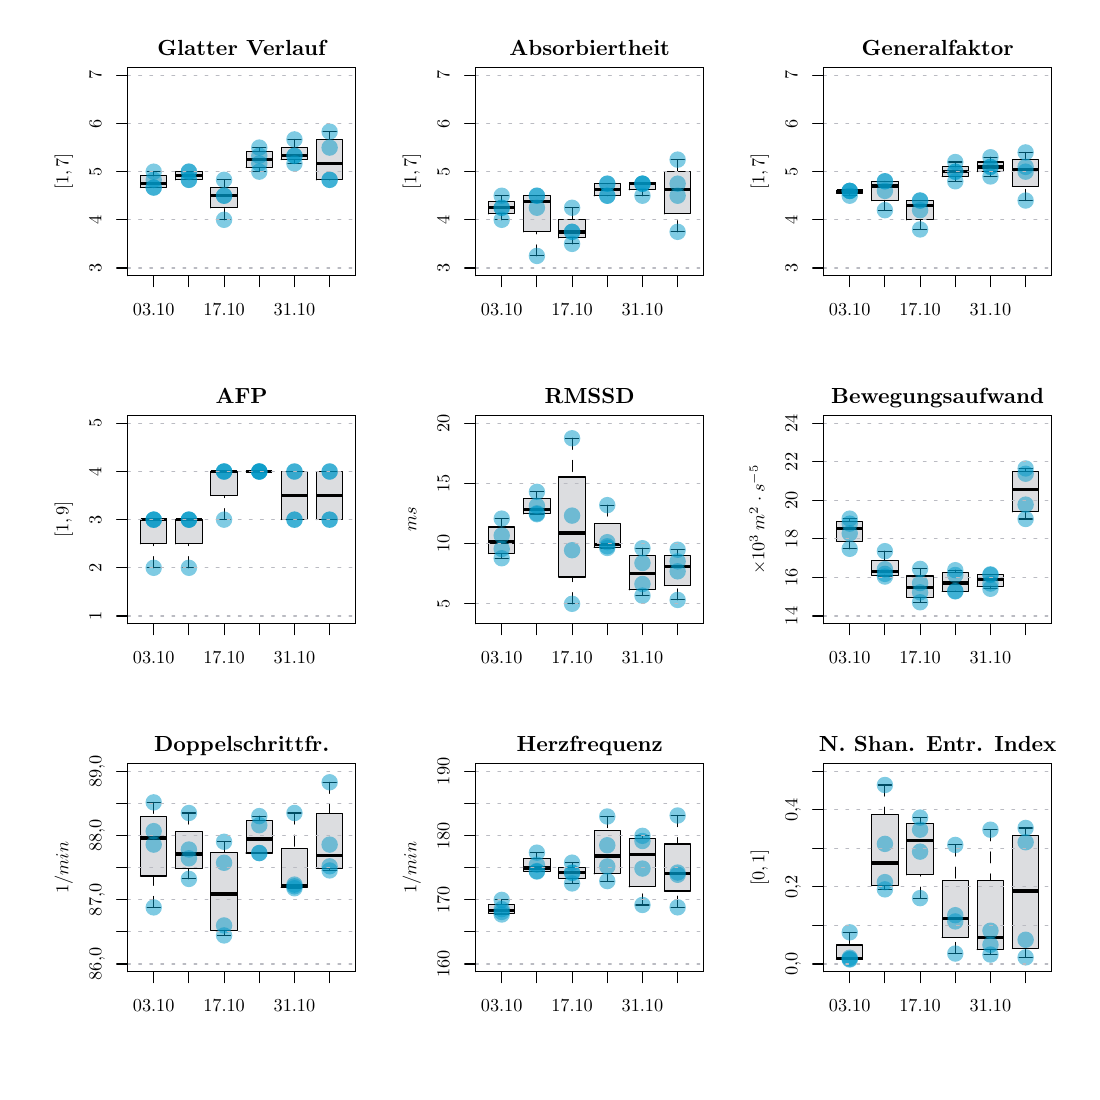
\begin{tikzpicture}[x=1pt,y=1pt]
\definecolor{fillColor}{RGB}{255,255,255}
\path[use as bounding box,fill=fillColor,fill opacity=0.00] (0,0) rectangle (377.25,377.25);
\begin{scope}
\path[clip] ( 36.13,287.63) rectangle (118.52,362.80);
\definecolor{fillColor}{RGB}{186,187,194}

\path[fill=fillColor,fill opacity=0.50] ( 40.78,319.47) --
	( 50.31,319.47) --
	( 50.31,323.74) --
	( 40.78,323.74) --
	cycle;
\definecolor{drawColor}{RGB}{0,0,0}

\path[draw=drawColor,line width= 1.2pt,line join=round] ( 40.78,320.87) -- ( 50.31,320.87);

\path[draw=drawColor,line width= 0.4pt,dash pattern=on 4pt off 4pt ,line join=round,line cap=round] ( 45.54,319.47) -- ( 45.54,319.47);

\path[draw=drawColor,line width= 0.4pt,dash pattern=on 4pt off 4pt ,line join=round,line cap=round] ( 45.54,325.21) -- ( 45.54,323.74);

\path[draw=drawColor,line width= 0.4pt,line join=round,line cap=round] ( 43.16,319.47) -- ( 47.93,319.47);

\path[draw=drawColor,line width= 0.4pt,line join=round,line cap=round] ( 43.16,325.21) -- ( 47.93,325.21);

\path[draw=drawColor,line width= 0.4pt,line join=round,line cap=round] ( 40.78,319.47) --
	( 50.31,319.47) --
	( 50.31,323.74) --
	( 40.78,323.74) --
	( 40.78,319.47);

\path[fill=fillColor,fill opacity=0.50] ( 53.49,322.26) --
	( 63.03,322.26) --
	( 63.03,325.21) --
	( 53.49,325.21) --
	cycle;

\path[draw=drawColor,line width= 1.2pt,line join=round] ( 53.49,323.74) -- ( 63.03,323.74);

\path[draw=drawColor,line width= 0.4pt,dash pattern=on 4pt off 4pt ,line join=round,line cap=round] ( 58.26,322.26) -- ( 58.26,322.26);

\path[draw=drawColor,line width= 0.4pt,dash pattern=on 4pt off 4pt ,line join=round,line cap=round] ( 58.26,325.21) -- ( 58.26,325.21);

\path[draw=drawColor,line width= 0.4pt,line join=round,line cap=round] ( 55.87,322.26) -- ( 60.64,322.26);

\path[draw=drawColor,line width= 0.4pt,line join=round,line cap=round] ( 55.87,325.21) -- ( 60.64,325.21);

\path[draw=drawColor,line width= 0.4pt,line join=round,line cap=round] ( 53.49,322.26) --
	( 63.03,322.26) --
	( 63.03,325.21) --
	( 53.49,325.21) --
	( 53.49,322.26);

\path[fill=fillColor,fill opacity=0.50] ( 66.20,312.17) --
	( 75.74,312.17) --
	( 75.74,319.39) --
	( 66.20,319.39) --
	cycle;

\path[draw=drawColor,line width= 1.2pt,line join=round] ( 66.20,316.52) -- ( 75.74,316.52);

\path[draw=drawColor,line width= 0.4pt,dash pattern=on 4pt off 4pt ,line join=round,line cap=round] ( 70.97,307.82) -- ( 70.97,312.17);

\path[draw=drawColor,line width= 0.4pt,dash pattern=on 4pt off 4pt ,line join=round,line cap=round] ( 70.97,322.26) -- ( 70.97,319.39);

\path[draw=drawColor,line width= 0.4pt,line join=round,line cap=round] ( 68.59,307.82) -- ( 73.36,307.82);

\path[draw=drawColor,line width= 0.4pt,line join=round,line cap=round] ( 68.59,322.26) -- ( 73.36,322.26);

\path[draw=drawColor,line width= 0.4pt,line join=round,line cap=round] ( 66.20,312.17) --
	( 75.74,312.17) --
	( 75.74,319.39) --
	( 66.20,319.39) --
	( 66.20,312.17);

\path[fill=fillColor,fill opacity=0.50] ( 78.92,326.69) --
	( 88.45,326.69) --
	( 88.45,332.44) --
	( 78.92,332.44) --
	cycle;

\path[draw=drawColor,line width= 1.2pt,line join=round] ( 78.92,329.56) -- ( 88.45,329.56);

\path[draw=drawColor,line width= 0.4pt,dash pattern=on 4pt off 4pt ,line join=round,line cap=round] ( 83.69,325.21) -- ( 83.69,326.69);

\path[draw=drawColor,line width= 0.4pt,dash pattern=on 4pt off 4pt ,line join=round,line cap=round] ( 83.69,333.91) -- ( 83.69,332.44);

\path[draw=drawColor,line width= 0.4pt,line join=round,line cap=round] ( 81.30,325.21) -- ( 86.07,325.21);

\path[draw=drawColor,line width= 0.4pt,line join=round,line cap=round] ( 81.30,333.91) -- ( 86.07,333.91);

\path[draw=drawColor,line width= 0.4pt,line join=round,line cap=round] ( 78.92,326.69) --
	( 88.45,326.69) --
	( 88.45,332.44) --
	( 78.92,332.44) --
	( 78.92,326.69);

\path[fill=fillColor,fill opacity=0.50] ( 91.63,329.56) --
	(101.17,329.56) --
	(101.17,333.91) --
	( 91.63,333.91) --
	cycle;

\path[draw=drawColor,line width= 1.2pt,line join=round] ( 91.63,330.96) -- (101.17,330.96);

\path[draw=drawColor,line width= 0.4pt,dash pattern=on 4pt off 4pt ,line join=round,line cap=round] ( 96.40,328.17) -- ( 96.40,329.56);

\path[draw=drawColor,line width= 0.4pt,dash pattern=on 4pt off 4pt ,line join=round,line cap=round] ( 96.40,336.87) -- ( 96.40,333.91);

\path[draw=drawColor,line width= 0.4pt,line join=round,line cap=round] ( 94.02,328.17) -- ( 98.78,328.17);

\path[draw=drawColor,line width= 0.4pt,line join=round,line cap=round] ( 94.02,336.87) -- ( 98.78,336.87);

\path[draw=drawColor,line width= 0.4pt,line join=round,line cap=round] ( 91.63,329.56) --
	(101.17,329.56) --
	(101.17,333.91) --
	( 91.63,333.91) --
	( 91.63,329.56);

\path[fill=fillColor,fill opacity=0.50] (104.35,322.26) --
	(113.88,322.26) --
	(113.88,336.78) --
	(104.35,336.78) --
	cycle;

\path[draw=drawColor,line width= 1.2pt,line join=round] (104.35,328.09) -- (113.88,328.09);

\path[draw=drawColor,line width= 0.4pt,dash pattern=on 4pt off 4pt ,line join=round,line cap=round] (109.11,322.26) -- (109.11,322.26);

\path[draw=drawColor,line width= 0.4pt,dash pattern=on 4pt off 4pt ,line join=round,line cap=round] (109.11,339.66) -- (109.11,336.78);

\path[draw=drawColor,line width= 0.4pt,line join=round,line cap=round] (106.73,322.26) -- (111.50,322.26);

\path[draw=drawColor,line width= 0.4pt,line join=round,line cap=round] (106.73,339.66) -- (111.50,339.66);

\path[draw=drawColor,line width= 0.4pt,line join=round,line cap=round] (104.35,322.26) --
	(113.88,322.26) --
	(113.88,336.78) --
	(104.35,336.78) --
	(104.35,322.26);
\end{scope}
\begin{scope}
\path[clip] (  0.00,  0.00) rectangle (377.25,377.25);
\definecolor{drawColor}{RGB}{0,0,0}

\path[draw=drawColor,line width= 0.4pt,line join=round,line cap=round] ( 45.54,287.63) -- (109.11,287.63);

\path[draw=drawColor,line width= 0.4pt,line join=round,line cap=round] ( 45.54,287.63) -- ( 45.54,283.67);

\path[draw=drawColor,line width= 0.4pt,line join=round,line cap=round] ( 58.26,287.63) -- ( 58.26,283.67);

\path[draw=drawColor,line width= 0.4pt,line join=round,line cap=round] ( 70.97,287.63) -- ( 70.97,283.67);

\path[draw=drawColor,line width= 0.4pt,line join=round,line cap=round] ( 83.69,287.63) -- ( 83.69,283.67);

\path[draw=drawColor,line width= 0.4pt,line join=round,line cap=round] ( 96.40,287.63) -- ( 96.40,283.67);

\path[draw=drawColor,line width= 0.4pt,line join=round,line cap=round] (109.11,287.63) -- (109.11,283.67);

\node[text=drawColor,anchor=base,inner sep=0pt, outer sep=0pt, scale=  0.66] at ( 45.54,273.38) {03.10};

\node[text=drawColor,anchor=base,inner sep=0pt, outer sep=0pt, scale=  0.66] at ( 70.97,273.38) {17.10};

\node[text=drawColor,anchor=base,inner sep=0pt, outer sep=0pt, scale=  0.66] at ( 96.40,273.38) {31.10};

\path[draw=drawColor,line width= 0.4pt,line join=round,line cap=round] ( 36.13,290.42) -- ( 36.13,360.01);

\path[draw=drawColor,line width= 0.4pt,line join=round,line cap=round] ( 36.13,290.42) -- ( 32.17,290.42);

\path[draw=drawColor,line width= 0.4pt,line join=round,line cap=round] ( 36.13,307.82) -- ( 32.17,307.82);

\path[draw=drawColor,line width= 0.4pt,line join=round,line cap=round] ( 36.13,325.21) -- ( 32.17,325.21);

\path[draw=drawColor,line width= 0.4pt,line join=round,line cap=round] ( 36.13,342.61) -- ( 32.17,342.61);

\path[draw=drawColor,line width= 0.4pt,line join=round,line cap=round] ( 36.13,360.01) -- ( 32.17,360.01);

\node[text=drawColor,rotate= 90.00,anchor=base,inner sep=0pt, outer sep=0pt, scale=  0.66] at ( 26.63,290.42) {3};

\node[text=drawColor,rotate= 90.00,anchor=base,inner sep=0pt, outer sep=0pt, scale=  0.66] at ( 26.63,307.82) {4};

\node[text=drawColor,rotate= 90.00,anchor=base,inner sep=0pt, outer sep=0pt, scale=  0.66] at ( 26.63,325.21) {5};

\node[text=drawColor,rotate= 90.00,anchor=base,inner sep=0pt, outer sep=0pt, scale=  0.66] at ( 26.63,342.61) {6};

\node[text=drawColor,rotate= 90.00,anchor=base,inner sep=0pt, outer sep=0pt, scale=  0.66] at ( 26.63,360.01) {7};
\end{scope}
\begin{scope}
\path[clip] (  0.00,251.50) rectangle (125.75,377.25);
\definecolor{drawColor}{RGB}{0,0,0}

\node[text=drawColor,anchor=base,inner sep=0pt, outer sep=0pt, scale=  0.79] at ( 77.33,367.29) {\bfseries Glatter Verlauf};

\node[text=drawColor,rotate= 90.00,anchor=base,inner sep=0pt, outer sep=0pt, scale=  0.66] at ( 14.75,325.21) {$[1, 7]$};
\end{scope}
\begin{scope}
\path[clip] (  0.00,  0.00) rectangle (377.25,377.25);
\definecolor{drawColor}{RGB}{0,0,0}

\path[draw=drawColor,line width= 0.4pt,line join=round,line cap=round] ( 36.13,287.63) --
	(118.52,287.63) --
	(118.52,362.80) --
	( 36.13,362.80) --
	( 36.13,287.63);
\end{scope}
\begin{scope}
\path[clip] ( 36.13,287.63) rectangle (118.52,362.80);
\definecolor{fillColor}{RGB}{0,152,199}

\path[fill=fillColor,fill opacity=0.50] ( 45.54,325.21) circle (  2.97);

\path[fill=fillColor,fill opacity=0.50] ( 45.54,322.26) circle (  2.97);

\path[fill=fillColor,fill opacity=0.50] ( 45.54,319.47) circle (  2.97);

\path[fill=fillColor,fill opacity=0.50] ( 45.54,319.47) circle (  2.97);

\path[fill=fillColor,fill opacity=0.50] ( 58.26,322.26) circle (  2.97);

\path[fill=fillColor,fill opacity=0.50] ( 58.26,325.21) circle (  2.97);

\path[fill=fillColor,fill opacity=0.50] ( 58.26,325.21) circle (  2.97);

\path[fill=fillColor,fill opacity=0.50] ( 58.26,322.26) circle (  2.97);

\path[fill=fillColor,fill opacity=0.50] ( 70.97,322.26) circle (  2.97);

\path[fill=fillColor,fill opacity=0.50] ( 70.97,316.52) circle (  2.97);

\path[fill=fillColor,fill opacity=0.50] ( 70.97,307.82) circle (  2.97);

\path[fill=fillColor,fill opacity=0.50] ( 70.97,316.52) circle (  2.97);

\path[fill=fillColor,fill opacity=0.50] ( 83.69,330.96) circle (  2.97);

\path[fill=fillColor,fill opacity=0.50] ( 83.69,325.21) circle (  2.97);

\path[fill=fillColor,fill opacity=0.50] ( 83.69,333.91) circle (  2.97);

\path[fill=fillColor,fill opacity=0.50] ( 83.69,328.17) circle (  2.97);

\path[fill=fillColor,fill opacity=0.50] ( 96.40,330.96) circle (  2.97);

\path[fill=fillColor,fill opacity=0.50] ( 96.40,328.17) circle (  2.97);

\path[fill=fillColor,fill opacity=0.50] ( 96.40,330.96) circle (  2.97);

\path[fill=fillColor,fill opacity=0.50] ( 96.40,336.87) circle (  2.97);

\path[fill=fillColor,fill opacity=0.50] (109.11,339.66) circle (  2.97);

\path[fill=fillColor,fill opacity=0.50] (109.11,333.91) circle (  2.97);

\path[fill=fillColor,fill opacity=0.50] (109.11,322.26) circle (  2.97);

\path[fill=fillColor,fill opacity=0.50] (109.11,322.26) circle (  2.97);
\definecolor{drawColor}{RGB}{186,187,194}

\path[draw=drawColor,line width= 0.4pt,dash pattern=on 1pt off 3pt ,line join=round,line cap=round] ( 36.13,290.42) -- (118.52,290.42);

\path[draw=drawColor,line width= 0.4pt,dash pattern=on 1pt off 3pt ,line join=round,line cap=round] ( 36.13,307.82) -- (118.52,307.82);

\path[draw=drawColor,line width= 0.4pt,dash pattern=on 1pt off 3pt ,line join=round,line cap=round] ( 36.13,325.21) -- (118.52,325.21);

\path[draw=drawColor,line width= 0.4pt,dash pattern=on 1pt off 3pt ,line join=round,line cap=round] ( 36.13,342.61) -- (118.52,342.61);

\path[draw=drawColor,line width= 0.4pt,dash pattern=on 1pt off 3pt ,line join=round,line cap=round] ( 36.13,360.01) -- (118.52,360.01);
\end{scope}
\begin{scope}
\path[clip] (  0.00,  0.00) rectangle (377.25,377.25);
\definecolor{drawColor}{RGB}{0,0,0}

\path[draw=drawColor,line width= 0.4pt,line join=round,line cap=round] ( 36.13,287.63) --
	(118.52,287.63) --
	(118.52,362.80) --
	( 36.13,362.80) --
	( 36.13,287.63);
\end{scope}
\begin{scope}
\path[clip] (161.88,287.63) rectangle (244.27,362.80);
\definecolor{fillColor}{RGB}{186,187,194}

\path[fill=fillColor,fill opacity=0.50] (166.53,309.99) --
	(176.06,309.99) --
	(176.06,314.34) --
	(166.53,314.34) --
	cycle;
\definecolor{drawColor}{RGB}{0,0,0}

\path[draw=drawColor,line width= 1.2pt,line join=round] (166.53,312.17) -- (176.06,312.17);

\path[draw=drawColor,line width= 0.4pt,dash pattern=on 4pt off 4pt ,line join=round,line cap=round] (171.29,307.82) -- (171.29,309.99);

\path[draw=drawColor,line width= 0.4pt,dash pattern=on 4pt off 4pt ,line join=round,line cap=round] (171.29,316.52) -- (171.29,314.34);

\path[draw=drawColor,line width= 0.4pt,line join=round,line cap=round] (168.91,307.82) -- (173.68,307.82);

\path[draw=drawColor,line width= 0.4pt,line join=round,line cap=round] (168.91,316.52) -- (173.68,316.52);

\path[draw=drawColor,line width= 0.4pt,line join=round,line cap=round] (166.53,309.99) --
	(176.06,309.99) --
	(176.06,314.34) --
	(166.53,314.34) --
	(166.53,309.99);

\path[fill=fillColor,fill opacity=0.50] (179.24,303.47) --
	(188.78,303.47) --
	(188.78,316.52) --
	(179.24,316.52) --
	cycle;

\path[draw=drawColor,line width= 1.2pt,line join=round] (179.24,314.34) -- (188.78,314.34);

\path[draw=drawColor,line width= 0.4pt,dash pattern=on 4pt off 4pt ,line join=round,line cap=round] (184.01,294.77) -- (184.01,303.47);

\path[draw=drawColor,line width= 0.4pt,dash pattern=on 4pt off 4pt ,line join=round,line cap=round] (184.01,316.52) -- (184.01,316.52);

\path[draw=drawColor,line width= 0.4pt,line join=round,line cap=round] (181.62,294.77) -- (186.39,294.77);

\path[draw=drawColor,line width= 0.4pt,line join=round,line cap=round] (181.62,316.52) -- (186.39,316.52);

\path[draw=drawColor,line width= 0.4pt,line join=round,line cap=round] (179.24,303.47) --
	(188.78,303.47) --
	(188.78,316.52) --
	(179.24,316.52) --
	(179.24,303.47);

\path[fill=fillColor,fill opacity=0.50] (191.95,301.29) --
	(201.49,301.29) --
	(201.49,307.82) --
	(191.95,307.82) --
	cycle;

\path[draw=drawColor,line width= 1.2pt,line join=round] (191.95,303.47) -- (201.49,303.47);

\path[draw=drawColor,line width= 0.4pt,dash pattern=on 4pt off 4pt ,line join=round,line cap=round] (196.72,299.12) -- (196.72,301.29);

\path[draw=drawColor,line width= 0.4pt,dash pattern=on 4pt off 4pt ,line join=round,line cap=round] (196.72,312.17) -- (196.72,307.82);

\path[draw=drawColor,line width= 0.4pt,line join=round,line cap=round] (194.34,299.12) -- (199.11,299.12);

\path[draw=drawColor,line width= 0.4pt,line join=round,line cap=round] (194.34,312.17) -- (199.11,312.17);

\path[draw=drawColor,line width= 0.4pt,line join=round,line cap=round] (191.95,301.29) --
	(201.49,301.29) --
	(201.49,307.82) --
	(191.95,307.82) --
	(191.95,301.29);

\path[fill=fillColor,fill opacity=0.50] (204.67,316.52) --
	(214.20,316.52) --
	(214.20,320.87) --
	(204.67,320.87) --
	cycle;

\path[draw=drawColor,line width= 1.2pt,line join=round] (204.67,318.69) -- (214.20,318.69);

\path[draw=drawColor,line width= 0.4pt,dash pattern=on 4pt off 4pt ,line join=round,line cap=round] (209.44,316.52) -- (209.44,316.52);

\path[draw=drawColor,line width= 0.4pt,dash pattern=on 4pt off 4pt ,line join=round,line cap=round] (209.44,320.87) -- (209.44,320.87);

\path[draw=drawColor,line width= 0.4pt,line join=round,line cap=round] (207.05,316.52) -- (211.82,316.52);

\path[draw=drawColor,line width= 0.4pt,line join=round,line cap=round] (207.05,320.87) -- (211.82,320.87);

\path[draw=drawColor,line width= 0.4pt,line join=round,line cap=round] (204.67,316.52) --
	(214.20,316.52) --
	(214.20,320.87) --
	(204.67,320.87) --
	(204.67,316.52);

\path[fill=fillColor,fill opacity=0.50] (217.38,318.69) --
	(226.92,318.69) --
	(226.92,320.87) --
	(217.38,320.87) --
	cycle;

\path[draw=drawColor,line width= 1.2pt,line join=round] (217.38,320.87) -- (226.92,320.87);

\path[draw=drawColor,line width= 0.4pt,dash pattern=on 4pt off 4pt ,line join=round,line cap=round] (222.15,316.52) -- (222.15,318.69);

\path[draw=drawColor,line width= 0.4pt,dash pattern=on 4pt off 4pt ,line join=round,line cap=round] (222.15,320.87) -- (222.15,320.87);

\path[draw=drawColor,line width= 0.4pt,line join=round,line cap=round] (219.77,316.52) -- (224.53,316.52);

\path[draw=drawColor,line width= 0.4pt,line join=round,line cap=round] (219.77,320.87) -- (224.53,320.87);

\path[draw=drawColor,line width= 0.4pt,line join=round,line cap=round] (217.38,318.69) --
	(226.92,318.69) --
	(226.92,320.87) --
	(217.38,320.87) --
	(217.38,318.69);

\path[fill=fillColor,fill opacity=0.50] (230.10,309.99) --
	(239.63,309.99) --
	(239.63,325.21) --
	(230.10,325.21) --
	cycle;

\path[draw=drawColor,line width= 1.2pt,line join=round] (230.10,318.69) -- (239.63,318.69);

\path[draw=drawColor,line width= 0.4pt,dash pattern=on 4pt off 4pt ,line join=round,line cap=round] (234.86,303.47) -- (234.86,309.99);

\path[draw=drawColor,line width= 0.4pt,dash pattern=on 4pt off 4pt ,line join=round,line cap=round] (234.86,329.56) -- (234.86,325.21);

\path[draw=drawColor,line width= 0.4pt,line join=round,line cap=round] (232.48,303.47) -- (237.25,303.47);

\path[draw=drawColor,line width= 0.4pt,line join=round,line cap=round] (232.48,329.56) -- (237.25,329.56);

\path[draw=drawColor,line width= 0.4pt,line join=round,line cap=round] (230.10,309.99) --
	(239.63,309.99) --
	(239.63,325.21) --
	(230.10,325.21) --
	(230.10,309.99);
\end{scope}
\begin{scope}
\path[clip] (  0.00,  0.00) rectangle (377.25,377.25);
\definecolor{drawColor}{RGB}{0,0,0}

\path[draw=drawColor,line width= 0.4pt,line join=round,line cap=round] (171.29,287.63) -- (234.86,287.63);

\path[draw=drawColor,line width= 0.4pt,line join=round,line cap=round] (171.29,287.63) -- (171.29,283.67);

\path[draw=drawColor,line width= 0.4pt,line join=round,line cap=round] (184.01,287.63) -- (184.01,283.67);

\path[draw=drawColor,line width= 0.4pt,line join=round,line cap=round] (196.72,287.63) -- (196.72,283.67);

\path[draw=drawColor,line width= 0.4pt,line join=round,line cap=round] (209.44,287.63) -- (209.44,283.67);

\path[draw=drawColor,line width= 0.4pt,line join=round,line cap=round] (222.15,287.63) -- (222.15,283.67);

\path[draw=drawColor,line width= 0.4pt,line join=round,line cap=round] (234.86,287.63) -- (234.86,283.67);

\node[text=drawColor,anchor=base,inner sep=0pt, outer sep=0pt, scale=  0.66] at (171.29,273.38) {03.10};

\node[text=drawColor,anchor=base,inner sep=0pt, outer sep=0pt, scale=  0.66] at (196.72,273.38) {17.10};

\node[text=drawColor,anchor=base,inner sep=0pt, outer sep=0pt, scale=  0.66] at (222.15,273.38) {31.10};

\path[draw=drawColor,line width= 0.4pt,line join=round,line cap=round] (161.88,290.42) -- (161.88,360.01);

\path[draw=drawColor,line width= 0.4pt,line join=round,line cap=round] (161.88,290.42) -- (157.92,290.42);

\path[draw=drawColor,line width= 0.4pt,line join=round,line cap=round] (161.88,307.82) -- (157.92,307.82);

\path[draw=drawColor,line width= 0.4pt,line join=round,line cap=round] (161.88,325.21) -- (157.92,325.21);

\path[draw=drawColor,line width= 0.4pt,line join=round,line cap=round] (161.88,342.61) -- (157.92,342.61);

\path[draw=drawColor,line width= 0.4pt,line join=round,line cap=round] (161.88,360.01) -- (157.92,360.01);

\node[text=drawColor,rotate= 90.00,anchor=base,inner sep=0pt, outer sep=0pt, scale=  0.66] at (152.38,290.42) {3};

\node[text=drawColor,rotate= 90.00,anchor=base,inner sep=0pt, outer sep=0pt, scale=  0.66] at (152.38,307.82) {4};

\node[text=drawColor,rotate= 90.00,anchor=base,inner sep=0pt, outer sep=0pt, scale=  0.66] at (152.38,325.21) {5};

\node[text=drawColor,rotate= 90.00,anchor=base,inner sep=0pt, outer sep=0pt, scale=  0.66] at (152.38,342.61) {6};

\node[text=drawColor,rotate= 90.00,anchor=base,inner sep=0pt, outer sep=0pt, scale=  0.66] at (152.38,360.01) {7};
\end{scope}
\begin{scope}
\path[clip] (125.75,251.50) rectangle (251.50,377.25);
\definecolor{drawColor}{RGB}{0,0,0}

\node[text=drawColor,anchor=base,inner sep=0pt, outer sep=0pt, scale=  0.79] at (203.08,367.29) {\bfseries Absorbiertheit};

\node[text=drawColor,rotate= 90.00,anchor=base,inner sep=0pt, outer sep=0pt, scale=  0.66] at (140.50,325.21) {$[1, 7]$};
\end{scope}
\begin{scope}
\path[clip] (  0.00,  0.00) rectangle (377.25,377.25);
\definecolor{drawColor}{RGB}{0,0,0}

\path[draw=drawColor,line width= 0.4pt,line join=round,line cap=round] (161.88,287.63) --
	(244.27,287.63) --
	(244.27,362.80) --
	(161.88,362.80) --
	(161.88,287.63);
\end{scope}
\begin{scope}
\path[clip] (161.88,287.63) rectangle (244.27,362.80);
\definecolor{fillColor}{RGB}{0,152,199}

\path[fill=fillColor,fill opacity=0.50] (171.29,307.82) circle (  2.97);

\path[fill=fillColor,fill opacity=0.50] (171.29,312.17) circle (  2.97);

\path[fill=fillColor,fill opacity=0.50] (171.29,316.52) circle (  2.97);

\path[fill=fillColor,fill opacity=0.50] (171.29,312.17) circle (  2.97);

\path[fill=fillColor,fill opacity=0.50] (184.01,294.77) circle (  2.97);

\path[fill=fillColor,fill opacity=0.50] (184.01,316.52) circle (  2.97);

\path[fill=fillColor,fill opacity=0.50] (184.01,316.52) circle (  2.97);

\path[fill=fillColor,fill opacity=0.50] (184.01,312.17) circle (  2.97);

\path[fill=fillColor,fill opacity=0.50] (196.72,303.47) circle (  2.97);

\path[fill=fillColor,fill opacity=0.50] (196.72,303.47) circle (  2.97);

\path[fill=fillColor,fill opacity=0.50] (196.72,299.12) circle (  2.97);

\path[fill=fillColor,fill opacity=0.50] (196.72,312.17) circle (  2.97);

\path[fill=fillColor,fill opacity=0.50] (209.44,316.52) circle (  2.97);

\path[fill=fillColor,fill opacity=0.50] (209.44,316.52) circle (  2.97);

\path[fill=fillColor,fill opacity=0.50] (209.44,320.87) circle (  2.97);

\path[fill=fillColor,fill opacity=0.50] (209.44,320.87) circle (  2.97);

\path[fill=fillColor,fill opacity=0.50] (222.15,320.87) circle (  2.97);

\path[fill=fillColor,fill opacity=0.50] (222.15,316.52) circle (  2.97);

\path[fill=fillColor,fill opacity=0.50] (222.15,320.87) circle (  2.97);

\path[fill=fillColor,fill opacity=0.50] (222.15,320.87) circle (  2.97);

\path[fill=fillColor,fill opacity=0.50] (234.86,320.87) circle (  2.97);

\path[fill=fillColor,fill opacity=0.50] (234.86,316.52) circle (  2.97);

\path[fill=fillColor,fill opacity=0.50] (234.86,329.56) circle (  2.97);

\path[fill=fillColor,fill opacity=0.50] (234.86,303.47) circle (  2.97);
\definecolor{drawColor}{RGB}{186,187,194}

\path[draw=drawColor,line width= 0.4pt,dash pattern=on 1pt off 3pt ,line join=round,line cap=round] (161.88,290.42) -- (244.27,290.42);

\path[draw=drawColor,line width= 0.4pt,dash pattern=on 1pt off 3pt ,line join=round,line cap=round] (161.88,307.82) -- (244.27,307.82);

\path[draw=drawColor,line width= 0.4pt,dash pattern=on 1pt off 3pt ,line join=round,line cap=round] (161.88,325.21) -- (244.27,325.21);

\path[draw=drawColor,line width= 0.4pt,dash pattern=on 1pt off 3pt ,line join=round,line cap=round] (161.88,342.61) -- (244.27,342.61);

\path[draw=drawColor,line width= 0.4pt,dash pattern=on 1pt off 3pt ,line join=round,line cap=round] (161.88,360.01) -- (244.27,360.01);
\end{scope}
\begin{scope}
\path[clip] (  0.00,  0.00) rectangle (377.25,377.25);
\definecolor{drawColor}{RGB}{0,0,0}

\path[draw=drawColor,line width= 0.4pt,line join=round,line cap=round] (161.88,287.63) --
	(244.27,287.63) --
	(244.27,362.80) --
	(161.88,362.80) --
	(161.88,287.63);
\end{scope}
\begin{scope}
\path[clip] (287.63,287.63) rectangle (370.02,362.80);
\definecolor{fillColor}{RGB}{186,187,194}

\path[fill=fillColor,fill opacity=0.50] (292.28,317.39) --
	(301.81,317.39) --
	(301.81,318.26) --
	(292.28,318.26) --
	cycle;
\definecolor{drawColor}{RGB}{0,0,0}

\path[draw=drawColor,line width= 1.2pt,line join=round] (292.28,318.26) -- (301.81,318.26);

\path[draw=drawColor,line width= 0.4pt,dash pattern=on 4pt off 4pt ,line join=round,line cap=round] (297.04,316.52) -- (297.04,317.39);

\path[draw=drawColor,line width= 0.4pt,dash pattern=on 4pt off 4pt ,line join=round,line cap=round] (297.04,318.26) -- (297.04,318.26);

\path[draw=drawColor,line width= 0.4pt,line join=round,line cap=round] (294.66,316.52) -- (299.43,316.52);

\path[draw=drawColor,line width= 0.4pt,line join=round,line cap=round] (294.66,318.26) -- (299.43,318.26);

\path[draw=drawColor,line width= 0.4pt,line join=round,line cap=round] (292.28,317.39) --
	(301.81,317.39) --
	(301.81,318.26) --
	(292.28,318.26) --
	(292.28,317.39);

\path[fill=fillColor,fill opacity=0.50] (304.99,314.78) --
	(314.53,314.78) --
	(314.53,321.74) --
	(304.99,321.74) --
	cycle;

\path[draw=drawColor,line width= 1.2pt,line join=round] (304.99,320.00) -- (314.53,320.00);

\path[draw=drawColor,line width= 0.4pt,dash pattern=on 4pt off 4pt ,line join=round,line cap=round] (309.76,311.30) -- (309.76,314.78);

\path[draw=drawColor,line width= 0.4pt,dash pattern=on 4pt off 4pt ,line join=round,line cap=round] (309.76,321.74) -- (309.76,321.74);

\path[draw=drawColor,line width= 0.4pt,line join=round,line cap=round] (307.37,311.30) -- (312.14,311.30);

\path[draw=drawColor,line width= 0.4pt,line join=round,line cap=round] (307.37,321.74) -- (312.14,321.74);

\path[draw=drawColor,line width= 0.4pt,line join=round,line cap=round] (304.99,314.78) --
	(314.53,314.78) --
	(314.53,321.74) --
	(304.99,321.74) --
	(304.99,314.78);

\path[fill=fillColor,fill opacity=0.50] (317.70,307.82) --
	(327.24,307.82) --
	(327.24,314.78) --
	(317.70,314.78) --
	cycle;

\path[draw=drawColor,line width= 1.2pt,line join=round] (317.70,313.04) -- (327.24,313.04);

\path[draw=drawColor,line width= 0.4pt,dash pattern=on 4pt off 4pt ,line join=round,line cap=round] (322.47,304.34) -- (322.47,307.82);

\path[draw=drawColor,line width= 0.4pt,dash pattern=on 4pt off 4pt ,line join=round,line cap=round] (322.47,314.78) -- (322.47,314.78);

\path[draw=drawColor,line width= 0.4pt,line join=round,line cap=round] (320.09,304.34) -- (324.86,304.34);

\path[draw=drawColor,line width= 0.4pt,line join=round,line cap=round] (320.09,314.78) -- (324.86,314.78);

\path[draw=drawColor,line width= 0.4pt,line join=round,line cap=round] (317.70,307.82) --
	(327.24,307.82) --
	(327.24,314.78) --
	(317.70,314.78) --
	(317.70,307.82);

\path[fill=fillColor,fill opacity=0.50] (330.42,323.48) --
	(339.95,323.48) --
	(339.95,326.95) --
	(330.42,326.95) --
	cycle;

\path[draw=drawColor,line width= 1.2pt,line join=round] (330.42,325.21) -- (339.95,325.21);

\path[draw=drawColor,line width= 0.4pt,dash pattern=on 4pt off 4pt ,line join=round,line cap=round] (335.19,321.74) -- (335.19,323.48);

\path[draw=drawColor,line width= 0.4pt,dash pattern=on 4pt off 4pt ,line join=round,line cap=round] (335.19,328.69) -- (335.19,326.95);

\path[draw=drawColor,line width= 0.4pt,line join=round,line cap=round] (332.80,321.74) -- (337.57,321.74);

\path[draw=drawColor,line width= 0.4pt,line join=round,line cap=round] (332.80,328.69) -- (337.57,328.69);

\path[draw=drawColor,line width= 0.4pt,line join=round,line cap=round] (330.42,323.48) --
	(339.95,323.48) --
	(339.95,326.95) --
	(330.42,326.95) --
	(330.42,323.48);

\path[fill=fillColor,fill opacity=0.50] (343.13,325.21) --
	(352.67,325.21) --
	(352.67,328.69) --
	(343.13,328.69) --
	cycle;

\path[draw=drawColor,line width= 1.2pt,line join=round] (343.13,326.95) -- (352.67,326.95);

\path[draw=drawColor,line width= 0.4pt,dash pattern=on 4pt off 4pt ,line join=round,line cap=round] (347.90,323.48) -- (347.90,325.21);

\path[draw=drawColor,line width= 0.4pt,dash pattern=on 4pt off 4pt ,line join=round,line cap=round] (347.90,330.43) -- (347.90,328.69);

\path[draw=drawColor,line width= 0.4pt,line join=round,line cap=round] (345.52,323.48) -- (350.28,323.48);

\path[draw=drawColor,line width= 0.4pt,line join=round,line cap=round] (345.52,330.43) -- (350.28,330.43);

\path[draw=drawColor,line width= 0.4pt,line join=round,line cap=round] (343.13,325.21) --
	(352.67,325.21) --
	(352.67,328.69) --
	(343.13,328.69) --
	(343.13,325.21);

\path[fill=fillColor,fill opacity=0.50] (355.85,320.00) --
	(365.38,320.00) --
	(365.38,329.56) --
	(355.85,329.56) --
	cycle;

\path[draw=drawColor,line width= 1.2pt,line join=round] (355.85,326.08) -- (365.38,326.08);

\path[draw=drawColor,line width= 0.4pt,dash pattern=on 4pt off 4pt ,line join=round,line cap=round] (360.61,314.78) -- (360.61,320.00);

\path[draw=drawColor,line width= 0.4pt,dash pattern=on 4pt off 4pt ,line join=round,line cap=round] (360.61,332.17) -- (360.61,329.56);

\path[draw=drawColor,line width= 0.4pt,line join=round,line cap=round] (358.23,314.78) -- (363.00,314.78);

\path[draw=drawColor,line width= 0.4pt,line join=round,line cap=round] (358.23,332.17) -- (363.00,332.17);

\path[draw=drawColor,line width= 0.4pt,line join=round,line cap=round] (355.85,320.00) --
	(365.38,320.00) --
	(365.38,329.56) --
	(355.85,329.56) --
	(355.85,320.00);
\end{scope}
\begin{scope}
\path[clip] (  0.00,  0.00) rectangle (377.25,377.25);
\definecolor{drawColor}{RGB}{0,0,0}

\path[draw=drawColor,line width= 0.4pt,line join=round,line cap=round] (297.04,287.63) -- (360.61,287.63);

\path[draw=drawColor,line width= 0.4pt,line join=round,line cap=round] (297.04,287.63) -- (297.04,283.67);

\path[draw=drawColor,line width= 0.4pt,line join=round,line cap=round] (309.76,287.63) -- (309.76,283.67);

\path[draw=drawColor,line width= 0.4pt,line join=round,line cap=round] (322.47,287.63) -- (322.47,283.67);

\path[draw=drawColor,line width= 0.4pt,line join=round,line cap=round] (335.19,287.63) -- (335.19,283.67);

\path[draw=drawColor,line width= 0.4pt,line join=round,line cap=round] (347.90,287.63) -- (347.90,283.67);

\path[draw=drawColor,line width= 0.4pt,line join=round,line cap=round] (360.61,287.63) -- (360.61,283.67);

\node[text=drawColor,anchor=base,inner sep=0pt, outer sep=0pt, scale=  0.66] at (297.04,273.38) {03.10};

\node[text=drawColor,anchor=base,inner sep=0pt, outer sep=0pt, scale=  0.66] at (322.47,273.38) {17.10};

\node[text=drawColor,anchor=base,inner sep=0pt, outer sep=0pt, scale=  0.66] at (347.90,273.38) {31.10};

\path[draw=drawColor,line width= 0.4pt,line join=round,line cap=round] (287.63,290.42) -- (287.63,360.01);

\path[draw=drawColor,line width= 0.4pt,line join=round,line cap=round] (287.63,290.42) -- (283.67,290.42);

\path[draw=drawColor,line width= 0.4pt,line join=round,line cap=round] (287.63,307.82) -- (283.67,307.82);

\path[draw=drawColor,line width= 0.4pt,line join=round,line cap=round] (287.63,325.21) -- (283.67,325.21);

\path[draw=drawColor,line width= 0.4pt,line join=round,line cap=round] (287.63,342.61) -- (283.67,342.61);

\path[draw=drawColor,line width= 0.4pt,line join=round,line cap=round] (287.63,360.01) -- (283.67,360.01);

\node[text=drawColor,rotate= 90.00,anchor=base,inner sep=0pt, outer sep=0pt, scale=  0.66] at (278.13,290.42) {3};

\node[text=drawColor,rotate= 90.00,anchor=base,inner sep=0pt, outer sep=0pt, scale=  0.66] at (278.13,307.82) {4};

\node[text=drawColor,rotate= 90.00,anchor=base,inner sep=0pt, outer sep=0pt, scale=  0.66] at (278.13,325.21) {5};

\node[text=drawColor,rotate= 90.00,anchor=base,inner sep=0pt, outer sep=0pt, scale=  0.66] at (278.13,342.61) {6};

\node[text=drawColor,rotate= 90.00,anchor=base,inner sep=0pt, outer sep=0pt, scale=  0.66] at (278.13,360.01) {7};
\end{scope}
\begin{scope}
\path[clip] (251.50,251.50) rectangle (377.25,377.25);
\definecolor{drawColor}{RGB}{0,0,0}

\node[text=drawColor,anchor=base,inner sep=0pt, outer sep=0pt, scale=  0.79] at (328.83,367.29) {\bfseries Generalfaktor};

\node[text=drawColor,rotate= 90.00,anchor=base,inner sep=0pt, outer sep=0pt, scale=  0.66] at (266.25,325.21) {$[1, 7]$};
\end{scope}
\begin{scope}
\path[clip] (  0.00,  0.00) rectangle (377.25,377.25);
\definecolor{drawColor}{RGB}{0,0,0}

\path[draw=drawColor,line width= 0.4pt,line join=round,line cap=round] (287.63,287.63) --
	(370.02,287.63) --
	(370.02,362.80) --
	(287.63,362.80) --
	(287.63,287.63);
\end{scope}
\begin{scope}
\path[clip] (287.63,287.63) rectangle (370.02,362.80);
\definecolor{fillColor}{RGB}{0,152,199}

\path[fill=fillColor,fill opacity=0.50] (297.04,318.26) circle (  2.97);

\path[fill=fillColor,fill opacity=0.50] (297.04,318.26) circle (  2.97);

\path[fill=fillColor,fill opacity=0.50] (297.04,318.26) circle (  2.97);

\path[fill=fillColor,fill opacity=0.50] (297.04,316.52) circle (  2.97);

\path[fill=fillColor,fill opacity=0.50] (309.76,311.30) circle (  2.97);

\path[fill=fillColor,fill opacity=0.50] (309.76,321.74) circle (  2.97);

\path[fill=fillColor,fill opacity=0.50] (309.76,321.74) circle (  2.97);

\path[fill=fillColor,fill opacity=0.50] (309.76,318.26) circle (  2.97);

\path[fill=fillColor,fill opacity=0.50] (322.47,314.78) circle (  2.97);

\path[fill=fillColor,fill opacity=0.50] (322.47,311.30) circle (  2.97);

\path[fill=fillColor,fill opacity=0.50] (322.47,304.34) circle (  2.97);

\path[fill=fillColor,fill opacity=0.50] (322.47,314.78) circle (  2.97);

\path[fill=fillColor,fill opacity=0.50] (335.19,325.21) circle (  2.97);

\path[fill=fillColor,fill opacity=0.50] (335.19,321.74) circle (  2.97);

\path[fill=fillColor,fill opacity=0.50] (335.19,328.69) circle (  2.97);

\path[fill=fillColor,fill opacity=0.50] (335.19,325.21) circle (  2.97);

\path[fill=fillColor,fill opacity=0.50] (347.90,326.95) circle (  2.97);

\path[fill=fillColor,fill opacity=0.50] (347.90,323.48) circle (  2.97);

\path[fill=fillColor,fill opacity=0.50] (347.90,326.95) circle (  2.97);

\path[fill=fillColor,fill opacity=0.50] (347.90,330.43) circle (  2.97);

\path[fill=fillColor,fill opacity=0.50] (360.61,332.17) circle (  2.97);

\path[fill=fillColor,fill opacity=0.50] (360.61,326.95) circle (  2.97);

\path[fill=fillColor,fill opacity=0.50] (360.61,325.21) circle (  2.97);

\path[fill=fillColor,fill opacity=0.50] (360.61,314.78) circle (  2.97);
\definecolor{drawColor}{RGB}{186,187,194}

\path[draw=drawColor,line width= 0.4pt,dash pattern=on 1pt off 3pt ,line join=round,line cap=round] (287.63,290.42) -- (370.02,290.42);

\path[draw=drawColor,line width= 0.4pt,dash pattern=on 1pt off 3pt ,line join=round,line cap=round] (287.63,307.82) -- (370.02,307.82);

\path[draw=drawColor,line width= 0.4pt,dash pattern=on 1pt off 3pt ,line join=round,line cap=round] (287.63,325.21) -- (370.02,325.21);

\path[draw=drawColor,line width= 0.4pt,dash pattern=on 1pt off 3pt ,line join=round,line cap=round] (287.63,342.61) -- (370.02,342.61);

\path[draw=drawColor,line width= 0.4pt,dash pattern=on 1pt off 3pt ,line join=round,line cap=round] (287.63,360.01) -- (370.02,360.01);
\end{scope}
\begin{scope}
\path[clip] (  0.00,  0.00) rectangle (377.25,377.25);
\definecolor{drawColor}{RGB}{0,0,0}

\path[draw=drawColor,line width= 0.4pt,line join=round,line cap=round] (287.63,287.63) --
	(370.02,287.63) --
	(370.02,362.80) --
	(287.63,362.80) --
	(287.63,287.63);
\end{scope}
\begin{scope}
\path[clip] ( 36.13,161.88) rectangle (118.52,237.05);
\definecolor{fillColor}{RGB}{186,187,194}

\path[fill=fillColor,fill opacity=0.50] ( 40.78,190.77) --
	( 50.31,190.77) --
	( 50.31,199.47) --
	( 40.78,199.47) --
	cycle;
\definecolor{drawColor}{RGB}{0,0,0}

\path[draw=drawColor,line width= 1.2pt,line join=round] ( 40.78,199.47) -- ( 50.31,199.47);

\path[draw=drawColor,line width= 0.4pt,dash pattern=on 4pt off 4pt ,line join=round,line cap=round] ( 45.54,182.07) -- ( 45.54,190.77);

\path[draw=drawColor,line width= 0.4pt,dash pattern=on 4pt off 4pt ,line join=round,line cap=round] ( 45.54,199.47) -- ( 45.54,199.47);

\path[draw=drawColor,line width= 0.4pt,line join=round,line cap=round] ( 43.16,182.07) -- ( 47.93,182.07);

\path[draw=drawColor,line width= 0.4pt,line join=round,line cap=round] ( 43.16,199.47) -- ( 47.93,199.47);

\path[draw=drawColor,line width= 0.4pt,line join=round,line cap=round] ( 40.78,190.77) --
	( 50.31,190.77) --
	( 50.31,199.47) --
	( 40.78,199.47) --
	( 40.78,190.77);

\path[fill=fillColor,fill opacity=0.50] ( 53.49,190.77) --
	( 63.03,190.77) --
	( 63.03,199.47) --
	( 53.49,199.47) --
	cycle;

\path[draw=drawColor,line width= 1.2pt,line join=round] ( 53.49,199.47) -- ( 63.03,199.47);

\path[draw=drawColor,line width= 0.4pt,dash pattern=on 4pt off 4pt ,line join=round,line cap=round] ( 58.26,182.07) -- ( 58.26,190.77);

\path[draw=drawColor,line width= 0.4pt,dash pattern=on 4pt off 4pt ,line join=round,line cap=round] ( 58.26,199.47) -- ( 58.26,199.47);

\path[draw=drawColor,line width= 0.4pt,line join=round,line cap=round] ( 55.87,182.07) -- ( 60.64,182.07);

\path[draw=drawColor,line width= 0.4pt,line join=round,line cap=round] ( 55.87,199.47) -- ( 60.64,199.47);

\path[draw=drawColor,line width= 0.4pt,line join=round,line cap=round] ( 53.49,190.77) --
	( 63.03,190.77) --
	( 63.03,199.47) --
	( 53.49,199.47) --
	( 53.49,190.77);

\path[fill=fillColor,fill opacity=0.50] ( 66.20,208.16) --
	( 75.74,208.16) --
	( 75.74,216.86) --
	( 66.20,216.86) --
	cycle;

\path[draw=drawColor,line width= 1.2pt,line join=round] ( 66.20,216.86) -- ( 75.74,216.86);

\path[draw=drawColor,line width= 0.4pt,dash pattern=on 4pt off 4pt ,line join=round,line cap=round] ( 70.97,199.47) -- ( 70.97,208.16);

\path[draw=drawColor,line width= 0.4pt,dash pattern=on 4pt off 4pt ,line join=round,line cap=round] ( 70.97,216.86) -- ( 70.97,216.86);

\path[draw=drawColor,line width= 0.4pt,line join=round,line cap=round] ( 68.59,199.47) -- ( 73.36,199.47);

\path[draw=drawColor,line width= 0.4pt,line join=round,line cap=round] ( 68.59,216.86) -- ( 73.36,216.86);

\path[draw=drawColor,line width= 0.4pt,line join=round,line cap=round] ( 66.20,208.16) --
	( 75.74,208.16) --
	( 75.74,216.86) --
	( 66.20,216.86) --
	( 66.20,208.16);

\path[fill=fillColor,fill opacity=0.50] ( 78.92,216.86) --
	( 88.45,216.86) --
	( 88.45,216.86) --
	( 78.92,216.86) --
	cycle;

\path[draw=drawColor,line width= 1.2pt,line join=round] ( 78.92,216.86) -- ( 88.45,216.86);

\path[draw=drawColor,line width= 0.4pt,dash pattern=on 4pt off 4pt ,line join=round,line cap=round] ( 83.69,216.86) -- ( 83.69,216.86);

\path[draw=drawColor,line width= 0.4pt,dash pattern=on 4pt off 4pt ,line join=round,line cap=round] ( 83.69,216.86) -- ( 83.69,216.86);

\path[draw=drawColor,line width= 0.4pt,line join=round,line cap=round] ( 81.30,216.86) -- ( 86.07,216.86);

\path[draw=drawColor,line width= 0.4pt,line join=round,line cap=round] ( 81.30,216.86) -- ( 86.07,216.86);

\path[draw=drawColor,line width= 0.4pt,line join=round,line cap=round] ( 78.92,216.86) --
	( 88.45,216.86) --
	( 88.45,216.86) --
	( 78.92,216.86) --
	( 78.92,216.86);

\path[fill=fillColor,fill opacity=0.50] ( 91.63,199.47) --
	(101.17,199.47) --
	(101.17,216.86) --
	( 91.63,216.86) --
	cycle;

\path[draw=drawColor,line width= 1.2pt,line join=round] ( 91.63,208.16) -- (101.17,208.16);

\path[draw=drawColor,line width= 0.4pt,dash pattern=on 4pt off 4pt ,line join=round,line cap=round] ( 96.40,199.47) -- ( 96.40,199.47);

\path[draw=drawColor,line width= 0.4pt,dash pattern=on 4pt off 4pt ,line join=round,line cap=round] ( 96.40,216.86) -- ( 96.40,216.86);

\path[draw=drawColor,line width= 0.4pt,line join=round,line cap=round] ( 94.02,199.47) -- ( 98.78,199.47);

\path[draw=drawColor,line width= 0.4pt,line join=round,line cap=round] ( 94.02,216.86) -- ( 98.78,216.86);

\path[draw=drawColor,line width= 0.4pt,line join=round,line cap=round] ( 91.63,199.47) --
	(101.17,199.47) --
	(101.17,216.86) --
	( 91.63,216.86) --
	( 91.63,199.47);

\path[fill=fillColor,fill opacity=0.50] (104.35,199.47) --
	(113.88,199.47) --
	(113.88,216.86) --
	(104.35,216.86) --
	cycle;

\path[draw=drawColor,line width= 1.2pt,line join=round] (104.35,208.16) -- (113.88,208.16);

\path[draw=drawColor,line width= 0.4pt,dash pattern=on 4pt off 4pt ,line join=round,line cap=round] (109.11,199.47) -- (109.11,199.47);

\path[draw=drawColor,line width= 0.4pt,dash pattern=on 4pt off 4pt ,line join=round,line cap=round] (109.11,216.86) -- (109.11,216.86);

\path[draw=drawColor,line width= 0.4pt,line join=round,line cap=round] (106.73,199.47) -- (111.50,199.47);

\path[draw=drawColor,line width= 0.4pt,line join=round,line cap=round] (106.73,216.86) -- (111.50,216.86);

\path[draw=drawColor,line width= 0.4pt,line join=round,line cap=round] (104.35,199.47) --
	(113.88,199.47) --
	(113.88,216.86) --
	(104.35,216.86) --
	(104.35,199.47);
\end{scope}
\begin{scope}
\path[clip] (  0.00,  0.00) rectangle (377.25,377.25);
\definecolor{drawColor}{RGB}{0,0,0}

\path[draw=drawColor,line width= 0.4pt,line join=round,line cap=round] ( 45.54,161.88) -- (109.11,161.88);

\path[draw=drawColor,line width= 0.4pt,line join=round,line cap=round] ( 45.54,161.88) -- ( 45.54,157.92);

\path[draw=drawColor,line width= 0.4pt,line join=round,line cap=round] ( 58.26,161.88) -- ( 58.26,157.92);

\path[draw=drawColor,line width= 0.4pt,line join=round,line cap=round] ( 70.97,161.88) -- ( 70.97,157.92);

\path[draw=drawColor,line width= 0.4pt,line join=round,line cap=round] ( 83.69,161.88) -- ( 83.69,157.92);

\path[draw=drawColor,line width= 0.4pt,line join=round,line cap=round] ( 96.40,161.88) -- ( 96.40,157.92);

\path[draw=drawColor,line width= 0.4pt,line join=round,line cap=round] (109.11,161.88) -- (109.11,157.92);

\node[text=drawColor,anchor=base,inner sep=0pt, outer sep=0pt, scale=  0.66] at ( 45.54,147.63) {03.10};

\node[text=drawColor,anchor=base,inner sep=0pt, outer sep=0pt, scale=  0.66] at ( 70.97,147.63) {17.10};

\node[text=drawColor,anchor=base,inner sep=0pt, outer sep=0pt, scale=  0.66] at ( 96.40,147.63) {31.10};

\path[draw=drawColor,line width= 0.4pt,line join=round,line cap=round] ( 36.13,164.67) -- ( 36.13,234.26);

\path[draw=drawColor,line width= 0.4pt,line join=round,line cap=round] ( 36.13,164.67) -- ( 32.17,164.67);

\path[draw=drawColor,line width= 0.4pt,line join=round,line cap=round] ( 36.13,182.07) -- ( 32.17,182.07);

\path[draw=drawColor,line width= 0.4pt,line join=round,line cap=round] ( 36.13,199.47) -- ( 32.17,199.47);

\path[draw=drawColor,line width= 0.4pt,line join=round,line cap=round] ( 36.13,216.86) -- ( 32.17,216.86);

\path[draw=drawColor,line width= 0.4pt,line join=round,line cap=round] ( 36.13,234.26) -- ( 32.17,234.26);

\node[text=drawColor,rotate= 90.00,anchor=base,inner sep=0pt, outer sep=0pt, scale=  0.66] at ( 26.63,164.67) {1};

\node[text=drawColor,rotate= 90.00,anchor=base,inner sep=0pt, outer sep=0pt, scale=  0.66] at ( 26.63,182.07) {2};

\node[text=drawColor,rotate= 90.00,anchor=base,inner sep=0pt, outer sep=0pt, scale=  0.66] at ( 26.63,199.47) {3};

\node[text=drawColor,rotate= 90.00,anchor=base,inner sep=0pt, outer sep=0pt, scale=  0.66] at ( 26.63,216.86) {4};

\node[text=drawColor,rotate= 90.00,anchor=base,inner sep=0pt, outer sep=0pt, scale=  0.66] at ( 26.63,234.26) {5};
\end{scope}
\begin{scope}
\path[clip] (  0.00,125.75) rectangle (125.75,251.50);
\definecolor{drawColor}{RGB}{0,0,0}

\node[text=drawColor,anchor=base,inner sep=0pt, outer sep=0pt, scale=  0.79] at ( 77.33,241.54) {\bfseries AFP};

\node[text=drawColor,rotate= 90.00,anchor=base,inner sep=0pt, outer sep=0pt, scale=  0.66] at ( 14.75,199.47) {$[1, 9]$};
\end{scope}
\begin{scope}
\path[clip] (  0.00,  0.00) rectangle (377.25,377.25);
\definecolor{drawColor}{RGB}{0,0,0}

\path[draw=drawColor,line width= 0.4pt,line join=round,line cap=round] ( 36.13,161.88) --
	(118.52,161.88) --
	(118.52,237.05) --
	( 36.13,237.05) --
	( 36.13,161.88);
\end{scope}
\begin{scope}
\path[clip] ( 36.13,161.88) rectangle (118.52,237.05);
\definecolor{fillColor}{RGB}{0,152,199}

\path[fill=fillColor,fill opacity=0.50] ( 45.54,182.07) circle (  2.97);

\path[fill=fillColor,fill opacity=0.50] ( 45.54,199.47) circle (  2.97);

\path[fill=fillColor,fill opacity=0.50] ( 45.54,199.47) circle (  2.97);

\path[fill=fillColor,fill opacity=0.50] ( 45.54,199.47) circle (  2.97);

\path[fill=fillColor,fill opacity=0.50] ( 58.26,182.07) circle (  2.97);

\path[fill=fillColor,fill opacity=0.50] ( 58.26,199.47) circle (  2.97);

\path[fill=fillColor,fill opacity=0.50] ( 58.26,199.47) circle (  2.97);

\path[fill=fillColor,fill opacity=0.50] ( 58.26,199.47) circle (  2.97);

\path[fill=fillColor,fill opacity=0.50] ( 70.97,199.47) circle (  2.97);

\path[fill=fillColor,fill opacity=0.50] ( 70.97,216.86) circle (  2.97);

\path[fill=fillColor,fill opacity=0.50] ( 70.97,216.86) circle (  2.97);

\path[fill=fillColor,fill opacity=0.50] ( 70.97,216.86) circle (  2.97);

\path[fill=fillColor,fill opacity=0.50] ( 83.69,216.86) circle (  2.97);

\path[fill=fillColor,fill opacity=0.50] ( 83.69,216.86) circle (  2.97);

\path[fill=fillColor,fill opacity=0.50] ( 83.69,216.86) circle (  2.97);

\path[fill=fillColor,fill opacity=0.50] ( 83.69,216.86) circle (  2.97);

\path[fill=fillColor,fill opacity=0.50] ( 96.40,199.47) circle (  2.97);

\path[fill=fillColor,fill opacity=0.50] ( 96.40,199.47) circle (  2.97);

\path[fill=fillColor,fill opacity=0.50] ( 96.40,216.86) circle (  2.97);

\path[fill=fillColor,fill opacity=0.50] ( 96.40,216.86) circle (  2.97);

\path[fill=fillColor,fill opacity=0.50] (109.11,199.47) circle (  2.97);

\path[fill=fillColor,fill opacity=0.50] (109.11,199.47) circle (  2.97);

\path[fill=fillColor,fill opacity=0.50] (109.11,216.86) circle (  2.97);

\path[fill=fillColor,fill opacity=0.50] (109.11,216.86) circle (  2.97);
\definecolor{drawColor}{RGB}{186,187,194}

\path[draw=drawColor,line width= 0.4pt,dash pattern=on 1pt off 3pt ,line join=round,line cap=round] ( 36.13,164.67) -- (118.52,164.67);

\path[draw=drawColor,line width= 0.4pt,dash pattern=on 1pt off 3pt ,line join=round,line cap=round] ( 36.13,182.07) -- (118.52,182.07);

\path[draw=drawColor,line width= 0.4pt,dash pattern=on 1pt off 3pt ,line join=round,line cap=round] ( 36.13,199.47) -- (118.52,199.47);

\path[draw=drawColor,line width= 0.4pt,dash pattern=on 1pt off 3pt ,line join=round,line cap=round] ( 36.13,216.86) -- (118.52,216.86);

\path[draw=drawColor,line width= 0.4pt,dash pattern=on 1pt off 3pt ,line join=round,line cap=round] ( 36.13,234.26) -- (118.52,234.26);
\end{scope}
\begin{scope}
\path[clip] (  0.00,  0.00) rectangle (377.25,377.25);
\definecolor{drawColor}{RGB}{0,0,0}

\path[draw=drawColor,line width= 0.4pt,line join=round,line cap=round] ( 36.13,161.88) --
	(118.52,161.88) --
	(118.52,237.05) --
	( 36.13,237.05) --
	( 36.13,161.88);
\end{scope}
\begin{scope}
\path[clip] (161.88,161.88) rectangle (244.27,237.05);
\definecolor{fillColor}{RGB}{186,187,194}

\path[fill=fillColor,fill opacity=0.50] (166.53,187.21) --
	(176.06,187.21) --
	(176.06,196.81) --
	(166.53,196.81) --
	cycle;
\definecolor{drawColor}{RGB}{0,0,0}

\path[draw=drawColor,line width= 1.2pt,line join=round] (166.53,191.34) -- (176.06,191.34);

\path[draw=drawColor,line width= 0.4pt,dash pattern=on 4pt off 4pt ,line join=round,line cap=round] (171.29,185.53) -- (171.29,187.21);

\path[draw=drawColor,line width= 0.4pt,dash pattern=on 4pt off 4pt ,line join=round,line cap=round] (171.29,199.84) -- (171.29,196.81);

\path[draw=drawColor,line width= 0.4pt,line join=round,line cap=round] (168.91,185.53) -- (173.68,185.53);

\path[draw=drawColor,line width= 0.4pt,line join=round,line cap=round] (168.91,199.84) -- (173.68,199.84);

\path[draw=drawColor,line width= 0.4pt,line join=round,line cap=round] (166.53,187.21) --
	(176.06,187.21) --
	(176.06,196.81) --
	(166.53,196.81) --
	(166.53,187.21);

\path[fill=fillColor,fill opacity=0.50] (179.24,201.58) --
	(188.78,201.58) --
	(188.78,206.99) --
	(179.24,206.99) --
	cycle;

\path[draw=drawColor,line width= 1.2pt,line join=round] (179.24,203.10) -- (188.78,203.10);

\path[draw=drawColor,line width= 0.4pt,dash pattern=on 4pt off 4pt ,line join=round,line cap=round] (184.01,201.43) -- (184.01,201.58);

\path[draw=drawColor,line width= 0.4pt,dash pattern=on 4pt off 4pt ,line join=round,line cap=round] (184.01,209.52) -- (184.01,206.99);

\path[draw=drawColor,line width= 0.4pt,line join=round,line cap=round] (181.62,201.43) -- (186.39,201.43);

\path[draw=drawColor,line width= 0.4pt,line join=round,line cap=round] (181.62,209.52) -- (186.39,209.52);

\path[draw=drawColor,line width= 0.4pt,line join=round,line cap=round] (179.24,201.58) --
	(188.78,201.58) --
	(188.78,206.99) --
	(179.24,206.99) --
	(179.24,201.58);

\path[fill=fillColor,fill opacity=0.50] (191.95,178.74) --
	(201.49,178.74) --
	(201.49,214.90) --
	(191.95,214.90) --
	cycle;

\path[draw=drawColor,line width= 1.2pt,line join=round] (191.95,194.68) -- (201.49,194.68);

\path[draw=drawColor,line width= 0.4pt,dash pattern=on 4pt off 4pt ,line join=round,line cap=round] (196.72,169.06) -- (196.72,178.74);

\path[draw=drawColor,line width= 0.4pt,dash pattern=on 4pt off 4pt ,line join=round,line cap=round] (196.72,228.88) -- (196.72,214.90);

\path[draw=drawColor,line width= 0.4pt,line join=round,line cap=round] (194.34,169.06) -- (199.11,169.06);

\path[draw=drawColor,line width= 0.4pt,line join=round,line cap=round] (194.34,228.88) -- (199.11,228.88);

\path[draw=drawColor,line width= 0.4pt,line join=round,line cap=round] (191.95,178.74) --
	(201.49,178.74) --
	(201.49,214.90) --
	(191.95,214.90) --
	(191.95,178.74);

\path[fill=fillColor,fill opacity=0.50] (204.67,189.54) --
	(214.20,189.54) --
	(214.20,198.03) --
	(204.67,198.03) --
	cycle;

\path[draw=drawColor,line width= 1.2pt,line join=round] (204.67,190.59) -- (214.20,190.59);

\path[draw=drawColor,line width= 0.4pt,dash pattern=on 4pt off 4pt ,line join=round,line cap=round] (209.44,189.24) -- (209.44,189.54);

\path[draw=drawColor,line width= 0.4pt,dash pattern=on 4pt off 4pt ,line join=round,line cap=round] (209.44,204.72) -- (209.44,198.03);

\path[draw=drawColor,line width= 0.4pt,line join=round,line cap=round] (207.05,189.24) -- (211.82,189.24);

\path[draw=drawColor,line width= 0.4pt,line join=round,line cap=round] (207.05,204.72) -- (211.82,204.72);

\path[draw=drawColor,line width= 0.4pt,line join=round,line cap=round] (204.67,189.54) --
	(214.20,189.54) --
	(214.20,198.03) --
	(204.67,198.03) --
	(204.67,189.54);

\path[fill=fillColor,fill opacity=0.50] (217.38,174.12) --
	(226.92,174.12) --
	(226.92,186.47) --
	(217.38,186.47) --
	cycle;

\path[draw=drawColor,line width= 1.2pt,line join=round] (217.38,180.01) -- (226.92,180.01);

\path[draw=drawColor,line width= 0.4pt,dash pattern=on 4pt off 4pt ,line join=round,line cap=round] (222.15,172.02) -- (222.15,174.12);

\path[draw=drawColor,line width= 0.4pt,dash pattern=on 4pt off 4pt ,line join=round,line cap=round] (222.15,189.15) -- (222.15,186.47);

\path[draw=drawColor,line width= 0.4pt,line join=round,line cap=round] (219.77,172.02) -- (224.53,172.02);

\path[draw=drawColor,line width= 0.4pt,line join=round,line cap=round] (219.77,189.15) -- (224.53,189.15);

\path[draw=drawColor,line width= 0.4pt,line join=round,line cap=round] (217.38,174.12) --
	(226.92,174.12) --
	(226.92,186.47) --
	(217.38,186.47) --
	(217.38,174.12);

\path[fill=fillColor,fill opacity=0.50] (230.10,175.63) --
	(239.63,175.63) --
	(239.63,186.50) --
	(230.10,186.50) --
	cycle;

\path[draw=drawColor,line width= 1.2pt,line join=round] (230.10,182.60) -- (239.63,182.60);

\path[draw=drawColor,line width= 0.4pt,dash pattern=on 4pt off 4pt ,line join=round,line cap=round] (234.86,170.46) -- (234.86,175.63);

\path[draw=drawColor,line width= 0.4pt,dash pattern=on 4pt off 4pt ,line join=round,line cap=round] (234.86,188.61) -- (234.86,186.50);

\path[draw=drawColor,line width= 0.4pt,line join=round,line cap=round] (232.48,170.46) -- (237.25,170.46);

\path[draw=drawColor,line width= 0.4pt,line join=round,line cap=round] (232.48,188.61) -- (237.25,188.61);

\path[draw=drawColor,line width= 0.4pt,line join=round,line cap=round] (230.10,175.63) --
	(239.63,175.63) --
	(239.63,186.50) --
	(230.10,186.50) --
	(230.10,175.63);
\end{scope}
\begin{scope}
\path[clip] (  0.00,  0.00) rectangle (377.25,377.25);
\definecolor{drawColor}{RGB}{0,0,0}

\path[draw=drawColor,line width= 0.4pt,line join=round,line cap=round] (171.29,161.88) -- (234.86,161.88);

\path[draw=drawColor,line width= 0.4pt,line join=round,line cap=round] (171.29,161.88) -- (171.29,157.92);

\path[draw=drawColor,line width= 0.4pt,line join=round,line cap=round] (184.01,161.88) -- (184.01,157.92);

\path[draw=drawColor,line width= 0.4pt,line join=round,line cap=round] (196.72,161.88) -- (196.72,157.92);

\path[draw=drawColor,line width= 0.4pt,line join=round,line cap=round] (209.44,161.88) -- (209.44,157.92);

\path[draw=drawColor,line width= 0.4pt,line join=round,line cap=round] (222.15,161.88) -- (222.15,157.92);

\path[draw=drawColor,line width= 0.4pt,line join=round,line cap=round] (234.86,161.88) -- (234.86,157.92);

\node[text=drawColor,anchor=base,inner sep=0pt, outer sep=0pt, scale=  0.66] at (171.29,147.63) {03.10};

\node[text=drawColor,anchor=base,inner sep=0pt, outer sep=0pt, scale=  0.66] at (196.72,147.63) {17.10};

\node[text=drawColor,anchor=base,inner sep=0pt, outer sep=0pt, scale=  0.66] at (222.15,147.63) {31.10};

\path[draw=drawColor,line width= 0.4pt,line join=round,line cap=round] (161.88,169.02) -- (161.88,234.26);

\path[draw=drawColor,line width= 0.4pt,line join=round,line cap=round] (161.88,169.02) -- (157.92,169.02);

\path[draw=drawColor,line width= 0.4pt,line join=round,line cap=round] (161.88,190.77) -- (157.92,190.77);

\path[draw=drawColor,line width= 0.4pt,line join=round,line cap=round] (161.88,212.51) -- (157.92,212.51);

\path[draw=drawColor,line width= 0.4pt,line join=round,line cap=round] (161.88,234.26) -- (157.92,234.26);

\node[text=drawColor,rotate= 90.00,anchor=base,inner sep=0pt, outer sep=0pt, scale=  0.66] at (152.38,169.02) {5};

\node[text=drawColor,rotate= 90.00,anchor=base,inner sep=0pt, outer sep=0pt, scale=  0.66] at (152.38,190.77) {10};

\node[text=drawColor,rotate= 90.00,anchor=base,inner sep=0pt, outer sep=0pt, scale=  0.66] at (152.38,212.51) {15};

\node[text=drawColor,rotate= 90.00,anchor=base,inner sep=0pt, outer sep=0pt, scale=  0.66] at (152.38,234.26) {20};
\end{scope}
\begin{scope}
\path[clip] (125.75,125.75) rectangle (251.50,251.50);
\definecolor{drawColor}{RGB}{0,0,0}

\node[text=drawColor,anchor=base,inner sep=0pt, outer sep=0pt, scale=  0.79] at (203.08,241.54) {\bfseries RMSSD};

\node[text=drawColor,rotate= 90.00,anchor=base,inner sep=0pt, outer sep=0pt, scale=  0.66] at (140.50,199.47) {$ms$};
\end{scope}
\begin{scope}
\path[clip] (  0.00,  0.00) rectangle (377.25,377.25);
\definecolor{drawColor}{RGB}{0,0,0}

\path[draw=drawColor,line width= 0.4pt,line join=round,line cap=round] (161.88,161.88) --
	(244.27,161.88) --
	(244.27,237.05) --
	(161.88,237.05) --
	(161.88,161.88);
\end{scope}
\begin{scope}
\path[clip] (161.88,161.88) rectangle (244.27,237.05);
\definecolor{fillColor}{RGB}{0,152,199}

\path[fill=fillColor,fill opacity=0.50] (171.29,199.84) circle (  2.97);

\path[fill=fillColor,fill opacity=0.50] (171.29,193.78) circle (  2.97);

\path[fill=fillColor,fill opacity=0.50] (171.29,188.89) circle (  2.97);

\path[fill=fillColor,fill opacity=0.50] (171.29,185.53) circle (  2.97);

\path[fill=fillColor,fill opacity=0.50] (184.01,209.52) circle (  2.97);

\path[fill=fillColor,fill opacity=0.50] (184.01,201.43) circle (  2.97);

\path[fill=fillColor,fill opacity=0.50] (184.01,204.46) circle (  2.97);

\path[fill=fillColor,fill opacity=0.50] (184.01,201.74) circle (  2.97);

\path[fill=fillColor,fill opacity=0.50] (196.72,169.06) circle (  2.97);

\path[fill=fillColor,fill opacity=0.50] (196.72,200.93) circle (  2.97);

\path[fill=fillColor,fill opacity=0.50] (196.72,188.43) circle (  2.97);

\path[fill=fillColor,fill opacity=0.50] (196.72,228.88) circle (  2.97);

\path[fill=fillColor,fill opacity=0.50] (209.44,204.72) circle (  2.97);

\path[fill=fillColor,fill opacity=0.50] (209.44,189.24) circle (  2.97);

\path[fill=fillColor,fill opacity=0.50] (209.44,191.33) circle (  2.97);

\path[fill=fillColor,fill opacity=0.50] (209.44,189.84) circle (  2.97);

\path[fill=fillColor,fill opacity=0.50] (222.15,172.02) circle (  2.97);

\path[fill=fillColor,fill opacity=0.50] (222.15,189.15) circle (  2.97);

\path[fill=fillColor,fill opacity=0.50] (222.15,176.22) circle (  2.97);

\path[fill=fillColor,fill opacity=0.50] (222.15,183.80) circle (  2.97);

\path[fill=fillColor,fill opacity=0.50] (234.86,188.61) circle (  2.97);

\path[fill=fillColor,fill opacity=0.50] (234.86,184.40) circle (  2.97);

\path[fill=fillColor,fill opacity=0.50] (234.86,170.46) circle (  2.97);

\path[fill=fillColor,fill opacity=0.50] (234.86,180.80) circle (  2.97);
\definecolor{drawColor}{RGB}{186,187,194}

\path[draw=drawColor,line width= 0.4pt,dash pattern=on 1pt off 3pt ,line join=round,line cap=round] (161.88,169.02) -- (244.27,169.02);

\path[draw=drawColor,line width= 0.4pt,dash pattern=on 1pt off 3pt ,line join=round,line cap=round] (161.88,190.77) -- (244.27,190.77);

\path[draw=drawColor,line width= 0.4pt,dash pattern=on 1pt off 3pt ,line join=round,line cap=round] (161.88,212.51) -- (244.27,212.51);

\path[draw=drawColor,line width= 0.4pt,dash pattern=on 1pt off 3pt ,line join=round,line cap=round] (161.88,234.26) -- (244.27,234.26);
\end{scope}
\begin{scope}
\path[clip] (  0.00,  0.00) rectangle (377.25,377.25);
\definecolor{drawColor}{RGB}{0,0,0}

\path[draw=drawColor,line width= 0.4pt,line join=round,line cap=round] (161.88,161.88) --
	(244.27,161.88) --
	(244.27,237.05) --
	(161.88,237.05) --
	(161.88,161.88);
\end{scope}
\begin{scope}
\path[clip] (287.63,161.88) rectangle (370.02,237.05);
\definecolor{fillColor}{RGB}{186,187,194}

\path[fill=fillColor,fill opacity=0.50] (292.28,191.73) --
	(301.81,191.73) --
	(301.81,198.94) --
	(292.28,198.94) --
	cycle;
\definecolor{drawColor}{RGB}{0,0,0}

\path[draw=drawColor,line width= 1.2pt,line join=round] (292.28,196.28) -- (301.81,196.28);

\path[draw=drawColor,line width= 0.4pt,dash pattern=on 4pt off 4pt ,line join=round,line cap=round] (297.04,188.94) -- (297.04,191.73);

\path[draw=drawColor,line width= 0.4pt,dash pattern=on 4pt off 4pt ,line join=round,line cap=round] (297.04,199.84) -- (297.04,198.94);

\path[draw=drawColor,line width= 0.4pt,line join=round,line cap=round] (294.66,188.94) -- (299.43,188.94);

\path[draw=drawColor,line width= 0.4pt,line join=round,line cap=round] (294.66,199.84) -- (299.43,199.84);

\path[draw=drawColor,line width= 0.4pt,line join=round,line cap=round] (292.28,191.73) --
	(301.81,191.73) --
	(301.81,198.94) --
	(292.28,198.94) --
	(292.28,191.73);

\path[fill=fillColor,fill opacity=0.50] (304.99,179.39) --
	(314.53,179.39) --
	(314.53,184.83) --
	(304.99,184.83) --
	cycle;

\path[draw=drawColor,line width= 1.2pt,line join=round] (304.99,180.72) -- (314.53,180.72);

\path[draw=drawColor,line width= 0.4pt,dash pattern=on 4pt off 4pt ,line join=round,line cap=round] (309.76,178.91) -- (309.76,179.39);

\path[draw=drawColor,line width= 0.4pt,dash pattern=on 4pt off 4pt ,line join=round,line cap=round] (309.76,188.08) -- (309.76,184.83);

\path[draw=drawColor,line width= 0.4pt,line join=round,line cap=round] (307.37,178.91) -- (312.14,178.91);

\path[draw=drawColor,line width= 0.4pt,line join=round,line cap=round] (307.37,188.08) -- (312.14,188.08);

\path[draw=drawColor,line width= 0.4pt,line join=round,line cap=round] (304.99,179.39) --
	(314.53,179.39) --
	(314.53,184.83) --
	(304.99,184.83) --
	(304.99,179.39);

\path[fill=fillColor,fill opacity=0.50] (317.70,171.41) --
	(327.24,171.41) --
	(327.24,179.11) --
	(317.70,179.11) --
	cycle;

\path[draw=drawColor,line width= 1.2pt,line join=round] (317.70,174.88) -- (327.24,174.88);

\path[draw=drawColor,line width= 0.4pt,dash pattern=on 4pt off 4pt ,line join=round,line cap=round] (322.47,169.62) -- (322.47,171.41);

\path[draw=drawColor,line width= 0.4pt,dash pattern=on 4pt off 4pt ,line join=round,line cap=round] (322.47,181.67) -- (322.47,179.11);

\path[draw=drawColor,line width= 0.4pt,line join=round,line cap=round] (320.09,169.62) -- (324.86,169.62);

\path[draw=drawColor,line width= 0.4pt,line join=round,line cap=round] (320.09,181.67) -- (324.86,181.67);

\path[draw=drawColor,line width= 0.4pt,line join=round,line cap=round] (317.70,171.41) --
	(327.24,171.41) --
	(327.24,179.11) --
	(317.70,179.11) --
	(317.70,171.41);

\path[fill=fillColor,fill opacity=0.50] (330.42,173.62) --
	(339.95,173.62) --
	(339.95,180.34) --
	(330.42,180.34) --
	cycle;

\path[draw=drawColor,line width= 1.2pt,line join=round] (330.42,176.58) -- (339.95,176.58);

\path[draw=drawColor,line width= 0.4pt,dash pattern=on 4pt off 4pt ,line join=round,line cap=round] (335.19,173.56) -- (335.19,173.62);

\path[draw=drawColor,line width= 0.4pt,dash pattern=on 4pt off 4pt ,line join=round,line cap=round] (335.19,181.21) -- (335.19,180.34);

\path[draw=drawColor,line width= 0.4pt,line join=round,line cap=round] (332.80,173.56) -- (337.57,173.56);

\path[draw=drawColor,line width= 0.4pt,line join=round,line cap=round] (332.80,181.21) -- (337.57,181.21);

\path[draw=drawColor,line width= 0.4pt,line join=round,line cap=round] (330.42,173.62) --
	(339.95,173.62) --
	(339.95,180.34) --
	(330.42,180.34) --
	(330.42,173.62);

\path[fill=fillColor,fill opacity=0.50] (343.13,175.44) --
	(352.67,175.44) --
	(352.67,179.60) --
	(343.13,179.60) --
	cycle;

\path[draw=drawColor,line width= 1.2pt,line join=round] (343.13,177.94) -- (352.67,177.94);

\path[draw=drawColor,line width= 0.4pt,dash pattern=on 4pt off 4pt ,line join=round,line cap=round] (347.90,174.49) -- (347.90,175.44);

\path[draw=drawColor,line width= 0.4pt,dash pattern=on 4pt off 4pt ,line join=round,line cap=round] (347.90,179.70) -- (347.90,179.60);

\path[draw=drawColor,line width= 0.4pt,line join=round,line cap=round] (345.52,174.49) -- (350.28,174.49);

\path[draw=drawColor,line width= 0.4pt,line join=round,line cap=round] (345.52,179.70) -- (350.28,179.70);

\path[draw=drawColor,line width= 0.4pt,line join=round,line cap=round] (343.13,175.44) --
	(352.67,175.44) --
	(352.67,179.60) --
	(343.13,179.60) --
	(343.13,175.44);

\path[fill=fillColor,fill opacity=0.50] (355.85,202.31) --
	(365.38,202.31) --
	(365.38,217.01) --
	(355.85,217.01) --
	cycle;

\path[draw=drawColor,line width= 1.2pt,line join=round] (355.85,210.48) -- (365.38,210.48);

\path[draw=drawColor,line width= 0.4pt,dash pattern=on 4pt off 4pt ,line join=round,line cap=round] (360.61,199.71) -- (360.61,202.31);

\path[draw=drawColor,line width= 0.4pt,dash pattern=on 4pt off 4pt ,line join=round,line cap=round] (360.61,217.97) -- (360.61,217.01);

\path[draw=drawColor,line width= 0.4pt,line join=round,line cap=round] (358.23,199.71) -- (363.00,199.71);

\path[draw=drawColor,line width= 0.4pt,line join=round,line cap=round] (358.23,217.97) -- (363.00,217.97);

\path[draw=drawColor,line width= 0.4pt,line join=round,line cap=round] (355.85,202.31) --
	(365.38,202.31) --
	(365.38,217.01) --
	(355.85,217.01) --
	(355.85,202.31);
\end{scope}
\begin{scope}
\path[clip] (  0.00,  0.00) rectangle (377.25,377.25);
\definecolor{drawColor}{RGB}{0,0,0}

\path[draw=drawColor,line width= 0.4pt,line join=round,line cap=round] (297.04,161.88) -- (360.61,161.88);

\path[draw=drawColor,line width= 0.4pt,line join=round,line cap=round] (297.04,161.88) -- (297.04,157.92);

\path[draw=drawColor,line width= 0.4pt,line join=round,line cap=round] (309.76,161.88) -- (309.76,157.92);

\path[draw=drawColor,line width= 0.4pt,line join=round,line cap=round] (322.47,161.88) -- (322.47,157.92);

\path[draw=drawColor,line width= 0.4pt,line join=round,line cap=round] (335.19,161.88) -- (335.19,157.92);

\path[draw=drawColor,line width= 0.4pt,line join=round,line cap=round] (347.90,161.88) -- (347.90,157.92);

\path[draw=drawColor,line width= 0.4pt,line join=round,line cap=round] (360.61,161.88) -- (360.61,157.92);

\node[text=drawColor,anchor=base,inner sep=0pt, outer sep=0pt, scale=  0.66] at (297.04,147.63) {03.10};

\node[text=drawColor,anchor=base,inner sep=0pt, outer sep=0pt, scale=  0.66] at (322.47,147.63) {17.10};

\node[text=drawColor,anchor=base,inner sep=0pt, outer sep=0pt, scale=  0.66] at (347.90,147.63) {31.10};

\path[draw=drawColor,line width= 0.4pt,line join=round,line cap=round] (287.63,164.67) -- (287.63,234.26);

\path[draw=drawColor,line width= 0.4pt,line join=round,line cap=round] (287.63,164.67) -- (283.67,164.67);

\path[draw=drawColor,line width= 0.4pt,line join=round,line cap=round] (287.63,178.59) -- (283.67,178.59);

\path[draw=drawColor,line width= 0.4pt,line join=round,line cap=round] (287.63,192.51) -- (283.67,192.51);

\path[draw=drawColor,line width= 0.4pt,line join=round,line cap=round] (287.63,206.42) -- (283.67,206.42);

\path[draw=drawColor,line width= 0.4pt,line join=round,line cap=round] (287.63,220.34) -- (283.67,220.34);

\path[draw=drawColor,line width= 0.4pt,line join=round,line cap=round] (287.63,234.26) -- (283.67,234.26);

\node[text=drawColor,rotate= 90.00,anchor=base,inner sep=0pt, outer sep=0pt, scale=  0.66] at (278.13,164.67) {14};

\node[text=drawColor,rotate= 90.00,anchor=base,inner sep=0pt, outer sep=0pt, scale=  0.66] at (278.13,178.59) {16};

\node[text=drawColor,rotate= 90.00,anchor=base,inner sep=0pt, outer sep=0pt, scale=  0.66] at (278.13,192.51) {18};

\node[text=drawColor,rotate= 90.00,anchor=base,inner sep=0pt, outer sep=0pt, scale=  0.66] at (278.13,206.42) {20};

\node[text=drawColor,rotate= 90.00,anchor=base,inner sep=0pt, outer sep=0pt, scale=  0.66] at (278.13,220.34) {22};

\node[text=drawColor,rotate= 90.00,anchor=base,inner sep=0pt, outer sep=0pt, scale=  0.66] at (278.13,234.26) {24};
\end{scope}
\begin{scope}
\path[clip] (251.50,125.75) rectangle (377.25,251.50);
\definecolor{drawColor}{RGB}{0,0,0}

\node[text=drawColor,anchor=base,inner sep=0pt, outer sep=0pt, scale=  0.79] at (328.83,241.54) {\bfseries Bewegungsaufwand};

\node[text=drawColor,rotate= 90.00,anchor=base,inner sep=0pt, outer sep=0pt, scale=  0.66] at (266.25,199.47) {$\times 10^3 \: m^2 \cdot s^{-5}$};
\end{scope}
\begin{scope}
\path[clip] (  0.00,  0.00) rectangle (377.25,377.25);
\definecolor{drawColor}{RGB}{0,0,0}

\path[draw=drawColor,line width= 0.4pt,line join=round,line cap=round] (287.63,161.88) --
	(370.02,161.88) --
	(370.02,237.05) --
	(287.63,237.05) --
	(287.63,161.88);
\end{scope}
\begin{scope}
\path[clip] (287.63,161.88) rectangle (370.02,237.05);
\definecolor{fillColor}{RGB}{0,152,199}

\path[fill=fillColor,fill opacity=0.50] (297.04,198.04) circle (  2.97);

\path[fill=fillColor,fill opacity=0.50] (297.04,194.52) circle (  2.97);

\path[fill=fillColor,fill opacity=0.50] (297.04,188.94) circle (  2.97);

\path[fill=fillColor,fill opacity=0.50] (297.04,199.84) circle (  2.97);

\path[fill=fillColor,fill opacity=0.50] (309.76,188.08) circle (  2.97);

\path[fill=fillColor,fill opacity=0.50] (309.76,181.57) circle (  2.97);

\path[fill=fillColor,fill opacity=0.50] (309.76,179.87) circle (  2.97);

\path[fill=fillColor,fill opacity=0.50] (309.76,178.91) circle (  2.97);

\path[fill=fillColor,fill opacity=0.50] (322.47,181.67) circle (  2.97);

\path[fill=fillColor,fill opacity=0.50] (322.47,176.56) circle (  2.97);

\path[fill=fillColor,fill opacity=0.50] (322.47,169.62) circle (  2.97);

\path[fill=fillColor,fill opacity=0.50] (322.47,173.20) circle (  2.97);

\path[fill=fillColor,fill opacity=0.50] (335.19,181.21) circle (  2.97);

\path[fill=fillColor,fill opacity=0.50] (335.19,173.56) circle (  2.97);

\path[fill=fillColor,fill opacity=0.50] (335.19,173.69) circle (  2.97);

\path[fill=fillColor,fill opacity=0.50] (335.19,179.48) circle (  2.97);

\path[fill=fillColor,fill opacity=0.50] (347.90,179.70) circle (  2.97);

\path[fill=fillColor,fill opacity=0.50] (347.90,176.38) circle (  2.97);

\path[fill=fillColor,fill opacity=0.50] (347.90,174.49) circle (  2.97);

\path[fill=fillColor,fill opacity=0.50] (347.90,179.50) circle (  2.97);

\path[fill=fillColor,fill opacity=0.50] (360.61,217.97) circle (  2.97);

\path[fill=fillColor,fill opacity=0.50] (360.61,204.90) circle (  2.97);

\path[fill=fillColor,fill opacity=0.50] (360.61,199.71) circle (  2.97);

\path[fill=fillColor,fill opacity=0.50] (360.61,216.06) circle (  2.97);
\definecolor{drawColor}{RGB}{186,187,194}

\path[draw=drawColor,line width= 0.4pt,dash pattern=on 1pt off 3pt ,line join=round,line cap=round] (287.63,164.67) -- (370.02,164.67);

\path[draw=drawColor,line width= 0.4pt,dash pattern=on 1pt off 3pt ,line join=round,line cap=round] (287.63,178.59) -- (370.02,178.59);

\path[draw=drawColor,line width= 0.4pt,dash pattern=on 1pt off 3pt ,line join=round,line cap=round] (287.63,192.51) -- (370.02,192.51);

\path[draw=drawColor,line width= 0.4pt,dash pattern=on 1pt off 3pt ,line join=round,line cap=round] (287.63,206.42) -- (370.02,206.42);

\path[draw=drawColor,line width= 0.4pt,dash pattern=on 1pt off 3pt ,line join=round,line cap=round] (287.63,220.34) -- (370.02,220.34);

\path[draw=drawColor,line width= 0.4pt,dash pattern=on 1pt off 3pt ,line join=round,line cap=round] (287.63,234.26) -- (370.02,234.26);
\end{scope}
\begin{scope}
\path[clip] (  0.00,  0.00) rectangle (377.25,377.25);
\definecolor{drawColor}{RGB}{0,0,0}

\path[draw=drawColor,line width= 0.4pt,line join=round,line cap=round] (287.63,161.88) --
	(370.02,161.88) --
	(370.02,237.05) --
	(287.63,237.05) --
	(287.63,161.88);
\end{scope}
\begin{scope}
\path[clip] ( 36.13, 36.13) rectangle (118.52,111.30);
\definecolor{fillColor}{RGB}{186,187,194}

\path[fill=fillColor,fill opacity=0.50] ( 40.78, 70.71) --
	( 50.31, 70.71) --
	( 50.31, 92.11) --
	( 40.78, 92.11) --
	cycle;
\definecolor{drawColor}{RGB}{0,0,0}

\path[draw=drawColor,line width= 1.2pt,line join=round] ( 40.78, 84.49) -- ( 50.31, 84.49);

\path[draw=drawColor,line width= 0.4pt,dash pattern=on 4pt off 4pt ,line join=round,line cap=round] ( 45.54, 59.36) -- ( 45.54, 70.71);

\path[draw=drawColor,line width= 0.4pt,dash pattern=on 4pt off 4pt ,line join=round,line cap=round] ( 45.54, 97.31) -- ( 45.54, 92.11);

\path[draw=drawColor,line width= 0.4pt,line join=round,line cap=round] ( 43.16, 59.36) -- ( 47.93, 59.36);

\path[draw=drawColor,line width= 0.4pt,line join=round,line cap=round] ( 43.16, 97.31) -- ( 47.93, 97.31);

\path[draw=drawColor,line width= 0.4pt,line join=round,line cap=round] ( 40.78, 70.71) --
	( 50.31, 70.71) --
	( 50.31, 92.11) --
	( 40.78, 92.11) --
	( 40.78, 70.71);

\path[fill=fillColor,fill opacity=0.50] ( 53.49, 73.38) --
	( 63.03, 73.38) --
	( 63.03, 86.87) --
	( 53.49, 86.87) --
	cycle;

\path[draw=drawColor,line width= 1.2pt,line join=round] ( 53.49, 78.69) -- ( 63.03, 78.69);

\path[draw=drawColor,line width= 0.4pt,dash pattern=on 4pt off 4pt ,line join=round,line cap=round] ( 58.26, 69.65) -- ( 58.26, 73.38);

\path[draw=drawColor,line width= 0.4pt,dash pattern=on 4pt off 4pt ,line join=round,line cap=round] ( 58.26, 93.47) -- ( 58.26, 86.87);

\path[draw=drawColor,line width= 0.4pt,line join=round,line cap=round] ( 55.87, 69.65) -- ( 60.64, 69.65);

\path[draw=drawColor,line width= 0.4pt,line join=round,line cap=round] ( 55.87, 93.47) -- ( 60.64, 93.47);

\path[draw=drawColor,line width= 0.4pt,line join=round,line cap=round] ( 53.49, 73.38) --
	( 63.03, 73.38) --
	( 63.03, 86.87) --
	( 53.49, 86.87) --
	( 53.49, 73.38);

\path[fill=fillColor,fill opacity=0.50] ( 66.20, 51.04) --
	( 75.74, 51.04) --
	( 75.74, 79.28) --
	( 66.20, 79.28) --
	cycle;

\path[draw=drawColor,line width= 1.2pt,line join=round] ( 66.20, 64.16) -- ( 75.74, 64.16);

\path[draw=drawColor,line width= 0.4pt,dash pattern=on 4pt off 4pt ,line join=round,line cap=round] ( 70.97, 49.23) -- ( 70.97, 51.04);

\path[draw=drawColor,line width= 0.4pt,dash pattern=on 4pt off 4pt ,line join=round,line cap=round] ( 70.97, 83.08) -- ( 70.97, 79.28);

\path[draw=drawColor,line width= 0.4pt,line join=round,line cap=round] ( 68.59, 49.23) -- ( 73.36, 49.23);

\path[draw=drawColor,line width= 0.4pt,line join=round,line cap=round] ( 68.59, 83.08) -- ( 73.36, 83.08);

\path[draw=drawColor,line width= 0.4pt,line join=round,line cap=round] ( 66.20, 51.04) --
	( 75.74, 51.04) --
	( 75.74, 79.28) --
	( 66.20, 79.28) --
	( 66.20, 51.04);

\path[fill=fillColor,fill opacity=0.50] ( 78.92, 79.00) --
	( 88.45, 79.00) --
	( 88.45, 90.71) --
	( 78.92, 90.71) --
	cycle;

\path[draw=drawColor,line width= 1.2pt,line join=round] ( 78.92, 84.04) -- ( 88.45, 84.04);

\path[draw=drawColor,line width= 0.4pt,dash pattern=on 4pt off 4pt ,line join=round,line cap=round] ( 83.69, 79.00) -- ( 83.69, 79.00);

\path[draw=drawColor,line width= 0.4pt,dash pattern=on 4pt off 4pt ,line join=round,line cap=round] ( 83.69, 92.35) -- ( 83.69, 90.71);

\path[draw=drawColor,line width= 0.4pt,line join=round,line cap=round] ( 81.30, 79.00) -- ( 86.07, 79.00);

\path[draw=drawColor,line width= 0.4pt,line join=round,line cap=round] ( 81.30, 92.35) -- ( 86.07, 92.35);

\path[draw=drawColor,line width= 0.4pt,line join=round,line cap=round] ( 78.92, 79.00) --
	( 88.45, 79.00) --
	( 88.45, 90.71) --
	( 78.92, 90.71) --
	( 78.92, 79.00);

\path[fill=fillColor,fill opacity=0.50] ( 91.63, 66.63) --
	(101.17, 66.63) --
	(101.17, 80.54) --
	( 91.63, 80.54) --
	cycle;

\path[draw=drawColor,line width= 1.2pt,line join=round] ( 91.63, 67.29) -- (101.17, 67.29);

\path[draw=drawColor,line width= 0.4pt,dash pattern=on 4pt off 4pt ,line join=round,line cap=round] ( 96.40, 66.28) -- ( 96.40, 66.63);

\path[draw=drawColor,line width= 0.4pt,dash pattern=on 4pt off 4pt ,line join=round,line cap=round] ( 96.40, 93.47) -- ( 96.40, 80.54);

\path[draw=drawColor,line width= 0.4pt,line join=round,line cap=round] ( 94.02, 66.28) -- ( 98.78, 66.28);

\path[draw=drawColor,line width= 0.4pt,line join=round,line cap=round] ( 94.02, 93.47) -- ( 98.78, 93.47);

\path[draw=drawColor,line width= 0.4pt,line join=round,line cap=round] ( 91.63, 66.63) --
	(101.17, 66.63) --
	(101.17, 80.54) --
	( 91.63, 80.54) --
	( 91.63, 66.63);

\path[fill=fillColor,fill opacity=0.50] (104.35, 73.46) --
	(113.88, 73.46) --
	(113.88, 93.31) --
	(104.35, 93.31) --
	cycle;

\path[draw=drawColor,line width= 1.2pt,line join=round] (104.35, 78.13) -- (113.88, 78.13);

\path[draw=drawColor,line width= 0.4pt,dash pattern=on 4pt off 4pt ,line join=round,line cap=round] (109.11, 72.71) -- (109.11, 73.46);

\path[draw=drawColor,line width= 0.4pt,dash pattern=on 4pt off 4pt ,line join=round,line cap=round] (109.11,104.57) -- (109.11, 93.31);

\path[draw=drawColor,line width= 0.4pt,line join=round,line cap=round] (106.73, 72.71) -- (111.50, 72.71);

\path[draw=drawColor,line width= 0.4pt,line join=round,line cap=round] (106.73,104.57) -- (111.50,104.57);

\path[draw=drawColor,line width= 0.4pt,line join=round,line cap=round] (104.35, 73.46) --
	(113.88, 73.46) --
	(113.88, 93.31) --
	(104.35, 93.31) --
	(104.35, 73.46);
\end{scope}
\begin{scope}
\path[clip] (  0.00,  0.00) rectangle (377.25,377.25);
\definecolor{drawColor}{RGB}{0,0,0}

\path[draw=drawColor,line width= 0.4pt,line join=round,line cap=round] ( 45.54, 36.13) -- (109.11, 36.13);

\path[draw=drawColor,line width= 0.4pt,line join=round,line cap=round] ( 45.54, 36.13) -- ( 45.54, 32.17);

\path[draw=drawColor,line width= 0.4pt,line join=round,line cap=round] ( 58.26, 36.13) -- ( 58.26, 32.17);

\path[draw=drawColor,line width= 0.4pt,line join=round,line cap=round] ( 70.97, 36.13) -- ( 70.97, 32.17);

\path[draw=drawColor,line width= 0.4pt,line join=round,line cap=round] ( 83.69, 36.13) -- ( 83.69, 32.17);

\path[draw=drawColor,line width= 0.4pt,line join=round,line cap=round] ( 96.40, 36.13) -- ( 96.40, 32.17);

\path[draw=drawColor,line width= 0.4pt,line join=round,line cap=round] (109.11, 36.13) -- (109.11, 32.17);

\node[text=drawColor,anchor=base,inner sep=0pt, outer sep=0pt, scale=  0.66] at ( 45.54, 21.88) {03.10};

\node[text=drawColor,anchor=base,inner sep=0pt, outer sep=0pt, scale=  0.66] at ( 70.97, 21.88) {17.10};

\node[text=drawColor,anchor=base,inner sep=0pt, outer sep=0pt, scale=  0.66] at ( 96.40, 21.88) {31.10};

\path[draw=drawColor,line width= 0.4pt,line join=round,line cap=round] ( 36.13, 38.92) -- ( 36.13,108.51);

\path[draw=drawColor,line width= 0.4pt,line join=round,line cap=round] ( 36.13, 38.92) -- ( 32.17, 38.92);

\path[draw=drawColor,line width= 0.4pt,line join=round,line cap=round] ( 36.13, 50.52) -- ( 32.17, 50.52);

\path[draw=drawColor,line width= 0.4pt,line join=round,line cap=round] ( 36.13, 62.12) -- ( 32.17, 62.12);

\path[draw=drawColor,line width= 0.4pt,line join=round,line cap=round] ( 36.13, 73.72) -- ( 32.17, 73.72);

\path[draw=drawColor,line width= 0.4pt,line join=round,line cap=round] ( 36.13, 85.31) -- ( 32.17, 85.31);

\path[draw=drawColor,line width= 0.4pt,line join=round,line cap=round] ( 36.13, 96.91) -- ( 32.17, 96.91);

\path[draw=drawColor,line width= 0.4pt,line join=round,line cap=round] ( 36.13,108.51) -- ( 32.17,108.51);

\node[text=drawColor,rotate= 90.00,anchor=base,inner sep=0pt, outer sep=0pt, scale=  0.66] at ( 26.63, 38.92) {86,0};

\node[text=drawColor,rotate= 90.00,anchor=base,inner sep=0pt, outer sep=0pt, scale=  0.66] at ( 26.63, 62.12) {87,0};

\node[text=drawColor,rotate= 90.00,anchor=base,inner sep=0pt, outer sep=0pt, scale=  0.66] at ( 26.63, 85.31) {88,0};

\node[text=drawColor,rotate= 90.00,anchor=base,inner sep=0pt, outer sep=0pt, scale=  0.66] at ( 26.63,108.51) {89,0};
\end{scope}
\begin{scope}
\path[clip] (  0.00,  0.00) rectangle (125.75,125.75);
\definecolor{drawColor}{RGB}{0,0,0}

\node[text=drawColor,anchor=base,inner sep=0pt, outer sep=0pt, scale=  0.79] at ( 77.33,115.79) {\bfseries Doppelschrittfr.};

\node[text=drawColor,rotate= 90.00,anchor=base,inner sep=0pt, outer sep=0pt, scale=  0.66] at ( 14.75, 73.72) {$1/min$};
\end{scope}
\begin{scope}
\path[clip] (  0.00,  0.00) rectangle (377.25,377.25);
\definecolor{drawColor}{RGB}{0,0,0}

\path[draw=drawColor,line width= 0.4pt,line join=round,line cap=round] ( 36.13, 36.13) --
	(118.52, 36.13) --
	(118.52,111.30) --
	( 36.13,111.30) --
	( 36.13, 36.13);
\end{scope}
\begin{scope}
\path[clip] ( 36.13, 36.13) rectangle (118.52,111.30);
\definecolor{fillColor}{RGB}{0,152,199}

\path[fill=fillColor,fill opacity=0.50] ( 45.54, 86.92) circle (  2.97);

\path[fill=fillColor,fill opacity=0.50] ( 45.54, 97.31) circle (  2.97);

\path[fill=fillColor,fill opacity=0.50] ( 45.54, 59.36) circle (  2.97);

\path[fill=fillColor,fill opacity=0.50] ( 45.54, 82.05) circle (  2.97);

\path[fill=fillColor,fill opacity=0.50] ( 58.26, 93.47) circle (  2.97);

\path[fill=fillColor,fill opacity=0.50] ( 58.26, 80.28) circle (  2.97);

\path[fill=fillColor,fill opacity=0.50] ( 58.26, 69.65) circle (  2.97);

\path[fill=fillColor,fill opacity=0.50] ( 58.26, 77.10) circle (  2.97);

\path[fill=fillColor,fill opacity=0.50] ( 70.97, 83.08) circle (  2.97);

\path[fill=fillColor,fill opacity=0.50] ( 70.97, 75.48) circle (  2.97);

\path[fill=fillColor,fill opacity=0.50] ( 70.97, 49.23) circle (  2.97);

\path[fill=fillColor,fill opacity=0.50] ( 70.97, 52.84) circle (  2.97);

\path[fill=fillColor,fill opacity=0.50] ( 83.69, 92.35) circle (  2.97);

\path[fill=fillColor,fill opacity=0.50] ( 83.69, 79.00) circle (  2.97);

\path[fill=fillColor,fill opacity=0.50] ( 83.69, 79.00) circle (  2.97);

\path[fill=fillColor,fill opacity=0.50] ( 83.69, 89.07) circle (  2.97);

\path[fill=fillColor,fill opacity=0.50] ( 96.40, 93.47) circle (  2.97);

\path[fill=fillColor,fill opacity=0.50] ( 96.40, 66.97) circle (  2.97);

\path[fill=fillColor,fill opacity=0.50] ( 96.40, 67.60) circle (  2.97);

\path[fill=fillColor,fill opacity=0.50] ( 96.40, 66.28) circle (  2.97);

\path[fill=fillColor,fill opacity=0.50] (109.11, 82.05) circle (  2.97);

\path[fill=fillColor,fill opacity=0.50] (109.11, 72.71) circle (  2.97);

\path[fill=fillColor,fill opacity=0.50] (109.11, 74.21) circle (  2.97);

\path[fill=fillColor,fill opacity=0.50] (109.11,104.57) circle (  2.97);
\definecolor{drawColor}{RGB}{186,187,194}

\path[draw=drawColor,line width= 0.4pt,dash pattern=on 1pt off 3pt ,line join=round,line cap=round] ( 36.13, 38.92) -- (118.52, 38.92);

\path[draw=drawColor,line width= 0.4pt,dash pattern=on 1pt off 3pt ,line join=round,line cap=round] ( 36.13, 50.52) -- (118.52, 50.52);

\path[draw=drawColor,line width= 0.4pt,dash pattern=on 1pt off 3pt ,line join=round,line cap=round] ( 36.13, 62.12) -- (118.52, 62.12);

\path[draw=drawColor,line width= 0.4pt,dash pattern=on 1pt off 3pt ,line join=round,line cap=round] ( 36.13, 73.72) -- (118.52, 73.72);

\path[draw=drawColor,line width= 0.4pt,dash pattern=on 1pt off 3pt ,line join=round,line cap=round] ( 36.13, 85.31) -- (118.52, 85.31);

\path[draw=drawColor,line width= 0.4pt,dash pattern=on 1pt off 3pt ,line join=round,line cap=round] ( 36.13, 96.91) -- (118.52, 96.91);

\path[draw=drawColor,line width= 0.4pt,dash pattern=on 1pt off 3pt ,line join=round,line cap=round] ( 36.13,108.51) -- (118.52,108.51);
\end{scope}
\begin{scope}
\path[clip] (  0.00,  0.00) rectangle (377.25,377.25);
\definecolor{drawColor}{RGB}{0,0,0}

\path[draw=drawColor,line width= 0.4pt,line join=round,line cap=round] ( 36.13, 36.13) --
	(118.52, 36.13) --
	(118.52,111.30) --
	( 36.13,111.30) --
	( 36.13, 36.13);
\end{scope}
\begin{scope}
\path[clip] (161.88, 36.13) rectangle (244.27,111.30);
\definecolor{fillColor}{RGB}{186,187,194}

\path[fill=fillColor,fill opacity=0.50] (166.53, 57.25) --
	(176.06, 57.25) --
	(176.06, 60.40) --
	(166.53, 60.40) --
	cycle;
\definecolor{drawColor}{RGB}{0,0,0}

\path[draw=drawColor,line width= 1.2pt,line join=round] (166.53, 58.22) -- (176.06, 58.22);

\path[draw=drawColor,line width= 0.4pt,dash pattern=on 4pt off 4pt ,line join=round,line cap=round] (171.29, 56.79) -- (171.29, 57.25);

\path[draw=drawColor,line width= 0.4pt,dash pattern=on 4pt off 4pt ,line join=round,line cap=round] (171.29, 62.07) -- (171.29, 60.40);

\path[draw=drawColor,line width= 0.4pt,line join=round,line cap=round] (168.91, 56.79) -- (173.68, 56.79);

\path[draw=drawColor,line width= 0.4pt,line join=round,line cap=round] (168.91, 62.07) -- (173.68, 62.07);

\path[draw=drawColor,line width= 0.4pt,line join=round,line cap=round] (166.53, 57.25) --
	(176.06, 57.25) --
	(176.06, 60.40) --
	(166.53, 60.40) --
	(166.53, 57.25);

\path[fill=fillColor,fill opacity=0.50] (179.24, 72.40) --
	(188.78, 72.40) --
	(188.78, 76.95) --
	(179.24, 76.95) --
	cycle;

\path[draw=drawColor,line width= 1.2pt,line join=round] (179.24, 73.62) -- (188.78, 73.62);

\path[draw=drawColor,line width= 0.4pt,dash pattern=on 4pt off 4pt ,line join=round,line cap=round] (184.01, 72.32) -- (184.01, 72.40);

\path[draw=drawColor,line width= 0.4pt,dash pattern=on 4pt off 4pt ,line join=round,line cap=round] (184.01, 79.14) -- (184.01, 76.95);

\path[draw=drawColor,line width= 0.4pt,line join=round,line cap=round] (181.62, 72.32) -- (186.39, 72.32);

\path[draw=drawColor,line width= 0.4pt,line join=round,line cap=round] (181.62, 79.14) -- (186.39, 79.14);

\path[draw=drawColor,line width= 0.4pt,line join=round,line cap=round] (179.24, 72.40) --
	(188.78, 72.40) --
	(188.78, 76.95) --
	(179.24, 76.95) --
	(179.24, 72.40);

\path[fill=fillColor,fill opacity=0.50] (191.95, 69.91) --
	(201.49, 69.91) --
	(201.49, 73.75) --
	(191.95, 73.75) --
	cycle;

\path[draw=drawColor,line width= 1.2pt,line join=round] (191.95, 71.89) -- (201.49, 71.89);

\path[draw=drawColor,line width= 0.4pt,dash pattern=on 4pt off 4pt ,line join=round,line cap=round] (196.72, 68.02) -- (196.72, 69.91);

\path[draw=drawColor,line width= 0.4pt,dash pattern=on 4pt off 4pt ,line join=round,line cap=round] (196.72, 75.53) -- (196.72, 73.75);

\path[draw=drawColor,line width= 0.4pt,line join=round,line cap=round] (194.34, 68.02) -- (199.11, 68.02);

\path[draw=drawColor,line width= 0.4pt,line join=round,line cap=round] (194.34, 75.53) -- (199.11, 75.53);

\path[draw=drawColor,line width= 0.4pt,line join=round,line cap=round] (191.95, 69.91) --
	(201.49, 69.91) --
	(201.49, 73.75) --
	(191.95, 73.75) --
	(191.95, 69.91);

\path[fill=fillColor,fill opacity=0.50] (204.67, 71.52) --
	(214.20, 71.52) --
	(214.20, 87.02) --
	(204.67, 87.02) --
	cycle;

\path[draw=drawColor,line width= 1.2pt,line join=round] (204.67, 77.99) -- (214.20, 77.99);

\path[draw=drawColor,line width= 0.4pt,dash pattern=on 4pt off 4pt ,line join=round,line cap=round] (209.44, 68.87) -- (209.44, 71.52);

\path[draw=drawColor,line width= 0.4pt,dash pattern=on 4pt off 4pt ,line join=round,line cap=round] (209.44, 92.21) -- (209.44, 87.02);

\path[draw=drawColor,line width= 0.4pt,line join=round,line cap=round] (207.05, 68.87) -- (211.82, 68.87);

\path[draw=drawColor,line width= 0.4pt,line join=round,line cap=round] (207.05, 92.21) -- (211.82, 92.21);

\path[draw=drawColor,line width= 0.4pt,line join=round,line cap=round] (204.67, 71.52) --
	(214.20, 71.52) --
	(214.20, 87.02) --
	(204.67, 87.02) --
	(204.67, 71.52);

\path[fill=fillColor,fill opacity=0.50] (217.38, 66.82) --
	(226.92, 66.82) --
	(226.92, 84.28) --
	(217.38, 84.28) --
	cycle;

\path[draw=drawColor,line width= 1.2pt,line join=round] (217.38, 78.37) -- (226.92, 78.37);

\path[draw=drawColor,line width= 0.4pt,dash pattern=on 4pt off 4pt ,line join=round,line cap=round] (222.15, 60.24) -- (222.15, 66.82);

\path[draw=drawColor,line width= 0.4pt,dash pattern=on 4pt off 4pt ,line join=round,line cap=round] (222.15, 85.22) -- (222.15, 84.28);

\path[draw=drawColor,line width= 0.4pt,line join=round,line cap=round] (219.77, 60.24) -- (224.53, 60.24);

\path[draw=drawColor,line width= 0.4pt,line join=round,line cap=round] (219.77, 85.22) -- (224.53, 85.22);

\path[draw=drawColor,line width= 0.4pt,line join=round,line cap=round] (217.38, 66.82) --
	(226.92, 66.82) --
	(226.92, 84.28) --
	(217.38, 84.28) --
	(217.38, 66.82);

\path[fill=fillColor,fill opacity=0.50] (230.10, 65.27) --
	(239.63, 65.27) --
	(239.63, 82.25) --
	(230.10, 82.25) --
	cycle;

\path[draw=drawColor,line width= 1.2pt,line join=round] (230.10, 71.55) -- (239.63, 71.55);

\path[draw=drawColor,line width= 0.4pt,dash pattern=on 4pt off 4pt ,line join=round,line cap=round] (234.86, 59.39) -- (234.86, 65.27);

\path[draw=drawColor,line width= 0.4pt,dash pattern=on 4pt off 4pt ,line join=round,line cap=round] (234.86, 92.56) -- (234.86, 82.25);

\path[draw=drawColor,line width= 0.4pt,line join=round,line cap=round] (232.48, 59.39) -- (237.25, 59.39);

\path[draw=drawColor,line width= 0.4pt,line join=round,line cap=round] (232.48, 92.56) -- (237.25, 92.56);

\path[draw=drawColor,line width= 0.4pt,line join=round,line cap=round] (230.10, 65.27) --
	(239.63, 65.27) --
	(239.63, 82.25) --
	(230.10, 82.25) --
	(230.10, 65.27);
\end{scope}
\begin{scope}
\path[clip] (  0.00,  0.00) rectangle (377.25,377.25);
\definecolor{drawColor}{RGB}{0,0,0}

\path[draw=drawColor,line width= 0.4pt,line join=round,line cap=round] (171.29, 36.13) -- (234.86, 36.13);

\path[draw=drawColor,line width= 0.4pt,line join=round,line cap=round] (171.29, 36.13) -- (171.29, 32.17);

\path[draw=drawColor,line width= 0.4pt,line join=round,line cap=round] (184.01, 36.13) -- (184.01, 32.17);

\path[draw=drawColor,line width= 0.4pt,line join=round,line cap=round] (196.72, 36.13) -- (196.72, 32.17);

\path[draw=drawColor,line width= 0.4pt,line join=round,line cap=round] (209.44, 36.13) -- (209.44, 32.17);

\path[draw=drawColor,line width= 0.4pt,line join=round,line cap=round] (222.15, 36.13) -- (222.15, 32.17);

\path[draw=drawColor,line width= 0.4pt,line join=round,line cap=round] (234.86, 36.13) -- (234.86, 32.17);

\node[text=drawColor,anchor=base,inner sep=0pt, outer sep=0pt, scale=  0.66] at (171.29, 21.88) {03.10};

\node[text=drawColor,anchor=base,inner sep=0pt, outer sep=0pt, scale=  0.66] at (196.72, 21.88) {17.10};

\node[text=drawColor,anchor=base,inner sep=0pt, outer sep=0pt, scale=  0.66] at (222.15, 21.88) {31.10};

\path[draw=drawColor,line width= 0.4pt,line join=round,line cap=round] (161.88, 38.92) -- (161.88,108.51);

\path[draw=drawColor,line width= 0.4pt,line join=round,line cap=round] (161.88, 38.92) -- (157.92, 38.92);

\path[draw=drawColor,line width= 0.4pt,line join=round,line cap=round] (161.88, 50.52) -- (157.92, 50.52);

\path[draw=drawColor,line width= 0.4pt,line join=round,line cap=round] (161.88, 62.12) -- (157.92, 62.12);

\path[draw=drawColor,line width= 0.4pt,line join=round,line cap=round] (161.88, 73.72) -- (157.92, 73.72);

\path[draw=drawColor,line width= 0.4pt,line join=round,line cap=round] (161.88, 85.31) -- (157.92, 85.31);

\path[draw=drawColor,line width= 0.4pt,line join=round,line cap=round] (161.88, 96.91) -- (157.92, 96.91);

\path[draw=drawColor,line width= 0.4pt,line join=round,line cap=round] (161.88,108.51) -- (157.92,108.51);

\node[text=drawColor,rotate= 90.00,anchor=base,inner sep=0pt, outer sep=0pt, scale=  0.66] at (152.38, 38.92) {160};

\node[text=drawColor,rotate= 90.00,anchor=base,inner sep=0pt, outer sep=0pt, scale=  0.66] at (152.38, 62.12) {170};

\node[text=drawColor,rotate= 90.00,anchor=base,inner sep=0pt, outer sep=0pt, scale=  0.66] at (152.38, 85.31) {180};

\node[text=drawColor,rotate= 90.00,anchor=base,inner sep=0pt, outer sep=0pt, scale=  0.66] at (152.38,108.51) {190};
\end{scope}
\begin{scope}
\path[clip] (125.75,  0.00) rectangle (251.50,125.75);
\definecolor{drawColor}{RGB}{0,0,0}

\node[text=drawColor,anchor=base,inner sep=0pt, outer sep=0pt, scale=  0.79] at (203.08,115.79) {\bfseries Herzfrequenz};

\node[text=drawColor,rotate= 90.00,anchor=base,inner sep=0pt, outer sep=0pt, scale=  0.66] at (140.50, 73.72) {$1/min$};
\end{scope}
\begin{scope}
\path[clip] (  0.00,  0.00) rectangle (377.25,377.25);
\definecolor{drawColor}{RGB}{0,0,0}

\path[draw=drawColor,line width= 0.4pt,line join=round,line cap=round] (161.88, 36.13) --
	(244.27, 36.13) --
	(244.27,111.30) --
	(161.88,111.30) --
	(161.88, 36.13);
\end{scope}
\begin{scope}
\path[clip] (161.88, 36.13) rectangle (244.27,111.30);
\definecolor{fillColor}{RGB}{0,152,199}

\path[fill=fillColor,fill opacity=0.50] (171.29, 56.79) circle (  2.97);

\path[fill=fillColor,fill opacity=0.50] (171.29, 58.73) circle (  2.97);

\path[fill=fillColor,fill opacity=0.50] (171.29, 62.07) circle (  2.97);

\path[fill=fillColor,fill opacity=0.50] (171.29, 57.72) circle (  2.97);

\path[fill=fillColor,fill opacity=0.50] (184.01, 72.48) circle (  2.97);

\path[fill=fillColor,fill opacity=0.50] (184.01, 74.77) circle (  2.97);

\path[fill=fillColor,fill opacity=0.50] (184.01, 79.14) circle (  2.97);

\path[fill=fillColor,fill opacity=0.50] (184.01, 72.32) circle (  2.97);

\path[fill=fillColor,fill opacity=0.50] (196.72, 71.98) circle (  2.97);

\path[fill=fillColor,fill opacity=0.50] (196.72, 71.79) circle (  2.97);

\path[fill=fillColor,fill opacity=0.50] (196.72, 68.02) circle (  2.97);

\path[fill=fillColor,fill opacity=0.50] (196.72, 75.53) circle (  2.97);

\path[fill=fillColor,fill opacity=0.50] (209.44, 68.87) circle (  2.97);

\path[fill=fillColor,fill opacity=0.50] (209.44, 74.16) circle (  2.97);

\path[fill=fillColor,fill opacity=0.50] (209.44, 81.82) circle (  2.97);

\path[fill=fillColor,fill opacity=0.50] (209.44, 92.21) circle (  2.97);

\path[fill=fillColor,fill opacity=0.50] (222.15, 60.24) circle (  2.97);

\path[fill=fillColor,fill opacity=0.50] (222.15, 73.39) circle (  2.97);

\path[fill=fillColor,fill opacity=0.50] (222.15, 83.35) circle (  2.97);

\path[fill=fillColor,fill opacity=0.50] (222.15, 85.22) circle (  2.97);

\path[fill=fillColor,fill opacity=0.50] (234.86, 59.39) circle (  2.97);

\path[fill=fillColor,fill opacity=0.50] (234.86, 71.95) circle (  2.97);

\path[fill=fillColor,fill opacity=0.50] (234.86, 71.15) circle (  2.97);

\path[fill=fillColor,fill opacity=0.50] (234.86, 92.56) circle (  2.97);
\definecolor{drawColor}{RGB}{186,187,194}

\path[draw=drawColor,line width= 0.4pt,dash pattern=on 1pt off 3pt ,line join=round,line cap=round] (161.88, 38.92) -- (244.27, 38.92);

\path[draw=drawColor,line width= 0.4pt,dash pattern=on 1pt off 3pt ,line join=round,line cap=round] (161.88, 50.52) -- (244.27, 50.52);

\path[draw=drawColor,line width= 0.4pt,dash pattern=on 1pt off 3pt ,line join=round,line cap=round] (161.88, 62.12) -- (244.27, 62.12);

\path[draw=drawColor,line width= 0.4pt,dash pattern=on 1pt off 3pt ,line join=round,line cap=round] (161.88, 73.72) -- (244.27, 73.72);

\path[draw=drawColor,line width= 0.4pt,dash pattern=on 1pt off 3pt ,line join=round,line cap=round] (161.88, 85.31) -- (244.27, 85.31);

\path[draw=drawColor,line width= 0.4pt,dash pattern=on 1pt off 3pt ,line join=round,line cap=round] (161.88, 96.91) -- (244.27, 96.91);

\path[draw=drawColor,line width= 0.4pt,dash pattern=on 1pt off 3pt ,line join=round,line cap=round] (161.88,108.51) -- (244.27,108.51);
\end{scope}
\begin{scope}
\path[clip] (  0.00,  0.00) rectangle (377.25,377.25);
\definecolor{drawColor}{RGB}{0,0,0}

\path[draw=drawColor,line width= 0.4pt,line join=round,line cap=round] (161.88, 36.13) --
	(244.27, 36.13) --
	(244.27,111.30) --
	(161.88,111.30) --
	(161.88, 36.13);
\end{scope}
\begin{scope}
\path[clip] (287.63, 36.13) rectangle (370.02,111.30);
\definecolor{fillColor}{RGB}{186,187,194}

\path[fill=fillColor,fill opacity=0.50] (292.28, 40.63) --
	(301.81, 40.63) --
	(301.81, 45.76) --
	(292.28, 45.76) --
	cycle;
\definecolor{drawColor}{RGB}{0,0,0}

\path[draw=drawColor,line width= 1.2pt,line join=round] (292.28, 40.95) -- (301.81, 40.95);

\path[draw=drawColor,line width= 0.4pt,dash pattern=on 4pt off 4pt ,line join=round,line cap=round] (297.04, 40.53) -- (297.04, 40.63);

\path[draw=drawColor,line width= 0.4pt,dash pattern=on 4pt off 4pt ,line join=round,line cap=round] (297.04, 50.35) -- (297.04, 45.76);

\path[draw=drawColor,line width= 0.4pt,line join=round,line cap=round] (294.66, 40.53) -- (299.43, 40.53);

\path[draw=drawColor,line width= 0.4pt,line join=round,line cap=round] (294.66, 50.35) -- (299.43, 50.35);

\path[draw=drawColor,line width= 0.4pt,line join=round,line cap=round] (292.28, 40.63) --
	(301.81, 40.63) --
	(301.81, 45.76) --
	(292.28, 45.76) --
	(292.28, 40.63);

\path[fill=fillColor,fill opacity=0.50] (304.99, 67.19) --
	(314.53, 67.19) --
	(314.53, 92.95) --
	(304.99, 92.95) --
	cycle;

\path[draw=drawColor,line width= 1.2pt,line join=round] (304.99, 75.40) -- (314.53, 75.40);

\path[draw=drawColor,line width= 0.4pt,dash pattern=on 4pt off 4pt ,line join=round,line cap=round] (309.76, 65.88) -- (309.76, 67.19);

\path[draw=drawColor,line width= 0.4pt,dash pattern=on 4pt off 4pt ,line join=round,line cap=round] (309.76,103.59) -- (309.76, 92.95);

\path[draw=drawColor,line width= 0.4pt,line join=round,line cap=round] (307.37, 65.88) -- (312.14, 65.88);

\path[draw=drawColor,line width= 0.4pt,line join=round,line cap=round] (307.37,103.59) -- (312.14,103.59);

\path[draw=drawColor,line width= 0.4pt,line join=round,line cap=round] (304.99, 67.19) --
	(314.53, 67.19) --
	(314.53, 92.95) --
	(304.99, 92.95) --
	(304.99, 67.19);

\path[fill=fillColor,fill opacity=0.50] (317.70, 71.11) --
	(327.24, 71.11) --
	(327.24, 89.63) --
	(317.70, 89.63) --
	cycle;

\path[draw=drawColor,line width= 1.2pt,line join=round] (317.70, 83.48) -- (327.24, 83.48);

\path[draw=drawColor,line width= 0.4pt,dash pattern=on 4pt off 4pt ,line join=round,line cap=round] (322.47, 62.71) -- (322.47, 71.11);

\path[draw=drawColor,line width= 0.4pt,dash pattern=on 4pt off 4pt ,line join=round,line cap=round] (322.47, 91.82) -- (322.47, 89.63);

\path[draw=drawColor,line width= 0.4pt,line join=round,line cap=round] (320.09, 62.71) -- (324.86, 62.71);

\path[draw=drawColor,line width= 0.4pt,line join=round,line cap=round] (320.09, 91.82) -- (324.86, 91.82);

\path[draw=drawColor,line width= 0.4pt,line join=round,line cap=round] (317.70, 71.11) --
	(327.24, 71.11) --
	(327.24, 89.63) --
	(317.70, 89.63) --
	(317.70, 71.11);

\path[fill=fillColor,fill opacity=0.50] (330.42, 48.48) --
	(339.95, 48.48) --
	(339.95, 69.24) --
	(330.42, 69.24) --
	cycle;

\path[draw=drawColor,line width= 1.2pt,line join=round] (330.42, 55.42) -- (339.95, 55.42);

\path[draw=drawColor,line width= 0.4pt,dash pattern=on 4pt off 4pt ,line join=round,line cap=round] (335.19, 42.68) -- (335.19, 48.48);

\path[draw=drawColor,line width= 0.4pt,dash pattern=on 4pt off 4pt ,line join=round,line cap=round] (335.19, 81.93) -- (335.19, 69.24);

\path[draw=drawColor,line width= 0.4pt,line join=round,line cap=round] (332.80, 42.68) -- (337.57, 42.68);

\path[draw=drawColor,line width= 0.4pt,line join=round,line cap=round] (332.80, 81.93) -- (337.57, 81.93);

\path[draw=drawColor,line width= 0.4pt,line join=round,line cap=round] (330.42, 48.48) --
	(339.95, 48.48) --
	(339.95, 69.24) --
	(330.42, 69.24) --
	(330.42, 48.48);

\path[fill=fillColor,fill opacity=0.50] (343.13, 44.09) --
	(352.67, 44.09) --
	(352.67, 69.18) --
	(343.13, 69.18) --
	cycle;

\path[draw=drawColor,line width= 1.2pt,line join=round] (343.13, 48.39) -- (352.67, 48.39);

\path[draw=drawColor,line width= 0.4pt,dash pattern=on 4pt off 4pt ,line join=round,line cap=round] (347.90, 42.32) -- (347.90, 44.09);

\path[draw=drawColor,line width= 0.4pt,dash pattern=on 4pt off 4pt ,line join=round,line cap=round] (347.90, 87.43) -- (347.90, 69.18);

\path[draw=drawColor,line width= 0.4pt,line join=round,line cap=round] (345.52, 42.32) -- (350.28, 42.32);

\path[draw=drawColor,line width= 0.4pt,line join=round,line cap=round] (345.52, 87.43) -- (350.28, 87.43);

\path[draw=drawColor,line width= 0.4pt,line join=round,line cap=round] (343.13, 44.09) --
	(352.67, 44.09) --
	(352.67, 69.18) --
	(343.13, 69.18) --
	(343.13, 44.09);

\path[fill=fillColor,fill opacity=0.50] (355.85, 44.48) --
	(365.38, 44.48) --
	(365.38, 85.49) --
	(355.85, 85.49) --
	cycle;

\path[draw=drawColor,line width= 1.2pt,line join=round] (355.85, 65.28) -- (365.38, 65.28);

\path[draw=drawColor,line width= 0.4pt,dash pattern=on 4pt off 4pt ,line join=round,line cap=round] (360.61, 41.30) -- (360.61, 44.48);

\path[draw=drawColor,line width= 0.4pt,dash pattern=on 4pt off 4pt ,line join=round,line cap=round] (360.61, 88.07) -- (360.61, 85.49);

\path[draw=drawColor,line width= 0.4pt,line join=round,line cap=round] (358.23, 41.30) -- (363.00, 41.30);

\path[draw=drawColor,line width= 0.4pt,line join=round,line cap=round] (358.23, 88.07) -- (363.00, 88.07);

\path[draw=drawColor,line width= 0.4pt,line join=round,line cap=round] (355.85, 44.48) --
	(365.38, 44.48) --
	(365.38, 85.49) --
	(355.85, 85.49) --
	(355.85, 44.48);
\end{scope}
\begin{scope}
\path[clip] (  0.00,  0.00) rectangle (377.25,377.25);
\definecolor{drawColor}{RGB}{0,0,0}

\path[draw=drawColor,line width= 0.4pt,line join=round,line cap=round] (297.04, 36.13) -- (360.61, 36.13);

\path[draw=drawColor,line width= 0.4pt,line join=round,line cap=round] (297.04, 36.13) -- (297.04, 32.17);

\path[draw=drawColor,line width= 0.4pt,line join=round,line cap=round] (309.76, 36.13) -- (309.76, 32.17);

\path[draw=drawColor,line width= 0.4pt,line join=round,line cap=round] (322.47, 36.13) -- (322.47, 32.17);

\path[draw=drawColor,line width= 0.4pt,line join=round,line cap=round] (335.19, 36.13) -- (335.19, 32.17);

\path[draw=drawColor,line width= 0.4pt,line join=round,line cap=round] (347.90, 36.13) -- (347.90, 32.17);

\path[draw=drawColor,line width= 0.4pt,line join=round,line cap=round] (360.61, 36.13) -- (360.61, 32.17);

\node[text=drawColor,anchor=base,inner sep=0pt, outer sep=0pt, scale=  0.66] at (297.04, 21.88) {03.10};

\node[text=drawColor,anchor=base,inner sep=0pt, outer sep=0pt, scale=  0.66] at (322.47, 21.88) {17.10};

\node[text=drawColor,anchor=base,inner sep=0pt, outer sep=0pt, scale=  0.66] at (347.90, 21.88) {31.10};

\path[draw=drawColor,line width= 0.4pt,line join=round,line cap=round] (287.63, 38.92) -- (287.63,108.51);

\path[draw=drawColor,line width= 0.4pt,line join=round,line cap=round] (287.63, 38.92) -- (283.67, 38.92);

\path[draw=drawColor,line width= 0.4pt,line join=round,line cap=round] (287.63, 52.84) -- (283.67, 52.84);

\path[draw=drawColor,line width= 0.4pt,line join=round,line cap=round] (287.63, 66.76) -- (283.67, 66.76);

\path[draw=drawColor,line width= 0.4pt,line join=round,line cap=round] (287.63, 80.67) -- (283.67, 80.67);

\path[draw=drawColor,line width= 0.4pt,line join=round,line cap=round] (287.63, 94.59) -- (283.67, 94.59);

\path[draw=drawColor,line width= 0.4pt,line join=round,line cap=round] (287.63,108.51) -- (283.67,108.51);

\node[text=drawColor,rotate= 90.00,anchor=base,inner sep=0pt, outer sep=0pt, scale=  0.66] at (278.13, 38.92) {0,0};

\node[text=drawColor,rotate= 90.00,anchor=base,inner sep=0pt, outer sep=0pt, scale=  0.66] at (278.13, 66.76) {0,2};

\node[text=drawColor,rotate= 90.00,anchor=base,inner sep=0pt, outer sep=0pt, scale=  0.66] at (278.13, 94.59) {0,4};
\end{scope}
\begin{scope}
\path[clip] (251.50,  0.00) rectangle (377.25,125.75);
\definecolor{drawColor}{RGB}{0,0,0}

\node[text=drawColor,anchor=base,inner sep=0pt, outer sep=0pt, scale=  0.79] at (328.83,115.79) {\bfseries N. Shan. Entr. Index};

\node[text=drawColor,rotate= 90.00,anchor=base,inner sep=0pt, outer sep=0pt, scale=  0.66] at (266.25, 73.72) {$[0, 1]$};
\end{scope}
\begin{scope}
\path[clip] (  0.00,  0.00) rectangle (377.25,377.25);
\definecolor{drawColor}{RGB}{0,0,0}

\path[draw=drawColor,line width= 0.4pt,line join=round,line cap=round] (287.63, 36.13) --
	(370.02, 36.13) --
	(370.02,111.30) --
	(287.63,111.30) --
	(287.63, 36.13);
\end{scope}
\begin{scope}
\path[clip] (287.63, 36.13) rectangle (370.02,111.30);
\definecolor{fillColor}{RGB}{0,152,199}

\path[fill=fillColor,fill opacity=0.50] (297.04, 41.17) circle (  2.97);

\path[fill=fillColor,fill opacity=0.50] (297.04, 40.53) circle (  2.97);

\path[fill=fillColor,fill opacity=0.50] (297.04, 50.35) circle (  2.97);

\path[fill=fillColor,fill opacity=0.50] (297.04, 40.73) circle (  2.97);

\path[fill=fillColor,fill opacity=0.50] (309.76, 68.50) circle (  2.97);

\path[fill=fillColor,fill opacity=0.50] (309.76,103.59) circle (  2.97);

\path[fill=fillColor,fill opacity=0.50] (309.76, 65.88) circle (  2.97);

\path[fill=fillColor,fill opacity=0.50] (309.76, 82.31) circle (  2.97);

\path[fill=fillColor,fill opacity=0.50] (322.47, 79.51) circle (  2.97);

\path[fill=fillColor,fill opacity=0.50] (322.47, 87.45) circle (  2.97);

\path[fill=fillColor,fill opacity=0.50] (322.47, 91.82) circle (  2.97);

\path[fill=fillColor,fill opacity=0.50] (322.47, 62.71) circle (  2.97);

\path[fill=fillColor,fill opacity=0.50] (335.19, 56.55) circle (  2.97);

\path[fill=fillColor,fill opacity=0.50] (335.19, 81.93) circle (  2.97);

\path[fill=fillColor,fill opacity=0.50] (335.19, 54.29) circle (  2.97);

\path[fill=fillColor,fill opacity=0.50] (335.19, 42.68) circle (  2.97);

\path[fill=fillColor,fill opacity=0.50] (347.90, 42.32) circle (  2.97);

\path[fill=fillColor,fill opacity=0.50] (347.90, 87.43) circle (  2.97);

\path[fill=fillColor,fill opacity=0.50] (347.90, 50.93) circle (  2.97);

\path[fill=fillColor,fill opacity=0.50] (347.90, 45.85) circle (  2.97);

\path[fill=fillColor,fill opacity=0.50] (360.61, 41.30) circle (  2.97);

\path[fill=fillColor,fill opacity=0.50] (360.61, 88.07) circle (  2.97);

\path[fill=fillColor,fill opacity=0.50] (360.61, 82.90) circle (  2.97);

\path[fill=fillColor,fill opacity=0.50] (360.61, 47.66) circle (  2.97);
\definecolor{drawColor}{RGB}{186,187,194}

\path[draw=drawColor,line width= 0.4pt,dash pattern=on 1pt off 3pt ,line join=round,line cap=round] (287.63, 38.92) -- (370.02, 38.92);

\path[draw=drawColor,line width= 0.4pt,dash pattern=on 1pt off 3pt ,line join=round,line cap=round] (287.63, 52.84) -- (370.02, 52.84);

\path[draw=drawColor,line width= 0.4pt,dash pattern=on 1pt off 3pt ,line join=round,line cap=round] (287.63, 66.76) -- (370.02, 66.76);

\path[draw=drawColor,line width= 0.4pt,dash pattern=on 1pt off 3pt ,line join=round,line cap=round] (287.63, 80.67) -- (370.02, 80.67);

\path[draw=drawColor,line width= 0.4pt,dash pattern=on 1pt off 3pt ,line join=round,line cap=round] (287.63, 94.59) -- (370.02, 94.59);

\path[draw=drawColor,line width= 0.4pt,dash pattern=on 1pt off 3pt ,line join=round,line cap=round] (287.63,108.51) -- (370.02,108.51);
\end{scope}
\begin{scope}
\path[clip] (  0.00,  0.00) rectangle (377.25,377.25);
\definecolor{drawColor}{RGB}{0,0,0}

\path[draw=drawColor,line width= 0.4pt,line join=round,line cap=round] (287.63, 36.13) --
	(370.02, 36.13) --
	(370.02,111.30) --
	(287.63,111.30) --
	(287.63, 36.13);
\end{scope}
\end{tikzpicture}
 \caption[Übersicht der expliziten und impliziten Merkmale nach Läufen (Erste Studie: Laufen)]{Übersicht der expliziten und impliziten Merkmale nach Läufen der ersten Studie [$N = 4$]} \label{fig:ubersicht_nach_laufen_1} 
\end{figure}
\begin{figure}
	[!htb] % Created by tikzDevice version 0.10.1 on 2016-09-06 19:52:47
% !TEX encoding = UTF-8 Unicode
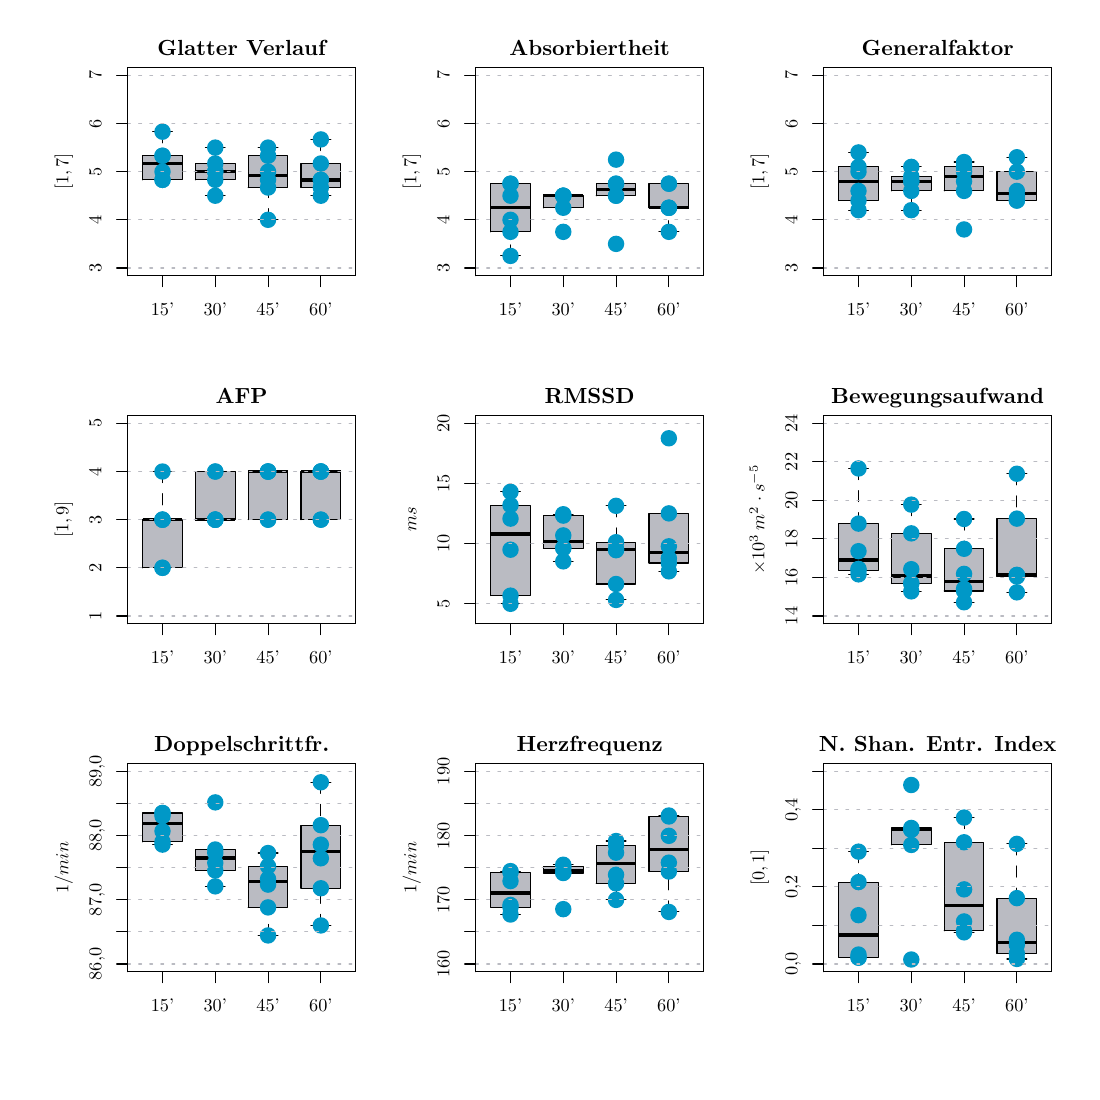
\begin{tikzpicture}[x=1pt,y=1pt]
\definecolor{fillColor}{RGB}{255,255,255}
\path[use as bounding box,fill=fillColor] (0,0) rectangle (377.25,377.25);
\begin{scope}
\path[clip] ( 36.13,287.63) rectangle (118.52,362.80);
\definecolor{fillColor}{RGB}{186,187,194}

\path[fill=fillColor] ( 41.57,322.26) --
	( 55.87,322.26) --
	( 55.87,330.96) --
	( 41.57,330.96) --
	cycle;
\definecolor{drawColor}{RGB}{0,0,0}

\path[draw=drawColor,line width= 1.2pt,line join=round] ( 41.57,328.09) -- ( 55.87,328.09);

\path[draw=drawColor,line width= 0.4pt,dash pattern=on 4pt off 4pt ,line join=round,line cap=round] ( 48.72,322.26) -- ( 48.72,322.26);

\path[draw=drawColor,line width= 0.4pt,dash pattern=on 4pt off 4pt ,line join=round,line cap=round] ( 48.72,339.66) -- ( 48.72,330.96);

\path[draw=drawColor,line width= 0.4pt,line join=round,line cap=round] ( 45.15,322.26) -- ( 52.30,322.26);

\path[draw=drawColor,line width= 0.4pt,line join=round,line cap=round] ( 45.15,339.66) -- ( 52.30,339.66);

\path[draw=drawColor,line width= 0.4pt,line join=round,line cap=round] ( 41.57,322.26) --
	( 55.87,322.26) --
	( 55.87,330.96) --
	( 41.57,330.96) --
	( 41.57,322.26);

\path[fill=fillColor] ( 60.64,322.26) --
	( 74.94,322.26) --
	( 74.94,328.17) --
	( 60.64,328.17) --
	cycle;

\path[draw=drawColor,line width= 1.2pt,line join=round] ( 60.64,325.21) -- ( 74.94,325.21);

\path[draw=drawColor,line width= 0.4pt,dash pattern=on 4pt off 4pt ,line join=round,line cap=round] ( 67.79,316.52) -- ( 67.79,322.26);

\path[draw=drawColor,line width= 0.4pt,dash pattern=on 4pt off 4pt ,line join=round,line cap=round] ( 67.79,333.91) -- ( 67.79,328.17);

\path[draw=drawColor,line width= 0.4pt,line join=round,line cap=round] ( 64.22,316.52) -- ( 71.37,316.52);

\path[draw=drawColor,line width= 0.4pt,line join=round,line cap=round] ( 64.22,333.91) -- ( 71.37,333.91);

\path[draw=drawColor,line width= 0.4pt,line join=round,line cap=round] ( 60.64,322.26) --
	( 74.94,322.26) --
	( 74.94,328.17) --
	( 60.64,328.17) --
	( 60.64,322.26);

\path[fill=fillColor] ( 79.71,319.47) --
	( 94.02,319.47) --
	( 94.02,330.96) --
	( 79.71,330.96) --
	cycle;

\path[draw=drawColor,line width= 1.2pt,line join=round] ( 79.71,323.74) -- ( 94.02,323.74);

\path[draw=drawColor,line width= 0.4pt,dash pattern=on 4pt off 4pt ,line join=round,line cap=round] ( 86.86,307.82) -- ( 86.86,319.47);

\path[draw=drawColor,line width= 0.4pt,dash pattern=on 4pt off 4pt ,line join=round,line cap=round] ( 86.86,333.91) -- ( 86.86,330.96);

\path[draw=drawColor,line width= 0.4pt,line join=round,line cap=round] ( 83.29,307.82) -- ( 90.44,307.82);

\path[draw=drawColor,line width= 0.4pt,line join=round,line cap=round] ( 83.29,333.91) -- ( 90.44,333.91);

\path[draw=drawColor,line width= 0.4pt,line join=round,line cap=round] ( 79.71,319.47) --
	( 94.02,319.47) --
	( 94.02,330.96) --
	( 79.71,330.96) --
	( 79.71,319.47);

\path[fill=fillColor] ( 98.78,319.47) --
	(113.09,319.47) --
	(113.09,328.17) --
	( 98.78,328.17) --
	cycle;

\path[draw=drawColor,line width= 1.2pt,line join=round] ( 98.78,322.26) -- (113.09,322.26);

\path[draw=drawColor,line width= 0.4pt,dash pattern=on 4pt off 4pt ,line join=round,line cap=round] (105.94,316.52) -- (105.94,319.47);

\path[draw=drawColor,line width= 0.4pt,dash pattern=on 4pt off 4pt ,line join=round,line cap=round] (105.94,336.87) -- (105.94,328.17);

\path[draw=drawColor,line width= 0.4pt,line join=round,line cap=round] (102.36,316.52) -- (109.51,316.52);

\path[draw=drawColor,line width= 0.4pt,line join=round,line cap=round] (102.36,336.87) -- (109.51,336.87);

\path[draw=drawColor,line width= 0.4pt,line join=round,line cap=round] ( 98.78,319.47) --
	(113.09,319.47) --
	(113.09,328.17) --
	( 98.78,328.17) --
	( 98.78,319.47);
\end{scope}
\begin{scope}
\path[clip] (  0.00,  0.00) rectangle (377.25,377.25);
\definecolor{drawColor}{RGB}{0,0,0}

\path[draw=drawColor,line width= 0.4pt,line join=round,line cap=round] ( 48.72,287.63) -- (105.94,287.63);

\path[draw=drawColor,line width= 0.4pt,line join=round,line cap=round] ( 48.72,287.63) -- ( 48.72,283.67);

\path[draw=drawColor,line width= 0.4pt,line join=round,line cap=round] ( 67.79,287.63) -- ( 67.79,283.67);

\path[draw=drawColor,line width= 0.4pt,line join=round,line cap=round] ( 86.86,287.63) -- ( 86.86,283.67);

\path[draw=drawColor,line width= 0.4pt,line join=round,line cap=round] (105.94,287.63) -- (105.94,283.67);

\node[text=drawColor,anchor=base,inner sep=0pt, outer sep=0pt, scale=  0.66] at ( 48.72,273.38) {15'};

\node[text=drawColor,anchor=base,inner sep=0pt, outer sep=0pt, scale=  0.66] at ( 67.79,273.38) {30'};

\node[text=drawColor,anchor=base,inner sep=0pt, outer sep=0pt, scale=  0.66] at ( 86.86,273.38) {45'};

\node[text=drawColor,anchor=base,inner sep=0pt, outer sep=0pt, scale=  0.66] at (105.94,273.38) {60'};

\path[draw=drawColor,line width= 0.4pt,line join=round,line cap=round] ( 36.13,290.42) -- ( 36.13,360.01);

\path[draw=drawColor,line width= 0.4pt,line join=round,line cap=round] ( 36.13,290.42) -- ( 32.17,290.42);

\path[draw=drawColor,line width= 0.4pt,line join=round,line cap=round] ( 36.13,307.82) -- ( 32.17,307.82);

\path[draw=drawColor,line width= 0.4pt,line join=round,line cap=round] ( 36.13,325.21) -- ( 32.17,325.21);

\path[draw=drawColor,line width= 0.4pt,line join=round,line cap=round] ( 36.13,342.61) -- ( 32.17,342.61);

\path[draw=drawColor,line width= 0.4pt,line join=round,line cap=round] ( 36.13,360.01) -- ( 32.17,360.01);

\node[text=drawColor,rotate= 90.00,anchor=base,inner sep=0pt, outer sep=0pt, scale=  0.66] at ( 26.63,290.42) {3};

\node[text=drawColor,rotate= 90.00,anchor=base,inner sep=0pt, outer sep=0pt, scale=  0.66] at ( 26.63,307.82) {4};

\node[text=drawColor,rotate= 90.00,anchor=base,inner sep=0pt, outer sep=0pt, scale=  0.66] at ( 26.63,325.21) {5};

\node[text=drawColor,rotate= 90.00,anchor=base,inner sep=0pt, outer sep=0pt, scale=  0.66] at ( 26.63,342.61) {6};

\node[text=drawColor,rotate= 90.00,anchor=base,inner sep=0pt, outer sep=0pt, scale=  0.66] at ( 26.63,360.01) {7};
\end{scope}
\begin{scope}
\path[clip] (  0.00,251.50) rectangle (125.75,377.25);
\definecolor{drawColor}{RGB}{0,0,0}

\node[text=drawColor,anchor=base,inner sep=0pt, outer sep=0pt, scale=  0.79] at ( 77.33,367.29) {\bfseries Glatter Verlauf};

\node[text=drawColor,rotate= 90.00,anchor=base,inner sep=0pt, outer sep=0pt, scale=  0.66] at ( 14.75,325.21) {$[1, 7]$};
\end{scope}
\begin{scope}
\path[clip] (  0.00,  0.00) rectangle (377.25,377.25);
\definecolor{drawColor}{RGB}{0,0,0}

\path[draw=drawColor,line width= 0.4pt,line join=round,line cap=round] ( 36.13,287.63) --
	(118.52,287.63) --
	(118.52,362.80) --
	( 36.13,362.80) --
	( 36.13,287.63);
\end{scope}
\begin{scope}
\path[clip] ( 36.13,287.63) rectangle (118.52,362.80);
\definecolor{fillColor}{RGB}{0,152,199}

\path[fill=fillColor] ( 48.72,325.21) circle (  2.97);

\path[fill=fillColor] ( 67.79,322.26) circle (  2.97);

\path[fill=fillColor] ( 86.86,319.47) circle (  2.97);

\path[fill=fillColor] (105.94,319.47) circle (  2.97);

\path[fill=fillColor] ( 48.72,322.26) circle (  2.97);

\path[fill=fillColor] ( 67.79,325.21) circle (  2.97);

\path[fill=fillColor] ( 86.86,325.21) circle (  2.97);

\path[fill=fillColor] (105.94,322.26) circle (  2.97);

\path[fill=fillColor] ( 48.72,322.26) circle (  2.97);

\path[fill=fillColor] ( 67.79,316.52) circle (  2.97);

\path[fill=fillColor] ( 86.86,307.82) circle (  2.97);

\path[fill=fillColor] (105.94,316.52) circle (  2.97);

\path[fill=fillColor] ( 48.72,330.96) circle (  2.97);

\path[fill=fillColor] ( 67.79,325.21) circle (  2.97);

\path[fill=fillColor] ( 86.86,333.91) circle (  2.97);

\path[fill=fillColor] (105.94,328.17) circle (  2.97);

\path[fill=fillColor] ( 48.72,330.96) circle (  2.97);

\path[fill=fillColor] ( 67.79,328.17) circle (  2.97);

\path[fill=fillColor] ( 86.86,330.96) circle (  2.97);

\path[fill=fillColor] (105.94,336.87) circle (  2.97);

\path[fill=fillColor] ( 48.72,339.66) circle (  2.97);

\path[fill=fillColor] ( 67.79,333.91) circle (  2.97);

\path[fill=fillColor] ( 86.86,322.26) circle (  2.97);

\path[fill=fillColor] (105.94,322.26) circle (  2.97);
\definecolor{drawColor}{RGB}{186,187,194}

\path[draw=drawColor,line width= 0.4pt,dash pattern=on 1pt off 3pt ,line join=round,line cap=round] ( 36.13,290.42) -- (118.52,290.42);

\path[draw=drawColor,line width= 0.4pt,dash pattern=on 1pt off 3pt ,line join=round,line cap=round] ( 36.13,307.82) -- (118.52,307.82);

\path[draw=drawColor,line width= 0.4pt,dash pattern=on 1pt off 3pt ,line join=round,line cap=round] ( 36.13,325.21) -- (118.52,325.21);

\path[draw=drawColor,line width= 0.4pt,dash pattern=on 1pt off 3pt ,line join=round,line cap=round] ( 36.13,342.61) -- (118.52,342.61);

\path[draw=drawColor,line width= 0.4pt,dash pattern=on 1pt off 3pt ,line join=round,line cap=round] ( 36.13,360.01) -- (118.52,360.01);
\end{scope}
\begin{scope}
\path[clip] (  0.00,  0.00) rectangle (377.25,377.25);
\definecolor{drawColor}{RGB}{0,0,0}

\path[draw=drawColor,line width= 0.4pt,line join=round,line cap=round] ( 36.13,287.63) --
	(118.52,287.63) --
	(118.52,362.80) --
	( 36.13,362.80) --
	( 36.13,287.63);
\end{scope}
\begin{scope}
\path[clip] (161.88,287.63) rectangle (244.27,362.80);
\definecolor{fillColor}{RGB}{186,187,194}

\path[fill=fillColor] (167.32,303.47) --
	(181.62,303.47) --
	(181.62,320.87) --
	(167.32,320.87) --
	cycle;
\definecolor{drawColor}{RGB}{0,0,0}

\path[draw=drawColor,line width= 1.2pt,line join=round] (167.32,312.17) -- (181.62,312.17);

\path[draw=drawColor,line width= 0.4pt,dash pattern=on 4pt off 4pt ,line join=round,line cap=round] (174.47,294.77) -- (174.47,303.47);

\path[draw=drawColor,line width= 0.4pt,dash pattern=on 4pt off 4pt ,line join=round,line cap=round] (174.47,320.87) -- (174.47,320.87);

\path[draw=drawColor,line width= 0.4pt,line join=round,line cap=round] (170.90,294.77) -- (178.05,294.77);

\path[draw=drawColor,line width= 0.4pt,line join=round,line cap=round] (170.90,320.87) -- (178.05,320.87);

\path[draw=drawColor,line width= 0.4pt,line join=round,line cap=round] (167.32,303.47) --
	(181.62,303.47) --
	(181.62,320.87) --
	(167.32,320.87) --
	(167.32,303.47);

\path[fill=fillColor] (186.39,312.17) --
	(200.69,312.17) --
	(200.69,316.52) --
	(186.39,316.52) --
	cycle;

\path[draw=drawColor,line width= 1.2pt,line join=round] (186.39,316.52) -- (200.69,316.52);

\path[draw=drawColor,line width= 0.4pt,dash pattern=on 4pt off 4pt ,line join=round,line cap=round] (193.54,312.17) -- (193.54,312.17);

\path[draw=drawColor,line width= 0.4pt,dash pattern=on 4pt off 4pt ,line join=round,line cap=round] (193.54,316.52) -- (193.54,316.52);

\path[draw=drawColor,line width= 0.4pt,line join=round,line cap=round] (189.97,312.17) -- (197.12,312.17);

\path[draw=drawColor,line width= 0.4pt,line join=round,line cap=round] (189.97,316.52) -- (197.12,316.52);

\path[draw=drawColor,line width= 0.4pt,line join=round,line cap=round] (186.39,312.17) --
	(200.69,312.17) --
	(200.69,316.52) --
	(186.39,316.52) --
	(186.39,312.17);

\path[fill=fillColor] (205.46,316.52) --
	(219.77,316.52) --
	(219.77,320.87) --
	(205.46,320.87) --
	cycle;

\path[draw=drawColor,line width= 1.2pt,line join=round] (205.46,318.69) -- (219.77,318.69);

\path[draw=drawColor,line width= 0.4pt,dash pattern=on 4pt off 4pt ,line join=round,line cap=round] (212.61,316.52) -- (212.61,316.52);

\path[draw=drawColor,line width= 0.4pt,dash pattern=on 4pt off 4pt ,line join=round,line cap=round] (212.61,320.87) -- (212.61,320.87);

\path[draw=drawColor,line width= 0.4pt,line join=round,line cap=round] (209.04,316.52) -- (216.19,316.52);

\path[draw=drawColor,line width= 0.4pt,line join=round,line cap=round] (209.04,320.87) -- (216.19,320.87);

\path[draw=drawColor,line width= 0.4pt,line join=round,line cap=round] (205.46,316.52) --
	(219.77,316.52) --
	(219.77,320.87) --
	(205.46,320.87) --
	(205.46,316.52);

\path[fill=fillColor] (224.53,312.17) --
	(238.84,312.17) --
	(238.84,320.87) --
	(224.53,320.87) --
	cycle;

\path[draw=drawColor,line width= 1.2pt,line join=round] (224.53,312.17) -- (238.84,312.17);

\path[draw=drawColor,line width= 0.4pt,dash pattern=on 4pt off 4pt ,line join=round,line cap=round] (231.69,303.47) -- (231.69,312.17);

\path[draw=drawColor,line width= 0.4pt,dash pattern=on 4pt off 4pt ,line join=round,line cap=round] (231.69,320.87) -- (231.69,320.87);

\path[draw=drawColor,line width= 0.4pt,line join=round,line cap=round] (228.11,303.47) -- (235.26,303.47);

\path[draw=drawColor,line width= 0.4pt,line join=round,line cap=round] (228.11,320.87) -- (235.26,320.87);

\path[draw=drawColor,line width= 0.4pt,line join=round,line cap=round] (224.53,312.17) --
	(238.84,312.17) --
	(238.84,320.87) --
	(224.53,320.87) --
	(224.53,312.17);
\end{scope}
\begin{scope}
\path[clip] (  0.00,  0.00) rectangle (377.25,377.25);
\definecolor{drawColor}{RGB}{0,0,0}

\path[draw=drawColor,line width= 0.4pt,line join=round,line cap=round] (174.47,287.63) -- (231.69,287.63);

\path[draw=drawColor,line width= 0.4pt,line join=round,line cap=round] (174.47,287.63) -- (174.47,283.67);

\path[draw=drawColor,line width= 0.4pt,line join=round,line cap=round] (193.54,287.63) -- (193.54,283.67);

\path[draw=drawColor,line width= 0.4pt,line join=round,line cap=round] (212.61,287.63) -- (212.61,283.67);

\path[draw=drawColor,line width= 0.4pt,line join=round,line cap=round] (231.69,287.63) -- (231.69,283.67);

\node[text=drawColor,anchor=base,inner sep=0pt, outer sep=0pt, scale=  0.66] at (174.47,273.38) {15'};

\node[text=drawColor,anchor=base,inner sep=0pt, outer sep=0pt, scale=  0.66] at (193.54,273.38) {30'};

\node[text=drawColor,anchor=base,inner sep=0pt, outer sep=0pt, scale=  0.66] at (212.61,273.38) {45'};

\node[text=drawColor,anchor=base,inner sep=0pt, outer sep=0pt, scale=  0.66] at (231.69,273.38) {60'};

\path[draw=drawColor,line width= 0.4pt,line join=round,line cap=round] (161.88,290.42) -- (161.88,360.01);

\path[draw=drawColor,line width= 0.4pt,line join=round,line cap=round] (161.88,290.42) -- (157.92,290.42);

\path[draw=drawColor,line width= 0.4pt,line join=round,line cap=round] (161.88,307.82) -- (157.92,307.82);

\path[draw=drawColor,line width= 0.4pt,line join=round,line cap=round] (161.88,325.21) -- (157.92,325.21);

\path[draw=drawColor,line width= 0.4pt,line join=round,line cap=round] (161.88,342.61) -- (157.92,342.61);

\path[draw=drawColor,line width= 0.4pt,line join=round,line cap=round] (161.88,360.01) -- (157.92,360.01);

\node[text=drawColor,rotate= 90.00,anchor=base,inner sep=0pt, outer sep=0pt, scale=  0.66] at (152.38,290.42) {3};

\node[text=drawColor,rotate= 90.00,anchor=base,inner sep=0pt, outer sep=0pt, scale=  0.66] at (152.38,307.82) {4};

\node[text=drawColor,rotate= 90.00,anchor=base,inner sep=0pt, outer sep=0pt, scale=  0.66] at (152.38,325.21) {5};

\node[text=drawColor,rotate= 90.00,anchor=base,inner sep=0pt, outer sep=0pt, scale=  0.66] at (152.38,342.61) {6};

\node[text=drawColor,rotate= 90.00,anchor=base,inner sep=0pt, outer sep=0pt, scale=  0.66] at (152.38,360.01) {7};
\end{scope}
\begin{scope}
\path[clip] (125.75,251.50) rectangle (251.50,377.25);
\definecolor{drawColor}{RGB}{0,0,0}

\node[text=drawColor,anchor=base,inner sep=0pt, outer sep=0pt, scale=  0.79] at (203.08,367.29) {\bfseries Absorbiertheit};

\node[text=drawColor,rotate= 90.00,anchor=base,inner sep=0pt, outer sep=0pt, scale=  0.66] at (140.50,325.21) {$[1, 7]$};
\end{scope}
\begin{scope}
\path[clip] (  0.00,  0.00) rectangle (377.25,377.25);
\definecolor{drawColor}{RGB}{0,0,0}

\path[draw=drawColor,line width= 0.4pt,line join=round,line cap=round] (161.88,287.63) --
	(244.27,287.63) --
	(244.27,362.80) --
	(161.88,362.80) --
	(161.88,287.63);
\end{scope}
\begin{scope}
\path[clip] (161.88,287.63) rectangle (244.27,362.80);
\definecolor{fillColor}{RGB}{0,152,199}

\path[fill=fillColor] (174.47,307.82) circle (  2.97);

\path[fill=fillColor] (193.54,312.17) circle (  2.97);

\path[fill=fillColor] (212.61,316.52) circle (  2.97);

\path[fill=fillColor] (231.69,312.17) circle (  2.97);

\path[fill=fillColor] (174.47,294.77) circle (  2.97);

\path[fill=fillColor] (193.54,316.52) circle (  2.97);

\path[fill=fillColor] (212.61,316.52) circle (  2.97);

\path[fill=fillColor] (231.69,312.17) circle (  2.97);

\path[fill=fillColor] (174.47,303.47) circle (  2.97);

\path[fill=fillColor] (193.54,303.47) circle (  2.97);

\path[fill=fillColor] (212.61,299.12) circle (  2.97);

\path[fill=fillColor] (231.69,312.17) circle (  2.97);

\path[fill=fillColor] (174.47,316.52) circle (  2.97);

\path[fill=fillColor] (193.54,316.52) circle (  2.97);

\path[fill=fillColor] (212.61,320.87) circle (  2.97);

\path[fill=fillColor] (231.69,320.87) circle (  2.97);

\path[fill=fillColor] (174.47,320.87) circle (  2.97);

\path[fill=fillColor] (193.54,316.52) circle (  2.97);

\path[fill=fillColor] (212.61,320.87) circle (  2.97);

\path[fill=fillColor] (231.69,320.87) circle (  2.97);

\path[fill=fillColor] (174.47,320.87) circle (  2.97);

\path[fill=fillColor] (193.54,316.52) circle (  2.97);

\path[fill=fillColor] (212.61,329.56) circle (  2.97);

\path[fill=fillColor] (231.69,303.47) circle (  2.97);
\definecolor{drawColor}{RGB}{186,187,194}

\path[draw=drawColor,line width= 0.4pt,dash pattern=on 1pt off 3pt ,line join=round,line cap=round] (161.88,290.42) -- (244.27,290.42);

\path[draw=drawColor,line width= 0.4pt,dash pattern=on 1pt off 3pt ,line join=round,line cap=round] (161.88,307.82) -- (244.27,307.82);

\path[draw=drawColor,line width= 0.4pt,dash pattern=on 1pt off 3pt ,line join=round,line cap=round] (161.88,325.21) -- (244.27,325.21);

\path[draw=drawColor,line width= 0.4pt,dash pattern=on 1pt off 3pt ,line join=round,line cap=round] (161.88,342.61) -- (244.27,342.61);

\path[draw=drawColor,line width= 0.4pt,dash pattern=on 1pt off 3pt ,line join=round,line cap=round] (161.88,360.01) -- (244.27,360.01);
\end{scope}
\begin{scope}
\path[clip] (  0.00,  0.00) rectangle (377.25,377.25);
\definecolor{drawColor}{RGB}{0,0,0}

\path[draw=drawColor,line width= 0.4pt,line join=round,line cap=round] (161.88,287.63) --
	(244.27,287.63) --
	(244.27,362.80) --
	(161.88,362.80) --
	(161.88,287.63);
\end{scope}
\begin{scope}
\path[clip] (287.63,287.63) rectangle (370.02,362.80);
\definecolor{fillColor}{RGB}{186,187,194}

\path[fill=fillColor] (293.07,314.78) --
	(307.37,314.78) --
	(307.37,326.95) --
	(293.07,326.95) --
	cycle;
\definecolor{drawColor}{RGB}{0,0,0}

\path[draw=drawColor,line width= 1.2pt,line join=round] (293.07,321.74) -- (307.37,321.74);

\path[draw=drawColor,line width= 0.4pt,dash pattern=on 4pt off 4pt ,line join=round,line cap=round] (300.22,311.30) -- (300.22,314.78);

\path[draw=drawColor,line width= 0.4pt,dash pattern=on 4pt off 4pt ,line join=round,line cap=round] (300.22,332.17) -- (300.22,326.95);

\path[draw=drawColor,line width= 0.4pt,line join=round,line cap=round] (296.65,311.30) -- (303.80,311.30);

\path[draw=drawColor,line width= 0.4pt,line join=round,line cap=round] (296.65,332.17) -- (303.80,332.17);

\path[draw=drawColor,line width= 0.4pt,line join=round,line cap=round] (293.07,314.78) --
	(307.37,314.78) --
	(307.37,326.95) --
	(293.07,326.95) --
	(293.07,314.78);

\path[fill=fillColor] (312.14,318.26) --
	(326.44,318.26) --
	(326.44,323.48) --
	(312.14,323.48) --
	cycle;

\path[draw=drawColor,line width= 1.2pt,line join=round] (312.14,321.74) -- (326.44,321.74);

\path[draw=drawColor,line width= 0.4pt,dash pattern=on 4pt off 4pt ,line join=round,line cap=round] (319.29,311.30) -- (319.29,318.26);

\path[draw=drawColor,line width= 0.4pt,dash pattern=on 4pt off 4pt ,line join=round,line cap=round] (319.29,326.95) -- (319.29,323.48);

\path[draw=drawColor,line width= 0.4pt,line join=round,line cap=round] (315.72,311.30) -- (322.87,311.30);

\path[draw=drawColor,line width= 0.4pt,line join=round,line cap=round] (315.72,326.95) -- (322.87,326.95);

\path[draw=drawColor,line width= 0.4pt,line join=round,line cap=round] (312.14,318.26) --
	(326.44,318.26) --
	(326.44,323.48) --
	(312.14,323.48) --
	(312.14,318.26);

\path[fill=fillColor] (331.21,318.26) --
	(345.52,318.26) --
	(345.52,326.95) --
	(331.21,326.95) --
	cycle;

\path[draw=drawColor,line width= 1.2pt,line join=round] (331.21,323.48) -- (345.52,323.48);

\path[draw=drawColor,line width= 0.4pt,dash pattern=on 4pt off 4pt ,line join=round,line cap=round] (338.36,318.26) -- (338.36,318.26);

\path[draw=drawColor,line width= 0.4pt,dash pattern=on 4pt off 4pt ,line join=round,line cap=round] (338.36,328.69) -- (338.36,326.95);

\path[draw=drawColor,line width= 0.4pt,line join=round,line cap=round] (334.79,318.26) -- (341.94,318.26);

\path[draw=drawColor,line width= 0.4pt,line join=round,line cap=round] (334.79,328.69) -- (341.94,328.69);

\path[draw=drawColor,line width= 0.4pt,line join=round,line cap=round] (331.21,318.26) --
	(345.52,318.26) --
	(345.52,326.95) --
	(331.21,326.95) --
	(331.21,318.26);

\path[fill=fillColor] (350.28,314.78) --
	(364.59,314.78) --
	(364.59,325.21) --
	(350.28,325.21) --
	cycle;

\path[draw=drawColor,line width= 1.2pt,line join=round] (350.28,317.39) -- (364.59,317.39);

\path[draw=drawColor,line width= 0.4pt,dash pattern=on 4pt off 4pt ,line join=round,line cap=round] (357.44,314.78) -- (357.44,314.78);

\path[draw=drawColor,line width= 0.4pt,dash pattern=on 4pt off 4pt ,line join=round,line cap=round] (357.44,330.43) -- (357.44,325.21);

\path[draw=drawColor,line width= 0.4pt,line join=round,line cap=round] (353.86,314.78) -- (361.01,314.78);

\path[draw=drawColor,line width= 0.4pt,line join=round,line cap=round] (353.86,330.43) -- (361.01,330.43);

\path[draw=drawColor,line width= 0.4pt,line join=round,line cap=round] (350.28,314.78) --
	(364.59,314.78) --
	(364.59,325.21) --
	(350.28,325.21) --
	(350.28,314.78);
\end{scope}
\begin{scope}
\path[clip] (  0.00,  0.00) rectangle (377.25,377.25);
\definecolor{drawColor}{RGB}{0,0,0}

\path[draw=drawColor,line width= 0.4pt,line join=round,line cap=round] (300.22,287.63) -- (357.44,287.63);

\path[draw=drawColor,line width= 0.4pt,line join=round,line cap=round] (300.22,287.63) -- (300.22,283.67);

\path[draw=drawColor,line width= 0.4pt,line join=round,line cap=round] (319.29,287.63) -- (319.29,283.67);

\path[draw=drawColor,line width= 0.4pt,line join=round,line cap=round] (338.36,287.63) -- (338.36,283.67);

\path[draw=drawColor,line width= 0.4pt,line join=round,line cap=round] (357.44,287.63) -- (357.44,283.67);

\node[text=drawColor,anchor=base,inner sep=0pt, outer sep=0pt, scale=  0.66] at (300.22,273.38) {15'};

\node[text=drawColor,anchor=base,inner sep=0pt, outer sep=0pt, scale=  0.66] at (319.29,273.38) {30'};

\node[text=drawColor,anchor=base,inner sep=0pt, outer sep=0pt, scale=  0.66] at (338.36,273.38) {45'};

\node[text=drawColor,anchor=base,inner sep=0pt, outer sep=0pt, scale=  0.66] at (357.44,273.38) {60'};

\path[draw=drawColor,line width= 0.4pt,line join=round,line cap=round] (287.63,290.42) -- (287.63,360.01);

\path[draw=drawColor,line width= 0.4pt,line join=round,line cap=round] (287.63,290.42) -- (283.67,290.42);

\path[draw=drawColor,line width= 0.4pt,line join=round,line cap=round] (287.63,307.82) -- (283.67,307.82);

\path[draw=drawColor,line width= 0.4pt,line join=round,line cap=round] (287.63,325.21) -- (283.67,325.21);

\path[draw=drawColor,line width= 0.4pt,line join=round,line cap=round] (287.63,342.61) -- (283.67,342.61);

\path[draw=drawColor,line width= 0.4pt,line join=round,line cap=round] (287.63,360.01) -- (283.67,360.01);

\node[text=drawColor,rotate= 90.00,anchor=base,inner sep=0pt, outer sep=0pt, scale=  0.66] at (278.13,290.42) {3};

\node[text=drawColor,rotate= 90.00,anchor=base,inner sep=0pt, outer sep=0pt, scale=  0.66] at (278.13,307.82) {4};

\node[text=drawColor,rotate= 90.00,anchor=base,inner sep=0pt, outer sep=0pt, scale=  0.66] at (278.13,325.21) {5};

\node[text=drawColor,rotate= 90.00,anchor=base,inner sep=0pt, outer sep=0pt, scale=  0.66] at (278.13,342.61) {6};

\node[text=drawColor,rotate= 90.00,anchor=base,inner sep=0pt, outer sep=0pt, scale=  0.66] at (278.13,360.01) {7};
\end{scope}
\begin{scope}
\path[clip] (251.50,251.50) rectangle (377.25,377.25);
\definecolor{drawColor}{RGB}{0,0,0}

\node[text=drawColor,anchor=base,inner sep=0pt, outer sep=0pt, scale=  0.79] at (328.83,367.29) {\bfseries Generalfaktor};

\node[text=drawColor,rotate= 90.00,anchor=base,inner sep=0pt, outer sep=0pt, scale=  0.66] at (266.25,325.21) {$[1, 7]$};
\end{scope}
\begin{scope}
\path[clip] (  0.00,  0.00) rectangle (377.25,377.25);
\definecolor{drawColor}{RGB}{0,0,0}

\path[draw=drawColor,line width= 0.4pt,line join=round,line cap=round] (287.63,287.63) --
	(370.02,287.63) --
	(370.02,362.80) --
	(287.63,362.80) --
	(287.63,287.63);
\end{scope}
\begin{scope}
\path[clip] (287.63,287.63) rectangle (370.02,362.80);
\definecolor{fillColor}{RGB}{0,152,199}

\path[fill=fillColor] (300.22,318.26) circle (  2.97);

\path[fill=fillColor] (319.29,318.26) circle (  2.97);

\path[fill=fillColor] (338.36,318.26) circle (  2.97);

\path[fill=fillColor] (357.44,316.52) circle (  2.97);

\path[fill=fillColor] (300.22,311.30) circle (  2.97);

\path[fill=fillColor] (319.29,321.74) circle (  2.97);

\path[fill=fillColor] (338.36,321.74) circle (  2.97);

\path[fill=fillColor] (357.44,318.26) circle (  2.97);

\path[fill=fillColor] (300.22,314.78) circle (  2.97);

\path[fill=fillColor] (319.29,311.30) circle (  2.97);

\path[fill=fillColor] (338.36,304.34) circle (  2.97);

\path[fill=fillColor] (357.44,314.78) circle (  2.97);

\path[fill=fillColor] (300.22,325.21) circle (  2.97);

\path[fill=fillColor] (319.29,321.74) circle (  2.97);

\path[fill=fillColor] (338.36,328.69) circle (  2.97);

\path[fill=fillColor] (357.44,325.21) circle (  2.97);

\path[fill=fillColor] (300.22,326.95) circle (  2.97);

\path[fill=fillColor] (319.29,323.48) circle (  2.97);

\path[fill=fillColor] (338.36,326.95) circle (  2.97);

\path[fill=fillColor] (357.44,330.43) circle (  2.97);

\path[fill=fillColor] (300.22,332.17) circle (  2.97);

\path[fill=fillColor] (319.29,326.95) circle (  2.97);

\path[fill=fillColor] (338.36,325.21) circle (  2.97);

\path[fill=fillColor] (357.44,314.78) circle (  2.97);
\definecolor{drawColor}{RGB}{186,187,194}

\path[draw=drawColor,line width= 0.4pt,dash pattern=on 1pt off 3pt ,line join=round,line cap=round] (287.63,290.42) -- (370.02,290.42);

\path[draw=drawColor,line width= 0.4pt,dash pattern=on 1pt off 3pt ,line join=round,line cap=round] (287.63,307.82) -- (370.02,307.82);

\path[draw=drawColor,line width= 0.4pt,dash pattern=on 1pt off 3pt ,line join=round,line cap=round] (287.63,325.21) -- (370.02,325.21);

\path[draw=drawColor,line width= 0.4pt,dash pattern=on 1pt off 3pt ,line join=round,line cap=round] (287.63,342.61) -- (370.02,342.61);

\path[draw=drawColor,line width= 0.4pt,dash pattern=on 1pt off 3pt ,line join=round,line cap=round] (287.63,360.01) -- (370.02,360.01);
\end{scope}
\begin{scope}
\path[clip] (  0.00,  0.00) rectangle (377.25,377.25);
\definecolor{drawColor}{RGB}{0,0,0}

\path[draw=drawColor,line width= 0.4pt,line join=round,line cap=round] (287.63,287.63) --
	(370.02,287.63) --
	(370.02,362.80) --
	(287.63,362.80) --
	(287.63,287.63);
\end{scope}
\begin{scope}
\path[clip] ( 36.13,161.88) rectangle (118.52,237.05);
\definecolor{fillColor}{RGB}{186,187,194}

\path[fill=fillColor] ( 41.57,182.07) --
	( 55.87,182.07) --
	( 55.87,199.47) --
	( 41.57,199.47) --
	cycle;
\definecolor{drawColor}{RGB}{0,0,0}

\path[draw=drawColor,line width= 1.2pt,line join=round] ( 41.57,199.47) -- ( 55.87,199.47);

\path[draw=drawColor,line width= 0.4pt,dash pattern=on 4pt off 4pt ,line join=round,line cap=round] ( 48.72,182.07) -- ( 48.72,182.07);

\path[draw=drawColor,line width= 0.4pt,dash pattern=on 4pt off 4pt ,line join=round,line cap=round] ( 48.72,216.86) -- ( 48.72,199.47);

\path[draw=drawColor,line width= 0.4pt,line join=round,line cap=round] ( 45.15,182.07) -- ( 52.30,182.07);

\path[draw=drawColor,line width= 0.4pt,line join=round,line cap=round] ( 45.15,216.86) -- ( 52.30,216.86);

\path[draw=drawColor,line width= 0.4pt,line join=round,line cap=round] ( 41.57,182.07) --
	( 55.87,182.07) --
	( 55.87,199.47) --
	( 41.57,199.47) --
	( 41.57,182.07);

\path[fill=fillColor] ( 60.64,199.47) --
	( 74.94,199.47) --
	( 74.94,216.86) --
	( 60.64,216.86) --
	cycle;

\path[draw=drawColor,line width= 1.2pt,line join=round] ( 60.64,199.47) -- ( 74.94,199.47);

\path[draw=drawColor,line width= 0.4pt,dash pattern=on 4pt off 4pt ,line join=round,line cap=round] ( 67.79,199.47) -- ( 67.79,199.47);

\path[draw=drawColor,line width= 0.4pt,dash pattern=on 4pt off 4pt ,line join=round,line cap=round] ( 67.79,216.86) -- ( 67.79,216.86);

\path[draw=drawColor,line width= 0.4pt,line join=round,line cap=round] ( 64.22,199.47) -- ( 71.37,199.47);

\path[draw=drawColor,line width= 0.4pt,line join=round,line cap=round] ( 64.22,216.86) -- ( 71.37,216.86);

\path[draw=drawColor,line width= 0.4pt,line join=round,line cap=round] ( 60.64,199.47) --
	( 74.94,199.47) --
	( 74.94,216.86) --
	( 60.64,216.86) --
	( 60.64,199.47);

\path[fill=fillColor] ( 79.71,199.47) --
	( 94.02,199.47) --
	( 94.02,216.86) --
	( 79.71,216.86) --
	cycle;

\path[draw=drawColor,line width= 1.2pt,line join=round] ( 79.71,216.86) -- ( 94.02,216.86);

\path[draw=drawColor,line width= 0.4pt,dash pattern=on 4pt off 4pt ,line join=round,line cap=round] ( 86.86,199.47) -- ( 86.86,199.47);

\path[draw=drawColor,line width= 0.4pt,dash pattern=on 4pt off 4pt ,line join=round,line cap=round] ( 86.86,216.86) -- ( 86.86,216.86);

\path[draw=drawColor,line width= 0.4pt,line join=round,line cap=round] ( 83.29,199.47) -- ( 90.44,199.47);

\path[draw=drawColor,line width= 0.4pt,line join=round,line cap=round] ( 83.29,216.86) -- ( 90.44,216.86);

\path[draw=drawColor,line width= 0.4pt,line join=round,line cap=round] ( 79.71,199.47) --
	( 94.02,199.47) --
	( 94.02,216.86) --
	( 79.71,216.86) --
	( 79.71,199.47);

\path[fill=fillColor] ( 98.78,199.47) --
	(113.09,199.47) --
	(113.09,216.86) --
	( 98.78,216.86) --
	cycle;

\path[draw=drawColor,line width= 1.2pt,line join=round] ( 98.78,216.86) -- (113.09,216.86);

\path[draw=drawColor,line width= 0.4pt,dash pattern=on 4pt off 4pt ,line join=round,line cap=round] (105.94,199.47) -- (105.94,199.47);

\path[draw=drawColor,line width= 0.4pt,dash pattern=on 4pt off 4pt ,line join=round,line cap=round] (105.94,216.86) -- (105.94,216.86);

\path[draw=drawColor,line width= 0.4pt,line join=round,line cap=round] (102.36,199.47) -- (109.51,199.47);

\path[draw=drawColor,line width= 0.4pt,line join=round,line cap=round] (102.36,216.86) -- (109.51,216.86);

\path[draw=drawColor,line width= 0.4pt,line join=round,line cap=round] ( 98.78,199.47) --
	(113.09,199.47) --
	(113.09,216.86) --
	( 98.78,216.86) --
	( 98.78,199.47);
\end{scope}
\begin{scope}
\path[clip] (  0.00,  0.00) rectangle (377.25,377.25);
\definecolor{drawColor}{RGB}{0,0,0}

\path[draw=drawColor,line width= 0.4pt,line join=round,line cap=round] ( 48.72,161.88) -- (105.94,161.88);

\path[draw=drawColor,line width= 0.4pt,line join=round,line cap=round] ( 48.72,161.88) -- ( 48.72,157.92);

\path[draw=drawColor,line width= 0.4pt,line join=round,line cap=round] ( 67.79,161.88) -- ( 67.79,157.92);

\path[draw=drawColor,line width= 0.4pt,line join=round,line cap=round] ( 86.86,161.88) -- ( 86.86,157.92);

\path[draw=drawColor,line width= 0.4pt,line join=round,line cap=round] (105.94,161.88) -- (105.94,157.92);

\node[text=drawColor,anchor=base,inner sep=0pt, outer sep=0pt, scale=  0.66] at ( 48.72,147.63) {15'};

\node[text=drawColor,anchor=base,inner sep=0pt, outer sep=0pt, scale=  0.66] at ( 67.79,147.63) {30'};

\node[text=drawColor,anchor=base,inner sep=0pt, outer sep=0pt, scale=  0.66] at ( 86.86,147.63) {45'};

\node[text=drawColor,anchor=base,inner sep=0pt, outer sep=0pt, scale=  0.66] at (105.94,147.63) {60'};

\path[draw=drawColor,line width= 0.4pt,line join=round,line cap=round] ( 36.13,164.67) -- ( 36.13,234.26);

\path[draw=drawColor,line width= 0.4pt,line join=round,line cap=round] ( 36.13,164.67) -- ( 32.17,164.67);

\path[draw=drawColor,line width= 0.4pt,line join=round,line cap=round] ( 36.13,182.07) -- ( 32.17,182.07);

\path[draw=drawColor,line width= 0.4pt,line join=round,line cap=round] ( 36.13,199.47) -- ( 32.17,199.47);

\path[draw=drawColor,line width= 0.4pt,line join=round,line cap=round] ( 36.13,216.86) -- ( 32.17,216.86);

\path[draw=drawColor,line width= 0.4pt,line join=round,line cap=round] ( 36.13,234.26) -- ( 32.17,234.26);

\node[text=drawColor,rotate= 90.00,anchor=base,inner sep=0pt, outer sep=0pt, scale=  0.66] at ( 26.63,164.67) {1};

\node[text=drawColor,rotate= 90.00,anchor=base,inner sep=0pt, outer sep=0pt, scale=  0.66] at ( 26.63,182.07) {2};

\node[text=drawColor,rotate= 90.00,anchor=base,inner sep=0pt, outer sep=0pt, scale=  0.66] at ( 26.63,199.47) {3};

\node[text=drawColor,rotate= 90.00,anchor=base,inner sep=0pt, outer sep=0pt, scale=  0.66] at ( 26.63,216.86) {4};

\node[text=drawColor,rotate= 90.00,anchor=base,inner sep=0pt, outer sep=0pt, scale=  0.66] at ( 26.63,234.26) {5};
\end{scope}
\begin{scope}
\path[clip] (  0.00,125.75) rectangle (125.75,251.50);
\definecolor{drawColor}{RGB}{0,0,0}

\node[text=drawColor,anchor=base,inner sep=0pt, outer sep=0pt, scale=  0.79] at ( 77.33,241.54) {\bfseries AFP};

\node[text=drawColor,rotate= 90.00,anchor=base,inner sep=0pt, outer sep=0pt, scale=  0.66] at ( 14.75,199.47) {$[1, 9]$};
\end{scope}
\begin{scope}
\path[clip] (  0.00,  0.00) rectangle (377.25,377.25);
\definecolor{drawColor}{RGB}{0,0,0}

\path[draw=drawColor,line width= 0.4pt,line join=round,line cap=round] ( 36.13,161.88) --
	(118.52,161.88) --
	(118.52,237.05) --
	( 36.13,237.05) --
	( 36.13,161.88);
\end{scope}
\begin{scope}
\path[clip] ( 36.13,161.88) rectangle (118.52,237.05);
\definecolor{fillColor}{RGB}{0,152,199}

\path[fill=fillColor] ( 48.72,182.07) circle (  2.97);

\path[fill=fillColor] ( 67.79,199.47) circle (  2.97);

\path[fill=fillColor] ( 86.86,199.47) circle (  2.97);

\path[fill=fillColor] (105.94,199.47) circle (  2.97);

\path[fill=fillColor] ( 48.72,182.07) circle (  2.97);

\path[fill=fillColor] ( 67.79,199.47) circle (  2.97);

\path[fill=fillColor] ( 86.86,199.47) circle (  2.97);

\path[fill=fillColor] (105.94,199.47) circle (  2.97);

\path[fill=fillColor] ( 48.72,199.47) circle (  2.97);

\path[fill=fillColor] ( 67.79,216.86) circle (  2.97);

\path[fill=fillColor] ( 86.86,216.86) circle (  2.97);

\path[fill=fillColor] (105.94,216.86) circle (  2.97);

\path[fill=fillColor] ( 48.72,216.86) circle (  2.97);

\path[fill=fillColor] ( 67.79,216.86) circle (  2.97);

\path[fill=fillColor] ( 86.86,216.86) circle (  2.97);

\path[fill=fillColor] (105.94,216.86) circle (  2.97);

\path[fill=fillColor] ( 48.72,199.47) circle (  2.97);

\path[fill=fillColor] ( 67.79,199.47) circle (  2.97);

\path[fill=fillColor] ( 86.86,216.86) circle (  2.97);

\path[fill=fillColor] (105.94,216.86) circle (  2.97);

\path[fill=fillColor] ( 48.72,199.47) circle (  2.97);

\path[fill=fillColor] ( 67.79,199.47) circle (  2.97);

\path[fill=fillColor] ( 86.86,216.86) circle (  2.97);

\path[fill=fillColor] (105.94,216.86) circle (  2.97);
\definecolor{drawColor}{RGB}{186,187,194}

\path[draw=drawColor,line width= 0.4pt,dash pattern=on 1pt off 3pt ,line join=round,line cap=round] ( 36.13,164.67) -- (118.52,164.67);

\path[draw=drawColor,line width= 0.4pt,dash pattern=on 1pt off 3pt ,line join=round,line cap=round] ( 36.13,182.07) -- (118.52,182.07);

\path[draw=drawColor,line width= 0.4pt,dash pattern=on 1pt off 3pt ,line join=round,line cap=round] ( 36.13,199.47) -- (118.52,199.47);

\path[draw=drawColor,line width= 0.4pt,dash pattern=on 1pt off 3pt ,line join=round,line cap=round] ( 36.13,216.86) -- (118.52,216.86);

\path[draw=drawColor,line width= 0.4pt,dash pattern=on 1pt off 3pt ,line join=round,line cap=round] ( 36.13,234.26) -- (118.52,234.26);
\end{scope}
\begin{scope}
\path[clip] (  0.00,  0.00) rectangle (377.25,377.25);
\definecolor{drawColor}{RGB}{0,0,0}

\path[draw=drawColor,line width= 0.4pt,line join=round,line cap=round] ( 36.13,161.88) --
	(118.52,161.88) --
	(118.52,237.05) --
	( 36.13,237.05) --
	( 36.13,161.88);
\end{scope}
\begin{scope}
\path[clip] (161.88,161.88) rectangle (244.27,237.05);
\definecolor{fillColor}{RGB}{186,187,194}

\path[fill=fillColor] (167.32,172.02) --
	(181.62,172.02) --
	(181.62,204.72) --
	(167.32,204.72) --
	cycle;
\definecolor{drawColor}{RGB}{0,0,0}

\path[draw=drawColor,line width= 1.2pt,line join=round] (167.32,194.23) -- (181.62,194.23);

\path[draw=drawColor,line width= 0.4pt,dash pattern=on 4pt off 4pt ,line join=round,line cap=round] (174.47,169.06) -- (174.47,172.02);

\path[draw=drawColor,line width= 0.4pt,dash pattern=on 4pt off 4pt ,line join=round,line cap=round] (174.47,209.52) -- (174.47,204.72);

\path[draw=drawColor,line width= 0.4pt,line join=round,line cap=round] (170.90,169.06) -- (178.05,169.06);

\path[draw=drawColor,line width= 0.4pt,line join=round,line cap=round] (170.90,209.52) -- (178.05,209.52);

\path[draw=drawColor,line width= 0.4pt,line join=round,line cap=round] (167.32,172.02) --
	(181.62,172.02) --
	(181.62,204.72) --
	(167.32,204.72) --
	(167.32,172.02);

\path[fill=fillColor] (186.39,189.15) --
	(200.69,189.15) --
	(200.69,200.93) --
	(186.39,200.93) --
	cycle;

\path[draw=drawColor,line width= 1.2pt,line join=round] (186.39,191.51) -- (200.69,191.51);

\path[draw=drawColor,line width= 0.4pt,dash pattern=on 4pt off 4pt ,line join=round,line cap=round] (193.54,184.40) -- (193.54,189.15);

\path[draw=drawColor,line width= 0.4pt,dash pattern=on 4pt off 4pt ,line join=round,line cap=round] (193.54,201.43) -- (193.54,200.93);

\path[draw=drawColor,line width= 0.4pt,line join=round,line cap=round] (189.97,184.40) -- (197.12,184.40);

\path[draw=drawColor,line width= 0.4pt,line join=round,line cap=round] (189.97,201.43) -- (197.12,201.43);

\path[draw=drawColor,line width= 0.4pt,line join=round,line cap=round] (186.39,189.15) --
	(200.69,189.15) --
	(200.69,200.93) --
	(186.39,200.93) --
	(186.39,189.15);

\path[fill=fillColor] (205.46,176.22) --
	(219.77,176.22) --
	(219.77,191.33) --
	(205.46,191.33) --
	cycle;

\path[draw=drawColor,line width= 1.2pt,line join=round] (205.46,188.66) -- (219.77,188.66);

\path[draw=drawColor,line width= 0.4pt,dash pattern=on 4pt off 4pt ,line join=round,line cap=round] (212.61,170.46) -- (212.61,176.22);

\path[draw=drawColor,line width= 0.4pt,dash pattern=on 4pt off 4pt ,line join=round,line cap=round] (212.61,204.46) -- (212.61,191.33);

\path[draw=drawColor,line width= 0.4pt,line join=round,line cap=round] (209.04,170.46) -- (216.19,170.46);

\path[draw=drawColor,line width= 0.4pt,line join=round,line cap=round] (209.04,204.46) -- (216.19,204.46);

\path[draw=drawColor,line width= 0.4pt,line join=round,line cap=round] (205.46,176.22) --
	(219.77,176.22) --
	(219.77,191.33) --
	(205.46,191.33) --
	(205.46,176.22);

\path[fill=fillColor] (224.53,183.80) --
	(238.84,183.80) --
	(238.84,201.74) --
	(224.53,201.74) --
	cycle;

\path[draw=drawColor,line width= 1.2pt,line join=round] (224.53,187.69) -- (238.84,187.69);

\path[draw=drawColor,line width= 0.4pt,dash pattern=on 4pt off 4pt ,line join=round,line cap=round] (231.69,180.80) -- (231.69,183.80);

\path[draw=drawColor,line width= 0.4pt,dash pattern=on 4pt off 4pt ,line join=round,line cap=round] (231.69,201.74) -- (231.69,201.74);

\path[draw=drawColor,line width= 0.4pt,line join=round,line cap=round] (228.11,180.80) -- (235.26,180.80);

\path[draw=drawColor,line width= 0.4pt,line join=round,line cap=round] (228.11,201.74) -- (235.26,201.74);

\path[draw=drawColor,line width= 0.4pt,line join=round,line cap=round] (224.53,183.80) --
	(238.84,183.80) --
	(238.84,201.74) --
	(224.53,201.74) --
	(224.53,183.80);
\end{scope}
\begin{scope}
\path[clip] (  0.00,  0.00) rectangle (377.25,377.25);
\definecolor{drawColor}{RGB}{0,0,0}

\path[draw=drawColor,line width= 0.4pt,line join=round,line cap=round] (174.47,161.88) -- (231.69,161.88);

\path[draw=drawColor,line width= 0.4pt,line join=round,line cap=round] (174.47,161.88) -- (174.47,157.92);

\path[draw=drawColor,line width= 0.4pt,line join=round,line cap=round] (193.54,161.88) -- (193.54,157.92);

\path[draw=drawColor,line width= 0.4pt,line join=round,line cap=round] (212.61,161.88) -- (212.61,157.92);

\path[draw=drawColor,line width= 0.4pt,line join=round,line cap=round] (231.69,161.88) -- (231.69,157.92);

\node[text=drawColor,anchor=base,inner sep=0pt, outer sep=0pt, scale=  0.66] at (174.47,147.63) {15'};

\node[text=drawColor,anchor=base,inner sep=0pt, outer sep=0pt, scale=  0.66] at (193.54,147.63) {30'};

\node[text=drawColor,anchor=base,inner sep=0pt, outer sep=0pt, scale=  0.66] at (212.61,147.63) {45'};

\node[text=drawColor,anchor=base,inner sep=0pt, outer sep=0pt, scale=  0.66] at (231.69,147.63) {60'};

\path[draw=drawColor,line width= 0.4pt,line join=round,line cap=round] (161.88,169.02) -- (161.88,234.26);

\path[draw=drawColor,line width= 0.4pt,line join=round,line cap=round] (161.88,169.02) -- (157.92,169.02);

\path[draw=drawColor,line width= 0.4pt,line join=round,line cap=round] (161.88,190.77) -- (157.92,190.77);

\path[draw=drawColor,line width= 0.4pt,line join=round,line cap=round] (161.88,212.51) -- (157.92,212.51);

\path[draw=drawColor,line width= 0.4pt,line join=round,line cap=round] (161.88,234.26) -- (157.92,234.26);

\node[text=drawColor,rotate= 90.00,anchor=base,inner sep=0pt, outer sep=0pt, scale=  0.66] at (152.38,169.02) {5};

\node[text=drawColor,rotate= 90.00,anchor=base,inner sep=0pt, outer sep=0pt, scale=  0.66] at (152.38,190.77) {10};

\node[text=drawColor,rotate= 90.00,anchor=base,inner sep=0pt, outer sep=0pt, scale=  0.66] at (152.38,212.51) {15};

\node[text=drawColor,rotate= 90.00,anchor=base,inner sep=0pt, outer sep=0pt, scale=  0.66] at (152.38,234.26) {20};
\end{scope}
\begin{scope}
\path[clip] (125.75,125.75) rectangle (251.50,251.50);
\definecolor{drawColor}{RGB}{0,0,0}

\node[text=drawColor,anchor=base,inner sep=0pt, outer sep=0pt, scale=  0.79] at (203.08,241.54) {\bfseries RMSSD};

\node[text=drawColor,rotate= 90.00,anchor=base,inner sep=0pt, outer sep=0pt, scale=  0.66] at (140.50,199.47) {$ms$};
\end{scope}
\begin{scope}
\path[clip] (  0.00,  0.00) rectangle (377.25,377.25);
\definecolor{drawColor}{RGB}{0,0,0}

\path[draw=drawColor,line width= 0.4pt,line join=round,line cap=round] (161.88,161.88) --
	(244.27,161.88) --
	(244.27,237.05) --
	(161.88,237.05) --
	(161.88,161.88);
\end{scope}
\begin{scope}
\path[clip] (161.88,161.88) rectangle (244.27,237.05);
\definecolor{fillColor}{RGB}{0,152,199}

\path[fill=fillColor] (174.47,199.84) circle (  2.97);

\path[fill=fillColor] (193.54,193.78) circle (  2.97);

\path[fill=fillColor] (212.61,188.89) circle (  2.97);

\path[fill=fillColor] (231.69,185.53) circle (  2.97);

\path[fill=fillColor] (174.47,209.52) circle (  2.97);

\path[fill=fillColor] (193.54,201.43) circle (  2.97);

\path[fill=fillColor] (212.61,204.46) circle (  2.97);

\path[fill=fillColor] (231.69,201.74) circle (  2.97);

\path[fill=fillColor] (174.47,169.06) circle (  2.97);

\path[fill=fillColor] (193.54,200.93) circle (  2.97);

\path[fill=fillColor] (212.61,188.43) circle (  2.97);

\path[fill=fillColor] (231.69,228.88) circle (  2.97);

\path[fill=fillColor] (174.47,204.72) circle (  2.97);

\path[fill=fillColor] (193.54,189.24) circle (  2.97);

\path[fill=fillColor] (212.61,191.33) circle (  2.97);

\path[fill=fillColor] (231.69,189.84) circle (  2.97);

\path[fill=fillColor] (174.47,172.02) circle (  2.97);

\path[fill=fillColor] (193.54,189.15) circle (  2.97);

\path[fill=fillColor] (212.61,176.22) circle (  2.97);

\path[fill=fillColor] (231.69,183.80) circle (  2.97);

\path[fill=fillColor] (174.47,188.61) circle (  2.97);

\path[fill=fillColor] (193.54,184.40) circle (  2.97);

\path[fill=fillColor] (212.61,170.46) circle (  2.97);

\path[fill=fillColor] (231.69,180.80) circle (  2.97);
\definecolor{drawColor}{RGB}{186,187,194}

\path[draw=drawColor,line width= 0.4pt,dash pattern=on 1pt off 3pt ,line join=round,line cap=round] (161.88,169.02) -- (244.27,169.02);

\path[draw=drawColor,line width= 0.4pt,dash pattern=on 1pt off 3pt ,line join=round,line cap=round] (161.88,190.77) -- (244.27,190.77);

\path[draw=drawColor,line width= 0.4pt,dash pattern=on 1pt off 3pt ,line join=round,line cap=round] (161.88,212.51) -- (244.27,212.51);

\path[draw=drawColor,line width= 0.4pt,dash pattern=on 1pt off 3pt ,line join=round,line cap=round] (161.88,234.26) -- (244.27,234.26);
\end{scope}
\begin{scope}
\path[clip] (  0.00,  0.00) rectangle (377.25,377.25);
\definecolor{drawColor}{RGB}{0,0,0}

\path[draw=drawColor,line width= 0.4pt,line join=round,line cap=round] (161.88,161.88) --
	(244.27,161.88) --
	(244.27,237.05) --
	(161.88,237.05) --
	(161.88,161.88);
\end{scope}
\begin{scope}
\path[clip] (287.63,161.88) rectangle (370.02,237.05);
\definecolor{fillColor}{RGB}{186,187,194}

\path[fill=fillColor] (293.07,181.21) --
	(307.37,181.21) --
	(307.37,198.04) --
	(293.07,198.04) --
	cycle;
\definecolor{drawColor}{RGB}{0,0,0}

\path[draw=drawColor,line width= 1.2pt,line join=round] (293.07,184.87) -- (307.37,184.87);

\path[draw=drawColor,line width= 0.4pt,dash pattern=on 4pt off 4pt ,line join=round,line cap=round] (300.22,179.70) -- (300.22,181.21);

\path[draw=drawColor,line width= 0.4pt,dash pattern=on 4pt off 4pt ,line join=round,line cap=round] (300.22,217.97) -- (300.22,198.04);

\path[draw=drawColor,line width= 0.4pt,line join=round,line cap=round] (296.65,179.70) -- (303.80,179.70);

\path[draw=drawColor,line width= 0.4pt,line join=round,line cap=round] (296.65,217.97) -- (303.80,217.97);

\path[draw=drawColor,line width= 0.4pt,line join=round,line cap=round] (293.07,181.21) --
	(307.37,181.21) --
	(307.37,198.04) --
	(293.07,198.04) --
	(293.07,181.21);

\path[fill=fillColor] (312.14,176.38) --
	(326.44,176.38) --
	(326.44,194.52) --
	(312.14,194.52) --
	cycle;

\path[draw=drawColor,line width= 1.2pt,line join=round] (312.14,179.06) -- (326.44,179.06);

\path[draw=drawColor,line width= 0.4pt,dash pattern=on 4pt off 4pt ,line join=round,line cap=round] (319.29,173.56) -- (319.29,176.38);

\path[draw=drawColor,line width= 0.4pt,dash pattern=on 4pt off 4pt ,line join=round,line cap=round] (319.29,204.90) -- (319.29,194.52);

\path[draw=drawColor,line width= 0.4pt,line join=round,line cap=round] (315.72,173.56) -- (322.87,173.56);

\path[draw=drawColor,line width= 0.4pt,line join=round,line cap=round] (315.72,204.90) -- (322.87,204.90);

\path[draw=drawColor,line width= 0.4pt,line join=round,line cap=round] (312.14,176.38) --
	(326.44,176.38) --
	(326.44,194.52) --
	(312.14,194.52) --
	(312.14,176.38);

\path[fill=fillColor] (331.21,173.69) --
	(345.52,173.69) --
	(345.52,188.94) --
	(331.21,188.94) --
	cycle;

\path[draw=drawColor,line width= 1.2pt,line join=round] (331.21,177.18) -- (345.52,177.18);

\path[draw=drawColor,line width= 0.4pt,dash pattern=on 4pt off 4pt ,line join=round,line cap=round] (338.36,169.62) -- (338.36,173.69);

\path[draw=drawColor,line width= 0.4pt,dash pattern=on 4pt off 4pt ,line join=round,line cap=round] (338.36,199.71) -- (338.36,188.94);

\path[draw=drawColor,line width= 0.4pt,line join=round,line cap=round] (334.79,169.62) -- (341.94,169.62);

\path[draw=drawColor,line width= 0.4pt,line join=round,line cap=round] (334.79,199.71) -- (341.94,199.71);

\path[draw=drawColor,line width= 0.4pt,line join=round,line cap=round] (331.21,173.69) --
	(345.52,173.69) --
	(345.52,188.94) --
	(331.21,188.94) --
	(331.21,173.69);

\path[fill=fillColor] (350.28,178.91) --
	(364.59,178.91) --
	(364.59,199.84) --
	(350.28,199.84) --
	cycle;

\path[draw=drawColor,line width= 1.2pt,line join=round] (350.28,179.49) -- (364.59,179.49);

\path[draw=drawColor,line width= 0.4pt,dash pattern=on 4pt off 4pt ,line join=round,line cap=round] (357.44,173.20) -- (357.44,178.91);

\path[draw=drawColor,line width= 0.4pt,dash pattern=on 4pt off 4pt ,line join=round,line cap=round] (357.44,216.06) -- (357.44,199.84);

\path[draw=drawColor,line width= 0.4pt,line join=round,line cap=round] (353.86,173.20) -- (361.01,173.20);

\path[draw=drawColor,line width= 0.4pt,line join=round,line cap=round] (353.86,216.06) -- (361.01,216.06);

\path[draw=drawColor,line width= 0.4pt,line join=round,line cap=round] (350.28,178.91) --
	(364.59,178.91) --
	(364.59,199.84) --
	(350.28,199.84) --
	(350.28,178.91);
\end{scope}
\begin{scope}
\path[clip] (  0.00,  0.00) rectangle (377.25,377.25);
\definecolor{drawColor}{RGB}{0,0,0}

\path[draw=drawColor,line width= 0.4pt,line join=round,line cap=round] (300.22,161.88) -- (357.44,161.88);

\path[draw=drawColor,line width= 0.4pt,line join=round,line cap=round] (300.22,161.88) -- (300.22,157.92);

\path[draw=drawColor,line width= 0.4pt,line join=round,line cap=round] (319.29,161.88) -- (319.29,157.92);

\path[draw=drawColor,line width= 0.4pt,line join=round,line cap=round] (338.36,161.88) -- (338.36,157.92);

\path[draw=drawColor,line width= 0.4pt,line join=round,line cap=round] (357.44,161.88) -- (357.44,157.92);

\node[text=drawColor,anchor=base,inner sep=0pt, outer sep=0pt, scale=  0.66] at (300.22,147.63) {15'};

\node[text=drawColor,anchor=base,inner sep=0pt, outer sep=0pt, scale=  0.66] at (319.29,147.63) {30'};

\node[text=drawColor,anchor=base,inner sep=0pt, outer sep=0pt, scale=  0.66] at (338.36,147.63) {45'};

\node[text=drawColor,anchor=base,inner sep=0pt, outer sep=0pt, scale=  0.66] at (357.44,147.63) {60'};

\path[draw=drawColor,line width= 0.4pt,line join=round,line cap=round] (287.63,164.67) -- (287.63,234.26);

\path[draw=drawColor,line width= 0.4pt,line join=round,line cap=round] (287.63,164.67) -- (283.67,164.67);

\path[draw=drawColor,line width= 0.4pt,line join=round,line cap=round] (287.63,178.59) -- (283.67,178.59);

\path[draw=drawColor,line width= 0.4pt,line join=round,line cap=round] (287.63,192.51) -- (283.67,192.51);

\path[draw=drawColor,line width= 0.4pt,line join=round,line cap=round] (287.63,206.42) -- (283.67,206.42);

\path[draw=drawColor,line width= 0.4pt,line join=round,line cap=round] (287.63,220.34) -- (283.67,220.34);

\path[draw=drawColor,line width= 0.4pt,line join=round,line cap=round] (287.63,234.26) -- (283.67,234.26);

\node[text=drawColor,rotate= 90.00,anchor=base,inner sep=0pt, outer sep=0pt, scale=  0.66] at (278.13,164.67) {14};

\node[text=drawColor,rotate= 90.00,anchor=base,inner sep=0pt, outer sep=0pt, scale=  0.66] at (278.13,178.59) {16};

\node[text=drawColor,rotate= 90.00,anchor=base,inner sep=0pt, outer sep=0pt, scale=  0.66] at (278.13,192.51) {18};

\node[text=drawColor,rotate= 90.00,anchor=base,inner sep=0pt, outer sep=0pt, scale=  0.66] at (278.13,206.42) {20};

\node[text=drawColor,rotate= 90.00,anchor=base,inner sep=0pt, outer sep=0pt, scale=  0.66] at (278.13,220.34) {22};

\node[text=drawColor,rotate= 90.00,anchor=base,inner sep=0pt, outer sep=0pt, scale=  0.66] at (278.13,234.26) {24};
\end{scope}
\begin{scope}
\path[clip] (251.50,125.75) rectangle (377.25,251.50);
\definecolor{drawColor}{RGB}{0,0,0}

\node[text=drawColor,anchor=base,inner sep=0pt, outer sep=0pt, scale=  0.79] at (328.83,241.54) {\bfseries Bewegungsaufwand};

\node[text=drawColor,rotate= 90.00,anchor=base,inner sep=0pt, outer sep=0pt, scale=  0.66] at (266.25,199.47) {$\times 10^3 \: m^2 \cdot s^{-5}$};
\end{scope}
\begin{scope}
\path[clip] (  0.00,  0.00) rectangle (377.25,377.25);
\definecolor{drawColor}{RGB}{0,0,0}

\path[draw=drawColor,line width= 0.4pt,line join=round,line cap=round] (287.63,161.88) --
	(370.02,161.88) --
	(370.02,237.05) --
	(287.63,237.05) --
	(287.63,161.88);
\end{scope}
\begin{scope}
\path[clip] (287.63,161.88) rectangle (370.02,237.05);
\definecolor{fillColor}{RGB}{0,152,199}

\path[fill=fillColor] (300.22,198.04) circle (  2.97);

\path[fill=fillColor] (319.29,194.52) circle (  2.97);

\path[fill=fillColor] (338.36,188.94) circle (  2.97);

\path[fill=fillColor] (357.44,199.84) circle (  2.97);

\path[fill=fillColor] (300.22,188.08) circle (  2.97);

\path[fill=fillColor] (319.29,181.57) circle (  2.97);

\path[fill=fillColor] (338.36,179.87) circle (  2.97);

\path[fill=fillColor] (357.44,178.91) circle (  2.97);

\path[fill=fillColor] (300.22,181.67) circle (  2.97);

\path[fill=fillColor] (319.29,176.56) circle (  2.97);

\path[fill=fillColor] (338.36,169.62) circle (  2.97);

\path[fill=fillColor] (357.44,173.20) circle (  2.97);

\path[fill=fillColor] (300.22,181.21) circle (  2.97);

\path[fill=fillColor] (319.29,173.56) circle (  2.97);

\path[fill=fillColor] (338.36,173.69) circle (  2.97);

\path[fill=fillColor] (357.44,179.48) circle (  2.97);

\path[fill=fillColor] (300.22,179.70) circle (  2.97);

\path[fill=fillColor] (319.29,176.38) circle (  2.97);

\path[fill=fillColor] (338.36,174.49) circle (  2.97);

\path[fill=fillColor] (357.44,179.50) circle (  2.97);

\path[fill=fillColor] (300.22,217.97) circle (  2.97);

\path[fill=fillColor] (319.29,204.90) circle (  2.97);

\path[fill=fillColor] (338.36,199.71) circle (  2.97);

\path[fill=fillColor] (357.44,216.06) circle (  2.97);
\definecolor{drawColor}{RGB}{186,187,194}

\path[draw=drawColor,line width= 0.4pt,dash pattern=on 1pt off 3pt ,line join=round,line cap=round] (287.63,164.67) -- (370.02,164.67);

\path[draw=drawColor,line width= 0.4pt,dash pattern=on 1pt off 3pt ,line join=round,line cap=round] (287.63,178.59) -- (370.02,178.59);

\path[draw=drawColor,line width= 0.4pt,dash pattern=on 1pt off 3pt ,line join=round,line cap=round] (287.63,192.51) -- (370.02,192.51);

\path[draw=drawColor,line width= 0.4pt,dash pattern=on 1pt off 3pt ,line join=round,line cap=round] (287.63,206.42) -- (370.02,206.42);

\path[draw=drawColor,line width= 0.4pt,dash pattern=on 1pt off 3pt ,line join=round,line cap=round] (287.63,220.34) -- (370.02,220.34);

\path[draw=drawColor,line width= 0.4pt,dash pattern=on 1pt off 3pt ,line join=round,line cap=round] (287.63,234.26) -- (370.02,234.26);
\end{scope}
\begin{scope}
\path[clip] (  0.00,  0.00) rectangle (377.25,377.25);
\definecolor{drawColor}{RGB}{0,0,0}

\path[draw=drawColor,line width= 0.4pt,line join=round,line cap=round] (287.63,161.88) --
	(370.02,161.88) --
	(370.02,237.05) --
	(287.63,237.05) --
	(287.63,161.88);
\end{scope}
\begin{scope}
\path[clip] ( 36.13, 36.13) rectangle (118.52,111.30);
\definecolor{fillColor}{RGB}{186,187,194}

\path[fill=fillColor] ( 41.57, 83.08) --
	( 55.87, 83.08) --
	( 55.87, 93.47) --
	( 41.57, 93.47) --
	cycle;
\definecolor{drawColor}{RGB}{0,0,0}

\path[draw=drawColor,line width= 1.2pt,line join=round] ( 41.57, 89.64) -- ( 55.87, 89.64);

\path[draw=drawColor,line width= 0.4pt,dash pattern=on 4pt off 4pt ,line join=round,line cap=round] ( 48.72, 82.05) -- ( 48.72, 83.08);

\path[draw=drawColor,line width= 0.4pt,dash pattern=on 4pt off 4pt ,line join=round,line cap=round] ( 48.72, 93.47) -- ( 48.72, 93.47);

\path[draw=drawColor,line width= 0.4pt,line join=round,line cap=round] ( 45.15, 82.05) -- ( 52.30, 82.05);

\path[draw=drawColor,line width= 0.4pt,line join=round,line cap=round] ( 45.15, 93.47) -- ( 52.30, 93.47);

\path[draw=drawColor,line width= 0.4pt,line join=round,line cap=round] ( 41.57, 83.08) --
	( 55.87, 83.08) --
	( 55.87, 93.47) --
	( 41.57, 93.47) --
	( 41.57, 83.08);

\path[fill=fillColor] ( 60.64, 72.71) --
	( 74.94, 72.71) --
	( 74.94, 80.28) --
	( 60.64, 80.28) --
	cycle;

\path[draw=drawColor,line width= 1.2pt,line join=round] ( 60.64, 77.24) -- ( 74.94, 77.24);

\path[draw=drawColor,line width= 0.4pt,dash pattern=on 4pt off 4pt ,line join=round,line cap=round] ( 67.79, 66.97) -- ( 67.79, 72.71);

\path[draw=drawColor,line width= 0.4pt,dash pattern=on 4pt off 4pt ,line join=round,line cap=round] ( 67.79, 80.28) -- ( 67.79, 80.28);

\path[draw=drawColor,line width= 0.4pt,line join=round,line cap=round] ( 64.22, 66.97) -- ( 71.37, 66.97);

\path[draw=drawColor,line width= 0.4pt,line join=round,line cap=round] ( 64.22, 80.28) -- ( 71.37, 80.28);

\path[draw=drawColor,line width= 0.4pt,line join=round,line cap=round] ( 60.64, 72.71) --
	( 74.94, 72.71) --
	( 74.94, 80.28) --
	( 60.64, 80.28) --
	( 60.64, 72.71);

\path[fill=fillColor] ( 79.71, 59.36) --
	( 94.02, 59.36) --
	( 94.02, 74.21) --
	( 79.71, 74.21) --
	cycle;

\path[draw=drawColor,line width= 1.2pt,line join=round] ( 79.71, 68.63) -- ( 94.02, 68.63);

\path[draw=drawColor,line width= 0.4pt,dash pattern=on 4pt off 4pt ,line join=round,line cap=round] ( 86.86, 49.23) -- ( 86.86, 59.36);

\path[draw=drawColor,line width= 0.4pt,dash pattern=on 4pt off 4pt ,line join=round,line cap=round] ( 86.86, 79.00) -- ( 86.86, 74.21);

\path[draw=drawColor,line width= 0.4pt,line join=round,line cap=round] ( 83.29, 49.23) -- ( 90.44, 49.23);

\path[draw=drawColor,line width= 0.4pt,line join=round,line cap=round] ( 83.29, 79.00) -- ( 90.44, 79.00);

\path[draw=drawColor,line width= 0.4pt,line join=round,line cap=round] ( 79.71, 59.36) --
	( 94.02, 59.36) --
	( 94.02, 74.21) --
	( 79.71, 74.21) --
	( 79.71, 59.36);

\path[fill=fillColor] ( 98.78, 66.28) --
	(113.09, 66.28) --
	(113.09, 89.07) --
	( 98.78, 89.07) --
	cycle;

\path[draw=drawColor,line width= 1.2pt,line join=round] ( 98.78, 79.58) -- (113.09, 79.58);

\path[draw=drawColor,line width= 0.4pt,dash pattern=on 4pt off 4pt ,line join=round,line cap=round] (105.94, 52.84) -- (105.94, 66.28);

\path[draw=drawColor,line width= 0.4pt,dash pattern=on 4pt off 4pt ,line join=round,line cap=round] (105.94,104.57) -- (105.94, 89.07);

\path[draw=drawColor,line width= 0.4pt,line join=round,line cap=round] (102.36, 52.84) -- (109.51, 52.84);

\path[draw=drawColor,line width= 0.4pt,line join=round,line cap=round] (102.36,104.57) -- (109.51,104.57);

\path[draw=drawColor,line width= 0.4pt,line join=round,line cap=round] ( 98.78, 66.28) --
	(113.09, 66.28) --
	(113.09, 89.07) --
	( 98.78, 89.07) --
	( 98.78, 66.28);
\end{scope}
\begin{scope}
\path[clip] (  0.00,  0.00) rectangle (377.25,377.25);
\definecolor{drawColor}{RGB}{0,0,0}

\path[draw=drawColor,line width= 0.4pt,line join=round,line cap=round] ( 48.72, 36.13) -- (105.94, 36.13);

\path[draw=drawColor,line width= 0.4pt,line join=round,line cap=round] ( 48.72, 36.13) -- ( 48.72, 32.17);

\path[draw=drawColor,line width= 0.4pt,line join=round,line cap=round] ( 67.79, 36.13) -- ( 67.79, 32.17);

\path[draw=drawColor,line width= 0.4pt,line join=round,line cap=round] ( 86.86, 36.13) -- ( 86.86, 32.17);

\path[draw=drawColor,line width= 0.4pt,line join=round,line cap=round] (105.94, 36.13) -- (105.94, 32.17);

\node[text=drawColor,anchor=base,inner sep=0pt, outer sep=0pt, scale=  0.66] at ( 48.72, 21.88) {15'};

\node[text=drawColor,anchor=base,inner sep=0pt, outer sep=0pt, scale=  0.66] at ( 67.79, 21.88) {30'};

\node[text=drawColor,anchor=base,inner sep=0pt, outer sep=0pt, scale=  0.66] at ( 86.86, 21.88) {45'};

\node[text=drawColor,anchor=base,inner sep=0pt, outer sep=0pt, scale=  0.66] at (105.94, 21.88) {60'};

\path[draw=drawColor,line width= 0.4pt,line join=round,line cap=round] ( 36.13, 38.92) -- ( 36.13,108.51);

\path[draw=drawColor,line width= 0.4pt,line join=round,line cap=round] ( 36.13, 38.92) -- ( 32.17, 38.92);

\path[draw=drawColor,line width= 0.4pt,line join=round,line cap=round] ( 36.13, 50.52) -- ( 32.17, 50.52);

\path[draw=drawColor,line width= 0.4pt,line join=round,line cap=round] ( 36.13, 62.12) -- ( 32.17, 62.12);

\path[draw=drawColor,line width= 0.4pt,line join=round,line cap=round] ( 36.13, 73.72) -- ( 32.17, 73.72);

\path[draw=drawColor,line width= 0.4pt,line join=round,line cap=round] ( 36.13, 85.31) -- ( 32.17, 85.31);

\path[draw=drawColor,line width= 0.4pt,line join=round,line cap=round] ( 36.13, 96.91) -- ( 32.17, 96.91);

\path[draw=drawColor,line width= 0.4pt,line join=round,line cap=round] ( 36.13,108.51) -- ( 32.17,108.51);

\node[text=drawColor,rotate= 90.00,anchor=base,inner sep=0pt, outer sep=0pt, scale=  0.66] at ( 26.63, 38.92) {86,0};

\node[text=drawColor,rotate= 90.00,anchor=base,inner sep=0pt, outer sep=0pt, scale=  0.66] at ( 26.63, 62.12) {87,0};

\node[text=drawColor,rotate= 90.00,anchor=base,inner sep=0pt, outer sep=0pt, scale=  0.66] at ( 26.63, 85.31) {88,0};

\node[text=drawColor,rotate= 90.00,anchor=base,inner sep=0pt, outer sep=0pt, scale=  0.66] at ( 26.63,108.51) {89,0};
\end{scope}
\begin{scope}
\path[clip] (  0.00,  0.00) rectangle (125.75,125.75);
\definecolor{drawColor}{RGB}{0,0,0}

\node[text=drawColor,anchor=base,inner sep=0pt, outer sep=0pt, scale=  0.79] at ( 77.33,115.79) {\bfseries Doppelschrittfr.};

\node[text=drawColor,rotate= 90.00,anchor=base,inner sep=0pt, outer sep=0pt, scale=  0.66] at ( 14.75, 73.72) {$1/min$};
\end{scope}
\begin{scope}
\path[clip] (  0.00,  0.00) rectangle (377.25,377.25);
\definecolor{drawColor}{RGB}{0,0,0}

\path[draw=drawColor,line width= 0.4pt,line join=round,line cap=round] ( 36.13, 36.13) --
	(118.52, 36.13) --
	(118.52,111.30) --
	( 36.13,111.30) --
	( 36.13, 36.13);
\end{scope}
\begin{scope}
\path[clip] ( 36.13, 36.13) rectangle (118.52,111.30);
\definecolor{fillColor}{RGB}{0,152,199}

\path[fill=fillColor] ( 48.72, 86.92) circle (  2.97);

\path[fill=fillColor] ( 67.79, 97.31) circle (  2.97);

\path[fill=fillColor] ( 86.86, 59.36) circle (  2.97);

\path[fill=fillColor] (105.94, 82.05) circle (  2.97);

\path[fill=fillColor] ( 48.72, 93.47) circle (  2.97);

\path[fill=fillColor] ( 67.79, 80.28) circle (  2.97);

\path[fill=fillColor] ( 86.86, 69.65) circle (  2.97);

\path[fill=fillColor] (105.94, 77.10) circle (  2.97);

\path[fill=fillColor] ( 48.72, 83.08) circle (  2.97);

\path[fill=fillColor] ( 67.79, 75.48) circle (  2.97);

\path[fill=fillColor] ( 86.86, 49.23) circle (  2.97);

\path[fill=fillColor] (105.94, 52.84) circle (  2.97);

\path[fill=fillColor] ( 48.72, 92.35) circle (  2.97);

\path[fill=fillColor] ( 67.79, 79.00) circle (  2.97);

\path[fill=fillColor] ( 86.86, 79.00) circle (  2.97);

\path[fill=fillColor] (105.94, 89.07) circle (  2.97);

\path[fill=fillColor] ( 48.72, 93.47) circle (  2.97);

\path[fill=fillColor] ( 67.79, 66.97) circle (  2.97);

\path[fill=fillColor] ( 86.86, 67.60) circle (  2.97);

\path[fill=fillColor] (105.94, 66.28) circle (  2.97);

\path[fill=fillColor] ( 48.72, 82.05) circle (  2.97);

\path[fill=fillColor] ( 67.79, 72.71) circle (  2.97);

\path[fill=fillColor] ( 86.86, 74.21) circle (  2.97);

\path[fill=fillColor] (105.94,104.57) circle (  2.97);
\definecolor{drawColor}{RGB}{186,187,194}

\path[draw=drawColor,line width= 0.4pt,dash pattern=on 1pt off 3pt ,line join=round,line cap=round] ( 36.13, 38.92) -- (118.52, 38.92);

\path[draw=drawColor,line width= 0.4pt,dash pattern=on 1pt off 3pt ,line join=round,line cap=round] ( 36.13, 50.52) -- (118.52, 50.52);

\path[draw=drawColor,line width= 0.4pt,dash pattern=on 1pt off 3pt ,line join=round,line cap=round] ( 36.13, 62.12) -- (118.52, 62.12);

\path[draw=drawColor,line width= 0.4pt,dash pattern=on 1pt off 3pt ,line join=round,line cap=round] ( 36.13, 73.72) -- (118.52, 73.72);

\path[draw=drawColor,line width= 0.4pt,dash pattern=on 1pt off 3pt ,line join=round,line cap=round] ( 36.13, 85.31) -- (118.52, 85.31);

\path[draw=drawColor,line width= 0.4pt,dash pattern=on 1pt off 3pt ,line join=round,line cap=round] ( 36.13, 96.91) -- (118.52, 96.91);

\path[draw=drawColor,line width= 0.4pt,dash pattern=on 1pt off 3pt ,line join=round,line cap=round] ( 36.13,108.51) -- (118.52,108.51);
\end{scope}
\begin{scope}
\path[clip] (  0.00,  0.00) rectangle (377.25,377.25);
\definecolor{drawColor}{RGB}{0,0,0}

\path[draw=drawColor,line width= 0.4pt,line join=round,line cap=round] ( 36.13, 36.13) --
	(118.52, 36.13) --
	(118.52,111.30) --
	( 36.13,111.30) --
	( 36.13, 36.13);
\end{scope}
\begin{scope}
\path[clip] (161.88, 36.13) rectangle (244.27,111.30);
\definecolor{fillColor}{RGB}{186,187,194}

\path[fill=fillColor] (167.32, 59.39) --
	(181.62, 59.39) --
	(181.62, 71.98) --
	(167.32, 71.98) --
	cycle;
\definecolor{drawColor}{RGB}{0,0,0}

\path[draw=drawColor,line width= 1.2pt,line join=round] (167.32, 64.56) -- (181.62, 64.56);

\path[draw=drawColor,line width= 0.4pt,dash pattern=on 4pt off 4pt ,line join=round,line cap=round] (174.47, 56.79) -- (174.47, 59.39);

\path[draw=drawColor,line width= 0.4pt,dash pattern=on 4pt off 4pt ,line join=round,line cap=round] (174.47, 72.48) -- (174.47, 71.98);

\path[draw=drawColor,line width= 0.4pt,line join=round,line cap=round] (170.90, 56.79) -- (178.05, 56.79);

\path[draw=drawColor,line width= 0.4pt,line join=round,line cap=round] (170.90, 72.48) -- (178.05, 72.48);

\path[draw=drawColor,line width= 0.4pt,line join=round,line cap=round] (167.32, 59.39) --
	(181.62, 59.39) --
	(181.62, 71.98) --
	(167.32, 71.98) --
	(167.32, 59.39);

\path[fill=fillColor] (186.39, 71.79) --
	(200.69, 71.79) --
	(200.69, 74.16) --
	(186.39, 74.16) --
	cycle;

\path[draw=drawColor,line width= 1.2pt,line join=round] (186.39, 72.67) -- (200.69, 72.67);

\path[draw=drawColor,line width= 0.4pt,dash pattern=on 4pt off 4pt ,line join=round,line cap=round] (193.54, 71.79) -- (193.54, 71.79);

\path[draw=drawColor,line width= 0.4pt,dash pattern=on 4pt off 4pt ,line join=round,line cap=round] (193.54, 74.77) -- (193.54, 74.16);

\path[draw=drawColor,line width= 0.4pt,line join=round,line cap=round] (189.97, 71.79) -- (197.12, 71.79);

\path[draw=drawColor,line width= 0.4pt,line join=round,line cap=round] (189.97, 74.77) -- (197.12, 74.77);

\path[draw=drawColor,line width= 0.4pt,line join=round,line cap=round] (186.39, 71.79) --
	(200.69, 71.79) --
	(200.69, 74.16) --
	(186.39, 74.16) --
	(186.39, 71.79);

\path[fill=fillColor] (205.46, 68.02) --
	(219.77, 68.02) --
	(219.77, 81.82) --
	(205.46, 81.82) --
	cycle;

\path[draw=drawColor,line width= 1.2pt,line join=round] (205.46, 75.15) -- (219.77, 75.15);

\path[draw=drawColor,line width= 0.4pt,dash pattern=on 4pt off 4pt ,line join=round,line cap=round] (212.61, 62.07) -- (212.61, 68.02);

\path[draw=drawColor,line width= 0.4pt,dash pattern=on 4pt off 4pt ,line join=round,line cap=round] (212.61, 83.35) -- (212.61, 81.82);

\path[draw=drawColor,line width= 0.4pt,line join=round,line cap=round] (209.04, 62.07) -- (216.19, 62.07);

\path[draw=drawColor,line width= 0.4pt,line join=round,line cap=round] (209.04, 83.35) -- (216.19, 83.35);

\path[draw=drawColor,line width= 0.4pt,line join=round,line cap=round] (205.46, 68.02) --
	(219.77, 68.02) --
	(219.77, 81.82) --
	(205.46, 81.82) --
	(205.46, 68.02);

\path[fill=fillColor] (224.53, 72.32) --
	(238.84, 72.32) --
	(238.84, 92.21) --
	(224.53, 92.21) --
	cycle;

\path[draw=drawColor,line width= 1.2pt,line join=round] (224.53, 80.37) -- (238.84, 80.37);

\path[draw=drawColor,line width= 0.4pt,dash pattern=on 4pt off 4pt ,line join=round,line cap=round] (231.69, 57.72) -- (231.69, 72.32);

\path[draw=drawColor,line width= 0.4pt,dash pattern=on 4pt off 4pt ,line join=round,line cap=round] (231.69, 92.56) -- (231.69, 92.21);

\path[draw=drawColor,line width= 0.4pt,line join=round,line cap=round] (228.11, 57.72) -- (235.26, 57.72);

\path[draw=drawColor,line width= 0.4pt,line join=round,line cap=round] (228.11, 92.56) -- (235.26, 92.56);

\path[draw=drawColor,line width= 0.4pt,line join=round,line cap=round] (224.53, 72.32) --
	(238.84, 72.32) --
	(238.84, 92.21) --
	(224.53, 92.21) --
	(224.53, 72.32);
\end{scope}
\begin{scope}
\path[clip] (  0.00,  0.00) rectangle (377.25,377.25);
\definecolor{drawColor}{RGB}{0,0,0}

\path[draw=drawColor,line width= 0.4pt,line join=round,line cap=round] (174.47, 36.13) -- (231.69, 36.13);

\path[draw=drawColor,line width= 0.4pt,line join=round,line cap=round] (174.47, 36.13) -- (174.47, 32.17);

\path[draw=drawColor,line width= 0.4pt,line join=round,line cap=round] (193.54, 36.13) -- (193.54, 32.17);

\path[draw=drawColor,line width= 0.4pt,line join=round,line cap=round] (212.61, 36.13) -- (212.61, 32.17);

\path[draw=drawColor,line width= 0.4pt,line join=round,line cap=round] (231.69, 36.13) -- (231.69, 32.17);

\node[text=drawColor,anchor=base,inner sep=0pt, outer sep=0pt, scale=  0.66] at (174.47, 21.88) {15'};

\node[text=drawColor,anchor=base,inner sep=0pt, outer sep=0pt, scale=  0.66] at (193.54, 21.88) {30'};

\node[text=drawColor,anchor=base,inner sep=0pt, outer sep=0pt, scale=  0.66] at (212.61, 21.88) {45'};

\node[text=drawColor,anchor=base,inner sep=0pt, outer sep=0pt, scale=  0.66] at (231.69, 21.88) {60'};

\path[draw=drawColor,line width= 0.4pt,line join=round,line cap=round] (161.88, 38.92) -- (161.88,108.51);

\path[draw=drawColor,line width= 0.4pt,line join=round,line cap=round] (161.88, 38.92) -- (157.92, 38.92);

\path[draw=drawColor,line width= 0.4pt,line join=round,line cap=round] (161.88, 50.52) -- (157.92, 50.52);

\path[draw=drawColor,line width= 0.4pt,line join=round,line cap=round] (161.88, 62.12) -- (157.92, 62.12);

\path[draw=drawColor,line width= 0.4pt,line join=round,line cap=round] (161.88, 73.72) -- (157.92, 73.72);

\path[draw=drawColor,line width= 0.4pt,line join=round,line cap=round] (161.88, 85.31) -- (157.92, 85.31);

\path[draw=drawColor,line width= 0.4pt,line join=round,line cap=round] (161.88, 96.91) -- (157.92, 96.91);

\path[draw=drawColor,line width= 0.4pt,line join=round,line cap=round] (161.88,108.51) -- (157.92,108.51);

\node[text=drawColor,rotate= 90.00,anchor=base,inner sep=0pt, outer sep=0pt, scale=  0.66] at (152.38, 38.92) {160};

\node[text=drawColor,rotate= 90.00,anchor=base,inner sep=0pt, outer sep=0pt, scale=  0.66] at (152.38, 62.12) {170};

\node[text=drawColor,rotate= 90.00,anchor=base,inner sep=0pt, outer sep=0pt, scale=  0.66] at (152.38, 85.31) {180};

\node[text=drawColor,rotate= 90.00,anchor=base,inner sep=0pt, outer sep=0pt, scale=  0.66] at (152.38,108.51) {190};
\end{scope}
\begin{scope}
\path[clip] (125.75,  0.00) rectangle (251.50,125.75);
\definecolor{drawColor}{RGB}{0,0,0}

\node[text=drawColor,anchor=base,inner sep=0pt, outer sep=0pt, scale=  0.79] at (203.08,115.79) {\bfseries Herzfrequenz};

\node[text=drawColor,rotate= 90.00,anchor=base,inner sep=0pt, outer sep=0pt, scale=  0.66] at (140.50, 73.72) {$1/min$};
\end{scope}
\begin{scope}
\path[clip] (  0.00,  0.00) rectangle (377.25,377.25);
\definecolor{drawColor}{RGB}{0,0,0}

\path[draw=drawColor,line width= 0.4pt,line join=round,line cap=round] (161.88, 36.13) --
	(244.27, 36.13) --
	(244.27,111.30) --
	(161.88,111.30) --
	(161.88, 36.13);
\end{scope}
\begin{scope}
\path[clip] (161.88, 36.13) rectangle (244.27,111.30);
\definecolor{fillColor}{RGB}{0,152,199}

\path[fill=fillColor] (174.47, 56.79) circle (  2.97);

\path[fill=fillColor] (193.54, 58.73) circle (  2.97);

\path[fill=fillColor] (212.61, 62.07) circle (  2.97);

\path[fill=fillColor] (231.69, 57.72) circle (  2.97);

\path[fill=fillColor] (174.47, 72.48) circle (  2.97);

\path[fill=fillColor] (193.54, 74.77) circle (  2.97);

\path[fill=fillColor] (212.61, 79.14) circle (  2.97);

\path[fill=fillColor] (231.69, 72.32) circle (  2.97);

\path[fill=fillColor] (174.47, 71.98) circle (  2.97);

\path[fill=fillColor] (193.54, 71.79) circle (  2.97);

\path[fill=fillColor] (212.61, 68.02) circle (  2.97);

\path[fill=fillColor] (231.69, 75.53) circle (  2.97);

\path[fill=fillColor] (174.47, 68.87) circle (  2.97);

\path[fill=fillColor] (193.54, 74.16) circle (  2.97);

\path[fill=fillColor] (212.61, 81.82) circle (  2.97);

\path[fill=fillColor] (231.69, 92.21) circle (  2.97);

\path[fill=fillColor] (174.47, 60.24) circle (  2.97);

\path[fill=fillColor] (193.54, 73.39) circle (  2.97);

\path[fill=fillColor] (212.61, 83.35) circle (  2.97);

\path[fill=fillColor] (231.69, 85.22) circle (  2.97);

\path[fill=fillColor] (174.47, 59.39) circle (  2.97);

\path[fill=fillColor] (193.54, 71.95) circle (  2.97);

\path[fill=fillColor] (212.61, 71.15) circle (  2.97);

\path[fill=fillColor] (231.69, 92.56) circle (  2.97);
\definecolor{drawColor}{RGB}{186,187,194}

\path[draw=drawColor,line width= 0.4pt,dash pattern=on 1pt off 3pt ,line join=round,line cap=round] (161.88, 38.92) -- (244.27, 38.92);

\path[draw=drawColor,line width= 0.4pt,dash pattern=on 1pt off 3pt ,line join=round,line cap=round] (161.88, 50.52) -- (244.27, 50.52);

\path[draw=drawColor,line width= 0.4pt,dash pattern=on 1pt off 3pt ,line join=round,line cap=round] (161.88, 62.12) -- (244.27, 62.12);

\path[draw=drawColor,line width= 0.4pt,dash pattern=on 1pt off 3pt ,line join=round,line cap=round] (161.88, 73.72) -- (244.27, 73.72);

\path[draw=drawColor,line width= 0.4pt,dash pattern=on 1pt off 3pt ,line join=round,line cap=round] (161.88, 85.31) -- (244.27, 85.31);

\path[draw=drawColor,line width= 0.4pt,dash pattern=on 1pt off 3pt ,line join=round,line cap=round] (161.88, 96.91) -- (244.27, 96.91);

\path[draw=drawColor,line width= 0.4pt,dash pattern=on 1pt off 3pt ,line join=round,line cap=round] (161.88,108.51) -- (244.27,108.51);
\end{scope}
\begin{scope}
\path[clip] (  0.00,  0.00) rectangle (377.25,377.25);
\definecolor{drawColor}{RGB}{0,0,0}

\path[draw=drawColor,line width= 0.4pt,line join=round,line cap=round] (161.88, 36.13) --
	(244.27, 36.13) --
	(244.27,111.30) --
	(161.88,111.30) --
	(161.88, 36.13);
\end{scope}
\begin{scope}
\path[clip] (287.63, 36.13) rectangle (370.02,111.30);
\definecolor{fillColor}{RGB}{186,187,194}

\path[fill=fillColor] (293.07, 41.30) --
	(307.37, 41.30) --
	(307.37, 68.50) --
	(293.07, 68.50) --
	cycle;
\definecolor{drawColor}{RGB}{0,0,0}

\path[draw=drawColor,line width= 1.2pt,line join=round] (293.07, 49.43) -- (307.37, 49.43);

\path[draw=drawColor,line width= 0.4pt,dash pattern=on 4pt off 4pt ,line join=round,line cap=round] (300.22, 41.17) -- (300.22, 41.30);

\path[draw=drawColor,line width= 0.4pt,dash pattern=on 4pt off 4pt ,line join=round,line cap=round] (300.22, 79.51) -- (300.22, 68.50);

\path[draw=drawColor,line width= 0.4pt,line join=round,line cap=round] (296.65, 41.17) -- (303.80, 41.17);

\path[draw=drawColor,line width= 0.4pt,line join=round,line cap=round] (296.65, 79.51) -- (303.80, 79.51);

\path[draw=drawColor,line width= 0.4pt,line join=round,line cap=round] (293.07, 41.30) --
	(307.37, 41.30) --
	(307.37, 68.50) --
	(293.07, 68.50) --
	(293.07, 41.30);

\path[fill=fillColor] (312.14, 81.93) --
	(326.44, 81.93) --
	(326.44, 88.07) --
	(312.14, 88.07) --
	cycle;

\path[draw=drawColor,line width= 1.2pt,line join=round] (312.14, 87.44) -- (326.44, 87.44);

\path[draw=drawColor,line width= 0.4pt,dash pattern=on 4pt off 4pt ,line join=round,line cap=round] (319.29, 81.93) -- (319.29, 81.93);

\path[draw=drawColor,line width= 0.4pt,dash pattern=on 4pt off 4pt ,line join=round,line cap=round] (319.29, 88.07) -- (319.29, 88.07);

\path[draw=drawColor,line width= 0.4pt,line join=round,line cap=round] (315.72, 81.93) -- (322.87, 81.93);

\path[draw=drawColor,line width= 0.4pt,line join=round,line cap=round] (315.72, 88.07) -- (322.87, 88.07);

\path[draw=drawColor,line width= 0.4pt,line join=round,line cap=round] (312.14, 81.93) --
	(326.44, 81.93) --
	(326.44, 88.07) --
	(312.14, 88.07) --
	(312.14, 81.93);

\path[fill=fillColor] (331.21, 50.93) --
	(345.52, 50.93) --
	(345.52, 82.90) --
	(331.21, 82.90) --
	cycle;

\path[draw=drawColor,line width= 1.2pt,line join=round] (331.21, 60.08) -- (345.52, 60.08);

\path[draw=drawColor,line width= 0.4pt,dash pattern=on 4pt off 4pt ,line join=round,line cap=round] (338.36, 50.35) -- (338.36, 50.93);

\path[draw=drawColor,line width= 0.4pt,dash pattern=on 4pt off 4pt ,line join=round,line cap=round] (338.36, 91.82) -- (338.36, 82.90);

\path[draw=drawColor,line width= 0.4pt,line join=round,line cap=round] (334.79, 50.35) -- (341.94, 50.35);

\path[draw=drawColor,line width= 0.4pt,line join=round,line cap=round] (334.79, 91.82) -- (341.94, 91.82);

\path[draw=drawColor,line width= 0.4pt,line join=round,line cap=round] (331.21, 50.93) --
	(345.52, 50.93) --
	(345.52, 82.90) --
	(331.21, 82.90) --
	(331.21, 50.93);

\path[fill=fillColor] (350.28, 42.68) --
	(364.59, 42.68) --
	(364.59, 62.71) --
	(350.28, 62.71) --
	cycle;

\path[draw=drawColor,line width= 1.2pt,line join=round] (350.28, 46.76) -- (364.59, 46.76);

\path[draw=drawColor,line width= 0.4pt,dash pattern=on 4pt off 4pt ,line join=round,line cap=round] (357.44, 40.73) -- (357.44, 42.68);

\path[draw=drawColor,line width= 0.4pt,dash pattern=on 4pt off 4pt ,line join=round,line cap=round] (357.44, 82.31) -- (357.44, 62.71);

\path[draw=drawColor,line width= 0.4pt,line join=round,line cap=round] (353.86, 40.73) -- (361.01, 40.73);

\path[draw=drawColor,line width= 0.4pt,line join=round,line cap=round] (353.86, 82.31) -- (361.01, 82.31);

\path[draw=drawColor,line width= 0.4pt,line join=round,line cap=round] (350.28, 42.68) --
	(364.59, 42.68) --
	(364.59, 62.71) --
	(350.28, 62.71) --
	(350.28, 42.68);
\end{scope}
\begin{scope}
\path[clip] (  0.00,  0.00) rectangle (377.25,377.25);
\definecolor{drawColor}{RGB}{0,0,0}

\path[draw=drawColor,line width= 0.4pt,line join=round,line cap=round] (300.22, 36.13) -- (357.44, 36.13);

\path[draw=drawColor,line width= 0.4pt,line join=round,line cap=round] (300.22, 36.13) -- (300.22, 32.17);

\path[draw=drawColor,line width= 0.4pt,line join=round,line cap=round] (319.29, 36.13) -- (319.29, 32.17);

\path[draw=drawColor,line width= 0.4pt,line join=round,line cap=round] (338.36, 36.13) -- (338.36, 32.17);

\path[draw=drawColor,line width= 0.4pt,line join=round,line cap=round] (357.44, 36.13) -- (357.44, 32.17);

\node[text=drawColor,anchor=base,inner sep=0pt, outer sep=0pt, scale=  0.66] at (300.22, 21.88) {15'};

\node[text=drawColor,anchor=base,inner sep=0pt, outer sep=0pt, scale=  0.66] at (319.29, 21.88) {30'};

\node[text=drawColor,anchor=base,inner sep=0pt, outer sep=0pt, scale=  0.66] at (338.36, 21.88) {45'};

\node[text=drawColor,anchor=base,inner sep=0pt, outer sep=0pt, scale=  0.66] at (357.44, 21.88) {60'};

\path[draw=drawColor,line width= 0.4pt,line join=round,line cap=round] (287.63, 38.92) -- (287.63,108.51);

\path[draw=drawColor,line width= 0.4pt,line join=round,line cap=round] (287.63, 38.92) -- (283.67, 38.92);

\path[draw=drawColor,line width= 0.4pt,line join=round,line cap=round] (287.63, 52.84) -- (283.67, 52.84);

\path[draw=drawColor,line width= 0.4pt,line join=round,line cap=round] (287.63, 66.76) -- (283.67, 66.76);

\path[draw=drawColor,line width= 0.4pt,line join=round,line cap=round] (287.63, 80.67) -- (283.67, 80.67);

\path[draw=drawColor,line width= 0.4pt,line join=round,line cap=round] (287.63, 94.59) -- (283.67, 94.59);

\path[draw=drawColor,line width= 0.4pt,line join=round,line cap=round] (287.63,108.51) -- (283.67,108.51);

\node[text=drawColor,rotate= 90.00,anchor=base,inner sep=0pt, outer sep=0pt, scale=  0.66] at (278.13, 38.92) {0,0};

\node[text=drawColor,rotate= 90.00,anchor=base,inner sep=0pt, outer sep=0pt, scale=  0.66] at (278.13, 66.76) {0,2};

\node[text=drawColor,rotate= 90.00,anchor=base,inner sep=0pt, outer sep=0pt, scale=  0.66] at (278.13, 94.59) {0,4};
\end{scope}
\begin{scope}
\path[clip] (251.50,  0.00) rectangle (377.25,125.75);
\definecolor{drawColor}{RGB}{0,0,0}

\node[text=drawColor,anchor=base,inner sep=0pt, outer sep=0pt, scale=  0.79] at (328.83,115.79) {\bfseries N. Shan. Entr. Index};

\node[text=drawColor,rotate= 90.00,anchor=base,inner sep=0pt, outer sep=0pt, scale=  0.66] at (266.25, 73.72) {$[0, 1]$};
\end{scope}
\begin{scope}
\path[clip] (  0.00,  0.00) rectangle (377.25,377.25);
\definecolor{drawColor}{RGB}{0,0,0}

\path[draw=drawColor,line width= 0.4pt,line join=round,line cap=round] (287.63, 36.13) --
	(370.02, 36.13) --
	(370.02,111.30) --
	(287.63,111.30) --
	(287.63, 36.13);
\end{scope}
\begin{scope}
\path[clip] (287.63, 36.13) rectangle (370.02,111.30);
\definecolor{fillColor}{RGB}{0,152,199}

\path[fill=fillColor] (300.22, 41.17) circle (  2.97);

\path[fill=fillColor] (319.29, 40.53) circle (  2.97);

\path[fill=fillColor] (338.36, 50.35) circle (  2.97);

\path[fill=fillColor] (357.44, 40.73) circle (  2.97);

\path[fill=fillColor] (300.22, 68.50) circle (  2.97);

\path[fill=fillColor] (319.29,103.59) circle (  2.97);

\path[fill=fillColor] (338.36, 65.88) circle (  2.97);

\path[fill=fillColor] (357.44, 82.31) circle (  2.97);

\path[fill=fillColor] (300.22, 79.51) circle (  2.97);

\path[fill=fillColor] (319.29, 87.45) circle (  2.97);

\path[fill=fillColor] (338.36, 91.82) circle (  2.97);

\path[fill=fillColor] (357.44, 62.71) circle (  2.97);

\path[fill=fillColor] (300.22, 56.55) circle (  2.97);

\path[fill=fillColor] (319.29, 81.93) circle (  2.97);

\path[fill=fillColor] (338.36, 54.29) circle (  2.97);

\path[fill=fillColor] (357.44, 42.68) circle (  2.97);

\path[fill=fillColor] (300.22, 42.32) circle (  2.97);

\path[fill=fillColor] (319.29, 87.43) circle (  2.97);

\path[fill=fillColor] (338.36, 50.93) circle (  2.97);

\path[fill=fillColor] (357.44, 45.85) circle (  2.97);

\path[fill=fillColor] (300.22, 41.30) circle (  2.97);

\path[fill=fillColor] (319.29, 88.07) circle (  2.97);

\path[fill=fillColor] (338.36, 82.90) circle (  2.97);

\path[fill=fillColor] (357.44, 47.66) circle (  2.97);
\definecolor{drawColor}{RGB}{186,187,194}

\path[draw=drawColor,line width= 0.4pt,dash pattern=on 1pt off 3pt ,line join=round,line cap=round] (287.63, 38.92) -- (370.02, 38.92);

\path[draw=drawColor,line width= 0.4pt,dash pattern=on 1pt off 3pt ,line join=round,line cap=round] (287.63, 52.84) -- (370.02, 52.84);

\path[draw=drawColor,line width= 0.4pt,dash pattern=on 1pt off 3pt ,line join=round,line cap=round] (287.63, 66.76) -- (370.02, 66.76);

\path[draw=drawColor,line width= 0.4pt,dash pattern=on 1pt off 3pt ,line join=round,line cap=round] (287.63, 80.67) -- (370.02, 80.67);

\path[draw=drawColor,line width= 0.4pt,dash pattern=on 1pt off 3pt ,line join=round,line cap=round] (287.63, 94.59) -- (370.02, 94.59);

\path[draw=drawColor,line width= 0.4pt,dash pattern=on 1pt off 3pt ,line join=round,line cap=round] (287.63,108.51) -- (370.02,108.51);
\end{scope}
\begin{scope}
\path[clip] (  0.00,  0.00) rectangle (377.25,377.25);
\definecolor{drawColor}{RGB}{0,0,0}

\path[draw=drawColor,line width= 0.4pt,line join=round,line cap=round] (287.63, 36.13) --
	(370.02, 36.13) --
	(370.02,111.30) --
	(287.63,111.30) --
	(287.63, 36.13);
\end{scope}
\end{tikzpicture}
 \caption[Übersicht der expliziten und impliziten Merkmale nach Messzeitpunkten (Erste Studie: Laufen)]{Übersicht der expliziten und impliziten Merkmale nach Messzeitpunkten der ersten Studie [$N = 6$]} \label{fig:ubersicht_nach_messzeitpunkten_1} 
\end{figure}

Betrachten wir in der Laufübersicht die einzelnen Merkmale, können wir erkennen, dass die Bewertungen der expliziten Flow-Merkmale, erhoben durch die \ac{FKS} in den letzten drei Läufen, im Durchschnitt höher waren als die Bewertungen in den ersten drei Läufen (Abbildung~\ref{fig:ubersicht_nach_laufen_1}, Reihe~1). Zudem stieg die \ac{AFP} im Durchschnitt um 0,75 Punkte (Abbildung~\ref{fig:ubersicht_nach_laufen_1}, Reihe~2, Spalte~1). Zusätzlich war die Varianz der mittleren \ac{HR} in den letzten drei Läufen größer als in den ersten drei Läufen. 

Im dritten Lauf (17.10.) bewertete der Befragte im Gegensatz zu allen anderen Läufen die expliziten Flow-Merkmale am niedrigsten. Zudem weist der \ac{HRV}-Parameter \acs{RMSSD} eine hohe Varianz im Gegensatz zu den anderen Läufen auf (Abbildung~\ref{fig:ubersicht_nach_laufen_1}, Reihe~2, Spalte~2). 

Beim letzten Lauf hat der Läufer den höchsten Bewegungsaufwand (Abbildung~\ref{fig:ubersicht_nach_laufen_1}, Reihe~2, Spalte~3). Im ersten Lauf gab es am wenigsten kardio-lokomotorische Phasensynchronisation, gemessen am mittleren normalisierten Shannon Entropie Index (Abbildung~\ref{fig:ubersicht_nach_laufen_1}, Reihe~3, Spalte~3).

Betrachten wir die einzelnen Merkmale nach Messzeitpunkten können wir ein gleichbleibendes Verhalten der explizit erfragten Flow-Merkmale erkennen (Abbildung~\ref{fig:ubersicht_nach_messzeitpunkten_1}, Reihe~1). Die \ac{AFP} wurde vom Befragten nach der ersten Befragung (15') am niedrigsten bewertet (Abbildung~\ref{fig:ubersicht_nach_messzeitpunkten_1}, Reihe~2, Spalte~1). Die mittlere \ac{HR} weist nach der zweiten Befragung (30') im Gegensatz zu den anderen Messzeitpunkten eine niedrige Varianz auf (Abbildung~\ref{fig:ubersicht_nach_messzeitpunkten_1}, Reihe~3, Spalte~2) und die kardio-lokomotorische Phasensynchronisation ist beim gleichen Messzeitpunkt im Durchschnitt am höchsten (Abbildung~\ref{fig:ubersicht_nach_messzeitpunkten_1}, Reihe~3, Spalte~3). 

Ich überprüfte Effekte des Messzeitpunkts auf die einzelnen Merkmale mit dem Friedman-Ranksummen-Test. Der Friedman-Ranksummen-Test testete die Gleichheit des Lageparameters der Merkmale auf der Grundlage der Messzeitpunkte. Ich wählte den Friedman-Ranksummen-Test, da er anders als z.~B. die Varianzanalyse (ANOVA) keine Normalverteilung der einzelnen Stichproben voraussetzt. Damit ist der Friedman-Ranksummen-Test eine parameterfreie Alternative zur ANOVA mit wiederholten Messungen. Die Ergebnisse des Friedman-Rank-Summen-Tests zeigen, dass außer für den mittleren Bewegungsaufwand, die mittlere Doppelschrittfrequenz und der \ac{AFP} kein Effekt des Messzeitpunkts besteht. Zur genaueren Überprüfung der Unterschiede setzte ich zusätzlich den Wilcoxon-Vorzeichen-Rang-Tests ein. Die Ergebnisse des Wilcoxon-Vorzeichen-Rang-Tests bestätigen Unterschiede beim mittleren Bewegungsaufwand zwischen den Messzeitpunkten 15‘ ($Mdn = 16{,}9 \times 10^3 \: m^2 \cdot s^{-5}$) und 30‘ ($Mdn = 16{,}06 \times 10^3 \: m^2 \cdot s^{-5}$), $Z = 2{,}2; p < 0{,}05$ und zwischen den Messzeitpunkten 15‘ ($Mdn = 16{,}9 \times 10^3 \: m^2 \cdot s^{-5}$) und 45‘ ($Mdn = 15{,}79 \times 10^3 \: m^2 \cdot s^{-5}$), $Z = 2{,}2; p < 0{,}05$. Weitere Unterschiede bestehen zwischen den Messzeitpunkten 15‘ ($Mdn = 87{,}65 \: 1/min$) und 45‘ ($Mdn = 87{,}28 \: 1/min$), $Z = -2{,}2; p < 0{,}05$ bei der Doppelschrittfrequenz. Bei der \ac{AFP} konnte der Test keine signifikanten Unterschiede feststellen. 

% subsubsection beobachtungen (end)
\subsubsection{Korrelationsanalyse} 

% (fold)
\label{subs:korrelationsanalyse_5_1}

In den nächsten Analyseschritten vernachlässigte ich die Bedingung der Unabhängigkeit der Stichproben. Ich führte eine bivariate Korrelationsanalyse durch, um lineare Zusammenhänge zwischen den einzelnen Merkmalen zu untersuchen. Die Korrelationmatrix (Tabelle~\ref{tab:korrelationen_1}) stellt die Korrelationskoeffizienten nach Pearson dar und zeigt die signifikanten Zusammenhänge zwischen Generalfaktor und seiner beiden Dimensionen \emph{glatter Verlauf} und \emph{Absorbiertheit}. Zusätzlich korrelieren beide Dimensionen positiv. Zwischen den impliziten Merkmalen (mittlere \ac{HR}, \acs{RMSSD}, mittlerer normalisierter Shannon Entropie Index, mittlere Doppelschrittfrequenz und mittlerer Bewegungsaufwand) und den explizit erhobenen Flow-Merkmalen konnte ich keine linearen Zusammenhänge feststellen. Weitere signifikante positive Zusammenhänge zeigt die Korrelationsmatrix zwischen \ac{AFP} und mittlerer \ac{HR} und zwischen mittlerer Doppelschrittfrequenz und mittlerem Bewegungsaufwand. 
\begin{sidewaystable}
	\centering \caption[Korrelationsmatrix (Erste Studie: Laufen)]{Korrelationsmatrix der ersten Studie zum Flow-Erleben beim Laufen: Arithmetisches Mittel, Standardabweichung und Korrelationen [$N = 24$]\\
	\hspace{ 
	\textwidth} \emph{Anmerkung}: Bew. = Bewegungsaufwand \\
	\hspace{ 
	\textwidth}* Korrelation ist auf dem Niveau von 0,05 (zweiseitig) signifikant \\
	\hspace{ 
	\textwidth}** Korrelation ist auf dem Niveau von 0,01 (zweiseitig) signifikant} \label{tab:korrelationen_1} 
	\begin{tabular}
		{lxxxxxxxxxx} \toprule & M & SD & 1 & 2 & 3 & 4 & 5 & 6 & 7 & 8 \\
		\midrule 1. Generalfaktor & 4,74 & 0,39 & & & & & & & & \\
		2. Glatter Verlauf & 5,01 & 0,41 & 0,93^{**} & & & & & & & \\
		3. Absorbiertheit & 4,34 & 0,47 & 0,87^{**} & 0,61^{**} & & & & & & \\
		4. \ac{AFP} & 3,38 & 0,65 & 0,12 & -0,04 & 0,31 & & & & & \\
		5. Herzfrequenz ($1/min$) & 174,40 & 4,35 & 0,14 & 0,15 & 0,09 & 0,56^{**} & & & & \\
		6. \acs{RMSSD} ($ms$) & 10,14 & 3,14 & -0,30 & -0,25 & -0,30 & -0,13 & -0,02 & & & \\
		7. Norm. Shan. Entr. Index & 0,18 & 0,15 & -0,32 & -0,35 & -0,20 & 0,06 & 0,11 & 0,10 & & \\
		8. Doppelschrittfr. ($1/min$) & 87,69 & 0,59 & 0,13 & 0,28 & -0,11 & -0,26 & -0,02 & -0,16 & -0,38 & \\
		9. Bew. ($\times 10^3 \: m^2 \cdot s^{-5}$) & 17,09 & 1,95 & 0,16 & 0,23 & 0,02 & -0,32 & -0,25 & -0,24 & -0,34 & 0,46^{*} \\
		\bottomrule 
	\end{tabular}
\end{sidewaystable}

% subsubsection korrelationsanalyse (end)
\subsubsection{Regressionsanalyse} 

% (fold)
\label{ssub:regressionsanalyse} 
\begin{figure}
	[!htb] % Created by tikzDevice version 0.10.1 on 2016-09-06 19:53:52
% !TEX encoding = UTF-8 Unicode
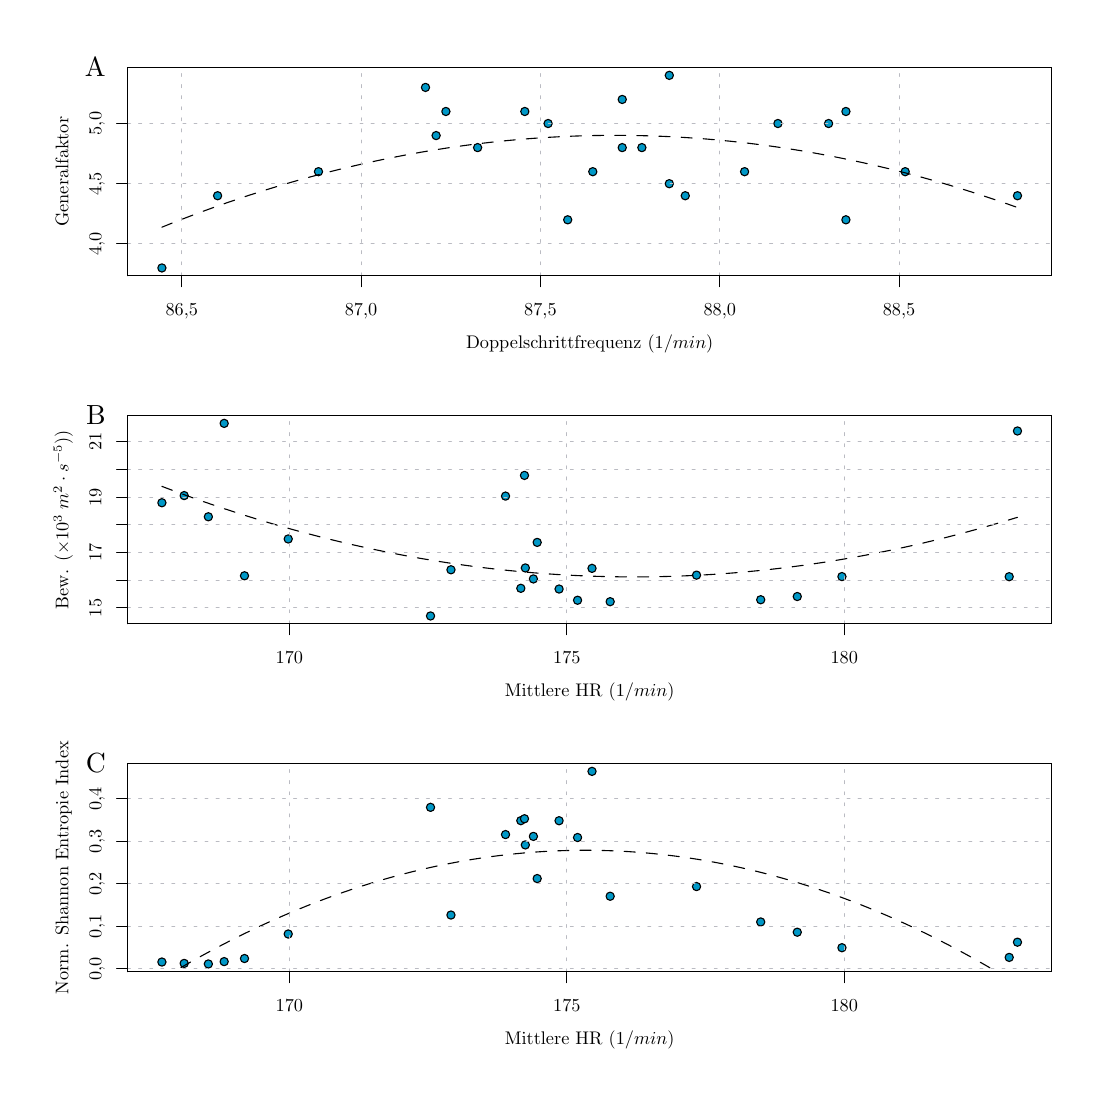
\begin{tikzpicture}[x=1pt,y=1pt]
\definecolor{fillColor}{RGB}{255,255,255}
\path[use as bounding box,fill=fillColor,fill opacity=0.00] (0,0) rectangle (377.25,377.25);
\begin{scope}
\path[clip] ( 36.13,287.63) rectangle (370.02,362.80);
\definecolor{drawColor}{RGB}{0,0,0}
\definecolor{fillColor}{RGB}{0,152,199}

\path[draw=drawColor,line width= 0.4pt,line join=round,line cap=round,fill=fillColor] (259.06,325.21) circle (  1.49);

\path[draw=drawColor,line width= 0.4pt,line join=round,line cap=round,fill=fillColor] (317.09,325.21) circle (  1.49);

\path[draw=drawColor,line width= 0.4pt,line join=round,line cap=round,fill=fillColor] (105.08,325.21) circle (  1.49);

\path[draw=drawColor,line width= 0.4pt,line join=round,line cap=round,fill=fillColor] (231.85,320.87) circle (  1.49);

\path[draw=drawColor,line width= 0.4pt,line join=round,line cap=round,fill=fillColor] (295.66,307.82) circle (  1.49);

\path[draw=drawColor,line width= 0.4pt,line join=round,line cap=round,fill=fillColor] (221.94,333.91) circle (  1.49);

\path[draw=drawColor,line width= 0.4pt,line join=round,line cap=round,fill=fillColor] (162.59,333.91) circle (  1.49);

\path[draw=drawColor,line width= 0.4pt,line join=round,line cap=round,fill=fillColor] (204.20,325.21) circle (  1.49);

\path[draw=drawColor,line width= 0.4pt,line join=round,line cap=round,fill=fillColor] (237.62,316.52) circle (  1.49);

\path[draw=drawColor,line width= 0.4pt,line join=round,line cap=round,fill=fillColor] (195.14,307.82) circle (  1.49);

\path[draw=drawColor,line width= 0.4pt,line join=round,line cap=round,fill=fillColor] ( 48.50,290.42) circle (  1.49);

\path[draw=drawColor,line width= 0.4pt,line join=round,line cap=round,fill=fillColor] ( 68.63,316.52) circle (  1.49);

\path[draw=drawColor,line width= 0.4pt,line join=round,line cap=round,fill=fillColor] (289.41,342.61) circle (  1.49);

\path[draw=drawColor,line width= 0.4pt,line join=round,line cap=round,fill=fillColor] (214.84,333.91) circle (  1.49);

\path[draw=drawColor,line width= 0.4pt,line join=round,line cap=round,fill=fillColor] (214.84,351.31) circle (  1.49);

\path[draw=drawColor,line width= 0.4pt,line join=round,line cap=round,fill=fillColor] (271.10,342.61) circle (  1.49);

\path[draw=drawColor,line width= 0.4pt,line join=round,line cap=round,fill=fillColor] (295.67,346.96) circle (  1.49);

\path[draw=drawColor,line width= 0.4pt,line join=round,line cap=round,fill=fillColor] (147.59,338.26) circle (  1.49);

\path[draw=drawColor,line width= 0.4pt,line join=round,line cap=round,fill=fillColor] (151.12,346.96) circle (  1.49);

\path[draw=drawColor,line width= 0.4pt,line join=round,line cap=round,fill=fillColor] (143.75,355.66) circle (  1.49);

\path[draw=drawColor,line width= 0.4pt,line join=round,line cap=round,fill=fillColor] (231.85,360.01) circle (  1.49);

\path[draw=drawColor,line width= 0.4pt,line join=round,line cap=round,fill=fillColor] (179.64,346.96) circle (  1.49);

\path[draw=drawColor,line width= 0.4pt,line join=round,line cap=round,fill=fillColor] (188.05,342.61) circle (  1.49);

\path[draw=drawColor,line width= 0.4pt,line join=round,line cap=round,fill=fillColor] (357.66,316.52) circle (  1.49);
\end{scope}
\begin{scope}
\path[clip] (  0.00,  0.00) rectangle (377.25,377.25);
\definecolor{drawColor}{RGB}{0,0,0}

\path[draw=drawColor,line width= 0.4pt,line join=round,line cap=round] ( 55.67,287.63) -- (314.89,287.63);

\path[draw=drawColor,line width= 0.4pt,line join=round,line cap=round] ( 55.67,287.63) -- ( 55.67,283.67);

\path[draw=drawColor,line width= 0.4pt,line join=round,line cap=round] (120.48,287.63) -- (120.48,283.67);

\path[draw=drawColor,line width= 0.4pt,line join=round,line cap=round] (185.28,287.63) -- (185.28,283.67);

\path[draw=drawColor,line width= 0.4pt,line join=round,line cap=round] (250.09,287.63) -- (250.09,283.67);

\path[draw=drawColor,line width= 0.4pt,line join=round,line cap=round] (314.89,287.63) -- (314.89,283.67);

\node[text=drawColor,anchor=base,inner sep=0pt, outer sep=0pt, scale=  0.66] at ( 55.67,273.38) {86,5};

\node[text=drawColor,anchor=base,inner sep=0pt, outer sep=0pt, scale=  0.66] at (120.48,273.38) {87,0};

\node[text=drawColor,anchor=base,inner sep=0pt, outer sep=0pt, scale=  0.66] at (185.28,273.38) {87,5};

\node[text=drawColor,anchor=base,inner sep=0pt, outer sep=0pt, scale=  0.66] at (250.09,273.38) {88,0};

\node[text=drawColor,anchor=base,inner sep=0pt, outer sep=0pt, scale=  0.66] at (314.89,273.38) {88,5};

\path[draw=drawColor,line width= 0.4pt,line join=round,line cap=round] ( 36.13,299.12) -- ( 36.13,342.61);

\path[draw=drawColor,line width= 0.4pt,line join=round,line cap=round] ( 36.13,299.12) -- ( 32.17,299.12);

\path[draw=drawColor,line width= 0.4pt,line join=round,line cap=round] ( 36.13,320.87) -- ( 32.17,320.87);

\path[draw=drawColor,line width= 0.4pt,line join=round,line cap=round] ( 36.13,342.61) -- ( 32.17,342.61);

\node[text=drawColor,rotate= 90.00,anchor=base,inner sep=0pt, outer sep=0pt, scale=  0.66] at ( 26.63,299.12) {4,0};

\node[text=drawColor,rotate= 90.00,anchor=base,inner sep=0pt, outer sep=0pt, scale=  0.66] at ( 26.63,320.87) {4,5};

\node[text=drawColor,rotate= 90.00,anchor=base,inner sep=0pt, outer sep=0pt, scale=  0.66] at ( 26.63,342.61) {5,0};

\path[draw=drawColor,line width= 0.4pt,line join=round,line cap=round] ( 36.13,287.63) --
	(370.02,287.63) --
	(370.02,362.80) --
	( 36.13,362.80) --
	( 36.13,287.63);
\end{scope}
\begin{scope}
\path[clip] (  0.00,251.50) rectangle (377.25,377.25);
\definecolor{drawColor}{RGB}{0,0,0}

\node[text=drawColor,anchor=base,inner sep=0pt, outer sep=0pt, scale=  0.66] at (203.08,261.50) {Doppelschrittfrequenz ($1/min$)};

\node[text=drawColor,rotate= 90.00,anchor=base,inner sep=0pt, outer sep=0pt, scale=  0.66] at ( 14.75,325.21) {Generalfaktor};
\end{scope}
\begin{scope}
\path[clip] ( 36.13,287.63) rectangle (370.02,362.80);
\definecolor{drawColor}{RGB}{0,0,0}

\path[draw=drawColor,line width= 0.4pt,dash pattern=on 4pt off 4pt ,line join=round,line cap=round] ( 48.50,305.15) --
	( 51.62,306.40) --
	( 54.75,307.63) --
	( 57.87,308.83) --
	( 60.99,310.01) --
	( 64.12,311.17) --
	( 67.24,312.30) --
	( 70.36,313.41) --
	( 73.48,314.49) --
	( 76.61,315.55) --
	( 79.73,316.59) --
	( 82.85,317.60) --
	( 85.97,318.59) --
	( 89.10,319.55) --
	( 92.22,320.49) --
	( 95.34,321.41) --
	( 98.47,322.30) --
	(101.59,323.17) --
	(104.71,324.01) --
	(107.83,324.83) --
	(110.96,325.62) --
	(114.08,326.40) --
	(117.20,327.14) --
	(120.33,327.87) --
	(123.45,328.56) --
	(126.57,329.24) --
	(129.69,329.89) --
	(132.82,330.51) --
	(135.94,331.12) --
	(139.06,331.69) --
	(142.18,332.25) --
	(145.31,332.78) --
	(148.43,333.28) --
	(151.55,333.77) --
	(154.68,334.22) --
	(157.80,334.66) --
	(160.92,335.07) --
	(164.04,335.45) --
	(167.17,335.81) --
	(170.29,336.15) --
	(173.41,336.46) --
	(176.54,336.75) --
	(179.66,337.02) --
	(182.78,337.26) --
	(185.90,337.47) --
	(189.03,337.67) --
	(192.15,337.83) --
	(195.27,337.98) --
	(198.39,338.10) --
	(201.52,338.19) --
	(204.64,338.27) --
	(207.76,338.31) --
	(210.89,338.34) --
	(214.01,338.34) --
	(217.13,338.31) --
	(220.25,338.26) --
	(223.38,338.19) --
	(226.50,338.09) --
	(229.62,337.97) --
	(232.75,337.83) --
	(235.87,337.66) --
	(238.99,337.46) --
	(242.11,337.25) --
	(245.24,337.01) --
	(248.36,336.74) --
	(251.48,336.45) --
	(254.60,336.14) --
	(257.73,335.80) --
	(260.85,335.44) --
	(263.97,335.05) --
	(267.10,334.64) --
	(270.22,334.21) --
	(273.34,333.75) --
	(276.46,333.26) --
	(279.59,332.76) --
	(282.71,332.23) --
	(285.83,331.67) --
	(288.96,331.09) --
	(292.08,330.49) --
	(295.20,329.86) --
	(298.32,329.21) --
	(301.45,328.54) --
	(304.57,327.84) --
	(307.69,327.11) --
	(310.81,326.37) --
	(313.94,325.59) --
	(317.06,324.80) --
	(320.18,323.98) --
	(323.31,323.13) --
	(326.43,322.26) --
	(329.55,321.37) --
	(332.67,320.46) --
	(335.80,319.52) --
	(338.92,318.55) --
	(342.04,317.56) --
	(345.17,316.55) --
	(348.29,315.51) --
	(351.41,314.45) --
	(354.53,313.37) --
	(357.66,312.26);
\definecolor{drawColor}{RGB}{186,187,194}

\path[draw=drawColor,line width= 0.4pt,dash pattern=on 1pt off 3pt ,line join=round,line cap=round] ( 55.67,287.63) -- ( 55.67,362.80);

\path[draw=drawColor,line width= 0.4pt,dash pattern=on 1pt off 3pt ,line join=round,line cap=round] (120.48,287.63) -- (120.48,362.80);

\path[draw=drawColor,line width= 0.4pt,dash pattern=on 1pt off 3pt ,line join=round,line cap=round] (185.28,287.63) -- (185.28,362.80);

\path[draw=drawColor,line width= 0.4pt,dash pattern=on 1pt off 3pt ,line join=round,line cap=round] (250.09,287.63) -- (250.09,362.80);

\path[draw=drawColor,line width= 0.4pt,dash pattern=on 1pt off 3pt ,line join=round,line cap=round] (314.89,287.63) -- (314.89,362.80);

\path[draw=drawColor,line width= 0.4pt,dash pattern=on 1pt off 3pt ,line join=round,line cap=round] ( 36.14,299.12) -- (370.02,299.12);

\path[draw=drawColor,line width= 0.4pt,dash pattern=on 1pt off 3pt ,line join=round,line cap=round] ( 36.14,320.87) -- (370.02,320.87);

\path[draw=drawColor,line width= 0.4pt,dash pattern=on 1pt off 3pt ,line join=round,line cap=round] ( 36.14,342.61) -- (370.02,342.61);
\end{scope}
\begin{scope}
\path[clip] (  0.00,  0.00) rectangle (377.25,377.25);
\definecolor{drawColor}{RGB}{0,0,0}

\path[draw=drawColor,line width= 0.4pt,line join=round,line cap=round] ( 36.13,287.63) --
	(370.02,287.63) --
	(370.02,362.80) --
	( 36.13,362.80) --
	( 36.13,287.63);

\node[text=drawColor,anchor=base east,inner sep=0pt, outer sep=0pt, scale=  1.00] at ( 28.21,359.65) {A};
\end{scope}
\begin{scope}
\path[clip] ( 36.13,161.88) rectangle (370.02,237.05);
\definecolor{drawColor}{RGB}{0,0,0}
\definecolor{fillColor}{RGB}{0,152,199}

\path[draw=drawColor,line width= 0.4pt,line join=round,line cap=round,fill=fillColor] ( 48.50,205.58) circle (  1.49);

\path[draw=drawColor,line width= 0.4pt,line join=round,line cap=round,fill=fillColor] ( 65.29,200.51) circle (  1.49);

\path[draw=drawColor,line width= 0.4pt,line join=round,line cap=round,fill=fillColor] ( 94.15,192.49) circle (  1.49);

\path[draw=drawColor,line width= 0.4pt,line join=round,line cap=round,fill=fillColor] ( 56.55,208.17) circle (  1.49);

\path[draw=drawColor,line width= 0.4pt,line join=round,line cap=round,fill=fillColor] (184.11,191.25) circle (  1.49);

\path[draw=drawColor,line width= 0.4pt,line join=round,line cap=round,fill=fillColor] (203.92,181.87) circle (  1.49);

\path[draw=drawColor,line width= 0.4pt,line join=round,line cap=round,fill=fillColor] (241.69,179.42) circle (  1.49);

\path[draw=drawColor,line width= 0.4pt,line join=round,line cap=round,fill=fillColor] (182.74,178.05) circle (  1.49);

\path[draw=drawColor,line width= 0.4pt,line join=round,line cap=round,fill=fillColor] (179.83,182.02) circle (  1.49);

\path[draw=drawColor,line width= 0.4pt,line join=round,line cap=round,fill=fillColor] (178.20,174.66) circle (  1.49);

\path[draw=drawColor,line width= 0.4pt,line join=round,line cap=round,fill=fillColor] (145.57,164.67) circle (  1.49);

\path[draw=drawColor,line width= 0.4pt,line join=round,line cap=round,fill=fillColor] (210.48,169.83) circle (  1.49);

\path[draw=drawColor,line width= 0.4pt,line join=round,line cap=round,fill=fillColor] (152.95,181.36) circle (  1.49);

\path[draw=drawColor,line width= 0.4pt,line join=round,line cap=round,fill=fillColor] (198.70,170.35) circle (  1.49);

\path[draw=drawColor,line width= 0.4pt,line join=round,line cap=round,fill=fillColor] (264.88,170.53) circle (  1.49);

\path[draw=drawColor,line width= 0.4pt,line join=round,line cap=round,fill=fillColor] (354.67,178.86) circle (  1.49);

\path[draw=drawColor,line width= 0.4pt,line join=round,line cap=round,fill=fillColor] ( 78.35,179.19) circle (  1.49);

\path[draw=drawColor,line width= 0.4pt,line join=round,line cap=round,fill=fillColor] (192.02,174.40) circle (  1.49);

\path[draw=drawColor,line width= 0.4pt,line join=round,line cap=round,fill=fillColor] (278.09,171.69) circle (  1.49);

\path[draw=drawColor,line width= 0.4pt,line join=round,line cap=round,fill=fillColor] (294.23,178.90) circle (  1.49);

\path[draw=drawColor,line width= 0.4pt,line join=round,line cap=round,fill=fillColor] ( 71.00,234.26) circle (  1.49);

\path[draw=drawColor,line width= 0.4pt,line join=round,line cap=round,fill=fillColor] (179.52,215.46) circle (  1.49);

\path[draw=drawColor,line width= 0.4pt,line join=round,line cap=round,fill=fillColor] (172.67,207.98) circle (  1.49);

\path[draw=drawColor,line width= 0.4pt,line join=round,line cap=round,fill=fillColor] (357.66,231.51) circle (  1.49);
\end{scope}
\begin{scope}
\path[clip] (  0.00,  0.00) rectangle (377.25,377.25);
\definecolor{drawColor}{RGB}{0,0,0}

\path[draw=drawColor,line width= 0.4pt,line join=round,line cap=round] ( 94.56,161.88) -- (295.07,161.88);

\path[draw=drawColor,line width= 0.4pt,line join=round,line cap=round] ( 94.56,161.88) -- ( 94.56,157.92);

\path[draw=drawColor,line width= 0.4pt,line join=round,line cap=round] (194.82,161.88) -- (194.82,157.92);

\path[draw=drawColor,line width= 0.4pt,line join=round,line cap=round] (295.07,161.88) -- (295.07,157.92);

\node[text=drawColor,anchor=base,inner sep=0pt, outer sep=0pt, scale=  0.66] at ( 94.56,147.63) {170};

\node[text=drawColor,anchor=base,inner sep=0pt, outer sep=0pt, scale=  0.66] at (194.82,147.63) {175};

\node[text=drawColor,anchor=base,inner sep=0pt, outer sep=0pt, scale=  0.66] at (295.07,147.63) {180};

\path[draw=drawColor,line width= 0.4pt,line join=round,line cap=round] ( 36.13,167.57) -- ( 36.13,227.66);

\path[draw=drawColor,line width= 0.4pt,line join=round,line cap=round] ( 36.13,167.57) -- ( 32.17,167.57);

\path[draw=drawColor,line width= 0.4pt,line join=round,line cap=round] ( 36.13,177.58) -- ( 32.17,177.58);

\path[draw=drawColor,line width= 0.4pt,line join=round,line cap=round] ( 36.13,187.60) -- ( 32.17,187.60);

\path[draw=drawColor,line width= 0.4pt,line join=round,line cap=round] ( 36.13,197.61) -- ( 32.17,197.61);

\path[draw=drawColor,line width= 0.4pt,line join=round,line cap=round] ( 36.13,207.63) -- ( 32.17,207.63);

\path[draw=drawColor,line width= 0.4pt,line join=round,line cap=round] ( 36.13,217.65) -- ( 32.17,217.65);

\path[draw=drawColor,line width= 0.4pt,line join=round,line cap=round] ( 36.13,227.66) -- ( 32.17,227.66);

\node[text=drawColor,rotate= 90.00,anchor=base,inner sep=0pt, outer sep=0pt, scale=  0.66] at ( 26.63,167.57) {15};

\node[text=drawColor,rotate= 90.00,anchor=base,inner sep=0pt, outer sep=0pt, scale=  0.66] at ( 26.63,187.60) {17};

\node[text=drawColor,rotate= 90.00,anchor=base,inner sep=0pt, outer sep=0pt, scale=  0.66] at ( 26.63,207.63) {19};

\node[text=drawColor,rotate= 90.00,anchor=base,inner sep=0pt, outer sep=0pt, scale=  0.66] at ( 26.63,227.66) {21};

\path[draw=drawColor,line width= 0.4pt,line join=round,line cap=round] ( 36.13,161.88) --
	(370.02,161.88) --
	(370.02,237.05) --
	( 36.13,237.05) --
	( 36.13,161.88);
\end{scope}
\begin{scope}
\path[clip] (  0.00,125.75) rectangle (377.25,251.50);
\definecolor{drawColor}{RGB}{0,0,0}

\node[text=drawColor,anchor=base,inner sep=0pt, outer sep=0pt, scale=  0.66] at (203.08,135.75) {Mittlere HR ($1/min$)};

\node[text=drawColor,rotate= 90.00,anchor=base,inner sep=0pt, outer sep=0pt, scale=  0.66] at ( 14.75,199.47) {Bew. ($\times 10^3 \: m^2 \cdot s^{-5}$))};
\end{scope}
\begin{scope}
\path[clip] ( 36.13,161.88) rectangle (370.02,237.05);
\definecolor{drawColor}{RGB}{0,0,0}

\path[draw=drawColor,line width= 0.4pt,dash pattern=on 4pt off 4pt ,line join=round,line cap=round] ( 48.50,211.50) --
	( 51.62,210.32) --
	( 54.75,209.15) --
	( 57.87,208.01) --
	( 60.99,206.89) --
	( 64.12,205.79) --
	( 67.24,204.72) --
	( 70.36,203.66) --
	( 73.48,202.63) --
	( 76.61,201.62) --
	( 79.73,200.63) --
	( 82.85,199.66) --
	( 85.97,198.71) --
	( 89.10,197.79) --
	( 92.22,196.89) --
	( 95.34,196.01) --
	( 98.47,195.15) --
	(101.59,194.32) --
	(104.71,193.50) --
	(107.83,192.71) --
	(110.96,191.94) --
	(114.08,191.19) --
	(117.20,190.46) --
	(120.33,189.76) --
	(123.45,189.08) --
	(126.57,188.42) --
	(129.69,187.78) --
	(132.82,187.16) --
	(135.94,186.57) --
	(139.06,185.99) --
	(142.18,185.44) --
	(145.31,184.91) --
	(148.43,184.41) --
	(151.55,183.92) --
	(154.68,183.46) --
	(157.80,183.02) --
	(160.92,182.60) --
	(164.04,182.20) --
	(167.17,181.82) --
	(170.29,181.47) --
	(173.41,181.14) --
	(176.54,180.83) --
	(179.66,180.54) --
	(182.78,180.27) --
	(185.90,180.03) --
	(189.03,179.81) --
	(192.15,179.60) --
	(195.27,179.43) --
	(198.39,179.27) --
	(201.52,179.13) --
	(204.64,179.02) --
	(207.76,178.93) --
	(210.89,178.86) --
	(214.01,178.81) --
	(217.13,178.79) --
	(220.25,178.79) --
	(223.38,178.80) --
	(226.50,178.84) --
	(229.62,178.91) --
	(232.75,178.99) --
	(235.87,179.10) --
	(238.99,179.23) --
	(242.11,179.38) --
	(245.24,179.55) --
	(248.36,179.74) --
	(251.48,179.96) --
	(254.60,180.19) --
	(257.73,180.45) --
	(260.85,180.74) --
	(263.97,181.04) --
	(267.10,181.36) --
	(270.22,181.71) --
	(273.34,182.08) --
	(276.46,182.47) --
	(279.59,182.88) --
	(282.71,183.32) --
	(285.83,183.78) --
	(288.96,184.25) --
	(292.08,184.75) --
	(295.20,185.28) --
	(298.32,185.82) --
	(301.45,186.39) --
	(304.57,186.98) --
	(307.69,187.59) --
	(310.81,188.22) --
	(313.94,188.87) --
	(317.06,189.55) --
	(320.18,190.24) --
	(323.31,190.96) --
	(326.43,191.71) --
	(329.55,192.47) --
	(332.67,193.25) --
	(335.80,194.06) --
	(338.92,194.89) --
	(342.04,195.74) --
	(345.17,196.61) --
	(348.29,197.51) --
	(351.41,198.43) --
	(354.53,199.36) --
	(357.66,200.32);
\definecolor{drawColor}{RGB}{186,187,194}

\path[draw=drawColor,line width= 0.4pt,dash pattern=on 1pt off 3pt ,line join=round,line cap=round] ( 94.56,161.88) -- ( 94.56,237.05);

\path[draw=drawColor,line width= 0.4pt,dash pattern=on 1pt off 3pt ,line join=round,line cap=round] (194.82,161.88) -- (194.82,237.05);

\path[draw=drawColor,line width= 0.4pt,dash pattern=on 1pt off 3pt ,line join=round,line cap=round] (295.07,161.88) -- (295.07,237.05);

\path[draw=drawColor,line width= 0.4pt,dash pattern=on 1pt off 3pt ,line join=round,line cap=round] ( 36.13,167.57) -- (370.02,167.57);

\path[draw=drawColor,line width= 0.4pt,dash pattern=on 1pt off 3pt ,line join=round,line cap=round] ( 36.13,177.58) -- (370.02,177.58);

\path[draw=drawColor,line width= 0.4pt,dash pattern=on 1pt off 3pt ,line join=round,line cap=round] ( 36.13,187.60) -- (370.02,187.60);

\path[draw=drawColor,line width= 0.4pt,dash pattern=on 1pt off 3pt ,line join=round,line cap=round] ( 36.13,197.61) -- (370.02,197.61);

\path[draw=drawColor,line width= 0.4pt,dash pattern=on 1pt off 3pt ,line join=round,line cap=round] ( 36.13,207.63) -- (370.02,207.63);

\path[draw=drawColor,line width= 0.4pt,dash pattern=on 1pt off 3pt ,line join=round,line cap=round] ( 36.13,217.65) -- (370.02,217.65);

\path[draw=drawColor,line width= 0.4pt,dash pattern=on 1pt off 3pt ,line join=round,line cap=round] ( 36.13,227.66) -- (370.02,227.66);
\end{scope}
\begin{scope}
\path[clip] (  0.00,  0.00) rectangle (377.25,377.25);
\definecolor{drawColor}{RGB}{0,0,0}

\path[draw=drawColor,line width= 0.4pt,line join=round,line cap=round] ( 36.13,161.88) --
	(370.02,161.88) --
	(370.02,237.05) --
	( 36.13,237.05) --
	( 36.13,161.88);

\node[text=drawColor,anchor=base east,inner sep=0pt, outer sep=0pt, scale=  1.00] at ( 28.21,233.90) {B};
\end{scope}
\begin{scope}
\path[clip] ( 36.13, 36.13) rectangle (370.02,111.30);
\definecolor{drawColor}{RGB}{0,0,0}
\definecolor{fillColor}{RGB}{0,152,199}

\path[draw=drawColor,line width= 0.4pt,line join=round,line cap=round,fill=fillColor] ( 48.50, 39.62) circle (  1.49);

\path[draw=drawColor,line width= 0.4pt,line join=round,line cap=round,fill=fillColor] ( 65.29, 38.92) circle (  1.49);

\path[draw=drawColor,line width= 0.4pt,line join=round,line cap=round,fill=fillColor] ( 94.15, 49.75) circle (  1.49);

\path[draw=drawColor,line width= 0.4pt,line join=round,line cap=round,fill=fillColor] ( 56.55, 39.13) circle (  1.49);

\path[draw=drawColor,line width= 0.4pt,line join=round,line cap=round,fill=fillColor] (184.11, 69.78) circle (  1.49);

\path[draw=drawColor,line width= 0.4pt,line join=round,line cap=round,fill=fillColor] (203.92,108.51) circle (  1.49);

\path[draw=drawColor,line width= 0.4pt,line join=round,line cap=round,fill=fillColor] (241.69, 66.89) circle (  1.49);

\path[draw=drawColor,line width= 0.4pt,line join=round,line cap=round,fill=fillColor] (182.74, 85.02) circle (  1.49);

\path[draw=drawColor,line width= 0.4pt,line join=round,line cap=round,fill=fillColor] (179.83, 81.94) circle (  1.49);

\path[draw=drawColor,line width= 0.4pt,line join=round,line cap=round,fill=fillColor] (178.20, 90.70) circle (  1.49);

\path[draw=drawColor,line width= 0.4pt,line join=round,line cap=round,fill=fillColor] (145.57, 95.52) circle (  1.49);

\path[draw=drawColor,line width= 0.4pt,line join=round,line cap=round,fill=fillColor] (210.48, 63.39) circle (  1.49);

\path[draw=drawColor,line width= 0.4pt,line join=round,line cap=round,fill=fillColor] (152.95, 56.60) circle (  1.49);

\path[draw=drawColor,line width= 0.4pt,line join=round,line cap=round,fill=fillColor] (198.70, 84.61) circle (  1.49);

\path[draw=drawColor,line width= 0.4pt,line join=round,line cap=round,fill=fillColor] (264.88, 54.10) circle (  1.49);

\path[draw=drawColor,line width= 0.4pt,line join=round,line cap=round,fill=fillColor] (354.67, 41.29) circle (  1.49);

\path[draw=drawColor,line width= 0.4pt,line join=round,line cap=round,fill=fillColor] ( 78.35, 40.89) circle (  1.49);

\path[draw=drawColor,line width= 0.4pt,line join=round,line cap=round,fill=fillColor] (192.02, 90.68) circle (  1.49);

\path[draw=drawColor,line width= 0.4pt,line join=round,line cap=round,fill=fillColor] (278.09, 50.40) circle (  1.49);

\path[draw=drawColor,line width= 0.4pt,line join=round,line cap=round,fill=fillColor] (294.23, 44.79) circle (  1.49);

\path[draw=drawColor,line width= 0.4pt,line join=round,line cap=round,fill=fillColor] ( 71.00, 39.77) circle (  1.49);

\path[draw=drawColor,line width= 0.4pt,line join=round,line cap=round,fill=fillColor] (179.52, 91.39) circle (  1.49);

\path[draw=drawColor,line width= 0.4pt,line join=round,line cap=round,fill=fillColor] (172.67, 85.68) circle (  1.49);

\path[draw=drawColor,line width= 0.4pt,line join=round,line cap=round,fill=fillColor] (357.66, 46.79) circle (  1.49);
\end{scope}
\begin{scope}
\path[clip] (  0.00,  0.00) rectangle (377.25,377.25);
\definecolor{drawColor}{RGB}{0,0,0}

\path[draw=drawColor,line width= 0.4pt,line join=round,line cap=round] ( 94.56, 36.13) -- (295.07, 36.13);

\path[draw=drawColor,line width= 0.4pt,line join=round,line cap=round] ( 94.56, 36.13) -- ( 94.56, 32.17);

\path[draw=drawColor,line width= 0.4pt,line join=round,line cap=round] (194.82, 36.13) -- (194.82, 32.17);

\path[draw=drawColor,line width= 0.4pt,line join=round,line cap=round] (295.07, 36.13) -- (295.07, 32.17);

\node[text=drawColor,anchor=base,inner sep=0pt, outer sep=0pt, scale=  0.66] at ( 94.56, 21.88) {170};

\node[text=drawColor,anchor=base,inner sep=0pt, outer sep=0pt, scale=  0.66] at (194.82, 21.88) {175};

\node[text=drawColor,anchor=base,inner sep=0pt, outer sep=0pt, scale=  0.66] at (295.07, 21.88) {180};

\path[draw=drawColor,line width= 0.4pt,line join=round,line cap=round] ( 36.13, 37.14) -- ( 36.13, 98.58);

\path[draw=drawColor,line width= 0.4pt,line join=round,line cap=round] ( 36.13, 37.14) -- ( 32.17, 37.14);

\path[draw=drawColor,line width= 0.4pt,line join=round,line cap=round] ( 36.13, 52.50) -- ( 32.17, 52.50);

\path[draw=drawColor,line width= 0.4pt,line join=round,line cap=round] ( 36.13, 67.86) -- ( 32.17, 67.86);

\path[draw=drawColor,line width= 0.4pt,line join=round,line cap=round] ( 36.13, 83.22) -- ( 32.17, 83.22);

\path[draw=drawColor,line width= 0.4pt,line join=round,line cap=round] ( 36.13, 98.58) -- ( 32.17, 98.58);

\node[text=drawColor,rotate= 90.00,anchor=base,inner sep=0pt, outer sep=0pt, scale=  0.66] at ( 26.63, 37.14) {0,0};

\node[text=drawColor,rotate= 90.00,anchor=base,inner sep=0pt, outer sep=0pt, scale=  0.66] at ( 26.63, 52.50) {0,1};

\node[text=drawColor,rotate= 90.00,anchor=base,inner sep=0pt, outer sep=0pt, scale=  0.66] at ( 26.63, 67.86) {0,2};

\node[text=drawColor,rotate= 90.00,anchor=base,inner sep=0pt, outer sep=0pt, scale=  0.66] at ( 26.63, 83.22) {0,3};

\node[text=drawColor,rotate= 90.00,anchor=base,inner sep=0pt, outer sep=0pt, scale=  0.66] at ( 26.63, 98.58) {0,4};

\path[draw=drawColor,line width= 0.4pt,line join=round,line cap=round] ( 36.13, 36.13) --
	(370.02, 36.13) --
	(370.02,111.30) --
	( 36.13,111.30) --
	( 36.13, 36.13);
\end{scope}
\begin{scope}
\path[clip] (  0.00,  0.00) rectangle (377.25,125.75);
\definecolor{drawColor}{RGB}{0,0,0}

\node[text=drawColor,anchor=base,inner sep=0pt, outer sep=0pt, scale=  0.66] at (203.08, 10.00) {Mittlere HR ($1/min$)};

\node[text=drawColor,rotate= 90.00,anchor=base,inner sep=0pt, outer sep=0pt, scale=  0.66] at ( 14.75, 73.72) {Norm. Shannon Entropie Index};
\end{scope}
\begin{scope}
\path[clip] ( 36.13, 36.13) rectangle (370.02,111.30);
\definecolor{drawColor}{RGB}{0,0,0}

\path[draw=drawColor,line width= 0.4pt,dash pattern=on 4pt off 4pt ,line join=round,line cap=round] ( 48.50, 33.53) --
	( 51.62, 35.41) --
	( 54.75, 37.24) --
	( 57.87, 39.05) --
	( 60.99, 40.81) --
	( 64.12, 42.53) --
	( 67.24, 44.22) --
	( 70.36, 45.86) --
	( 73.48, 47.47) --
	( 76.61, 49.04) --
	( 79.73, 50.57) --
	( 82.85, 52.06) --
	( 85.97, 53.51) --
	( 89.10, 54.92) --
	( 92.22, 56.30) --
	( 95.34, 57.63) --
	( 98.47, 58.93) --
	(101.59, 60.19) --
	(104.71, 61.41) --
	(107.83, 62.59) --
	(110.96, 63.73) --
	(114.08, 64.83) --
	(117.20, 65.90) --
	(120.33, 66.93) --
	(123.45, 67.91) --
	(126.57, 68.86) --
	(129.69, 69.77) --
	(132.82, 70.64) --
	(135.94, 71.47) --
	(139.06, 72.27) --
	(142.18, 73.02) --
	(145.31, 73.74) --
	(148.43, 74.42) --
	(151.55, 75.05) --
	(154.68, 75.65) --
	(157.80, 76.22) --
	(160.92, 76.74) --
	(164.04, 77.22) --
	(167.17, 77.67) --
	(170.29, 78.07) --
	(173.41, 78.44) --
	(176.54, 78.77) --
	(179.66, 79.06) --
	(182.78, 79.31) --
	(185.90, 79.52) --
	(189.03, 79.70) --
	(192.15, 79.83) --
	(195.27, 79.93) --
	(198.39, 79.99) --
	(201.52, 80.01) --
	(204.64, 79.99) --
	(207.76, 79.93) --
	(210.89, 79.83) --
	(214.01, 79.69) --
	(217.13, 79.52) --
	(220.25, 79.31) --
	(223.38, 79.05) --
	(226.50, 78.76) --
	(229.62, 78.43) --
	(232.75, 78.06) --
	(235.87, 77.66) --
	(238.99, 77.21) --
	(242.11, 76.73) --
	(245.24, 76.20) --
	(248.36, 75.64) --
	(251.48, 75.04) --
	(254.60, 74.40) --
	(257.73, 73.72) --
	(260.85, 73.01) --
	(263.97, 72.25) --
	(267.10, 71.46) --
	(270.22, 70.62) --
	(273.34, 69.75) --
	(276.46, 68.84) --
	(279.59, 67.89) --
	(282.71, 66.90) --
	(285.83, 65.87) --
	(288.96, 64.81) --
	(292.08, 63.70) --
	(295.20, 62.56) --
	(298.32, 61.38) --
	(301.45, 60.16) --
	(304.57, 58.90) --
	(307.69, 57.60) --
	(310.81, 56.27) --
	(313.94, 54.89) --
	(317.06, 53.48) --
	(320.18, 52.02) --
	(323.31, 50.53) --
	(326.43, 49.00) --
	(329.55, 47.43) --
	(332.67, 45.82) --
	(335.80, 44.18) --
	(338.92, 42.49) --
	(342.04, 40.77) --
	(345.17, 39.00) --
	(348.29, 37.20) --
	(351.41, 35.36) --
	(354.53, 33.48) --
	(357.66, 31.57);
\definecolor{drawColor}{RGB}{186,187,194}

\path[draw=drawColor,line width= 0.4pt,dash pattern=on 1pt off 3pt ,line join=round,line cap=round] ( 94.56, 36.13) -- ( 94.56,111.30);

\path[draw=drawColor,line width= 0.4pt,dash pattern=on 1pt off 3pt ,line join=round,line cap=round] (194.82, 36.13) -- (194.82,111.30);

\path[draw=drawColor,line width= 0.4pt,dash pattern=on 1pt off 3pt ,line join=round,line cap=round] (295.07, 36.13) -- (295.07,111.30);

\path[draw=drawColor,line width= 0.4pt,dash pattern=on 1pt off 3pt ,line join=round,line cap=round] ( 36.13, 37.14) -- (370.02, 37.14);

\path[draw=drawColor,line width= 0.4pt,dash pattern=on 1pt off 3pt ,line join=round,line cap=round] ( 36.13, 52.50) -- (370.02, 52.50);

\path[draw=drawColor,line width= 0.4pt,dash pattern=on 1pt off 3pt ,line join=round,line cap=round] ( 36.13, 67.86) -- (370.02, 67.86);

\path[draw=drawColor,line width= 0.4pt,dash pattern=on 1pt off 3pt ,line join=round,line cap=round] ( 36.13, 83.22) -- (370.02, 83.22);

\path[draw=drawColor,line width= 0.4pt,dash pattern=on 1pt off 3pt ,line join=round,line cap=round] ( 36.13, 98.58) -- (370.02, 98.58);
\end{scope}
\begin{scope}
\path[clip] (  0.00,  0.00) rectangle (377.25,377.25);
\definecolor{drawColor}{RGB}{0,0,0}

\path[draw=drawColor,line width= 0.4pt,line join=round,line cap=round] ( 36.13, 36.13) --
	(370.02, 36.13) --
	(370.02,111.30) --
	( 36.13,111.30) --
	( 36.13, 36.13);

\node[text=drawColor,anchor=base east,inner sep=0pt, outer sep=0pt, scale=  1.00] at ( 28.21,108.15) {C};
\end{scope}
\end{tikzpicture}
 \caption[Quadratische Zusammenhänge zwischen expliziten und impliziten Merkmalen (Erste Studie: Laufen)]{Quadratische Zusammenhänge zwischen expliziten und impliziten Merkmalen beim Laufen -- (A) Generalfaktor und mittlere Doppelschrittfrequenz; (B) mittlerer Bewegungsaufwand und mittlere \ac{HR}; (C) Mittlerer normalisierter Shannon Entropie Index und mittlere \ac{HR}.\\
	\hspace{ 
	\textwidth}\emph{Anmerkung}: Gestrichelte Linie stellt das bestmögliche quadratische Modell dar.} \label{fig:regressionsanalyse_1} 
\end{figure}

Ich führte Regressionsanalysen durch, um quadratische Zusammenhänge wie z.~B. bei \citet{Peifer2014} zu finden ($y=\beta_{0}+\beta_{1}x+\beta_{2}x^{2}+e$). Dabei testete ich quadratische Ausdrücke auf der Seite der unabhängigen Variable $x$. Zur Bestimmung der Modellparameter $\beta_i$ wird eine lineare Regression mit der Methode der kleinsten Quadrate eingesetzt. 

Ich fand einen signifikanten Zusammenhang zwischen einem expliziten erhobenen Merkmal und einem implizit gemessenen Merkmal. Der Zusammenhang zwischen Flow-Erleben, gemessen durch den Generalfaktor der \ac{FKS}, und der mittleren Doppelschrittfrequenz drückt sich durch ein umgedrehtes U aus, $R^2 = 0{,}3; F(2, 21) = 4{,}41; p < 0{,}05$ (Abbildung~\ref{fig:regressionsanalyse_1},~A). Alle weiteren signifikanten Zusammenhänge bestehen zwischen zwei implizit gemessenen Merkmalen. Die Ergebnisse zeigen einen Zusammenhang in Form eines Us zwischen dem mittleren Bewegungsaufwand und der mittleren \ac{HR}, $R^2 = 0{,}33; F(2, 21) = 5{,}11; p < 0{,}05$ (Abbildung~\ref{fig:regressionsanalyse_1},~B) und einen Zusammenhang in Form eines umgedrehten Us zwischen dem mittleren normalisierten Shannon Entropie Index der kardio-lokomotorischen Phasensynchronisation und der mittleren \ac{HR}, $R^2 = 0{,}64; F(2, 21) = 18{,}85; p < 0{,}001$ (Abbildung~\ref{fig:regressionsanalyse_1},~C).

% subsubsection regressionsanalyse (end)
\subsubsection{Prozessorientierter Ansatz} 

% (fold)
\label{ssub:prozessorientierter_ansatz_5_1} 
\begin{sidewaysfigure}
	\resizebox{1.00 
	\textwidth}{!}{
	
	%
	% Created by tikzDevice version 0.10.1 on 2016-09-06 14:04:50
% !TEX encoding = UTF-8 Unicode
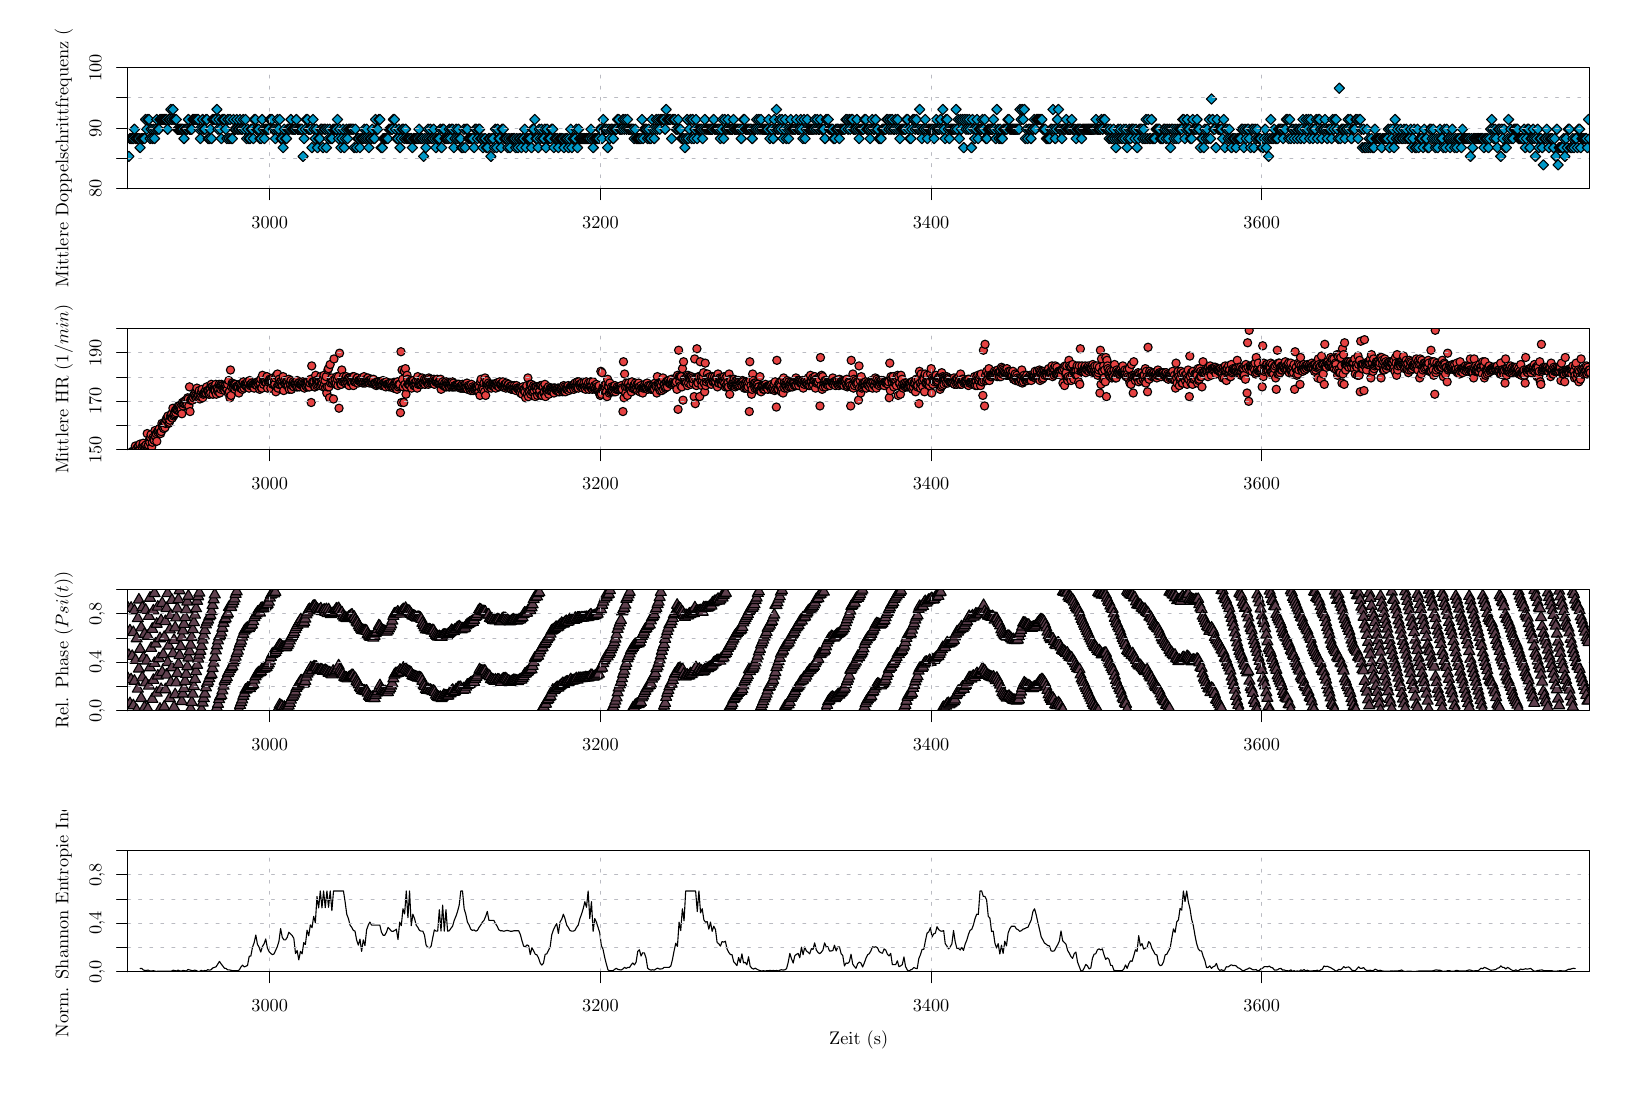
\begin{tikzpicture}[x=1pt,y=1pt]
\definecolor{fillColor}{RGB}{255,255,255}
\path[use as bounding box,fill=fillColor,fill opacity=0.00] (0,0) rectangle (571.66,377.25);
\begin{scope}
\path[clip] ( 36.13,319.07) rectangle (564.43,362.80);
\definecolor{drawColor}{RGB}{0,0,0}
\definecolor{fillColor}{RGB}{0,152,199}

\path[draw=drawColor,line width= 0.4pt,line join=round,line cap=round,fill=fillColor] ( 36.14,142.36) --
	( 38.00,144.22) --
	( 36.14,146.08) --
	( 34.27,144.22) --
	cycle;

\path[draw=drawColor,line width= 0.4pt,line join=round,line cap=round,fill=fillColor] ( 36.56,328.87) --
	( 38.42,330.73) --
	( 36.56,332.59) --
	( 34.69,330.73) --
	cycle;

\path[draw=drawColor,line width= 0.4pt,line join=round,line cap=round,fill=fillColor] ( 36.96,335.30) --
	( 38.82,337.16) --
	( 36.96,339.03) --
	( 35.10,337.16) --
	cycle;

\path[draw=drawColor,line width= 0.4pt,line join=round,line cap=round,fill=fillColor] ( 37.37,335.30) --
	( 39.23,337.16) --
	( 37.37,339.03) --
	( 35.51,337.16) --
	cycle;

\path[draw=drawColor,line width= 0.4pt,line join=round,line cap=round,fill=fillColor] ( 37.77,335.30) --
	( 39.63,337.16) --
	( 37.77,339.03) --
	( 35.91,337.16) --
	cycle;

\path[draw=drawColor,line width= 0.4pt,line join=round,line cap=round,fill=fillColor] ( 38.18,335.30) --
	( 40.04,337.16) --
	( 38.18,339.03) --
	( 36.32,337.16) --
	cycle;

\path[draw=drawColor,line width= 0.4pt,line join=round,line cap=round,fill=fillColor] ( 38.58,338.69) --
	( 40.44,340.55) --
	( 38.58,342.41) --
	( 36.72,340.55) --
	cycle;

\path[draw=drawColor,line width= 0.4pt,line join=round,line cap=round,fill=fillColor] ( 38.98,335.30) --
	( 40.85,337.16) --
	( 38.98,339.03) --
	( 37.12,337.16) --
	cycle;

\path[draw=drawColor,line width= 0.4pt,line join=round,line cap=round,fill=fillColor] ( 39.39,335.30) --
	( 41.25,337.16) --
	( 39.39,339.03) --
	( 37.53,337.16) --
	cycle;

\path[draw=drawColor,line width= 0.4pt,line join=round,line cap=round,fill=fillColor] ( 39.80,335.30) --
	( 41.66,337.16) --
	( 39.80,339.03) --
	( 37.94,337.16) --
	cycle;

\path[draw=drawColor,line width= 0.4pt,line join=round,line cap=round,fill=fillColor] ( 40.20,335.30) --
	( 42.06,337.16) --
	( 40.20,339.03) --
	( 38.34,337.16) --
	cycle;

\path[draw=drawColor,line width= 0.4pt,line join=round,line cap=round,fill=fillColor] ( 40.62,332.03) --
	( 42.48,333.89) --
	( 40.62,335.75) --
	( 38.75,333.89) --
	cycle;

\path[draw=drawColor,line width= 0.4pt,line join=round,line cap=round,fill=fillColor] ( 41.02,335.30) --
	( 42.88,337.16) --
	( 41.02,339.03) --
	( 39.16,337.16) --
	cycle;

\path[draw=drawColor,line width= 0.4pt,line join=round,line cap=round,fill=fillColor] ( 41.43,335.30) --
	( 43.29,337.16) --
	( 41.43,339.03) --
	( 39.57,337.16) --
	cycle;

\path[draw=drawColor,line width= 0.4pt,line join=round,line cap=round,fill=fillColor] ( 41.83,335.30) --
	( 43.70,337.16) --
	( 41.83,339.03) --
	( 39.97,337.16) --
	cycle;

\path[draw=drawColor,line width= 0.4pt,line join=round,line cap=round,fill=fillColor] ( 42.24,335.30) --
	( 44.10,337.16) --
	( 42.24,339.03) --
	( 40.38,337.16) --
	cycle;

\path[draw=drawColor,line width= 0.4pt,line join=round,line cap=round,fill=fillColor] ( 42.63,342.20) --
	( 44.49,344.06) --
	( 42.63,345.92) --
	( 40.77,344.06) --
	cycle;

\path[draw=drawColor,line width= 0.4pt,line join=round,line cap=round,fill=fillColor] ( 43.03,338.69) --
	( 44.89,340.55) --
	( 43.03,342.41) --
	( 41.17,340.55) --
	cycle;

\path[draw=drawColor,line width= 0.4pt,line join=round,line cap=round,fill=fillColor] ( 43.42,342.20) --
	( 45.28,344.06) --
	( 43.42,345.92) --
	( 41.56,344.06) --
	cycle;

\path[draw=drawColor,line width= 0.4pt,line join=round,line cap=round,fill=fillColor] ( 43.82,342.20) --
	( 45.68,344.06) --
	( 43.82,345.92) --
	( 41.95,344.06) --
	cycle;

\path[draw=drawColor,line width= 0.4pt,line join=round,line cap=round,fill=fillColor] ( 44.22,335.30) --
	( 46.08,337.16) --
	( 44.22,339.03) --
	( 42.36,337.16) --
	cycle;

\path[draw=drawColor,line width= 0.4pt,line join=round,line cap=round,fill=fillColor] ( 44.62,338.69) --
	( 46.48,340.55) --
	( 44.62,342.41) --
	( 42.76,340.55) --
	cycle;

\path[draw=drawColor,line width= 0.4pt,line join=round,line cap=round,fill=fillColor] ( 45.03,335.30) --
	( 46.89,337.16) --
	( 45.03,339.03) --
	( 43.17,337.16) --
	cycle;

\path[draw=drawColor,line width= 0.4pt,line join=round,line cap=round,fill=fillColor] ( 45.43,338.69) --
	( 47.29,340.55) --
	( 45.43,342.41) --
	( 43.56,340.55) --
	cycle;

\path[draw=drawColor,line width= 0.4pt,line join=round,line cap=round,fill=fillColor] ( 45.83,335.30) --
	( 47.69,337.16) --
	( 45.83,339.03) --
	( 43.97,337.16) --
	cycle;

\path[draw=drawColor,line width= 0.4pt,line join=round,line cap=round,fill=fillColor] ( 46.23,338.69) --
	( 48.09,340.55) --
	( 46.23,342.41) --
	( 44.37,340.55) --
	cycle;

\path[draw=drawColor,line width= 0.4pt,line join=round,line cap=round,fill=fillColor] ( 46.62,342.20) --
	( 48.48,344.06) --
	( 46.62,345.92) --
	( 44.76,344.06) --
	cycle;

\path[draw=drawColor,line width= 0.4pt,line join=round,line cap=round,fill=fillColor] ( 47.02,338.69) --
	( 48.88,340.55) --
	( 47.02,342.41) --
	( 45.16,340.55) --
	cycle;

\path[draw=drawColor,line width= 0.4pt,line join=round,line cap=round,fill=fillColor] ( 47.42,338.69) --
	( 49.28,340.55) --
	( 47.42,342.41) --
	( 45.56,340.55) --
	cycle;

\path[draw=drawColor,line width= 0.4pt,line join=round,line cap=round,fill=fillColor] ( 47.81,342.20) --
	( 49.67,344.06) --
	( 47.81,345.92) --
	( 45.95,344.06) --
	cycle;

\path[draw=drawColor,line width= 0.4pt,line join=round,line cap=round,fill=fillColor] ( 48.21,342.20) --
	( 50.07,344.06) --
	( 48.21,345.92) --
	( 46.34,344.06) --
	cycle;

\path[draw=drawColor,line width= 0.4pt,line join=round,line cap=round,fill=fillColor] ( 48.60,342.20) --
	( 50.46,344.06) --
	( 48.60,345.92) --
	( 46.74,344.06) --
	cycle;

\path[draw=drawColor,line width= 0.4pt,line join=round,line cap=round,fill=fillColor] ( 48.99,342.20) --
	( 50.85,344.06) --
	( 48.99,345.92) --
	( 47.13,344.06) --
	cycle;

\path[draw=drawColor,line width= 0.4pt,line join=round,line cap=round,fill=fillColor] ( 49.38,342.20) --
	( 51.24,344.06) --
	( 49.38,345.92) --
	( 47.52,344.06) --
	cycle;

\path[draw=drawColor,line width= 0.4pt,line join=round,line cap=round,fill=fillColor] ( 49.77,342.20) --
	( 51.63,344.06) --
	( 49.77,345.92) --
	( 47.91,344.06) --
	cycle;

\path[draw=drawColor,line width= 0.4pt,line join=round,line cap=round,fill=fillColor] ( 50.17,342.20) --
	( 52.03,344.06) --
	( 50.17,345.92) --
	( 48.30,344.06) --
	cycle;

\path[draw=drawColor,line width= 0.4pt,line join=round,line cap=round,fill=fillColor] ( 50.56,338.69) --
	( 52.43,340.55) --
	( 50.56,342.41) --
	( 48.70,340.55) --
	cycle;

\path[draw=drawColor,line width= 0.4pt,line join=round,line cap=round,fill=fillColor] ( 50.96,342.20) --
	( 52.82,344.06) --
	( 50.96,345.92) --
	( 49.10,344.06) --
	cycle;

\path[draw=drawColor,line width= 0.4pt,line join=round,line cap=round,fill=fillColor] ( 51.35,342.20) --
	( 53.21,344.06) --
	( 51.35,345.92) --
	( 49.49,344.06) --
	cycle;

\path[draw=drawColor,line width= 0.4pt,line join=round,line cap=round,fill=fillColor] ( 51.73,345.83) --
	( 53.60,347.69) --
	( 51.73,349.55) --
	( 49.87,347.69) --
	cycle;

\path[draw=drawColor,line width= 0.4pt,line join=round,line cap=round,fill=fillColor] ( 52.13,342.20) --
	( 53.99,344.06) --
	( 52.13,345.92) --
	( 50.26,344.06) --
	cycle;

\path[draw=drawColor,line width= 0.4pt,line join=round,line cap=round,fill=fillColor] ( 52.51,345.83) --
	( 54.37,347.69) --
	( 52.51,349.55) --
	( 50.65,347.69) --
	cycle;

\path[draw=drawColor,line width= 0.4pt,line join=round,line cap=round,fill=fillColor] ( 52.90,342.20) --
	( 54.76,344.06) --
	( 52.90,345.92) --
	( 51.04,344.06) --
	cycle;

\path[draw=drawColor,line width= 0.4pt,line join=round,line cap=round,fill=fillColor] ( 53.30,342.20) --
	( 55.16,344.06) --
	( 53.30,345.92) --
	( 51.43,344.06) --
	cycle;

\path[draw=drawColor,line width= 0.4pt,line join=round,line cap=round,fill=fillColor] ( 53.69,342.20) --
	( 55.55,344.06) --
	( 53.69,345.92) --
	( 51.83,344.06) --
	cycle;

\path[draw=drawColor,line width= 0.4pt,line join=round,line cap=round,fill=fillColor] ( 54.09,338.69) --
	( 55.95,340.55) --
	( 54.09,342.41) --
	( 52.23,340.55) --
	cycle;

\path[draw=drawColor,line width= 0.4pt,line join=round,line cap=round,fill=fillColor] ( 54.49,338.69) --
	( 56.35,340.55) --
	( 54.49,342.41) --
	( 52.62,340.55) --
	cycle;

\path[draw=drawColor,line width= 0.4pt,line join=round,line cap=round,fill=fillColor] ( 54.88,338.69) --
	( 56.75,340.55) --
	( 54.88,342.41) --
	( 53.02,340.55) --
	cycle;

\path[draw=drawColor,line width= 0.4pt,line join=round,line cap=round,fill=fillColor] ( 55.28,338.69) --
	( 57.14,340.55) --
	( 55.28,342.41) --
	( 53.42,340.55) --
	cycle;

\path[draw=drawColor,line width= 0.4pt,line join=round,line cap=round,fill=fillColor] ( 55.68,338.69) --
	( 57.54,340.55) --
	( 55.68,342.41) --
	( 53.82,340.55) --
	cycle;

\path[draw=drawColor,line width= 0.4pt,line join=round,line cap=round,fill=fillColor] ( 56.08,338.69) --
	( 57.94,340.55) --
	( 56.08,342.41) --
	( 54.22,340.55) --
	cycle;

\path[draw=drawColor,line width= 0.4pt,line join=round,line cap=round,fill=fillColor] ( 56.49,335.30) --
	( 58.35,337.16) --
	( 56.49,339.03) --
	( 54.63,337.16) --
	cycle;

\path[draw=drawColor,line width= 0.4pt,line join=round,line cap=round,fill=fillColor] ( 56.89,338.69) --
	( 58.75,340.55) --
	( 56.89,342.41) --
	( 55.03,340.55) --
	cycle;

\path[draw=drawColor,line width= 0.4pt,line join=round,line cap=round,fill=fillColor] ( 57.29,338.69) --
	( 59.15,340.55) --
	( 57.29,342.41) --
	( 55.42,340.55) --
	cycle;

\path[draw=drawColor,line width= 0.4pt,line join=round,line cap=round,fill=fillColor] ( 57.69,338.69) --
	( 59.55,340.55) --
	( 57.69,342.41) --
	( 55.82,340.55) --
	cycle;

\path[draw=drawColor,line width= 0.4pt,line join=round,line cap=round,fill=fillColor] ( 58.08,342.20) --
	( 59.94,344.06) --
	( 58.08,345.92) --
	( 56.22,344.06) --
	cycle;

\path[draw=drawColor,line width= 0.4pt,line join=round,line cap=round,fill=fillColor] ( 58.48,338.69) --
	( 60.34,340.55) --
	( 58.48,342.41) --
	( 56.62,340.55) --
	cycle;

\path[draw=drawColor,line width= 0.4pt,line join=round,line cap=round,fill=fillColor] ( 58.88,338.69) --
	( 60.74,340.55) --
	( 58.88,342.41) --
	( 57.01,340.55) --
	cycle;

\path[draw=drawColor,line width= 0.4pt,line join=round,line cap=round,fill=fillColor] ( 59.27,338.69) --
	( 61.14,340.55) --
	( 59.27,342.41) --
	( 57.41,340.55) --
	cycle;

\path[draw=drawColor,line width= 0.4pt,line join=round,line cap=round,fill=fillColor] ( 59.67,342.20) --
	( 61.53,344.06) --
	( 59.67,345.92) --
	( 57.81,344.06) --
	cycle;

\path[draw=drawColor,line width= 0.4pt,line join=round,line cap=round,fill=fillColor] ( 60.06,342.20) --
	( 61.92,344.06) --
	( 60.06,345.92) --
	( 58.20,344.06) --
	cycle;

\path[draw=drawColor,line width= 0.4pt,line join=round,line cap=round,fill=fillColor] ( 60.45,342.20) --
	( 62.31,344.06) --
	( 60.45,345.92) --
	( 58.59,344.06) --
	cycle;

\path[draw=drawColor,line width= 0.4pt,line join=round,line cap=round,fill=fillColor] ( 60.84,342.20) --
	( 62.70,344.06) --
	( 60.84,345.92) --
	( 58.98,344.06) --
	cycle;

\path[draw=drawColor,line width= 0.4pt,line join=round,line cap=round,fill=fillColor] ( 61.23,342.20) --
	( 63.10,344.06) --
	( 61.23,345.92) --
	( 59.37,344.06) --
	cycle;

\path[draw=drawColor,line width= 0.4pt,line join=round,line cap=round,fill=fillColor] ( 61.63,342.20) --
	( 63.49,344.06) --
	( 61.63,345.92) --
	( 59.77,344.06) --
	cycle;

\path[draw=drawColor,line width= 0.4pt,line join=round,line cap=round,fill=fillColor] ( 62.03,338.69) --
	( 63.89,340.55) --
	( 62.03,342.41) --
	( 60.16,340.55) --
	cycle;

\path[draw=drawColor,line width= 0.4pt,line join=round,line cap=round,fill=fillColor] ( 62.43,335.30) --
	( 64.29,337.16) --
	( 62.43,339.03) --
	( 60.57,337.16) --
	cycle;

\path[draw=drawColor,line width= 0.4pt,line join=round,line cap=round,fill=fillColor] ( 62.83,338.69) --
	( 64.69,340.55) --
	( 62.83,342.41) --
	( 60.97,340.55) --
	cycle;

\path[draw=drawColor,line width= 0.4pt,line join=round,line cap=round,fill=fillColor] ( 63.22,342.20) --
	( 65.08,344.06) --
	( 63.22,345.92) --
	( 61.36,344.06) --
	cycle;

\path[draw=drawColor,line width= 0.4pt,line join=round,line cap=round,fill=fillColor] ( 63.62,338.69) --
	( 65.48,340.55) --
	( 63.62,342.41) --
	( 61.76,340.55) --
	cycle;

\path[draw=drawColor,line width= 0.4pt,line join=round,line cap=round,fill=fillColor] ( 64.02,338.69) --
	( 65.88,340.55) --
	( 64.02,342.41) --
	( 62.16,340.55) --
	cycle;

\path[draw=drawColor,line width= 0.4pt,line join=round,line cap=round,fill=fillColor] ( 64.41,342.20) --
	( 66.27,344.06) --
	( 64.41,345.92) --
	( 62.55,344.06) --
	cycle;

\path[draw=drawColor,line width= 0.4pt,line join=round,line cap=round,fill=fillColor] ( 64.81,342.20) --
	( 66.67,344.06) --
	( 64.81,345.92) --
	( 62.94,344.06) --
	cycle;

\path[draw=drawColor,line width= 0.4pt,line join=round,line cap=round,fill=fillColor] ( 65.21,335.30) --
	( 67.07,337.16) --
	( 65.21,339.03) --
	( 63.35,337.16) --
	cycle;

\path[draw=drawColor,line width= 0.4pt,line join=round,line cap=round,fill=fillColor] ( 65.62,335.30) --
	( 67.48,337.16) --
	( 65.62,339.03) --
	( 63.76,337.16) --
	cycle;

\path[draw=drawColor,line width= 0.4pt,line join=round,line cap=round,fill=fillColor] ( 66.02,338.69) --
	( 67.88,340.55) --
	( 66.02,342.41) --
	( 64.16,340.55) --
	cycle;

\path[draw=drawColor,line width= 0.4pt,line join=round,line cap=round,fill=fillColor] ( 66.42,335.30) --
	( 68.28,337.16) --
	( 66.42,339.03) --
	( 64.56,337.16) --
	cycle;

\path[draw=drawColor,line width= 0.4pt,line join=round,line cap=round,fill=fillColor] ( 66.81,342.20) --
	( 68.68,344.06) --
	( 66.81,345.92) --
	( 64.95,344.06) --
	cycle;

\path[draw=drawColor,line width= 0.4pt,line join=round,line cap=round,fill=fillColor] ( 67.21,342.20) --
	( 69.07,344.06) --
	( 67.21,345.92) --
	( 65.35,344.06) --
	cycle;

\path[draw=drawColor,line width= 0.4pt,line join=round,line cap=round,fill=fillColor] ( 67.60,342.20) --
	( 69.46,344.06) --
	( 67.60,345.92) --
	( 65.74,344.06) --
	cycle;

\path[draw=drawColor,line width= 0.4pt,line join=round,line cap=round,fill=fillColor] ( 67.99,342.20) --
	( 69.85,344.06) --
	( 67.99,345.92) --
	( 66.13,344.06) --
	cycle;

\path[draw=drawColor,line width= 0.4pt,line join=round,line cap=round,fill=fillColor] ( 68.38,345.83) --
	( 70.24,347.69) --
	( 68.38,349.55) --
	( 66.52,347.69) --
	cycle;

\path[draw=drawColor,line width= 0.4pt,line join=round,line cap=round,fill=fillColor] ( 68.78,338.69) --
	( 70.64,340.55) --
	( 68.78,342.41) --
	( 66.91,340.55) --
	cycle;

\path[draw=drawColor,line width= 0.4pt,line join=round,line cap=round,fill=fillColor] ( 69.17,342.20) --
	( 71.03,344.06) --
	( 69.17,345.92) --
	( 67.31,344.06) --
	cycle;

\path[draw=drawColor,line width= 0.4pt,line join=round,line cap=round,fill=fillColor] ( 69.57,338.69) --
	( 71.43,340.55) --
	( 69.57,342.41) --
	( 67.71,340.55) --
	cycle;

\path[draw=drawColor,line width= 0.4pt,line join=round,line cap=round,fill=fillColor] ( 69.97,335.30) --
	( 71.83,337.16) --
	( 69.97,339.03) --
	( 68.11,337.16) --
	cycle;

\path[draw=drawColor,line width= 0.4pt,line join=round,line cap=round,fill=fillColor] ( 70.36,342.20) --
	( 72.23,344.06) --
	( 70.36,345.92) --
	( 68.50,344.06) --
	cycle;

\path[draw=drawColor,line width= 0.4pt,line join=round,line cap=round,fill=fillColor] ( 70.76,342.20) --
	( 72.62,344.06) --
	( 70.76,345.92) --
	( 68.90,344.06) --
	cycle;

\path[draw=drawColor,line width= 0.4pt,line join=round,line cap=round,fill=fillColor] ( 71.15,342.20) --
	( 73.01,344.06) --
	( 71.15,345.92) --
	( 69.29,344.06) --
	cycle;

\path[draw=drawColor,line width= 0.4pt,line join=round,line cap=round,fill=fillColor] ( 71.55,338.69) --
	( 73.41,340.55) --
	( 71.55,342.41) --
	( 69.69,340.55) --
	cycle;

\path[draw=drawColor,line width= 0.4pt,line join=round,line cap=round,fill=fillColor] ( 71.95,335.30) --
	( 73.82,337.16) --
	( 71.95,339.03) --
	( 70.09,337.16) --
	cycle;

\path[draw=drawColor,line width= 0.4pt,line join=round,line cap=round,fill=fillColor] ( 72.35,342.20) --
	( 74.21,344.06) --
	( 72.35,345.92) --
	( 70.48,344.06) --
	cycle;

\path[draw=drawColor,line width= 0.4pt,line join=round,line cap=round,fill=fillColor] ( 72.75,335.30) --
	( 74.61,337.16) --
	( 72.75,339.03) --
	( 70.89,337.16) --
	cycle;

\path[draw=drawColor,line width= 0.4pt,line join=round,line cap=round,fill=fillColor] ( 73.14,342.20) --
	( 75.01,344.06) --
	( 73.14,345.92) --
	( 71.28,344.06) --
	cycle;

\path[draw=drawColor,line width= 0.4pt,line join=round,line cap=round,fill=fillColor] ( 73.55,335.30) --
	( 75.41,337.16) --
	( 73.55,339.03) --
	( 71.69,337.16) --
	cycle;

\path[draw=drawColor,line width= 0.4pt,line join=round,line cap=round,fill=fillColor] ( 73.96,335.30) --
	( 75.82,337.16) --
	( 73.96,339.03) --
	( 72.10,337.16) --
	cycle;

\path[draw=drawColor,line width= 0.4pt,line join=round,line cap=round,fill=fillColor] ( 74.35,342.20) --
	( 76.21,344.06) --
	( 74.35,345.92) --
	( 72.49,344.06) --
	cycle;

\path[draw=drawColor,line width= 0.4pt,line join=round,line cap=round,fill=fillColor] ( 74.75,338.69) --
	( 76.61,340.55) --
	( 74.75,342.41) --
	( 72.89,340.55) --
	cycle;

\path[draw=drawColor,line width= 0.4pt,line join=round,line cap=round,fill=fillColor] ( 75.15,338.69) --
	( 77.01,340.55) --
	( 75.15,342.41) --
	( 73.29,340.55) --
	cycle;

\path[draw=drawColor,line width= 0.4pt,line join=round,line cap=round,fill=fillColor] ( 75.54,342.20) --
	( 77.40,344.06) --
	( 75.54,345.92) --
	( 73.68,344.06) --
	cycle;

\path[draw=drawColor,line width= 0.4pt,line join=round,line cap=round,fill=fillColor] ( 75.94,338.69) --
	( 77.80,340.55) --
	( 75.94,342.41) --
	( 74.08,340.55) --
	cycle;

\path[draw=drawColor,line width= 0.4pt,line join=round,line cap=round,fill=fillColor] ( 76.34,338.69) --
	( 78.20,340.55) --
	( 76.34,342.41) --
	( 74.48,340.55) --
	cycle;

\path[draw=drawColor,line width= 0.4pt,line join=round,line cap=round,fill=fillColor] ( 76.73,342.20) --
	( 78.59,344.06) --
	( 76.73,345.92) --
	( 74.87,344.06) --
	cycle;

\path[draw=drawColor,line width= 0.4pt,line join=round,line cap=round,fill=fillColor] ( 77.13,338.69) --
	( 78.99,340.55) --
	( 77.13,342.41) --
	( 75.27,340.55) --
	cycle;

\path[draw=drawColor,line width= 0.4pt,line join=round,line cap=round,fill=fillColor] ( 77.53,338.69) --
	( 79.39,340.55) --
	( 77.53,342.41) --
	( 75.67,340.55) --
	cycle;

\path[draw=drawColor,line width= 0.4pt,line join=round,line cap=round,fill=fillColor] ( 77.92,342.20) --
	( 79.78,344.06) --
	( 77.92,345.92) --
	( 76.06,344.06) --
	cycle;

\path[draw=drawColor,line width= 0.4pt,line join=round,line cap=round,fill=fillColor] ( 78.32,338.69) --
	( 80.18,340.55) --
	( 78.32,342.41) --
	( 76.46,340.55) --
	cycle;

\path[draw=drawColor,line width= 0.4pt,line join=round,line cap=round,fill=fillColor] ( 78.71,342.20) --
	( 80.57,344.06) --
	( 78.71,345.92) --
	( 76.85,344.06) --
	cycle;

\path[draw=drawColor,line width= 0.4pt,line join=round,line cap=round,fill=fillColor] ( 79.12,335.30) --
	( 80.98,337.16) --
	( 79.12,339.03) --
	( 77.26,337.16) --
	cycle;

\path[draw=drawColor,line width= 0.4pt,line join=round,line cap=round,fill=fillColor] ( 79.52,338.69) --
	( 81.38,340.55) --
	( 79.52,342.41) --
	( 77.65,340.55) --
	cycle;

\path[draw=drawColor,line width= 0.4pt,line join=round,line cap=round,fill=fillColor] ( 79.92,335.30) --
	( 81.78,337.16) --
	( 79.92,339.03) --
	( 78.06,337.16) --
	cycle;

\path[draw=drawColor,line width= 0.4pt,line join=round,line cap=round,fill=fillColor] ( 80.33,335.30) --
	( 82.19,337.16) --
	( 80.33,339.03) --
	( 78.47,337.16) --
	cycle;

\path[draw=drawColor,line width= 0.4pt,line join=round,line cap=round,fill=fillColor] ( 80.73,338.69) --
	( 82.59,340.55) --
	( 80.73,342.41) --
	( 78.87,340.55) --
	cycle;

\path[draw=drawColor,line width= 0.4pt,line join=round,line cap=round,fill=fillColor] ( 81.13,338.69) --
	( 82.99,340.55) --
	( 81.13,342.41) --
	( 79.26,340.55) --
	cycle;

\path[draw=drawColor,line width= 0.4pt,line join=round,line cap=round,fill=fillColor] ( 81.53,335.30) --
	( 83.39,337.16) --
	( 81.53,339.03) --
	( 79.67,337.16) --
	cycle;

\path[draw=drawColor,line width= 0.4pt,line join=round,line cap=round,fill=fillColor] ( 81.92,342.20) --
	( 83.78,344.06) --
	( 81.92,345.92) --
	( 80.06,344.06) --
	cycle;

\path[draw=drawColor,line width= 0.4pt,line join=round,line cap=round,fill=fillColor] ( 82.32,342.20) --
	( 84.18,344.06) --
	( 82.32,345.92) --
	( 80.45,344.06) --
	cycle;

\path[draw=drawColor,line width= 0.4pt,line join=round,line cap=round,fill=fillColor] ( 82.71,338.69) --
	( 84.58,340.55) --
	( 82.71,342.41) --
	( 80.85,340.55) --
	cycle;

\path[draw=drawColor,line width= 0.4pt,line join=round,line cap=round,fill=fillColor] ( 83.11,338.69) --
	( 84.98,340.55) --
	( 83.11,342.41) --
	( 81.25,340.55) --
	cycle;

\path[draw=drawColor,line width= 0.4pt,line join=round,line cap=round,fill=fillColor] ( 83.51,338.69) --
	( 85.37,340.55) --
	( 83.51,342.41) --
	( 81.65,340.55) --
	cycle;

\path[draw=drawColor,line width= 0.4pt,line join=round,line cap=round,fill=fillColor] ( 83.92,335.30) --
	( 85.78,337.16) --
	( 83.92,339.03) --
	( 82.06,337.16) --
	cycle;

\path[draw=drawColor,line width= 0.4pt,line join=round,line cap=round,fill=fillColor] ( 84.33,335.30) --
	( 86.19,337.16) --
	( 84.33,339.03) --
	( 82.46,337.16) --
	cycle;

\path[draw=drawColor,line width= 0.4pt,line join=round,line cap=round,fill=fillColor] ( 84.72,342.20) --
	( 86.58,344.06) --
	( 84.72,345.92) --
	( 82.86,344.06) --
	cycle;

\path[draw=drawColor,line width= 0.4pt,line join=round,line cap=round,fill=fillColor] ( 85.12,338.69) --
	( 86.98,340.55) --
	( 85.12,342.41) --
	( 83.26,340.55) --
	cycle;

\path[draw=drawColor,line width= 0.4pt,line join=round,line cap=round,fill=fillColor] ( 85.52,335.30) --
	( 87.38,337.16) --
	( 85.52,339.03) --
	( 83.66,337.16) --
	cycle;

\path[draw=drawColor,line width= 0.4pt,line join=round,line cap=round,fill=fillColor] ( 85.92,338.69) --
	( 87.78,340.55) --
	( 85.92,342.41) --
	( 84.06,340.55) --
	cycle;

\path[draw=drawColor,line width= 0.4pt,line join=round,line cap=round,fill=fillColor] ( 86.32,338.69) --
	( 88.18,340.55) --
	( 86.32,342.41) --
	( 84.46,340.55) --
	cycle;

\path[draw=drawColor,line width= 0.4pt,line join=round,line cap=round,fill=fillColor] ( 86.72,338.69) --
	( 88.58,340.55) --
	( 86.72,342.41) --
	( 84.86,340.55) --
	cycle;

\path[draw=drawColor,line width= 0.4pt,line join=round,line cap=round,fill=fillColor] ( 87.12,338.69) --
	( 88.98,340.55) --
	( 87.12,342.41) --
	( 85.26,340.55) --
	cycle;

\path[draw=drawColor,line width= 0.4pt,line join=round,line cap=round,fill=fillColor] ( 87.51,342.20) --
	( 89.37,344.06) --
	( 87.51,345.92) --
	( 85.65,344.06) --
	cycle;

\path[draw=drawColor,line width= 0.4pt,line join=round,line cap=round,fill=fillColor] ( 87.90,342.20) --
	( 89.76,344.06) --
	( 87.90,345.92) --
	( 86.04,344.06) --
	cycle;

\path[draw=drawColor,line width= 0.4pt,line join=round,line cap=round,fill=fillColor] ( 88.30,342.20) --
	( 90.16,344.06) --
	( 88.30,345.92) --
	( 86.43,344.06) --
	cycle;

\path[draw=drawColor,line width= 0.4pt,line join=round,line cap=round,fill=fillColor] ( 88.69,338.69) --
	( 90.56,340.55) --
	( 88.69,342.41) --
	( 86.83,340.55) --
	cycle;

\path[draw=drawColor,line width= 0.4pt,line join=round,line cap=round,fill=fillColor] ( 89.09,338.69) --
	( 90.95,340.55) --
	( 89.09,342.41) --
	( 87.23,340.55) --
	cycle;

\path[draw=drawColor,line width= 0.4pt,line join=round,line cap=round,fill=fillColor] ( 89.50,335.30) --
	( 91.36,337.16) --
	( 89.50,339.03) --
	( 87.64,337.16) --
	cycle;

\path[draw=drawColor,line width= 0.4pt,line join=round,line cap=round,fill=fillColor] ( 89.90,338.69) --
	( 91.76,340.55) --
	( 89.90,342.41) --
	( 88.04,340.55) --
	cycle;

\path[draw=drawColor,line width= 0.4pt,line join=round,line cap=round,fill=fillColor] ( 90.29,342.20) --
	( 92.15,344.06) --
	( 90.29,345.92) --
	( 88.43,344.06) --
	cycle;

\path[draw=drawColor,line width= 0.4pt,line join=round,line cap=round,fill=fillColor] ( 90.69,338.69) --
	( 92.55,340.55) --
	( 90.69,342.41) --
	( 88.83,340.55) --
	cycle;

\path[draw=drawColor,line width= 0.4pt,line join=round,line cap=round,fill=fillColor] ( 91.08,342.20) --
	( 92.94,344.06) --
	( 91.08,345.92) --
	( 89.22,344.06) --
	cycle;

\path[draw=drawColor,line width= 0.4pt,line join=round,line cap=round,fill=fillColor] ( 91.49,335.30) --
	( 93.35,337.16) --
	( 91.49,339.03) --
	( 89.63,337.16) --
	cycle;

\path[draw=drawColor,line width= 0.4pt,line join=round,line cap=round,fill=fillColor] ( 91.89,335.30) --
	( 93.75,337.16) --
	( 91.89,339.03) --
	( 90.03,337.16) --
	cycle;

\path[draw=drawColor,line width= 0.4pt,line join=round,line cap=round,fill=fillColor] ( 92.31,332.03) --
	( 94.17,333.89) --
	( 92.31,335.75) --
	( 90.45,333.89) --
	cycle;

\path[draw=drawColor,line width= 0.4pt,line join=round,line cap=round,fill=fillColor] ( 92.71,338.69) --
	( 94.57,340.55) --
	( 92.71,342.41) --
	( 90.84,340.55) --
	cycle;

\path[draw=drawColor,line width= 0.4pt,line join=round,line cap=round,fill=fillColor] ( 93.11,335.30) --
	( 94.97,337.16) --
	( 93.11,339.03) --
	( 91.25,337.16) --
	cycle;

\path[draw=drawColor,line width= 0.4pt,line join=round,line cap=round,fill=fillColor] ( 93.52,335.30) --
	( 95.38,337.16) --
	( 93.52,339.03) --
	( 91.66,337.16) --
	cycle;

\path[draw=drawColor,line width= 0.4pt,line join=round,line cap=round,fill=fillColor] ( 93.92,338.69) --
	( 95.78,340.55) --
	( 93.92,342.41) --
	( 92.06,340.55) --
	cycle;

\path[draw=drawColor,line width= 0.4pt,line join=round,line cap=round,fill=fillColor] ( 94.32,338.69) --
	( 96.18,340.55) --
	( 94.32,342.41) --
	( 92.46,340.55) --
	cycle;

\path[draw=drawColor,line width= 0.4pt,line join=round,line cap=round,fill=fillColor] ( 94.72,338.69) --
	( 96.58,340.55) --
	( 94.72,342.41) --
	( 92.85,340.55) --
	cycle;

\path[draw=drawColor,line width= 0.4pt,line join=round,line cap=round,fill=fillColor] ( 95.11,342.20) --
	( 96.97,344.06) --
	( 95.11,345.92) --
	( 93.25,344.06) --
	cycle;

\path[draw=drawColor,line width= 0.4pt,line join=round,line cap=round,fill=fillColor] ( 95.51,338.69) --
	( 97.37,340.55) --
	( 95.51,342.41) --
	( 93.65,340.55) --
	cycle;

\path[draw=drawColor,line width= 0.4pt,line join=round,line cap=round,fill=fillColor] ( 95.91,338.69) --
	( 97.77,340.55) --
	( 95.91,342.41) --
	( 94.04,340.55) --
	cycle;

\path[draw=drawColor,line width= 0.4pt,line join=round,line cap=round,fill=fillColor] ( 96.30,338.69) --
	( 98.17,340.55) --
	( 96.30,342.41) --
	( 94.44,340.55) --
	cycle;

\path[draw=drawColor,line width= 0.4pt,line join=round,line cap=round,fill=fillColor] ( 96.70,338.69) --
	( 98.56,340.55) --
	( 96.70,342.41) --
	( 94.84,340.55) --
	cycle;

\path[draw=drawColor,line width= 0.4pt,line join=round,line cap=round,fill=fillColor] ( 97.10,342.20) --
	( 98.96,344.06) --
	( 97.10,345.92) --
	( 95.23,344.06) --
	cycle;

\path[draw=drawColor,line width= 0.4pt,line join=round,line cap=round,fill=fillColor] ( 97.49,338.69) --
	( 99.36,340.55) --
	( 97.49,342.41) --
	( 95.63,340.55) --
	cycle;

\path[draw=drawColor,line width= 0.4pt,line join=round,line cap=round,fill=fillColor] ( 97.89,338.69) --
	( 99.76,340.55) --
	( 97.89,342.41) --
	( 96.03,340.55) --
	cycle;

\path[draw=drawColor,line width= 0.4pt,line join=round,line cap=round,fill=fillColor] ( 98.29,338.69) --
	(100.15,340.55) --
	( 98.29,342.41) --
	( 96.43,340.55) --
	cycle;

\path[draw=drawColor,line width= 0.4pt,line join=round,line cap=round,fill=fillColor] ( 98.69,338.69) --
	(100.55,340.55) --
	( 98.69,342.41) --
	( 96.83,340.55) --
	cycle;

\path[draw=drawColor,line width= 0.4pt,line join=round,line cap=round,fill=fillColor] ( 99.09,338.69) --
	(100.95,340.55) --
	( 99.09,342.41) --
	( 97.23,340.55) --
	cycle;

\path[draw=drawColor,line width= 0.4pt,line join=round,line cap=round,fill=fillColor] ( 99.51,328.87) --
	(101.37,330.73) --
	( 99.51,332.59) --
	( 97.65,330.73) --
	cycle;

\path[draw=drawColor,line width= 0.4pt,line join=round,line cap=round,fill=fillColor] ( 99.92,335.30) --
	(101.78,337.16) --
	( 99.92,339.03) --
	( 98.06,337.16) --
	cycle;

\path[draw=drawColor,line width= 0.4pt,line join=round,line cap=round,fill=fillColor] (100.32,338.69) --
	(102.18,340.55) --
	(100.32,342.41) --
	( 98.46,340.55) --
	cycle;

\path[draw=drawColor,line width= 0.4pt,line join=round,line cap=round,fill=fillColor] (100.71,342.20) --
	(102.57,344.06) --
	(100.71,345.92) --
	( 98.85,344.06) --
	cycle;

\path[draw=drawColor,line width= 0.4pt,line join=round,line cap=round,fill=fillColor] (101.10,342.20) --
	(102.96,344.06) --
	(101.10,345.92) --
	( 99.24,344.06) --
	cycle;

\path[draw=drawColor,line width= 0.4pt,line join=round,line cap=round,fill=fillColor] (101.50,338.69) --
	(103.36,340.55) --
	(101.50,342.41) --
	( 99.64,340.55) --
	cycle;

\path[draw=drawColor,line width= 0.4pt,line join=round,line cap=round,fill=fillColor] (101.90,338.69) --
	(103.76,340.55) --
	(101.90,342.41) --
	(100.04,340.55) --
	cycle;

\path[draw=drawColor,line width= 0.4pt,line join=round,line cap=round,fill=fillColor] (102.30,338.69) --
	(104.16,340.55) --
	(102.30,342.41) --
	(100.44,340.55) --
	cycle;

\path[draw=drawColor,line width= 0.4pt,line join=round,line cap=round,fill=fillColor] (102.71,332.03) --
	(104.57,333.89) --
	(102.71,335.75) --
	(100.85,333.89) --
	cycle;

\path[draw=drawColor,line width= 0.4pt,line join=round,line cap=round,fill=fillColor] (103.10,342.20) --
	(104.96,344.06) --
	(103.10,345.92) --
	(101.24,344.06) --
	cycle;

\path[draw=drawColor,line width= 0.4pt,line join=round,line cap=round,fill=fillColor] (103.50,338.69) --
	(105.36,340.55) --
	(103.50,342.41) --
	(101.64,340.55) --
	cycle;

\path[draw=drawColor,line width= 0.4pt,line join=round,line cap=round,fill=fillColor] (103.91,335.30) --
	(105.77,337.16) --
	(103.91,339.03) --
	(102.05,337.16) --
	cycle;

\path[draw=drawColor,line width= 0.4pt,line join=round,line cap=round,fill=fillColor] (104.31,338.69) --
	(106.17,340.55) --
	(104.31,342.41) --
	(102.45,340.55) --
	cycle;

\path[draw=drawColor,line width= 0.4pt,line join=round,line cap=round,fill=fillColor] (104.72,332.03) --
	(106.58,333.89) --
	(104.72,335.75) --
	(102.86,333.89) --
	cycle;

\path[draw=drawColor,line width= 0.4pt,line join=round,line cap=round,fill=fillColor] (105.13,335.30) --
	(106.99,337.16) --
	(105.13,339.03) --
	(103.27,337.16) --
	cycle;

\path[draw=drawColor,line width= 0.4pt,line join=round,line cap=round,fill=fillColor] (105.53,335.30) --
	(107.39,337.16) --
	(105.53,339.03) --
	(103.67,337.16) --
	cycle;

\path[draw=drawColor,line width= 0.4pt,line join=round,line cap=round,fill=fillColor] (105.93,338.69) --
	(107.79,340.55) --
	(105.93,342.41) --
	(104.07,340.55) --
	cycle;

\path[draw=drawColor,line width= 0.4pt,line join=round,line cap=round,fill=fillColor] (106.33,338.69) --
	(108.19,340.55) --
	(106.33,342.41) --
	(104.47,340.55) --
	cycle;

\path[draw=drawColor,line width= 0.4pt,line join=round,line cap=round,fill=fillColor] (106.74,332.03) --
	(108.60,333.89) --
	(106.74,335.75) --
	(104.88,333.89) --
	cycle;

\path[draw=drawColor,line width= 0.4pt,line join=round,line cap=round,fill=fillColor] (107.14,338.69) --
	(109.00,340.55) --
	(107.14,342.41) --
	(105.28,340.55) --
	cycle;

\path[draw=drawColor,line width= 0.4pt,line join=round,line cap=round,fill=fillColor] (107.54,338.69) --
	(109.40,340.55) --
	(107.54,342.41) --
	(105.68,340.55) --
	cycle;

\path[draw=drawColor,line width= 0.4pt,line join=round,line cap=round,fill=fillColor] (107.95,332.03) --
	(109.82,333.89) --
	(107.95,335.75) --
	(106.09,333.89) --
	cycle;

\path[draw=drawColor,line width= 0.4pt,line join=round,line cap=round,fill=fillColor] (108.35,338.69) --
	(110.22,340.55) --
	(108.35,342.41) --
	(106.49,340.55) --
	cycle;

\path[draw=drawColor,line width= 0.4pt,line join=round,line cap=round,fill=fillColor] (108.76,335.30) --
	(110.62,337.16) --
	(108.76,339.03) --
	(106.90,337.16) --
	cycle;

\path[draw=drawColor,line width= 0.4pt,line join=round,line cap=round,fill=fillColor] (109.16,338.69) --
	(111.02,340.55) --
	(109.16,342.41) --
	(107.30,340.55) --
	cycle;

\path[draw=drawColor,line width= 0.4pt,line join=round,line cap=round,fill=fillColor] (109.57,335.30) --
	(111.43,337.16) --
	(109.57,339.03) --
	(107.70,337.16) --
	cycle;

\path[draw=drawColor,line width= 0.4pt,line join=round,line cap=round,fill=fillColor] (109.97,335.30) --
	(111.83,337.16) --
	(109.97,339.03) --
	(108.11,337.16) --
	cycle;

\path[draw=drawColor,line width= 0.4pt,line join=round,line cap=round,fill=fillColor] (110.37,338.69) --
	(112.23,340.55) --
	(110.37,342.41) --
	(108.51,340.55) --
	cycle;

\path[draw=drawColor,line width= 0.4pt,line join=round,line cap=round,fill=fillColor] (110.77,338.69) --
	(112.63,340.55) --
	(110.77,342.41) --
	(108.91,340.55) --
	cycle;

\path[draw=drawColor,line width= 0.4pt,line join=round,line cap=round,fill=fillColor] (111.17,338.69) --
	(113.03,340.55) --
	(111.17,342.41) --
	(109.31,340.55) --
	cycle;

\path[draw=drawColor,line width= 0.4pt,line join=round,line cap=round,fill=fillColor] (111.57,338.69) --
	(113.43,340.55) --
	(111.57,342.41) --
	(109.71,340.55) --
	cycle;

\path[draw=drawColor,line width= 0.4pt,line join=round,line cap=round,fill=fillColor] (111.96,342.20) --
	(113.82,344.06) --
	(111.96,345.92) --
	(110.10,344.06) --
	cycle;

\path[draw=drawColor,line width= 0.4pt,line join=round,line cap=round,fill=fillColor] (112.37,335.30) --
	(114.23,337.16) --
	(112.37,339.03) --
	(110.50,337.16) --
	cycle;

\path[draw=drawColor,line width= 0.4pt,line join=round,line cap=round,fill=fillColor] (112.76,338.69) --
	(114.63,340.55) --
	(112.76,342.41) --
	(110.90,340.55) --
	cycle;

\path[draw=drawColor,line width= 0.4pt,line join=round,line cap=round,fill=fillColor] (113.18,332.03) --
	(115.04,333.89) --
	(113.18,335.75) --
	(111.32,333.89) --
	cycle;

\path[draw=drawColor,line width= 0.4pt,line join=round,line cap=round,fill=fillColor] (113.58,335.30) --
	(115.45,337.16) --
	(113.58,339.03) --
	(111.72,337.16) --
	cycle;

\path[draw=drawColor,line width= 0.4pt,line join=round,line cap=round,fill=fillColor] (113.98,338.69) --
	(115.84,340.55) --
	(113.98,342.41) --
	(112.12,340.55) --
	cycle;

\path[draw=drawColor,line width= 0.4pt,line join=round,line cap=round,fill=fillColor] (114.40,332.03) --
	(116.26,333.89) --
	(114.40,335.75) --
	(112.53,333.89) --
	cycle;

\path[draw=drawColor,line width= 0.4pt,line join=round,line cap=round,fill=fillColor] (114.80,335.30) --
	(116.66,337.16) --
	(114.80,339.03) --
	(112.94,337.16) --
	cycle;

\path[draw=drawColor,line width= 0.4pt,line join=round,line cap=round,fill=fillColor] (115.20,338.69) --
	(117.06,340.55) --
	(115.20,342.41) --
	(113.34,340.55) --
	cycle;

\path[draw=drawColor,line width= 0.4pt,line join=round,line cap=round,fill=fillColor] (115.61,335.30) --
	(117.47,337.16) --
	(115.61,339.03) --
	(113.75,337.16) --
	cycle;

\path[draw=drawColor,line width= 0.4pt,line join=round,line cap=round,fill=fillColor] (116.01,338.69) --
	(117.87,340.55) --
	(116.01,342.41) --
	(114.15,340.55) --
	cycle;

\path[draw=drawColor,line width= 0.4pt,line join=round,line cap=round,fill=fillColor] (116.41,338.69) --
	(118.27,340.55) --
	(116.41,342.41) --
	(114.54,340.55) --
	cycle;

\path[draw=drawColor,line width= 0.4pt,line join=round,line cap=round,fill=fillColor] (116.80,338.69) --
	(118.67,340.55) --
	(116.80,342.41) --
	(114.94,340.55) --
	cycle;

\path[draw=drawColor,line width= 0.4pt,line join=round,line cap=round,fill=fillColor] (117.20,338.69) --
	(119.06,340.55) --
	(117.20,342.41) --
	(115.34,340.55) --
	cycle;

\path[draw=drawColor,line width= 0.4pt,line join=round,line cap=round,fill=fillColor] (117.60,338.69) --
	(119.46,340.55) --
	(117.60,342.41) --
	(115.74,340.55) --
	cycle;

\path[draw=drawColor,line width= 0.4pt,line join=round,line cap=round,fill=fillColor] (118.02,332.03) --
	(119.88,333.89) --
	(118.02,335.75) --
	(116.15,333.89) --
	cycle;

\path[draw=drawColor,line width= 0.4pt,line join=round,line cap=round,fill=fillColor] (118.41,338.69) --
	(120.28,340.55) --
	(118.41,342.41) --
	(116.55,340.55) --
	cycle;

\path[draw=drawColor,line width= 0.4pt,line join=round,line cap=round,fill=fillColor] (118.83,332.03) --
	(120.69,333.89) --
	(118.83,335.75) --
	(116.97,333.89) --
	cycle;

\path[draw=drawColor,line width= 0.4pt,line join=round,line cap=round,fill=fillColor] (119.23,335.30) --
	(121.10,337.16) --
	(119.23,339.03) --
	(117.37,337.16) --
	cycle;

\path[draw=drawColor,line width= 0.4pt,line join=round,line cap=round,fill=fillColor] (119.64,335.30) --
	(121.50,337.16) --
	(119.64,339.03) --
	(117.78,337.16) --
	cycle;

\path[draw=drawColor,line width= 0.4pt,line join=round,line cap=round,fill=fillColor] (120.05,332.03) --
	(121.91,333.89) --
	(120.05,335.75) --
	(118.19,333.89) --
	cycle;

\path[draw=drawColor,line width= 0.4pt,line join=round,line cap=round,fill=fillColor] (120.46,335.30) --
	(122.32,337.16) --
	(120.46,339.03) --
	(118.60,337.16) --
	cycle;

\path[draw=drawColor,line width= 0.4pt,line join=round,line cap=round,fill=fillColor] (120.87,335.30) --
	(122.73,337.16) --
	(120.87,339.03) --
	(119.00,337.16) --
	cycle;

\path[draw=drawColor,line width= 0.4pt,line join=round,line cap=round,fill=fillColor] (121.27,335.30) --
	(123.13,337.16) --
	(121.27,339.03) --
	(119.41,337.16) --
	cycle;

\path[draw=drawColor,line width= 0.4pt,line join=round,line cap=round,fill=fillColor] (121.67,338.69) --
	(123.53,340.55) --
	(121.67,342.41) --
	(119.81,340.55) --
	cycle;

\path[draw=drawColor,line width= 0.4pt,line join=round,line cap=round,fill=fillColor] (122.08,335.30) --
	(123.94,337.16) --
	(122.08,339.03) --
	(120.22,337.16) --
	cycle;

\path[draw=drawColor,line width= 0.4pt,line join=round,line cap=round,fill=fillColor] (122.48,338.69) --
	(124.34,340.55) --
	(122.48,342.41) --
	(120.61,340.55) --
	cycle;

\path[draw=drawColor,line width= 0.4pt,line join=round,line cap=round,fill=fillColor] (122.88,335.30) --
	(124.74,337.16) --
	(122.88,339.03) --
	(121.02,337.16) --
	cycle;

\path[draw=drawColor,line width= 0.4pt,line join=round,line cap=round,fill=fillColor] (123.29,332.03) --
	(125.16,333.89) --
	(123.29,335.75) --
	(121.43,333.89) --
	cycle;

\path[draw=drawColor,line width= 0.4pt,line join=round,line cap=round,fill=fillColor] (123.70,335.30) --
	(125.56,337.16) --
	(123.70,339.03) --
	(121.84,337.16) --
	cycle;

\path[draw=drawColor,line width= 0.4pt,line join=round,line cap=round,fill=fillColor] (124.11,335.30) --
	(125.97,337.16) --
	(124.11,339.03) --
	(122.25,337.16) --
	cycle;

\path[draw=drawColor,line width= 0.4pt,line join=round,line cap=round,fill=fillColor] (124.51,338.69) --
	(126.37,340.55) --
	(124.51,342.41) --
	(122.64,340.55) --
	cycle;

\path[draw=drawColor,line width= 0.4pt,line join=round,line cap=round,fill=fillColor] (124.91,335.30) --
	(126.77,337.16) --
	(124.91,339.03) --
	(123.05,337.16) --
	cycle;

\path[draw=drawColor,line width= 0.4pt,line join=round,line cap=round,fill=fillColor] (125.32,335.30) --
	(127.18,337.16) --
	(125.32,339.03) --
	(123.46,337.16) --
	cycle;

\path[draw=drawColor,line width= 0.4pt,line join=round,line cap=round,fill=fillColor] (125.71,342.20) --
	(127.57,344.06) --
	(125.71,345.92) --
	(123.85,344.06) --
	cycle;

\path[draw=drawColor,line width= 0.4pt,line join=round,line cap=round,fill=fillColor] (126.11,338.69) --
	(127.97,340.55) --
	(126.11,342.41) --
	(124.25,340.55) --
	cycle;

\path[draw=drawColor,line width= 0.4pt,line join=round,line cap=round,fill=fillColor] (126.51,338.69) --
	(128.37,340.55) --
	(126.51,342.41) --
	(124.65,340.55) --
	cycle;

\path[draw=drawColor,line width= 0.4pt,line join=round,line cap=round,fill=fillColor] (126.90,342.20) --
	(128.76,344.06) --
	(126.90,345.92) --
	(125.04,344.06) --
	cycle;

\path[draw=drawColor,line width= 0.4pt,line join=round,line cap=round,fill=fillColor] (127.29,342.20) --
	(129.15,344.06) --
	(127.29,345.92) --
	(125.43,344.06) --
	cycle;

\path[draw=drawColor,line width= 0.4pt,line join=round,line cap=round,fill=fillColor] (127.71,332.03) --
	(129.57,333.89) --
	(127.71,335.75) --
	(125.84,333.89) --
	cycle;

\path[draw=drawColor,line width= 0.4pt,line join=round,line cap=round,fill=fillColor] (128.12,332.03) --
	(129.98,333.89) --
	(128.12,335.75) --
	(126.26,333.89) --
	cycle;

\path[draw=drawColor,line width= 0.4pt,line join=round,line cap=round,fill=fillColor] (128.52,335.30) --
	(130.39,337.16) --
	(128.52,339.03) --
	(126.66,337.16) --
	cycle;

\path[draw=drawColor,line width= 0.4pt,line join=round,line cap=round,fill=fillColor] (128.93,335.30) --
	(130.79,337.16) --
	(128.93,339.03) --
	(127.07,337.16) --
	cycle;

\path[draw=drawColor,line width= 0.4pt,line join=round,line cap=round,fill=fillColor] (129.34,335.30) --
	(131.20,337.16) --
	(129.34,339.03) --
	(127.48,337.16) --
	cycle;

\path[draw=drawColor,line width= 0.4pt,line join=round,line cap=round,fill=fillColor] (129.74,335.30) --
	(131.60,337.16) --
	(129.74,339.03) --
	(127.88,337.16) --
	cycle;

\path[draw=drawColor,line width= 0.4pt,line join=round,line cap=round,fill=fillColor] (130.15,335.30) --
	(132.01,337.16) --
	(130.15,339.03) --
	(128.29,337.16) --
	cycle;

\path[draw=drawColor,line width= 0.4pt,line join=round,line cap=round,fill=fillColor] (130.55,338.69) --
	(132.41,340.55) --
	(130.55,342.41) --
	(128.69,340.55) --
	cycle;

\path[draw=drawColor,line width= 0.4pt,line join=round,line cap=round,fill=fillColor] (130.95,338.69) --
	(132.81,340.55) --
	(130.95,342.41) --
	(129.09,340.55) --
	cycle;

\path[draw=drawColor,line width= 0.4pt,line join=round,line cap=round,fill=fillColor] (131.35,338.69) --
	(133.21,340.55) --
	(131.35,342.41) --
	(129.49,340.55) --
	cycle;

\path[draw=drawColor,line width= 0.4pt,line join=round,line cap=round,fill=fillColor] (131.75,338.69) --
	(133.61,340.55) --
	(131.75,342.41) --
	(129.88,340.55) --
	cycle;

\path[draw=drawColor,line width= 0.4pt,line join=round,line cap=round,fill=fillColor] (132.14,342.20) --
	(134.00,344.06) --
	(132.14,345.92) --
	(130.28,344.06) --
	cycle;

\path[draw=drawColor,line width= 0.4pt,line join=round,line cap=round,fill=fillColor] (132.53,342.20) --
	(134.39,344.06) --
	(132.53,345.92) --
	(130.67,344.06) --
	cycle;

\path[draw=drawColor,line width= 0.4pt,line join=round,line cap=round,fill=fillColor] (132.93,338.69) --
	(134.79,340.55) --
	(132.93,342.41) --
	(131.07,340.55) --
	cycle;

\path[draw=drawColor,line width= 0.4pt,line join=round,line cap=round,fill=fillColor] (133.33,335.30) --
	(135.20,337.16) --
	(133.33,339.03) --
	(131.47,337.16) --
	cycle;

\path[draw=drawColor,line width= 0.4pt,line join=round,line cap=round,fill=fillColor] (133.74,335.30) --
	(135.60,337.16) --
	(133.74,339.03) --
	(131.88,337.16) --
	cycle;

\path[draw=drawColor,line width= 0.4pt,line join=round,line cap=round,fill=fillColor] (134.14,338.69) --
	(136.00,340.55) --
	(134.14,342.41) --
	(132.28,340.55) --
	cycle;

\path[draw=drawColor,line width= 0.4pt,line join=round,line cap=round,fill=fillColor] (134.55,332.03) --
	(136.41,333.89) --
	(134.55,335.75) --
	(132.69,333.89) --
	cycle;

\path[draw=drawColor,line width= 0.4pt,line join=round,line cap=round,fill=fillColor] (134.96,335.30) --
	(136.82,337.16) --
	(134.96,339.03) --
	(133.10,337.16) --
	cycle;

\path[draw=drawColor,line width= 0.4pt,line join=round,line cap=round,fill=fillColor] (135.36,338.69) --
	(137.22,340.55) --
	(135.36,342.41) --
	(133.50,340.55) --
	cycle;

\path[draw=drawColor,line width= 0.4pt,line join=round,line cap=round,fill=fillColor] (135.76,338.69) --
	(137.62,340.55) --
	(135.76,342.41) --
	(133.90,340.55) --
	cycle;

\path[draw=drawColor,line width= 0.4pt,line join=round,line cap=round,fill=fillColor] (136.16,335.30) --
	(138.02,337.16) --
	(136.16,339.03) --
	(134.30,337.16) --
	cycle;

\path[draw=drawColor,line width= 0.4pt,line join=round,line cap=round,fill=fillColor] (136.56,338.69) --
	(138.42,340.55) --
	(136.56,342.41) --
	(134.70,340.55) --
	cycle;

\path[draw=drawColor,line width= 0.4pt,line join=round,line cap=round,fill=fillColor] (136.97,335.30) --
	(138.83,337.16) --
	(136.97,339.03) --
	(135.11,337.16) --
	cycle;

\path[draw=drawColor,line width= 0.4pt,line join=round,line cap=round,fill=fillColor] (137.37,335.30) --
	(139.24,337.16) --
	(137.37,339.03) --
	(135.51,337.16) --
	cycle;

\path[draw=drawColor,line width= 0.4pt,line join=round,line cap=round,fill=fillColor] (137.78,335.30) --
	(139.64,337.16) --
	(137.78,339.03) --
	(135.92,337.16) --
	cycle;

\path[draw=drawColor,line width= 0.4pt,line join=round,line cap=round,fill=fillColor] (138.19,335.30) --
	(140.05,337.16) --
	(138.19,339.03) --
	(136.33,337.16) --
	cycle;

\path[draw=drawColor,line width= 0.4pt,line join=round,line cap=round,fill=fillColor] (138.59,335.30) --
	(140.45,337.16) --
	(138.59,339.03) --
	(136.73,337.16) --
	cycle;

\path[draw=drawColor,line width= 0.4pt,line join=round,line cap=round,fill=fillColor] (139.01,332.03) --
	(140.87,333.89) --
	(139.01,335.75) --
	(137.14,333.89) --
	cycle;

\path[draw=drawColor,line width= 0.4pt,line join=round,line cap=round,fill=fillColor] (139.41,335.30) --
	(141.27,337.16) --
	(139.41,339.03) --
	(137.55,337.16) --
	cycle;

\path[draw=drawColor,line width= 0.4pt,line join=round,line cap=round,fill=fillColor] (139.82,335.30) --
	(141.68,337.16) --
	(139.82,339.03) --
	(137.96,337.16) --
	cycle;

\path[draw=drawColor,line width= 0.4pt,line join=round,line cap=round,fill=fillColor] (140.22,335.30) --
	(142.09,337.16) --
	(140.22,339.03) --
	(138.36,337.16) --
	cycle;

\path[draw=drawColor,line width= 0.4pt,line join=round,line cap=round,fill=fillColor] (140.63,335.30) --
	(142.49,337.16) --
	(140.63,339.03) --
	(138.77,337.16) --
	cycle;

\path[draw=drawColor,line width= 0.4pt,line join=round,line cap=round,fill=fillColor] (141.04,335.30) --
	(142.90,337.16) --
	(141.04,339.03) --
	(139.18,337.16) --
	cycle;

\path[draw=drawColor,line width= 0.4pt,line join=round,line cap=round,fill=fillColor] (141.44,338.69) --
	(143.30,340.55) --
	(141.44,342.41) --
	(139.57,340.55) --
	cycle;

\path[draw=drawColor,line width= 0.4pt,line join=round,line cap=round,fill=fillColor] (141.84,335.30) --
	(143.70,337.16) --
	(141.84,339.03) --
	(139.98,337.16) --
	cycle;

\path[draw=drawColor,line width= 0.4pt,line join=round,line cap=round,fill=fillColor] (142.25,335.30) --
	(144.11,337.16) --
	(142.25,339.03) --
	(140.39,337.16) --
	cycle;

\path[draw=drawColor,line width= 0.4pt,line join=round,line cap=round,fill=fillColor] (142.65,335.30) --
	(144.51,337.16) --
	(142.65,339.03) --
	(140.79,337.16) --
	cycle;

\path[draw=drawColor,line width= 0.4pt,line join=round,line cap=round,fill=fillColor] (143.07,328.87) --
	(144.93,330.73) --
	(143.07,332.59) --
	(141.21,330.73) --
	cycle;

\path[draw=drawColor,line width= 0.4pt,line join=round,line cap=round,fill=fillColor] (143.48,335.30) --
	(145.34,337.16) --
	(143.48,339.03) --
	(141.62,337.16) --
	cycle;

\path[draw=drawColor,line width= 0.4pt,line join=round,line cap=round,fill=fillColor] (143.89,332.03) --
	(145.75,333.89) --
	(143.89,335.75) --
	(142.03,333.89) --
	cycle;

\path[draw=drawColor,line width= 0.4pt,line join=round,line cap=round,fill=fillColor] (144.30,335.30) --
	(146.16,337.16) --
	(144.30,339.03) --
	(142.44,337.16) --
	cycle;

\path[draw=drawColor,line width= 0.4pt,line join=round,line cap=round,fill=fillColor] (144.70,338.69) --
	(146.56,340.55) --
	(144.70,342.41) --
	(142.84,340.55) --
	cycle;

\path[draw=drawColor,line width= 0.4pt,line join=round,line cap=round,fill=fillColor] (145.10,335.30) --
	(146.97,337.16) --
	(145.10,339.03) --
	(143.24,337.16) --
	cycle;

\path[draw=drawColor,line width= 0.4pt,line join=round,line cap=round,fill=fillColor] (145.50,338.69) --
	(147.36,340.55) --
	(145.50,342.41) --
	(143.64,340.55) --
	cycle;

\path[draw=drawColor,line width= 0.4pt,line join=round,line cap=round,fill=fillColor] (145.91,335.30) --
	(147.77,337.16) --
	(145.91,339.03) --
	(144.05,337.16) --
	cycle;

\path[draw=drawColor,line width= 0.4pt,line join=round,line cap=round,fill=fillColor] (146.32,335.30) --
	(148.18,337.16) --
	(146.32,339.03) --
	(144.45,337.16) --
	cycle;

\path[draw=drawColor,line width= 0.4pt,line join=round,line cap=round,fill=fillColor] (146.71,338.69) --
	(148.58,340.55) --
	(146.71,342.41) --
	(144.85,340.55) --
	cycle;

\path[draw=drawColor,line width= 0.4pt,line join=round,line cap=round,fill=fillColor] (147.12,335.30) --
	(148.98,337.16) --
	(147.12,339.03) --
	(145.26,337.16) --
	cycle;

\path[draw=drawColor,line width= 0.4pt,line join=round,line cap=round,fill=fillColor] (147.53,332.03) --
	(149.39,333.89) --
	(147.53,335.75) --
	(145.67,333.89) --
	cycle;

\path[draw=drawColor,line width= 0.4pt,line join=round,line cap=round,fill=fillColor] (147.94,335.30) --
	(149.80,337.16) --
	(147.94,339.03) --
	(146.08,337.16) --
	cycle;

\path[draw=drawColor,line width= 0.4pt,line join=round,line cap=round,fill=fillColor] (148.35,335.30) --
	(150.21,337.16) --
	(148.35,339.03) --
	(146.48,337.16) --
	cycle;

\path[draw=drawColor,line width= 0.4pt,line join=round,line cap=round,fill=fillColor] (148.75,335.30) --
	(150.61,337.16) --
	(148.75,339.03) --
	(146.89,337.16) --
	cycle;

\path[draw=drawColor,line width= 0.4pt,line join=round,line cap=round,fill=fillColor] (149.15,338.69) --
	(151.01,340.55) --
	(149.15,342.41) --
	(147.29,340.55) --
	cycle;

\path[draw=drawColor,line width= 0.4pt,line join=round,line cap=round,fill=fillColor] (149.56,332.03) --
	(151.43,333.89) --
	(149.56,335.75) --
	(147.70,333.89) --
	cycle;

\path[draw=drawColor,line width= 0.4pt,line join=round,line cap=round,fill=fillColor] (149.96,338.69) --
	(151.82,340.55) --
	(149.96,342.41) --
	(148.10,340.55) --
	cycle;

\path[draw=drawColor,line width= 0.4pt,line join=round,line cap=round,fill=fillColor] (150.36,338.69) --
	(152.22,340.55) --
	(150.36,342.41) --
	(148.50,340.55) --
	cycle;

\path[draw=drawColor,line width= 0.4pt,line join=round,line cap=round,fill=fillColor] (150.77,335.30) --
	(152.63,337.16) --
	(150.77,339.03) --
	(148.91,337.16) --
	cycle;

\path[draw=drawColor,line width= 0.4pt,line join=round,line cap=round,fill=fillColor] (151.17,335.30) --
	(153.04,337.16) --
	(151.17,339.03) --
	(149.31,337.16) --
	cycle;

\path[draw=drawColor,line width= 0.4pt,line join=round,line cap=round,fill=fillColor] (151.58,335.30) --
	(153.44,337.16) --
	(151.58,339.03) --
	(149.72,337.16) --
	cycle;

\path[draw=drawColor,line width= 0.4pt,line join=round,line cap=round,fill=fillColor] (151.99,335.30) --
	(153.85,337.16) --
	(151.99,339.03) --
	(150.13,337.16) --
	cycle;

\path[draw=drawColor,line width= 0.4pt,line join=round,line cap=round,fill=fillColor] (152.39,338.69) --
	(154.25,340.55) --
	(152.39,342.41) --
	(150.52,340.55) --
	cycle;

\path[draw=drawColor,line width= 0.4pt,line join=round,line cap=round,fill=fillColor] (152.79,335.30) --
	(154.65,337.16) --
	(152.79,339.03) --
	(150.93,337.16) --
	cycle;

\path[draw=drawColor,line width= 0.4pt,line join=round,line cap=round,fill=fillColor] (153.19,338.69) --
	(155.05,340.55) --
	(153.19,342.41) --
	(151.33,340.55) --
	cycle;

\path[draw=drawColor,line width= 0.4pt,line join=round,line cap=round,fill=fillColor] (153.59,338.69) --
	(155.45,340.55) --
	(153.59,342.41) --
	(151.73,340.55) --
	cycle;

\path[draw=drawColor,line width= 0.4pt,line join=round,line cap=round,fill=fillColor] (154.00,332.03) --
	(155.86,333.89) --
	(154.00,335.75) --
	(152.14,333.89) --
	cycle;

\path[draw=drawColor,line width= 0.4pt,line join=round,line cap=round,fill=fillColor] (154.41,335.30) --
	(156.27,337.16) --
	(154.41,339.03) --
	(152.55,337.16) --
	cycle;

\path[draw=drawColor,line width= 0.4pt,line join=round,line cap=round,fill=fillColor] (154.81,338.69) --
	(156.67,340.55) --
	(154.81,342.41) --
	(152.95,340.55) --
	cycle;

\path[draw=drawColor,line width= 0.4pt,line join=round,line cap=round,fill=fillColor] (155.21,335.30) --
	(157.08,337.16) --
	(155.21,339.03) --
	(153.35,337.16) --
	cycle;

\path[draw=drawColor,line width= 0.4pt,line join=round,line cap=round,fill=fillColor] (155.61,338.69) --
	(157.47,340.55) --
	(155.61,342.41) --
	(153.75,340.55) --
	cycle;

\path[draw=drawColor,line width= 0.4pt,line join=round,line cap=round,fill=fillColor] (156.02,335.30) --
	(157.88,337.16) --
	(156.02,339.03) --
	(154.16,337.16) --
	cycle;

\path[draw=drawColor,line width= 0.4pt,line join=round,line cap=round,fill=fillColor] (156.43,335.30) --
	(158.29,337.16) --
	(156.43,339.03) --
	(154.56,337.16) --
	cycle;

\path[draw=drawColor,line width= 0.4pt,line join=round,line cap=round,fill=fillColor] (156.84,332.03) --
	(158.70,333.89) --
	(156.84,335.75) --
	(154.98,333.89) --
	cycle;

\path[draw=drawColor,line width= 0.4pt,line join=round,line cap=round,fill=fillColor] (157.25,332.03) --
	(159.11,333.89) --
	(157.25,335.75) --
	(155.39,333.89) --
	cycle;

\path[draw=drawColor,line width= 0.4pt,line join=round,line cap=round,fill=fillColor] (157.65,338.69) --
	(159.51,340.55) --
	(157.65,342.41) --
	(155.79,340.55) --
	cycle;

\path[draw=drawColor,line width= 0.4pt,line join=round,line cap=round,fill=fillColor] (158.06,332.03) --
	(159.92,333.89) --
	(158.06,335.75) --
	(156.20,333.89) --
	cycle;

\path[draw=drawColor,line width= 0.4pt,line join=round,line cap=round,fill=fillColor] (158.46,338.69) --
	(160.32,340.55) --
	(158.46,342.41) --
	(156.60,340.55) --
	cycle;

\path[draw=drawColor,line width= 0.4pt,line join=round,line cap=round,fill=fillColor] (158.86,338.69) --
	(160.72,340.55) --
	(158.86,342.41) --
	(157.00,340.55) --
	cycle;

\path[draw=drawColor,line width= 0.4pt,line join=round,line cap=round,fill=fillColor] (159.27,335.30) --
	(161.13,337.16) --
	(159.27,339.03) --
	(157.41,337.16) --
	cycle;

\path[draw=drawColor,line width= 0.4pt,line join=round,line cap=round,fill=fillColor] (159.67,335.30) --
	(161.53,337.16) --
	(159.67,339.03) --
	(157.81,337.16) --
	cycle;

\path[draw=drawColor,line width= 0.4pt,line join=round,line cap=round,fill=fillColor] (160.08,335.30) --
	(161.94,337.16) --
	(160.08,339.03) --
	(158.22,337.16) --
	cycle;

\path[draw=drawColor,line width= 0.4pt,line join=round,line cap=round,fill=fillColor] (160.49,335.30) --
	(162.35,337.16) --
	(160.49,339.03) --
	(158.62,337.16) --
	cycle;

\path[draw=drawColor,line width= 0.4pt,line join=round,line cap=round,fill=fillColor] (160.89,335.30) --
	(162.75,337.16) --
	(160.89,339.03) --
	(159.03,337.16) --
	cycle;

\path[draw=drawColor,line width= 0.4pt,line join=round,line cap=round,fill=fillColor] (161.31,332.03) --
	(163.17,333.89) --
	(161.31,335.75) --
	(159.44,333.89) --
	cycle;

\path[draw=drawColor,line width= 0.4pt,line join=round,line cap=round,fill=fillColor] (161.70,338.69) --
	(163.57,340.55) --
	(161.70,342.41) --
	(159.84,340.55) --
	cycle;

\path[draw=drawColor,line width= 0.4pt,line join=round,line cap=round,fill=fillColor] (162.10,338.69) --
	(163.96,340.55) --
	(162.10,342.41) --
	(160.24,340.55) --
	cycle;

\path[draw=drawColor,line width= 0.4pt,line join=round,line cap=round,fill=fillColor] (162.51,335.30) --
	(164.37,337.16) --
	(162.51,339.03) --
	(160.65,337.16) --
	cycle;

\path[draw=drawColor,line width= 0.4pt,line join=round,line cap=round,fill=fillColor] (162.91,338.69) --
	(164.77,340.55) --
	(162.91,342.41) --
	(161.05,340.55) --
	cycle;

\path[draw=drawColor,line width= 0.4pt,line join=round,line cap=round,fill=fillColor] (163.31,338.69) --
	(165.17,340.55) --
	(163.31,342.41) --
	(161.45,340.55) --
	cycle;

\path[draw=drawColor,line width= 0.4pt,line join=round,line cap=round,fill=fillColor] (163.71,335.30) --
	(165.57,337.16) --
	(163.71,339.03) --
	(161.85,337.16) --
	cycle;

\path[draw=drawColor,line width= 0.4pt,line join=round,line cap=round,fill=fillColor] (164.12,335.30) --
	(165.98,337.16) --
	(164.12,339.03) --
	(162.26,337.16) --
	cycle;

\path[draw=drawColor,line width= 0.4pt,line join=round,line cap=round,fill=fillColor] (164.53,332.03) --
	(166.39,333.89) --
	(164.53,335.75) --
	(162.67,333.89) --
	cycle;

\path[draw=drawColor,line width= 0.4pt,line join=round,line cap=round,fill=fillColor] (164.94,335.30) --
	(166.80,337.16) --
	(164.94,339.03) --
	(163.08,337.16) --
	cycle;

\path[draw=drawColor,line width= 0.4pt,line join=round,line cap=round,fill=fillColor] (165.34,335.30) --
	(167.21,337.16) --
	(165.34,339.03) --
	(163.48,337.16) --
	cycle;

\path[draw=drawColor,line width= 0.4pt,line join=round,line cap=round,fill=fillColor] (165.76,332.03) --
	(167.62,333.89) --
	(165.76,335.75) --
	(163.90,333.89) --
	cycle;

\path[draw=drawColor,line width= 0.4pt,line join=round,line cap=round,fill=fillColor] (166.17,332.03) --
	(168.03,333.89) --
	(166.17,335.75) --
	(164.31,333.89) --
	cycle;

\path[draw=drawColor,line width= 0.4pt,line join=round,line cap=round,fill=fillColor] (166.58,335.30) --
	(168.44,337.16) --
	(166.58,339.03) --
	(164.72,337.16) --
	cycle;

\path[draw=drawColor,line width= 0.4pt,line join=round,line cap=round,fill=fillColor] (166.98,335.30) --
	(168.84,337.16) --
	(166.98,339.03) --
	(165.12,337.16) --
	cycle;

\path[draw=drawColor,line width= 0.4pt,line join=round,line cap=round,fill=fillColor] (167.40,328.87) --
	(169.26,330.73) --
	(167.40,332.59) --
	(165.54,330.73) --
	cycle;

\path[draw=drawColor,line width= 0.4pt,line join=round,line cap=round,fill=fillColor] (167.81,335.30) --
	(169.67,337.16) --
	(167.81,339.03) --
	(165.95,337.16) --
	cycle;

\path[draw=drawColor,line width= 0.4pt,line join=round,line cap=round,fill=fillColor] (168.22,335.30) --
	(170.08,337.16) --
	(168.22,339.03) --
	(166.35,337.16) --
	cycle;

\path[draw=drawColor,line width= 0.4pt,line join=round,line cap=round,fill=fillColor] (168.63,332.03) --
	(170.49,333.89) --
	(168.63,335.75) --
	(166.77,333.89) --
	cycle;

\path[draw=drawColor,line width= 0.4pt,line join=round,line cap=round,fill=fillColor] (169.03,338.69) --
	(170.89,340.55) --
	(169.03,342.41) --
	(167.17,340.55) --
	cycle;

\path[draw=drawColor,line width= 0.4pt,line join=round,line cap=round,fill=fillColor] (169.44,332.03) --
	(171.30,333.89) --
	(169.44,335.75) --
	(167.58,333.89) --
	cycle;

\path[draw=drawColor,line width= 0.4pt,line join=round,line cap=round,fill=fillColor] (169.84,338.69) --
	(171.70,340.55) --
	(169.84,342.41) --
	(167.98,340.55) --
	cycle;

\path[draw=drawColor,line width= 0.4pt,line join=round,line cap=round,fill=fillColor] (170.25,335.30) --
	(172.11,337.16) --
	(170.25,339.03) --
	(168.38,337.16) --
	cycle;

\path[draw=drawColor,line width= 0.4pt,line join=round,line cap=round,fill=fillColor] (170.65,335.30) --
	(172.51,337.16) --
	(170.65,339.03) --
	(168.79,337.16) --
	cycle;

\path[draw=drawColor,line width= 0.4pt,line join=round,line cap=round,fill=fillColor] (171.06,332.03) --
	(172.93,333.89) --
	(171.06,335.75) --
	(169.20,333.89) --
	cycle;

\path[draw=drawColor,line width= 0.4pt,line join=round,line cap=round,fill=fillColor] (171.46,338.69) --
	(173.33,340.55) --
	(171.46,342.41) --
	(169.60,340.55) --
	cycle;

\path[draw=drawColor,line width= 0.4pt,line join=round,line cap=round,fill=fillColor] (171.86,338.69) --
	(173.72,340.55) --
	(171.86,342.41) --
	(170.00,340.55) --
	cycle;

\path[draw=drawColor,line width= 0.4pt,line join=round,line cap=round,fill=fillColor] (172.27,335.30) --
	(174.13,337.16) --
	(172.27,339.03) --
	(170.41,337.16) --
	cycle;

\path[draw=drawColor,line width= 0.4pt,line join=round,line cap=round,fill=fillColor] (172.68,335.30) --
	(174.54,337.16) --
	(172.68,339.03) --
	(170.81,337.16) --
	cycle;

\path[draw=drawColor,line width= 0.4pt,line join=round,line cap=round,fill=fillColor] (173.08,335.30) --
	(174.94,337.16) --
	(173.08,339.03) --
	(171.22,337.16) --
	cycle;

\path[draw=drawColor,line width= 0.4pt,line join=round,line cap=round,fill=fillColor] (173.49,332.03) --
	(175.36,333.89) --
	(173.49,335.75) --
	(171.63,333.89) --
	cycle;

\path[draw=drawColor,line width= 0.4pt,line join=round,line cap=round,fill=fillColor] (173.90,335.30) --
	(175.76,337.16) --
	(173.90,339.03) --
	(172.04,337.16) --
	cycle;

\path[draw=drawColor,line width= 0.4pt,line join=round,line cap=round,fill=fillColor] (174.31,332.03) --
	(176.17,333.89) --
	(174.31,335.75) --
	(172.45,333.89) --
	cycle;

\path[draw=drawColor,line width= 0.4pt,line join=round,line cap=round,fill=fillColor] (174.72,335.30) --
	(176.58,337.16) --
	(174.72,339.03) --
	(172.86,337.16) --
	cycle;

\path[draw=drawColor,line width= 0.4pt,line join=round,line cap=round,fill=fillColor] (175.13,335.30) --
	(176.99,337.16) --
	(175.13,339.03) --
	(173.26,337.16) --
	cycle;

\path[draw=drawColor,line width= 0.4pt,line join=round,line cap=round,fill=fillColor] (175.53,335.30) --
	(177.39,337.16) --
	(175.53,339.03) --
	(173.67,337.16) --
	cycle;

\path[draw=drawColor,line width= 0.4pt,line join=round,line cap=round,fill=fillColor] (175.94,335.30) --
	(177.80,337.16) --
	(175.94,339.03) --
	(174.08,337.16) --
	cycle;

\path[draw=drawColor,line width= 0.4pt,line join=round,line cap=round,fill=fillColor] (176.35,332.03) --
	(178.21,333.89) --
	(176.35,335.75) --
	(174.49,333.89) --
	cycle;

\path[draw=drawColor,line width= 0.4pt,line join=round,line cap=round,fill=fillColor] (176.76,335.30) --
	(178.62,337.16) --
	(176.76,339.03) --
	(174.90,337.16) --
	cycle;

\path[draw=drawColor,line width= 0.4pt,line join=round,line cap=round,fill=fillColor] (177.17,332.03) --
	(179.03,333.89) --
	(177.17,335.75) --
	(175.31,333.89) --
	cycle;

\path[draw=drawColor,line width= 0.4pt,line join=round,line cap=round,fill=fillColor] (177.58,335.30) --
	(179.44,337.16) --
	(177.58,339.03) --
	(175.72,337.16) --
	cycle;

\path[draw=drawColor,line width= 0.4pt,line join=round,line cap=round,fill=fillColor] (177.98,335.30) --
	(179.84,337.16) --
	(177.98,339.03) --
	(176.12,337.16) --
	cycle;

\path[draw=drawColor,line width= 0.4pt,line join=round,line cap=round,fill=fillColor] (178.40,332.03) --
	(180.26,333.89) --
	(178.40,335.75) --
	(176.53,333.89) --
	cycle;

\path[draw=drawColor,line width= 0.4pt,line join=round,line cap=round,fill=fillColor] (178.80,335.30) --
	(180.66,337.16) --
	(178.80,339.03) --
	(176.94,337.16) --
	cycle;

\path[draw=drawColor,line width= 0.4pt,line join=round,line cap=round,fill=fillColor] (179.21,335.30) --
	(181.07,337.16) --
	(179.21,339.03) --
	(177.35,337.16) --
	cycle;

\path[draw=drawColor,line width= 0.4pt,line join=round,line cap=round,fill=fillColor] (179.61,338.69) --
	(181.47,340.55) --
	(179.61,342.41) --
	(177.75,340.55) --
	cycle;

\path[draw=drawColor,line width= 0.4pt,line join=round,line cap=round,fill=fillColor] (180.02,332.03) --
	(181.88,333.89) --
	(180.02,335.75) --
	(178.16,333.89) --
	cycle;

\path[draw=drawColor,line width= 0.4pt,line join=round,line cap=round,fill=fillColor] (180.43,335.30) --
	(182.29,337.16) --
	(180.43,339.03) --
	(178.56,337.16) --
	cycle;

\path[draw=drawColor,line width= 0.4pt,line join=round,line cap=round,fill=fillColor] (180.83,335.30) --
	(182.69,337.16) --
	(180.83,339.03) --
	(178.97,337.16) --
	cycle;

\path[draw=drawColor,line width= 0.4pt,line join=round,line cap=round,fill=fillColor] (181.24,335.30) --
	(183.10,337.16) --
	(181.24,339.03) --
	(179.38,337.16) --
	cycle;

\path[draw=drawColor,line width= 0.4pt,line join=round,line cap=round,fill=fillColor] (181.64,335.30) --
	(183.51,337.16) --
	(181.64,339.03) --
	(179.78,337.16) --
	cycle;

\path[draw=drawColor,line width= 0.4pt,line join=round,line cap=round,fill=fillColor] (182.06,332.03) --
	(183.92,333.89) --
	(182.06,335.75) --
	(180.20,333.89) --
	cycle;

\path[draw=drawColor,line width= 0.4pt,line join=round,line cap=round,fill=fillColor] (182.46,338.69) --
	(184.32,340.55) --
	(182.46,342.41) --
	(180.59,340.55) --
	cycle;

\path[draw=drawColor,line width= 0.4pt,line join=round,line cap=round,fill=fillColor] (182.86,338.69) --
	(184.72,340.55) --
	(182.86,342.41) --
	(180.99,340.55) --
	cycle;

\path[draw=drawColor,line width= 0.4pt,line join=round,line cap=round,fill=fillColor] (183.25,342.20) --
	(185.11,344.06) --
	(183.25,345.92) --
	(181.39,344.06) --
	cycle;

\path[draw=drawColor,line width= 0.4pt,line join=round,line cap=round,fill=fillColor] (183.65,335.30) --
	(185.51,337.16) --
	(183.65,339.03) --
	(181.79,337.16) --
	cycle;

\path[draw=drawColor,line width= 0.4pt,line join=round,line cap=round,fill=fillColor] (184.06,335.30) --
	(185.92,337.16) --
	(184.06,339.03) --
	(182.20,337.16) --
	cycle;

\path[draw=drawColor,line width= 0.4pt,line join=round,line cap=round,fill=fillColor] (184.47,332.03) --
	(186.33,333.89) --
	(184.47,335.75) --
	(182.61,333.89) --
	cycle;

\path[draw=drawColor,line width= 0.4pt,line join=round,line cap=round,fill=fillColor] (184.87,338.69) --
	(186.73,340.55) --
	(184.87,342.41) --
	(183.01,340.55) --
	cycle;

\path[draw=drawColor,line width= 0.4pt,line join=round,line cap=round,fill=fillColor] (185.28,335.30) --
	(187.14,337.16) --
	(185.28,339.03) --
	(183.42,337.16) --
	cycle;

\path[draw=drawColor,line width= 0.4pt,line join=round,line cap=round,fill=fillColor] (185.68,338.69) --
	(187.54,340.55) --
	(185.68,342.41) --
	(183.82,340.55) --
	cycle;

\path[draw=drawColor,line width= 0.4pt,line join=round,line cap=round,fill=fillColor] (186.08,335.30) --
	(187.94,337.16) --
	(186.08,339.03) --
	(184.22,337.16) --
	cycle;

\path[draw=drawColor,line width= 0.4pt,line join=round,line cap=round,fill=fillColor] (186.49,335.30) --
	(188.35,337.16) --
	(186.49,339.03) --
	(184.63,337.16) --
	cycle;

\path[draw=drawColor,line width= 0.4pt,line join=round,line cap=round,fill=fillColor] (186.89,338.69) --
	(188.75,340.55) --
	(186.89,342.41) --
	(185.03,340.55) --
	cycle;

\path[draw=drawColor,line width= 0.4pt,line join=round,line cap=round,fill=fillColor] (187.30,332.03) --
	(189.16,333.89) --
	(187.30,335.75) --
	(185.44,333.89) --
	cycle;

\path[draw=drawColor,line width= 0.4pt,line join=round,line cap=round,fill=fillColor] (187.70,338.69) --
	(189.56,340.55) --
	(187.70,342.41) --
	(185.84,340.55) --
	cycle;

\path[draw=drawColor,line width= 0.4pt,line join=round,line cap=round,fill=fillColor] (188.11,335.30) --
	(189.97,337.16) --
	(188.11,339.03) --
	(186.25,337.16) --
	cycle;

\path[draw=drawColor,line width= 0.4pt,line join=round,line cap=round,fill=fillColor] (188.51,335.30) --
	(190.37,337.16) --
	(188.51,339.03) --
	(186.65,337.16) --
	cycle;

\path[draw=drawColor,line width= 0.4pt,line join=round,line cap=round,fill=fillColor] (188.92,335.30) --
	(190.78,337.16) --
	(188.92,339.03) --
	(187.06,337.16) --
	cycle;

\path[draw=drawColor,line width= 0.4pt,line join=round,line cap=round,fill=fillColor] (189.32,338.69) --
	(191.18,340.55) --
	(189.32,342.41) --
	(187.46,340.55) --
	cycle;

\path[draw=drawColor,line width= 0.4pt,line join=round,line cap=round,fill=fillColor] (189.72,338.69) --
	(191.58,340.55) --
	(189.72,342.41) --
	(187.86,340.55) --
	cycle;

\path[draw=drawColor,line width= 0.4pt,line join=round,line cap=round,fill=fillColor] (190.13,332.03) --
	(191.99,333.89) --
	(190.13,335.75) --
	(188.27,333.89) --
	cycle;

\path[draw=drawColor,line width= 0.4pt,line join=round,line cap=round,fill=fillColor] (190.54,335.30) --
	(192.40,337.16) --
	(190.54,339.03) --
	(188.67,337.16) --
	cycle;

\path[draw=drawColor,line width= 0.4pt,line join=round,line cap=round,fill=fillColor] (190.94,335.30) --
	(192.80,337.16) --
	(190.94,339.03) --
	(189.08,337.16) --
	cycle;

\path[draw=drawColor,line width= 0.4pt,line join=round,line cap=round,fill=fillColor] (191.35,335.30) --
	(193.21,337.16) --
	(191.35,339.03) --
	(189.49,337.16) --
	cycle;

\path[draw=drawColor,line width= 0.4pt,line join=round,line cap=round,fill=fillColor] (191.76,332.03) --
	(193.62,333.89) --
	(191.76,335.75) --
	(189.90,333.89) --
	cycle;

\path[draw=drawColor,line width= 0.4pt,line join=round,line cap=round,fill=fillColor] (192.17,335.30) --
	(194.03,337.16) --
	(192.17,339.03) --
	(190.31,337.16) --
	cycle;

\path[draw=drawColor,line width= 0.4pt,line join=round,line cap=round,fill=fillColor] (192.57,335.30) --
	(194.43,337.16) --
	(192.57,339.03) --
	(190.71,337.16) --
	cycle;

\path[draw=drawColor,line width= 0.4pt,line join=round,line cap=round,fill=fillColor] (192.98,335.30) --
	(194.84,337.16) --
	(192.98,339.03) --
	(191.12,337.16) --
	cycle;

\path[draw=drawColor,line width= 0.4pt,line join=round,line cap=round,fill=fillColor] (193.39,335.30) --
	(195.25,337.16) --
	(193.39,339.03) --
	(191.52,337.16) --
	cycle;

\path[draw=drawColor,line width= 0.4pt,line join=round,line cap=round,fill=fillColor] (193.80,332.03) --
	(195.66,333.89) --
	(193.80,335.75) --
	(191.94,333.89) --
	cycle;

\path[draw=drawColor,line width= 0.4pt,line join=round,line cap=round,fill=fillColor] (194.20,335.30) --
	(196.07,337.16) --
	(194.20,339.03) --
	(192.34,337.16) --
	cycle;

\path[draw=drawColor,line width= 0.4pt,line join=round,line cap=round,fill=fillColor] (194.61,335.30) --
	(196.47,337.16) --
	(194.61,339.03) --
	(192.75,337.16) --
	cycle;

\path[draw=drawColor,line width= 0.4pt,line join=round,line cap=round,fill=fillColor] (195.02,335.30) --
	(196.88,337.16) --
	(195.02,339.03) --
	(193.16,337.16) --
	cycle;

\path[draw=drawColor,line width= 0.4pt,line join=round,line cap=round,fill=fillColor] (195.43,332.03) --
	(197.29,333.89) --
	(195.43,335.75) --
	(193.57,333.89) --
	cycle;

\path[draw=drawColor,line width= 0.4pt,line join=round,line cap=round,fill=fillColor] (195.84,335.30) --
	(197.70,337.16) --
	(195.84,339.03) --
	(193.97,337.16) --
	cycle;

\path[draw=drawColor,line width= 0.4pt,line join=round,line cap=round,fill=fillColor] (196.23,338.69) --
	(198.10,340.55) --
	(196.23,342.41) --
	(194.37,340.55) --
	cycle;

\path[draw=drawColor,line width= 0.4pt,line join=round,line cap=round,fill=fillColor] (196.65,332.03) --
	(198.51,333.89) --
	(196.65,335.75) --
	(194.79,333.89) --
	cycle;

\path[draw=drawColor,line width= 0.4pt,line join=round,line cap=round,fill=fillColor] (197.05,335.30) --
	(198.92,337.16) --
	(197.05,339.03) --
	(195.19,337.16) --
	cycle;

\path[draw=drawColor,line width= 0.4pt,line join=round,line cap=round,fill=fillColor] (197.46,335.30) --
	(199.32,337.16) --
	(197.46,339.03) --
	(195.60,337.16) --
	cycle;

\path[draw=drawColor,line width= 0.4pt,line join=round,line cap=round,fill=fillColor] (197.87,335.30) --
	(199.73,337.16) --
	(197.87,339.03) --
	(196.00,337.16) --
	cycle;

\path[draw=drawColor,line width= 0.4pt,line join=round,line cap=round,fill=fillColor] (198.27,338.69) --
	(200.13,340.55) --
	(198.27,342.41) --
	(196.40,340.55) --
	cycle;

\path[draw=drawColor,line width= 0.4pt,line join=round,line cap=round,fill=fillColor] (198.68,332.03) --
	(200.54,333.89) --
	(198.68,335.75) --
	(196.82,333.89) --
	cycle;

\path[draw=drawColor,line width= 0.4pt,line join=round,line cap=round,fill=fillColor] (199.08,338.69) --
	(200.94,340.55) --
	(199.08,342.41) --
	(197.22,340.55) --
	cycle;

\path[draw=drawColor,line width= 0.4pt,line join=round,line cap=round,fill=fillColor] (199.48,335.30) --
	(201.34,337.16) --
	(199.48,339.03) --
	(197.62,337.16) --
	cycle;

\path[draw=drawColor,line width= 0.4pt,line join=round,line cap=round,fill=fillColor] (199.89,335.30) --
	(201.75,337.16) --
	(199.89,339.03) --
	(198.03,337.16) --
	cycle;

\path[draw=drawColor,line width= 0.4pt,line join=round,line cap=round,fill=fillColor] (200.30,335.30) --
	(202.16,337.16) --
	(200.30,339.03) --
	(198.43,337.16) --
	cycle;

\path[draw=drawColor,line width= 0.4pt,line join=round,line cap=round,fill=fillColor] (200.70,335.30) --
	(202.56,337.16) --
	(200.70,339.03) --
	(198.84,337.16) --
	cycle;

\path[draw=drawColor,line width= 0.4pt,line join=round,line cap=round,fill=fillColor] (201.11,335.30) --
	(202.97,337.16) --
	(201.11,339.03) --
	(199.25,337.16) --
	cycle;

\path[draw=drawColor,line width= 0.4pt,line join=round,line cap=round,fill=fillColor] (201.51,335.30) --
	(203.38,337.16) --
	(201.51,339.03) --
	(199.65,337.16) --
	cycle;

\path[draw=drawColor,line width= 0.4pt,line join=round,line cap=round,fill=fillColor] (201.92,335.30) --
	(203.78,337.16) --
	(201.92,339.03) --
	(200.06,337.16) --
	cycle;

\path[draw=drawColor,line width= 0.4pt,line join=round,line cap=round,fill=fillColor] (202.33,335.30) --
	(204.19,337.16) --
	(202.33,339.03) --
	(200.46,337.16) --
	cycle;

\path[draw=drawColor,line width= 0.4pt,line join=round,line cap=round,fill=fillColor] (202.73,335.30) --
	(204.59,337.16) --
	(202.73,339.03) --
	(200.87,337.16) --
	cycle;

\path[draw=drawColor,line width= 0.4pt,line join=round,line cap=round,fill=fillColor] (203.14,335.30) --
	(205.00,337.16) --
	(203.14,339.03) --
	(201.28,337.16) --
	cycle;

\path[draw=drawColor,line width= 0.4pt,line join=round,line cap=round,fill=fillColor] (203.54,338.69) --
	(205.40,340.55) --
	(203.54,342.41) --
	(201.68,340.55) --
	cycle;

\path[draw=drawColor,line width= 0.4pt,line join=round,line cap=round,fill=fillColor] (203.94,335.30) --
	(205.80,337.16) --
	(203.94,339.03) --
	(202.08,337.16) --
	cycle;

\path[draw=drawColor,line width= 0.4pt,line join=round,line cap=round,fill=fillColor] (204.36,332.03) --
	(206.22,333.89) --
	(204.36,335.75) --
	(202.50,333.89) --
	cycle;

\path[draw=drawColor,line width= 0.4pt,line join=round,line cap=round,fill=fillColor] (204.76,335.30) --
	(206.62,337.16) --
	(204.76,339.03) --
	(202.90,337.16) --
	cycle;

\path[draw=drawColor,line width= 0.4pt,line join=round,line cap=round,fill=fillColor] (205.17,335.30) --
	(207.03,337.16) --
	(205.17,339.03) --
	(203.31,337.16) --
	cycle;

\path[draw=drawColor,line width= 0.4pt,line join=round,line cap=round,fill=fillColor] (205.57,335.30) --
	(207.44,337.16) --
	(205.57,339.03) --
	(203.71,337.16) --
	cycle;

\path[draw=drawColor,line width= 0.4pt,line join=round,line cap=round,fill=fillColor] (205.98,335.30) --
	(207.84,337.16) --
	(205.98,339.03) --
	(204.12,337.16) --
	cycle;

\path[draw=drawColor,line width= 0.4pt,line join=round,line cap=round,fill=fillColor] (206.39,335.30) --
	(208.25,337.16) --
	(206.39,339.03) --
	(204.53,337.16) --
	cycle;

\path[draw=drawColor,line width= 0.4pt,line join=round,line cap=round,fill=fillColor] (206.79,338.69) --
	(208.65,340.55) --
	(206.79,342.41) --
	(204.92,340.55) --
	cycle;

\path[draw=drawColor,line width= 0.4pt,line join=round,line cap=round,fill=fillColor] (207.18,338.69) --
	(209.05,340.55) --
	(207.18,342.41) --
	(205.32,340.55) --
	cycle;

\path[draw=drawColor,line width= 0.4pt,line join=round,line cap=round,fill=fillColor] (207.59,335.30) --
	(209.45,337.16) --
	(207.59,339.03) --
	(205.73,337.16) --
	cycle;

\path[draw=drawColor,line width= 0.4pt,line join=round,line cap=round,fill=fillColor] (207.98,342.20) --
	(209.84,344.06) --
	(207.98,345.92) --
	(206.12,344.06) --
	cycle;

\path[draw=drawColor,line width= 0.4pt,line join=round,line cap=round,fill=fillColor] (208.38,338.69) --
	(210.24,340.55) --
	(208.38,342.41) --
	(206.52,340.55) --
	cycle;

\path[draw=drawColor,line width= 0.4pt,line join=round,line cap=round,fill=fillColor] (208.78,338.69) --
	(210.64,340.55) --
	(208.78,342.41) --
	(206.92,340.55) --
	cycle;

\path[draw=drawColor,line width= 0.4pt,line join=round,line cap=round,fill=fillColor] (209.18,338.69) --
	(211.04,340.55) --
	(209.18,342.41) --
	(207.32,340.55) --
	cycle;

\path[draw=drawColor,line width= 0.4pt,line join=round,line cap=round,fill=fillColor] (209.59,332.03) --
	(211.45,333.89) --
	(209.59,335.75) --
	(207.73,333.89) --
	cycle;

\path[draw=drawColor,line width= 0.4pt,line join=round,line cap=round,fill=fillColor] (209.99,338.69) --
	(211.85,340.55) --
	(209.99,342.41) --
	(208.13,340.55) --
	cycle;

\path[draw=drawColor,line width= 0.4pt,line join=round,line cap=round,fill=fillColor] (210.40,335.30) --
	(212.26,337.16) --
	(210.40,339.03) --
	(208.54,337.16) --
	cycle;

\path[draw=drawColor,line width= 0.4pt,line join=round,line cap=round,fill=fillColor] (210.80,338.69) --
	(212.66,340.55) --
	(210.80,342.41) --
	(208.94,340.55) --
	cycle;

\path[draw=drawColor,line width= 0.4pt,line join=round,line cap=round,fill=fillColor] (211.20,338.69) --
	(213.06,340.55) --
	(211.20,342.41) --
	(209.34,340.55) --
	cycle;

\path[draw=drawColor,line width= 0.4pt,line join=round,line cap=round,fill=fillColor] (211.60,335.30) --
	(213.46,337.16) --
	(211.60,339.03) --
	(209.74,337.16) --
	cycle;

\path[draw=drawColor,line width= 0.4pt,line join=round,line cap=round,fill=fillColor] (212.00,338.69) --
	(213.86,340.55) --
	(212.00,342.41) --
	(210.14,340.55) --
	cycle;

\path[draw=drawColor,line width= 0.4pt,line join=round,line cap=round,fill=fillColor] (212.40,338.69) --
	(214.26,340.55) --
	(212.40,342.41) --
	(210.54,340.55) --
	cycle;

\path[draw=drawColor,line width= 0.4pt,line join=round,line cap=round,fill=fillColor] (212.80,338.69) --
	(214.66,340.55) --
	(212.80,342.41) --
	(210.94,340.55) --
	cycle;

\path[draw=drawColor,line width= 0.4pt,line join=round,line cap=round,fill=fillColor] (213.19,342.20) --
	(215.05,344.06) --
	(213.19,345.92) --
	(211.33,344.06) --
	cycle;

\path[draw=drawColor,line width= 0.4pt,line join=round,line cap=round,fill=fillColor] (213.58,342.20) --
	(215.45,344.06) --
	(213.58,345.92) --
	(211.72,344.06) --
	cycle;

\path[draw=drawColor,line width= 0.4pt,line join=round,line cap=round,fill=fillColor] (213.98,338.69) --
	(215.84,340.55) --
	(213.98,342.41) --
	(212.12,340.55) --
	cycle;

\path[draw=drawColor,line width= 0.4pt,line join=round,line cap=round,fill=fillColor] (214.38,338.69) --
	(216.24,340.55) --
	(214.38,342.41) --
	(212.52,340.55) --
	cycle;

\path[draw=drawColor,line width= 0.4pt,line join=round,line cap=round,fill=fillColor] (214.78,338.69) --
	(216.64,340.55) --
	(214.78,342.41) --
	(212.92,340.55) --
	cycle;

\path[draw=drawColor,line width= 0.4pt,line join=round,line cap=round,fill=fillColor] (215.17,342.20) --
	(217.03,344.06) --
	(215.17,345.92) --
	(213.31,344.06) --
	cycle;

\path[draw=drawColor,line width= 0.4pt,line join=round,line cap=round,fill=fillColor] (215.57,338.69) --
	(217.43,340.55) --
	(215.57,342.41) --
	(213.71,340.55) --
	cycle;

\path[draw=drawColor,line width= 0.4pt,line join=round,line cap=round,fill=fillColor] (215.96,342.20) --
	(217.83,344.06) --
	(215.96,345.92) --
	(214.10,344.06) --
	cycle;

\path[draw=drawColor,line width= 0.4pt,line join=round,line cap=round,fill=fillColor] (216.36,338.69) --
	(218.22,340.55) --
	(216.36,342.41) --
	(214.50,340.55) --
	cycle;

\path[draw=drawColor,line width= 0.4pt,line join=round,line cap=round,fill=fillColor] (216.76,342.20) --
	(218.62,344.06) --
	(216.76,345.92) --
	(214.89,344.06) --
	cycle;

\path[draw=drawColor,line width= 0.4pt,line join=round,line cap=round,fill=fillColor] (217.15,338.69) --
	(219.02,340.55) --
	(217.15,342.41) --
	(215.29,340.55) --
	cycle;

\path[draw=drawColor,line width= 0.4pt,line join=round,line cap=round,fill=fillColor] (217.55,338.69) --
	(219.42,340.55) --
	(217.55,342.41) --
	(215.69,340.55) --
	cycle;

\path[draw=drawColor,line width= 0.4pt,line join=round,line cap=round,fill=fillColor] (217.95,338.69) --
	(219.81,340.55) --
	(217.95,342.41) --
	(216.09,340.55) --
	cycle;

\path[draw=drawColor,line width= 0.4pt,line join=round,line cap=round,fill=fillColor] (218.35,338.69) --
	(220.21,340.55) --
	(218.35,342.41) --
	(216.49,340.55) --
	cycle;

\path[draw=drawColor,line width= 0.4pt,line join=round,line cap=round,fill=fillColor] (218.75,338.69) --
	(220.61,340.55) --
	(218.75,342.41) --
	(216.89,340.55) --
	cycle;

\path[draw=drawColor,line width= 0.4pt,line join=round,line cap=round,fill=fillColor] (219.16,335.30) --
	(221.02,337.16) --
	(219.16,339.03) --
	(217.30,337.16) --
	cycle;

\path[draw=drawColor,line width= 0.4pt,line join=round,line cap=round,fill=fillColor] (219.56,338.69) --
	(221.42,340.55) --
	(219.56,342.41) --
	(217.70,340.55) --
	cycle;

\path[draw=drawColor,line width= 0.4pt,line join=round,line cap=round,fill=fillColor] (219.96,335.30) --
	(221.82,337.16) --
	(219.96,339.03) --
	(218.10,337.16) --
	cycle;

\path[draw=drawColor,line width= 0.4pt,line join=round,line cap=round,fill=fillColor] (220.37,335.30) --
	(222.23,337.16) --
	(220.37,339.03) --
	(218.51,337.16) --
	cycle;

\path[draw=drawColor,line width= 0.4pt,line join=round,line cap=round,fill=fillColor] (220.77,335.30) --
	(222.64,337.16) --
	(220.77,339.03) --
	(218.91,337.16) --
	cycle;

\path[draw=drawColor,line width= 0.4pt,line join=round,line cap=round,fill=fillColor] (221.18,335.30) --
	(223.04,337.16) --
	(221.18,339.03) --
	(219.32,337.16) --
	cycle;

\path[draw=drawColor,line width= 0.4pt,line join=round,line cap=round,fill=fillColor] (221.59,335.30) --
	(223.45,337.16) --
	(221.59,339.03) --
	(219.73,337.16) --
	cycle;

\path[draw=drawColor,line width= 0.4pt,line join=round,line cap=round,fill=fillColor] (221.98,342.20) --
	(223.84,344.06) --
	(221.98,345.92) --
	(220.12,344.06) --
	cycle;

\path[draw=drawColor,line width= 0.4pt,line join=round,line cap=round,fill=fillColor] (222.38,335.30) --
	(224.25,337.16) --
	(222.38,339.03) --
	(220.52,337.16) --
	cycle;

\path[draw=drawColor,line width= 0.4pt,line join=round,line cap=round,fill=fillColor] (222.78,338.69) --
	(224.65,340.55) --
	(222.78,342.41) --
	(220.92,340.55) --
	cycle;

\path[draw=drawColor,line width= 0.4pt,line join=round,line cap=round,fill=fillColor] (223.18,338.69) --
	(225.04,340.55) --
	(223.18,342.41) --
	(221.32,340.55) --
	cycle;

\path[draw=drawColor,line width= 0.4pt,line join=round,line cap=round,fill=fillColor] (223.58,338.69) --
	(225.44,340.55) --
	(223.58,342.41) --
	(221.72,340.55) --
	cycle;

\path[draw=drawColor,line width= 0.4pt,line join=round,line cap=round,fill=fillColor] (223.99,335.30) --
	(225.85,337.16) --
	(223.99,339.03) --
	(222.13,337.16) --
	cycle;

\path[draw=drawColor,line width= 0.4pt,line join=round,line cap=round,fill=fillColor] (224.39,338.69) --
	(226.25,340.55) --
	(224.39,342.41) --
	(222.53,340.55) --
	cycle;

\path[draw=drawColor,line width= 0.4pt,line join=round,line cap=round,fill=fillColor] (224.79,335.30) --
	(226.65,337.16) --
	(224.79,339.03) --
	(222.93,337.16) --
	cycle;

\path[draw=drawColor,line width= 0.4pt,line join=round,line cap=round,fill=fillColor] (225.20,335.30) --
	(227.06,337.16) --
	(225.20,339.03) --
	(223.34,337.16) --
	cycle;

\path[draw=drawColor,line width= 0.4pt,line join=round,line cap=round,fill=fillColor] (225.59,342.20) --
	(227.45,344.06) --
	(225.59,345.92) --
	(223.73,344.06) --
	cycle;

\path[draw=drawColor,line width= 0.4pt,line join=round,line cap=round,fill=fillColor] (225.99,338.69) --
	(227.85,340.55) --
	(225.99,342.41) --
	(224.13,340.55) --
	cycle;

\path[draw=drawColor,line width= 0.4pt,line join=round,line cap=round,fill=fillColor] (226.40,335.30) --
	(228.26,337.16) --
	(226.40,339.03) --
	(224.54,337.16) --
	cycle;

\path[draw=drawColor,line width= 0.4pt,line join=round,line cap=round,fill=fillColor] (226.80,338.69) --
	(228.66,340.55) --
	(226.80,342.41) --
	(224.93,340.55) --
	cycle;

\path[draw=drawColor,line width= 0.4pt,line join=round,line cap=round,fill=fillColor] (227.19,342.20) --
	(229.05,344.06) --
	(227.19,345.92) --
	(225.33,344.06) --
	cycle;

\path[draw=drawColor,line width= 0.4pt,line join=round,line cap=round,fill=fillColor] (227.59,338.69) --
	(229.45,340.55) --
	(227.59,342.41) --
	(225.73,340.55) --
	cycle;

\path[draw=drawColor,line width= 0.4pt,line join=round,line cap=round,fill=fillColor] (227.98,342.20) --
	(229.84,344.06) --
	(227.98,345.92) --
	(226.12,344.06) --
	cycle;

\path[draw=drawColor,line width= 0.4pt,line join=round,line cap=round,fill=fillColor] (228.38,338.69) --
	(230.24,340.55) --
	(228.38,342.41) --
	(226.52,340.55) --
	cycle;

\path[draw=drawColor,line width= 0.4pt,line join=round,line cap=round,fill=fillColor] (228.77,342.20) --
	(230.63,344.06) --
	(228.77,345.92) --
	(226.91,344.06) --
	cycle;

\path[draw=drawColor,line width= 0.4pt,line join=round,line cap=round,fill=fillColor] (229.16,342.20) --
	(231.02,344.06) --
	(229.16,345.92) --
	(227.30,344.06) --
	cycle;

\path[draw=drawColor,line width= 0.4pt,line join=round,line cap=round,fill=fillColor] (229.55,342.20) --
	(231.42,344.06) --
	(229.55,345.92) --
	(227.69,344.06) --
	cycle;

\path[draw=drawColor,line width= 0.4pt,line join=round,line cap=round,fill=fillColor] (229.95,342.20) --
	(231.81,344.06) --
	(229.95,345.92) --
	(228.09,344.06) --
	cycle;

\path[draw=drawColor,line width= 0.4pt,line join=round,line cap=round,fill=fillColor] (230.35,338.69) --
	(232.21,340.55) --
	(230.35,342.41) --
	(228.48,340.55) --
	cycle;

\path[draw=drawColor,line width= 0.4pt,line join=round,line cap=round,fill=fillColor] (230.73,345.83) --
	(232.59,347.69) --
	(230.73,349.55) --
	(228.87,347.69) --
	cycle;

\path[draw=drawColor,line width= 0.4pt,line join=round,line cap=round,fill=fillColor] (231.12,342.20) --
	(232.98,344.06) --
	(231.12,345.92) --
	(229.26,344.06) --
	cycle;

\path[draw=drawColor,line width= 0.4pt,line join=round,line cap=round,fill=fillColor] (231.51,342.20) --
	(233.38,344.06) --
	(231.51,345.92) --
	(229.65,344.06) --
	cycle;

\path[draw=drawColor,line width= 0.4pt,line join=round,line cap=round,fill=fillColor] (231.91,342.20) --
	(233.77,344.06) --
	(231.91,345.92) --
	(230.05,344.06) --
	cycle;

\path[draw=drawColor,line width= 0.4pt,line join=round,line cap=round,fill=fillColor] (232.30,342.20) --
	(234.16,344.06) --
	(232.30,345.92) --
	(230.44,344.06) --
	cycle;

\path[draw=drawColor,line width= 0.4pt,line join=round,line cap=round,fill=fillColor] (232.70,335.30) --
	(234.57,337.16) --
	(232.70,339.03) --
	(230.84,337.16) --
	cycle;

\path[draw=drawColor,line width= 0.4pt,line join=round,line cap=round,fill=fillColor] (233.10,342.20) --
	(234.96,344.06) --
	(233.10,345.92) --
	(231.24,344.06) --
	cycle;

\path[draw=drawColor,line width= 0.4pt,line join=round,line cap=round,fill=fillColor] (233.49,342.20) --
	(235.35,344.06) --
	(233.49,345.92) --
	(231.63,344.06) --
	cycle;

\path[draw=drawColor,line width= 0.4pt,line join=round,line cap=round,fill=fillColor] (233.88,342.20) --
	(235.74,344.06) --
	(233.88,345.92) --
	(232.02,344.06) --
	cycle;

\path[draw=drawColor,line width= 0.4pt,line join=round,line cap=round,fill=fillColor] (234.28,338.69) --
	(236.14,340.55) --
	(234.28,342.41) --
	(232.42,340.55) --
	cycle;

\path[draw=drawColor,line width= 0.4pt,line join=round,line cap=round,fill=fillColor] (234.68,338.69) --
	(236.54,340.55) --
	(234.68,342.41) --
	(232.82,340.55) --
	cycle;

\path[draw=drawColor,line width= 0.4pt,line join=round,line cap=round,fill=fillColor] (235.07,342.20) --
	(236.93,344.06) --
	(235.07,345.92) --
	(233.21,344.06) --
	cycle;

\path[draw=drawColor,line width= 0.4pt,line join=round,line cap=round,fill=fillColor] (235.47,338.69) --
	(237.33,340.55) --
	(235.47,342.41) --
	(233.61,340.55) --
	cycle;

\path[draw=drawColor,line width= 0.4pt,line join=round,line cap=round,fill=fillColor] (235.87,338.69) --
	(237.73,340.55) --
	(235.87,342.41) --
	(234.01,340.55) --
	cycle;

\path[draw=drawColor,line width= 0.4pt,line join=round,line cap=round,fill=fillColor] (236.28,335.30) --
	(238.14,337.16) --
	(236.28,339.03) --
	(234.41,337.16) --
	cycle;

\path[draw=drawColor,line width= 0.4pt,line join=round,line cap=round,fill=fillColor] (236.68,335.30) --
	(238.54,337.16) --
	(236.68,339.03) --
	(234.82,337.16) --
	cycle;

\path[draw=drawColor,line width= 0.4pt,line join=round,line cap=round,fill=fillColor] (237.09,335.30) --
	(238.95,337.16) --
	(237.09,339.03) --
	(235.23,337.16) --
	cycle;

\path[draw=drawColor,line width= 0.4pt,line join=round,line cap=round,fill=fillColor] (237.50,332.03) --
	(239.36,333.89) --
	(237.50,335.75) --
	(235.64,333.89) --
	cycle;

\path[draw=drawColor,line width= 0.4pt,line join=round,line cap=round,fill=fillColor] (237.91,335.30) --
	(239.77,337.16) --
	(237.91,339.03) --
	(236.05,337.16) --
	cycle;

\path[draw=drawColor,line width= 0.4pt,line join=round,line cap=round,fill=fillColor] (238.30,342.20) --
	(240.16,344.06) --
	(238.30,345.92) --
	(236.44,344.06) --
	cycle;

\path[draw=drawColor,line width= 0.4pt,line join=round,line cap=round,fill=fillColor] (238.70,335.30) --
	(240.57,337.16) --
	(238.70,339.03) --
	(236.84,337.16) --
	cycle;

\path[draw=drawColor,line width= 0.4pt,line join=round,line cap=round,fill=fillColor] (239.10,338.69) --
	(240.97,340.55) --
	(239.10,342.41) --
	(237.24,340.55) --
	cycle;

\path[draw=drawColor,line width= 0.4pt,line join=round,line cap=round,fill=fillColor] (239.50,342.20) --
	(241.36,344.06) --
	(239.50,345.92) --
	(237.63,344.06) --
	cycle;

\path[draw=drawColor,line width= 0.4pt,line join=round,line cap=round,fill=fillColor] (239.90,335.30) --
	(241.76,337.16) --
	(239.90,339.03) --
	(238.04,337.16) --
	cycle;

\path[draw=drawColor,line width= 0.4pt,line join=round,line cap=round,fill=fillColor] (240.29,342.20) --
	(242.16,344.06) --
	(240.29,345.92) --
	(238.43,344.06) --
	cycle;

\path[draw=drawColor,line width= 0.4pt,line join=round,line cap=round,fill=fillColor] (240.70,335.30) --
	(242.56,337.16) --
	(240.70,339.03) --
	(238.84,337.16) --
	cycle;

\path[draw=drawColor,line width= 0.4pt,line join=round,line cap=round,fill=fillColor] (241.10,338.69) --
	(242.96,340.55) --
	(241.10,342.41) --
	(239.24,340.55) --
	cycle;

\path[draw=drawColor,line width= 0.4pt,line join=round,line cap=round,fill=fillColor] (241.49,342.20) --
	(243.35,344.06) --
	(241.49,345.92) --
	(239.63,344.06) --
	cycle;

\path[draw=drawColor,line width= 0.4pt,line join=round,line cap=round,fill=fillColor] (241.90,335.30) --
	(243.76,337.16) --
	(241.90,339.03) --
	(240.04,337.16) --
	cycle;

\path[draw=drawColor,line width= 0.4pt,line join=round,line cap=round,fill=fillColor] (242.30,338.69) --
	(244.16,340.55) --
	(242.30,342.41) --
	(240.44,340.55) --
	cycle;

\path[draw=drawColor,line width= 0.4pt,line join=round,line cap=round,fill=fillColor] (242.70,338.69) --
	(244.56,340.55) --
	(242.70,342.41) --
	(240.83,340.55) --
	cycle;

\path[draw=drawColor,line width= 0.4pt,line join=round,line cap=round,fill=fillColor] (243.09,338.69) --
	(244.96,340.55) --
	(243.09,342.41) --
	(241.23,340.55) --
	cycle;

\path[draw=drawColor,line width= 0.4pt,line join=round,line cap=round,fill=fillColor] (243.49,338.69) --
	(245.36,340.55) --
	(243.49,342.41) --
	(241.63,340.55) --
	cycle;

\path[draw=drawColor,line width= 0.4pt,line join=round,line cap=round,fill=fillColor] (243.90,335.30) --
	(245.76,337.16) --
	(243.90,339.03) --
	(242.04,337.16) --
	cycle;

\path[draw=drawColor,line width= 0.4pt,line join=round,line cap=round,fill=fillColor] (244.30,338.69) --
	(246.16,340.55) --
	(244.30,342.41) --
	(242.44,340.55) --
	cycle;

\path[draw=drawColor,line width= 0.4pt,line join=round,line cap=round,fill=fillColor] (244.69,342.20) --
	(246.55,344.06) --
	(244.69,345.92) --
	(242.83,344.06) --
	cycle;

\path[draw=drawColor,line width= 0.4pt,line join=round,line cap=round,fill=fillColor] (245.09,338.69) --
	(246.95,340.55) --
	(245.09,342.41) --
	(243.23,340.55) --
	cycle;

\path[draw=drawColor,line width= 0.4pt,line join=round,line cap=round,fill=fillColor] (245.49,338.69) --
	(247.35,340.55) --
	(245.49,342.41) --
	(243.63,340.55) --
	cycle;

\path[draw=drawColor,line width= 0.4pt,line join=round,line cap=round,fill=fillColor] (245.89,338.69) --
	(247.75,340.55) --
	(245.89,342.41) --
	(244.03,340.55) --
	cycle;

\path[draw=drawColor,line width= 0.4pt,line join=round,line cap=round,fill=fillColor] (246.29,338.69) --
	(248.15,340.55) --
	(246.29,342.41) --
	(244.43,340.55) --
	cycle;

\path[draw=drawColor,line width= 0.4pt,line join=round,line cap=round,fill=fillColor] (246.69,338.69) --
	(248.55,340.55) --
	(246.69,342.41) --
	(244.83,340.55) --
	cycle;

\path[draw=drawColor,line width= 0.4pt,line join=round,line cap=round,fill=fillColor] (247.09,338.69) --
	(248.95,340.55) --
	(247.09,342.41) --
	(245.22,340.55) --
	cycle;

\path[draw=drawColor,line width= 0.4pt,line join=round,line cap=round,fill=fillColor] (247.48,338.69) --
	(249.35,340.55) --
	(247.48,342.41) --
	(245.62,340.55) --
	cycle;

\path[draw=drawColor,line width= 0.4pt,line join=round,line cap=round,fill=fillColor] (247.88,342.20) --
	(249.74,344.06) --
	(247.88,345.92) --
	(246.02,344.06) --
	cycle;

\path[draw=drawColor,line width= 0.4pt,line join=round,line cap=round,fill=fillColor] (248.28,338.69) --
	(250.14,340.55) --
	(248.28,342.41) --
	(246.41,340.55) --
	cycle;

\path[draw=drawColor,line width= 0.4pt,line join=round,line cap=round,fill=fillColor] (248.67,338.69) --
	(250.54,340.55) --
	(248.67,342.41) --
	(246.81,340.55) --
	cycle;

\path[draw=drawColor,line width= 0.4pt,line join=round,line cap=round,fill=fillColor] (249.07,338.69) --
	(250.94,340.55) --
	(249.07,342.41) --
	(247.21,340.55) --
	cycle;

\path[draw=drawColor,line width= 0.4pt,line join=round,line cap=round,fill=fillColor] (249.47,338.69) --
	(251.33,340.55) --
	(249.47,342.41) --
	(247.61,340.55) --
	cycle;

\path[draw=drawColor,line width= 0.4pt,line join=round,line cap=round,fill=fillColor] (249.87,338.69) --
	(251.73,340.55) --
	(249.87,342.41) --
	(248.01,340.55) --
	cycle;

\path[draw=drawColor,line width= 0.4pt,line join=round,line cap=round,fill=fillColor] (250.28,335.30) --
	(252.14,337.16) --
	(250.28,339.03) --
	(248.42,337.16) --
	cycle;

\path[draw=drawColor,line width= 0.4pt,line join=round,line cap=round,fill=fillColor] (250.68,338.69) --
	(252.54,340.55) --
	(250.68,342.41) --
	(248.82,340.55) --
	cycle;

\path[draw=drawColor,line width= 0.4pt,line join=round,line cap=round,fill=fillColor] (251.07,342.20) --
	(252.93,344.06) --
	(251.07,345.92) --
	(249.21,344.06) --
	cycle;

\path[draw=drawColor,line width= 0.4pt,line join=round,line cap=round,fill=fillColor] (251.48,335.30) --
	(253.34,337.16) --
	(251.48,339.03) --
	(249.61,337.16) --
	cycle;

\path[draw=drawColor,line width= 0.4pt,line join=round,line cap=round,fill=fillColor] (251.87,342.20) --
	(253.73,344.06) --
	(251.87,345.92) --
	(250.01,344.06) --
	cycle;

\path[draw=drawColor,line width= 0.4pt,line join=round,line cap=round,fill=fillColor] (252.27,338.69) --
	(254.13,340.55) --
	(252.27,342.41) --
	(250.41,340.55) --
	cycle;

\path[draw=drawColor,line width= 0.4pt,line join=round,line cap=round,fill=fillColor] (252.67,338.69) --
	(254.53,340.55) --
	(252.67,342.41) --
	(250.80,340.55) --
	cycle;

\path[draw=drawColor,line width= 0.4pt,line join=round,line cap=round,fill=fillColor] (253.06,342.20) --
	(254.92,344.06) --
	(253.06,345.92) --
	(251.20,344.06) --
	cycle;

\path[draw=drawColor,line width= 0.4pt,line join=round,line cap=round,fill=fillColor] (253.46,338.69) --
	(255.32,340.55) --
	(253.46,342.41) --
	(251.60,340.55) --
	cycle;

\path[draw=drawColor,line width= 0.4pt,line join=round,line cap=round,fill=fillColor] (253.86,338.69) --
	(255.72,340.55) --
	(253.86,342.41) --
	(251.99,340.55) --
	cycle;

\path[draw=drawColor,line width= 0.4pt,line join=round,line cap=round,fill=fillColor] (254.25,338.69) --
	(256.12,340.55) --
	(254.25,342.41) --
	(252.39,340.55) --
	cycle;

\path[draw=drawColor,line width= 0.4pt,line join=round,line cap=round,fill=fillColor] (254.65,338.69) --
	(256.52,340.55) --
	(254.65,342.41) --
	(252.79,340.55) --
	cycle;

\path[draw=drawColor,line width= 0.4pt,line join=round,line cap=round,fill=fillColor] (255.05,342.20) --
	(256.91,344.06) --
	(255.05,345.92) --
	(253.18,344.06) --
	cycle;

\path[draw=drawColor,line width= 0.4pt,line join=round,line cap=round,fill=fillColor] (255.45,338.69) --
	(257.31,340.55) --
	(255.45,342.41) --
	(253.58,340.55) --
	cycle;

\path[draw=drawColor,line width= 0.4pt,line join=round,line cap=round,fill=fillColor] (255.84,338.69) --
	(257.71,340.55) --
	(255.84,342.41) --
	(253.98,340.55) --
	cycle;

\path[draw=drawColor,line width= 0.4pt,line join=round,line cap=round,fill=fillColor] (256.24,338.69) --
	(258.10,340.55) --
	(256.24,342.41) --
	(254.38,340.55) --
	cycle;

\path[draw=drawColor,line width= 0.4pt,line join=round,line cap=round,fill=fillColor] (256.64,338.69) --
	(258.50,340.55) --
	(256.64,342.41) --
	(254.78,340.55) --
	cycle;

\path[draw=drawColor,line width= 0.4pt,line join=round,line cap=round,fill=fillColor] (257.04,338.69) --
	(258.90,340.55) --
	(257.04,342.41) --
	(255.18,340.55) --
	cycle;

\path[draw=drawColor,line width= 0.4pt,line join=round,line cap=round,fill=fillColor] (257.44,338.69) --
	(259.30,340.55) --
	(257.44,342.41) --
	(255.58,340.55) --
	cycle;

\path[draw=drawColor,line width= 0.4pt,line join=round,line cap=round,fill=fillColor] (257.85,335.30) --
	(259.71,337.16) --
	(257.85,339.03) --
	(255.99,337.16) --
	cycle;

\path[draw=drawColor,line width= 0.4pt,line join=round,line cap=round,fill=fillColor] (258.25,338.69) --
	(260.11,340.55) --
	(258.25,342.41) --
	(256.38,340.55) --
	cycle;

\path[draw=drawColor,line width= 0.4pt,line join=round,line cap=round,fill=fillColor] (258.64,342.20) --
	(260.50,344.06) --
	(258.64,345.92) --
	(256.78,344.06) --
	cycle;

\path[draw=drawColor,line width= 0.4pt,line join=round,line cap=round,fill=fillColor] (259.03,342.20) --
	(260.89,344.06) --
	(259.03,345.92) --
	(257.17,344.06) --
	cycle;

\path[draw=drawColor,line width= 0.4pt,line join=round,line cap=round,fill=fillColor] (259.43,338.69) --
	(261.29,340.55) --
	(259.43,342.41) --
	(257.57,340.55) --
	cycle;

\path[draw=drawColor,line width= 0.4pt,line join=round,line cap=round,fill=fillColor] (259.83,338.69) --
	(261.69,340.55) --
	(259.83,342.41) --
	(257.97,340.55) --
	cycle;

\path[draw=drawColor,line width= 0.4pt,line join=round,line cap=round,fill=fillColor] (260.23,338.69) --
	(262.09,340.55) --
	(260.23,342.41) --
	(258.37,340.55) --
	cycle;

\path[draw=drawColor,line width= 0.4pt,line join=round,line cap=round,fill=fillColor] (260.63,338.69) --
	(262.49,340.55) --
	(260.63,342.41) --
	(258.77,340.55) --
	cycle;

\path[draw=drawColor,line width= 0.4pt,line join=round,line cap=round,fill=fillColor] (261.03,338.69) --
	(262.89,340.55) --
	(261.03,342.41) --
	(259.16,340.55) --
	cycle;

\path[draw=drawColor,line width= 0.4pt,line join=round,line cap=round,fill=fillColor] (261.42,338.69) --
	(263.29,340.55) --
	(261.42,342.41) --
	(259.56,340.55) --
	cycle;

\path[draw=drawColor,line width= 0.4pt,line join=round,line cap=round,fill=fillColor] (261.83,335.30) --
	(263.69,337.16) --
	(261.83,339.03) --
	(259.97,337.16) --
	cycle;

\path[draw=drawColor,line width= 0.4pt,line join=round,line cap=round,fill=fillColor] (262.23,338.69) --
	(264.09,340.55) --
	(262.23,342.41) --
	(260.37,340.55) --
	cycle;

\path[draw=drawColor,line width= 0.4pt,line join=round,line cap=round,fill=fillColor] (262.63,338.69) --
	(264.49,340.55) --
	(262.63,342.41) --
	(260.77,340.55) --
	cycle;

\path[draw=drawColor,line width= 0.4pt,line join=round,line cap=round,fill=fillColor] (263.03,338.69) --
	(264.89,340.55) --
	(263.03,342.41) --
	(261.17,340.55) --
	cycle;

\path[draw=drawColor,line width= 0.4pt,line join=round,line cap=round,fill=fillColor] (263.42,342.20) --
	(265.28,344.06) --
	(263.42,345.92) --
	(261.56,344.06) --
	cycle;

\path[draw=drawColor,line width= 0.4pt,line join=round,line cap=round,fill=fillColor] (263.82,338.69) --
	(265.68,340.55) --
	(263.82,342.41) --
	(261.96,340.55) --
	cycle;

\path[draw=drawColor,line width= 0.4pt,line join=round,line cap=round,fill=fillColor] (264.21,342.20) --
	(266.07,344.06) --
	(264.21,345.92) --
	(262.35,344.06) --
	cycle;

\path[draw=drawColor,line width= 0.4pt,line join=round,line cap=round,fill=fillColor] (264.61,338.69) --
	(266.47,340.55) --
	(264.61,342.41) --
	(262.75,340.55) --
	cycle;

\path[draw=drawColor,line width= 0.4pt,line join=round,line cap=round,fill=fillColor] (265.00,342.20) --
	(266.86,344.06) --
	(265.00,345.92) --
	(263.14,344.06) --
	cycle;

\path[draw=drawColor,line width= 0.4pt,line join=round,line cap=round,fill=fillColor] (265.40,338.69) --
	(267.26,340.55) --
	(265.40,342.41) --
	(263.54,340.55) --
	cycle;

\path[draw=drawColor,line width= 0.4pt,line join=round,line cap=round,fill=fillColor] (265.80,338.69) --
	(267.66,340.55) --
	(265.80,342.41) --
	(263.94,340.55) --
	cycle;

\path[draw=drawColor,line width= 0.4pt,line join=round,line cap=round,fill=fillColor] (266.20,338.69) --
	(268.06,340.55) --
	(266.20,342.41) --
	(264.34,340.55) --
	cycle;

\path[draw=drawColor,line width= 0.4pt,line join=round,line cap=round,fill=fillColor] (266.60,338.69) --
	(268.46,340.55) --
	(266.60,342.41) --
	(264.74,340.55) --
	cycle;

\path[draw=drawColor,line width= 0.4pt,line join=round,line cap=round,fill=fillColor] (267.00,338.69) --
	(268.86,340.55) --
	(267.00,342.41) --
	(265.14,340.55) --
	cycle;

\path[draw=drawColor,line width= 0.4pt,line join=round,line cap=round,fill=fillColor] (267.40,338.69) --
	(269.26,340.55) --
	(267.40,342.41) --
	(265.54,340.55) --
	cycle;

\path[draw=drawColor,line width= 0.4pt,line join=round,line cap=round,fill=fillColor] (267.79,342.20) --
	(269.65,344.06) --
	(267.79,345.92) --
	(265.93,344.06) --
	cycle;

\path[draw=drawColor,line width= 0.4pt,line join=round,line cap=round,fill=fillColor] (268.19,335.30) --
	(270.06,337.16) --
	(268.19,339.03) --
	(266.33,337.16) --
	cycle;

\path[draw=drawColor,line width= 0.4pt,line join=round,line cap=round,fill=fillColor] (268.59,338.69) --
	(270.45,340.55) --
	(268.59,342.41) --
	(266.73,340.55) --
	cycle;

\path[draw=drawColor,line width= 0.4pt,line join=round,line cap=round,fill=fillColor] (268.99,338.69) --
	(270.85,340.55) --
	(268.99,342.41) --
	(267.13,340.55) --
	cycle;

\path[draw=drawColor,line width= 0.4pt,line join=round,line cap=round,fill=fillColor] (269.40,335.30) --
	(271.26,337.16) --
	(269.40,339.03) --
	(267.54,337.16) --
	cycle;

\path[draw=drawColor,line width= 0.4pt,line join=round,line cap=round,fill=fillColor] (269.79,342.20) --
	(271.65,344.06) --
	(269.79,345.92) --
	(267.93,344.06) --
	cycle;

\path[draw=drawColor,line width= 0.4pt,line join=round,line cap=round,fill=fillColor] (270.19,338.69) --
	(272.05,340.55) --
	(270.19,342.41) --
	(268.33,340.55) --
	cycle;

\path[draw=drawColor,line width= 0.4pt,line join=round,line cap=round,fill=fillColor] (270.58,345.83) --
	(272.44,347.69) --
	(270.58,349.55) --
	(268.71,347.69) --
	cycle;

\path[draw=drawColor,line width= 0.4pt,line join=round,line cap=round,fill=fillColor] (270.97,338.69) --
	(272.84,340.55) --
	(270.97,342.41) --
	(269.11,340.55) --
	cycle;

\path[draw=drawColor,line width= 0.4pt,line join=round,line cap=round,fill=fillColor] (271.37,338.69) --
	(273.23,340.55) --
	(271.37,342.41) --
	(269.51,340.55) --
	cycle;

\path[draw=drawColor,line width= 0.4pt,line join=round,line cap=round,fill=fillColor] (271.77,342.20) --
	(273.63,344.06) --
	(271.77,345.92) --
	(269.90,344.06) --
	cycle;

\path[draw=drawColor,line width= 0.4pt,line join=round,line cap=round,fill=fillColor] (272.16,338.69) --
	(274.03,340.55) --
	(272.16,342.41) --
	(270.30,340.55) --
	cycle;

\path[draw=drawColor,line width= 0.4pt,line join=round,line cap=round,fill=fillColor] (272.56,342.20) --
	(274.42,344.06) --
	(272.56,345.92) --
	(270.70,344.06) --
	cycle;

\path[draw=drawColor,line width= 0.4pt,line join=round,line cap=round,fill=fillColor] (272.96,335.30) --
	(274.82,337.16) --
	(272.96,339.03) --
	(271.10,337.16) --
	cycle;

\path[draw=drawColor,line width= 0.4pt,line join=round,line cap=round,fill=fillColor] (273.36,338.69) --
	(275.22,340.55) --
	(273.36,342.41) --
	(271.50,340.55) --
	cycle;

\path[draw=drawColor,line width= 0.4pt,line join=round,line cap=round,fill=fillColor] (273.75,342.20) --
	(275.61,344.06) --
	(273.75,345.92) --
	(271.89,344.06) --
	cycle;

\path[draw=drawColor,line width= 0.4pt,line join=round,line cap=round,fill=fillColor] (274.16,335.30) --
	(276.02,337.16) --
	(274.16,339.03) --
	(272.30,337.16) --
	cycle;

\path[draw=drawColor,line width= 0.4pt,line join=round,line cap=round,fill=fillColor] (274.56,338.69) --
	(276.42,340.55) --
	(274.56,342.41) --
	(272.70,340.55) --
	cycle;

\path[draw=drawColor,line width= 0.4pt,line join=round,line cap=round,fill=fillColor] (274.96,335.30) --
	(276.83,337.16) --
	(274.96,339.03) --
	(273.10,337.16) --
	cycle;

\path[draw=drawColor,line width= 0.4pt,line join=round,line cap=round,fill=fillColor] (275.36,338.69) --
	(277.23,340.55) --
	(275.36,342.41) --
	(273.50,340.55) --
	cycle;

\path[draw=drawColor,line width= 0.4pt,line join=round,line cap=round,fill=fillColor] (275.76,342.20) --
	(277.62,344.06) --
	(275.76,345.92) --
	(273.89,344.06) --
	cycle;

\path[draw=drawColor,line width= 0.4pt,line join=round,line cap=round,fill=fillColor] (276.16,338.69) --
	(278.02,340.55) --
	(276.16,342.41) --
	(274.29,340.55) --
	cycle;

\path[draw=drawColor,line width= 0.4pt,line join=round,line cap=round,fill=fillColor] (276.55,338.69) --
	(278.42,340.55) --
	(276.55,342.41) --
	(274.69,340.55) --
	cycle;

\path[draw=drawColor,line width= 0.4pt,line join=round,line cap=round,fill=fillColor] (276.95,338.69) --
	(278.81,340.55) --
	(276.95,342.41) --
	(275.09,340.55) --
	cycle;

\path[draw=drawColor,line width= 0.4pt,line join=round,line cap=round,fill=fillColor] (277.35,338.69) --
	(279.21,340.55) --
	(277.35,342.41) --
	(275.49,340.55) --
	cycle;

\path[draw=drawColor,line width= 0.4pt,line join=round,line cap=round,fill=fillColor] (277.74,342.20) --
	(279.61,344.06) --
	(277.74,345.92) --
	(275.88,344.06) --
	cycle;

\path[draw=drawColor,line width= 0.4pt,line join=round,line cap=round,fill=fillColor] (278.14,338.69) --
	(280.00,340.55) --
	(278.14,342.41) --
	(276.28,340.55) --
	cycle;

\path[draw=drawColor,line width= 0.4pt,line join=round,line cap=round,fill=fillColor] (278.54,338.69) --
	(280.40,340.55) --
	(278.54,342.41) --
	(276.68,340.55) --
	cycle;

\path[draw=drawColor,line width= 0.4pt,line join=round,line cap=round,fill=fillColor] (278.94,338.69) --
	(280.80,340.55) --
	(278.94,342.41) --
	(277.08,340.55) --
	cycle;

\path[draw=drawColor,line width= 0.4pt,line join=round,line cap=round,fill=fillColor] (279.33,342.20) --
	(281.19,344.06) --
	(279.33,345.92) --
	(277.47,344.06) --
	cycle;

\path[draw=drawColor,line width= 0.4pt,line join=round,line cap=round,fill=fillColor] (279.73,338.69) --
	(281.59,340.55) --
	(279.73,342.41) --
	(277.87,340.55) --
	cycle;

\path[draw=drawColor,line width= 0.4pt,line join=round,line cap=round,fill=fillColor] (280.14,335.30) --
	(282.00,337.16) --
	(280.14,339.03) --
	(278.28,337.16) --
	cycle;

\path[draw=drawColor,line width= 0.4pt,line join=round,line cap=round,fill=fillColor] (280.53,342.20) --
	(282.39,344.06) --
	(280.53,345.92) --
	(278.67,344.06) --
	cycle;

\path[draw=drawColor,line width= 0.4pt,line join=round,line cap=round,fill=fillColor] (280.94,335.30) --
	(282.80,337.16) --
	(280.94,339.03) --
	(279.08,337.16) --
	cycle;

\path[draw=drawColor,line width= 0.4pt,line join=round,line cap=round,fill=fillColor] (281.34,338.69) --
	(283.20,340.55) --
	(281.34,342.41) --
	(279.48,340.55) --
	cycle;

\path[draw=drawColor,line width= 0.4pt,line join=round,line cap=round,fill=fillColor] (281.73,342.20) --
	(283.59,344.06) --
	(281.73,345.92) --
	(279.87,344.06) --
	cycle;

\path[draw=drawColor,line width= 0.4pt,line join=round,line cap=round,fill=fillColor] (282.13,338.69) --
	(283.99,340.55) --
	(282.13,342.41) --
	(280.27,340.55) --
	cycle;

\path[draw=drawColor,line width= 0.4pt,line join=round,line cap=round,fill=fillColor] (282.53,338.69) --
	(284.39,340.55) --
	(282.53,342.41) --
	(280.67,340.55) --
	cycle;

\path[draw=drawColor,line width= 0.4pt,line join=round,line cap=round,fill=fillColor] (282.93,338.69) --
	(284.79,340.55) --
	(282.93,342.41) --
	(281.06,340.55) --
	cycle;

\path[draw=drawColor,line width= 0.4pt,line join=round,line cap=round,fill=fillColor] (283.32,338.69) --
	(285.19,340.55) --
	(283.32,342.41) --
	(281.46,340.55) --
	cycle;

\path[draw=drawColor,line width= 0.4pt,line join=round,line cap=round,fill=fillColor] (283.72,338.69) --
	(285.58,340.55) --
	(283.72,342.41) --
	(281.86,340.55) --
	cycle;

\path[draw=drawColor,line width= 0.4pt,line join=round,line cap=round,fill=fillColor] (284.12,338.69) --
	(285.98,340.55) --
	(284.12,342.41) --
	(282.26,340.55) --
	cycle;

\path[draw=drawColor,line width= 0.4pt,line join=round,line cap=round,fill=fillColor] (284.51,342.20) --
	(286.38,344.06) --
	(284.51,345.92) --
	(282.65,344.06) --
	cycle;

\path[draw=drawColor,line width= 0.4pt,line join=round,line cap=round,fill=fillColor] (284.91,338.69) --
	(286.78,340.55) --
	(284.91,342.41) --
	(283.05,340.55) --
	cycle;

\path[draw=drawColor,line width= 0.4pt,line join=round,line cap=round,fill=fillColor] (285.31,342.20) --
	(287.17,344.06) --
	(285.31,345.92) --
	(283.44,344.06) --
	cycle;

\path[draw=drawColor,line width= 0.4pt,line join=round,line cap=round,fill=fillColor] (285.71,338.69) --
	(287.57,340.55) --
	(285.71,342.41) --
	(283.84,340.55) --
	cycle;

\path[draw=drawColor,line width= 0.4pt,line join=round,line cap=round,fill=fillColor] (286.10,338.69) --
	(287.97,340.55) --
	(286.10,342.41) --
	(284.24,340.55) --
	cycle;

\path[draw=drawColor,line width= 0.4pt,line join=round,line cap=round,fill=fillColor] (286.50,342.20) --
	(288.36,344.06) --
	(286.50,345.92) --
	(284.64,344.06) --
	cycle;

\path[draw=drawColor,line width= 0.4pt,line join=round,line cap=round,fill=fillColor] (286.90,338.69) --
	(288.76,340.55) --
	(286.90,342.41) --
	(285.03,340.55) --
	cycle;

\path[draw=drawColor,line width= 0.4pt,line join=round,line cap=round,fill=fillColor] (287.29,338.69) --
	(289.16,340.55) --
	(287.29,342.41) --
	(285.43,340.55) --
	cycle;

\path[draw=drawColor,line width= 0.4pt,line join=round,line cap=round,fill=fillColor] (287.69,338.69) --
	(289.55,340.55) --
	(287.69,342.41) --
	(285.83,340.55) --
	cycle;

\path[draw=drawColor,line width= 0.4pt,line join=round,line cap=round,fill=fillColor] (288.10,335.30) --
	(289.96,337.16) --
	(288.10,339.03) --
	(286.24,337.16) --
	cycle;

\path[draw=drawColor,line width= 0.4pt,line join=round,line cap=round,fill=fillColor] (288.49,342.20) --
	(290.35,344.06) --
	(288.49,345.92) --
	(286.63,344.06) --
	cycle;

\path[draw=drawColor,line width= 0.4pt,line join=round,line cap=round,fill=fillColor] (288.88,342.20) --
	(290.74,344.06) --
	(288.88,345.92) --
	(287.02,344.06) --
	cycle;

\path[draw=drawColor,line width= 0.4pt,line join=round,line cap=round,fill=fillColor] (289.28,342.20) --
	(291.14,344.06) --
	(289.28,345.92) --
	(287.41,344.06) --
	cycle;

\path[draw=drawColor,line width= 0.4pt,line join=round,line cap=round,fill=fillColor] (289.67,338.69) --
	(291.54,340.55) --
	(289.67,342.41) --
	(287.81,340.55) --
	cycle;

\path[draw=drawColor,line width= 0.4pt,line join=round,line cap=round,fill=fillColor] (290.07,338.69) --
	(291.94,340.55) --
	(290.07,342.41) --
	(288.21,340.55) --
	cycle;

\path[draw=drawColor,line width= 0.4pt,line join=round,line cap=round,fill=fillColor] (290.47,338.69) --
	(292.33,340.55) --
	(290.47,342.41) --
	(288.61,340.55) --
	cycle;

\path[draw=drawColor,line width= 0.4pt,line join=round,line cap=round,fill=fillColor] (290.87,338.69) --
	(292.73,340.55) --
	(290.87,342.41) --
	(289.01,340.55) --
	cycle;

\path[draw=drawColor,line width= 0.4pt,line join=round,line cap=round,fill=fillColor] (291.28,335.30) --
	(293.14,337.16) --
	(291.28,339.03) --
	(289.42,337.16) --
	cycle;

\path[draw=drawColor,line width= 0.4pt,line join=round,line cap=round,fill=fillColor] (291.68,335.30) --
	(293.55,337.16) --
	(291.68,339.03) --
	(289.82,337.16) --
	cycle;

\path[draw=drawColor,line width= 0.4pt,line join=round,line cap=round,fill=fillColor] (292.08,338.69) --
	(293.94,340.55) --
	(292.08,342.41) --
	(290.22,340.55) --
	cycle;

\path[draw=drawColor,line width= 0.4pt,line join=round,line cap=round,fill=fillColor] (292.48,338.69) --
	(294.34,340.55) --
	(292.48,342.41) --
	(290.62,340.55) --
	cycle;

\path[draw=drawColor,line width= 0.4pt,line join=round,line cap=round,fill=fillColor] (292.88,338.69) --
	(294.74,340.55) --
	(292.88,342.41) --
	(291.02,340.55) --
	cycle;

\path[draw=drawColor,line width= 0.4pt,line join=round,line cap=round,fill=fillColor] (293.29,335.30) --
	(295.15,337.16) --
	(293.29,339.03) --
	(291.43,337.16) --
	cycle;

\path[draw=drawColor,line width= 0.4pt,line join=round,line cap=round,fill=fillColor] (293.69,338.69) --
	(295.55,340.55) --
	(293.69,342.41) --
	(291.83,340.55) --
	cycle;

\path[draw=drawColor,line width= 0.4pt,line join=round,line cap=round,fill=fillColor] (294.09,338.69) --
	(295.95,340.55) --
	(294.09,342.41) --
	(292.22,340.55) --
	cycle;

\path[draw=drawColor,line width= 0.4pt,line join=round,line cap=round,fill=fillColor] (294.48,338.69) --
	(296.35,340.55) --
	(294.48,342.41) --
	(292.62,340.55) --
	cycle;

\path[draw=drawColor,line width= 0.4pt,line join=round,line cap=round,fill=fillColor] (294.88,338.69) --
	(296.74,340.55) --
	(294.88,342.41) --
	(293.02,340.55) --
	cycle;

\path[draw=drawColor,line width= 0.4pt,line join=round,line cap=round,fill=fillColor] (295.28,338.69) --
	(297.14,340.55) --
	(295.28,342.41) --
	(293.42,340.55) --
	cycle;

\path[draw=drawColor,line width= 0.4pt,line join=round,line cap=round,fill=fillColor] (295.67,342.20) --
	(297.54,344.06) --
	(295.67,345.92) --
	(293.81,344.06) --
	cycle;

\path[draw=drawColor,line width= 0.4pt,line join=round,line cap=round,fill=fillColor] (296.07,342.20) --
	(297.93,344.06) --
	(296.07,345.92) --
	(294.21,344.06) --
	cycle;

\path[draw=drawColor,line width= 0.4pt,line join=round,line cap=round,fill=fillColor] (296.47,338.69) --
	(298.33,340.55) --
	(296.47,342.41) --
	(294.60,340.55) --
	cycle;

\path[draw=drawColor,line width= 0.4pt,line join=round,line cap=round,fill=fillColor] (296.86,342.20) --
	(298.72,344.06) --
	(296.86,345.92) --
	(295.00,344.06) --
	cycle;

\path[draw=drawColor,line width= 0.4pt,line join=round,line cap=round,fill=fillColor] (297.26,338.69) --
	(299.12,340.55) --
	(297.26,342.41) --
	(295.40,340.55) --
	cycle;

\path[draw=drawColor,line width= 0.4pt,line join=round,line cap=round,fill=fillColor] (297.65,342.20) --
	(299.51,344.06) --
	(297.65,345.92) --
	(295.79,344.06) --
	cycle;

\path[draw=drawColor,line width= 0.4pt,line join=round,line cap=round,fill=fillColor] (298.04,342.20) --
	(299.90,344.06) --
	(298.04,345.92) --
	(296.18,344.06) --
	cycle;

\path[draw=drawColor,line width= 0.4pt,line join=round,line cap=round,fill=fillColor] (298.44,338.69) --
	(300.30,340.55) --
	(298.44,342.41) --
	(296.58,340.55) --
	cycle;

\path[draw=drawColor,line width= 0.4pt,line join=round,line cap=round,fill=fillColor] (298.84,338.69) --
	(300.70,340.55) --
	(298.84,342.41) --
	(296.98,340.55) --
	cycle;

\path[draw=drawColor,line width= 0.4pt,line join=round,line cap=round,fill=fillColor] (299.24,338.69) --
	(301.10,340.55) --
	(299.24,342.41) --
	(297.38,340.55) --
	cycle;

\path[draw=drawColor,line width= 0.4pt,line join=round,line cap=round,fill=fillColor] (299.63,342.20) --
	(301.49,344.06) --
	(299.63,345.92) --
	(297.77,344.06) --
	cycle;

\path[draw=drawColor,line width= 0.4pt,line join=round,line cap=round,fill=fillColor] (300.03,338.69) --
	(301.89,340.55) --
	(300.03,342.41) --
	(298.17,340.55) --
	cycle;

\path[draw=drawColor,line width= 0.4pt,line join=round,line cap=round,fill=fillColor] (300.44,335.30) --
	(302.30,337.16) --
	(300.44,339.03) --
	(298.57,337.16) --
	cycle;

\path[draw=drawColor,line width= 0.4pt,line join=round,line cap=round,fill=fillColor] (300.83,338.69) --
	(302.70,340.55) --
	(300.83,342.41) --
	(298.97,340.55) --
	cycle;

\path[draw=drawColor,line width= 0.4pt,line join=round,line cap=round,fill=fillColor] (301.23,338.69) --
	(303.10,340.55) --
	(301.23,342.41) --
	(299.37,340.55) --
	cycle;

\path[draw=drawColor,line width= 0.4pt,line join=round,line cap=round,fill=fillColor] (301.63,338.69) --
	(303.49,340.55) --
	(301.63,342.41) --
	(299.77,340.55) --
	cycle;

\path[draw=drawColor,line width= 0.4pt,line join=round,line cap=round,fill=fillColor] (302.03,338.69) --
	(303.89,340.55) --
	(302.03,342.41) --
	(300.17,340.55) --
	cycle;

\path[draw=drawColor,line width= 0.4pt,line join=round,line cap=round,fill=fillColor] (302.42,342.20) --
	(304.29,344.06) --
	(302.42,345.92) --
	(300.56,344.06) --
	cycle;

\path[draw=drawColor,line width= 0.4pt,line join=round,line cap=round,fill=fillColor] (302.82,342.20) --
	(304.68,344.06) --
	(302.82,345.92) --
	(300.96,344.06) --
	cycle;

\path[draw=drawColor,line width= 0.4pt,line join=round,line cap=round,fill=fillColor] (303.22,338.69) --
	(305.08,340.55) --
	(303.22,342.41) --
	(301.35,340.55) --
	cycle;

\path[draw=drawColor,line width= 0.4pt,line join=round,line cap=round,fill=fillColor] (303.61,338.69) --
	(305.48,340.55) --
	(303.61,342.41) --
	(301.75,340.55) --
	cycle;

\path[draw=drawColor,line width= 0.4pt,line join=round,line cap=round,fill=fillColor] (304.01,338.69) --
	(305.87,340.55) --
	(304.01,342.41) --
	(302.15,340.55) --
	cycle;

\path[draw=drawColor,line width= 0.4pt,line join=round,line cap=round,fill=fillColor] (304.42,335.30) --
	(306.28,337.16) --
	(304.42,339.03) --
	(302.56,337.16) --
	cycle;

\path[draw=drawColor,line width= 0.4pt,line join=round,line cap=round,fill=fillColor] (304.82,338.69) --
	(306.68,340.55) --
	(304.82,342.41) --
	(302.96,340.55) --
	cycle;

\path[draw=drawColor,line width= 0.4pt,line join=round,line cap=round,fill=fillColor] (305.21,342.20) --
	(307.07,344.06) --
	(305.21,345.92) --
	(303.35,344.06) --
	cycle;

\path[draw=drawColor,line width= 0.4pt,line join=round,line cap=round,fill=fillColor] (305.61,338.69) --
	(307.47,340.55) --
	(305.61,342.41) --
	(303.75,340.55) --
	cycle;

\path[draw=drawColor,line width= 0.4pt,line join=round,line cap=round,fill=fillColor] (306.01,338.69) --
	(307.87,340.55) --
	(306.01,342.41) --
	(304.15,340.55) --
	cycle;

\path[draw=drawColor,line width= 0.4pt,line join=round,line cap=round,fill=fillColor] (306.40,342.20) --
	(308.26,344.06) --
	(306.40,345.92) --
	(304.54,344.06) --
	cycle;

\path[draw=drawColor,line width= 0.4pt,line join=round,line cap=round,fill=fillColor] (306.80,338.69) --
	(308.66,340.55) --
	(306.80,342.41) --
	(304.94,340.55) --
	cycle;

\path[draw=drawColor,line width= 0.4pt,line join=round,line cap=round,fill=fillColor] (307.20,338.69) --
	(309.06,340.55) --
	(307.20,342.41) --
	(305.34,340.55) --
	cycle;

\path[draw=drawColor,line width= 0.4pt,line join=round,line cap=round,fill=fillColor] (307.61,335.30) --
	(309.47,337.16) --
	(307.61,339.03) --
	(305.74,337.16) --
	cycle;

\path[draw=drawColor,line width= 0.4pt,line join=round,line cap=round,fill=fillColor] (308.01,335.30) --
	(309.87,337.16) --
	(308.01,339.03) --
	(306.15,337.16) --
	cycle;

\path[draw=drawColor,line width= 0.4pt,line join=round,line cap=round,fill=fillColor] (308.42,335.30) --
	(310.28,337.16) --
	(308.42,339.03) --
	(306.56,337.16) --
	cycle;

\path[draw=drawColor,line width= 0.4pt,line join=round,line cap=round,fill=fillColor] (308.82,338.69) --
	(310.68,340.55) --
	(308.82,342.41) --
	(306.96,340.55) --
	cycle;

\path[draw=drawColor,line width= 0.4pt,line join=round,line cap=round,fill=fillColor] (309.22,338.69) --
	(311.08,340.55) --
	(309.22,342.41) --
	(307.35,340.55) --
	cycle;

\path[draw=drawColor,line width= 0.4pt,line join=round,line cap=round,fill=fillColor] (309.61,338.69) --
	(311.48,340.55) --
	(309.61,342.41) --
	(307.75,340.55) --
	cycle;

\path[draw=drawColor,line width= 0.4pt,line join=round,line cap=round,fill=fillColor] (310.01,338.69) --
	(311.87,340.55) --
	(310.01,342.41) --
	(308.15,340.55) --
	cycle;

\path[draw=drawColor,line width= 0.4pt,line join=round,line cap=round,fill=fillColor] (310.41,342.20) --
	(312.27,344.06) --
	(310.41,345.92) --
	(308.54,344.06) --
	cycle;

\path[draw=drawColor,line width= 0.4pt,line join=round,line cap=round,fill=fillColor] (310.80,342.20) --
	(312.66,344.06) --
	(310.80,345.92) --
	(308.94,344.06) --
	cycle;

\path[draw=drawColor,line width= 0.4pt,line join=round,line cap=round,fill=fillColor] (311.20,338.69) --
	(313.06,340.55) --
	(311.20,342.41) --
	(309.34,340.55) --
	cycle;

\path[draw=drawColor,line width= 0.4pt,line join=round,line cap=round,fill=fillColor] (311.59,342.20) --
	(313.45,344.06) --
	(311.59,345.92) --
	(309.73,344.06) --
	cycle;

\path[draw=drawColor,line width= 0.4pt,line join=round,line cap=round,fill=fillColor] (311.99,338.69) --
	(313.85,340.55) --
	(311.99,342.41) --
	(310.13,340.55) --
	cycle;

\path[draw=drawColor,line width= 0.4pt,line join=round,line cap=round,fill=fillColor] (312.38,342.20) --
	(314.24,344.06) --
	(312.38,345.92) --
	(310.52,344.06) --
	cycle;

\path[draw=drawColor,line width= 0.4pt,line join=round,line cap=round,fill=fillColor] (312.78,338.69) --
	(314.64,340.55) --
	(312.78,342.41) --
	(310.92,340.55) --
	cycle;

\path[draw=drawColor,line width= 0.4pt,line join=round,line cap=round,fill=fillColor] (313.18,338.69) --
	(315.04,340.55) --
	(313.18,342.41) --
	(311.32,340.55) --
	cycle;

\path[draw=drawColor,line width= 0.4pt,line join=round,line cap=round,fill=fillColor] (313.57,342.20) --
	(315.43,344.06) --
	(313.57,345.92) --
	(311.71,344.06) --
	cycle;

\path[draw=drawColor,line width= 0.4pt,line join=round,line cap=round,fill=fillColor] (313.97,338.69) --
	(315.83,340.55) --
	(313.97,342.41) --
	(312.11,340.55) --
	cycle;

\path[draw=drawColor,line width= 0.4pt,line join=round,line cap=round,fill=fillColor] (314.36,342.20) --
	(316.22,344.06) --
	(314.36,345.92) --
	(312.50,344.06) --
	cycle;

\path[draw=drawColor,line width= 0.4pt,line join=round,line cap=round,fill=fillColor] (314.76,338.69) --
	(316.62,340.55) --
	(314.76,342.41) --
	(312.90,340.55) --
	cycle;

\path[draw=drawColor,line width= 0.4pt,line join=round,line cap=round,fill=fillColor] (315.17,335.30) --
	(317.03,337.16) --
	(315.17,339.03) --
	(313.31,337.16) --
	cycle;

\path[draw=drawColor,line width= 0.4pt,line join=round,line cap=round,fill=fillColor] (315.57,338.69) --
	(317.43,340.55) --
	(315.57,342.41) --
	(313.70,340.55) --
	cycle;

\path[draw=drawColor,line width= 0.4pt,line join=round,line cap=round,fill=fillColor] (315.96,338.69) --
	(317.83,340.55) --
	(315.96,342.41) --
	(314.10,340.55) --
	cycle;

\path[draw=drawColor,line width= 0.4pt,line join=round,line cap=round,fill=fillColor] (316.36,338.69) --
	(318.23,340.55) --
	(316.36,342.41) --
	(314.50,340.55) --
	cycle;

\path[draw=drawColor,line width= 0.4pt,line join=round,line cap=round,fill=fillColor] (316.76,338.69) --
	(318.62,340.55) --
	(316.76,342.41) --
	(314.90,340.55) --
	cycle;

\path[draw=drawColor,line width= 0.4pt,line join=round,line cap=round,fill=fillColor] (317.16,338.69) --
	(319.02,340.55) --
	(317.16,342.41) --
	(315.30,340.55) --
	cycle;

\path[draw=drawColor,line width= 0.4pt,line join=round,line cap=round,fill=fillColor] (317.55,342.20) --
	(319.42,344.06) --
	(317.55,345.92) --
	(315.69,344.06) --
	cycle;

\path[draw=drawColor,line width= 0.4pt,line join=round,line cap=round,fill=fillColor] (317.95,342.20) --
	(319.81,344.06) --
	(317.95,345.92) --
	(316.09,344.06) --
	cycle;

\path[draw=drawColor,line width= 0.4pt,line join=round,line cap=round,fill=fillColor] (318.35,338.69) --
	(320.21,340.55) --
	(318.35,342.41) --
	(316.48,340.55) --
	cycle;

\path[draw=drawColor,line width= 0.4pt,line join=round,line cap=round,fill=fillColor] (318.75,335.30) --
	(320.61,337.16) --
	(318.75,339.03) --
	(316.89,337.16) --
	cycle;

\path[draw=drawColor,line width= 0.4pt,line join=round,line cap=round,fill=fillColor] (319.16,335.30) --
	(321.02,337.16) --
	(319.16,339.03) --
	(317.30,337.16) --
	cycle;

\path[draw=drawColor,line width= 0.4pt,line join=round,line cap=round,fill=fillColor] (319.56,338.69) --
	(321.42,340.55) --
	(319.56,342.41) --
	(317.70,340.55) --
	cycle;

\path[draw=drawColor,line width= 0.4pt,line join=round,line cap=round,fill=fillColor] (319.95,342.20) --
	(321.81,344.06) --
	(319.95,345.92) --
	(318.09,344.06) --
	cycle;

\path[draw=drawColor,line width= 0.4pt,line join=round,line cap=round,fill=fillColor] (320.34,342.20) --
	(322.20,344.06) --
	(320.34,345.92) --
	(318.48,344.06) --
	cycle;

\path[draw=drawColor,line width= 0.4pt,line join=round,line cap=round,fill=fillColor] (320.74,338.69) --
	(322.60,340.55) --
	(320.74,342.41) --
	(318.88,340.55) --
	cycle;

\path[draw=drawColor,line width= 0.4pt,line join=round,line cap=round,fill=fillColor] (321.13,342.20) --
	(322.99,344.06) --
	(321.13,345.92) --
	(319.27,344.06) --
	cycle;

\path[draw=drawColor,line width= 0.4pt,line join=round,line cap=round,fill=fillColor] (321.53,338.69) --
	(323.39,340.55) --
	(321.53,342.41) --
	(319.67,340.55) --
	cycle;

\path[draw=drawColor,line width= 0.4pt,line join=round,line cap=round,fill=fillColor] (321.93,338.69) --
	(323.79,340.55) --
	(321.93,342.41) --
	(320.07,340.55) --
	cycle;

\path[draw=drawColor,line width= 0.4pt,line join=round,line cap=round,fill=fillColor] (322.32,345.83) --
	(324.18,347.69) --
	(322.32,349.55) --
	(320.45,347.69) --
	cycle;

\path[draw=drawColor,line width= 0.4pt,line join=round,line cap=round,fill=fillColor] (322.71,338.69) --
	(324.58,340.55) --
	(322.71,342.41) --
	(320.85,340.55) --
	cycle;

\path[draw=drawColor,line width= 0.4pt,line join=round,line cap=round,fill=fillColor] (323.12,335.30) --
	(324.98,337.16) --
	(323.12,339.03) --
	(321.26,337.16) --
	cycle;

\path[draw=drawColor,line width= 0.4pt,line join=round,line cap=round,fill=fillColor] (323.52,338.69) --
	(325.38,340.55) --
	(323.52,342.41) --
	(321.66,340.55) --
	cycle;

\path[draw=drawColor,line width= 0.4pt,line join=round,line cap=round,fill=fillColor] (323.92,338.69) --
	(325.78,340.55) --
	(323.92,342.41) --
	(322.06,340.55) --
	cycle;

\path[draw=drawColor,line width= 0.4pt,line join=round,line cap=round,fill=fillColor] (324.31,342.20) --
	(326.17,344.06) --
	(324.31,345.92) --
	(322.45,344.06) --
	cycle;

\path[draw=drawColor,line width= 0.4pt,line join=round,line cap=round,fill=fillColor] (324.71,338.69) --
	(326.57,340.55) --
	(324.71,342.41) --
	(322.85,340.55) --
	cycle;

\path[draw=drawColor,line width= 0.4pt,line join=round,line cap=round,fill=fillColor] (325.12,335.30) --
	(326.98,337.16) --
	(325.12,339.03) --
	(323.25,337.16) --
	cycle;

\path[draw=drawColor,line width= 0.4pt,line join=round,line cap=round,fill=fillColor] (325.51,338.69) --
	(327.38,340.55) --
	(325.51,342.41) --
	(323.65,340.55) --
	cycle;

\path[draw=drawColor,line width= 0.4pt,line join=round,line cap=round,fill=fillColor] (325.91,338.69) --
	(327.77,340.55) --
	(325.91,342.41) --
	(324.05,340.55) --
	cycle;

\path[draw=drawColor,line width= 0.4pt,line join=round,line cap=round,fill=fillColor] (326.31,338.69) --
	(328.17,340.55) --
	(326.31,342.41) --
	(324.45,340.55) --
	cycle;

\path[draw=drawColor,line width= 0.4pt,line join=round,line cap=round,fill=fillColor] (326.71,338.69) --
	(328.57,340.55) --
	(326.71,342.41) --
	(324.85,340.55) --
	cycle;

\path[draw=drawColor,line width= 0.4pt,line join=round,line cap=round,fill=fillColor] (327.11,338.69) --
	(328.97,340.55) --
	(327.11,342.41) --
	(325.25,340.55) --
	cycle;

\path[draw=drawColor,line width= 0.4pt,line join=round,line cap=round,fill=fillColor] (327.52,335.30) --
	(329.38,337.16) --
	(327.52,339.03) --
	(325.66,337.16) --
	cycle;

\path[draw=drawColor,line width= 0.4pt,line join=round,line cap=round,fill=fillColor] (327.92,338.69) --
	(329.78,340.55) --
	(327.92,342.41) --
	(326.05,340.55) --
	cycle;

\path[draw=drawColor,line width= 0.4pt,line join=round,line cap=round,fill=fillColor] (328.31,342.20) --
	(330.17,344.06) --
	(328.31,345.92) --
	(326.45,344.06) --
	cycle;

\path[draw=drawColor,line width= 0.4pt,line join=round,line cap=round,fill=fillColor] (328.71,338.69) --
	(330.57,340.55) --
	(328.71,342.41) --
	(326.85,340.55) --
	cycle;

\path[draw=drawColor,line width= 0.4pt,line join=round,line cap=round,fill=fillColor] (329.11,338.69) --
	(330.97,340.55) --
	(329.11,342.41) --
	(327.25,340.55) --
	cycle;

\path[draw=drawColor,line width= 0.4pt,line join=round,line cap=round,fill=fillColor] (329.51,338.69) --
	(331.37,340.55) --
	(329.51,342.41) --
	(327.64,340.55) --
	cycle;

\path[draw=drawColor,line width= 0.4pt,line join=round,line cap=round,fill=fillColor] (329.90,342.20) --
	(331.76,344.06) --
	(329.90,345.92) --
	(328.04,344.06) --
	cycle;

\path[draw=drawColor,line width= 0.4pt,line join=round,line cap=round,fill=fillColor] (330.30,338.69) --
	(332.16,340.55) --
	(330.30,342.41) --
	(328.44,340.55) --
	cycle;

\path[draw=drawColor,line width= 0.4pt,line join=round,line cap=round,fill=fillColor] (330.68,345.83) --
	(332.54,347.69) --
	(330.68,349.55) --
	(328.82,347.69) --
	cycle;

\path[draw=drawColor,line width= 0.4pt,line join=round,line cap=round,fill=fillColor] (331.08,338.69) --
	(332.94,340.55) --
	(331.08,342.41) --
	(329.22,340.55) --
	cycle;

\path[draw=drawColor,line width= 0.4pt,line join=round,line cap=round,fill=fillColor] (331.49,335.30) --
	(333.35,337.16) --
	(331.49,339.03) --
	(329.63,337.16) --
	cycle;

\path[draw=drawColor,line width= 0.4pt,line join=round,line cap=round,fill=fillColor] (331.88,342.20) --
	(333.74,344.06) --
	(331.88,345.92) --
	(330.02,344.06) --
	cycle;

\path[draw=drawColor,line width= 0.4pt,line join=round,line cap=round,fill=fillColor] (332.27,342.20) --
	(334.13,344.06) --
	(332.27,345.92) --
	(330.41,344.06) --
	cycle;

\path[draw=drawColor,line width= 0.4pt,line join=round,line cap=round,fill=fillColor] (332.67,338.69) --
	(334.53,340.55) --
	(332.67,342.41) --
	(330.81,340.55) --
	cycle;

\path[draw=drawColor,line width= 0.4pt,line join=round,line cap=round,fill=fillColor] (333.08,335.30) --
	(334.94,337.16) --
	(333.08,339.03) --
	(331.21,337.16) --
	cycle;

\path[draw=drawColor,line width= 0.4pt,line join=round,line cap=round,fill=fillColor] (333.48,338.69) --
	(335.34,340.55) --
	(333.48,342.41) --
	(331.61,340.55) --
	cycle;

\path[draw=drawColor,line width= 0.4pt,line join=round,line cap=round,fill=fillColor] (333.87,338.69) --
	(335.74,340.55) --
	(333.87,342.41) --
	(332.01,340.55) --
	cycle;

\path[draw=drawColor,line width= 0.4pt,line join=round,line cap=round,fill=fillColor] (334.27,338.69) --
	(336.13,340.55) --
	(334.27,342.41) --
	(332.41,340.55) --
	cycle;

\path[draw=drawColor,line width= 0.4pt,line join=round,line cap=round,fill=fillColor] (334.67,338.69) --
	(336.53,340.55) --
	(334.67,342.41) --
	(332.81,340.55) --
	cycle;

\path[draw=drawColor,line width= 0.4pt,line join=round,line cap=round,fill=fillColor] (335.07,338.69) --
	(336.93,340.55) --
	(335.07,342.41) --
	(333.21,340.55) --
	cycle;

\path[draw=drawColor,line width= 0.4pt,line join=round,line cap=round,fill=fillColor] (335.46,345.83) --
	(337.32,347.69) --
	(335.46,349.55) --
	(333.60,347.69) --
	cycle;

\path[draw=drawColor,line width= 0.4pt,line join=round,line cap=round,fill=fillColor] (335.86,338.69) --
	(337.72,340.55) --
	(335.86,342.41) --
	(333.99,340.55) --
	cycle;

\path[draw=drawColor,line width= 0.4pt,line join=round,line cap=round,fill=fillColor] (336.25,342.20) --
	(338.11,344.06) --
	(336.25,345.92) --
	(334.39,344.06) --
	cycle;

\path[draw=drawColor,line width= 0.4pt,line join=round,line cap=round,fill=fillColor] (336.65,335.30) --
	(338.52,337.16) --
	(336.65,339.03) --
	(334.79,337.16) --
	cycle;

\path[draw=drawColor,line width= 0.4pt,line join=round,line cap=round,fill=fillColor] (337.05,342.20) --
	(338.91,344.06) --
	(337.05,345.92) --
	(335.18,344.06) --
	cycle;

\path[draw=drawColor,line width= 0.4pt,line join=round,line cap=round,fill=fillColor] (337.45,338.69) --
	(339.31,340.55) --
	(337.45,342.41) --
	(335.58,340.55) --
	cycle;

\path[draw=drawColor,line width= 0.4pt,line join=round,line cap=round,fill=fillColor] (337.84,342.20) --
	(339.70,344.06) --
	(337.84,345.92) --
	(335.98,344.06) --
	cycle;

\path[draw=drawColor,line width= 0.4pt,line join=round,line cap=round,fill=fillColor] (338.25,332.03) --
	(340.11,333.89) --
	(338.25,335.75) --
	(336.39,333.89) --
	cycle;

\path[draw=drawColor,line width= 0.4pt,line join=round,line cap=round,fill=fillColor] (338.64,342.20) --
	(340.50,344.06) --
	(338.64,345.92) --
	(336.78,344.06) --
	cycle;

\path[draw=drawColor,line width= 0.4pt,line join=round,line cap=round,fill=fillColor] (339.04,338.69) --
	(340.90,340.55) --
	(339.04,342.41) --
	(337.18,340.55) --
	cycle;

\path[draw=drawColor,line width= 0.4pt,line join=round,line cap=round,fill=fillColor] (339.43,342.20) --
	(341.29,344.06) --
	(339.43,345.92) --
	(337.57,344.06) --
	cycle;

\path[draw=drawColor,line width= 0.4pt,line join=round,line cap=round,fill=fillColor] (339.83,338.69) --
	(341.69,340.55) --
	(339.83,342.41) --
	(337.97,340.55) --
	cycle;

\path[draw=drawColor,line width= 0.4pt,line join=round,line cap=round,fill=fillColor] (340.22,342.20) --
	(342.09,344.06) --
	(340.22,345.92) --
	(338.36,344.06) --
	cycle;

\path[draw=drawColor,line width= 0.4pt,line join=round,line cap=round,fill=fillColor] (340.62,338.69) --
	(342.48,340.55) --
	(340.62,342.41) --
	(338.76,340.55) --
	cycle;

\path[draw=drawColor,line width= 0.4pt,line join=round,line cap=round,fill=fillColor] (341.04,332.03) --
	(342.90,333.89) --
	(341.04,335.75) --
	(339.18,333.89) --
	cycle;

\path[draw=drawColor,line width= 0.4pt,line join=round,line cap=round,fill=fillColor] (341.43,342.20) --
	(343.29,344.06) --
	(341.43,345.92) --
	(339.57,344.06) --
	cycle;

\path[draw=drawColor,line width= 0.4pt,line join=round,line cap=round,fill=fillColor] (341.83,338.69) --
	(343.69,340.55) --
	(341.83,342.41) --
	(339.97,340.55) --
	cycle;

\path[draw=drawColor,line width= 0.4pt,line join=round,line cap=round,fill=fillColor] (342.23,335.30) --
	(344.10,337.16) --
	(342.23,339.03) --
	(340.37,337.16) --
	cycle;

\path[draw=drawColor,line width= 0.4pt,line join=round,line cap=round,fill=fillColor] (342.63,338.69) --
	(344.49,340.55) --
	(342.63,342.41) --
	(340.77,340.55) --
	cycle;

\path[draw=drawColor,line width= 0.4pt,line join=round,line cap=round,fill=fillColor] (343.03,342.20) --
	(344.89,344.06) --
	(343.03,345.92) --
	(341.16,344.06) --
	cycle;

\path[draw=drawColor,line width= 0.4pt,line join=round,line cap=round,fill=fillColor] (343.43,335.30) --
	(345.29,337.16) --
	(343.43,339.03) --
	(341.57,337.16) --
	cycle;

\path[draw=drawColor,line width= 0.4pt,line join=round,line cap=round,fill=fillColor] (343.83,338.69) --
	(345.69,340.55) --
	(343.83,342.41) --
	(341.97,340.55) --
	cycle;

\path[draw=drawColor,line width= 0.4pt,line join=round,line cap=round,fill=fillColor] (344.23,338.69) --
	(346.09,340.55) --
	(344.23,342.41) --
	(342.37,340.55) --
	cycle;

\path[draw=drawColor,line width= 0.4pt,line join=round,line cap=round,fill=fillColor] (344.63,338.69) --
	(346.49,340.55) --
	(344.63,342.41) --
	(342.77,340.55) --
	cycle;

\path[draw=drawColor,line width= 0.4pt,line join=round,line cap=round,fill=fillColor] (345.02,342.20) --
	(346.88,344.06) --
	(345.02,345.92) --
	(343.16,344.06) --
	cycle;

\path[draw=drawColor,line width= 0.4pt,line join=round,line cap=round,fill=fillColor] (345.42,338.69) --
	(347.28,340.55) --
	(345.42,342.41) --
	(343.56,340.55) --
	cycle;

\path[draw=drawColor,line width= 0.4pt,line join=round,line cap=round,fill=fillColor] (345.81,342.20) --
	(347.67,344.06) --
	(345.81,345.92) --
	(343.95,344.06) --
	cycle;

\path[draw=drawColor,line width= 0.4pt,line join=round,line cap=round,fill=fillColor] (346.22,335.30) --
	(348.08,337.16) --
	(346.22,339.03) --
	(344.36,337.16) --
	cycle;

\path[draw=drawColor,line width= 0.4pt,line join=round,line cap=round,fill=fillColor] (346.62,335.30) --
	(348.48,337.16) --
	(346.62,339.03) --
	(344.76,337.16) --
	cycle;

\path[draw=drawColor,line width= 0.4pt,line join=round,line cap=round,fill=fillColor] (347.02,338.69) --
	(348.88,340.55) --
	(347.02,342.41) --
	(345.16,340.55) --
	cycle;

\path[draw=drawColor,line width= 0.4pt,line join=round,line cap=round,fill=fillColor] (347.42,338.69) --
	(349.28,340.55) --
	(347.42,342.41) --
	(345.56,340.55) --
	cycle;

\path[draw=drawColor,line width= 0.4pt,line join=round,line cap=round,fill=fillColor] (347.82,338.69) --
	(349.68,340.55) --
	(347.82,342.41) --
	(345.96,340.55) --
	cycle;

\path[draw=drawColor,line width= 0.4pt,line join=round,line cap=round,fill=fillColor] (348.22,338.69) --
	(350.08,340.55) --
	(348.22,342.41) --
	(346.36,340.55) --
	cycle;

\path[draw=drawColor,line width= 0.4pt,line join=round,line cap=round,fill=fillColor] (348.62,338.69) --
	(350.48,340.55) --
	(348.62,342.41) --
	(346.76,340.55) --
	cycle;

\path[draw=drawColor,line width= 0.4pt,line join=round,line cap=round,fill=fillColor] (349.01,342.20) --
	(350.87,344.06) --
	(349.01,345.92) --
	(347.15,344.06) --
	cycle;

\path[draw=drawColor,line width= 0.4pt,line join=round,line cap=round,fill=fillColor] (349.41,338.69) --
	(351.27,340.55) --
	(349.41,342.41) --
	(347.55,340.55) --
	cycle;

\path[draw=drawColor,line width= 0.4pt,line join=round,line cap=round,fill=fillColor] (349.82,335.30) --
	(351.68,337.16) --
	(349.82,339.03) --
	(347.96,337.16) --
	cycle;

\path[draw=drawColor,line width= 0.4pt,line join=round,line cap=round,fill=fillColor] (350.20,345.83) --
	(352.06,347.69) --
	(350.20,349.55) --
	(348.34,347.69) --
	cycle;

\path[draw=drawColor,line width= 0.4pt,line join=round,line cap=round,fill=fillColor] (350.60,338.69) --
	(352.46,340.55) --
	(350.60,342.41) --
	(348.74,340.55) --
	cycle;

\path[draw=drawColor,line width= 0.4pt,line join=round,line cap=round,fill=fillColor] (351.01,335.30) --
	(352.87,337.16) --
	(351.01,339.03) --
	(349.15,337.16) --
	cycle;

\path[draw=drawColor,line width= 0.4pt,line join=round,line cap=round,fill=fillColor] (351.41,338.69) --
	(353.27,340.55) --
	(351.41,342.41) --
	(349.54,340.55) --
	cycle;

\path[draw=drawColor,line width= 0.4pt,line join=round,line cap=round,fill=fillColor] (351.81,335.30) --
	(353.67,337.16) --
	(351.81,339.03) --
	(349.95,337.16) --
	cycle;

\path[draw=drawColor,line width= 0.4pt,line join=round,line cap=round,fill=fillColor] (352.22,335.30) --
	(354.08,337.16) --
	(352.22,339.03) --
	(350.36,337.16) --
	cycle;

\path[draw=drawColor,line width= 0.4pt,line join=round,line cap=round,fill=fillColor] (352.62,338.69) --
	(354.48,340.55) --
	(352.62,342.41) --
	(350.76,340.55) --
	cycle;

\path[draw=drawColor,line width= 0.4pt,line join=round,line cap=round,fill=fillColor] (353.02,338.69) --
	(354.88,340.55) --
	(353.02,342.41) --
	(351.15,340.55) --
	cycle;

\path[draw=drawColor,line width= 0.4pt,line join=round,line cap=round,fill=fillColor] (353.42,338.69) --
	(355.28,340.55) --
	(353.42,342.41) --
	(351.55,340.55) --
	cycle;

\path[draw=drawColor,line width= 0.4pt,line join=round,line cap=round,fill=fillColor] (353.81,338.69) --
	(355.68,340.55) --
	(353.81,342.41) --
	(351.95,340.55) --
	cycle;

\path[draw=drawColor,line width= 0.4pt,line join=round,line cap=round,fill=fillColor] (354.21,342.20) --
	(356.07,344.06) --
	(354.21,345.92) --
	(352.35,344.06) --
	cycle;

\path[draw=drawColor,line width= 0.4pt,line join=round,line cap=round,fill=fillColor] (354.60,342.20) --
	(356.46,344.06) --
	(354.60,345.92) --
	(352.74,344.06) --
	cycle;

\path[draw=drawColor,line width= 0.4pt,line join=round,line cap=round,fill=fillColor] (355.00,338.69) --
	(356.86,340.55) --
	(355.00,342.41) --
	(353.14,340.55) --
	cycle;

\path[draw=drawColor,line width= 0.4pt,line join=round,line cap=round,fill=fillColor] (355.40,338.69) --
	(357.26,340.55) --
	(355.40,342.41) --
	(353.54,340.55) --
	cycle;

\path[draw=drawColor,line width= 0.4pt,line join=round,line cap=round,fill=fillColor] (355.80,338.69) --
	(357.66,340.55) --
	(355.80,342.41) --
	(353.93,340.55) --
	cycle;

\path[draw=drawColor,line width= 0.4pt,line join=round,line cap=round,fill=fillColor] (356.19,338.69) --
	(358.06,340.55) --
	(356.19,342.41) --
	(354.33,340.55) --
	cycle;

\path[draw=drawColor,line width= 0.4pt,line join=round,line cap=round,fill=fillColor] (356.59,338.69) --
	(358.45,340.55) --
	(356.59,342.41) --
	(354.73,340.55) --
	cycle;

\path[draw=drawColor,line width= 0.4pt,line join=round,line cap=round,fill=fillColor] (356.99,338.69) --
	(358.85,340.55) --
	(356.99,342.41) --
	(355.13,340.55) --
	cycle;

\path[draw=drawColor,line width= 0.4pt,line join=round,line cap=round,fill=fillColor] (357.39,338.69) --
	(359.25,340.55) --
	(357.39,342.41) --
	(355.53,340.55) --
	cycle;

\path[draw=drawColor,line width= 0.4pt,line join=round,line cap=round,fill=fillColor] (357.79,338.69) --
	(359.65,340.55) --
	(357.79,342.41) --
	(355.93,340.55) --
	cycle;

\path[draw=drawColor,line width= 0.4pt,line join=round,line cap=round,fill=fillColor] (358.19,338.69) --
	(360.05,340.55) --
	(358.19,342.41) --
	(356.33,340.55) --
	cycle;

\path[draw=drawColor,line width= 0.4pt,line join=round,line cap=round,fill=fillColor] (358.58,345.83) --
	(360.44,347.69) --
	(358.58,349.55) --
	(356.71,347.69) --
	cycle;

\path[draw=drawColor,line width= 0.4pt,line join=round,line cap=round,fill=fillColor] (358.97,342.20) --
	(360.83,344.06) --
	(358.97,345.92) --
	(357.11,344.06) --
	cycle;

\path[draw=drawColor,line width= 0.4pt,line join=round,line cap=round,fill=fillColor] (359.35,345.83) --
	(361.21,347.69) --
	(359.35,349.55) --
	(357.49,347.69) --
	cycle;

\path[draw=drawColor,line width= 0.4pt,line join=round,line cap=round,fill=fillColor] (359.74,342.20) --
	(361.61,344.06) --
	(359.74,345.92) --
	(357.88,344.06) --
	cycle;

\path[draw=drawColor,line width= 0.4pt,line join=round,line cap=round,fill=fillColor] (360.13,345.83) --
	(361.99,347.69) --
	(360.13,349.55) --
	(358.27,347.69) --
	cycle;

\path[draw=drawColor,line width= 0.4pt,line join=round,line cap=round,fill=fillColor] (360.54,335.30) --
	(362.40,337.16) --
	(360.54,339.03) --
	(358.67,337.16) --
	cycle;

\path[draw=drawColor,line width= 0.4pt,line join=round,line cap=round,fill=fillColor] (360.93,338.69) --
	(362.80,340.55) --
	(360.93,342.41) --
	(359.07,340.55) --
	cycle;

\path[draw=drawColor,line width= 0.4pt,line join=round,line cap=round,fill=fillColor] (361.34,335.30) --
	(363.20,337.16) --
	(361.34,339.03) --
	(359.48,337.16) --
	cycle;

\path[draw=drawColor,line width= 0.4pt,line join=round,line cap=round,fill=fillColor] (361.74,338.69) --
	(363.60,340.55) --
	(361.74,342.41) --
	(359.88,340.55) --
	cycle;

\path[draw=drawColor,line width= 0.4pt,line join=round,line cap=round,fill=fillColor] (362.14,338.69) --
	(364.00,340.55) --
	(362.14,342.41) --
	(360.28,340.55) --
	cycle;

\path[draw=drawColor,line width= 0.4pt,line join=round,line cap=round,fill=fillColor] (362.54,335.30) --
	(364.41,337.16) --
	(362.54,339.03) --
	(360.68,337.16) --
	cycle;

\path[draw=drawColor,line width= 0.4pt,line join=round,line cap=round,fill=fillColor] (362.94,338.69) --
	(364.81,340.55) --
	(362.94,342.41) --
	(361.08,340.55) --
	cycle;

\path[draw=drawColor,line width= 0.4pt,line join=round,line cap=round,fill=fillColor] (363.34,338.69) --
	(365.20,340.55) --
	(363.34,342.41) --
	(361.48,340.55) --
	cycle;

\path[draw=drawColor,line width= 0.4pt,line join=round,line cap=round,fill=fillColor] (363.74,342.20) --
	(365.60,344.06) --
	(363.74,345.92) --
	(361.87,344.06) --
	cycle;

\path[draw=drawColor,line width= 0.4pt,line join=round,line cap=round,fill=fillColor] (364.13,338.69) --
	(366.00,340.55) --
	(364.13,342.41) --
	(362.27,340.55) --
	cycle;

\path[draw=drawColor,line width= 0.4pt,line join=round,line cap=round,fill=fillColor] (364.53,342.20) --
	(366.39,344.06) --
	(364.53,345.92) --
	(362.67,344.06) --
	cycle;

\path[draw=drawColor,line width= 0.4pt,line join=round,line cap=round,fill=fillColor] (364.92,342.20) --
	(366.78,344.06) --
	(364.92,345.92) --
	(363.06,344.06) --
	cycle;

\path[draw=drawColor,line width= 0.4pt,line join=round,line cap=round,fill=fillColor] (365.31,342.20) --
	(367.17,344.06) --
	(365.31,345.92) --
	(363.45,344.06) --
	cycle;

\path[draw=drawColor,line width= 0.4pt,line join=round,line cap=round,fill=fillColor] (365.70,342.20) --
	(367.56,344.06) --
	(365.70,345.92) --
	(363.84,344.06) --
	cycle;

\path[draw=drawColor,line width= 0.4pt,line join=round,line cap=round,fill=fillColor] (366.09,342.20) --
	(367.96,344.06) --
	(366.09,345.92) --
	(364.23,344.06) --
	cycle;

\path[draw=drawColor,line width= 0.4pt,line join=round,line cap=round,fill=fillColor] (366.49,342.20) --
	(368.35,344.06) --
	(366.49,345.92) --
	(364.63,344.06) --
	cycle;

\path[draw=drawColor,line width= 0.4pt,line join=round,line cap=round,fill=fillColor] (366.89,338.69) --
	(368.75,340.55) --
	(366.89,342.41) --
	(365.02,340.55) --
	cycle;

\path[draw=drawColor,line width= 0.4pt,line join=round,line cap=round,fill=fillColor] (367.28,338.69) --
	(369.15,340.55) --
	(367.28,342.41) --
	(365.42,340.55) --
	cycle;

\path[draw=drawColor,line width= 0.4pt,line join=round,line cap=round,fill=fillColor] (367.68,338.69) --
	(369.54,340.55) --
	(367.68,342.41) --
	(365.82,340.55) --
	cycle;

\path[draw=drawColor,line width= 0.4pt,line join=round,line cap=round,fill=fillColor] (368.09,335.30) --
	(369.95,337.16) --
	(368.09,339.03) --
	(366.23,337.16) --
	cycle;

\path[draw=drawColor,line width= 0.4pt,line join=round,line cap=round,fill=fillColor] (368.50,335.30) --
	(370.36,337.16) --
	(368.50,339.03) --
	(366.63,337.16) --
	cycle;

\path[draw=drawColor,line width= 0.4pt,line join=round,line cap=round,fill=fillColor] (368.90,335.30) --
	(370.76,337.16) --
	(368.90,339.03) --
	(367.04,337.16) --
	cycle;

\path[draw=drawColor,line width= 0.4pt,line join=round,line cap=round,fill=fillColor] (369.31,335.30) --
	(371.17,337.16) --
	(369.31,339.03) --
	(367.45,337.16) --
	cycle;

\path[draw=drawColor,line width= 0.4pt,line join=round,line cap=round,fill=fillColor] (369.71,338.69) --
	(371.57,340.55) --
	(369.71,342.41) --
	(367.85,340.55) --
	cycle;

\path[draw=drawColor,line width= 0.4pt,line join=round,line cap=round,fill=fillColor] (370.11,338.69) --
	(371.97,340.55) --
	(370.11,342.41) --
	(368.25,340.55) --
	cycle;

\path[draw=drawColor,line width= 0.4pt,line join=round,line cap=round,fill=fillColor] (370.49,345.83) --
	(372.35,347.69) --
	(370.49,349.55) --
	(368.63,347.69) --
	cycle;

\path[draw=drawColor,line width= 0.4pt,line join=round,line cap=round,fill=fillColor] (370.89,338.69) --
	(372.75,340.55) --
	(370.89,342.41) --
	(369.03,340.55) --
	cycle;

\path[draw=drawColor,line width= 0.4pt,line join=round,line cap=round,fill=fillColor] (371.30,335.30) --
	(373.16,337.16) --
	(371.30,339.03) --
	(369.44,337.16) --
	cycle;

\path[draw=drawColor,line width= 0.4pt,line join=round,line cap=round,fill=fillColor] (371.70,338.69) --
	(373.56,340.55) --
	(371.70,342.41) --
	(369.83,340.55) --
	cycle;

\path[draw=drawColor,line width= 0.4pt,line join=round,line cap=round,fill=fillColor] (372.09,342.20) --
	(373.95,344.06) --
	(372.09,345.92) --
	(370.23,344.06) --
	cycle;

\path[draw=drawColor,line width= 0.4pt,line join=round,line cap=round,fill=fillColor] (372.47,345.83) --
	(374.33,347.69) --
	(372.47,349.55) --
	(370.61,347.69) --
	cycle;

\path[draw=drawColor,line width= 0.4pt,line join=round,line cap=round,fill=fillColor] (372.87,338.69) --
	(374.73,340.55) --
	(372.87,342.41) --
	(371.01,340.55) --
	cycle;

\path[draw=drawColor,line width= 0.4pt,line join=round,line cap=round,fill=fillColor] (373.27,338.69) --
	(375.13,340.55) --
	(373.27,342.41) --
	(371.41,340.55) --
	cycle;

\path[draw=drawColor,line width= 0.4pt,line join=round,line cap=round,fill=fillColor] (373.68,335.30) --
	(375.54,337.16) --
	(373.68,339.03) --
	(371.82,337.16) --
	cycle;

\path[draw=drawColor,line width= 0.4pt,line join=round,line cap=round,fill=fillColor] (374.08,338.69) --
	(375.94,340.55) --
	(374.08,342.41) --
	(372.21,340.55) --
	cycle;

\path[draw=drawColor,line width= 0.4pt,line join=round,line cap=round,fill=fillColor] (374.48,338.69) --
	(376.34,340.55) --
	(374.48,342.41) --
	(372.61,340.55) --
	cycle;

\path[draw=drawColor,line width= 0.4pt,line join=round,line cap=round,fill=fillColor] (374.87,338.69) --
	(376.74,340.55) --
	(374.87,342.41) --
	(373.01,340.55) --
	cycle;

\path[draw=drawColor,line width= 0.4pt,line join=round,line cap=round,fill=fillColor] (375.27,342.20) --
	(377.13,344.06) --
	(375.27,345.92) --
	(373.41,344.06) --
	cycle;

\path[draw=drawColor,line width= 0.4pt,line join=round,line cap=round,fill=fillColor] (375.67,338.69) --
	(377.53,340.55) --
	(375.67,342.41) --
	(373.80,340.55) --
	cycle;

\path[draw=drawColor,line width= 0.4pt,line join=round,line cap=round,fill=fillColor] (376.06,338.69) --
	(377.93,340.55) --
	(376.06,342.41) --
	(374.20,340.55) --
	cycle;

\path[draw=drawColor,line width= 0.4pt,line join=round,line cap=round,fill=fillColor] (376.46,338.69) --
	(378.32,340.55) --
	(376.46,342.41) --
	(374.60,340.55) --
	cycle;

\path[draw=drawColor,line width= 0.4pt,line join=round,line cap=round,fill=fillColor] (376.86,338.69) --
	(378.72,340.55) --
	(376.86,342.41) --
	(375.00,340.55) --
	cycle;

\path[draw=drawColor,line width= 0.4pt,line join=round,line cap=round,fill=fillColor] (377.25,342.20) --
	(379.12,344.06) --
	(377.25,345.92) --
	(375.39,344.06) --
	cycle;

\path[draw=drawColor,line width= 0.4pt,line join=round,line cap=round,fill=fillColor] (377.65,338.69) --
	(379.51,340.55) --
	(377.65,342.41) --
	(375.79,340.55) --
	cycle;

\path[draw=drawColor,line width= 0.4pt,line join=round,line cap=round,fill=fillColor] (378.05,338.69) --
	(379.91,340.55) --
	(378.05,342.41) --
	(376.19,340.55) --
	cycle;

\path[draw=drawColor,line width= 0.4pt,line join=round,line cap=round,fill=fillColor] (378.45,338.69) --
	(380.31,340.55) --
	(378.45,342.41) --
	(376.59,340.55) --
	cycle;

\path[draw=drawColor,line width= 0.4pt,line join=round,line cap=round,fill=fillColor] (378.86,335.30) --
	(380.72,337.16) --
	(378.86,339.03) --
	(377.00,337.16) --
	cycle;

\path[draw=drawColor,line width= 0.4pt,line join=round,line cap=round,fill=fillColor] (379.26,338.69) --
	(381.12,340.55) --
	(379.26,342.41) --
	(377.40,340.55) --
	cycle;

\path[draw=drawColor,line width= 0.4pt,line join=round,line cap=round,fill=fillColor] (379.66,338.69) --
	(381.52,340.55) --
	(379.66,342.41) --
	(377.79,340.55) --
	cycle;

\path[draw=drawColor,line width= 0.4pt,line join=round,line cap=round,fill=fillColor] (380.06,338.69) --
	(381.92,340.55) --
	(380.06,342.41) --
	(378.19,340.55) --
	cycle;

\path[draw=drawColor,line width= 0.4pt,line join=round,line cap=round,fill=fillColor] (380.45,338.69) --
	(382.32,340.55) --
	(380.45,342.41) --
	(378.59,340.55) --
	cycle;

\path[draw=drawColor,line width= 0.4pt,line join=round,line cap=round,fill=fillColor] (380.86,335.30) --
	(382.72,337.16) --
	(380.86,339.03) --
	(379.00,337.16) --
	cycle;

\path[draw=drawColor,line width= 0.4pt,line join=round,line cap=round,fill=fillColor] (381.26,338.69) --
	(383.12,340.55) --
	(381.26,342.41) --
	(379.40,340.55) --
	cycle;

\path[draw=drawColor,line width= 0.4pt,line join=round,line cap=round,fill=fillColor] (381.66,338.69) --
	(383.52,340.55) --
	(381.66,342.41) --
	(379.80,340.55) --
	cycle;

\path[draw=drawColor,line width= 0.4pt,line join=round,line cap=round,fill=fillColor] (382.06,338.69) --
	(383.92,340.55) --
	(382.06,342.41) --
	(380.20,340.55) --
	cycle;

\path[draw=drawColor,line width= 0.4pt,line join=round,line cap=round,fill=fillColor] (382.46,338.69) --
	(384.32,340.55) --
	(382.46,342.41) --
	(380.60,340.55) --
	cycle;

\path[draw=drawColor,line width= 0.4pt,line join=round,line cap=round,fill=fillColor] (382.86,338.69) --
	(384.72,340.55) --
	(382.86,342.41) --
	(380.99,340.55) --
	cycle;

\path[draw=drawColor,line width= 0.4pt,line join=round,line cap=round,fill=fillColor] (383.25,338.69) --
	(385.12,340.55) --
	(383.25,342.41) --
	(381.39,340.55) --
	cycle;

\path[draw=drawColor,line width= 0.4pt,line join=round,line cap=round,fill=fillColor] (383.65,338.69) --
	(385.52,340.55) --
	(383.65,342.41) --
	(381.79,340.55) --
	cycle;

\path[draw=drawColor,line width= 0.4pt,line join=round,line cap=round,fill=fillColor] (384.05,338.69) --
	(385.91,340.55) --
	(384.05,342.41) --
	(382.19,340.55) --
	cycle;

\path[draw=drawColor,line width= 0.4pt,line join=round,line cap=round,fill=fillColor] (384.45,338.69) --
	(386.31,340.55) --
	(384.45,342.41) --
	(382.59,340.55) --
	cycle;

\path[draw=drawColor,line width= 0.4pt,line join=round,line cap=round,fill=fillColor] (384.85,338.69) --
	(386.71,340.55) --
	(384.85,342.41) --
	(382.99,340.55) --
	cycle;

\path[draw=drawColor,line width= 0.4pt,line join=round,line cap=round,fill=fillColor] (385.25,338.69) --
	(387.11,340.55) --
	(385.25,342.41) --
	(383.39,340.55) --
	cycle;

\path[draw=drawColor,line width= 0.4pt,line join=round,line cap=round,fill=fillColor] (385.65,338.69) --
	(387.51,340.55) --
	(385.65,342.41) --
	(383.79,340.55) --
	cycle;

\path[draw=drawColor,line width= 0.4pt,line join=round,line cap=round,fill=fillColor] (386.04,342.20) --
	(387.90,344.06) --
	(386.04,345.92) --
	(384.18,344.06) --
	cycle;

\path[draw=drawColor,line width= 0.4pt,line join=round,line cap=round,fill=fillColor] (386.44,338.69) --
	(388.30,340.55) --
	(386.44,342.41) --
	(384.58,340.55) --
	cycle;

\path[draw=drawColor,line width= 0.4pt,line join=round,line cap=round,fill=fillColor] (386.84,338.69) --
	(388.70,340.55) --
	(386.84,342.41) --
	(384.98,340.55) --
	cycle;

\path[draw=drawColor,line width= 0.4pt,line join=round,line cap=round,fill=fillColor] (387.24,338.69) --
	(389.10,340.55) --
	(387.24,342.41) --
	(385.38,340.55) --
	cycle;

\path[draw=drawColor,line width= 0.4pt,line join=round,line cap=round,fill=fillColor] (387.64,338.69) --
	(389.50,340.55) --
	(387.64,342.41) --
	(385.78,340.55) --
	cycle;

\path[draw=drawColor,line width= 0.4pt,line join=round,line cap=round,fill=fillColor] (388.03,342.20) --
	(389.89,344.06) --
	(388.03,345.92) --
	(386.17,344.06) --
	cycle;

\path[draw=drawColor,line width= 0.4pt,line join=round,line cap=round,fill=fillColor] (388.43,338.69) --
	(390.29,340.55) --
	(388.43,342.41) --
	(386.57,340.55) --
	cycle;

\path[draw=drawColor,line width= 0.4pt,line join=round,line cap=round,fill=fillColor] (388.82,342.20) --
	(390.68,344.06) --
	(388.82,345.92) --
	(386.96,344.06) --
	cycle;

\path[draw=drawColor,line width= 0.4pt,line join=round,line cap=round,fill=fillColor] (389.21,342.20) --
	(391.07,344.06) --
	(389.21,345.92) --
	(387.35,344.06) --
	cycle;

\path[draw=drawColor,line width= 0.4pt,line join=round,line cap=round,fill=fillColor] (389.61,338.69) --
	(391.47,340.55) --
	(389.61,342.41) --
	(387.75,340.55) --
	cycle;

\path[draw=drawColor,line width= 0.4pt,line join=round,line cap=round,fill=fillColor] (390.01,338.69) --
	(391.87,340.55) --
	(390.01,342.41) --
	(388.15,340.55) --
	cycle;

\path[draw=drawColor,line width= 0.4pt,line join=round,line cap=round,fill=fillColor] (390.41,338.69) --
	(392.27,340.55) --
	(390.41,342.41) --
	(388.55,340.55) --
	cycle;

\path[draw=drawColor,line width= 0.4pt,line join=round,line cap=round,fill=fillColor] (390.82,335.30) --
	(392.68,337.16) --
	(390.82,339.03) --
	(388.96,337.16) --
	cycle;

\path[draw=drawColor,line width= 0.4pt,line join=round,line cap=round,fill=fillColor] (391.22,338.69) --
	(393.08,340.55) --
	(391.22,342.41) --
	(389.35,340.55) --
	cycle;

\path[draw=drawColor,line width= 0.4pt,line join=round,line cap=round,fill=fillColor] (391.62,335.30) --
	(393.48,337.16) --
	(391.62,339.03) --
	(389.76,337.16) --
	cycle;

\path[draw=drawColor,line width= 0.4pt,line join=round,line cap=round,fill=fillColor] (392.03,335.30) --
	(393.89,337.16) --
	(392.03,339.03) --
	(390.17,337.16) --
	cycle;

\path[draw=drawColor,line width= 0.4pt,line join=round,line cap=round,fill=fillColor] (392.43,338.69) --
	(394.29,340.55) --
	(392.43,342.41) --
	(390.57,340.55) --
	cycle;

\path[draw=drawColor,line width= 0.4pt,line join=round,line cap=round,fill=fillColor] (392.83,335.30) --
	(394.69,337.16) --
	(392.83,339.03) --
	(390.97,337.16) --
	cycle;

\path[draw=drawColor,line width= 0.4pt,line join=round,line cap=round,fill=fillColor] (393.25,332.03) --
	(395.11,333.89) --
	(393.25,335.75) --
	(391.38,333.89) --
	cycle;

\path[draw=drawColor,line width= 0.4pt,line join=round,line cap=round,fill=fillColor] (393.65,335.30) --
	(395.51,337.16) --
	(393.65,339.03) --
	(391.79,337.16) --
	cycle;

\path[draw=drawColor,line width= 0.4pt,line join=round,line cap=round,fill=fillColor] (394.05,338.69) --
	(395.91,340.55) --
	(394.05,342.41) --
	(392.19,340.55) --
	cycle;

\path[draw=drawColor,line width= 0.4pt,line join=round,line cap=round,fill=fillColor] (394.46,335.30) --
	(396.32,337.16) --
	(394.46,339.03) --
	(392.60,337.16) --
	cycle;

\path[draw=drawColor,line width= 0.4pt,line join=round,line cap=round,fill=fillColor] (394.86,338.69) --
	(396.72,340.55) --
	(394.86,342.41) --
	(392.99,340.55) --
	cycle;

\path[draw=drawColor,line width= 0.4pt,line join=round,line cap=round,fill=fillColor] (395.26,335.30) --
	(397.12,337.16) --
	(395.26,339.03) --
	(393.40,337.16) --
	cycle;

\path[draw=drawColor,line width= 0.4pt,line join=round,line cap=round,fill=fillColor] (395.67,335.30) --
	(397.53,337.16) --
	(395.67,339.03) --
	(393.81,337.16) --
	cycle;

\path[draw=drawColor,line width= 0.4pt,line join=round,line cap=round,fill=fillColor] (396.07,338.69) --
	(397.93,340.55) --
	(396.07,342.41) --
	(394.21,340.55) --
	cycle;

\path[draw=drawColor,line width= 0.4pt,line join=round,line cap=round,fill=fillColor] (396.47,335.30) --
	(398.33,337.16) --
	(396.47,339.03) --
	(394.61,337.16) --
	cycle;

\path[draw=drawColor,line width= 0.4pt,line join=round,line cap=round,fill=fillColor] (396.87,338.69) --
	(398.73,340.55) --
	(396.87,342.41) --
	(395.01,340.55) --
	cycle;

\path[draw=drawColor,line width= 0.4pt,line join=round,line cap=round,fill=fillColor] (397.29,332.03) --
	(399.15,333.89) --
	(397.29,335.75) --
	(395.42,333.89) --
	cycle;

\path[draw=drawColor,line width= 0.4pt,line join=round,line cap=round,fill=fillColor] (397.69,335.30) --
	(399.55,337.16) --
	(397.69,339.03) --
	(395.83,337.16) --
	cycle;

\path[draw=drawColor,line width= 0.4pt,line join=round,line cap=round,fill=fillColor] (398.09,338.69) --
	(399.95,340.55) --
	(398.09,342.41) --
	(396.23,340.55) --
	cycle;

\path[draw=drawColor,line width= 0.4pt,line join=round,line cap=round,fill=fillColor] (398.50,335.30) --
	(400.36,337.16) --
	(398.50,339.03) --
	(396.64,337.16) --
	cycle;

\path[draw=drawColor,line width= 0.4pt,line join=round,line cap=round,fill=fillColor] (398.90,338.69) --
	(400.76,340.55) --
	(398.90,342.41) --
	(397.03,340.55) --
	cycle;

\path[draw=drawColor,line width= 0.4pt,line join=round,line cap=round,fill=fillColor] (399.29,338.69) --
	(401.16,340.55) --
	(399.29,342.41) --
	(397.43,340.55) --
	cycle;

\path[draw=drawColor,line width= 0.4pt,line join=round,line cap=round,fill=fillColor] (399.69,338.69) --
	(401.56,340.55) --
	(399.69,342.41) --
	(397.83,340.55) --
	cycle;

\path[draw=drawColor,line width= 0.4pt,line join=round,line cap=round,fill=fillColor] (400.10,335.30) --
	(401.96,337.16) --
	(400.10,339.03) --
	(398.24,337.16) --
	cycle;

\path[draw=drawColor,line width= 0.4pt,line join=round,line cap=round,fill=fillColor] (400.50,338.69) --
	(402.36,340.55) --
	(400.50,342.41) --
	(398.64,340.55) --
	cycle;

\path[draw=drawColor,line width= 0.4pt,line join=round,line cap=round,fill=fillColor] (400.91,332.03) --
	(402.77,333.89) --
	(400.91,335.75) --
	(399.05,333.89) --
	cycle;

\path[draw=drawColor,line width= 0.4pt,line join=round,line cap=round,fill=fillColor] (401.32,335.30) --
	(403.18,337.16) --
	(401.32,339.03) --
	(399.46,337.16) --
	cycle;

\path[draw=drawColor,line width= 0.4pt,line join=round,line cap=round,fill=fillColor] (401.72,338.69) --
	(403.58,340.55) --
	(401.72,342.41) --
	(399.86,340.55) --
	cycle;

\path[draw=drawColor,line width= 0.4pt,line join=round,line cap=round,fill=fillColor] (402.12,338.69) --
	(403.98,340.55) --
	(402.12,342.41) --
	(400.26,340.55) --
	cycle;

\path[draw=drawColor,line width= 0.4pt,line join=round,line cap=round,fill=fillColor] (402.52,338.69) --
	(404.38,340.55) --
	(402.52,342.41) --
	(400.65,340.55) --
	cycle;

\path[draw=drawColor,line width= 0.4pt,line join=round,line cap=round,fill=fillColor] (402.92,335.30) --
	(404.78,337.16) --
	(402.92,339.03) --
	(401.06,337.16) --
	cycle;

\path[draw=drawColor,line width= 0.4pt,line join=round,line cap=round,fill=fillColor] (403.32,338.69) --
	(405.18,340.55) --
	(403.32,342.41) --
	(401.46,340.55) --
	cycle;

\path[draw=drawColor,line width= 0.4pt,line join=round,line cap=round,fill=fillColor] (403.73,335.30) --
	(405.59,337.16) --
	(403.73,339.03) --
	(401.87,337.16) --
	cycle;

\path[draw=drawColor,line width= 0.4pt,line join=round,line cap=round,fill=fillColor] (404.12,342.20) --
	(405.98,344.06) --
	(404.12,345.92) --
	(402.26,344.06) --
	cycle;

\path[draw=drawColor,line width= 0.4pt,line join=round,line cap=round,fill=fillColor] (404.52,335.30) --
	(406.39,337.16) --
	(404.52,339.03) --
	(402.66,337.16) --
	cycle;

\path[draw=drawColor,line width= 0.4pt,line join=round,line cap=round,fill=fillColor] (404.92,342.20) --
	(406.78,344.06) --
	(404.92,345.92) --
	(403.06,344.06) --
	cycle;

\path[draw=drawColor,line width= 0.4pt,line join=round,line cap=round,fill=fillColor] (405.32,335.30) --
	(407.18,337.16) --
	(405.32,339.03) --
	(403.46,337.16) --
	cycle;

\path[draw=drawColor,line width= 0.4pt,line join=round,line cap=round,fill=fillColor] (405.73,335.30) --
	(407.59,337.16) --
	(405.73,339.03) --
	(403.87,337.16) --
	cycle;

\path[draw=drawColor,line width= 0.4pt,line join=round,line cap=round,fill=fillColor] (406.12,342.20) --
	(407.98,344.06) --
	(406.12,345.92) --
	(404.26,344.06) --
	cycle;

\path[draw=drawColor,line width= 0.4pt,line join=round,line cap=round,fill=fillColor] (406.53,335.30) --
	(408.39,337.16) --
	(406.53,339.03) --
	(404.67,337.16) --
	cycle;

\path[draw=drawColor,line width= 0.4pt,line join=round,line cap=round,fill=fillColor] (406.93,335.30) --
	(408.79,337.16) --
	(406.93,339.03) --
	(405.07,337.16) --
	cycle;

\path[draw=drawColor,line width= 0.4pt,line join=round,line cap=round,fill=fillColor] (407.34,335.30) --
	(409.20,337.16) --
	(407.34,339.03) --
	(405.48,337.16) --
	cycle;

\path[draw=drawColor,line width= 0.4pt,line join=round,line cap=round,fill=fillColor] (407.74,338.69) --
	(409.60,340.55) --
	(407.74,342.41) --
	(405.88,340.55) --
	cycle;

\path[draw=drawColor,line width= 0.4pt,line join=round,line cap=round,fill=fillColor] (408.14,338.69) --
	(410.00,340.55) --
	(408.14,342.41) --
	(406.28,340.55) --
	cycle;

\path[draw=drawColor,line width= 0.4pt,line join=round,line cap=round,fill=fillColor] (408.54,338.69) --
	(410.40,340.55) --
	(408.54,342.41) --
	(406.68,340.55) --
	cycle;

\path[draw=drawColor,line width= 0.4pt,line join=round,line cap=round,fill=fillColor] (408.94,338.69) --
	(410.80,340.55) --
	(408.94,342.41) --
	(407.07,340.55) --
	cycle;

\path[draw=drawColor,line width= 0.4pt,line join=round,line cap=round,fill=fillColor] (409.34,335.30) --
	(411.20,337.16) --
	(409.34,339.03) --
	(407.48,337.16) --
	cycle;

\path[draw=drawColor,line width= 0.4pt,line join=round,line cap=round,fill=fillColor] (409.75,335.30) --
	(411.61,337.16) --
	(409.75,339.03) --
	(407.89,337.16) --
	cycle;

\path[draw=drawColor,line width= 0.4pt,line join=round,line cap=round,fill=fillColor] (410.15,335.30) --
	(412.02,337.16) --
	(410.15,339.03) --
	(408.29,337.16) --
	cycle;

\path[draw=drawColor,line width= 0.4pt,line join=round,line cap=round,fill=fillColor] (410.55,338.69) --
	(412.41,340.55) --
	(410.55,342.41) --
	(408.69,340.55) --
	cycle;

\path[draw=drawColor,line width= 0.4pt,line join=round,line cap=round,fill=fillColor] (410.95,338.69) --
	(412.81,340.55) --
	(410.95,342.41) --
	(409.09,340.55) --
	cycle;

\path[draw=drawColor,line width= 0.4pt,line join=round,line cap=round,fill=fillColor] (411.36,335.30) --
	(413.22,337.16) --
	(411.36,339.03) --
	(409.50,337.16) --
	cycle;

\path[draw=drawColor,line width= 0.4pt,line join=round,line cap=round,fill=fillColor] (411.76,338.69) --
	(413.62,340.55) --
	(411.76,342.41) --
	(409.90,340.55) --
	cycle;

\path[draw=drawColor,line width= 0.4pt,line join=round,line cap=round,fill=fillColor] (412.16,335.30) --
	(414.02,337.16) --
	(412.16,339.03) --
	(410.30,337.16) --
	cycle;

\path[draw=drawColor,line width= 0.4pt,line join=round,line cap=round,fill=fillColor] (412.56,338.69) --
	(414.42,340.55) --
	(412.56,342.41) --
	(410.70,340.55) --
	cycle;

\path[draw=drawColor,line width= 0.4pt,line join=round,line cap=round,fill=fillColor] (412.98,332.03) --
	(414.84,333.89) --
	(412.98,335.75) --
	(411.11,333.89) --
	cycle;

\path[draw=drawColor,line width= 0.4pt,line join=round,line cap=round,fill=fillColor] (413.37,338.69) --
	(415.24,340.55) --
	(413.37,342.41) --
	(411.51,340.55) --
	cycle;

\path[draw=drawColor,line width= 0.4pt,line join=round,line cap=round,fill=fillColor] (413.77,338.69) --
	(415.63,340.55) --
	(413.77,342.41) --
	(411.91,340.55) --
	cycle;

\path[draw=drawColor,line width= 0.4pt,line join=round,line cap=round,fill=fillColor] (414.18,335.30) --
	(416.04,337.16) --
	(414.18,339.03) --
	(412.32,337.16) --
	cycle;

\path[draw=drawColor,line width= 0.4pt,line join=round,line cap=round,fill=fillColor] (414.58,338.69) --
	(416.44,340.55) --
	(414.58,342.41) --
	(412.72,340.55) --
	cycle;

\path[draw=drawColor,line width= 0.4pt,line join=round,line cap=round,fill=fillColor] (414.98,335.30) --
	(416.85,337.16) --
	(414.98,339.03) --
	(413.12,337.16) --
	cycle;

\path[draw=drawColor,line width= 0.4pt,line join=round,line cap=round,fill=fillColor] (415.38,338.69) --
	(417.25,340.55) --
	(415.38,342.41) --
	(413.52,340.55) --
	cycle;

\path[draw=drawColor,line width= 0.4pt,line join=round,line cap=round,fill=fillColor] (415.79,335.30) --
	(417.65,337.16) --
	(415.79,339.03) --
	(413.93,337.16) --
	cycle;

\path[draw=drawColor,line width= 0.4pt,line join=round,line cap=round,fill=fillColor] (416.19,338.69) --
	(418.05,340.55) --
	(416.19,342.41) --
	(414.33,340.55) --
	cycle;

\path[draw=drawColor,line width= 0.4pt,line join=round,line cap=round,fill=fillColor] (416.59,338.69) --
	(418.45,340.55) --
	(416.59,342.41) --
	(414.73,340.55) --
	cycle;

\path[draw=drawColor,line width= 0.4pt,line join=round,line cap=round,fill=fillColor] (416.99,338.69) --
	(418.85,340.55) --
	(416.99,342.41) --
	(415.13,340.55) --
	cycle;

\path[draw=drawColor,line width= 0.4pt,line join=round,line cap=round,fill=fillColor] (417.38,342.20) --
	(419.24,344.06) --
	(417.38,345.92) --
	(415.52,344.06) --
	cycle;

\path[draw=drawColor,line width= 0.4pt,line join=round,line cap=round,fill=fillColor] (417.77,342.20) --
	(419.63,344.06) --
	(417.77,345.92) --
	(415.91,344.06) --
	cycle;

\path[draw=drawColor,line width= 0.4pt,line join=round,line cap=round,fill=fillColor] (418.18,335.30) --
	(420.04,337.16) --
	(418.18,339.03) --
	(416.32,337.16) --
	cycle;

\path[draw=drawColor,line width= 0.4pt,line join=round,line cap=round,fill=fillColor] (418.58,338.69) --
	(420.44,340.55) --
	(418.58,342.41) --
	(416.72,340.55) --
	cycle;

\path[draw=drawColor,line width= 0.4pt,line join=round,line cap=round,fill=fillColor] (418.97,342.20) --
	(420.83,344.06) --
	(418.97,345.92) --
	(417.11,344.06) --
	cycle;

\path[draw=drawColor,line width= 0.4pt,line join=round,line cap=round,fill=fillColor] (419.37,338.69) --
	(421.23,340.55) --
	(419.37,342.41) --
	(417.51,340.55) --
	cycle;

\path[draw=drawColor,line width= 0.4pt,line join=round,line cap=round,fill=fillColor] (419.77,338.69) --
	(421.63,340.55) --
	(419.77,342.41) --
	(417.91,340.55) --
	cycle;

\path[draw=drawColor,line width= 0.4pt,line join=round,line cap=round,fill=fillColor] (420.17,335.30) --
	(422.03,337.16) --
	(420.17,339.03) --
	(418.31,337.16) --
	cycle;

\path[draw=drawColor,line width= 0.4pt,line join=round,line cap=round,fill=fillColor] (420.58,335.30) --
	(422.44,337.16) --
	(420.58,339.03) --
	(418.72,337.16) --
	cycle;

\path[draw=drawColor,line width= 0.4pt,line join=round,line cap=round,fill=fillColor] (420.97,342.20) --
	(422.83,344.06) --
	(420.97,345.92) --
	(419.11,344.06) --
	cycle;

\path[draw=drawColor,line width= 0.4pt,line join=round,line cap=round,fill=fillColor] (421.37,338.69) --
	(423.23,340.55) --
	(421.37,342.41) --
	(419.51,340.55) --
	cycle;

\path[draw=drawColor,line width= 0.4pt,line join=round,line cap=round,fill=fillColor] (421.77,338.69) --
	(423.63,340.55) --
	(421.77,342.41) --
	(419.91,340.55) --
	cycle;

\path[draw=drawColor,line width= 0.4pt,line join=round,line cap=round,fill=fillColor] (422.17,338.69) --
	(424.03,340.55) --
	(422.17,342.41) --
	(420.31,340.55) --
	cycle;

\path[draw=drawColor,line width= 0.4pt,line join=round,line cap=round,fill=fillColor] (422.56,342.20) --
	(424.42,344.06) --
	(422.56,345.92) --
	(420.70,344.06) --
	cycle;

\path[draw=drawColor,line width= 0.4pt,line join=round,line cap=round,fill=fillColor] (422.96,338.69) --
	(424.82,340.55) --
	(422.96,342.41) --
	(421.10,340.55) --
	cycle;

\path[draw=drawColor,line width= 0.4pt,line join=round,line cap=round,fill=fillColor] (423.36,338.69) --
	(425.22,340.55) --
	(423.36,342.41) --
	(421.50,340.55) --
	cycle;

\path[draw=drawColor,line width= 0.4pt,line join=round,line cap=round,fill=fillColor] (423.77,332.03) --
	(425.63,333.89) --
	(423.77,335.75) --
	(421.91,333.89) --
	cycle;

\path[draw=drawColor,line width= 0.4pt,line join=round,line cap=round,fill=fillColor] (424.18,335.30) --
	(426.04,337.16) --
	(424.18,339.03) --
	(422.32,337.16) --
	cycle;

\path[draw=drawColor,line width= 0.4pt,line join=round,line cap=round,fill=fillColor] (424.58,335.30) --
	(426.44,337.16) --
	(424.58,339.03) --
	(422.72,337.16) --
	cycle;

\path[draw=drawColor,line width= 0.4pt,line join=round,line cap=round,fill=fillColor] (425.00,332.03) --
	(426.86,333.89) --
	(425.00,335.75) --
	(423.14,333.89) --
	cycle;

\path[draw=drawColor,line width= 0.4pt,line join=round,line cap=round,fill=fillColor] (425.40,338.69) --
	(427.26,340.55) --
	(425.40,342.41) --
	(423.53,340.55) --
	cycle;

\path[draw=drawColor,line width= 0.4pt,line join=round,line cap=round,fill=fillColor] (425.80,335.30) --
	(427.66,337.16) --
	(425.80,339.03) --
	(423.94,337.16) --
	cycle;

\path[draw=drawColor,line width= 0.4pt,line join=round,line cap=round,fill=fillColor] (426.20,338.69) --
	(428.06,340.55) --
	(426.20,342.41) --
	(424.34,340.55) --
	cycle;

\path[draw=drawColor,line width= 0.4pt,line join=round,line cap=round,fill=fillColor] (426.61,335.30) --
	(428.47,337.16) --
	(426.61,339.03) --
	(424.75,337.16) --
	cycle;

\path[draw=drawColor,line width= 0.4pt,line join=round,line cap=round,fill=fillColor] (427.00,342.20) --
	(428.86,344.06) --
	(427.00,345.92) --
	(425.14,344.06) --
	cycle;

\path[draw=drawColor,line width= 0.4pt,line join=round,line cap=round,fill=fillColor] (427.41,335.30) --
	(429.27,337.16) --
	(427.41,339.03) --
	(425.54,337.16) --
	cycle;

\path[draw=drawColor,line width= 0.4pt,line join=round,line cap=round,fill=fillColor] (427.78,349.60) --
	(429.64,351.46) --
	(427.78,353.32) --
	(425.92,351.46) --
	cycle;

\path[draw=drawColor,line width= 0.4pt,line join=round,line cap=round,fill=fillColor] (428.18,342.20) --
	(430.04,344.06) --
	(428.18,345.92) --
	(426.31,344.06) --
	cycle;

\path[draw=drawColor,line width= 0.4pt,line join=round,line cap=round,fill=fillColor] (428.57,338.69) --
	(430.44,340.55) --
	(428.57,342.41) --
	(426.71,340.55) --
	cycle;

\path[draw=drawColor,line width= 0.4pt,line join=round,line cap=round,fill=fillColor] (428.97,338.69) --
	(430.83,340.55) --
	(428.97,342.41) --
	(427.11,340.55) --
	cycle;

\path[draw=drawColor,line width= 0.4pt,line join=round,line cap=round,fill=fillColor] (429.39,332.03) --
	(431.25,333.89) --
	(429.39,335.75) --
	(427.53,333.89) --
	cycle;

\path[draw=drawColor,line width= 0.4pt,line join=round,line cap=round,fill=fillColor] (429.78,342.20) --
	(431.64,344.06) --
	(429.78,345.92) --
	(427.92,344.06) --
	cycle;

\path[draw=drawColor,line width= 0.4pt,line join=round,line cap=round,fill=fillColor] (430.18,338.69) --
	(432.04,340.55) --
	(430.18,342.41) --
	(428.32,340.55) --
	cycle;

\path[draw=drawColor,line width= 0.4pt,line join=round,line cap=round,fill=fillColor] (430.58,338.69) --
	(432.44,340.55) --
	(430.58,342.41) --
	(428.72,340.55) --
	cycle;

\path[draw=drawColor,line width= 0.4pt,line join=round,line cap=round,fill=fillColor] (430.98,338.69) --
	(432.84,340.55) --
	(430.98,342.41) --
	(429.11,340.55) --
	cycle;

\path[draw=drawColor,line width= 0.4pt,line join=round,line cap=round,fill=fillColor] (431.38,338.69) --
	(433.24,340.55) --
	(431.38,342.41) --
	(429.51,340.55) --
	cycle;

\path[draw=drawColor,line width= 0.4pt,line join=round,line cap=round,fill=fillColor] (431.78,335.30) --
	(433.64,337.16) --
	(431.78,339.03) --
	(429.92,337.16) --
	cycle;

\path[draw=drawColor,line width= 0.4pt,line join=round,line cap=round,fill=fillColor] (432.17,342.20) --
	(434.03,344.06) --
	(432.17,345.92) --
	(430.31,344.06) --
	cycle;

\path[draw=drawColor,line width= 0.4pt,line join=round,line cap=round,fill=fillColor] (432.59,332.03) --
	(434.45,333.89) --
	(432.59,335.75) --
	(430.73,333.89) --
	cycle;

\path[draw=drawColor,line width= 0.4pt,line join=round,line cap=round,fill=fillColor] (432.99,338.69) --
	(434.85,340.55) --
	(432.99,342.41) --
	(431.12,340.55) --
	cycle;

\path[draw=drawColor,line width= 0.4pt,line join=round,line cap=round,fill=fillColor] (433.38,338.69) --
	(435.25,340.55) --
	(433.38,342.41) --
	(431.52,340.55) --
	cycle;

\path[draw=drawColor,line width= 0.4pt,line join=round,line cap=round,fill=fillColor] (433.79,335.30) --
	(435.65,337.16) --
	(433.79,339.03) --
	(431.93,337.16) --
	cycle;

\path[draw=drawColor,line width= 0.4pt,line join=round,line cap=round,fill=fillColor] (434.19,338.69) --
	(436.05,340.55) --
	(434.19,342.41) --
	(432.33,340.55) --
	cycle;

\path[draw=drawColor,line width= 0.4pt,line join=round,line cap=round,fill=fillColor] (434.60,335.30) --
	(436.46,337.16) --
	(434.60,339.03) --
	(432.73,337.16) --
	cycle;

\path[draw=drawColor,line width= 0.4pt,line join=round,line cap=round,fill=fillColor] (435.01,332.03) --
	(436.87,333.89) --
	(435.01,335.75) --
	(433.15,333.89) --
	cycle;

\path[draw=drawColor,line width= 0.4pt,line join=round,line cap=round,fill=fillColor] (435.41,335.30) --
	(437.28,337.16) --
	(435.41,339.03) --
	(433.55,337.16) --
	cycle;

\path[draw=drawColor,line width= 0.4pt,line join=round,line cap=round,fill=fillColor] (435.82,335.30) --
	(437.68,337.16) --
	(435.82,339.03) --
	(433.96,337.16) --
	cycle;

\path[draw=drawColor,line width= 0.4pt,line join=round,line cap=round,fill=fillColor] (436.23,335.30) --
	(438.09,337.16) --
	(436.23,339.03) --
	(434.37,337.16) --
	cycle;

\path[draw=drawColor,line width= 0.4pt,line join=round,line cap=round,fill=fillColor] (436.64,332.03) --
	(438.50,333.89) --
	(436.64,335.75) --
	(434.78,333.89) --
	cycle;

\path[draw=drawColor,line width= 0.4pt,line join=round,line cap=round,fill=fillColor] (437.05,335.30) --
	(438.91,337.16) --
	(437.05,339.03) --
	(435.19,337.16) --
	cycle;

\path[draw=drawColor,line width= 0.4pt,line join=round,line cap=round,fill=fillColor] (437.45,335.30) --
	(439.31,337.16) --
	(437.45,339.03) --
	(435.59,337.16) --
	cycle;

\path[draw=drawColor,line width= 0.4pt,line join=round,line cap=round,fill=fillColor] (437.86,335.30) --
	(439.72,337.16) --
	(437.86,339.03) --
	(436.00,337.16) --
	cycle;

\path[draw=drawColor,line width= 0.4pt,line join=round,line cap=round,fill=fillColor] (438.26,335.30) --
	(440.13,337.16) --
	(438.26,339.03) --
	(436.40,337.16) --
	cycle;

\path[draw=drawColor,line width= 0.4pt,line join=round,line cap=round,fill=fillColor] (438.66,338.69) --
	(440.52,340.55) --
	(438.66,342.41) --
	(436.80,340.55) --
	cycle;

\path[draw=drawColor,line width= 0.4pt,line join=round,line cap=round,fill=fillColor] (439.06,338.69) --
	(440.92,340.55) --
	(439.06,342.41) --
	(437.20,340.55) --
	cycle;

\path[draw=drawColor,line width= 0.4pt,line join=round,line cap=round,fill=fillColor] (439.48,332.03) --
	(441.34,333.89) --
	(439.48,335.75) --
	(437.61,333.89) --
	cycle;

\path[draw=drawColor,line width= 0.4pt,line join=round,line cap=round,fill=fillColor] (439.87,338.69) --
	(441.74,340.55) --
	(439.87,342.41) --
	(438.01,340.55) --
	cycle;

\path[draw=drawColor,line width= 0.4pt,line join=round,line cap=round,fill=fillColor] (440.28,335.30) --
	(442.14,337.16) --
	(440.28,339.03) --
	(438.42,337.16) --
	cycle;

\path[draw=drawColor,line width= 0.4pt,line join=round,line cap=round,fill=fillColor] (440.68,338.69) --
	(442.54,340.55) --
	(440.68,342.41) --
	(438.82,340.55) --
	cycle;

\path[draw=drawColor,line width= 0.4pt,line join=round,line cap=round,fill=fillColor] (441.08,338.69) --
	(442.94,340.55) --
	(441.08,342.41) --
	(439.22,340.55) --
	cycle;

\path[draw=drawColor,line width= 0.4pt,line join=round,line cap=round,fill=fillColor] (441.49,335.30) --
	(443.35,337.16) --
	(441.49,339.03) --
	(439.62,337.16) --
	cycle;

\path[draw=drawColor,line width= 0.4pt,line join=round,line cap=round,fill=fillColor] (441.90,332.03) --
	(443.76,333.89) --
	(441.90,335.75) --
	(440.04,333.89) --
	cycle;

\path[draw=drawColor,line width= 0.4pt,line join=round,line cap=round,fill=fillColor] (442.30,338.69) --
	(444.16,340.55) --
	(442.30,342.41) --
	(440.44,340.55) --
	cycle;

\path[draw=drawColor,line width= 0.4pt,line join=round,line cap=round,fill=fillColor] (442.70,338.69) --
	(444.56,340.55) --
	(442.70,342.41) --
	(440.84,340.55) --
	cycle;

\path[draw=drawColor,line width= 0.4pt,line join=round,line cap=round,fill=fillColor] (443.11,332.03) --
	(444.97,333.89) --
	(443.11,335.75) --
	(441.25,333.89) --
	cycle;

\path[draw=drawColor,line width= 0.4pt,line join=round,line cap=round,fill=fillColor] (443.51,338.69) --
	(445.37,340.55) --
	(443.51,342.41) --
	(441.65,340.55) --
	cycle;

\path[draw=drawColor,line width= 0.4pt,line join=round,line cap=round,fill=fillColor] (443.91,335.30) --
	(445.78,337.16) --
	(443.91,339.03) --
	(442.05,337.16) --
	cycle;

\path[draw=drawColor,line width= 0.4pt,line join=round,line cap=round,fill=fillColor] (444.31,338.69) --
	(446.17,340.55) --
	(444.31,342.41) --
	(442.45,340.55) --
	cycle;

\path[draw=drawColor,line width= 0.4pt,line join=round,line cap=round,fill=fillColor] (444.72,335.30) --
	(446.58,337.16) --
	(444.72,339.03) --
	(442.86,337.16) --
	cycle;

\path[draw=drawColor,line width= 0.4pt,line join=round,line cap=round,fill=fillColor] (445.13,335.30) --
	(446.99,337.16) --
	(445.13,339.03) --
	(443.26,337.16) --
	cycle;

\path[draw=drawColor,line width= 0.4pt,line join=round,line cap=round,fill=fillColor] (445.53,335.30) --
	(447.39,337.16) --
	(445.53,339.03) --
	(443.67,337.16) --
	cycle;

\path[draw=drawColor,line width= 0.4pt,line join=round,line cap=round,fill=fillColor] (445.94,332.03) --
	(447.81,333.89) --
	(445.94,335.75) --
	(444.08,333.89) --
	cycle;

\path[draw=drawColor,line width= 0.4pt,line join=round,line cap=round,fill=fillColor] (446.36,332.03) --
	(448.22,333.89) --
	(446.36,335.75) --
	(444.50,333.89) --
	cycle;

\path[draw=drawColor,line width= 0.4pt,line join=round,line cap=round,fill=fillColor] (446.76,335.30) --
	(448.63,337.16) --
	(446.76,339.03) --
	(444.90,337.16) --
	cycle;

\path[draw=drawColor,line width= 0.4pt,line join=round,line cap=round,fill=fillColor] (447.16,338.69) --
	(449.02,340.55) --
	(447.16,342.41) --
	(445.30,340.55) --
	cycle;

\path[draw=drawColor,line width= 0.4pt,line join=round,line cap=round,fill=fillColor] (447.58,332.03) --
	(449.44,333.89) --
	(447.58,335.75) --
	(445.72,333.89) --
	cycle;

\path[draw=drawColor,line width= 0.4pt,line join=round,line cap=round,fill=fillColor] (447.98,335.30) --
	(449.84,337.16) --
	(447.98,339.03) --
	(446.12,337.16) --
	cycle;

\path[draw=drawColor,line width= 0.4pt,line join=round,line cap=round,fill=fillColor] (448.40,328.87) --
	(450.26,330.73) --
	(448.40,332.59) --
	(446.54,330.73) --
	cycle;

\path[draw=drawColor,line width= 0.4pt,line join=round,line cap=round,fill=fillColor] (448.81,335.30) --
	(450.67,337.16) --
	(448.81,339.03) --
	(446.95,337.16) --
	cycle;

\path[draw=drawColor,line width= 0.4pt,line join=round,line cap=round,fill=fillColor] (449.20,342.20) --
	(451.06,344.06) --
	(449.20,345.92) --
	(447.34,344.06) --
	cycle;

\path[draw=drawColor,line width= 0.4pt,line join=round,line cap=round,fill=fillColor] (449.61,335.30) --
	(451.47,337.16) --
	(449.61,339.03) --
	(447.75,337.16) --
	cycle;

\path[draw=drawColor,line width= 0.4pt,line join=round,line cap=round,fill=fillColor] (450.01,335.30) --
	(451.87,337.16) --
	(450.01,339.03) --
	(448.15,337.16) --
	cycle;

\path[draw=drawColor,line width= 0.4pt,line join=round,line cap=round,fill=fillColor] (450.41,338.69) --
	(452.27,340.55) --
	(450.41,342.41) --
	(448.55,340.55) --
	cycle;

\path[draw=drawColor,line width= 0.4pt,line join=round,line cap=round,fill=fillColor] (450.82,335.30) --
	(452.68,337.16) --
	(450.82,339.03) --
	(448.96,337.16) --
	cycle;

\path[draw=drawColor,line width= 0.4pt,line join=round,line cap=round,fill=fillColor] (451.22,335.30) --
	(453.09,337.16) --
	(451.22,339.03) --
	(449.36,337.16) --
	cycle;

\path[draw=drawColor,line width= 0.4pt,line join=round,line cap=round,fill=fillColor] (451.63,335.30) --
	(453.49,337.16) --
	(451.63,339.03) --
	(449.77,337.16) --
	cycle;

\path[draw=drawColor,line width= 0.4pt,line join=round,line cap=round,fill=fillColor] (452.03,338.69) --
	(453.89,340.55) --
	(452.03,342.41) --
	(450.17,340.55) --
	cycle;

\path[draw=drawColor,line width= 0.4pt,line join=round,line cap=round,fill=fillColor] (452.43,338.69) --
	(454.29,340.55) --
	(452.43,342.41) --
	(450.57,340.55) --
	cycle;

\path[draw=drawColor,line width= 0.4pt,line join=round,line cap=round,fill=fillColor] (452.83,338.69) --
	(454.69,340.55) --
	(452.83,342.41) --
	(450.97,340.55) --
	cycle;

\path[draw=drawColor,line width= 0.4pt,line join=round,line cap=round,fill=fillColor] (453.23,338.69) --
	(455.09,340.55) --
	(453.23,342.41) --
	(451.37,340.55) --
	cycle;

\path[draw=drawColor,line width= 0.4pt,line join=round,line cap=round,fill=fillColor] (453.63,335.30) --
	(455.49,337.16) --
	(453.63,339.03) --
	(451.77,337.16) --
	cycle;

\path[draw=drawColor,line width= 0.4pt,line join=round,line cap=round,fill=fillColor] (454.03,338.69) --
	(455.89,340.55) --
	(454.03,342.41) --
	(452.17,340.55) --
	cycle;

\path[draw=drawColor,line width= 0.4pt,line join=round,line cap=round,fill=fillColor] (454.43,338.69) --
	(456.29,340.55) --
	(454.43,342.41) --
	(452.57,340.55) --
	cycle;

\path[draw=drawColor,line width= 0.4pt,line join=round,line cap=round,fill=fillColor] (454.82,342.20) --
	(456.68,344.06) --
	(454.82,345.92) --
	(452.96,344.06) --
	cycle;

\path[draw=drawColor,line width= 0.4pt,line join=round,line cap=round,fill=fillColor] (455.21,342.20) --
	(457.08,344.06) --
	(455.21,345.92) --
	(453.35,344.06) --
	cycle;

\path[draw=drawColor,line width= 0.4pt,line join=round,line cap=round,fill=fillColor] (455.62,335.30) --
	(457.48,337.16) --
	(455.62,339.03) --
	(453.76,337.16) --
	cycle;

\path[draw=drawColor,line width= 0.4pt,line join=round,line cap=round,fill=fillColor] (456.01,342.20) --
	(457.87,344.06) --
	(456.01,345.92) --
	(454.15,344.06) --
	cycle;

\path[draw=drawColor,line width= 0.4pt,line join=round,line cap=round,fill=fillColor] (456.42,335.30) --
	(458.28,337.16) --
	(456.42,339.03) --
	(454.56,337.16) --
	cycle;

\path[draw=drawColor,line width= 0.4pt,line join=round,line cap=round,fill=fillColor] (456.82,338.69) --
	(458.68,340.55) --
	(456.82,342.41) --
	(454.96,340.55) --
	cycle;

\path[draw=drawColor,line width= 0.4pt,line join=round,line cap=round,fill=fillColor] (457.22,338.69) --
	(459.08,340.55) --
	(457.22,342.41) --
	(455.36,340.55) --
	cycle;

\path[draw=drawColor,line width= 0.4pt,line join=round,line cap=round,fill=fillColor] (457.62,335.30) --
	(459.48,337.16) --
	(457.62,339.03) --
	(455.76,337.16) --
	cycle;

\path[draw=drawColor,line width= 0.4pt,line join=round,line cap=round,fill=fillColor] (458.02,338.69) --
	(459.88,340.55) --
	(458.02,342.41) --
	(456.16,340.55) --
	cycle;

\path[draw=drawColor,line width= 0.4pt,line join=round,line cap=round,fill=fillColor] (458.42,338.69) --
	(460.28,340.55) --
	(458.42,342.41) --
	(456.56,340.55) --
	cycle;

\path[draw=drawColor,line width= 0.4pt,line join=round,line cap=round,fill=fillColor] (458.83,335.30) --
	(460.69,337.16) --
	(458.83,339.03) --
	(456.97,337.16) --
	cycle;

\path[draw=drawColor,line width= 0.4pt,line join=round,line cap=round,fill=fillColor] (459.23,338.69) --
	(461.09,340.55) --
	(459.23,342.41) --
	(457.37,340.55) --
	cycle;

\path[draw=drawColor,line width= 0.4pt,line join=round,line cap=round,fill=fillColor] (459.63,338.69) --
	(461.49,340.55) --
	(459.63,342.41) --
	(457.76,340.55) --
	cycle;

\path[draw=drawColor,line width= 0.4pt,line join=round,line cap=round,fill=fillColor] (460.03,335.30) --
	(461.89,337.16) --
	(460.03,339.03) --
	(458.17,337.16) --
	cycle;

\path[draw=drawColor,line width= 0.4pt,line join=round,line cap=round,fill=fillColor] (460.43,338.69) --
	(462.29,340.55) --
	(460.43,342.41) --
	(458.57,340.55) --
	cycle;

\path[draw=drawColor,line width= 0.4pt,line join=round,line cap=round,fill=fillColor] (460.82,342.20) --
	(462.68,344.06) --
	(460.82,345.92) --
	(458.96,344.06) --
	cycle;

\path[draw=drawColor,line width= 0.4pt,line join=round,line cap=round,fill=fillColor] (461.23,335.30) --
	(463.09,337.16) --
	(461.23,339.03) --
	(459.37,337.16) --
	cycle;

\path[draw=drawColor,line width= 0.4pt,line join=round,line cap=round,fill=fillColor] (461.63,338.69) --
	(463.49,340.55) --
	(461.63,342.41) --
	(459.77,340.55) --
	cycle;

\path[draw=drawColor,line width= 0.4pt,line join=round,line cap=round,fill=fillColor] (462.02,342.20) --
	(463.88,344.06) --
	(462.02,345.92) --
	(460.16,344.06) --
	cycle;

\path[draw=drawColor,line width= 0.4pt,line join=round,line cap=round,fill=fillColor] (462.42,338.69) --
	(464.28,340.55) --
	(462.42,342.41) --
	(460.56,340.55) --
	cycle;

\path[draw=drawColor,line width= 0.4pt,line join=round,line cap=round,fill=fillColor] (462.81,342.20) --
	(464.67,344.06) --
	(462.81,345.92) --
	(460.95,344.06) --
	cycle;

\path[draw=drawColor,line width= 0.4pt,line join=round,line cap=round,fill=fillColor] (463.22,335.30) --
	(465.08,337.16) --
	(463.22,339.03) --
	(461.36,337.16) --
	cycle;

\path[draw=drawColor,line width= 0.4pt,line join=round,line cap=round,fill=fillColor] (463.61,342.20) --
	(465.47,344.06) --
	(463.61,345.92) --
	(461.75,344.06) --
	cycle;

\path[draw=drawColor,line width= 0.4pt,line join=round,line cap=round,fill=fillColor] (464.01,338.69) --
	(465.87,340.55) --
	(464.01,342.41) --
	(462.15,340.55) --
	cycle;

\path[draw=drawColor,line width= 0.4pt,line join=round,line cap=round,fill=fillColor] (464.41,335.30) --
	(466.28,337.16) --
	(464.41,339.03) --
	(462.55,337.16) --
	cycle;

\path[draw=drawColor,line width= 0.4pt,line join=round,line cap=round,fill=fillColor] (464.81,338.69) --
	(466.67,340.55) --
	(464.81,342.41) --
	(462.95,340.55) --
	cycle;

\path[draw=drawColor,line width= 0.4pt,line join=round,line cap=round,fill=fillColor] (465.21,338.69) --
	(467.07,340.55) --
	(465.21,342.41) --
	(463.35,340.55) --
	cycle;

\path[draw=drawColor,line width= 0.4pt,line join=round,line cap=round,fill=fillColor] (465.60,342.20) --
	(467.47,344.06) --
	(465.60,345.92) --
	(463.74,344.06) --
	cycle;

\path[draw=drawColor,line width= 0.4pt,line join=round,line cap=round,fill=fillColor] (466.01,335.30) --
	(467.87,337.16) --
	(466.01,339.03) --
	(464.15,337.16) --
	cycle;

\path[draw=drawColor,line width= 0.4pt,line join=round,line cap=round,fill=fillColor] (466.40,342.20) --
	(468.26,344.06) --
	(466.40,345.92) --
	(464.54,344.06) --
	cycle;

\path[draw=drawColor,line width= 0.4pt,line join=round,line cap=round,fill=fillColor] (466.79,342.20) --
	(468.66,344.06) --
	(466.79,345.92) --
	(464.93,344.06) --
	cycle;

\path[draw=drawColor,line width= 0.4pt,line join=round,line cap=round,fill=fillColor] (467.19,338.69) --
	(469.06,340.55) --
	(467.19,342.41) --
	(465.33,340.55) --
	cycle;

\path[draw=drawColor,line width= 0.4pt,line join=round,line cap=round,fill=fillColor] (467.60,335.30) --
	(469.46,337.16) --
	(467.60,339.03) --
	(465.74,337.16) --
	cycle;

\path[draw=drawColor,line width= 0.4pt,line join=round,line cap=round,fill=fillColor] (468.00,338.69) --
	(469.86,340.55) --
	(468.00,342.41) --
	(466.14,340.55) --
	cycle;

\path[draw=drawColor,line width= 0.4pt,line join=round,line cap=round,fill=fillColor] (468.40,338.69) --
	(470.26,340.55) --
	(468.40,342.41) --
	(466.54,340.55) --
	cycle;

\path[draw=drawColor,line width= 0.4pt,line join=round,line cap=round,fill=fillColor] (468.79,342.20) --
	(470.65,344.06) --
	(468.79,345.92) --
	(466.93,344.06) --
	cycle;

\path[draw=drawColor,line width= 0.4pt,line join=round,line cap=round,fill=fillColor] (469.19,338.69) --
	(471.05,340.55) --
	(469.19,342.41) --
	(467.33,340.55) --
	cycle;

\path[draw=drawColor,line width= 0.4pt,line join=round,line cap=round,fill=fillColor] (469.60,335.30) --
	(471.46,337.16) --
	(469.60,339.03) --
	(467.73,337.16) --
	cycle;

\path[draw=drawColor,line width= 0.4pt,line join=round,line cap=round,fill=fillColor] (469.99,338.69) --
	(471.86,340.55) --
	(469.99,342.41) --
	(468.13,340.55) --
	cycle;

\path[draw=drawColor,line width= 0.4pt,line join=round,line cap=round,fill=fillColor] (470.39,338.69) --
	(472.25,340.55) --
	(470.39,342.41) --
	(468.53,340.55) --
	cycle;

\path[draw=drawColor,line width= 0.4pt,line join=round,line cap=round,fill=fillColor] (470.79,338.69) --
	(472.65,340.55) --
	(470.79,342.41) --
	(468.93,340.55) --
	cycle;

\path[draw=drawColor,line width= 0.4pt,line join=round,line cap=round,fill=fillColor] (471.20,335.30) --
	(473.06,337.16) --
	(471.20,339.03) --
	(469.34,337.16) --
	cycle;

\path[draw=drawColor,line width= 0.4pt,line join=round,line cap=round,fill=fillColor] (471.59,342.20) --
	(473.45,344.06) --
	(471.59,345.92) --
	(469.73,344.06) --
	cycle;

\path[draw=drawColor,line width= 0.4pt,line join=round,line cap=round,fill=fillColor] (471.99,338.69) --
	(473.85,340.55) --
	(471.99,342.41) --
	(470.13,340.55) --
	cycle;

\path[draw=drawColor,line width= 0.4pt,line join=round,line cap=round,fill=fillColor] (472.38,342.20) --
	(474.24,344.06) --
	(472.38,345.92) --
	(470.52,344.06) --
	cycle;

\path[draw=drawColor,line width= 0.4pt,line join=round,line cap=round,fill=fillColor] (472.77,342.20) --
	(474.64,344.06) --
	(472.77,345.92) --
	(470.91,344.06) --
	cycle;

\path[draw=drawColor,line width= 0.4pt,line join=round,line cap=round,fill=fillColor] (473.17,338.69) --
	(475.03,340.55) --
	(473.17,342.41) --
	(471.31,340.55) --
	cycle;

\path[draw=drawColor,line width= 0.4pt,line join=round,line cap=round,fill=fillColor] (473.58,335.30) --
	(475.44,337.16) --
	(473.58,339.03) --
	(471.72,337.16) --
	cycle;

\path[draw=drawColor,line width= 0.4pt,line join=round,line cap=round,fill=fillColor] (473.95,353.51) --
	(475.81,355.37) --
	(473.95,357.23) --
	(472.09,355.37) --
	cycle;

\path[draw=drawColor,line width= 0.4pt,line join=round,line cap=round,fill=fillColor] (474.36,335.30) --
	(476.22,337.16) --
	(474.36,339.03) --
	(472.50,337.16) --
	cycle;

\path[draw=drawColor,line width= 0.4pt,line join=round,line cap=round,fill=fillColor] (474.76,338.69) --
	(476.62,340.55) --
	(474.76,342.41) --
	(472.89,340.55) --
	cycle;

\path[draw=drawColor,line width= 0.4pt,line join=round,line cap=round,fill=fillColor] (475.15,338.69) --
	(477.02,340.55) --
	(475.15,342.41) --
	(473.29,340.55) --
	cycle;

\path[draw=drawColor,line width= 0.4pt,line join=round,line cap=round,fill=fillColor] (475.55,338.69) --
	(477.41,340.55) --
	(475.55,342.41) --
	(473.69,340.55) --
	cycle;

\path[draw=drawColor,line width= 0.4pt,line join=round,line cap=round,fill=fillColor] (475.96,335.30) --
	(477.82,337.16) --
	(475.96,339.03) --
	(474.10,337.16) --
	cycle;

\path[draw=drawColor,line width= 0.4pt,line join=round,line cap=round,fill=fillColor] (476.36,338.69) --
	(478.22,340.55) --
	(476.36,342.41) --
	(474.50,340.55) --
	cycle;

\path[draw=drawColor,line width= 0.4pt,line join=round,line cap=round,fill=fillColor] (476.76,338.69) --
	(478.62,340.55) --
	(476.76,342.41) --
	(474.90,340.55) --
	cycle;

\path[draw=drawColor,line width= 0.4pt,line join=round,line cap=round,fill=fillColor] (477.15,342.20) --
	(479.01,344.06) --
	(477.15,345.92) --
	(475.29,344.06) --
	cycle;

\path[draw=drawColor,line width= 0.4pt,line join=round,line cap=round,fill=fillColor] (477.55,338.69) --
	(479.41,340.55) --
	(477.55,342.41) --
	(475.69,340.55) --
	cycle;

\path[draw=drawColor,line width= 0.4pt,line join=round,line cap=round,fill=fillColor] (477.94,342.20) --
	(479.80,344.06) --
	(477.94,345.92) --
	(476.08,344.06) --
	cycle;

\path[draw=drawColor,line width= 0.4pt,line join=round,line cap=round,fill=fillColor] (478.35,335.30) --
	(480.21,337.16) --
	(478.35,339.03) --
	(476.49,337.16) --
	cycle;

\path[draw=drawColor,line width= 0.4pt,line join=round,line cap=round,fill=fillColor] (478.75,338.69) --
	(480.61,340.55) --
	(478.75,342.41) --
	(476.89,340.55) --
	cycle;

\path[draw=drawColor,line width= 0.4pt,line join=round,line cap=round,fill=fillColor] (479.15,338.69) --
	(481.01,340.55) --
	(479.15,342.41) --
	(477.28,340.55) --
	cycle;

\path[draw=drawColor,line width= 0.4pt,line join=round,line cap=round,fill=fillColor] (479.54,338.69) --
	(481.41,340.55) --
	(479.54,342.41) --
	(477.68,340.55) --
	cycle;

\path[draw=drawColor,line width= 0.4pt,line join=round,line cap=round,fill=fillColor] (479.94,342.20) --
	(481.80,344.06) --
	(479.94,345.92) --
	(478.08,344.06) --
	cycle;

\path[draw=drawColor,line width= 0.4pt,line join=round,line cap=round,fill=fillColor] (480.33,342.20) --
	(482.19,344.06) --
	(480.33,345.92) --
	(478.47,344.06) --
	cycle;

\path[draw=drawColor,line width= 0.4pt,line join=round,line cap=round,fill=fillColor] (480.73,335.30) --
	(482.60,337.16) --
	(480.73,339.03) --
	(478.87,337.16) --
	cycle;

\path[draw=drawColor,line width= 0.4pt,line join=round,line cap=round,fill=fillColor] (481.13,342.20) --
	(482.99,344.06) --
	(481.13,345.92) --
	(479.27,344.06) --
	cycle;

\path[draw=drawColor,line width= 0.4pt,line join=round,line cap=round,fill=fillColor] (481.52,342.20) --
	(483.38,344.06) --
	(481.52,345.92) --
	(479.66,344.06) --
	cycle;

\path[draw=drawColor,line width= 0.4pt,line join=round,line cap=round,fill=fillColor] (481.92,338.69) --
	(483.78,340.55) --
	(481.92,342.41) --
	(480.06,340.55) --
	cycle;

\path[draw=drawColor,line width= 0.4pt,line join=round,line cap=round,fill=fillColor] (482.33,332.03) --
	(484.19,333.89) --
	(482.33,335.75) --
	(480.47,333.89) --
	cycle;

\path[draw=drawColor,line width= 0.4pt,line join=round,line cap=round,fill=fillColor] (482.73,338.69) --
	(484.59,340.55) --
	(482.73,342.41) --
	(480.87,340.55) --
	cycle;

\path[draw=drawColor,line width= 0.4pt,line join=round,line cap=round,fill=fillColor] (483.14,332.03) --
	(485.00,333.89) --
	(483.14,335.75) --
	(481.28,333.89) --
	cycle;

\path[draw=drawColor,line width= 0.4pt,line join=round,line cap=round,fill=fillColor] (483.56,332.03) --
	(485.42,333.89) --
	(483.56,335.75) --
	(481.69,333.89) --
	cycle;

\path[draw=drawColor,line width= 0.4pt,line join=round,line cap=round,fill=fillColor] (483.96,338.69) --
	(485.82,340.55) --
	(483.96,342.41) --
	(482.09,340.55) --
	cycle;

\path[draw=drawColor,line width= 0.4pt,line join=round,line cap=round,fill=fillColor] (484.37,332.03) --
	(486.23,333.89) --
	(484.37,335.75) --
	(482.51,333.89) --
	cycle;

\path[draw=drawColor,line width= 0.4pt,line join=round,line cap=round,fill=fillColor] (484.77,335.30) --
	(486.64,337.16) --
	(484.77,339.03) --
	(482.91,337.16) --
	cycle;

\path[draw=drawColor,line width= 0.4pt,line join=round,line cap=round,fill=fillColor] (485.19,332.03) --
	(487.05,333.89) --
	(485.19,335.75) --
	(483.33,333.89) --
	cycle;

\path[draw=drawColor,line width= 0.4pt,line join=round,line cap=round,fill=fillColor] (485.59,335.30) --
	(487.45,337.16) --
	(485.59,339.03) --
	(483.73,337.16) --
	cycle;

\path[draw=drawColor,line width= 0.4pt,line join=round,line cap=round,fill=fillColor] (486.01,332.03) --
	(487.87,333.89) --
	(486.01,335.75) --
	(484.15,333.89) --
	cycle;

\path[draw=drawColor,line width= 0.4pt,line join=round,line cap=round,fill=fillColor] (486.42,332.03) --
	(488.28,333.89) --
	(486.42,335.75) --
	(484.56,333.89) --
	cycle;

\path[draw=drawColor,line width= 0.4pt,line join=round,line cap=round,fill=fillColor] (486.82,338.69) --
	(488.68,340.55) --
	(486.82,342.41) --
	(484.96,340.55) --
	cycle;

\path[draw=drawColor,line width= 0.4pt,line join=round,line cap=round,fill=fillColor] (487.22,335.30) --
	(489.09,337.16) --
	(487.22,339.03) --
	(485.36,337.16) --
	cycle;

\path[draw=drawColor,line width= 0.4pt,line join=round,line cap=round,fill=fillColor] (487.63,335.30) --
	(489.49,337.16) --
	(487.63,339.03) --
	(485.77,337.16) --
	cycle;

\path[draw=drawColor,line width= 0.4pt,line join=round,line cap=round,fill=fillColor] (488.04,335.30) --
	(489.90,337.16) --
	(488.04,339.03) --
	(486.18,337.16) --
	cycle;

\path[draw=drawColor,line width= 0.4pt,line join=round,line cap=round,fill=fillColor] (488.44,335.30) --
	(490.30,337.16) --
	(488.44,339.03) --
	(486.58,337.16) --
	cycle;

\path[draw=drawColor,line width= 0.4pt,line join=round,line cap=round,fill=fillColor] (488.85,335.30) --
	(490.71,337.16) --
	(488.85,339.03) --
	(486.99,337.16) --
	cycle;

\path[draw=drawColor,line width= 0.4pt,line join=round,line cap=round,fill=fillColor] (489.26,332.03) --
	(491.12,333.89) --
	(489.26,335.75) --
	(487.40,333.89) --
	cycle;

\path[draw=drawColor,line width= 0.4pt,line join=round,line cap=round,fill=fillColor] (489.67,335.30) --
	(491.53,337.16) --
	(489.67,339.03) --
	(487.81,337.16) --
	cycle;

\path[draw=drawColor,line width= 0.4pt,line join=round,line cap=round,fill=fillColor] (490.07,335.30) --
	(491.94,337.16) --
	(490.07,339.03) --
	(488.21,337.16) --
	cycle;

\path[draw=drawColor,line width= 0.4pt,line join=round,line cap=round,fill=fillColor] (490.48,335.30) --
	(492.34,337.16) --
	(490.48,339.03) --
	(488.62,337.16) --
	cycle;

\path[draw=drawColor,line width= 0.4pt,line join=round,line cap=round,fill=fillColor] (490.89,335.30) --
	(492.75,337.16) --
	(490.89,339.03) --
	(489.03,337.16) --
	cycle;

\path[draw=drawColor,line width= 0.4pt,line join=round,line cap=round,fill=fillColor] (491.29,335.30) --
	(493.15,337.16) --
	(491.29,339.03) --
	(489.43,337.16) --
	cycle;

\path[draw=drawColor,line width= 0.4pt,line join=round,line cap=round,fill=fillColor] (491.69,338.69) --
	(493.55,340.55) --
	(491.69,342.41) --
	(489.83,340.55) --
	cycle;

\path[draw=drawColor,line width= 0.4pt,line join=round,line cap=round,fill=fillColor] (492.10,332.03) --
	(493.97,333.89) --
	(492.10,335.75) --
	(490.24,333.89) --
	cycle;

\path[draw=drawColor,line width= 0.4pt,line join=round,line cap=round,fill=fillColor] (492.50,338.69) --
	(494.37,340.55) --
	(492.50,342.41) --
	(490.64,340.55) --
	cycle;

\path[draw=drawColor,line width= 0.4pt,line join=round,line cap=round,fill=fillColor] (492.91,335.30) --
	(494.77,337.16) --
	(492.91,339.03) --
	(491.05,337.16) --
	cycle;

\path[draw=drawColor,line width= 0.4pt,line join=round,line cap=round,fill=fillColor] (493.31,338.69) --
	(495.17,340.55) --
	(493.31,342.41) --
	(491.45,340.55) --
	cycle;

\path[draw=drawColor,line width= 0.4pt,line join=round,line cap=round,fill=fillColor] (493.72,332.03) --
	(495.58,333.89) --
	(493.72,335.75) --
	(491.86,333.89) --
	cycle;

\path[draw=drawColor,line width= 0.4pt,line join=round,line cap=round,fill=fillColor] (494.11,342.20) --
	(495.98,344.06) --
	(494.11,345.92) --
	(492.25,344.06) --
	cycle;

\path[draw=drawColor,line width= 0.4pt,line join=round,line cap=round,fill=fillColor] (494.52,335.30) --
	(496.38,337.16) --
	(494.52,339.03) --
	(492.66,337.16) --
	cycle;

\path[draw=drawColor,line width= 0.4pt,line join=round,line cap=round,fill=fillColor] (494.92,338.69) --
	(496.78,340.55) --
	(494.92,342.41) --
	(493.06,340.55) --
	cycle;

\path[draw=drawColor,line width= 0.4pt,line join=round,line cap=round,fill=fillColor] (495.33,335.30) --
	(497.19,337.16) --
	(495.33,339.03) --
	(493.46,337.16) --
	cycle;

\path[draw=drawColor,line width= 0.4pt,line join=round,line cap=round,fill=fillColor] (495.73,335.30) --
	(497.59,337.16) --
	(495.73,339.03) --
	(493.87,337.16) --
	cycle;

\path[draw=drawColor,line width= 0.4pt,line join=round,line cap=round,fill=fillColor] (496.13,338.69) --
	(497.99,340.55) --
	(496.13,342.41) --
	(494.27,340.55) --
	cycle;

\path[draw=drawColor,line width= 0.4pt,line join=round,line cap=round,fill=fillColor] (496.54,335.30) --
	(498.40,337.16) --
	(496.54,339.03) --
	(494.68,337.16) --
	cycle;

\path[draw=drawColor,line width= 0.4pt,line join=round,line cap=round,fill=fillColor] (496.94,335.30) --
	(498.80,337.16) --
	(496.94,339.03) --
	(495.08,337.16) --
	cycle;

\path[draw=drawColor,line width= 0.4pt,line join=round,line cap=round,fill=fillColor] (497.34,338.69) --
	(499.20,340.55) --
	(497.34,342.41) --
	(495.48,340.55) --
	cycle;

\path[draw=drawColor,line width= 0.4pt,line join=round,line cap=round,fill=fillColor] (497.75,335.30) --
	(499.61,337.16) --
	(497.75,339.03) --
	(495.89,337.16) --
	cycle;

\path[draw=drawColor,line width= 0.4pt,line join=round,line cap=round,fill=fillColor] (498.15,338.69) --
	(500.01,340.55) --
	(498.15,342.41) --
	(496.29,340.55) --
	cycle;

\path[draw=drawColor,line width= 0.4pt,line join=round,line cap=round,fill=fillColor] (498.55,335.30) --
	(500.41,337.16) --
	(498.55,339.03) --
	(496.69,337.16) --
	cycle;

\path[draw=drawColor,line width= 0.4pt,line join=round,line cap=round,fill=fillColor] (498.96,335.30) --
	(500.82,337.16) --
	(498.96,339.03) --
	(497.10,337.16) --
	cycle;

\path[draw=drawColor,line width= 0.4pt,line join=round,line cap=round,fill=fillColor] (499.37,335.30) --
	(501.23,337.16) --
	(499.37,339.03) --
	(497.50,337.16) --
	cycle;

\path[draw=drawColor,line width= 0.4pt,line join=round,line cap=round,fill=fillColor] (499.76,338.69) --
	(501.63,340.55) --
	(499.76,342.41) --
	(497.90,340.55) --
	cycle;

\path[draw=drawColor,line width= 0.4pt,line join=round,line cap=round,fill=fillColor] (500.18,332.03) --
	(502.04,333.89) --
	(500.18,335.75) --
	(498.32,333.89) --
	cycle;

\path[draw=drawColor,line width= 0.4pt,line join=round,line cap=round,fill=fillColor] (500.58,335.30) --
	(502.44,337.16) --
	(500.58,339.03) --
	(498.72,337.16) --
	cycle;

\path[draw=drawColor,line width= 0.4pt,line join=round,line cap=round,fill=fillColor] (500.98,338.69) --
	(502.84,340.55) --
	(500.98,342.41) --
	(499.12,340.55) --
	cycle;

\path[draw=drawColor,line width= 0.4pt,line join=round,line cap=round,fill=fillColor] (501.40,332.03) --
	(503.26,333.89) --
	(501.40,335.75) --
	(499.53,333.89) --
	cycle;

\path[draw=drawColor,line width= 0.4pt,line join=round,line cap=round,fill=fillColor] (501.81,332.03) --
	(503.67,333.89) --
	(501.81,335.75) --
	(499.95,333.89) --
	cycle;

\path[draw=drawColor,line width= 0.4pt,line join=round,line cap=round,fill=fillColor] (502.21,338.69) --
	(504.07,340.55) --
	(502.21,342.41) --
	(500.35,340.55) --
	cycle;

\path[draw=drawColor,line width= 0.4pt,line join=round,line cap=round,fill=fillColor] (502.62,332.03) --
	(504.48,333.89) --
	(502.62,335.75) --
	(500.76,333.89) --
	cycle;

\path[draw=drawColor,line width= 0.4pt,line join=round,line cap=round,fill=fillColor] (503.03,335.30) --
	(504.89,337.16) --
	(503.03,339.03) --
	(501.17,337.16) --
	cycle;

\path[draw=drawColor,line width= 0.4pt,line join=round,line cap=round,fill=fillColor] (503.43,335.30) --
	(505.29,337.16) --
	(503.43,339.03) --
	(501.57,337.16) --
	cycle;

\path[draw=drawColor,line width= 0.4pt,line join=round,line cap=round,fill=fillColor] (503.84,335.30) --
	(505.70,337.16) --
	(503.84,339.03) --
	(501.98,337.16) --
	cycle;

\path[draw=drawColor,line width= 0.4pt,line join=round,line cap=round,fill=fillColor] (504.25,332.03) --
	(506.11,333.89) --
	(504.25,335.75) --
	(502.39,333.89) --
	cycle;

\path[draw=drawColor,line width= 0.4pt,line join=round,line cap=round,fill=fillColor] (504.65,338.69) --
	(506.51,340.55) --
	(504.65,342.41) --
	(502.79,340.55) --
	cycle;

\path[draw=drawColor,line width= 0.4pt,line join=round,line cap=round,fill=fillColor] (505.06,335.30) --
	(506.92,337.16) --
	(505.06,339.03) --
	(503.20,337.16) --
	cycle;

\path[draw=drawColor,line width= 0.4pt,line join=round,line cap=round,fill=fillColor] (505.46,335.30) --
	(507.32,337.16) --
	(505.46,339.03) --
	(503.60,337.16) --
	cycle;

\path[draw=drawColor,line width= 0.4pt,line join=round,line cap=round,fill=fillColor] (505.88,332.03) --
	(507.74,333.89) --
	(505.88,335.75) --
	(504.02,333.89) --
	cycle;

\path[draw=drawColor,line width= 0.4pt,line join=round,line cap=round,fill=fillColor] (506.29,332.03) --
	(508.15,333.89) --
	(506.29,335.75) --
	(504.43,333.89) --
	cycle;

\path[draw=drawColor,line width= 0.4pt,line join=round,line cap=round,fill=fillColor] (506.69,338.69) --
	(508.55,340.55) --
	(506.69,342.41) --
	(504.83,340.55) --
	cycle;

\path[draw=drawColor,line width= 0.4pt,line join=round,line cap=round,fill=fillColor] (507.09,338.69) --
	(508.95,340.55) --
	(507.09,342.41) --
	(505.23,340.55) --
	cycle;

\path[draw=drawColor,line width= 0.4pt,line join=round,line cap=round,fill=fillColor] (507.49,335.30) --
	(509.35,337.16) --
	(507.49,339.03) --
	(505.63,337.16) --
	cycle;

\path[draw=drawColor,line width= 0.4pt,line join=round,line cap=round,fill=fillColor] (507.89,338.69) --
	(509.75,340.55) --
	(507.89,342.41) --
	(506.03,340.55) --
	cycle;

\path[draw=drawColor,line width= 0.4pt,line join=round,line cap=round,fill=fillColor] (508.30,335.30) --
	(510.16,337.16) --
	(508.30,339.03) --
	(506.44,337.16) --
	cycle;

\path[draw=drawColor,line width= 0.4pt,line join=round,line cap=round,fill=fillColor] (508.71,332.03) --
	(510.57,333.89) --
	(508.71,335.75) --
	(506.85,333.89) --
	cycle;

\path[draw=drawColor,line width= 0.4pt,line join=round,line cap=round,fill=fillColor] (509.12,335.30) --
	(510.98,337.16) --
	(509.12,339.03) --
	(507.26,337.16) --
	cycle;

\path[draw=drawColor,line width= 0.4pt,line join=round,line cap=round,fill=fillColor] (509.53,332.03) --
	(511.39,333.89) --
	(509.53,335.75) --
	(507.67,333.89) --
	cycle;

\path[draw=drawColor,line width= 0.4pt,line join=round,line cap=round,fill=fillColor] (509.94,335.30) --
	(511.80,337.16) --
	(509.94,339.03) --
	(508.08,337.16) --
	cycle;

\path[draw=drawColor,line width= 0.4pt,line join=round,line cap=round,fill=fillColor] (510.34,338.69) --
	(512.20,340.55) --
	(510.34,342.41) --
	(508.48,340.55) --
	cycle;

\path[draw=drawColor,line width= 0.4pt,line join=round,line cap=round,fill=fillColor] (510.74,335.30) --
	(512.60,337.16) --
	(510.74,339.03) --
	(508.88,337.16) --
	cycle;

\path[draw=drawColor,line width= 0.4pt,line join=round,line cap=round,fill=fillColor] (511.15,335.30) --
	(513.01,337.16) --
	(511.15,339.03) --
	(509.29,337.16) --
	cycle;

\path[draw=drawColor,line width= 0.4pt,line join=round,line cap=round,fill=fillColor] (511.56,332.03) --
	(513.42,333.89) --
	(511.56,335.75) --
	(509.70,333.89) --
	cycle;

\path[draw=drawColor,line width= 0.4pt,line join=round,line cap=round,fill=fillColor] (511.96,338.69) --
	(513.82,340.55) --
	(511.96,342.41) --
	(510.10,340.55) --
	cycle;

\path[draw=drawColor,line width= 0.4pt,line join=round,line cap=round,fill=fillColor] (512.37,332.03) --
	(514.23,333.89) --
	(512.37,335.75) --
	(510.51,333.89) --
	cycle;

\path[draw=drawColor,line width= 0.4pt,line join=round,line cap=round,fill=fillColor] (512.77,338.69) --
	(514.63,340.55) --
	(512.77,342.41) --
	(510.91,340.55) --
	cycle;

\path[draw=drawColor,line width= 0.4pt,line join=round,line cap=round,fill=fillColor] (513.18,335.30) --
	(515.04,337.16) --
	(513.18,339.03) --
	(511.32,337.16) --
	cycle;

\path[draw=drawColor,line width= 0.4pt,line join=round,line cap=round,fill=fillColor] (513.58,335.30) --
	(515.45,337.16) --
	(513.58,339.03) --
	(511.72,337.16) --
	cycle;

\path[draw=drawColor,line width= 0.4pt,line join=round,line cap=round,fill=fillColor] (514.00,332.03) --
	(515.86,333.89) --
	(514.00,335.75) --
	(512.14,333.89) --
	cycle;

\path[draw=drawColor,line width= 0.4pt,line join=round,line cap=round,fill=fillColor] (514.40,335.30) --
	(516.27,337.16) --
	(514.40,339.03) --
	(512.54,337.16) --
	cycle;

\path[draw=drawColor,line width= 0.4pt,line join=round,line cap=round,fill=fillColor] (514.80,338.69) --
	(516.66,340.55) --
	(514.80,342.41) --
	(512.94,340.55) --
	cycle;

\path[draw=drawColor,line width= 0.4pt,line join=round,line cap=round,fill=fillColor] (515.21,335.30) --
	(517.07,337.16) --
	(515.21,339.03) --
	(513.35,337.16) --
	cycle;

\path[draw=drawColor,line width= 0.4pt,line join=round,line cap=round,fill=fillColor] (515.62,332.03) --
	(517.48,333.89) --
	(515.62,335.75) --
	(513.76,333.89) --
	cycle;

\path[draw=drawColor,line width= 0.4pt,line join=round,line cap=round,fill=fillColor] (516.03,335.30) --
	(517.89,337.16) --
	(516.03,339.03) --
	(514.17,337.16) --
	cycle;

\path[draw=drawColor,line width= 0.4pt,line join=round,line cap=round,fill=fillColor] (516.44,332.03) --
	(518.30,333.89) --
	(516.44,335.75) --
	(514.58,333.89) --
	cycle;

\path[draw=drawColor,line width= 0.4pt,line join=round,line cap=round,fill=fillColor] (516.85,335.30) --
	(518.71,337.16) --
	(516.85,339.03) --
	(514.99,337.16) --
	cycle;

\path[draw=drawColor,line width= 0.4pt,line join=round,line cap=round,fill=fillColor] (517.25,335.30) --
	(519.11,337.16) --
	(517.25,339.03) --
	(515.39,337.16) --
	cycle;

\path[draw=drawColor,line width= 0.4pt,line join=round,line cap=round,fill=fillColor] (517.66,335.30) --
	(519.52,337.16) --
	(517.66,339.03) --
	(515.80,337.16) --
	cycle;

\path[draw=drawColor,line width= 0.4pt,line join=round,line cap=round,fill=fillColor] (518.07,332.03) --
	(519.93,333.89) --
	(518.07,335.75) --
	(516.21,333.89) --
	cycle;

\path[draw=drawColor,line width= 0.4pt,line join=round,line cap=round,fill=fillColor] (518.47,338.69) --
	(520.33,340.55) --
	(518.47,342.41) --
	(516.61,340.55) --
	cycle;

\path[draw=drawColor,line width= 0.4pt,line join=round,line cap=round,fill=fillColor] (518.88,335.30) --
	(520.74,337.16) --
	(518.88,339.03) --
	(517.02,337.16) --
	cycle;

\path[draw=drawColor,line width= 0.4pt,line join=round,line cap=round,fill=fillColor] (519.28,335.30) --
	(521.15,337.16) --
	(519.28,339.03) --
	(517.42,337.16) --
	cycle;

\path[draw=drawColor,line width= 0.4pt,line join=round,line cap=round,fill=fillColor] (519.69,335.30) --
	(521.55,337.16) --
	(519.69,339.03) --
	(517.83,337.16) --
	cycle;

\path[draw=drawColor,line width= 0.4pt,line join=round,line cap=round,fill=fillColor] (520.10,335.30) --
	(521.96,337.16) --
	(520.10,339.03) --
	(518.23,337.16) --
	cycle;

\path[draw=drawColor,line width= 0.4pt,line join=round,line cap=round,fill=fillColor] (520.50,335.30) --
	(522.36,337.16) --
	(520.50,339.03) --
	(518.64,337.16) --
	cycle;

\path[draw=drawColor,line width= 0.4pt,line join=round,line cap=round,fill=fillColor] (520.91,335.30) --
	(522.77,337.16) --
	(520.91,339.03) --
	(519.05,337.16) --
	cycle;

\path[draw=drawColor,line width= 0.4pt,line join=round,line cap=round,fill=fillColor] (521.33,328.87) --
	(523.19,330.73) --
	(521.33,332.59) --
	(519.47,330.73) --
	cycle;

\path[draw=drawColor,line width= 0.4pt,line join=round,line cap=round,fill=fillColor] (521.73,335.30) --
	(523.60,337.16) --
	(521.73,339.03) --
	(519.87,337.16) --
	cycle;

\path[draw=drawColor,line width= 0.4pt,line join=round,line cap=round,fill=fillColor] (522.15,332.03) --
	(524.01,333.89) --
	(522.15,335.75) --
	(520.29,333.89) --
	cycle;

\path[draw=drawColor,line width= 0.4pt,line join=round,line cap=round,fill=fillColor] (522.55,335.30) --
	(524.41,337.16) --
	(522.55,339.03) --
	(520.69,337.16) --
	cycle;

\path[draw=drawColor,line width= 0.4pt,line join=round,line cap=round,fill=fillColor] (522.96,335.30) --
	(524.82,337.16) --
	(522.96,339.03) --
	(521.10,337.16) --
	cycle;

\path[draw=drawColor,line width= 0.4pt,line join=round,line cap=round,fill=fillColor] (523.37,335.30) --
	(525.23,337.16) --
	(523.37,339.03) --
	(521.50,337.16) --
	cycle;

\path[draw=drawColor,line width= 0.4pt,line join=round,line cap=round,fill=fillColor] (523.77,335.30) --
	(525.63,337.16) --
	(523.77,339.03) --
	(521.91,337.16) --
	cycle;

\path[draw=drawColor,line width= 0.4pt,line join=round,line cap=round,fill=fillColor] (524.18,335.30) --
	(526.04,337.16) --
	(524.18,339.03) --
	(522.32,337.16) --
	cycle;

\path[draw=drawColor,line width= 0.4pt,line join=round,line cap=round,fill=fillColor] (524.58,335.30) --
	(526.45,337.16) --
	(524.58,339.03) --
	(522.72,337.16) --
	cycle;

\path[draw=drawColor,line width= 0.4pt,line join=round,line cap=round,fill=fillColor] (524.99,335.30) --
	(526.85,337.16) --
	(524.99,339.03) --
	(523.13,337.16) --
	cycle;

\path[draw=drawColor,line width= 0.4pt,line join=round,line cap=round,fill=fillColor] (525.40,335.30) --
	(527.26,337.16) --
	(525.40,339.03) --
	(523.54,337.16) --
	cycle;

\path[draw=drawColor,line width= 0.4pt,line join=round,line cap=round,fill=fillColor] (525.80,335.30) --
	(527.66,337.16) --
	(525.80,339.03) --
	(523.94,337.16) --
	cycle;

\path[draw=drawColor,line width= 0.4pt,line join=round,line cap=round,fill=fillColor] (526.22,332.03) --
	(528.08,333.89) --
	(526.22,335.75) --
	(524.35,333.89) --
	cycle;

\path[draw=drawColor,line width= 0.4pt,line join=round,line cap=round,fill=fillColor] (526.62,335.30) --
	(528.48,337.16) --
	(526.62,339.03) --
	(524.76,337.16) --
	cycle;

\path[draw=drawColor,line width= 0.4pt,line join=round,line cap=round,fill=fillColor] (527.03,335.30) --
	(528.89,337.16) --
	(527.03,339.03) --
	(525.17,337.16) --
	cycle;

\path[draw=drawColor,line width= 0.4pt,line join=round,line cap=round,fill=fillColor] (527.43,335.30) --
	(529.29,337.16) --
	(527.43,339.03) --
	(525.57,337.16) --
	cycle;

\path[draw=drawColor,line width= 0.4pt,line join=round,line cap=round,fill=fillColor] (527.85,332.03) --
	(529.71,333.89) --
	(527.85,335.75) --
	(525.99,333.89) --
	cycle;

\path[draw=drawColor,line width= 0.4pt,line join=round,line cap=round,fill=fillColor] (528.25,335.30) --
	(530.11,337.16) --
	(528.25,339.03) --
	(526.39,337.16) --
	cycle;

\path[draw=drawColor,line width= 0.4pt,line join=round,line cap=round,fill=fillColor] (528.65,338.69) --
	(530.51,340.55) --
	(528.65,342.41) --
	(526.79,340.55) --
	cycle;

\path[draw=drawColor,line width= 0.4pt,line join=round,line cap=round,fill=fillColor] (529.04,342.20) --
	(530.91,344.06) --
	(529.04,345.92) --
	(527.18,344.06) --
	cycle;

\path[draw=drawColor,line width= 0.4pt,line join=round,line cap=round,fill=fillColor] (529.44,338.69) --
	(531.30,340.55) --
	(529.44,342.41) --
	(527.58,340.55) --
	cycle;

\path[draw=drawColor,line width= 0.4pt,line join=round,line cap=round,fill=fillColor] (529.85,335.30) --
	(531.71,337.16) --
	(529.85,339.03) --
	(527.99,337.16) --
	cycle;

\path[draw=drawColor,line width= 0.4pt,line join=round,line cap=round,fill=fillColor] (530.25,338.69) --
	(532.11,340.55) --
	(530.25,342.41) --
	(528.39,340.55) --
	cycle;

\path[draw=drawColor,line width= 0.4pt,line join=round,line cap=round,fill=fillColor] (530.65,335.30) --
	(532.52,337.16) --
	(530.65,339.03) --
	(528.79,337.16) --
	cycle;

\path[draw=drawColor,line width= 0.4pt,line join=round,line cap=round,fill=fillColor] (531.07,332.03) --
	(532.93,333.89) --
	(531.07,335.75) --
	(529.21,333.89) --
	cycle;

\path[draw=drawColor,line width= 0.4pt,line join=round,line cap=round,fill=fillColor] (531.47,338.69) --
	(533.33,340.55) --
	(531.47,342.41) --
	(529.61,340.55) --
	cycle;

\path[draw=drawColor,line width= 0.4pt,line join=round,line cap=round,fill=fillColor] (531.87,338.69) --
	(533.73,340.55) --
	(531.87,342.41) --
	(530.00,340.55) --
	cycle;

\path[draw=drawColor,line width= 0.4pt,line join=round,line cap=round,fill=fillColor] (532.29,328.87) --
	(534.15,330.73) --
	(532.29,332.59) --
	(530.42,330.73) --
	cycle;

\path[draw=drawColor,line width= 0.4pt,line join=round,line cap=round,fill=fillColor] (532.68,338.69) --
	(534.55,340.55) --
	(532.68,342.41) --
	(530.82,340.55) --
	cycle;

\path[draw=drawColor,line width= 0.4pt,line join=round,line cap=round,fill=fillColor] (533.09,335.30) --
	(534.95,337.16) --
	(533.09,339.03) --
	(531.23,337.16) --
	cycle;

\path[draw=drawColor,line width= 0.4pt,line join=round,line cap=round,fill=fillColor] (533.49,338.69) --
	(535.35,340.55) --
	(533.49,342.41) --
	(531.63,340.55) --
	cycle;

\path[draw=drawColor,line width= 0.4pt,line join=round,line cap=round,fill=fillColor] (533.90,332.03) --
	(535.76,333.89) --
	(533.90,335.75) --
	(532.04,333.89) --
	cycle;

\path[draw=drawColor,line width= 0.4pt,line join=round,line cap=round,fill=fillColor] (534.32,332.03) --
	(536.18,333.89) --
	(534.32,335.75) --
	(532.45,333.89) --
	cycle;

\path[draw=drawColor,line width= 0.4pt,line join=round,line cap=round,fill=fillColor] (534.72,335.30) --
	(536.58,337.16) --
	(534.72,339.03) --
	(532.86,337.16) --
	cycle;

\path[draw=drawColor,line width= 0.4pt,line join=round,line cap=round,fill=fillColor] (535.11,342.20) --
	(536.98,344.06) --
	(535.11,345.92) --
	(533.25,344.06) --
	cycle;

\path[draw=drawColor,line width= 0.4pt,line join=round,line cap=round,fill=fillColor] (535.52,335.30) --
	(537.38,337.16) --
	(535.52,339.03) --
	(533.66,337.16) --
	cycle;

\path[draw=drawColor,line width= 0.4pt,line join=round,line cap=round,fill=fillColor] (535.92,338.69) --
	(537.78,340.55) --
	(535.92,342.41) --
	(534.06,340.55) --
	cycle;

\path[draw=drawColor,line width= 0.4pt,line join=round,line cap=round,fill=fillColor] (536.33,335.30) --
	(538.19,337.16) --
	(536.33,339.03) --
	(534.46,337.16) --
	cycle;

\path[draw=drawColor,line width= 0.4pt,line join=round,line cap=round,fill=fillColor] (536.73,335.30) --
	(538.59,337.16) --
	(536.73,339.03) --
	(534.87,337.16) --
	cycle;

\path[draw=drawColor,line width= 0.4pt,line join=round,line cap=round,fill=fillColor] (537.13,338.69) --
	(538.99,340.55) --
	(537.13,342.41) --
	(535.27,340.55) --
	cycle;

\path[draw=drawColor,line width= 0.4pt,line join=round,line cap=round,fill=fillColor] (537.53,338.69) --
	(539.39,340.55) --
	(537.53,342.41) --
	(535.67,340.55) --
	cycle;

\path[draw=drawColor,line width= 0.4pt,line join=round,line cap=round,fill=fillColor] (537.93,338.69) --
	(539.79,340.55) --
	(537.93,342.41) --
	(536.07,340.55) --
	cycle;

\path[draw=drawColor,line width= 0.4pt,line join=round,line cap=round,fill=fillColor] (538.33,338.69) --
	(540.19,340.55) --
	(538.33,342.41) --
	(536.47,340.55) --
	cycle;

\path[draw=drawColor,line width= 0.4pt,line join=round,line cap=round,fill=fillColor] (538.73,335.30) --
	(540.59,337.16) --
	(538.73,339.03) --
	(536.87,337.16) --
	cycle;

\path[draw=drawColor,line width= 0.4pt,line join=round,line cap=round,fill=fillColor] (539.14,335.30) --
	(541.00,337.16) --
	(539.14,339.03) --
	(537.28,337.16) --
	cycle;

\path[draw=drawColor,line width= 0.4pt,line join=round,line cap=round,fill=fillColor] (539.55,335.30) --
	(541.41,337.16) --
	(539.55,339.03) --
	(537.68,337.16) --
	cycle;

\path[draw=drawColor,line width= 0.4pt,line join=round,line cap=round,fill=fillColor] (539.95,335.30) --
	(541.81,337.16) --
	(539.95,339.03) --
	(538.09,337.16) --
	cycle;

\path[draw=drawColor,line width= 0.4pt,line join=round,line cap=round,fill=fillColor] (540.36,335.30) --
	(542.22,337.16) --
	(540.36,339.03) --
	(538.50,337.16) --
	cycle;

\path[draw=drawColor,line width= 0.4pt,line join=round,line cap=round,fill=fillColor] (540.76,338.69) --
	(542.62,340.55) --
	(540.76,342.41) --
	(538.90,340.55) --
	cycle;

\path[draw=drawColor,line width= 0.4pt,line join=round,line cap=round,fill=fillColor] (541.17,332.03) --
	(543.03,333.89) --
	(541.17,335.75) --
	(539.31,333.89) --
	cycle;

\path[draw=drawColor,line width= 0.4pt,line join=round,line cap=round,fill=fillColor] (541.58,335.30) --
	(543.44,337.16) --
	(541.58,339.03) --
	(539.72,337.16) --
	cycle;

\path[draw=drawColor,line width= 0.4pt,line join=round,line cap=round,fill=fillColor] (541.98,338.69) --
	(543.84,340.55) --
	(541.98,342.41) --
	(540.11,340.55) --
	cycle;

\path[draw=drawColor,line width= 0.4pt,line join=round,line cap=round,fill=fillColor] (542.37,338.69) --
	(544.24,340.55) --
	(542.37,342.41) --
	(540.51,340.55) --
	cycle;

\path[draw=drawColor,line width= 0.4pt,line join=round,line cap=round,fill=fillColor] (542.79,332.03) --
	(544.65,333.89) --
	(542.79,335.75) --
	(540.93,333.89) --
	cycle;

\path[draw=drawColor,line width= 0.4pt,line join=round,line cap=round,fill=fillColor] (543.19,335.30) --
	(545.05,337.16) --
	(543.19,339.03) --
	(541.33,337.16) --
	cycle;

\path[draw=drawColor,line width= 0.4pt,line join=round,line cap=round,fill=fillColor] (543.60,335.30) --
	(545.46,337.16) --
	(543.60,339.03) --
	(541.74,337.16) --
	cycle;

\path[draw=drawColor,line width= 0.4pt,line join=round,line cap=round,fill=fillColor] (544.00,338.69) --
	(545.86,340.55) --
	(544.00,342.41) --
	(542.14,340.55) --
	cycle;

\path[draw=drawColor,line width= 0.4pt,line join=round,line cap=round,fill=fillColor] (544.40,335.30) --
	(546.27,337.16) --
	(544.40,339.03) --
	(542.54,337.16) --
	cycle;

\path[draw=drawColor,line width= 0.4pt,line join=round,line cap=round,fill=fillColor] (544.82,328.87) --
	(546.69,330.73) --
	(544.82,332.59) --
	(542.96,330.73) --
	cycle;

\path[draw=drawColor,line width= 0.4pt,line join=round,line cap=round,fill=fillColor] (545.23,335.30) --
	(547.09,337.16) --
	(545.23,339.03) --
	(543.37,337.16) --
	cycle;

\path[draw=drawColor,line width= 0.4pt,line join=round,line cap=round,fill=fillColor] (545.63,338.69) --
	(547.49,340.55) --
	(545.63,342.41) --
	(543.77,340.55) --
	cycle;

\path[draw=drawColor,line width= 0.4pt,line join=round,line cap=round,fill=fillColor] (546.04,332.03) --
	(547.90,333.89) --
	(546.04,335.75) --
	(544.18,333.89) --
	cycle;

\path[draw=drawColor,line width= 0.4pt,line join=round,line cap=round,fill=fillColor] (546.45,335.30) --
	(548.31,337.16) --
	(546.45,339.03) --
	(544.59,337.16) --
	cycle;

\path[draw=drawColor,line width= 0.4pt,line join=round,line cap=round,fill=fillColor] (546.86,335.30) --
	(548.72,337.16) --
	(546.86,339.03) --
	(544.99,337.16) --
	cycle;

\path[draw=drawColor,line width= 0.4pt,line join=round,line cap=round,fill=fillColor] (547.27,332.03) --
	(549.13,333.89) --
	(547.27,335.75) --
	(545.41,333.89) --
	cycle;

\path[draw=drawColor,line width= 0.4pt,line join=round,line cap=round,fill=fillColor] (547.70,325.81) --
	(549.56,327.67) --
	(547.70,329.53) --
	(545.83,327.67) --
	cycle;

\path[draw=drawColor,line width= 0.4pt,line join=round,line cap=round,fill=fillColor] (548.10,335.30) --
	(549.96,337.16) --
	(548.10,339.03) --
	(546.24,337.16) --
	cycle;

\path[draw=drawColor,line width= 0.4pt,line join=round,line cap=round,fill=fillColor] (548.51,335.30) --
	(550.37,337.16) --
	(548.51,339.03) --
	(546.65,337.16) --
	cycle;

\path[draw=drawColor,line width= 0.4pt,line join=round,line cap=round,fill=fillColor] (548.91,338.69) --
	(550.77,340.55) --
	(548.91,342.41) --
	(547.05,340.55) --
	cycle;

\path[draw=drawColor,line width= 0.4pt,line join=round,line cap=round,fill=fillColor] (549.31,335.30) --
	(551.17,337.16) --
	(549.31,339.03) --
	(547.45,337.16) --
	cycle;

\path[draw=drawColor,line width= 0.4pt,line join=round,line cap=round,fill=fillColor] (549.73,332.03) --
	(551.59,333.89) --
	(549.73,335.75) --
	(547.86,333.89) --
	cycle;

\path[draw=drawColor,line width= 0.4pt,line join=round,line cap=round,fill=fillColor] (550.13,335.30) --
	(551.99,337.16) --
	(550.13,339.03) --
	(548.27,337.16) --
	cycle;

\path[draw=drawColor,line width= 0.4pt,line join=round,line cap=round,fill=fillColor] (550.54,335.30) --
	(552.40,337.16) --
	(550.54,339.03) --
	(548.68,337.16) --
	cycle;

\path[draw=drawColor,line width= 0.4pt,line join=round,line cap=round,fill=fillColor] (550.94,335.30) --
	(552.81,337.16) --
	(550.94,339.03) --
	(549.08,337.16) --
	cycle;

\path[draw=drawColor,line width= 0.4pt,line join=round,line cap=round,fill=fillColor] (551.36,332.03) --
	(553.22,333.89) --
	(551.36,335.75) --
	(549.50,333.89) --
	cycle;

\path[draw=drawColor,line width= 0.4pt,line join=round,line cap=round,fill=fillColor] (551.76,335.30) --
	(553.62,337.16) --
	(551.76,339.03) --
	(549.90,337.16) --
	cycle;

\path[draw=drawColor,line width= 0.4pt,line join=round,line cap=round,fill=fillColor] (552.18,328.87) --
	(554.04,330.73) --
	(552.18,332.59) --
	(550.32,330.73) --
	cycle;

\path[draw=drawColor,line width= 0.4pt,line join=round,line cap=round,fill=fillColor] (552.58,338.69) --
	(554.44,340.55) --
	(552.58,342.41) --
	(550.72,340.55) --
	cycle;

\path[draw=drawColor,line width= 0.4pt,line join=round,line cap=round,fill=fillColor] (553.01,325.81) --
	(554.87,327.67) --
	(553.01,329.53) --
	(551.15,327.67) --
	cycle;

\path[draw=drawColor,line width= 0.4pt,line join=round,line cap=round,fill=fillColor] (553.42,332.03) --
	(555.28,333.89) --
	(553.42,335.75) --
	(551.56,333.89) --
	cycle;

\path[draw=drawColor,line width= 0.4pt,line join=round,line cap=round,fill=fillColor] (553.84,332.03) --
	(555.70,333.89) --
	(553.84,335.75) --
	(551.97,333.89) --
	cycle;

\path[draw=drawColor,line width= 0.4pt,line join=round,line cap=round,fill=fillColor] (554.25,332.03) --
	(556.11,333.89) --
	(554.25,335.75) --
	(552.39,333.89) --
	cycle;

\path[draw=drawColor,line width= 0.4pt,line join=round,line cap=round,fill=fillColor] (554.66,332.03) --
	(556.52,333.89) --
	(554.66,335.75) --
	(552.80,333.89) --
	cycle;

\path[draw=drawColor,line width= 0.4pt,line join=round,line cap=round,fill=fillColor] (555.07,335.30) --
	(556.93,337.16) --
	(555.07,339.03) --
	(553.21,337.16) --
	cycle;

\path[draw=drawColor,line width= 0.4pt,line join=round,line cap=round,fill=fillColor] (555.49,328.87) --
	(557.35,330.73) --
	(555.49,332.59) --
	(553.63,330.73) --
	cycle;

\path[draw=drawColor,line width= 0.4pt,line join=round,line cap=round,fill=fillColor] (555.89,335.30) --
	(557.76,337.16) --
	(555.89,339.03) --
	(554.03,337.16) --
	cycle;

\path[draw=drawColor,line width= 0.4pt,line join=round,line cap=round,fill=fillColor] (556.31,332.03) --
	(558.17,333.89) --
	(556.31,335.75) --
	(554.45,333.89) --
	cycle;

\path[draw=drawColor,line width= 0.4pt,line join=round,line cap=round,fill=fillColor] (556.71,338.69) --
	(558.57,340.55) --
	(556.71,342.41) --
	(554.85,340.55) --
	cycle;

\path[draw=drawColor,line width= 0.4pt,line join=round,line cap=round,fill=fillColor] (557.11,338.69) --
	(558.97,340.55) --
	(557.11,342.41) --
	(555.24,340.55) --
	cycle;

\path[draw=drawColor,line width= 0.4pt,line join=round,line cap=round,fill=fillColor] (557.52,332.03) --
	(559.38,333.89) --
	(557.52,335.75) --
	(555.66,333.89) --
	cycle;

\path[draw=drawColor,line width= 0.4pt,line join=round,line cap=round,fill=fillColor] (557.93,332.03) --
	(559.79,333.89) --
	(557.93,335.75) --
	(556.07,333.89) --
	cycle;

\path[draw=drawColor,line width= 0.4pt,line join=round,line cap=round,fill=fillColor] (558.34,335.30) --
	(560.20,337.16) --
	(558.34,339.03) --
	(556.48,337.16) --
	cycle;

\path[draw=drawColor,line width= 0.4pt,line join=round,line cap=round,fill=fillColor] (558.75,332.03) --
	(560.61,333.89) --
	(558.75,335.75) --
	(556.89,333.89) --
	cycle;

\path[draw=drawColor,line width= 0.4pt,line join=round,line cap=round,fill=fillColor] (559.16,335.30) --
	(561.02,337.16) --
	(559.16,339.03) --
	(557.30,337.16) --
	cycle;

\path[draw=drawColor,line width= 0.4pt,line join=round,line cap=round,fill=fillColor] (559.56,335.30) --
	(561.42,337.16) --
	(559.56,339.03) --
	(557.70,337.16) --
	cycle;

\path[draw=drawColor,line width= 0.4pt,line join=round,line cap=round,fill=fillColor] (559.98,332.03) --
	(561.84,333.89) --
	(559.98,335.75) --
	(558.11,333.89) --
	cycle;

\path[draw=drawColor,line width= 0.4pt,line join=round,line cap=round,fill=fillColor] (560.37,338.69) --
	(562.24,340.55) --
	(560.37,342.41) --
	(558.51,340.55) --
	cycle;

\path[draw=drawColor,line width= 0.4pt,line join=round,line cap=round,fill=fillColor] (560.77,338.69) --
	(562.64,340.55) --
	(560.77,342.41) --
	(558.91,340.55) --
	cycle;

\path[draw=drawColor,line width= 0.4pt,line join=round,line cap=round,fill=fillColor] (561.19,332.03) --
	(563.05,333.89) --
	(561.19,335.75) --
	(559.33,333.89) --
	cycle;

\path[draw=drawColor,line width= 0.4pt,line join=round,line cap=round,fill=fillColor] (561.59,335.30) --
	(563.45,337.16) --
	(561.59,339.03) --
	(559.73,337.16) --
	cycle;

\path[draw=drawColor,line width= 0.4pt,line join=round,line cap=round,fill=fillColor] (562.00,335.30) --
	(563.86,337.16) --
	(562.00,339.03) --
	(560.14,337.16) --
	cycle;

\path[draw=drawColor,line width= 0.4pt,line join=round,line cap=round,fill=fillColor] (562.41,335.30) --
	(564.27,337.16) --
	(562.41,339.03) --
	(560.54,337.16) --
	cycle;

\path[draw=drawColor,line width= 0.4pt,line join=round,line cap=round,fill=fillColor] (562.81,335.30) --
	(564.67,337.16) --
	(562.81,339.03) --
	(560.95,337.16) --
	cycle;

\path[draw=drawColor,line width= 0.4pt,line join=round,line cap=round,fill=fillColor] (563.22,335.30) --
	(565.08,337.16) --
	(563.22,339.03) --
	(561.36,337.16) --
	cycle;

\path[draw=drawColor,line width= 0.4pt,line join=round,line cap=round,fill=fillColor] (563.63,332.03) --
	(565.49,333.89) --
	(563.63,335.75) --
	(561.77,333.89) --
	cycle;

\path[draw=drawColor,line width= 0.4pt,line join=round,line cap=round,fill=fillColor] (564.02,342.20) --
	(565.88,344.06) --
	(564.02,345.92) --
	(562.16,344.06) --
	cycle;

\path[draw=drawColor,line width= 0.4pt,line join=round,line cap=round,fill=fillColor] (564.43,335.30) --
	(566.29,337.16) --
	(564.43,339.03) --
	(562.57,337.16) --
	cycle;
\end{scope}
\begin{scope}
\path[clip] (  0.00,  0.00) rectangle (571.66,377.25);
\definecolor{drawColor}{RGB}{0,0,0}

\path[draw=drawColor,line width= 0.4pt,line join=round,line cap=round] ( 87.46,319.07) -- (445.93,319.07);

\path[draw=drawColor,line width= 0.4pt,line join=round,line cap=round] ( 87.46,319.07) -- ( 87.46,315.11);

\path[draw=drawColor,line width= 0.4pt,line join=round,line cap=round] (206.95,319.07) -- (206.95,315.11);

\path[draw=drawColor,line width= 0.4pt,line join=round,line cap=round] (326.44,319.07) -- (326.44,315.11);

\path[draw=drawColor,line width= 0.4pt,line join=round,line cap=round] (445.93,319.07) -- (445.93,315.11);

\node[text=drawColor,anchor=base,inner sep=0pt, outer sep=0pt, scale=  0.66] at ( 87.46,304.82) {3000};

\node[text=drawColor,anchor=base,inner sep=0pt, outer sep=0pt, scale=  0.66] at (206.95,304.82) {3200};

\node[text=drawColor,anchor=base,inner sep=0pt, outer sep=0pt, scale=  0.66] at (326.44,304.82) {3400};

\node[text=drawColor,anchor=base,inner sep=0pt, outer sep=0pt, scale=  0.66] at (445.93,304.82) {3600};

\path[draw=drawColor,line width= 0.4pt,line join=round,line cap=round] ( 36.13,319.07) -- ( 36.13,362.80);

\path[draw=drawColor,line width= 0.4pt,line join=round,line cap=round] ( 36.13,319.07) -- ( 32.17,319.07);

\path[draw=drawColor,line width= 0.4pt,line join=round,line cap=round] ( 36.13,330.00) -- ( 32.17,330.00);

\path[draw=drawColor,line width= 0.4pt,line join=round,line cap=round] ( 36.13,340.93) -- ( 32.17,340.93);

\path[draw=drawColor,line width= 0.4pt,line join=round,line cap=round] ( 36.13,351.86) -- ( 32.17,351.86);

\path[draw=drawColor,line width= 0.4pt,line join=round,line cap=round] ( 36.13,362.80) -- ( 32.17,362.80);

\node[text=drawColor,rotate= 90.00,anchor=base,inner sep=0pt, outer sep=0pt, scale=  0.66] at ( 26.63,319.07) {80};

\node[text=drawColor,rotate= 90.00,anchor=base,inner sep=0pt, outer sep=0pt, scale=  0.66] at ( 26.63,340.93) {90};

\node[text=drawColor,rotate= 90.00,anchor=base,inner sep=0pt, outer sep=0pt, scale=  0.66] at ( 26.63,362.80) {100};

\path[draw=drawColor,line width= 0.4pt,line join=round,line cap=round] ( 36.13,319.07) --
	(564.43,319.07) --
	(564.43,362.80) --
	( 36.13,362.80) --
	( 36.13,319.07);
\end{scope}
\begin{scope}
\path[clip] (  0.00,282.94) rectangle (571.66,377.25);
\definecolor{drawColor}{RGB}{0,0,0}

\node[text=drawColor,rotate= 90.00,anchor=base,inner sep=0pt, outer sep=0pt, scale=  0.66] at ( 14.75,340.93) {Mittlere Doppelschrittfrequenz ($1/min$)};
\end{scope}
\begin{scope}
\path[clip] ( 36.13,319.07) rectangle (564.43,362.80);
\definecolor{drawColor}{RGB}{186,187,194}

\path[draw=drawColor,line width= 0.4pt,dash pattern=on 1pt off 3pt ,line join=round,line cap=round] ( 87.46,319.07) -- ( 87.46,362.80);

\path[draw=drawColor,line width= 0.4pt,dash pattern=on 1pt off 3pt ,line join=round,line cap=round] (206.95,319.07) -- (206.95,362.80);

\path[draw=drawColor,line width= 0.4pt,dash pattern=on 1pt off 3pt ,line join=round,line cap=round] (326.44,319.07) -- (326.44,362.80);

\path[draw=drawColor,line width= 0.4pt,dash pattern=on 1pt off 3pt ,line join=round,line cap=round] (445.93,319.07) -- (445.93,362.80);

\path[draw=drawColor,line width= 0.4pt,dash pattern=on 1pt off 3pt ,line join=round,line cap=round] ( 36.14,319.07) -- (564.43,319.07);

\path[draw=drawColor,line width= 0.4pt,dash pattern=on 1pt off 3pt ,line join=round,line cap=round] ( 36.14,330.00) -- (564.43,330.00);

\path[draw=drawColor,line width= 0.4pt,dash pattern=on 1pt off 3pt ,line join=round,line cap=round] ( 36.14,340.93) -- (564.43,340.93);

\path[draw=drawColor,line width= 0.4pt,dash pattern=on 1pt off 3pt ,line join=round,line cap=round] ( 36.14,351.86) -- (564.43,351.86);

\path[draw=drawColor,line width= 0.4pt,dash pattern=on 1pt off 3pt ,line join=round,line cap=round] ( 36.14,362.80) -- (564.43,362.80);
\end{scope}
\begin{scope}
\path[clip] (  0.00,  0.00) rectangle (571.66,377.25);
\definecolor{drawColor}{RGB}{0,0,0}

\path[draw=drawColor,line width= 0.4pt,line join=round,line cap=round] ( 36.13,319.07) --
	(564.43,319.07) --
	(564.43,362.80) --
	( 36.13,362.80) --
	( 36.13,319.07);
\end{scope}
\begin{scope}
\path[clip] ( 36.13,224.76) rectangle (564.43,268.48);
\definecolor{drawColor}{RGB}{0,0,0}
\definecolor{fillColor}{RGB}{229,66,66}

\path[draw=drawColor,line width= 0.4pt,line join=round,line cap=round,fill=fillColor] ( 26.34, 93.61) circle (  1.49);

\path[draw=drawColor,line width= 0.4pt,line join=round,line cap=round,fill=fillColor] ( 26.60,216.47) circle (  1.49);

\path[draw=drawColor,line width= 0.4pt,line join=round,line cap=round,fill=fillColor] ( 26.86,215.33) circle (  1.49);

\path[draw=drawColor,line width= 0.4pt,line join=round,line cap=round,fill=fillColor] ( 27.11,215.61) circle (  1.49);

\path[draw=drawColor,line width= 0.4pt,line join=round,line cap=round,fill=fillColor] ( 27.37,217.04) circle (  1.49);

\path[draw=drawColor,line width= 0.4pt,line join=round,line cap=round,fill=fillColor] ( 27.62,216.18) circle (  1.49);

\path[draw=drawColor,line width= 0.4pt,line join=round,line cap=round,fill=fillColor] ( 27.88,216.75) circle (  1.49);

\path[draw=drawColor,line width= 0.4pt,line join=round,line cap=round,fill=fillColor] ( 28.13,215.61) circle (  1.49);

\path[draw=drawColor,line width= 0.4pt,line join=round,line cap=round,fill=fillColor] ( 28.39,215.89) circle (  1.49);

\path[draw=drawColor,line width= 0.4pt,line join=round,line cap=round,fill=fillColor] ( 28.65,215.61) circle (  1.49);

\path[draw=drawColor,line width= 0.4pt,line join=round,line cap=round,fill=fillColor] ( 28.90,215.61) circle (  1.49);

\path[draw=drawColor,line width= 0.4pt,line join=round,line cap=round,fill=fillColor] ( 29.16,215.33) circle (  1.49);

\path[draw=drawColor,line width= 0.4pt,line join=round,line cap=round,fill=fillColor] ( 29.42,215.04) circle (  1.49);

\path[draw=drawColor,line width= 0.4pt,line join=round,line cap=round,fill=fillColor] ( 29.68,215.04) circle (  1.49);

\path[draw=drawColor,line width= 0.4pt,line join=round,line cap=round,fill=fillColor] ( 29.93,215.61) circle (  1.49);

\path[draw=drawColor,line width= 0.4pt,line join=round,line cap=round,fill=fillColor] ( 30.19,215.61) circle (  1.49);

\path[draw=drawColor,line width= 0.4pt,line join=round,line cap=round,fill=fillColor] ( 30.45,216.18) circle (  1.49);

\path[draw=drawColor,line width= 0.4pt,line join=round,line cap=round,fill=fillColor] ( 30.70,216.47) circle (  1.49);

\path[draw=drawColor,line width= 0.4pt,line join=round,line cap=round,fill=fillColor] ( 30.96,215.89) circle (  1.49);

\path[draw=drawColor,line width= 0.4pt,line join=round,line cap=round,fill=fillColor] ( 31.21,217.63) circle (  1.49);

\path[draw=drawColor,line width= 0.4pt,line join=round,line cap=round,fill=fillColor] ( 31.47,216.47) circle (  1.49);

\path[draw=drawColor,line width= 0.4pt,line join=round,line cap=round,fill=fillColor] ( 31.72,217.33) circle (  1.49);

\path[draw=drawColor,line width= 0.4pt,line join=round,line cap=round,fill=fillColor] ( 31.97,218.81) circle (  1.49);

\path[draw=drawColor,line width= 0.4pt,line join=round,line cap=round,fill=fillColor] ( 32.22,217.04) circle (  1.49);

\path[draw=drawColor,line width= 0.4pt,line join=round,line cap=round,fill=fillColor] ( 32.47,218.81) circle (  1.49);

\path[draw=drawColor,line width= 0.4pt,line join=round,line cap=round,fill=fillColor] ( 32.72,219.41) circle (  1.49);

\path[draw=drawColor,line width= 0.4pt,line join=round,line cap=round,fill=fillColor] ( 32.98,218.22) circle (  1.49);

\path[draw=drawColor,line width= 0.4pt,line join=round,line cap=round,fill=fillColor] ( 33.23,218.22) circle (  1.49);

\path[draw=drawColor,line width= 0.4pt,line join=round,line cap=round,fill=fillColor] ( 33.48,219.11) circle (  1.49);

\path[draw=drawColor,line width= 0.4pt,line join=round,line cap=round,fill=fillColor] ( 33.73,218.81) circle (  1.49);

\path[draw=drawColor,line width= 0.4pt,line join=round,line cap=round,fill=fillColor] ( 33.98,218.51) circle (  1.49);

\path[draw=drawColor,line width= 0.4pt,line join=round,line cap=round,fill=fillColor] ( 34.23,218.22) circle (  1.49);

\path[draw=drawColor,line width= 0.4pt,line join=round,line cap=round,fill=fillColor] ( 34.48,217.04) circle (  1.49);

\path[draw=drawColor,line width= 0.4pt,line join=round,line cap=round,fill=fillColor] ( 34.74,217.33) circle (  1.49);

\path[draw=drawColor,line width= 0.4pt,line join=round,line cap=round,fill=fillColor] ( 34.99,217.04) circle (  1.49);

\path[draw=drawColor,line width= 0.4pt,line join=round,line cap=round,fill=fillColor] ( 35.24,217.33) circle (  1.49);

\path[draw=drawColor,line width= 0.4pt,line join=round,line cap=round,fill=fillColor] ( 35.50,217.33) circle (  1.49);

\path[draw=drawColor,line width= 0.4pt,line join=round,line cap=round,fill=fillColor] ( 35.75,217.04) circle (  1.49);

\path[draw=drawColor,line width= 0.4pt,line join=round,line cap=round,fill=fillColor] ( 36.00,219.71) circle (  1.49);

\path[draw=drawColor,line width= 0.4pt,line join=round,line cap=round,fill=fillColor] ( 36.25,219.71) circle (  1.49);

\path[draw=drawColor,line width= 0.4pt,line join=round,line cap=round,fill=fillColor] ( 36.49,221.56) circle (  1.49);

\path[draw=drawColor,line width= 0.4pt,line join=round,line cap=round,fill=fillColor] ( 36.74,220.02) circle (  1.49);

\path[draw=drawColor,line width= 0.4pt,line join=round,line cap=round,fill=fillColor] ( 36.99,221.87) circle (  1.49);

\path[draw=drawColor,line width= 0.4pt,line join=round,line cap=round,fill=fillColor] ( 37.23,221.87) circle (  1.49);

\path[draw=drawColor,line width= 0.4pt,line join=round,line cap=round,fill=fillColor] ( 37.47,223.14) circle (  1.49);

\path[draw=drawColor,line width= 0.4pt,line join=round,line cap=round,fill=fillColor] ( 37.71,224.11) circle (  1.49);

\path[draw=drawColor,line width= 0.4pt,line join=round,line cap=round,fill=fillColor] ( 37.96,221.87) circle (  1.49);

\path[draw=drawColor,line width= 0.4pt,line join=round,line cap=round,fill=fillColor] ( 38.20,224.11) circle (  1.49);

\path[draw=drawColor,line width= 0.4pt,line join=round,line cap=round,fill=fillColor] ( 38.44,223.46) circle (  1.49);

\path[draw=drawColor,line width= 0.4pt,line join=round,line cap=round,fill=fillColor] ( 38.68,224.11) circle (  1.49);

\path[draw=drawColor,line width= 0.4pt,line join=round,line cap=round,fill=fillColor] ( 38.91,226.08) circle (  1.49);

\path[draw=drawColor,line width= 0.4pt,line join=round,line cap=round,fill=fillColor] ( 39.15,224.43) circle (  1.49);

\path[draw=drawColor,line width= 0.4pt,line join=round,line cap=round,fill=fillColor] ( 39.39,225.09) circle (  1.49);

\path[draw=drawColor,line width= 0.4pt,line join=round,line cap=round,fill=fillColor] ( 39.63,224.11) circle (  1.49);

\path[draw=drawColor,line width= 0.4pt,line join=round,line cap=round,fill=fillColor] ( 39.87,225.75) circle (  1.49);

\path[draw=drawColor,line width= 0.4pt,line join=round,line cap=round,fill=fillColor] ( 40.11,226.08) circle (  1.49);

\path[draw=drawColor,line width= 0.4pt,line join=round,line cap=round,fill=fillColor] ( 40.35,224.43) circle (  1.49);

\path[draw=drawColor,line width= 0.4pt,line join=round,line cap=round,fill=fillColor] ( 40.58,226.76) circle (  1.49);

\path[draw=drawColor,line width= 0.4pt,line join=round,line cap=round,fill=fillColor] ( 40.82,223.46) circle (  1.49);

\path[draw=drawColor,line width= 0.4pt,line join=round,line cap=round,fill=fillColor] ( 41.06,223.78) circle (  1.49);

\path[draw=drawColor,line width= 0.4pt,line join=round,line cap=round,fill=fillColor] ( 41.30,225.75) circle (  1.49);

\path[draw=drawColor,line width= 0.4pt,line join=round,line cap=round,fill=fillColor] ( 41.54,225.09) circle (  1.49);

\path[draw=drawColor,line width= 0.4pt,line join=round,line cap=round,fill=fillColor] ( 41.77,227.10) circle (  1.49);

\path[draw=drawColor,line width= 0.4pt,line join=round,line cap=round,fill=fillColor] ( 42.01,225.75) circle (  1.49);

\path[draw=drawColor,line width= 0.4pt,line join=round,line cap=round,fill=fillColor] ( 42.25,224.11) circle (  1.49);

\path[draw=drawColor,line width= 0.4pt,line join=round,line cap=round,fill=fillColor] ( 42.49,225.75) circle (  1.49);

\path[draw=drawColor,line width= 0.4pt,line join=round,line cap=round,fill=fillColor] ( 42.72,226.42) circle (  1.49);

\path[draw=drawColor,line width= 0.4pt,line join=round,line cap=round,fill=fillColor] ( 42.96,224.43) circle (  1.49);

\path[draw=drawColor,line width= 0.4pt,line join=round,line cap=round,fill=fillColor] ( 43.19,230.58) circle (  1.49);

\path[draw=drawColor,line width= 0.4pt,line join=round,line cap=round,fill=fillColor] ( 43.43,226.08) circle (  1.49);

\path[draw=drawColor,line width= 0.4pt,line join=round,line cap=round,fill=fillColor] ( 43.67,226.42) circle (  1.49);

\path[draw=drawColor,line width= 0.4pt,line join=round,line cap=round,fill=fillColor] ( 43.90,228.12) circle (  1.49);

\path[draw=drawColor,line width= 0.4pt,line join=round,line cap=round,fill=fillColor] ( 44.13,227.44) circle (  1.49);

\path[draw=drawColor,line width= 0.4pt,line join=round,line cap=round,fill=fillColor] ( 44.36,229.17) circle (  1.49);

\path[draw=drawColor,line width= 0.4pt,line join=round,line cap=round,fill=fillColor] ( 44.59,230.23) circle (  1.49);

\path[draw=drawColor,line width= 0.4pt,line join=round,line cap=round,fill=fillColor] ( 44.83,225.75) circle (  1.49);

\path[draw=drawColor,line width= 0.4pt,line join=round,line cap=round,fill=fillColor] ( 45.06,227.44) circle (  1.49);

\path[draw=drawColor,line width= 0.4pt,line join=round,line cap=round,fill=fillColor] ( 45.30,229.17) circle (  1.49);

\path[draw=drawColor,line width= 0.4pt,line join=round,line cap=round,fill=fillColor] ( 45.53,228.47) circle (  1.49);

\path[draw=drawColor,line width= 0.4pt,line join=round,line cap=round,fill=fillColor] ( 45.76,228.12) circle (  1.49);

\path[draw=drawColor,line width= 0.4pt,line join=round,line cap=round,fill=fillColor] ( 45.99,231.66) circle (  1.49);

\path[draw=drawColor,line width= 0.4pt,line join=round,line cap=round,fill=fillColor] ( 46.22,229.52) circle (  1.49);

\path[draw=drawColor,line width= 0.4pt,line join=round,line cap=round,fill=fillColor] ( 46.45,230.58) circle (  1.49);

\path[draw=drawColor,line width= 0.4pt,line join=round,line cap=round,fill=fillColor] ( 46.68,227.78) circle (  1.49);

\path[draw=drawColor,line width= 0.4pt,line join=round,line cap=round,fill=fillColor] ( 46.91,231.30) circle (  1.49);

\path[draw=drawColor,line width= 0.4pt,line join=round,line cap=round,fill=fillColor] ( 47.14,230.94) circle (  1.49);

\path[draw=drawColor,line width= 0.4pt,line join=round,line cap=round,fill=fillColor] ( 47.36,231.66) circle (  1.49);

\path[draw=drawColor,line width= 0.4pt,line join=round,line cap=round,fill=fillColor] ( 47.59,232.39) circle (  1.49);

\path[draw=drawColor,line width= 0.4pt,line join=round,line cap=round,fill=fillColor] ( 47.82,230.94) circle (  1.49);

\path[draw=drawColor,line width= 0.4pt,line join=round,line cap=round,fill=fillColor] ( 48.05,230.58) circle (  1.49);

\path[draw=drawColor,line width= 0.4pt,line join=round,line cap=round,fill=fillColor] ( 48.27,231.30) circle (  1.49);

\path[draw=drawColor,line width= 0.4pt,line join=round,line cap=round,fill=fillColor] ( 48.50,234.25) circle (  1.49);

\path[draw=drawColor,line width= 0.4pt,line join=round,line cap=round,fill=fillColor] ( 48.72,233.13) circle (  1.49);

\path[draw=drawColor,line width= 0.4pt,line join=round,line cap=round,fill=fillColor] ( 48.95,233.88) circle (  1.49);

\path[draw=drawColor,line width= 0.4pt,line join=round,line cap=round,fill=fillColor] ( 49.17,232.39) circle (  1.49);

\path[draw=drawColor,line width= 0.4pt,line join=round,line cap=round,fill=fillColor] ( 49.39,234.25) circle (  1.49);

\path[draw=drawColor,line width= 0.4pt,line join=round,line cap=round,fill=fillColor] ( 49.62,232.76) circle (  1.49);

\path[draw=drawColor,line width= 0.4pt,line join=round,line cap=round,fill=fillColor] ( 49.84,234.25) circle (  1.49);

\path[draw=drawColor,line width= 0.4pt,line join=round,line cap=round,fill=fillColor] ( 50.06,235.78) circle (  1.49);

\path[draw=drawColor,line width= 0.4pt,line join=round,line cap=round,fill=fillColor] ( 50.28,235.40) circle (  1.49);

\path[draw=drawColor,line width= 0.4pt,line join=round,line cap=round,fill=fillColor] ( 50.50,236.55) circle (  1.49);

\path[draw=drawColor,line width= 0.4pt,line join=round,line cap=round,fill=fillColor] ( 50.72,236.94) circle (  1.49);

\path[draw=drawColor,line width= 0.4pt,line join=round,line cap=round,fill=fillColor] ( 50.94,234.25) circle (  1.49);

\path[draw=drawColor,line width= 0.4pt,line join=round,line cap=round,fill=fillColor] ( 51.17,234.63) circle (  1.49);

\path[draw=drawColor,line width= 0.4pt,line join=round,line cap=round,fill=fillColor] ( 51.39,235.40) circle (  1.49);

\path[draw=drawColor,line width= 0.4pt,line join=round,line cap=round,fill=fillColor] ( 51.61,236.94) circle (  1.49);

\path[draw=drawColor,line width= 0.4pt,line join=round,line cap=round,fill=fillColor] ( 51.83,236.55) circle (  1.49);

\path[draw=drawColor,line width= 0.4pt,line join=round,line cap=round,fill=fillColor] ( 52.04,237.73) circle (  1.49);

\path[draw=drawColor,line width= 0.4pt,line join=round,line cap=round,fill=fillColor] ( 52.26,236.17) circle (  1.49);

\path[draw=drawColor,line width= 0.4pt,line join=round,line cap=round,fill=fillColor] ( 52.48,239.74) circle (  1.49);

\path[draw=drawColor,line width= 0.4pt,line join=round,line cap=round,fill=fillColor] ( 52.70,236.94) circle (  1.49);

\path[draw=drawColor,line width= 0.4pt,line join=round,line cap=round,fill=fillColor] ( 52.91,237.34) circle (  1.49);

\path[draw=drawColor,line width= 0.4pt,line join=round,line cap=round,fill=fillColor] ( 53.13,237.73) circle (  1.49);

\path[draw=drawColor,line width= 0.4pt,line join=round,line cap=round,fill=fillColor] ( 53.35,238.93) circle (  1.49);

\path[draw=drawColor,line width= 0.4pt,line join=round,line cap=round,fill=fillColor] ( 53.56,238.13) circle (  1.49);

\path[draw=drawColor,line width= 0.4pt,line join=round,line cap=round,fill=fillColor] ( 53.78,239.33) circle (  1.49);

\path[draw=drawColor,line width= 0.4pt,line join=round,line cap=round,fill=fillColor] ( 53.99,239.74) circle (  1.49);

\path[draw=drawColor,line width= 0.4pt,line join=round,line cap=round,fill=fillColor] ( 54.21,238.93) circle (  1.49);

\path[draw=drawColor,line width= 0.4pt,line join=round,line cap=round,fill=fillColor] ( 54.42,240.56) circle (  1.49);

\path[draw=drawColor,line width= 0.4pt,line join=round,line cap=round,fill=fillColor] ( 54.64,238.93) circle (  1.49);

\path[draw=drawColor,line width= 0.4pt,line join=round,line cap=round,fill=fillColor] ( 54.85,240.56) circle (  1.49);

\path[draw=drawColor,line width= 0.4pt,line join=round,line cap=round,fill=fillColor] ( 55.07,239.33) circle (  1.49);

\path[draw=drawColor,line width= 0.4pt,line join=round,line cap=round,fill=fillColor] ( 55.28,240.15) circle (  1.49);

\path[draw=drawColor,line width= 0.4pt,line join=round,line cap=round,fill=fillColor] ( 55.50,239.33) circle (  1.49);

\path[draw=drawColor,line width= 0.4pt,line join=round,line cap=round,fill=fillColor] ( 55.71,237.73) circle (  1.49);

\path[draw=drawColor,line width= 0.4pt,line join=round,line cap=round,fill=fillColor] ( 55.92,241.80) circle (  1.49);

\path[draw=drawColor,line width= 0.4pt,line join=round,line cap=round,fill=fillColor] ( 56.14,240.56) circle (  1.49);

\path[draw=drawColor,line width= 0.4pt,line join=round,line cap=round,fill=fillColor] ( 56.35,241.39) circle (  1.49);

\path[draw=drawColor,line width= 0.4pt,line join=round,line cap=round,fill=fillColor] ( 56.56,242.22) circle (  1.49);

\path[draw=drawColor,line width= 0.4pt,line join=round,line cap=round,fill=fillColor] ( 56.77,241.39) circle (  1.49);

\path[draw=drawColor,line width= 0.4pt,line join=round,line cap=round,fill=fillColor] ( 56.98,242.22) circle (  1.49);

\path[draw=drawColor,line width= 0.4pt,line join=round,line cap=round,fill=fillColor] ( 57.19,242.65) circle (  1.49);

\path[draw=drawColor,line width= 0.4pt,line join=round,line cap=round,fill=fillColor] ( 57.41,241.39) circle (  1.49);

\path[draw=drawColor,line width= 0.4pt,line join=round,line cap=round,fill=fillColor] ( 57.62,240.97) circle (  1.49);

\path[draw=drawColor,line width= 0.4pt,line join=round,line cap=round,fill=fillColor] ( 57.83,243.50) circle (  1.49);

\path[draw=drawColor,line width= 0.4pt,line join=round,line cap=round,fill=fillColor] ( 58.04,243.07) circle (  1.49);

\path[draw=drawColor,line width= 0.4pt,line join=round,line cap=round,fill=fillColor] ( 58.25,240.56) circle (  1.49);

\path[draw=drawColor,line width= 0.4pt,line join=round,line cap=round,fill=fillColor] ( 58.46,247.45) circle (  1.49);

\path[draw=drawColor,line width= 0.4pt,line join=round,line cap=round,fill=fillColor] ( 58.67,238.53) circle (  1.49);

\path[draw=drawColor,line width= 0.4pt,line join=round,line cap=round,fill=fillColor] ( 58.88,242.65) circle (  1.49);

\path[draw=drawColor,line width= 0.4pt,line join=round,line cap=round,fill=fillColor] ( 59.09,242.65) circle (  1.49);

\path[draw=drawColor,line width= 0.4pt,line join=round,line cap=round,fill=fillColor] ( 59.30,243.07) circle (  1.49);

\path[draw=drawColor,line width= 0.4pt,line join=round,line cap=round,fill=fillColor] ( 59.51,242.65) circle (  1.49);

\path[draw=drawColor,line width= 0.4pt,line join=round,line cap=round,fill=fillColor] ( 59.72,243.93) circle (  1.49);

\path[draw=drawColor,line width= 0.4pt,line join=round,line cap=round,fill=fillColor] ( 59.93,243.50) circle (  1.49);

\path[draw=drawColor,line width= 0.4pt,line join=round,line cap=round,fill=fillColor] ( 60.14,244.79) circle (  1.49);

\path[draw=drawColor,line width= 0.4pt,line join=round,line cap=round,fill=fillColor] ( 60.34,244.79) circle (  1.49);

\path[draw=drawColor,line width= 0.4pt,line join=round,line cap=round,fill=fillColor] ( 60.55,243.93) circle (  1.49);

\path[draw=drawColor,line width= 0.4pt,line join=round,line cap=round,fill=fillColor] ( 60.76,244.36) circle (  1.49);

\path[draw=drawColor,line width= 0.4pt,line join=round,line cap=round,fill=fillColor] ( 60.97,243.50) circle (  1.49);

\path[draw=drawColor,line width= 0.4pt,line join=round,line cap=round,fill=fillColor] ( 61.17,247.00) circle (  1.49);

\path[draw=drawColor,line width= 0.4pt,line join=round,line cap=round,fill=fillColor] ( 61.38,243.93) circle (  1.49);

\path[draw=drawColor,line width= 0.4pt,line join=round,line cap=round,fill=fillColor] ( 61.59,244.79) circle (  1.49);

\path[draw=drawColor,line width= 0.4pt,line join=round,line cap=round,fill=fillColor] ( 61.80,244.36) circle (  1.49);

\path[draw=drawColor,line width= 0.4pt,line join=round,line cap=round,fill=fillColor] ( 62.00,246.11) circle (  1.49);

\path[draw=drawColor,line width= 0.4pt,line join=round,line cap=round,fill=fillColor] ( 62.21,243.07) circle (  1.49);

\path[draw=drawColor,line width= 0.4pt,line join=round,line cap=round,fill=fillColor] ( 62.42,243.93) circle (  1.49);

\path[draw=drawColor,line width= 0.4pt,line join=round,line cap=round,fill=fillColor] ( 62.63,244.79) circle (  1.49);

\path[draw=drawColor,line width= 0.4pt,line join=round,line cap=round,fill=fillColor] ( 62.84,245.67) circle (  1.49);

\path[draw=drawColor,line width= 0.4pt,line join=round,line cap=round,fill=fillColor] ( 63.04,246.56) circle (  1.49);

\path[draw=drawColor,line width= 0.4pt,line join=round,line cap=round,fill=fillColor] ( 63.25,243.50) circle (  1.49);

\path[draw=drawColor,line width= 0.4pt,line join=round,line cap=round,fill=fillColor] ( 63.46,244.79) circle (  1.49);

\path[draw=drawColor,line width= 0.4pt,line join=round,line cap=round,fill=fillColor] ( 63.66,245.23) circle (  1.49);

\path[draw=drawColor,line width= 0.4pt,line join=round,line cap=round,fill=fillColor] ( 63.87,245.23) circle (  1.49);

\path[draw=drawColor,line width= 0.4pt,line join=round,line cap=round,fill=fillColor] ( 64.08,245.67) circle (  1.49);

\path[draw=drawColor,line width= 0.4pt,line join=round,line cap=round,fill=fillColor] ( 64.28,246.11) circle (  1.49);

\path[draw=drawColor,line width= 0.4pt,line join=round,line cap=round,fill=fillColor] ( 64.49,245.23) circle (  1.49);

\path[draw=drawColor,line width= 0.4pt,line join=round,line cap=round,fill=fillColor] ( 64.69,247.45) circle (  1.49);

\path[draw=drawColor,line width= 0.4pt,line join=round,line cap=round,fill=fillColor] ( 64.90,246.11) circle (  1.49);

\path[draw=drawColor,line width= 0.4pt,line join=round,line cap=round,fill=fillColor] ( 65.10,246.11) circle (  1.49);

\path[draw=drawColor,line width= 0.4pt,line join=round,line cap=round,fill=fillColor] ( 65.31,245.67) circle (  1.49);

\path[draw=drawColor,line width= 0.4pt,line join=round,line cap=round,fill=fillColor] ( 65.52,244.79) circle (  1.49);

\path[draw=drawColor,line width= 0.4pt,line join=round,line cap=round,fill=fillColor] ( 65.72,244.79) circle (  1.49);

\path[draw=drawColor,line width= 0.4pt,line join=round,line cap=round,fill=fillColor] ( 65.93,247.00) circle (  1.49);

\path[draw=drawColor,line width= 0.4pt,line join=round,line cap=round,fill=fillColor] ( 66.13,245.23) circle (  1.49);

\path[draw=drawColor,line width= 0.4pt,line join=round,line cap=round,fill=fillColor] ( 66.34,248.36) circle (  1.49);

\path[draw=drawColor,line width= 0.4pt,line join=round,line cap=round,fill=fillColor] ( 66.54,247.45) circle (  1.49);

\path[draw=drawColor,line width= 0.4pt,line join=round,line cap=round,fill=fillColor] ( 66.74,247.45) circle (  1.49);

\path[draw=drawColor,line width= 0.4pt,line join=round,line cap=round,fill=fillColor] ( 66.95,244.79) circle (  1.49);

\path[draw=drawColor,line width= 0.4pt,line join=round,line cap=round,fill=fillColor] ( 67.16,247.00) circle (  1.49);

\path[draw=drawColor,line width= 0.4pt,line join=round,line cap=round,fill=fillColor] ( 67.36,246.56) circle (  1.49);

\path[draw=drawColor,line width= 0.4pt,line join=round,line cap=round,fill=fillColor] ( 67.57,246.11) circle (  1.49);

\path[draw=drawColor,line width= 0.4pt,line join=round,line cap=round,fill=fillColor] ( 67.77,246.11) circle (  1.49);

\path[draw=drawColor,line width= 0.4pt,line join=round,line cap=round,fill=fillColor] ( 67.97,248.36) circle (  1.49);

\path[draw=drawColor,line width= 0.4pt,line join=round,line cap=round,fill=fillColor] ( 68.18,244.79) circle (  1.49);

\path[draw=drawColor,line width= 0.4pt,line join=round,line cap=round,fill=fillColor] ( 68.39,247.00) circle (  1.49);

\path[draw=drawColor,line width= 0.4pt,line join=round,line cap=round,fill=fillColor] ( 68.59,247.00) circle (  1.49);

\path[draw=drawColor,line width= 0.4pt,line join=round,line cap=round,fill=fillColor] ( 68.80,245.67) circle (  1.49);

\path[draw=drawColor,line width= 0.4pt,line join=round,line cap=round,fill=fillColor] ( 69.00,246.56) circle (  1.49);

\path[draw=drawColor,line width= 0.4pt,line join=round,line cap=round,fill=fillColor] ( 69.20,248.36) circle (  1.49);

\path[draw=drawColor,line width= 0.4pt,line join=round,line cap=round,fill=fillColor] ( 69.41,245.23) circle (  1.49);

\path[draw=drawColor,line width= 0.4pt,line join=round,line cap=round,fill=fillColor] ( 69.61,247.91) circle (  1.49);

\path[draw=drawColor,line width= 0.4pt,line join=round,line cap=round,fill=fillColor] ( 69.82,246.56) circle (  1.49);

\path[draw=drawColor,line width= 0.4pt,line join=round,line cap=round,fill=fillColor] ( 70.02,248.36) circle (  1.49);

\path[draw=drawColor,line width= 0.4pt,line join=round,line cap=round,fill=fillColor] ( 70.22,247.91) circle (  1.49);

\path[draw=drawColor,line width= 0.4pt,line join=round,line cap=round,fill=fillColor] ( 70.43,247.00) circle (  1.49);

\path[draw=drawColor,line width= 0.4pt,line join=round,line cap=round,fill=fillColor] ( 70.63,247.91) circle (  1.49);

\path[draw=drawColor,line width= 0.4pt,line join=round,line cap=round,fill=fillColor] ( 70.84,247.00) circle (  1.49);

\path[draw=drawColor,line width= 0.4pt,line join=round,line cap=round,fill=fillColor] ( 71.04,247.45) circle (  1.49);

\path[draw=drawColor,line width= 0.4pt,line join=round,line cap=round,fill=fillColor] ( 71.25,246.11) circle (  1.49);

\path[draw=drawColor,line width= 0.4pt,line join=round,line cap=round,fill=fillColor] ( 71.45,247.91) circle (  1.49);

\path[draw=drawColor,line width= 0.4pt,line join=round,line cap=round,fill=fillColor] ( 71.65,247.00) circle (  1.49);

\path[draw=drawColor,line width= 0.4pt,line join=round,line cap=round,fill=fillColor] ( 71.86,247.45) circle (  1.49);

\path[draw=drawColor,line width= 0.4pt,line join=round,line cap=round,fill=fillColor] ( 72.06,246.56) circle (  1.49);

\path[draw=drawColor,line width= 0.4pt,line join=round,line cap=round,fill=fillColor] ( 72.26,248.36) circle (  1.49);

\path[draw=drawColor,line width= 0.4pt,line join=round,line cap=round,fill=fillColor] ( 72.47,245.23) circle (  1.49);

\path[draw=drawColor,line width= 0.4pt,line join=round,line cap=round,fill=fillColor] ( 72.67,249.74) circle (  1.49);

\path[draw=drawColor,line width= 0.4pt,line join=round,line cap=round,fill=fillColor] ( 72.88,245.67) circle (  1.49);

\path[draw=drawColor,line width= 0.4pt,line join=round,line cap=round,fill=fillColor] ( 73.09,243.50) circle (  1.49);

\path[draw=drawColor,line width= 0.4pt,line join=round,line cap=round,fill=fillColor] ( 73.28,253.55) circle (  1.49);

\path[draw=drawColor,line width= 0.4pt,line join=round,line cap=round,fill=fillColor] ( 73.49,244.36) circle (  1.49);

\path[draw=drawColor,line width= 0.4pt,line join=round,line cap=round,fill=fillColor] ( 73.69,247.45) circle (  1.49);

\path[draw=drawColor,line width= 0.4pt,line join=round,line cap=round,fill=fillColor] ( 73.90,248.82) circle (  1.49);

\path[draw=drawColor,line width= 0.4pt,line join=round,line cap=round,fill=fillColor] ( 74.10,248.36) circle (  1.49);

\path[draw=drawColor,line width= 0.4pt,line join=round,line cap=round,fill=fillColor] ( 74.30,247.91) circle (  1.49);

\path[draw=drawColor,line width= 0.4pt,line join=round,line cap=round,fill=fillColor] ( 74.51,247.00) circle (  1.49);

\path[draw=drawColor,line width= 0.4pt,line join=round,line cap=round,fill=fillColor] ( 74.71,248.36) circle (  1.49);

\path[draw=drawColor,line width= 0.4pt,line join=round,line cap=round,fill=fillColor] ( 74.91,246.56) circle (  1.49);

\path[draw=drawColor,line width= 0.4pt,line join=round,line cap=round,fill=fillColor] ( 75.12,248.36) circle (  1.49);

\path[draw=drawColor,line width= 0.4pt,line join=round,line cap=round,fill=fillColor] ( 75.32,247.45) circle (  1.49);

\path[draw=drawColor,line width= 0.4pt,line join=round,line cap=round,fill=fillColor] ( 75.52,247.45) circle (  1.49);

\path[draw=drawColor,line width= 0.4pt,line join=round,line cap=round,fill=fillColor] ( 75.73,247.45) circle (  1.49);

\path[draw=drawColor,line width= 0.4pt,line join=round,line cap=round,fill=fillColor] ( 75.93,247.91) circle (  1.49);

\path[draw=drawColor,line width= 0.4pt,line join=round,line cap=round,fill=fillColor] ( 76.13,247.45) circle (  1.49);

\path[draw=drawColor,line width= 0.4pt,line join=round,line cap=round,fill=fillColor] ( 76.34,245.23) circle (  1.49);

\path[draw=drawColor,line width= 0.4pt,line join=round,line cap=round,fill=fillColor] ( 76.54,248.36) circle (  1.49);

\path[draw=drawColor,line width= 0.4pt,line join=round,line cap=round,fill=fillColor] ( 76.75,248.36) circle (  1.49);

\path[draw=drawColor,line width= 0.4pt,line join=round,line cap=round,fill=fillColor] ( 76.95,247.00) circle (  1.49);

\path[draw=drawColor,line width= 0.4pt,line join=round,line cap=round,fill=fillColor] ( 77.16,247.00) circle (  1.49);

\path[draw=drawColor,line width= 0.4pt,line join=round,line cap=round,fill=fillColor] ( 77.36,248.36) circle (  1.49);

\path[draw=drawColor,line width= 0.4pt,line join=round,line cap=round,fill=fillColor] ( 77.56,246.56) circle (  1.49);

\path[draw=drawColor,line width= 0.4pt,line join=round,line cap=round,fill=fillColor] ( 77.77,247.91) circle (  1.49);

\path[draw=drawColor,line width= 0.4pt,line join=round,line cap=round,fill=fillColor] ( 77.97,249.28) circle (  1.49);

\path[draw=drawColor,line width= 0.4pt,line join=round,line cap=round,fill=fillColor] ( 78.17,247.00) circle (  1.49);

\path[draw=drawColor,line width= 0.4pt,line join=round,line cap=round,fill=fillColor] ( 78.37,248.36) circle (  1.49);

\path[draw=drawColor,line width= 0.4pt,line join=round,line cap=round,fill=fillColor] ( 78.58,248.36) circle (  1.49);

\path[draw=drawColor,line width= 0.4pt,line join=round,line cap=round,fill=fillColor] ( 78.78,247.91) circle (  1.49);

\path[draw=drawColor,line width= 0.4pt,line join=round,line cap=round,fill=fillColor] ( 78.98,248.36) circle (  1.49);

\path[draw=drawColor,line width= 0.4pt,line join=round,line cap=round,fill=fillColor] ( 79.19,247.45) circle (  1.49);

\path[draw=drawColor,line width= 0.4pt,line join=round,line cap=round,fill=fillColor] ( 79.39,249.28) circle (  1.49);

\path[draw=drawColor,line width= 0.4pt,line join=round,line cap=round,fill=fillColor] ( 79.59,247.45) circle (  1.49);

\path[draw=drawColor,line width= 0.4pt,line join=round,line cap=round,fill=fillColor] ( 79.79,248.82) circle (  1.49);

\path[draw=drawColor,line width= 0.4pt,line join=round,line cap=round,fill=fillColor] ( 80.00,247.00) circle (  1.49);

\path[draw=drawColor,line width= 0.4pt,line join=round,line cap=round,fill=fillColor] ( 80.20,249.74) circle (  1.49);

\path[draw=drawColor,line width= 0.4pt,line join=round,line cap=round,fill=fillColor] ( 80.40,247.91) circle (  1.49);

\path[draw=drawColor,line width= 0.4pt,line join=round,line cap=round,fill=fillColor] ( 80.60,248.36) circle (  1.49);

\path[draw=drawColor,line width= 0.4pt,line join=round,line cap=round,fill=fillColor] ( 80.81,248.36) circle (  1.49);

\path[draw=drawColor,line width= 0.4pt,line join=round,line cap=round,fill=fillColor] ( 81.01,248.82) circle (  1.49);

\path[draw=drawColor,line width= 0.4pt,line join=round,line cap=round,fill=fillColor] ( 81.21,247.91) circle (  1.49);

\path[draw=drawColor,line width= 0.4pt,line join=round,line cap=round,fill=fillColor] ( 81.41,248.36) circle (  1.49);

\path[draw=drawColor,line width= 0.4pt,line join=round,line cap=round,fill=fillColor] ( 81.62,248.36) circle (  1.49);

\path[draw=drawColor,line width= 0.4pt,line join=round,line cap=round,fill=fillColor] ( 81.82,247.00) circle (  1.49);

\path[draw=drawColor,line width= 0.4pt,line join=round,line cap=round,fill=fillColor] ( 82.02,248.36) circle (  1.49);

\path[draw=drawColor,line width= 0.4pt,line join=round,line cap=round,fill=fillColor] ( 82.23,248.36) circle (  1.49);

\path[draw=drawColor,line width= 0.4pt,line join=round,line cap=round,fill=fillColor] ( 82.43,248.36) circle (  1.49);

\path[draw=drawColor,line width= 0.4pt,line join=round,line cap=round,fill=fillColor] ( 82.63,248.82) circle (  1.49);

\path[draw=drawColor,line width= 0.4pt,line join=round,line cap=round,fill=fillColor] ( 82.83,247.91) circle (  1.49);

\path[draw=drawColor,line width= 0.4pt,line join=round,line cap=round,fill=fillColor] ( 83.03,249.28) circle (  1.49);

\path[draw=drawColor,line width= 0.4pt,line join=round,line cap=round,fill=fillColor] ( 83.24,248.82) circle (  1.49);

\path[draw=drawColor,line width= 0.4pt,line join=round,line cap=round,fill=fillColor] ( 83.44,248.36) circle (  1.49);

\path[draw=drawColor,line width= 0.4pt,line join=round,line cap=round,fill=fillColor] ( 83.64,249.28) circle (  1.49);

\path[draw=drawColor,line width= 0.4pt,line join=round,line cap=round,fill=fillColor] ( 83.85,246.56) circle (  1.49);

\path[draw=drawColor,line width= 0.4pt,line join=round,line cap=round,fill=fillColor] ( 84.05,248.82) circle (  1.49);

\path[draw=drawColor,line width= 0.4pt,line join=round,line cap=round,fill=fillColor] ( 84.25,250.21) circle (  1.49);

\path[draw=drawColor,line width= 0.4pt,line join=round,line cap=round,fill=fillColor] ( 84.45,247.00) circle (  1.49);

\path[draw=drawColor,line width= 0.4pt,line join=round,line cap=round,fill=fillColor] ( 84.66,247.00) circle (  1.49);

\path[draw=drawColor,line width= 0.4pt,line join=round,line cap=round,fill=fillColor] ( 84.85,251.63) circle (  1.49);

\path[draw=drawColor,line width= 0.4pt,line join=round,line cap=round,fill=fillColor] ( 85.06,249.28) circle (  1.49);

\path[draw=drawColor,line width= 0.4pt,line join=round,line cap=round,fill=fillColor] ( 85.26,248.36) circle (  1.49);

\path[draw=drawColor,line width= 0.4pt,line join=round,line cap=round,fill=fillColor] ( 85.46,249.74) circle (  1.49);

\path[draw=drawColor,line width= 0.4pt,line join=round,line cap=round,fill=fillColor] ( 85.66,249.28) circle (  1.49);

\path[draw=drawColor,line width= 0.4pt,line join=round,line cap=round,fill=fillColor] ( 85.86,249.28) circle (  1.49);

\path[draw=drawColor,line width= 0.4pt,line join=round,line cap=round,fill=fillColor] ( 86.06,249.74) circle (  1.49);

\path[draw=drawColor,line width= 0.4pt,line join=round,line cap=round,fill=fillColor] ( 86.26,248.82) circle (  1.49);

\path[draw=drawColor,line width= 0.4pt,line join=round,line cap=round,fill=fillColor] ( 86.46,251.15) circle (  1.49);

\path[draw=drawColor,line width= 0.4pt,line join=round,line cap=round,fill=fillColor] ( 86.67,247.00) circle (  1.49);

\path[draw=drawColor,line width= 0.4pt,line join=round,line cap=round,fill=fillColor] ( 86.87,249.28) circle (  1.49);

\path[draw=drawColor,line width= 0.4pt,line join=round,line cap=round,fill=fillColor] ( 87.07,249.28) circle (  1.49);

\path[draw=drawColor,line width= 0.4pt,line join=round,line cap=round,fill=fillColor] ( 87.27,249.74) circle (  1.49);

\path[draw=drawColor,line width= 0.4pt,line join=round,line cap=round,fill=fillColor] ( 87.47,250.21) circle (  1.49);

\path[draw=drawColor,line width= 0.4pt,line join=round,line cap=round,fill=fillColor] ( 87.67,249.74) circle (  1.49);

\path[draw=drawColor,line width= 0.4pt,line join=round,line cap=round,fill=fillColor] ( 87.88,247.00) circle (  1.49);

\path[draw=drawColor,line width= 0.4pt,line join=round,line cap=round,fill=fillColor] ( 88.08,250.21) circle (  1.49);

\path[draw=drawColor,line width= 0.4pt,line join=round,line cap=round,fill=fillColor] ( 88.28,249.28) circle (  1.49);

\path[draw=drawColor,line width= 0.4pt,line join=round,line cap=round,fill=fillColor] ( 88.48,248.36) circle (  1.49);

\path[draw=drawColor,line width= 0.4pt,line join=round,line cap=round,fill=fillColor] ( 88.68,250.68) circle (  1.49);

\path[draw=drawColor,line width= 0.4pt,line join=round,line cap=round,fill=fillColor] ( 88.88,248.36) circle (  1.49);

\path[draw=drawColor,line width= 0.4pt,line join=round,line cap=round,fill=fillColor] ( 89.08,249.28) circle (  1.49);

\path[draw=drawColor,line width= 0.4pt,line join=round,line cap=round,fill=fillColor] ( 89.29,248.36) circle (  1.49);

\path[draw=drawColor,line width= 0.4pt,line join=round,line cap=round,fill=fillColor] ( 89.49,250.68) circle (  1.49);

\path[draw=drawColor,line width= 0.4pt,line join=round,line cap=round,fill=fillColor] ( 89.69,245.67) circle (  1.49);

\path[draw=drawColor,line width= 0.4pt,line join=round,line cap=round,fill=fillColor] ( 89.89,251.63) circle (  1.49);

\path[draw=drawColor,line width= 0.4pt,line join=round,line cap=round,fill=fillColor] ( 90.09,247.45) circle (  1.49);

\path[draw=drawColor,line width= 0.4pt,line join=round,line cap=round,fill=fillColor] ( 90.29,252.10) circle (  1.49);

\path[draw=drawColor,line width= 0.4pt,line join=round,line cap=round,fill=fillColor] ( 90.50,247.00) circle (  1.49);

\path[draw=drawColor,line width= 0.4pt,line join=round,line cap=round,fill=fillColor] ( 90.70,248.36) circle (  1.49);

\path[draw=drawColor,line width= 0.4pt,line join=round,line cap=round,fill=fillColor] ( 90.90,250.21) circle (  1.49);

\path[draw=drawColor,line width= 0.4pt,line join=round,line cap=round,fill=fillColor] ( 91.10,248.36) circle (  1.49);

\path[draw=drawColor,line width= 0.4pt,line join=round,line cap=round,fill=fillColor] ( 91.30,249.28) circle (  1.49);

\path[draw=drawColor,line width= 0.4pt,line join=round,line cap=round,fill=fillColor] ( 91.50,249.28) circle (  1.49);

\path[draw=drawColor,line width= 0.4pt,line join=round,line cap=round,fill=fillColor] ( 91.71,248.36) circle (  1.49);

\path[draw=drawColor,line width= 0.4pt,line join=round,line cap=round,fill=fillColor] ( 91.91,248.82) circle (  1.49);

\path[draw=drawColor,line width= 0.4pt,line join=round,line cap=round,fill=fillColor] ( 92.11,247.91) circle (  1.49);

\path[draw=drawColor,line width= 0.4pt,line join=round,line cap=round,fill=fillColor] ( 92.31,251.15) circle (  1.49);

\path[draw=drawColor,line width= 0.4pt,line join=round,line cap=round,fill=fillColor] ( 92.52,246.11) circle (  1.49);

\path[draw=drawColor,line width= 0.4pt,line join=round,line cap=round,fill=fillColor] ( 92.72,248.82) circle (  1.49);

\path[draw=drawColor,line width= 0.4pt,line join=round,line cap=round,fill=fillColor] ( 92.92,249.74) circle (  1.49);

\path[draw=drawColor,line width= 0.4pt,line join=round,line cap=round,fill=fillColor] ( 93.12,248.82) circle (  1.49);

\path[draw=drawColor,line width= 0.4pt,line join=round,line cap=round,fill=fillColor] ( 93.32,248.36) circle (  1.49);

\path[draw=drawColor,line width= 0.4pt,line join=round,line cap=round,fill=fillColor] ( 93.52,249.28) circle (  1.49);

\path[draw=drawColor,line width= 0.4pt,line join=round,line cap=round,fill=fillColor] ( 93.73,247.91) circle (  1.49);

\path[draw=drawColor,line width= 0.4pt,line join=round,line cap=round,fill=fillColor] ( 93.93,249.28) circle (  1.49);

\path[draw=drawColor,line width= 0.4pt,line join=round,line cap=round,fill=fillColor] ( 94.13,247.91) circle (  1.49);

\path[draw=drawColor,line width= 0.4pt,line join=round,line cap=round,fill=fillColor] ( 94.33,250.21) circle (  1.49);

\path[draw=drawColor,line width= 0.4pt,line join=round,line cap=round,fill=fillColor] ( 94.54,246.56) circle (  1.49);

\path[draw=drawColor,line width= 0.4pt,line join=round,line cap=round,fill=fillColor] ( 94.74,248.82) circle (  1.49);

\path[draw=drawColor,line width= 0.4pt,line join=round,line cap=round,fill=fillColor] ( 94.94,248.36) circle (  1.49);

\path[draw=drawColor,line width= 0.4pt,line join=round,line cap=round,fill=fillColor] ( 95.14,249.74) circle (  1.49);

\path[draw=drawColor,line width= 0.4pt,line join=round,line cap=round,fill=fillColor] ( 95.35,246.56) circle (  1.49);

\path[draw=drawColor,line width= 0.4pt,line join=round,line cap=round,fill=fillColor] ( 95.55,247.91) circle (  1.49);

\path[draw=drawColor,line width= 0.4pt,line join=round,line cap=round,fill=fillColor] ( 95.75,248.82) circle (  1.49);

\path[draw=drawColor,line width= 0.4pt,line join=round,line cap=round,fill=fillColor] ( 95.95,249.28) circle (  1.49);

\path[draw=drawColor,line width= 0.4pt,line join=round,line cap=round,fill=fillColor] ( 96.16,247.45) circle (  1.49);

\path[draw=drawColor,line width= 0.4pt,line join=round,line cap=round,fill=fillColor] ( 96.36,248.82) circle (  1.49);

\path[draw=drawColor,line width= 0.4pt,line join=round,line cap=round,fill=fillColor] ( 96.56,248.36) circle (  1.49);

\path[draw=drawColor,line width= 0.4pt,line join=round,line cap=round,fill=fillColor] ( 96.76,248.36) circle (  1.49);

\path[draw=drawColor,line width= 0.4pt,line join=round,line cap=round,fill=fillColor] ( 96.97,248.82) circle (  1.49);

\path[draw=drawColor,line width= 0.4pt,line join=round,line cap=round,fill=fillColor] ( 97.17,247.45) circle (  1.49);

\path[draw=drawColor,line width= 0.4pt,line join=round,line cap=round,fill=fillColor] ( 97.37,249.74) circle (  1.49);

\path[draw=drawColor,line width= 0.4pt,line join=round,line cap=round,fill=fillColor] ( 97.57,247.45) circle (  1.49);

\path[draw=drawColor,line width= 0.4pt,line join=round,line cap=round,fill=fillColor] ( 97.78,248.82) circle (  1.49);

\path[draw=drawColor,line width= 0.4pt,line join=round,line cap=round,fill=fillColor] ( 97.98,248.82) circle (  1.49);

\path[draw=drawColor,line width= 0.4pt,line join=round,line cap=round,fill=fillColor] ( 98.18,247.45) circle (  1.49);

\path[draw=drawColor,line width= 0.4pt,line join=round,line cap=round,fill=fillColor] ( 98.39,248.36) circle (  1.49);

\path[draw=drawColor,line width= 0.4pt,line join=round,line cap=round,fill=fillColor] ( 98.59,248.36) circle (  1.49);

\path[draw=drawColor,line width= 0.4pt,line join=round,line cap=round,fill=fillColor] ( 98.79,248.36) circle (  1.49);

\path[draw=drawColor,line width= 0.4pt,line join=round,line cap=round,fill=fillColor] ( 98.99,248.36) circle (  1.49);

\path[draw=drawColor,line width= 0.4pt,line join=round,line cap=round,fill=fillColor] ( 99.20,247.91) circle (  1.49);

\path[draw=drawColor,line width= 0.4pt,line join=round,line cap=round,fill=fillColor] ( 99.40,249.28) circle (  1.49);

\path[draw=drawColor,line width= 0.4pt,line join=round,line cap=round,fill=fillColor] ( 99.60,247.45) circle (  1.49);

\path[draw=drawColor,line width= 0.4pt,line join=round,line cap=round,fill=fillColor] ( 99.80,248.82) circle (  1.49);

\path[draw=drawColor,line width= 0.4pt,line join=round,line cap=round,fill=fillColor] (100.01,247.00) circle (  1.49);

\path[draw=drawColor,line width= 0.4pt,line join=round,line cap=round,fill=fillColor] (100.21,248.82) circle (  1.49);

\path[draw=drawColor,line width= 0.4pt,line join=round,line cap=round,fill=fillColor] (100.41,247.91) circle (  1.49);

\path[draw=drawColor,line width= 0.4pt,line join=round,line cap=round,fill=fillColor] (100.61,248.82) circle (  1.49);

\path[draw=drawColor,line width= 0.4pt,line join=round,line cap=round,fill=fillColor] (100.82,247.45) circle (  1.49);

\path[draw=drawColor,line width= 0.4pt,line join=round,line cap=round,fill=fillColor] (101.02,249.28) circle (  1.49);

\path[draw=drawColor,line width= 0.4pt,line join=round,line cap=round,fill=fillColor] (101.22,247.91) circle (  1.49);

\path[draw=drawColor,line width= 0.4pt,line join=round,line cap=round,fill=fillColor] (101.42,249.28) circle (  1.49);

\path[draw=drawColor,line width= 0.4pt,line join=round,line cap=round,fill=fillColor] (101.63,247.45) circle (  1.49);

\path[draw=drawColor,line width= 0.4pt,line join=round,line cap=round,fill=fillColor] (101.83,247.45) circle (  1.49);

\path[draw=drawColor,line width= 0.4pt,line join=round,line cap=round,fill=fillColor] (102.03,248.82) circle (  1.49);

\path[draw=drawColor,line width= 0.4pt,line join=round,line cap=round,fill=fillColor] (102.23,250.21) circle (  1.49);

\path[draw=drawColor,line width= 0.4pt,line join=round,line cap=round,fill=fillColor] (102.44,241.80) circle (  1.49);

\path[draw=drawColor,line width= 0.4pt,line join=round,line cap=round,fill=fillColor] (102.64,255.03) circle (  1.49);

\path[draw=drawColor,line width= 0.4pt,line join=round,line cap=round,fill=fillColor] (102.84,248.82) circle (  1.49);

\path[draw=drawColor,line width= 0.4pt,line join=round,line cap=round,fill=fillColor] (103.04,249.28) circle (  1.49);

\path[draw=drawColor,line width= 0.4pt,line join=round,line cap=round,fill=fillColor] (103.24,248.36) circle (  1.49);

\path[draw=drawColor,line width= 0.4pt,line join=round,line cap=round,fill=fillColor] (103.45,249.28) circle (  1.49);

\path[draw=drawColor,line width= 0.4pt,line join=round,line cap=round,fill=fillColor] (103.65,247.45) circle (  1.49);

\path[draw=drawColor,line width= 0.4pt,line join=round,line cap=round,fill=fillColor] (103.85,247.45) circle (  1.49);

\path[draw=drawColor,line width= 0.4pt,line join=round,line cap=round,fill=fillColor] (104.05,251.63) circle (  1.49);

\path[draw=drawColor,line width= 0.4pt,line join=round,line cap=round,fill=fillColor] (104.25,249.74) circle (  1.49);

\path[draw=drawColor,line width= 0.4pt,line join=round,line cap=round,fill=fillColor] (104.46,247.91) circle (  1.49);

\path[draw=drawColor,line width= 0.4pt,line join=round,line cap=round,fill=fillColor] (104.66,249.74) circle (  1.49);

\path[draw=drawColor,line width= 0.4pt,line join=round,line cap=round,fill=fillColor] (104.86,248.36) circle (  1.49);

\path[draw=drawColor,line width= 0.4pt,line join=round,line cap=round,fill=fillColor] (105.06,249.28) circle (  1.49);

\path[draw=drawColor,line width= 0.4pt,line join=round,line cap=round,fill=fillColor] (105.26,249.74) circle (  1.49);

\path[draw=drawColor,line width= 0.4pt,line join=round,line cap=round,fill=fillColor] (105.46,249.28) circle (  1.49);

\path[draw=drawColor,line width= 0.4pt,line join=round,line cap=round,fill=fillColor] (105.67,247.91) circle (  1.49);

\path[draw=drawColor,line width= 0.4pt,line join=round,line cap=round,fill=fillColor] (105.86,251.15) circle (  1.49);

\path[draw=drawColor,line width= 0.4pt,line join=round,line cap=round,fill=fillColor] (106.07,248.36) circle (  1.49);

\path[draw=drawColor,line width= 0.4pt,line join=round,line cap=round,fill=fillColor] (106.27,249.74) circle (  1.49);

\path[draw=drawColor,line width= 0.4pt,line join=round,line cap=round,fill=fillColor] (106.47,248.82) circle (  1.49);

\path[draw=drawColor,line width= 0.4pt,line join=round,line cap=round,fill=fillColor] (106.67,250.21) circle (  1.49);

\path[draw=drawColor,line width= 0.4pt,line join=round,line cap=round,fill=fillColor] (106.87,247.45) circle (  1.49);

\path[draw=drawColor,line width= 0.4pt,line join=round,line cap=round,fill=fillColor] (107.07,251.63) circle (  1.49);

\path[draw=drawColor,line width= 0.4pt,line join=round,line cap=round,fill=fillColor] (107.27,248.36) circle (  1.49);

\path[draw=drawColor,line width= 0.4pt,line join=round,line cap=round,fill=fillColor] (107.48,249.74) circle (  1.49);

\path[draw=drawColor,line width= 0.4pt,line join=round,line cap=round,fill=fillColor] (107.68,247.00) circle (  1.49);

\path[draw=drawColor,line width= 0.4pt,line join=round,line cap=round,fill=fillColor] (107.88,251.15) circle (  1.49);

\path[draw=drawColor,line width= 0.4pt,line join=round,line cap=round,fill=fillColor] (108.09,245.23) circle (  1.49);

\path[draw=drawColor,line width= 0.4pt,line join=round,line cap=round,fill=fillColor] (108.29,247.45) circle (  1.49);

\path[draw=drawColor,line width= 0.4pt,line join=round,line cap=round,fill=fillColor] (108.48,253.55) circle (  1.49);

\path[draw=drawColor,line width= 0.4pt,line join=round,line cap=round,fill=fillColor] (108.68,254.04) circle (  1.49);

\path[draw=drawColor,line width= 0.4pt,line join=round,line cap=round,fill=fillColor] (108.88,247.45) circle (  1.49);

\path[draw=drawColor,line width= 0.4pt,line join=round,line cap=round,fill=fillColor] (109.09,243.50) circle (  1.49);

\path[draw=drawColor,line width= 0.4pt,line join=round,line cap=round,fill=fillColor] (109.29,255.53) circle (  1.49);

\path[draw=drawColor,line width= 0.4pt,line join=round,line cap=round,fill=fillColor] (109.49,248.82) circle (  1.49);

\path[draw=drawColor,line width= 0.4pt,line join=round,line cap=round,fill=fillColor] (109.69,250.21) circle (  1.49);

\path[draw=drawColor,line width= 0.4pt,line join=round,line cap=round,fill=fillColor] (109.89,250.68) circle (  1.49);

\path[draw=drawColor,line width= 0.4pt,line join=round,line cap=round,fill=fillColor] (110.09,248.82) circle (  1.49);

\path[draw=drawColor,line width= 0.4pt,line join=round,line cap=round,fill=fillColor] (110.29,249.74) circle (  1.49);

\path[draw=drawColor,line width= 0.4pt,line join=round,line cap=round,fill=fillColor] (110.50,243.07) circle (  1.49);

\path[draw=drawColor,line width= 0.4pt,line join=round,line cap=round,fill=fillColor] (110.69,257.55) circle (  1.49);

\path[draw=drawColor,line width= 0.4pt,line join=round,line cap=round,fill=fillColor] (110.89,248.82) circle (  1.49);

\path[draw=drawColor,line width= 0.4pt,line join=round,line cap=round,fill=fillColor] (111.09,250.21) circle (  1.49);

\path[draw=drawColor,line width= 0.4pt,line join=round,line cap=round,fill=fillColor] (111.30,248.36) circle (  1.49);

\path[draw=drawColor,line width= 0.4pt,line join=round,line cap=round,fill=fillColor] (111.50,248.82) circle (  1.49);

\path[draw=drawColor,line width= 0.4pt,line join=round,line cap=round,fill=fillColor] (111.70,251.15) circle (  1.49);

\path[draw=drawColor,line width= 0.4pt,line join=round,line cap=round,fill=fillColor] (111.90,250.21) circle (  1.49);

\path[draw=drawColor,line width= 0.4pt,line join=round,line cap=round,fill=fillColor] (112.10,247.91) circle (  1.49);

\path[draw=drawColor,line width= 0.4pt,line join=round,line cap=round,fill=fillColor] (112.30,251.15) circle (  1.49);

\path[draw=drawColor,line width= 0.4pt,line join=round,line cap=round,fill=fillColor] (112.51,239.74) circle (  1.49);

\path[draw=drawColor,line width= 0.4pt,line join=round,line cap=round,fill=fillColor] (112.70,259.63) circle (  1.49);

\path[draw=drawColor,line width= 0.4pt,line join=round,line cap=round,fill=fillColor] (112.90,249.28) circle (  1.49);

\path[draw=drawColor,line width= 0.4pt,line join=round,line cap=round,fill=fillColor] (113.11,248.36) circle (  1.49);

\path[draw=drawColor,line width= 0.4pt,line join=round,line cap=round,fill=fillColor] (113.31,248.36) circle (  1.49);

\path[draw=drawColor,line width= 0.4pt,line join=round,line cap=round,fill=fillColor] (113.51,253.55) circle (  1.49);

\path[draw=drawColor,line width= 0.4pt,line join=round,line cap=round,fill=fillColor] (113.71,249.74) circle (  1.49);

\path[draw=drawColor,line width= 0.4pt,line join=round,line cap=round,fill=fillColor] (113.91,249.28) circle (  1.49);

\path[draw=drawColor,line width= 0.4pt,line join=round,line cap=round,fill=fillColor] (114.11,251.15) circle (  1.49);

\path[draw=drawColor,line width= 0.4pt,line join=round,line cap=round,fill=fillColor] (114.31,249.74) circle (  1.49);

\path[draw=drawColor,line width= 0.4pt,line join=round,line cap=round,fill=fillColor] (114.51,249.28) circle (  1.49);

\path[draw=drawColor,line width= 0.4pt,line join=round,line cap=round,fill=fillColor] (114.71,250.21) circle (  1.49);

\path[draw=drawColor,line width= 0.4pt,line join=round,line cap=round,fill=fillColor] (114.91,248.82) circle (  1.49);

\path[draw=drawColor,line width= 0.4pt,line join=round,line cap=round,fill=fillColor] (115.11,251.15) circle (  1.49);

\path[draw=drawColor,line width= 0.4pt,line join=round,line cap=round,fill=fillColor] (115.31,249.28) circle (  1.49);

\path[draw=drawColor,line width= 0.4pt,line join=round,line cap=round,fill=fillColor] (115.51,250.21) circle (  1.49);

\path[draw=drawColor,line width= 0.4pt,line join=round,line cap=round,fill=fillColor] (115.71,248.82) circle (  1.49);

\path[draw=drawColor,line width= 0.4pt,line join=round,line cap=round,fill=fillColor] (115.91,250.68) circle (  1.49);

\path[draw=drawColor,line width= 0.4pt,line join=round,line cap=round,fill=fillColor] (116.12,247.91) circle (  1.49);

\path[draw=drawColor,line width= 0.4pt,line join=round,line cap=round,fill=fillColor] (116.32,250.68) circle (  1.49);

\path[draw=drawColor,line width= 0.4pt,line join=round,line cap=round,fill=fillColor] (116.52,249.28) circle (  1.49);

\path[draw=drawColor,line width= 0.4pt,line join=round,line cap=round,fill=fillColor] (116.72,250.21) circle (  1.49);

\path[draw=drawColor,line width= 0.4pt,line join=round,line cap=round,fill=fillColor] (116.92,249.28) circle (  1.49);

\path[draw=drawColor,line width= 0.4pt,line join=round,line cap=round,fill=fillColor] (117.12,249.74) circle (  1.49);

\path[draw=drawColor,line width= 0.4pt,line join=round,line cap=round,fill=fillColor] (117.32,248.82) circle (  1.49);

\path[draw=drawColor,line width= 0.4pt,line join=round,line cap=round,fill=fillColor] (117.52,251.15) circle (  1.49);

\path[draw=drawColor,line width= 0.4pt,line join=round,line cap=round,fill=fillColor] (117.72,247.91) circle (  1.49);

\path[draw=drawColor,line width= 0.4pt,line join=round,line cap=round,fill=fillColor] (117.92,251.15) circle (  1.49);

\path[draw=drawColor,line width= 0.4pt,line join=round,line cap=round,fill=fillColor] (118.12,249.28) circle (  1.49);

\path[draw=drawColor,line width= 0.4pt,line join=round,line cap=round,fill=fillColor] (118.32,249.28) circle (  1.49);

\path[draw=drawColor,line width= 0.4pt,line join=round,line cap=round,fill=fillColor] (118.53,249.28) circle (  1.49);

\path[draw=drawColor,line width= 0.4pt,line join=round,line cap=round,fill=fillColor] (118.73,250.21) circle (  1.49);

\path[draw=drawColor,line width= 0.4pt,line join=round,line cap=round,fill=fillColor] (118.93,249.74) circle (  1.49);

\path[draw=drawColor,line width= 0.4pt,line join=round,line cap=round,fill=fillColor] (119.13,250.68) circle (  1.49);

\path[draw=drawColor,line width= 0.4pt,line join=round,line cap=round,fill=fillColor] (119.33,248.82) circle (  1.49);

\path[draw=drawColor,line width= 0.4pt,line join=round,line cap=round,fill=fillColor] (119.53,249.74) circle (  1.49);

\path[draw=drawColor,line width= 0.4pt,line join=round,line cap=round,fill=fillColor] (119.73,249.74) circle (  1.49);

\path[draw=drawColor,line width= 0.4pt,line join=round,line cap=round,fill=fillColor] (119.93,249.74) circle (  1.49);

\path[draw=drawColor,line width= 0.4pt,line join=round,line cap=round,fill=fillColor] (120.13,249.28) circle (  1.49);

\path[draw=drawColor,line width= 0.4pt,line join=round,line cap=round,fill=fillColor] (120.33,249.28) circle (  1.49);

\path[draw=drawColor,line width= 0.4pt,line join=round,line cap=round,fill=fillColor] (120.53,249.74) circle (  1.49);

\path[draw=drawColor,line width= 0.4pt,line join=round,line cap=round,fill=fillColor] (120.73,250.68) circle (  1.49);

\path[draw=drawColor,line width= 0.4pt,line join=round,line cap=round,fill=fillColor] (120.93,249.74) circle (  1.49);

\path[draw=drawColor,line width= 0.4pt,line join=round,line cap=round,fill=fillColor] (121.14,248.82) circle (  1.49);

\path[draw=drawColor,line width= 0.4pt,line join=round,line cap=round,fill=fillColor] (121.34,249.28) circle (  1.49);

\path[draw=drawColor,line width= 0.4pt,line join=round,line cap=round,fill=fillColor] (121.54,251.15) circle (  1.49);

\path[draw=drawColor,line width= 0.4pt,line join=round,line cap=round,fill=fillColor] (121.74,249.74) circle (  1.49);

\path[draw=drawColor,line width= 0.4pt,line join=round,line cap=round,fill=fillColor] (121.94,248.82) circle (  1.49);

\path[draw=drawColor,line width= 0.4pt,line join=round,line cap=round,fill=fillColor] (122.14,249.28) circle (  1.49);

\path[draw=drawColor,line width= 0.4pt,line join=round,line cap=round,fill=fillColor] (122.34,250.21) circle (  1.49);

\path[draw=drawColor,line width= 0.4pt,line join=round,line cap=round,fill=fillColor] (122.54,249.28) circle (  1.49);

\path[draw=drawColor,line width= 0.4pt,line join=round,line cap=round,fill=fillColor] (122.74,249.74) circle (  1.49);

\path[draw=drawColor,line width= 0.4pt,line join=round,line cap=round,fill=fillColor] (122.94,250.68) circle (  1.49);

\path[draw=drawColor,line width= 0.4pt,line join=round,line cap=round,fill=fillColor] (123.14,249.28) circle (  1.49);

\path[draw=drawColor,line width= 0.4pt,line join=round,line cap=round,fill=fillColor] (123.34,249.74) circle (  1.49);

\path[draw=drawColor,line width= 0.4pt,line join=round,line cap=round,fill=fillColor] (123.55,248.82) circle (  1.49);

\path[draw=drawColor,line width= 0.4pt,line join=round,line cap=round,fill=fillColor] (123.75,249.74) circle (  1.49);

\path[draw=drawColor,line width= 0.4pt,line join=round,line cap=round,fill=fillColor] (123.95,249.28) circle (  1.49);

\path[draw=drawColor,line width= 0.4pt,line join=round,line cap=round,fill=fillColor] (124.15,250.21) circle (  1.49);

\path[draw=drawColor,line width= 0.4pt,line join=round,line cap=round,fill=fillColor] (124.35,249.28) circle (  1.49);

\path[draw=drawColor,line width= 0.4pt,line join=round,line cap=round,fill=fillColor] (124.55,248.82) circle (  1.49);

\path[draw=drawColor,line width= 0.4pt,line join=round,line cap=round,fill=fillColor] (124.75,248.82) circle (  1.49);

\path[draw=drawColor,line width= 0.4pt,line join=round,line cap=round,fill=fillColor] (124.95,250.21) circle (  1.49);

\path[draw=drawColor,line width= 0.4pt,line join=round,line cap=round,fill=fillColor] (125.16,248.36) circle (  1.49);

\path[draw=drawColor,line width= 0.4pt,line join=round,line cap=round,fill=fillColor] (125.36,248.82) circle (  1.49);

\path[draw=drawColor,line width= 0.4pt,line join=round,line cap=round,fill=fillColor] (125.56,248.82) circle (  1.49);

\path[draw=drawColor,line width= 0.4pt,line join=round,line cap=round,fill=fillColor] (125.76,248.82) circle (  1.49);

\path[draw=drawColor,line width= 0.4pt,line join=round,line cap=round,fill=fillColor] (125.97,247.91) circle (  1.49);

\path[draw=drawColor,line width= 0.4pt,line join=round,line cap=round,fill=fillColor] (126.17,248.36) circle (  1.49);

\path[draw=drawColor,line width= 0.4pt,line join=round,line cap=round,fill=fillColor] (126.37,249.28) circle (  1.49);

\path[draw=drawColor,line width= 0.4pt,line join=round,line cap=round,fill=fillColor] (126.57,248.82) circle (  1.49);

\path[draw=drawColor,line width= 0.4pt,line join=round,line cap=round,fill=fillColor] (126.77,249.28) circle (  1.49);

\path[draw=drawColor,line width= 0.4pt,line join=round,line cap=round,fill=fillColor] (126.97,249.28) circle (  1.49);

\path[draw=drawColor,line width= 0.4pt,line join=round,line cap=round,fill=fillColor] (127.18,248.36) circle (  1.49);

\path[draw=drawColor,line width= 0.4pt,line join=round,line cap=round,fill=fillColor] (127.38,248.36) circle (  1.49);

\path[draw=drawColor,line width= 0.4pt,line join=round,line cap=round,fill=fillColor] (127.58,249.28) circle (  1.49);

\path[draw=drawColor,line width= 0.4pt,line join=round,line cap=round,fill=fillColor] (127.78,249.28) circle (  1.49);

\path[draw=drawColor,line width= 0.4pt,line join=round,line cap=round,fill=fillColor] (127.98,247.91) circle (  1.49);

\path[draw=drawColor,line width= 0.4pt,line join=round,line cap=round,fill=fillColor] (128.19,248.36) circle (  1.49);

\path[draw=drawColor,line width= 0.4pt,line join=round,line cap=round,fill=fillColor] (128.39,249.74) circle (  1.49);

\path[draw=drawColor,line width= 0.4pt,line join=round,line cap=round,fill=fillColor] (128.59,248.82) circle (  1.49);

\path[draw=drawColor,line width= 0.4pt,line join=round,line cap=round,fill=fillColor] (128.79,247.91) circle (  1.49);

\path[draw=drawColor,line width= 0.4pt,line join=round,line cap=round,fill=fillColor] (128.99,248.82) circle (  1.49);

\path[draw=drawColor,line width= 0.4pt,line join=round,line cap=round,fill=fillColor] (129.20,248.36) circle (  1.49);

\path[draw=drawColor,line width= 0.4pt,line join=round,line cap=round,fill=fillColor] (129.40,247.45) circle (  1.49);

\path[draw=drawColor,line width= 0.4pt,line join=round,line cap=round,fill=fillColor] (129.60,249.28) circle (  1.49);

\path[draw=drawColor,line width= 0.4pt,line join=round,line cap=round,fill=fillColor] (129.80,248.36) circle (  1.49);

\path[draw=drawColor,line width= 0.4pt,line join=round,line cap=round,fill=fillColor] (130.01,248.36) circle (  1.49);

\path[draw=drawColor,line width= 0.4pt,line join=round,line cap=round,fill=fillColor] (130.21,248.36) circle (  1.49);

\path[draw=drawColor,line width= 0.4pt,line join=round,line cap=round,fill=fillColor] (130.41,247.91) circle (  1.49);

\path[draw=drawColor,line width= 0.4pt,line join=round,line cap=round,fill=fillColor] (130.62,247.45) circle (  1.49);

\path[draw=drawColor,line width= 0.4pt,line join=round,line cap=round,fill=fillColor] (130.82,248.36) circle (  1.49);

\path[draw=drawColor,line width= 0.4pt,line join=round,line cap=round,fill=fillColor] (131.02,248.82) circle (  1.49);

\path[draw=drawColor,line width= 0.4pt,line join=round,line cap=round,fill=fillColor] (131.22,247.91) circle (  1.49);

\path[draw=drawColor,line width= 0.4pt,line join=round,line cap=round,fill=fillColor] (131.43,247.45) circle (  1.49);

\path[draw=drawColor,line width= 0.4pt,line join=round,line cap=round,fill=fillColor] (131.63,248.82) circle (  1.49);

\path[draw=drawColor,line width= 0.4pt,line join=round,line cap=round,fill=fillColor] (131.83,247.45) circle (  1.49);

\path[draw=drawColor,line width= 0.4pt,line join=round,line cap=round,fill=fillColor] (132.04,247.91) circle (  1.49);

\path[draw=drawColor,line width= 0.4pt,line join=round,line cap=round,fill=fillColor] (132.24,247.00) circle (  1.49);

\path[draw=drawColor,line width= 0.4pt,line join=round,line cap=round,fill=fillColor] (132.44,248.36) circle (  1.49);

\path[draw=drawColor,line width= 0.4pt,line join=round,line cap=round,fill=fillColor] (132.65,247.45) circle (  1.49);

\path[draw=drawColor,line width= 0.4pt,line join=round,line cap=round,fill=fillColor] (132.85,249.28) circle (  1.49);

\path[draw=drawColor,line width= 0.4pt,line join=round,line cap=round,fill=fillColor] (133.05,247.00) circle (  1.49);

\path[draw=drawColor,line width= 0.4pt,line join=round,line cap=round,fill=fillColor] (133.25,249.28) circle (  1.49);

\path[draw=drawColor,line width= 0.4pt,line join=round,line cap=round,fill=fillColor] (133.46,246.56) circle (  1.49);

\path[draw=drawColor,line width= 0.4pt,line join=round,line cap=round,fill=fillColor] (133.66,249.28) circle (  1.49);

\path[draw=drawColor,line width= 0.4pt,line join=round,line cap=round,fill=fillColor] (133.86,247.45) circle (  1.49);

\path[draw=drawColor,line width= 0.4pt,line join=round,line cap=round,fill=fillColor] (134.07,248.36) circle (  1.49);

\path[draw=drawColor,line width= 0.4pt,line join=round,line cap=round,fill=fillColor] (134.27,247.91) circle (  1.49);

\path[draw=drawColor,line width= 0.4pt,line join=round,line cap=round,fill=fillColor] (134.47,248.36) circle (  1.49);

\path[draw=drawColor,line width= 0.4pt,line join=round,line cap=round,fill=fillColor] (134.69,238.13) circle (  1.49);

\path[draw=drawColor,line width= 0.4pt,line join=round,line cap=round,fill=fillColor] (134.88,260.15) circle (  1.49);

\path[draw=drawColor,line width= 0.4pt,line join=round,line cap=round,fill=fillColor] (135.09,241.80) circle (  1.49);

\path[draw=drawColor,line width= 0.4pt,line join=round,line cap=round,fill=fillColor] (135.29,253.55) circle (  1.49);

\path[draw=drawColor,line width= 0.4pt,line join=round,line cap=round,fill=fillColor] (135.49,250.21) circle (  1.49);

\path[draw=drawColor,line width= 0.4pt,line join=round,line cap=round,fill=fillColor] (135.69,247.45) circle (  1.49);

\path[draw=drawColor,line width= 0.4pt,line join=round,line cap=round,fill=fillColor] (135.90,241.80) circle (  1.49);

\path[draw=drawColor,line width= 0.4pt,line join=round,line cap=round,fill=fillColor] (136.10,253.07) circle (  1.49);

\path[draw=drawColor,line width= 0.4pt,line join=round,line cap=round,fill=fillColor] (136.30,248.36) circle (  1.49);

\path[draw=drawColor,line width= 0.4pt,line join=round,line cap=round,fill=fillColor] (136.50,254.04) circle (  1.49);

\path[draw=drawColor,line width= 0.4pt,line join=round,line cap=round,fill=fillColor] (136.70,244.79) circle (  1.49);

\path[draw=drawColor,line width= 0.4pt,line join=round,line cap=round,fill=fillColor] (136.91,247.45) circle (  1.49);

\path[draw=drawColor,line width= 0.4pt,line join=round,line cap=round,fill=fillColor] (137.10,251.63) circle (  1.49);

\path[draw=drawColor,line width= 0.4pt,line join=round,line cap=round,fill=fillColor] (137.30,250.21) circle (  1.49);

\path[draw=drawColor,line width= 0.4pt,line join=round,line cap=round,fill=fillColor] (137.51,248.36) circle (  1.49);

\path[draw=drawColor,line width= 0.4pt,line join=round,line cap=round,fill=fillColor] (137.71,248.36) circle (  1.49);

\path[draw=drawColor,line width= 0.4pt,line join=round,line cap=round,fill=fillColor] (137.91,248.82) circle (  1.49);

\path[draw=drawColor,line width= 0.4pt,line join=round,line cap=round,fill=fillColor] (138.11,247.91) circle (  1.49);

\path[draw=drawColor,line width= 0.4pt,line join=round,line cap=round,fill=fillColor] (138.32,249.74) circle (  1.49);

\path[draw=drawColor,line width= 0.4pt,line join=round,line cap=round,fill=fillColor] (138.52,249.28) circle (  1.49);

\path[draw=drawColor,line width= 0.4pt,line join=round,line cap=round,fill=fillColor] (138.72,247.00) circle (  1.49);

\path[draw=drawColor,line width= 0.4pt,line join=round,line cap=round,fill=fillColor] (138.92,249.28) circle (  1.49);

\path[draw=drawColor,line width= 0.4pt,line join=round,line cap=round,fill=fillColor] (139.12,249.28) circle (  1.49);

\path[draw=drawColor,line width= 0.4pt,line join=round,line cap=round,fill=fillColor] (139.32,249.74) circle (  1.49);

\path[draw=drawColor,line width= 0.4pt,line join=round,line cap=round,fill=fillColor] (139.53,247.91) circle (  1.49);

\path[draw=drawColor,line width= 0.4pt,line join=round,line cap=round,fill=fillColor] (139.73,248.82) circle (  1.49);

\path[draw=drawColor,line width= 0.4pt,line join=round,line cap=round,fill=fillColor] (139.93,247.91) circle (  1.49);

\path[draw=drawColor,line width= 0.4pt,line join=round,line cap=round,fill=fillColor] (140.13,248.82) circle (  1.49);

\path[draw=drawColor,line width= 0.4pt,line join=round,line cap=round,fill=fillColor] (140.34,248.36) circle (  1.49);

\path[draw=drawColor,line width= 0.4pt,line join=round,line cap=round,fill=fillColor] (140.54,249.74) circle (  1.49);

\path[draw=drawColor,line width= 0.4pt,line join=round,line cap=round,fill=fillColor] (140.74,247.00) circle (  1.49);

\path[draw=drawColor,line width= 0.4pt,line join=round,line cap=round,fill=fillColor] (140.94,251.15) circle (  1.49);

\path[draw=drawColor,line width= 0.4pt,line join=round,line cap=round,fill=fillColor] (141.14,248.36) circle (  1.49);

\path[draw=drawColor,line width= 0.4pt,line join=round,line cap=round,fill=fillColor] (141.34,249.74) circle (  1.49);

\path[draw=drawColor,line width= 0.4pt,line join=round,line cap=round,fill=fillColor] (141.55,248.36) circle (  1.49);

\path[draw=drawColor,line width= 0.4pt,line join=round,line cap=round,fill=fillColor] (141.75,249.28) circle (  1.49);

\path[draw=drawColor,line width= 0.4pt,line join=round,line cap=round,fill=fillColor] (141.95,248.36) circle (  1.49);

\path[draw=drawColor,line width= 0.4pt,line join=round,line cap=round,fill=fillColor] (142.15,249.28) circle (  1.49);

\path[draw=drawColor,line width= 0.4pt,line join=round,line cap=round,fill=fillColor] (142.35,248.36) circle (  1.49);

\path[draw=drawColor,line width= 0.4pt,line join=round,line cap=round,fill=fillColor] (142.55,250.68) circle (  1.49);

\path[draw=drawColor,line width= 0.4pt,line join=round,line cap=round,fill=fillColor] (142.76,248.82) circle (  1.49);

\path[draw=drawColor,line width= 0.4pt,line join=round,line cap=round,fill=fillColor] (142.96,249.28) circle (  1.49);

\path[draw=drawColor,line width= 0.4pt,line join=round,line cap=round,fill=fillColor] (143.16,248.82) circle (  1.49);

\path[draw=drawColor,line width= 0.4pt,line join=round,line cap=round,fill=fillColor] (143.36,250.21) circle (  1.49);

\path[draw=drawColor,line width= 0.4pt,line join=round,line cap=round,fill=fillColor] (143.56,248.36) circle (  1.49);

\path[draw=drawColor,line width= 0.4pt,line join=round,line cap=round,fill=fillColor] (143.76,249.74) circle (  1.49);

\path[draw=drawColor,line width= 0.4pt,line join=round,line cap=round,fill=fillColor] (143.96,249.28) circle (  1.49);

\path[draw=drawColor,line width= 0.4pt,line join=round,line cap=round,fill=fillColor] (144.16,250.21) circle (  1.49);

\path[draw=drawColor,line width= 0.4pt,line join=round,line cap=round,fill=fillColor] (144.37,248.82) circle (  1.49);

\path[draw=drawColor,line width= 0.4pt,line join=round,line cap=round,fill=fillColor] (144.57,249.74) circle (  1.49);

\path[draw=drawColor,line width= 0.4pt,line join=round,line cap=round,fill=fillColor] (144.77,248.36) circle (  1.49);

\path[draw=drawColor,line width= 0.4pt,line join=round,line cap=round,fill=fillColor] (144.97,250.68) circle (  1.49);

\path[draw=drawColor,line width= 0.4pt,line join=round,line cap=round,fill=fillColor] (145.17,248.82) circle (  1.49);

\path[draw=drawColor,line width= 0.4pt,line join=round,line cap=round,fill=fillColor] (145.37,250.21) circle (  1.49);

\path[draw=drawColor,line width= 0.4pt,line join=round,line cap=round,fill=fillColor] (145.57,249.28) circle (  1.49);

\path[draw=drawColor,line width= 0.4pt,line join=round,line cap=round,fill=fillColor] (145.77,249.28) circle (  1.49);

\path[draw=drawColor,line width= 0.4pt,line join=round,line cap=round,fill=fillColor] (145.98,248.82) circle (  1.49);

\path[draw=drawColor,line width= 0.4pt,line join=round,line cap=round,fill=fillColor] (146.18,249.28) circle (  1.49);

\path[draw=drawColor,line width= 0.4pt,line join=round,line cap=round,fill=fillColor] (146.38,249.28) circle (  1.49);

\path[draw=drawColor,line width= 0.4pt,line join=round,line cap=round,fill=fillColor] (146.58,249.28) circle (  1.49);

\path[draw=drawColor,line width= 0.4pt,line join=round,line cap=round,fill=fillColor] (146.78,250.21) circle (  1.49);

\path[draw=drawColor,line width= 0.4pt,line join=round,line cap=round,fill=fillColor] (146.98,248.36) circle (  1.49);

\path[draw=drawColor,line width= 0.4pt,line join=round,line cap=round,fill=fillColor] (147.18,249.74) circle (  1.49);

\path[draw=drawColor,line width= 0.4pt,line join=round,line cap=round,fill=fillColor] (147.38,249.28) circle (  1.49);

\path[draw=drawColor,line width= 0.4pt,line join=round,line cap=round,fill=fillColor] (147.59,249.28) circle (  1.49);

\path[draw=drawColor,line width= 0.4pt,line join=round,line cap=round,fill=fillColor] (147.79,249.28) circle (  1.49);

\path[draw=drawColor,line width= 0.4pt,line join=round,line cap=round,fill=fillColor] (147.99,250.21) circle (  1.49);

\path[draw=drawColor,line width= 0.4pt,line join=round,line cap=round,fill=fillColor] (148.19,248.82) circle (  1.49);

\path[draw=drawColor,line width= 0.4pt,line join=round,line cap=round,fill=fillColor] (148.39,248.82) circle (  1.49);

\path[draw=drawColor,line width= 0.4pt,line join=round,line cap=round,fill=fillColor] (148.59,249.28) circle (  1.49);

\path[draw=drawColor,line width= 0.4pt,line join=round,line cap=round,fill=fillColor] (148.79,248.82) circle (  1.49);

\path[draw=drawColor,line width= 0.4pt,line join=round,line cap=round,fill=fillColor] (149.00,248.82) circle (  1.49);

\path[draw=drawColor,line width= 0.4pt,line join=round,line cap=round,fill=fillColor] (149.20,250.21) circle (  1.49);

\path[draw=drawColor,line width= 0.4pt,line join=round,line cap=round,fill=fillColor] (149.40,246.56) circle (  1.49);

\path[draw=drawColor,line width= 0.4pt,line join=round,line cap=round,fill=fillColor] (149.60,248.36) circle (  1.49);

\path[draw=drawColor,line width= 0.4pt,line join=round,line cap=round,fill=fillColor] (149.81,248.82) circle (  1.49);

\path[draw=drawColor,line width= 0.4pt,line join=round,line cap=round,fill=fillColor] (150.01,249.28) circle (  1.49);

\path[draw=drawColor,line width= 0.4pt,line join=round,line cap=round,fill=fillColor] (150.21,247.91) circle (  1.49);

\path[draw=drawColor,line width= 0.4pt,line join=round,line cap=round,fill=fillColor] (150.41,247.91) circle (  1.49);

\path[draw=drawColor,line width= 0.4pt,line join=round,line cap=round,fill=fillColor] (150.62,248.82) circle (  1.49);

\path[draw=drawColor,line width= 0.4pt,line join=round,line cap=round,fill=fillColor] (150.82,247.91) circle (  1.49);

\path[draw=drawColor,line width= 0.4pt,line join=round,line cap=round,fill=fillColor] (151.02,247.45) circle (  1.49);

\path[draw=drawColor,line width= 0.4pt,line join=round,line cap=round,fill=fillColor] (151.22,249.28) circle (  1.49);

\path[draw=drawColor,line width= 0.4pt,line join=round,line cap=round,fill=fillColor] (151.43,247.45) circle (  1.49);

\path[draw=drawColor,line width= 0.4pt,line join=round,line cap=round,fill=fillColor] (151.63,248.82) circle (  1.49);

\path[draw=drawColor,line width= 0.4pt,line join=round,line cap=round,fill=fillColor] (151.83,248.36) circle (  1.49);

\path[draw=drawColor,line width= 0.4pt,line join=round,line cap=round,fill=fillColor] (152.04,247.91) circle (  1.49);

\path[draw=drawColor,line width= 0.4pt,line join=round,line cap=round,fill=fillColor] (152.24,247.45) circle (  1.49);

\path[draw=drawColor,line width= 0.4pt,line join=round,line cap=round,fill=fillColor] (152.44,247.45) circle (  1.49);

\path[draw=drawColor,line width= 0.4pt,line join=round,line cap=round,fill=fillColor] (152.65,248.36) circle (  1.49);

\path[draw=drawColor,line width= 0.4pt,line join=round,line cap=round,fill=fillColor] (152.85,248.36) circle (  1.49);

\path[draw=drawColor,line width= 0.4pt,line join=round,line cap=round,fill=fillColor] (153.05,247.91) circle (  1.49);

\path[draw=drawColor,line width= 0.4pt,line join=round,line cap=round,fill=fillColor] (153.25,247.45) circle (  1.49);

\path[draw=drawColor,line width= 0.4pt,line join=round,line cap=round,fill=fillColor] (153.46,249.28) circle (  1.49);

\path[draw=drawColor,line width= 0.4pt,line join=round,line cap=round,fill=fillColor] (153.66,247.45) circle (  1.49);

\path[draw=drawColor,line width= 0.4pt,line join=round,line cap=round,fill=fillColor] (153.86,248.82) circle (  1.49);

\path[draw=drawColor,line width= 0.4pt,line join=round,line cap=round,fill=fillColor] (154.07,247.45) circle (  1.49);

\path[draw=drawColor,line width= 0.4pt,line join=round,line cap=round,fill=fillColor] (154.27,247.91) circle (  1.49);

\path[draw=drawColor,line width= 0.4pt,line join=round,line cap=round,fill=fillColor] (154.47,247.91) circle (  1.49);

\path[draw=drawColor,line width= 0.4pt,line join=round,line cap=round,fill=fillColor] (154.68,247.45) circle (  1.49);

\path[draw=drawColor,line width= 0.4pt,line join=round,line cap=round,fill=fillColor] (154.88,247.91) circle (  1.49);

\path[draw=drawColor,line width= 0.4pt,line join=round,line cap=round,fill=fillColor] (155.08,248.36) circle (  1.49);

\path[draw=drawColor,line width= 0.4pt,line join=round,line cap=round,fill=fillColor] (155.28,247.91) circle (  1.49);

\path[draw=drawColor,line width= 0.4pt,line join=round,line cap=round,fill=fillColor] (155.49,248.36) circle (  1.49);

\path[draw=drawColor,line width= 0.4pt,line join=round,line cap=round,fill=fillColor] (155.69,247.45) circle (  1.49);

\path[draw=drawColor,line width= 0.4pt,line join=round,line cap=round,fill=fillColor] (155.89,248.36) circle (  1.49);

\path[draw=drawColor,line width= 0.4pt,line join=round,line cap=round,fill=fillColor] (156.10,247.45) circle (  1.49);

\path[draw=drawColor,line width= 0.4pt,line join=round,line cap=round,fill=fillColor] (156.30,247.00) circle (  1.49);

\path[draw=drawColor,line width= 0.4pt,line join=round,line cap=round,fill=fillColor] (156.50,247.45) circle (  1.49);

\path[draw=drawColor,line width= 0.4pt,line join=round,line cap=round,fill=fillColor] (156.71,247.91) circle (  1.49);

\path[draw=drawColor,line width= 0.4pt,line join=round,line cap=round,fill=fillColor] (156.91,247.00) circle (  1.49);

\path[draw=drawColor,line width= 0.4pt,line join=round,line cap=round,fill=fillColor] (157.11,248.36) circle (  1.49);

\path[draw=drawColor,line width= 0.4pt,line join=round,line cap=round,fill=fillColor] (157.32,247.00) circle (  1.49);

\path[draw=drawColor,line width= 0.4pt,line join=round,line cap=round,fill=fillColor] (157.52,247.91) circle (  1.49);

\path[draw=drawColor,line width= 0.4pt,line join=round,line cap=round,fill=fillColor] (157.73,247.00) circle (  1.49);

\path[draw=drawColor,line width= 0.4pt,line join=round,line cap=round,fill=fillColor] (157.93,247.45) circle (  1.49);

\path[draw=drawColor,line width= 0.4pt,line join=round,line cap=round,fill=fillColor] (158.13,248.36) circle (  1.49);

\path[draw=drawColor,line width= 0.4pt,line join=round,line cap=round,fill=fillColor] (158.34,247.45) circle (  1.49);

\path[draw=drawColor,line width= 0.4pt,line join=round,line cap=round,fill=fillColor] (158.54,247.00) circle (  1.49);

\path[draw=drawColor,line width= 0.4pt,line join=round,line cap=round,fill=fillColor] (158.74,248.82) circle (  1.49);

\path[draw=drawColor,line width= 0.4pt,line join=round,line cap=round,fill=fillColor] (158.95,246.56) circle (  1.49);

\path[draw=drawColor,line width= 0.4pt,line join=round,line cap=round,fill=fillColor] (159.15,247.91) circle (  1.49);

\path[draw=drawColor,line width= 0.4pt,line join=round,line cap=round,fill=fillColor] (159.35,247.45) circle (  1.49);

\path[draw=drawColor,line width= 0.4pt,line join=round,line cap=round,fill=fillColor] (159.56,247.45) circle (  1.49);

\path[draw=drawColor,line width= 0.4pt,line join=round,line cap=round,fill=fillColor] (159.76,246.56) circle (  1.49);

\path[draw=drawColor,line width= 0.4pt,line join=round,line cap=round,fill=fillColor] (159.97,247.00) circle (  1.49);

\path[draw=drawColor,line width= 0.4pt,line join=round,line cap=round,fill=fillColor] (160.17,246.11) circle (  1.49);

\path[draw=drawColor,line width= 0.4pt,line join=round,line cap=round,fill=fillColor] (160.38,248.36) circle (  1.49);

\path[draw=drawColor,line width= 0.4pt,line join=round,line cap=round,fill=fillColor] (160.58,246.56) circle (  1.49);

\path[draw=drawColor,line width= 0.4pt,line join=round,line cap=round,fill=fillColor] (160.78,247.45) circle (  1.49);

\path[draw=drawColor,line width= 0.4pt,line join=round,line cap=round,fill=fillColor] (160.99,246.11) circle (  1.49);

\path[draw=drawColor,line width= 0.4pt,line join=round,line cap=round,fill=fillColor] (161.19,247.00) circle (  1.49);

\path[draw=drawColor,line width= 0.4pt,line join=round,line cap=round,fill=fillColor] (161.40,246.56) circle (  1.49);

\path[draw=drawColor,line width= 0.4pt,line join=round,line cap=round,fill=fillColor] (161.60,246.56) circle (  1.49);

\path[draw=drawColor,line width= 0.4pt,line join=round,line cap=round,fill=fillColor] (161.81,247.00) circle (  1.49);

\path[draw=drawColor,line width= 0.4pt,line join=round,line cap=round,fill=fillColor] (162.01,247.45) circle (  1.49);

\path[draw=drawColor,line width= 0.4pt,line join=round,line cap=round,fill=fillColor] (162.22,247.45) circle (  1.49);

\path[draw=drawColor,line width= 0.4pt,line join=round,line cap=round,fill=fillColor] (162.42,247.00) circle (  1.49);

\path[draw=drawColor,line width= 0.4pt,line join=round,line cap=round,fill=fillColor] (162.62,247.00) circle (  1.49);

\path[draw=drawColor,line width= 0.4pt,line join=round,line cap=round,fill=fillColor] (162.83,247.91) circle (  1.49);

\path[draw=drawColor,line width= 0.4pt,line join=round,line cap=round,fill=fillColor] (163.03,245.67) circle (  1.49);

\path[draw=drawColor,line width= 0.4pt,line join=round,line cap=round,fill=fillColor] (163.24,247.45) circle (  1.49);

\path[draw=drawColor,line width= 0.4pt,line join=round,line cap=round,fill=fillColor] (163.45,244.36) circle (  1.49);

\path[draw=drawColor,line width= 0.4pt,line join=round,line cap=round,fill=fillColor] (163.65,249.28) circle (  1.49);

\path[draw=drawColor,line width= 0.4pt,line join=round,line cap=round,fill=fillColor] (163.85,250.21) circle (  1.49);

\path[draw=drawColor,line width= 0.4pt,line join=round,line cap=round,fill=fillColor] (164.05,246.56) circle (  1.49);

\path[draw=drawColor,line width= 0.4pt,line join=round,line cap=round,fill=fillColor] (164.26,247.45) circle (  1.49);

\path[draw=drawColor,line width= 0.4pt,line join=round,line cap=round,fill=fillColor] (164.46,247.45) circle (  1.49);

\path[draw=drawColor,line width= 0.4pt,line join=round,line cap=round,fill=fillColor] (164.66,246.56) circle (  1.49);

\path[draw=drawColor,line width= 0.4pt,line join=round,line cap=round,fill=fillColor] (164.87,248.82) circle (  1.49);

\path[draw=drawColor,line width= 0.4pt,line join=round,line cap=round,fill=fillColor] (165.07,245.67) circle (  1.49);

\path[draw=drawColor,line width= 0.4pt,line join=round,line cap=round,fill=fillColor] (165.27,250.68) circle (  1.49);

\path[draw=drawColor,line width= 0.4pt,line join=round,line cap=round,fill=fillColor] (165.48,244.36) circle (  1.49);

\path[draw=drawColor,line width= 0.4pt,line join=round,line cap=round,fill=fillColor] (165.68,248.36) circle (  1.49);

\path[draw=drawColor,line width= 0.4pt,line join=round,line cap=round,fill=fillColor] (165.88,249.74) circle (  1.49);

\path[draw=drawColor,line width= 0.4pt,line join=round,line cap=round,fill=fillColor] (166.09,247.91) circle (  1.49);

\path[draw=drawColor,line width= 0.4pt,line join=round,line cap=round,fill=fillColor] (166.29,247.00) circle (  1.49);

\path[draw=drawColor,line width= 0.4pt,line join=round,line cap=round,fill=fillColor] (166.49,248.82) circle (  1.49);

\path[draw=drawColor,line width= 0.4pt,line join=round,line cap=round,fill=fillColor] (166.70,247.91) circle (  1.49);

\path[draw=drawColor,line width= 0.4pt,line join=round,line cap=round,fill=fillColor] (166.90,247.45) circle (  1.49);

\path[draw=drawColor,line width= 0.4pt,line join=round,line cap=round,fill=fillColor] (167.10,248.36) circle (  1.49);

\path[draw=drawColor,line width= 0.4pt,line join=round,line cap=round,fill=fillColor] (167.30,248.36) circle (  1.49);

\path[draw=drawColor,line width= 0.4pt,line join=round,line cap=round,fill=fillColor] (167.51,247.00) circle (  1.49);

\path[draw=drawColor,line width= 0.4pt,line join=round,line cap=round,fill=fillColor] (167.71,247.91) circle (  1.49);

\path[draw=drawColor,line width= 0.4pt,line join=round,line cap=round,fill=fillColor] (167.91,248.36) circle (  1.49);

\path[draw=drawColor,line width= 0.4pt,line join=round,line cap=round,fill=fillColor] (168.12,248.36) circle (  1.49);

\path[draw=drawColor,line width= 0.4pt,line join=round,line cap=round,fill=fillColor] (168.32,247.91) circle (  1.49);

\path[draw=drawColor,line width= 0.4pt,line join=round,line cap=round,fill=fillColor] (168.52,247.45) circle (  1.49);

\path[draw=drawColor,line width= 0.4pt,line join=round,line cap=round,fill=fillColor] (168.73,248.36) circle (  1.49);

\path[draw=drawColor,line width= 0.4pt,line join=round,line cap=round,fill=fillColor] (168.93,248.36) circle (  1.49);

\path[draw=drawColor,line width= 0.4pt,line join=round,line cap=round,fill=fillColor] (169.13,247.00) circle (  1.49);

\path[draw=drawColor,line width= 0.4pt,line join=round,line cap=round,fill=fillColor] (169.34,248.82) circle (  1.49);

\path[draw=drawColor,line width= 0.4pt,line join=round,line cap=round,fill=fillColor] (169.54,247.91) circle (  1.49);

\path[draw=drawColor,line width= 0.4pt,line join=round,line cap=round,fill=fillColor] (169.74,248.82) circle (  1.49);

\path[draw=drawColor,line width= 0.4pt,line join=round,line cap=round,fill=fillColor] (169.94,247.91) circle (  1.49);

\path[draw=drawColor,line width= 0.4pt,line join=round,line cap=round,fill=fillColor] (170.15,248.36) circle (  1.49);

\path[draw=drawColor,line width= 0.4pt,line join=round,line cap=round,fill=fillColor] (170.35,247.45) circle (  1.49);

\path[draw=drawColor,line width= 0.4pt,line join=round,line cap=round,fill=fillColor] (170.55,249.28) circle (  1.49);

\path[draw=drawColor,line width= 0.4pt,line join=round,line cap=round,fill=fillColor] (170.75,248.36) circle (  1.49);

\path[draw=drawColor,line width= 0.4pt,line join=round,line cap=round,fill=fillColor] (170.96,248.36) circle (  1.49);

\path[draw=drawColor,line width= 0.4pt,line join=round,line cap=round,fill=fillColor] (171.16,247.91) circle (  1.49);

\path[draw=drawColor,line width= 0.4pt,line join=round,line cap=round,fill=fillColor] (171.36,248.36) circle (  1.49);

\path[draw=drawColor,line width= 0.4pt,line join=round,line cap=round,fill=fillColor] (171.57,247.45) circle (  1.49);

\path[draw=drawColor,line width= 0.4pt,line join=round,line cap=round,fill=fillColor] (171.77,249.28) circle (  1.49);

\path[draw=drawColor,line width= 0.4pt,line join=round,line cap=round,fill=fillColor] (171.97,247.45) circle (  1.49);

\path[draw=drawColor,line width= 0.4pt,line join=round,line cap=round,fill=fillColor] (172.17,247.91) circle (  1.49);

\path[draw=drawColor,line width= 0.4pt,line join=round,line cap=round,fill=fillColor] (172.38,248.36) circle (  1.49);

\path[draw=drawColor,line width= 0.4pt,line join=round,line cap=round,fill=fillColor] (172.58,248.36) circle (  1.49);

\path[draw=drawColor,line width= 0.4pt,line join=round,line cap=round,fill=fillColor] (172.78,247.00) circle (  1.49);

\path[draw=drawColor,line width= 0.4pt,line join=round,line cap=round,fill=fillColor] (172.98,248.82) circle (  1.49);

\path[draw=drawColor,line width= 0.4pt,line join=round,line cap=round,fill=fillColor] (173.19,247.45) circle (  1.49);

\path[draw=drawColor,line width= 0.4pt,line join=round,line cap=round,fill=fillColor] (173.39,247.45) circle (  1.49);

\path[draw=drawColor,line width= 0.4pt,line join=round,line cap=round,fill=fillColor] (173.59,248.36) circle (  1.49);

\path[draw=drawColor,line width= 0.4pt,line join=round,line cap=round,fill=fillColor] (173.80,248.36) circle (  1.49);

\path[draw=drawColor,line width= 0.4pt,line join=round,line cap=round,fill=fillColor] (174.00,247.00) circle (  1.49);

\path[draw=drawColor,line width= 0.4pt,line join=round,line cap=round,fill=fillColor] (174.21,247.45) circle (  1.49);

\path[draw=drawColor,line width= 0.4pt,line join=round,line cap=round,fill=fillColor] (174.41,247.45) circle (  1.49);

\path[draw=drawColor,line width= 0.4pt,line join=round,line cap=round,fill=fillColor] (174.61,247.91) circle (  1.49);

\path[draw=drawColor,line width= 0.4pt,line join=round,line cap=round,fill=fillColor] (174.82,246.56) circle (  1.49);

\path[draw=drawColor,line width= 0.4pt,line join=round,line cap=round,fill=fillColor] (175.02,247.91) circle (  1.49);

\path[draw=drawColor,line width= 0.4pt,line join=round,line cap=round,fill=fillColor] (175.22,247.00) circle (  1.49);

\path[draw=drawColor,line width= 0.4pt,line join=round,line cap=round,fill=fillColor] (175.43,246.56) circle (  1.49);

\path[draw=drawColor,line width= 0.4pt,line join=round,line cap=round,fill=fillColor] (175.63,247.00) circle (  1.49);

\path[draw=drawColor,line width= 0.4pt,line join=round,line cap=round,fill=fillColor] (175.84,247.91) circle (  1.49);

\path[draw=drawColor,line width= 0.4pt,line join=round,line cap=round,fill=fillColor] (176.04,247.00) circle (  1.49);

\path[draw=drawColor,line width= 0.4pt,line join=round,line cap=round,fill=fillColor] (176.25,246.56) circle (  1.49);

\path[draw=drawColor,line width= 0.4pt,line join=round,line cap=round,fill=fillColor] (176.45,246.11) circle (  1.49);

\path[draw=drawColor,line width= 0.4pt,line join=round,line cap=round,fill=fillColor] (176.65,247.91) circle (  1.49);

\path[draw=drawColor,line width= 0.4pt,line join=round,line cap=round,fill=fillColor] (176.86,247.00) circle (  1.49);

\path[draw=drawColor,line width= 0.4pt,line join=round,line cap=round,fill=fillColor] (177.06,247.00) circle (  1.49);

\path[draw=drawColor,line width= 0.4pt,line join=round,line cap=round,fill=fillColor] (177.27,246.56) circle (  1.49);

\path[draw=drawColor,line width= 0.4pt,line join=round,line cap=round,fill=fillColor] (177.47,246.56) circle (  1.49);

\path[draw=drawColor,line width= 0.4pt,line join=round,line cap=round,fill=fillColor] (177.68,247.00) circle (  1.49);

\path[draw=drawColor,line width= 0.4pt,line join=round,line cap=round,fill=fillColor] (177.88,247.00) circle (  1.49);

\path[draw=drawColor,line width= 0.4pt,line join=round,line cap=round,fill=fillColor] (178.09,245.23) circle (  1.49);

\path[draw=drawColor,line width= 0.4pt,line join=round,line cap=round,fill=fillColor] (178.29,247.00) circle (  1.49);

\path[draw=drawColor,line width= 0.4pt,line join=round,line cap=round,fill=fillColor] (178.50,246.11) circle (  1.49);

\path[draw=drawColor,line width= 0.4pt,line join=round,line cap=round,fill=fillColor] (178.71,244.79) circle (  1.49);

\path[draw=drawColor,line width= 0.4pt,line join=round,line cap=round,fill=fillColor] (178.91,247.45) circle (  1.49);

\path[draw=drawColor,line width= 0.4pt,line join=round,line cap=round,fill=fillColor] (179.11,246.56) circle (  1.49);

\path[draw=drawColor,line width= 0.4pt,line join=round,line cap=round,fill=fillColor] (179.32,246.11) circle (  1.49);

\path[draw=drawColor,line width= 0.4pt,line join=round,line cap=round,fill=fillColor] (179.53,246.56) circle (  1.49);

\path[draw=drawColor,line width= 0.4pt,line join=round,line cap=round,fill=fillColor] (179.73,245.67) circle (  1.49);

\path[draw=drawColor,line width= 0.4pt,line join=round,line cap=round,fill=fillColor] (179.94,243.50) circle (  1.49);

\path[draw=drawColor,line width= 0.4pt,line join=round,line cap=round,fill=fillColor] (180.14,247.45) circle (  1.49);

\path[draw=drawColor,line width= 0.4pt,line join=round,line cap=round,fill=fillColor] (180.35,247.91) circle (  1.49);

\path[draw=drawColor,line width= 0.4pt,line join=round,line cap=round,fill=fillColor] (180.55,244.79) circle (  1.49);

\path[draw=drawColor,line width= 0.4pt,line join=round,line cap=round,fill=fillColor] (180.75,250.68) circle (  1.49);

\path[draw=drawColor,line width= 0.4pt,line join=round,line cap=round,fill=fillColor] (180.96,243.93) circle (  1.49);

\path[draw=drawColor,line width= 0.4pt,line join=round,line cap=round,fill=fillColor] (181.17,246.11) circle (  1.49);

\path[draw=drawColor,line width= 0.4pt,line join=round,line cap=round,fill=fillColor] (181.37,245.67) circle (  1.49);

\path[draw=drawColor,line width= 0.4pt,line join=round,line cap=round,fill=fillColor] (181.58,248.36) circle (  1.49);

\path[draw=drawColor,line width= 0.4pt,line join=round,line cap=round,fill=fillColor] (181.78,244.79) circle (  1.49);

\path[draw=drawColor,line width= 0.4pt,line join=round,line cap=round,fill=fillColor] (181.99,248.36) circle (  1.49);

\path[draw=drawColor,line width= 0.4pt,line join=round,line cap=round,fill=fillColor] (182.19,245.67) circle (  1.49);

\path[draw=drawColor,line width= 0.4pt,line join=round,line cap=round,fill=fillColor] (182.40,247.00) circle (  1.49);

\path[draw=drawColor,line width= 0.4pt,line join=round,line cap=round,fill=fillColor] (182.60,245.67) circle (  1.49);

\path[draw=drawColor,line width= 0.4pt,line join=round,line cap=round,fill=fillColor] (182.81,247.91) circle (  1.49);

\path[draw=drawColor,line width= 0.4pt,line join=round,line cap=round,fill=fillColor] (183.01,246.11) circle (  1.49);

\path[draw=drawColor,line width= 0.4pt,line join=round,line cap=round,fill=fillColor] (183.22,247.45) circle (  1.49);

\path[draw=drawColor,line width= 0.4pt,line join=round,line cap=round,fill=fillColor] (183.42,243.93) circle (  1.49);

\path[draw=drawColor,line width= 0.4pt,line join=round,line cap=round,fill=fillColor] (183.63,247.45) circle (  1.49);

\path[draw=drawColor,line width= 0.4pt,line join=round,line cap=round,fill=fillColor] (183.83,247.45) circle (  1.49);

\path[draw=drawColor,line width= 0.4pt,line join=round,line cap=round,fill=fillColor] (184.04,246.11) circle (  1.49);

\path[draw=drawColor,line width= 0.4pt,line join=round,line cap=round,fill=fillColor] (184.24,244.36) circle (  1.49);

\path[draw=drawColor,line width= 0.4pt,line join=round,line cap=round,fill=fillColor] (184.45,247.45) circle (  1.49);

\path[draw=drawColor,line width= 0.4pt,line join=round,line cap=round,fill=fillColor] (184.65,247.00) circle (  1.49);

\path[draw=drawColor,line width= 0.4pt,line join=round,line cap=round,fill=fillColor] (184.86,245.23) circle (  1.49);

\path[draw=drawColor,line width= 0.4pt,line join=round,line cap=round,fill=fillColor] (185.07,246.11) circle (  1.49);

\path[draw=drawColor,line width= 0.4pt,line join=round,line cap=round,fill=fillColor] (185.27,247.91) circle (  1.49);

\path[draw=drawColor,line width= 0.4pt,line join=round,line cap=round,fill=fillColor] (185.48,244.36) circle (  1.49);

\path[draw=drawColor,line width= 0.4pt,line join=round,line cap=round,fill=fillColor] (185.68,247.91) circle (  1.49);

\path[draw=drawColor,line width= 0.4pt,line join=round,line cap=round,fill=fillColor] (185.89,244.36) circle (  1.49);

\path[draw=drawColor,line width= 0.4pt,line join=round,line cap=round,fill=fillColor] (186.09,247.45) circle (  1.49);

\path[draw=drawColor,line width= 0.4pt,line join=round,line cap=round,fill=fillColor] (186.29,247.45) circle (  1.49);

\path[draw=drawColor,line width= 0.4pt,line join=round,line cap=round,fill=fillColor] (186.50,245.23) circle (  1.49);

\path[draw=drawColor,line width= 0.4pt,line join=round,line cap=round,fill=fillColor] (186.71,245.67) circle (  1.49);

\path[draw=drawColor,line width= 0.4pt,line join=round,line cap=round,fill=fillColor] (186.91,248.36) circle (  1.49);

\path[draw=drawColor,line width= 0.4pt,line join=round,line cap=round,fill=fillColor] (187.12,243.93) circle (  1.49);

\path[draw=drawColor,line width= 0.4pt,line join=round,line cap=round,fill=fillColor] (187.32,246.56) circle (  1.49);

\path[draw=drawColor,line width= 0.4pt,line join=round,line cap=round,fill=fillColor] (187.53,246.11) circle (  1.49);

\path[draw=drawColor,line width= 0.4pt,line join=round,line cap=round,fill=fillColor] (187.74,245.67) circle (  1.49);

\path[draw=drawColor,line width= 0.4pt,line join=round,line cap=round,fill=fillColor] (187.94,246.56) circle (  1.49);

\path[draw=drawColor,line width= 0.4pt,line join=round,line cap=round,fill=fillColor] (188.14,247.45) circle (  1.49);

\path[draw=drawColor,line width= 0.4pt,line join=round,line cap=round,fill=fillColor] (188.35,244.79) circle (  1.49);

\path[draw=drawColor,line width= 0.4pt,line join=round,line cap=round,fill=fillColor] (188.56,246.11) circle (  1.49);

\path[draw=drawColor,line width= 0.4pt,line join=round,line cap=round,fill=fillColor] (188.76,247.00) circle (  1.49);

\path[draw=drawColor,line width= 0.4pt,line join=round,line cap=round,fill=fillColor] (188.97,246.56) circle (  1.49);

\path[draw=drawColor,line width= 0.4pt,line join=round,line cap=round,fill=fillColor] (189.17,246.11) circle (  1.49);

\path[draw=drawColor,line width= 0.4pt,line join=round,line cap=round,fill=fillColor] (189.38,247.00) circle (  1.49);

\path[draw=drawColor,line width= 0.4pt,line join=round,line cap=round,fill=fillColor] (189.58,246.56) circle (  1.49);

\path[draw=drawColor,line width= 0.4pt,line join=round,line cap=round,fill=fillColor] (189.79,245.67) circle (  1.49);

\path[draw=drawColor,line width= 0.4pt,line join=round,line cap=round,fill=fillColor] (189.99,247.00) circle (  1.49);

\path[draw=drawColor,line width= 0.4pt,line join=round,line cap=round,fill=fillColor] (190.20,245.23) circle (  1.49);

\path[draw=drawColor,line width= 0.4pt,line join=round,line cap=round,fill=fillColor] (190.40,247.00) circle (  1.49);

\path[draw=drawColor,line width= 0.4pt,line join=round,line cap=round,fill=fillColor] (190.61,247.00) circle (  1.49);

\path[draw=drawColor,line width= 0.4pt,line join=round,line cap=round,fill=fillColor] (190.81,246.56) circle (  1.49);

\path[draw=drawColor,line width= 0.4pt,line join=round,line cap=round,fill=fillColor] (191.02,246.11) circle (  1.49);

\path[draw=drawColor,line width= 0.4pt,line join=round,line cap=round,fill=fillColor] (191.22,246.56) circle (  1.49);

\path[draw=drawColor,line width= 0.4pt,line join=round,line cap=round,fill=fillColor] (191.43,246.11) circle (  1.49);

\path[draw=drawColor,line width= 0.4pt,line join=round,line cap=round,fill=fillColor] (191.63,247.00) circle (  1.49);

\path[draw=drawColor,line width= 0.4pt,line join=round,line cap=round,fill=fillColor] (191.84,245.67) circle (  1.49);

\path[draw=drawColor,line width= 0.4pt,line join=round,line cap=round,fill=fillColor] (192.04,247.00) circle (  1.49);

\path[draw=drawColor,line width= 0.4pt,line join=round,line cap=round,fill=fillColor] (192.25,245.67) circle (  1.49);

\path[draw=drawColor,line width= 0.4pt,line join=round,line cap=round,fill=fillColor] (192.45,246.56) circle (  1.49);

\path[draw=drawColor,line width= 0.4pt,line join=round,line cap=round,fill=fillColor] (192.66,247.00) circle (  1.49);

\path[draw=drawColor,line width= 0.4pt,line join=round,line cap=round,fill=fillColor] (192.86,247.00) circle (  1.49);

\path[draw=drawColor,line width= 0.4pt,line join=round,line cap=round,fill=fillColor] (193.07,246.56) circle (  1.49);

\path[draw=drawColor,line width= 0.4pt,line join=round,line cap=round,fill=fillColor] (193.27,245.67) circle (  1.49);

\path[draw=drawColor,line width= 0.4pt,line join=round,line cap=round,fill=fillColor] (193.48,246.11) circle (  1.49);

\path[draw=drawColor,line width= 0.4pt,line join=round,line cap=round,fill=fillColor] (193.68,247.91) circle (  1.49);

\path[draw=drawColor,line width= 0.4pt,line join=round,line cap=round,fill=fillColor] (193.89,246.11) circle (  1.49);

\path[draw=drawColor,line width= 0.4pt,line join=round,line cap=round,fill=fillColor] (194.09,247.45) circle (  1.49);

\path[draw=drawColor,line width= 0.4pt,line join=round,line cap=round,fill=fillColor] (194.30,245.67) circle (  1.49);

\path[draw=drawColor,line width= 0.4pt,line join=round,line cap=round,fill=fillColor] (194.50,247.00) circle (  1.49);

\path[draw=drawColor,line width= 0.4pt,line join=round,line cap=round,fill=fillColor] (194.71,246.56) circle (  1.49);

\path[draw=drawColor,line width= 0.4pt,line join=round,line cap=round,fill=fillColor] (194.91,247.00) circle (  1.49);

\path[draw=drawColor,line width= 0.4pt,line join=round,line cap=round,fill=fillColor] (195.12,246.56) circle (  1.49);

\path[draw=drawColor,line width= 0.4pt,line join=round,line cap=round,fill=fillColor] (195.32,247.91) circle (  1.49);

\path[draw=drawColor,line width= 0.4pt,line join=round,line cap=round,fill=fillColor] (195.52,246.11) circle (  1.49);

\path[draw=drawColor,line width= 0.4pt,line join=round,line cap=round,fill=fillColor] (195.73,247.00) circle (  1.49);

\path[draw=drawColor,line width= 0.4pt,line join=round,line cap=round,fill=fillColor] (195.93,247.00) circle (  1.49);

\path[draw=drawColor,line width= 0.4pt,line join=round,line cap=round,fill=fillColor] (196.14,247.45) circle (  1.49);

\path[draw=drawColor,line width= 0.4pt,line join=round,line cap=round,fill=fillColor] (196.34,246.56) circle (  1.49);

\path[draw=drawColor,line width= 0.4pt,line join=round,line cap=round,fill=fillColor] (196.54,247.91) circle (  1.49);

\path[draw=drawColor,line width= 0.4pt,line join=round,line cap=round,fill=fillColor] (196.75,247.91) circle (  1.49);

\path[draw=drawColor,line width= 0.4pt,line join=round,line cap=round,fill=fillColor] (196.95,247.45) circle (  1.49);

\path[draw=drawColor,line width= 0.4pt,line join=round,line cap=round,fill=fillColor] (197.15,247.91) circle (  1.49);

\path[draw=drawColor,line width= 0.4pt,line join=round,line cap=round,fill=fillColor] (197.36,246.56) circle (  1.49);

\path[draw=drawColor,line width= 0.4pt,line join=round,line cap=round,fill=fillColor] (197.56,248.36) circle (  1.49);

\path[draw=drawColor,line width= 0.4pt,line join=round,line cap=round,fill=fillColor] (197.76,248.82) circle (  1.49);

\path[draw=drawColor,line width= 0.4pt,line join=round,line cap=round,fill=fillColor] (197.97,247.00) circle (  1.49);

\path[draw=drawColor,line width= 0.4pt,line join=round,line cap=round,fill=fillColor] (198.17,247.91) circle (  1.49);

\path[draw=drawColor,line width= 0.4pt,line join=round,line cap=round,fill=fillColor] (198.38,247.45) circle (  1.49);

\path[draw=drawColor,line width= 0.4pt,line join=round,line cap=round,fill=fillColor] (198.58,249.28) circle (  1.49);

\path[draw=drawColor,line width= 0.4pt,line join=round,line cap=round,fill=fillColor] (198.78,247.45) circle (  1.49);

\path[draw=drawColor,line width= 0.4pt,line join=round,line cap=round,fill=fillColor] (198.98,247.00) circle (  1.49);

\path[draw=drawColor,line width= 0.4pt,line join=round,line cap=round,fill=fillColor] (199.19,249.28) circle (  1.49);

\path[draw=drawColor,line width= 0.4pt,line join=round,line cap=round,fill=fillColor] (199.39,248.36) circle (  1.49);

\path[draw=drawColor,line width= 0.4pt,line join=round,line cap=round,fill=fillColor] (199.59,247.91) circle (  1.49);

\path[draw=drawColor,line width= 0.4pt,line join=round,line cap=round,fill=fillColor] (199.80,247.45) circle (  1.49);

\path[draw=drawColor,line width= 0.4pt,line join=round,line cap=round,fill=fillColor] (200.00,248.36) circle (  1.49);

\path[draw=drawColor,line width= 0.4pt,line join=round,line cap=round,fill=fillColor] (200.20,248.82) circle (  1.49);

\path[draw=drawColor,line width= 0.4pt,line join=round,line cap=round,fill=fillColor] (200.40,247.45) circle (  1.49);

\path[draw=drawColor,line width= 0.4pt,line join=round,line cap=round,fill=fillColor] (200.61,247.00) circle (  1.49);

\path[draw=drawColor,line width= 0.4pt,line join=round,line cap=round,fill=fillColor] (200.81,247.91) circle (  1.49);

\path[draw=drawColor,line width= 0.4pt,line join=round,line cap=round,fill=fillColor] (201.01,248.82) circle (  1.49);

\path[draw=drawColor,line width= 0.4pt,line join=round,line cap=round,fill=fillColor] (201.22,247.45) circle (  1.49);

\path[draw=drawColor,line width= 0.4pt,line join=round,line cap=round,fill=fillColor] (201.42,247.45) circle (  1.49);

\path[draw=drawColor,line width= 0.4pt,line join=round,line cap=round,fill=fillColor] (201.63,246.56) circle (  1.49);

\path[draw=drawColor,line width= 0.4pt,line join=round,line cap=round,fill=fillColor] (201.83,249.28) circle (  1.49);

\path[draw=drawColor,line width= 0.4pt,line join=round,line cap=round,fill=fillColor] (202.03,247.45) circle (  1.49);

\path[draw=drawColor,line width= 0.4pt,line join=round,line cap=round,fill=fillColor] (202.23,247.91) circle (  1.49);

\path[draw=drawColor,line width= 0.4pt,line join=round,line cap=round,fill=fillColor] (202.44,247.91) circle (  1.49);

\path[draw=drawColor,line width= 0.4pt,line join=round,line cap=round,fill=fillColor] (202.64,248.82) circle (  1.49);

\path[draw=drawColor,line width= 0.4pt,line join=round,line cap=round,fill=fillColor] (202.84,246.56) circle (  1.49);

\path[draw=drawColor,line width= 0.4pt,line join=round,line cap=round,fill=fillColor] (203.05,247.91) circle (  1.49);

\path[draw=drawColor,line width= 0.4pt,line join=round,line cap=round,fill=fillColor] (203.25,247.45) circle (  1.49);

\path[draw=drawColor,line width= 0.4pt,line join=round,line cap=round,fill=fillColor] (203.45,249.28) circle (  1.49);

\path[draw=drawColor,line width= 0.4pt,line join=round,line cap=round,fill=fillColor] (203.66,247.00) circle (  1.49);

\path[draw=drawColor,line width= 0.4pt,line join=round,line cap=round,fill=fillColor] (203.86,247.91) circle (  1.49);

\path[draw=drawColor,line width= 0.4pt,line join=round,line cap=round,fill=fillColor] (204.06,246.56) circle (  1.49);

\path[draw=drawColor,line width= 0.4pt,line join=round,line cap=round,fill=fillColor] (204.27,249.28) circle (  1.49);

\path[draw=drawColor,line width= 0.4pt,line join=round,line cap=round,fill=fillColor] (204.47,247.00) circle (  1.49);

\path[draw=drawColor,line width= 0.4pt,line join=round,line cap=round,fill=fillColor] (204.67,247.45) circle (  1.49);

\path[draw=drawColor,line width= 0.4pt,line join=round,line cap=round,fill=fillColor] (204.88,247.91) circle (  1.49);

\path[draw=drawColor,line width= 0.4pt,line join=round,line cap=round,fill=fillColor] (205.08,246.56) circle (  1.49);

\path[draw=drawColor,line width= 0.4pt,line join=round,line cap=round,fill=fillColor] (205.29,247.00) circle (  1.49);

\path[draw=drawColor,line width= 0.4pt,line join=round,line cap=round,fill=fillColor] (205.49,248.36) circle (  1.49);

\path[draw=drawColor,line width= 0.4pt,line join=round,line cap=round,fill=fillColor] (205.69,247.45) circle (  1.49);

\path[draw=drawColor,line width= 0.4pt,line join=round,line cap=round,fill=fillColor] (205.90,246.56) circle (  1.49);

\path[draw=drawColor,line width= 0.4pt,line join=round,line cap=round,fill=fillColor] (206.10,247.00) circle (  1.49);

\path[draw=drawColor,line width= 0.4pt,line join=round,line cap=round,fill=fillColor] (206.31,247.45) circle (  1.49);

\path[draw=drawColor,line width= 0.4pt,line join=round,line cap=round,fill=fillColor] (206.51,247.91) circle (  1.49);

\path[draw=drawColor,line width= 0.4pt,line join=round,line cap=round,fill=fillColor] (206.72,244.79) circle (  1.49);

\path[draw=drawColor,line width= 0.4pt,line join=round,line cap=round,fill=fillColor] (206.92,244.36) circle (  1.49);

\path[draw=drawColor,line width= 0.4pt,line join=round,line cap=round,fill=fillColor] (207.12,253.07) circle (  1.49);

\path[draw=drawColor,line width= 0.4pt,line join=round,line cap=round,fill=fillColor] (207.33,244.79) circle (  1.49);

\path[draw=drawColor,line width= 0.4pt,line join=round,line cap=round,fill=fillColor] (207.52,252.58) circle (  1.49);

\path[draw=drawColor,line width= 0.4pt,line join=round,line cap=round,fill=fillColor] (207.73,246.56) circle (  1.49);

\path[draw=drawColor,line width= 0.4pt,line join=round,line cap=round,fill=fillColor] (207.93,247.45) circle (  1.49);

\path[draw=drawColor,line width= 0.4pt,line join=round,line cap=round,fill=fillColor] (208.14,246.11) circle (  1.49);

\path[draw=drawColor,line width= 0.4pt,line join=round,line cap=round,fill=fillColor] (208.34,247.91) circle (  1.49);

\path[draw=drawColor,line width= 0.4pt,line join=round,line cap=round,fill=fillColor] (208.55,246.11) circle (  1.49);

\path[draw=drawColor,line width= 0.4pt,line join=round,line cap=round,fill=fillColor] (208.75,247.45) circle (  1.49);

\path[draw=drawColor,line width= 0.4pt,line join=round,line cap=round,fill=fillColor] (208.95,248.36) circle (  1.49);

\path[draw=drawColor,line width= 0.4pt,line join=round,line cap=round,fill=fillColor] (209.16,245.67) circle (  1.49);

\path[draw=drawColor,line width= 0.4pt,line join=round,line cap=round,fill=fillColor] (209.37,243.93) circle (  1.49);

\path[draw=drawColor,line width= 0.4pt,line join=round,line cap=round,fill=fillColor] (209.57,250.21) circle (  1.49);

\path[draw=drawColor,line width= 0.4pt,line join=round,line cap=round,fill=fillColor] (209.77,247.91) circle (  1.49);

\path[draw=drawColor,line width= 0.4pt,line join=round,line cap=round,fill=fillColor] (209.98,247.45) circle (  1.49);

\path[draw=drawColor,line width= 0.4pt,line join=round,line cap=round,fill=fillColor] (210.18,245.23) circle (  1.49);

\path[draw=drawColor,line width= 0.4pt,line join=round,line cap=round,fill=fillColor] (210.38,248.82) circle (  1.49);

\path[draw=drawColor,line width= 0.4pt,line join=round,line cap=round,fill=fillColor] (210.59,245.67) circle (  1.49);

\path[draw=drawColor,line width= 0.4pt,line join=round,line cap=round,fill=fillColor] (210.80,246.11) circle (  1.49);

\path[draw=drawColor,line width= 0.4pt,line join=round,line cap=round,fill=fillColor] (211.00,247.45) circle (  1.49);

\path[draw=drawColor,line width= 0.4pt,line join=round,line cap=round,fill=fillColor] (211.20,246.11) circle (  1.49);

\path[draw=drawColor,line width= 0.4pt,line join=round,line cap=round,fill=fillColor] (211.41,246.11) circle (  1.49);

\path[draw=drawColor,line width= 0.4pt,line join=round,line cap=round,fill=fillColor] (211.61,247.45) circle (  1.49);

\path[draw=drawColor,line width= 0.4pt,line join=round,line cap=round,fill=fillColor] (211.82,245.67) circle (  1.49);

\path[draw=drawColor,line width= 0.4pt,line join=round,line cap=round,fill=fillColor] (212.02,247.45) circle (  1.49);

\path[draw=drawColor,line width= 0.4pt,line join=round,line cap=round,fill=fillColor] (212.23,247.91) circle (  1.49);

\path[draw=drawColor,line width= 0.4pt,line join=round,line cap=round,fill=fillColor] (212.43,245.67) circle (  1.49);

\path[draw=drawColor,line width= 0.4pt,line join=round,line cap=round,fill=fillColor] (212.64,246.56) circle (  1.49);

\path[draw=drawColor,line width= 0.4pt,line join=round,line cap=round,fill=fillColor] (212.84,247.00) circle (  1.49);

\path[draw=drawColor,line width= 0.4pt,line join=round,line cap=round,fill=fillColor] (213.05,247.45) circle (  1.49);

\path[draw=drawColor,line width= 0.4pt,line join=round,line cap=round,fill=fillColor] (213.25,246.56) circle (  1.49);

\path[draw=drawColor,line width= 0.4pt,line join=round,line cap=round,fill=fillColor] (213.46,246.56) circle (  1.49);

\path[draw=drawColor,line width= 0.4pt,line join=round,line cap=round,fill=fillColor] (213.66,247.45) circle (  1.49);

\path[draw=drawColor,line width= 0.4pt,line join=round,line cap=round,fill=fillColor] (213.86,247.00) circle (  1.49);

\path[draw=drawColor,line width= 0.4pt,line join=round,line cap=round,fill=fillColor] (214.07,246.56) circle (  1.49);

\path[draw=drawColor,line width= 0.4pt,line join=round,line cap=round,fill=fillColor] (214.27,247.00) circle (  1.49);

\path[draw=drawColor,line width= 0.4pt,line join=round,line cap=round,fill=fillColor] (214.48,247.91) circle (  1.49);

\path[draw=drawColor,line width= 0.4pt,line join=round,line cap=round,fill=fillColor] (214.68,247.00) circle (  1.49);

\path[draw=drawColor,line width= 0.4pt,line join=round,line cap=round,fill=fillColor] (214.89,246.56) circle (  1.49);

\path[draw=drawColor,line width= 0.4pt,line join=round,line cap=round,fill=fillColor] (215.10,238.53) circle (  1.49);

\path[draw=drawColor,line width= 0.4pt,line join=round,line cap=round,fill=fillColor] (215.29,256.53) circle (  1.49);

\path[draw=drawColor,line width= 0.4pt,line join=round,line cap=round,fill=fillColor] (215.50,243.50) circle (  1.49);

\path[draw=drawColor,line width= 0.4pt,line join=round,line cap=round,fill=fillColor] (215.70,252.10) circle (  1.49);

\path[draw=drawColor,line width= 0.4pt,line join=round,line cap=round,fill=fillColor] (215.90,247.45) circle (  1.49);

\path[draw=drawColor,line width= 0.4pt,line join=round,line cap=round,fill=fillColor] (216.11,245.23) circle (  1.49);

\path[draw=drawColor,line width= 0.4pt,line join=round,line cap=round,fill=fillColor] (216.31,248.82) circle (  1.49);

\path[draw=drawColor,line width= 0.4pt,line join=round,line cap=round,fill=fillColor] (216.52,247.45) circle (  1.49);

\path[draw=drawColor,line width= 0.4pt,line join=round,line cap=round,fill=fillColor] (216.73,244.36) circle (  1.49);

\path[draw=drawColor,line width= 0.4pt,line join=round,line cap=round,fill=fillColor] (216.93,248.36) circle (  1.49);

\path[draw=drawColor,line width= 0.4pt,line join=round,line cap=round,fill=fillColor] (217.13,248.82) circle (  1.49);

\path[draw=drawColor,line width= 0.4pt,line join=round,line cap=round,fill=fillColor] (217.33,247.00) circle (  1.49);

\path[draw=drawColor,line width= 0.4pt,line join=round,line cap=round,fill=fillColor] (217.54,247.45) circle (  1.49);

\path[draw=drawColor,line width= 0.4pt,line join=round,line cap=round,fill=fillColor] (217.74,247.00) circle (  1.49);

\path[draw=drawColor,line width= 0.4pt,line join=round,line cap=round,fill=fillColor] (217.95,247.91) circle (  1.49);

\path[draw=drawColor,line width= 0.4pt,line join=round,line cap=round,fill=fillColor] (218.15,245.67) circle (  1.49);

\path[draw=drawColor,line width= 0.4pt,line join=round,line cap=round,fill=fillColor] (218.35,249.28) circle (  1.49);

\path[draw=drawColor,line width= 0.4pt,line join=round,line cap=round,fill=fillColor] (218.56,247.00) circle (  1.49);

\path[draw=drawColor,line width= 0.4pt,line join=round,line cap=round,fill=fillColor] (218.76,247.00) circle (  1.49);

\path[draw=drawColor,line width= 0.4pt,line join=round,line cap=round,fill=fillColor] (218.96,247.91) circle (  1.49);

\path[draw=drawColor,line width= 0.4pt,line join=round,line cap=round,fill=fillColor] (219.17,247.91) circle (  1.49);

\path[draw=drawColor,line width= 0.4pt,line join=round,line cap=round,fill=fillColor] (219.37,246.56) circle (  1.49);

\path[draw=drawColor,line width= 0.4pt,line join=round,line cap=round,fill=fillColor] (219.57,248.82) circle (  1.49);

\path[draw=drawColor,line width= 0.4pt,line join=round,line cap=round,fill=fillColor] (219.78,246.56) circle (  1.49);

\path[draw=drawColor,line width= 0.4pt,line join=round,line cap=round,fill=fillColor] (219.98,247.45) circle (  1.49);

\path[draw=drawColor,line width= 0.4pt,line join=round,line cap=round,fill=fillColor] (220.19,248.36) circle (  1.49);

\path[draw=drawColor,line width= 0.4pt,line join=round,line cap=round,fill=fillColor] (220.39,246.11) circle (  1.49);

\path[draw=drawColor,line width= 0.4pt,line join=round,line cap=round,fill=fillColor] (220.59,247.91) circle (  1.49);

\path[draw=drawColor,line width= 0.4pt,line join=round,line cap=round,fill=fillColor] (220.80,248.82) circle (  1.49);

\path[draw=drawColor,line width= 0.4pt,line join=round,line cap=round,fill=fillColor] (221.00,247.45) circle (  1.49);

\path[draw=drawColor,line width= 0.4pt,line join=round,line cap=round,fill=fillColor] (221.21,245.67) circle (  1.49);

\path[draw=drawColor,line width= 0.4pt,line join=round,line cap=round,fill=fillColor] (221.41,246.56) circle (  1.49);

\path[draw=drawColor,line width= 0.4pt,line join=round,line cap=round,fill=fillColor] (221.61,247.91) circle (  1.49);

\path[draw=drawColor,line width= 0.4pt,line join=round,line cap=round,fill=fillColor] (221.82,247.00) circle (  1.49);

\path[draw=drawColor,line width= 0.4pt,line join=round,line cap=round,fill=fillColor] (222.02,247.00) circle (  1.49);

\path[draw=drawColor,line width= 0.4pt,line join=round,line cap=round,fill=fillColor] (222.23,245.23) circle (  1.49);

\path[draw=drawColor,line width= 0.4pt,line join=round,line cap=round,fill=fillColor] (222.43,247.00) circle (  1.49);

\path[draw=drawColor,line width= 0.4pt,line join=round,line cap=round,fill=fillColor] (222.64,247.45) circle (  1.49);

\path[draw=drawColor,line width= 0.4pt,line join=round,line cap=round,fill=fillColor] (222.84,247.45) circle (  1.49);

\path[draw=drawColor,line width= 0.4pt,line join=round,line cap=round,fill=fillColor] (223.04,248.36) circle (  1.49);

\path[draw=drawColor,line width= 0.4pt,line join=round,line cap=round,fill=fillColor] (223.25,247.45) circle (  1.49);

\path[draw=drawColor,line width= 0.4pt,line join=round,line cap=round,fill=fillColor] (223.45,247.00) circle (  1.49);

\path[draw=drawColor,line width= 0.4pt,line join=round,line cap=round,fill=fillColor] (223.66,247.00) circle (  1.49);

\path[draw=drawColor,line width= 0.4pt,line join=round,line cap=round,fill=fillColor] (223.86,248.82) circle (  1.49);

\path[draw=drawColor,line width= 0.4pt,line join=round,line cap=round,fill=fillColor] (224.06,246.56) circle (  1.49);

\path[draw=drawColor,line width= 0.4pt,line join=round,line cap=round,fill=fillColor] (224.27,247.91) circle (  1.49);

\path[draw=drawColor,line width= 0.4pt,line join=round,line cap=round,fill=fillColor] (224.47,247.00) circle (  1.49);

\path[draw=drawColor,line width= 0.4pt,line join=round,line cap=round,fill=fillColor] (224.67,247.45) circle (  1.49);

\path[draw=drawColor,line width= 0.4pt,line join=round,line cap=round,fill=fillColor] (224.88,247.00) circle (  1.49);

\path[draw=drawColor,line width= 0.4pt,line join=round,line cap=round,fill=fillColor] (225.08,247.91) circle (  1.49);

\path[draw=drawColor,line width= 0.4pt,line join=round,line cap=round,fill=fillColor] (225.29,246.56) circle (  1.49);

\path[draw=drawColor,line width= 0.4pt,line join=round,line cap=round,fill=fillColor] (225.49,247.00) circle (  1.49);

\path[draw=drawColor,line width= 0.4pt,line join=round,line cap=round,fill=fillColor] (225.70,246.56) circle (  1.49);

\path[draw=drawColor,line width= 0.4pt,line join=round,line cap=round,fill=fillColor] (225.90,247.91) circle (  1.49);

\path[draw=drawColor,line width= 0.4pt,line join=round,line cap=round,fill=fillColor] (226.10,246.56) circle (  1.49);

\path[draw=drawColor,line width= 0.4pt,line join=round,line cap=round,fill=fillColor] (226.31,248.36) circle (  1.49);

\path[draw=drawColor,line width= 0.4pt,line join=round,line cap=round,fill=fillColor] (226.51,246.56) circle (  1.49);

\path[draw=drawColor,line width= 0.4pt,line join=round,line cap=round,fill=fillColor] (226.71,248.82) circle (  1.49);

\path[draw=drawColor,line width= 0.4pt,line join=round,line cap=round,fill=fillColor] (226.92,247.91) circle (  1.49);

\path[draw=drawColor,line width= 0.4pt,line join=round,line cap=round,fill=fillColor] (227.12,247.45) circle (  1.49);

\path[draw=drawColor,line width= 0.4pt,line join=round,line cap=round,fill=fillColor] (227.33,245.23) circle (  1.49);

\path[draw=drawColor,line width= 0.4pt,line join=round,line cap=round,fill=fillColor] (227.53,251.15) circle (  1.49);

\path[draw=drawColor,line width= 0.4pt,line join=round,line cap=round,fill=fillColor] (227.73,247.45) circle (  1.49);

\path[draw=drawColor,line width= 0.4pt,line join=round,line cap=round,fill=fillColor] (227.93,248.82) circle (  1.49);

\path[draw=drawColor,line width= 0.4pt,line join=round,line cap=round,fill=fillColor] (228.14,247.00) circle (  1.49);

\path[draw=drawColor,line width= 0.4pt,line join=round,line cap=round,fill=fillColor] (228.34,248.82) circle (  1.49);

\path[draw=drawColor,line width= 0.4pt,line join=round,line cap=round,fill=fillColor] (228.54,246.11) circle (  1.49);

\path[draw=drawColor,line width= 0.4pt,line join=round,line cap=round,fill=fillColor] (228.75,248.82) circle (  1.49);

\path[draw=drawColor,line width= 0.4pt,line join=round,line cap=round,fill=fillColor] (228.95,247.91) circle (  1.49);

\path[draw=drawColor,line width= 0.4pt,line join=round,line cap=round,fill=fillColor] (229.15,246.11) circle (  1.49);

\path[draw=drawColor,line width= 0.4pt,line join=round,line cap=round,fill=fillColor] (229.36,249.28) circle (  1.49);

\path[draw=drawColor,line width= 0.4pt,line join=round,line cap=round,fill=fillColor] (229.55,250.68) circle (  1.49);

\path[draw=drawColor,line width= 0.4pt,line join=round,line cap=round,fill=fillColor] (229.76,246.56) circle (  1.49);

\path[draw=drawColor,line width= 0.4pt,line join=round,line cap=round,fill=fillColor] (229.96,248.36) circle (  1.49);

\path[draw=drawColor,line width= 0.4pt,line join=round,line cap=round,fill=fillColor] (230.16,248.36) circle (  1.49);

\path[draw=drawColor,line width= 0.4pt,line join=round,line cap=round,fill=fillColor] (230.37,247.00) circle (  1.49);

\path[draw=drawColor,line width= 0.4pt,line join=round,line cap=round,fill=fillColor] (230.57,247.45) circle (  1.49);

\path[draw=drawColor,line width= 0.4pt,line join=round,line cap=round,fill=fillColor] (230.77,249.28) circle (  1.49);

\path[draw=drawColor,line width= 0.4pt,line join=round,line cap=round,fill=fillColor] (230.98,249.28) circle (  1.49);

\path[draw=drawColor,line width= 0.4pt,line join=round,line cap=round,fill=fillColor] (231.18,247.45) circle (  1.49);

\path[draw=drawColor,line width= 0.4pt,line join=round,line cap=round,fill=fillColor] (231.38,249.74) circle (  1.49);

\path[draw=drawColor,line width= 0.4pt,line join=round,line cap=round,fill=fillColor] (231.58,249.74) circle (  1.49);

\path[draw=drawColor,line width= 0.4pt,line join=round,line cap=round,fill=fillColor] (231.78,248.82) circle (  1.49);

\path[draw=drawColor,line width= 0.4pt,line join=round,line cap=round,fill=fillColor] (231.98,248.82) circle (  1.49);

\path[draw=drawColor,line width= 0.4pt,line join=round,line cap=round,fill=fillColor] (232.19,248.82) circle (  1.49);

\path[draw=drawColor,line width= 0.4pt,line join=round,line cap=round,fill=fillColor] (232.39,248.36) circle (  1.49);

\path[draw=drawColor,line width= 0.4pt,line join=round,line cap=round,fill=fillColor] (232.59,250.21) circle (  1.49);

\path[draw=drawColor,line width= 0.4pt,line join=round,line cap=round,fill=fillColor] (232.79,248.36) circle (  1.49);

\path[draw=drawColor,line width= 0.4pt,line join=round,line cap=round,fill=fillColor] (232.99,248.82) circle (  1.49);

\path[draw=drawColor,line width= 0.4pt,line join=round,line cap=round,fill=fillColor] (233.20,248.82) circle (  1.49);

\path[draw=drawColor,line width= 0.4pt,line join=round,line cap=round,fill=fillColor] (233.40,249.74) circle (  1.49);

\path[draw=drawColor,line width= 0.4pt,line join=round,line cap=round,fill=fillColor] (233.60,248.82) circle (  1.49);

\path[draw=drawColor,line width= 0.4pt,line join=round,line cap=round,fill=fillColor] (233.80,248.82) circle (  1.49);

\path[draw=drawColor,line width= 0.4pt,line join=round,line cap=round,fill=fillColor] (234.00,248.82) circle (  1.49);

\path[draw=drawColor,line width= 0.4pt,line join=round,line cap=round,fill=fillColor] (234.20,250.68) circle (  1.49);

\path[draw=drawColor,line width= 0.4pt,line join=round,line cap=round,fill=fillColor] (234.40,249.28) circle (  1.49);

\path[draw=drawColor,line width= 0.4pt,line join=round,line cap=round,fill=fillColor] (234.61,246.56) circle (  1.49);

\path[draw=drawColor,line width= 0.4pt,line join=round,line cap=round,fill=fillColor] (234.81,251.63) circle (  1.49);

\path[draw=drawColor,line width= 0.4pt,line join=round,line cap=round,fill=fillColor] (235.02,239.33) circle (  1.49);

\path[draw=drawColor,line width= 0.4pt,line join=round,line cap=round,fill=fillColor] (235.21,260.69) circle (  1.49);

\path[draw=drawColor,line width= 0.4pt,line join=round,line cap=round,fill=fillColor] (235.41,251.15) circle (  1.49);

\path[draw=drawColor,line width= 0.4pt,line join=round,line cap=round,fill=fillColor] (235.61,249.28) circle (  1.49);

\path[draw=drawColor,line width= 0.4pt,line join=round,line cap=round,fill=fillColor] (235.81,251.15) circle (  1.49);

\path[draw=drawColor,line width= 0.4pt,line join=round,line cap=round,fill=fillColor] (236.01,247.91) circle (  1.49);

\path[draw=drawColor,line width= 0.4pt,line join=round,line cap=round,fill=fillColor] (236.21,251.15) circle (  1.49);

\path[draw=drawColor,line width= 0.4pt,line join=round,line cap=round,fill=fillColor] (236.41,247.45) circle (  1.49);

\path[draw=drawColor,line width= 0.4pt,line join=round,line cap=round,fill=fillColor] (236.61,254.04) circle (  1.49);

\path[draw=drawColor,line width= 0.4pt,line join=round,line cap=round,fill=fillColor] (236.82,242.65) circle (  1.49);

\path[draw=drawColor,line width= 0.4pt,line join=round,line cap=round,fill=fillColor] (237.01,256.53) circle (  1.49);

\path[draw=drawColor,line width= 0.4pt,line join=round,line cap=round,fill=fillColor] (237.21,250.21) circle (  1.49);

\path[draw=drawColor,line width= 0.4pt,line join=round,line cap=round,fill=fillColor] (237.41,249.28) circle (  1.49);

\path[draw=drawColor,line width= 0.4pt,line join=round,line cap=round,fill=fillColor] (237.61,249.28) circle (  1.49);

\path[draw=drawColor,line width= 0.4pt,line join=round,line cap=round,fill=fillColor] (237.82,250.21) circle (  1.49);

\path[draw=drawColor,line width= 0.4pt,line join=round,line cap=round,fill=fillColor] (238.02,248.82) circle (  1.49);

\path[draw=drawColor,line width= 0.4pt,line join=round,line cap=round,fill=fillColor] (238.22,251.15) circle (  1.49);

\path[draw=drawColor,line width= 0.4pt,line join=round,line cap=round,fill=fillColor] (238.42,247.91) circle (  1.49);

\path[draw=drawColor,line width= 0.4pt,line join=round,line cap=round,fill=fillColor] (238.62,251.63) circle (  1.49);

\path[draw=drawColor,line width= 0.4pt,line join=round,line cap=round,fill=fillColor] (238.82,248.82) circle (  1.49);

\path[draw=drawColor,line width= 0.4pt,line join=round,line cap=round,fill=fillColor] (239.02,251.15) circle (  1.49);

\path[draw=drawColor,line width= 0.4pt,line join=round,line cap=round,fill=fillColor] (239.22,250.68) circle (  1.49);

\path[draw=drawColor,line width= 0.4pt,line join=round,line cap=round,fill=fillColor] (239.42,250.21) circle (  1.49);

\path[draw=drawColor,line width= 0.4pt,line join=round,line cap=round,fill=fillColor] (239.62,248.36) circle (  1.49);

\path[draw=drawColor,line width= 0.4pt,line join=round,line cap=round,fill=fillColor] (239.82,251.15) circle (  1.49);

\path[draw=drawColor,line width= 0.4pt,line join=round,line cap=round,fill=fillColor] (240.02,250.21) circle (  1.49);

\path[draw=drawColor,line width= 0.4pt,line join=round,line cap=round,fill=fillColor] (240.22,250.68) circle (  1.49);

\path[draw=drawColor,line width= 0.4pt,line join=round,line cap=round,fill=fillColor] (240.42,248.82) circle (  1.49);

\path[draw=drawColor,line width= 0.4pt,line join=round,line cap=round,fill=fillColor] (240.62,250.21) circle (  1.49);

\path[draw=drawColor,line width= 0.4pt,line join=round,line cap=round,fill=fillColor] (240.83,243.93) circle (  1.49);

\path[draw=drawColor,line width= 0.4pt,line join=round,line cap=round,fill=fillColor] (241.02,257.55) circle (  1.49);

\path[draw=drawColor,line width= 0.4pt,line join=round,line cap=round,fill=fillColor] (241.23,241.39) circle (  1.49);

\path[draw=drawColor,line width= 0.4pt,line join=round,line cap=round,fill=fillColor] (241.43,250.21) circle (  1.49);

\path[draw=drawColor,line width= 0.4pt,line join=round,line cap=round,fill=fillColor] (241.64,247.91) circle (  1.49);

\path[draw=drawColor,line width= 0.4pt,line join=round,line cap=round,fill=fillColor] (241.82,261.22) circle (  1.49);

\path[draw=drawColor,line width= 0.4pt,line join=round,line cap=round,fill=fillColor] (242.02,249.28) circle (  1.49);

\path[draw=drawColor,line width= 0.4pt,line join=round,line cap=round,fill=fillColor] (242.23,248.82) circle (  1.49);

\path[draw=drawColor,line width= 0.4pt,line join=round,line cap=round,fill=fillColor] (242.43,251.15) circle (  1.49);

\path[draw=drawColor,line width= 0.4pt,line join=round,line cap=round,fill=fillColor] (242.62,251.15) circle (  1.49);

\path[draw=drawColor,line width= 0.4pt,line join=round,line cap=round,fill=fillColor] (242.83,243.93) circle (  1.49);

\path[draw=drawColor,line width= 0.4pt,line join=round,line cap=round,fill=fillColor] (243.03,256.53) circle (  1.49);

\path[draw=drawColor,line width= 0.4pt,line join=round,line cap=round,fill=fillColor] (243.23,249.74) circle (  1.49);

\path[draw=drawColor,line width= 0.4pt,line join=round,line cap=round,fill=fillColor] (243.43,251.15) circle (  1.49);

\path[draw=drawColor,line width= 0.4pt,line join=round,line cap=round,fill=fillColor] (243.63,247.91) circle (  1.49);

\path[draw=drawColor,line width= 0.4pt,line join=round,line cap=round,fill=fillColor] (243.83,249.74) circle (  1.49);

\path[draw=drawColor,line width= 0.4pt,line join=round,line cap=round,fill=fillColor] (244.03,251.15) circle (  1.49);

\path[draw=drawColor,line width= 0.4pt,line join=round,line cap=round,fill=fillColor] (244.23,252.58) circle (  1.49);

\path[draw=drawColor,line width= 0.4pt,line join=round,line cap=round,fill=fillColor] (244.43,248.82) circle (  1.49);

\path[draw=drawColor,line width= 0.4pt,line join=round,line cap=round,fill=fillColor] (244.63,245.67) circle (  1.49);

\path[draw=drawColor,line width= 0.4pt,line join=round,line cap=round,fill=fillColor] (244.83,256.03) circle (  1.49);

\path[draw=drawColor,line width= 0.4pt,line join=round,line cap=round,fill=fillColor] (245.03,247.91) circle (  1.49);

\path[draw=drawColor,line width= 0.4pt,line join=round,line cap=round,fill=fillColor] (245.23,249.28) circle (  1.49);

\path[draw=drawColor,line width= 0.4pt,line join=round,line cap=round,fill=fillColor] (245.43,250.21) circle (  1.49);

\path[draw=drawColor,line width= 0.4pt,line join=round,line cap=round,fill=fillColor] (245.63,252.10) circle (  1.49);

\path[draw=drawColor,line width= 0.4pt,line join=round,line cap=round,fill=fillColor] (245.83,250.68) circle (  1.49);

\path[draw=drawColor,line width= 0.4pt,line join=round,line cap=round,fill=fillColor] (246.03,250.68) circle (  1.49);

\path[draw=drawColor,line width= 0.4pt,line join=round,line cap=round,fill=fillColor] (246.23,249.74) circle (  1.49);

\path[draw=drawColor,line width= 0.4pt,line join=round,line cap=round,fill=fillColor] (246.43,248.82) circle (  1.49);

\path[draw=drawColor,line width= 0.4pt,line join=round,line cap=round,fill=fillColor] (246.63,251.15) circle (  1.49);

\path[draw=drawColor,line width= 0.4pt,line join=round,line cap=round,fill=fillColor] (246.83,249.28) circle (  1.49);

\path[draw=drawColor,line width= 0.4pt,line join=round,line cap=round,fill=fillColor] (247.03,248.36) circle (  1.49);

\path[draw=drawColor,line width= 0.4pt,line join=round,line cap=round,fill=fillColor] (247.23,250.68) circle (  1.49);

\path[draw=drawColor,line width= 0.4pt,line join=round,line cap=round,fill=fillColor] (247.43,251.15) circle (  1.49);

\path[draw=drawColor,line width= 0.4pt,line join=round,line cap=round,fill=fillColor] (247.63,249.28) circle (  1.49);

\path[draw=drawColor,line width= 0.4pt,line join=round,line cap=round,fill=fillColor] (247.83,249.28) circle (  1.49);

\path[draw=drawColor,line width= 0.4pt,line join=round,line cap=round,fill=fillColor] (248.03,250.21) circle (  1.49);

\path[draw=drawColor,line width= 0.4pt,line join=round,line cap=round,fill=fillColor] (248.23,251.15) circle (  1.49);

\path[draw=drawColor,line width= 0.4pt,line join=round,line cap=round,fill=fillColor] (248.44,248.82) circle (  1.49);

\path[draw=drawColor,line width= 0.4pt,line join=round,line cap=round,fill=fillColor] (248.64,249.28) circle (  1.49);

\path[draw=drawColor,line width= 0.4pt,line join=round,line cap=round,fill=fillColor] (248.84,250.68) circle (  1.49);

\path[draw=drawColor,line width= 0.4pt,line join=round,line cap=round,fill=fillColor] (249.04,250.68) circle (  1.49);

\path[draw=drawColor,line width= 0.4pt,line join=round,line cap=round,fill=fillColor] (249.24,247.45) circle (  1.49);

\path[draw=drawColor,line width= 0.4pt,line join=round,line cap=round,fill=fillColor] (249.44,252.10) circle (  1.49);

\path[draw=drawColor,line width= 0.4pt,line join=round,line cap=round,fill=fillColor] (249.64,248.82) circle (  1.49);

\path[draw=drawColor,line width= 0.4pt,line join=round,line cap=round,fill=fillColor] (249.84,248.82) circle (  1.49);

\path[draw=drawColor,line width= 0.4pt,line join=round,line cap=round,fill=fillColor] (250.04,250.68) circle (  1.49);

\path[draw=drawColor,line width= 0.4pt,line join=round,line cap=round,fill=fillColor] (250.24,250.21) circle (  1.49);

\path[draw=drawColor,line width= 0.4pt,line join=round,line cap=round,fill=fillColor] (250.44,249.28) circle (  1.49);

\path[draw=drawColor,line width= 0.4pt,line join=round,line cap=round,fill=fillColor] (250.64,248.82) circle (  1.49);

\path[draw=drawColor,line width= 0.4pt,line join=round,line cap=round,fill=fillColor] (250.85,248.36) circle (  1.49);

\path[draw=drawColor,line width= 0.4pt,line join=round,line cap=round,fill=fillColor] (251.05,250.68) circle (  1.49);

\path[draw=drawColor,line width= 0.4pt,line join=round,line cap=round,fill=fillColor] (251.25,249.74) circle (  1.49);

\path[draw=drawColor,line width= 0.4pt,line join=round,line cap=round,fill=fillColor] (251.45,249.28) circle (  1.49);

\path[draw=drawColor,line width= 0.4pt,line join=round,line cap=round,fill=fillColor] (251.65,251.15) circle (  1.49);

\path[draw=drawColor,line width= 0.4pt,line join=round,line cap=round,fill=fillColor] (251.85,248.82) circle (  1.49);

\path[draw=drawColor,line width= 0.4pt,line join=round,line cap=round,fill=fillColor] (252.05,247.45) circle (  1.49);

\path[draw=drawColor,line width= 0.4pt,line join=round,line cap=round,fill=fillColor] (252.25,250.68) circle (  1.49);

\path[draw=drawColor,line width= 0.4pt,line join=round,line cap=round,fill=fillColor] (252.46,247.91) circle (  1.49);

\path[draw=drawColor,line width= 0.4pt,line join=round,line cap=round,fill=fillColor] (252.65,251.15) circle (  1.49);

\path[draw=drawColor,line width= 0.4pt,line join=round,line cap=round,fill=fillColor] (252.86,247.45) circle (  1.49);

\path[draw=drawColor,line width= 0.4pt,line join=round,line cap=round,fill=fillColor] (253.06,248.82) circle (  1.49);

\path[draw=drawColor,line width= 0.4pt,line join=round,line cap=round,fill=fillColor] (253.26,247.45) circle (  1.49);

\path[draw=drawColor,line width= 0.4pt,line join=round,line cap=round,fill=fillColor] (253.46,252.10) circle (  1.49);

\path[draw=drawColor,line width= 0.4pt,line join=round,line cap=round,fill=fillColor] (253.67,244.79) circle (  1.49);

\path[draw=drawColor,line width= 0.4pt,line join=round,line cap=round,fill=fillColor] (253.87,250.21) circle (  1.49);

\path[draw=drawColor,line width= 0.4pt,line join=round,line cap=round,fill=fillColor] (254.07,249.74) circle (  1.49);

\path[draw=drawColor,line width= 0.4pt,line join=round,line cap=round,fill=fillColor] (254.27,247.91) circle (  1.49);

\path[draw=drawColor,line width= 0.4pt,line join=round,line cap=round,fill=fillColor] (254.48,247.91) circle (  1.49);

\path[draw=drawColor,line width= 0.4pt,line join=round,line cap=round,fill=fillColor] (254.68,248.82) circle (  1.49);

\path[draw=drawColor,line width= 0.4pt,line join=round,line cap=round,fill=fillColor] (254.88,248.82) circle (  1.49);

\path[draw=drawColor,line width= 0.4pt,line join=round,line cap=round,fill=fillColor] (255.08,247.91) circle (  1.49);

\path[draw=drawColor,line width= 0.4pt,line join=round,line cap=round,fill=fillColor] (255.28,250.21) circle (  1.49);

\path[draw=drawColor,line width= 0.4pt,line join=round,line cap=round,fill=fillColor] (255.49,247.91) circle (  1.49);

\path[draw=drawColor,line width= 0.4pt,line join=round,line cap=round,fill=fillColor] (255.69,247.45) circle (  1.49);

\path[draw=drawColor,line width= 0.4pt,line join=round,line cap=round,fill=fillColor] (255.89,249.74) circle (  1.49);

\path[draw=drawColor,line width= 0.4pt,line join=round,line cap=round,fill=fillColor] (256.09,247.91) circle (  1.49);

\path[draw=drawColor,line width= 0.4pt,line join=round,line cap=round,fill=fillColor] (256.29,249.74) circle (  1.49);

\path[draw=drawColor,line width= 0.4pt,line join=round,line cap=round,fill=fillColor] (256.50,247.91) circle (  1.49);

\path[draw=drawColor,line width= 0.4pt,line join=round,line cap=round,fill=fillColor] (256.70,248.36) circle (  1.49);

\path[draw=drawColor,line width= 0.4pt,line join=round,line cap=round,fill=fillColor] (256.90,249.74) circle (  1.49);

\path[draw=drawColor,line width= 0.4pt,line join=round,line cap=round,fill=fillColor] (257.10,249.28) circle (  1.49);

\path[draw=drawColor,line width= 0.4pt,line join=round,line cap=round,fill=fillColor] (257.31,247.91) circle (  1.49);

\path[draw=drawColor,line width= 0.4pt,line join=round,line cap=round,fill=fillColor] (257.51,248.82) circle (  1.49);

\path[draw=drawColor,line width= 0.4pt,line join=round,line cap=round,fill=fillColor] (257.71,248.82) circle (  1.49);

\path[draw=drawColor,line width= 0.4pt,line join=round,line cap=round,fill=fillColor] (257.91,249.28) circle (  1.49);

\path[draw=drawColor,line width= 0.4pt,line join=round,line cap=round,fill=fillColor] (258.11,247.91) circle (  1.49);

\path[draw=drawColor,line width= 0.4pt,line join=round,line cap=round,fill=fillColor] (258.31,249.74) circle (  1.49);

\path[draw=drawColor,line width= 0.4pt,line join=round,line cap=round,fill=fillColor] (258.52,249.28) circle (  1.49);

\path[draw=drawColor,line width= 0.4pt,line join=round,line cap=round,fill=fillColor] (258.72,248.36) circle (  1.49);

\path[draw=drawColor,line width= 0.4pt,line join=round,line cap=round,fill=fillColor] (258.92,247.00) circle (  1.49);

\path[draw=drawColor,line width= 0.4pt,line join=round,line cap=round,fill=fillColor] (259.13,247.91) circle (  1.49);

\path[draw=drawColor,line width= 0.4pt,line join=round,line cap=round,fill=fillColor] (259.33,248.82) circle (  1.49);

\path[draw=drawColor,line width= 0.4pt,line join=round,line cap=round,fill=fillColor] (259.53,247.00) circle (  1.49);

\path[draw=drawColor,line width= 0.4pt,line join=round,line cap=round,fill=fillColor] (259.73,249.28) circle (  1.49);

\path[draw=drawColor,line width= 0.4pt,line join=round,line cap=round,fill=fillColor] (259.94,247.00) circle (  1.49);

\path[draw=drawColor,line width= 0.4pt,line join=round,line cap=round,fill=fillColor] (260.14,248.82) circle (  1.49);

\path[draw=drawColor,line width= 0.4pt,line join=round,line cap=round,fill=fillColor] (260.34,247.45) circle (  1.49);

\path[draw=drawColor,line width= 0.4pt,line join=round,line cap=round,fill=fillColor] (260.55,249.28) circle (  1.49);

\path[draw=drawColor,line width= 0.4pt,line join=round,line cap=round,fill=fillColor] (260.76,238.53) circle (  1.49);

\path[draw=drawColor,line width= 0.4pt,line join=round,line cap=round,fill=fillColor] (260.95,256.53) circle (  1.49);

\path[draw=drawColor,line width= 0.4pt,line join=round,line cap=round,fill=fillColor] (261.15,249.74) circle (  1.49);

\path[draw=drawColor,line width= 0.4pt,line join=round,line cap=round,fill=fillColor] (261.36,247.91) circle (  1.49);

\path[draw=drawColor,line width= 0.4pt,line join=round,line cap=round,fill=fillColor] (261.56,244.79) circle (  1.49);

\path[draw=drawColor,line width= 0.4pt,line join=round,line cap=round,fill=fillColor] (261.77,246.56) circle (  1.49);

\path[draw=drawColor,line width= 0.4pt,line join=round,line cap=round,fill=fillColor] (261.97,252.10) circle (  1.49);

\path[draw=drawColor,line width= 0.4pt,line join=round,line cap=round,fill=fillColor] (262.17,249.74) circle (  1.49);

\path[draw=drawColor,line width= 0.4pt,line join=round,line cap=round,fill=fillColor] (262.37,248.36) circle (  1.49);

\path[draw=drawColor,line width= 0.4pt,line join=round,line cap=round,fill=fillColor] (262.57,248.82) circle (  1.49);

\path[draw=drawColor,line width= 0.4pt,line join=round,line cap=round,fill=fillColor] (262.78,247.00) circle (  1.49);

\path[draw=drawColor,line width= 0.4pt,line join=round,line cap=round,fill=fillColor] (262.98,248.82) circle (  1.49);

\path[draw=drawColor,line width= 0.4pt,line join=round,line cap=round,fill=fillColor] (263.18,247.45) circle (  1.49);

\path[draw=drawColor,line width= 0.4pt,line join=round,line cap=round,fill=fillColor] (263.39,248.36) circle (  1.49);

\path[draw=drawColor,line width= 0.4pt,line join=round,line cap=round,fill=fillColor] (263.59,247.00) circle (  1.49);

\path[draw=drawColor,line width= 0.4pt,line join=round,line cap=round,fill=fillColor] (263.79,248.36) circle (  1.49);

\path[draw=drawColor,line width= 0.4pt,line join=round,line cap=round,fill=fillColor] (264.00,247.45) circle (  1.49);

\path[draw=drawColor,line width= 0.4pt,line join=round,line cap=round,fill=fillColor] (264.20,247.45) circle (  1.49);

\path[draw=drawColor,line width= 0.4pt,line join=round,line cap=round,fill=fillColor] (264.41,246.11) circle (  1.49);

\path[draw=drawColor,line width= 0.4pt,line join=round,line cap=round,fill=fillColor] (264.60,251.15) circle (  1.49);

\path[draw=drawColor,line width= 0.4pt,line join=round,line cap=round,fill=fillColor] (264.81,246.11) circle (  1.49);

\path[draw=drawColor,line width= 0.4pt,line join=round,line cap=round,fill=fillColor] (265.02,245.67) circle (  1.49);

\path[draw=drawColor,line width= 0.4pt,line join=round,line cap=round,fill=fillColor] (265.22,247.45) circle (  1.49);

\path[draw=drawColor,line width= 0.4pt,line join=round,line cap=round,fill=fillColor] (265.42,247.91) circle (  1.49);

\path[draw=drawColor,line width= 0.4pt,line join=round,line cap=round,fill=fillColor] (265.63,247.91) circle (  1.49);

\path[draw=drawColor,line width= 0.4pt,line join=round,line cap=round,fill=fillColor] (265.83,246.56) circle (  1.49);

\path[draw=drawColor,line width= 0.4pt,line join=round,line cap=round,fill=fillColor] (266.03,247.91) circle (  1.49);

\path[draw=drawColor,line width= 0.4pt,line join=round,line cap=round,fill=fillColor] (266.24,246.56) circle (  1.49);

\path[draw=drawColor,line width= 0.4pt,line join=round,line cap=round,fill=fillColor] (266.44,247.45) circle (  1.49);

\path[draw=drawColor,line width= 0.4pt,line join=round,line cap=round,fill=fillColor] (266.65,248.36) circle (  1.49);

\path[draw=drawColor,line width= 0.4pt,line join=round,line cap=round,fill=fillColor] (266.85,247.45) circle (  1.49);

\path[draw=drawColor,line width= 0.4pt,line join=round,line cap=round,fill=fillColor] (267.05,247.45) circle (  1.49);

\path[draw=drawColor,line width= 0.4pt,line join=round,line cap=round,fill=fillColor] (267.26,247.45) circle (  1.49);

\path[draw=drawColor,line width= 0.4pt,line join=round,line cap=round,fill=fillColor] (267.46,246.56) circle (  1.49);

\path[draw=drawColor,line width= 0.4pt,line join=round,line cap=round,fill=fillColor] (267.66,247.91) circle (  1.49);

\path[draw=drawColor,line width= 0.4pt,line join=round,line cap=round,fill=fillColor] (267.87,247.91) circle (  1.49);

\path[draw=drawColor,line width= 0.4pt,line join=round,line cap=round,fill=fillColor] (268.07,247.91) circle (  1.49);

\path[draw=drawColor,line width= 0.4pt,line join=round,line cap=round,fill=fillColor] (268.27,247.45) circle (  1.49);

\path[draw=drawColor,line width= 0.4pt,line join=round,line cap=round,fill=fillColor] (268.48,247.91) circle (  1.49);

\path[draw=drawColor,line width= 0.4pt,line join=round,line cap=round,fill=fillColor] (268.68,246.56) circle (  1.49);

\path[draw=drawColor,line width= 0.4pt,line join=round,line cap=round,fill=fillColor] (268.88,248.36) circle (  1.49);

\path[draw=drawColor,line width= 0.4pt,line join=round,line cap=round,fill=fillColor] (269.09,247.00) circle (  1.49);

\path[draw=drawColor,line width= 0.4pt,line join=round,line cap=round,fill=fillColor] (269.29,247.45) circle (  1.49);

\path[draw=drawColor,line width= 0.4pt,line join=round,line cap=round,fill=fillColor] (269.50,246.56) circle (  1.49);

\path[draw=drawColor,line width= 0.4pt,line join=round,line cap=round,fill=fillColor] (269.70,248.36) circle (  1.49);

\path[draw=drawColor,line width= 0.4pt,line join=round,line cap=round,fill=fillColor] (269.91,246.11) circle (  1.49);

\path[draw=drawColor,line width= 0.4pt,line join=round,line cap=round,fill=fillColor] (270.11,249.28) circle (  1.49);

\path[draw=drawColor,line width= 0.4pt,line join=round,line cap=round,fill=fillColor] (270.31,246.56) circle (  1.49);

\path[draw=drawColor,line width= 0.4pt,line join=round,line cap=round,fill=fillColor] (270.53,240.15) circle (  1.49);

\path[draw=drawColor,line width= 0.4pt,line join=round,line cap=round,fill=fillColor] (270.72,257.04) circle (  1.49);

\path[draw=drawColor,line width= 0.4pt,line join=round,line cap=round,fill=fillColor] (270.92,246.56) circle (  1.49);

\path[draw=drawColor,line width= 0.4pt,line join=round,line cap=round,fill=fillColor] (271.13,247.91) circle (  1.49);

\path[draw=drawColor,line width= 0.4pt,line join=round,line cap=round,fill=fillColor] (271.33,246.56) circle (  1.49);

\path[draw=drawColor,line width= 0.4pt,line join=round,line cap=round,fill=fillColor] (271.53,248.82) circle (  1.49);

\path[draw=drawColor,line width= 0.4pt,line join=round,line cap=round,fill=fillColor] (271.74,248.36) circle (  1.49);

\path[draw=drawColor,line width= 0.4pt,line join=round,line cap=round,fill=fillColor] (271.94,247.45) circle (  1.49);

\path[draw=drawColor,line width= 0.4pt,line join=round,line cap=round,fill=fillColor] (272.14,247.91) circle (  1.49);

\path[draw=drawColor,line width= 0.4pt,line join=round,line cap=round,fill=fillColor] (272.35,245.67) circle (  1.49);

\path[draw=drawColor,line width= 0.4pt,line join=round,line cap=round,fill=fillColor] (272.55,249.74) circle (  1.49);

\path[draw=drawColor,line width= 0.4pt,line join=round,line cap=round,fill=fillColor] (272.75,246.56) circle (  1.49);

\path[draw=drawColor,line width= 0.4pt,line join=round,line cap=round,fill=fillColor] (272.96,245.23) circle (  1.49);

\path[draw=drawColor,line width= 0.4pt,line join=round,line cap=round,fill=fillColor] (273.16,250.68) circle (  1.49);

\path[draw=drawColor,line width= 0.4pt,line join=round,line cap=round,fill=fillColor] (273.36,248.82) circle (  1.49);

\path[draw=drawColor,line width= 0.4pt,line join=round,line cap=round,fill=fillColor] (273.57,247.00) circle (  1.49);

\path[draw=drawColor,line width= 0.4pt,line join=round,line cap=round,fill=fillColor] (273.77,248.36) circle (  1.49);

\path[draw=drawColor,line width= 0.4pt,line join=round,line cap=round,fill=fillColor] (273.97,247.91) circle (  1.49);

\path[draw=drawColor,line width= 0.4pt,line join=round,line cap=round,fill=fillColor] (274.18,247.45) circle (  1.49);

\path[draw=drawColor,line width= 0.4pt,line join=round,line cap=round,fill=fillColor] (274.38,249.74) circle (  1.49);

\path[draw=drawColor,line width= 0.4pt,line join=round,line cap=round,fill=fillColor] (274.58,247.00) circle (  1.49);

\path[draw=drawColor,line width= 0.4pt,line join=round,line cap=round,fill=fillColor] (274.78,247.91) circle (  1.49);

\path[draw=drawColor,line width= 0.4pt,line join=round,line cap=round,fill=fillColor] (274.99,249.28) circle (  1.49);

\path[draw=drawColor,line width= 0.4pt,line join=round,line cap=round,fill=fillColor] (275.19,247.45) circle (  1.49);

\path[draw=drawColor,line width= 0.4pt,line join=round,line cap=round,fill=fillColor] (275.39,248.36) circle (  1.49);

\path[draw=drawColor,line width= 0.4pt,line join=round,line cap=round,fill=fillColor] (275.59,248.82) circle (  1.49);

\path[draw=drawColor,line width= 0.4pt,line join=round,line cap=round,fill=fillColor] (275.80,247.45) circle (  1.49);

\path[draw=drawColor,line width= 0.4pt,line join=round,line cap=round,fill=fillColor] (276.00,249.28) circle (  1.49);

\path[draw=drawColor,line width= 0.4pt,line join=round,line cap=round,fill=fillColor] (276.20,248.36) circle (  1.49);

\path[draw=drawColor,line width= 0.4pt,line join=round,line cap=round,fill=fillColor] (276.40,247.45) circle (  1.49);

\path[draw=drawColor,line width= 0.4pt,line join=round,line cap=round,fill=fillColor] (276.61,249.28) circle (  1.49);

\path[draw=drawColor,line width= 0.4pt,line join=round,line cap=round,fill=fillColor] (276.81,249.28) circle (  1.49);

\path[draw=drawColor,line width= 0.4pt,line join=round,line cap=round,fill=fillColor] (277.01,247.91) circle (  1.49);

\path[draw=drawColor,line width= 0.4pt,line join=round,line cap=round,fill=fillColor] (277.21,249.28) circle (  1.49);

\path[draw=drawColor,line width= 0.4pt,line join=round,line cap=round,fill=fillColor] (277.42,247.91) circle (  1.49);

\path[draw=drawColor,line width= 0.4pt,line join=round,line cap=round,fill=fillColor] (277.61,250.68) circle (  1.49);

\path[draw=drawColor,line width= 0.4pt,line join=round,line cap=round,fill=fillColor] (277.82,247.91) circle (  1.49);

\path[draw=drawColor,line width= 0.4pt,line join=round,line cap=round,fill=fillColor] (278.02,249.74) circle (  1.49);

\path[draw=drawColor,line width= 0.4pt,line join=round,line cap=round,fill=fillColor] (278.22,249.28) circle (  1.49);

\path[draw=drawColor,line width= 0.4pt,line join=round,line cap=round,fill=fillColor] (278.42,249.74) circle (  1.49);

\path[draw=drawColor,line width= 0.4pt,line join=round,line cap=round,fill=fillColor] (278.62,247.91) circle (  1.49);

\path[draw=drawColor,line width= 0.4pt,line join=round,line cap=round,fill=fillColor] (278.82,249.74) circle (  1.49);

\path[draw=drawColor,line width= 0.4pt,line join=round,line cap=round,fill=fillColor] (279.03,249.28) circle (  1.49);

\path[draw=drawColor,line width= 0.4pt,line join=round,line cap=round,fill=fillColor] (279.23,248.82) circle (  1.49);

\path[draw=drawColor,line width= 0.4pt,line join=round,line cap=round,fill=fillColor] (279.43,248.82) circle (  1.49);

\path[draw=drawColor,line width= 0.4pt,line join=round,line cap=round,fill=fillColor] (279.63,248.82) circle (  1.49);

\path[draw=drawColor,line width= 0.4pt,line join=round,line cap=round,fill=fillColor] (279.83,248.82) circle (  1.49);

\path[draw=drawColor,line width= 0.4pt,line join=round,line cap=round,fill=fillColor] (280.03,249.74) circle (  1.49);

\path[draw=drawColor,line width= 0.4pt,line join=round,line cap=round,fill=fillColor] (280.24,247.00) circle (  1.49);

\path[draw=drawColor,line width= 0.4pt,line join=round,line cap=round,fill=fillColor] (280.44,249.28) circle (  1.49);

\path[draw=drawColor,line width= 0.4pt,line join=round,line cap=round,fill=fillColor] (280.64,248.36) circle (  1.49);

\path[draw=drawColor,line width= 0.4pt,line join=round,line cap=round,fill=fillColor] (280.84,249.28) circle (  1.49);

\path[draw=drawColor,line width= 0.4pt,line join=round,line cap=round,fill=fillColor] (281.04,249.74) circle (  1.49);

\path[draw=drawColor,line width= 0.4pt,line join=round,line cap=round,fill=fillColor] (281.25,248.82) circle (  1.49);

\path[draw=drawColor,line width= 0.4pt,line join=round,line cap=round,fill=fillColor] (281.45,248.82) circle (  1.49);

\path[draw=drawColor,line width= 0.4pt,line join=round,line cap=round,fill=fillColor] (281.65,249.28) circle (  1.49);

\path[draw=drawColor,line width= 0.4pt,line join=round,line cap=round,fill=fillColor] (281.85,248.36) circle (  1.49);

\path[draw=drawColor,line width= 0.4pt,line join=round,line cap=round,fill=fillColor] (282.05,250.68) circle (  1.49);

\path[draw=drawColor,line width= 0.4pt,line join=round,line cap=round,fill=fillColor] (282.26,247.91) circle (  1.49);

\path[draw=drawColor,line width= 0.4pt,line join=round,line cap=round,fill=fillColor] (282.46,248.82) circle (  1.49);

\path[draw=drawColor,line width= 0.4pt,line join=round,line cap=round,fill=fillColor] (282.66,247.91) circle (  1.49);

\path[draw=drawColor,line width= 0.4pt,line join=round,line cap=round,fill=fillColor] (282.86,251.63) circle (  1.49);

\path[draw=drawColor,line width= 0.4pt,line join=round,line cap=round,fill=fillColor] (283.06,249.28) circle (  1.49);

\path[draw=drawColor,line width= 0.4pt,line join=round,line cap=round,fill=fillColor] (283.26,249.28) circle (  1.49);

\path[draw=drawColor,line width= 0.4pt,line join=round,line cap=round,fill=fillColor] (283.46,247.91) circle (  1.49);

\path[draw=drawColor,line width= 0.4pt,line join=round,line cap=round,fill=fillColor] (283.66,250.68) circle (  1.49);

\path[draw=drawColor,line width= 0.4pt,line join=round,line cap=round,fill=fillColor] (283.87,248.36) circle (  1.49);

\path[draw=drawColor,line width= 0.4pt,line join=round,line cap=round,fill=fillColor] (284.07,249.74) circle (  1.49);

\path[draw=drawColor,line width= 0.4pt,line join=round,line cap=round,fill=fillColor] (284.27,250.21) circle (  1.49);

\path[draw=drawColor,line width= 0.4pt,line join=round,line cap=round,fill=fillColor] (284.47,251.15) circle (  1.49);

\path[draw=drawColor,line width= 0.4pt,line join=round,line cap=round,fill=fillColor] (284.67,247.00) circle (  1.49);

\path[draw=drawColor,line width= 0.4pt,line join=round,line cap=round,fill=fillColor] (284.87,250.21) circle (  1.49);

\path[draw=drawColor,line width= 0.4pt,line join=round,line cap=round,fill=fillColor] (285.07,248.82) circle (  1.49);

\path[draw=drawColor,line width= 0.4pt,line join=round,line cap=round,fill=fillColor] (285.27,249.28) circle (  1.49);

\path[draw=drawColor,line width= 0.4pt,line join=round,line cap=round,fill=fillColor] (285.47,250.21) circle (  1.49);

\path[draw=drawColor,line width= 0.4pt,line join=round,line cap=round,fill=fillColor] (285.68,249.28) circle (  1.49);

\path[draw=drawColor,line width= 0.4pt,line join=round,line cap=round,fill=fillColor] (285.88,250.68) circle (  1.49);

\path[draw=drawColor,line width= 0.4pt,line join=round,line cap=round,fill=fillColor] (286.08,250.21) circle (  1.49);

\path[draw=drawColor,line width= 0.4pt,line join=round,line cap=round,fill=fillColor] (286.29,240.56) circle (  1.49);

\path[draw=drawColor,line width= 0.4pt,line join=round,line cap=round,fill=fillColor] (286.48,258.07) circle (  1.49);

\path[draw=drawColor,line width= 0.4pt,line join=round,line cap=round,fill=fillColor] (286.68,247.91) circle (  1.49);

\path[draw=drawColor,line width= 0.4pt,line join=round,line cap=round,fill=fillColor] (286.88,251.63) circle (  1.49);

\path[draw=drawColor,line width= 0.4pt,line join=round,line cap=round,fill=fillColor] (287.09,246.56) circle (  1.49);

\path[draw=drawColor,line width= 0.4pt,line join=round,line cap=round,fill=fillColor] (287.28,251.15) circle (  1.49);

\path[draw=drawColor,line width= 0.4pt,line join=round,line cap=round,fill=fillColor] (287.49,247.45) circle (  1.49);

\path[draw=drawColor,line width= 0.4pt,line join=round,line cap=round,fill=fillColor] (287.69,248.82) circle (  1.49);

\path[draw=drawColor,line width= 0.4pt,line join=round,line cap=round,fill=fillColor] (287.89,249.28) circle (  1.49);

\path[draw=drawColor,line width= 0.4pt,line join=round,line cap=round,fill=fillColor] (288.09,249.74) circle (  1.49);

\path[draw=drawColor,line width= 0.4pt,line join=round,line cap=round,fill=fillColor] (288.30,247.45) circle (  1.49);

\path[draw=drawColor,line width= 0.4pt,line join=round,line cap=round,fill=fillColor] (288.50,249.74) circle (  1.49);

\path[draw=drawColor,line width= 0.4pt,line join=round,line cap=round,fill=fillColor] (288.70,248.36) circle (  1.49);

\path[draw=drawColor,line width= 0.4pt,line join=round,line cap=round,fill=fillColor] (288.90,248.36) circle (  1.49);

\path[draw=drawColor,line width= 0.4pt,line join=round,line cap=round,fill=fillColor] (289.10,249.28) circle (  1.49);

\path[draw=drawColor,line width= 0.4pt,line join=round,line cap=round,fill=fillColor] (289.31,247.91) circle (  1.49);

\path[draw=drawColor,line width= 0.4pt,line join=round,line cap=round,fill=fillColor] (289.51,249.28) circle (  1.49);

\path[draw=drawColor,line width= 0.4pt,line join=round,line cap=round,fill=fillColor] (289.71,248.82) circle (  1.49);

\path[draw=drawColor,line width= 0.4pt,line join=round,line cap=round,fill=fillColor] (289.91,247.91) circle (  1.49);

\path[draw=drawColor,line width= 0.4pt,line join=round,line cap=round,fill=fillColor] (290.11,249.74) circle (  1.49);

\path[draw=drawColor,line width= 0.4pt,line join=round,line cap=round,fill=fillColor] (290.31,249.28) circle (  1.49);

\path[draw=drawColor,line width= 0.4pt,line join=round,line cap=round,fill=fillColor] (290.52,249.28) circle (  1.49);

\path[draw=drawColor,line width= 0.4pt,line join=round,line cap=round,fill=fillColor] (290.72,248.82) circle (  1.49);

\path[draw=drawColor,line width= 0.4pt,line join=round,line cap=round,fill=fillColor] (290.92,250.68) circle (  1.49);

\path[draw=drawColor,line width= 0.4pt,line join=round,line cap=round,fill=fillColor] (291.12,248.36) circle (  1.49);

\path[draw=drawColor,line width= 0.4pt,line join=round,line cap=round,fill=fillColor] (291.32,249.28) circle (  1.49);

\path[draw=drawColor,line width= 0.4pt,line join=round,line cap=round,fill=fillColor] (291.52,249.28) circle (  1.49);

\path[draw=drawColor,line width= 0.4pt,line join=round,line cap=round,fill=fillColor] (291.72,248.82) circle (  1.49);

\path[draw=drawColor,line width= 0.4pt,line join=round,line cap=round,fill=fillColor] (291.93,247.91) circle (  1.49);

\path[draw=drawColor,line width= 0.4pt,line join=round,line cap=round,fill=fillColor] (292.13,249.74) circle (  1.49);

\path[draw=drawColor,line width= 0.4pt,line join=round,line cap=round,fill=fillColor] (292.33,248.82) circle (  1.49);

\path[draw=drawColor,line width= 0.4pt,line join=round,line cap=round,fill=fillColor] (292.53,249.74) circle (  1.49);

\path[draw=drawColor,line width= 0.4pt,line join=round,line cap=round,fill=fillColor] (292.73,248.36) circle (  1.49);

\path[draw=drawColor,line width= 0.4pt,line join=round,line cap=round,fill=fillColor] (292.94,248.36) circle (  1.49);

\path[draw=drawColor,line width= 0.4pt,line join=round,line cap=round,fill=fillColor] (293.14,247.91) circle (  1.49);

\path[draw=drawColor,line width= 0.4pt,line join=round,line cap=round,fill=fillColor] (293.34,250.21) circle (  1.49);

\path[draw=drawColor,line width= 0.4pt,line join=round,line cap=round,fill=fillColor] (293.54,248.36) circle (  1.49);

\path[draw=drawColor,line width= 0.4pt,line join=round,line cap=round,fill=fillColor] (293.74,248.82) circle (  1.49);

\path[draw=drawColor,line width= 0.4pt,line join=round,line cap=round,fill=fillColor] (293.95,249.28) circle (  1.49);

\path[draw=drawColor,line width= 0.4pt,line join=round,line cap=round,fill=fillColor] (294.15,249.74) circle (  1.49);

\path[draw=drawColor,line width= 0.4pt,line join=round,line cap=round,fill=fillColor] (294.35,249.28) circle (  1.49);

\path[draw=drawColor,line width= 0.4pt,line join=round,line cap=round,fill=fillColor] (294.55,248.36) circle (  1.49);

\path[draw=drawColor,line width= 0.4pt,line join=round,line cap=round,fill=fillColor] (294.75,249.28) circle (  1.49);

\path[draw=drawColor,line width= 0.4pt,line join=round,line cap=round,fill=fillColor] (294.95,247.91) circle (  1.49);

\path[draw=drawColor,line width= 0.4pt,line join=round,line cap=round,fill=fillColor] (295.16,249.74) circle (  1.49);

\path[draw=drawColor,line width= 0.4pt,line join=round,line cap=round,fill=fillColor] (295.36,249.28) circle (  1.49);

\path[draw=drawColor,line width= 0.4pt,line join=round,line cap=round,fill=fillColor] (295.56,249.28) circle (  1.49);

\path[draw=drawColor,line width= 0.4pt,line join=round,line cap=round,fill=fillColor] (295.76,248.36) circle (  1.49);

\path[draw=drawColor,line width= 0.4pt,line join=round,line cap=round,fill=fillColor] (295.96,250.21) circle (  1.49);

\path[draw=drawColor,line width= 0.4pt,line join=round,line cap=round,fill=fillColor] (296.16,247.45) circle (  1.49);

\path[draw=drawColor,line width= 0.4pt,line join=round,line cap=round,fill=fillColor] (296.37,247.91) circle (  1.49);

\path[draw=drawColor,line width= 0.4pt,line join=round,line cap=round,fill=fillColor] (296.57,248.82) circle (  1.49);

\path[draw=drawColor,line width= 0.4pt,line join=round,line cap=round,fill=fillColor] (296.77,249.28) circle (  1.49);

\path[draw=drawColor,line width= 0.4pt,line join=round,line cap=round,fill=fillColor] (296.97,248.82) circle (  1.49);

\path[draw=drawColor,line width= 0.4pt,line join=round,line cap=round,fill=fillColor] (297.18,247.91) circle (  1.49);

\path[draw=drawColor,line width= 0.4pt,line join=round,line cap=round,fill=fillColor] (297.39,240.56) circle (  1.49);

\path[draw=drawColor,line width= 0.4pt,line join=round,line cap=round,fill=fillColor] (297.58,257.04) circle (  1.49);

\path[draw=drawColor,line width= 0.4pt,line join=round,line cap=round,fill=fillColor] (297.78,247.45) circle (  1.49);

\path[draw=drawColor,line width= 0.4pt,line join=round,line cap=round,fill=fillColor] (297.99,247.91) circle (  1.49);

\path[draw=drawColor,line width= 0.4pt,line join=round,line cap=round,fill=fillColor] (298.19,252.10) circle (  1.49);

\path[draw=drawColor,line width= 0.4pt,line join=round,line cap=round,fill=fillColor] (298.39,247.00) circle (  1.49);

\path[draw=drawColor,line width= 0.4pt,line join=round,line cap=round,fill=fillColor] (298.59,250.21) circle (  1.49);

\path[draw=drawColor,line width= 0.4pt,line join=round,line cap=round,fill=fillColor] (298.79,247.91) circle (  1.49);

\path[draw=drawColor,line width= 0.4pt,line join=round,line cap=round,fill=fillColor] (298.99,249.28) circle (  1.49);

\path[draw=drawColor,line width= 0.4pt,line join=round,line cap=round,fill=fillColor] (299.20,249.74) circle (  1.49);

\path[draw=drawColor,line width= 0.4pt,line join=round,line cap=round,fill=fillColor] (299.40,248.82) circle (  1.49);

\path[draw=drawColor,line width= 0.4pt,line join=round,line cap=round,fill=fillColor] (299.60,248.36) circle (  1.49);

\path[draw=drawColor,line width= 0.4pt,line join=round,line cap=round,fill=fillColor] (299.80,249.28) circle (  1.49);

\path[draw=drawColor,line width= 0.4pt,line join=round,line cap=round,fill=fillColor] (300.00,248.82) circle (  1.49);

\path[draw=drawColor,line width= 0.4pt,line join=round,line cap=round,fill=fillColor] (300.21,242.65) circle (  1.49);

\path[draw=drawColor,line width= 0.4pt,line join=round,line cap=round,fill=fillColor] (300.41,255.03) circle (  1.49);

\path[draw=drawColor,line width= 0.4pt,line join=round,line cap=round,fill=fillColor] (300.61,247.00) circle (  1.49);

\path[draw=drawColor,line width= 0.4pt,line join=round,line cap=round,fill=fillColor] (300.81,249.74) circle (  1.49);

\path[draw=drawColor,line width= 0.4pt,line join=round,line cap=round,fill=fillColor] (301.02,245.23) circle (  1.49);

\path[draw=drawColor,line width= 0.4pt,line join=round,line cap=round,fill=fillColor] (301.22,251.15) circle (  1.49);

\path[draw=drawColor,line width= 0.4pt,line join=round,line cap=round,fill=fillColor] (301.42,247.00) circle (  1.49);

\path[draw=drawColor,line width= 0.4pt,line join=round,line cap=round,fill=fillColor] (301.63,247.45) circle (  1.49);

\path[draw=drawColor,line width= 0.4pt,line join=round,line cap=round,fill=fillColor] (301.83,248.82) circle (  1.49);

\path[draw=drawColor,line width= 0.4pt,line join=round,line cap=round,fill=fillColor] (302.03,247.91) circle (  1.49);

\path[draw=drawColor,line width= 0.4pt,line join=round,line cap=round,fill=fillColor] (302.23,248.82) circle (  1.49);

\path[draw=drawColor,line width= 0.4pt,line join=round,line cap=round,fill=fillColor] (302.44,247.91) circle (  1.49);

\path[draw=drawColor,line width= 0.4pt,line join=round,line cap=round,fill=fillColor] (302.64,247.91) circle (  1.49);

\path[draw=drawColor,line width= 0.4pt,line join=round,line cap=round,fill=fillColor] (302.84,249.28) circle (  1.49);

\path[draw=drawColor,line width= 0.4pt,line join=round,line cap=round,fill=fillColor] (303.05,247.00) circle (  1.49);

\path[draw=drawColor,line width= 0.4pt,line join=round,line cap=round,fill=fillColor] (303.25,248.36) circle (  1.49);

\path[draw=drawColor,line width= 0.4pt,line join=round,line cap=round,fill=fillColor] (303.45,248.82) circle (  1.49);

\path[draw=drawColor,line width= 0.4pt,line join=round,line cap=round,fill=fillColor] (303.65,248.36) circle (  1.49);

\path[draw=drawColor,line width= 0.4pt,line join=round,line cap=round,fill=fillColor] (303.86,247.91) circle (  1.49);

\path[draw=drawColor,line width= 0.4pt,line join=round,line cap=round,fill=fillColor] (304.06,249.28) circle (  1.49);

\path[draw=drawColor,line width= 0.4pt,line join=round,line cap=round,fill=fillColor] (304.26,247.45) circle (  1.49);

\path[draw=drawColor,line width= 0.4pt,line join=round,line cap=round,fill=fillColor] (304.46,248.82) circle (  1.49);

\path[draw=drawColor,line width= 0.4pt,line join=round,line cap=round,fill=fillColor] (304.66,248.36) circle (  1.49);

\path[draw=drawColor,line width= 0.4pt,line join=round,line cap=round,fill=fillColor] (304.87,249.74) circle (  1.49);

\path[draw=drawColor,line width= 0.4pt,line join=round,line cap=round,fill=fillColor] (305.07,249.28) circle (  1.49);

\path[draw=drawColor,line width= 0.4pt,line join=round,line cap=round,fill=fillColor] (305.27,247.00) circle (  1.49);

\path[draw=drawColor,line width= 0.4pt,line join=round,line cap=round,fill=fillColor] (305.47,249.74) circle (  1.49);

\path[draw=drawColor,line width= 0.4pt,line join=round,line cap=round,fill=fillColor] (305.67,249.28) circle (  1.49);

\path[draw=drawColor,line width= 0.4pt,line join=round,line cap=round,fill=fillColor] (305.88,247.91) circle (  1.49);

\path[draw=drawColor,line width= 0.4pt,line join=round,line cap=round,fill=fillColor] (306.08,247.91) circle (  1.49);

\path[draw=drawColor,line width= 0.4pt,line join=round,line cap=round,fill=fillColor] (306.28,250.68) circle (  1.49);

\path[draw=drawColor,line width= 0.4pt,line join=round,line cap=round,fill=fillColor] (306.48,249.28) circle (  1.49);

\path[draw=drawColor,line width= 0.4pt,line join=round,line cap=round,fill=fillColor] (306.68,247.00) circle (  1.49);

\path[draw=drawColor,line width= 0.4pt,line join=round,line cap=round,fill=fillColor] (306.88,250.21) circle (  1.49);

\path[draw=drawColor,line width= 0.4pt,line join=round,line cap=round,fill=fillColor] (307.09,248.36) circle (  1.49);

\path[draw=drawColor,line width= 0.4pt,line join=round,line cap=round,fill=fillColor] (307.29,248.82) circle (  1.49);

\path[draw=drawColor,line width= 0.4pt,line join=round,line cap=round,fill=fillColor] (307.49,249.74) circle (  1.49);

\path[draw=drawColor,line width= 0.4pt,line join=round,line cap=round,fill=fillColor] (307.69,247.91) circle (  1.49);

\path[draw=drawColor,line width= 0.4pt,line join=round,line cap=round,fill=fillColor] (307.89,249.28) circle (  1.49);

\path[draw=drawColor,line width= 0.4pt,line join=round,line cap=round,fill=fillColor] (308.10,248.82) circle (  1.49);

\path[draw=drawColor,line width= 0.4pt,line join=round,line cap=round,fill=fillColor] (308.30,248.36) circle (  1.49);

\path[draw=drawColor,line width= 0.4pt,line join=round,line cap=round,fill=fillColor] (308.50,249.74) circle (  1.49);

\path[draw=drawColor,line width= 0.4pt,line join=round,line cap=round,fill=fillColor] (308.70,248.82) circle (  1.49);

\path[draw=drawColor,line width= 0.4pt,line join=round,line cap=round,fill=fillColor] (308.90,248.82) circle (  1.49);

\path[draw=drawColor,line width= 0.4pt,line join=round,line cap=round,fill=fillColor] (309.10,249.74) circle (  1.49);

\path[draw=drawColor,line width= 0.4pt,line join=round,line cap=round,fill=fillColor] (309.31,248.82) circle (  1.49);

\path[draw=drawColor,line width= 0.4pt,line join=round,line cap=round,fill=fillColor] (309.51,247.91) circle (  1.49);

\path[draw=drawColor,line width= 0.4pt,line join=round,line cap=round,fill=fillColor] (309.71,249.28) circle (  1.49);

\path[draw=drawColor,line width= 0.4pt,line join=round,line cap=round,fill=fillColor] (309.91,249.28) circle (  1.49);

\path[draw=drawColor,line width= 0.4pt,line join=round,line cap=round,fill=fillColor] (310.11,248.82) circle (  1.49);

\path[draw=drawColor,line width= 0.4pt,line join=round,line cap=round,fill=fillColor] (310.32,249.28) circle (  1.49);

\path[draw=drawColor,line width= 0.4pt,line join=round,line cap=round,fill=fillColor] (310.52,248.82) circle (  1.49);

\path[draw=drawColor,line width= 0.4pt,line join=round,line cap=round,fill=fillColor] (310.72,249.28) circle (  1.49);

\path[draw=drawColor,line width= 0.4pt,line join=round,line cap=round,fill=fillColor] (310.92,248.36) circle (  1.49);

\path[draw=drawColor,line width= 0.4pt,line join=round,line cap=round,fill=fillColor] (311.12,249.28) circle (  1.49);

\path[draw=drawColor,line width= 0.4pt,line join=round,line cap=round,fill=fillColor] (311.33,243.50) circle (  1.49);

\path[draw=drawColor,line width= 0.4pt,line join=round,line cap=round,fill=fillColor] (311.52,256.03) circle (  1.49);

\path[draw=drawColor,line width= 0.4pt,line join=round,line cap=round,fill=fillColor] (311.73,246.11) circle (  1.49);

\path[draw=drawColor,line width= 0.4pt,line join=round,line cap=round,fill=fillColor] (311.93,251.15) circle (  1.49);

\path[draw=drawColor,line width= 0.4pt,line join=round,line cap=round,fill=fillColor] (312.13,250.21) circle (  1.49);

\path[draw=drawColor,line width= 0.4pt,line join=round,line cap=round,fill=fillColor] (312.33,249.28) circle (  1.49);

\path[draw=drawColor,line width= 0.4pt,line join=round,line cap=round,fill=fillColor] (312.53,248.82) circle (  1.49);

\path[draw=drawColor,line width= 0.4pt,line join=round,line cap=round,fill=fillColor] (312.73,251.15) circle (  1.49);

\path[draw=drawColor,line width= 0.4pt,line join=round,line cap=round,fill=fillColor] (312.94,247.45) circle (  1.49);

\path[draw=drawColor,line width= 0.4pt,line join=round,line cap=round,fill=fillColor] (313.14,249.74) circle (  1.49);

\path[draw=drawColor,line width= 0.4pt,line join=round,line cap=round,fill=fillColor] (313.34,248.82) circle (  1.49);

\path[draw=drawColor,line width= 0.4pt,line join=round,line cap=round,fill=fillColor] (313.54,249.28) circle (  1.49);

\path[draw=drawColor,line width= 0.4pt,line join=round,line cap=round,fill=fillColor] (313.74,249.74) circle (  1.49);

\path[draw=drawColor,line width= 0.4pt,line join=round,line cap=round,fill=fillColor] (313.94,247.91) circle (  1.49);

\path[draw=drawColor,line width= 0.4pt,line join=round,line cap=round,fill=fillColor] (314.14,250.68) circle (  1.49);

\path[draw=drawColor,line width= 0.4pt,line join=round,line cap=round,fill=fillColor] (314.34,251.63) circle (  1.49);

\path[draw=drawColor,line width= 0.4pt,line join=round,line cap=round,fill=fillColor] (314.55,244.36) circle (  1.49);

\path[draw=drawColor,line width= 0.4pt,line join=round,line cap=round,fill=fillColor] (314.75,251.15) circle (  1.49);

\path[draw=drawColor,line width= 0.4pt,line join=round,line cap=round,fill=fillColor] (314.95,248.82) circle (  1.49);

\path[draw=drawColor,line width= 0.4pt,line join=round,line cap=round,fill=fillColor] (315.15,248.82) circle (  1.49);

\path[draw=drawColor,line width= 0.4pt,line join=round,line cap=round,fill=fillColor] (315.36,244.79) circle (  1.49);

\path[draw=drawColor,line width= 0.4pt,line join=round,line cap=round,fill=fillColor] (315.56,251.63) circle (  1.49);

\path[draw=drawColor,line width= 0.4pt,line join=round,line cap=round,fill=fillColor] (315.76,247.45) circle (  1.49);

\path[draw=drawColor,line width= 0.4pt,line join=round,line cap=round,fill=fillColor] (315.96,250.21) circle (  1.49);

\path[draw=drawColor,line width= 0.4pt,line join=round,line cap=round,fill=fillColor] (316.16,248.36) circle (  1.49);

\path[draw=drawColor,line width= 0.4pt,line join=round,line cap=round,fill=fillColor] (316.37,247.00) circle (  1.49);

\path[draw=drawColor,line width= 0.4pt,line join=round,line cap=round,fill=fillColor] (316.57,247.91) circle (  1.49);

\path[draw=drawColor,line width= 0.4pt,line join=round,line cap=round,fill=fillColor] (316.77,247.91) circle (  1.49);

\path[draw=drawColor,line width= 0.4pt,line join=round,line cap=round,fill=fillColor] (316.98,248.82) circle (  1.49);

\path[draw=drawColor,line width= 0.4pt,line join=round,line cap=round,fill=fillColor] (317.18,247.45) circle (  1.49);

\path[draw=drawColor,line width= 0.4pt,line join=round,line cap=round,fill=fillColor] (317.38,247.91) circle (  1.49);

\path[draw=drawColor,line width= 0.4pt,line join=round,line cap=round,fill=fillColor] (317.59,248.82) circle (  1.49);

\path[draw=drawColor,line width= 0.4pt,line join=round,line cap=round,fill=fillColor] (317.79,247.45) circle (  1.49);

\path[draw=drawColor,line width= 0.4pt,line join=round,line cap=round,fill=fillColor] (317.99,248.36) circle (  1.49);

\path[draw=drawColor,line width= 0.4pt,line join=round,line cap=round,fill=fillColor] (318.20,247.45) circle (  1.49);

\path[draw=drawColor,line width= 0.4pt,line join=round,line cap=round,fill=fillColor] (318.40,248.36) circle (  1.49);

\path[draw=drawColor,line width= 0.4pt,line join=round,line cap=round,fill=fillColor] (318.60,248.36) circle (  1.49);

\path[draw=drawColor,line width= 0.4pt,line join=round,line cap=round,fill=fillColor] (318.80,247.45) circle (  1.49);

\path[draw=drawColor,line width= 0.4pt,line join=round,line cap=round,fill=fillColor] (319.01,248.36) circle (  1.49);

\path[draw=drawColor,line width= 0.4pt,line join=round,line cap=round,fill=fillColor] (319.21,247.45) circle (  1.49);

\path[draw=drawColor,line width= 0.4pt,line join=round,line cap=round,fill=fillColor] (319.41,249.28) circle (  1.49);

\path[draw=drawColor,line width= 0.4pt,line join=round,line cap=round,fill=fillColor] (319.61,249.28) circle (  1.49);

\path[draw=drawColor,line width= 0.4pt,line join=round,line cap=round,fill=fillColor] (319.82,246.56) circle (  1.49);

\path[draw=drawColor,line width= 0.4pt,line join=round,line cap=round,fill=fillColor] (320.02,247.45) circle (  1.49);

\path[draw=drawColor,line width= 0.4pt,line join=round,line cap=round,fill=fillColor] (320.22,248.82) circle (  1.49);

\path[draw=drawColor,line width= 0.4pt,line join=round,line cap=round,fill=fillColor] (320.43,248.82) circle (  1.49);

\path[draw=drawColor,line width= 0.4pt,line join=round,line cap=round,fill=fillColor] (320.63,248.36) circle (  1.49);

\path[draw=drawColor,line width= 0.4pt,line join=round,line cap=round,fill=fillColor] (320.83,245.67) circle (  1.49);

\path[draw=drawColor,line width= 0.4pt,line join=round,line cap=round,fill=fillColor] (321.03,250.21) circle (  1.49);

\path[draw=drawColor,line width= 0.4pt,line join=round,line cap=round,fill=fillColor] (321.24,247.91) circle (  1.49);

\path[draw=drawColor,line width= 0.4pt,line join=round,line cap=round,fill=fillColor] (321.44,247.45) circle (  1.49);

\path[draw=drawColor,line width= 0.4pt,line join=round,line cap=round,fill=fillColor] (321.64,247.91) circle (  1.49);

\path[draw=drawColor,line width= 0.4pt,line join=round,line cap=round,fill=fillColor] (321.84,250.21) circle (  1.49);

\path[draw=drawColor,line width= 0.4pt,line join=round,line cap=round,fill=fillColor] (322.06,241.39) circle (  1.49);

\path[draw=drawColor,line width= 0.4pt,line join=round,line cap=round,fill=fillColor] (322.25,253.07) circle (  1.49);

\path[draw=drawColor,line width= 0.4pt,line join=round,line cap=round,fill=fillColor] (322.46,248.82) circle (  1.49);

\path[draw=drawColor,line width= 0.4pt,line join=round,line cap=round,fill=fillColor] (322.66,247.00) circle (  1.49);

\path[draw=drawColor,line width= 0.4pt,line join=round,line cap=round,fill=fillColor] (322.86,252.10) circle (  1.49);

\path[draw=drawColor,line width= 0.4pt,line join=round,line cap=round,fill=fillColor] (323.06,248.36) circle (  1.49);

\path[draw=drawColor,line width= 0.4pt,line join=round,line cap=round,fill=fillColor] (323.26,249.74) circle (  1.49);

\path[draw=drawColor,line width= 0.4pt,line join=round,line cap=round,fill=fillColor] (323.46,247.45) circle (  1.49);

\path[draw=drawColor,line width= 0.4pt,line join=round,line cap=round,fill=fillColor] (323.66,250.68) circle (  1.49);

\path[draw=drawColor,line width= 0.4pt,line join=round,line cap=round,fill=fillColor] (323.86,250.21) circle (  1.49);

\path[draw=drawColor,line width= 0.4pt,line join=round,line cap=round,fill=fillColor] (324.07,245.67) circle (  1.49);

\path[draw=drawColor,line width= 0.4pt,line join=round,line cap=round,fill=fillColor] (324.27,252.10) circle (  1.49);

\path[draw=drawColor,line width= 0.4pt,line join=round,line cap=round,fill=fillColor] (324.47,248.82) circle (  1.49);

\path[draw=drawColor,line width= 0.4pt,line join=round,line cap=round,fill=fillColor] (324.67,249.28) circle (  1.49);

\path[draw=drawColor,line width= 0.4pt,line join=round,line cap=round,fill=fillColor] (324.87,248.82) circle (  1.49);

\path[draw=drawColor,line width= 0.4pt,line join=round,line cap=round,fill=fillColor] (325.07,251.63) circle (  1.49);

\path[draw=drawColor,line width= 0.4pt,line join=round,line cap=round,fill=fillColor] (325.27,248.36) circle (  1.49);

\path[draw=drawColor,line width= 0.4pt,line join=round,line cap=round,fill=fillColor] (325.48,249.28) circle (  1.49);

\path[draw=drawColor,line width= 0.4pt,line join=round,line cap=round,fill=fillColor] (325.68,249.74) circle (  1.49);

\path[draw=drawColor,line width= 0.4pt,line join=round,line cap=round,fill=fillColor] (325.88,247.91) circle (  1.49);

\path[draw=drawColor,line width= 0.4pt,line join=round,line cap=round,fill=fillColor] (326.08,249.28) circle (  1.49);

\path[draw=drawColor,line width= 0.4pt,line join=round,line cap=round,fill=fillColor] (326.28,252.10) circle (  1.49);

\path[draw=drawColor,line width= 0.4pt,line join=round,line cap=round,fill=fillColor] (326.47,254.04) circle (  1.49);

\path[draw=drawColor,line width= 0.4pt,line join=round,line cap=round,fill=fillColor] (326.68,245.23) circle (  1.49);

\path[draw=drawColor,line width= 0.4pt,line join=round,line cap=round,fill=fillColor] (326.88,250.68) circle (  1.49);

\path[draw=drawColor,line width= 0.4pt,line join=round,line cap=round,fill=fillColor] (327.08,248.36) circle (  1.49);

\path[draw=drawColor,line width= 0.4pt,line join=round,line cap=round,fill=fillColor] (327.28,250.21) circle (  1.49);

\path[draw=drawColor,line width= 0.4pt,line join=round,line cap=round,fill=fillColor] (327.48,250.21) circle (  1.49);

\path[draw=drawColor,line width= 0.4pt,line join=round,line cap=round,fill=fillColor] (327.68,249.28) circle (  1.49);

\path[draw=drawColor,line width= 0.4pt,line join=round,line cap=round,fill=fillColor] (327.88,250.21) circle (  1.49);

\path[draw=drawColor,line width= 0.4pt,line join=round,line cap=round,fill=fillColor] (328.08,249.74) circle (  1.49);

\path[draw=drawColor,line width= 0.4pt,line join=round,line cap=round,fill=fillColor] (328.28,251.63) circle (  1.49);

\path[draw=drawColor,line width= 0.4pt,line join=round,line cap=round,fill=fillColor] (328.48,249.74) circle (  1.49);

\path[draw=drawColor,line width= 0.4pt,line join=round,line cap=round,fill=fillColor] (328.69,249.28) circle (  1.49);

\path[draw=drawColor,line width= 0.4pt,line join=round,line cap=round,fill=fillColor] (328.89,249.74) circle (  1.49);

\path[draw=drawColor,line width= 0.4pt,line join=round,line cap=round,fill=fillColor] (329.09,250.68) circle (  1.49);

\path[draw=drawColor,line width= 0.4pt,line join=round,line cap=round,fill=fillColor] (329.29,250.68) circle (  1.49);

\path[draw=drawColor,line width= 0.4pt,line join=round,line cap=round,fill=fillColor] (329.48,251.15) circle (  1.49);

\path[draw=drawColor,line width= 0.4pt,line join=round,line cap=round,fill=fillColor] (329.69,246.56) circle (  1.49);

\path[draw=drawColor,line width= 0.4pt,line join=round,line cap=round,fill=fillColor] (329.89,251.15) circle (  1.49);

\path[draw=drawColor,line width= 0.4pt,line join=round,line cap=round,fill=fillColor] (330.09,247.45) circle (  1.49);

\path[draw=drawColor,line width= 0.4pt,line join=round,line cap=round,fill=fillColor] (330.29,252.58) circle (  1.49);

\path[draw=drawColor,line width= 0.4pt,line join=round,line cap=round,fill=fillColor] (330.49,247.91) circle (  1.49);

\path[draw=drawColor,line width= 0.4pt,line join=round,line cap=round,fill=fillColor] (330.69,251.15) circle (  1.49);

\path[draw=drawColor,line width= 0.4pt,line join=round,line cap=round,fill=fillColor] (330.89,250.68) circle (  1.49);

\path[draw=drawColor,line width= 0.4pt,line join=round,line cap=round,fill=fillColor] (331.09,248.36) circle (  1.49);

\path[draw=drawColor,line width= 0.4pt,line join=round,line cap=round,fill=fillColor] (331.29,250.68) circle (  1.49);

\path[draw=drawColor,line width= 0.4pt,line join=round,line cap=round,fill=fillColor] (331.49,250.21) circle (  1.49);

\path[draw=drawColor,line width= 0.4pt,line join=round,line cap=round,fill=fillColor] (331.69,250.21) circle (  1.49);

\path[draw=drawColor,line width= 0.4pt,line join=round,line cap=round,fill=fillColor] (331.89,248.82) circle (  1.49);

\path[draw=drawColor,line width= 0.4pt,line join=round,line cap=round,fill=fillColor] (332.09,251.15) circle (  1.49);

\path[draw=drawColor,line width= 0.4pt,line join=round,line cap=round,fill=fillColor] (332.29,250.68) circle (  1.49);

\path[draw=drawColor,line width= 0.4pt,line join=round,line cap=round,fill=fillColor] (332.50,248.82) circle (  1.49);

\path[draw=drawColor,line width= 0.4pt,line join=round,line cap=round,fill=fillColor] (332.69,250.68) circle (  1.49);

\path[draw=drawColor,line width= 0.4pt,line join=round,line cap=round,fill=fillColor] (332.89,250.21) circle (  1.49);

\path[draw=drawColor,line width= 0.4pt,line join=round,line cap=round,fill=fillColor] (333.10,249.28) circle (  1.49);

\path[draw=drawColor,line width= 0.4pt,line join=round,line cap=round,fill=fillColor] (333.30,249.28) circle (  1.49);

\path[draw=drawColor,line width= 0.4pt,line join=round,line cap=round,fill=fillColor] (333.50,249.74) circle (  1.49);

\path[draw=drawColor,line width= 0.4pt,line join=round,line cap=round,fill=fillColor] (333.70,249.74) circle (  1.49);

\path[draw=drawColor,line width= 0.4pt,line join=round,line cap=round,fill=fillColor] (333.90,249.28) circle (  1.49);

\path[draw=drawColor,line width= 0.4pt,line join=round,line cap=round,fill=fillColor] (334.10,250.21) circle (  1.49);

\path[draw=drawColor,line width= 0.4pt,line join=round,line cap=round,fill=fillColor] (334.30,248.82) circle (  1.49);

\path[draw=drawColor,line width= 0.4pt,line join=round,line cap=round,fill=fillColor] (334.50,249.74) circle (  1.49);

\path[draw=drawColor,line width= 0.4pt,line join=round,line cap=round,fill=fillColor] (334.70,250.68) circle (  1.49);

\path[draw=drawColor,line width= 0.4pt,line join=round,line cap=round,fill=fillColor] (334.91,248.36) circle (  1.49);

\path[draw=drawColor,line width= 0.4pt,line join=round,line cap=round,fill=fillColor] (335.11,249.74) circle (  1.49);

\path[draw=drawColor,line width= 0.4pt,line join=round,line cap=round,fill=fillColor] (335.31,249.28) circle (  1.49);

\path[draw=drawColor,line width= 0.4pt,line join=round,line cap=round,fill=fillColor] (335.51,250.21) circle (  1.49);

\path[draw=drawColor,line width= 0.4pt,line join=round,line cap=round,fill=fillColor] (335.71,248.36) circle (  1.49);

\path[draw=drawColor,line width= 0.4pt,line join=round,line cap=round,fill=fillColor] (335.91,250.21) circle (  1.49);

\path[draw=drawColor,line width= 0.4pt,line join=round,line cap=round,fill=fillColor] (336.11,248.82) circle (  1.49);

\path[draw=drawColor,line width= 0.4pt,line join=round,line cap=round,fill=fillColor] (336.31,249.28) circle (  1.49);

\path[draw=drawColor,line width= 0.4pt,line join=round,line cap=round,fill=fillColor] (336.51,251.15) circle (  1.49);

\path[draw=drawColor,line width= 0.4pt,line join=round,line cap=round,fill=fillColor] (336.71,249.74) circle (  1.49);

\path[draw=drawColor,line width= 0.4pt,line join=round,line cap=round,fill=fillColor] (336.92,248.36) circle (  1.49);

\path[draw=drawColor,line width= 0.4pt,line join=round,line cap=round,fill=fillColor] (337.11,252.10) circle (  1.49);

\path[draw=drawColor,line width= 0.4pt,line join=round,line cap=round,fill=fillColor] (337.31,249.28) circle (  1.49);

\path[draw=drawColor,line width= 0.4pt,line join=round,line cap=round,fill=fillColor] (337.52,248.36) circle (  1.49);

\path[draw=drawColor,line width= 0.4pt,line join=round,line cap=round,fill=fillColor] (337.72,250.21) circle (  1.49);

\path[draw=drawColor,line width= 0.4pt,line join=round,line cap=round,fill=fillColor] (337.92,249.74) circle (  1.49);

\path[draw=drawColor,line width= 0.4pt,line join=round,line cap=round,fill=fillColor] (338.12,250.21) circle (  1.49);

\path[draw=drawColor,line width= 0.4pt,line join=round,line cap=round,fill=fillColor] (338.32,248.82) circle (  1.49);

\path[draw=drawColor,line width= 0.4pt,line join=round,line cap=round,fill=fillColor] (338.52,249.28) circle (  1.49);

\path[draw=drawColor,line width= 0.4pt,line join=round,line cap=round,fill=fillColor] (338.72,249.28) circle (  1.49);

\path[draw=drawColor,line width= 0.4pt,line join=round,line cap=round,fill=fillColor] (338.92,249.74) circle (  1.49);

\path[draw=drawColor,line width= 0.4pt,line join=round,line cap=round,fill=fillColor] (339.12,249.74) circle (  1.49);

\path[draw=drawColor,line width= 0.4pt,line join=round,line cap=round,fill=fillColor] (339.33,249.28) circle (  1.49);

\path[draw=drawColor,line width= 0.4pt,line join=round,line cap=round,fill=fillColor] (339.53,248.36) circle (  1.49);

\path[draw=drawColor,line width= 0.4pt,line join=round,line cap=round,fill=fillColor] (339.73,250.21) circle (  1.49);

\path[draw=drawColor,line width= 0.4pt,line join=round,line cap=round,fill=fillColor] (339.93,247.91) circle (  1.49);

\path[draw=drawColor,line width= 0.4pt,line join=round,line cap=round,fill=fillColor] (340.13,250.21) circle (  1.49);

\path[draw=drawColor,line width= 0.4pt,line join=round,line cap=round,fill=fillColor] (340.33,248.82) circle (  1.49);

\path[draw=drawColor,line width= 0.4pt,line join=round,line cap=round,fill=fillColor] (340.54,248.82) circle (  1.49);

\path[draw=drawColor,line width= 0.4pt,line join=round,line cap=round,fill=fillColor] (340.74,249.28) circle (  1.49);

\path[draw=drawColor,line width= 0.4pt,line join=round,line cap=round,fill=fillColor] (340.94,249.28) circle (  1.49);

\path[draw=drawColor,line width= 0.4pt,line join=round,line cap=round,fill=fillColor] (341.14,249.28) circle (  1.49);

\path[draw=drawColor,line width= 0.4pt,line join=round,line cap=round,fill=fillColor] (341.34,249.74) circle (  1.49);

\path[draw=drawColor,line width= 0.4pt,line join=round,line cap=round,fill=fillColor] (341.54,249.74) circle (  1.49);

\path[draw=drawColor,line width= 0.4pt,line join=round,line cap=round,fill=fillColor] (341.74,249.74) circle (  1.49);

\path[draw=drawColor,line width= 0.4pt,line join=round,line cap=round,fill=fillColor] (341.94,248.82) circle (  1.49);

\path[draw=drawColor,line width= 0.4pt,line join=round,line cap=round,fill=fillColor] (342.14,251.15) circle (  1.49);

\path[draw=drawColor,line width= 0.4pt,line join=round,line cap=round,fill=fillColor] (342.34,249.28) circle (  1.49);

\path[draw=drawColor,line width= 0.4pt,line join=round,line cap=round,fill=fillColor] (342.55,247.91) circle (  1.49);

\path[draw=drawColor,line width= 0.4pt,line join=round,line cap=round,fill=fillColor] (342.75,249.74) circle (  1.49);

\path[draw=drawColor,line width= 0.4pt,line join=round,line cap=round,fill=fillColor] (342.95,251.15) circle (  1.49);

\path[draw=drawColor,line width= 0.4pt,line join=round,line cap=round,fill=fillColor] (343.15,247.91) circle (  1.49);

\path[draw=drawColor,line width= 0.4pt,line join=round,line cap=round,fill=fillColor] (343.35,251.63) circle (  1.49);

\path[draw=drawColor,line width= 0.4pt,line join=round,line cap=round,fill=fillColor] (343.55,249.74) circle (  1.49);

\path[draw=drawColor,line width= 0.4pt,line join=round,line cap=round,fill=fillColor] (343.75,249.74) circle (  1.49);

\path[draw=drawColor,line width= 0.4pt,line join=round,line cap=round,fill=fillColor] (343.95,250.68) circle (  1.49);

\path[draw=drawColor,line width= 0.4pt,line join=round,line cap=round,fill=fillColor] (344.15,251.63) circle (  1.49);

\path[draw=drawColor,line width= 0.4pt,line join=round,line cap=round,fill=fillColor] (344.35,247.91) circle (  1.49);

\path[draw=drawColor,line width= 0.4pt,line join=round,line cap=round,fill=fillColor] (344.55,252.10) circle (  1.49);

\path[draw=drawColor,line width= 0.4pt,line join=round,line cap=round,fill=fillColor] (344.75,249.28) circle (  1.49);

\path[draw=drawColor,line width= 0.4pt,line join=round,line cap=round,fill=fillColor] (344.95,249.28) circle (  1.49);

\path[draw=drawColor,line width= 0.4pt,line join=round,line cap=round,fill=fillColor] (345.16,244.36) circle (  1.49);

\path[draw=drawColor,line width= 0.4pt,line join=round,line cap=round,fill=fillColor] (345.35,260.69) circle (  1.49);

\path[draw=drawColor,line width= 0.4pt,line join=round,line cap=round,fill=fillColor] (345.55,249.74) circle (  1.49);

\path[draw=drawColor,line width= 0.4pt,line join=round,line cap=round,fill=fillColor] (345.76,240.56) circle (  1.49);

\path[draw=drawColor,line width= 0.4pt,line join=round,line cap=round,fill=fillColor] (345.95,262.84) circle (  1.49);

\path[draw=drawColor,line width= 0.4pt,line join=round,line cap=round,fill=fillColor] (346.14,251.63) circle (  1.49);

\path[draw=drawColor,line width= 0.4pt,line join=round,line cap=round,fill=fillColor] (346.35,249.74) circle (  1.49);

\path[draw=drawColor,line width= 0.4pt,line join=round,line cap=round,fill=fillColor] (346.54,253.07) circle (  1.49);

\path[draw=drawColor,line width= 0.4pt,line join=round,line cap=round,fill=fillColor] (346.74,250.21) circle (  1.49);

\path[draw=drawColor,line width= 0.4pt,line join=round,line cap=round,fill=fillColor] (346.94,250.21) circle (  1.49);

\path[draw=drawColor,line width= 0.4pt,line join=round,line cap=round,fill=fillColor] (347.14,252.10) circle (  1.49);

\path[draw=drawColor,line width= 0.4pt,line join=round,line cap=round,fill=fillColor] (347.34,254.04) circle (  1.49);

\path[draw=drawColor,line width= 0.4pt,line join=round,line cap=round,fill=fillColor] (347.54,249.74) circle (  1.49);

\path[draw=drawColor,line width= 0.4pt,line join=round,line cap=round,fill=fillColor] (347.73,251.63) circle (  1.49);

\path[draw=drawColor,line width= 0.4pt,line join=round,line cap=round,fill=fillColor] (347.93,251.15) circle (  1.49);

\path[draw=drawColor,line width= 0.4pt,line join=round,line cap=round,fill=fillColor] (348.13,251.63) circle (  1.49);

\path[draw=drawColor,line width= 0.4pt,line join=round,line cap=round,fill=fillColor] (348.33,251.15) circle (  1.49);

\path[draw=drawColor,line width= 0.4pt,line join=round,line cap=round,fill=fillColor] (348.53,251.63) circle (  1.49);

\path[draw=drawColor,line width= 0.4pt,line join=round,line cap=round,fill=fillColor] (348.73,252.10) circle (  1.49);

\path[draw=drawColor,line width= 0.4pt,line join=round,line cap=round,fill=fillColor] (348.92,252.10) circle (  1.49);

\path[draw=drawColor,line width= 0.4pt,line join=round,line cap=round,fill=fillColor] (349.12,251.63) circle (  1.49);

\path[draw=drawColor,line width= 0.4pt,line join=round,line cap=round,fill=fillColor] (349.32,253.07) circle (  1.49);

\path[draw=drawColor,line width= 0.4pt,line join=round,line cap=round,fill=fillColor] (349.52,251.63) circle (  1.49);

\path[draw=drawColor,line width= 0.4pt,line join=round,line cap=round,fill=fillColor] (349.71,252.58) circle (  1.49);

\path[draw=drawColor,line width= 0.4pt,line join=round,line cap=round,fill=fillColor] (349.91,251.63) circle (  1.49);

\path[draw=drawColor,line width= 0.4pt,line join=round,line cap=round,fill=fillColor] (350.11,252.58) circle (  1.49);

\path[draw=drawColor,line width= 0.4pt,line join=round,line cap=round,fill=fillColor] (350.31,251.15) circle (  1.49);

\path[draw=drawColor,line width= 0.4pt,line join=round,line cap=round,fill=fillColor] (350.51,253.55) circle (  1.49);

\path[draw=drawColor,line width= 0.4pt,line join=round,line cap=round,fill=fillColor] (350.70,252.58) circle (  1.49);

\path[draw=drawColor,line width= 0.4pt,line join=round,line cap=round,fill=fillColor] (350.90,252.58) circle (  1.49);

\path[draw=drawColor,line width= 0.4pt,line join=round,line cap=round,fill=fillColor] (351.10,251.15) circle (  1.49);

\path[draw=drawColor,line width= 0.4pt,line join=round,line cap=round,fill=fillColor] (351.30,252.58) circle (  1.49);

\path[draw=drawColor,line width= 0.4pt,line join=round,line cap=round,fill=fillColor] (351.49,253.07) circle (  1.49);

\path[draw=drawColor,line width= 0.4pt,line join=round,line cap=round,fill=fillColor] (351.69,251.15) circle (  1.49);

\path[draw=drawColor,line width= 0.4pt,line join=round,line cap=round,fill=fillColor] (351.89,254.53) circle (  1.49);

\path[draw=drawColor,line width= 0.4pt,line join=round,line cap=round,fill=fillColor] (352.08,252.10) circle (  1.49);

\path[draw=drawColor,line width= 0.4pt,line join=round,line cap=round,fill=fillColor] (352.28,254.04) circle (  1.49);

\path[draw=drawColor,line width= 0.4pt,line join=round,line cap=round,fill=fillColor] (352.48,252.10) circle (  1.49);

\path[draw=drawColor,line width= 0.4pt,line join=round,line cap=round,fill=fillColor] (352.67,253.55) circle (  1.49);

\path[draw=drawColor,line width= 0.4pt,line join=round,line cap=round,fill=fillColor] (352.87,252.58) circle (  1.49);

\path[draw=drawColor,line width= 0.4pt,line join=round,line cap=round,fill=fillColor] (353.07,253.07) circle (  1.49);

\path[draw=drawColor,line width= 0.4pt,line join=round,line cap=round,fill=fillColor] (353.26,252.10) circle (  1.49);

\path[draw=drawColor,line width= 0.4pt,line join=round,line cap=round,fill=fillColor] (353.46,252.58) circle (  1.49);

\path[draw=drawColor,line width= 0.4pt,line join=round,line cap=round,fill=fillColor] (353.66,251.63) circle (  1.49);

\path[draw=drawColor,line width= 0.4pt,line join=round,line cap=round,fill=fillColor] (353.86,254.04) circle (  1.49);

\path[draw=drawColor,line width= 0.4pt,line join=round,line cap=round,fill=fillColor] (354.05,251.63) circle (  1.49);

\path[draw=drawColor,line width= 0.4pt,line join=round,line cap=round,fill=fillColor] (354.25,252.10) circle (  1.49);

\path[draw=drawColor,line width= 0.4pt,line join=round,line cap=round,fill=fillColor] (354.45,253.07) circle (  1.49);

\path[draw=drawColor,line width= 0.4pt,line join=round,line cap=round,fill=fillColor] (354.65,251.63) circle (  1.49);

\path[draw=drawColor,line width= 0.4pt,line join=round,line cap=round,fill=fillColor] (354.84,252.10) circle (  1.49);

\path[draw=drawColor,line width= 0.4pt,line join=round,line cap=round,fill=fillColor] (355.04,253.07) circle (  1.49);

\path[draw=drawColor,line width= 0.4pt,line join=round,line cap=round,fill=fillColor] (355.24,251.63) circle (  1.49);

\path[draw=drawColor,line width= 0.4pt,line join=round,line cap=round,fill=fillColor] (355.44,251.63) circle (  1.49);

\path[draw=drawColor,line width= 0.4pt,line join=round,line cap=round,fill=fillColor] (355.63,252.58) circle (  1.49);

\path[draw=drawColor,line width= 0.4pt,line join=round,line cap=round,fill=fillColor] (355.83,251.63) circle (  1.49);

\path[draw=drawColor,line width= 0.4pt,line join=round,line cap=round,fill=fillColor] (356.03,253.07) circle (  1.49);

\path[draw=drawColor,line width= 0.4pt,line join=round,line cap=round,fill=fillColor] (356.23,250.21) circle (  1.49);

\path[draw=drawColor,line width= 0.4pt,line join=round,line cap=round,fill=fillColor] (356.43,250.21) circle (  1.49);

\path[draw=drawColor,line width= 0.4pt,line join=round,line cap=round,fill=fillColor] (356.63,251.63) circle (  1.49);

\path[draw=drawColor,line width= 0.4pt,line join=round,line cap=round,fill=fillColor] (356.83,252.10) circle (  1.49);

\path[draw=drawColor,line width= 0.4pt,line join=round,line cap=round,fill=fillColor] (357.03,249.74) circle (  1.49);

\path[draw=drawColor,line width= 0.4pt,line join=round,line cap=round,fill=fillColor] (357.23,250.68) circle (  1.49);

\path[draw=drawColor,line width= 0.4pt,line join=round,line cap=round,fill=fillColor] (357.42,251.63) circle (  1.49);

\path[draw=drawColor,line width= 0.4pt,line join=round,line cap=round,fill=fillColor] (357.62,250.68) circle (  1.49);

\path[draw=drawColor,line width= 0.4pt,line join=round,line cap=round,fill=fillColor] (357.82,249.74) circle (  1.49);

\path[draw=drawColor,line width= 0.4pt,line join=round,line cap=round,fill=fillColor] (358.02,250.21) circle (  1.49);

\path[draw=drawColor,line width= 0.4pt,line join=round,line cap=round,fill=fillColor] (358.23,249.74) circle (  1.49);

\path[draw=drawColor,line width= 0.4pt,line join=round,line cap=round,fill=fillColor] (358.43,249.28) circle (  1.49);

\path[draw=drawColor,line width= 0.4pt,line join=round,line cap=round,fill=fillColor] (358.63,250.68) circle (  1.49);

\path[draw=drawColor,line width= 0.4pt,line join=round,line cap=round,fill=fillColor] (358.83,250.21) circle (  1.49);

\path[draw=drawColor,line width= 0.4pt,line join=round,line cap=round,fill=fillColor] (359.03,249.74) circle (  1.49);

\path[draw=drawColor,line width= 0.4pt,line join=round,line cap=round,fill=fillColor] (359.22,253.55) circle (  1.49);

\path[draw=drawColor,line width= 0.4pt,line join=round,line cap=round,fill=fillColor] (359.43,248.82) circle (  1.49);

\path[draw=drawColor,line width= 0.4pt,line join=round,line cap=round,fill=fillColor] (359.62,251.15) circle (  1.49);

\path[draw=drawColor,line width= 0.4pt,line join=round,line cap=round,fill=fillColor] (359.83,249.28) circle (  1.49);

\path[draw=drawColor,line width= 0.4pt,line join=round,line cap=round,fill=fillColor] (360.02,251.63) circle (  1.49);

\path[draw=drawColor,line width= 0.4pt,line join=round,line cap=round,fill=fillColor] (360.22,250.68) circle (  1.49);

\path[draw=drawColor,line width= 0.4pt,line join=round,line cap=round,fill=fillColor] (360.42,250.68) circle (  1.49);

\path[draw=drawColor,line width= 0.4pt,line join=round,line cap=round,fill=fillColor] (360.62,249.74) circle (  1.49);

\path[draw=drawColor,line width= 0.4pt,line join=round,line cap=round,fill=fillColor] (360.82,250.21) circle (  1.49);

\path[draw=drawColor,line width= 0.4pt,line join=round,line cap=round,fill=fillColor] (361.02,251.63) circle (  1.49);

\path[draw=drawColor,line width= 0.4pt,line join=round,line cap=round,fill=fillColor] (361.22,249.74) circle (  1.49);

\path[draw=drawColor,line width= 0.4pt,line join=round,line cap=round,fill=fillColor] (361.42,250.68) circle (  1.49);

\path[draw=drawColor,line width= 0.4pt,line join=round,line cap=round,fill=fillColor] (361.62,250.21) circle (  1.49);

\path[draw=drawColor,line width= 0.4pt,line join=round,line cap=round,fill=fillColor] (361.82,250.68) circle (  1.49);

\path[draw=drawColor,line width= 0.4pt,line join=round,line cap=round,fill=fillColor] (362.02,250.68) circle (  1.49);

\path[draw=drawColor,line width= 0.4pt,line join=round,line cap=round,fill=fillColor] (362.22,251.63) circle (  1.49);

\path[draw=drawColor,line width= 0.4pt,line join=round,line cap=round,fill=fillColor] (362.42,250.68) circle (  1.49);

\path[draw=drawColor,line width= 0.4pt,line join=round,line cap=round,fill=fillColor] (362.62,249.74) circle (  1.49);

\path[draw=drawColor,line width= 0.4pt,line join=round,line cap=round,fill=fillColor] (362.82,251.63) circle (  1.49);

\path[draw=drawColor,line width= 0.4pt,line join=round,line cap=round,fill=fillColor] (363.02,251.15) circle (  1.49);

\path[draw=drawColor,line width= 0.4pt,line join=round,line cap=round,fill=fillColor] (363.22,251.15) circle (  1.49);

\path[draw=drawColor,line width= 0.4pt,line join=round,line cap=round,fill=fillColor] (363.42,251.15) circle (  1.49);

\path[draw=drawColor,line width= 0.4pt,line join=round,line cap=round,fill=fillColor] (363.61,251.15) circle (  1.49);

\path[draw=drawColor,line width= 0.4pt,line join=round,line cap=round,fill=fillColor] (363.81,251.15) circle (  1.49);

\path[draw=drawColor,line width= 0.4pt,line join=round,line cap=round,fill=fillColor] (364.01,253.07) circle (  1.49);

\path[draw=drawColor,line width= 0.4pt,line join=round,line cap=round,fill=fillColor] (364.21,250.68) circle (  1.49);

\path[draw=drawColor,line width= 0.4pt,line join=round,line cap=round,fill=fillColor] (364.41,251.15) circle (  1.49);

\path[draw=drawColor,line width= 0.4pt,line join=round,line cap=round,fill=fillColor] (364.61,251.15) circle (  1.49);

\path[draw=drawColor,line width= 0.4pt,line join=round,line cap=round,fill=fillColor] (364.80,253.07) circle (  1.49);

\path[draw=drawColor,line width= 0.4pt,line join=round,line cap=round,fill=fillColor] (365.00,251.15) circle (  1.49);

\path[draw=drawColor,line width= 0.4pt,line join=round,line cap=round,fill=fillColor] (365.20,251.15) circle (  1.49);

\path[draw=drawColor,line width= 0.4pt,line join=round,line cap=round,fill=fillColor] (365.40,250.68) circle (  1.49);

\path[draw=drawColor,line width= 0.4pt,line join=round,line cap=round,fill=fillColor] (365.60,253.55) circle (  1.49);

\path[draw=drawColor,line width= 0.4pt,line join=round,line cap=round,fill=fillColor] (365.80,249.74) circle (  1.49);

\path[draw=drawColor,line width= 0.4pt,line join=round,line cap=round,fill=fillColor] (365.99,253.07) circle (  1.49);

\path[draw=drawColor,line width= 0.4pt,line join=round,line cap=round,fill=fillColor] (366.19,252.10) circle (  1.49);

\path[draw=drawColor,line width= 0.4pt,line join=round,line cap=round,fill=fillColor] (366.39,252.58) circle (  1.49);

\path[draw=drawColor,line width= 0.4pt,line join=round,line cap=round,fill=fillColor] (366.59,250.21) circle (  1.49);

\path[draw=drawColor,line width= 0.4pt,line join=round,line cap=round,fill=fillColor] (366.79,253.07) circle (  1.49);

\path[draw=drawColor,line width= 0.4pt,line join=round,line cap=round,fill=fillColor] (366.99,250.68) circle (  1.49);

\path[draw=drawColor,line width= 0.4pt,line join=round,line cap=round,fill=fillColor] (367.18,252.58) circle (  1.49);

\path[draw=drawColor,line width= 0.4pt,line join=round,line cap=round,fill=fillColor] (367.38,253.07) circle (  1.49);

\path[draw=drawColor,line width= 0.4pt,line join=round,line cap=round,fill=fillColor] (367.58,251.63) circle (  1.49);

\path[draw=drawColor,line width= 0.4pt,line join=round,line cap=round,fill=fillColor] (367.78,252.58) circle (  1.49);

\path[draw=drawColor,line width= 0.4pt,line join=round,line cap=round,fill=fillColor] (367.97,252.10) circle (  1.49);

\path[draw=drawColor,line width= 0.4pt,line join=round,line cap=round,fill=fillColor] (368.17,252.58) circle (  1.49);

\path[draw=drawColor,line width= 0.4pt,line join=round,line cap=round,fill=fillColor] (368.37,251.63) circle (  1.49);

\path[draw=drawColor,line width= 0.4pt,line join=round,line cap=round,fill=fillColor] (368.56,253.07) circle (  1.49);

\path[draw=drawColor,line width= 0.4pt,line join=round,line cap=round,fill=fillColor] (368.76,253.55) circle (  1.49);

\path[draw=drawColor,line width= 0.4pt,line join=round,line cap=round,fill=fillColor] (368.96,254.04) circle (  1.49);

\path[draw=drawColor,line width= 0.4pt,line join=round,line cap=round,fill=fillColor] (369.15,251.63) circle (  1.49);

\path[draw=drawColor,line width= 0.4pt,line join=round,line cap=round,fill=fillColor] (369.35,252.58) circle (  1.49);

\path[draw=drawColor,line width= 0.4pt,line join=round,line cap=round,fill=fillColor] (369.55,252.58) circle (  1.49);

\path[draw=drawColor,line width= 0.4pt,line join=round,line cap=round,fill=fillColor] (369.75,253.07) circle (  1.49);

\path[draw=drawColor,line width= 0.4pt,line join=round,line cap=round,fill=fillColor] (369.94,252.58) circle (  1.49);

\path[draw=drawColor,line width= 0.4pt,line join=round,line cap=round,fill=fillColor] (370.14,255.03) circle (  1.49);

\path[draw=drawColor,line width= 0.4pt,line join=round,line cap=round,fill=fillColor] (370.34,251.15) circle (  1.49);

\path[draw=drawColor,line width= 0.4pt,line join=round,line cap=round,fill=fillColor] (370.53,252.58) circle (  1.49);

\path[draw=drawColor,line width= 0.4pt,line join=round,line cap=round,fill=fillColor] (370.73,254.04) circle (  1.49);

\path[draw=drawColor,line width= 0.4pt,line join=round,line cap=round,fill=fillColor] (370.93,251.63) circle (  1.49);

\path[draw=drawColor,line width= 0.4pt,line join=round,line cap=round,fill=fillColor] (371.12,253.55) circle (  1.49);

\path[draw=drawColor,line width= 0.4pt,line join=round,line cap=round,fill=fillColor] (371.32,255.03) circle (  1.49);

\path[draw=drawColor,line width= 0.4pt,line join=round,line cap=round,fill=fillColor] (371.51,252.10) circle (  1.49);

\path[draw=drawColor,line width= 0.4pt,line join=round,line cap=round,fill=fillColor] (371.71,252.10) circle (  1.49);

\path[draw=drawColor,line width= 0.4pt,line join=round,line cap=round,fill=fillColor] (371.91,254.53) circle (  1.49);

\path[draw=drawColor,line width= 0.4pt,line join=round,line cap=round,fill=fillColor] (372.10,252.10) circle (  1.49);

\path[draw=drawColor,line width= 0.4pt,line join=round,line cap=round,fill=fillColor] (372.30,252.10) circle (  1.49);

\path[draw=drawColor,line width= 0.4pt,line join=round,line cap=round,fill=fillColor] (372.50,253.07) circle (  1.49);

\path[draw=drawColor,line width= 0.4pt,line join=round,line cap=round,fill=fillColor] (372.70,253.07) circle (  1.49);

\path[draw=drawColor,line width= 0.4pt,line join=round,line cap=round,fill=fillColor] (372.89,252.10) circle (  1.49);

\path[draw=drawColor,line width= 0.4pt,line join=round,line cap=round,fill=fillColor] (373.09,253.07) circle (  1.49);

\path[draw=drawColor,line width= 0.4pt,line join=round,line cap=round,fill=fillColor] (373.29,253.07) circle (  1.49);

\path[draw=drawColor,line width= 0.4pt,line join=round,line cap=round,fill=fillColor] (373.48,251.63) circle (  1.49);

\path[draw=drawColor,line width= 0.4pt,line join=round,line cap=round,fill=fillColor] (373.68,253.55) circle (  1.49);

\path[draw=drawColor,line width= 0.4pt,line join=round,line cap=round,fill=fillColor] (373.88,253.55) circle (  1.49);

\path[draw=drawColor,line width= 0.4pt,line join=round,line cap=round,fill=fillColor] (374.08,248.82) circle (  1.49);

\path[draw=drawColor,line width= 0.4pt,line join=round,line cap=round,fill=fillColor] (374.27,254.53) circle (  1.49);

\path[draw=drawColor,line width= 0.4pt,line join=round,line cap=round,fill=fillColor] (374.47,254.04) circle (  1.49);

\path[draw=drawColor,line width= 0.4pt,line join=round,line cap=round,fill=fillColor] (374.67,247.91) circle (  1.49);

\path[draw=drawColor,line width= 0.4pt,line join=round,line cap=round,fill=fillColor] (374.87,255.03) circle (  1.49);

\path[draw=drawColor,line width= 0.4pt,line join=round,line cap=round,fill=fillColor] (375.06,252.10) circle (  1.49);

\path[draw=drawColor,line width= 0.4pt,line join=round,line cap=round,fill=fillColor] (375.26,252.58) circle (  1.49);

\path[draw=drawColor,line width= 0.4pt,line join=round,line cap=round,fill=fillColor] (375.46,255.03) circle (  1.49);

\path[draw=drawColor,line width= 0.4pt,line join=round,line cap=round,fill=fillColor] (375.65,250.68) circle (  1.49);

\path[draw=drawColor,line width= 0.4pt,line join=round,line cap=round,fill=fillColor] (375.86,249.74) circle (  1.49);

\path[draw=drawColor,line width= 0.4pt,line join=round,line cap=round,fill=fillColor] (376.05,251.15) circle (  1.49);

\path[draw=drawColor,line width= 0.4pt,line join=round,line cap=round,fill=fillColor] (376.25,257.04) circle (  1.49);

\path[draw=drawColor,line width= 0.4pt,line join=round,line cap=round,fill=fillColor] (376.44,255.03) circle (  1.49);

\path[draw=drawColor,line width= 0.4pt,line join=round,line cap=round,fill=fillColor] (376.64,250.68) circle (  1.49);

\path[draw=drawColor,line width= 0.4pt,line join=round,line cap=round,fill=fillColor] (376.83,254.53) circle (  1.49);

\path[draw=drawColor,line width= 0.4pt,line join=round,line cap=round,fill=fillColor] (377.04,249.74) circle (  1.49);

\path[draw=drawColor,line width= 0.4pt,line join=round,line cap=round,fill=fillColor] (377.23,254.53) circle (  1.49);

\path[draw=drawColor,line width= 0.4pt,line join=round,line cap=round,fill=fillColor] (377.43,251.63) circle (  1.49);

\path[draw=drawColor,line width= 0.4pt,line join=round,line cap=round,fill=fillColor] (377.62,255.53) circle (  1.49);

\path[draw=drawColor,line width= 0.4pt,line join=round,line cap=round,fill=fillColor] (377.82,253.07) circle (  1.49);

\path[draw=drawColor,line width= 0.4pt,line join=round,line cap=round,fill=fillColor] (378.02,250.21) circle (  1.49);

\path[draw=drawColor,line width= 0.4pt,line join=round,line cap=round,fill=fillColor] (378.22,253.07) circle (  1.49);

\path[draw=drawColor,line width= 0.4pt,line join=round,line cap=round,fill=fillColor] (378.41,253.07) circle (  1.49);

\path[draw=drawColor,line width= 0.4pt,line join=round,line cap=round,fill=fillColor] (378.61,252.10) circle (  1.49);

\path[draw=drawColor,line width= 0.4pt,line join=round,line cap=round,fill=fillColor] (378.81,253.07) circle (  1.49);

\path[draw=drawColor,line width= 0.4pt,line join=round,line cap=round,fill=fillColor] (379.00,251.63) circle (  1.49);

\path[draw=drawColor,line width= 0.4pt,line join=round,line cap=round,fill=fillColor] (379.20,255.03) circle (  1.49);

\path[draw=drawColor,line width= 0.4pt,line join=round,line cap=round,fill=fillColor] (379.40,251.63) circle (  1.49);

\path[draw=drawColor,line width= 0.4pt,line join=round,line cap=round,fill=fillColor] (379.59,253.55) circle (  1.49);

\path[draw=drawColor,line width= 0.4pt,line join=round,line cap=round,fill=fillColor] (379.79,249.28) circle (  1.49);

\path[draw=drawColor,line width= 0.4pt,line join=round,line cap=round,fill=fillColor] (379.99,255.03) circle (  1.49);

\path[draw=drawColor,line width= 0.4pt,line join=round,line cap=round,fill=fillColor] (380.19,248.36) circle (  1.49);

\path[draw=drawColor,line width= 0.4pt,line join=round,line cap=round,fill=fillColor] (380.38,261.22) circle (  1.49);

\path[draw=drawColor,line width= 0.4pt,line join=round,line cap=round,fill=fillColor] (380.57,253.07) circle (  1.49);

\path[draw=drawColor,line width= 0.4pt,line join=round,line cap=round,fill=fillColor] (380.77,253.07) circle (  1.49);

\path[draw=drawColor,line width= 0.4pt,line join=round,line cap=round,fill=fillColor] (380.97,255.03) circle (  1.49);

\path[draw=drawColor,line width= 0.4pt,line join=round,line cap=round,fill=fillColor] (381.16,253.07) circle (  1.49);

\path[draw=drawColor,line width= 0.4pt,line join=round,line cap=round,fill=fillColor] (381.36,253.07) circle (  1.49);

\path[draw=drawColor,line width= 0.4pt,line join=round,line cap=round,fill=fillColor] (381.55,253.55) circle (  1.49);

\path[draw=drawColor,line width= 0.4pt,line join=round,line cap=round,fill=fillColor] (381.75,254.04) circle (  1.49);

\path[draw=drawColor,line width= 0.4pt,line join=round,line cap=round,fill=fillColor] (381.94,254.53) circle (  1.49);

\path[draw=drawColor,line width= 0.4pt,line join=round,line cap=round,fill=fillColor] (382.14,255.03) circle (  1.49);

\path[draw=drawColor,line width= 0.4pt,line join=round,line cap=round,fill=fillColor] (382.34,252.58) circle (  1.49);

\path[draw=drawColor,line width= 0.4pt,line join=round,line cap=round,fill=fillColor] (382.53,254.04) circle (  1.49);

\path[draw=drawColor,line width= 0.4pt,line join=round,line cap=round,fill=fillColor] (382.73,253.55) circle (  1.49);

\path[draw=drawColor,line width= 0.4pt,line join=round,line cap=round,fill=fillColor] (382.92,254.53) circle (  1.49);

\path[draw=drawColor,line width= 0.4pt,line join=round,line cap=round,fill=fillColor] (383.12,253.55) circle (  1.49);

\path[draw=drawColor,line width= 0.4pt,line join=round,line cap=round,fill=fillColor] (383.31,255.03) circle (  1.49);

\path[draw=drawColor,line width= 0.4pt,line join=round,line cap=round,fill=fillColor] (383.51,253.07) circle (  1.49);

\path[draw=drawColor,line width= 0.4pt,line join=round,line cap=round,fill=fillColor] (383.70,254.53) circle (  1.49);

\path[draw=drawColor,line width= 0.4pt,line join=round,line cap=round,fill=fillColor] (383.90,254.04) circle (  1.49);

\path[draw=drawColor,line width= 0.4pt,line join=round,line cap=round,fill=fillColor] (384.09,253.55) circle (  1.49);

\path[draw=drawColor,line width= 0.4pt,line join=round,line cap=round,fill=fillColor] (384.29,254.04) circle (  1.49);

\path[draw=drawColor,line width= 0.4pt,line join=round,line cap=round,fill=fillColor] (384.49,254.04) circle (  1.49);

\path[draw=drawColor,line width= 0.4pt,line join=round,line cap=round,fill=fillColor] (384.68,253.07) circle (  1.49);

\path[draw=drawColor,line width= 0.4pt,line join=round,line cap=round,fill=fillColor] (384.88,255.53) circle (  1.49);

\path[draw=drawColor,line width= 0.4pt,line join=round,line cap=round,fill=fillColor] (385.07,252.58) circle (  1.49);

\path[draw=drawColor,line width= 0.4pt,line join=round,line cap=round,fill=fillColor] (385.27,254.53) circle (  1.49);

\path[draw=drawColor,line width= 0.4pt,line join=round,line cap=round,fill=fillColor] (385.46,253.07) circle (  1.49);

\path[draw=drawColor,line width= 0.4pt,line join=round,line cap=round,fill=fillColor] (385.66,255.03) circle (  1.49);

\path[draw=drawColor,line width= 0.4pt,line join=round,line cap=round,fill=fillColor] (385.86,252.58) circle (  1.49);

\path[draw=drawColor,line width= 0.4pt,line join=round,line cap=round,fill=fillColor] (386.05,253.07) circle (  1.49);

\path[draw=drawColor,line width= 0.4pt,line join=round,line cap=round,fill=fillColor] (386.25,252.10) circle (  1.49);

\path[draw=drawColor,line width= 0.4pt,line join=round,line cap=round,fill=fillColor] (386.44,255.03) circle (  1.49);

\path[draw=drawColor,line width= 0.4pt,line join=round,line cap=round,fill=fillColor] (386.64,251.63) circle (  1.49);

\path[draw=drawColor,line width= 0.4pt,line join=round,line cap=round,fill=fillColor] (386.84,252.58) circle (  1.49);

\path[draw=drawColor,line width= 0.4pt,line join=round,line cap=round,fill=fillColor] (387.04,253.55) circle (  1.49);

\path[draw=drawColor,line width= 0.4pt,line join=round,line cap=round,fill=fillColor] (387.23,254.53) circle (  1.49);

\path[draw=drawColor,line width= 0.4pt,line join=round,line cap=round,fill=fillColor] (387.44,245.23) circle (  1.49);

\path[draw=drawColor,line width= 0.4pt,line join=round,line cap=round,fill=fillColor] (387.62,260.69) circle (  1.49);

\path[draw=drawColor,line width= 0.4pt,line join=round,line cap=round,fill=fillColor] (387.83,248.36) circle (  1.49);

\path[draw=drawColor,line width= 0.4pt,line join=round,line cap=round,fill=fillColor] (388.02,257.55) circle (  1.49);

\path[draw=drawColor,line width= 0.4pt,line join=round,line cap=round,fill=fillColor] (388.21,253.07) circle (  1.49);

\path[draw=drawColor,line width= 0.4pt,line join=round,line cap=round,fill=fillColor] (388.41,253.07) circle (  1.49);

\path[draw=drawColor,line width= 0.4pt,line join=round,line cap=round,fill=fillColor] (388.61,250.21) circle (  1.49);

\path[draw=drawColor,line width= 0.4pt,line join=round,line cap=round,fill=fillColor] (388.81,255.03) circle (  1.49);

\path[draw=drawColor,line width= 0.4pt,line join=round,line cap=round,fill=fillColor] (389.01,250.68) circle (  1.49);

\path[draw=drawColor,line width= 0.4pt,line join=round,line cap=round,fill=fillColor] (389.20,253.55) circle (  1.49);

\path[draw=drawColor,line width= 0.4pt,line join=round,line cap=round,fill=fillColor] (389.40,249.28) circle (  1.49);

\path[draw=drawColor,line width= 0.4pt,line join=round,line cap=round,fill=fillColor] (389.59,258.07) circle (  1.49);

\path[draw=drawColor,line width= 0.4pt,line join=round,line cap=round,fill=fillColor] (389.80,243.93) circle (  1.49);

\path[draw=drawColor,line width= 0.4pt,line join=round,line cap=round,fill=fillColor] (389.99,257.04) circle (  1.49);

\path[draw=drawColor,line width= 0.4pt,line join=round,line cap=round,fill=fillColor] (390.19,255.03) circle (  1.49);

\path[draw=drawColor,line width= 0.4pt,line join=round,line cap=round,fill=fillColor] (390.38,254.04) circle (  1.49);

\path[draw=drawColor,line width= 0.4pt,line join=round,line cap=round,fill=fillColor] (390.58,252.10) circle (  1.49);

\path[draw=drawColor,line width= 0.4pt,line join=round,line cap=round,fill=fillColor] (390.78,252.10) circle (  1.49);

\path[draw=drawColor,line width= 0.4pt,line join=round,line cap=round,fill=fillColor] (390.97,253.55) circle (  1.49);

\path[draw=drawColor,line width= 0.4pt,line join=round,line cap=round,fill=fillColor] (391.17,251.15) circle (  1.49);

\path[draw=drawColor,line width= 0.4pt,line join=round,line cap=round,fill=fillColor] (391.37,252.58) circle (  1.49);

\path[draw=drawColor,line width= 0.4pt,line join=round,line cap=round,fill=fillColor] (391.57,253.07) circle (  1.49);

\path[draw=drawColor,line width= 0.4pt,line join=round,line cap=round,fill=fillColor] (391.77,250.68) circle (  1.49);

\path[draw=drawColor,line width= 0.4pt,line join=round,line cap=round,fill=fillColor] (391.96,252.10) circle (  1.49);

\path[draw=drawColor,line width= 0.4pt,line join=round,line cap=round,fill=fillColor] (392.16,251.15) circle (  1.49);

\path[draw=drawColor,line width= 0.4pt,line join=round,line cap=round,fill=fillColor] (392.36,251.15) circle (  1.49);

\path[draw=drawColor,line width= 0.4pt,line join=round,line cap=round,fill=fillColor] (392.56,253.55) circle (  1.49);

\path[draw=drawColor,line width= 0.4pt,line join=round,line cap=round,fill=fillColor] (392.75,255.53) circle (  1.49);

\path[draw=drawColor,line width= 0.4pt,line join=round,line cap=round,fill=fillColor] (392.95,250.68) circle (  1.49);

\path[draw=drawColor,line width= 0.4pt,line join=round,line cap=round,fill=fillColor] (393.15,252.58) circle (  1.49);

\path[draw=drawColor,line width= 0.4pt,line join=round,line cap=round,fill=fillColor] (393.35,250.68) circle (  1.49);

\path[draw=drawColor,line width= 0.4pt,line join=round,line cap=round,fill=fillColor] (393.54,253.55) circle (  1.49);

\path[draw=drawColor,line width= 0.4pt,line join=round,line cap=round,fill=fillColor] (393.74,252.58) circle (  1.49);

\path[draw=drawColor,line width= 0.4pt,line join=round,line cap=round,fill=fillColor] (393.94,252.10) circle (  1.49);

\path[draw=drawColor,line width= 0.4pt,line join=round,line cap=round,fill=fillColor] (394.14,253.07) circle (  1.49);

\path[draw=drawColor,line width= 0.4pt,line join=round,line cap=round,fill=fillColor] (394.33,252.58) circle (  1.49);

\path[draw=drawColor,line width= 0.4pt,line join=round,line cap=round,fill=fillColor] (394.53,252.10) circle (  1.49);

\path[draw=drawColor,line width= 0.4pt,line join=round,line cap=round,fill=fillColor] (394.73,252.10) circle (  1.49);

\path[draw=drawColor,line width= 0.4pt,line join=round,line cap=round,fill=fillColor] (394.92,253.55) circle (  1.49);

\path[draw=drawColor,line width= 0.4pt,line join=round,line cap=round,fill=fillColor] (395.12,252.58) circle (  1.49);

\path[draw=drawColor,line width= 0.4pt,line join=round,line cap=round,fill=fillColor] (395.32,252.58) circle (  1.49);

\path[draw=drawColor,line width= 0.4pt,line join=round,line cap=round,fill=fillColor] (395.52,252.58) circle (  1.49);

\path[draw=drawColor,line width= 0.4pt,line join=round,line cap=round,fill=fillColor] (395.71,255.03) circle (  1.49);

\path[draw=drawColor,line width= 0.4pt,line join=round,line cap=round,fill=fillColor] (395.91,252.58) circle (  1.49);

\path[draw=drawColor,line width= 0.4pt,line join=round,line cap=round,fill=fillColor] (396.10,252.10) circle (  1.49);

\path[draw=drawColor,line width= 0.4pt,line join=round,line cap=round,fill=fillColor] (396.30,252.10) circle (  1.49);

\path[draw=drawColor,line width= 0.4pt,line join=round,line cap=round,fill=fillColor] (396.50,253.55) circle (  1.49);

\path[draw=drawColor,line width= 0.4pt,line join=round,line cap=round,fill=fillColor] (396.70,252.10) circle (  1.49);

\path[draw=drawColor,line width= 0.4pt,line join=round,line cap=round,fill=fillColor] (396.90,251.15) circle (  1.49);

\path[draw=drawColor,line width= 0.4pt,line join=round,line cap=round,fill=fillColor] (397.09,251.15) circle (  1.49);

\path[draw=drawColor,line width= 0.4pt,line join=round,line cap=round,fill=fillColor] (397.29,253.55) circle (  1.49);

\path[draw=drawColor,line width= 0.4pt,line join=round,line cap=round,fill=fillColor] (397.49,252.10) circle (  1.49);

\path[draw=drawColor,line width= 0.4pt,line join=round,line cap=round,fill=fillColor] (397.69,251.15) circle (  1.49);

\path[draw=drawColor,line width= 0.4pt,line join=round,line cap=round,fill=fillColor] (397.89,250.21) circle (  1.49);

\path[draw=drawColor,line width= 0.4pt,line join=round,line cap=round,fill=fillColor] (398.08,254.04) circle (  1.49);

\path[draw=drawColor,line width= 0.4pt,line join=round,line cap=round,fill=fillColor] (398.28,248.82) circle (  1.49);

\path[draw=drawColor,line width= 0.4pt,line join=round,line cap=round,fill=fillColor] (398.48,251.15) circle (  1.49);

\path[draw=drawColor,line width= 0.4pt,line join=round,line cap=round,fill=fillColor] (398.69,248.36) circle (  1.49);

\path[draw=drawColor,line width= 0.4pt,line join=round,line cap=round,fill=fillColor] (398.88,255.53) circle (  1.49);

\path[draw=drawColor,line width= 0.4pt,line join=round,line cap=round,fill=fillColor] (399.08,251.15) circle (  1.49);

\path[draw=drawColor,line width= 0.4pt,line join=round,line cap=round,fill=fillColor] (399.28,251.63) circle (  1.49);

\path[draw=drawColor,line width= 0.4pt,line join=round,line cap=round,fill=fillColor] (399.48,245.23) circle (  1.49);

\path[draw=drawColor,line width= 0.4pt,line join=round,line cap=round,fill=fillColor] (399.68,256.53) circle (  1.49);

\path[draw=drawColor,line width= 0.4pt,line join=round,line cap=round,fill=fillColor] (399.87,251.63) circle (  1.49);

\path[draw=drawColor,line width= 0.4pt,line join=round,line cap=round,fill=fillColor] (400.07,251.15) circle (  1.49);

\path[draw=drawColor,line width= 0.4pt,line join=round,line cap=round,fill=fillColor] (400.27,249.74) circle (  1.49);

\path[draw=drawColor,line width= 0.4pt,line join=round,line cap=round,fill=fillColor] (400.47,251.15) circle (  1.49);

\path[draw=drawColor,line width= 0.4pt,line join=round,line cap=round,fill=fillColor] (400.67,251.15) circle (  1.49);

\path[draw=drawColor,line width= 0.4pt,line join=round,line cap=round,fill=fillColor] (400.87,250.68) circle (  1.49);

\path[draw=drawColor,line width= 0.4pt,line join=round,line cap=round,fill=fillColor] (401.07,250.68) circle (  1.49);

\path[draw=drawColor,line width= 0.4pt,line join=round,line cap=round,fill=fillColor] (401.27,252.58) circle (  1.49);

\path[draw=drawColor,line width= 0.4pt,line join=round,line cap=round,fill=fillColor] (401.47,249.28) circle (  1.49);

\path[draw=drawColor,line width= 0.4pt,line join=round,line cap=round,fill=fillColor] (401.67,252.10) circle (  1.49);

\path[draw=drawColor,line width= 0.4pt,line join=round,line cap=round,fill=fillColor] (401.86,252.10) circle (  1.49);

\path[draw=drawColor,line width= 0.4pt,line join=round,line cap=round,fill=fillColor] (402.07,250.21) circle (  1.49);

\path[draw=drawColor,line width= 0.4pt,line join=round,line cap=round,fill=fillColor] (402.27,249.74) circle (  1.49);

\path[draw=drawColor,line width= 0.4pt,line join=round,line cap=round,fill=fillColor] (402.46,251.63) circle (  1.49);

\path[draw=drawColor,line width= 0.4pt,line join=round,line cap=round,fill=fillColor] (402.66,252.58) circle (  1.49);

\path[draw=drawColor,line width= 0.4pt,line join=round,line cap=round,fill=fillColor] (402.86,251.15) circle (  1.49);

\path[draw=drawColor,line width= 0.4pt,line join=round,line cap=round,fill=fillColor] (403.06,250.21) circle (  1.49);

\path[draw=drawColor,line width= 0.4pt,line join=round,line cap=round,fill=fillColor] (403.26,251.63) circle (  1.49);

\path[draw=drawColor,line width= 0.4pt,line join=round,line cap=round,fill=fillColor] (403.46,251.63) circle (  1.49);

\path[draw=drawColor,line width= 0.4pt,line join=round,line cap=round,fill=fillColor] (403.66,249.28) circle (  1.49);

\path[draw=drawColor,line width= 0.4pt,line join=round,line cap=round,fill=fillColor] (403.85,254.04) circle (  1.49);

\path[draw=drawColor,line width= 0.4pt,line join=round,line cap=round,fill=fillColor] (404.06,248.82) circle (  1.49);

\path[draw=drawColor,line width= 0.4pt,line join=round,line cap=round,fill=fillColor] (404.25,253.07) circle (  1.49);

\path[draw=drawColor,line width= 0.4pt,line join=round,line cap=round,fill=fillColor] (404.45,251.15) circle (  1.49);

\path[draw=drawColor,line width= 0.4pt,line join=round,line cap=round,fill=fillColor] (404.66,245.67) circle (  1.49);

\path[draw=drawColor,line width= 0.4pt,line join=round,line cap=round,fill=fillColor] (404.84,261.76) circle (  1.49);

\path[draw=drawColor,line width= 0.4pt,line join=round,line cap=round,fill=fillColor] (405.04,250.68) circle (  1.49);

\path[draw=drawColor,line width= 0.4pt,line join=round,line cap=round,fill=fillColor] (405.24,250.21) circle (  1.49);

\path[draw=drawColor,line width= 0.4pt,line join=round,line cap=round,fill=fillColor] (405.44,253.07) circle (  1.49);

\path[draw=drawColor,line width= 0.4pt,line join=round,line cap=round,fill=fillColor] (405.64,252.10) circle (  1.49);

\path[draw=drawColor,line width= 0.4pt,line join=round,line cap=round,fill=fillColor] (405.84,251.63) circle (  1.49);

\path[draw=drawColor,line width= 0.4pt,line join=round,line cap=round,fill=fillColor] (406.03,252.58) circle (  1.49);

\path[draw=drawColor,line width= 0.4pt,line join=round,line cap=round,fill=fillColor] (406.23,251.15) circle (  1.49);

\path[draw=drawColor,line width= 0.4pt,line join=round,line cap=round,fill=fillColor] (406.43,252.10) circle (  1.49);

\path[draw=drawColor,line width= 0.4pt,line join=round,line cap=round,fill=fillColor] (406.63,252.10) circle (  1.49);

\path[draw=drawColor,line width= 0.4pt,line join=round,line cap=round,fill=fillColor] (406.83,251.15) circle (  1.49);

\path[draw=drawColor,line width= 0.4pt,line join=round,line cap=round,fill=fillColor] (407.02,252.58) circle (  1.49);

\path[draw=drawColor,line width= 0.4pt,line join=round,line cap=round,fill=fillColor] (407.22,251.63) circle (  1.49);

\path[draw=drawColor,line width= 0.4pt,line join=round,line cap=round,fill=fillColor] (407.42,251.15) circle (  1.49);

\path[draw=drawColor,line width= 0.4pt,line join=round,line cap=round,fill=fillColor] (407.62,252.10) circle (  1.49);

\path[draw=drawColor,line width= 0.4pt,line join=round,line cap=round,fill=fillColor] (407.82,252.58) circle (  1.49);

\path[draw=drawColor,line width= 0.4pt,line join=round,line cap=round,fill=fillColor] (408.02,250.68) circle (  1.49);

\path[draw=drawColor,line width= 0.4pt,line join=round,line cap=round,fill=fillColor] (408.21,251.63) circle (  1.49);

\path[draw=drawColor,line width= 0.4pt,line join=round,line cap=round,fill=fillColor] (408.41,253.55) circle (  1.49);

\path[draw=drawColor,line width= 0.4pt,line join=round,line cap=round,fill=fillColor] (408.61,252.10) circle (  1.49);

\path[draw=drawColor,line width= 0.4pt,line join=round,line cap=round,fill=fillColor] (408.81,251.63) circle (  1.49);

\path[draw=drawColor,line width= 0.4pt,line join=round,line cap=round,fill=fillColor] (409.00,252.58) circle (  1.49);

\path[draw=drawColor,line width= 0.4pt,line join=round,line cap=round,fill=fillColor] (409.20,252.10) circle (  1.49);

\path[draw=drawColor,line width= 0.4pt,line join=round,line cap=round,fill=fillColor] (409.40,252.10) circle (  1.49);

\path[draw=drawColor,line width= 0.4pt,line join=round,line cap=round,fill=fillColor] (409.60,251.15) circle (  1.49);

\path[draw=drawColor,line width= 0.4pt,line join=round,line cap=round,fill=fillColor] (409.80,252.10) circle (  1.49);

\path[draw=drawColor,line width= 0.4pt,line join=round,line cap=round,fill=fillColor] (409.99,252.10) circle (  1.49);

\path[draw=drawColor,line width= 0.4pt,line join=round,line cap=round,fill=fillColor] (410.19,252.58) circle (  1.49);

\path[draw=drawColor,line width= 0.4pt,line join=round,line cap=round,fill=fillColor] (410.39,252.58) circle (  1.49);

\path[draw=drawColor,line width= 0.4pt,line join=round,line cap=round,fill=fillColor] (410.59,251.63) circle (  1.49);

\path[draw=drawColor,line width= 0.4pt,line join=round,line cap=round,fill=fillColor] (410.78,251.63) circle (  1.49);

\path[draw=drawColor,line width= 0.4pt,line join=round,line cap=round,fill=fillColor] (410.98,251.63) circle (  1.49);

\path[draw=drawColor,line width= 0.4pt,line join=round,line cap=round,fill=fillColor] (411.18,252.58) circle (  1.49);

\path[draw=drawColor,line width= 0.4pt,line join=round,line cap=round,fill=fillColor] (411.38,252.58) circle (  1.49);

\path[draw=drawColor,line width= 0.4pt,line join=round,line cap=round,fill=fillColor] (411.58,250.68) circle (  1.49);

\path[draw=drawColor,line width= 0.4pt,line join=round,line cap=round,fill=fillColor] (411.78,251.15) circle (  1.49);

\path[draw=drawColor,line width= 0.4pt,line join=round,line cap=round,fill=fillColor] (411.97,252.10) circle (  1.49);

\path[draw=drawColor,line width= 0.4pt,line join=round,line cap=round,fill=fillColor] (412.17,250.21) circle (  1.49);

\path[draw=drawColor,line width= 0.4pt,line join=round,line cap=round,fill=fillColor] (412.37,251.63) circle (  1.49);

\path[draw=drawColor,line width= 0.4pt,line join=round,line cap=round,fill=fillColor] (412.57,251.63) circle (  1.49);

\path[draw=drawColor,line width= 0.4pt,line join=round,line cap=round,fill=fillColor] (412.77,250.68) circle (  1.49);

\path[draw=drawColor,line width= 0.4pt,line join=round,line cap=round,fill=fillColor] (412.97,251.63) circle (  1.49);

\path[draw=drawColor,line width= 0.4pt,line join=round,line cap=round,fill=fillColor] (413.17,251.15) circle (  1.49);

\path[draw=drawColor,line width= 0.4pt,line join=round,line cap=round,fill=fillColor] (413.37,250.68) circle (  1.49);

\path[draw=drawColor,line width= 0.4pt,line join=round,line cap=round,fill=fillColor] (413.57,250.21) circle (  1.49);

\path[draw=drawColor,line width= 0.4pt,line join=round,line cap=round,fill=fillColor] (413.76,253.07) circle (  1.49);

\path[draw=drawColor,line width= 0.4pt,line join=round,line cap=round,fill=fillColor] (413.96,250.68) circle (  1.49);

\path[draw=drawColor,line width= 0.4pt,line join=round,line cap=round,fill=fillColor] (414.16,250.21) circle (  1.49);

\path[draw=drawColor,line width= 0.4pt,line join=round,line cap=round,fill=fillColor] (414.36,251.63) circle (  1.49);

\path[draw=drawColor,line width= 0.4pt,line join=round,line cap=round,fill=fillColor] (414.56,250.21) circle (  1.49);

\path[draw=drawColor,line width= 0.4pt,line join=round,line cap=round,fill=fillColor] (414.77,247.00) circle (  1.49);

\path[draw=drawColor,line width= 0.4pt,line join=round,line cap=round,fill=fillColor] (414.96,256.03) circle (  1.49);

\path[draw=drawColor,line width= 0.4pt,line join=round,line cap=round,fill=fillColor] (415.16,250.68) circle (  1.49);

\path[draw=drawColor,line width= 0.4pt,line join=round,line cap=round,fill=fillColor] (415.36,248.82) circle (  1.49);

\path[draw=drawColor,line width= 0.4pt,line join=round,line cap=round,fill=fillColor] (415.56,252.58) circle (  1.49);

\path[draw=drawColor,line width= 0.4pt,line join=round,line cap=round,fill=fillColor] (415.75,253.07) circle (  1.49);

\path[draw=drawColor,line width= 0.4pt,line join=round,line cap=round,fill=fillColor] (415.95,251.15) circle (  1.49);

\path[draw=drawColor,line width= 0.4pt,line join=round,line cap=round,fill=fillColor] (416.16,247.91) circle (  1.49);

\path[draw=drawColor,line width= 0.4pt,line join=round,line cap=round,fill=fillColor] (416.36,250.21) circle (  1.49);

\path[draw=drawColor,line width= 0.4pt,line join=round,line cap=round,fill=fillColor] (416.56,250.68) circle (  1.49);

\path[draw=drawColor,line width= 0.4pt,line join=round,line cap=round,fill=fillColor] (416.75,253.07) circle (  1.49);

\path[draw=drawColor,line width= 0.4pt,line join=round,line cap=round,fill=fillColor] (416.95,252.10) circle (  1.49);

\path[draw=drawColor,line width= 0.4pt,line join=round,line cap=round,fill=fillColor] (417.15,248.82) circle (  1.49);

\path[draw=drawColor,line width= 0.4pt,line join=round,line cap=round,fill=fillColor] (417.35,248.82) circle (  1.49);

\path[draw=drawColor,line width= 0.4pt,line join=round,line cap=round,fill=fillColor] (417.55,252.58) circle (  1.49);

\path[draw=drawColor,line width= 0.4pt,line join=round,line cap=round,fill=fillColor] (417.75,250.68) circle (  1.49);

\path[draw=drawColor,line width= 0.4pt,line join=round,line cap=round,fill=fillColor] (417.95,250.68) circle (  1.49);

\path[draw=drawColor,line width= 0.4pt,line join=round,line cap=round,fill=fillColor] (418.15,251.63) circle (  1.49);

\path[draw=drawColor,line width= 0.4pt,line join=round,line cap=round,fill=fillColor] (418.35,249.74) circle (  1.49);

\path[draw=drawColor,line width= 0.4pt,line join=round,line cap=round,fill=fillColor] (418.55,251.15) circle (  1.49);

\path[draw=drawColor,line width= 0.4pt,line join=round,line cap=round,fill=fillColor] (418.75,252.10) circle (  1.49);

\path[draw=drawColor,line width= 0.4pt,line join=round,line cap=round,fill=fillColor] (418.95,248.36) circle (  1.49);

\path[draw=drawColor,line width= 0.4pt,line join=round,line cap=round,fill=fillColor] (419.15,250.68) circle (  1.49);

\path[draw=drawColor,line width= 0.4pt,line join=round,line cap=round,fill=fillColor] (419.34,253.55) circle (  1.49);

\path[draw=drawColor,line width= 0.4pt,line join=round,line cap=round,fill=fillColor] (419.54,250.21) circle (  1.49);

\path[draw=drawColor,line width= 0.4pt,line join=round,line cap=round,fill=fillColor] (419.75,243.93) circle (  1.49);

\path[draw=drawColor,line width= 0.4pt,line join=round,line cap=round,fill=fillColor] (419.94,258.58) circle (  1.49);

\path[draw=drawColor,line width= 0.4pt,line join=round,line cap=round,fill=fillColor] (420.14,251.15) circle (  1.49);

\path[draw=drawColor,line width= 0.4pt,line join=round,line cap=round,fill=fillColor] (420.34,248.82) circle (  1.49);

\path[draw=drawColor,line width= 0.4pt,line join=round,line cap=round,fill=fillColor] (420.54,252.58) circle (  1.49);

\path[draw=drawColor,line width= 0.4pt,line join=round,line cap=round,fill=fillColor] (420.74,252.10) circle (  1.49);

\path[draw=drawColor,line width= 0.4pt,line join=round,line cap=round,fill=fillColor] (420.94,248.36) circle (  1.49);

\path[draw=drawColor,line width= 0.4pt,line join=round,line cap=round,fill=fillColor] (421.14,253.07) circle (  1.49);

\path[draw=drawColor,line width= 0.4pt,line join=round,line cap=round,fill=fillColor] (421.34,250.21) circle (  1.49);

\path[draw=drawColor,line width= 0.4pt,line join=round,line cap=round,fill=fillColor] (421.54,250.21) circle (  1.49);

\path[draw=drawColor,line width= 0.4pt,line join=round,line cap=round,fill=fillColor] (421.74,252.10) circle (  1.49);

\path[draw=drawColor,line width= 0.4pt,line join=round,line cap=round,fill=fillColor] (421.93,250.68) circle (  1.49);

\path[draw=drawColor,line width= 0.4pt,line join=round,line cap=round,fill=fillColor] (422.13,252.10) circle (  1.49);

\path[draw=drawColor,line width= 0.4pt,line join=round,line cap=round,fill=fillColor] (422.33,252.10) circle (  1.49);

\path[draw=drawColor,line width= 0.4pt,line join=round,line cap=round,fill=fillColor] (422.53,251.63) circle (  1.49);

\path[draw=drawColor,line width= 0.4pt,line join=round,line cap=round,fill=fillColor] (422.73,248.82) circle (  1.49);

\path[draw=drawColor,line width= 0.4pt,line join=round,line cap=round,fill=fillColor] (422.93,254.04) circle (  1.49);

\path[draw=drawColor,line width= 0.4pt,line join=round,line cap=round,fill=fillColor] (423.13,249.74) circle (  1.49);

\path[draw=drawColor,line width= 0.4pt,line join=round,line cap=round,fill=fillColor] (423.33,250.21) circle (  1.49);

\path[draw=drawColor,line width= 0.4pt,line join=round,line cap=round,fill=fillColor] (423.52,254.04) circle (  1.49);

\path[draw=drawColor,line width= 0.4pt,line join=round,line cap=round,fill=fillColor] (423.72,251.15) circle (  1.49);

\path[draw=drawColor,line width= 0.4pt,line join=round,line cap=round,fill=fillColor] (423.92,253.07) circle (  1.49);

\path[draw=drawColor,line width= 0.4pt,line join=round,line cap=round,fill=fillColor] (424.12,251.15) circle (  1.49);

\path[draw=drawColor,line width= 0.4pt,line join=round,line cap=round,fill=fillColor] (424.32,247.45) circle (  1.49);

\path[draw=drawColor,line width= 0.4pt,line join=round,line cap=round,fill=fillColor] (424.52,252.58) circle (  1.49);

\path[draw=drawColor,line width= 0.4pt,line join=round,line cap=round,fill=fillColor] (424.71,256.53) circle (  1.49);

\path[draw=drawColor,line width= 0.4pt,line join=round,line cap=round,fill=fillColor] (424.91,252.58) circle (  1.49);

\path[draw=drawColor,line width= 0.4pt,line join=round,line cap=round,fill=fillColor] (425.11,252.10) circle (  1.49);

\path[draw=drawColor,line width= 0.4pt,line join=round,line cap=round,fill=fillColor] (425.30,253.07) circle (  1.49);

\path[draw=drawColor,line width= 0.4pt,line join=round,line cap=round,fill=fillColor] (425.50,252.10) circle (  1.49);

\path[draw=drawColor,line width= 0.4pt,line join=round,line cap=round,fill=fillColor] (425.70,252.10) circle (  1.49);

\path[draw=drawColor,line width= 0.4pt,line join=round,line cap=round,fill=fillColor] (425.89,253.07) circle (  1.49);

\path[draw=drawColor,line width= 0.4pt,line join=round,line cap=round,fill=fillColor] (426.09,253.55) circle (  1.49);

\path[draw=drawColor,line width= 0.4pt,line join=round,line cap=round,fill=fillColor] (426.29,253.07) circle (  1.49);

\path[draw=drawColor,line width= 0.4pt,line join=round,line cap=round,fill=fillColor] (426.49,251.15) circle (  1.49);

\path[draw=drawColor,line width= 0.4pt,line join=round,line cap=round,fill=fillColor] (426.68,254.53) circle (  1.49);

\path[draw=drawColor,line width= 0.4pt,line join=round,line cap=round,fill=fillColor] (426.88,253.07) circle (  1.49);

\path[draw=drawColor,line width= 0.4pt,line join=round,line cap=round,fill=fillColor] (427.07,253.55) circle (  1.49);

\path[draw=drawColor,line width= 0.4pt,line join=round,line cap=round,fill=fillColor] (427.27,255.03) circle (  1.49);

\path[draw=drawColor,line width= 0.4pt,line join=round,line cap=round,fill=fillColor] (427.46,253.55) circle (  1.49);

\path[draw=drawColor,line width= 0.4pt,line join=round,line cap=round,fill=fillColor] (427.66,251.63) circle (  1.49);

\path[draw=drawColor,line width= 0.4pt,line join=round,line cap=round,fill=fillColor] (427.86,254.04) circle (  1.49);

\path[draw=drawColor,line width= 0.4pt,line join=round,line cap=round,fill=fillColor] (428.05,254.04) circle (  1.49);

\path[draw=drawColor,line width= 0.4pt,line join=round,line cap=round,fill=fillColor] (428.25,253.55) circle (  1.49);

\path[draw=drawColor,line width= 0.4pt,line join=round,line cap=round,fill=fillColor] (428.44,254.04) circle (  1.49);

\path[draw=drawColor,line width= 0.4pt,line join=round,line cap=round,fill=fillColor] (428.64,254.04) circle (  1.49);

\path[draw=drawColor,line width= 0.4pt,line join=round,line cap=round,fill=fillColor] (428.83,254.53) circle (  1.49);

\path[draw=drawColor,line width= 0.4pt,line join=round,line cap=round,fill=fillColor] (429.03,253.07) circle (  1.49);

\path[draw=drawColor,line width= 0.4pt,line join=round,line cap=round,fill=fillColor] (429.22,254.53) circle (  1.49);

\path[draw=drawColor,line width= 0.4pt,line join=round,line cap=round,fill=fillColor] (429.42,252.10) circle (  1.49);

\path[draw=drawColor,line width= 0.4pt,line join=round,line cap=round,fill=fillColor] (429.62,254.04) circle (  1.49);

\path[draw=drawColor,line width= 0.4pt,line join=round,line cap=round,fill=fillColor] (429.81,253.55) circle (  1.49);

\path[draw=drawColor,line width= 0.4pt,line join=round,line cap=round,fill=fillColor] (430.01,253.55) circle (  1.49);

\path[draw=drawColor,line width= 0.4pt,line join=round,line cap=round,fill=fillColor] (430.21,253.55) circle (  1.49);

\path[draw=drawColor,line width= 0.4pt,line join=round,line cap=round,fill=fillColor] (430.40,253.55) circle (  1.49);

\path[draw=drawColor,line width= 0.4pt,line join=round,line cap=round,fill=fillColor] (430.60,253.07) circle (  1.49);

\path[draw=drawColor,line width= 0.4pt,line join=round,line cap=round,fill=fillColor] (430.79,253.07) circle (  1.49);

\path[draw=drawColor,line width= 0.4pt,line join=round,line cap=round,fill=fillColor] (430.99,254.04) circle (  1.49);

\path[draw=drawColor,line width= 0.4pt,line join=round,line cap=round,fill=fillColor] (431.19,252.58) circle (  1.49);

\path[draw=drawColor,line width= 0.4pt,line join=round,line cap=round,fill=fillColor] (431.38,253.55) circle (  1.49);

\path[draw=drawColor,line width= 0.4pt,line join=round,line cap=round,fill=fillColor] (431.58,252.58) circle (  1.49);

\path[draw=drawColor,line width= 0.4pt,line join=round,line cap=round,fill=fillColor] (431.78,250.68) circle (  1.49);

\path[draw=drawColor,line width= 0.4pt,line join=round,line cap=round,fill=fillColor] (431.98,253.55) circle (  1.49);

\path[draw=drawColor,line width= 0.4pt,line join=round,line cap=round,fill=fillColor] (432.17,254.53) circle (  1.49);

\path[draw=drawColor,line width= 0.4pt,line join=round,line cap=round,fill=fillColor] (432.37,250.68) circle (  1.49);

\path[draw=drawColor,line width= 0.4pt,line join=round,line cap=round,fill=fillColor] (432.57,253.55) circle (  1.49);

\path[draw=drawColor,line width= 0.4pt,line join=round,line cap=round,fill=fillColor] (432.76,255.03) circle (  1.49);

\path[draw=drawColor,line width= 0.4pt,line join=round,line cap=round,fill=fillColor] (432.96,253.55) circle (  1.49);

\path[draw=drawColor,line width= 0.4pt,line join=round,line cap=round,fill=fillColor] (433.16,249.74) circle (  1.49);

\path[draw=drawColor,line width= 0.4pt,line join=round,line cap=round,fill=fillColor] (433.35,254.04) circle (  1.49);

\path[draw=drawColor,line width= 0.4pt,line join=round,line cap=round,fill=fillColor] (433.55,254.04) circle (  1.49);

\path[draw=drawColor,line width= 0.4pt,line join=round,line cap=round,fill=fillColor] (433.75,251.63) circle (  1.49);

\path[draw=drawColor,line width= 0.4pt,line join=round,line cap=round,fill=fillColor] (433.94,255.03) circle (  1.49);

\path[draw=drawColor,line width= 0.4pt,line join=round,line cap=round,fill=fillColor] (434.14,252.10) circle (  1.49);

\path[draw=drawColor,line width= 0.4pt,line join=round,line cap=round,fill=fillColor] (434.33,253.55) circle (  1.49);

\path[draw=drawColor,line width= 0.4pt,line join=round,line cap=round,fill=fillColor] (434.53,251.15) circle (  1.49);

\path[draw=drawColor,line width= 0.4pt,line join=round,line cap=round,fill=fillColor] (434.73,251.15) circle (  1.49);

\path[draw=drawColor,line width= 0.4pt,line join=round,line cap=round,fill=fillColor] (434.93,255.53) circle (  1.49);

\path[draw=drawColor,line width= 0.4pt,line join=round,line cap=round,fill=fillColor] (435.12,252.58) circle (  1.49);

\path[draw=drawColor,line width= 0.4pt,line join=round,line cap=round,fill=fillColor] (435.32,253.07) circle (  1.49);

\path[draw=drawColor,line width= 0.4pt,line join=round,line cap=round,fill=fillColor] (435.51,254.04) circle (  1.49);

\path[draw=drawColor,line width= 0.4pt,line join=round,line cap=round,fill=fillColor] (435.71,253.55) circle (  1.49);

\path[draw=drawColor,line width= 0.4pt,line join=round,line cap=round,fill=fillColor] (435.91,253.55) circle (  1.49);

\path[draw=drawColor,line width= 0.4pt,line join=round,line cap=round,fill=fillColor] (436.10,253.55) circle (  1.49);

\path[draw=drawColor,line width= 0.4pt,line join=round,line cap=round,fill=fillColor] (436.30,253.55) circle (  1.49);

\path[draw=drawColor,line width= 0.4pt,line join=round,line cap=round,fill=fillColor] (436.49,254.04) circle (  1.49);

\path[draw=drawColor,line width= 0.4pt,line join=round,line cap=round,fill=fillColor] (436.69,254.04) circle (  1.49);

\path[draw=drawColor,line width= 0.4pt,line join=round,line cap=round,fill=fillColor] (436.89,253.07) circle (  1.49);

\path[draw=drawColor,line width= 0.4pt,line join=round,line cap=round,fill=fillColor] (437.08,257.04) circle (  1.49);

\path[draw=drawColor,line width= 0.4pt,line join=round,line cap=round,fill=fillColor] (437.27,252.58) circle (  1.49);

\path[draw=drawColor,line width= 0.4pt,line join=round,line cap=round,fill=fillColor] (437.47,253.07) circle (  1.49);

\path[draw=drawColor,line width= 0.4pt,line join=round,line cap=round,fill=fillColor] (437.67,254.53) circle (  1.49);

\path[draw=drawColor,line width= 0.4pt,line join=round,line cap=round,fill=fillColor] (437.86,253.55) circle (  1.49);

\path[draw=drawColor,line width= 0.4pt,line join=round,line cap=round,fill=fillColor] (438.06,253.07) circle (  1.49);

\path[draw=drawColor,line width= 0.4pt,line join=round,line cap=round,fill=fillColor] (438.25,254.53) circle (  1.49);

\path[draw=drawColor,line width= 0.4pt,line join=round,line cap=round,fill=fillColor] (438.45,251.63) circle (  1.49);

\path[draw=drawColor,line width= 0.4pt,line join=round,line cap=round,fill=fillColor] (438.65,253.07) circle (  1.49);

\path[draw=drawColor,line width= 0.4pt,line join=round,line cap=round,fill=fillColor] (438.84,254.04) circle (  1.49);

\path[draw=drawColor,line width= 0.4pt,line join=round,line cap=round,fill=fillColor] (439.04,254.04) circle (  1.49);

\path[draw=drawColor,line width= 0.4pt,line join=round,line cap=round,fill=fillColor] (439.24,251.63) circle (  1.49);

\path[draw=drawColor,line width= 0.4pt,line join=round,line cap=round,fill=fillColor] (439.43,254.04) circle (  1.49);

\path[draw=drawColor,line width= 0.4pt,line join=round,line cap=round,fill=fillColor] (439.63,251.63) circle (  1.49);

\path[draw=drawColor,line width= 0.4pt,line join=round,line cap=round,fill=fillColor] (439.82,255.03) circle (  1.49);

\path[draw=drawColor,line width= 0.4pt,line join=round,line cap=round,fill=fillColor] (440.03,250.21) circle (  1.49);

\path[draw=drawColor,line width= 0.4pt,line join=round,line cap=round,fill=fillColor] (440.22,255.53) circle (  1.49);

\path[draw=drawColor,line width= 0.4pt,line join=round,line cap=round,fill=fillColor] (440.41,254.04) circle (  1.49);

\path[draw=drawColor,line width= 0.4pt,line join=round,line cap=round,fill=fillColor] (440.62,245.23) circle (  1.49);

\path[draw=drawColor,line width= 0.4pt,line join=round,line cap=round,fill=fillColor] (440.81,263.39) circle (  1.49);

\path[draw=drawColor,line width= 0.4pt,line join=round,line cap=round,fill=fillColor] (441.00,254.53) circle (  1.49);

\path[draw=drawColor,line width= 0.4pt,line join=round,line cap=round,fill=fillColor] (441.21,242.22) circle (  1.49);

\path[draw=drawColor,line width= 0.4pt,line join=round,line cap=round,fill=fillColor] (441.39,267.90) circle (  1.49);

\path[draw=drawColor,line width= 0.4pt,line join=round,line cap=round,fill=fillColor] (441.59,253.55) circle (  1.49);

\path[draw=drawColor,line width= 0.4pt,line join=round,line cap=round,fill=fillColor] (441.78,255.03) circle (  1.49);

\path[draw=drawColor,line width= 0.4pt,line join=round,line cap=round,fill=fillColor] (441.98,254.53) circle (  1.49);

\path[draw=drawColor,line width= 0.4pt,line join=round,line cap=round,fill=fillColor] (442.17,254.53) circle (  1.49);

\path[draw=drawColor,line width= 0.4pt,line join=round,line cap=round,fill=fillColor] (442.37,253.07) circle (  1.49);

\path[draw=drawColor,line width= 0.4pt,line join=round,line cap=round,fill=fillColor] (442.56,255.03) circle (  1.49);

\path[draw=drawColor,line width= 0.4pt,line join=round,line cap=round,fill=fillColor] (442.76,254.53) circle (  1.49);

\path[draw=drawColor,line width= 0.4pt,line join=round,line cap=round,fill=fillColor] (442.95,254.53) circle (  1.49);

\path[draw=drawColor,line width= 0.4pt,line join=round,line cap=round,fill=fillColor] (443.14,255.53) circle (  1.49);

\path[draw=drawColor,line width= 0.4pt,line join=round,line cap=round,fill=fillColor] (443.34,253.55) circle (  1.49);

\path[draw=drawColor,line width= 0.4pt,line join=round,line cap=round,fill=fillColor] (443.53,256.03) circle (  1.49);

\path[draw=drawColor,line width= 0.4pt,line join=round,line cap=round,fill=fillColor] (443.73,252.10) circle (  1.49);

\path[draw=drawColor,line width= 0.4pt,line join=round,line cap=round,fill=fillColor] (443.92,258.07) circle (  1.49);

\path[draw=drawColor,line width= 0.4pt,line join=round,line cap=round,fill=fillColor] (444.12,252.58) circle (  1.49);

\path[draw=drawColor,line width= 0.4pt,line join=round,line cap=round,fill=fillColor] (444.31,253.55) circle (  1.49);

\path[draw=drawColor,line width= 0.4pt,line join=round,line cap=round,fill=fillColor] (444.51,254.04) circle (  1.49);

\path[draw=drawColor,line width= 0.4pt,line join=round,line cap=round,fill=fillColor] (444.70,256.03) circle (  1.49);

\path[draw=drawColor,line width= 0.4pt,line join=round,line cap=round,fill=fillColor] (444.90,253.07) circle (  1.49);

\path[draw=drawColor,line width= 0.4pt,line join=round,line cap=round,fill=fillColor] (445.10,253.55) circle (  1.49);

\path[draw=drawColor,line width= 0.4pt,line join=round,line cap=round,fill=fillColor] (445.29,253.55) circle (  1.49);

\path[draw=drawColor,line width= 0.4pt,line join=round,line cap=round,fill=fillColor] (445.49,253.07) circle (  1.49);

\path[draw=drawColor,line width= 0.4pt,line join=round,line cap=round,fill=fillColor] (445.68,253.55) circle (  1.49);

\path[draw=drawColor,line width= 0.4pt,line join=round,line cap=round,fill=fillColor] (445.88,254.04) circle (  1.49);

\path[draw=drawColor,line width= 0.4pt,line join=round,line cap=round,fill=fillColor] (446.08,247.45) circle (  1.49);

\path[draw=drawColor,line width= 0.4pt,line join=round,line cap=round,fill=fillColor] (446.27,262.30) circle (  1.49);

\path[draw=drawColor,line width= 0.4pt,line join=round,line cap=round,fill=fillColor] (446.47,251.15) circle (  1.49);

\path[draw=drawColor,line width= 0.4pt,line join=round,line cap=round,fill=fillColor] (446.66,256.03) circle (  1.49);

\path[draw=drawColor,line width= 0.4pt,line join=round,line cap=round,fill=fillColor] (446.86,253.07) circle (  1.49);

\path[draw=drawColor,line width= 0.4pt,line join=round,line cap=round,fill=fillColor] (447.05,254.53) circle (  1.49);

\path[draw=drawColor,line width= 0.4pt,line join=round,line cap=round,fill=fillColor] (447.25,253.55) circle (  1.49);

\path[draw=drawColor,line width= 0.4pt,line join=round,line cap=round,fill=fillColor] (447.44,254.04) circle (  1.49);

\path[draw=drawColor,line width= 0.4pt,line join=round,line cap=round,fill=fillColor] (447.64,255.53) circle (  1.49);

\path[draw=drawColor,line width= 0.4pt,line join=round,line cap=round,fill=fillColor] (447.83,255.53) circle (  1.49);

\path[draw=drawColor,line width= 0.4pt,line join=round,line cap=round,fill=fillColor] (448.03,254.04) circle (  1.49);

\path[draw=drawColor,line width= 0.4pt,line join=round,line cap=round,fill=fillColor] (448.22,253.55) circle (  1.49);

\path[draw=drawColor,line width= 0.4pt,line join=round,line cap=round,fill=fillColor] (448.42,255.03) circle (  1.49);

\path[draw=drawColor,line width= 0.4pt,line join=round,line cap=round,fill=fillColor] (448.61,254.53) circle (  1.49);

\path[draw=drawColor,line width= 0.4pt,line join=round,line cap=round,fill=fillColor] (448.81,252.10) circle (  1.49);

\path[draw=drawColor,line width= 0.4pt,line join=round,line cap=round,fill=fillColor] (449.00,254.53) circle (  1.49);

\path[draw=drawColor,line width= 0.4pt,line join=round,line cap=round,fill=fillColor] (449.20,256.03) circle (  1.49);

\path[draw=drawColor,line width= 0.4pt,line join=round,line cap=round,fill=fillColor] (449.39,252.58) circle (  1.49);

\path[draw=drawColor,line width= 0.4pt,line join=round,line cap=round,fill=fillColor] (449.59,253.07) circle (  1.49);

\path[draw=drawColor,line width= 0.4pt,line join=round,line cap=round,fill=fillColor] (449.78,255.53) circle (  1.49);

\path[draw=drawColor,line width= 0.4pt,line join=round,line cap=round,fill=fillColor] (449.98,253.07) circle (  1.49);

\path[draw=drawColor,line width= 0.4pt,line join=round,line cap=round,fill=fillColor] (450.18,252.10) circle (  1.49);

\path[draw=drawColor,line width= 0.4pt,line join=round,line cap=round,fill=fillColor] (450.37,254.53) circle (  1.49);

\path[draw=drawColor,line width= 0.4pt,line join=round,line cap=round,fill=fillColor] (450.57,254.04) circle (  1.49);

\path[draw=drawColor,line width= 0.4pt,line join=round,line cap=round,fill=fillColor] (450.76,255.03) circle (  1.49);

\path[draw=drawColor,line width= 0.4pt,line join=round,line cap=round,fill=fillColor] (450.96,250.68) circle (  1.49);

\path[draw=drawColor,line width= 0.4pt,line join=round,line cap=round,fill=fillColor] (451.17,246.56) circle (  1.49);

\path[draw=drawColor,line width= 0.4pt,line join=round,line cap=round,fill=fillColor] (451.36,255.53) circle (  1.49);

\path[draw=drawColor,line width= 0.4pt,line join=round,line cap=round,fill=fillColor] (451.55,260.69) circle (  1.49);

\path[draw=drawColor,line width= 0.4pt,line join=round,line cap=round,fill=fillColor] (451.75,252.10) circle (  1.49);

\path[draw=drawColor,line width= 0.4pt,line join=round,line cap=round,fill=fillColor] (451.94,256.03) circle (  1.49);

\path[draw=drawColor,line width= 0.4pt,line join=round,line cap=round,fill=fillColor] (452.14,252.10) circle (  1.49);

\path[draw=drawColor,line width= 0.4pt,line join=round,line cap=round,fill=fillColor] (452.33,256.03) circle (  1.49);

\path[draw=drawColor,line width= 0.4pt,line join=round,line cap=round,fill=fillColor] (452.53,252.58) circle (  1.49);

\path[draw=drawColor,line width= 0.4pt,line join=round,line cap=round,fill=fillColor] (452.72,254.53) circle (  1.49);

\path[draw=drawColor,line width= 0.4pt,line join=round,line cap=round,fill=fillColor] (452.92,253.55) circle (  1.49);

\path[draw=drawColor,line width= 0.4pt,line join=round,line cap=round,fill=fillColor] (453.11,255.03) circle (  1.49);

\path[draw=drawColor,line width= 0.4pt,line join=round,line cap=round,fill=fillColor] (453.31,253.55) circle (  1.49);

\path[draw=drawColor,line width= 0.4pt,line join=round,line cap=round,fill=fillColor] (453.50,255.03) circle (  1.49);

\path[draw=drawColor,line width= 0.4pt,line join=round,line cap=round,fill=fillColor] (453.70,254.53) circle (  1.49);

\path[draw=drawColor,line width= 0.4pt,line join=round,line cap=round,fill=fillColor] (453.89,255.03) circle (  1.49);

\path[draw=drawColor,line width= 0.4pt,line join=round,line cap=round,fill=fillColor] (454.09,254.04) circle (  1.49);

\path[draw=drawColor,line width= 0.4pt,line join=round,line cap=round,fill=fillColor] (454.28,254.53) circle (  1.49);

\path[draw=drawColor,line width= 0.4pt,line join=round,line cap=round,fill=fillColor] (454.47,256.53) circle (  1.49);

\path[draw=drawColor,line width= 0.4pt,line join=round,line cap=round,fill=fillColor] (454.67,253.55) circle (  1.49);

\path[draw=drawColor,line width= 0.4pt,line join=round,line cap=round,fill=fillColor] (454.86,255.03) circle (  1.49);

\path[draw=drawColor,line width= 0.4pt,line join=round,line cap=round,fill=fillColor] (455.06,254.04) circle (  1.49);

\path[draw=drawColor,line width= 0.4pt,line join=round,line cap=round,fill=fillColor] (455.25,253.55) circle (  1.49);

\path[draw=drawColor,line width= 0.4pt,line join=round,line cap=round,fill=fillColor] (455.45,255.53) circle (  1.49);

\path[draw=drawColor,line width= 0.4pt,line join=round,line cap=round,fill=fillColor] (455.64,256.03) circle (  1.49);

\path[draw=drawColor,line width= 0.4pt,line join=round,line cap=round,fill=fillColor] (455.84,252.58) circle (  1.49);

\path[draw=drawColor,line width= 0.4pt,line join=round,line cap=round,fill=fillColor] (456.03,254.04) circle (  1.49);

\path[draw=drawColor,line width= 0.4pt,line join=round,line cap=round,fill=fillColor] (456.23,253.55) circle (  1.49);

\path[draw=drawColor,line width= 0.4pt,line join=round,line cap=round,fill=fillColor] (456.42,256.03) circle (  1.49);

\path[draw=drawColor,line width= 0.4pt,line join=round,line cap=round,fill=fillColor] (456.62,253.55) circle (  1.49);

\path[draw=drawColor,line width= 0.4pt,line join=round,line cap=round,fill=fillColor] (456.81,253.55) circle (  1.49);

\path[draw=drawColor,line width= 0.4pt,line join=round,line cap=round,fill=fillColor] (457.01,252.10) circle (  1.49);

\path[draw=drawColor,line width= 0.4pt,line join=round,line cap=round,fill=fillColor] (457.21,254.53) circle (  1.49);

\path[draw=drawColor,line width= 0.4pt,line join=round,line cap=round,fill=fillColor] (457.40,252.58) circle (  1.49);

\path[draw=drawColor,line width= 0.4pt,line join=round,line cap=round,fill=fillColor] (457.60,255.53) circle (  1.49);

\path[draw=drawColor,line width= 0.4pt,line join=round,line cap=round,fill=fillColor] (457.80,246.56) circle (  1.49);

\path[draw=drawColor,line width= 0.4pt,line join=round,line cap=round,fill=fillColor] (457.99,260.15) circle (  1.49);

\path[draw=drawColor,line width= 0.4pt,line join=round,line cap=round,fill=fillColor] (458.19,254.04) circle (  1.49);

\path[draw=drawColor,line width= 0.4pt,line join=round,line cap=round,fill=fillColor] (458.38,254.53) circle (  1.49);

\path[draw=drawColor,line width= 0.4pt,line join=round,line cap=round,fill=fillColor] (458.58,251.63) circle (  1.49);

\path[draw=drawColor,line width= 0.4pt,line join=round,line cap=round,fill=fillColor] (458.78,253.07) circle (  1.49);

\path[draw=drawColor,line width= 0.4pt,line join=round,line cap=round,fill=fillColor] (458.97,252.10) circle (  1.49);

\path[draw=drawColor,line width= 0.4pt,line join=round,line cap=round,fill=fillColor] (459.17,256.03) circle (  1.49);

\path[draw=drawColor,line width= 0.4pt,line join=round,line cap=round,fill=fillColor] (459.36,253.55) circle (  1.49);

\path[draw=drawColor,line width= 0.4pt,line join=round,line cap=round,fill=fillColor] (459.56,255.53) circle (  1.49);

\path[draw=drawColor,line width= 0.4pt,line join=round,line cap=round,fill=fillColor] (459.76,248.36) circle (  1.49);

\path[draw=drawColor,line width= 0.4pt,line join=round,line cap=round,fill=fillColor] (459.95,258.07) circle (  1.49);

\path[draw=drawColor,line width= 0.4pt,line join=round,line cap=round,fill=fillColor] (460.14,255.03) circle (  1.49);

\path[draw=drawColor,line width= 0.4pt,line join=round,line cap=round,fill=fillColor] (460.34,253.55) circle (  1.49);

\path[draw=drawColor,line width= 0.4pt,line join=round,line cap=round,fill=fillColor] (460.53,254.04) circle (  1.49);

\path[draw=drawColor,line width= 0.4pt,line join=round,line cap=round,fill=fillColor] (460.73,253.07) circle (  1.49);

\path[draw=drawColor,line width= 0.4pt,line join=round,line cap=round,fill=fillColor] (460.93,254.53) circle (  1.49);

\path[draw=drawColor,line width= 0.4pt,line join=round,line cap=round,fill=fillColor] (461.12,255.53) circle (  1.49);

\path[draw=drawColor,line width= 0.4pt,line join=round,line cap=round,fill=fillColor] (461.32,253.55) circle (  1.49);

\path[draw=drawColor,line width= 0.4pt,line join=round,line cap=round,fill=fillColor] (461.51,253.55) circle (  1.49);

\path[draw=drawColor,line width= 0.4pt,line join=round,line cap=round,fill=fillColor] (461.71,255.03) circle (  1.49);

\path[draw=drawColor,line width= 0.4pt,line join=round,line cap=round,fill=fillColor] (461.90,254.53) circle (  1.49);

\path[draw=drawColor,line width= 0.4pt,line join=round,line cap=round,fill=fillColor] (462.10,254.04) circle (  1.49);

\path[draw=drawColor,line width= 0.4pt,line join=round,line cap=round,fill=fillColor] (462.29,255.03) circle (  1.49);

\path[draw=drawColor,line width= 0.4pt,line join=round,line cap=round,fill=fillColor] (462.48,255.53) circle (  1.49);

\path[draw=drawColor,line width= 0.4pt,line join=round,line cap=round,fill=fillColor] (462.68,254.53) circle (  1.49);

\path[draw=drawColor,line width= 0.4pt,line join=round,line cap=round,fill=fillColor] (462.87,254.53) circle (  1.49);

\path[draw=drawColor,line width= 0.4pt,line join=round,line cap=round,fill=fillColor] (463.07,255.03) circle (  1.49);

\path[draw=drawColor,line width= 0.4pt,line join=round,line cap=round,fill=fillColor] (463.26,255.53) circle (  1.49);

\path[draw=drawColor,line width= 0.4pt,line join=round,line cap=round,fill=fillColor] (463.46,254.53) circle (  1.49);

\path[draw=drawColor,line width= 0.4pt,line join=round,line cap=round,fill=fillColor] (463.65,254.53) circle (  1.49);

\path[draw=drawColor,line width= 0.4pt,line join=round,line cap=round,fill=fillColor] (463.85,254.53) circle (  1.49);

\path[draw=drawColor,line width= 0.4pt,line join=round,line cap=round,fill=fillColor] (464.04,256.03) circle (  1.49);

\path[draw=drawColor,line width= 0.4pt,line join=round,line cap=round,fill=fillColor] (464.23,255.03) circle (  1.49);

\path[draw=drawColor,line width= 0.4pt,line join=round,line cap=round,fill=fillColor] (464.43,255.03) circle (  1.49);

\path[draw=drawColor,line width= 0.4pt,line join=round,line cap=round,fill=fillColor] (464.62,254.04) circle (  1.49);

\path[draw=drawColor,line width= 0.4pt,line join=round,line cap=round,fill=fillColor] (464.82,255.53) circle (  1.49);

\path[draw=drawColor,line width= 0.4pt,line join=round,line cap=round,fill=fillColor] (465.01,253.07) circle (  1.49);

\path[draw=drawColor,line width= 0.4pt,line join=round,line cap=round,fill=fillColor] (465.21,255.53) circle (  1.49);

\path[draw=drawColor,line width= 0.4pt,line join=round,line cap=round,fill=fillColor] (465.40,253.55) circle (  1.49);

\path[draw=drawColor,line width= 0.4pt,line join=round,line cap=round,fill=fillColor] (465.60,254.53) circle (  1.49);

\path[draw=drawColor,line width= 0.4pt,line join=round,line cap=round,fill=fillColor] (465.79,255.03) circle (  1.49);

\path[draw=drawColor,line width= 0.4pt,line join=round,line cap=round,fill=fillColor] (465.98,255.03) circle (  1.49);

\path[draw=drawColor,line width= 0.4pt,line join=round,line cap=round,fill=fillColor] (466.18,250.68) circle (  1.49);

\path[draw=drawColor,line width= 0.4pt,line join=round,line cap=round,fill=fillColor] (466.38,257.55) circle (  1.49);

\path[draw=drawColor,line width= 0.4pt,line join=round,line cap=round,fill=fillColor] (466.57,255.53) circle (  1.49);

\path[draw=drawColor,line width= 0.4pt,line join=round,line cap=round,fill=fillColor] (466.76,254.04) circle (  1.49);

\path[draw=drawColor,line width= 0.4pt,line join=round,line cap=round,fill=fillColor] (466.96,254.53) circle (  1.49);

\path[draw=drawColor,line width= 0.4pt,line join=round,line cap=round,fill=fillColor] (467.15,255.03) circle (  1.49);

\path[draw=drawColor,line width= 0.4pt,line join=round,line cap=round,fill=fillColor] (467.35,250.21) circle (  1.49);

\path[draw=drawColor,line width= 0.4pt,line join=round,line cap=round,fill=fillColor] (467.54,258.58) circle (  1.49);

\path[draw=drawColor,line width= 0.4pt,line join=round,line cap=round,fill=fillColor] (467.74,255.53) circle (  1.49);

\path[draw=drawColor,line width= 0.4pt,line join=round,line cap=round,fill=fillColor] (467.93,255.53) circle (  1.49);

\path[draw=drawColor,line width= 0.4pt,line join=round,line cap=round,fill=fillColor] (468.13,252.10) circle (  1.49);

\path[draw=drawColor,line width= 0.4pt,line join=round,line cap=round,fill=fillColor] (468.32,255.53) circle (  1.49);

\path[draw=drawColor,line width= 0.4pt,line join=round,line cap=round,fill=fillColor] (468.52,248.36) circle (  1.49);

\path[draw=drawColor,line width= 0.4pt,line join=round,line cap=round,fill=fillColor] (468.71,262.84) circle (  1.49);

\path[draw=drawColor,line width= 0.4pt,line join=round,line cap=round,fill=fillColor] (468.90,255.03) circle (  1.49);

\path[draw=drawColor,line width= 0.4pt,line join=round,line cap=round,fill=fillColor] (469.10,255.53) circle (  1.49);

\path[draw=drawColor,line width= 0.4pt,line join=round,line cap=round,fill=fillColor] (469.29,254.53) circle (  1.49);

\path[draw=drawColor,line width= 0.4pt,line join=round,line cap=round,fill=fillColor] (469.49,256.03) circle (  1.49);

\path[draw=drawColor,line width= 0.4pt,line join=round,line cap=round,fill=fillColor] (469.68,256.03) circle (  1.49);

\path[draw=drawColor,line width= 0.4pt,line join=round,line cap=round,fill=fillColor] (469.87,256.53) circle (  1.49);

\path[draw=drawColor,line width= 0.4pt,line join=round,line cap=round,fill=fillColor] (470.06,255.53) circle (  1.49);

\path[draw=drawColor,line width= 0.4pt,line join=round,line cap=round,fill=fillColor] (470.26,255.03) circle (  1.49);

\path[draw=drawColor,line width= 0.4pt,line join=round,line cap=round,fill=fillColor] (470.45,255.03) circle (  1.49);

\path[draw=drawColor,line width= 0.4pt,line join=round,line cap=round,fill=fillColor] (470.65,256.03) circle (  1.49);

\path[draw=drawColor,line width= 0.4pt,line join=round,line cap=round,fill=fillColor] (470.84,258.07) circle (  1.49);

\path[draw=drawColor,line width= 0.4pt,line join=round,line cap=round,fill=fillColor] (471.03,255.03) circle (  1.49);

\path[draw=drawColor,line width= 0.4pt,line join=round,line cap=round,fill=fillColor] (471.22,256.03) circle (  1.49);

\path[draw=drawColor,line width= 0.4pt,line join=round,line cap=round,fill=fillColor] (471.41,257.55) circle (  1.49);

\path[draw=drawColor,line width= 0.4pt,line join=round,line cap=round,fill=fillColor] (471.61,254.53) circle (  1.49);

\path[draw=drawColor,line width= 0.4pt,line join=round,line cap=round,fill=fillColor] (471.80,255.03) circle (  1.49);

\path[draw=drawColor,line width= 0.4pt,line join=round,line cap=round,fill=fillColor] (471.99,257.55) circle (  1.49);

\path[draw=drawColor,line width= 0.4pt,line join=round,line cap=round,fill=fillColor] (472.19,254.04) circle (  1.49);

\path[draw=drawColor,line width= 0.4pt,line join=round,line cap=round,fill=fillColor] (472.38,255.53) circle (  1.49);

\path[draw=drawColor,line width= 0.4pt,line join=round,line cap=round,fill=fillColor] (472.58,256.03) circle (  1.49);

\path[draw=drawColor,line width= 0.4pt,line join=round,line cap=round,fill=fillColor] (472.77,255.53) circle (  1.49);

\path[draw=drawColor,line width= 0.4pt,line join=round,line cap=round,fill=fillColor] (472.97,253.55) circle (  1.49);

\path[draw=drawColor,line width= 0.4pt,line join=round,line cap=round,fill=fillColor] (473.16,259.10) circle (  1.49);

\path[draw=drawColor,line width= 0.4pt,line join=round,line cap=round,fill=fillColor] (473.35,251.63) circle (  1.49);

\path[draw=drawColor,line width= 0.4pt,line join=round,line cap=round,fill=fillColor] (473.54,258.58) circle (  1.49);

\path[draw=drawColor,line width= 0.4pt,line join=round,line cap=round,fill=fillColor] (473.74,253.55) circle (  1.49);

\path[draw=drawColor,line width= 0.4pt,line join=round,line cap=round,fill=fillColor] (473.94,252.58) circle (  1.49);

\path[draw=drawColor,line width= 0.4pt,line join=round,line cap=round,fill=fillColor] (474.13,259.10) circle (  1.49);

\path[draw=drawColor,line width= 0.4pt,line join=round,line cap=round,fill=fillColor] (474.32,252.58) circle (  1.49);

\path[draw=drawColor,line width= 0.4pt,line join=round,line cap=round,fill=fillColor] (474.51,258.07) circle (  1.49);

\path[draw=drawColor,line width= 0.4pt,line join=round,line cap=round,fill=fillColor] (474.71,255.03) circle (  1.49);

\path[draw=drawColor,line width= 0.4pt,line join=round,line cap=round,fill=fillColor] (474.91,248.82) circle (  1.49);

\path[draw=drawColor,line width= 0.4pt,line join=round,line cap=round,fill=fillColor] (475.10,261.22) circle (  1.49);

\path[draw=drawColor,line width= 0.4pt,line join=round,line cap=round,fill=fillColor] (475.29,252.10) circle (  1.49);

\path[draw=drawColor,line width= 0.4pt,line join=round,line cap=round,fill=fillColor] (475.48,259.10) circle (  1.49);

\path[draw=drawColor,line width= 0.4pt,line join=round,line cap=round,fill=fillColor] (475.69,248.36) circle (  1.49);

\path[draw=drawColor,line width= 0.4pt,line join=round,line cap=round,fill=fillColor] (475.87,263.39) circle (  1.49);

\path[draw=drawColor,line width= 0.4pt,line join=round,line cap=round,fill=fillColor] (476.06,255.53) circle (  1.49);

\path[draw=drawColor,line width= 0.4pt,line join=round,line cap=round,fill=fillColor] (476.26,253.55) circle (  1.49);

\path[draw=drawColor,line width= 0.4pt,line join=round,line cap=round,fill=fillColor] (476.45,255.53) circle (  1.49);

\path[draw=drawColor,line width= 0.4pt,line join=round,line cap=round,fill=fillColor] (476.65,256.53) circle (  1.49);

\path[draw=drawColor,line width= 0.4pt,line join=round,line cap=round,fill=fillColor] (476.84,256.03) circle (  1.49);

\path[draw=drawColor,line width= 0.4pt,line join=round,line cap=round,fill=fillColor] (477.03,255.03) circle (  1.49);

\path[draw=drawColor,line width= 0.4pt,line join=round,line cap=round,fill=fillColor] (477.23,256.53) circle (  1.49);

\path[draw=drawColor,line width= 0.4pt,line join=round,line cap=round,fill=fillColor] (477.42,254.53) circle (  1.49);

\path[draw=drawColor,line width= 0.4pt,line join=round,line cap=round,fill=fillColor] (477.61,256.03) circle (  1.49);

\path[draw=drawColor,line width= 0.4pt,line join=round,line cap=round,fill=fillColor] (477.81,256.03) circle (  1.49);

\path[draw=drawColor,line width= 0.4pt,line join=round,line cap=round,fill=fillColor] (478.00,256.53) circle (  1.49);

\path[draw=drawColor,line width= 0.4pt,line join=round,line cap=round,fill=fillColor] (478.19,255.53) circle (  1.49);

\path[draw=drawColor,line width= 0.4pt,line join=round,line cap=round,fill=fillColor] (478.39,254.53) circle (  1.49);

\path[draw=drawColor,line width= 0.4pt,line join=round,line cap=round,fill=fillColor] (478.58,256.03) circle (  1.49);

\path[draw=drawColor,line width= 0.4pt,line join=round,line cap=round,fill=fillColor] (478.77,256.03) circle (  1.49);

\path[draw=drawColor,line width= 0.4pt,line join=round,line cap=round,fill=fillColor] (478.97,255.53) circle (  1.49);

\path[draw=drawColor,line width= 0.4pt,line join=round,line cap=round,fill=fillColor] (479.16,256.03) circle (  1.49);

\path[draw=drawColor,line width= 0.4pt,line join=round,line cap=round,fill=fillColor] (479.36,254.04) circle (  1.49);

\path[draw=drawColor,line width= 0.4pt,line join=round,line cap=round,fill=fillColor] (479.55,257.55) circle (  1.49);

\path[draw=drawColor,line width= 0.4pt,line join=round,line cap=round,fill=fillColor] (479.74,252.10) circle (  1.49);

\path[draw=drawColor,line width= 0.4pt,line join=round,line cap=round,fill=fillColor] (479.94,255.03) circle (  1.49);

\path[draw=drawColor,line width= 0.4pt,line join=round,line cap=round,fill=fillColor] (480.13,255.53) circle (  1.49);

\path[draw=drawColor,line width= 0.4pt,line join=round,line cap=round,fill=fillColor] (480.33,254.53) circle (  1.49);

\path[draw=drawColor,line width= 0.4pt,line join=round,line cap=round,fill=fillColor] (480.53,251.63) circle (  1.49);

\path[draw=drawColor,line width= 0.4pt,line join=round,line cap=round,fill=fillColor] (480.72,258.58) circle (  1.49);

\path[draw=drawColor,line width= 0.4pt,line join=round,line cap=round,fill=fillColor] (480.91,255.53) circle (  1.49);

\path[draw=drawColor,line width= 0.4pt,line join=round,line cap=round,fill=fillColor] (481.11,251.63) circle (  1.49);

\path[draw=drawColor,line width= 0.4pt,line join=round,line cap=round,fill=fillColor] (481.30,257.04) circle (  1.49);

\path[draw=drawColor,line width= 0.4pt,line join=round,line cap=round,fill=fillColor] (481.51,245.67) circle (  1.49);

\path[draw=drawColor,line width= 0.4pt,line join=round,line cap=round,fill=fillColor] (481.69,263.94) circle (  1.49);

\path[draw=drawColor,line width= 0.4pt,line join=round,line cap=round,fill=fillColor] (481.88,255.53) circle (  1.49);

\path[draw=drawColor,line width= 0.4pt,line join=round,line cap=round,fill=fillColor] (482.08,254.04) circle (  1.49);

\path[draw=drawColor,line width= 0.4pt,line join=round,line cap=round,fill=fillColor] (482.27,255.53) circle (  1.49);

\path[draw=drawColor,line width= 0.4pt,line join=round,line cap=round,fill=fillColor] (482.47,254.04) circle (  1.49);

\path[draw=drawColor,line width= 0.4pt,line join=round,line cap=round,fill=fillColor] (482.66,255.53) circle (  1.49);

\path[draw=drawColor,line width= 0.4pt,line join=round,line cap=round,fill=fillColor] (482.87,246.11) circle (  1.49);

\path[draw=drawColor,line width= 0.4pt,line join=round,line cap=round,fill=fillColor] (483.05,264.50) circle (  1.49);

\path[draw=drawColor,line width= 0.4pt,line join=round,line cap=round,fill=fillColor] (483.24,255.03) circle (  1.49);

\path[draw=drawColor,line width= 0.4pt,line join=round,line cap=round,fill=fillColor] (483.44,256.03) circle (  1.49);

\path[draw=drawColor,line width= 0.4pt,line join=round,line cap=round,fill=fillColor] (483.63,255.53) circle (  1.49);

\path[draw=drawColor,line width= 0.4pt,line join=round,line cap=round,fill=fillColor] (483.83,253.55) circle (  1.49);

\path[draw=drawColor,line width= 0.4pt,line join=round,line cap=round,fill=fillColor] (484.02,256.03) circle (  1.49);

\path[draw=drawColor,line width= 0.4pt,line join=round,line cap=round,fill=fillColor] (484.21,255.53) circle (  1.49);

\path[draw=drawColor,line width= 0.4pt,line join=round,line cap=round,fill=fillColor] (484.41,256.53) circle (  1.49);

\path[draw=drawColor,line width= 0.4pt,line join=round,line cap=round,fill=fillColor] (484.60,256.03) circle (  1.49);

\path[draw=drawColor,line width= 0.4pt,line join=round,line cap=round,fill=fillColor] (484.79,255.53) circle (  1.49);

\path[draw=drawColor,line width= 0.4pt,line join=round,line cap=round,fill=fillColor] (484.98,256.03) circle (  1.49);

\path[draw=drawColor,line width= 0.4pt,line join=round,line cap=round,fill=fillColor] (485.18,257.55) circle (  1.49);

\path[draw=drawColor,line width= 0.4pt,line join=round,line cap=round,fill=fillColor] (485.38,250.68) circle (  1.49);

\path[draw=drawColor,line width= 0.4pt,line join=round,line cap=round,fill=fillColor] (485.57,259.10) circle (  1.49);

\path[draw=drawColor,line width= 0.4pt,line join=round,line cap=round,fill=fillColor] (485.76,256.03) circle (  1.49);

\path[draw=drawColor,line width= 0.4pt,line join=round,line cap=round,fill=fillColor] (485.95,256.03) circle (  1.49);

\path[draw=drawColor,line width= 0.4pt,line join=round,line cap=round,fill=fillColor] (486.15,253.07) circle (  1.49);

\path[draw=drawColor,line width= 0.4pt,line join=round,line cap=round,fill=fillColor] (486.34,257.55) circle (  1.49);

\path[draw=drawColor,line width= 0.4pt,line join=round,line cap=round,fill=fillColor] (486.53,254.04) circle (  1.49);

\path[draw=drawColor,line width= 0.4pt,line join=round,line cap=round,fill=fillColor] (486.73,255.03) circle (  1.49);

\path[draw=drawColor,line width= 0.4pt,line join=round,line cap=round,fill=fillColor] (486.92,255.53) circle (  1.49);

\path[draw=drawColor,line width= 0.4pt,line join=round,line cap=round,fill=fillColor] (487.11,256.03) circle (  1.49);

\path[draw=drawColor,line width= 0.4pt,line join=round,line cap=round,fill=fillColor] (487.31,256.53) circle (  1.49);

\path[draw=drawColor,line width= 0.4pt,line join=round,line cap=round,fill=fillColor] (487.50,256.03) circle (  1.49);

\path[draw=drawColor,line width= 0.4pt,line join=round,line cap=round,fill=fillColor] (487.69,256.03) circle (  1.49);

\path[draw=drawColor,line width= 0.4pt,line join=round,line cap=round,fill=fillColor] (487.89,256.53) circle (  1.49);

\path[draw=drawColor,line width= 0.4pt,line join=round,line cap=round,fill=fillColor] (488.08,255.53) circle (  1.49);

\path[draw=drawColor,line width= 0.4pt,line join=round,line cap=round,fill=fillColor] (488.27,256.03) circle (  1.49);

\path[draw=drawColor,line width= 0.4pt,line join=round,line cap=round,fill=fillColor] (488.47,255.03) circle (  1.49);

\path[draw=drawColor,line width= 0.4pt,line join=round,line cap=round,fill=fillColor] (488.66,256.03) circle (  1.49);

\path[draw=drawColor,line width= 0.4pt,line join=round,line cap=round,fill=fillColor] (488.85,258.07) circle (  1.49);

\path[draw=drawColor,line width= 0.4pt,line join=round,line cap=round,fill=fillColor] (489.05,250.68) circle (  1.49);

\path[draw=drawColor,line width= 0.4pt,line join=round,line cap=round,fill=fillColor] (489.24,258.07) circle (  1.49);

\path[draw=drawColor,line width= 0.4pt,line join=round,line cap=round,fill=fillColor] (489.43,257.04) circle (  1.49);

\path[draw=drawColor,line width= 0.4pt,line join=round,line cap=round,fill=fillColor] (489.63,255.53) circle (  1.49);

\path[draw=drawColor,line width= 0.4pt,line join=round,line cap=round,fill=fillColor] (489.82,253.55) circle (  1.49);

\path[draw=drawColor,line width= 0.4pt,line join=round,line cap=round,fill=fillColor] (490.01,256.53) circle (  1.49);

\path[draw=drawColor,line width= 0.4pt,line join=round,line cap=round,fill=fillColor] (490.21,253.55) circle (  1.49);

\path[draw=drawColor,line width= 0.4pt,line join=round,line cap=round,fill=fillColor] (490.40,257.55) circle (  1.49);

\path[draw=drawColor,line width= 0.4pt,line join=round,line cap=round,fill=fillColor] (490.59,255.03) circle (  1.49);

\path[draw=drawColor,line width= 0.4pt,line join=round,line cap=round,fill=fillColor] (490.79,256.53) circle (  1.49);

\path[draw=drawColor,line width= 0.4pt,line join=round,line cap=round,fill=fillColor] (490.98,254.04) circle (  1.49);

\path[draw=drawColor,line width= 0.4pt,line join=round,line cap=round,fill=fillColor] (491.18,255.03) circle (  1.49);

\path[draw=drawColor,line width= 0.4pt,line join=round,line cap=round,fill=fillColor] (491.37,256.03) circle (  1.49);

\path[draw=drawColor,line width= 0.4pt,line join=round,line cap=round,fill=fillColor] (491.56,256.03) circle (  1.49);

\path[draw=drawColor,line width= 0.4pt,line join=round,line cap=round,fill=fillColor] (491.76,255.03) circle (  1.49);

\path[draw=drawColor,line width= 0.4pt,line join=round,line cap=round,fill=fillColor] (491.95,255.53) circle (  1.49);

\path[draw=drawColor,line width= 0.4pt,line join=round,line cap=round,fill=fillColor] (492.14,256.53) circle (  1.49);

\path[draw=drawColor,line width= 0.4pt,line join=round,line cap=round,fill=fillColor] (492.34,255.03) circle (  1.49);

\path[draw=drawColor,line width= 0.4pt,line join=round,line cap=round,fill=fillColor] (492.53,256.03) circle (  1.49);

\path[draw=drawColor,line width= 0.4pt,line join=round,line cap=round,fill=fillColor] (492.72,256.53) circle (  1.49);

\path[draw=drawColor,line width= 0.4pt,line join=round,line cap=round,fill=fillColor] (492.92,256.03) circle (  1.49);

\path[draw=drawColor,line width= 0.4pt,line join=round,line cap=round,fill=fillColor] (493.11,255.53) circle (  1.49);

\path[draw=drawColor,line width= 0.4pt,line join=round,line cap=round,fill=fillColor] (493.30,256.03) circle (  1.49);

\path[draw=drawColor,line width= 0.4pt,line join=round,line cap=round,fill=fillColor] (493.50,254.04) circle (  1.49);

\path[draw=drawColor,line width= 0.4pt,line join=round,line cap=round,fill=fillColor] (493.69,257.04) circle (  1.49);

\path[draw=drawColor,line width= 0.4pt,line join=round,line cap=round,fill=fillColor] (493.88,254.53) circle (  1.49);

\path[draw=drawColor,line width= 0.4pt,line join=round,line cap=round,fill=fillColor] (494.08,253.07) circle (  1.49);

\path[draw=drawColor,line width= 0.4pt,line join=round,line cap=round,fill=fillColor] (494.27,258.07) circle (  1.49);

\path[draw=drawColor,line width= 0.4pt,line join=round,line cap=round,fill=fillColor] (494.46,256.03) circle (  1.49);

\path[draw=drawColor,line width= 0.4pt,line join=round,line cap=round,fill=fillColor] (494.66,251.63) circle (  1.49);

\path[draw=drawColor,line width= 0.4pt,line join=round,line cap=round,fill=fillColor] (494.85,259.10) circle (  1.49);

\path[draw=drawColor,line width= 0.4pt,line join=round,line cap=round,fill=fillColor] (495.05,253.55) circle (  1.49);

\path[draw=drawColor,line width= 0.4pt,line join=round,line cap=round,fill=fillColor] (495.24,255.03) circle (  1.49);

\path[draw=drawColor,line width= 0.4pt,line join=round,line cap=round,fill=fillColor] (495.43,256.03) circle (  1.49);

\path[draw=drawColor,line width= 0.4pt,line join=round,line cap=round,fill=fillColor] (495.63,256.03) circle (  1.49);

\path[draw=drawColor,line width= 0.4pt,line join=round,line cap=round,fill=fillColor] (495.82,255.53) circle (  1.49);

\path[draw=drawColor,line width= 0.4pt,line join=round,line cap=round,fill=fillColor] (496.01,255.53) circle (  1.49);

\path[draw=drawColor,line width= 0.4pt,line join=round,line cap=round,fill=fillColor] (496.21,255.03) circle (  1.49);

\path[draw=drawColor,line width= 0.4pt,line join=round,line cap=round,fill=fillColor] (496.40,256.53) circle (  1.49);

\path[draw=drawColor,line width= 0.4pt,line join=round,line cap=round,fill=fillColor] (496.59,256.03) circle (  1.49);

\path[draw=drawColor,line width= 0.4pt,line join=round,line cap=round,fill=fillColor] (496.79,255.53) circle (  1.49);

\path[draw=drawColor,line width= 0.4pt,line join=round,line cap=round,fill=fillColor] (496.98,255.53) circle (  1.49);

\path[draw=drawColor,line width= 0.4pt,line join=round,line cap=round,fill=fillColor] (497.17,258.58) circle (  1.49);

\path[draw=drawColor,line width= 0.4pt,line join=round,line cap=round,fill=fillColor] (497.37,255.53) circle (  1.49);

\path[draw=drawColor,line width= 0.4pt,line join=round,line cap=round,fill=fillColor] (497.56,254.04) circle (  1.49);

\path[draw=drawColor,line width= 0.4pt,line join=round,line cap=round,fill=fillColor] (497.75,255.53) circle (  1.49);

\path[draw=drawColor,line width= 0.4pt,line join=round,line cap=round,fill=fillColor] (497.95,254.53) circle (  1.49);

\path[draw=drawColor,line width= 0.4pt,line join=round,line cap=round,fill=fillColor] (498.14,257.04) circle (  1.49);

\path[draw=drawColor,line width= 0.4pt,line join=round,line cap=round,fill=fillColor] (498.33,255.53) circle (  1.49);

\path[draw=drawColor,line width= 0.4pt,line join=round,line cap=round,fill=fillColor] (498.53,253.55) circle (  1.49);

\path[draw=drawColor,line width= 0.4pt,line join=round,line cap=round,fill=fillColor] (498.72,256.03) circle (  1.49);

\path[draw=drawColor,line width= 0.4pt,line join=round,line cap=round,fill=fillColor] (498.92,252.58) circle (  1.49);

\path[draw=drawColor,line width= 0.4pt,line join=round,line cap=round,fill=fillColor] (499.12,253.55) circle (  1.49);

\path[draw=drawColor,line width= 0.4pt,line join=round,line cap=round,fill=fillColor] (499.31,257.04) circle (  1.49);

\path[draw=drawColor,line width= 0.4pt,line join=round,line cap=round,fill=fillColor] (499.50,254.53) circle (  1.49);

\path[draw=drawColor,line width= 0.4pt,line join=round,line cap=round,fill=fillColor] (499.70,256.53) circle (  1.49);

\path[draw=drawColor,line width= 0.4pt,line join=round,line cap=round,fill=fillColor] (499.89,253.55) circle (  1.49);

\path[draw=drawColor,line width= 0.4pt,line join=round,line cap=round,fill=fillColor] (500.08,256.03) circle (  1.49);

\path[draw=drawColor,line width= 0.4pt,line join=round,line cap=round,fill=fillColor] (500.28,254.04) circle (  1.49);

\path[draw=drawColor,line width= 0.4pt,line join=round,line cap=round,fill=fillColor] (500.47,255.03) circle (  1.49);

\path[draw=drawColor,line width= 0.4pt,line join=round,line cap=round,fill=fillColor] (500.67,255.53) circle (  1.49);

\path[draw=drawColor,line width= 0.4pt,line join=round,line cap=round,fill=fillColor] (500.86,255.03) circle (  1.49);

\path[draw=drawColor,line width= 0.4pt,line join=round,line cap=round,fill=fillColor] (501.06,255.53) circle (  1.49);

\path[draw=drawColor,line width= 0.4pt,line join=round,line cap=round,fill=fillColor] (501.25,254.53) circle (  1.49);

\path[draw=drawColor,line width= 0.4pt,line join=round,line cap=round,fill=fillColor] (501.44,256.03) circle (  1.49);

\path[draw=drawColor,line width= 0.4pt,line join=round,line cap=round,fill=fillColor] (501.64,255.03) circle (  1.49);

\path[draw=drawColor,line width= 0.4pt,line join=round,line cap=round,fill=fillColor] (501.83,257.55) circle (  1.49);

\path[draw=drawColor,line width= 0.4pt,line join=round,line cap=round,fill=fillColor] (502.02,254.04) circle (  1.49);

\path[draw=drawColor,line width= 0.4pt,line join=round,line cap=round,fill=fillColor] (502.22,255.03) circle (  1.49);

\path[draw=drawColor,line width= 0.4pt,line join=round,line cap=round,fill=fillColor] (502.41,253.55) circle (  1.49);

\path[draw=drawColor,line width= 0.4pt,line join=round,line cap=round,fill=fillColor] (502.61,257.04) circle (  1.49);

\path[draw=drawColor,line width= 0.4pt,line join=round,line cap=round,fill=fillColor] (502.80,255.53) circle (  1.49);

\path[draw=drawColor,line width= 0.4pt,line join=round,line cap=round,fill=fillColor] (503.00,250.68) circle (  1.49);

\path[draw=drawColor,line width= 0.4pt,line join=round,line cap=round,fill=fillColor] (503.19,257.55) circle (  1.49);

\path[draw=drawColor,line width= 0.4pt,line join=round,line cap=round,fill=fillColor] (503.38,255.53) circle (  1.49);

\path[draw=drawColor,line width= 0.4pt,line join=round,line cap=round,fill=fillColor] (503.58,252.10) circle (  1.49);

\path[draw=drawColor,line width= 0.4pt,line join=round,line cap=round,fill=fillColor] (503.77,257.04) circle (  1.49);

\path[draw=drawColor,line width= 0.4pt,line join=round,line cap=round,fill=fillColor] (503.97,254.53) circle (  1.49);

\path[draw=drawColor,line width= 0.4pt,line join=round,line cap=round,fill=fillColor] (504.16,253.55) circle (  1.49);

\path[draw=drawColor,line width= 0.4pt,line join=round,line cap=round,fill=fillColor] (504.36,255.53) circle (  1.49);

\path[draw=drawColor,line width= 0.4pt,line join=round,line cap=round,fill=fillColor] (504.55,256.03) circle (  1.49);

\path[draw=drawColor,line width= 0.4pt,line join=round,line cap=round,fill=fillColor] (504.75,254.04) circle (  1.49);

\path[draw=drawColor,line width= 0.4pt,line join=round,line cap=round,fill=fillColor] (504.94,256.03) circle (  1.49);

\path[draw=drawColor,line width= 0.4pt,line join=round,line cap=round,fill=fillColor] (505.13,254.53) circle (  1.49);

\path[draw=drawColor,line width= 0.4pt,line join=round,line cap=round,fill=fillColor] (505.33,255.53) circle (  1.49);

\path[draw=drawColor,line width= 0.4pt,line join=round,line cap=round,fill=fillColor] (505.52,255.53) circle (  1.49);

\path[draw=drawColor,line width= 0.4pt,line join=round,line cap=round,fill=fillColor] (505.71,255.03) circle (  1.49);

\path[draw=drawColor,line width= 0.4pt,line join=round,line cap=round,fill=fillColor] (505.91,254.53) circle (  1.49);

\path[draw=drawColor,line width= 0.4pt,line join=round,line cap=round,fill=fillColor] (506.10,257.04) circle (  1.49);

\path[draw=drawColor,line width= 0.4pt,line join=round,line cap=round,fill=fillColor] (506.29,256.03) circle (  1.49);

\path[draw=drawColor,line width= 0.4pt,line join=round,line cap=round,fill=fillColor] (506.49,253.07) circle (  1.49);

\path[draw=drawColor,line width= 0.4pt,line join=round,line cap=round,fill=fillColor] (506.69,253.07) circle (  1.49);

\path[draw=drawColor,line width= 0.4pt,line join=round,line cap=round,fill=fillColor] (506.88,253.07) circle (  1.49);

\path[draw=drawColor,line width= 0.4pt,line join=round,line cap=round,fill=fillColor] (507.07,260.69) circle (  1.49);

\path[draw=drawColor,line width= 0.4pt,line join=round,line cap=round,fill=fillColor] (507.27,253.07) circle (  1.49);

\path[draw=drawColor,line width= 0.4pt,line join=round,line cap=round,fill=fillColor] (507.46,255.03) circle (  1.49);

\path[draw=drawColor,line width= 0.4pt,line join=round,line cap=round,fill=fillColor] (507.65,256.53) circle (  1.49);

\path[draw=drawColor,line width= 0.4pt,line join=round,line cap=round,fill=fillColor] (507.85,253.55) circle (  1.49);

\path[draw=drawColor,line width= 0.4pt,line join=round,line cap=round,fill=fillColor] (508.05,251.63) circle (  1.49);

\path[draw=drawColor,line width= 0.4pt,line join=round,line cap=round,fill=fillColor] (508.24,256.53) circle (  1.49);

\path[draw=drawColor,line width= 0.4pt,line join=round,line cap=round,fill=fillColor] (508.45,244.79) circle (  1.49);

\path[draw=drawColor,line width= 0.4pt,line join=round,line cap=round,fill=fillColor] (508.63,267.90) circle (  1.49);

\path[draw=drawColor,line width= 0.4pt,line join=round,line cap=round,fill=fillColor] (508.83,252.58) circle (  1.49);

\path[draw=drawColor,line width= 0.4pt,line join=round,line cap=round,fill=fillColor] (509.02,253.55) circle (  1.49);

\path[draw=drawColor,line width= 0.4pt,line join=round,line cap=round,fill=fillColor] (509.21,256.03) circle (  1.49);

\path[draw=drawColor,line width= 0.4pt,line join=round,line cap=round,fill=fillColor] (509.41,254.53) circle (  1.49);

\path[draw=drawColor,line width= 0.4pt,line join=round,line cap=round,fill=fillColor] (509.60,254.53) circle (  1.49);

\path[draw=drawColor,line width= 0.4pt,line join=round,line cap=round,fill=fillColor] (509.80,254.04) circle (  1.49);

\path[draw=drawColor,line width= 0.4pt,line join=round,line cap=round,fill=fillColor] (509.99,255.53) circle (  1.49);

\path[draw=drawColor,line width= 0.4pt,line join=round,line cap=round,fill=fillColor] (510.19,255.03) circle (  1.49);

\path[draw=drawColor,line width= 0.4pt,line join=round,line cap=round,fill=fillColor] (510.38,254.53) circle (  1.49);

\path[draw=drawColor,line width= 0.4pt,line join=round,line cap=round,fill=fillColor] (510.58,255.53) circle (  1.49);

\path[draw=drawColor,line width= 0.4pt,line join=round,line cap=round,fill=fillColor] (510.77,254.53) circle (  1.49);

\path[draw=drawColor,line width= 0.4pt,line join=round,line cap=round,fill=fillColor] (510.96,254.53) circle (  1.49);

\path[draw=drawColor,line width= 0.4pt,line join=round,line cap=round,fill=fillColor] (511.16,257.04) circle (  1.49);

\path[draw=drawColor,line width= 0.4pt,line join=round,line cap=round,fill=fillColor] (511.35,255.53) circle (  1.49);

\path[draw=drawColor,line width= 0.4pt,line join=round,line cap=round,fill=fillColor] (511.55,251.15) circle (  1.49);

\path[draw=drawColor,line width= 0.4pt,line join=round,line cap=round,fill=fillColor] (511.74,255.03) circle (  1.49);

\path[draw=drawColor,line width= 0.4pt,line join=round,line cap=round,fill=fillColor] (511.94,256.03) circle (  1.49);

\path[draw=drawColor,line width= 0.4pt,line join=round,line cap=round,fill=fillColor] (512.13,255.53) circle (  1.49);

\path[draw=drawColor,line width= 0.4pt,line join=round,line cap=round,fill=fillColor] (512.33,252.10) circle (  1.49);

\path[draw=drawColor,line width= 0.4pt,line join=round,line cap=round,fill=fillColor] (512.52,254.53) circle (  1.49);

\path[draw=drawColor,line width= 0.4pt,line join=round,line cap=round,fill=fillColor] (512.72,254.53) circle (  1.49);

\path[draw=drawColor,line width= 0.4pt,line join=round,line cap=round,fill=fillColor] (512.92,249.28) circle (  1.49);

\path[draw=drawColor,line width= 0.4pt,line join=round,line cap=round,fill=fillColor] (513.11,259.63) circle (  1.49);

\path[draw=drawColor,line width= 0.4pt,line join=round,line cap=round,fill=fillColor] (513.30,253.55) circle (  1.49);

\path[draw=drawColor,line width= 0.4pt,line join=round,line cap=round,fill=fillColor] (513.50,254.04) circle (  1.49);

\path[draw=drawColor,line width= 0.4pt,line join=round,line cap=round,fill=fillColor] (513.69,255.03) circle (  1.49);

\path[draw=drawColor,line width= 0.4pt,line join=round,line cap=round,fill=fillColor] (513.89,255.03) circle (  1.49);

\path[draw=drawColor,line width= 0.4pt,line join=round,line cap=round,fill=fillColor] (514.08,254.53) circle (  1.49);

\path[draw=drawColor,line width= 0.4pt,line join=round,line cap=round,fill=fillColor] (514.28,254.04) circle (  1.49);

\path[draw=drawColor,line width= 0.4pt,line join=round,line cap=round,fill=fillColor] (514.47,254.53) circle (  1.49);

\path[draw=drawColor,line width= 0.4pt,line join=round,line cap=round,fill=fillColor] (514.67,254.53) circle (  1.49);

\path[draw=drawColor,line width= 0.4pt,line join=round,line cap=round,fill=fillColor] (514.86,255.53) circle (  1.49);

\path[draw=drawColor,line width= 0.4pt,line join=round,line cap=round,fill=fillColor] (515.06,254.04) circle (  1.49);

\path[draw=drawColor,line width= 0.4pt,line join=round,line cap=round,fill=fillColor] (515.25,255.03) circle (  1.49);

\path[draw=drawColor,line width= 0.4pt,line join=round,line cap=round,fill=fillColor] (515.45,253.55) circle (  1.49);

\path[draw=drawColor,line width= 0.4pt,line join=round,line cap=round,fill=fillColor] (515.64,255.53) circle (  1.49);

\path[draw=drawColor,line width= 0.4pt,line join=round,line cap=round,fill=fillColor] (515.84,253.55) circle (  1.49);

\path[draw=drawColor,line width= 0.4pt,line join=round,line cap=round,fill=fillColor] (516.03,253.55) circle (  1.49);

\path[draw=drawColor,line width= 0.4pt,line join=round,line cap=round,fill=fillColor] (516.23,254.04) circle (  1.49);

\path[draw=drawColor,line width= 0.4pt,line join=round,line cap=round,fill=fillColor] (516.42,256.03) circle (  1.49);

\path[draw=drawColor,line width= 0.4pt,line join=round,line cap=round,fill=fillColor] (516.62,252.58) circle (  1.49);

\path[draw=drawColor,line width= 0.4pt,line join=round,line cap=round,fill=fillColor] (516.81,253.07) circle (  1.49);

\path[draw=drawColor,line width= 0.4pt,line join=round,line cap=round,fill=fillColor] (517.01,254.04) circle (  1.49);

\path[draw=drawColor,line width= 0.4pt,line join=round,line cap=round,fill=fillColor] (517.21,253.07) circle (  1.49);

\path[draw=drawColor,line width= 0.4pt,line join=round,line cap=round,fill=fillColor] (517.40,252.10) circle (  1.49);

\path[draw=drawColor,line width= 0.4pt,line join=round,line cap=round,fill=fillColor] (517.60,256.53) circle (  1.49);

\path[draw=drawColor,line width= 0.4pt,line join=round,line cap=round,fill=fillColor] (517.79,253.07) circle (  1.49);

\path[draw=drawColor,line width= 0.4pt,line join=round,line cap=round,fill=fillColor] (517.99,254.04) circle (  1.49);

\path[draw=drawColor,line width= 0.4pt,line join=round,line cap=round,fill=fillColor] (518.18,253.55) circle (  1.49);

\path[draw=drawColor,line width= 0.4pt,line join=round,line cap=round,fill=fillColor] (518.38,254.04) circle (  1.49);

\path[draw=drawColor,line width= 0.4pt,line join=round,line cap=round,fill=fillColor] (518.58,252.58) circle (  1.49);

\path[draw=drawColor,line width= 0.4pt,line join=round,line cap=round,fill=fillColor] (518.77,254.04) circle (  1.49);

\path[draw=drawColor,line width= 0.4pt,line join=round,line cap=round,fill=fillColor] (518.97,254.53) circle (  1.49);

\path[draw=drawColor,line width= 0.4pt,line join=round,line cap=round,fill=fillColor] (519.16,253.55) circle (  1.49);

\path[draw=drawColor,line width= 0.4pt,line join=round,line cap=round,fill=fillColor] (519.36,254.53) circle (  1.49);

\path[draw=drawColor,line width= 0.4pt,line join=round,line cap=round,fill=fillColor] (519.55,255.03) circle (  1.49);

\path[draw=drawColor,line width= 0.4pt,line join=round,line cap=round,fill=fillColor] (519.75,254.04) circle (  1.49);

\path[draw=drawColor,line width= 0.4pt,line join=round,line cap=round,fill=fillColor] (519.94,253.07) circle (  1.49);

\path[draw=drawColor,line width= 0.4pt,line join=round,line cap=round,fill=fillColor] (520.14,254.04) circle (  1.49);

\path[draw=drawColor,line width= 0.4pt,line join=round,line cap=round,fill=fillColor] (520.33,255.03) circle (  1.49);

\path[draw=drawColor,line width= 0.4pt,line join=round,line cap=round,fill=fillColor] (520.53,254.53) circle (  1.49);

\path[draw=drawColor,line width= 0.4pt,line join=round,line cap=round,fill=fillColor] (520.72,253.07) circle (  1.49);

\path[draw=drawColor,line width= 0.4pt,line join=round,line cap=round,fill=fillColor] (520.92,254.53) circle (  1.49);

\path[draw=drawColor,line width= 0.4pt,line join=round,line cap=round,fill=fillColor] (521.11,253.55) circle (  1.49);

\path[draw=drawColor,line width= 0.4pt,line join=round,line cap=round,fill=fillColor] (521.31,257.55) circle (  1.49);

\path[draw=drawColor,line width= 0.4pt,line join=round,line cap=round,fill=fillColor] (521.50,253.55) circle (  1.49);

\path[draw=drawColor,line width= 0.4pt,line join=round,line cap=round,fill=fillColor] (521.70,253.07) circle (  1.49);

\path[draw=drawColor,line width= 0.4pt,line join=round,line cap=round,fill=fillColor] (521.89,253.07) circle (  1.49);

\path[draw=drawColor,line width= 0.4pt,line join=round,line cap=round,fill=fillColor] (522.09,252.58) circle (  1.49);

\path[draw=drawColor,line width= 0.4pt,line join=round,line cap=round,fill=fillColor] (522.29,252.58) circle (  1.49);

\path[draw=drawColor,line width= 0.4pt,line join=round,line cap=round,fill=fillColor] (522.49,250.68) circle (  1.49);

\path[draw=drawColor,line width= 0.4pt,line join=round,line cap=round,fill=fillColor] (522.68,257.55) circle (  1.49);

\path[draw=drawColor,line width= 0.4pt,line join=round,line cap=round,fill=fillColor] (522.88,254.04) circle (  1.49);

\path[draw=drawColor,line width= 0.4pt,line join=round,line cap=round,fill=fillColor] (523.07,253.07) circle (  1.49);

\path[draw=drawColor,line width= 0.4pt,line join=round,line cap=round,fill=fillColor] (523.27,255.03) circle (  1.49);

\path[draw=drawColor,line width= 0.4pt,line join=round,line cap=round,fill=fillColor] (523.46,253.07) circle (  1.49);

\path[draw=drawColor,line width= 0.4pt,line join=round,line cap=round,fill=fillColor] (523.66,253.55) circle (  1.49);

\path[draw=drawColor,line width= 0.4pt,line join=round,line cap=round,fill=fillColor] (523.85,254.53) circle (  1.49);

\path[draw=drawColor,line width= 0.4pt,line join=round,line cap=round,fill=fillColor] (524.05,253.07) circle (  1.49);

\path[draw=drawColor,line width= 0.4pt,line join=round,line cap=round,fill=fillColor] (524.24,254.53) circle (  1.49);

\path[draw=drawColor,line width= 0.4pt,line join=round,line cap=round,fill=fillColor] (524.44,253.07) circle (  1.49);

\path[draw=drawColor,line width= 0.4pt,line join=round,line cap=round,fill=fillColor] (524.63,255.53) circle (  1.49);

\path[draw=drawColor,line width= 0.4pt,line join=round,line cap=round,fill=fillColor] (524.83,254.04) circle (  1.49);

\path[draw=drawColor,line width= 0.4pt,line join=round,line cap=round,fill=fillColor] (525.02,254.53) circle (  1.49);

\path[draw=drawColor,line width= 0.4pt,line join=round,line cap=round,fill=fillColor] (525.22,254.53) circle (  1.49);

\path[draw=drawColor,line width= 0.4pt,line join=round,line cap=round,fill=fillColor] (525.42,253.55) circle (  1.49);

\path[draw=drawColor,line width= 0.4pt,line join=round,line cap=round,fill=fillColor] (525.61,252.10) circle (  1.49);

\path[draw=drawColor,line width= 0.4pt,line join=round,line cap=round,fill=fillColor] (525.81,256.53) circle (  1.49);

\path[draw=drawColor,line width= 0.4pt,line join=round,line cap=round,fill=fillColor] (526.00,254.53) circle (  1.49);

\path[draw=drawColor,line width= 0.4pt,line join=round,line cap=round,fill=fillColor] (526.19,255.03) circle (  1.49);

\path[draw=drawColor,line width= 0.4pt,line join=round,line cap=round,fill=fillColor] (526.39,250.68) circle (  1.49);

\path[draw=drawColor,line width= 0.4pt,line join=round,line cap=round,fill=fillColor] (526.59,256.53) circle (  1.49);

\path[draw=drawColor,line width= 0.4pt,line join=round,line cap=round,fill=fillColor] (526.78,251.63) circle (  1.49);

\path[draw=drawColor,line width= 0.4pt,line join=round,line cap=round,fill=fillColor] (526.98,253.55) circle (  1.49);

\path[draw=drawColor,line width= 0.4pt,line join=round,line cap=round,fill=fillColor] (527.18,253.07) circle (  1.49);

\path[draw=drawColor,line width= 0.4pt,line join=round,line cap=round,fill=fillColor] (527.38,252.10) circle (  1.49);

\path[draw=drawColor,line width= 0.4pt,line join=round,line cap=round,fill=fillColor] (527.57,253.55) circle (  1.49);

\path[draw=drawColor,line width= 0.4pt,line join=round,line cap=round,fill=fillColor] (527.77,254.53) circle (  1.49);

\path[draw=drawColor,line width= 0.4pt,line join=round,line cap=round,fill=fillColor] (527.96,252.58) circle (  1.49);

\path[draw=drawColor,line width= 0.4pt,line join=round,line cap=round,fill=fillColor] (528.16,255.03) circle (  1.49);

\path[draw=drawColor,line width= 0.4pt,line join=round,line cap=round,fill=fillColor] (528.35,253.55) circle (  1.49);

\path[draw=drawColor,line width= 0.4pt,line join=round,line cap=round,fill=fillColor] (528.55,253.07) circle (  1.49);

\path[draw=drawColor,line width= 0.4pt,line join=round,line cap=round,fill=fillColor] (528.75,253.55) circle (  1.49);

\path[draw=drawColor,line width= 0.4pt,line join=round,line cap=round,fill=fillColor] (528.94,254.04) circle (  1.49);

\path[draw=drawColor,line width= 0.4pt,line join=round,line cap=round,fill=fillColor] (529.14,254.04) circle (  1.49);

\path[draw=drawColor,line width= 0.4pt,line join=round,line cap=round,fill=fillColor] (529.33,253.55) circle (  1.49);

\path[draw=drawColor,line width= 0.4pt,line join=round,line cap=round,fill=fillColor] (529.53,254.53) circle (  1.49);

\path[draw=drawColor,line width= 0.4pt,line join=round,line cap=round,fill=fillColor] (529.72,253.55) circle (  1.49);

\path[draw=drawColor,line width= 0.4pt,line join=round,line cap=round,fill=fillColor] (529.92,254.53) circle (  1.49);

\path[draw=drawColor,line width= 0.4pt,line join=round,line cap=round,fill=fillColor] (530.11,254.04) circle (  1.49);

\path[draw=drawColor,line width= 0.4pt,line join=round,line cap=round,fill=fillColor] (530.31,254.04) circle (  1.49);

\path[draw=drawColor,line width= 0.4pt,line join=round,line cap=round,fill=fillColor] (530.50,253.55) circle (  1.49);

\path[draw=drawColor,line width= 0.4pt,line join=round,line cap=round,fill=fillColor] (530.70,254.53) circle (  1.49);

\path[draw=drawColor,line width= 0.4pt,line join=round,line cap=round,fill=fillColor] (530.90,253.55) circle (  1.49);

\path[draw=drawColor,line width= 0.4pt,line join=round,line cap=round,fill=fillColor] (531.09,255.03) circle (  1.49);

\path[draw=drawColor,line width= 0.4pt,line join=round,line cap=round,fill=fillColor] (531.29,253.07) circle (  1.49);

\path[draw=drawColor,line width= 0.4pt,line join=round,line cap=round,fill=fillColor] (531.48,253.55) circle (  1.49);

\path[draw=drawColor,line width= 0.4pt,line join=round,line cap=round,fill=fillColor] (531.68,253.55) circle (  1.49);

\path[draw=drawColor,line width= 0.4pt,line join=round,line cap=round,fill=fillColor] (531.87,253.07) circle (  1.49);

\path[draw=drawColor,line width= 0.4pt,line join=round,line cap=round,fill=fillColor] (532.07,252.10) circle (  1.49);

\path[draw=drawColor,line width= 0.4pt,line join=round,line cap=round,fill=fillColor] (532.27,256.03) circle (  1.49);

\path[draw=drawColor,line width= 0.4pt,line join=round,line cap=round,fill=fillColor] (532.46,252.10) circle (  1.49);

\path[draw=drawColor,line width= 0.4pt,line join=round,line cap=round,fill=fillColor] (532.66,253.55) circle (  1.49);

\path[draw=drawColor,line width= 0.4pt,line join=round,line cap=round,fill=fillColor] (532.85,253.55) circle (  1.49);

\path[draw=drawColor,line width= 0.4pt,line join=round,line cap=round,fill=fillColor] (533.05,253.07) circle (  1.49);

\path[draw=drawColor,line width= 0.4pt,line join=round,line cap=round,fill=fillColor] (533.25,252.58) circle (  1.49);

\path[draw=drawColor,line width= 0.4pt,line join=round,line cap=round,fill=fillColor] (533.45,251.63) circle (  1.49);

\path[draw=drawColor,line width= 0.4pt,line join=round,line cap=round,fill=fillColor] (533.64,253.55) circle (  1.49);

\path[draw=drawColor,line width= 0.4pt,line join=round,line cap=round,fill=fillColor] (533.84,248.82) circle (  1.49);

\path[draw=drawColor,line width= 0.4pt,line join=round,line cap=round,fill=fillColor] (534.04,257.55) circle (  1.49);

\path[draw=drawColor,line width= 0.4pt,line join=round,line cap=round,fill=fillColor] (534.23,254.04) circle (  1.49);

\path[draw=drawColor,line width= 0.4pt,line join=round,line cap=round,fill=fillColor] (534.43,251.63) circle (  1.49);

\path[draw=drawColor,line width= 0.4pt,line join=round,line cap=round,fill=fillColor] (534.63,254.04) circle (  1.49);

\path[draw=drawColor,line width= 0.4pt,line join=round,line cap=round,fill=fillColor] (534.82,253.07) circle (  1.49);

\path[draw=drawColor,line width= 0.4pt,line join=round,line cap=round,fill=fillColor] (535.02,253.55) circle (  1.49);

\path[draw=drawColor,line width= 0.4pt,line join=round,line cap=round,fill=fillColor] (535.21,253.07) circle (  1.49);

\path[draw=drawColor,line width= 0.4pt,line join=round,line cap=round,fill=fillColor] (535.41,253.55) circle (  1.49);

\path[draw=drawColor,line width= 0.4pt,line join=round,line cap=round,fill=fillColor] (535.61,252.58) circle (  1.49);

\path[draw=drawColor,line width= 0.4pt,line join=round,line cap=round,fill=fillColor] (535.80,255.03) circle (  1.49);

\path[draw=drawColor,line width= 0.4pt,line join=round,line cap=round,fill=fillColor] (536.00,253.07) circle (  1.49);

\path[draw=drawColor,line width= 0.4pt,line join=round,line cap=round,fill=fillColor] (536.19,254.04) circle (  1.49);

\path[draw=drawColor,line width= 0.4pt,line join=round,line cap=round,fill=fillColor] (536.39,252.58) circle (  1.49);

\path[draw=drawColor,line width= 0.4pt,line join=round,line cap=round,fill=fillColor] (536.59,254.53) circle (  1.49);

\path[draw=drawColor,line width= 0.4pt,line join=round,line cap=round,fill=fillColor] (536.78,253.07) circle (  1.49);

\path[draw=drawColor,line width= 0.4pt,line join=round,line cap=round,fill=fillColor] (536.98,253.55) circle (  1.49);

\path[draw=drawColor,line width= 0.4pt,line join=round,line cap=round,fill=fillColor] (537.17,254.04) circle (  1.49);

\path[draw=drawColor,line width= 0.4pt,line join=round,line cap=round,fill=fillColor] (537.37,254.53) circle (  1.49);

\path[draw=drawColor,line width= 0.4pt,line join=round,line cap=round,fill=fillColor] (537.56,254.04) circle (  1.49);

\path[draw=drawColor,line width= 0.4pt,line join=round,line cap=round,fill=fillColor] (537.76,254.04) circle (  1.49);

\path[draw=drawColor,line width= 0.4pt,line join=round,line cap=round,fill=fillColor] (537.96,252.58) circle (  1.49);

\path[draw=drawColor,line width= 0.4pt,line join=round,line cap=round,fill=fillColor] (538.15,254.53) circle (  1.49);

\path[draw=drawColor,line width= 0.4pt,line join=round,line cap=round,fill=fillColor] (538.35,253.07) circle (  1.49);

\path[draw=drawColor,line width= 0.4pt,line join=round,line cap=round,fill=fillColor] (538.54,252.58) circle (  1.49);

\path[draw=drawColor,line width= 0.4pt,line join=round,line cap=round,fill=fillColor] (538.74,254.04) circle (  1.49);

\path[draw=drawColor,line width= 0.4pt,line join=round,line cap=round,fill=fillColor] (538.94,252.10) circle (  1.49);

\path[draw=drawColor,line width= 0.4pt,line join=round,line cap=round,fill=fillColor] (539.13,253.07) circle (  1.49);

\path[draw=drawColor,line width= 0.4pt,line join=round,line cap=round,fill=fillColor] (539.33,252.10) circle (  1.49);

\path[draw=drawColor,line width= 0.4pt,line join=round,line cap=round,fill=fillColor] (539.53,255.53) circle (  1.49);

\path[draw=drawColor,line width= 0.4pt,line join=round,line cap=round,fill=fillColor] (539.72,251.63) circle (  1.49);

\path[draw=drawColor,line width= 0.4pt,line join=round,line cap=round,fill=fillColor] (539.92,252.58) circle (  1.49);

\path[draw=drawColor,line width= 0.4pt,line join=round,line cap=round,fill=fillColor] (540.12,252.58) circle (  1.49);

\path[draw=drawColor,line width= 0.4pt,line join=round,line cap=round,fill=fillColor] (540.32,252.10) circle (  1.49);

\path[draw=drawColor,line width= 0.4pt,line join=round,line cap=round,fill=fillColor] (540.51,253.07) circle (  1.49);

\path[draw=drawColor,line width= 0.4pt,line join=round,line cap=round,fill=fillColor] (540.71,253.55) circle (  1.49);

\path[draw=drawColor,line width= 0.4pt,line join=round,line cap=round,fill=fillColor] (540.91,251.63) circle (  1.49);

\path[draw=drawColor,line width= 0.4pt,line join=round,line cap=round,fill=fillColor] (541.11,248.82) circle (  1.49);

\path[draw=drawColor,line width= 0.4pt,line join=round,line cap=round,fill=fillColor] (541.30,258.07) circle (  1.49);

\path[draw=drawColor,line width= 0.4pt,line join=round,line cap=round,fill=fillColor] (541.50,253.55) circle (  1.49);

\path[draw=drawColor,line width= 0.4pt,line join=round,line cap=round,fill=fillColor] (541.69,253.07) circle (  1.49);

\path[draw=drawColor,line width= 0.4pt,line join=round,line cap=round,fill=fillColor] (541.89,253.07) circle (  1.49);

\path[draw=drawColor,line width= 0.4pt,line join=round,line cap=round,fill=fillColor] (542.09,252.58) circle (  1.49);

\path[draw=drawColor,line width= 0.4pt,line join=round,line cap=round,fill=fillColor] (542.28,253.55) circle (  1.49);

\path[draw=drawColor,line width= 0.4pt,line join=round,line cap=round,fill=fillColor] (542.48,253.55) circle (  1.49);

\path[draw=drawColor,line width= 0.4pt,line join=round,line cap=round,fill=fillColor] (542.67,254.04) circle (  1.49);

\path[draw=drawColor,line width= 0.4pt,line join=round,line cap=round,fill=fillColor] (542.87,254.04) circle (  1.49);

\path[draw=drawColor,line width= 0.4pt,line join=round,line cap=round,fill=fillColor] (543.06,253.55) circle (  1.49);

\path[draw=drawColor,line width= 0.4pt,line join=round,line cap=round,fill=fillColor] (543.26,252.58) circle (  1.49);

\path[draw=drawColor,line width= 0.4pt,line join=round,line cap=round,fill=fillColor] (543.46,254.53) circle (  1.49);

\path[draw=drawColor,line width= 0.4pt,line join=round,line cap=round,fill=fillColor] (543.65,253.55) circle (  1.49);

\path[draw=drawColor,line width= 0.4pt,line join=round,line cap=round,fill=fillColor] (543.85,254.04) circle (  1.49);

\path[draw=drawColor,line width= 0.4pt,line join=round,line cap=round,fill=fillColor] (544.04,254.04) circle (  1.49);

\path[draw=drawColor,line width= 0.4pt,line join=round,line cap=round,fill=fillColor] (544.24,254.53) circle (  1.49);

\path[draw=drawColor,line width= 0.4pt,line join=round,line cap=round,fill=fillColor] (544.43,255.53) circle (  1.49);

\path[draw=drawColor,line width= 0.4pt,line join=round,line cap=round,fill=fillColor] (544.63,253.07) circle (  1.49);

\path[draw=drawColor,line width= 0.4pt,line join=round,line cap=round,fill=fillColor] (544.82,254.04) circle (  1.49);

\path[draw=drawColor,line width= 0.4pt,line join=round,line cap=round,fill=fillColor] (545.02,254.53) circle (  1.49);

\path[draw=drawColor,line width= 0.4pt,line join=round,line cap=round,fill=fillColor] (545.21,254.53) circle (  1.49);

\path[draw=drawColor,line width= 0.4pt,line join=round,line cap=round,fill=fillColor] (545.41,251.15) circle (  1.49);

\path[draw=drawColor,line width= 0.4pt,line join=round,line cap=round,fill=fillColor] (545.61,255.03) circle (  1.49);

\path[draw=drawColor,line width= 0.4pt,line join=round,line cap=round,fill=fillColor] (545.80,254.53) circle (  1.49);

\path[draw=drawColor,line width= 0.4pt,line join=round,line cap=round,fill=fillColor] (546.00,251.15) circle (  1.49);

\path[draw=drawColor,line width= 0.4pt,line join=round,line cap=round,fill=fillColor] (546.20,253.07) circle (  1.49);

\path[draw=drawColor,line width= 0.4pt,line join=round,line cap=round,fill=fillColor] (546.39,256.53) circle (  1.49);

\path[draw=drawColor,line width= 0.4pt,line join=round,line cap=round,fill=fillColor] (546.59,249.28) circle (  1.49);

\path[draw=drawColor,line width= 0.4pt,line join=round,line cap=round,fill=fillColor] (546.79,248.36) circle (  1.49);

\path[draw=drawColor,line width= 0.4pt,line join=round,line cap=round,fill=fillColor] (546.98,262.84) circle (  1.49);

\path[draw=drawColor,line width= 0.4pt,line join=round,line cap=round,fill=fillColor] (547.17,253.07) circle (  1.49);

\path[draw=drawColor,line width= 0.4pt,line join=round,line cap=round,fill=fillColor] (547.37,253.55) circle (  1.49);

\path[draw=drawColor,line width= 0.4pt,line join=round,line cap=round,fill=fillColor] (547.57,254.04) circle (  1.49);

\path[draw=drawColor,line width= 0.4pt,line join=round,line cap=round,fill=fillColor] (547.76,254.53) circle (  1.49);

\path[draw=drawColor,line width= 0.4pt,line join=round,line cap=round,fill=fillColor] (547.96,253.55) circle (  1.49);

\path[draw=drawColor,line width= 0.4pt,line join=round,line cap=round,fill=fillColor] (548.15,254.04) circle (  1.49);

\path[draw=drawColor,line width= 0.4pt,line join=round,line cap=round,fill=fillColor] (548.35,254.53) circle (  1.49);

\path[draw=drawColor,line width= 0.4pt,line join=round,line cap=round,fill=fillColor] (548.54,254.04) circle (  1.49);

\path[draw=drawColor,line width= 0.4pt,line join=round,line cap=round,fill=fillColor] (548.74,253.55) circle (  1.49);

\path[draw=drawColor,line width= 0.4pt,line join=round,line cap=round,fill=fillColor] (548.93,253.55) circle (  1.49);

\path[draw=drawColor,line width= 0.4pt,line join=round,line cap=round,fill=fillColor] (549.13,254.53) circle (  1.49);

\path[draw=drawColor,line width= 0.4pt,line join=round,line cap=round,fill=fillColor] (549.32,253.55) circle (  1.49);

\path[draw=drawColor,line width= 0.4pt,line join=round,line cap=round,fill=fillColor] (549.52,253.07) circle (  1.49);

\path[draw=drawColor,line width= 0.4pt,line join=round,line cap=round,fill=fillColor] (549.72,254.04) circle (  1.49);

\path[draw=drawColor,line width= 0.4pt,line join=round,line cap=round,fill=fillColor] (549.91,254.53) circle (  1.49);

\path[draw=drawColor,line width= 0.4pt,line join=round,line cap=round,fill=fillColor] (550.11,254.04) circle (  1.49);

\path[draw=drawColor,line width= 0.4pt,line join=round,line cap=round,fill=fillColor] (550.31,251.15) circle (  1.49);

\path[draw=drawColor,line width= 0.4pt,line join=round,line cap=round,fill=fillColor] (550.50,256.03) circle (  1.49);

\path[draw=drawColor,line width= 0.4pt,line join=round,line cap=round,fill=fillColor] (550.69,253.55) circle (  1.49);

\path[draw=drawColor,line width= 0.4pt,line join=round,line cap=round,fill=fillColor] (550.89,253.07) circle (  1.49);

\path[draw=drawColor,line width= 0.4pt,line join=round,line cap=round,fill=fillColor] (551.09,252.10) circle (  1.49);

\path[draw=drawColor,line width= 0.4pt,line join=round,line cap=round,fill=fillColor] (551.29,252.10) circle (  1.49);

\path[draw=drawColor,line width= 0.4pt,line join=round,line cap=round,fill=fillColor] (551.48,254.53) circle (  1.49);

\path[draw=drawColor,line width= 0.4pt,line join=round,line cap=round,fill=fillColor] (551.68,253.07) circle (  1.49);

\path[draw=drawColor,line width= 0.4pt,line join=round,line cap=round,fill=fillColor] (551.87,254.04) circle (  1.49);

\path[draw=drawColor,line width= 0.4pt,line join=round,line cap=round,fill=fillColor] (552.07,253.07) circle (  1.49);

\path[draw=drawColor,line width= 0.4pt,line join=round,line cap=round,fill=fillColor] (552.27,253.07) circle (  1.49);

\path[draw=drawColor,line width= 0.4pt,line join=round,line cap=round,fill=fillColor] (552.46,253.07) circle (  1.49);

\path[draw=drawColor,line width= 0.4pt,line join=round,line cap=round,fill=fillColor] (552.66,254.53) circle (  1.49);

\path[draw=drawColor,line width= 0.4pt,line join=round,line cap=round,fill=fillColor] (552.85,253.07) circle (  1.49);

\path[draw=drawColor,line width= 0.4pt,line join=round,line cap=round,fill=fillColor] (553.05,253.55) circle (  1.49);

\path[draw=drawColor,line width= 0.4pt,line join=round,line cap=round,fill=fillColor] (553.24,254.53) circle (  1.49);

\path[draw=drawColor,line width= 0.4pt,line join=round,line cap=round,fill=fillColor] (553.44,254.04) circle (  1.49);

\path[draw=drawColor,line width= 0.4pt,line join=round,line cap=round,fill=fillColor] (553.64,253.07) circle (  1.49);

\path[draw=drawColor,line width= 0.4pt,line join=round,line cap=round,fill=fillColor] (553.83,254.53) circle (  1.49);

\path[draw=drawColor,line width= 0.4pt,line join=round,line cap=round,fill=fillColor] (554.03,249.74) circle (  1.49);

\path[draw=drawColor,line width= 0.4pt,line join=round,line cap=round,fill=fillColor] (554.22,256.03) circle (  1.49);

\path[draw=drawColor,line width= 0.4pt,line join=round,line cap=round,fill=fillColor] (554.42,253.07) circle (  1.49);

\path[draw=drawColor,line width= 0.4pt,line join=round,line cap=round,fill=fillColor] (554.62,252.58) circle (  1.49);

\path[draw=drawColor,line width= 0.4pt,line join=round,line cap=round,fill=fillColor] (554.82,252.10) circle (  1.49);

\path[draw=drawColor,line width= 0.4pt,line join=round,line cap=round,fill=fillColor] (555.01,252.58) circle (  1.49);

\path[draw=drawColor,line width= 0.4pt,line join=round,line cap=round,fill=fillColor] (555.21,252.10) circle (  1.49);

\path[draw=drawColor,line width= 0.4pt,line join=round,line cap=round,fill=fillColor] (555.41,249.28) circle (  1.49);

\path[draw=drawColor,line width= 0.4pt,line join=round,line cap=round,fill=fillColor] (555.60,258.07) circle (  1.49);

\path[draw=drawColor,line width= 0.4pt,line join=round,line cap=round,fill=fillColor] (555.80,252.58) circle (  1.49);

\path[draw=drawColor,line width= 0.4pt,line join=round,line cap=round,fill=fillColor] (556.00,252.58) circle (  1.49);

\path[draw=drawColor,line width= 0.4pt,line join=round,line cap=round,fill=fillColor] (556.19,253.55) circle (  1.49);

\path[draw=drawColor,line width= 0.4pt,line join=round,line cap=round,fill=fillColor] (556.39,253.07) circle (  1.49);

\path[draw=drawColor,line width= 0.4pt,line join=round,line cap=round,fill=fillColor] (556.59,253.55) circle (  1.49);

\path[draw=drawColor,line width= 0.4pt,line join=round,line cap=round,fill=fillColor] (556.78,252.58) circle (  1.49);

\path[draw=drawColor,line width= 0.4pt,line join=round,line cap=round,fill=fillColor] (556.98,253.55) circle (  1.49);

\path[draw=drawColor,line width= 0.4pt,line join=round,line cap=round,fill=fillColor] (557.18,252.58) circle (  1.49);

\path[draw=drawColor,line width= 0.4pt,line join=round,line cap=round,fill=fillColor] (557.37,254.04) circle (  1.49);

\path[draw=drawColor,line width= 0.4pt,line join=round,line cap=round,fill=fillColor] (557.57,253.55) circle (  1.49);

\path[draw=drawColor,line width= 0.4pt,line join=round,line cap=round,fill=fillColor] (557.76,254.04) circle (  1.49);

\path[draw=drawColor,line width= 0.4pt,line join=round,line cap=round,fill=fillColor] (557.96,252.10) circle (  1.49);

\path[draw=drawColor,line width= 0.4pt,line join=round,line cap=round,fill=fillColor] (558.16,254.04) circle (  1.49);

\path[draw=drawColor,line width= 0.4pt,line join=round,line cap=round,fill=fillColor] (558.35,255.03) circle (  1.49);

\path[draw=drawColor,line width= 0.4pt,line join=round,line cap=round,fill=fillColor] (558.55,253.07) circle (  1.49);

\path[draw=drawColor,line width= 0.4pt,line join=round,line cap=round,fill=fillColor] (558.74,253.07) circle (  1.49);

\path[draw=drawColor,line width= 0.4pt,line join=round,line cap=round,fill=fillColor] (558.94,250.68) circle (  1.49);

\path[draw=drawColor,line width= 0.4pt,line join=round,line cap=round,fill=fillColor] (559.14,251.63) circle (  1.49);

\path[draw=drawColor,line width= 0.4pt,line join=round,line cap=round,fill=fillColor] (559.34,255.03) circle (  1.49);

\path[draw=drawColor,line width= 0.4pt,line join=round,line cap=round,fill=fillColor] (559.53,256.03) circle (  1.49);

\path[draw=drawColor,line width= 0.4pt,line join=round,line cap=round,fill=fillColor] (559.73,250.68) circle (  1.49);

\path[draw=drawColor,line width= 0.4pt,line join=round,line cap=round,fill=fillColor] (559.93,252.58) circle (  1.49);

\path[draw=drawColor,line width= 0.4pt,line join=round,line cap=round,fill=fillColor] (560.12,252.10) circle (  1.49);

\path[draw=drawColor,line width= 0.4pt,line join=round,line cap=round,fill=fillColor] (560.32,253.55) circle (  1.49);

\path[draw=drawColor,line width= 0.4pt,line join=round,line cap=round,fill=fillColor] (560.52,249.28) circle (  1.49);

\path[draw=drawColor,line width= 0.4pt,line join=round,line cap=round,fill=fillColor] (560.72,253.07) circle (  1.49);

\path[draw=drawColor,line width= 0.4pt,line join=round,line cap=round,fill=fillColor] (560.92,251.15) circle (  1.49);

\path[draw=drawColor,line width= 0.4pt,line join=round,line cap=round,fill=fillColor] (561.12,250.21) circle (  1.49);

\path[draw=drawColor,line width= 0.4pt,line join=round,line cap=round,fill=fillColor] (561.31,257.55) circle (  1.49);

\path[draw=drawColor,line width= 0.4pt,line join=round,line cap=round,fill=fillColor] (561.50,253.55) circle (  1.49);

\path[draw=drawColor,line width= 0.4pt,line join=round,line cap=round,fill=fillColor] (561.70,252.10) circle (  1.49);

\path[draw=drawColor,line width= 0.4pt,line join=round,line cap=round,fill=fillColor] (561.90,253.07) circle (  1.49);

\path[draw=drawColor,line width= 0.4pt,line join=round,line cap=round,fill=fillColor] (562.10,252.10) circle (  1.49);

\path[draw=drawColor,line width= 0.4pt,line join=round,line cap=round,fill=fillColor] (562.29,254.04) circle (  1.49);

\path[draw=drawColor,line width= 0.4pt,line join=round,line cap=round,fill=fillColor] (562.49,252.58) circle (  1.49);

\path[draw=drawColor,line width= 0.4pt,line join=round,line cap=round,fill=fillColor] (562.68,254.53) circle (  1.49);

\path[draw=drawColor,line width= 0.4pt,line join=round,line cap=round,fill=fillColor] (562.88,253.07) circle (  1.49);

\path[draw=drawColor,line width= 0.4pt,line join=round,line cap=round,fill=fillColor] (563.08,253.07) circle (  1.49);

\path[draw=drawColor,line width= 0.4pt,line join=round,line cap=round,fill=fillColor] (563.27,255.03) circle (  1.49);

\path[draw=drawColor,line width= 0.4pt,line join=round,line cap=round,fill=fillColor] (563.47,252.10) circle (  1.49);

\path[draw=drawColor,line width= 0.4pt,line join=round,line cap=round,fill=fillColor] (563.66,254.53) circle (  1.49);

\path[draw=drawColor,line width= 0.4pt,line join=round,line cap=round,fill=fillColor] (563.86,253.07) circle (  1.49);

\path[draw=drawColor,line width= 0.4pt,line join=round,line cap=round,fill=fillColor] (564.06,252.58) circle (  1.49);

\path[draw=drawColor,line width= 0.4pt,line join=round,line cap=round,fill=fillColor] (564.25,253.55) circle (  1.49);

\path[draw=drawColor,line width= 0.4pt,line join=round,line cap=round,fill=fillColor] (564.45,253.55) circle (  1.49);

\path[draw=drawColor,line width= 0.4pt,line join=round,line cap=round,fill=fillColor] (564.65,252.58) circle (  1.49);
\end{scope}
\begin{scope}
\path[clip] (  0.00,  0.00) rectangle (571.66,377.25);
\definecolor{drawColor}{RGB}{0,0,0}

\path[draw=drawColor,line width= 0.4pt,line join=round,line cap=round] ( 87.46,224.76) -- (445.93,224.76);

\path[draw=drawColor,line width= 0.4pt,line join=round,line cap=round] ( 87.46,224.76) -- ( 87.46,220.80);

\path[draw=drawColor,line width= 0.4pt,line join=round,line cap=round] (206.95,224.76) -- (206.95,220.80);

\path[draw=drawColor,line width= 0.4pt,line join=round,line cap=round] (326.44,224.76) -- (326.44,220.80);

\path[draw=drawColor,line width= 0.4pt,line join=round,line cap=round] (445.93,224.76) -- (445.93,220.80);

\node[text=drawColor,anchor=base,inner sep=0pt, outer sep=0pt, scale=  0.66] at ( 87.46,210.50) {3000};

\node[text=drawColor,anchor=base,inner sep=0pt, outer sep=0pt, scale=  0.66] at (206.95,210.50) {3200};

\node[text=drawColor,anchor=base,inner sep=0pt, outer sep=0pt, scale=  0.66] at (326.44,210.50) {3400};

\node[text=drawColor,anchor=base,inner sep=0pt, outer sep=0pt, scale=  0.66] at (445.93,210.50) {3600};

\path[draw=drawColor,line width= 0.4pt,line join=round,line cap=round] ( 36.13,224.76) -- ( 36.13,268.48);

\path[draw=drawColor,line width= 0.4pt,line join=round,line cap=round] ( 36.13,224.76) -- ( 32.17,224.76);

\path[draw=drawColor,line width= 0.4pt,line join=round,line cap=round] ( 36.13,233.50) -- ( 32.17,233.50);

\path[draw=drawColor,line width= 0.4pt,line join=round,line cap=round] ( 36.13,242.25) -- ( 32.17,242.25);

\path[draw=drawColor,line width= 0.4pt,line join=round,line cap=round] ( 36.13,250.99) -- ( 32.17,250.99);

\path[draw=drawColor,line width= 0.4pt,line join=round,line cap=round] ( 36.13,259.74) -- ( 32.17,259.74);

\path[draw=drawColor,line width= 0.4pt,line join=round,line cap=round] ( 36.13,268.48) -- ( 32.17,268.48);

\node[text=drawColor,rotate= 90.00,anchor=base,inner sep=0pt, outer sep=0pt, scale=  0.66] at ( 26.63,224.76) {150};

\node[text=drawColor,rotate= 90.00,anchor=base,inner sep=0pt, outer sep=0pt, scale=  0.66] at ( 26.63,242.25) {170};

\node[text=drawColor,rotate= 90.00,anchor=base,inner sep=0pt, outer sep=0pt, scale=  0.66] at ( 26.63,259.74) {190};

\path[draw=drawColor,line width= 0.4pt,line join=round,line cap=round] ( 36.13,224.76) --
	(564.43,224.76) --
	(564.43,268.48) --
	( 36.13,268.48) --
	( 36.13,224.76);
\end{scope}
\begin{scope}
\path[clip] (  0.00,188.62) rectangle (571.66,282.94);
\definecolor{drawColor}{RGB}{0,0,0}

\node[text=drawColor,rotate= 90.00,anchor=base,inner sep=0pt, outer sep=0pt, scale=  0.66] at ( 14.75,246.62) {Mittlere HR ($1/min$)};
\end{scope}
\begin{scope}
\path[clip] ( 36.13,224.76) rectangle (564.43,268.48);
\definecolor{drawColor}{RGB}{186,187,194}

\path[draw=drawColor,line width= 0.4pt,dash pattern=on 1pt off 3pt ,line join=round,line cap=round] ( 87.46,224.76) -- ( 87.46,268.48);

\path[draw=drawColor,line width= 0.4pt,dash pattern=on 1pt off 3pt ,line join=round,line cap=round] (206.95,224.76) -- (206.95,268.48);

\path[draw=drawColor,line width= 0.4pt,dash pattern=on 1pt off 3pt ,line join=round,line cap=round] (326.44,224.76) -- (326.44,268.48);

\path[draw=drawColor,line width= 0.4pt,dash pattern=on 1pt off 3pt ,line join=round,line cap=round] (445.93,224.76) -- (445.93,268.48);

\path[draw=drawColor,line width= 0.4pt,dash pattern=on 1pt off 3pt ,line join=round,line cap=round] ( 36.14,224.76) -- (564.43,224.76);

\path[draw=drawColor,line width= 0.4pt,dash pattern=on 1pt off 3pt ,line join=round,line cap=round] ( 36.14,233.50) -- (564.43,233.50);

\path[draw=drawColor,line width= 0.4pt,dash pattern=on 1pt off 3pt ,line join=round,line cap=round] ( 36.14,242.25) -- (564.43,242.25);

\path[draw=drawColor,line width= 0.4pt,dash pattern=on 1pt off 3pt ,line join=round,line cap=round] ( 36.14,250.99) -- (564.43,250.99);

\path[draw=drawColor,line width= 0.4pt,dash pattern=on 1pt off 3pt ,line join=round,line cap=round] ( 36.14,259.74) -- (564.43,259.74);

\path[draw=drawColor,line width= 0.4pt,dash pattern=on 1pt off 3pt ,line join=round,line cap=round] ( 36.14,268.48) -- (564.43,268.48);
\end{scope}
\begin{scope}
\path[clip] (  0.00,  0.00) rectangle (571.66,377.25);
\definecolor{drawColor}{RGB}{0,0,0}

\path[draw=drawColor,line width= 0.4pt,line join=round,line cap=round] ( 36.13,224.76) --
	(564.43,224.76) --
	(564.43,268.48) --
	( 36.13,268.48) --
	( 36.13,224.76);
\end{scope}
\begin{scope}
\path[clip] ( 36.13,130.45) rectangle (564.43,174.17);
\definecolor{drawColor}{RGB}{0,0,0}
\definecolor{fillColor}{RGB}{96,65,79}

\path[draw=drawColor,line width= 0.4pt,line join=round,line cap=round,fill=fillColor] ( 36.14,144.52) --
	( 38.13,141.05) --
	( 34.14,141.05) --
	cycle;

\path[draw=drawColor,line width= 0.4pt,line join=round,line cap=round,fill=fillColor] ( 36.14,170.01) --
	( 38.13,166.54) --
	( 34.14,166.54) --
	cycle;

\path[draw=drawColor,line width= 0.4pt,line join=round,line cap=round,fill=fillColor] ( 36.56,152.78) --
	( 38.56,149.32) --
	( 34.56,149.32) --
	cycle;

\path[draw=drawColor,line width= 0.4pt,line join=round,line cap=round,fill=fillColor] ( 36.96,135.34) --
	( 38.96,131.87) --
	( 34.96,131.87) --
	cycle;

\path[draw=drawColor,line width= 0.4pt,line join=round,line cap=round,fill=fillColor] ( 36.96,161.66) --
	( 38.96,158.19) --
	( 34.96,158.19) --
	cycle;

\path[draw=drawColor,line width= 0.4pt,line join=round,line cap=round,fill=fillColor] ( 37.37,143.99) --
	( 39.37,140.53) --
	( 35.37,140.53) --
	cycle;

\path[draw=drawColor,line width= 0.4pt,line join=round,line cap=round,fill=fillColor] ( 37.37,169.83) --
	( 39.37,166.37) --
	( 35.37,166.37) --
	cycle;

\path[draw=drawColor,line width= 0.4pt,line join=round,line cap=round,fill=fillColor] ( 37.77,152.43) --
	( 39.77,148.97) --
	( 35.77,148.97) --
	cycle;

\path[draw=drawColor,line width= 0.4pt,line join=round,line cap=round,fill=fillColor] ( 38.18,134.59) --
	( 40.18,131.13) --
	( 36.18,131.13) --
	cycle;

\path[draw=drawColor,line width= 0.4pt,line join=round,line cap=round,fill=fillColor] ( 38.18,161.05) --
	( 40.18,157.58) --
	( 36.18,157.58) --
	cycle;

\path[draw=drawColor,line width= 0.4pt,line join=round,line cap=round,fill=fillColor] ( 38.58,143.47) --
	( 40.58,140.00) --
	( 36.58,140.00) --
	cycle;

\path[draw=drawColor,line width= 0.4pt,line join=round,line cap=round,fill=fillColor] ( 38.58,168.92) --
	( 40.58,165.45) --
	( 36.58,165.45) --
	cycle;

\path[draw=drawColor,line width= 0.4pt,line join=round,line cap=round,fill=fillColor] ( 38.98,150.99) --
	( 40.98,147.53) --
	( 36.98,147.53) --
	cycle;

\path[draw=drawColor,line width= 0.4pt,line join=round,line cap=round,fill=fillColor] ( 39.39,132.93) --
	( 41.39,129.47) --
	( 37.39,129.47) --
	cycle;

\path[draw=drawColor,line width= 0.4pt,line join=round,line cap=round,fill=fillColor] ( 39.39,158.82) --
	( 41.39,155.35) --
	( 37.39,155.35) --
	cycle;

\path[draw=drawColor,line width= 0.4pt,line join=round,line cap=round,fill=fillColor] ( 39.80,140.63) --
	( 41.80,137.16) --
	( 37.80,137.16) --
	cycle;

\path[draw=drawColor,line width= 0.4pt,line join=round,line cap=round,fill=fillColor] ( 39.80,166.07) --
	( 41.80,162.61) --
	( 37.80,162.61) --
	cycle;

\path[draw=drawColor,line width= 0.4pt,line join=round,line cap=round,fill=fillColor] ( 40.20,147.88) --
	( 42.20,144.42) --
	( 38.20,144.42) --
	cycle;

\path[draw=drawColor,line width= 0.4pt,line join=round,line cap=round,fill=fillColor] ( 40.20,172.81) --
	( 42.20,169.34) --
	( 38.20,169.34) --
	cycle;

\path[draw=drawColor,line width= 0.4pt,line join=round,line cap=round,fill=fillColor] ( 40.62,155.01) --
	( 42.62,151.55) --
	( 38.62,151.55) --
	cycle;

\path[draw=drawColor,line width= 0.4pt,line join=round,line cap=round,fill=fillColor] ( 41.02,137.22) --
	( 43.02,133.75) --
	( 39.02,133.75) --
	cycle;

\path[draw=drawColor,line width= 0.4pt,line join=round,line cap=round,fill=fillColor] ( 41.02,162.75) --
	( 43.02,159.29) --
	( 39.02,159.29) --
	cycle;

\path[draw=drawColor,line width= 0.4pt,line join=round,line cap=round,fill=fillColor] ( 41.43,144.69) --
	( 43.43,141.23) --
	( 39.43,141.23) --
	cycle;

\path[draw=drawColor,line width= 0.4pt,line join=round,line cap=round,fill=fillColor] ( 41.43,170.01) --
	( 43.43,166.54) --
	( 39.43,166.54) --
	cycle;

\path[draw=drawColor,line width= 0.4pt,line join=round,line cap=round,fill=fillColor] ( 41.83,151.82) --
	( 43.83,148.36) --
	( 39.83,148.36) --
	cycle;

\path[draw=drawColor,line width= 0.4pt,line join=round,line cap=round,fill=fillColor] ( 42.24,133.98) --
	( 44.24,130.52) --
	( 40.24,130.52) --
	cycle;

\path[draw=drawColor,line width= 0.4pt,line join=round,line cap=round,fill=fillColor] ( 42.24,160.43) --
	( 44.24,156.97) --
	( 40.24,156.97) --
	cycle;

\path[draw=drawColor,line width= 0.4pt,line join=round,line cap=round,fill=fillColor] ( 42.63,142.86) --
	( 44.63,139.39) --
	( 40.63,139.39) --
	cycle;

\path[draw=drawColor,line width= 0.4pt,line join=round,line cap=round,fill=fillColor] ( 42.63,169.09) --
	( 44.63,165.63) --
	( 40.63,165.63) --
	cycle;

\path[draw=drawColor,line width= 0.4pt,line join=round,line cap=round,fill=fillColor] ( 43.03,150.77) --
	( 45.03,147.31) --
	( 41.03,147.31) --
	cycle;

\path[draw=drawColor,line width= 0.4pt,line join=round,line cap=round,fill=fillColor] ( 43.42,133.41) --
	( 45.42,129.95) --
	( 41.42,129.95) --
	cycle;

\path[draw=drawColor,line width= 0.4pt,line join=round,line cap=round,fill=fillColor] ( 43.42,159.73) --
	( 45.42,156.27) --
	( 41.42,156.27) --
	cycle;

\path[draw=drawColor,line width= 0.4pt,line join=round,line cap=round,fill=fillColor] ( 43.82,141.68) --
	( 45.82,138.21) --
	( 41.82,138.21) --
	cycle;

\path[draw=drawColor,line width= 0.4pt,line join=round,line cap=round,fill=fillColor] ( 43.82,166.90) --
	( 45.82,163.44) --
	( 41.82,163.44) --
	cycle;

\path[draw=drawColor,line width= 0.4pt,line join=round,line cap=round,fill=fillColor] ( 44.22,148.32) --
	( 46.22,144.86) --
	( 42.22,144.86) --
	cycle;

\path[draw=drawColor,line width= 0.4pt,line join=round,line cap=round,fill=fillColor] ( 44.22,173.46) --
	( 46.22,170.00) --
	( 42.22,170.00) --
	cycle;

\path[draw=drawColor,line width= 0.4pt,line join=round,line cap=round,fill=fillColor] ( 44.62,155.32) --
	( 46.62,151.85) --
	( 42.62,151.85) --
	cycle;

\path[draw=drawColor,line width= 0.4pt,line join=round,line cap=round,fill=fillColor] ( 45.03,136.91) --
	( 47.03,133.45) --
	( 43.03,133.45) --
	cycle;

\path[draw=drawColor,line width= 0.4pt,line join=round,line cap=round,fill=fillColor] ( 45.03,162.23) --
	( 47.03,158.76) --
	( 43.03,158.76) --
	cycle;

\path[draw=drawColor,line width= 0.4pt,line join=round,line cap=round,fill=fillColor] ( 45.43,143.77) --
	( 47.43,140.31) --
	( 43.43,140.31) --
	cycle;

\path[draw=drawColor,line width= 0.4pt,line join=round,line cap=round,fill=fillColor] ( 45.43,168.87) --
	( 47.43,165.41) --
	( 43.43,165.41) --
	cycle;

\path[draw=drawColor,line width= 0.4pt,line join=round,line cap=round,fill=fillColor] ( 45.83,149.90) --
	( 47.83,146.43) --
	( 43.83,146.43) --
	cycle;

\path[draw=drawColor,line width= 0.4pt,line join=round,line cap=round,fill=fillColor] ( 45.83,175.17) --
	( 47.83,171.70) --
	( 43.83,171.70) --
	cycle;

\path[draw=drawColor,line width= 0.4pt,line join=round,line cap=round,fill=fillColor] ( 46.23,156.94) --
	( 48.23,153.47) --
	( 44.23,153.47) --
	cycle;

\path[draw=drawColor,line width= 0.4pt,line join=round,line cap=round,fill=fillColor] ( 46.62,139.14) --
	( 48.62,135.68) --
	( 44.62,135.68) --
	cycle;

\path[draw=drawColor,line width= 0.4pt,line join=round,line cap=round,fill=fillColor] ( 46.62,164.06) --
	( 48.62,160.60) --
	( 44.62,160.60) --
	cycle;

\path[draw=drawColor,line width= 0.4pt,line join=round,line cap=round,fill=fillColor] ( 47.02,145.35) --
	( 49.02,141.88) --
	( 45.02,141.88) --
	cycle;

\path[draw=drawColor,line width= 0.4pt,line join=round,line cap=round,fill=fillColor] ( 47.02,170.23) --
	( 49.02,166.76) --
	( 45.02,166.76) --
	cycle;

\path[draw=drawColor,line width= 0.4pt,line join=round,line cap=round,fill=fillColor] ( 47.42,151.60) --
	( 49.42,148.14) --
	( 45.42,148.14) --
	cycle;

\path[draw=drawColor,line width= 0.4pt,line join=round,line cap=round,fill=fillColor] ( 47.81,133.33) --
	( 49.81,129.86) --
	( 45.81,129.86) --
	cycle;

\path[draw=drawColor,line width= 0.4pt,line join=round,line cap=round,fill=fillColor] ( 47.81,158.82) --
	( 49.81,155.35) --
	( 45.81,155.35) --
	cycle;

\path[draw=drawColor,line width= 0.4pt,line join=round,line cap=round,fill=fillColor] ( 48.21,140.50) --
	( 50.21,137.03) --
	( 46.21,137.03) --
	cycle;

\path[draw=drawColor,line width= 0.4pt,line join=round,line cap=round,fill=fillColor] ( 48.21,165.33) --
	( 50.21,161.87) --
	( 46.21,161.87) --
	cycle;

\path[draw=drawColor,line width= 0.4pt,line join=round,line cap=round,fill=fillColor] ( 48.60,146.66) --
	( 50.60,143.20) --
	( 46.60,143.20) --
	cycle;

\path[draw=drawColor,line width= 0.4pt,line join=round,line cap=round,fill=fillColor] ( 48.60,171.58) --
	( 50.60,168.12) --
	( 46.60,168.12) --
	cycle;

\path[draw=drawColor,line width= 0.4pt,line join=round,line cap=round,fill=fillColor] ( 48.99,153.04) --
	( 50.99,149.58) --
	( 46.99,149.58) --
	cycle;

\path[draw=drawColor,line width= 0.4pt,line join=round,line cap=round,fill=fillColor] ( 49.38,134.16) --
	( 51.38,130.69) --
	( 47.38,130.69) --
	cycle;

\path[draw=drawColor,line width= 0.4pt,line join=round,line cap=round,fill=fillColor] ( 49.38,159.30) --
	( 51.38,155.83) --
	( 47.38,155.83) --
	cycle;

\path[draw=drawColor,line width= 0.4pt,line join=round,line cap=round,fill=fillColor] ( 49.77,140.41) --
	( 51.77,136.94) --
	( 47.77,136.94) --
	cycle;

\path[draw=drawColor,line width= 0.4pt,line join=round,line cap=round,fill=fillColor] ( 49.77,165.02) --
	( 51.77,161.56) --
	( 47.77,161.56) --
	cycle;

\path[draw=drawColor,line width= 0.4pt,line join=round,line cap=round,fill=fillColor] ( 50.17,145.70) --
	( 52.17,142.23) --
	( 48.17,142.23) --
	cycle;

\path[draw=drawColor,line width= 0.4pt,line join=round,line cap=round,fill=fillColor] ( 50.17,169.75) --
	( 52.17,166.28) --
	( 48.17,166.28) --
	cycle;

\path[draw=drawColor,line width= 0.4pt,line join=round,line cap=round,fill=fillColor] ( 50.56,150.25) --
	( 52.56,146.78) --
	( 48.56,146.78) --
	cycle;

\path[draw=drawColor,line width= 0.4pt,line join=round,line cap=round,fill=fillColor] ( 50.56,175.12) --
	( 52.56,171.66) --
	( 48.56,171.66) --
	cycle;

\path[draw=drawColor,line width= 0.4pt,line join=round,line cap=round,fill=fillColor] ( 50.96,156.19) --
	( 52.96,152.73) --
	( 48.96,152.73) --
	cycle;

\path[draw=drawColor,line width= 0.4pt,line join=round,line cap=round,fill=fillColor] ( 51.35,137.17) --
	( 53.35,133.71) --
	( 49.35,133.71) --
	cycle;

\path[draw=drawColor,line width= 0.4pt,line join=round,line cap=round,fill=fillColor] ( 51.35,162.01) --
	( 53.35,158.54) --
	( 49.35,158.54) --
	cycle;

\path[draw=drawColor,line width= 0.4pt,line join=round,line cap=round,fill=fillColor] ( 51.73,142.99) --
	( 53.73,139.52) --
	( 49.73,139.52) --
	cycle;

\path[draw=drawColor,line width= 0.4pt,line join=round,line cap=round,fill=fillColor] ( 51.73,167.25) --
	( 53.73,163.79) --
	( 49.73,163.79) --
	cycle;

\path[draw=drawColor,line width= 0.4pt,line join=round,line cap=round,fill=fillColor] ( 52.13,148.32) --
	( 54.13,144.86) --
	( 50.13,144.86) --
	cycle;

\path[draw=drawColor,line width= 0.4pt,line join=round,line cap=round,fill=fillColor] ( 52.13,172.68) --
	( 54.13,169.21) --
	( 50.13,169.21) --
	cycle;

\path[draw=drawColor,line width= 0.4pt,line join=round,line cap=round,fill=fillColor] ( 52.51,153.39) --
	( 54.51,149.93) --
	( 50.51,149.93) --
	cycle;

\path[draw=drawColor,line width= 0.4pt,line join=round,line cap=round,fill=fillColor] ( 52.90,134.02) --
	( 54.90,130.56) --
	( 50.90,130.56) --
	cycle;

\path[draw=drawColor,line width= 0.4pt,line join=round,line cap=round,fill=fillColor] ( 52.90,158.25) --
	( 54.90,154.78) --
	( 50.90,154.78) --
	cycle;

\path[draw=drawColor,line width= 0.4pt,line join=round,line cap=round,fill=fillColor] ( 53.30,138.57) --
	( 55.30,135.11) --
	( 51.30,135.11) --
	cycle;

\path[draw=drawColor,line width= 0.4pt,line join=round,line cap=round,fill=fillColor] ( 53.30,162.75) --
	( 55.30,159.29) --
	( 51.30,159.29) --
	cycle;

\path[draw=drawColor,line width= 0.4pt,line join=round,line cap=round,fill=fillColor] ( 53.69,142.86) --
	( 55.69,139.39) --
	( 51.69,139.39) --
	cycle;

\path[draw=drawColor,line width= 0.4pt,line join=round,line cap=round,fill=fillColor] ( 53.69,166.34) --
	( 55.69,162.87) --
	( 51.69,162.87) --
	cycle;

\path[draw=drawColor,line width= 0.4pt,line join=round,line cap=round,fill=fillColor] ( 54.09,146.27) --
	( 56.09,142.80) --
	( 52.09,142.80) --
	cycle;

\path[draw=drawColor,line width= 0.4pt,line join=round,line cap=round,fill=fillColor] ( 54.09,169.62) --
	( 56.09,166.15) --
	( 52.09,166.15) --
	cycle;

\path[draw=drawColor,line width= 0.4pt,line join=round,line cap=round,fill=fillColor] ( 54.49,149.55) --
	( 56.49,146.08) --
	( 52.49,146.08) --
	cycle;

\path[draw=drawColor,line width= 0.4pt,line join=round,line cap=round,fill=fillColor] ( 54.49,172.89) --
	( 56.49,169.43) --
	( 52.49,169.43) --
	cycle;

\path[draw=drawColor,line width= 0.4pt,line join=round,line cap=round,fill=fillColor] ( 54.88,152.74) --
	( 56.88,149.27) --
	( 52.88,149.27) --
	cycle;

\path[draw=drawColor,line width= 0.4pt,line join=round,line cap=round,fill=fillColor] ( 54.88,176.17) --
	( 56.88,172.71) --
	( 52.88,172.71) --
	cycle;

\path[draw=drawColor,line width= 0.4pt,line join=round,line cap=round,fill=fillColor] ( 55.28,156.02) --
	( 57.28,152.55) --
	( 53.28,152.55) --
	cycle;

\path[draw=drawColor,line width= 0.4pt,line join=round,line cap=round,fill=fillColor] ( 55.68,136.12) --
	( 57.68,132.66) --
	( 53.68,132.66) --
	cycle;

\path[draw=drawColor,line width= 0.4pt,line join=round,line cap=round,fill=fillColor] ( 55.68,159.30) --
	( 57.68,155.83) --
	( 53.68,155.83) --
	cycle;

\path[draw=drawColor,line width= 0.4pt,line join=round,line cap=round,fill=fillColor] ( 56.08,138.83) --
	( 58.08,135.37) --
	( 54.08,135.37) --
	cycle;

\path[draw=drawColor,line width= 0.4pt,line join=round,line cap=round,fill=fillColor] ( 56.08,161.66) --
	( 58.08,158.19) --
	( 54.08,158.19) --
	cycle;

\path[draw=drawColor,line width= 0.4pt,line join=round,line cap=round,fill=fillColor] ( 56.49,140.80) --
	( 58.49,137.34) --
	( 54.49,137.34) --
	cycle;

\path[draw=drawColor,line width= 0.4pt,line join=round,line cap=round,fill=fillColor] ( 56.49,164.02) --
	( 58.49,160.55) --
	( 54.49,160.55) --
	cycle;

\path[draw=drawColor,line width= 0.4pt,line join=round,line cap=round,fill=fillColor] ( 56.89,143.43) --
	( 58.89,139.96) --
	( 54.89,139.96) --
	cycle;

\path[draw=drawColor,line width= 0.4pt,line join=round,line cap=round,fill=fillColor] ( 56.89,166.47) --
	( 58.89,163.00) --
	( 54.89,163.00) --
	cycle;

\path[draw=drawColor,line width= 0.4pt,line join=round,line cap=round,fill=fillColor] ( 57.29,145.96) --
	( 59.29,142.50) --
	( 55.29,142.50) --
	cycle;

\path[draw=drawColor,line width= 0.4pt,line join=round,line cap=round,fill=fillColor] ( 57.29,169.27) --
	( 59.29,165.80) --
	( 55.29,165.80) --
	cycle;

\path[draw=drawColor,line width= 0.4pt,line join=round,line cap=round,fill=fillColor] ( 57.69,148.72) --
	( 59.69,145.25) --
	( 55.69,145.25) --
	cycle;

\path[draw=drawColor,line width= 0.4pt,line join=round,line cap=round,fill=fillColor] ( 57.69,172.11) --
	( 59.69,168.64) --
	( 55.69,168.64) --
	cycle;

\path[draw=drawColor,line width= 0.4pt,line join=round,line cap=round,fill=fillColor] ( 58.08,151.86) --
	( 60.08,148.40) --
	( 56.08,148.40) --
	cycle;

\path[draw=drawColor,line width= 0.4pt,line join=round,line cap=round,fill=fillColor] ( 58.08,174.16) --
	( 60.08,170.70) --
	( 56.08,170.70) --
	cycle;

\path[draw=drawColor,line width= 0.4pt,line join=round,line cap=round,fill=fillColor] ( 58.48,154.14) --
	( 60.48,150.67) --
	( 56.48,150.67) --
	cycle;

\path[draw=drawColor,line width= 0.4pt,line join=round,line cap=round,fill=fillColor] ( 58.88,133.46) --
	( 60.88,129.99) --
	( 56.88,129.99) --
	cycle;

\path[draw=drawColor,line width= 0.4pt,line join=round,line cap=round,fill=fillColor] ( 58.88,156.50) --
	( 60.88,153.03) --
	( 56.88,153.03) --
	cycle;

\path[draw=drawColor,line width= 0.4pt,line join=round,line cap=round,fill=fillColor] ( 59.27,135.82) --
	( 61.27,132.35) --
	( 57.27,132.35) --
	cycle;

\path[draw=drawColor,line width= 0.4pt,line join=round,line cap=round,fill=fillColor] ( 59.27,159.25) --
	( 61.27,155.79) --
	( 57.27,155.79) --
	cycle;

\path[draw=drawColor,line width= 0.4pt,line join=round,line cap=round,fill=fillColor] ( 59.67,138.79) --
	( 61.67,135.33) --
	( 57.67,135.33) --
	cycle;

\path[draw=drawColor,line width= 0.4pt,line join=round,line cap=round,fill=fillColor] ( 59.67,162.10) --
	( 61.67,158.63) --
	( 57.67,158.63) --
	cycle;

\path[draw=drawColor,line width= 0.4pt,line join=round,line cap=round,fill=fillColor] ( 60.06,141.50) --
	( 62.06,138.04) --
	( 58.06,138.04) --
	cycle;

\path[draw=drawColor,line width= 0.4pt,line join=round,line cap=round,fill=fillColor] ( 60.06,164.63) --
	( 62.06,161.17) --
	( 58.06,161.17) --
	cycle;

\path[draw=drawColor,line width= 0.4pt,line join=round,line cap=round,fill=fillColor] ( 60.45,144.12) --
	( 62.45,140.66) --
	( 58.45,140.66) --
	cycle;

\path[draw=drawColor,line width= 0.4pt,line join=round,line cap=round,fill=fillColor] ( 60.45,167.34) --
	( 62.45,163.88) --
	( 58.45,163.88) --
	cycle;

\path[draw=drawColor,line width= 0.4pt,line join=round,line cap=round,fill=fillColor] ( 60.84,146.92) --
	( 62.84,143.46) --
	( 58.84,143.46) --
	cycle;

\path[draw=drawColor,line width= 0.4pt,line join=round,line cap=round,fill=fillColor] ( 60.84,169.70) --
	( 62.84,166.24) --
	( 58.84,166.24) --
	cycle;

\path[draw=drawColor,line width= 0.4pt,line join=round,line cap=round,fill=fillColor] ( 61.23,149.24) --
	( 63.23,145.78) --
	( 59.23,145.78) --
	cycle;

\path[draw=drawColor,line width= 0.4pt,line join=round,line cap=round,fill=fillColor] ( 61.23,172.37) --
	( 63.23,168.91) --
	( 59.23,168.91) --
	cycle;

\path[draw=drawColor,line width= 0.4pt,line join=round,line cap=round,fill=fillColor] ( 61.63,151.47) --
	( 63.63,148.01) --
	( 59.63,148.01) --
	cycle;

\path[draw=drawColor,line width= 0.4pt,line join=round,line cap=round,fill=fillColor] ( 61.63,173.99) --
	( 63.63,170.52) --
	( 59.63,170.52) --
	cycle;

\path[draw=drawColor,line width= 0.4pt,line join=round,line cap=round,fill=fillColor] ( 62.03,152.91) --
	( 64.03,149.45) --
	( 60.03,149.45) --
	cycle;

\path[draw=drawColor,line width= 0.4pt,line join=round,line cap=round,fill=fillColor] ( 62.03,175.34) --
	( 64.03,171.88) --
	( 60.03,171.88) --
	cycle;

\path[draw=drawColor,line width= 0.4pt,line join=round,line cap=round,fill=fillColor] ( 62.43,154.31) --
	( 64.43,150.85) --
	( 60.43,150.85) --
	cycle;

\path[draw=drawColor,line width= 0.4pt,line join=round,line cap=round,fill=fillColor] ( 62.83,133.19) --
	( 64.83,129.73) --
	( 60.83,129.73) --
	cycle;

\path[draw=drawColor,line width= 0.4pt,line join=round,line cap=round,fill=fillColor] ( 62.83,156.06) --
	( 64.83,152.60) --
	( 60.83,152.60) --
	cycle;

\path[draw=drawColor,line width= 0.4pt,line join=round,line cap=round,fill=fillColor] ( 63.22,135.60) --
	( 65.22,132.13) --
	( 61.22,132.13) --
	cycle;

\path[draw=drawColor,line width= 0.4pt,line join=round,line cap=round,fill=fillColor] ( 63.22,158.29) --
	( 65.22,154.83) --
	( 61.22,154.83) --
	cycle;

\path[draw=drawColor,line width= 0.4pt,line join=round,line cap=round,fill=fillColor] ( 63.62,137.22) --
	( 65.62,133.75) --
	( 61.62,133.75) --
	cycle;

\path[draw=drawColor,line width= 0.4pt,line join=round,line cap=round,fill=fillColor] ( 63.62,159.87) --
	( 65.62,156.40) --
	( 61.62,156.40) --
	cycle;

\path[draw=drawColor,line width= 0.4pt,line join=round,line cap=round,fill=fillColor] ( 64.02,138.83) --
	( 66.02,135.37) --
	( 62.02,135.37) --
	cycle;

\path[draw=drawColor,line width= 0.4pt,line join=round,line cap=round,fill=fillColor] ( 64.02,161.75) --
	( 66.02,158.28) --
	( 62.02,158.28) --
	cycle;

\path[draw=drawColor,line width= 0.4pt,line join=round,line cap=round,fill=fillColor] ( 64.41,141.11) --
	( 66.41,137.64) --
	( 62.41,137.64) --
	cycle;

\path[draw=drawColor,line width= 0.4pt,line join=round,line cap=round,fill=fillColor] ( 64.41,163.80) --
	( 66.41,160.34) --
	( 62.41,160.34) --
	cycle;

\path[draw=drawColor,line width= 0.4pt,line join=round,line cap=round,fill=fillColor] ( 64.81,142.64) --
	( 66.81,139.17) --
	( 62.81,139.17) --
	cycle;

\path[draw=drawColor,line width= 0.4pt,line join=round,line cap=round,fill=fillColor] ( 64.81,164.81) --
	( 66.81,161.34) --
	( 62.81,161.34) --
	cycle;

\path[draw=drawColor,line width= 0.4pt,line join=round,line cap=round,fill=fillColor] ( 65.21,143.25) --
	( 67.21,139.79) --
	( 63.21,139.79) --
	cycle;

\path[draw=drawColor,line width= 0.4pt,line join=round,line cap=round,fill=fillColor] ( 65.21,165.59) --
	( 67.21,162.13) --
	( 63.21,162.13) --
	cycle;

\path[draw=drawColor,line width= 0.4pt,line join=round,line cap=round,fill=fillColor] ( 65.62,144.39) --
	( 67.62,140.92) --
	( 63.62,140.92) --
	cycle;

\path[draw=drawColor,line width= 0.4pt,line join=round,line cap=round,fill=fillColor] ( 65.62,166.77) --
	( 67.62,163.31) --
	( 63.62,163.31) --
	cycle;

\path[draw=drawColor,line width= 0.4pt,line join=round,line cap=round,fill=fillColor] ( 66.02,145.48) --
	( 68.02,142.02) --
	( 64.02,142.02) --
	cycle;

\path[draw=drawColor,line width= 0.4pt,line join=round,line cap=round,fill=fillColor] ( 66.02,167.25) --
	( 68.02,163.79) --
	( 64.02,163.79) --
	cycle;

\path[draw=drawColor,line width= 0.4pt,line join=round,line cap=round,fill=fillColor] ( 66.42,145.92) --
	( 68.42,142.45) --
	( 64.42,142.45) --
	cycle;

\path[draw=drawColor,line width= 0.4pt,line join=round,line cap=round,fill=fillColor] ( 66.42,168.65) --
	( 68.42,165.19) --
	( 64.42,165.19) --
	cycle;

\path[draw=drawColor,line width= 0.4pt,line join=round,line cap=round,fill=fillColor] ( 66.81,148.06) --
	( 68.81,144.60) --
	( 64.81,144.60) --
	cycle;

\path[draw=drawColor,line width= 0.4pt,line join=round,line cap=round,fill=fillColor] ( 66.81,170.84) --
	( 68.81,167.38) --
	( 64.81,167.38) --
	cycle;

\path[draw=drawColor,line width= 0.4pt,line join=round,line cap=round,fill=fillColor] ( 67.21,149.98) --
	( 69.21,146.52) --
	( 65.21,146.52) --
	cycle;

\path[draw=drawColor,line width= 0.4pt,line join=round,line cap=round,fill=fillColor] ( 67.21,172.89) --
	( 69.21,169.43) --
	( 65.21,169.43) --
	cycle;

\path[draw=drawColor,line width= 0.4pt,line join=round,line cap=round,fill=fillColor] ( 67.60,152.08) --
	( 69.60,148.62) --
	( 65.60,148.62) --
	cycle;

\path[draw=drawColor,line width= 0.4pt,line join=round,line cap=round,fill=fillColor] ( 67.60,174.69) --
	( 69.60,171.22) --
	( 65.60,171.22) --
	cycle;

\path[draw=drawColor,line width= 0.4pt,line join=round,line cap=round,fill=fillColor] ( 67.99,154.44) --
	( 69.99,150.98) --
	( 65.99,150.98) --
	cycle;

\path[draw=drawColor,line width= 0.4pt,line join=round,line cap=round,fill=fillColor] ( 68.38,133.89) --
	( 70.38,130.43) --
	( 66.38,130.43) --
	cycle;

\path[draw=drawColor,line width= 0.4pt,line join=round,line cap=round,fill=fillColor] ( 68.38,156.28) --
	( 70.38,152.82) --
	( 66.38,152.82) --
	cycle;

\path[draw=drawColor,line width= 0.4pt,line join=round,line cap=round,fill=fillColor] ( 68.78,135.16) --
	( 70.78,131.70) --
	( 66.78,131.70) --
	cycle;

\path[draw=drawColor,line width= 0.4pt,line join=round,line cap=round,fill=fillColor] ( 68.78,158.03) --
	( 70.78,154.56) --
	( 66.78,154.56) --
	cycle;

\path[draw=drawColor,line width= 0.4pt,line join=round,line cap=round,fill=fillColor] ( 69.17,136.82) --
	( 71.17,133.36) --
	( 67.17,133.36) --
	cycle;

\path[draw=drawColor,line width= 0.4pt,line join=round,line cap=round,fill=fillColor] ( 69.17,159.47) --
	( 71.17,156.01) --
	( 67.17,156.01) --
	cycle;

\path[draw=drawColor,line width= 0.4pt,line join=round,line cap=round,fill=fillColor] ( 69.57,137.92) --
	( 71.57,134.45) --
	( 67.57,134.45) --
	cycle;

\path[draw=drawColor,line width= 0.4pt,line join=round,line cap=round,fill=fillColor] ( 69.57,160.00) --
	( 71.57,156.53) --
	( 67.57,156.53) --
	cycle;

\path[draw=drawColor,line width= 0.4pt,line join=round,line cap=round,fill=fillColor] ( 69.97,138.27) --
	( 71.97,134.80) --
	( 67.97,134.80) --
	cycle;

\path[draw=drawColor,line width= 0.4pt,line join=round,line cap=round,fill=fillColor] ( 69.97,160.91) --
	( 71.97,157.45) --
	( 67.97,157.45) --
	cycle;

\path[draw=drawColor,line width= 0.4pt,line join=round,line cap=round,fill=fillColor] ( 70.36,139.97) --
	( 72.36,136.51) --
	( 68.36,136.51) --
	cycle;

\path[draw=drawColor,line width= 0.4pt,line join=round,line cap=round,fill=fillColor] ( 70.36,162.62) --
	( 72.36,159.16) --
	( 68.36,159.16) --
	cycle;

\path[draw=drawColor,line width= 0.4pt,line join=round,line cap=round,fill=fillColor] ( 70.76,141.68) --
	( 72.76,138.21) --
	( 68.76,138.21) --
	cycle;

\path[draw=drawColor,line width= 0.4pt,line join=round,line cap=round,fill=fillColor] ( 70.76,164.41) --
	( 72.76,160.95) --
	( 68.76,160.95) --
	cycle;

\path[draw=drawColor,line width= 0.4pt,line join=round,line cap=round,fill=fillColor] ( 71.15,143.43) --
	( 73.15,139.96) --
	( 69.15,139.96) --
	cycle;

\path[draw=drawColor,line width= 0.4pt,line join=round,line cap=round,fill=fillColor] ( 71.15,165.68) --
	( 73.15,162.22) --
	( 69.15,162.22) --
	cycle;

\path[draw=drawColor,line width= 0.4pt,line join=round,line cap=round,fill=fillColor] ( 71.55,144.12) --
	( 73.55,140.66) --
	( 69.55,140.66) --
	cycle;

\path[draw=drawColor,line width= 0.4pt,line join=round,line cap=round,fill=fillColor] ( 71.55,166.07) --
	( 73.55,162.61) --
	( 69.55,162.61) --
	cycle;

\path[draw=drawColor,line width= 0.4pt,line join=round,line cap=round,fill=fillColor] ( 71.95,144.82) --
	( 73.95,141.36) --
	( 69.95,141.36) --
	cycle;

\path[draw=drawColor,line width= 0.4pt,line join=round,line cap=round,fill=fillColor] ( 71.95,167.39) --
	( 73.95,163.92) --
	( 69.95,163.92) --
	cycle;

\path[draw=drawColor,line width= 0.4pt,line join=round,line cap=round,fill=fillColor] ( 72.35,146.27) --
	( 74.35,142.80) --
	( 70.35,142.80) --
	cycle;

\path[draw=drawColor,line width= 0.4pt,line join=round,line cap=round,fill=fillColor] ( 72.35,167.87) --
	( 74.35,164.40) --
	( 70.35,164.40) --
	cycle;

\path[draw=drawColor,line width= 0.4pt,line join=round,line cap=round,fill=fillColor] ( 72.75,146.84) --
	( 74.75,143.37) --
	( 70.75,143.37) --
	cycle;

\path[draw=drawColor,line width= 0.4pt,line join=round,line cap=round,fill=fillColor] ( 72.75,170.14) --
	( 74.75,166.68) --
	( 70.75,166.68) --
	cycle;

\path[draw=drawColor,line width= 0.4pt,line join=round,line cap=round,fill=fillColor] ( 73.14,147.75) --
	( 75.14,144.29) --
	( 71.14,144.29) --
	cycle;

\path[draw=drawColor,line width= 0.4pt,line join=round,line cap=round,fill=fillColor] ( 73.14,170.14) --
	( 75.14,166.68) --
	( 71.14,166.68) --
	cycle;

\path[draw=drawColor,line width= 0.4pt,line join=round,line cap=round,fill=fillColor] ( 73.55,148.32) --
	( 75.55,144.86) --
	( 71.55,144.86) --
	cycle;

\path[draw=drawColor,line width= 0.4pt,line join=round,line cap=round,fill=fillColor] ( 73.55,170.10) --
	( 75.55,166.63) --
	( 71.55,166.63) --
	cycle;

\path[draw=drawColor,line width= 0.4pt,line join=round,line cap=round,fill=fillColor] ( 73.96,148.72) --
	( 75.96,145.25) --
	( 71.96,145.25) --
	cycle;

\path[draw=drawColor,line width= 0.4pt,line join=round,line cap=round,fill=fillColor] ( 73.96,171.36) --
	( 75.96,167.90) --
	( 71.96,167.90) --
	cycle;

\path[draw=drawColor,line width= 0.4pt,line join=round,line cap=round,fill=fillColor] ( 74.35,150.11) --
	( 76.35,146.65) --
	( 72.35,146.65) --
	cycle;

\path[draw=drawColor,line width= 0.4pt,line join=round,line cap=round,fill=fillColor] ( 74.35,172.33) --
	( 76.35,168.86) --
	( 72.35,168.86) --
	cycle;

\path[draw=drawColor,line width= 0.4pt,line join=round,line cap=round,fill=fillColor] ( 74.75,151.03) --
	( 76.75,147.57) --
	( 72.75,147.57) --
	cycle;

\path[draw=drawColor,line width= 0.4pt,line join=round,line cap=round,fill=fillColor] ( 74.75,173.24) --
	( 76.75,169.78) --
	( 72.75,169.78) --
	cycle;

\path[draw=drawColor,line width= 0.4pt,line join=round,line cap=round,fill=fillColor] ( 75.15,152.17) --
	( 77.15,148.71) --
	( 73.15,148.71) --
	cycle;

\path[draw=drawColor,line width= 0.4pt,line join=round,line cap=round,fill=fillColor] ( 75.15,174.86) --
	( 77.15,171.40) --
	( 73.15,171.40) --
	cycle;

\path[draw=drawColor,line width= 0.4pt,line join=round,line cap=round,fill=fillColor] ( 75.54,153.53) --
	( 77.54,150.06) --
	( 73.54,150.06) --
	cycle;

\path[draw=drawColor,line width= 0.4pt,line join=round,line cap=round,fill=fillColor] ( 75.54,175.78) --
	( 77.54,172.32) --
	( 73.54,172.32) --
	cycle;

\path[draw=drawColor,line width= 0.4pt,line join=round,line cap=round,fill=fillColor] ( 75.94,154.36) --
	( 77.94,150.89) --
	( 73.94,150.89) --
	cycle;

\path[draw=drawColor,line width= 0.4pt,line join=round,line cap=round,fill=fillColor] ( 76.34,133.28) --
	( 78.34,129.82) --
	( 74.34,129.82) --
	cycle;

\path[draw=drawColor,line width= 0.4pt,line join=round,line cap=round,fill=fillColor] ( 76.34,155.89) --
	( 78.34,152.42) --
	( 74.34,152.42) --
	cycle;

\path[draw=drawColor,line width= 0.4pt,line join=round,line cap=round,fill=fillColor] ( 76.73,134.72) --
	( 78.73,131.26) --
	( 74.73,131.26) --
	cycle;

\path[draw=drawColor,line width= 0.4pt,line join=round,line cap=round,fill=fillColor] ( 76.73,157.11) --
	( 78.73,153.65) --
	( 74.73,153.65) --
	cycle;

\path[draw=drawColor,line width= 0.4pt,line join=round,line cap=round,fill=fillColor] ( 77.13,135.77) --
	( 79.13,132.31) --
	( 75.13,132.31) --
	cycle;

\path[draw=drawColor,line width= 0.4pt,line join=round,line cap=round,fill=fillColor] ( 77.13,157.94) --
	( 79.13,154.48) --
	( 75.13,154.48) --
	cycle;

\path[draw=drawColor,line width= 0.4pt,line join=round,line cap=round,fill=fillColor] ( 77.53,136.74) --
	( 79.53,133.27) --
	( 75.53,133.27) --
	cycle;

\path[draw=drawColor,line width= 0.4pt,line join=round,line cap=round,fill=fillColor] ( 77.53,159.38) --
	( 79.53,155.92) --
	( 75.53,155.92) --
	cycle;

\path[draw=drawColor,line width= 0.4pt,line join=round,line cap=round,fill=fillColor] ( 77.92,138.05) --
	( 79.92,134.58) --
	( 75.92,134.58) --
	cycle;

\path[draw=drawColor,line width= 0.4pt,line join=round,line cap=round,fill=fillColor] ( 77.92,160.43) --
	( 79.92,156.97) --
	( 75.92,156.97) --
	cycle;

\path[draw=drawColor,line width= 0.4pt,line join=round,line cap=round,fill=fillColor] ( 78.32,139.01) --
	( 80.32,135.55) --
	( 76.32,135.55) --
	cycle;

\path[draw=drawColor,line width= 0.4pt,line join=round,line cap=round,fill=fillColor] ( 78.32,161.57) --
	( 80.32,158.11) --
	( 76.32,158.11) --
	cycle;

\path[draw=drawColor,line width= 0.4pt,line join=round,line cap=round,fill=fillColor] ( 78.71,140.23) --
	( 80.71,136.77) --
	( 76.71,136.77) --
	cycle;

\path[draw=drawColor,line width= 0.4pt,line join=round,line cap=round,fill=fillColor] ( 78.71,162.05) --
	( 80.71,158.59) --
	( 76.71,158.59) --
	cycle;

\path[draw=drawColor,line width= 0.4pt,line join=round,line cap=round,fill=fillColor] ( 79.12,140.41) --
	( 81.12,136.94) --
	( 77.12,136.94) --
	cycle;

\path[draw=drawColor,line width= 0.4pt,line join=round,line cap=round,fill=fillColor] ( 79.12,162.44) --
	( 81.12,158.98) --
	( 77.12,158.98) --
	cycle;

\path[draw=drawColor,line width= 0.4pt,line join=round,line cap=round,fill=fillColor] ( 79.52,140.93) --
	( 81.52,137.47) --
	( 77.52,137.47) --
	cycle;

\path[draw=drawColor,line width= 0.4pt,line join=round,line cap=round,fill=fillColor] ( 79.52,162.66) --
	( 81.52,159.20) --
	( 77.52,159.20) --
	cycle;

\path[draw=drawColor,line width= 0.4pt,line join=round,line cap=round,fill=fillColor] ( 79.92,140.93) --
	( 81.92,137.47) --
	( 77.92,137.47) --
	cycle;

\path[draw=drawColor,line width= 0.4pt,line join=round,line cap=round,fill=fillColor] ( 79.92,162.53) --
	( 81.92,159.07) --
	( 77.92,159.07) --
	cycle;

\path[draw=drawColor,line width= 0.4pt,line join=round,line cap=round,fill=fillColor] ( 80.33,140.85) --
	( 82.33,137.38) --
	( 78.33,137.38) --
	cycle;

\path[draw=drawColor,line width= 0.4pt,line join=round,line cap=round,fill=fillColor] ( 80.33,163.01) --
	( 82.33,159.55) --
	( 78.33,159.55) --
	cycle;

\path[draw=drawColor,line width= 0.4pt,line join=round,line cap=round,fill=fillColor] ( 80.73,141.50) --
	( 82.73,138.04) --
	( 78.73,138.04) --
	cycle;

\path[draw=drawColor,line width= 0.4pt,line join=round,line cap=round,fill=fillColor] ( 80.73,163.63) --
	( 82.73,160.16) --
	( 78.73,160.16) --
	cycle;

\path[draw=drawColor,line width= 0.4pt,line join=round,line cap=round,fill=fillColor] ( 81.13,141.98) --
	( 83.13,138.52) --
	( 79.13,138.52) --
	cycle;

\path[draw=drawColor,line width= 0.4pt,line join=round,line cap=round,fill=fillColor] ( 81.13,163.80) --
	( 83.13,160.34) --
	( 79.13,160.34) --
	cycle;

\path[draw=drawColor,line width= 0.4pt,line join=round,line cap=round,fill=fillColor] ( 81.53,142.20) --
	( 83.53,138.74) --
	( 79.53,138.74) --
	cycle;

\path[draw=drawColor,line width= 0.4pt,line join=round,line cap=round,fill=fillColor] ( 81.53,164.98) --
	( 83.53,161.52) --
	( 79.53,161.52) --
	cycle;

\path[draw=drawColor,line width= 0.4pt,line join=round,line cap=round,fill=fillColor] ( 81.92,143.86) --
	( 83.92,140.40) --
	( 79.92,140.40) --
	cycle;

\path[draw=drawColor,line width= 0.4pt,line join=round,line cap=round,fill=fillColor] ( 81.92,166.42) --
	( 83.92,162.96) --
	( 79.92,162.96) --
	cycle;

\path[draw=drawColor,line width= 0.4pt,line join=round,line cap=round,fill=fillColor] ( 82.32,145.09) --
	( 84.32,141.62) --
	( 80.32,141.62) --
	cycle;

\path[draw=drawColor,line width= 0.4pt,line join=round,line cap=round,fill=fillColor] ( 82.32,167.21) --
	( 84.32,163.75) --
	( 80.32,163.75) --
	cycle;

\path[draw=drawColor,line width= 0.4pt,line join=round,line cap=round,fill=fillColor] ( 82.71,145.74) --
	( 84.71,142.28) --
	( 80.72,142.28) --
	cycle;

\path[draw=drawColor,line width= 0.4pt,line join=round,line cap=round,fill=fillColor] ( 82.71,167.78) --
	( 84.71,164.32) --
	( 80.72,164.32) --
	cycle;

\path[draw=drawColor,line width= 0.4pt,line join=round,line cap=round,fill=fillColor] ( 83.11,146.18) --
	( 85.11,142.72) --
	( 81.11,142.72) --
	cycle;

\path[draw=drawColor,line width= 0.4pt,line join=round,line cap=round,fill=fillColor] ( 83.11,168.39) --
	( 85.11,164.93) --
	( 81.11,164.93) --
	cycle;

\path[draw=drawColor,line width= 0.4pt,line join=round,line cap=round,fill=fillColor] ( 83.51,146.49) --
	( 85.51,143.02) --
	( 81.51,143.02) --
	cycle;

\path[draw=drawColor,line width= 0.4pt,line join=round,line cap=round,fill=fillColor] ( 83.51,168.57) --
	( 85.51,165.10) --
	( 81.51,165.10) --
	cycle;

\path[draw=drawColor,line width= 0.4pt,line join=round,line cap=round,fill=fillColor] ( 83.92,146.57) --
	( 85.92,143.11) --
	( 81.92,143.11) --
	cycle;

\path[draw=drawColor,line width= 0.4pt,line join=round,line cap=round,fill=fillColor] ( 83.92,168.13) --
	( 85.92,164.66) --
	( 81.92,164.66) --
	cycle;

\path[draw=drawColor,line width= 0.4pt,line join=round,line cap=round,fill=fillColor] ( 84.33,146.88) --
	( 86.33,143.42) --
	( 82.33,143.42) --
	cycle;

\path[draw=drawColor,line width= 0.4pt,line join=round,line cap=round,fill=fillColor] ( 84.33,169.66) --
	( 86.33,166.20) --
	( 82.33,166.20) --
	cycle;

\path[draw=drawColor,line width= 0.4pt,line join=round,line cap=round,fill=fillColor] ( 84.72,147.80) --
	( 86.72,144.33) --
	( 82.72,144.33) --
	cycle;

\path[draw=drawColor,line width= 0.4pt,line join=round,line cap=round,fill=fillColor] ( 84.72,169.83) --
	( 86.72,166.37) --
	( 82.72,166.37) --
	cycle;

\path[draw=drawColor,line width= 0.4pt,line join=round,line cap=round,fill=fillColor] ( 85.12,148.06) --
	( 87.12,144.60) --
	( 83.12,144.60) --
	cycle;

\path[draw=drawColor,line width= 0.4pt,line join=round,line cap=round,fill=fillColor] ( 85.12,169.66) --
	( 87.12,166.20) --
	( 83.12,166.20) --
	cycle;

\path[draw=drawColor,line width= 0.4pt,line join=round,line cap=round,fill=fillColor] ( 85.52,147.88) --
	( 87.52,144.42) --
	( 83.52,144.42) --
	cycle;

\path[draw=drawColor,line width= 0.4pt,line join=round,line cap=round,fill=fillColor] ( 85.52,169.92) --
	( 87.52,166.46) --
	( 83.52,166.46) --
	cycle;

\path[draw=drawColor,line width= 0.4pt,line join=round,line cap=round,fill=fillColor] ( 85.92,148.19) --
	( 87.92,144.73) --
	( 83.92,144.73) --
	cycle;

\path[draw=drawColor,line width= 0.4pt,line join=round,line cap=round,fill=fillColor] ( 85.92,170.36) --
	( 87.92,166.89) --
	( 83.92,166.89) --
	cycle;

\path[draw=drawColor,line width= 0.4pt,line join=round,line cap=round,fill=fillColor] ( 86.32,148.41) --
	( 88.32,144.95) --
	( 84.32,144.95) --
	cycle;

\path[draw=drawColor,line width= 0.4pt,line join=round,line cap=round,fill=fillColor] ( 86.32,170.80) --
	( 88.32,167.33) --
	( 84.32,167.33) --
	cycle;

\path[draw=drawColor,line width= 0.4pt,line join=round,line cap=round,fill=fillColor] ( 86.72,149.15) --
	( 88.72,145.69) --
	( 84.72,145.69) --
	cycle;

\path[draw=drawColor,line width= 0.4pt,line join=round,line cap=round,fill=fillColor] ( 86.72,171.19) --
	( 88.72,167.73) --
	( 84.72,167.73) --
	cycle;

\path[draw=drawColor,line width= 0.4pt,line join=round,line cap=round,fill=fillColor] ( 87.12,149.77) --
	( 89.12,146.30) --
	( 85.12,146.30) --
	cycle;

\path[draw=drawColor,line width= 0.4pt,line join=round,line cap=round,fill=fillColor] ( 87.12,172.06) --
	( 89.12,168.60) --
	( 85.12,168.60) --
	cycle;

\path[draw=drawColor,line width= 0.4pt,line join=round,line cap=round,fill=fillColor] ( 87.51,150.73) --
	( 89.51,147.26) --
	( 85.51,147.26) --
	cycle;

\path[draw=drawColor,line width= 0.4pt,line join=round,line cap=round,fill=fillColor] ( 87.51,173.55) --
	( 89.51,170.09) --
	( 85.51,170.09) --
	cycle;

\path[draw=drawColor,line width= 0.4pt,line join=round,line cap=round,fill=fillColor] ( 87.90,152.13) --
	( 89.90,148.66) --
	( 85.90,148.66) --
	cycle;

\path[draw=drawColor,line width= 0.4pt,line join=round,line cap=round,fill=fillColor] ( 87.90,174.60) --
	( 89.90,171.14) --
	( 85.90,171.14) --
	cycle;

\path[draw=drawColor,line width= 0.4pt,line join=round,line cap=round,fill=fillColor] ( 88.30,153.09) --
	( 90.29,149.62) --
	( 86.30,149.62) --
	cycle;

\path[draw=drawColor,line width= 0.4pt,line join=round,line cap=round,fill=fillColor] ( 88.30,174.95) --
	( 90.29,171.49) --
	( 86.30,171.49) --
	cycle;

\path[draw=drawColor,line width= 0.4pt,line join=round,line cap=round,fill=fillColor] ( 88.69,153.39) --
	( 90.69,149.93) --
	( 86.69,149.93) --
	cycle;

\path[draw=drawColor,line width= 0.4pt,line join=round,line cap=round,fill=fillColor] ( 88.69,175.47) --
	( 90.69,172.01) --
	( 86.69,172.01) --
	cycle;

\path[draw=drawColor,line width= 0.4pt,line join=round,line cap=round,fill=fillColor] ( 89.09,153.57) --
	( 91.09,150.10) --
	( 87.09,150.10) --
	cycle;

\path[draw=drawColor,line width= 0.4pt,line join=round,line cap=round,fill=fillColor] ( 89.09,175.04) --
	( 91.09,171.57) --
	( 87.09,171.57) --
	cycle;

\path[draw=drawColor,line width= 0.4pt,line join=round,line cap=round,fill=fillColor] ( 89.50,153.88) --
	( 91.50,150.41) --
	( 87.50,150.41) --
	cycle;

\path[draw=drawColor,line width= 0.4pt,line join=round,line cap=round,fill=fillColor] ( 89.50,175.61) --
	( 91.50,172.14) --
	( 87.50,172.14) --
	cycle;

\path[draw=drawColor,line width= 0.4pt,line join=round,line cap=round,fill=fillColor] ( 89.90,154.62) --
	( 91.90,151.15) --
	( 87.90,151.15) --
	cycle;

\path[draw=drawColor,line width= 0.4pt,line join=round,line cap=round,fill=fillColor] ( 90.29,132.93) --
	( 92.29,129.47) --
	( 88.29,129.47) --
	cycle;

\path[draw=drawColor,line width= 0.4pt,line join=round,line cap=round,fill=fillColor] ( 90.29,155.32) --
	( 92.29,151.85) --
	( 88.29,151.85) --
	cycle;

\path[draw=drawColor,line width= 0.4pt,line join=round,line cap=round,fill=fillColor] ( 90.69,133.81) --
	( 92.69,130.34) --
	( 88.69,130.34) --
	cycle;

\path[draw=drawColor,line width= 0.4pt,line join=round,line cap=round,fill=fillColor] ( 90.69,156.10) --
	( 92.69,152.64) --
	( 88.69,152.64) --
	cycle;

\path[draw=drawColor,line width= 0.4pt,line join=round,line cap=round,fill=fillColor] ( 91.08,134.90) --
	( 93.08,131.44) --
	( 89.08,131.44) --
	cycle;

\path[draw=drawColor,line width= 0.4pt,line join=round,line cap=round,fill=fillColor] ( 91.08,156.59) --
	( 93.08,153.12) --
	( 89.08,153.12) --
	cycle;

\path[draw=drawColor,line width= 0.4pt,line join=round,line cap=round,fill=fillColor] ( 91.49,134.55) --
	( 93.49,131.09) --
	( 89.49,131.09) --
	cycle;

\path[draw=drawColor,line width= 0.4pt,line join=round,line cap=round,fill=fillColor] ( 91.49,156.37) --
	( 93.49,152.90) --
	( 89.49,152.90) --
	cycle;

\path[draw=drawColor,line width= 0.4pt,line join=round,line cap=round,fill=fillColor] ( 91.89,134.33) --
	( 93.89,130.87) --
	( 89.89,130.87) --
	cycle;

\path[draw=drawColor,line width= 0.4pt,line join=round,line cap=round,fill=fillColor] ( 91.89,155.84) --
	( 93.89,152.38) --
	( 89.89,152.38) --
	cycle;

\path[draw=drawColor,line width= 0.4pt,line join=round,line cap=round,fill=fillColor] ( 92.31,133.19) --
	( 94.31,129.73) --
	( 90.31,129.73) --
	cycle;

\path[draw=drawColor,line width= 0.4pt,line join=round,line cap=round,fill=fillColor] ( 92.31,155.71) --
	( 94.31,152.25) --
	( 90.31,152.25) --
	cycle;

\path[draw=drawColor,line width= 0.4pt,line join=round,line cap=round,fill=fillColor] ( 92.71,134.07) --
	( 94.71,130.60) --
	( 90.71,130.60) --
	cycle;

\path[draw=drawColor,line width= 0.4pt,line join=round,line cap=round,fill=fillColor] ( 92.71,155.71) --
	( 94.71,152.25) --
	( 90.71,152.25) --
	cycle;

\path[draw=drawColor,line width= 0.4pt,line join=round,line cap=round,fill=fillColor] ( 93.11,133.72) --
	( 95.11,130.25) --
	( 91.11,130.25) --
	cycle;

\path[draw=drawColor,line width= 0.4pt,line join=round,line cap=round,fill=fillColor] ( 93.11,155.54) --
	( 95.11,152.07) --
	( 91.11,152.07) --
	cycle;

\path[draw=drawColor,line width= 0.4pt,line join=round,line cap=round,fill=fillColor] ( 93.52,133.50) --
	( 95.52,130.04) --
	( 91.52,130.04) --
	cycle;

\path[draw=drawColor,line width= 0.4pt,line join=round,line cap=round,fill=fillColor] ( 93.52,155.76) --
	( 95.52,152.29) --
	( 91.52,152.29) --
	cycle;

\path[draw=drawColor,line width= 0.4pt,line join=round,line cap=round,fill=fillColor] ( 93.92,134.07) --
	( 95.92,130.60) --
	( 91.92,130.60) --
	cycle;

\path[draw=drawColor,line width= 0.4pt,line join=round,line cap=round,fill=fillColor] ( 93.92,156.32) --
	( 95.92,152.86) --
	( 91.92,152.86) --
	cycle;

\path[draw=drawColor,line width= 0.4pt,line join=round,line cap=round,fill=fillColor] ( 94.32,134.55) --
	( 96.32,131.09) --
	( 92.32,131.09) --
	cycle;

\path[draw=drawColor,line width= 0.4pt,line join=round,line cap=round,fill=fillColor] ( 94.32,156.98) --
	( 96.32,153.52) --
	( 92.32,153.52) --
	cycle;

\path[draw=drawColor,line width= 0.4pt,line join=round,line cap=round,fill=fillColor] ( 94.72,135.47) --
	( 96.72,132.00) --
	( 92.72,132.00) --
	cycle;

\path[draw=drawColor,line width= 0.4pt,line join=round,line cap=round,fill=fillColor] ( 94.72,158.03) --
	( 96.72,154.56) --
	( 92.72,154.56) --
	cycle;

\path[draw=drawColor,line width= 0.4pt,line join=round,line cap=round,fill=fillColor] ( 95.11,136.65) --
	( 97.11,133.18) --
	( 93.11,133.18) --
	cycle;

\path[draw=drawColor,line width= 0.4pt,line join=round,line cap=round,fill=fillColor] ( 95.11,159.08) --
	( 97.11,155.61) --
	( 93.11,155.61) --
	cycle;

\path[draw=drawColor,line width= 0.4pt,line join=round,line cap=round,fill=fillColor] ( 95.51,137.61) --
	( 97.51,134.15) --
	( 93.51,134.15) --
	cycle;

\path[draw=drawColor,line width= 0.4pt,line join=round,line cap=round,fill=fillColor] ( 95.51,159.73) --
	( 97.51,156.27) --
	( 93.51,156.27) --
	cycle;

\path[draw=drawColor,line width= 0.4pt,line join=round,line cap=round,fill=fillColor] ( 95.91,138.09) --
	( 97.91,134.63) --
	( 93.91,134.63) --
	cycle;

\path[draw=drawColor,line width= 0.4pt,line join=round,line cap=round,fill=fillColor] ( 95.91,160.39) --
	( 97.91,156.93) --
	( 93.91,156.93) --
	cycle;

\path[draw=drawColor,line width= 0.4pt,line join=round,line cap=round,fill=fillColor] ( 96.30,138.79) --
	( 98.30,135.33) --
	( 94.30,135.33) --
	cycle;

\path[draw=drawColor,line width= 0.4pt,line join=round,line cap=round,fill=fillColor] ( 96.30,161.00) --
	( 98.30,157.54) --
	( 94.30,157.54) --
	cycle;

\path[draw=drawColor,line width= 0.4pt,line join=round,line cap=round,fill=fillColor] ( 96.70,139.58) --
	( 98.70,136.11) --
	( 94.70,136.11) --
	cycle;

\path[draw=drawColor,line width= 0.4pt,line join=round,line cap=round,fill=fillColor] ( 96.70,162.10) --
	( 98.70,158.63) --
	( 94.70,158.63) --
	cycle;

\path[draw=drawColor,line width= 0.4pt,line join=round,line cap=round,fill=fillColor] ( 97.10,140.93) --
	( 99.10,137.47) --
	( 95.10,137.47) --
	cycle;

\path[draw=drawColor,line width= 0.4pt,line join=round,line cap=round,fill=fillColor] ( 97.10,162.93) --
	( 99.10,159.46) --
	( 95.10,159.46) --
	cycle;

\path[draw=drawColor,line width= 0.4pt,line join=round,line cap=round,fill=fillColor] ( 97.49,141.55) --
	( 99.49,138.08) --
	( 95.49,138.08) --
	cycle;

\path[draw=drawColor,line width= 0.4pt,line join=round,line cap=round,fill=fillColor] ( 97.49,163.67) --
	( 99.49,160.21) --
	( 95.49,160.21) --
	cycle;

\path[draw=drawColor,line width= 0.4pt,line join=round,line cap=round,fill=fillColor] ( 97.89,142.07) --
	( 99.89,138.61) --
	( 95.89,138.61) --
	cycle;

\path[draw=drawColor,line width= 0.4pt,line join=round,line cap=round,fill=fillColor] ( 97.89,164.37) --
	( 99.89,160.90) --
	( 95.89,160.90) --
	cycle;

\path[draw=drawColor,line width= 0.4pt,line join=round,line cap=round,fill=fillColor] ( 98.29,142.86) --
	(100.29,139.39) --
	( 96.29,139.39) --
	cycle;

\path[draw=drawColor,line width= 0.4pt,line join=round,line cap=round,fill=fillColor] ( 98.29,165.02) --
	(100.29,161.56) --
	( 96.29,161.56) --
	cycle;

\path[draw=drawColor,line width= 0.4pt,line join=round,line cap=round,fill=fillColor] ( 98.69,143.51) --
	(100.69,140.05) --
	( 96.69,140.05) --
	cycle;

\path[draw=drawColor,line width= 0.4pt,line join=round,line cap=round,fill=fillColor] ( 98.69,165.68) --
	(100.69,162.22) --
	( 96.69,162.22) --
	cycle;

\path[draw=drawColor,line width= 0.4pt,line join=round,line cap=round,fill=fillColor] ( 99.09,143.64) --
	(101.09,140.18) --
	( 97.09,140.18) --
	cycle;

\path[draw=drawColor,line width= 0.4pt,line join=round,line cap=round,fill=fillColor] ( 99.09,164.59) --
	(101.09,161.12) --
	( 97.09,161.12) --
	cycle;

\path[draw=drawColor,line width= 0.4pt,line join=round,line cap=round,fill=fillColor] ( 99.51,142.42) --
	(101.51,138.96) --
	( 97.51,138.96) --
	cycle;

\path[draw=drawColor,line width= 0.4pt,line join=round,line cap=round,fill=fillColor] ( 99.51,164.15) --
	(101.51,160.69) --
	( 97.51,160.69) --
	cycle;

\path[draw=drawColor,line width= 0.4pt,line join=round,line cap=round,fill=fillColor] ( 99.92,142.59) --
	(101.92,139.13) --
	( 97.92,139.13) --
	cycle;

\path[draw=drawColor,line width= 0.4pt,line join=round,line cap=round,fill=fillColor] ( 99.92,164.72) --
	(101.92,161.25) --
	( 97.92,161.25) --
	cycle;

\path[draw=drawColor,line width= 0.4pt,line join=round,line cap=round,fill=fillColor] (100.32,143.43) --
	(102.32,139.96) --
	( 98.32,139.96) --
	cycle;

\path[draw=drawColor,line width= 0.4pt,line join=round,line cap=round,fill=fillColor] (100.32,165.94) --
	(102.32,162.48) --
	( 98.32,162.48) --
	cycle;

\path[draw=drawColor,line width= 0.4pt,line join=round,line cap=round,fill=fillColor] (100.71,144.96) --
	(102.71,141.49) --
	( 98.71,141.49) --
	cycle;

\path[draw=drawColor,line width= 0.4pt,line join=round,line cap=round,fill=fillColor] (100.71,167.43) --
	(102.71,163.97) --
	( 98.71,163.97) --
	cycle;

\path[draw=drawColor,line width= 0.4pt,line join=round,line cap=round,fill=fillColor] (101.10,146.09) --
	(103.10,142.63) --
	( 99.10,142.63) --
	cycle;

\path[draw=drawColor,line width= 0.4pt,line join=round,line cap=round,fill=fillColor] (101.10,168.17) --
	(103.10,164.71) --
	( 99.10,164.71) --
	cycle;

\path[draw=drawColor,line width= 0.4pt,line join=round,line cap=round,fill=fillColor] (101.50,146.75) --
	(103.50,143.28) --
	( 99.50,143.28) --
	cycle;

\path[draw=drawColor,line width= 0.4pt,line join=round,line cap=round,fill=fillColor] (101.50,169.09) --
	(103.50,165.63) --
	( 99.50,165.63) --
	cycle;

\path[draw=drawColor,line width= 0.4pt,line join=round,line cap=round,fill=fillColor] (101.90,147.49) --
	(103.90,144.03) --
	( 99.90,144.03) --
	cycle;

\path[draw=drawColor,line width= 0.4pt,line join=round,line cap=round,fill=fillColor] (101.90,169.40) --
	(103.90,165.93) --
	( 99.90,165.93) --
	cycle;

\path[draw=drawColor,line width= 0.4pt,line join=round,line cap=round,fill=fillColor] (102.30,148.32) --
	(104.30,144.86) --
	(100.30,144.86) --
	cycle;

\path[draw=drawColor,line width= 0.4pt,line join=round,line cap=round,fill=fillColor] (102.30,168.87) --
	(104.30,165.41) --
	(100.30,165.41) --
	cycle;

\path[draw=drawColor,line width= 0.4pt,line join=round,line cap=round,fill=fillColor] (102.71,147.27) --
	(104.71,143.81) --
	(100.71,143.81) --
	cycle;

\path[draw=drawColor,line width= 0.4pt,line join=round,line cap=round,fill=fillColor] (102.71,169.70) --
	(104.71,166.24) --
	(100.71,166.24) --
	cycle;

\path[draw=drawColor,line width= 0.4pt,line join=round,line cap=round,fill=fillColor] (103.10,148.28) --
	(105.10,144.81) --
	(101.10,144.81) --
	cycle;

\path[draw=drawColor,line width= 0.4pt,line join=round,line cap=round,fill=fillColor] (103.10,170.36) --
	(105.10,166.89) --
	(101.10,166.89) --
	cycle;

\path[draw=drawColor,line width= 0.4pt,line join=round,line cap=round,fill=fillColor] (103.50,148.67) --
	(105.50,145.21) --
	(101.50,145.21) --
	cycle;

\path[draw=drawColor,line width= 0.4pt,line join=round,line cap=round,fill=fillColor] (103.50,170.62) --
	(105.50,167.16) --
	(101.50,167.16) --
	cycle;

\path[draw=drawColor,line width= 0.4pt,line join=round,line cap=round,fill=fillColor] (103.91,148.50) --
	(105.91,145.03) --
	(101.91,145.03) --
	cycle;

\path[draw=drawColor,line width= 0.4pt,line join=round,line cap=round,fill=fillColor] (103.91,170.49) --
	(105.91,167.03) --
	(101.91,167.03) --
	cycle;

\path[draw=drawColor,line width= 0.4pt,line join=round,line cap=round,fill=fillColor] (104.31,148.50) --
	(106.31,145.03) --
	(102.31,145.03) --
	cycle;

\path[draw=drawColor,line width= 0.4pt,line join=round,line cap=round,fill=fillColor] (104.31,169.75) --
	(106.31,166.28) --
	(102.31,166.28) --
	cycle;

\path[draw=drawColor,line width= 0.4pt,line join=round,line cap=round,fill=fillColor] (104.72,147.71) --
	(106.72,144.25) --
	(102.72,144.25) --
	cycle;

\path[draw=drawColor,line width= 0.4pt,line join=round,line cap=round,fill=fillColor] (104.72,169.40) --
	(106.72,165.93) --
	(102.72,165.93) --
	cycle;

\path[draw=drawColor,line width= 0.4pt,line join=round,line cap=round,fill=fillColor] (105.13,147.27) --
	(107.13,143.81) --
	(103.13,143.81) --
	cycle;

\path[draw=drawColor,line width= 0.4pt,line join=round,line cap=round,fill=fillColor] (105.13,168.96) --
	(107.13,165.50) --
	(103.13,165.50) --
	cycle;

\path[draw=drawColor,line width= 0.4pt,line join=round,line cap=round,fill=fillColor] (105.53,147.36) --
	(107.53,143.90) --
	(103.53,143.90) --
	cycle;

\path[draw=drawColor,line width= 0.4pt,line join=round,line cap=round,fill=fillColor] (105.53,169.13) --
	(107.53,165.67) --
	(103.53,165.67) --
	cycle;

\path[draw=drawColor,line width= 0.4pt,line join=round,line cap=round,fill=fillColor] (105.93,147.62) --
	(107.93,144.16) --
	(103.93,144.16) --
	cycle;

\path[draw=drawColor,line width= 0.4pt,line join=round,line cap=round,fill=fillColor] (105.93,169.62) --
	(107.93,166.15) --
	(103.93,166.15) --
	cycle;

\path[draw=drawColor,line width= 0.4pt,line join=round,line cap=round,fill=fillColor] (106.33,147.49) --
	(108.33,144.03) --
	(104.33,144.03) --
	cycle;

\path[draw=drawColor,line width= 0.4pt,line join=round,line cap=round,fill=fillColor] (106.33,168.65) --
	(108.33,165.19) --
	(104.33,165.19) --
	cycle;

\path[draw=drawColor,line width= 0.4pt,line join=round,line cap=round,fill=fillColor] (106.74,147.01) --
	(108.74,143.55) --
	(104.74,143.55) --
	cycle;

\path[draw=drawColor,line width= 0.4pt,line join=round,line cap=round,fill=fillColor] (106.74,168.74) --
	(108.74,165.28) --
	(104.74,165.28) --
	cycle;

\path[draw=drawColor,line width= 0.4pt,line join=round,line cap=round,fill=fillColor] (107.14,147.19) --
	(109.14,143.72) --
	(105.14,143.72) --
	cycle;

\path[draw=drawColor,line width= 0.4pt,line join=round,line cap=round,fill=fillColor] (107.14,169.18) --
	(109.14,165.71) --
	(105.14,165.71) --
	cycle;

\path[draw=drawColor,line width= 0.4pt,line join=round,line cap=round,fill=fillColor] (107.54,147.36) --
	(109.54,143.90) --
	(105.54,143.90) --
	cycle;

\path[draw=drawColor,line width= 0.4pt,line join=round,line cap=round,fill=fillColor] (107.54,168.39) --
	(109.54,164.93) --
	(105.54,164.93) --
	cycle;

\path[draw=drawColor,line width= 0.4pt,line join=round,line cap=round,fill=fillColor] (107.95,147.05) --
	(109.95,143.59) --
	(105.95,143.59) --
	cycle;

\path[draw=drawColor,line width= 0.4pt,line join=round,line cap=round,fill=fillColor] (107.95,169.35) --
	(109.95,165.89) --
	(105.95,165.89) --
	cycle;

\path[draw=drawColor,line width= 0.4pt,line join=round,line cap=round,fill=fillColor] (108.35,146.88) --
	(110.35,143.42) --
	(106.35,143.42) --
	cycle;

\path[draw=drawColor,line width= 0.4pt,line join=round,line cap=round,fill=fillColor] (108.35,167.91) --
	(110.35,164.45) --
	(106.35,164.45) --
	cycle;

\path[draw=drawColor,line width= 0.4pt,line join=round,line cap=round,fill=fillColor] (108.76,146.35) --
	(110.76,142.89) --
	(106.76,142.89) --
	cycle;

\path[draw=drawColor,line width= 0.4pt,line join=round,line cap=round,fill=fillColor] (108.76,169.27) --
	(110.76,165.80) --
	(106.76,165.80) --
	cycle;

\path[draw=drawColor,line width= 0.4pt,line join=round,line cap=round,fill=fillColor] (109.16,146.49) --
	(111.16,143.02) --
	(107.16,143.02) --
	cycle;

\path[draw=drawColor,line width= 0.4pt,line join=round,line cap=round,fill=fillColor] (109.16,168.26) --
	(111.16,164.80) --
	(107.16,164.80) --
	cycle;

\path[draw=drawColor,line width= 0.4pt,line join=round,line cap=round,fill=fillColor] (109.57,146.05) --
	(111.57,142.58) --
	(107.57,142.58) --
	cycle;

\path[draw=drawColor,line width= 0.4pt,line join=round,line cap=round,fill=fillColor] (109.57,167.56) --
	(111.57,164.10) --
	(107.57,164.10) --
	cycle;

\path[draw=drawColor,line width= 0.4pt,line join=round,line cap=round,fill=fillColor] (109.97,145.79) --
	(111.97,142.32) --
	(107.97,142.32) --
	cycle;

\path[draw=drawColor,line width= 0.4pt,line join=round,line cap=round,fill=fillColor] (109.97,167.78) --
	(111.97,164.32) --
	(107.97,164.32) --
	cycle;

\path[draw=drawColor,line width= 0.4pt,line join=round,line cap=round,fill=fillColor] (110.37,147.05) --
	(112.37,143.59) --
	(108.37,143.59) --
	cycle;

\path[draw=drawColor,line width= 0.4pt,line join=round,line cap=round,fill=fillColor] (110.37,168.00) --
	(112.37,164.53) --
	(108.37,164.53) --
	cycle;

\path[draw=drawColor,line width= 0.4pt,line join=round,line cap=round,fill=fillColor] (110.77,146.40) --
	(112.77,142.93) --
	(108.77,142.93) --
	cycle;

\path[draw=drawColor,line width= 0.4pt,line join=round,line cap=round,fill=fillColor] (110.77,168.30) --
	(112.77,164.84) --
	(108.77,164.84) --
	cycle;

\path[draw=drawColor,line width= 0.4pt,line join=round,line cap=round,fill=fillColor] (111.17,146.79) --
	(113.17,143.33) --
	(109.17,143.33) --
	cycle;

\path[draw=drawColor,line width= 0.4pt,line join=round,line cap=round,fill=fillColor] (111.17,168.92) --
	(113.17,165.45) --
	(109.17,165.45) --
	cycle;

\path[draw=drawColor,line width= 0.4pt,line join=round,line cap=round,fill=fillColor] (111.57,147.23) --
	(113.57,143.77) --
	(109.57,143.77) --
	cycle;

\path[draw=drawColor,line width= 0.4pt,line join=round,line cap=round,fill=fillColor] (111.57,169.57) --
	(113.57,166.11) --
	(109.57,166.11) --
	cycle;

\path[draw=drawColor,line width= 0.4pt,line join=round,line cap=round,fill=fillColor] (111.96,147.93) --
	(113.96,144.46) --
	(109.96,144.46) --
	cycle;

\path[draw=drawColor,line width= 0.4pt,line join=round,line cap=round,fill=fillColor] (111.96,169.35) --
	(113.96,165.89) --
	(109.96,165.89) --
	cycle;

\path[draw=drawColor,line width= 0.4pt,line join=round,line cap=round,fill=fillColor] (112.37,149.02) --
	(114.37,145.56) --
	(110.37,145.56) --
	cycle;

\path[draw=drawColor,line width= 0.4pt,line join=round,line cap=round,fill=fillColor] (112.37,169.70) --
	(114.37,166.24) --
	(110.37,166.24) --
	cycle;

\path[draw=drawColor,line width= 0.4pt,line join=round,line cap=round,fill=fillColor] (112.76,147.54) --
	(114.76,144.07) --
	(110.76,144.07) --
	cycle;

\path[draw=drawColor,line width= 0.4pt,line join=round,line cap=round,fill=fillColor] (112.76,168.96) --
	(114.76,165.50) --
	(110.76,165.50) --
	cycle;

\path[draw=drawColor,line width= 0.4pt,line join=round,line cap=round,fill=fillColor] (113.18,146.92) --
	(115.18,143.46) --
	(111.18,143.46) --
	cycle;

\path[draw=drawColor,line width= 0.4pt,line join=round,line cap=round,fill=fillColor] (113.18,168.00) --
	(115.18,164.53) --
	(111.18,164.53) --
	cycle;

\path[draw=drawColor,line width= 0.4pt,line join=round,line cap=round,fill=fillColor] (113.58,146.14) --
	(115.58,142.67) --
	(111.58,142.67) --
	cycle;

\path[draw=drawColor,line width= 0.4pt,line join=round,line cap=round,fill=fillColor] (113.58,168.17) --
	(115.58,164.71) --
	(111.58,164.71) --
	cycle;

\path[draw=drawColor,line width= 0.4pt,line join=round,line cap=round,fill=fillColor] (113.98,145.79) --
	(115.98,142.32) --
	(111.98,142.32) --
	cycle;

\path[draw=drawColor,line width= 0.4pt,line join=round,line cap=round,fill=fillColor] (113.98,167.04) --
	(115.98,163.57) --
	(111.98,163.57) --
	cycle;

\path[draw=drawColor,line width= 0.4pt,line join=round,line cap=round,fill=fillColor] (114.40,144.87) --
	(116.40,141.40) --
	(112.40,141.40) --
	cycle;

\path[draw=drawColor,line width= 0.4pt,line join=round,line cap=round,fill=fillColor] (114.40,166.38) --
	(116.40,162.92) --
	(112.40,162.92) --
	cycle;

\path[draw=drawColor,line width= 0.4pt,line join=round,line cap=round,fill=fillColor] (114.80,144.61) --
	(116.80,141.14) --
	(112.80,141.14) --
	cycle;

\path[draw=drawColor,line width= 0.4pt,line join=round,line cap=round,fill=fillColor] (114.80,166.42) --
	(116.80,162.96) --
	(112.80,162.96) --
	cycle;

\path[draw=drawColor,line width= 0.4pt,line join=round,line cap=round,fill=fillColor] (115.20,144.56) --
	(117.20,141.10) --
	(113.20,141.10) --
	cycle;

\path[draw=drawColor,line width= 0.4pt,line join=round,line cap=round,fill=fillColor] (115.20,166.12) --
	(117.20,162.65) --
	(113.20,162.65) --
	cycle;

\path[draw=drawColor,line width= 0.4pt,line join=round,line cap=round,fill=fillColor] (115.61,144.30) --
	(117.61,140.84) --
	(113.61,140.84) --
	cycle;

\path[draw=drawColor,line width= 0.4pt,line join=round,line cap=round,fill=fillColor] (115.61,166.16) --
	(117.61,162.70) --
	(113.61,162.70) --
	cycle;

\path[draw=drawColor,line width= 0.4pt,line join=round,line cap=round,fill=fillColor] (116.01,144.69) --
	(118.01,141.23) --
	(114.01,141.23) --
	cycle;

\path[draw=drawColor,line width= 0.4pt,line join=round,line cap=round,fill=fillColor] (116.01,166.55) --
	(118.01,163.09) --
	(114.01,163.09) --
	cycle;

\path[draw=drawColor,line width= 0.4pt,line join=round,line cap=round,fill=fillColor] (116.41,144.91) --
	(118.41,141.45) --
	(114.41,141.45) --
	cycle;

\path[draw=drawColor,line width= 0.4pt,line join=round,line cap=round,fill=fillColor] (116.41,166.86) --
	(118.41,163.40) --
	(114.41,163.40) --
	cycle;

\path[draw=drawColor,line width= 0.4pt,line join=round,line cap=round,fill=fillColor] (116.80,145.17) --
	(118.80,141.71) --
	(114.80,141.71) --
	cycle;

\path[draw=drawColor,line width= 0.4pt,line join=round,line cap=round,fill=fillColor] (116.80,167.17) --
	(118.80,163.70) --
	(114.80,163.70) --
	cycle;

\path[draw=drawColor,line width= 0.4pt,line join=round,line cap=round,fill=fillColor] (117.20,145.57) --
	(119.20,142.10) --
	(115.20,142.10) --
	cycle;

\path[draw=drawColor,line width= 0.4pt,line join=round,line cap=round,fill=fillColor] (117.20,167.39) --
	(119.20,163.92) --
	(115.20,163.92) --
	cycle;

\path[draw=drawColor,line width= 0.4pt,line join=round,line cap=round,fill=fillColor] (117.60,145.44) --
	(119.60,141.97) --
	(115.60,141.97) --
	cycle;

\path[draw=drawColor,line width= 0.4pt,line join=round,line cap=round,fill=fillColor] (117.60,166.51) --
	(119.60,163.05) --
	(115.60,163.05) --
	cycle;

\path[draw=drawColor,line width= 0.4pt,line join=round,line cap=round,fill=fillColor] (118.02,144.52) --
	(120.02,141.05) --
	(116.02,141.05) --
	cycle;

\path[draw=drawColor,line width= 0.4pt,line join=round,line cap=round,fill=fillColor] (118.02,166.55) --
	(120.02,163.09) --
	(116.02,163.09) --
	cycle;

\path[draw=drawColor,line width= 0.4pt,line join=round,line cap=round,fill=fillColor] (118.41,144.47) --
	(120.41,141.01) --
	(116.41,141.01) --
	cycle;

\path[draw=drawColor,line width= 0.4pt,line join=round,line cap=round,fill=fillColor] (118.41,165.68) --
	(120.41,162.22) --
	(116.41,162.22) --
	cycle;

\path[draw=drawColor,line width= 0.4pt,line join=round,line cap=round,fill=fillColor] (118.83,143.38) --
	(120.83,139.92) --
	(116.83,139.92) --
	cycle;

\path[draw=drawColor,line width= 0.4pt,line join=round,line cap=round,fill=fillColor] (118.83,164.85) --
	(120.83,161.39) --
	(116.83,161.39) --
	cycle;

\path[draw=drawColor,line width= 0.4pt,line join=round,line cap=round,fill=fillColor] (119.23,142.86) --
	(121.23,139.39) --
	(117.23,139.39) --
	cycle;

\path[draw=drawColor,line width= 0.4pt,line join=round,line cap=round,fill=fillColor] (119.23,164.50) --
	(121.23,161.04) --
	(117.23,161.04) --
	cycle;

\path[draw=drawColor,line width= 0.4pt,line join=round,line cap=round,fill=fillColor] (119.64,142.20) --
	(121.64,138.74) --
	(117.64,138.74) --
	cycle;

\path[draw=drawColor,line width= 0.4pt,line join=round,line cap=round,fill=fillColor] (119.64,163.45) --
	(121.64,159.99) --
	(117.64,159.99) --
	cycle;

\path[draw=drawColor,line width= 0.4pt,line join=round,line cap=round,fill=fillColor] (120.05,141.20) --
	(122.05,137.73) --
	(118.05,137.73) --
	cycle;

\path[draw=drawColor,line width= 0.4pt,line join=round,line cap=round,fill=fillColor] (120.05,162.88) --
	(122.05,159.42) --
	(118.05,159.42) --
	cycle;

\path[draw=drawColor,line width= 0.4pt,line join=round,line cap=round,fill=fillColor] (120.46,140.76) --
	(122.46,137.29) --
	(118.46,137.29) --
	cycle;

\path[draw=drawColor,line width= 0.4pt,line join=round,line cap=round,fill=fillColor] (120.46,162.27) --
	(122.46,158.81) --
	(118.46,158.81) --
	cycle;

\path[draw=drawColor,line width= 0.4pt,line join=round,line cap=round,fill=fillColor] (120.87,140.15) --
	(122.87,136.68) --
	(118.87,136.68) --
	cycle;

\path[draw=drawColor,line width= 0.4pt,line join=round,line cap=round,fill=fillColor] (120.87,161.88) --
	(122.87,158.41) --
	(118.87,158.41) --
	cycle;

\path[draw=drawColor,line width= 0.4pt,line join=round,line cap=round,fill=fillColor] (121.27,139.97) --
	(123.27,136.51) --
	(119.27,136.51) --
	cycle;

\path[draw=drawColor,line width= 0.4pt,line join=round,line cap=round,fill=fillColor] (121.27,161.75) --
	(123.27,158.28) --
	(119.27,158.28) --
	cycle;

\path[draw=drawColor,line width= 0.4pt,line join=round,line cap=round,fill=fillColor] (121.67,139.93) --
	(123.67,136.46) --
	(119.67,136.46) --
	cycle;

\path[draw=drawColor,line width= 0.4pt,line join=round,line cap=round,fill=fillColor] (121.67,161.66) --
	(123.67,158.19) --
	(119.67,158.19) --
	cycle;

\path[draw=drawColor,line width= 0.4pt,line join=round,line cap=round,fill=fillColor] (122.08,139.71) --
	(124.08,136.24) --
	(120.08,136.24) --
	cycle;

\path[draw=drawColor,line width= 0.4pt,line join=round,line cap=round,fill=fillColor] (122.08,161.66) --
	(124.08,158.19) --
	(120.08,158.19) --
	cycle;

\path[draw=drawColor,line width= 0.4pt,line join=round,line cap=round,fill=fillColor] (122.48,139.88) --
	(124.48,136.42) --
	(120.48,136.42) --
	cycle;

\path[draw=drawColor,line width= 0.4pt,line join=round,line cap=round,fill=fillColor] (122.48,161.48) --
	(124.48,158.02) --
	(120.48,158.02) --
	cycle;

\path[draw=drawColor,line width= 0.4pt,line join=round,line cap=round,fill=fillColor] (122.88,139.14) --
	(124.88,135.68) --
	(120.88,135.68) --
	cycle;

\path[draw=drawColor,line width= 0.4pt,line join=round,line cap=round,fill=fillColor] (122.88,160.43) --
	(124.88,156.97) --
	(120.88,156.97) --
	cycle;

\path[draw=drawColor,line width= 0.4pt,line join=round,line cap=round,fill=fillColor] (123.29,138.05) --
	(125.29,134.58) --
	(121.29,134.58) --
	cycle;

\path[draw=drawColor,line width= 0.4pt,line join=round,line cap=round,fill=fillColor] (123.29,159.82) --
	(125.29,156.36) --
	(121.29,156.36) --
	cycle;

\path[draw=drawColor,line width= 0.4pt,line join=round,line cap=round,fill=fillColor] (123.70,137.70) --
	(125.70,134.23) --
	(121.70,134.23) --
	cycle;

\path[draw=drawColor,line width= 0.4pt,line join=round,line cap=round,fill=fillColor] (123.70,159.38) --
	(125.70,155.92) --
	(121.70,155.92) --
	cycle;

\path[draw=drawColor,line width= 0.4pt,line join=round,line cap=round,fill=fillColor] (124.11,137.26) --
	(126.11,133.80) --
	(122.11,133.80) --
	cycle;

\path[draw=drawColor,line width= 0.4pt,line join=round,line cap=round,fill=fillColor] (124.11,159.34) --
	(126.11,155.88) --
	(122.11,155.88) --
	cycle;

\path[draw=drawColor,line width= 0.4pt,line join=round,line cap=round,fill=fillColor] (124.51,137.65) --
	(126.51,134.19) --
	(122.51,134.19) --
	cycle;

\path[draw=drawColor,line width= 0.4pt,line join=round,line cap=round,fill=fillColor] (124.51,159.38) --
	(126.51,155.92) --
	(122.51,155.92) --
	cycle;

\path[draw=drawColor,line width= 0.4pt,line join=round,line cap=round,fill=fillColor] (124.91,137.22) --
	(126.91,133.75) --
	(122.91,133.75) --
	cycle;

\path[draw=drawColor,line width= 0.4pt,line join=round,line cap=round,fill=fillColor] (124.91,159.03) --
	(126.91,155.57) --
	(122.91,155.57) --
	cycle;

\path[draw=drawColor,line width= 0.4pt,line join=round,line cap=round,fill=fillColor] (125.32,137.22) --
	(127.32,133.75) --
	(123.32,133.75) --
	cycle;

\path[draw=drawColor,line width= 0.4pt,line join=round,line cap=round,fill=fillColor] (125.32,159.73) --
	(127.32,156.27) --
	(123.32,156.27) --
	cycle;

\path[draw=drawColor,line width= 0.4pt,line join=round,line cap=round,fill=fillColor] (125.71,138.40) --
	(127.71,134.93) --
	(123.71,134.93) --
	cycle;

\path[draw=drawColor,line width= 0.4pt,line join=round,line cap=round,fill=fillColor] (125.71,160.65) --
	(127.71,157.19) --
	(123.71,157.19) --
	cycle;

\path[draw=drawColor,line width= 0.4pt,line join=round,line cap=round,fill=fillColor] (126.11,139.14) --
	(128.11,135.68) --
	(124.11,135.68) --
	cycle;

\path[draw=drawColor,line width= 0.4pt,line join=round,line cap=round,fill=fillColor] (126.11,161.18) --
	(128.11,157.71) --
	(124.11,157.71) --
	cycle;

\path[draw=drawColor,line width= 0.4pt,line join=round,line cap=round,fill=fillColor] (126.51,139.71) --
	(128.51,136.24) --
	(124.51,136.24) --
	cycle;

\path[draw=drawColor,line width= 0.4pt,line join=round,line cap=round,fill=fillColor] (126.51,162.18) --
	(128.51,158.72) --
	(124.51,158.72) --
	cycle;

\path[draw=drawColor,line width= 0.4pt,line join=round,line cap=round,fill=fillColor] (126.90,140.89) --
	(128.90,137.43) --
	(124.90,137.43) --
	cycle;

\path[draw=drawColor,line width= 0.4pt,line join=round,line cap=round,fill=fillColor] (126.90,163.49) --
	(128.90,160.03) --
	(124.90,160.03) --
	cycle;

\path[draw=drawColor,line width= 0.4pt,line join=round,line cap=round,fill=fillColor] (127.29,141.85) --
	(129.29,138.39) --
	(125.29,138.39) --
	cycle;

\path[draw=drawColor,line width= 0.4pt,line join=round,line cap=round,fill=fillColor] (127.29,163.19) --
	(129.29,159.72) --
	(125.29,159.72) --
	cycle;

\path[draw=drawColor,line width= 0.4pt,line join=round,line cap=round,fill=fillColor] (127.71,140.76) --
	(129.71,137.29) --
	(125.71,137.29) --
	cycle;

\path[draw=drawColor,line width= 0.4pt,line join=round,line cap=round,fill=fillColor] (127.71,162.27) --
	(129.71,158.81) --
	(125.71,158.81) --
	cycle;

\path[draw=drawColor,line width= 0.4pt,line join=round,line cap=round,fill=fillColor] (128.12,140.10) --
	(130.12,136.64) --
	(126.12,136.64) --
	cycle;

\path[draw=drawColor,line width= 0.4pt,line join=round,line cap=round,fill=fillColor] (128.12,161.70) --
	(130.12,158.24) --
	(126.12,158.24) --
	cycle;

\path[draw=drawColor,line width= 0.4pt,line join=round,line cap=round,fill=fillColor] (128.52,139.75) --
	(130.52,136.29) --
	(126.52,136.29) --
	cycle;

\path[draw=drawColor,line width= 0.4pt,line join=round,line cap=round,fill=fillColor] (128.52,161.61) --
	(130.52,158.15) --
	(126.52,158.15) --
	cycle;

\path[draw=drawColor,line width= 0.4pt,line join=round,line cap=round,fill=fillColor] (128.93,139.62) --
	(130.93,136.16) --
	(126.93,136.16) --
	cycle;

\path[draw=drawColor,line width= 0.4pt,line join=round,line cap=round,fill=fillColor] (128.93,161.44) --
	(130.93,157.98) --
	(126.93,157.98) --
	cycle;

\path[draw=drawColor,line width= 0.4pt,line join=round,line cap=round,fill=fillColor] (129.34,139.66) --
	(131.34,136.20) --
	(127.34,136.20) --
	cycle;

\path[draw=drawColor,line width= 0.4pt,line join=round,line cap=round,fill=fillColor] (129.34,161.31) --
	(131.34,157.84) --
	(127.34,157.84) --
	cycle;

\path[draw=drawColor,line width= 0.4pt,line join=round,line cap=round,fill=fillColor] (129.74,139.40) --
	(131.74,135.94) --
	(127.74,135.94) --
	cycle;

\path[draw=drawColor,line width= 0.4pt,line join=round,line cap=round,fill=fillColor] (129.74,161.22) --
	(131.74,157.76) --
	(127.74,157.76) --
	cycle;

\path[draw=drawColor,line width= 0.4pt,line join=round,line cap=round,fill=fillColor] (130.15,139.40) --
	(132.15,135.94) --
	(128.15,135.94) --
	cycle;

\path[draw=drawColor,line width= 0.4pt,line join=round,line cap=round,fill=fillColor] (130.15,161.66) --
	(132.15,158.19) --
	(128.15,158.19) --
	cycle;

\path[draw=drawColor,line width= 0.4pt,line join=round,line cap=round,fill=fillColor] (130.55,140.28) --
	(132.55,136.81) --
	(128.55,136.81) --
	cycle;

\path[draw=drawColor,line width= 0.4pt,line join=round,line cap=round,fill=fillColor] (130.55,162.44) --
	(132.55,158.98) --
	(128.55,158.98) --
	cycle;

\path[draw=drawColor,line width= 0.4pt,line join=round,line cap=round,fill=fillColor] (130.95,140.85) --
	(132.95,137.38) --
	(128.95,137.38) --
	cycle;

\path[draw=drawColor,line width= 0.4pt,line join=round,line cap=round,fill=fillColor] (130.95,163.10) --
	(132.95,159.64) --
	(128.95,159.64) --
	cycle;

\path[draw=drawColor,line width= 0.4pt,line join=round,line cap=round,fill=fillColor] (131.35,141.72) --
	(133.35,138.26) --
	(129.35,138.26) --
	cycle;

\path[draw=drawColor,line width= 0.4pt,line join=round,line cap=round,fill=fillColor] (131.35,163.84) --
	(133.35,160.38) --
	(129.35,160.38) --
	cycle;

\path[draw=drawColor,line width= 0.4pt,line join=round,line cap=round,fill=fillColor] (131.75,142.59) --
	(133.75,139.13) --
	(129.75,139.13) --
	cycle;

\path[draw=drawColor,line width= 0.4pt,line join=round,line cap=round,fill=fillColor] (131.75,165.24) --
	(133.75,161.78) --
	(129.75,161.78) --
	cycle;

\path[draw=drawColor,line width= 0.4pt,line join=round,line cap=round,fill=fillColor] (132.14,144.34) --
	(134.14,140.88) --
	(130.14,140.88) --
	cycle;

\path[draw=drawColor,line width= 0.4pt,line join=round,line cap=round,fill=fillColor] (132.14,166.90) --
	(134.14,163.44) --
	(130.14,163.44) --
	cycle;

\path[draw=drawColor,line width= 0.4pt,line join=round,line cap=round,fill=fillColor] (132.53,145.70) --
	(134.53,142.23) --
	(130.53,142.23) --
	cycle;

\path[draw=drawColor,line width= 0.4pt,line join=round,line cap=round,fill=fillColor] (132.53,167.74) --
	(134.53,164.27) --
	(130.53,164.27) --
	cycle;

\path[draw=drawColor,line width= 0.4pt,line join=round,line cap=round,fill=fillColor] (132.93,146.18) --
	(134.93,142.72) --
	(130.93,142.72) --
	cycle;

\path[draw=drawColor,line width= 0.4pt,line join=round,line cap=round,fill=fillColor] (132.93,167.82) --
	(134.93,164.36) --
	(130.93,164.36) --
	cycle;

\path[draw=drawColor,line width= 0.4pt,line join=round,line cap=round,fill=fillColor] (133.33,146.18) --
	(135.33,142.72) --
	(131.33,142.72) --
	cycle;

\path[draw=drawColor,line width= 0.4pt,line join=round,line cap=round,fill=fillColor] (133.33,167.87) --
	(135.33,164.40) --
	(131.33,164.40) --
	cycle;

\path[draw=drawColor,line width= 0.4pt,line join=round,line cap=round,fill=fillColor] (133.74,146.31) --
	(135.74,142.85) --
	(131.74,142.85) --
	cycle;

\path[draw=drawColor,line width= 0.4pt,line join=round,line cap=round,fill=fillColor] (133.74,168.48) --
	(135.74,165.01) --
	(131.74,165.01) --
	cycle;

\path[draw=drawColor,line width= 0.4pt,line join=round,line cap=round,fill=fillColor] (134.14,146.53) --
	(136.14,143.07) --
	(132.14,143.07) --
	cycle;

\path[draw=drawColor,line width= 0.4pt,line join=round,line cap=round,fill=fillColor] (134.14,168.00) --
	(136.14,164.53) --
	(132.14,164.53) --
	cycle;

\path[draw=drawColor,line width= 0.4pt,line join=round,line cap=round,fill=fillColor] (134.55,147.45) --
	(136.55,143.98) --
	(132.55,143.98) --
	cycle;

\path[draw=drawColor,line width= 0.4pt,line join=round,line cap=round,fill=fillColor] (134.55,167.74) --
	(136.55,164.27) --
	(132.55,164.27) --
	cycle;

\path[draw=drawColor,line width= 0.4pt,line join=round,line cap=round,fill=fillColor] (134.96,147.01) --
	(136.96,143.55) --
	(132.96,143.55) --
	cycle;

\path[draw=drawColor,line width= 0.4pt,line join=round,line cap=round,fill=fillColor] (134.96,168.48) --
	(136.96,165.01) --
	(132.96,165.01) --
	cycle;

\path[draw=drawColor,line width= 0.4pt,line join=round,line cap=round,fill=fillColor] (135.36,146.70) --
	(137.36,143.24) --
	(133.36,143.24) --
	cycle;

\path[draw=drawColor,line width= 0.4pt,line join=round,line cap=round,fill=fillColor] (135.36,169.00) --
	(137.36,165.54) --
	(133.36,165.54) --
	cycle;

\path[draw=drawColor,line width= 0.4pt,line join=round,line cap=round,fill=fillColor] (135.76,148.19) --
	(137.76,144.73) --
	(133.76,144.73) --
	cycle;

\path[draw=drawColor,line width= 0.4pt,line join=round,line cap=round,fill=fillColor] (135.76,169.35) --
	(137.76,165.89) --
	(133.76,165.89) --
	cycle;

\path[draw=drawColor,line width= 0.4pt,line join=round,line cap=round,fill=fillColor] (136.16,147.71) --
	(138.16,144.25) --
	(134.16,144.25) --
	cycle;

\path[draw=drawColor,line width= 0.4pt,line join=round,line cap=round,fill=fillColor] (136.16,169.09) --
	(138.16,165.63) --
	(134.16,165.63) --
	cycle;

\path[draw=drawColor,line width= 0.4pt,line join=round,line cap=round,fill=fillColor] (136.56,147.84) --
	(138.56,144.38) --
	(134.56,144.38) --
	cycle;

\path[draw=drawColor,line width= 0.4pt,line join=round,line cap=round,fill=fillColor] (136.56,169.79) --
	(138.56,166.33) --
	(134.56,166.33) --
	cycle;

\path[draw=drawColor,line width= 0.4pt,line join=round,line cap=round,fill=fillColor] (136.97,147.40) --
	(138.97,143.94) --
	(134.97,143.94) --
	cycle;

\path[draw=drawColor,line width= 0.4pt,line join=round,line cap=round,fill=fillColor] (136.97,168.96) --
	(138.97,165.50) --
	(134.97,165.50) --
	cycle;

\path[draw=drawColor,line width= 0.4pt,line join=round,line cap=round,fill=fillColor] (137.37,147.05) --
	(139.37,143.59) --
	(135.37,143.59) --
	cycle;

\path[draw=drawColor,line width= 0.4pt,line join=round,line cap=round,fill=fillColor] (137.37,168.83) --
	(139.37,165.36) --
	(135.37,165.36) --
	cycle;

\path[draw=drawColor,line width= 0.4pt,line join=round,line cap=round,fill=fillColor] (137.78,146.88) --
	(139.78,143.42) --
	(135.78,143.42) --
	cycle;

\path[draw=drawColor,line width= 0.4pt,line join=round,line cap=round,fill=fillColor] (137.78,168.74) --
	(139.78,165.28) --
	(135.78,165.28) --
	cycle;

\path[draw=drawColor,line width= 0.4pt,line join=round,line cap=round,fill=fillColor] (138.19,146.62) --
	(140.19,143.15) --
	(136.19,143.15) --
	cycle;

\path[draw=drawColor,line width= 0.4pt,line join=round,line cap=round,fill=fillColor] (138.19,168.30) --
	(140.19,164.84) --
	(136.19,164.84) --
	cycle;

\path[draw=drawColor,line width= 0.4pt,line join=round,line cap=round,fill=fillColor] (138.59,146.35) --
	(140.59,142.89) --
	(136.59,142.89) --
	cycle;

\path[draw=drawColor,line width= 0.4pt,line join=round,line cap=round,fill=fillColor] (138.59,167.65) --
	(140.59,164.18) --
	(136.59,164.18) --
	cycle;

\path[draw=drawColor,line width= 0.4pt,line join=round,line cap=round,fill=fillColor] (139.01,145.48) --
	(141.01,142.02) --
	(137.01,142.02) --
	cycle;

\path[draw=drawColor,line width= 0.4pt,line join=round,line cap=round,fill=fillColor] (139.01,167.08) --
	(141.01,163.62) --
	(137.01,163.62) --
	cycle;

\path[draw=drawColor,line width= 0.4pt,line join=round,line cap=round,fill=fillColor] (139.41,145.22) --
	(141.41,141.75) --
	(137.41,141.75) --
	cycle;

\path[draw=drawColor,line width= 0.4pt,line join=round,line cap=round,fill=fillColor] (139.41,166.99) --
	(141.41,163.53) --
	(137.41,163.53) --
	cycle;

\path[draw=drawColor,line width= 0.4pt,line join=round,line cap=round,fill=fillColor] (139.82,145.13) --
	(141.82,141.67) --
	(137.82,141.67) --
	cycle;

\path[draw=drawColor,line width= 0.4pt,line join=round,line cap=round,fill=fillColor] (139.82,166.86) --
	(141.82,163.40) --
	(137.82,163.40) --
	cycle;

\path[draw=drawColor,line width= 0.4pt,line join=round,line cap=round,fill=fillColor] (140.22,144.96) --
	(142.22,141.49) --
	(138.22,141.49) --
	cycle;

\path[draw=drawColor,line width= 0.4pt,line join=round,line cap=round,fill=fillColor] (140.22,166.55) --
	(142.22,163.09) --
	(138.22,163.09) --
	cycle;

\path[draw=drawColor,line width= 0.4pt,line join=round,line cap=round,fill=fillColor] (140.63,144.82) --
	(142.63,141.36) --
	(138.63,141.36) --
	cycle;

\path[draw=drawColor,line width= 0.4pt,line join=round,line cap=round,fill=fillColor] (140.63,166.25) --
	(142.63,162.78) --
	(138.63,162.78) --
	cycle;

\path[draw=drawColor,line width= 0.4pt,line join=round,line cap=round,fill=fillColor] (141.04,144.56) --
	(143.04,141.10) --
	(139.04,141.10) --
	cycle;

\path[draw=drawColor,line width= 0.4pt,line join=round,line cap=round,fill=fillColor] (141.04,166.55) --
	(143.04,163.09) --
	(139.04,163.09) --
	cycle;

\path[draw=drawColor,line width= 0.4pt,line join=round,line cap=round,fill=fillColor] (141.44,144.78) --
	(143.44,141.32) --
	(139.44,141.32) --
	cycle;

\path[draw=drawColor,line width= 0.4pt,line join=round,line cap=round,fill=fillColor] (141.44,166.47) --
	(143.44,163.00) --
	(139.44,163.00) --
	cycle;

\path[draw=drawColor,line width= 0.4pt,line join=round,line cap=round,fill=fillColor] (141.84,144.56) --
	(143.84,141.10) --
	(139.84,141.10) --
	cycle;

\path[draw=drawColor,line width= 0.4pt,line join=round,line cap=round,fill=fillColor] (141.84,166.25) --
	(143.84,162.78) --
	(139.84,162.78) --
	cycle;

\path[draw=drawColor,line width= 0.4pt,line join=round,line cap=round,fill=fillColor] (142.25,144.34) --
	(144.25,140.88) --
	(140.25,140.88) --
	cycle;

\path[draw=drawColor,line width= 0.4pt,line join=round,line cap=round,fill=fillColor] (142.25,165.81) --
	(144.25,162.35) --
	(140.25,162.35) --
	cycle;

\path[draw=drawColor,line width= 0.4pt,line join=round,line cap=round,fill=fillColor] (142.65,143.47) --
	(144.65,140.00) --
	(140.65,140.00) --
	cycle;

\path[draw=drawColor,line width= 0.4pt,line join=round,line cap=round,fill=fillColor] (142.65,164.41) --
	(144.65,160.95) --
	(140.65,160.95) --
	cycle;

\path[draw=drawColor,line width= 0.4pt,line join=round,line cap=round,fill=fillColor] (143.07,142.03) --
	(145.07,138.56) --
	(141.07,138.56) --
	cycle;

\path[draw=drawColor,line width= 0.4pt,line join=round,line cap=round,fill=fillColor] (143.07,163.58) --
	(145.07,160.12) --
	(141.07,160.12) --
	cycle;

\path[draw=drawColor,line width= 0.4pt,line join=round,line cap=round,fill=fillColor] (143.48,141.50) --
	(145.48,138.04) --
	(141.48,138.04) --
	cycle;

\path[draw=drawColor,line width= 0.4pt,line join=round,line cap=round,fill=fillColor] (143.48,162.75) --
	(145.48,159.29) --
	(141.48,159.29) --
	cycle;

\path[draw=drawColor,line width= 0.4pt,line join=round,line cap=round,fill=fillColor] (143.89,140.45) --
	(145.89,136.99) --
	(141.89,136.99) --
	cycle;

\path[draw=drawColor,line width= 0.4pt,line join=round,line cap=round,fill=fillColor] (143.89,162.01) --
	(145.89,158.54) --
	(141.89,158.54) --
	cycle;

\path[draw=drawColor,line width= 0.4pt,line join=round,line cap=round,fill=fillColor] (144.30,140.15) --
	(146.30,136.68) --
	(142.30,136.68) --
	cycle;

\path[draw=drawColor,line width= 0.4pt,line join=round,line cap=round,fill=fillColor] (144.30,162.14) --
	(146.30,158.67) --
	(142.30,158.67) --
	cycle;

\path[draw=drawColor,line width= 0.4pt,line join=round,line cap=round,fill=fillColor] (144.70,140.50) --
	(146.70,137.03) --
	(142.70,137.03) --
	cycle;

\path[draw=drawColor,line width= 0.4pt,line join=round,line cap=round,fill=fillColor] (144.70,161.96) --
	(146.70,158.50) --
	(142.70,158.50) --
	cycle;

\path[draw=drawColor,line width= 0.4pt,line join=round,line cap=round,fill=fillColor] (145.10,140.10) --
	(147.10,136.64) --
	(143.10,136.64) --
	cycle;

\path[draw=drawColor,line width= 0.4pt,line join=round,line cap=round,fill=fillColor] (145.10,162.05) --
	(147.10,158.59) --
	(143.10,158.59) --
	cycle;

\path[draw=drawColor,line width= 0.4pt,line join=round,line cap=round,fill=fillColor] (145.50,140.23) --
	(147.50,136.77) --
	(143.50,136.77) --
	cycle;

\path[draw=drawColor,line width= 0.4pt,line join=round,line cap=round,fill=fillColor] (145.50,161.92) --
	(147.50,158.46) --
	(143.50,158.46) --
	cycle;

\path[draw=drawColor,line width= 0.4pt,line join=round,line cap=round,fill=fillColor] (145.91,139.97) --
	(147.91,136.51) --
	(143.91,136.51) --
	cycle;

\path[draw=drawColor,line width= 0.4pt,line join=round,line cap=round,fill=fillColor] (145.91,161.61) --
	(147.91,158.15) --
	(143.91,158.15) --
	cycle;

\path[draw=drawColor,line width= 0.4pt,line join=round,line cap=round,fill=fillColor] (146.32,139.71) --
	(148.32,136.24) --
	(144.32,136.24) --
	cycle;

\path[draw=drawColor,line width= 0.4pt,line join=round,line cap=round,fill=fillColor] (146.32,161.75) --
	(148.32,158.28) --
	(144.32,158.28) --
	cycle;

\path[draw=drawColor,line width= 0.4pt,line join=round,line cap=round,fill=fillColor] (146.71,139.84) --
	(148.71,136.38) --
	(144.71,136.38) --
	cycle;

\path[draw=drawColor,line width= 0.4pt,line join=round,line cap=round,fill=fillColor] (146.71,161.66) --
	(148.71,158.19) --
	(144.71,158.19) --
	cycle;

\path[draw=drawColor,line width= 0.4pt,line join=round,line cap=round,fill=fillColor] (147.12,139.45) --
	(149.12,135.98) --
	(145.12,135.98) --
	cycle;

\path[draw=drawColor,line width= 0.4pt,line join=round,line cap=round,fill=fillColor] (147.12,160.74) --
	(149.12,157.28) --
	(145.12,157.28) --
	cycle;

\path[draw=drawColor,line width= 0.4pt,line join=round,line cap=round,fill=fillColor] (147.53,138.44) --
	(149.53,134.98) --
	(145.53,134.98) --
	cycle;

\path[draw=drawColor,line width= 0.4pt,line join=round,line cap=round,fill=fillColor] (147.53,160.08) --
	(149.53,156.62) --
	(145.53,156.62) --
	cycle;

\path[draw=drawColor,line width= 0.4pt,line join=round,line cap=round,fill=fillColor] (147.94,137.92) --
	(149.94,134.45) --
	(145.94,134.45) --
	cycle;

\path[draw=drawColor,line width= 0.4pt,line join=round,line cap=round,fill=fillColor] (147.94,159.69) --
	(149.94,156.23) --
	(145.94,156.23) --
	cycle;

\path[draw=drawColor,line width= 0.4pt,line join=round,line cap=round,fill=fillColor] (148.35,137.70) --
	(150.35,134.23) --
	(146.35,134.23) --
	cycle;

\path[draw=drawColor,line width= 0.4pt,line join=round,line cap=round,fill=fillColor] (148.35,159.38) --
	(150.35,155.92) --
	(146.35,155.92) --
	cycle;

\path[draw=drawColor,line width= 0.4pt,line join=round,line cap=round,fill=fillColor] (148.75,137.48) --
	(150.75,134.01) --
	(146.75,134.01) --
	cycle;

\path[draw=drawColor,line width= 0.4pt,line join=round,line cap=round,fill=fillColor] (148.75,159.60) --
	(150.75,156.14) --
	(146.75,156.14) --
	cycle;

\path[draw=drawColor,line width= 0.4pt,line join=round,line cap=round,fill=fillColor] (149.15,137.65) --
	(151.15,134.19) --
	(147.15,134.19) --
	cycle;

\path[draw=drawColor,line width= 0.4pt,line join=round,line cap=round,fill=fillColor] (149.15,159.34) --
	(151.15,155.88) --
	(147.15,155.88) --
	cycle;

\path[draw=drawColor,line width= 0.4pt,line join=round,line cap=round,fill=fillColor] (149.56,137.17) --
	(151.56,133.71) --
	(147.56,133.71) --
	cycle;

\path[draw=drawColor,line width= 0.4pt,line join=round,line cap=round,fill=fillColor] (149.56,159.30) --
	(151.56,155.83) --
	(147.56,155.83) --
	cycle;

\path[draw=drawColor,line width= 0.4pt,line join=round,line cap=round,fill=fillColor] (149.96,137.65) --
	(151.96,134.19) --
	(147.96,134.19) --
	cycle;

\path[draw=drawColor,line width= 0.4pt,line join=round,line cap=round,fill=fillColor] (149.96,159.91) --
	(151.96,156.44) --
	(147.96,156.44) --
	cycle;

\path[draw=drawColor,line width= 0.4pt,line join=round,line cap=round,fill=fillColor] (150.36,138.35) --
	(152.36,134.89) --
	(148.36,134.89) --
	cycle;

\path[draw=drawColor,line width= 0.4pt,line join=round,line cap=round,fill=fillColor] (150.36,160.08) --
	(152.36,156.62) --
	(148.36,156.62) --
	cycle;

\path[draw=drawColor,line width= 0.4pt,line join=round,line cap=round,fill=fillColor] (150.77,138.22) --
	(152.77,134.76) --
	(148.77,134.76) --
	cycle;

\path[draw=drawColor,line width= 0.4pt,line join=round,line cap=round,fill=fillColor] (150.77,160.17) --
	(152.77,156.71) --
	(148.77,156.71) --
	cycle;

\path[draw=drawColor,line width= 0.4pt,line join=round,line cap=round,fill=fillColor] (151.17,138.13) --
	(153.17,134.67) --
	(149.17,134.67) --
	cycle;

\path[draw=drawColor,line width= 0.4pt,line join=round,line cap=round,fill=fillColor] (151.17,160.04) --
	(153.17,156.58) --
	(149.17,156.58) --
	cycle;

\path[draw=drawColor,line width= 0.4pt,line join=round,line cap=round,fill=fillColor] (151.58,138.09) --
	(153.58,134.63) --
	(149.58,134.63) --
	cycle;

\path[draw=drawColor,line width= 0.4pt,line join=round,line cap=round,fill=fillColor] (151.58,159.87) --
	(153.58,156.40) --
	(149.58,156.40) --
	cycle;

\path[draw=drawColor,line width= 0.4pt,line join=round,line cap=round,fill=fillColor] (151.99,138.13) --
	(153.99,134.67) --
	(149.99,134.67) --
	cycle;

\path[draw=drawColor,line width= 0.4pt,line join=round,line cap=round,fill=fillColor] (151.99,160.43) --
	(153.99,156.97) --
	(149.99,156.97) --
	cycle;

\path[draw=drawColor,line width= 0.4pt,line join=round,line cap=round,fill=fillColor] (152.39,138.92) --
	(154.39,135.46) --
	(150.39,135.46) --
	cycle;

\path[draw=drawColor,line width= 0.4pt,line join=round,line cap=round,fill=fillColor] (152.39,160.74) --
	(154.39,157.28) --
	(150.39,157.28) --
	cycle;

\path[draw=drawColor,line width= 0.4pt,line join=round,line cap=round,fill=fillColor] (152.79,138.92) --
	(154.79,135.46) --
	(150.79,135.46) --
	cycle;

\path[draw=drawColor,line width= 0.4pt,line join=round,line cap=round,fill=fillColor] (152.79,161.18) --
	(154.79,157.71) --
	(150.79,157.71) --
	cycle;

\path[draw=drawColor,line width= 0.4pt,line join=round,line cap=round,fill=fillColor] (153.19,139.80) --
	(155.19,136.33) --
	(151.19,136.33) --
	cycle;

\path[draw=drawColor,line width= 0.4pt,line join=round,line cap=round,fill=fillColor] (153.19,161.83) --
	(155.19,158.37) --
	(151.19,158.37) --
	cycle;

\path[draw=drawColor,line width= 0.4pt,line join=round,line cap=round,fill=fillColor] (153.59,140.19) --
	(155.59,136.73) --
	(151.59,136.73) --
	cycle;

\path[draw=drawColor,line width= 0.4pt,line join=round,line cap=round,fill=fillColor] (153.59,161.57) --
	(155.59,158.11) --
	(151.59,158.11) --
	cycle;

\path[draw=drawColor,line width= 0.4pt,line join=round,line cap=round,fill=fillColor] (154.00,139.49) --
	(156.00,136.03) --
	(152.00,136.03) --
	cycle;

\path[draw=drawColor,line width= 0.4pt,line join=round,line cap=round,fill=fillColor] (154.00,161.40) --
	(156.00,157.93) --
	(152.00,157.93) --
	cycle;

\path[draw=drawColor,line width= 0.4pt,line join=round,line cap=round,fill=fillColor] (154.41,139.66) --
	(156.41,136.20) --
	(152.41,136.20) --
	cycle;

\path[draw=drawColor,line width= 0.4pt,line join=round,line cap=round,fill=fillColor] (154.41,161.96) --
	(156.41,158.50) --
	(152.41,158.50) --
	cycle;

\path[draw=drawColor,line width= 0.4pt,line join=round,line cap=round,fill=fillColor] (154.81,140.36) --
	(156.81,136.90) --
	(152.81,136.90) --
	cycle;

\path[draw=drawColor,line width= 0.4pt,line join=round,line cap=round,fill=fillColor] (154.81,162.18) --
	(156.81,158.72) --
	(152.81,158.72) --
	cycle;

\path[draw=drawColor,line width= 0.4pt,line join=round,line cap=round,fill=fillColor] (155.21,140.45) --
	(157.21,136.99) --
	(153.21,136.99) --
	cycle;

\path[draw=drawColor,line width= 0.4pt,line join=round,line cap=round,fill=fillColor] (155.21,162.66) --
	(157.21,159.20) --
	(153.21,159.20) --
	cycle;

\path[draw=drawColor,line width= 0.4pt,line join=round,line cap=round,fill=fillColor] (155.61,141.11) --
	(157.61,137.64) --
	(153.61,137.64) --
	cycle;

\path[draw=drawColor,line width= 0.4pt,line join=round,line cap=round,fill=fillColor] (155.61,162.93) --
	(157.61,159.46) --
	(153.61,159.46) --
	cycle;

\path[draw=drawColor,line width= 0.4pt,line join=round,line cap=round,fill=fillColor] (156.02,141.11) --
	(158.02,137.64) --
	(154.02,137.64) --
	cycle;

\path[draw=drawColor,line width= 0.4pt,line join=round,line cap=round,fill=fillColor] (156.02,163.10) --
	(158.02,159.64) --
	(154.02,159.64) --
	cycle;

\path[draw=drawColor,line width= 0.4pt,line join=round,line cap=round,fill=fillColor] (156.43,141.20) --
	(158.43,137.73) --
	(154.43,137.73) --
	cycle;

\path[draw=drawColor,line width= 0.4pt,line join=round,line cap=round,fill=fillColor] (156.43,162.71) --
	(158.43,159.24) --
	(154.43,159.24) --
	cycle;

\path[draw=drawColor,line width= 0.4pt,line join=round,line cap=round,fill=fillColor] (156.84,140.58) --
	(158.84,137.12) --
	(154.84,137.12) --
	cycle;

\path[draw=drawColor,line width= 0.4pt,line join=round,line cap=round,fill=fillColor] (156.84,162.05) --
	(158.84,158.59) --
	(154.84,158.59) --
	cycle;

\path[draw=drawColor,line width= 0.4pt,line join=round,line cap=round,fill=fillColor] (157.25,140.19) --
	(159.25,136.73) --
	(155.25,136.73) --
	cycle;

\path[draw=drawColor,line width= 0.4pt,line join=round,line cap=round,fill=fillColor] (157.25,162.44) --
	(159.25,158.98) --
	(155.25,158.98) --
	cycle;

\path[draw=drawColor,line width= 0.4pt,line join=round,line cap=round,fill=fillColor] (157.65,140.80) --
	(159.65,137.34) --
	(155.65,137.34) --
	cycle;

\path[draw=drawColor,line width= 0.4pt,line join=round,line cap=round,fill=fillColor] (157.65,162.40) --
	(159.65,158.94) --
	(155.65,158.94) --
	cycle;

\path[draw=drawColor,line width= 0.4pt,line join=round,line cap=round,fill=fillColor] (158.06,140.36) --
	(160.06,136.90) --
	(156.06,136.90) --
	cycle;

\path[draw=drawColor,line width= 0.4pt,line join=round,line cap=round,fill=fillColor] (158.06,162.66) --
	(160.06,159.20) --
	(156.06,159.20) --
	cycle;

\path[draw=drawColor,line width= 0.4pt,line join=round,line cap=round,fill=fillColor] (158.46,141.33) --
	(160.46,137.86) --
	(156.46,137.86) --
	cycle;

\path[draw=drawColor,line width= 0.4pt,line join=round,line cap=round,fill=fillColor] (158.46,163.45) --
	(160.46,159.99) --
	(156.46,159.99) --
	cycle;

\path[draw=drawColor,line width= 0.4pt,line join=round,line cap=round,fill=fillColor] (158.86,142.03) --
	(160.86,138.56) --
	(156.86,138.56) --
	cycle;

\path[draw=drawColor,line width= 0.4pt,line join=round,line cap=round,fill=fillColor] (158.86,163.89) --
	(160.86,160.42) --
	(156.86,160.42) --
	cycle;

\path[draw=drawColor,line width= 0.4pt,line join=round,line cap=round,fill=fillColor] (159.27,142.11) --
	(161.27,138.65) --
	(157.27,138.65) --
	cycle;

\path[draw=drawColor,line width= 0.4pt,line join=round,line cap=round,fill=fillColor] (159.27,164.06) --
	(161.27,160.60) --
	(157.27,160.60) --
	cycle;

\path[draw=drawColor,line width= 0.4pt,line join=round,line cap=round,fill=fillColor] (159.67,142.38) --
	(161.67,138.91) --
	(157.67,138.91) --
	cycle;

\path[draw=drawColor,line width= 0.4pt,line join=round,line cap=round,fill=fillColor] (159.67,164.41) --
	(161.67,160.95) --
	(157.67,160.95) --
	cycle;

\path[draw=drawColor,line width= 0.4pt,line join=round,line cap=round,fill=fillColor] (160.08,142.81) --
	(162.08,139.35) --
	(158.08,139.35) --
	cycle;

\path[draw=drawColor,line width= 0.4pt,line join=round,line cap=round,fill=fillColor] (160.08,164.59) --
	(162.08,161.12) --
	(158.08,161.12) --
	cycle;

\path[draw=drawColor,line width= 0.4pt,line join=round,line cap=round,fill=fillColor] (160.49,142.94) --
	(162.49,139.48) --
	(158.49,139.48) --
	cycle;

\path[draw=drawColor,line width= 0.4pt,line join=round,line cap=round,fill=fillColor] (160.49,164.89) --
	(162.49,161.43) --
	(158.49,161.43) --
	cycle;

\path[draw=drawColor,line width= 0.4pt,line join=round,line cap=round,fill=fillColor] (160.89,143.12) --
	(162.89,139.66) --
	(158.89,139.66) --
	cycle;

\path[draw=drawColor,line width= 0.4pt,line join=round,line cap=round,fill=fillColor] (160.89,164.72) --
	(162.89,161.25) --
	(158.89,161.25) --
	cycle;

\path[draw=drawColor,line width= 0.4pt,line join=round,line cap=round,fill=fillColor] (161.31,143.08) --
	(163.31,139.61) --
	(159.31,139.61) --
	cycle;

\path[draw=drawColor,line width= 0.4pt,line join=round,line cap=round,fill=fillColor] (161.31,165.51) --
	(163.31,162.04) --
	(159.31,162.04) --
	cycle;

\path[draw=drawColor,line width= 0.4pt,line join=round,line cap=round,fill=fillColor] (161.70,144.17) --
	(163.70,140.70) --
	(159.70,140.70) --
	cycle;

\path[draw=drawColor,line width= 0.4pt,line join=round,line cap=round,fill=fillColor] (161.70,166.51) --
	(163.70,163.05) --
	(159.70,163.05) --
	cycle;

\path[draw=drawColor,line width= 0.4pt,line join=round,line cap=round,fill=fillColor] (162.10,144.87) --
	(164.10,141.40) --
	(160.10,141.40) --
	cycle;

\path[draw=drawColor,line width= 0.4pt,line join=round,line cap=round,fill=fillColor] (162.10,166.86) --
	(164.10,163.40) --
	(160.10,163.40) --
	cycle;

\path[draw=drawColor,line width= 0.4pt,line join=round,line cap=round,fill=fillColor] (162.51,145.39) --
	(164.51,141.93) --
	(160.51,141.93) --
	cycle;

\path[draw=drawColor,line width= 0.4pt,line join=round,line cap=round,fill=fillColor] (162.51,167.65) --
	(164.51,164.18) --
	(160.51,164.18) --
	cycle;

\path[draw=drawColor,line width= 0.4pt,line join=round,line cap=round,fill=fillColor] (162.91,146.49) --
	(164.91,143.02) --
	(160.91,143.02) --
	cycle;

\path[draw=drawColor,line width= 0.4pt,line join=round,line cap=round,fill=fillColor] (162.91,168.83) --
	(164.91,165.36) --
	(160.91,165.36) --
	cycle;

\path[draw=drawColor,line width= 0.4pt,line join=round,line cap=round,fill=fillColor] (163.31,147.62) --
	(165.31,144.16) --
	(161.31,144.16) --
	cycle;

\path[draw=drawColor,line width= 0.4pt,line join=round,line cap=round,fill=fillColor] (163.31,169.27) --
	(165.31,165.80) --
	(161.31,165.80) --
	cycle;

\path[draw=drawColor,line width= 0.4pt,line join=round,line cap=round,fill=fillColor] (163.71,147.10) --
	(165.71,143.63) --
	(161.71,143.63) --
	cycle;

\path[draw=drawColor,line width= 0.4pt,line join=round,line cap=round,fill=fillColor] (163.71,169.18) --
	(165.71,165.71) --
	(161.71,165.71) --
	cycle;

\path[draw=drawColor,line width= 0.4pt,line join=round,line cap=round,fill=fillColor] (164.12,147.14) --
	(166.12,143.68) --
	(162.12,143.68) --
	cycle;

\path[draw=drawColor,line width= 0.4pt,line join=round,line cap=round,fill=fillColor] (164.12,168.70) --
	(166.12,165.23) --
	(162.12,165.23) --
	cycle;

\path[draw=drawColor,line width= 0.4pt,line join=round,line cap=round,fill=fillColor] (164.53,146.92) --
	(166.53,143.46) --
	(162.53,143.46) --
	cycle;

\path[draw=drawColor,line width= 0.4pt,line join=round,line cap=round,fill=fillColor] (164.53,168.65) --
	(166.53,165.19) --
	(162.53,165.19) --
	cycle;

\path[draw=drawColor,line width= 0.4pt,line join=round,line cap=round,fill=fillColor] (164.94,147.14) --
	(166.94,143.68) --
	(162.94,143.68) --
	cycle;

\path[draw=drawColor,line width= 0.4pt,line join=round,line cap=round,fill=fillColor] (164.94,168.61) --
	(166.94,165.15) --
	(162.94,165.15) --
	cycle;

\path[draw=drawColor,line width= 0.4pt,line join=round,line cap=round,fill=fillColor] (165.34,147.01) --
	(167.34,143.55) --
	(163.34,143.55) --
	cycle;

\path[draw=drawColor,line width= 0.4pt,line join=round,line cap=round,fill=fillColor] (165.34,168.48) --
	(167.34,165.01) --
	(163.34,165.01) --
	cycle;

\path[draw=drawColor,line width= 0.4pt,line join=round,line cap=round,fill=fillColor] (165.76,146.00) --
	(167.76,142.54) --
	(163.76,142.54) --
	cycle;

\path[draw=drawColor,line width= 0.4pt,line join=round,line cap=round,fill=fillColor] (165.76,167.47) --
	(167.76,164.01) --
	(163.76,164.01) --
	cycle;

\path[draw=drawColor,line width= 0.4pt,line join=round,line cap=round,fill=fillColor] (166.17,145.61) --
	(168.17,142.15) --
	(164.17,142.15) --
	cycle;

\path[draw=drawColor,line width= 0.4pt,line join=round,line cap=round,fill=fillColor] (166.17,167.34) --
	(168.17,163.88) --
	(164.17,163.88) --
	cycle;

\path[draw=drawColor,line width= 0.4pt,line join=round,line cap=round,fill=fillColor] (166.58,145.48) --
	(168.58,142.02) --
	(164.58,142.02) --
	cycle;

\path[draw=drawColor,line width= 0.4pt,line join=round,line cap=round,fill=fillColor] (166.58,167.43) --
	(168.58,163.97) --
	(164.58,163.97) --
	cycle;

\path[draw=drawColor,line width= 0.4pt,line join=round,line cap=round,fill=fillColor] (166.98,145.09) --
	(168.98,141.62) --
	(164.98,141.62) --
	cycle;

\path[draw=drawColor,line width= 0.4pt,line join=round,line cap=round,fill=fillColor] (166.98,166.16) --
	(168.98,162.70) --
	(164.98,162.70) --
	cycle;

\path[draw=drawColor,line width= 0.4pt,line join=round,line cap=round,fill=fillColor] (167.40,144.08) --
	(169.40,140.62) --
	(165.40,140.62) --
	cycle;

\path[draw=drawColor,line width= 0.4pt,line join=round,line cap=round,fill=fillColor] (167.40,165.99) --
	(169.40,162.52) --
	(165.40,162.52) --
	cycle;

\path[draw=drawColor,line width= 0.4pt,line join=round,line cap=round,fill=fillColor] (167.81,144.04) --
	(169.81,140.57) --
	(165.81,140.57) --
	cycle;

\path[draw=drawColor,line width= 0.4pt,line join=round,line cap=round,fill=fillColor] (167.81,165.86) --
	(169.81,162.39) --
	(165.81,162.39) --
	cycle;

\path[draw=drawColor,line width= 0.4pt,line join=round,line cap=round,fill=fillColor] (168.22,143.82) --
	(170.22,140.35) --
	(166.22,140.35) --
	cycle;

\path[draw=drawColor,line width= 0.4pt,line join=round,line cap=round,fill=fillColor] (168.22,165.37) --
	(170.22,161.91) --
	(166.22,161.91) --
	cycle;

\path[draw=drawColor,line width= 0.4pt,line join=round,line cap=round,fill=fillColor] (168.63,143.47) --
	(170.63,140.00) --
	(166.63,140.00) --
	cycle;

\path[draw=drawColor,line width= 0.4pt,line join=round,line cap=round,fill=fillColor] (168.63,165.64) --
	(170.63,162.17) --
	(166.63,162.17) --
	cycle;

\path[draw=drawColor,line width= 0.4pt,line join=round,line cap=round,fill=fillColor] (169.03,143.91) --
	(171.03,140.44) --
	(167.03,140.44) --
	cycle;

\path[draw=drawColor,line width= 0.4pt,line join=round,line cap=round,fill=fillColor] (169.03,165.29) --
	(171.03,161.82) --
	(167.03,161.82) --
	cycle;

\path[draw=drawColor,line width= 0.4pt,line join=round,line cap=round,fill=fillColor] (169.44,143.43) --
	(171.44,139.96) --
	(167.44,139.96) --
	cycle;

\path[draw=drawColor,line width= 0.4pt,line join=round,line cap=round,fill=fillColor] (169.44,165.55) --
	(171.44,162.09) --
	(167.44,162.09) --
	cycle;

\path[draw=drawColor,line width= 0.4pt,line join=round,line cap=round,fill=fillColor] (169.84,143.91) --
	(171.84,140.44) --
	(167.84,140.44) --
	cycle;

\path[draw=drawColor,line width= 0.4pt,line join=round,line cap=round,fill=fillColor] (169.84,165.72) --
	(171.84,162.26) --
	(167.84,162.26) --
	cycle;

\path[draw=drawColor,line width= 0.4pt,line join=round,line cap=round,fill=fillColor] (170.25,143.91) --
	(172.25,140.44) --
	(168.25,140.44) --
	cycle;

\path[draw=drawColor,line width= 0.4pt,line join=round,line cap=round,fill=fillColor] (170.25,165.59) --
	(172.25,162.13) --
	(168.25,162.13) --
	cycle;

\path[draw=drawColor,line width= 0.4pt,line join=round,line cap=round,fill=fillColor] (170.65,143.51) --
	(172.65,140.05) --
	(168.65,140.05) --
	cycle;

\path[draw=drawColor,line width= 0.4pt,line join=round,line cap=round,fill=fillColor] (170.65,164.94) --
	(172.65,161.47) --
	(168.65,161.47) --
	cycle;

\path[draw=drawColor,line width= 0.4pt,line join=round,line cap=round,fill=fillColor] (171.06,143.08) --
	(173.06,139.61) --
	(169.07,139.61) --
	cycle;

\path[draw=drawColor,line width= 0.4pt,line join=round,line cap=round,fill=fillColor] (171.06,165.24) --
	(173.06,161.78) --
	(169.07,161.78) --
	cycle;

\path[draw=drawColor,line width= 0.4pt,line join=round,line cap=round,fill=fillColor] (171.46,143.86) --
	(173.46,140.40) --
	(169.46,140.40) --
	cycle;

\path[draw=drawColor,line width= 0.4pt,line join=round,line cap=round,fill=fillColor] (171.46,165.90) --
	(173.46,162.43) --
	(169.46,162.43) --
	cycle;

\path[draw=drawColor,line width= 0.4pt,line join=round,line cap=round,fill=fillColor] (171.86,144.30) --
	(173.86,140.84) --
	(169.86,140.84) --
	cycle;

\path[draw=drawColor,line width= 0.4pt,line join=round,line cap=round,fill=fillColor] (171.86,166.16) --
	(173.86,162.70) --
	(169.86,162.70) --
	cycle;

\path[draw=drawColor,line width= 0.4pt,line join=round,line cap=round,fill=fillColor] (172.27,144.26) --
	(174.27,140.79) --
	(170.27,140.79) --
	cycle;

\path[draw=drawColor,line width= 0.4pt,line join=round,line cap=round,fill=fillColor] (172.27,166.07) --
	(174.27,162.61) --
	(170.27,162.61) --
	cycle;

\path[draw=drawColor,line width= 0.4pt,line join=round,line cap=round,fill=fillColor] (172.68,144.34) --
	(174.68,140.88) --
	(170.68,140.88) --
	cycle;

\path[draw=drawColor,line width= 0.4pt,line join=round,line cap=round,fill=fillColor] (172.68,166.07) --
	(174.68,162.61) --
	(170.68,162.61) --
	cycle;

\path[draw=drawColor,line width= 0.4pt,line join=round,line cap=round,fill=fillColor] (173.08,144.08) --
	(175.08,140.62) --
	(171.08,140.62) --
	cycle;

\path[draw=drawColor,line width= 0.4pt,line join=round,line cap=round,fill=fillColor] (173.08,165.68) --
	(175.08,162.22) --
	(171.08,162.22) --
	cycle;

\path[draw=drawColor,line width= 0.4pt,line join=round,line cap=round,fill=fillColor] (173.49,143.56) --
	(175.49,140.09) --
	(171.49,140.09) --
	cycle;

\path[draw=drawColor,line width= 0.4pt,line join=round,line cap=round,fill=fillColor] (173.49,165.37) --
	(175.49,161.91) --
	(171.49,161.91) --
	cycle;

\path[draw=drawColor,line width= 0.4pt,line join=round,line cap=round,fill=fillColor] (173.90,143.47) --
	(175.90,140.00) --
	(171.90,140.00) --
	cycle;

\path[draw=drawColor,line width= 0.4pt,line join=round,line cap=round,fill=fillColor] (173.90,165.02) --
	(175.90,161.56) --
	(171.90,161.56) --
	cycle;

\path[draw=drawColor,line width= 0.4pt,line join=round,line cap=round,fill=fillColor] (174.31,143.03) --
	(176.31,139.57) --
	(172.31,139.57) --
	cycle;

\path[draw=drawColor,line width= 0.4pt,line join=round,line cap=round,fill=fillColor] (174.31,164.89) --
	(176.31,161.43) --
	(172.31,161.43) --
	cycle;

\path[draw=drawColor,line width= 0.4pt,line join=round,line cap=round,fill=fillColor] (174.72,143.25) --
	(176.72,139.79) --
	(172.72,139.79) --
	cycle;

\path[draw=drawColor,line width= 0.4pt,line join=round,line cap=round,fill=fillColor] (174.72,165.11) --
	(176.72,161.65) --
	(172.72,161.65) --
	cycle;

\path[draw=drawColor,line width= 0.4pt,line join=round,line cap=round,fill=fillColor] (175.13,143.43) --
	(177.13,139.96) --
	(173.13,139.96) --
	cycle;

\path[draw=drawColor,line width= 0.4pt,line join=round,line cap=round,fill=fillColor] (175.13,165.46) --
	(177.13,162.00) --
	(173.13,162.00) --
	cycle;

\path[draw=drawColor,line width= 0.4pt,line join=round,line cap=round,fill=fillColor] (175.53,143.73) --
	(177.53,140.27) --
	(173.53,140.27) --
	cycle;

\path[draw=drawColor,line width= 0.4pt,line join=round,line cap=round,fill=fillColor] (175.53,165.64) --
	(177.53,162.17) --
	(173.53,162.17) --
	cycle;

\path[draw=drawColor,line width= 0.4pt,line join=round,line cap=round,fill=fillColor] (175.94,143.69) --
	(177.94,140.22) --
	(173.94,140.22) --
	cycle;

\path[draw=drawColor,line width= 0.4pt,line join=round,line cap=round,fill=fillColor] (175.94,165.42) --
	(177.94,161.95) --
	(173.94,161.95) --
	cycle;

\path[draw=drawColor,line width= 0.4pt,line join=round,line cap=round,fill=fillColor] (176.35,143.60) --
	(178.35,140.14) --
	(174.35,140.14) --
	cycle;

\path[draw=drawColor,line width= 0.4pt,line join=round,line cap=round,fill=fillColor] (176.35,165.51) --
	(178.35,162.04) --
	(174.35,162.04) --
	cycle;

\path[draw=drawColor,line width= 0.4pt,line join=round,line cap=round,fill=fillColor] (176.76,143.56) --
	(178.76,140.09) --
	(174.76,140.09) --
	cycle;

\path[draw=drawColor,line width= 0.4pt,line join=round,line cap=round,fill=fillColor] (176.76,165.20) --
	(178.76,161.74) --
	(174.76,161.74) --
	cycle;

\path[draw=drawColor,line width= 0.4pt,line join=round,line cap=round,fill=fillColor] (177.17,143.34) --
	(179.17,139.87) --
	(175.17,139.87) --
	cycle;

\path[draw=drawColor,line width= 0.4pt,line join=round,line cap=round,fill=fillColor] (177.17,165.42) --
	(179.17,161.95) --
	(175.17,161.95) --
	cycle;

\path[draw=drawColor,line width= 0.4pt,line join=round,line cap=round,fill=fillColor] (177.58,143.69) --
	(179.58,140.22) --
	(175.58,140.22) --
	cycle;

\path[draw=drawColor,line width= 0.4pt,line join=round,line cap=round,fill=fillColor] (177.58,165.68) --
	(179.58,162.22) --
	(175.58,162.22) --
	cycle;

\path[draw=drawColor,line width= 0.4pt,line join=round,line cap=round,fill=fillColor] (177.98,144.04) --
	(179.98,140.57) --
	(175.98,140.57) --
	cycle;

\path[draw=drawColor,line width= 0.4pt,line join=round,line cap=round,fill=fillColor] (177.98,165.64) --
	(179.98,162.17) --
	(175.98,162.17) --
	cycle;

\path[draw=drawColor,line width= 0.4pt,line join=round,line cap=round,fill=fillColor] (178.40,143.86) --
	(180.40,140.40) --
	(176.40,140.40) --
	cycle;

\path[draw=drawColor,line width= 0.4pt,line join=round,line cap=round,fill=fillColor] (178.40,166.21) --
	(180.40,162.74) --
	(176.40,162.74) --
	cycle;

\path[draw=drawColor,line width= 0.4pt,line join=round,line cap=round,fill=fillColor] (178.80,144.43) --
	(180.80,140.97) --
	(176.80,140.97) --
	cycle;

\path[draw=drawColor,line width= 0.4pt,line join=round,line cap=round,fill=fillColor] (178.80,166.47) --
	(180.80,163.00) --
	(176.80,163.00) --
	cycle;

\path[draw=drawColor,line width= 0.4pt,line join=round,line cap=round,fill=fillColor] (179.21,145.09) --
	(181.21,141.62) --
	(177.21,141.62) --
	cycle;

\path[draw=drawColor,line width= 0.4pt,line join=round,line cap=round,fill=fillColor] (179.21,167.56) --
	(181.21,164.10) --
	(177.21,164.10) --
	cycle;

\path[draw=drawColor,line width= 0.4pt,line join=round,line cap=round,fill=fillColor] (179.61,145.96) --
	(181.61,142.50) --
	(177.61,142.50) --
	cycle;

\path[draw=drawColor,line width= 0.4pt,line join=round,line cap=round,fill=fillColor] (179.61,168.09) --
	(181.61,164.62) --
	(177.61,164.62) --
	cycle;

\path[draw=drawColor,line width= 0.4pt,line join=round,line cap=round,fill=fillColor] (180.02,146.14) --
	(182.02,142.67) --
	(178.02,142.67) --
	cycle;

\path[draw=drawColor,line width= 0.4pt,line join=round,line cap=round,fill=fillColor] (180.02,168.00) --
	(182.02,164.53) --
	(178.02,164.53) --
	cycle;

\path[draw=drawColor,line width= 0.4pt,line join=round,line cap=round,fill=fillColor] (180.43,146.62) --
	(182.43,143.15) --
	(178.43,143.15) --
	cycle;

\path[draw=drawColor,line width= 0.4pt,line join=round,line cap=round,fill=fillColor] (180.43,168.09) --
	(182.43,164.62) --
	(178.43,164.62) --
	cycle;

\path[draw=drawColor,line width= 0.4pt,line join=round,line cap=round,fill=fillColor] (180.83,146.84) --
	(182.83,143.37) --
	(178.83,143.37) --
	cycle;

\path[draw=drawColor,line width= 0.4pt,line join=round,line cap=round,fill=fillColor] (180.83,168.96) --
	(182.83,165.50) --
	(178.83,165.50) --
	cycle;

\path[draw=drawColor,line width= 0.4pt,line join=round,line cap=round,fill=fillColor] (181.24,147.45) --
	(183.24,143.98) --
	(179.24,143.98) --
	cycle;

\path[draw=drawColor,line width= 0.4pt,line join=round,line cap=round,fill=fillColor] (181.24,169.22) --
	(183.24,165.76) --
	(179.24,165.76) --
	cycle;

\path[draw=drawColor,line width= 0.4pt,line join=round,line cap=round,fill=fillColor] (181.64,147.58) --
	(183.64,144.11) --
	(179.64,144.11) --
	cycle;

\path[draw=drawColor,line width= 0.4pt,line join=round,line cap=round,fill=fillColor] (181.64,169.00) --
	(183.64,165.54) --
	(179.64,165.54) --
	cycle;

\path[draw=drawColor,line width= 0.4pt,line join=round,line cap=round,fill=fillColor] (182.06,147.62) --
	(184.06,144.16) --
	(180.06,144.16) --
	cycle;

\path[draw=drawColor,line width= 0.4pt,line join=round,line cap=round,fill=fillColor] (182.06,170.01) --
	(184.06,166.54) --
	(180.06,166.54) --
	cycle;

\path[draw=drawColor,line width= 0.4pt,line join=round,line cap=round,fill=fillColor] (182.46,148.85) --
	(184.46,145.38) --
	(180.46,145.38) --
	cycle;

\path[draw=drawColor,line width= 0.4pt,line join=round,line cap=round,fill=fillColor] (182.46,171.10) --
	(184.46,167.64) --
	(180.46,167.64) --
	cycle;

\path[draw=drawColor,line width= 0.4pt,line join=round,line cap=round,fill=fillColor] (182.86,150.20) --
	(184.86,146.74) --
	(180.86,146.74) --
	cycle;

\path[draw=drawColor,line width= 0.4pt,line join=round,line cap=round,fill=fillColor] (182.86,172.94) --
	(184.86,169.47) --
	(180.86,169.47) --
	cycle;

\path[draw=drawColor,line width= 0.4pt,line join=round,line cap=round,fill=fillColor] (183.25,151.78) --
	(185.25,148.31) --
	(181.25,148.31) --
	cycle;

\path[draw=drawColor,line width= 0.4pt,line join=round,line cap=round,fill=fillColor] (183.25,173.73) --
	(185.25,170.26) --
	(181.25,170.26) --
	cycle;

\path[draw=drawColor,line width= 0.4pt,line join=round,line cap=round,fill=fillColor] (183.65,151.95) --
	(185.65,148.49) --
	(181.65,148.49) --
	cycle;

\path[draw=drawColor,line width= 0.4pt,line join=round,line cap=round,fill=fillColor] (183.65,174.08) --
	(185.65,170.61) --
	(181.65,170.61) --
	cycle;

\path[draw=drawColor,line width= 0.4pt,line join=round,line cap=round,fill=fillColor] (184.06,152.39) --
	(186.06,148.92) --
	(182.06,148.92) --
	cycle;

\path[draw=drawColor,line width= 0.4pt,line join=round,line cap=round,fill=fillColor] (184.06,173.94) --
	(186.06,170.48) --
	(182.06,170.48) --
	cycle;

\path[draw=drawColor,line width= 0.4pt,line join=round,line cap=round,fill=fillColor] (184.47,152.52) --
	(186.47,149.06) --
	(182.47,149.06) --
	cycle;

\path[draw=drawColor,line width= 0.4pt,line join=round,line cap=round,fill=fillColor] (184.47,175.17) --
	(186.47,171.70) --
	(182.47,171.70) --
	cycle;

\path[draw=drawColor,line width= 0.4pt,line join=round,line cap=round,fill=fillColor] (184.87,153.61) --
	(186.87,150.15) --
	(182.87,150.15) --
	cycle;

\path[draw=drawColor,line width= 0.4pt,line join=round,line cap=round,fill=fillColor] (184.87,175.47) --
	(186.87,172.01) --
	(182.87,172.01) --
	cycle;

\path[draw=drawColor,line width= 0.4pt,line join=round,line cap=round,fill=fillColor] (185.28,154.53) --
	(187.28,151.07) --
	(183.28,151.07) --
	cycle;

\path[draw=drawColor,line width= 0.4pt,line join=round,line cap=round,fill=fillColor] (185.68,133.02) --
	(187.68,129.56) --
	(183.68,129.56) --
	cycle;

\path[draw=drawColor,line width= 0.4pt,line join=round,line cap=round,fill=fillColor] (185.68,155.41) --
	(187.68,151.94) --
	(183.68,151.94) --
	cycle;

\path[draw=drawColor,line width= 0.4pt,line join=round,line cap=round,fill=fillColor] (186.08,133.63) --
	(188.08,130.17) --
	(184.08,130.17) --
	cycle;

\path[draw=drawColor,line width= 0.4pt,line join=round,line cap=round,fill=fillColor] (186.08,155.58) --
	(188.08,152.12) --
	(184.08,152.12) --
	cycle;

\path[draw=drawColor,line width= 0.4pt,line join=round,line cap=round,fill=fillColor] (186.49,134.11) --
	(188.49,130.65) --
	(184.49,130.65) --
	cycle;

\path[draw=drawColor,line width= 0.4pt,line join=round,line cap=round,fill=fillColor] (186.49,156.72) --
	(188.49,153.25) --
	(184.49,153.25) --
	cycle;

\path[draw=drawColor,line width= 0.4pt,line join=round,line cap=round,fill=fillColor] (186.89,135.12) --
	(188.89,131.65) --
	(184.89,131.65) --
	cycle;

\path[draw=drawColor,line width= 0.4pt,line join=round,line cap=round,fill=fillColor] (186.89,157.15) --
	(188.89,153.69) --
	(184.89,153.69) --
	cycle;

\path[draw=drawColor,line width= 0.4pt,line join=round,line cap=round,fill=fillColor] (187.30,135.21) --
	(189.30,131.74) --
	(185.30,131.74) --
	cycle;

\path[draw=drawColor,line width= 0.4pt,line join=round,line cap=round,fill=fillColor] (187.30,157.72) --
	(189.30,154.26) --
	(185.30,154.26) --
	cycle;

\path[draw=drawColor,line width= 0.4pt,line join=round,line cap=round,fill=fillColor] (187.70,136.52) --
	(189.70,133.05) --
	(185.70,133.05) --
	cycle;

\path[draw=drawColor,line width= 0.4pt,line join=round,line cap=round,fill=fillColor] (187.70,158.60) --
	(189.70,155.13) --
	(185.70,155.13) --
	cycle;

\path[draw=drawColor,line width= 0.4pt,line join=round,line cap=round,fill=fillColor] (188.11,136.82) --
	(190.11,133.36) --
	(186.11,133.36) --
	cycle;

\path[draw=drawColor,line width= 0.4pt,line join=round,line cap=round,fill=fillColor] (188.11,159.12) --
	(190.11,155.66) --
	(186.11,155.66) --
	cycle;

\path[draw=drawColor,line width= 0.4pt,line join=round,line cap=round,fill=fillColor] (188.51,137.52) --
	(190.51,134.06) --
	(186.51,134.06) --
	cycle;

\path[draw=drawColor,line width= 0.4pt,line join=round,line cap=round,fill=fillColor] (188.51,159.52) --
	(190.51,156.05) --
	(186.51,156.05) --
	cycle;

\path[draw=drawColor,line width= 0.4pt,line join=round,line cap=round,fill=fillColor] (188.92,137.96) --
	(190.92,134.50) --
	(186.92,134.50) --
	cycle;

\path[draw=drawColor,line width= 0.4pt,line join=round,line cap=round,fill=fillColor] (188.92,160.48) --
	(190.92,157.01) --
	(186.92,157.01) --
	cycle;

\path[draw=drawColor,line width= 0.4pt,line join=round,line cap=round,fill=fillColor] (189.32,139.14) --
	(191.32,135.68) --
	(187.32,135.68) --
	cycle;

\path[draw=drawColor,line width= 0.4pt,line join=round,line cap=round,fill=fillColor] (189.32,161.61) --
	(191.32,158.15) --
	(187.32,158.15) --
	cycle;

\path[draw=drawColor,line width= 0.4pt,line join=round,line cap=round,fill=fillColor] (189.72,140.19) --
	(191.72,136.73) --
	(187.72,136.73) --
	cycle;

\path[draw=drawColor,line width= 0.4pt,line join=round,line cap=round,fill=fillColor] (189.72,161.83) --
	(191.72,158.37) --
	(187.72,158.37) --
	cycle;

\path[draw=drawColor,line width= 0.4pt,line join=round,line cap=round,fill=fillColor] (190.13,140.10) --
	(192.13,136.64) --
	(188.13,136.64) --
	cycle;

\path[draw=drawColor,line width= 0.4pt,line join=round,line cap=round,fill=fillColor] (190.13,162.10) --
	(192.13,158.63) --
	(188.13,158.63) --
	cycle;

\path[draw=drawColor,line width= 0.4pt,line join=round,line cap=round,fill=fillColor] (190.54,140.36) --
	(192.54,136.90) --
	(188.54,136.90) --
	cycle;

\path[draw=drawColor,line width= 0.4pt,line join=round,line cap=round,fill=fillColor] (190.54,162.44) --
	(192.54,158.98) --
	(188.54,158.98) --
	cycle;

\path[draw=drawColor,line width= 0.4pt,line join=round,line cap=round,fill=fillColor] (190.94,140.85) --
	(192.94,137.38) --
	(188.94,137.38) --
	cycle;

\path[draw=drawColor,line width= 0.4pt,line join=round,line cap=round,fill=fillColor] (190.94,162.93) --
	(192.94,159.46) --
	(188.94,159.46) --
	cycle;

\path[draw=drawColor,line width= 0.4pt,line join=round,line cap=round,fill=fillColor] (191.35,141.20) --
	(193.35,137.73) --
	(189.35,137.73) --
	cycle;

\path[draw=drawColor,line width= 0.4pt,line join=round,line cap=round,fill=fillColor] (191.35,162.79) --
	(193.35,159.33) --
	(189.35,159.33) --
	cycle;

\path[draw=drawColor,line width= 0.4pt,line join=round,line cap=round,fill=fillColor] (191.76,141.02) --
	(193.76,137.56) --
	(189.76,137.56) --
	cycle;

\path[draw=drawColor,line width= 0.4pt,line join=round,line cap=round,fill=fillColor] (191.76,163.06) --
	(193.76,159.59) --
	(189.76,159.59) --
	cycle;

\path[draw=drawColor,line width= 0.4pt,line join=round,line cap=round,fill=fillColor] (192.17,141.50) --
	(194.17,138.04) --
	(190.17,138.04) --
	cycle;

\path[draw=drawColor,line width= 0.4pt,line join=round,line cap=round,fill=fillColor] (192.17,163.58) --
	(194.17,160.12) --
	(190.17,160.12) --
	cycle;

\path[draw=drawColor,line width= 0.4pt,line join=round,line cap=round,fill=fillColor] (192.57,141.85) --
	(194.57,138.39) --
	(190.57,138.39) --
	cycle;

\path[draw=drawColor,line width= 0.4pt,line join=round,line cap=round,fill=fillColor] (192.57,163.84) --
	(194.57,160.38) --
	(190.57,160.38) --
	cycle;

\path[draw=drawColor,line width= 0.4pt,line join=round,line cap=round,fill=fillColor] (192.98,142.20) --
	(194.98,138.74) --
	(190.98,138.74) --
	cycle;

\path[draw=drawColor,line width= 0.4pt,line join=round,line cap=round,fill=fillColor] (192.98,164.37) --
	(194.98,160.90) --
	(190.98,160.90) --
	cycle;

\path[draw=drawColor,line width= 0.4pt,line join=round,line cap=round,fill=fillColor] (193.39,142.64) --
	(195.39,139.17) --
	(191.39,139.17) --
	cycle;

\path[draw=drawColor,line width= 0.4pt,line join=round,line cap=round,fill=fillColor] (193.39,164.11) --
	(195.39,160.64) --
	(191.39,160.64) --
	cycle;

\path[draw=drawColor,line width= 0.4pt,line join=round,line cap=round,fill=fillColor] (193.80,142.33) --
	(195.80,138.87) --
	(191.80,138.87) --
	cycle;

\path[draw=drawColor,line width= 0.4pt,line join=round,line cap=round,fill=fillColor] (193.80,164.24) --
	(195.80,160.77) --
	(191.80,160.77) --
	cycle;

\path[draw=drawColor,line width= 0.4pt,line join=round,line cap=round,fill=fillColor] (194.20,142.73) --
	(196.20,139.26) --
	(192.20,139.26) --
	cycle;

\path[draw=drawColor,line width= 0.4pt,line join=round,line cap=round,fill=fillColor] (194.20,164.72) --
	(196.20,161.25) --
	(192.20,161.25) --
	cycle;

\path[draw=drawColor,line width= 0.4pt,line join=round,line cap=round,fill=fillColor] (194.61,143.08) --
	(196.61,139.61) --
	(192.61,139.61) --
	cycle;

\path[draw=drawColor,line width= 0.4pt,line join=round,line cap=round,fill=fillColor] (194.61,165.07) --
	(196.61,161.60) --
	(192.61,161.60) --
	cycle;

\path[draw=drawColor,line width= 0.4pt,line join=round,line cap=round,fill=fillColor] (195.02,143.21) --
	(197.02,139.74) --
	(193.02,139.74) --
	cycle;

\path[draw=drawColor,line width= 0.4pt,line join=round,line cap=round,fill=fillColor] (195.02,164.72) --
	(197.02,161.25) --
	(193.02,161.25) --
	cycle;

\path[draw=drawColor,line width= 0.4pt,line join=round,line cap=round,fill=fillColor] (195.43,142.94) --
	(197.43,139.48) --
	(193.43,139.48) --
	cycle;

\path[draw=drawColor,line width= 0.4pt,line join=round,line cap=round,fill=fillColor] (195.43,164.94) --
	(197.43,161.47) --
	(193.43,161.47) --
	cycle;

\path[draw=drawColor,line width= 0.4pt,line join=round,line cap=round,fill=fillColor] (195.84,143.38) --
	(197.84,139.92) --
	(193.84,139.92) --
	cycle;

\path[draw=drawColor,line width= 0.4pt,line join=round,line cap=round,fill=fillColor] (195.84,165.72) --
	(197.84,162.26) --
	(193.84,162.26) --
	cycle;

\path[draw=drawColor,line width= 0.4pt,line join=round,line cap=round,fill=fillColor] (196.23,144.04) --
	(198.23,140.57) --
	(194.23,140.57) --
	cycle;

\path[draw=drawColor,line width= 0.4pt,line join=round,line cap=round,fill=fillColor] (196.23,165.55) --
	(198.23,162.09) --
	(194.23,162.09) --
	cycle;

\path[draw=drawColor,line width= 0.4pt,line join=round,line cap=round,fill=fillColor] (196.65,143.51) --
	(198.65,140.05) --
	(194.65,140.05) --
	cycle;

\path[draw=drawColor,line width= 0.4pt,line join=round,line cap=round,fill=fillColor] (196.65,165.46) --
	(198.65,162.00) --
	(194.65,162.00) --
	cycle;

\path[draw=drawColor,line width= 0.4pt,line join=round,line cap=round,fill=fillColor] (197.05,143.60) --
	(199.05,140.14) --
	(195.05,140.14) --
	cycle;

\path[draw=drawColor,line width= 0.4pt,line join=round,line cap=round,fill=fillColor] (197.05,165.64) --
	(199.05,162.17) --
	(195.05,162.17) --
	cycle;

\path[draw=drawColor,line width= 0.4pt,line join=round,line cap=round,fill=fillColor] (197.46,143.73) --
	(199.46,140.27) --
	(195.46,140.27) --
	cycle;

\path[draw=drawColor,line width= 0.4pt,line join=round,line cap=round,fill=fillColor] (197.46,165.46) --
	(199.46,162.00) --
	(195.46,162.00) --
	cycle;

\path[draw=drawColor,line width= 0.4pt,line join=round,line cap=round,fill=fillColor] (197.87,143.95) --
	(199.87,140.49) --
	(195.87,140.49) --
	cycle;

\path[draw=drawColor,line width= 0.4pt,line join=round,line cap=round,fill=fillColor] (197.87,166.21) --
	(199.87,162.74) --
	(195.87,162.74) --
	cycle;

\path[draw=drawColor,line width= 0.4pt,line join=round,line cap=round,fill=fillColor] (198.27,144.39) --
	(200.27,140.92) --
	(196.27,140.92) --
	cycle;

\path[draw=drawColor,line width= 0.4pt,line join=round,line cap=round,fill=fillColor] (198.27,165.72) --
	(200.27,162.26) --
	(196.27,162.26) --
	cycle;

\path[draw=drawColor,line width= 0.4pt,line join=round,line cap=round,fill=fillColor] (198.68,143.91) --
	(200.68,140.44) --
	(196.68,140.44) --
	cycle;

\path[draw=drawColor,line width= 0.4pt,line join=round,line cap=round,fill=fillColor] (198.68,166.29) --
	(200.68,162.83) --
	(196.68,162.83) --
	cycle;

\path[draw=drawColor,line width= 0.4pt,line join=round,line cap=round,fill=fillColor] (199.08,144.43) --
	(201.08,140.97) --
	(197.08,140.97) --
	cycle;

\path[draw=drawColor,line width= 0.4pt,line join=round,line cap=round,fill=fillColor] (199.08,166.25) --
	(201.08,162.78) --
	(197.08,162.78) --
	cycle;

\path[draw=drawColor,line width= 0.4pt,line join=round,line cap=round,fill=fillColor] (199.48,144.39) --
	(201.48,140.92) --
	(197.48,140.92) --
	cycle;

\path[draw=drawColor,line width= 0.4pt,line join=round,line cap=round,fill=fillColor] (199.48,166.34) --
	(201.48,162.87) --
	(197.48,162.87) --
	cycle;

\path[draw=drawColor,line width= 0.4pt,line join=round,line cap=round,fill=fillColor] (199.89,144.43) --
	(201.89,140.97) --
	(197.89,140.97) --
	cycle;

\path[draw=drawColor,line width= 0.4pt,line join=round,line cap=round,fill=fillColor] (199.89,166.16) --
	(201.89,162.70) --
	(197.89,162.70) --
	cycle;

\path[draw=drawColor,line width= 0.4pt,line join=round,line cap=round,fill=fillColor] (200.30,144.39) --
	(202.30,140.92) --
	(198.30,140.92) --
	cycle;

\path[draw=drawColor,line width= 0.4pt,line join=round,line cap=round,fill=fillColor] (200.30,166.38) --
	(202.30,162.92) --
	(198.30,162.92) --
	cycle;

\path[draw=drawColor,line width= 0.4pt,line join=round,line cap=round,fill=fillColor] (200.70,144.52) --
	(202.70,141.05) --
	(198.70,141.05) --
	cycle;

\path[draw=drawColor,line width= 0.4pt,line join=round,line cap=round,fill=fillColor] (200.70,166.25) --
	(202.70,162.78) --
	(198.70,162.78) --
	cycle;

\path[draw=drawColor,line width= 0.4pt,line join=round,line cap=round,fill=fillColor] (201.11,144.47) --
	(203.11,141.01) --
	(199.11,141.01) --
	cycle;

\path[draw=drawColor,line width= 0.4pt,line join=round,line cap=round,fill=fillColor] (201.11,166.42) --
	(203.11,162.96) --
	(199.11,162.96) --
	cycle;

\path[draw=drawColor,line width= 0.4pt,line join=round,line cap=round,fill=fillColor] (201.51,144.74) --
	(203.51,141.27) --
	(199.51,141.27) --
	cycle;

\path[draw=drawColor,line width= 0.4pt,line join=round,line cap=round,fill=fillColor] (201.51,166.42) --
	(203.51,162.96) --
	(199.51,162.96) --
	cycle;

\path[draw=drawColor,line width= 0.4pt,line join=round,line cap=round,fill=fillColor] (201.92,144.65) --
	(203.92,141.19) --
	(199.92,141.19) --
	cycle;

\path[draw=drawColor,line width= 0.4pt,line join=round,line cap=round,fill=fillColor] (201.92,166.51) --
	(203.92,163.05) --
	(199.92,163.05) --
	cycle;

\path[draw=drawColor,line width= 0.4pt,line join=round,line cap=round,fill=fillColor] (202.33,144.65) --
	(204.33,141.19) --
	(200.33,141.19) --
	cycle;

\path[draw=drawColor,line width= 0.4pt,line join=round,line cap=round,fill=fillColor] (202.33,166.42) --
	(204.33,162.96) --
	(200.33,162.96) --
	cycle;

\path[draw=drawColor,line width= 0.4pt,line join=round,line cap=round,fill=fillColor] (202.73,144.74) --
	(204.73,141.27) --
	(200.73,141.27) --
	cycle;

\path[draw=drawColor,line width= 0.4pt,line join=round,line cap=round,fill=fillColor] (202.73,166.64) --
	(204.73,163.18) --
	(200.73,163.18) --
	cycle;

\path[draw=drawColor,line width= 0.4pt,line join=round,line cap=round,fill=fillColor] (203.14,145.04) --
	(205.14,141.58) --
	(201.14,141.58) --
	cycle;

\path[draw=drawColor,line width= 0.4pt,line join=round,line cap=round,fill=fillColor] (203.14,167.12) --
	(205.14,163.66) --
	(201.14,163.66) --
	cycle;

\path[draw=drawColor,line width= 0.4pt,line join=round,line cap=round,fill=fillColor] (203.54,145.57) --
	(205.54,142.10) --
	(201.54,142.10) --
	cycle;

\path[draw=drawColor,line width= 0.4pt,line join=round,line cap=round,fill=fillColor] (203.54,167.43) --
	(205.54,163.97) --
	(201.54,163.97) --
	cycle;

\path[draw=drawColor,line width= 0.4pt,line join=round,line cap=round,fill=fillColor] (203.94,145.52) --
	(205.94,142.06) --
	(201.94,142.06) --
	cycle;

\path[draw=drawColor,line width= 0.4pt,line join=round,line cap=round,fill=fillColor] (203.94,166.86) --
	(205.94,163.40) --
	(201.94,163.40) --
	cycle;

\path[draw=drawColor,line width= 0.4pt,line join=round,line cap=round,fill=fillColor] (204.36,144.96) --
	(206.36,141.49) --
	(202.36,141.49) --
	cycle;

\path[draw=drawColor,line width= 0.4pt,line join=round,line cap=round,fill=fillColor] (204.36,166.90) --
	(206.36,163.44) --
	(202.36,163.44) --
	cycle;

\path[draw=drawColor,line width= 0.4pt,line join=round,line cap=round,fill=fillColor] (204.76,145.04) --
	(206.76,141.58) --
	(202.76,141.58) --
	cycle;

\path[draw=drawColor,line width= 0.4pt,line join=round,line cap=round,fill=fillColor] (204.76,167.12) --
	(206.76,163.66) --
	(202.76,163.66) --
	cycle;

\path[draw=drawColor,line width= 0.4pt,line join=round,line cap=round,fill=fillColor] (205.17,145.39) --
	(207.17,141.93) --
	(203.17,141.93) --
	cycle;

\path[draw=drawColor,line width= 0.4pt,line join=round,line cap=round,fill=fillColor] (205.17,167.21) --
	(207.17,163.75) --
	(203.17,163.75) --
	cycle;

\path[draw=drawColor,line width= 0.4pt,line join=round,line cap=round,fill=fillColor] (205.57,145.39) --
	(207.57,141.93) --
	(203.57,141.93) --
	cycle;

\path[draw=drawColor,line width= 0.4pt,line join=round,line cap=round,fill=fillColor] (205.57,167.47) --
	(207.57,164.01) --
	(203.57,164.01) --
	cycle;

\path[draw=drawColor,line width= 0.4pt,line join=round,line cap=round,fill=fillColor] (205.98,145.74) --
	(207.98,142.28) --
	(203.98,142.28) --
	cycle;

\path[draw=drawColor,line width= 0.4pt,line join=round,line cap=round,fill=fillColor] (205.98,167.69) --
	(207.98,164.23) --
	(203.98,164.23) --
	cycle;

\path[draw=drawColor,line width= 0.4pt,line join=round,line cap=round,fill=fillColor] (206.39,146.05) --
	(208.39,142.58) --
	(204.39,142.58) --
	cycle;

\path[draw=drawColor,line width= 0.4pt,line join=round,line cap=round,fill=fillColor] (206.39,168.78) --
	(208.39,165.32) --
	(204.39,165.32) --
	cycle;

\path[draw=drawColor,line width= 0.4pt,line join=round,line cap=round,fill=fillColor] (206.79,147.84) --
	(208.79,144.38) --
	(204.79,144.38) --
	cycle;

\path[draw=drawColor,line width= 0.4pt,line join=round,line cap=round,fill=fillColor] (206.79,169.35) --
	(208.79,165.89) --
	(204.79,165.89) --
	cycle;

\path[draw=drawColor,line width= 0.4pt,line join=round,line cap=round,fill=fillColor] (207.18,148.10) --
	(209.18,144.64) --
	(205.18,144.64) --
	cycle;

\path[draw=drawColor,line width= 0.4pt,line join=round,line cap=round,fill=fillColor] (207.18,169.31) --
	(209.18,165.85) --
	(205.18,165.85) --
	cycle;

\path[draw=drawColor,line width= 0.4pt,line join=round,line cap=round,fill=fillColor] (207.59,148.19) --
	(209.59,144.73) --
	(205.59,144.73) --
	cycle;

\path[draw=drawColor,line width= 0.4pt,line join=round,line cap=round,fill=fillColor] (207.59,170.93) --
	(209.59,167.46) --
	(205.59,167.46) --
	cycle;

\path[draw=drawColor,line width= 0.4pt,line join=round,line cap=round,fill=fillColor] (207.98,149.81) --
	(209.98,146.34) --
	(205.98,146.34) --
	cycle;

\path[draw=drawColor,line width= 0.4pt,line join=round,line cap=round,fill=fillColor] (207.98,172.06) --
	(209.98,168.60) --
	(205.98,168.60) --
	cycle;

\path[draw=drawColor,line width= 0.4pt,line join=round,line cap=round,fill=fillColor] (208.38,150.86) --
	(210.38,147.39) --
	(206.38,147.39) --
	cycle;

\path[draw=drawColor,line width= 0.4pt,line join=round,line cap=round,fill=fillColor] (208.38,173.16) --
	(210.38,169.69) --
	(206.38,169.69) --
	cycle;

\path[draw=drawColor,line width= 0.4pt,line join=round,line cap=round,fill=fillColor] (208.78,151.65) --
	(210.78,148.18) --
	(206.78,148.18) --
	cycle;

\path[draw=drawColor,line width= 0.4pt,line join=round,line cap=round,fill=fillColor] (208.78,174.21) --
	(210.78,170.74) --
	(206.78,170.74) --
	cycle;

\path[draw=drawColor,line width= 0.4pt,line join=round,line cap=round,fill=fillColor] (209.18,152.65) --
	(211.18,149.19) --
	(207.18,149.19) --
	cycle;

\path[draw=drawColor,line width= 0.4pt,line join=round,line cap=round,fill=fillColor] (209.18,173.81) --
	(211.18,170.35) --
	(207.18,170.35) --
	cycle;

\path[draw=drawColor,line width= 0.4pt,line join=round,line cap=round,fill=fillColor] (209.59,152.26) --
	(211.59,148.79) --
	(207.59,148.79) --
	cycle;

\path[draw=drawColor,line width= 0.4pt,line join=round,line cap=round,fill=fillColor] (209.59,174.60) --
	(211.59,171.14) --
	(207.59,171.14) --
	cycle;

\path[draw=drawColor,line width= 0.4pt,line join=round,line cap=round,fill=fillColor] (209.99,153.18) --
	(211.99,149.71) --
	(207.99,149.71) --
	cycle;

\path[draw=drawColor,line width= 0.4pt,line join=round,line cap=round,fill=fillColor] (209.99,174.91) --
	(211.99,171.44) --
	(207.99,171.44) --
	cycle;

\path[draw=drawColor,line width= 0.4pt,line join=round,line cap=round,fill=fillColor] (210.40,153.74) --
	(212.40,150.28) --
	(208.40,150.28) --
	cycle;

\path[draw=drawColor,line width= 0.4pt,line join=round,line cap=round,fill=fillColor] (210.40,176.26) --
	(212.40,172.80) --
	(208.40,172.80) --
	cycle;

\path[draw=drawColor,line width= 0.4pt,line join=round,line cap=round,fill=fillColor] (210.80,154.84) --
	(212.80,151.37) --
	(208.80,151.37) --
	cycle;

\path[draw=drawColor,line width= 0.4pt,line join=round,line cap=round,fill=fillColor] (211.20,133.63) --
	(213.20,130.17) --
	(209.20,130.17) --
	cycle;

\path[draw=drawColor,line width= 0.4pt,line join=round,line cap=round,fill=fillColor] (211.20,155.76) --
	(213.20,152.29) --
	(209.20,152.29) --
	cycle;

\path[draw=drawColor,line width= 0.4pt,line join=round,line cap=round,fill=fillColor] (211.60,133.98) --
	(213.60,130.52) --
	(209.60,130.52) --
	cycle;

\path[draw=drawColor,line width= 0.4pt,line join=round,line cap=round,fill=fillColor] (211.60,156.59) --
	(213.60,153.12) --
	(209.60,153.12) --
	cycle;

\path[draw=drawColor,line width= 0.4pt,line join=round,line cap=round,fill=fillColor] (212.00,135.16) --
	(214.00,131.70) --
	(210.00,131.70) --
	cycle;

\path[draw=drawColor,line width= 0.4pt,line join=round,line cap=round,fill=fillColor] (212.00,157.42) --
	(214.00,153.95) --
	(210.00,153.95) --
	cycle;

\path[draw=drawColor,line width= 0.4pt,line join=round,line cap=round,fill=fillColor] (212.40,136.30) --
	(214.40,132.83) --
	(210.40,132.83) --
	cycle;

\path[draw=drawColor,line width= 0.4pt,line join=round,line cap=round,fill=fillColor] (212.40,158.73) --
	(214.40,155.26) --
	(210.40,155.26) --
	cycle;

\path[draw=drawColor,line width= 0.4pt,line join=round,line cap=round,fill=fillColor] (212.80,137.48) --
	(214.80,134.01) --
	(210.80,134.01) --
	cycle;

\path[draw=drawColor,line width= 0.4pt,line join=round,line cap=round,fill=fillColor] (212.80,160.21) --
	(214.80,156.75) --
	(210.80,156.75) --
	cycle;

\path[draw=drawColor,line width= 0.4pt,line join=round,line cap=round,fill=fillColor] (213.19,139.32) --
	(215.19,135.85) --
	(211.19,135.85) --
	cycle;

\path[draw=drawColor,line width= 0.4pt,line join=round,line cap=round,fill=fillColor] (213.19,162.18) --
	(215.19,158.72) --
	(211.19,158.72) --
	cycle;

\path[draw=drawColor,line width= 0.4pt,line join=round,line cap=round,fill=fillColor] (213.58,141.02) --
	(215.58,137.56) --
	(211.58,137.56) --
	cycle;

\path[draw=drawColor,line width= 0.4pt,line join=round,line cap=round,fill=fillColor] (213.58,163.41) --
	(215.58,159.94) --
	(211.58,159.94) --
	cycle;

\path[draw=drawColor,line width= 0.4pt,line join=round,line cap=round,fill=fillColor] (213.98,142.16) --
	(215.98,138.69) --
	(211.98,138.69) --
	cycle;

\path[draw=drawColor,line width= 0.4pt,line join=round,line cap=round,fill=fillColor] (213.98,164.54) --
	(215.98,161.08) --
	(211.98,161.08) --
	cycle;

\path[draw=drawColor,line width= 0.4pt,line join=round,line cap=round,fill=fillColor] (214.38,143.08) --
	(216.38,139.61) --
	(212.38,139.61) --
	cycle;

\path[draw=drawColor,line width= 0.4pt,line join=round,line cap=round,fill=fillColor] (214.38,165.46) --
	(216.38,162.00) --
	(212.38,162.00) --
	cycle;

\path[draw=drawColor,line width= 0.4pt,line join=round,line cap=round,fill=fillColor] (214.78,144.39) --
	(216.78,140.92) --
	(212.78,140.92) --
	cycle;

\path[draw=drawColor,line width= 0.4pt,line join=round,line cap=round,fill=fillColor] (214.78,168.52) --
	(216.78,165.06) --
	(212.78,165.06) --
	cycle;

\path[draw=drawColor,line width= 0.4pt,line join=round,line cap=round,fill=fillColor] (215.17,146.00) --
	(217.17,142.54) --
	(213.17,142.54) --
	cycle;

\path[draw=drawColor,line width= 0.4pt,line join=round,line cap=round,fill=fillColor] (215.17,168.92) --
	(217.17,165.45) --
	(213.17,165.45) --
	cycle;

\path[draw=drawColor,line width= 0.4pt,line join=round,line cap=round,fill=fillColor] (215.57,147.10) --
	(217.57,143.63) --
	(213.57,143.63) --
	cycle;

\path[draw=drawColor,line width= 0.4pt,line join=round,line cap=round,fill=fillColor] (215.57,169.83) --
	(217.57,166.37) --
	(213.57,166.37) --
	cycle;

\path[draw=drawColor,line width= 0.4pt,line join=round,line cap=round,fill=fillColor] (215.96,148.85) --
	(217.96,145.38) --
	(213.96,145.38) --
	cycle;

\path[draw=drawColor,line width= 0.4pt,line join=round,line cap=round,fill=fillColor] (215.96,170.97) --
	(217.96,167.51) --
	(213.96,167.51) --
	cycle;

\path[draw=drawColor,line width= 0.4pt,line join=round,line cap=round,fill=fillColor] (216.36,149.90) --
	(218.36,146.43) --
	(214.36,146.43) --
	cycle;

\path[draw=drawColor,line width= 0.4pt,line join=round,line cap=round,fill=fillColor] (216.36,173.07) --
	(218.36,169.61) --
	(214.36,169.61) --
	cycle;

\path[draw=drawColor,line width= 0.4pt,line join=round,line cap=round,fill=fillColor] (216.76,151.60) --
	(218.76,148.14) --
	(214.76,148.14) --
	cycle;

\path[draw=drawColor,line width= 0.4pt,line join=round,line cap=round,fill=fillColor] (216.76,173.73) --
	(218.76,170.26) --
	(214.76,170.26) --
	cycle;

\path[draw=drawColor,line width= 0.4pt,line join=round,line cap=round,fill=fillColor] (217.15,152.39) --
	(219.15,148.92) --
	(215.15,148.92) --
	cycle;

\path[draw=drawColor,line width= 0.4pt,line join=round,line cap=round,fill=fillColor] (217.15,174.69) --
	(219.15,171.22) --
	(215.15,171.22) --
	cycle;

\path[draw=drawColor,line width= 0.4pt,line join=round,line cap=round,fill=fillColor] (217.55,153.35) --
	(219.55,149.89) --
	(215.55,149.89) --
	cycle;

\path[draw=drawColor,line width= 0.4pt,line join=round,line cap=round,fill=fillColor] (217.55,175.61) --
	(219.55,172.14) --
	(215.55,172.14) --
	cycle;

\path[draw=drawColor,line width= 0.4pt,line join=round,line cap=round,fill=fillColor] (217.95,154.49) --
	(219.95,151.02) --
	(215.95,151.02) --
	cycle;

\path[draw=drawColor,line width= 0.4pt,line join=round,line cap=round,fill=fillColor] (218.35,132.80) --
	(220.35,129.34) --
	(216.35,129.34) --
	cycle;

\path[draw=drawColor,line width= 0.4pt,line join=round,line cap=round,fill=fillColor] (218.35,155.19) --
	(220.35,151.72) --
	(216.35,151.72) --
	cycle;

\path[draw=drawColor,line width= 0.4pt,line join=round,line cap=round,fill=fillColor] (218.75,133.85) --
	(220.75,130.39) --
	(216.75,130.39) --
	cycle;

\path[draw=drawColor,line width= 0.4pt,line join=round,line cap=round,fill=fillColor] (218.75,155.71) --
	(220.75,152.25) --
	(216.75,152.25) --
	cycle;

\path[draw=drawColor,line width= 0.4pt,line join=round,line cap=round,fill=fillColor] (219.16,133.89) --
	(221.16,130.43) --
	(217.16,130.43) --
	cycle;

\path[draw=drawColor,line width= 0.4pt,line join=round,line cap=round,fill=fillColor] (219.16,156.32) --
	(221.16,152.86) --
	(217.16,152.86) --
	cycle;

\path[draw=drawColor,line width= 0.4pt,line join=round,line cap=round,fill=fillColor] (219.56,134.72) --
	(221.56,131.26) --
	(217.56,131.26) --
	cycle;

\path[draw=drawColor,line width= 0.4pt,line join=round,line cap=round,fill=fillColor] (219.56,156.76) --
	(221.56,153.30) --
	(217.56,153.30) --
	cycle;

\path[draw=drawColor,line width= 0.4pt,line join=round,line cap=round,fill=fillColor] (219.96,134.99) --
	(221.96,131.52) --
	(217.96,131.52) --
	cycle;

\path[draw=drawColor,line width= 0.4pt,line join=round,line cap=round,fill=fillColor] (219.96,156.80) --
	(221.96,153.34) --
	(217.96,153.34) --
	cycle;

\path[draw=drawColor,line width= 0.4pt,line join=round,line cap=round,fill=fillColor] (220.37,135.21) --
	(222.37,131.74) --
	(218.37,131.74) --
	cycle;

\path[draw=drawColor,line width= 0.4pt,line join=round,line cap=round,fill=fillColor] (220.37,157.07) --
	(222.37,153.60) --
	(218.37,153.60) --
	cycle;

\path[draw=drawColor,line width= 0.4pt,line join=round,line cap=round,fill=fillColor] (220.77,135.07) --
	(222.77,131.61) --
	(218.77,131.61) --
	cycle;

\path[draw=drawColor,line width= 0.4pt,line join=round,line cap=round,fill=fillColor] (220.77,157.02) --
	(222.77,153.56) --
	(218.77,153.56) --
	cycle;

\path[draw=drawColor,line width= 0.4pt,line join=round,line cap=round,fill=fillColor] (221.18,135.51) --
	(223.18,132.05) --
	(219.18,132.05) --
	cycle;

\path[draw=drawColor,line width= 0.4pt,line join=round,line cap=round,fill=fillColor] (221.18,157.55) --
	(223.18,154.08) --
	(219.18,154.08) --
	cycle;

\path[draw=drawColor,line width= 0.4pt,line join=round,line cap=round,fill=fillColor] (221.59,135.82) --
	(223.59,132.35) --
	(219.59,132.35) --
	cycle;

\path[draw=drawColor,line width= 0.4pt,line join=round,line cap=round,fill=fillColor] (221.59,158.60) --
	(223.59,155.13) --
	(219.59,155.13) --
	cycle;

\path[draw=drawColor,line width= 0.4pt,line join=round,line cap=round,fill=fillColor] (221.98,137.48) --
	(223.98,134.01) --
	(219.98,134.01) --
	cycle;

\path[draw=drawColor,line width= 0.4pt,line join=round,line cap=round,fill=fillColor] (221.98,159.73) --
	(223.98,156.27) --
	(219.98,156.27) --
	cycle;

\path[draw=drawColor,line width= 0.4pt,line join=round,line cap=round,fill=fillColor] (222.38,138.13) --
	(224.38,134.67) --
	(220.38,134.67) --
	cycle;

\path[draw=drawColor,line width= 0.4pt,line join=round,line cap=round,fill=fillColor] (222.38,160.43) --
	(224.38,156.97) --
	(220.38,156.97) --
	cycle;

\path[draw=drawColor,line width= 0.4pt,line join=round,line cap=round,fill=fillColor] (222.78,139.05) --
	(224.78,135.59) --
	(220.78,135.59) --
	cycle;

\path[draw=drawColor,line width= 0.4pt,line join=round,line cap=round,fill=fillColor] (222.78,161.22) --
	(224.78,157.76) --
	(220.78,157.76) --
	cycle;

\path[draw=drawColor,line width= 0.4pt,line join=round,line cap=round,fill=fillColor] (223.18,139.84) --
	(225.18,136.38) --
	(221.18,136.38) --
	cycle;

\path[draw=drawColor,line width= 0.4pt,line join=round,line cap=round,fill=fillColor] (223.18,162.23) --
	(225.18,158.76) --
	(221.18,158.76) --
	cycle;

\path[draw=drawColor,line width= 0.4pt,line join=round,line cap=round,fill=fillColor] (223.58,140.76) --
	(225.58,137.29) --
	(221.58,137.29) --
	cycle;

\path[draw=drawColor,line width= 0.4pt,line join=round,line cap=round,fill=fillColor] (223.58,162.49) --
	(225.58,159.02) --
	(221.58,159.02) --
	cycle;

\path[draw=drawColor,line width= 0.4pt,line join=round,line cap=round,fill=fillColor] (223.99,140.98) --
	(225.99,137.51) --
	(221.99,137.51) --
	cycle;

\path[draw=drawColor,line width= 0.4pt,line join=round,line cap=round,fill=fillColor] (223.99,163.23) --
	(225.99,159.77) --
	(221.99,159.77) --
	cycle;

\path[draw=drawColor,line width= 0.4pt,line join=round,line cap=round,fill=fillColor] (224.39,141.72) --
	(226.39,138.26) --
	(222.39,138.26) --
	cycle;

\path[draw=drawColor,line width= 0.4pt,line join=round,line cap=round,fill=fillColor] (224.39,163.67) --
	(226.39,160.21) --
	(222.39,160.21) --
	cycle;

\path[draw=drawColor,line width= 0.4pt,line join=round,line cap=round,fill=fillColor] (224.79,141.94) --
	(226.79,138.47) --
	(222.79,138.47) --
	cycle;

\path[draw=drawColor,line width= 0.4pt,line join=round,line cap=round,fill=fillColor] (224.79,163.80) --
	(226.79,160.34) --
	(222.79,160.34) --
	cycle;

\path[draw=drawColor,line width= 0.4pt,line join=round,line cap=round,fill=fillColor] (225.20,142.51) --
	(227.20,139.04) --
	(223.20,139.04) --
	cycle;

\path[draw=drawColor,line width= 0.4pt,line join=round,line cap=round,fill=fillColor] (225.20,165.29) --
	(227.20,161.82) --
	(223.20,161.82) --
	cycle;

\path[draw=drawColor,line width= 0.4pt,line join=round,line cap=round,fill=fillColor] (225.59,144.21) --
	(227.59,140.75) --
	(223.59,140.75) --
	cycle;

\path[draw=drawColor,line width= 0.4pt,line join=round,line cap=round,fill=fillColor] (225.59,166.47) --
	(227.59,163.00) --
	(223.59,163.00) --
	cycle;

\path[draw=drawColor,line width= 0.4pt,line join=round,line cap=round,fill=fillColor] (225.99,144.96) --
	(227.99,141.49) --
	(223.99,141.49) --
	cycle;

\path[draw=drawColor,line width= 0.4pt,line join=round,line cap=round,fill=fillColor] (225.99,166.77) --
	(227.99,163.31) --
	(223.99,163.31) --
	cycle;

\path[draw=drawColor,line width= 0.4pt,line join=round,line cap=round,fill=fillColor] (226.40,145.35) --
	(228.40,141.88) --
	(224.40,141.88) --
	cycle;

\path[draw=drawColor,line width= 0.4pt,line join=round,line cap=round,fill=fillColor] (226.40,167.47) --
	(228.40,164.01) --
	(224.40,164.01) --
	cycle;

\path[draw=drawColor,line width= 0.4pt,line join=round,line cap=round,fill=fillColor] (226.80,146.22) --
	(228.80,142.76) --
	(224.80,142.76) --
	cycle;

\path[draw=drawColor,line width= 0.4pt,line join=round,line cap=round,fill=fillColor] (226.80,168.96) --
	(228.80,165.50) --
	(224.80,165.50) --
	cycle;

\path[draw=drawColor,line width= 0.4pt,line join=round,line cap=round,fill=fillColor] (227.19,148.02) --
	(229.19,144.55) --
	(225.19,144.55) --
	cycle;

\path[draw=drawColor,line width= 0.4pt,line join=round,line cap=round,fill=fillColor] (227.19,169.79) --
	(229.19,166.33) --
	(225.19,166.33) --
	cycle;

\path[draw=drawColor,line width= 0.4pt,line join=round,line cap=round,fill=fillColor] (227.59,148.67) --
	(229.59,145.21) --
	(225.59,145.21) --
	cycle;

\path[draw=drawColor,line width= 0.4pt,line join=round,line cap=round,fill=fillColor] (227.59,171.19) --
	(229.59,167.73) --
	(225.59,167.73) --
	cycle;

\path[draw=drawColor,line width= 0.4pt,line join=round,line cap=round,fill=fillColor] (227.98,149.94) --
	(229.98,146.48) --
	(225.98,146.48) --
	cycle;

\path[draw=drawColor,line width= 0.4pt,line join=round,line cap=round,fill=fillColor] (227.98,172.06) --
	(229.98,168.60) --
	(225.98,168.60) --
	cycle;

\path[draw=drawColor,line width= 0.4pt,line join=round,line cap=round,fill=fillColor] (228.38,151.21) --
	(230.38,147.74) --
	(226.38,147.74) --
	cycle;

\path[draw=drawColor,line width= 0.4pt,line join=round,line cap=round,fill=fillColor] (228.38,173.73) --
	(230.38,170.26) --
	(226.38,170.26) --
	cycle;

\path[draw=drawColor,line width= 0.4pt,line join=round,line cap=round,fill=fillColor] (228.77,152.65) --
	(230.77,149.19) --
	(226.77,149.19) --
	cycle;

\path[draw=drawColor,line width= 0.4pt,line join=round,line cap=round,fill=fillColor] (228.77,175.56) --
	(230.77,172.10) --
	(226.77,172.10) --
	cycle;

\path[draw=drawColor,line width= 0.4pt,line join=round,line cap=round,fill=fillColor] (229.16,154.31) --
	(231.16,150.85) --
	(227.16,150.85) --
	cycle;

\path[draw=drawColor,line width= 0.4pt,line join=round,line cap=round,fill=fillColor] (229.55,132.80) --
	(231.55,129.34) --
	(227.55,129.34) --
	cycle;

\path[draw=drawColor,line width= 0.4pt,line join=round,line cap=round,fill=fillColor] (229.55,155.67) --
	(231.55,152.20) --
	(227.55,152.20) --
	cycle;

\path[draw=drawColor,line width= 0.4pt,line join=round,line cap=round,fill=fillColor] (229.95,134.51) --
	(231.95,131.04) --
	(227.95,131.04) --
	cycle;

\path[draw=drawColor,line width= 0.4pt,line join=round,line cap=round,fill=fillColor] (229.95,156.72) --
	(231.95,153.25) --
	(227.95,153.25) --
	cycle;

\path[draw=drawColor,line width= 0.4pt,line join=round,line cap=round,fill=fillColor] (230.35,135.47) --
	(232.35,132.00) --
	(228.35,132.00) --
	cycle;

\path[draw=drawColor,line width= 0.4pt,line join=round,line cap=round,fill=fillColor] (230.35,158.60) --
	(232.35,155.13) --
	(228.35,155.13) --
	cycle;

\path[draw=drawColor,line width= 0.4pt,line join=round,line cap=round,fill=fillColor] (230.73,137.65) --
	(232.73,134.19) --
	(228.73,134.19) --
	cycle;

\path[draw=drawColor,line width= 0.4pt,line join=round,line cap=round,fill=fillColor] (230.73,160.08) --
	(232.73,156.62) --
	(228.73,156.62) --
	cycle;

\path[draw=drawColor,line width= 0.4pt,line join=round,line cap=round,fill=fillColor] (231.12,139.10) --
	(233.12,135.63) --
	(229.12,135.63) --
	cycle;

\path[draw=drawColor,line width= 0.4pt,line join=round,line cap=round,fill=fillColor] (231.12,161.48) --
	(233.12,158.02) --
	(229.12,158.02) --
	cycle;

\path[draw=drawColor,line width= 0.4pt,line join=round,line cap=round,fill=fillColor] (231.51,140.15) --
	(233.51,136.68) --
	(229.51,136.68) --
	cycle;

\path[draw=drawColor,line width= 0.4pt,line join=round,line cap=round,fill=fillColor] (231.51,162.66) --
	(233.51,159.20) --
	(229.51,159.20) --
	cycle;

\path[draw=drawColor,line width= 0.4pt,line join=round,line cap=round,fill=fillColor] (231.91,141.46) --
	(233.91,137.99) --
	(229.91,137.99) --
	cycle;

\path[draw=drawColor,line width= 0.4pt,line join=round,line cap=round,fill=fillColor] (231.91,163.98) --
	(233.91,160.51) --
	(229.91,160.51) --
	cycle;

\path[draw=drawColor,line width= 0.4pt,line join=round,line cap=round,fill=fillColor] (232.30,142.46) --
	(234.30,139.00) --
	(230.30,139.00) --
	cycle;

\path[draw=drawColor,line width= 0.4pt,line join=round,line cap=round,fill=fillColor] (232.30,164.02) --
	(234.30,160.55) --
	(230.30,160.55) --
	cycle;

\path[draw=drawColor,line width= 0.4pt,line join=round,line cap=round,fill=fillColor] (232.70,142.46) --
	(234.70,139.00) --
	(230.70,139.00) --
	cycle;

\path[draw=drawColor,line width= 0.4pt,line join=round,line cap=round,fill=fillColor] (232.70,164.98) --
	(234.70,161.52) --
	(230.70,161.52) --
	cycle;

\path[draw=drawColor,line width= 0.4pt,line join=round,line cap=round,fill=fillColor] (233.10,143.77) --
	(235.10,140.31) --
	(231.10,140.31) --
	cycle;

\path[draw=drawColor,line width= 0.4pt,line join=round,line cap=round,fill=fillColor] (233.10,166.16) --
	(235.10,162.70) --
	(231.10,162.70) --
	cycle;

\path[draw=drawColor,line width= 0.4pt,line join=round,line cap=round,fill=fillColor] (233.49,144.96) --
	(235.49,141.49) --
	(231.49,141.49) --
	cycle;

\path[draw=drawColor,line width= 0.4pt,line join=round,line cap=round,fill=fillColor] (233.49,167.47) --
	(235.49,164.01) --
	(231.49,164.01) --
	cycle;

\path[draw=drawColor,line width= 0.4pt,line join=round,line cap=round,fill=fillColor] (233.88,146.05) --
	(235.88,142.58) --
	(231.88,142.58) --
	cycle;

\path[draw=drawColor,line width= 0.4pt,line join=round,line cap=round,fill=fillColor] (233.88,167.91) --
	(235.88,164.45) --
	(231.88,164.45) --
	cycle;

\path[draw=drawColor,line width= 0.4pt,line join=round,line cap=round,fill=fillColor] (234.28,146.22) --
	(236.28,142.76) --
	(232.28,142.76) --
	cycle;

\path[draw=drawColor,line width= 0.4pt,line join=round,line cap=round,fill=fillColor] (234.28,168.70) --
	(236.28,165.23) --
	(232.28,165.23) --
	cycle;

\path[draw=drawColor,line width= 0.4pt,line join=round,line cap=round,fill=fillColor] (234.68,146.92) --
	(236.68,143.46) --
	(232.68,143.46) --
	cycle;

\path[draw=drawColor,line width= 0.4pt,line join=round,line cap=round,fill=fillColor] (234.68,170.93) --
	(236.68,167.46) --
	(232.68,167.46) --
	cycle;

\path[draw=drawColor,line width= 0.4pt,line join=round,line cap=round,fill=fillColor] (235.07,147.84) --
	(237.07,144.38) --
	(233.07,144.38) --
	cycle;

\path[draw=drawColor,line width= 0.4pt,line join=round,line cap=round,fill=fillColor] (235.07,169.66) --
	(237.07,166.20) --
	(233.07,166.20) --
	cycle;

\path[draw=drawColor,line width= 0.4pt,line join=round,line cap=round,fill=fillColor] (235.47,147.97) --
	(237.47,144.51) --
	(233.47,144.51) --
	cycle;

\path[draw=drawColor,line width= 0.4pt,line join=round,line cap=round,fill=fillColor] (235.47,169.79) --
	(237.47,166.33) --
	(233.47,166.33) --
	cycle;

\path[draw=drawColor,line width= 0.4pt,line join=round,line cap=round,fill=fillColor] (235.87,148.06) --
	(237.87,144.60) --
	(233.87,144.60) --
	cycle;

\path[draw=drawColor,line width= 0.4pt,line join=round,line cap=round,fill=fillColor] (235.87,169.48) --
	(237.87,166.02) --
	(233.87,166.02) --
	cycle;

\path[draw=drawColor,line width= 0.4pt,line join=round,line cap=round,fill=fillColor] (236.28,147.67) --
	(238.28,144.20) --
	(234.28,144.20) --
	cycle;

\path[draw=drawColor,line width= 0.4pt,line join=round,line cap=round,fill=fillColor] (236.28,168.70) --
	(238.28,165.23) --
	(234.28,165.23) --
	cycle;

\path[draw=drawColor,line width= 0.4pt,line join=round,line cap=round,fill=fillColor] (236.68,147.62) --
	(238.68,144.16) --
	(234.68,144.16) --
	cycle;

\path[draw=drawColor,line width= 0.4pt,line join=round,line cap=round,fill=fillColor] (236.68,168.35) --
	(238.68,164.88) --
	(234.68,164.88) --
	cycle;

\path[draw=drawColor,line width= 0.4pt,line join=round,line cap=round,fill=fillColor] (237.09,145.96) --
	(239.09,142.50) --
	(235.09,142.50) --
	cycle;

\path[draw=drawColor,line width= 0.4pt,line join=round,line cap=round,fill=fillColor] (237.09,167.25) --
	(239.09,163.79) --
	(235.09,163.79) --
	cycle;

\path[draw=drawColor,line width= 0.4pt,line join=round,line cap=round,fill=fillColor] (237.50,145.04) --
	(239.50,141.58) --
	(235.50,141.58) --
	cycle;

\path[draw=drawColor,line width= 0.4pt,line join=round,line cap=round,fill=fillColor] (237.50,166.60) --
	(239.50,163.13) --
	(235.50,163.13) --
	cycle;

\path[draw=drawColor,line width= 0.4pt,line join=round,line cap=round,fill=fillColor] (237.91,145.04) --
	(239.91,141.58) --
	(235.91,141.58) --
	cycle;

\path[draw=drawColor,line width= 0.4pt,line join=round,line cap=round,fill=fillColor] (237.91,167.25) --
	(239.91,163.79) --
	(235.91,163.79) --
	cycle;

\path[draw=drawColor,line width= 0.4pt,line join=round,line cap=round,fill=fillColor] (238.30,145.70) --
	(240.30,142.23) --
	(236.30,142.23) --
	cycle;

\path[draw=drawColor,line width= 0.4pt,line join=round,line cap=round,fill=fillColor] (238.30,167.08) --
	(240.30,163.62) --
	(236.30,163.62) --
	cycle;

\path[draw=drawColor,line width= 0.4pt,line join=round,line cap=round,fill=fillColor] (238.70,145.31) --
	(240.70,141.84) --
	(236.71,141.84) --
	cycle;

\path[draw=drawColor,line width= 0.4pt,line join=round,line cap=round,fill=fillColor] (238.70,167.08) --
	(240.70,163.62) --
	(236.71,163.62) --
	cycle;

\path[draw=drawColor,line width= 0.4pt,line join=round,line cap=round,fill=fillColor] (239.10,145.44) --
	(241.10,141.97) --
	(237.10,141.97) --
	cycle;

\path[draw=drawColor,line width= 0.4pt,line join=round,line cap=round,fill=fillColor] (239.10,167.78) --
	(241.10,164.32) --
	(237.10,164.32) --
	cycle;

\path[draw=drawColor,line width= 0.4pt,line join=round,line cap=round,fill=fillColor] (239.50,146.18) --
	(241.50,142.72) --
	(237.50,142.72) --
	cycle;

\path[draw=drawColor,line width= 0.4pt,line join=round,line cap=round,fill=fillColor] (239.50,167.56) --
	(241.50,164.10) --
	(237.50,164.10) --
	cycle;

\path[draw=drawColor,line width= 0.4pt,line join=round,line cap=round,fill=fillColor] (239.90,145.87) --
	(241.90,142.41) --
	(237.90,142.41) --
	cycle;

\path[draw=drawColor,line width= 0.4pt,line join=round,line cap=round,fill=fillColor] (239.90,168.13) --
	(241.90,164.66) --
	(237.90,164.66) --
	cycle;

\path[draw=drawColor,line width= 0.4pt,line join=round,line cap=round,fill=fillColor] (240.29,146.44) --
	(242.29,142.98) --
	(238.29,142.98) --
	cycle;

\path[draw=drawColor,line width= 0.4pt,line join=round,line cap=round,fill=fillColor] (240.29,167.95) --
	(242.29,164.49) --
	(238.29,164.49) --
	cycle;

\path[draw=drawColor,line width= 0.4pt,line join=round,line cap=round,fill=fillColor] (240.70,146.92) --
	(242.70,143.46) --
	(238.70,143.46) --
	cycle;

\path[draw=drawColor,line width= 0.4pt,line join=round,line cap=round,fill=fillColor] (240.70,167.91) --
	(242.70,164.45) --
	(238.70,164.45) --
	cycle;

\path[draw=drawColor,line width= 0.4pt,line join=round,line cap=round,fill=fillColor] (241.10,147.67) --
	(243.10,144.20) --
	(239.10,144.20) --
	cycle;

\path[draw=drawColor,line width= 0.4pt,line join=round,line cap=round,fill=fillColor] (241.10,169.97) --
	(243.10,166.50) --
	(239.10,166.50) --
	cycle;

\path[draw=drawColor,line width= 0.4pt,line join=round,line cap=round,fill=fillColor] (241.49,148.37) --
	(243.49,144.90) --
	(239.49,144.90) --
	cycle;

\path[draw=drawColor,line width= 0.4pt,line join=round,line cap=round,fill=fillColor] (241.49,168.48) --
	(243.49,165.01) --
	(239.49,165.01) --
	cycle;

\path[draw=drawColor,line width= 0.4pt,line join=round,line cap=round,fill=fillColor] (241.90,146.70) --
	(243.90,143.24) --
	(239.90,143.24) --
	cycle;

\path[draw=drawColor,line width= 0.4pt,line join=round,line cap=round,fill=fillColor] (241.90,168.83) --
	(243.90,165.36) --
	(239.90,165.36) --
	cycle;

\path[draw=drawColor,line width= 0.4pt,line join=round,line cap=round,fill=fillColor] (242.30,146.88) --
	(244.30,143.42) --
	(240.30,143.42) --
	cycle;

\path[draw=drawColor,line width= 0.4pt,line join=round,line cap=round,fill=fillColor] (242.30,168.70) --
	(244.30,165.23) --
	(240.30,165.23) --
	cycle;

\path[draw=drawColor,line width= 0.4pt,line join=round,line cap=round,fill=fillColor] (242.70,147.80) --
	(244.70,144.33) --
	(240.70,144.33) --
	cycle;

\path[draw=drawColor,line width= 0.4pt,line join=round,line cap=round,fill=fillColor] (242.70,168.87) --
	(244.70,165.41) --
	(240.70,165.41) --
	cycle;

\path[draw=drawColor,line width= 0.4pt,line join=round,line cap=round,fill=fillColor] (243.09,147.14) --
	(245.09,143.68) --
	(241.09,143.68) --
	cycle;

\path[draw=drawColor,line width= 0.4pt,line join=round,line cap=round,fill=fillColor] (243.09,168.96) --
	(245.09,165.50) --
	(241.09,165.50) --
	cycle;

\path[draw=drawColor,line width= 0.4pt,line join=round,line cap=round,fill=fillColor] (243.49,147.23) --
	(245.49,143.77) --
	(241.49,143.77) --
	cycle;

\path[draw=drawColor,line width= 0.4pt,line join=round,line cap=round,fill=fillColor] (243.49,168.83) --
	(245.49,165.36) --
	(241.49,165.36) --
	cycle;

\path[draw=drawColor,line width= 0.4pt,line join=round,line cap=round,fill=fillColor] (243.90,146.79) --
	(245.90,143.33) --
	(241.90,143.33) --
	cycle;

\path[draw=drawColor,line width= 0.4pt,line join=round,line cap=round,fill=fillColor] (243.90,168.39) --
	(245.90,164.93) --
	(241.90,164.93) --
	cycle;

\path[draw=drawColor,line width= 0.4pt,line join=round,line cap=round,fill=fillColor] (244.30,147.05) --
	(246.30,143.59) --
	(242.30,143.59) --
	cycle;

\path[draw=drawColor,line width= 0.4pt,line join=round,line cap=round,fill=fillColor] (244.30,170.01) --
	(246.30,166.54) --
	(242.30,166.54) --
	cycle;

\path[draw=drawColor,line width= 0.4pt,line join=round,line cap=round,fill=fillColor] (244.69,147.54) --
	(246.69,144.07) --
	(242.69,144.07) --
	cycle;

\path[draw=drawColor,line width= 0.4pt,line join=round,line cap=round,fill=fillColor] (244.69,169.79) --
	(246.69,166.33) --
	(242.69,166.33) --
	cycle;

\path[draw=drawColor,line width= 0.4pt,line join=round,line cap=round,fill=fillColor] (245.09,148.15) --
	(247.09,144.68) --
	(243.09,144.68) --
	cycle;

\path[draw=drawColor,line width= 0.4pt,line join=round,line cap=round,fill=fillColor] (245.09,170.05) --
	(247.09,166.59) --
	(243.09,166.59) --
	cycle;

\path[draw=drawColor,line width= 0.4pt,line join=round,line cap=round,fill=fillColor] (245.49,148.02) --
	(247.49,144.55) --
	(243.49,144.55) --
	cycle;

\path[draw=drawColor,line width= 0.4pt,line join=round,line cap=round,fill=fillColor] (245.49,169.88) --
	(247.49,166.41) --
	(243.49,166.41) --
	cycle;

\path[draw=drawColor,line width= 0.4pt,line join=round,line cap=round,fill=fillColor] (245.89,148.02) --
	(247.89,144.55) --
	(243.89,144.55) --
	cycle;

\path[draw=drawColor,line width= 0.4pt,line join=round,line cap=round,fill=fillColor] (245.89,170.01) --
	(247.89,166.54) --
	(243.89,166.54) --
	cycle;

\path[draw=drawColor,line width= 0.4pt,line join=round,line cap=round,fill=fillColor] (246.29,148.41) --
	(248.29,144.95) --
	(244.29,144.95) --
	cycle;

\path[draw=drawColor,line width= 0.4pt,line join=round,line cap=round,fill=fillColor] (246.29,170.23) --
	(248.29,166.76) --
	(244.29,166.76) --
	cycle;

\path[draw=drawColor,line width= 0.4pt,line join=round,line cap=round,fill=fillColor] (246.69,148.54) --
	(248.69,145.08) --
	(244.69,145.08) --
	cycle;

\path[draw=drawColor,line width= 0.4pt,line join=round,line cap=round,fill=fillColor] (246.69,170.75) --
	(248.69,167.29) --
	(244.69,167.29) --
	cycle;

\path[draw=drawColor,line width= 0.4pt,line join=round,line cap=round,fill=fillColor] (247.09,148.89) --
	(249.09,145.43) --
	(245.09,145.43) --
	cycle;

\path[draw=drawColor,line width= 0.4pt,line join=round,line cap=round,fill=fillColor] (247.09,170.66) --
	(249.09,167.20) --
	(245.09,167.20) --
	cycle;

\path[draw=drawColor,line width= 0.4pt,line join=round,line cap=round,fill=fillColor] (247.48,149.28) --
	(249.48,145.82) --
	(245.48,145.82) --
	cycle;

\path[draw=drawColor,line width= 0.4pt,line join=round,line cap=round,fill=fillColor] (247.48,171.76) --
	(249.48,168.29) --
	(245.48,168.29) --
	cycle;

\path[draw=drawColor,line width= 0.4pt,line join=round,line cap=round,fill=fillColor] (247.88,150.03) --
	(249.88,146.56) --
	(245.88,146.56) --
	cycle;

\path[draw=drawColor,line width= 0.4pt,line join=round,line cap=round,fill=fillColor] (247.88,171.85) --
	(249.88,168.38) --
	(245.88,168.38) --
	cycle;

\path[draw=drawColor,line width= 0.4pt,line join=round,line cap=round,fill=fillColor] (248.28,150.25) --
	(250.28,146.78) --
	(246.28,146.78) --
	cycle;

\path[draw=drawColor,line width= 0.4pt,line join=round,line cap=round,fill=fillColor] (248.28,172.28) --
	(250.28,168.82) --
	(246.28,168.82) --
	cycle;

\path[draw=drawColor,line width= 0.4pt,line join=round,line cap=round,fill=fillColor] (248.67,150.42) --
	(250.67,146.96) --
	(246.67,146.96) --
	cycle;

\path[draw=drawColor,line width= 0.4pt,line join=round,line cap=round,fill=fillColor] (248.67,172.28) --
	(250.67,168.82) --
	(246.67,168.82) --
	cycle;

\path[draw=drawColor,line width= 0.4pt,line join=round,line cap=round,fill=fillColor] (249.07,150.90) --
	(251.07,147.44) --
	(247.07,147.44) --
	cycle;

\path[draw=drawColor,line width= 0.4pt,line join=round,line cap=round,fill=fillColor] (249.07,172.54) --
	(251.07,169.08) --
	(247.07,169.08) --
	cycle;

\path[draw=drawColor,line width= 0.4pt,line join=round,line cap=round,fill=fillColor] (249.47,150.95) --
	(251.47,147.48) --
	(247.47,147.48) --
	cycle;

\path[draw=drawColor,line width= 0.4pt,line join=round,line cap=round,fill=fillColor] (249.47,173.07) --
	(251.47,169.61) --
	(247.47,169.61) --
	cycle;

\path[draw=drawColor,line width= 0.4pt,line join=round,line cap=round,fill=fillColor] (249.87,150.90) --
	(251.87,147.44) --
	(247.87,147.44) --
	cycle;

\path[draw=drawColor,line width= 0.4pt,line join=round,line cap=round,fill=fillColor] (249.87,172.46) --
	(251.87,168.99) --
	(247.87,168.99) --
	cycle;

\path[draw=drawColor,line width= 0.4pt,line join=round,line cap=round,fill=fillColor] (250.28,150.73) --
	(252.28,147.26) --
	(248.28,147.26) --
	cycle;

\path[draw=drawColor,line width= 0.4pt,line join=round,line cap=round,fill=fillColor] (250.28,172.85) --
	(252.28,169.39) --
	(248.28,169.39) --
	cycle;

\path[draw=drawColor,line width= 0.4pt,line join=round,line cap=round,fill=fillColor] (250.68,151.65) --
	(252.68,148.18) --
	(248.68,148.18) --
	cycle;

\path[draw=drawColor,line width= 0.4pt,line join=round,line cap=round,fill=fillColor] (250.68,173.90) --
	(252.68,170.44) --
	(248.68,170.44) --
	cycle;

\path[draw=drawColor,line width= 0.4pt,line join=round,line cap=round,fill=fillColor] (251.07,151.86) --
	(253.07,148.40) --
	(249.07,148.40) --
	cycle;

\path[draw=drawColor,line width= 0.4pt,line join=round,line cap=round,fill=fillColor] (251.07,173.55) --
	(253.07,170.09) --
	(249.07,170.09) --
	cycle;

\path[draw=drawColor,line width= 0.4pt,line join=round,line cap=round,fill=fillColor] (251.48,151.91) --
	(253.48,148.44) --
	(249.48,148.44) --
	cycle;

\path[draw=drawColor,line width= 0.4pt,line join=round,line cap=round,fill=fillColor] (251.48,174.43) --
	(253.48,170.96) --
	(249.48,170.96) --
	cycle;

\path[draw=drawColor,line width= 0.4pt,line join=round,line cap=round,fill=fillColor] (251.87,153.09) --
	(253.87,149.62) --
	(249.87,149.62) --
	cycle;

\path[draw=drawColor,line width= 0.4pt,line join=round,line cap=round,fill=fillColor] (251.87,174.95) --
	(253.87,171.49) --
	(249.87,171.49) --
	cycle;

\path[draw=drawColor,line width= 0.4pt,line join=round,line cap=round,fill=fillColor] (252.27,153.48) --
	(254.27,150.02) --
	(250.27,150.02) --
	cycle;

\path[draw=drawColor,line width= 0.4pt,line join=round,line cap=round,fill=fillColor] (252.27,175.26) --
	(254.27,171.79) --
	(250.27,171.79) --
	cycle;

\path[draw=drawColor,line width= 0.4pt,line join=round,line cap=round,fill=fillColor] (252.67,154.22) --
	(254.67,150.76) --
	(250.67,150.76) --
	cycle;

\path[draw=drawColor,line width= 0.4pt,line join=round,line cap=round,fill=fillColor] (253.06,133.02) --
	(255.06,129.56) --
	(251.06,129.56) --
	cycle;

\path[draw=drawColor,line width= 0.4pt,line join=round,line cap=round,fill=fillColor] (253.06,155.36) --
	(255.06,151.90) --
	(251.06,151.90) --
	cycle;

\path[draw=drawColor,line width= 0.4pt,line join=round,line cap=round,fill=fillColor] (253.46,133.28) --
	(255.46,129.82) --
	(251.46,129.82) --
	cycle;

\path[draw=drawColor,line width= 0.4pt,line join=round,line cap=round,fill=fillColor] (253.46,156.02) --
	(255.46,152.55) --
	(251.46,152.55) --
	cycle;

\path[draw=drawColor,line width= 0.4pt,line join=round,line cap=round,fill=fillColor] (253.86,134.20) --
	(255.86,130.74) --
	(251.86,130.74) --
	cycle;

\path[draw=drawColor,line width= 0.4pt,line join=round,line cap=round,fill=fillColor] (253.86,156.19) --
	(255.86,152.73) --
	(251.86,152.73) --
	cycle;

\path[draw=drawColor,line width= 0.4pt,line join=round,line cap=round,fill=fillColor] (254.25,134.72) --
	(256.25,131.26) --
	(252.26,131.26) --
	cycle;

\path[draw=drawColor,line width= 0.4pt,line join=round,line cap=round,fill=fillColor] (254.25,156.98) --
	(256.25,153.52) --
	(252.26,153.52) --
	cycle;

\path[draw=drawColor,line width= 0.4pt,line join=round,line cap=round,fill=fillColor] (254.65,135.42) --
	(256.65,131.96) --
	(252.65,131.96) --
	cycle;

\path[draw=drawColor,line width= 0.4pt,line join=round,line cap=round,fill=fillColor] (254.65,157.94) --
	(256.65,154.48) --
	(252.65,154.48) --
	cycle;

\path[draw=drawColor,line width= 0.4pt,line join=round,line cap=round,fill=fillColor] (255.05,136.82) --
	(257.05,133.36) --
	(253.05,133.36) --
	cycle;

\path[draw=drawColor,line width= 0.4pt,line join=round,line cap=round,fill=fillColor] (255.05,158.73) --
	(257.05,155.26) --
	(253.05,155.26) --
	cycle;

\path[draw=drawColor,line width= 0.4pt,line join=round,line cap=round,fill=fillColor] (255.45,137.26) --
	(257.45,133.80) --
	(253.45,133.80) --
	cycle;

\path[draw=drawColor,line width= 0.4pt,line join=round,line cap=round,fill=fillColor] (255.45,159.60) --
	(257.45,156.14) --
	(253.45,156.14) --
	cycle;

\path[draw=drawColor,line width= 0.4pt,line join=round,line cap=round,fill=fillColor] (255.84,137.87) --
	(257.84,134.41) --
	(253.84,134.41) --
	cycle;

\path[draw=drawColor,line width= 0.4pt,line join=round,line cap=round,fill=fillColor] (255.84,160.13) --
	(257.84,156.66) --
	(253.84,156.66) --
	cycle;

\path[draw=drawColor,line width= 0.4pt,line join=round,line cap=round,fill=fillColor] (256.24,138.40) --
	(258.24,134.93) --
	(254.24,134.93) --
	cycle;

\path[draw=drawColor,line width= 0.4pt,line join=round,line cap=round,fill=fillColor] (256.24,160.65) --
	(258.24,157.19) --
	(254.24,157.19) --
	cycle;

\path[draw=drawColor,line width= 0.4pt,line join=round,line cap=round,fill=fillColor] (256.64,139.10) --
	(258.64,135.63) --
	(254.64,135.63) --
	cycle;

\path[draw=drawColor,line width= 0.4pt,line join=round,line cap=round,fill=fillColor] (256.64,161.09) --
	(258.64,157.63) --
	(254.64,157.63) --
	cycle;

\path[draw=drawColor,line width= 0.4pt,line join=round,line cap=round,fill=fillColor] (257.04,139.45) --
	(259.04,135.98) --
	(255.04,135.98) --
	cycle;

\path[draw=drawColor,line width= 0.4pt,line join=round,line cap=round,fill=fillColor] (257.04,161.70) --
	(259.04,158.24) --
	(255.04,158.24) --
	cycle;

\path[draw=drawColor,line width= 0.4pt,line join=round,line cap=round,fill=fillColor] (257.44,139.97) --
	(259.44,136.51) --
	(255.44,136.51) --
	cycle;

\path[draw=drawColor,line width= 0.4pt,line join=round,line cap=round,fill=fillColor] (257.44,161.70) --
	(259.44,158.24) --
	(255.44,158.24) --
	cycle;

\path[draw=drawColor,line width= 0.4pt,line join=round,line cap=round,fill=fillColor] (257.85,139.80) --
	(259.85,136.33) --
	(255.85,136.33) --
	cycle;

\path[draw=drawColor,line width= 0.4pt,line join=round,line cap=round,fill=fillColor] (257.85,162.05) --
	(259.85,158.59) --
	(255.85,158.59) --
	cycle;

\path[draw=drawColor,line width= 0.4pt,line join=round,line cap=round,fill=fillColor] (258.25,140.45) --
	(260.25,136.99) --
	(256.25,136.99) --
	cycle;

\path[draw=drawColor,line width= 0.4pt,line join=round,line cap=round,fill=fillColor] (258.25,162.93) --
	(260.25,159.46) --
	(256.25,159.46) --
	cycle;

\path[draw=drawColor,line width= 0.4pt,line join=round,line cap=round,fill=fillColor] (258.64,141.76) --
	(260.64,138.30) --
	(256.64,138.30) --
	cycle;

\path[draw=drawColor,line width= 0.4pt,line join=round,line cap=round,fill=fillColor] (258.64,164.54) --
	(260.64,161.08) --
	(256.64,161.08) --
	cycle;

\path[draw=drawColor,line width= 0.4pt,line join=round,line cap=round,fill=fillColor] (259.03,143.29) --
	(261.03,139.83) --
	(257.03,139.83) --
	cycle;

\path[draw=drawColor,line width= 0.4pt,line join=round,line cap=round,fill=fillColor] (259.03,165.42) --
	(261.03,161.95) --
	(257.03,161.95) --
	cycle;

\path[draw=drawColor,line width= 0.4pt,line join=round,line cap=round,fill=fillColor] (259.43,144.08) --
	(261.43,140.62) --
	(257.43,140.62) --
	cycle;

\path[draw=drawColor,line width= 0.4pt,line join=round,line cap=round,fill=fillColor] (259.43,166.16) --
	(261.43,162.70) --
	(257.43,162.70) --
	cycle;

\path[draw=drawColor,line width= 0.4pt,line join=round,line cap=round,fill=fillColor] (259.83,144.82) --
	(261.83,141.36) --
	(257.83,141.36) --
	cycle;

\path[draw=drawColor,line width= 0.4pt,line join=round,line cap=round,fill=fillColor] (259.83,166.95) --
	(261.83,163.48) --
	(257.83,163.48) --
	cycle;

\path[draw=drawColor,line width= 0.4pt,line join=round,line cap=round,fill=fillColor] (260.23,145.52) --
	(262.23,142.06) --
	(258.23,142.06) --
	cycle;

\path[draw=drawColor,line width= 0.4pt,line join=round,line cap=round,fill=fillColor] (260.23,167.60) --
	(262.23,164.14) --
	(258.23,164.14) --
	cycle;

\path[draw=drawColor,line width= 0.4pt,line join=round,line cap=round,fill=fillColor] (260.63,147.58) --
	(262.63,144.11) --
	(258.63,144.11) --
	cycle;

\path[draw=drawColor,line width= 0.4pt,line join=round,line cap=round,fill=fillColor] (260.63,168.65) --
	(262.63,165.19) --
	(258.63,165.19) --
	cycle;

\path[draw=drawColor,line width= 0.4pt,line join=round,line cap=round,fill=fillColor] (261.03,146.92) --
	(263.03,143.46) --
	(259.03,143.46) --
	cycle;

\path[draw=drawColor,line width= 0.4pt,line join=round,line cap=round,fill=fillColor] (261.03,169.18) --
	(263.03,165.71) --
	(259.03,165.71) --
	cycle;

\path[draw=drawColor,line width= 0.4pt,line join=round,line cap=round,fill=fillColor] (261.42,147.88) --
	(263.42,144.42) --
	(259.42,144.42) --
	cycle;

\path[draw=drawColor,line width= 0.4pt,line join=round,line cap=round,fill=fillColor] (261.42,169.97) --
	(263.42,166.50) --
	(259.42,166.50) --
	cycle;

\path[draw=drawColor,line width= 0.4pt,line join=round,line cap=round,fill=fillColor] (261.83,147.80) --
	(263.83,144.33) --
	(259.83,144.33) --
	cycle;

\path[draw=drawColor,line width= 0.4pt,line join=round,line cap=round,fill=fillColor] (261.83,169.79) --
	(263.83,166.33) --
	(259.83,166.33) --
	cycle;

\path[draw=drawColor,line width= 0.4pt,line join=round,line cap=round,fill=fillColor] (262.23,148.23) --
	(264.23,144.77) --
	(260.23,144.77) --
	cycle;

\path[draw=drawColor,line width= 0.4pt,line join=round,line cap=round,fill=fillColor] (262.23,170.36) --
	(264.23,166.89) --
	(260.23,166.89) --
	cycle;

\path[draw=drawColor,line width= 0.4pt,line join=round,line cap=round,fill=fillColor] (262.63,149.02) --
	(264.63,145.56) --
	(260.63,145.56) --
	cycle;

\path[draw=drawColor,line width= 0.4pt,line join=round,line cap=round,fill=fillColor] (262.63,171.15) --
	(264.63,167.68) --
	(260.63,167.68) --
	cycle;

\path[draw=drawColor,line width= 0.4pt,line join=round,line cap=round,fill=fillColor] (263.03,150.07) --
	(265.03,146.61) --
	(261.03,146.61) --
	cycle;

\path[draw=drawColor,line width= 0.4pt,line join=round,line cap=round,fill=fillColor] (263.03,172.63) --
	(265.03,169.17) --
	(261.03,169.17) --
	cycle;

\path[draw=drawColor,line width= 0.4pt,line join=round,line cap=round,fill=fillColor] (263.42,151.38) --
	(265.42,147.92) --
	(261.42,147.92) --
	cycle;

\path[draw=drawColor,line width= 0.4pt,line join=round,line cap=round,fill=fillColor] (263.42,173.55) --
	(265.42,170.09) --
	(261.42,170.09) --
	cycle;

\path[draw=drawColor,line width= 0.4pt,line join=round,line cap=round,fill=fillColor] (263.82,152.52) --
	(265.82,149.06) --
	(261.82,149.06) --
	cycle;

\path[draw=drawColor,line width= 0.4pt,line join=round,line cap=round,fill=fillColor] (263.82,175.21) --
	(265.82,171.75) --
	(261.82,171.75) --
	cycle;

\path[draw=drawColor,line width= 0.4pt,line join=round,line cap=round,fill=fillColor] (264.21,154.05) --
	(266.21,150.59) --
	(262.21,150.59) --
	cycle;

\path[draw=drawColor,line width= 0.4pt,line join=round,line cap=round,fill=fillColor] (264.21,175.82) --
	(266.21,172.36) --
	(262.21,172.36) --
	cycle;

\path[draw=drawColor,line width= 0.4pt,line join=round,line cap=round,fill=fillColor] (264.61,155.01) --
	(266.61,151.55) --
	(262.61,151.55) --
	cycle;

\path[draw=drawColor,line width= 0.4pt,line join=round,line cap=round,fill=fillColor] (265.00,134.24) --
	(267.00,130.78) --
	(263.00,130.78) --
	cycle;

\path[draw=drawColor,line width= 0.4pt,line join=round,line cap=round,fill=fillColor] (265.00,156.59) --
	(267.00,153.12) --
	(263.00,153.12) --
	cycle;

\path[draw=drawColor,line width= 0.4pt,line join=round,line cap=round,fill=fillColor] (265.40,135.12) --
	(267.40,131.65) --
	(263.40,131.65) --
	cycle;

\path[draw=drawColor,line width= 0.4pt,line join=round,line cap=round,fill=fillColor] (265.40,157.37) --
	(267.40,153.91) --
	(263.40,153.91) --
	cycle;

\path[draw=drawColor,line width= 0.4pt,line join=round,line cap=round,fill=fillColor] (265.80,136.08) --
	(267.80,132.62) --
	(263.80,132.62) --
	cycle;

\path[draw=drawColor,line width= 0.4pt,line join=round,line cap=round,fill=fillColor] (265.80,158.33) --
	(267.80,154.87) --
	(263.80,154.87) --
	cycle;

\path[draw=drawColor,line width= 0.4pt,line join=round,line cap=round,fill=fillColor] (266.20,137.09) --
	(268.20,133.62) --
	(264.20,133.62) --
	cycle;

\path[draw=drawColor,line width= 0.4pt,line join=round,line cap=round,fill=fillColor] (266.20,159.38) --
	(268.20,155.92) --
	(264.20,155.92) --
	cycle;

\path[draw=drawColor,line width= 0.4pt,line join=round,line cap=round,fill=fillColor] (266.60,137.87) --
	(268.60,134.41) --
	(264.60,134.41) --
	cycle;

\path[draw=drawColor,line width= 0.4pt,line join=round,line cap=round,fill=fillColor] (266.60,160.17) --
	(268.60,156.71) --
	(264.60,156.71) --
	cycle;

\path[draw=drawColor,line width= 0.4pt,line join=round,line cap=round,fill=fillColor] (267.00,138.79) --
	(269.00,135.33) --
	(265.00,135.33) --
	cycle;

\path[draw=drawColor,line width= 0.4pt,line join=round,line cap=round,fill=fillColor] (267.00,161.09) --
	(269.00,157.63) --
	(265.00,157.63) --
	cycle;

\path[draw=drawColor,line width= 0.4pt,line join=round,line cap=round,fill=fillColor] (267.40,139.97) --
	(269.40,136.51) --
	(265.40,136.51) --
	cycle;

\path[draw=drawColor,line width= 0.4pt,line join=round,line cap=round,fill=fillColor] (267.40,162.62) --
	(269.40,159.16) --
	(265.40,159.16) --
	cycle;

\path[draw=drawColor,line width= 0.4pt,line join=round,line cap=round,fill=fillColor] (267.79,141.24) --
	(269.79,137.78) --
	(265.79,137.78) --
	cycle;

\path[draw=drawColor,line width= 0.4pt,line join=round,line cap=round,fill=fillColor] (267.79,163.10) --
	(269.79,159.64) --
	(265.79,159.64) --
	cycle;

\path[draw=drawColor,line width= 0.4pt,line join=round,line cap=round,fill=fillColor] (268.19,141.46) --
	(270.19,137.99) --
	(266.19,137.99) --
	cycle;

\path[draw=drawColor,line width= 0.4pt,line join=round,line cap=round,fill=fillColor] (268.19,163.71) --
	(270.19,160.25) --
	(266.19,160.25) --
	cycle;

\path[draw=drawColor,line width= 0.4pt,line join=round,line cap=round,fill=fillColor] (268.59,142.46) --
	(270.59,139.00) --
	(266.59,139.00) --
	cycle;

\path[draw=drawColor,line width= 0.4pt,line join=round,line cap=round,fill=fillColor] (268.59,164.63) --
	(270.59,161.17) --
	(266.59,161.17) --
	cycle;

\path[draw=drawColor,line width= 0.4pt,line join=round,line cap=round,fill=fillColor] (268.99,143.12) --
	(270.99,139.66) --
	(266.99,139.66) --
	cycle;

\path[draw=drawColor,line width= 0.4pt,line join=round,line cap=round,fill=fillColor] (268.99,165.07) --
	(270.99,161.60) --
	(266.99,161.60) --
	cycle;

\path[draw=drawColor,line width= 0.4pt,line join=round,line cap=round,fill=fillColor] (269.40,143.77) --
	(271.40,140.31) --
	(267.40,140.31) --
	cycle;

\path[draw=drawColor,line width= 0.4pt,line join=round,line cap=round,fill=fillColor] (269.40,166.38) --
	(271.40,162.92) --
	(267.40,162.92) --
	cycle;

\path[draw=drawColor,line width= 0.4pt,line join=round,line cap=round,fill=fillColor] (269.79,145.35) --
	(271.79,141.88) --
	(267.79,141.88) --
	cycle;

\path[draw=drawColor,line width= 0.4pt,line join=round,line cap=round,fill=fillColor] (269.79,167.39) --
	(271.79,163.92) --
	(267.79,163.92) --
	cycle;

\path[draw=drawColor,line width= 0.4pt,line join=round,line cap=round,fill=fillColor] (270.19,146.62) --
	(272.19,143.15) --
	(268.19,143.15) --
	cycle;

\path[draw=drawColor,line width= 0.4pt,line join=round,line cap=round,fill=fillColor] (270.19,170.88) --
	(272.19,167.42) --
	(268.19,167.42) --
	cycle;

\path[draw=drawColor,line width= 0.4pt,line join=round,line cap=round,fill=fillColor] (270.58,148.41) --
	(272.58,144.95) --
	(268.58,144.95) --
	cycle;

\path[draw=drawColor,line width= 0.4pt,line join=round,line cap=round,fill=fillColor] (270.58,170.84) --
	(272.58,167.38) --
	(268.58,167.38) --
	cycle;

\path[draw=drawColor,line width= 0.4pt,line join=round,line cap=round,fill=fillColor] (270.97,149.37) --
	(272.97,145.91) --
	(268.97,145.91) --
	cycle;

\path[draw=drawColor,line width= 0.4pt,line join=round,line cap=round,fill=fillColor] (270.97,171.85) --
	(272.97,168.38) --
	(268.97,168.38) --
	cycle;

\path[draw=drawColor,line width= 0.4pt,line join=round,line cap=round,fill=fillColor] (271.37,150.55) --
	(273.37,147.09) --
	(269.37,147.09) --
	cycle;

\path[draw=drawColor,line width= 0.4pt,line join=round,line cap=round,fill=fillColor] (271.37,173.11) --
	(273.37,169.65) --
	(269.37,169.65) --
	cycle;

\path[draw=drawColor,line width= 0.4pt,line join=round,line cap=round,fill=fillColor] (271.77,151.78) --
	(273.77,148.31) --
	(269.77,148.31) --
	cycle;

\path[draw=drawColor,line width= 0.4pt,line join=round,line cap=round,fill=fillColor] (271.77,174.03) --
	(273.77,170.57) --
	(269.77,170.57) --
	cycle;

\path[draw=drawColor,line width= 0.4pt,line join=round,line cap=round,fill=fillColor] (272.16,153.26) --
	(274.16,149.80) --
	(270.16,149.80) --
	cycle;

\path[draw=drawColor,line width= 0.4pt,line join=round,line cap=round,fill=fillColor] (272.16,175.65) --
	(274.16,172.19) --
	(270.16,172.19) --
	cycle;

\path[draw=drawColor,line width= 0.4pt,line join=round,line cap=round,fill=fillColor] (272.56,154.01) --
	(274.56,150.54) --
	(270.56,150.54) --
	cycle;

\path[draw=drawColor,line width= 0.4pt,line join=round,line cap=round,fill=fillColor] (272.56,176.26) --
	(274.56,172.80) --
	(270.56,172.80) --
	cycle;

\path[draw=drawColor,line width= 0.4pt,line join=round,line cap=round,fill=fillColor] (272.96,154.40) --
	(274.96,150.94) --
	(270.96,150.94) --
	cycle;

\path[draw=drawColor,line width= 0.4pt,line join=round,line cap=round,fill=fillColor] (273.36,132.80) --
	(275.36,129.34) --
	(271.36,129.34) --
	cycle;

\path[draw=drawColor,line width= 0.4pt,line join=round,line cap=round,fill=fillColor] (273.36,155.58) --
	(275.36,152.12) --
	(271.36,152.12) --
	cycle;

\path[draw=drawColor,line width= 0.4pt,line join=round,line cap=round,fill=fillColor] (273.75,134.42) --
	(275.75,130.95) --
	(271.75,130.95) --
	cycle;

\path[draw=drawColor,line width= 0.4pt,line join=round,line cap=round,fill=fillColor] (273.75,156.28) --
	(275.75,152.82) --
	(271.75,152.82) --
	cycle;

\path[draw=drawColor,line width= 0.4pt,line join=round,line cap=round,fill=fillColor] (274.16,134.51) --
	(276.16,131.04) --
	(272.16,131.04) --
	cycle;

\path[draw=drawColor,line width= 0.4pt,line join=round,line cap=round,fill=fillColor] (274.16,156.50) --
	(276.16,153.03) --
	(272.16,153.03) --
	cycle;

\path[draw=drawColor,line width= 0.4pt,line join=round,line cap=round,fill=fillColor] (274.56,135.12) --
	(276.56,131.65) --
	(272.56,131.65) --
	cycle;

\path[draw=drawColor,line width= 0.4pt,line join=round,line cap=round,fill=fillColor] (274.56,156.98) --
	(276.56,153.52) --
	(272.56,153.52) --
	cycle;

\path[draw=drawColor,line width= 0.4pt,line join=round,line cap=round,fill=fillColor] (274.96,134.99) --
	(276.96,131.52) --
	(272.97,131.52) --
	cycle;

\path[draw=drawColor,line width= 0.4pt,line join=round,line cap=round,fill=fillColor] (274.96,157.33) --
	(276.96,153.87) --
	(272.97,153.87) --
	cycle;

\path[draw=drawColor,line width= 0.4pt,line join=round,line cap=round,fill=fillColor] (275.36,135.82) --
	(277.36,132.35) --
	(273.36,132.35) --
	cycle;

\path[draw=drawColor,line width= 0.4pt,line join=round,line cap=round,fill=fillColor] (275.36,158.33) --
	(277.36,154.87) --
	(273.36,154.87) --
	cycle;

\path[draw=drawColor,line width= 0.4pt,line join=round,line cap=round,fill=fillColor] (275.76,137.26) --
	(277.76,133.80) --
	(273.76,133.80) --
	cycle;

\path[draw=drawColor,line width= 0.4pt,line join=round,line cap=round,fill=fillColor] (275.76,159.34) --
	(277.76,155.88) --
	(273.76,155.88) --
	cycle;

\path[draw=drawColor,line width= 0.4pt,line join=round,line cap=round,fill=fillColor] (276.16,137.78) --
	(278.16,134.32) --
	(274.16,134.32) --
	cycle;

\path[draw=drawColor,line width= 0.4pt,line join=round,line cap=round,fill=fillColor] (276.16,160.13) --
	(278.16,156.66) --
	(274.16,156.66) --
	cycle;

\path[draw=drawColor,line width= 0.4pt,line join=round,line cap=round,fill=fillColor] (276.55,138.44) --
	(278.55,134.98) --
	(274.55,134.98) --
	cycle;

\path[draw=drawColor,line width= 0.4pt,line join=round,line cap=round,fill=fillColor] (276.55,160.52) --
	(278.55,157.06) --
	(274.55,157.06) --
	cycle;

\path[draw=drawColor,line width= 0.4pt,line join=round,line cap=round,fill=fillColor] (276.95,139.05) --
	(278.95,135.59) --
	(274.95,135.59) --
	cycle;

\path[draw=drawColor,line width= 0.4pt,line join=round,line cap=round,fill=fillColor] (276.95,161.09) --
	(278.95,157.63) --
	(274.95,157.63) --
	cycle;

\path[draw=drawColor,line width= 0.4pt,line join=round,line cap=round,fill=fillColor] (277.35,139.75) --
	(279.35,136.29) --
	(275.35,136.29) --
	cycle;

\path[draw=drawColor,line width= 0.4pt,line join=round,line cap=round,fill=fillColor] (277.35,162.01) --
	(279.35,158.54) --
	(275.35,158.54) --
	cycle;

\path[draw=drawColor,line width= 0.4pt,line join=round,line cap=round,fill=fillColor] (277.74,140.80) --
	(279.74,137.34) --
	(275.74,137.34) --
	cycle;

\path[draw=drawColor,line width= 0.4pt,line join=round,line cap=round,fill=fillColor] (277.74,162.79) --
	(279.74,159.33) --
	(275.74,159.33) --
	cycle;

\path[draw=drawColor,line width= 0.4pt,line join=round,line cap=round,fill=fillColor] (278.14,141.11) --
	(280.14,137.64) --
	(276.14,137.64) --
	cycle;

\path[draw=drawColor,line width= 0.4pt,line join=round,line cap=round,fill=fillColor] (278.14,163.10) --
	(280.14,159.64) --
	(276.14,159.64) --
	cycle;

\path[draw=drawColor,line width= 0.4pt,line join=round,line cap=round,fill=fillColor] (278.54,141.63) --
	(280.54,138.17) --
	(276.54,138.17) --
	cycle;

\path[draw=drawColor,line width= 0.4pt,line join=round,line cap=round,fill=fillColor] (278.54,163.63) --
	(280.54,160.16) --
	(276.54,160.16) --
	cycle;

\path[draw=drawColor,line width= 0.4pt,line join=round,line cap=round,fill=fillColor] (278.94,142.16) --
	(280.94,138.69) --
	(276.94,138.69) --
	cycle;

\path[draw=drawColor,line width= 0.4pt,line join=round,line cap=round,fill=fillColor] (278.94,164.67) --
	(280.94,161.21) --
	(276.94,161.21) --
	cycle;

\path[draw=drawColor,line width= 0.4pt,line join=round,line cap=round,fill=fillColor] (279.33,143.29) --
	(281.33,139.83) --
	(277.33,139.83) --
	cycle;

\path[draw=drawColor,line width= 0.4pt,line join=round,line cap=round,fill=fillColor] (279.33,165.42) --
	(281.33,161.95) --
	(277.33,161.95) --
	cycle;

\path[draw=drawColor,line width= 0.4pt,line join=round,line cap=round,fill=fillColor] (279.73,143.60) --
	(281.73,140.14) --
	(277.73,140.14) --
	cycle;

\path[draw=drawColor,line width= 0.4pt,line join=round,line cap=round,fill=fillColor] (279.73,165.24) --
	(281.73,161.78) --
	(277.73,161.78) --
	cycle;

\path[draw=drawColor,line width= 0.4pt,line join=round,line cap=round,fill=fillColor] (280.14,143.86) --
	(282.14,140.40) --
	(278.14,140.40) --
	cycle;

\path[draw=drawColor,line width= 0.4pt,line join=round,line cap=round,fill=fillColor] (280.14,166.34) --
	(282.14,162.87) --
	(278.14,162.87) --
	cycle;

\path[draw=drawColor,line width= 0.4pt,line join=round,line cap=round,fill=fillColor] (280.53,144.78) --
	(282.53,141.32) --
	(278.53,141.32) --
	cycle;

\path[draw=drawColor,line width= 0.4pt,line join=round,line cap=round,fill=fillColor] (280.53,166.47) --
	(282.53,163.00) --
	(278.53,163.00) --
	cycle;

\path[draw=drawColor,line width= 0.4pt,line join=round,line cap=round,fill=fillColor] (280.94,144.56) --
	(282.94,141.10) --
	(278.94,141.10) --
	cycle;

\path[draw=drawColor,line width= 0.4pt,line join=round,line cap=round,fill=fillColor] (280.94,166.69) --
	(282.94,163.22) --
	(278.94,163.22) --
	cycle;

\path[draw=drawColor,line width= 0.4pt,line join=round,line cap=round,fill=fillColor] (281.34,145.31) --
	(283.34,141.84) --
	(279.34,141.84) --
	cycle;

\path[draw=drawColor,line width= 0.4pt,line join=round,line cap=round,fill=fillColor] (281.34,167.74) --
	(283.34,164.27) --
	(279.34,164.27) --
	cycle;

\path[draw=drawColor,line width= 0.4pt,line join=round,line cap=round,fill=fillColor] (281.73,146.35) --
	(283.73,142.89) --
	(279.73,142.89) --
	cycle;

\path[draw=drawColor,line width= 0.4pt,line join=round,line cap=round,fill=fillColor] (281.73,168.22) --
	(283.73,164.75) --
	(279.73,164.75) --
	cycle;

\path[draw=drawColor,line width= 0.4pt,line join=round,line cap=round,fill=fillColor] (282.13,146.75) --
	(284.13,143.28) --
	(280.13,143.28) --
	cycle;

\path[draw=drawColor,line width= 0.4pt,line join=round,line cap=round,fill=fillColor] (282.13,168.87) --
	(284.13,165.41) --
	(280.13,165.41) --
	cycle;

\path[draw=drawColor,line width= 0.4pt,line join=round,line cap=round,fill=fillColor] (282.53,147.40) --
	(284.53,143.94) --
	(280.53,143.94) --
	cycle;

\path[draw=drawColor,line width= 0.4pt,line join=round,line cap=round,fill=fillColor] (282.53,169.13) --
	(284.53,165.67) --
	(280.53,165.67) --
	cycle;

\path[draw=drawColor,line width= 0.4pt,line join=round,line cap=round,fill=fillColor] (282.93,147.49) --
	(284.93,144.03) --
	(280.93,144.03) --
	cycle;

\path[draw=drawColor,line width= 0.4pt,line join=round,line cap=round,fill=fillColor] (282.93,169.53) --
	(284.93,166.06) --
	(280.93,166.06) --
	cycle;

\path[draw=drawColor,line width= 0.4pt,line join=round,line cap=round,fill=fillColor] (283.32,148.06) --
	(285.32,144.60) --
	(281.32,144.60) --
	cycle;

\path[draw=drawColor,line width= 0.4pt,line join=round,line cap=round,fill=fillColor] (283.32,169.92) --
	(285.32,166.46) --
	(281.32,166.46) --
	cycle;

\path[draw=drawColor,line width= 0.4pt,line join=round,line cap=round,fill=fillColor] (283.72,148.41) --
	(285.72,144.95) --
	(281.72,144.95) --
	cycle;

\path[draw=drawColor,line width= 0.4pt,line join=round,line cap=round,fill=fillColor] (283.72,170.40) --
	(285.72,166.94) --
	(281.72,166.94) --
	cycle;

\path[draw=drawColor,line width= 0.4pt,line join=round,line cap=round,fill=fillColor] (284.12,148.89) --
	(286.12,145.43) --
	(282.12,145.43) --
	cycle;

\path[draw=drawColor,line width= 0.4pt,line join=round,line cap=round,fill=fillColor] (284.12,171.06) --
	(286.12,167.59) --
	(282.12,167.59) --
	cycle;

\path[draw=drawColor,line width= 0.4pt,line join=round,line cap=round,fill=fillColor] (284.51,149.81) --
	(286.51,146.34) --
	(282.51,146.34) --
	cycle;

\path[draw=drawColor,line width= 0.4pt,line join=round,line cap=round,fill=fillColor] (284.51,171.76) --
	(286.51,168.29) --
	(282.51,168.29) --
	cycle;

\path[draw=drawColor,line width= 0.4pt,line join=round,line cap=round,fill=fillColor] (284.91,150.46) --
	(286.91,147.00) --
	(282.91,147.00) --
	cycle;

\path[draw=drawColor,line width= 0.4pt,line join=round,line cap=round,fill=fillColor] (284.91,172.94) --
	(286.91,169.47) --
	(282.91,169.47) --
	cycle;

\path[draw=drawColor,line width= 0.4pt,line join=round,line cap=round,fill=fillColor] (285.31,151.21) --
	(287.31,147.74) --
	(283.31,147.74) --
	cycle;

\path[draw=drawColor,line width= 0.4pt,line join=round,line cap=round,fill=fillColor] (285.31,173.24) --
	(287.31,169.78) --
	(283.31,169.78) --
	cycle;

\path[draw=drawColor,line width= 0.4pt,line join=round,line cap=round,fill=fillColor] (285.71,151.38) --
	(287.71,147.92) --
	(283.71,147.92) --
	cycle;

\path[draw=drawColor,line width= 0.4pt,line join=round,line cap=round,fill=fillColor] (285.71,173.33) --
	(287.71,169.87) --
	(283.71,169.87) --
	cycle;

\path[draw=drawColor,line width= 0.4pt,line join=round,line cap=round,fill=fillColor] (286.10,153.31) --
	(288.10,149.84) --
	(284.10,149.84) --
	cycle;

\path[draw=drawColor,line width= 0.4pt,line join=round,line cap=round,fill=fillColor] (286.10,174.56) --
	(288.10,171.09) --
	(284.10,171.09) --
	cycle;

\path[draw=drawColor,line width= 0.4pt,line join=round,line cap=round,fill=fillColor] (286.50,153.13) --
	(288.50,149.67) --
	(284.50,149.67) --
	cycle;

\path[draw=drawColor,line width= 0.4pt,line join=round,line cap=round,fill=fillColor] (286.50,174.86) --
	(288.50,171.40) --
	(284.50,171.40) --
	cycle;

\path[draw=drawColor,line width= 0.4pt,line join=round,line cap=round,fill=fillColor] (286.90,153.61) --
	(288.90,150.15) --
	(284.90,150.15) --
	cycle;

\path[draw=drawColor,line width= 0.4pt,line join=round,line cap=round,fill=fillColor] (286.90,175.39) --
	(288.90,171.92) --
	(284.90,171.92) --
	cycle;

\path[draw=drawColor,line width= 0.4pt,line join=round,line cap=round,fill=fillColor] (287.29,154.01) --
	(289.29,150.54) --
	(285.29,150.54) --
	cycle;

\path[draw=drawColor,line width= 0.4pt,line join=round,line cap=round,fill=fillColor] (287.29,176.13) --
	(289.29,172.67) --
	(285.29,172.67) --
	cycle;

\path[draw=drawColor,line width= 0.4pt,line join=round,line cap=round,fill=fillColor] (287.69,154.09) --
	(289.69,150.63) --
	(285.69,150.63) --
	cycle;

\path[draw=drawColor,line width= 0.4pt,line join=round,line cap=round,fill=fillColor] (287.69,175.69) --
	(289.69,172.23) --
	(285.69,172.23) --
	cycle;

\path[draw=drawColor,line width= 0.4pt,line join=round,line cap=round,fill=fillColor] (288.10,154.66) --
	(290.10,151.20) --
	(286.10,151.20) --
	cycle;

\path[draw=drawColor,line width= 0.4pt,line join=round,line cap=round,fill=fillColor] (288.49,133.33) --
	(290.49,129.86) --
	(286.49,129.86) --
	cycle;

\path[draw=drawColor,line width= 0.4pt,line join=round,line cap=round,fill=fillColor] (288.49,155.93) --
	(290.49,152.47) --
	(286.49,152.47) --
	cycle;

\path[draw=drawColor,line width= 0.4pt,line join=round,line cap=round,fill=fillColor] (288.88,134.77) --
	(290.88,131.30) --
	(286.88,131.30) --
	cycle;

\path[draw=drawColor,line width= 0.4pt,line join=round,line cap=round,fill=fillColor] (288.88,157.24) --
	(290.88,153.78) --
	(286.88,153.78) --
	cycle;

\path[draw=drawColor,line width= 0.4pt,line join=round,line cap=round,fill=fillColor] (289.28,136.08) --
	(291.28,132.62) --
	(287.28,132.62) --
	cycle;

\path[draw=drawColor,line width= 0.4pt,line join=round,line cap=round,fill=fillColor] (289.28,158.16) --
	(291.28,154.70) --
	(287.28,154.70) --
	cycle;

\path[draw=drawColor,line width= 0.4pt,line join=round,line cap=round,fill=fillColor] (289.67,136.56) --
	(291.67,133.10) --
	(287.67,133.10) --
	cycle;

\path[draw=drawColor,line width= 0.4pt,line join=round,line cap=round,fill=fillColor] (289.67,158.82) --
	(291.67,155.35) --
	(287.67,155.35) --
	cycle;

\path[draw=drawColor,line width= 0.4pt,line join=round,line cap=round,fill=fillColor] (290.07,137.09) --
	(292.07,133.62) --
	(288.07,133.62) --
	cycle;

\path[draw=drawColor,line width= 0.4pt,line join=round,line cap=round,fill=fillColor] (290.07,159.12) --
	(292.07,155.66) --
	(288.07,155.66) --
	cycle;

\path[draw=drawColor,line width= 0.4pt,line join=round,line cap=round,fill=fillColor] (290.47,137.48) --
	(292.47,134.01) --
	(288.47,134.01) --
	cycle;

\path[draw=drawColor,line width= 0.4pt,line join=round,line cap=round,fill=fillColor] (290.47,159.60) --
	(292.47,156.14) --
	(288.47,156.14) --
	cycle;

\path[draw=drawColor,line width= 0.4pt,line join=round,line cap=round,fill=fillColor] (290.87,137.65) --
	(292.87,134.19) --
	(288.87,134.19) --
	cycle;

\path[draw=drawColor,line width= 0.4pt,line join=round,line cap=round,fill=fillColor] (290.87,159.47) --
	(292.87,156.01) --
	(288.87,156.01) --
	cycle;

\path[draw=drawColor,line width= 0.4pt,line join=round,line cap=round,fill=fillColor] (291.28,137.44) --
	(293.28,133.97) --
	(289.28,133.97) --
	cycle;

\path[draw=drawColor,line width= 0.4pt,line join=round,line cap=round,fill=fillColor] (291.28,159.08) --
	(293.28,155.61) --
	(289.28,155.61) --
	cycle;

\path[draw=drawColor,line width= 0.4pt,line join=round,line cap=round,fill=fillColor] (291.68,137.17) --
	(293.68,133.71) --
	(289.68,133.71) --
	cycle;

\path[draw=drawColor,line width= 0.4pt,line join=round,line cap=round,fill=fillColor] (291.68,159.43) --
	(293.68,155.96) --
	(289.68,155.96) --
	cycle;

\path[draw=drawColor,line width= 0.4pt,line join=round,line cap=round,fill=fillColor] (292.08,137.70) --
	(294.08,134.23) --
	(290.08,134.23) --
	cycle;

\path[draw=drawColor,line width= 0.4pt,line join=round,line cap=round,fill=fillColor] (292.08,159.87) --
	(294.08,156.40) --
	(290.08,156.40) --
	cycle;

\path[draw=drawColor,line width= 0.4pt,line join=round,line cap=round,fill=fillColor] (292.48,138.13) --
	(294.48,134.67) --
	(290.48,134.67) --
	cycle;

\path[draw=drawColor,line width= 0.4pt,line join=round,line cap=round,fill=fillColor] (292.48,160.30) --
	(294.48,156.84) --
	(290.48,156.84) --
	cycle;

\path[draw=drawColor,line width= 0.4pt,line join=round,line cap=round,fill=fillColor] (292.88,138.66) --
	(294.88,135.20) --
	(290.88,135.20) --
	cycle;

\path[draw=drawColor,line width= 0.4pt,line join=round,line cap=round,fill=fillColor] (292.88,160.52) --
	(294.88,157.06) --
	(290.88,157.06) --
	cycle;

\path[draw=drawColor,line width= 0.4pt,line join=round,line cap=round,fill=fillColor] (293.29,138.48) --
	(295.29,135.02) --
	(291.29,135.02) --
	cycle;

\path[draw=drawColor,line width= 0.4pt,line join=round,line cap=round,fill=fillColor] (293.29,160.65) --
	(295.29,157.19) --
	(291.29,157.19) --
	cycle;

\path[draw=drawColor,line width= 0.4pt,line join=round,line cap=round,fill=fillColor] (293.69,139.05) --
	(295.69,135.59) --
	(291.69,135.59) --
	cycle;

\path[draw=drawColor,line width= 0.4pt,line join=round,line cap=round,fill=fillColor] (293.69,161.13) --
	(295.69,157.67) --
	(291.69,157.67) --
	cycle;

\path[draw=drawColor,line width= 0.4pt,line join=round,line cap=round,fill=fillColor] (294.09,139.40) --
	(296.09,135.94) --
	(292.09,135.94) --
	cycle;

\path[draw=drawColor,line width= 0.4pt,line join=round,line cap=round,fill=fillColor] (294.09,161.44) --
	(296.09,157.98) --
	(292.09,157.98) --
	cycle;

\path[draw=drawColor,line width= 0.4pt,line join=round,line cap=round,fill=fillColor] (294.48,139.93) --
	(296.48,136.46) --
	(292.48,136.46) --
	cycle;

\path[draw=drawColor,line width= 0.4pt,line join=round,line cap=round,fill=fillColor] (294.48,161.96) --
	(296.48,158.50) --
	(292.48,158.50) --
	cycle;

\path[draw=drawColor,line width= 0.4pt,line join=round,line cap=round,fill=fillColor] (294.88,140.50) --
	(296.88,137.03) --
	(292.88,137.03) --
	cycle;

\path[draw=drawColor,line width= 0.4pt,line join=round,line cap=round,fill=fillColor] (294.88,162.49) --
	(296.88,159.02) --
	(292.88,159.02) --
	cycle;

\path[draw=drawColor,line width= 0.4pt,line join=round,line cap=round,fill=fillColor] (295.28,140.98) --
	(297.28,137.51) --
	(293.28,137.51) --
	cycle;

\path[draw=drawColor,line width= 0.4pt,line join=round,line cap=round,fill=fillColor] (295.28,163.41) --
	(297.28,159.94) --
	(293.28,159.94) --
	cycle;

\path[draw=drawColor,line width= 0.4pt,line join=round,line cap=round,fill=fillColor] (295.67,142.29) --
	(297.67,138.82) --
	(293.68,138.82) --
	cycle;

\path[draw=drawColor,line width= 0.4pt,line join=round,line cap=round,fill=fillColor] (295.67,164.63) --
	(297.67,161.17) --
	(293.68,161.17) --
	cycle;

\path[draw=drawColor,line width= 0.4pt,line join=round,line cap=round,fill=fillColor] (296.07,143.43) --
	(298.07,139.96) --
	(294.07,139.96) --
	cycle;

\path[draw=drawColor,line width= 0.4pt,line join=round,line cap=round,fill=fillColor] (296.07,165.68) --
	(298.07,162.22) --
	(294.07,162.22) --
	cycle;

\path[draw=drawColor,line width= 0.4pt,line join=round,line cap=round,fill=fillColor] (296.47,144.26) --
	(298.47,140.79) --
	(294.47,140.79) --
	cycle;

\path[draw=drawColor,line width= 0.4pt,line join=round,line cap=round,fill=fillColor] (296.47,166.73) --
	(298.47,163.27) --
	(294.47,163.27) --
	cycle;

\path[draw=drawColor,line width= 0.4pt,line join=round,line cap=round,fill=fillColor] (296.86,145.31) --
	(298.86,141.84) --
	(294.86,141.84) --
	cycle;

\path[draw=drawColor,line width= 0.4pt,line join=round,line cap=round,fill=fillColor] (296.86,167.56) --
	(298.86,164.10) --
	(294.86,164.10) --
	cycle;

\path[draw=drawColor,line width= 0.4pt,line join=round,line cap=round,fill=fillColor] (297.26,147.45) --
	(299.26,143.98) --
	(295.26,143.98) --
	cycle;

\path[draw=drawColor,line width= 0.4pt,line join=round,line cap=round,fill=fillColor] (297.26,168.83) --
	(299.26,165.36) --
	(295.26,165.36) --
	cycle;

\path[draw=drawColor,line width= 0.4pt,line join=round,line cap=round,fill=fillColor] (297.65,147.84) --
	(299.65,144.38) --
	(295.65,144.38) --
	cycle;

\path[draw=drawColor,line width= 0.4pt,line join=round,line cap=round,fill=fillColor] (297.65,170.49) --
	(299.65,167.03) --
	(295.65,167.03) --
	cycle;

\path[draw=drawColor,line width= 0.4pt,line join=round,line cap=round,fill=fillColor] (298.04,148.54) --
	(300.04,145.08) --
	(296.04,145.08) --
	cycle;

\path[draw=drawColor,line width= 0.4pt,line join=round,line cap=round,fill=fillColor] (298.04,170.93) --
	(300.04,167.46) --
	(296.04,167.46) --
	cycle;

\path[draw=drawColor,line width= 0.4pt,line join=round,line cap=round,fill=fillColor] (298.44,149.15) --
	(300.44,145.69) --
	(296.44,145.69) --
	cycle;

\path[draw=drawColor,line width= 0.4pt,line join=round,line cap=round,fill=fillColor] (298.44,171.41) --
	(300.44,167.94) --
	(296.44,167.94) --
	cycle;

\path[draw=drawColor,line width= 0.4pt,line join=round,line cap=round,fill=fillColor] (298.84,149.72) --
	(300.84,146.26) --
	(296.84,146.26) --
	cycle;

\path[draw=drawColor,line width= 0.4pt,line join=round,line cap=round,fill=fillColor] (298.84,171.71) --
	(300.84,168.25) --
	(296.84,168.25) --
	cycle;

\path[draw=drawColor,line width= 0.4pt,line join=round,line cap=round,fill=fillColor] (299.24,150.42) --
	(301.24,146.96) --
	(297.24,146.96) --
	cycle;

\path[draw=drawColor,line width= 0.4pt,line join=round,line cap=round,fill=fillColor] (299.24,173.03) --
	(301.24,169.56) --
	(297.24,169.56) --
	cycle;

\path[draw=drawColor,line width= 0.4pt,line join=round,line cap=round,fill=fillColor] (299.63,151.43) --
	(301.63,147.96) --
	(297.63,147.96) --
	cycle;

\path[draw=drawColor,line width= 0.4pt,line join=round,line cap=round,fill=fillColor] (299.63,173.55) --
	(301.63,170.09) --
	(297.63,170.09) --
	cycle;

\path[draw=drawColor,line width= 0.4pt,line join=round,line cap=round,fill=fillColor] (300.03,152.52) --
	(302.03,149.06) --
	(298.03,149.06) --
	cycle;

\path[draw=drawColor,line width= 0.4pt,line join=round,line cap=round,fill=fillColor] (300.03,173.42) --
	(302.03,169.96) --
	(298.03,169.96) --
	cycle;

\path[draw=drawColor,line width= 0.4pt,line join=round,line cap=round,fill=fillColor] (300.44,152.04) --
	(302.44,148.57) --
	(298.44,148.57) --
	cycle;

\path[draw=drawColor,line width= 0.4pt,line join=round,line cap=round,fill=fillColor] (300.44,174.03) --
	(302.44,170.57) --
	(298.44,170.57) --
	cycle;

\path[draw=drawColor,line width= 0.4pt,line join=round,line cap=round,fill=fillColor] (300.83,152.96) --
	(302.83,149.49) --
	(298.83,149.49) --
	cycle;

\path[draw=drawColor,line width= 0.4pt,line join=round,line cap=round,fill=fillColor] (300.83,174.73) --
	(302.83,171.27) --
	(298.83,171.27) --
	cycle;

\path[draw=drawColor,line width= 0.4pt,line join=round,line cap=round,fill=fillColor] (301.23,153.39) --
	(303.23,149.93) --
	(299.23,149.93) --
	cycle;

\path[draw=drawColor,line width= 0.4pt,line join=round,line cap=round,fill=fillColor] (301.23,175.74) --
	(303.23,172.27) --
	(299.23,172.27) --
	cycle;

\path[draw=drawColor,line width= 0.4pt,line join=round,line cap=round,fill=fillColor] (301.63,154.14) --
	(303.63,150.67) --
	(299.63,150.67) --
	cycle;

\path[draw=drawColor,line width= 0.4pt,line join=round,line cap=round,fill=fillColor] (301.63,176.39) --
	(303.63,172.93) --
	(299.63,172.93) --
	cycle;

\path[draw=drawColor,line width= 0.4pt,line join=round,line cap=round,fill=fillColor] (302.03,155.19) --
	(304.03,151.72) --
	(300.03,151.72) --
	cycle;

\path[draw=drawColor,line width= 0.4pt,line join=round,line cap=round,fill=fillColor] (302.42,134.11) --
	(304.42,130.65) --
	(300.42,130.65) --
	cycle;

\path[draw=drawColor,line width= 0.4pt,line join=round,line cap=round,fill=fillColor] (302.42,156.76) --
	(304.42,153.30) --
	(300.42,153.30) --
	cycle;

\path[draw=drawColor,line width= 0.4pt,line join=round,line cap=round,fill=fillColor] (302.82,135.42) --
	(304.82,131.96) --
	(300.82,131.96) --
	cycle;

\path[draw=drawColor,line width= 0.4pt,line join=round,line cap=round,fill=fillColor] (302.82,157.81) --
	(304.82,154.35) --
	(300.82,154.35) --
	cycle;

\path[draw=drawColor,line width= 0.4pt,line join=round,line cap=round,fill=fillColor] (303.22,136.30) --
	(305.22,132.83) --
	(301.22,132.83) --
	cycle;

\path[draw=drawColor,line width= 0.4pt,line join=round,line cap=round,fill=fillColor] (303.22,158.42) --
	(305.22,154.96) --
	(301.22,154.96) --
	cycle;

\path[draw=drawColor,line width= 0.4pt,line join=round,line cap=round,fill=fillColor] (303.61,136.87) --
	(305.61,133.40) --
	(301.61,133.40) --
	cycle;

\path[draw=drawColor,line width= 0.4pt,line join=round,line cap=round,fill=fillColor] (303.61,159.12) --
	(305.61,155.66) --
	(301.61,155.66) --
	cycle;

\path[draw=drawColor,line width= 0.4pt,line join=round,line cap=round,fill=fillColor] (304.01,137.39) --
	(306.01,133.93) --
	(302.01,133.93) --
	cycle;

\path[draw=drawColor,line width= 0.4pt,line join=round,line cap=round,fill=fillColor] (304.01,159.34) --
	(306.01,155.88) --
	(302.01,155.88) --
	cycle;

\path[draw=drawColor,line width= 0.4pt,line join=round,line cap=round,fill=fillColor] (304.42,137.44) --
	(306.42,133.97) --
	(302.42,133.97) --
	cycle;

\path[draw=drawColor,line width= 0.4pt,line join=round,line cap=round,fill=fillColor] (304.42,159.60) --
	(306.42,156.14) --
	(302.42,156.14) --
	cycle;

\path[draw=drawColor,line width= 0.4pt,line join=round,line cap=round,fill=fillColor] (304.82,137.96) --
	(306.82,134.50) --
	(302.82,134.50) --
	cycle;

\path[draw=drawColor,line width= 0.4pt,line join=round,line cap=round,fill=fillColor] (304.82,160.43) --
	(306.82,156.97) --
	(302.82,156.97) --
	cycle;

\path[draw=drawColor,line width= 0.4pt,line join=round,line cap=round,fill=fillColor] (305.21,139.36) --
	(307.21,135.89) --
	(303.21,135.89) --
	cycle;

\path[draw=drawColor,line width= 0.4pt,line join=round,line cap=round,fill=fillColor] (305.21,161.35) --
	(307.21,157.89) --
	(303.21,157.89) --
	cycle;

\path[draw=drawColor,line width= 0.4pt,line join=round,line cap=round,fill=fillColor] (305.61,139.71) --
	(307.61,136.24) --
	(303.61,136.24) --
	cycle;

\path[draw=drawColor,line width= 0.4pt,line join=round,line cap=round,fill=fillColor] (305.61,161.96) --
	(307.61,158.50) --
	(303.61,158.50) --
	cycle;

\path[draw=drawColor,line width= 0.4pt,line join=round,line cap=round,fill=fillColor] (306.01,140.63) --
	(308.01,137.16) --
	(304.01,137.16) --
	cycle;

\path[draw=drawColor,line width= 0.4pt,line join=round,line cap=round,fill=fillColor] (306.01,162.88) --
	(308.01,159.42) --
	(304.01,159.42) --
	cycle;

\path[draw=drawColor,line width= 0.4pt,line join=round,line cap=round,fill=fillColor] (306.40,141.46) --
	(308.40,137.99) --
	(304.40,137.99) --
	cycle;

\path[draw=drawColor,line width= 0.4pt,line join=round,line cap=round,fill=fillColor] (306.40,163.84) --
	(308.40,160.38) --
	(304.40,160.38) --
	cycle;

\path[draw=drawColor,line width= 0.4pt,line join=round,line cap=round,fill=fillColor] (306.80,142.07) --
	(308.80,138.61) --
	(304.80,138.61) --
	cycle;

\path[draw=drawColor,line width= 0.4pt,line join=round,line cap=round,fill=fillColor] (306.80,164.24) --
	(308.80,160.77) --
	(304.80,160.77) --
	cycle;

\path[draw=drawColor,line width= 0.4pt,line join=round,line cap=round,fill=fillColor] (307.20,142.46) --
	(309.20,139.00) --
	(305.20,139.00) --
	cycle;

\path[draw=drawColor,line width= 0.4pt,line join=round,line cap=round,fill=fillColor] (307.20,164.11) --
	(309.20,160.64) --
	(305.20,160.64) --
	cycle;

\path[draw=drawColor,line width= 0.4pt,line join=round,line cap=round,fill=fillColor] (307.61,142.24) --
	(309.61,138.78) --
	(305.61,138.78) --
	cycle;

\path[draw=drawColor,line width= 0.4pt,line join=round,line cap=round,fill=fillColor] (307.61,163.93) --
	(309.61,160.47) --
	(305.61,160.47) --
	cycle;

\path[draw=drawColor,line width= 0.4pt,line join=round,line cap=round,fill=fillColor] (308.01,141.94) --
	(310.01,138.47) --
	(306.01,138.47) --
	cycle;

\path[draw=drawColor,line width= 0.4pt,line join=round,line cap=round,fill=fillColor] (308.01,163.76) --
	(310.01,160.29) --
	(306.01,160.29) --
	cycle;

\path[draw=drawColor,line width= 0.4pt,line join=round,line cap=round,fill=fillColor] (308.42,141.81) --
	(310.42,138.34) --
	(306.42,138.34) --
	cycle;

\path[draw=drawColor,line width= 0.4pt,line join=round,line cap=round,fill=fillColor] (308.42,163.93) --
	(310.42,160.47) --
	(306.42,160.47) --
	cycle;

\path[draw=drawColor,line width= 0.4pt,line join=round,line cap=round,fill=fillColor] (308.82,142.33) --
	(310.82,138.87) --
	(306.82,138.87) --
	cycle;

\path[draw=drawColor,line width= 0.4pt,line join=round,line cap=round,fill=fillColor] (308.82,164.32) --
	(310.82,160.86) --
	(306.82,160.86) --
	cycle;

\path[draw=drawColor,line width= 0.4pt,line join=round,line cap=round,fill=fillColor] (309.22,142.73) --
	(311.22,139.26) --
	(307.22,139.26) --
	cycle;

\path[draw=drawColor,line width= 0.4pt,line join=round,line cap=round,fill=fillColor] (309.22,164.98) --
	(311.22,161.52) --
	(307.22,161.52) --
	cycle;

\path[draw=drawColor,line width= 0.4pt,line join=round,line cap=round,fill=fillColor] (309.61,143.29) --
	(311.61,139.83) --
	(307.61,139.83) --
	cycle;

\path[draw=drawColor,line width= 0.4pt,line join=round,line cap=round,fill=fillColor] (309.61,165.37) --
	(311.61,161.91) --
	(307.61,161.91) --
	cycle;

\path[draw=drawColor,line width= 0.4pt,line join=round,line cap=round,fill=fillColor] (310.01,143.95) --
	(312.01,140.49) --
	(308.01,140.49) --
	cycle;

\path[draw=drawColor,line width= 0.4pt,line join=round,line cap=round,fill=fillColor] (310.01,166.42) --
	(312.01,162.96) --
	(308.01,162.96) --
	cycle;

\path[draw=drawColor,line width= 0.4pt,line join=round,line cap=round,fill=fillColor] (310.41,145.22) --
	(312.41,141.75) --
	(308.41,141.75) --
	cycle;

\path[draw=drawColor,line width= 0.4pt,line join=round,line cap=round,fill=fillColor] (310.41,167.65) --
	(312.41,164.18) --
	(308.41,164.18) --
	cycle;

\path[draw=drawColor,line width= 0.4pt,line join=round,line cap=round,fill=fillColor] (310.80,146.27) --
	(312.80,142.80) --
	(308.80,142.80) --
	cycle;

\path[draw=drawColor,line width= 0.4pt,line join=round,line cap=round,fill=fillColor] (310.80,168.35) --
	(312.80,164.88) --
	(308.80,164.88) --
	cycle;

\path[draw=drawColor,line width= 0.4pt,line join=round,line cap=round,fill=fillColor] (311.20,147.80) --
	(313.20,144.33) --
	(309.20,144.33) --
	cycle;

\path[draw=drawColor,line width= 0.4pt,line join=round,line cap=round,fill=fillColor] (311.20,169.31) --
	(313.20,165.85) --
	(309.20,165.85) --
	cycle;

\path[draw=drawColor,line width= 0.4pt,line join=round,line cap=round,fill=fillColor] (311.59,148.23) --
	(313.59,144.77) --
	(309.59,144.77) --
	cycle;

\path[draw=drawColor,line width= 0.4pt,line join=round,line cap=round,fill=fillColor] (311.59,170.01) --
	(313.59,166.54) --
	(309.59,166.54) --
	cycle;

\path[draw=drawColor,line width= 0.4pt,line join=round,line cap=round,fill=fillColor] (311.99,148.50) --
	(313.99,145.03) --
	(309.99,145.03) --
	cycle;

\path[draw=drawColor,line width= 0.4pt,line join=round,line cap=round,fill=fillColor] (311.99,170.97) --
	(313.99,167.51) --
	(309.99,167.51) --
	cycle;

\path[draw=drawColor,line width= 0.4pt,line join=round,line cap=round,fill=fillColor] (312.38,149.46) --
	(314.38,145.99) --
	(310.38,145.99) --
	cycle;

\path[draw=drawColor,line width= 0.4pt,line join=round,line cap=round,fill=fillColor] (312.38,171.28) --
	(314.38,167.81) --
	(310.38,167.81) --
	cycle;

\path[draw=drawColor,line width= 0.4pt,line join=round,line cap=round,fill=fillColor] (312.78,149.85) --
	(314.78,146.39) --
	(310.78,146.39) --
	cycle;

\path[draw=drawColor,line width= 0.4pt,line join=round,line cap=round,fill=fillColor] (312.78,171.85) --
	(314.78,168.38) --
	(310.78,168.38) --
	cycle;

\path[draw=drawColor,line width= 0.4pt,line join=round,line cap=round,fill=fillColor] (313.18,150.55) --
	(315.18,147.09) --
	(311.18,147.09) --
	cycle;

\path[draw=drawColor,line width= 0.4pt,line join=round,line cap=round,fill=fillColor] (313.18,173.03) --
	(315.18,169.56) --
	(311.18,169.56) --
	cycle;

\path[draw=drawColor,line width= 0.4pt,line join=round,line cap=round,fill=fillColor] (313.57,151.34) --
	(315.57,147.88) --
	(311.57,147.88) --
	cycle;

\path[draw=drawColor,line width= 0.4pt,line join=round,line cap=round,fill=fillColor] (313.57,173.59) --
	(315.57,170.13) --
	(311.57,170.13) --
	cycle;

\path[draw=drawColor,line width= 0.4pt,line join=round,line cap=round,fill=fillColor] (313.97,152.08) --
	(315.97,148.62) --
	(311.97,148.62) --
	cycle;

\path[draw=drawColor,line width= 0.4pt,line join=round,line cap=round,fill=fillColor] (313.97,174.21) --
	(315.97,170.74) --
	(311.97,170.74) --
	cycle;

\path[draw=drawColor,line width= 0.4pt,line join=round,line cap=round,fill=fillColor] (314.36,153.31) --
	(316.36,149.84) --
	(312.36,149.84) --
	cycle;

\path[draw=drawColor,line width= 0.4pt,line join=round,line cap=round,fill=fillColor] (314.36,175.08) --
	(316.36,171.62) --
	(312.36,171.62) --
	cycle;

\path[draw=drawColor,line width= 0.4pt,line join=round,line cap=round,fill=fillColor] (314.76,153.13) --
	(316.76,149.67) --
	(312.76,149.67) --
	cycle;

\path[draw=drawColor,line width= 0.4pt,line join=round,line cap=round,fill=fillColor] (314.76,174.86) --
	(316.76,171.40) --
	(312.76,171.40) --
	cycle;

\path[draw=drawColor,line width= 0.4pt,line join=round,line cap=round,fill=fillColor] (315.17,153.83) --
	(317.17,150.37) --
	(313.17,150.37) --
	cycle;

\path[draw=drawColor,line width= 0.4pt,line join=round,line cap=round,fill=fillColor] (315.17,175.56) --
	(317.17,172.10) --
	(313.17,172.10) --
	cycle;

\path[draw=drawColor,line width= 0.4pt,line join=round,line cap=round,fill=fillColor] (315.57,154.18) --
	(317.57,150.72) --
	(313.57,150.72) --
	cycle;

\path[draw=drawColor,line width= 0.4pt,line join=round,line cap=round,fill=fillColor] (315.57,176.09) --
	(317.57,172.62) --
	(313.57,172.62) --
	cycle;

\path[draw=drawColor,line width= 0.4pt,line join=round,line cap=round,fill=fillColor] (315.96,154.57) --
	(317.96,151.11) --
	(313.96,151.11) --
	cycle;

\path[draw=drawColor,line width= 0.4pt,line join=round,line cap=round,fill=fillColor] (316.36,133.24) --
	(318.36,129.77) --
	(314.36,129.77) --
	cycle;

\path[draw=drawColor,line width= 0.4pt,line join=round,line cap=round,fill=fillColor] (316.36,155.49) --
	(318.36,152.03) --
	(314.36,152.03) --
	cycle;

\path[draw=drawColor,line width= 0.4pt,line join=round,line cap=round,fill=fillColor] (316.76,134.02) --
	(318.76,130.56) --
	(314.76,130.56) --
	cycle;

\path[draw=drawColor,line width= 0.4pt,line join=round,line cap=round,fill=fillColor] (316.76,156.15) --
	(318.76,152.68) --
	(314.76,152.68) --
	cycle;

\path[draw=drawColor,line width= 0.4pt,line join=round,line cap=round,fill=fillColor] (317.16,134.77) --
	(319.16,131.30) --
	(315.16,131.30) --
	cycle;

\path[draw=drawColor,line width= 0.4pt,line join=round,line cap=round,fill=fillColor] (317.16,157.42) --
	(319.16,153.95) --
	(315.16,153.95) --
	cycle;

\path[draw=drawColor,line width= 0.4pt,line join=round,line cap=round,fill=fillColor] (317.55,136.21) --
	(319.55,132.75) --
	(315.55,132.75) --
	cycle;

\path[draw=drawColor,line width= 0.4pt,line join=round,line cap=round,fill=fillColor] (317.55,158.95) --
	(319.55,155.48) --
	(315.55,155.48) --
	cycle;

\path[draw=drawColor,line width= 0.4pt,line join=round,line cap=round,fill=fillColor] (317.95,137.70) --
	(319.95,134.23) --
	(315.95,134.23) --
	cycle;

\path[draw=drawColor,line width= 0.4pt,line join=round,line cap=round,fill=fillColor] (317.95,160.04) --
	(319.95,156.58) --
	(315.95,156.58) --
	cycle;

\path[draw=drawColor,line width= 0.4pt,line join=round,line cap=round,fill=fillColor] (318.35,138.40) --
	(320.35,134.93) --
	(316.35,134.93) --
	cycle;

\path[draw=drawColor,line width= 0.4pt,line join=round,line cap=round,fill=fillColor] (318.35,160.21) --
	(320.35,156.75) --
	(316.35,156.75) --
	cycle;

\path[draw=drawColor,line width= 0.4pt,line join=round,line cap=round,fill=fillColor] (318.75,138.44) --
	(320.75,134.98) --
	(316.75,134.98) --
	cycle;

\path[draw=drawColor,line width= 0.4pt,line join=round,line cap=round,fill=fillColor] (318.75,160.21) --
	(320.75,156.75) --
	(316.75,156.75) --
	cycle;

\path[draw=drawColor,line width= 0.4pt,line join=round,line cap=round,fill=fillColor] (319.16,138.53) --
	(321.16,135.06) --
	(317.16,135.06) --
	cycle;

\path[draw=drawColor,line width= 0.4pt,line join=round,line cap=round,fill=fillColor] (319.16,160.61) --
	(321.16,157.14) --
	(317.16,157.14) --
	cycle;

\path[draw=drawColor,line width= 0.4pt,line join=round,line cap=round,fill=fillColor] (319.56,139.05) --
	(321.56,135.59) --
	(317.56,135.59) --
	cycle;

\path[draw=drawColor,line width= 0.4pt,line join=round,line cap=round,fill=fillColor] (319.56,161.92) --
	(321.56,158.46) --
	(317.56,158.46) --
	cycle;

\path[draw=drawColor,line width= 0.4pt,line join=round,line cap=round,fill=fillColor] (319.95,140.89) --
	(321.95,137.43) --
	(317.95,137.43) --
	cycle;

\path[draw=drawColor,line width= 0.4pt,line join=round,line cap=round,fill=fillColor] (319.95,163.41) --
	(321.95,159.94) --
	(317.95,159.94) --
	cycle;

\path[draw=drawColor,line width= 0.4pt,line join=round,line cap=round,fill=fillColor] (320.34,142.03) --
	(322.34,138.56) --
	(318.34,138.56) --
	cycle;

\path[draw=drawColor,line width= 0.4pt,line join=round,line cap=round,fill=fillColor] (320.34,164.24) --
	(322.34,160.77) --
	(318.34,160.77) --
	cycle;

\path[draw=drawColor,line width= 0.4pt,line join=round,line cap=round,fill=fillColor] (320.74,143.29) --
	(322.74,139.83) --
	(318.74,139.83) --
	cycle;

\path[draw=drawColor,line width= 0.4pt,line join=round,line cap=round,fill=fillColor] (320.74,165.59) --
	(322.74,162.13) --
	(318.74,162.13) --
	cycle;

\path[draw=drawColor,line width= 0.4pt,line join=round,line cap=round,fill=fillColor] (321.13,144.34) --
	(323.13,140.88) --
	(319.13,140.88) --
	cycle;

\path[draw=drawColor,line width= 0.4pt,line join=round,line cap=round,fill=fillColor] (321.13,166.64) --
	(323.13,163.18) --
	(319.13,163.18) --
	cycle;

\path[draw=drawColor,line width= 0.4pt,line join=round,line cap=round,fill=fillColor] (321.53,145.17) --
	(323.53,141.71) --
	(319.53,141.71) --
	cycle;

\path[draw=drawColor,line width= 0.4pt,line join=round,line cap=round,fill=fillColor] (321.53,167.12) --
	(323.53,163.66) --
	(319.53,163.66) --
	cycle;

\path[draw=drawColor,line width= 0.4pt,line join=round,line cap=round,fill=fillColor] (321.93,147.14) --
	(323.93,143.68) --
	(319.93,143.68) --
	cycle;

\path[draw=drawColor,line width= 0.4pt,line join=round,line cap=round,fill=fillColor] (321.93,169.44) --
	(323.93,165.98) --
	(319.93,165.98) --
	cycle;

\path[draw=drawColor,line width= 0.4pt,line join=round,line cap=round,fill=fillColor] (322.32,148.10) --
	(324.32,144.64) --
	(320.32,144.64) --
	cycle;

\path[draw=drawColor,line width= 0.4pt,line join=round,line cap=round,fill=fillColor] (322.32,170.49) --
	(324.32,167.03) --
	(320.32,167.03) --
	cycle;

\path[draw=drawColor,line width= 0.4pt,line join=round,line cap=round,fill=fillColor] (322.71,148.15) --
	(324.71,144.68) --
	(320.71,144.68) --
	cycle;

\path[draw=drawColor,line width= 0.4pt,line join=round,line cap=round,fill=fillColor] (322.71,169.97) --
	(324.71,166.50) --
	(320.71,166.50) --
	cycle;

\path[draw=drawColor,line width= 0.4pt,line join=round,line cap=round,fill=fillColor] (323.12,148.10) --
	(325.12,144.64) --
	(321.12,144.64) --
	cycle;

\path[draw=drawColor,line width= 0.4pt,line join=round,line cap=round,fill=fillColor] (323.12,170.45) --
	(325.12,166.98) --
	(321.12,166.98) --
	cycle;

\path[draw=drawColor,line width= 0.4pt,line join=round,line cap=round,fill=fillColor] (323.52,148.58) --
	(325.52,145.12) --
	(321.52,145.12) --
	cycle;

\path[draw=drawColor,line width= 0.4pt,line join=round,line cap=round,fill=fillColor] (323.52,170.49) --
	(325.52,167.03) --
	(321.52,167.03) --
	cycle;

\path[draw=drawColor,line width= 0.4pt,line join=round,line cap=round,fill=fillColor] (323.92,149.68) --
	(325.92,146.21) --
	(321.92,146.21) --
	cycle;

\path[draw=drawColor,line width= 0.4pt,line join=round,line cap=round,fill=fillColor] (323.92,171.71) --
	(325.92,168.25) --
	(321.92,168.25) --
	cycle;

\path[draw=drawColor,line width= 0.4pt,line join=round,line cap=round,fill=fillColor] (324.31,150.20) --
	(326.31,146.74) --
	(322.31,146.74) --
	cycle;

\path[draw=drawColor,line width= 0.4pt,line join=round,line cap=round,fill=fillColor] (324.31,172.24) --
	(326.31,168.77) --
	(322.31,168.77) --
	cycle;

\path[draw=drawColor,line width= 0.4pt,line join=round,line cap=round,fill=fillColor] (324.71,150.33) --
	(326.71,146.87) --
	(322.71,146.87) --
	cycle;

\path[draw=drawColor,line width= 0.4pt,line join=round,line cap=round,fill=fillColor] (324.71,171.71) --
	(326.71,168.25) --
	(322.71,168.25) --
	cycle;

\path[draw=drawColor,line width= 0.4pt,line join=round,line cap=round,fill=fillColor] (325.12,150.07) --
	(327.12,146.61) --
	(323.12,146.61) --
	cycle;

\path[draw=drawColor,line width= 0.4pt,line join=round,line cap=round,fill=fillColor] (325.12,172.15) --
	(327.12,168.69) --
	(323.12,168.69) --
	cycle;

\path[draw=drawColor,line width= 0.4pt,line join=round,line cap=round,fill=fillColor] (325.51,150.42) --
	(327.51,146.96) --
	(323.51,146.96) --
	cycle;

\path[draw=drawColor,line width= 0.4pt,line join=round,line cap=round,fill=fillColor] (325.51,172.68) --
	(327.51,169.21) --
	(323.51,169.21) --
	cycle;

\path[draw=drawColor,line width= 0.4pt,line join=round,line cap=round,fill=fillColor] (325.91,150.99) --
	(327.91,147.53) --
	(323.91,147.53) --
	cycle;

\path[draw=drawColor,line width= 0.4pt,line join=round,line cap=round,fill=fillColor] (325.91,172.68) --
	(327.91,169.21) --
	(323.91,169.21) --
	cycle;

\path[draw=drawColor,line width= 0.4pt,line join=round,line cap=round,fill=fillColor] (326.31,150.33) --
	(328.31,146.87) --
	(324.31,146.87) --
	cycle;

\path[draw=drawColor,line width= 0.4pt,line join=round,line cap=round,fill=fillColor] (326.31,172.98) --
	(328.31,169.52) --
	(324.31,169.52) --
	cycle;

\path[draw=drawColor,line width= 0.4pt,line join=round,line cap=round,fill=fillColor] (326.71,151.12) --
	(328.71,147.66) --
	(324.71,147.66) --
	cycle;

\path[draw=drawColor,line width= 0.4pt,line join=round,line cap=round,fill=fillColor] (326.71,173.33) --
	(328.71,169.87) --
	(324.71,169.87) --
	cycle;

\path[draw=drawColor,line width= 0.4pt,line join=round,line cap=round,fill=fillColor] (327.11,151.21) --
	(329.11,147.74) --
	(325.11,147.74) --
	cycle;

\path[draw=drawColor,line width= 0.4pt,line join=round,line cap=round,fill=fillColor] (327.11,172.76) --
	(329.11,169.30) --
	(325.11,169.30) --
	cycle;

\path[draw=drawColor,line width= 0.4pt,line join=round,line cap=round,fill=fillColor] (327.52,151.03) --
	(329.52,147.57) --
	(325.52,147.57) --
	cycle;

\path[draw=drawColor,line width= 0.4pt,line join=round,line cap=round,fill=fillColor] (327.52,172.98) --
	(329.52,169.52) --
	(325.52,169.52) --
	cycle;

\path[draw=drawColor,line width= 0.4pt,line join=round,line cap=round,fill=fillColor] (327.92,151.56) --
	(329.92,148.09) --
	(325.92,148.09) --
	cycle;

\path[draw=drawColor,line width= 0.4pt,line join=round,line cap=round,fill=fillColor] (327.92,173.68) --
	(329.92,170.22) --
	(325.92,170.22) --
	cycle;

\path[draw=drawColor,line width= 0.4pt,line join=round,line cap=round,fill=fillColor] (328.31,151.99) --
	(330.31,148.53) --
	(326.31,148.53) --
	cycle;

\path[draw=drawColor,line width= 0.4pt,line join=round,line cap=round,fill=fillColor] (328.31,174.08) --
	(330.31,170.61) --
	(326.31,170.61) --
	cycle;

\path[draw=drawColor,line width= 0.4pt,line join=round,line cap=round,fill=fillColor] (328.71,152.34) --
	(330.71,148.88) --
	(326.71,148.88) --
	cycle;

\path[draw=drawColor,line width= 0.4pt,line join=round,line cap=round,fill=fillColor] (328.71,174.21) --
	(330.71,170.74) --
	(326.71,170.74) --
	cycle;

\path[draw=drawColor,line width= 0.4pt,line join=round,line cap=round,fill=fillColor] (329.11,152.34) --
	(331.11,148.88) --
	(327.11,148.88) --
	cycle;

\path[draw=drawColor,line width= 0.4pt,line join=round,line cap=round,fill=fillColor] (329.11,174.12) --
	(331.11,170.65) --
	(327.11,170.65) --
	cycle;

\path[draw=drawColor,line width= 0.4pt,line join=round,line cap=round,fill=fillColor] (329.51,153.22) --
	(331.51,149.76) --
	(327.51,149.76) --
	cycle;

\path[draw=drawColor,line width= 0.4pt,line join=round,line cap=round,fill=fillColor] (329.51,175.39) --
	(331.51,171.92) --
	(327.51,171.92) --
	cycle;

\path[draw=drawColor,line width= 0.4pt,line join=round,line cap=round,fill=fillColor] (329.90,154.01) --
	(331.90,150.54) --
	(327.90,150.54) --
	cycle;

\path[draw=drawColor,line width= 0.4pt,line join=round,line cap=round,fill=fillColor] (329.90,175.61) --
	(331.90,172.14) --
	(327.90,172.14) --
	cycle;

\path[draw=drawColor,line width= 0.4pt,line join=round,line cap=round,fill=fillColor] (330.30,154.92) --
	(332.30,151.46) --
	(328.30,151.46) --
	cycle;

\path[draw=drawColor,line width= 0.4pt,line join=round,line cap=round,fill=fillColor] (330.68,133.76) --
	(332.68,130.30) --
	(328.68,130.30) --
	cycle;

\path[draw=drawColor,line width= 0.4pt,line join=round,line cap=round,fill=fillColor] (330.68,155.62) --
	(332.68,152.16) --
	(328.68,152.16) --
	cycle;

\path[draw=drawColor,line width= 0.4pt,line join=round,line cap=round,fill=fillColor] (331.08,134.07) --
	(333.08,130.60) --
	(329.08,130.60) --
	cycle;

\path[draw=drawColor,line width= 0.4pt,line join=round,line cap=round,fill=fillColor] (331.08,155.54) --
	(333.08,152.07) --
	(329.08,152.07) --
	cycle;

\path[draw=drawColor,line width= 0.4pt,line join=round,line cap=round,fill=fillColor] (331.49,133.41) --
	(333.49,129.95) --
	(329.49,129.95) --
	cycle;

\path[draw=drawColor,line width= 0.4pt,line join=round,line cap=round,fill=fillColor] (331.49,155.71) --
	(333.49,152.25) --
	(329.49,152.25) --
	cycle;

\path[draw=drawColor,line width= 0.4pt,line join=round,line cap=round,fill=fillColor] (331.88,134.51) --
	(333.88,131.04) --
	(329.88,131.04) --
	cycle;

\path[draw=drawColor,line width= 0.4pt,line join=round,line cap=round,fill=fillColor] (331.88,156.72) --
	(333.88,153.25) --
	(329.88,153.25) --
	cycle;

\path[draw=drawColor,line width= 0.4pt,line join=round,line cap=round,fill=fillColor] (332.27,135.21) --
	(334.27,131.74) --
	(330.27,131.74) --
	cycle;

\path[draw=drawColor,line width= 0.4pt,line join=round,line cap=round,fill=fillColor] (332.27,157.33) --
	(334.27,153.87) --
	(330.27,153.87) --
	cycle;

\path[draw=drawColor,line width= 0.4pt,line join=round,line cap=round,fill=fillColor] (332.67,135.42) --
	(334.67,131.96) --
	(330.67,131.96) --
	cycle;

\path[draw=drawColor,line width= 0.4pt,line join=round,line cap=round,fill=fillColor] (332.67,156.98) --
	(334.67,153.52) --
	(330.67,153.52) --
	cycle;

\path[draw=drawColor,line width= 0.4pt,line join=round,line cap=round,fill=fillColor] (333.08,134.94) --
	(335.08,131.48) --
	(331.08,131.48) --
	cycle;

\path[draw=drawColor,line width= 0.4pt,line join=round,line cap=round,fill=fillColor] (333.08,157.02) --
	(335.08,153.56) --
	(331.08,153.56) --
	cycle;

\path[draw=drawColor,line width= 0.4pt,line join=round,line cap=round,fill=fillColor] (333.48,135.29) --
	(335.48,131.83) --
	(331.48,131.83) --
	cycle;

\path[draw=drawColor,line width= 0.4pt,line join=round,line cap=round,fill=fillColor] (333.48,157.29) --
	(335.48,153.82) --
	(331.48,153.82) --
	cycle;

\path[draw=drawColor,line width= 0.4pt,line join=round,line cap=round,fill=fillColor] (333.87,135.60) --
	(335.87,132.13) --
	(331.87,132.13) --
	cycle;

\path[draw=drawColor,line width= 0.4pt,line join=round,line cap=round,fill=fillColor] (333.87,157.55) --
	(335.87,154.08) --
	(331.87,154.08) --
	cycle;

\path[draw=drawColor,line width= 0.4pt,line join=round,line cap=round,fill=fillColor] (334.27,135.95) --
	(336.27,132.48) --
	(332.27,132.48) --
	cycle;

\path[draw=drawColor,line width= 0.4pt,line join=round,line cap=round,fill=fillColor] (334.27,157.94) --
	(336.27,154.48) --
	(332.27,154.48) --
	cycle;

\path[draw=drawColor,line width= 0.4pt,line join=round,line cap=round,fill=fillColor] (334.67,136.08) --
	(336.67,132.62) --
	(332.67,132.62) --
	cycle;

\path[draw=drawColor,line width= 0.4pt,line join=round,line cap=round,fill=fillColor] (334.67,158.25) --
	(336.67,154.78) --
	(332.67,154.78) --
	cycle;

\path[draw=drawColor,line width= 0.4pt,line join=round,line cap=round,fill=fillColor] (335.07,136.69) --
	(337.07,133.23) --
	(333.07,133.23) --
	cycle;

\path[draw=drawColor,line width= 0.4pt,line join=round,line cap=round,fill=fillColor] (335.07,159.52) --
	(337.07,156.05) --
	(333.07,156.05) --
	cycle;

\path[draw=drawColor,line width= 0.4pt,line join=round,line cap=round,fill=fillColor] (335.46,138.31) --
	(337.46,134.85) --
	(333.46,134.85) --
	cycle;

\path[draw=drawColor,line width= 0.4pt,line join=round,line cap=round,fill=fillColor] (335.46,160.52) --
	(337.46,157.06) --
	(333.46,157.06) --
	cycle;

\path[draw=drawColor,line width= 0.4pt,line join=round,line cap=round,fill=fillColor] (335.86,138.83) --
	(337.86,135.37) --
	(333.86,135.37) --
	cycle;

\path[draw=drawColor,line width= 0.4pt,line join=round,line cap=round,fill=fillColor] (335.86,161.35) --
	(337.86,157.89) --
	(333.86,157.89) --
	cycle;

\path[draw=drawColor,line width= 0.4pt,line join=round,line cap=round,fill=fillColor] (336.25,139.84) --
	(338.25,136.38) --
	(334.25,136.38) --
	cycle;

\path[draw=drawColor,line width= 0.4pt,line join=round,line cap=round,fill=fillColor] (336.25,161.26) --
	(338.25,157.80) --
	(334.25,157.80) --
	cycle;

\path[draw=drawColor,line width= 0.4pt,line join=round,line cap=round,fill=fillColor] (336.65,139.36) --
	(338.65,135.89) --
	(334.65,135.89) --
	cycle;

\path[draw=drawColor,line width= 0.4pt,line join=round,line cap=round,fill=fillColor] (336.65,161.96) --
	(338.65,158.50) --
	(334.65,158.50) --
	cycle;

\path[draw=drawColor,line width= 0.4pt,line join=round,line cap=round,fill=fillColor] (337.05,140.15) --
	(339.05,136.68) --
	(335.05,136.68) --
	cycle;

\path[draw=drawColor,line width= 0.4pt,line join=round,line cap=round,fill=fillColor] (337.05,162.23) --
	(339.05,158.76) --
	(335.05,158.76) --
	cycle;

\path[draw=drawColor,line width= 0.4pt,line join=round,line cap=round,fill=fillColor] (337.45,140.80) --
	(339.44,137.34) --
	(335.45,137.34) --
	cycle;

\path[draw=drawColor,line width= 0.4pt,line join=round,line cap=round,fill=fillColor] (337.45,163.14) --
	(339.44,159.68) --
	(335.45,159.68) --
	cycle;

\path[draw=drawColor,line width= 0.4pt,line join=round,line cap=round,fill=fillColor] (337.84,141.33) --
	(339.84,137.86) --
	(335.84,137.86) --
	cycle;

\path[draw=drawColor,line width= 0.4pt,line join=round,line cap=round,fill=fillColor] (337.84,162.53) --
	(339.84,159.07) --
	(335.84,159.07) --
	cycle;

\path[draw=drawColor,line width= 0.4pt,line join=round,line cap=round,fill=fillColor] (338.25,140.58) --
	(340.25,137.12) --
	(336.25,137.12) --
	cycle;

\path[draw=drawColor,line width= 0.4pt,line join=round,line cap=round,fill=fillColor] (338.25,163.01) --
	(340.25,159.55) --
	(336.25,159.55) --
	cycle;

\path[draw=drawColor,line width= 0.4pt,line join=round,line cap=round,fill=fillColor] (338.64,141.59) --
	(340.64,138.12) --
	(336.64,138.12) --
	cycle;

\path[draw=drawColor,line width= 0.4pt,line join=round,line cap=round,fill=fillColor] (338.64,163.58) --
	(340.64,160.12) --
	(336.64,160.12) --
	cycle;

\path[draw=drawColor,line width= 0.4pt,line join=round,line cap=round,fill=fillColor] (339.04,142.03) --
	(341.04,138.56) --
	(337.04,138.56) --
	cycle;

\path[draw=drawColor,line width= 0.4pt,line join=round,line cap=round,fill=fillColor] (339.04,164.50) --
	(341.04,161.04) --
	(337.04,161.04) --
	cycle;

\path[draw=drawColor,line width= 0.4pt,line join=round,line cap=round,fill=fillColor] (339.43,143.16) --
	(341.43,139.70) --
	(337.43,139.70) --
	cycle;

\path[draw=drawColor,line width= 0.4pt,line join=round,line cap=round,fill=fillColor] (339.43,165.07) --
	(341.43,161.60) --
	(337.43,161.60) --
	cycle;

\path[draw=drawColor,line width= 0.4pt,line join=round,line cap=round,fill=fillColor] (339.83,143.82) --
	(341.83,140.35) --
	(337.83,140.35) --
	cycle;

\path[draw=drawColor,line width= 0.4pt,line join=round,line cap=round,fill=fillColor] (339.83,166.12) --
	(341.83,162.65) --
	(337.83,162.65) --
	cycle;

\path[draw=drawColor,line width= 0.4pt,line join=round,line cap=round,fill=fillColor] (340.22,144.69) --
	(342.22,141.23) --
	(338.22,141.23) --
	cycle;

\path[draw=drawColor,line width= 0.4pt,line join=round,line cap=round,fill=fillColor] (340.22,166.86) --
	(342.22,163.40) --
	(338.22,163.40) --
	cycle;

\path[draw=drawColor,line width= 0.4pt,line join=round,line cap=round,fill=fillColor] (340.62,144.74) --
	(342.62,141.27) --
	(338.62,141.27) --
	cycle;

\path[draw=drawColor,line width= 0.4pt,line join=round,line cap=round,fill=fillColor] (340.62,166.07) --
	(342.62,162.61) --
	(338.62,162.61) --
	cycle;

\path[draw=drawColor,line width= 0.4pt,line join=round,line cap=round,fill=fillColor] (341.04,144.26) --
	(343.04,140.79) --
	(339.04,140.79) --
	cycle;

\path[draw=drawColor,line width= 0.4pt,line join=round,line cap=round,fill=fillColor] (341.04,166.64) --
	(343.04,163.18) --
	(339.04,163.18) --
	cycle;

\path[draw=drawColor,line width= 0.4pt,line join=round,line cap=round,fill=fillColor] (341.43,145.09) --
	(343.43,141.62) --
	(339.43,141.62) --
	cycle;

\path[draw=drawColor,line width= 0.4pt,line join=round,line cap=round,fill=fillColor] (341.43,167.08) --
	(343.43,163.62) --
	(339.43,163.62) --
	cycle;

\path[draw=drawColor,line width= 0.4pt,line join=round,line cap=round,fill=fillColor] (341.83,145.26) --
	(343.83,141.80) --
	(339.83,141.80) --
	cycle;

\path[draw=drawColor,line width= 0.4pt,line join=round,line cap=round,fill=fillColor] (341.83,166.64) --
	(343.83,163.18) --
	(339.83,163.18) --
	cycle;

\path[draw=drawColor,line width= 0.4pt,line join=round,line cap=round,fill=fillColor] (342.23,144.82) --
	(344.23,141.36) --
	(340.23,141.36) --
	cycle;

\path[draw=drawColor,line width= 0.4pt,line join=round,line cap=round,fill=fillColor] (342.23,167.08) --
	(344.23,163.62) --
	(340.23,163.62) --
	cycle;

\path[draw=drawColor,line width= 0.4pt,line join=round,line cap=round,fill=fillColor] (342.63,145.57) --
	(344.63,142.10) --
	(340.63,142.10) --
	cycle;

\path[draw=drawColor,line width= 0.4pt,line join=round,line cap=round,fill=fillColor] (342.63,167.78) --
	(344.63,164.32) --
	(340.63,164.32) --
	cycle;

\path[draw=drawColor,line width= 0.4pt,line join=round,line cap=round,fill=fillColor] (343.03,146.22) --
	(345.03,142.76) --
	(341.03,142.76) --
	cycle;

\path[draw=drawColor,line width= 0.4pt,line join=round,line cap=round,fill=fillColor] (343.03,167.56) --
	(345.03,164.10) --
	(341.03,164.10) --
	cycle;

\path[draw=drawColor,line width= 0.4pt,line join=round,line cap=round,fill=fillColor] (343.43,145.70) --
	(345.43,142.23) --
	(341.43,142.23) --
	cycle;

\path[draw=drawColor,line width= 0.4pt,line join=round,line cap=round,fill=fillColor] (343.43,167.69) --
	(345.43,164.23) --
	(341.43,164.23) --
	cycle;

\path[draw=drawColor,line width= 0.4pt,line join=round,line cap=round,fill=fillColor] (343.83,145.83) --
	(345.83,142.37) --
	(341.83,142.37) --
	cycle;

\path[draw=drawColor,line width= 0.4pt,line join=round,line cap=round,fill=fillColor] (343.83,167.56) --
	(345.83,164.10) --
	(341.83,164.10) --
	cycle;

\path[draw=drawColor,line width= 0.4pt,line join=round,line cap=round,fill=fillColor] (344.23,146.09) --
	(346.23,142.63) --
	(342.23,142.63) --
	cycle;

\path[draw=drawColor,line width= 0.4pt,line join=round,line cap=round,fill=fillColor] (344.23,167.74) --
	(346.23,164.27) --
	(342.23,164.27) --
	cycle;

\path[draw=drawColor,line width= 0.4pt,line join=round,line cap=round,fill=fillColor] (344.63,146.31) --
	(346.63,142.85) --
	(342.63,142.85) --
	cycle;

\path[draw=drawColor,line width= 0.4pt,line join=round,line cap=round,fill=fillColor] (344.63,168.78) --
	(346.63,165.32) --
	(342.63,165.32) --
	cycle;

\path[draw=drawColor,line width= 0.4pt,line join=round,line cap=round,fill=fillColor] (345.02,147.97) --
	(347.02,144.51) --
	(343.02,144.51) --
	cycle;

\path[draw=drawColor,line width= 0.4pt,line join=round,line cap=round,fill=fillColor] (345.02,168.52) --
	(347.02,165.06) --
	(343.02,165.06) --
	cycle;

\path[draw=drawColor,line width= 0.4pt,line join=round,line cap=round,fill=fillColor] (345.42,147.05) --
	(347.42,143.59) --
	(343.42,143.59) --
	cycle;

\path[draw=drawColor,line width= 0.4pt,line join=round,line cap=round,fill=fillColor] (345.42,170.84) --
	(347.42,167.38) --
	(343.42,167.38) --
	cycle;

\path[draw=drawColor,line width= 0.4pt,line join=round,line cap=round,fill=fillColor] (345.81,147.23) --
	(347.81,143.77) --
	(343.81,143.77) --
	cycle;

\path[draw=drawColor,line width= 0.4pt,line join=round,line cap=round,fill=fillColor] (345.81,168.61) --
	(347.81,165.15) --
	(343.81,165.15) --
	cycle;

\path[draw=drawColor,line width= 0.4pt,line join=round,line cap=round,fill=fillColor] (346.22,146.49) --
	(348.22,143.02) --
	(344.22,143.02) --
	cycle;

\path[draw=drawColor,line width= 0.4pt,line join=round,line cap=round,fill=fillColor] (346.22,167.65) --
	(348.22,164.18) --
	(344.22,164.18) --
	cycle;

\path[draw=drawColor,line width= 0.4pt,line join=round,line cap=round,fill=fillColor] (346.62,145.70) --
	(348.62,142.23) --
	(344.62,142.23) --
	cycle;

\path[draw=drawColor,line width= 0.4pt,line join=round,line cap=round,fill=fillColor] (346.62,167.65) --
	(348.62,164.18) --
	(344.62,164.18) --
	cycle;

\path[draw=drawColor,line width= 0.4pt,line join=round,line cap=round,fill=fillColor] (347.02,145.57) --
	(349.02,142.10) --
	(345.02,142.10) --
	cycle;

\path[draw=drawColor,line width= 0.4pt,line join=round,line cap=round,fill=fillColor] (347.02,166.99) --
	(349.02,163.53) --
	(345.02,163.53) --
	cycle;

\path[draw=drawColor,line width= 0.4pt,line join=round,line cap=round,fill=fillColor] (347.42,145.26) --
	(349.42,141.80) --
	(345.42,141.80) --
	cycle;

\path[draw=drawColor,line width= 0.4pt,line join=round,line cap=round,fill=fillColor] (347.42,166.99) --
	(349.42,163.53) --
	(345.42,163.53) --
	cycle;

\path[draw=drawColor,line width= 0.4pt,line join=round,line cap=round,fill=fillColor] (347.82,145.04) --
	(349.82,141.58) --
	(345.82,141.58) --
	cycle;

\path[draw=drawColor,line width= 0.4pt,line join=round,line cap=round,fill=fillColor] (347.82,166.77) --
	(349.82,163.31) --
	(345.82,163.31) --
	cycle;

\path[draw=drawColor,line width= 0.4pt,line join=round,line cap=round,fill=fillColor] (348.22,144.87) --
	(350.22,141.40) --
	(346.22,141.40) --
	cycle;

\path[draw=drawColor,line width= 0.4pt,line join=round,line cap=round,fill=fillColor] (348.22,166.60) --
	(350.22,163.13) --
	(346.22,163.13) --
	cycle;

\path[draw=drawColor,line width= 0.4pt,line join=round,line cap=round,fill=fillColor] (348.62,144.74) --
	(350.62,141.27) --
	(346.62,141.27) --
	cycle;

\path[draw=drawColor,line width= 0.4pt,line join=round,line cap=round,fill=fillColor] (348.62,166.82) --
	(350.62,163.35) --
	(346.62,163.35) --
	cycle;

\path[draw=drawColor,line width= 0.4pt,line join=round,line cap=round,fill=fillColor] (349.01,144.96) --
	(351.01,141.49) --
	(347.01,141.49) --
	cycle;

\path[draw=drawColor,line width= 0.4pt,line join=round,line cap=round,fill=fillColor] (349.01,166.51) --
	(351.01,163.05) --
	(347.01,163.05) --
	cycle;

\path[draw=drawColor,line width= 0.4pt,line join=round,line cap=round,fill=fillColor] (349.41,144.30) --
	(351.41,140.84) --
	(347.41,140.84) --
	cycle;

\path[draw=drawColor,line width= 0.4pt,line join=round,line cap=round,fill=fillColor] (349.41,165.55) --
	(351.41,162.09) --
	(347.41,162.09) --
	cycle;

\path[draw=drawColor,line width= 0.4pt,line join=round,line cap=round,fill=fillColor] (349.82,143.73) --
	(351.82,140.27) --
	(347.82,140.27) --
	cycle;

\path[draw=drawColor,line width= 0.4pt,line join=round,line cap=round,fill=fillColor] (349.82,166.12) --
	(351.82,162.65) --
	(347.82,162.65) --
	cycle;

\path[draw=drawColor,line width= 0.4pt,line join=round,line cap=round,fill=fillColor] (350.20,144.56) --
	(352.20,141.10) --
	(348.20,141.10) --
	cycle;

\path[draw=drawColor,line width= 0.4pt,line join=round,line cap=round,fill=fillColor] (350.20,166.03) --
	(352.20,162.57) --
	(348.20,162.57) --
	cycle;

\path[draw=drawColor,line width= 0.4pt,line join=round,line cap=round,fill=fillColor] (350.60,143.73) --
	(352.60,140.27) --
	(348.60,140.27) --
	cycle;

\path[draw=drawColor,line width= 0.4pt,line join=round,line cap=round,fill=fillColor] (350.60,164.94) --
	(352.60,161.47) --
	(348.60,161.47) --
	cycle;

\path[draw=drawColor,line width= 0.4pt,line join=round,line cap=round,fill=fillColor] (351.01,142.81) --
	(353.01,139.35) --
	(349.01,139.35) --
	cycle;

\path[draw=drawColor,line width= 0.4pt,line join=round,line cap=round,fill=fillColor] (351.01,164.41) --
	(353.01,160.95) --
	(349.01,160.95) --
	cycle;

\path[draw=drawColor,line width= 0.4pt,line join=round,line cap=round,fill=fillColor] (351.41,142.07) --
	(353.41,138.61) --
	(349.41,138.61) --
	cycle;

\path[draw=drawColor,line width= 0.4pt,line join=round,line cap=round,fill=fillColor] (351.41,163.49) --
	(353.41,160.03) --
	(349.41,160.03) --
	cycle;

\path[draw=drawColor,line width= 0.4pt,line join=round,line cap=round,fill=fillColor] (351.81,140.76) --
	(353.81,137.29) --
	(349.81,137.29) --
	cycle;

\path[draw=drawColor,line width= 0.4pt,line join=round,line cap=round,fill=fillColor] (351.81,162.05) --
	(353.81,158.59) --
	(349.81,158.59) --
	cycle;

\path[draw=drawColor,line width= 0.4pt,line join=round,line cap=round,fill=fillColor] (352.22,139.45) --
	(354.22,135.98) --
	(350.22,135.98) --
	cycle;

\path[draw=drawColor,line width= 0.4pt,line join=round,line cap=round,fill=fillColor] (352.22,161.13) --
	(354.22,157.67) --
	(350.22,157.67) --
	cycle;

\path[draw=drawColor,line width= 0.4pt,line join=round,line cap=round,fill=fillColor] (352.62,138.88) --
	(354.62,135.41) --
	(350.62,135.41) --
	cycle;

\path[draw=drawColor,line width= 0.4pt,line join=round,line cap=round,fill=fillColor] (352.62,160.48) --
	(354.62,157.01) --
	(350.62,157.01) --
	cycle;

\path[draw=drawColor,line width= 0.4pt,line join=round,line cap=round,fill=fillColor] (353.02,138.31) --
	(355.02,134.85) --
	(351.02,134.85) --
	cycle;

\path[draw=drawColor,line width= 0.4pt,line join=round,line cap=round,fill=fillColor] (353.02,159.95) --
	(355.02,156.49) --
	(351.02,156.49) --
	cycle;

\path[draw=drawColor,line width= 0.4pt,line join=round,line cap=round,fill=fillColor] (353.42,137.83) --
	(355.42,134.36) --
	(351.42,134.36) --
	cycle;

\path[draw=drawColor,line width= 0.4pt,line join=round,line cap=round,fill=fillColor] (353.42,159.56) --
	(355.42,156.10) --
	(351.42,156.10) --
	cycle;

\path[draw=drawColor,line width= 0.4pt,line join=round,line cap=round,fill=fillColor] (353.81,137.35) --
	(355.81,133.88) --
	(351.81,133.88) --
	cycle;

\path[draw=drawColor,line width= 0.4pt,line join=round,line cap=round,fill=fillColor] (353.81,159.43) --
	(355.81,155.96) --
	(351.81,155.96) --
	cycle;

\path[draw=drawColor,line width= 0.4pt,line join=round,line cap=round,fill=fillColor] (354.21,137.78) --
	(356.21,134.32) --
	(352.21,134.32) --
	cycle;

\path[draw=drawColor,line width= 0.4pt,line join=round,line cap=round,fill=fillColor] (354.21,159.69) --
	(356.21,156.23) --
	(352.21,156.23) --
	cycle;

\path[draw=drawColor,line width= 0.4pt,line join=round,line cap=round,fill=fillColor] (354.60,138.00) --
	(356.60,134.54) --
	(352.60,134.54) --
	cycle;

\path[draw=drawColor,line width= 0.4pt,line join=round,line cap=round,fill=fillColor] (354.60,159.65) --
	(356.60,156.18) --
	(352.60,156.18) --
	cycle;

\path[draw=drawColor,line width= 0.4pt,line join=round,line cap=round,fill=fillColor] (355.00,137.48) --
	(357.00,134.01) --
	(353.00,134.01) --
	cycle;

\path[draw=drawColor,line width= 0.4pt,line join=round,line cap=round,fill=fillColor] (355.00,159.21) --
	(357.00,155.75) --
	(353.00,155.75) --
	cycle;

\path[draw=drawColor,line width= 0.4pt,line join=round,line cap=round,fill=fillColor] (355.40,137.22) --
	(357.40,133.75) --
	(353.40,133.75) --
	cycle;

\path[draw=drawColor,line width= 0.4pt,line join=round,line cap=round,fill=fillColor] (355.40,158.82) --
	(357.40,155.35) --
	(353.40,155.35) --
	cycle;

\path[draw=drawColor,line width= 0.4pt,line join=round,line cap=round,fill=fillColor] (355.80,136.82) --
	(357.80,133.36) --
	(353.80,133.36) --
	cycle;

\path[draw=drawColor,line width= 0.4pt,line join=round,line cap=round,fill=fillColor] (355.80,158.38) --
	(357.80,154.91) --
	(353.80,154.91) --
	cycle;

\path[draw=drawColor,line width= 0.4pt,line join=round,line cap=round,fill=fillColor] (356.19,136.56) --
	(358.19,133.10) --
	(354.19,133.10) --
	cycle;

\path[draw=drawColor,line width= 0.4pt,line join=round,line cap=round,fill=fillColor] (356.19,158.51) --
	(358.19,155.05) --
	(354.19,155.05) --
	cycle;

\path[draw=drawColor,line width= 0.4pt,line join=round,line cap=round,fill=fillColor] (356.59,136.52) --
	(358.59,133.05) --
	(354.59,133.05) --
	cycle;

\path[draw=drawColor,line width= 0.4pt,line join=round,line cap=round,fill=fillColor] (356.59,158.16) --
	(358.59,154.70) --
	(354.59,154.70) --
	cycle;

\path[draw=drawColor,line width= 0.4pt,line join=round,line cap=round,fill=fillColor] (356.99,136.43) --
	(358.99,132.97) --
	(354.99,132.97) --
	cycle;

\path[draw=drawColor,line width= 0.4pt,line join=round,line cap=round,fill=fillColor] (356.99,158.29) --
	(358.99,154.83) --
	(354.99,154.83) --
	cycle;

\path[draw=drawColor,line width= 0.4pt,line join=round,line cap=round,fill=fillColor] (357.39,136.30) --
	(359.39,132.83) --
	(355.39,132.83) --
	cycle;

\path[draw=drawColor,line width= 0.4pt,line join=round,line cap=round,fill=fillColor] (357.39,158.16) --
	(359.39,154.70) --
	(355.39,154.70) --
	cycle;

\path[draw=drawColor,line width= 0.4pt,line join=round,line cap=round,fill=fillColor] (357.79,136.43) --
	(359.79,132.97) --
	(355.79,132.97) --
	cycle;

\path[draw=drawColor,line width= 0.4pt,line join=round,line cap=round,fill=fillColor] (357.79,158.38) --
	(359.79,154.91) --
	(355.79,154.91) --
	cycle;

\path[draw=drawColor,line width= 0.4pt,line join=round,line cap=round,fill=fillColor] (358.19,136.78) --
	(360.19,133.32) --
	(356.19,133.32) --
	cycle;

\path[draw=drawColor,line width= 0.4pt,line join=round,line cap=round,fill=fillColor] (358.19,159.65) --
	(360.19,156.18) --
	(356.19,156.18) --
	cycle;

\path[draw=drawColor,line width= 0.4pt,line join=round,line cap=round,fill=fillColor] (358.58,138.48) --
	(360.58,135.02) --
	(356.58,135.02) --
	cycle;

\path[draw=drawColor,line width= 0.4pt,line join=round,line cap=round,fill=fillColor] (358.58,160.78) --
	(360.58,157.32) --
	(356.58,157.32) --
	cycle;

\path[draw=drawColor,line width= 0.4pt,line join=round,line cap=round,fill=fillColor] (358.97,139.58) --
	(360.97,136.11) --
	(356.97,136.11) --
	cycle;

\path[draw=drawColor,line width= 0.4pt,line join=round,line cap=round,fill=fillColor] (358.97,161.83) --
	(360.97,158.37) --
	(356.97,158.37) --
	cycle;

\path[draw=drawColor,line width= 0.4pt,line join=round,line cap=round,fill=fillColor] (359.35,140.89) --
	(361.35,137.43) --
	(357.35,137.43) --
	cycle;

\path[draw=drawColor,line width= 0.4pt,line join=round,line cap=round,fill=fillColor] (359.35,163.06) --
	(361.35,159.59) --
	(357.35,159.59) --
	cycle;

\path[draw=drawColor,line width= 0.4pt,line join=round,line cap=round,fill=fillColor] (359.74,141.98) --
	(361.74,138.52) --
	(357.74,138.52) --
	cycle;

\path[draw=drawColor,line width= 0.4pt,line join=round,line cap=round,fill=fillColor] (359.74,164.50) --
	(361.74,161.04) --
	(357.74,161.04) --
	cycle;

\path[draw=drawColor,line width= 0.4pt,line join=round,line cap=round,fill=fillColor] (360.13,142.86) --
	(362.13,139.39) --
	(358.13,139.39) --
	cycle;

\path[draw=drawColor,line width= 0.4pt,line join=round,line cap=round,fill=fillColor] (360.13,164.37) --
	(362.13,160.90) --
	(358.13,160.90) --
	cycle;

\path[draw=drawColor,line width= 0.4pt,line join=round,line cap=round,fill=fillColor] (360.54,142.42) --
	(362.54,138.96) --
	(358.54,138.96) --
	cycle;

\path[draw=drawColor,line width= 0.4pt,line join=round,line cap=round,fill=fillColor] (360.54,164.32) --
	(362.54,160.86) --
	(358.54,160.86) --
	cycle;

\path[draw=drawColor,line width= 0.4pt,line join=round,line cap=round,fill=fillColor] (360.93,142.20) --
	(362.93,138.74) --
	(358.93,138.74) --
	cycle;

\path[draw=drawColor,line width= 0.4pt,line join=round,line cap=round,fill=fillColor] (360.93,163.80) --
	(362.93,160.34) --
	(358.93,160.34) --
	cycle;

\path[draw=drawColor,line width= 0.4pt,line join=round,line cap=round,fill=fillColor] (361.34,141.72) --
	(363.34,138.26) --
	(359.34,138.26) --
	cycle;

\path[draw=drawColor,line width= 0.4pt,line join=round,line cap=round,fill=fillColor] (361.34,163.67) --
	(363.34,160.21) --
	(359.34,160.21) --
	cycle;

\path[draw=drawColor,line width= 0.4pt,line join=round,line cap=round,fill=fillColor] (361.74,141.81) --
	(363.74,138.34) --
	(359.74,138.34) --
	cycle;

\path[draw=drawColor,line width= 0.4pt,line join=round,line cap=round,fill=fillColor] (361.74,163.67) --
	(363.74,160.21) --
	(359.74,160.21) --
	cycle;

\path[draw=drawColor,line width= 0.4pt,line join=round,line cap=round,fill=fillColor] (362.14,141.50) --
	(364.14,138.04) --
	(360.14,138.04) --
	cycle;

\path[draw=drawColor,line width= 0.4pt,line join=round,line cap=round,fill=fillColor] (362.14,162.97) --
	(364.14,159.51) --
	(360.14,159.51) --
	cycle;

\path[draw=drawColor,line width= 0.4pt,line join=round,line cap=round,fill=fillColor] (362.54,141.02) --
	(364.54,137.56) --
	(360.54,137.56) --
	cycle;

\path[draw=drawColor,line width= 0.4pt,line join=round,line cap=round,fill=fillColor] (362.54,162.75) --
	(364.54,159.29) --
	(360.54,159.29) --
	cycle;

\path[draw=drawColor,line width= 0.4pt,line join=round,line cap=round,fill=fillColor] (362.94,140.85) --
	(364.94,137.38) --
	(360.94,137.38) --
	cycle;

\path[draw=drawColor,line width= 0.4pt,line join=round,line cap=round,fill=fillColor] (362.94,162.62) --
	(364.94,159.16) --
	(360.94,159.16) --
	cycle;

\path[draw=drawColor,line width= 0.4pt,line join=round,line cap=round,fill=fillColor] (363.34,140.85) --
	(365.34,137.38) --
	(361.34,137.38) --
	cycle;

\path[draw=drawColor,line width= 0.4pt,line join=round,line cap=round,fill=fillColor] (363.34,163.01) --
	(365.34,159.55) --
	(361.34,159.55) --
	cycle;

\path[draw=drawColor,line width= 0.4pt,line join=round,line cap=round,fill=fillColor] (363.74,141.33) --
	(365.74,137.86) --
	(361.74,137.86) --
	cycle;

\path[draw=drawColor,line width= 0.4pt,line join=round,line cap=round,fill=fillColor] (363.74,162.88) --
	(365.74,159.42) --
	(361.74,159.42) --
	cycle;

\path[draw=drawColor,line width= 0.4pt,line join=round,line cap=round,fill=fillColor] (364.13,141.15) --
	(366.13,137.69) --
	(362.13,137.69) --
	cycle;

\path[draw=drawColor,line width= 0.4pt,line join=round,line cap=round,fill=fillColor] (364.13,163.36) --
	(366.13,159.90) --
	(362.13,159.90) --
	cycle;

\path[draw=drawColor,line width= 0.4pt,line join=round,line cap=round,fill=fillColor] (364.53,141.81) --
	(366.53,138.34) --
	(362.53,138.34) --
	cycle;

\path[draw=drawColor,line width= 0.4pt,line join=round,line cap=round,fill=fillColor] (364.53,163.71) --
	(366.53,160.25) --
	(362.53,160.25) --
	cycle;

\path[draw=drawColor,line width= 0.4pt,line join=round,line cap=round,fill=fillColor] (364.92,142.20) --
	(366.92,138.74) --
	(362.92,138.74) --
	cycle;

\path[draw=drawColor,line width= 0.4pt,line join=round,line cap=round,fill=fillColor] (364.92,164.37) --
	(366.92,160.90) --
	(362.92,160.90) --
	cycle;

\path[draw=drawColor,line width= 0.4pt,line join=round,line cap=round,fill=fillColor] (365.31,142.90) --
	(367.31,139.44) --
	(363.31,139.44) --
	cycle;

\path[draw=drawColor,line width= 0.4pt,line join=round,line cap=round,fill=fillColor] (365.31,164.76) --
	(367.31,161.30) --
	(363.31,161.30) --
	cycle;

\path[draw=drawColor,line width= 0.4pt,line join=round,line cap=round,fill=fillColor] (365.70,143.43) --
	(367.70,139.96) --
	(363.70,139.96) --
	cycle;

\path[draw=drawColor,line width= 0.4pt,line join=round,line cap=round,fill=fillColor] (365.70,165.33) --
	(367.70,161.87) --
	(363.70,161.87) --
	cycle;

\path[draw=drawColor,line width= 0.4pt,line join=round,line cap=round,fill=fillColor] (366.09,143.69) --
	(368.09,140.22) --
	(364.09,140.22) --
	cycle;

\path[draw=drawColor,line width= 0.4pt,line join=round,line cap=round,fill=fillColor] (366.09,165.68) --
	(368.09,162.22) --
	(364.09,162.22) --
	cycle;

\path[draw=drawColor,line width= 0.4pt,line join=round,line cap=round,fill=fillColor] (366.49,144.04) --
	(368.49,140.57) --
	(364.49,140.57) --
	cycle;

\path[draw=drawColor,line width= 0.4pt,line join=round,line cap=round,fill=fillColor] (366.49,165.59) --
	(368.49,162.13) --
	(364.49,162.13) --
	cycle;

\path[draw=drawColor,line width= 0.4pt,line join=round,line cap=round,fill=fillColor] (366.89,143.73) --
	(368.89,140.27) --
	(364.89,140.27) --
	cycle;

\path[draw=drawColor,line width= 0.4pt,line join=round,line cap=round,fill=fillColor] (366.89,165.33) --
	(368.89,161.87) --
	(364.89,161.87) --
	cycle;

\path[draw=drawColor,line width= 0.4pt,line join=round,line cap=round,fill=fillColor] (367.28,143.16) --
	(369.28,139.70) --
	(365.28,139.70) --
	cycle;

\path[draw=drawColor,line width= 0.4pt,line join=round,line cap=round,fill=fillColor] (367.28,164.89) --
	(369.28,161.43) --
	(365.28,161.43) --
	cycle;

\path[draw=drawColor,line width= 0.4pt,line join=round,line cap=round,fill=fillColor] (367.68,142.59) --
	(369.68,139.13) --
	(365.68,139.13) --
	cycle;

\path[draw=drawColor,line width= 0.4pt,line join=round,line cap=round,fill=fillColor] (367.68,163.89) --
	(369.68,160.42) --
	(365.68,160.42) --
	cycle;

\path[draw=drawColor,line width= 0.4pt,line join=round,line cap=round,fill=fillColor] (368.09,141.37) --
	(370.09,137.91) --
	(366.09,137.91) --
	cycle;

\path[draw=drawColor,line width= 0.4pt,line join=round,line cap=round,fill=fillColor] (368.09,162.75) --
	(370.09,159.29) --
	(366.09,159.29) --
	cycle;

\path[draw=drawColor,line width= 0.4pt,line join=round,line cap=round,fill=fillColor] (368.50,140.19) --
	(370.50,136.73) --
	(366.50,136.73) --
	cycle;

\path[draw=drawColor,line width= 0.4pt,line join=round,line cap=round,fill=fillColor] (368.50,161.26) --
	(370.50,157.80) --
	(366.50,157.80) --
	cycle;

\path[draw=drawColor,line width= 0.4pt,line join=round,line cap=round,fill=fillColor] (368.90,138.57) --
	(370.90,135.11) --
	(366.90,135.11) --
	cycle;

\path[draw=drawColor,line width= 0.4pt,line join=round,line cap=round,fill=fillColor] (368.90,159.95) --
	(370.90,156.49) --
	(366.90,156.49) --
	cycle;

\path[draw=drawColor,line width= 0.4pt,line join=round,line cap=round,fill=fillColor] (369.31,137.52) --
	(371.31,134.06) --
	(367.31,134.06) --
	cycle;

\path[draw=drawColor,line width= 0.4pt,line join=round,line cap=round,fill=fillColor] (369.31,159.12) --
	(371.31,155.66) --
	(367.31,155.66) --
	cycle;

\path[draw=drawColor,line width= 0.4pt,line join=round,line cap=round,fill=fillColor] (369.71,136.95) --
	(371.71,133.49) --
	(367.71,133.49) --
	cycle;

\path[draw=drawColor,line width= 0.4pt,line join=round,line cap=round,fill=fillColor] (369.71,158.55) --
	(371.71,155.09) --
	(367.71,155.09) --
	cycle;

\path[draw=drawColor,line width= 0.4pt,line join=round,line cap=round,fill=fillColor] (370.11,136.21) --
	(372.11,132.75) --
	(368.11,132.75) --
	cycle;

\path[draw=drawColor,line width= 0.4pt,line join=round,line cap=round,fill=fillColor] (370.11,158.82) --
	(372.11,155.35) --
	(368.11,155.35) --
	cycle;

\path[draw=drawColor,line width= 0.4pt,line join=round,line cap=round,fill=fillColor] (370.49,137.30) --
	(372.49,133.84) --
	(368.49,133.84) --
	cycle;

\path[draw=drawColor,line width= 0.4pt,line join=round,line cap=round,fill=fillColor] (370.49,158.73) --
	(372.49,155.26) --
	(368.49,155.26) --
	cycle;

\path[draw=drawColor,line width= 0.4pt,line join=round,line cap=round,fill=fillColor] (370.89,136.65) --
	(372.89,133.18) --
	(368.89,133.18) --
	cycle;

\path[draw=drawColor,line width= 0.4pt,line join=round,line cap=round,fill=fillColor] (370.89,157.77) --
	(372.89,154.30) --
	(368.89,154.30) --
	cycle;

\path[draw=drawColor,line width= 0.4pt,line join=round,line cap=round,fill=fillColor] (371.30,134.99) --
	(373.30,131.52) --
	(369.30,131.52) --
	cycle;

\path[draw=drawColor,line width= 0.4pt,line join=round,line cap=round,fill=fillColor] (371.30,156.63) --
	(373.30,153.17) --
	(369.30,153.17) --
	cycle;

\path[draw=drawColor,line width= 0.4pt,line join=round,line cap=round,fill=fillColor] (371.70,134.64) --
	(373.70,131.17) --
	(369.70,131.17) --
	cycle;

\path[draw=drawColor,line width= 0.4pt,line join=round,line cap=round,fill=fillColor] (371.70,156.32) --
	(373.70,152.86) --
	(369.70,152.86) --
	cycle;

\path[draw=drawColor,line width= 0.4pt,line join=round,line cap=round,fill=fillColor] (372.09,134.68) --
	(374.09,131.22) --
	(370.09,131.22) --
	cycle;

\path[draw=drawColor,line width= 0.4pt,line join=round,line cap=round,fill=fillColor] (372.09,157.15) --
	(374.09,153.69) --
	(370.09,153.69) --
	cycle;

\path[draw=drawColor,line width= 0.4pt,line join=round,line cap=round,fill=fillColor] (372.47,135.64) --
	(374.47,132.18) --
	(370.47,132.18) --
	cycle;

\path[draw=drawColor,line width= 0.4pt,line join=round,line cap=round,fill=fillColor] (372.47,157.20) --
	(374.47,153.73) --
	(370.47,153.73) --
	cycle;

\path[draw=drawColor,line width= 0.4pt,line join=round,line cap=round,fill=fillColor] (372.87,135.12) --
	(374.87,131.65) --
	(370.87,131.65) --
	cycle;

\path[draw=drawColor,line width= 0.4pt,line join=round,line cap=round,fill=fillColor] (372.87,156.67) --
	(374.87,153.21) --
	(370.87,153.21) --
	cycle;

\path[draw=drawColor,line width= 0.4pt,line join=round,line cap=round,fill=fillColor] (373.27,134.46) --
	(375.27,131.00) --
	(371.27,131.00) --
	cycle;

\path[draw=drawColor,line width= 0.4pt,line join=round,line cap=round,fill=fillColor] (373.27,155.80) --
	(375.27,152.33) --
	(371.27,152.33) --
	cycle;

\path[draw=drawColor,line width= 0.4pt,line join=round,line cap=round,fill=fillColor] (373.68,133.19) --
	(375.68,129.73) --
	(371.68,129.73) --
	cycle;

\path[draw=drawColor,line width= 0.4pt,line join=round,line cap=round,fill=fillColor] (373.68,154.66) --
	(375.68,151.20) --
	(371.68,151.20) --
	cycle;

\path[draw=drawColor,line width= 0.4pt,line join=round,line cap=round,fill=fillColor] (374.08,133.06) --
	(376.08,129.60) --
	(372.08,129.60) --
	cycle;

\path[draw=drawColor,line width= 0.4pt,line join=round,line cap=round,fill=fillColor] (374.08,154.40) --
	(376.08,150.94) --
	(372.08,150.94) --
	cycle;

\path[draw=drawColor,line width= 0.4pt,line join=round,line cap=round,fill=fillColor] (374.08,175.78) --
	(376.08,172.32) --
	(372.08,172.32) --
	cycle;

\path[draw=drawColor,line width= 0.4pt,line join=round,line cap=round,fill=fillColor] (374.48,154.31) --
	(376.48,150.85) --
	(372.48,150.85) --
	cycle;

\path[draw=drawColor,line width= 0.4pt,line join=round,line cap=round,fill=fillColor] (374.48,175.61) --
	(376.48,172.14) --
	(372.48,172.14) --
	cycle;

\path[draw=drawColor,line width= 0.4pt,line join=round,line cap=round,fill=fillColor] (374.87,153.92) --
	(376.87,150.45) --
	(372.87,150.45) --
	cycle;

\path[draw=drawColor,line width= 0.4pt,line join=round,line cap=round,fill=fillColor] (374.87,175.91) --
	(376.87,172.45) --
	(372.87,172.45) --
	cycle;

\path[draw=drawColor,line width= 0.4pt,line join=round,line cap=round,fill=fillColor] (375.27,153.48) --
	(377.27,150.02) --
	(373.27,150.02) --
	cycle;

\path[draw=drawColor,line width= 0.4pt,line join=round,line cap=round,fill=fillColor] (375.27,175.34) --
	(377.27,171.88) --
	(373.27,171.88) --
	cycle;

\path[draw=drawColor,line width= 0.4pt,line join=round,line cap=round,fill=fillColor] (375.67,153.61) --
	(377.67,150.15) --
	(373.67,150.15) --
	cycle;

\path[draw=drawColor,line width= 0.4pt,line join=round,line cap=round,fill=fillColor] (375.67,175.39) --
	(377.67,171.92) --
	(373.67,171.92) --
	cycle;

\path[draw=drawColor,line width= 0.4pt,line join=round,line cap=round,fill=fillColor] (376.06,152.69) --
	(378.06,149.23) --
	(374.06,149.23) --
	cycle;

\path[draw=drawColor,line width= 0.4pt,line join=round,line cap=round,fill=fillColor] (376.06,173.94) --
	(378.06,170.48) --
	(374.06,170.48) --
	cycle;

\path[draw=drawColor,line width= 0.4pt,line join=round,line cap=round,fill=fillColor] (376.46,152.08) --
	(378.46,148.62) --
	(374.46,148.62) --
	cycle;

\path[draw=drawColor,line width= 0.4pt,line join=round,line cap=round,fill=fillColor] (376.46,173.42) --
	(378.46,169.96) --
	(374.46,169.96) --
	cycle;

\path[draw=drawColor,line width= 0.4pt,line join=round,line cap=round,fill=fillColor] (376.86,152.04) --
	(378.86,148.57) --
	(374.86,148.57) --
	cycle;

\path[draw=drawColor,line width= 0.4pt,line join=round,line cap=round,fill=fillColor] (376.86,173.77) --
	(378.86,170.31) --
	(374.86,170.31) --
	cycle;

\path[draw=drawColor,line width= 0.4pt,line join=round,line cap=round,fill=fillColor] (377.25,151.82) --
	(379.25,148.36) --
	(375.25,148.36) --
	cycle;

\path[draw=drawColor,line width= 0.4pt,line join=round,line cap=round,fill=fillColor] (377.25,173.03) --
	(379.25,169.56) --
	(375.25,169.56) --
	cycle;

\path[draw=drawColor,line width= 0.4pt,line join=round,line cap=round,fill=fillColor] (377.65,150.86) --
	(379.65,147.39) --
	(375.65,147.39) --
	cycle;

\path[draw=drawColor,line width= 0.4pt,line join=round,line cap=round,fill=fillColor] (377.65,172.76) --
	(379.65,169.30) --
	(375.65,169.30) --
	cycle;

\path[draw=drawColor,line width= 0.4pt,line join=round,line cap=round,fill=fillColor] (378.05,150.60) --
	(380.05,147.13) --
	(376.05,147.13) --
	cycle;

\path[draw=drawColor,line width= 0.4pt,line join=round,line cap=round,fill=fillColor] (378.05,172.11) --
	(380.05,168.64) --
	(376.05,168.64) --
	cycle;

\path[draw=drawColor,line width= 0.4pt,line join=round,line cap=round,fill=fillColor] (378.45,149.77) --
	(380.45,146.30) --
	(376.45,146.30) --
	cycle;

\path[draw=drawColor,line width= 0.4pt,line join=round,line cap=round,fill=fillColor] (378.45,170.93) --
	(380.45,167.46) --
	(376.45,167.46) --
	cycle;

\path[draw=drawColor,line width= 0.4pt,line join=round,line cap=round,fill=fillColor] (378.86,148.85) --
	(380.86,145.38) --
	(376.86,145.38) --
	cycle;

\path[draw=drawColor,line width= 0.4pt,line join=round,line cap=round,fill=fillColor] (378.86,170.10) --
	(380.86,166.63) --
	(376.86,166.63) --
	cycle;

\path[draw=drawColor,line width= 0.4pt,line join=round,line cap=round,fill=fillColor] (379.26,148.10) --
	(381.26,144.64) --
	(377.26,144.64) --
	cycle;

\path[draw=drawColor,line width= 0.4pt,line join=round,line cap=round,fill=fillColor] (379.26,169.57) --
	(381.26,166.11) --
	(377.26,166.11) --
	cycle;

\path[draw=drawColor,line width= 0.4pt,line join=round,line cap=round,fill=fillColor] (379.66,147.93) --
	(381.66,144.46) --
	(377.66,144.46) --
	cycle;

\path[draw=drawColor,line width= 0.4pt,line join=round,line cap=round,fill=fillColor] (379.66,169.18) --
	(381.66,165.71) --
	(377.66,165.71) --
	cycle;

\path[draw=drawColor,line width= 0.4pt,line join=round,line cap=round,fill=fillColor] (380.06,147.67) --
	(382.06,144.20) --
	(378.06,144.20) --
	cycle;

\path[draw=drawColor,line width= 0.4pt,line join=round,line cap=round,fill=fillColor] (380.06,168.13) --
	(382.06,164.66) --
	(378.06,164.66) --
	cycle;

\path[draw=drawColor,line width= 0.4pt,line join=round,line cap=round,fill=fillColor] (380.45,145.74) --
	(382.45,142.28) --
	(378.45,142.28) --
	cycle;

\path[draw=drawColor,line width= 0.4pt,line join=round,line cap=round,fill=fillColor] (380.45,166.90) --
	(382.45,163.44) --
	(378.45,163.44) --
	cycle;

\path[draw=drawColor,line width= 0.4pt,line join=round,line cap=round,fill=fillColor] (380.86,144.30) --
	(382.86,140.84) --
	(378.86,140.84) --
	cycle;

\path[draw=drawColor,line width= 0.4pt,line join=round,line cap=round,fill=fillColor] (380.86,165.81) --
	(382.86,162.35) --
	(378.86,162.35) --
	cycle;

\path[draw=drawColor,line width= 0.4pt,line join=round,line cap=round,fill=fillColor] (381.26,143.64) --
	(383.26,140.18) --
	(379.26,140.18) --
	cycle;

\path[draw=drawColor,line width= 0.4pt,line join=round,line cap=round,fill=fillColor] (381.26,165.11) --
	(383.26,161.65) --
	(379.26,161.65) --
	cycle;

\path[draw=drawColor,line width= 0.4pt,line join=round,line cap=round,fill=fillColor] (381.66,142.77) --
	(383.66,139.31) --
	(379.66,139.31) --
	cycle;

\path[draw=drawColor,line width= 0.4pt,line join=round,line cap=round,fill=fillColor] (381.66,164.11) --
	(383.66,160.64) --
	(379.66,160.64) --
	cycle;

\path[draw=drawColor,line width= 0.4pt,line join=round,line cap=round,fill=fillColor] (382.06,141.68) --
	(384.06,138.21) --
	(380.06,138.21) --
	cycle;

\path[draw=drawColor,line width= 0.4pt,line join=round,line cap=round,fill=fillColor] (382.06,163.28) --
	(384.06,159.81) --
	(380.06,159.81) --
	cycle;

\path[draw=drawColor,line width= 0.4pt,line join=round,line cap=round,fill=fillColor] (382.46,140.93) --
	(384.46,137.47) --
	(380.46,137.47) --
	cycle;

\path[draw=drawColor,line width= 0.4pt,line join=round,line cap=round,fill=fillColor] (382.46,162.40) --
	(384.46,158.94) --
	(380.46,158.94) --
	cycle;

\path[draw=drawColor,line width= 0.4pt,line join=round,line cap=round,fill=fillColor] (382.86,140.06) --
	(384.86,136.59) --
	(380.86,136.59) --
	cycle;

\path[draw=drawColor,line width= 0.4pt,line join=round,line cap=round,fill=fillColor] (382.86,161.53) --
	(384.86,158.06) --
	(380.86,158.06) --
	cycle;

\path[draw=drawColor,line width= 0.4pt,line join=round,line cap=round,fill=fillColor] (383.25,139.05) --
	(385.25,135.59) --
	(381.25,135.59) --
	cycle;

\path[draw=drawColor,line width= 0.4pt,line join=round,line cap=round,fill=fillColor] (383.25,160.61) --
	(385.25,157.14) --
	(381.25,157.14) --
	cycle;

\path[draw=drawColor,line width= 0.4pt,line join=round,line cap=round,fill=fillColor] (383.65,138.22) --
	(385.65,134.76) --
	(381.65,134.76) --
	cycle;

\path[draw=drawColor,line width= 0.4pt,line join=round,line cap=round,fill=fillColor] (383.65,159.60) --
	(385.65,156.14) --
	(381.65,156.14) --
	cycle;

\path[draw=drawColor,line width= 0.4pt,line join=round,line cap=round,fill=fillColor] (384.05,137.35) --
	(386.05,133.88) --
	(382.05,133.88) --
	cycle;

\path[draw=drawColor,line width= 0.4pt,line join=round,line cap=round,fill=fillColor] (384.05,158.77) --
	(386.05,155.31) --
	(382.05,155.31) --
	cycle;

\path[draw=drawColor,line width= 0.4pt,line join=round,line cap=round,fill=fillColor] (384.45,136.43) --
	(386.45,132.97) --
	(382.45,132.97) --
	cycle;

\path[draw=drawColor,line width= 0.4pt,line join=round,line cap=round,fill=fillColor] (384.45,157.99) --
	(386.45,154.52) --
	(382.45,154.52) --
	cycle;

\path[draw=drawColor,line width= 0.4pt,line join=round,line cap=round,fill=fillColor] (384.85,135.47) --
	(386.85,132.00) --
	(382.85,132.00) --
	cycle;

\path[draw=drawColor,line width= 0.4pt,line join=round,line cap=round,fill=fillColor] (384.85,157.07) --
	(386.85,153.60) --
	(382.85,153.60) --
	cycle;

\path[draw=drawColor,line width= 0.4pt,line join=round,line cap=round,fill=fillColor] (385.25,134.68) --
	(387.25,131.22) --
	(383.25,131.22) --
	cycle;

\path[draw=drawColor,line width= 0.4pt,line join=round,line cap=round,fill=fillColor] (385.25,156.24) --
	(387.25,152.77) --
	(383.25,152.77) --
	cycle;

\path[draw=drawColor,line width= 0.4pt,line join=round,line cap=round,fill=fillColor] (385.65,133.81) --
	(387.65,130.34) --
	(383.65,130.34) --
	cycle;

\path[draw=drawColor,line width= 0.4pt,line join=round,line cap=round,fill=fillColor] (385.65,155.76) --
	(387.65,152.29) --
	(383.65,152.29) --
	cycle;

\path[draw=drawColor,line width= 0.4pt,line join=round,line cap=round,fill=fillColor] (386.04,133.94) --
	(388.04,130.47) --
	(384.04,130.47) --
	cycle;

\path[draw=drawColor,line width= 0.4pt,line join=round,line cap=round,fill=fillColor] (386.04,155.62) --
	(388.04,152.16) --
	(384.04,152.16) --
	cycle;

\path[draw=drawColor,line width= 0.4pt,line join=round,line cap=round,fill=fillColor] (386.44,133.15) --
	(388.44,129.69) --
	(384.44,129.69) --
	cycle;

\path[draw=drawColor,line width= 0.4pt,line join=round,line cap=round,fill=fillColor] (386.44,154.88) --
	(388.44,151.42) --
	(384.44,151.42) --
	cycle;

\path[draw=drawColor,line width= 0.4pt,line join=round,line cap=round,fill=fillColor] (386.84,132.76) --
	(388.84,129.29) --
	(384.84,129.29) --
	cycle;

\path[draw=drawColor,line width= 0.4pt,line join=round,line cap=round,fill=fillColor] (386.84,154.22) --
	(388.84,150.76) --
	(384.84,150.76) --
	cycle;

\path[draw=drawColor,line width= 0.4pt,line join=round,line cap=round,fill=fillColor] (386.84,175.56) --
	(388.84,172.10) --
	(384.84,172.10) --
	cycle;

\path[draw=drawColor,line width= 0.4pt,line join=round,line cap=round,fill=fillColor] (387.24,154.49) --
	(389.24,151.02) --
	(385.24,151.02) --
	cycle;

\path[draw=drawColor,line width= 0.4pt,line join=round,line cap=round,fill=fillColor] (387.24,175.08) --
	(389.24,171.62) --
	(385.24,171.62) --
	cycle;

\path[draw=drawColor,line width= 0.4pt,line join=round,line cap=round,fill=fillColor] (387.64,153.92) --
	(389.64,150.45) --
	(385.64,150.45) --
	cycle;

\path[draw=drawColor,line width= 0.4pt,line join=round,line cap=round,fill=fillColor] (387.64,175.21) --
	(389.64,171.75) --
	(385.64,171.75) --
	cycle;

\path[draw=drawColor,line width= 0.4pt,line join=round,line cap=round,fill=fillColor] (388.03,153.04) --
	(390.03,149.58) --
	(386.03,149.58) --
	cycle;

\path[draw=drawColor,line width= 0.4pt,line join=round,line cap=round,fill=fillColor] (388.03,174.60) --
	(390.03,171.14) --
	(386.03,171.14) --
	cycle;

\path[draw=drawColor,line width= 0.4pt,line join=round,line cap=round,fill=fillColor] (388.43,153.13) --
	(390.43,149.67) --
	(386.43,149.67) --
	cycle;

\path[draw=drawColor,line width= 0.4pt,line join=round,line cap=round,fill=fillColor] (388.43,174.82) --
	(390.43,171.35) --
	(386.43,171.35) --
	cycle;

\path[draw=drawColor,line width= 0.4pt,line join=round,line cap=round,fill=fillColor] (388.82,153.35) --
	(390.82,149.89) --
	(386.82,149.89) --
	cycle;

\path[draw=drawColor,line width= 0.4pt,line join=round,line cap=round,fill=fillColor] (388.82,175.17) --
	(390.82,171.70) --
	(386.82,171.70) --
	cycle;

\path[draw=drawColor,line width= 0.4pt,line join=round,line cap=round,fill=fillColor] (389.21,153.53) --
	(391.21,150.06) --
	(387.21,150.06) --
	cycle;

\path[draw=drawColor,line width= 0.4pt,line join=round,line cap=round,fill=fillColor] (389.21,174.43) --
	(391.21,170.96) --
	(387.21,170.96) --
	cycle;

\path[draw=drawColor,line width= 0.4pt,line join=round,line cap=round,fill=fillColor] (389.61,153.57) --
	(391.61,150.10) --
	(387.61,150.10) --
	cycle;

\path[draw=drawColor,line width= 0.4pt,line join=round,line cap=round,fill=fillColor] (389.61,174.56) --
	(391.61,171.09) --
	(387.61,171.09) --
	cycle;

\path[draw=drawColor,line width= 0.4pt,line join=round,line cap=round,fill=fillColor] (390.01,152.13) --
	(392.01,148.66) --
	(388.01,148.66) --
	cycle;

\path[draw=drawColor,line width= 0.4pt,line join=round,line cap=round,fill=fillColor] (390.01,173.51) --
	(392.01,170.04) --
	(388.01,170.04) --
	cycle;

\path[draw=drawColor,line width= 0.4pt,line join=round,line cap=round,fill=fillColor] (390.41,151.12) --
	(392.41,147.66) --
	(388.41,147.66) --
	cycle;

\path[draw=drawColor,line width= 0.4pt,line join=round,line cap=round,fill=fillColor] (390.41,172.41) --
	(392.41,168.95) --
	(388.41,168.95) --
	cycle;

\path[draw=drawColor,line width= 0.4pt,line join=round,line cap=round,fill=fillColor] (390.82,150.11) --
	(392.82,146.65) --
	(388.82,146.65) --
	cycle;

\path[draw=drawColor,line width= 0.4pt,line join=round,line cap=round,fill=fillColor] (390.82,171.89) --
	(392.82,168.43) --
	(388.82,168.43) --
	cycle;

\path[draw=drawColor,line width= 0.4pt,line join=round,line cap=round,fill=fillColor] (391.22,149.50) --
	(393.22,146.04) --
	(389.22,146.04) --
	cycle;

\path[draw=drawColor,line width= 0.4pt,line join=round,line cap=round,fill=fillColor] (391.22,170.66) --
	(393.22,167.20) --
	(389.22,167.20) --
	cycle;

\path[draw=drawColor,line width= 0.4pt,line join=round,line cap=round,fill=fillColor] (391.62,148.41) --
	(393.62,144.95) --
	(389.62,144.95) --
	cycle;

\path[draw=drawColor,line width= 0.4pt,line join=round,line cap=round,fill=fillColor] (391.62,169.70) --
	(393.62,166.24) --
	(389.62,166.24) --
	cycle;

\path[draw=drawColor,line width= 0.4pt,line join=round,line cap=round,fill=fillColor] (392.03,147.67) --
	(394.03,144.20) --
	(390.03,144.20) --
	cycle;

\path[draw=drawColor,line width= 0.4pt,line join=round,line cap=round,fill=fillColor] (392.03,169.44) --
	(394.03,165.98) --
	(390.03,165.98) --
	cycle;

\path[draw=drawColor,line width= 0.4pt,line join=round,line cap=round,fill=fillColor] (392.43,146.97) --
	(394.43,143.50) --
	(390.43,143.50) --
	cycle;

\path[draw=drawColor,line width= 0.4pt,line join=round,line cap=round,fill=fillColor] (392.43,167.78) --
	(394.43,164.32) --
	(390.43,164.32) --
	cycle;

\path[draw=drawColor,line width= 0.4pt,line join=round,line cap=round,fill=fillColor] (392.83,145.35) --
	(394.83,141.88) --
	(390.83,141.88) --
	cycle;

\path[draw=drawColor,line width= 0.4pt,line join=round,line cap=round,fill=fillColor] (392.83,166.21) --
	(394.83,162.74) --
	(390.83,162.74) --
	cycle;

\path[draw=drawColor,line width= 0.4pt,line join=round,line cap=round,fill=fillColor] (393.25,143.77) --
	(395.25,140.31) --
	(391.25,140.31) --
	cycle;

\path[draw=drawColor,line width= 0.4pt,line join=round,line cap=round,fill=fillColor] (393.25,164.89) --
	(395.25,161.43) --
	(391.25,161.43) --
	cycle;

\path[draw=drawColor,line width= 0.4pt,line join=round,line cap=round,fill=fillColor] (393.65,142.55) --
	(395.65,139.09) --
	(391.65,139.09) --
	cycle;

\path[draw=drawColor,line width= 0.4pt,line join=round,line cap=round,fill=fillColor] (393.65,164.24) --
	(395.65,160.77) --
	(391.65,160.77) --
	cycle;

\path[draw=drawColor,line width= 0.4pt,line join=round,line cap=round,fill=fillColor] (394.05,141.89) --
	(396.05,138.43) --
	(392.05,138.43) --
	cycle;

\path[draw=drawColor,line width= 0.4pt,line join=round,line cap=round,fill=fillColor] (394.05,163.10) --
	(396.05,159.64) --
	(392.05,159.64) --
	cycle;

\path[draw=drawColor,line width= 0.4pt,line join=round,line cap=round,fill=fillColor] (394.46,140.85) --
	(396.46,137.38) --
	(392.46,137.38) --
	cycle;

\path[draw=drawColor,line width= 0.4pt,line join=round,line cap=round,fill=fillColor] (394.46,162.49) --
	(396.46,159.02) --
	(392.46,159.02) --
	cycle;

\path[draw=drawColor,line width= 0.4pt,line join=round,line cap=round,fill=fillColor] (394.86,140.10) --
	(396.86,136.64) --
	(392.86,136.64) --
	cycle;

\path[draw=drawColor,line width= 0.4pt,line join=round,line cap=round,fill=fillColor] (394.86,161.35) --
	(396.86,157.89) --
	(392.86,157.89) --
	cycle;

\path[draw=drawColor,line width= 0.4pt,line join=round,line cap=round,fill=fillColor] (395.26,138.83) --
	(397.26,135.37) --
	(393.26,135.37) --
	cycle;

\path[draw=drawColor,line width= 0.4pt,line join=round,line cap=round,fill=fillColor] (395.26,160.08) --
	(397.26,156.62) --
	(393.26,156.62) --
	cycle;

\path[draw=drawColor,line width= 0.4pt,line join=round,line cap=round,fill=fillColor] (395.67,137.35) --
	(397.67,133.88) --
	(393.67,133.88) --
	cycle;

\path[draw=drawColor,line width= 0.4pt,line join=round,line cap=round,fill=fillColor] (395.67,158.95) --
	(397.67,155.48) --
	(393.67,155.48) --
	cycle;

\path[draw=drawColor,line width= 0.4pt,line join=round,line cap=round,fill=fillColor] (396.07,136.82) --
	(398.07,133.36) --
	(394.07,133.36) --
	cycle;

\path[draw=drawColor,line width= 0.4pt,line join=round,line cap=round,fill=fillColor] (396.07,158.12) --
	(398.07,154.65) --
	(394.07,154.65) --
	cycle;

\path[draw=drawColor,line width= 0.4pt,line join=round,line cap=round,fill=fillColor] (396.47,135.51) --
	(398.47,132.05) --
	(394.47,132.05) --
	cycle;

\path[draw=drawColor,line width= 0.4pt,line join=round,line cap=round,fill=fillColor] (396.47,157.20) --
	(398.47,153.73) --
	(394.47,153.73) --
	cycle;

\path[draw=drawColor,line width= 0.4pt,line join=round,line cap=round,fill=fillColor] (396.87,135.16) --
	(398.87,131.70) --
	(394.87,131.70) --
	cycle;

\path[draw=drawColor,line width= 0.4pt,line join=round,line cap=round,fill=fillColor] (396.87,156.24) --
	(398.87,152.77) --
	(394.87,152.77) --
	cycle;

\path[draw=drawColor,line width= 0.4pt,line join=round,line cap=round,fill=fillColor] (397.29,133.28) --
	(399.29,129.82) --
	(395.29,129.82) --
	cycle;

\path[draw=drawColor,line width= 0.4pt,line join=round,line cap=round,fill=fillColor] (397.29,154.57) --
	(399.29,151.11) --
	(395.29,151.11) --
	cycle;

\path[draw=drawColor,line width= 0.4pt,line join=round,line cap=round,fill=fillColor] (397.29,176.00) --
	(399.29,172.54) --
	(395.29,172.54) --
	cycle;

\path[draw=drawColor,line width= 0.4pt,line join=round,line cap=round,fill=fillColor] (397.69,154.18) --
	(399.69,150.72) --
	(395.69,150.72) --
	cycle;

\path[draw=drawColor,line width= 0.4pt,line join=round,line cap=round,fill=fillColor] (397.69,175.56) --
	(399.69,172.10) --
	(395.69,172.10) --
	cycle;

\path[draw=drawColor,line width= 0.4pt,line join=round,line cap=round,fill=fillColor] (398.09,153.61) --
	(400.09,150.15) --
	(396.09,150.15) --
	cycle;

\path[draw=drawColor,line width= 0.4pt,line join=round,line cap=round,fill=fillColor] (398.09,175.04) --
	(400.09,171.57) --
	(396.09,171.57) --
	cycle;

\path[draw=drawColor,line width= 0.4pt,line join=round,line cap=round,fill=fillColor] (398.50,153.48) --
	(400.50,150.02) --
	(396.50,150.02) --
	cycle;

\path[draw=drawColor,line width= 0.4pt,line join=round,line cap=round,fill=fillColor] (398.50,174.69) --
	(400.50,171.22) --
	(396.50,171.22) --
	cycle;

\path[draw=drawColor,line width= 0.4pt,line join=round,line cap=round,fill=fillColor] (398.90,152.74) --
	(400.90,149.27) --
	(396.90,149.27) --
	cycle;

\path[draw=drawColor,line width= 0.4pt,line join=round,line cap=round,fill=fillColor] (398.90,174.47) --
	(400.90,171.00) --
	(396.90,171.00) --
	cycle;

\path[draw=drawColor,line width= 0.4pt,line join=round,line cap=round,fill=fillColor] (399.29,153.39) --
	(401.29,149.93) --
	(397.29,149.93) --
	cycle;

\path[draw=drawColor,line width= 0.4pt,line join=round,line cap=round,fill=fillColor] (399.29,174.51) --
	(401.29,171.05) --
	(397.29,171.05) --
	cycle;

\path[draw=drawColor,line width= 0.4pt,line join=round,line cap=round,fill=fillColor] (399.69,152.17) --
	(401.69,148.71) --
	(397.69,148.71) --
	cycle;

\path[draw=drawColor,line width= 0.4pt,line join=round,line cap=round,fill=fillColor] (399.69,173.59) --
	(401.69,170.13) --
	(397.69,170.13) --
	cycle;

\path[draw=drawColor,line width= 0.4pt,line join=round,line cap=round,fill=fillColor] (400.10,151.82) --
	(402.10,148.36) --
	(398.10,148.36) --
	cycle;

\path[draw=drawColor,line width= 0.4pt,line join=round,line cap=round,fill=fillColor] (400.10,173.59) --
	(402.10,170.13) --
	(398.10,170.13) --
	cycle;

\path[draw=drawColor,line width= 0.4pt,line join=round,line cap=round,fill=fillColor] (400.50,151.03) --
	(402.50,147.57) --
	(398.50,147.57) --
	cycle;

\path[draw=drawColor,line width= 0.4pt,line join=round,line cap=round,fill=fillColor] (400.50,172.15) --
	(402.50,168.69) --
	(398.50,168.69) --
	cycle;

\path[draw=drawColor,line width= 0.4pt,line join=round,line cap=round,fill=fillColor] (400.91,149.85) --
	(402.91,146.39) --
	(398.91,146.39) --
	cycle;

\path[draw=drawColor,line width= 0.4pt,line join=round,line cap=round,fill=fillColor] (400.91,171.06) --
	(402.91,167.59) --
	(398.91,167.59) --
	cycle;

\path[draw=drawColor,line width= 0.4pt,line join=round,line cap=round,fill=fillColor] (401.32,149.33) --
	(403.32,145.86) --
	(399.32,145.86) --
	cycle;

\path[draw=drawColor,line width= 0.4pt,line join=round,line cap=round,fill=fillColor] (401.32,170.97) --
	(403.32,167.51) --
	(399.32,167.51) --
	cycle;

\path[draw=drawColor,line width= 0.4pt,line join=round,line cap=round,fill=fillColor] (401.72,148.93) --
	(403.72,145.47) --
	(399.72,145.47) --
	cycle;

\path[draw=drawColor,line width= 0.4pt,line join=round,line cap=round,fill=fillColor] (401.72,170.84) --
	(403.72,167.38) --
	(399.72,167.38) --
	cycle;

\path[draw=drawColor,line width= 0.4pt,line join=round,line cap=round,fill=fillColor] (402.12,149.11) --
	(404.12,145.65) --
	(400.12,145.65) --
	cycle;

\path[draw=drawColor,line width= 0.4pt,line join=round,line cap=round,fill=fillColor] (402.12,170.84) --
	(404.12,167.38) --
	(400.12,167.38) --
	cycle;

\path[draw=drawColor,line width= 0.4pt,line join=round,line cap=round,fill=fillColor] (402.52,148.45) --
	(404.52,144.99) --
	(400.52,144.99) --
	cycle;

\path[draw=drawColor,line width= 0.4pt,line join=round,line cap=round,fill=fillColor] (402.52,169.88) --
	(404.52,166.41) --
	(400.52,166.41) --
	cycle;

\path[draw=drawColor,line width= 0.4pt,line join=round,line cap=round,fill=fillColor] (402.92,147.97) --
	(404.92,144.51) --
	(400.92,144.51) --
	cycle;

\path[draw=drawColor,line width= 0.4pt,line join=round,line cap=round,fill=fillColor] (402.92,169.70) --
	(404.92,166.24) --
	(400.92,166.24) --
	cycle;

\path[draw=drawColor,line width= 0.4pt,line join=round,line cap=round,fill=fillColor] (403.32,147.45) --
	(405.32,143.98) --
	(401.32,143.98) --
	cycle;

\path[draw=drawColor,line width= 0.4pt,line join=round,line cap=round,fill=fillColor] (403.32,169.13) --
	(405.32,165.67) --
	(401.32,165.67) --
	cycle;

\path[draw=drawColor,line width= 0.4pt,line join=round,line cap=round,fill=fillColor] (403.73,146.92) --
	(405.73,143.46) --
	(401.73,143.46) --
	cycle;

\path[draw=drawColor,line width= 0.4pt,line join=round,line cap=round,fill=fillColor] (403.73,169.44) --
	(405.73,165.98) --
	(401.73,165.98) --
	cycle;

\path[draw=drawColor,line width= 0.4pt,line join=round,line cap=round,fill=fillColor] (404.12,147.14) --
	(406.12,143.68) --
	(402.12,143.68) --
	cycle;

\path[draw=drawColor,line width= 0.4pt,line join=round,line cap=round,fill=fillColor] (404.12,168.57) --
	(406.12,165.10) --
	(402.12,165.10) --
	cycle;

\path[draw=drawColor,line width= 0.4pt,line join=round,line cap=round,fill=fillColor] (404.52,147.54) --
	(406.52,144.07) --
	(402.52,144.07) --
	cycle;

\path[draw=drawColor,line width= 0.4pt,line join=round,line cap=round,fill=fillColor] (404.52,168.30) --
	(406.52,164.84) --
	(402.52,164.84) --
	cycle;

\path[draw=drawColor,line width= 0.4pt,line join=round,line cap=round,fill=fillColor] (404.92,146.35) --
	(406.92,142.89) --
	(402.92,142.89) --
	cycle;

\path[draw=drawColor,line width= 0.4pt,line join=round,line cap=round,fill=fillColor] (404.92,167.91) --
	(406.92,164.45) --
	(402.92,164.45) --
	cycle;

\path[draw=drawColor,line width= 0.4pt,line join=round,line cap=round,fill=fillColor] (405.32,145.35) --
	(407.32,141.88) --
	(403.32,141.88) --
	cycle;

\path[draw=drawColor,line width= 0.4pt,line join=round,line cap=round,fill=fillColor] (405.32,166.64) --
	(407.32,163.18) --
	(403.32,163.18) --
	cycle;

\path[draw=drawColor,line width= 0.4pt,line join=round,line cap=round,fill=fillColor] (405.73,144.69) --
	(407.73,141.23) --
	(403.73,141.23) --
	cycle;

\path[draw=drawColor,line width= 0.4pt,line join=round,line cap=round,fill=fillColor] (405.73,166.69) --
	(407.73,163.22) --
	(403.73,163.22) --
	cycle;

\path[draw=drawColor,line width= 0.4pt,line join=round,line cap=round,fill=fillColor] (406.12,144.69) --
	(408.12,141.23) --
	(404.12,141.23) --
	cycle;

\path[draw=drawColor,line width= 0.4pt,line join=round,line cap=round,fill=fillColor] (406.12,165.99) --
	(408.12,162.52) --
	(404.12,162.52) --
	cycle;

\path[draw=drawColor,line width= 0.4pt,line join=round,line cap=round,fill=fillColor] (406.53,143.56) --
	(408.53,140.09) --
	(404.53,140.09) --
	cycle;

\path[draw=drawColor,line width= 0.4pt,line join=round,line cap=round,fill=fillColor] (406.53,164.98) --
	(408.53,161.52) --
	(404.53,161.52) --
	cycle;

\path[draw=drawColor,line width= 0.4pt,line join=round,line cap=round,fill=fillColor] (406.93,142.51) --
	(408.93,139.04) --
	(404.93,139.04) --
	cycle;

\path[draw=drawColor,line width= 0.4pt,line join=round,line cap=round,fill=fillColor] (406.93,163.84) --
	(408.93,160.38) --
	(404.93,160.38) --
	cycle;

\path[draw=drawColor,line width= 0.4pt,line join=round,line cap=round,fill=fillColor] (407.34,141.72) --
	(409.34,138.26) --
	(405.34,138.26) --
	cycle;

\path[draw=drawColor,line width= 0.4pt,line join=round,line cap=round,fill=fillColor] (407.34,163.36) --
	(409.34,159.90) --
	(405.34,159.90) --
	cycle;

\path[draw=drawColor,line width= 0.4pt,line join=round,line cap=round,fill=fillColor] (407.74,141.24) --
	(409.74,137.78) --
	(405.74,137.78) --
	cycle;

\path[draw=drawColor,line width= 0.4pt,line join=round,line cap=round,fill=fillColor] (407.74,163.10) --
	(409.74,159.64) --
	(405.74,159.64) --
	cycle;

\path[draw=drawColor,line width= 0.4pt,line join=round,line cap=round,fill=fillColor] (408.14,141.11) --
	(410.14,137.64) --
	(406.14,137.64) --
	cycle;

\path[draw=drawColor,line width= 0.4pt,line join=round,line cap=round,fill=fillColor] (408.14,162.58) --
	(410.14,159.11) --
	(406.14,159.11) --
	cycle;

\path[draw=drawColor,line width= 0.4pt,line join=round,line cap=round,fill=fillColor] (408.54,140.54) --
	(410.54,137.08) --
	(406.54,137.08) --
	cycle;

\path[draw=drawColor,line width= 0.4pt,line join=round,line cap=round,fill=fillColor] (408.54,162.27) --
	(410.54,158.81) --
	(406.54,158.81) --
	cycle;

\path[draw=drawColor,line width= 0.4pt,line join=round,line cap=round,fill=fillColor] (408.94,140.01) --
	(410.94,136.55) --
	(406.94,136.55) --
	cycle;

\path[draw=drawColor,line width= 0.4pt,line join=round,line cap=round,fill=fillColor] (408.94,161.31) --
	(410.94,157.84) --
	(406.94,157.84) --
	cycle;

\path[draw=drawColor,line width= 0.4pt,line join=round,line cap=round,fill=fillColor] (409.34,138.88) --
	(411.34,135.41) --
	(407.34,135.41) --
	cycle;

\path[draw=drawColor,line width= 0.4pt,line join=round,line cap=round,fill=fillColor] (409.34,160.30) --
	(411.34,156.84) --
	(407.34,156.84) --
	cycle;

\path[draw=drawColor,line width= 0.4pt,line join=round,line cap=round,fill=fillColor] (409.75,137.87) --
	(411.75,134.41) --
	(407.75,134.41) --
	cycle;

\path[draw=drawColor,line width= 0.4pt,line join=round,line cap=round,fill=fillColor] (409.75,159.17) --
	(411.75,155.70) --
	(407.75,155.70) --
	cycle;

\path[draw=drawColor,line width= 0.4pt,line join=round,line cap=round,fill=fillColor] (410.15,136.74) --
	(412.15,133.27) --
	(408.15,133.27) --
	cycle;

\path[draw=drawColor,line width= 0.4pt,line join=round,line cap=round,fill=fillColor] (410.15,158.33) --
	(412.15,154.87) --
	(408.15,154.87) --
	cycle;

\path[draw=drawColor,line width= 0.4pt,line join=round,line cap=round,fill=fillColor] (410.55,136.34) --
	(412.55,132.88) --
	(408.55,132.88) --
	cycle;

\path[draw=drawColor,line width= 0.4pt,line join=round,line cap=round,fill=fillColor] (410.55,158.07) --
	(412.55,154.61) --
	(408.55,154.61) --
	cycle;

\path[draw=drawColor,line width= 0.4pt,line join=round,line cap=round,fill=fillColor] (410.95,136.04) --
	(412.95,132.57) --
	(408.95,132.57) --
	cycle;

\path[draw=drawColor,line width= 0.4pt,line join=round,line cap=round,fill=fillColor] (410.95,157.24) --
	(412.95,153.78) --
	(408.95,153.78) --
	cycle;

\path[draw=drawColor,line width= 0.4pt,line join=round,line cap=round,fill=fillColor] (411.36,134.81) --
	(413.36,131.35) --
	(409.36,131.35) --
	cycle;

\path[draw=drawColor,line width= 0.4pt,line join=round,line cap=round,fill=fillColor] (411.36,156.67) --
	(413.36,153.21) --
	(409.36,153.21) --
	cycle;

\path[draw=drawColor,line width= 0.4pt,line join=round,line cap=round,fill=fillColor] (411.76,134.68) --
	(413.76,131.22) --
	(409.76,131.22) --
	cycle;

\path[draw=drawColor,line width= 0.4pt,line join=round,line cap=round,fill=fillColor] (411.76,155.97) --
	(413.76,152.51) --
	(409.76,152.51) --
	cycle;

\path[draw=drawColor,line width= 0.4pt,line join=round,line cap=round,fill=fillColor] (412.16,133.85) --
	(414.16,130.39) --
	(410.16,130.39) --
	cycle;

\path[draw=drawColor,line width= 0.4pt,line join=round,line cap=round,fill=fillColor] (412.16,155.58) --
	(414.16,152.12) --
	(410.16,152.12) --
	cycle;

\path[draw=drawColor,line width= 0.4pt,line join=round,line cap=round,fill=fillColor] (412.56,133.54) --
	(414.56,130.08) --
	(410.56,130.08) --
	cycle;

\path[draw=drawColor,line width= 0.4pt,line join=round,line cap=round,fill=fillColor] (412.56,154.66) --
	(414.56,151.20) --
	(410.56,151.20) --
	cycle;

\path[draw=drawColor,line width= 0.4pt,line join=round,line cap=round,fill=fillColor] (412.56,175.65) --
	(414.56,172.19) --
	(410.56,172.19) --
	cycle;

\path[draw=drawColor,line width= 0.4pt,line join=round,line cap=round,fill=fillColor] (412.98,153.70) --
	(414.98,150.24) --
	(410.98,150.24) --
	cycle;

\path[draw=drawColor,line width= 0.4pt,line join=round,line cap=round,fill=fillColor] (412.98,175.56) --
	(414.98,172.10) --
	(410.98,172.10) --
	cycle;

\path[draw=drawColor,line width= 0.4pt,line join=round,line cap=round,fill=fillColor] (413.37,153.79) --
	(415.37,150.32) --
	(411.37,150.32) --
	cycle;

\path[draw=drawColor,line width= 0.4pt,line join=round,line cap=round,fill=fillColor] (413.37,175.30) --
	(415.37,171.84) --
	(411.37,171.84) --
	cycle;

\path[draw=drawColor,line width= 0.4pt,line join=round,line cap=round,fill=fillColor] (413.77,153.09) --
	(415.77,149.62) --
	(411.77,149.62) --
	cycle;

\path[draw=drawColor,line width= 0.4pt,line join=round,line cap=round,fill=fillColor] (413.77,174.64) --
	(415.77,171.18) --
	(411.77,171.18) --
	cycle;

\path[draw=drawColor,line width= 0.4pt,line join=round,line cap=round,fill=fillColor] (414.18,152.61) --
	(416.18,149.14) --
	(412.18,149.14) --
	cycle;

\path[draw=drawColor,line width= 0.4pt,line join=round,line cap=round,fill=fillColor] (414.18,174.56) --
	(416.18,171.09) --
	(412.18,171.09) --
	cycle;

\path[draw=drawColor,line width= 0.4pt,line join=round,line cap=round,fill=fillColor] (414.58,152.87) --
	(416.58,149.41) --
	(412.58,149.41) --
	cycle;

\path[draw=drawColor,line width= 0.4pt,line join=round,line cap=round,fill=fillColor] (414.58,173.64) --
	(416.58,170.17) --
	(412.58,170.17) --
	cycle;

\path[draw=drawColor,line width= 0.4pt,line join=round,line cap=round,fill=fillColor] (414.98,151.73) --
	(416.98,148.27) --
	(412.98,148.27) --
	cycle;

\path[draw=drawColor,line width= 0.4pt,line join=round,line cap=round,fill=fillColor] (414.98,173.86) --
	(416.98,170.39) --
	(412.98,170.39) --
	cycle;

\path[draw=drawColor,line width= 0.4pt,line join=round,line cap=round,fill=fillColor] (415.38,151.43) --
	(417.38,147.96) --
	(413.38,147.96) --
	cycle;

\path[draw=drawColor,line width= 0.4pt,line join=round,line cap=round,fill=fillColor] (415.38,172.59) --
	(417.38,169.12) --
	(413.38,169.12) --
	cycle;

\path[draw=drawColor,line width= 0.4pt,line join=round,line cap=round,fill=fillColor] (415.79,150.60) --
	(417.79,147.13) --
	(413.79,147.13) --
	cycle;

\path[draw=drawColor,line width= 0.4pt,line join=round,line cap=round,fill=fillColor] (415.79,172.85) --
	(417.79,169.39) --
	(413.79,169.39) --
	cycle;

\path[draw=drawColor,line width= 0.4pt,line join=round,line cap=round,fill=fillColor] (416.19,151.03) --
	(418.19,147.57) --
	(414.19,147.57) --
	cycle;

\path[draw=drawColor,line width= 0.4pt,line join=round,line cap=round,fill=fillColor] (416.19,172.89) --
	(418.19,169.43) --
	(414.19,169.43) --
	cycle;

\path[draw=drawColor,line width= 0.4pt,line join=round,line cap=round,fill=fillColor] (416.59,150.73) --
	(418.59,147.26) --
	(414.59,147.26) --
	cycle;

\path[draw=drawColor,line width= 0.4pt,line join=round,line cap=round,fill=fillColor] (416.59,172.37) --
	(418.59,168.91) --
	(414.59,168.91) --
	cycle;

\path[draw=drawColor,line width= 0.4pt,line join=round,line cap=round,fill=fillColor] (416.99,151.12) --
	(418.99,147.66) --
	(414.99,147.66) --
	cycle;

\path[draw=drawColor,line width= 0.4pt,line join=round,line cap=round,fill=fillColor] (416.99,173.64) --
	(418.99,170.17) --
	(414.99,170.17) --
	cycle;

\path[draw=drawColor,line width= 0.4pt,line join=round,line cap=round,fill=fillColor] (417.38,151.86) --
	(419.38,148.40) --
	(415.38,148.40) --
	cycle;

\path[draw=drawColor,line width= 0.4pt,line join=round,line cap=round,fill=fillColor] (417.38,174.12) --
	(419.38,170.65) --
	(415.38,170.65) --
	cycle;

\path[draw=drawColor,line width= 0.4pt,line join=round,line cap=round,fill=fillColor] (417.77,151.99) --
	(419.77,148.53) --
	(415.77,148.53) --
	cycle;

\path[draw=drawColor,line width= 0.4pt,line join=round,line cap=round,fill=fillColor] (417.77,173.33) --
	(419.77,169.87) --
	(415.77,169.87) --
	cycle;

\path[draw=drawColor,line width= 0.4pt,line join=round,line cap=round,fill=fillColor] (418.18,151.56) --
	(420.18,148.09) --
	(416.18,148.09) --
	cycle;

\path[draw=drawColor,line width= 0.4pt,line join=round,line cap=round,fill=fillColor] (418.18,173.33) --
	(420.18,169.87) --
	(416.18,169.87) --
	cycle;

\path[draw=drawColor,line width= 0.4pt,line join=round,line cap=round,fill=fillColor] (418.58,151.60) --
	(420.58,148.14) --
	(416.58,148.14) --
	cycle;

\path[draw=drawColor,line width= 0.4pt,line join=round,line cap=round,fill=fillColor] (418.58,174.21) --
	(420.58,170.74) --
	(416.58,170.74) --
	cycle;

\path[draw=drawColor,line width= 0.4pt,line join=round,line cap=round,fill=fillColor] (418.97,152.39) --
	(420.97,148.92) --
	(416.97,148.92) --
	cycle;

\path[draw=drawColor,line width= 0.4pt,line join=round,line cap=round,fill=fillColor] (418.97,173.86) --
	(420.97,170.39) --
	(416.97,170.39) --
	cycle;

\path[draw=drawColor,line width= 0.4pt,line join=round,line cap=round,fill=fillColor] (419.37,152.08) --
	(421.37,148.62) --
	(417.37,148.62) --
	cycle;

\path[draw=drawColor,line width= 0.4pt,line join=round,line cap=round,fill=fillColor] (419.37,174.91) --
	(421.37,171.44) --
	(417.37,171.44) --
	cycle;

\path[draw=drawColor,line width= 0.4pt,line join=round,line cap=round,fill=fillColor] (419.77,151.69) --
	(421.77,148.22) --
	(417.77,148.22) --
	cycle;

\path[draw=drawColor,line width= 0.4pt,line join=round,line cap=round,fill=fillColor] (419.77,173.07) --
	(421.77,169.61) --
	(417.77,169.61) --
	cycle;

\path[draw=drawColor,line width= 0.4pt,line join=round,line cap=round,fill=fillColor] (420.17,151.12) --
	(422.17,147.66) --
	(418.17,147.66) --
	cycle;

\path[draw=drawColor,line width= 0.4pt,line join=round,line cap=round,fill=fillColor] (420.17,172.33) --
	(422.17,168.86) --
	(418.17,168.86) --
	cycle;

\path[draw=drawColor,line width= 0.4pt,line join=round,line cap=round,fill=fillColor] (420.58,150.51) --
	(422.58,147.04) --
	(418.58,147.04) --
	cycle;

\path[draw=drawColor,line width= 0.4pt,line join=round,line cap=round,fill=fillColor] (420.58,173.11) --
	(422.58,169.65) --
	(418.58,169.65) --
	cycle;

\path[draw=drawColor,line width= 0.4pt,line join=round,line cap=round,fill=fillColor] (420.97,150.99) --
	(422.97,147.53) --
	(418.97,147.53) --
	cycle;

\path[draw=drawColor,line width= 0.4pt,line join=round,line cap=round,fill=fillColor] (420.97,172.89) --
	(422.97,169.43) --
	(418.97,169.43) --
	cycle;

\path[draw=drawColor,line width= 0.4pt,line join=round,line cap=round,fill=fillColor] (421.37,151.12) --
	(423.37,147.66) --
	(419.37,147.66) --
	cycle;

\path[draw=drawColor,line width= 0.4pt,line join=round,line cap=round,fill=fillColor] (421.37,172.76) --
	(423.37,169.30) --
	(419.37,169.30) --
	cycle;

\path[draw=drawColor,line width= 0.4pt,line join=round,line cap=round,fill=fillColor] (421.77,150.90) --
	(423.77,147.44) --
	(419.77,147.44) --
	cycle;

\path[draw=drawColor,line width= 0.4pt,line join=round,line cap=round,fill=fillColor] (421.77,172.59) --
	(423.77,169.12) --
	(419.77,169.12) --
	cycle;

\path[draw=drawColor,line width= 0.4pt,line join=round,line cap=round,fill=fillColor] (422.17,150.86) --
	(424.17,147.39) --
	(420.17,147.39) --
	cycle;

\path[draw=drawColor,line width= 0.4pt,line join=round,line cap=round,fill=fillColor] (422.17,172.98) --
	(424.17,169.52) --
	(420.17,169.52) --
	cycle;

\path[draw=drawColor,line width= 0.4pt,line join=round,line cap=round,fill=fillColor] (422.56,151.43) --
	(424.56,147.96) --
	(420.56,147.96) --
	cycle;

\path[draw=drawColor,line width= 0.4pt,line join=round,line cap=round,fill=fillColor] (422.56,172.81) --
	(424.56,169.34) --
	(420.56,169.34) --
	cycle;

\path[draw=drawColor,line width= 0.4pt,line join=round,line cap=round,fill=fillColor] (422.96,151.12) --
	(424.96,147.66) --
	(420.96,147.66) --
	cycle;

\path[draw=drawColor,line width= 0.4pt,line join=round,line cap=round,fill=fillColor] (422.96,173.03) --
	(424.96,169.56) --
	(420.96,169.56) --
	cycle;

\path[draw=drawColor,line width= 0.4pt,line join=round,line cap=round,fill=fillColor] (423.36,150.11) --
	(425.36,146.65) --
	(421.36,146.65) --
	cycle;

\path[draw=drawColor,line width= 0.4pt,line join=round,line cap=round,fill=fillColor] (423.36,171.15) --
	(425.36,167.68) --
	(421.36,167.68) --
	cycle;

\path[draw=drawColor,line width= 0.4pt,line join=round,line cap=round,fill=fillColor] (423.77,148.50) --
	(425.77,145.03) --
	(421.77,145.03) --
	cycle;

\path[draw=drawColor,line width= 0.4pt,line join=round,line cap=round,fill=fillColor] (423.77,169.92) --
	(425.77,166.46) --
	(421.77,166.46) --
	cycle;

\path[draw=drawColor,line width= 0.4pt,line join=round,line cap=round,fill=fillColor] (424.18,148.15) --
	(426.18,144.68) --
	(422.18,144.68) --
	cycle;

\path[draw=drawColor,line width= 0.4pt,line join=round,line cap=round,fill=fillColor] (424.18,169.35) --
	(426.18,165.89) --
	(422.18,165.89) --
	cycle;

\path[draw=drawColor,line width= 0.4pt,line join=round,line cap=round,fill=fillColor] (424.58,146.14) --
	(426.58,142.67) --
	(422.58,142.67) --
	cycle;

\path[draw=drawColor,line width= 0.4pt,line join=round,line cap=round,fill=fillColor] (424.58,166.99) --
	(426.58,163.53) --
	(422.58,163.53) --
	cycle;

\path[draw=drawColor,line width= 0.4pt,line join=round,line cap=round,fill=fillColor] (425.00,144.61) --
	(427.00,141.14) --
	(423.00,141.14) --
	cycle;

\path[draw=drawColor,line width= 0.4pt,line join=round,line cap=round,fill=fillColor] (425.00,166.16) --
	(427.00,162.70) --
	(423.00,162.70) --
	cycle;

\path[draw=drawColor,line width= 0.4pt,line join=round,line cap=round,fill=fillColor] (425.40,143.91) --
	(427.40,140.44) --
	(423.40,140.44) --
	cycle;

\path[draw=drawColor,line width= 0.4pt,line join=round,line cap=round,fill=fillColor] (425.40,165.20) --
	(427.40,161.74) --
	(423.40,161.74) --
	cycle;

\path[draw=drawColor,line width= 0.4pt,line join=round,line cap=round,fill=fillColor] (425.80,142.81) --
	(427.80,139.35) --
	(423.80,139.35) --
	cycle;

\path[draw=drawColor,line width= 0.4pt,line join=round,line cap=round,fill=fillColor] (425.80,164.28) --
	(427.80,160.82) --
	(423.80,160.82) --
	cycle;

\path[draw=drawColor,line width= 0.4pt,line join=round,line cap=round,fill=fillColor] (426.20,141.94) --
	(428.20,138.47) --
	(424.20,138.47) --
	cycle;

\path[draw=drawColor,line width= 0.4pt,line join=round,line cap=round,fill=fillColor] (426.20,163.32) --
	(428.20,159.86) --
	(424.20,159.86) --
	cycle;

\path[draw=drawColor,line width= 0.4pt,line join=round,line cap=round,fill=fillColor] (426.61,140.89) --
	(428.61,137.43) --
	(424.61,137.43) --
	cycle;

\path[draw=drawColor,line width= 0.4pt,line join=round,line cap=round,fill=fillColor] (426.61,162.79) --
	(428.61,159.33) --
	(424.61,159.33) --
	cycle;

\path[draw=drawColor,line width= 0.4pt,line join=round,line cap=round,fill=fillColor] (427.00,140.63) --
	(429.00,137.16) --
	(425.00,137.16) --
	cycle;

\path[draw=drawColor,line width= 0.4pt,line join=round,line cap=round,fill=fillColor] (427.00,161.53) --
	(429.00,158.06) --
	(425.00,158.06) --
	cycle;

\path[draw=drawColor,line width= 0.4pt,line join=round,line cap=round,fill=fillColor] (427.41,139.36) --
	(429.41,135.89) --
	(425.41,135.89) --
	cycle;

\path[draw=drawColor,line width= 0.4pt,line join=round,line cap=round,fill=fillColor] (427.41,162.31) --
	(429.41,158.85) --
	(425.41,158.85) --
	cycle;

\path[draw=drawColor,line width= 0.4pt,line join=round,line cap=round,fill=fillColor] (427.78,140.89) --
	(429.78,137.43) --
	(425.78,137.43) --
	cycle;

\path[draw=drawColor,line width= 0.4pt,line join=round,line cap=round,fill=fillColor] (427.78,162.66) --
	(429.78,159.20) --
	(425.78,159.20) --
	cycle;

\path[draw=drawColor,line width= 0.4pt,line join=round,line cap=round,fill=fillColor] (428.18,140.67) --
	(430.18,137.21) --
	(426.18,137.21) --
	cycle;

\path[draw=drawColor,line width= 0.4pt,line join=round,line cap=round,fill=fillColor] (428.18,162.05) --
	(430.18,158.59) --
	(426.18,158.59) --
	cycle;

\path[draw=drawColor,line width= 0.4pt,line join=round,line cap=round,fill=fillColor] (428.57,139.75) --
	(430.57,136.29) --
	(426.57,136.29) --
	cycle;

\path[draw=drawColor,line width= 0.4pt,line join=round,line cap=round,fill=fillColor] (428.57,161.09) --
	(430.57,157.63) --
	(426.57,157.63) --
	cycle;

\path[draw=drawColor,line width= 0.4pt,line join=round,line cap=round,fill=fillColor] (428.97,138.70) --
	(430.97,135.24) --
	(426.97,135.24) --
	cycle;

\path[draw=drawColor,line width= 0.4pt,line join=round,line cap=round,fill=fillColor] (428.97,159.30) --
	(430.97,155.83) --
	(426.97,155.83) --
	cycle;

\path[draw=drawColor,line width= 0.4pt,line join=round,line cap=round,fill=fillColor] (429.39,136.74) --
	(431.39,133.27) --
	(427.39,133.27) --
	cycle;

\path[draw=drawColor,line width= 0.4pt,line join=round,line cap=round,fill=fillColor] (429.39,158.51) --
	(431.39,155.05) --
	(427.39,155.05) --
	cycle;

\path[draw=drawColor,line width= 0.4pt,line join=round,line cap=round,fill=fillColor] (429.78,136.56) --
	(431.78,133.10) --
	(427.78,133.10) --
	cycle;

\path[draw=drawColor,line width= 0.4pt,line join=round,line cap=round,fill=fillColor] (429.78,158.03) --
	(431.78,154.56) --
	(427.78,154.56) --
	cycle;

\path[draw=drawColor,line width= 0.4pt,line join=round,line cap=round,fill=fillColor] (430.18,135.77) --
	(432.18,132.31) --
	(428.18,132.31) --
	cycle;

\path[draw=drawColor,line width= 0.4pt,line join=round,line cap=round,fill=fillColor] (430.18,157.24) --
	(432.18,153.78) --
	(428.18,153.78) --
	cycle;

\path[draw=drawColor,line width= 0.4pt,line join=round,line cap=round,fill=fillColor] (430.58,135.07) --
	(432.58,131.61) --
	(428.58,131.61) --
	cycle;

\path[draw=drawColor,line width= 0.4pt,line join=round,line cap=round,fill=fillColor] (430.58,156.59) --
	(432.58,153.12) --
	(428.58,153.12) --
	cycle;

\path[draw=drawColor,line width= 0.4pt,line join=round,line cap=round,fill=fillColor] (430.98,134.29) --
	(432.98,130.82) --
	(428.98,130.82) --
	cycle;

\path[draw=drawColor,line width= 0.4pt,line join=round,line cap=round,fill=fillColor] (430.98,155.89) --
	(432.98,152.42) --
	(428.98,152.42) --
	cycle;

\path[draw=drawColor,line width= 0.4pt,line join=round,line cap=round,fill=fillColor] (431.38,133.63) --
	(433.38,130.17) --
	(429.38,130.17) --
	cycle;

\path[draw=drawColor,line width= 0.4pt,line join=round,line cap=round,fill=fillColor] (431.38,154.84) --
	(433.38,151.37) --
	(429.38,151.37) --
	cycle;

\path[draw=drawColor,line width= 0.4pt,line join=round,line cap=round,fill=fillColor] (431.38,176.31) --
	(433.38,172.84) --
	(429.38,172.84) --
	cycle;

\path[draw=drawColor,line width= 0.4pt,line join=round,line cap=round,fill=fillColor] (431.78,154.44) --
	(433.78,150.98) --
	(429.78,150.98) --
	cycle;

\path[draw=drawColor,line width= 0.4pt,line join=round,line cap=round,fill=fillColor] (431.78,176.17) --
	(433.78,172.71) --
	(429.78,172.71) --
	cycle;

\path[draw=drawColor,line width= 0.4pt,line join=round,line cap=round,fill=fillColor] (432.17,153.57) --
	(434.17,150.10) --
	(430.17,150.10) --
	cycle;

\path[draw=drawColor,line width= 0.4pt,line join=round,line cap=round,fill=fillColor] (432.17,174.34) --
	(434.17,170.87) --
	(430.17,170.87) --
	cycle;

\path[draw=drawColor,line width= 0.4pt,line join=round,line cap=round,fill=fillColor] (432.59,151.82) --
	(434.59,148.36) --
	(430.59,148.36) --
	cycle;

\path[draw=drawColor,line width= 0.4pt,line join=round,line cap=round,fill=fillColor] (432.59,173.29) --
	(434.59,169.82) --
	(430.59,169.82) --
	cycle;

\path[draw=drawColor,line width= 0.4pt,line join=round,line cap=round,fill=fillColor] (432.99,151.56) --
	(434.99,148.09) --
	(430.99,148.09) --
	cycle;

\path[draw=drawColor,line width= 0.4pt,line join=round,line cap=round,fill=fillColor] (432.99,172.94) --
	(434.99,169.47) --
	(430.99,169.47) --
	cycle;

\path[draw=drawColor,line width= 0.4pt,line join=round,line cap=round,fill=fillColor] (433.38,150.33) --
	(435.38,146.87) --
	(431.38,146.87) --
	cycle;

\path[draw=drawColor,line width= 0.4pt,line join=round,line cap=round,fill=fillColor] (433.38,171.67) --
	(435.38,168.21) --
	(431.38,168.21) --
	cycle;

\path[draw=drawColor,line width= 0.4pt,line join=round,line cap=round,fill=fillColor] (433.79,149.15) --
	(435.79,145.69) --
	(431.79,145.69) --
	cycle;

\path[draw=drawColor,line width= 0.4pt,line join=round,line cap=round,fill=fillColor] (433.79,170.80) --
	(435.79,167.33) --
	(431.79,167.33) --
	cycle;

\path[draw=drawColor,line width= 0.4pt,line join=round,line cap=round,fill=fillColor] (434.19,148.28) --
	(436.19,144.81) --
	(432.19,144.81) --
	cycle;

\path[draw=drawColor,line width= 0.4pt,line join=round,line cap=round,fill=fillColor] (434.19,169.70) --
	(436.19,166.24) --
	(432.19,166.24) --
	cycle;

\path[draw=drawColor,line width= 0.4pt,line join=round,line cap=round,fill=fillColor] (434.60,147.14) --
	(436.60,143.68) --
	(432.60,143.68) --
	cycle;

\path[draw=drawColor,line width= 0.4pt,line join=round,line cap=round,fill=fillColor] (434.60,167.65) --
	(436.60,164.18) --
	(432.60,164.18) --
	cycle;

\path[draw=drawColor,line width= 0.4pt,line join=round,line cap=round,fill=fillColor] (435.01,145.00) --
	(437.01,141.54) --
	(433.01,141.54) --
	cycle;

\path[draw=drawColor,line width= 0.4pt,line join=round,line cap=round,fill=fillColor] (435.01,166.16) --
	(437.01,162.70) --
	(433.01,162.70) --
	cycle;

\path[draw=drawColor,line width= 0.4pt,line join=round,line cap=round,fill=fillColor] (435.41,143.47) --
	(437.41,140.00) --
	(433.41,140.00) --
	cycle;

\path[draw=drawColor,line width= 0.4pt,line join=round,line cap=round,fill=fillColor] (435.41,164.59) --
	(437.41,161.12) --
	(433.41,161.12) --
	cycle;

\path[draw=drawColor,line width= 0.4pt,line join=round,line cap=round,fill=fillColor] (435.82,141.94) --
	(437.82,138.47) --
	(433.82,138.47) --
	cycle;

\path[draw=drawColor,line width= 0.4pt,line join=round,line cap=round,fill=fillColor] (435.82,163.06) --
	(437.82,159.59) --
	(433.82,159.59) --
	cycle;

\path[draw=drawColor,line width= 0.4pt,line join=round,line cap=round,fill=fillColor] (436.23,140.28) --
	(438.23,136.81) --
	(434.23,136.81) --
	cycle;

\path[draw=drawColor,line width= 0.4pt,line join=round,line cap=round,fill=fillColor] (436.23,160.96) --
	(438.23,157.49) --
	(434.23,157.49) --
	cycle;

\path[draw=drawColor,line width= 0.4pt,line join=round,line cap=round,fill=fillColor] (436.64,138.00) --
	(438.64,134.54) --
	(434.64,134.54) --
	cycle;

\path[draw=drawColor,line width= 0.4pt,line join=round,line cap=round,fill=fillColor] (436.64,159.17) --
	(438.64,155.70) --
	(434.64,155.70) --
	cycle;

\path[draw=drawColor,line width= 0.4pt,line join=round,line cap=round,fill=fillColor] (437.05,136.12) --
	(439.05,132.66) --
	(435.05,132.66) --
	cycle;

\path[draw=drawColor,line width= 0.4pt,line join=round,line cap=round,fill=fillColor] (437.05,157.33) --
	(439.05,153.87) --
	(435.05,153.87) --
	cycle;

\path[draw=drawColor,line width= 0.4pt,line join=round,line cap=round,fill=fillColor] (437.45,134.77) --
	(439.45,131.30) --
	(435.45,131.30) --
	cycle;

\path[draw=drawColor,line width= 0.4pt,line join=round,line cap=round,fill=fillColor] (437.45,155.76) --
	(439.45,152.29) --
	(435.45,152.29) --
	cycle;

\path[draw=drawColor,line width= 0.4pt,line join=round,line cap=round,fill=fillColor] (437.86,133.11) --
	(439.86,129.64) --
	(435.86,129.64) --
	cycle;

\path[draw=drawColor,line width= 0.4pt,line join=round,line cap=round,fill=fillColor] (437.86,154.27) --
	(439.86,150.80) --
	(435.86,150.80) --
	cycle;

\path[draw=drawColor,line width= 0.4pt,line join=round,line cap=round,fill=fillColor] (437.86,175.26) --
	(439.86,171.79) --
	(435.86,171.79) --
	cycle;

\path[draw=drawColor,line width= 0.4pt,line join=round,line cap=round,fill=fillColor] (438.26,153.26) --
	(440.26,149.80) --
	(436.26,149.80) --
	cycle;

\path[draw=drawColor,line width= 0.4pt,line join=round,line cap=round,fill=fillColor] (438.26,174.77) --
	(440.26,171.31) --
	(436.26,171.31) --
	cycle;

\path[draw=drawColor,line width= 0.4pt,line join=round,line cap=round,fill=fillColor] (438.66,152.48) --
	(440.66,149.01) --
	(436.66,149.01) --
	cycle;

\path[draw=drawColor,line width= 0.4pt,line join=round,line cap=round,fill=fillColor] (438.66,173.86) --
	(440.66,170.39) --
	(436.66,170.39) --
	cycle;

\path[draw=drawColor,line width= 0.4pt,line join=round,line cap=round,fill=fillColor] (439.06,151.21) --
	(441.06,147.74) --
	(437.06,147.74) --
	cycle;

\path[draw=drawColor,line width= 0.4pt,line join=round,line cap=round,fill=fillColor] (439.06,171.89) --
	(441.06,168.43) --
	(437.06,168.43) --
	cycle;

\path[draw=drawColor,line width= 0.4pt,line join=round,line cap=round,fill=fillColor] (439.48,149.77) --
	(441.48,146.30) --
	(437.48,146.30) --
	cycle;

\path[draw=drawColor,line width= 0.4pt,line join=round,line cap=round,fill=fillColor] (439.48,171.01) --
	(441.48,167.55) --
	(437.48,167.55) --
	cycle;

\path[draw=drawColor,line width= 0.4pt,line join=round,line cap=round,fill=fillColor] (439.87,148.93) --
	(441.87,145.47) --
	(437.87,145.47) --
	cycle;

\path[draw=drawColor,line width= 0.4pt,line join=round,line cap=round,fill=fillColor] (439.87,169.79) --
	(441.87,166.33) --
	(437.87,166.33) --
	cycle;

\path[draw=drawColor,line width= 0.4pt,line join=round,line cap=round,fill=fillColor] (440.28,147.36) --
	(442.28,143.90) --
	(438.28,143.90) --
	cycle;

\path[draw=drawColor,line width= 0.4pt,line join=round,line cap=round,fill=fillColor] (440.28,170.01) --
	(442.28,166.54) --
	(438.28,166.54) --
	cycle;

\path[draw=drawColor,line width= 0.4pt,line join=round,line cap=round,fill=fillColor] (440.68,146.49) --
	(442.68,143.02) --
	(438.68,143.02) --
	cycle;

\path[draw=drawColor,line width= 0.4pt,line join=round,line cap=round,fill=fillColor] (440.68,167.87) --
	(442.68,164.40) --
	(438.68,164.40) --
	cycle;

\path[draw=drawColor,line width= 0.4pt,line join=round,line cap=round,fill=fillColor] (441.08,146.97) --
	(443.08,143.50) --
	(439.08,143.50) --
	cycle;

\path[draw=drawColor,line width= 0.4pt,line join=round,line cap=round,fill=fillColor] (441.08,166.34) --
	(443.08,162.87) --
	(439.08,162.87) --
	cycle;

\path[draw=drawColor,line width= 0.4pt,line join=round,line cap=round,fill=fillColor] (441.49,143.51) --
	(443.48,140.05) --
	(439.49,140.05) --
	cycle;

\path[draw=drawColor,line width= 0.4pt,line join=round,line cap=round,fill=fillColor] (441.49,164.11) --
	(443.48,160.64) --
	(439.49,160.64) --
	cycle;

\path[draw=drawColor,line width= 0.4pt,line join=round,line cap=round,fill=fillColor] (441.90,141.28) --
	(443.90,137.82) --
	(439.90,137.82) --
	cycle;

\path[draw=drawColor,line width= 0.4pt,line join=round,line cap=round,fill=fillColor] (441.90,162.62) --
	(443.90,159.16) --
	(439.90,159.16) --
	cycle;

\path[draw=drawColor,line width= 0.4pt,line join=round,line cap=round,fill=fillColor] (442.30,140.41) --
	(444.30,136.94) --
	(440.30,136.94) --
	cycle;

\path[draw=drawColor,line width= 0.4pt,line join=round,line cap=round,fill=fillColor] (442.30,161.70) --
	(444.30,158.24) --
	(440.30,158.24) --
	cycle;

\path[draw=drawColor,line width= 0.4pt,line join=round,line cap=round,fill=fillColor] (442.70,139.10) --
	(444.70,135.63) --
	(440.70,135.63) --
	cycle;

\path[draw=drawColor,line width= 0.4pt,line join=round,line cap=round,fill=fillColor] (442.70,159.69) --
	(444.70,156.23) --
	(440.70,156.23) --
	cycle;

\path[draw=drawColor,line width= 0.4pt,line join=round,line cap=round,fill=fillColor] (443.11,136.60) --
	(445.11,133.14) --
	(441.11,133.14) --
	cycle;

\path[draw=drawColor,line width= 0.4pt,line join=round,line cap=round,fill=fillColor] (443.11,158.07) --
	(445.11,154.61) --
	(441.11,154.61) --
	cycle;

\path[draw=drawColor,line width= 0.4pt,line join=round,line cap=round,fill=fillColor] (443.51,135.42) --
	(445.51,131.96) --
	(441.51,131.96) --
	cycle;

\path[draw=drawColor,line width= 0.4pt,line join=round,line cap=round,fill=fillColor] (443.51,156.72) --
	(445.51,153.25) --
	(441.51,153.25) --
	cycle;

\path[draw=drawColor,line width= 0.4pt,line join=round,line cap=round,fill=fillColor] (443.91,133.54) --
	(445.91,130.08) --
	(441.91,130.08) --
	cycle;

\path[draw=drawColor,line width= 0.4pt,line join=round,line cap=round,fill=fillColor] (443.91,155.14) --
	(445.91,151.68) --
	(441.91,151.68) --
	cycle;

\path[draw=drawColor,line width= 0.4pt,line join=round,line cap=round,fill=fillColor] (444.31,132.89) --
	(446.31,129.42) --
	(442.31,129.42) --
	cycle;

\path[draw=drawColor,line width= 0.4pt,line join=round,line cap=round,fill=fillColor] (444.31,153.92) --
	(446.31,150.45) --
	(442.31,150.45) --
	cycle;

\path[draw=drawColor,line width= 0.4pt,line join=round,line cap=round,fill=fillColor] (444.31,174.69) --
	(446.31,171.22) --
	(442.31,171.22) --
	cycle;

\path[draw=drawColor,line width= 0.4pt,line join=round,line cap=round,fill=fillColor] (444.72,152.13) --
	(446.72,148.66) --
	(442.72,148.66) --
	cycle;

\path[draw=drawColor,line width= 0.4pt,line join=round,line cap=round,fill=fillColor] (444.72,173.24) --
	(446.72,169.78) --
	(442.72,169.78) --
	cycle;

\path[draw=drawColor,line width= 0.4pt,line join=round,line cap=round,fill=fillColor] (445.13,150.64) --
	(447.13,147.18) --
	(443.13,147.18) --
	cycle;

\path[draw=drawColor,line width= 0.4pt,line join=round,line cap=round,fill=fillColor] (445.13,171.80) --
	(447.13,168.34) --
	(443.13,168.34) --
	cycle;

\path[draw=drawColor,line width= 0.4pt,line join=round,line cap=round,fill=fillColor] (445.53,148.89) --
	(447.53,145.43) --
	(443.53,145.43) --
	cycle;

\path[draw=drawColor,line width= 0.4pt,line join=round,line cap=round,fill=fillColor] (445.53,169.57) --
	(447.53,166.11) --
	(443.53,166.11) --
	cycle;

\path[draw=drawColor,line width= 0.4pt,line join=round,line cap=round,fill=fillColor] (445.94,147.40) --
	(447.94,143.94) --
	(443.94,143.94) --
	cycle;

\path[draw=drawColor,line width= 0.4pt,line join=round,line cap=round,fill=fillColor] (445.94,167.08) --
	(447.94,163.62) --
	(443.94,163.62) --
	cycle;

\path[draw=drawColor,line width= 0.4pt,line join=round,line cap=round,fill=fillColor] (446.36,144.61) --
	(448.36,141.14) --
	(444.36,141.14) --
	cycle;

\path[draw=drawColor,line width= 0.4pt,line join=round,line cap=round,fill=fillColor] (446.36,165.37) --
	(448.36,161.91) --
	(444.36,161.91) --
	cycle;

\path[draw=drawColor,line width= 0.4pt,line join=round,line cap=round,fill=fillColor] (446.76,142.99) --
	(448.76,139.52) --
	(444.76,139.52) --
	cycle;

\path[draw=drawColor,line width= 0.4pt,line join=round,line cap=round,fill=fillColor] (446.76,164.32) --
	(448.76,160.86) --
	(444.76,160.86) --
	cycle;

\path[draw=drawColor,line width= 0.4pt,line join=round,line cap=round,fill=fillColor] (447.16,141.76) --
	(449.16,138.30) --
	(445.16,138.30) --
	cycle;

\path[draw=drawColor,line width= 0.4pt,line join=round,line cap=round,fill=fillColor] (447.16,162.44) --
	(449.16,158.98) --
	(445.16,158.98) --
	cycle;

\path[draw=drawColor,line width= 0.4pt,line join=round,line cap=round,fill=fillColor] (447.58,139.32) --
	(449.58,135.85) --
	(445.58,135.85) --
	cycle;

\path[draw=drawColor,line width= 0.4pt,line join=round,line cap=round,fill=fillColor] (447.58,160.17) --
	(449.58,156.71) --
	(445.58,156.71) --
	cycle;

\path[draw=drawColor,line width= 0.4pt,line join=round,line cap=round,fill=fillColor] (447.98,137.30) --
	(449.98,133.84) --
	(445.98,133.84) --
	cycle;

\path[draw=drawColor,line width= 0.4pt,line join=round,line cap=round,fill=fillColor] (447.98,157.72) --
	(449.98,154.26) --
	(445.98,154.26) --
	cycle;

\path[draw=drawColor,line width= 0.4pt,line join=round,line cap=round,fill=fillColor] (448.40,134.24) --
	(450.40,130.78) --
	(446.40,130.78) --
	cycle;

\path[draw=drawColor,line width= 0.4pt,line join=round,line cap=round,fill=fillColor] (448.40,155.23) --
	(450.40,151.77) --
	(446.40,151.77) --
	cycle;

\path[draw=drawColor,line width= 0.4pt,line join=round,line cap=round,fill=fillColor] (448.81,132.80) --
	(450.81,129.34) --
	(446.81,129.34) --
	cycle;

\path[draw=drawColor,line width= 0.4pt,line join=round,line cap=round,fill=fillColor] (448.81,154.53) --
	(450.81,151.07) --
	(446.81,151.07) --
	cycle;

\path[draw=drawColor,line width= 0.4pt,line join=round,line cap=round,fill=fillColor] (448.81,176.04) --
	(450.81,172.58) --
	(446.81,172.58) --
	cycle;

\path[draw=drawColor,line width= 0.4pt,line join=round,line cap=round,fill=fillColor] (449.20,153.57) --
	(451.20,150.10) --
	(447.20,150.10) --
	cycle;

\path[draw=drawColor,line width= 0.4pt,line join=round,line cap=round,fill=fillColor] (449.20,174.73) --
	(451.20,171.27) --
	(447.20,171.27) --
	cycle;

\path[draw=drawColor,line width= 0.4pt,line join=round,line cap=round,fill=fillColor] (449.61,151.82) --
	(451.61,148.36) --
	(447.61,148.36) --
	cycle;

\path[draw=drawColor,line width= 0.4pt,line join=round,line cap=round,fill=fillColor] (449.61,173.03) --
	(451.61,169.56) --
	(447.61,169.56) --
	cycle;

\path[draw=drawColor,line width= 0.4pt,line join=round,line cap=round,fill=fillColor] (450.01,150.90) --
	(452.01,147.44) --
	(448.01,147.44) --
	cycle;

\path[draw=drawColor,line width= 0.4pt,line join=round,line cap=round,fill=fillColor] (450.01,172.24) --
	(452.01,168.77) --
	(448.01,168.77) --
	cycle;

\path[draw=drawColor,line width= 0.4pt,line join=round,line cap=round,fill=fillColor] (450.41,149.59) --
	(452.41,146.13) --
	(448.41,146.13) --
	cycle;

\path[draw=drawColor,line width= 0.4pt,line join=round,line cap=round,fill=fillColor] (450.41,170.53) --
	(452.41,167.07) --
	(448.41,167.07) --
	cycle;

\path[draw=drawColor,line width= 0.4pt,line join=round,line cap=round,fill=fillColor] (450.82,148.28) --
	(452.82,144.81) --
	(448.82,144.81) --
	cycle;

\path[draw=drawColor,line width= 0.4pt,line join=round,line cap=round,fill=fillColor] (450.82,170.36) --
	(452.82,166.89) --
	(448.82,166.89) --
	cycle;

\path[draw=drawColor,line width= 0.4pt,line join=round,line cap=round,fill=fillColor] (451.22,147.45) --
	(453.22,143.98) --
	(449.22,143.98) --
	cycle;

\path[draw=drawColor,line width= 0.4pt,line join=round,line cap=round,fill=fillColor] (451.22,167.65) --
	(453.22,164.18) --
	(449.22,164.18) --
	cycle;

\path[draw=drawColor,line width= 0.4pt,line join=round,line cap=round,fill=fillColor] (451.63,145.44) --
	(453.63,141.97) --
	(449.63,141.97) --
	cycle;

\path[draw=drawColor,line width= 0.4pt,line join=round,line cap=round,fill=fillColor] (451.63,166.60) --
	(453.63,163.13) --
	(449.63,163.13) --
	cycle;

\path[draw=drawColor,line width= 0.4pt,line join=round,line cap=round,fill=fillColor] (452.03,144.52) --
	(454.03,141.05) --
	(450.03,141.05) --
	cycle;

\path[draw=drawColor,line width= 0.4pt,line join=round,line cap=round,fill=fillColor] (452.03,165.68) --
	(454.03,162.22) --
	(450.03,162.22) --
	cycle;

\path[draw=drawColor,line width= 0.4pt,line join=round,line cap=round,fill=fillColor] (452.43,143.56) --
	(454.43,140.09) --
	(450.43,140.09) --
	cycle;

\path[draw=drawColor,line width= 0.4pt,line join=round,line cap=round,fill=fillColor] (452.43,164.89) --
	(454.43,161.43) --
	(450.43,161.43) --
	cycle;

\path[draw=drawColor,line width= 0.4pt,line join=round,line cap=round,fill=fillColor] (452.83,142.64) --
	(454.83,139.17) --
	(450.83,139.17) --
	cycle;

\path[draw=drawColor,line width= 0.4pt,line join=round,line cap=round,fill=fillColor] (452.83,163.93) --
	(454.83,160.47) --
	(450.83,160.47) --
	cycle;

\path[draw=drawColor,line width= 0.4pt,line join=round,line cap=round,fill=fillColor] (453.23,141.50) --
	(455.23,138.04) --
	(451.23,138.04) --
	cycle;

\path[draw=drawColor,line width= 0.4pt,line join=round,line cap=round,fill=fillColor] (453.23,162.40) --
	(455.23,158.94) --
	(451.23,158.94) --
	cycle;

\path[draw=drawColor,line width= 0.4pt,line join=round,line cap=round,fill=fillColor] (453.63,139.80) --
	(455.63,136.33) --
	(451.63,136.33) --
	cycle;

\path[draw=drawColor,line width= 0.4pt,line join=round,line cap=round,fill=fillColor] (453.63,161.05) --
	(455.63,157.58) --
	(451.63,157.58) --
	cycle;

\path[draw=drawColor,line width= 0.4pt,line join=round,line cap=round,fill=fillColor] (454.03,138.75) --
	(456.03,135.28) --
	(452.03,135.28) --
	cycle;

\path[draw=drawColor,line width= 0.4pt,line join=round,line cap=round,fill=fillColor] (454.03,160.08) --
	(456.03,156.62) --
	(452.03,156.62) --
	cycle;

\path[draw=drawColor,line width= 0.4pt,line join=round,line cap=round,fill=fillColor] (454.43,137.52) --
	(456.43,134.06) --
	(452.43,134.06) --
	cycle;

\path[draw=drawColor,line width= 0.4pt,line join=round,line cap=round,fill=fillColor] (454.43,159.38) --
	(456.43,155.92) --
	(452.43,155.92) --
	cycle;

\path[draw=drawColor,line width= 0.4pt,line join=round,line cap=round,fill=fillColor] (454.82,137.30) --
	(456.82,133.84) --
	(452.82,133.84) --
	cycle;

\path[draw=drawColor,line width= 0.4pt,line join=round,line cap=round,fill=fillColor] (454.82,159.08) --
	(456.82,155.61) --
	(452.82,155.61) --
	cycle;

\path[draw=drawColor,line width= 0.4pt,line join=round,line cap=round,fill=fillColor] (455.21,137.04) --
	(457.21,133.58) --
	(453.21,133.58) --
	cycle;

\path[draw=drawColor,line width= 0.4pt,line join=round,line cap=round,fill=fillColor] (455.21,157.90) --
	(457.21,154.43) --
	(453.21,154.43) --
	cycle;

\path[draw=drawColor,line width= 0.4pt,line join=round,line cap=round,fill=fillColor] (455.62,135.03) --
	(457.62,131.57) --
	(453.62,131.57) --
	cycle;

\path[draw=drawColor,line width= 0.4pt,line join=round,line cap=round,fill=fillColor] (455.62,157.02) --
	(457.62,153.56) --
	(453.62,153.56) --
	cycle;

\path[draw=drawColor,line width= 0.4pt,line join=round,line cap=round,fill=fillColor] (456.01,134.99) --
	(458.01,131.52) --
	(454.01,131.52) --
	cycle;

\path[draw=drawColor,line width= 0.4pt,line join=round,line cap=round,fill=fillColor] (456.01,156.10) --
	(458.01,152.64) --
	(454.01,152.64) --
	cycle;

\path[draw=drawColor,line width= 0.4pt,line join=round,line cap=round,fill=fillColor] (456.42,133.15) --
	(458.42,129.69) --
	(454.42,129.69) --
	cycle;

\path[draw=drawColor,line width= 0.4pt,line join=round,line cap=round,fill=fillColor] (456.42,154.62) --
	(458.42,151.15) --
	(454.42,151.15) --
	cycle;

\path[draw=drawColor,line width= 0.4pt,line join=round,line cap=round,fill=fillColor] (456.42,176.13) --
	(458.42,172.67) --
	(454.42,172.67) --
	cycle;

\path[draw=drawColor,line width= 0.4pt,line join=round,line cap=round,fill=fillColor] (456.82,154.05) --
	(458.82,150.59) --
	(454.82,150.59) --
	cycle;

\path[draw=drawColor,line width= 0.4pt,line join=round,line cap=round,fill=fillColor] (456.82,175.39) --
	(458.82,171.92) --
	(454.82,171.92) --
	cycle;

\path[draw=drawColor,line width= 0.4pt,line join=round,line cap=round,fill=fillColor] (457.22,152.91) --
	(459.22,149.45) --
	(455.22,149.45) --
	cycle;

\path[draw=drawColor,line width= 0.4pt,line join=round,line cap=round,fill=fillColor] (457.22,173.77) --
	(459.22,170.31) --
	(455.22,170.31) --
	cycle;

\path[draw=drawColor,line width= 0.4pt,line join=round,line cap=round,fill=fillColor] (457.62,152.43) --
	(459.62,148.97) --
	(455.62,148.97) --
	cycle;

\path[draw=drawColor,line width= 0.4pt,line join=round,line cap=round,fill=fillColor] (457.62,173.07) --
	(459.62,169.61) --
	(455.62,169.61) --
	cycle;

\path[draw=drawColor,line width= 0.4pt,line join=round,line cap=round,fill=fillColor] (458.02,150.73) --
	(460.02,147.26) --
	(456.02,147.26) --
	cycle;

\path[draw=drawColor,line width= 0.4pt,line join=round,line cap=round,fill=fillColor] (458.02,172.06) --
	(460.02,168.60) --
	(456.02,168.60) --
	cycle;

\path[draw=drawColor,line width= 0.4pt,line join=round,line cap=round,fill=fillColor] (458.42,149.81) --
	(460.42,146.34) --
	(456.42,146.34) --
	cycle;

\path[draw=drawColor,line width= 0.4pt,line join=round,line cap=round,fill=fillColor] (458.42,170.97) --
	(460.42,167.51) --
	(456.42,167.51) --
	cycle;

\path[draw=drawColor,line width= 0.4pt,line join=round,line cap=round,fill=fillColor] (458.83,148.80) --
	(460.83,145.34) --
	(456.83,145.34) --
	cycle;

\path[draw=drawColor,line width= 0.4pt,line join=round,line cap=round,fill=fillColor] (458.83,169.92) --
	(460.83,166.46) --
	(456.83,166.46) --
	cycle;

\path[draw=drawColor,line width= 0.4pt,line join=round,line cap=round,fill=fillColor] (459.23,147.67) --
	(461.23,144.20) --
	(457.23,144.20) --
	cycle;

\path[draw=drawColor,line width= 0.4pt,line join=round,line cap=round,fill=fillColor] (459.23,168.92) --
	(461.23,165.45) --
	(457.23,165.45) --
	cycle;

\path[draw=drawColor,line width= 0.4pt,line join=round,line cap=round,fill=fillColor] (459.63,147.10) --
	(461.63,143.63) --
	(457.63,143.63) --
	cycle;

\path[draw=drawColor,line width= 0.4pt,line join=round,line cap=round,fill=fillColor] (459.63,167.65) --
	(461.63,164.18) --
	(457.63,164.18) --
	cycle;

\path[draw=drawColor,line width= 0.4pt,line join=round,line cap=round,fill=fillColor] (460.03,145.04) --
	(462.03,141.58) --
	(458.03,141.58) --
	cycle;

\path[draw=drawColor,line width= 0.4pt,line join=round,line cap=round,fill=fillColor] (460.03,166.51) --
	(462.03,163.05) --
	(458.03,163.05) --
	cycle;

\path[draw=drawColor,line width= 0.4pt,line join=round,line cap=round,fill=fillColor] (460.43,144.39) --
	(462.43,140.92) --
	(458.43,140.92) --
	cycle;

\path[draw=drawColor,line width= 0.4pt,line join=round,line cap=round,fill=fillColor] (460.43,166.29) --
	(462.43,162.83) --
	(458.43,162.83) --
	cycle;

\path[draw=drawColor,line width= 0.4pt,line join=round,line cap=round,fill=fillColor] (460.82,143.91) --
	(462.82,140.44) --
	(458.82,140.44) --
	cycle;

\path[draw=drawColor,line width= 0.4pt,line join=round,line cap=round,fill=fillColor] (460.82,164.76) --
	(462.82,161.30) --
	(458.82,161.30) --
	cycle;

\path[draw=drawColor,line width= 0.4pt,line join=round,line cap=round,fill=fillColor] (461.23,142.29) --
	(463.23,138.82) --
	(459.23,138.82) --
	cycle;

\path[draw=drawColor,line width= 0.4pt,line join=round,line cap=round,fill=fillColor] (461.23,163.76) --
	(463.23,160.29) --
	(459.23,160.29) --
	cycle;

\path[draw=drawColor,line width= 0.4pt,line join=round,line cap=round,fill=fillColor] (461.63,141.46) --
	(463.63,137.99) --
	(459.63,137.99) --
	cycle;

\path[draw=drawColor,line width= 0.4pt,line join=round,line cap=round,fill=fillColor] (461.63,163.19) --
	(463.63,159.72) --
	(459.63,159.72) --
	cycle;

\path[draw=drawColor,line width= 0.4pt,line join=round,line cap=round,fill=fillColor] (462.02,141.11) --
	(464.02,137.64) --
	(460.02,137.64) --
	cycle;

\path[draw=drawColor,line width= 0.4pt,line join=round,line cap=round,fill=fillColor] (462.02,162.36) --
	(464.02,158.89) --
	(460.02,158.89) --
	cycle;

\path[draw=drawColor,line width= 0.4pt,line join=round,line cap=round,fill=fillColor] (462.42,139.97) --
	(464.42,136.51) --
	(460.42,136.51) --
	cycle;

\path[draw=drawColor,line width= 0.4pt,line join=round,line cap=round,fill=fillColor] (462.42,161.70) --
	(464.42,158.24) --
	(460.42,158.24) --
	cycle;

\path[draw=drawColor,line width= 0.4pt,line join=round,line cap=round,fill=fillColor] (462.81,139.45) --
	(464.81,135.98) --
	(460.81,135.98) --
	cycle;

\path[draw=drawColor,line width= 0.4pt,line join=round,line cap=round,fill=fillColor] (462.81,160.35) --
	(464.81,156.88) --
	(460.81,156.88) --
	cycle;

\path[draw=drawColor,line width= 0.4pt,line join=round,line cap=round,fill=fillColor] (463.22,137.65) --
	(465.22,134.19) --
	(461.22,134.19) --
	cycle;

\path[draw=drawColor,line width= 0.4pt,line join=round,line cap=round,fill=fillColor] (463.22,159.38) --
	(465.22,155.92) --
	(461.22,155.92) --
	cycle;

\path[draw=drawColor,line width= 0.4pt,line join=round,line cap=round,fill=fillColor] (463.61,137.30) --
	(465.61,133.84) --
	(461.61,133.84) --
	cycle;

\path[draw=drawColor,line width= 0.4pt,line join=round,line cap=round,fill=fillColor] (463.61,158.64) --
	(465.61,155.18) --
	(461.61,155.18) --
	cycle;

\path[draw=drawColor,line width= 0.4pt,line join=round,line cap=round,fill=fillColor] (464.01,135.99) --
	(466.01,132.53) --
	(462.01,132.53) --
	cycle;

\path[draw=drawColor,line width= 0.4pt,line join=round,line cap=round,fill=fillColor] (464.01,156.89) --
	(466.01,153.43) --
	(462.01,153.43) --
	cycle;

\path[draw=drawColor,line width= 0.4pt,line join=round,line cap=round,fill=fillColor] (464.41,134.11) --
	(466.41,130.65) --
	(462.41,130.65) --
	cycle;

\path[draw=drawColor,line width= 0.4pt,line join=round,line cap=round,fill=fillColor] (464.41,155.49) --
	(466.41,152.03) --
	(462.41,152.03) --
	cycle;

\path[draw=drawColor,line width= 0.4pt,line join=round,line cap=round,fill=fillColor] (464.81,132.98) --
	(466.81,129.51) --
	(462.81,129.51) --
	cycle;

\path[draw=drawColor,line width= 0.4pt,line join=round,line cap=round,fill=fillColor] (464.81,154.53) --
	(466.81,151.07) --
	(462.81,151.07) --
	cycle;

\path[draw=drawColor,line width= 0.4pt,line join=round,line cap=round,fill=fillColor] (464.81,175.74) --
	(466.81,172.27) --
	(462.81,172.27) --
	cycle;

\path[draw=drawColor,line width= 0.4pt,line join=round,line cap=round,fill=fillColor] (465.21,153.83) --
	(467.21,150.37) --
	(463.21,150.37) --
	cycle;

\path[draw=drawColor,line width= 0.4pt,line join=round,line cap=round,fill=fillColor] (465.21,175.56) --
	(467.21,172.10) --
	(463.21,172.10) --
	cycle;

\path[draw=drawColor,line width= 0.4pt,line join=round,line cap=round,fill=fillColor] (465.60,152.78) --
	(467.60,149.32) --
	(463.60,149.32) --
	cycle;

\path[draw=drawColor,line width= 0.4pt,line join=round,line cap=round,fill=fillColor] (465.60,173.68) --
	(467.60,170.22) --
	(463.60,170.22) --
	cycle;

\path[draw=drawColor,line width= 0.4pt,line join=round,line cap=round,fill=fillColor] (466.01,152.13) --
	(468.01,148.66) --
	(464.01,148.66) --
	cycle;

\path[draw=drawColor,line width= 0.4pt,line join=round,line cap=round,fill=fillColor] (466.01,173.42) --
	(468.01,169.96) --
	(464.01,169.96) --
	cycle;

\path[draw=drawColor,line width= 0.4pt,line join=round,line cap=round,fill=fillColor] (466.40,151.30) --
	(468.40,147.83) --
	(464.40,147.83) --
	cycle;

\path[draw=drawColor,line width= 0.4pt,line join=round,line cap=round,fill=fillColor] (466.40,173.07) --
	(468.40,169.61) --
	(464.40,169.61) --
	cycle;

\path[draw=drawColor,line width= 0.4pt,line join=round,line cap=round,fill=fillColor] (466.79,150.77) --
	(468.79,147.31) --
	(464.79,147.31) --
	cycle;

\path[draw=drawColor,line width= 0.4pt,line join=round,line cap=round,fill=fillColor] (466.79,172.02) --
	(468.79,168.56) --
	(464.79,168.56) --
	cycle;

\path[draw=drawColor,line width= 0.4pt,line join=round,line cap=round,fill=fillColor] (467.19,149.94) --
	(469.19,146.48) --
	(465.19,146.48) --
	cycle;

\path[draw=drawColor,line width= 0.4pt,line join=round,line cap=round,fill=fillColor] (467.19,170.40) --
	(469.19,166.94) --
	(465.19,166.94) --
	cycle;

\path[draw=drawColor,line width= 0.4pt,line join=round,line cap=round,fill=fillColor] (467.60,147.80) --
	(469.60,144.33) --
	(465.60,144.33) --
	cycle;

\path[draw=drawColor,line width= 0.4pt,line join=round,line cap=round,fill=fillColor] (467.60,169.00) --
	(469.60,165.54) --
	(465.60,165.54) --
	cycle;

\path[draw=drawColor,line width= 0.4pt,line join=round,line cap=round,fill=fillColor] (468.00,146.92) --
	(470.00,143.46) --
	(466.00,143.46) --
	cycle;

\path[draw=drawColor,line width= 0.4pt,line join=round,line cap=round,fill=fillColor] (468.00,168.13) --
	(470.00,164.66) --
	(466.00,164.66) --
	cycle;

\path[draw=drawColor,line width= 0.4pt,line join=round,line cap=round,fill=fillColor] (468.40,146.84) --
	(470.40,143.37) --
	(466.40,143.37) --
	cycle;

\path[draw=drawColor,line width= 0.4pt,line join=round,line cap=round,fill=fillColor] (468.40,167.52) --
	(470.40,164.05) --
	(466.40,164.05) --
	cycle;

\path[draw=drawColor,line width= 0.4pt,line join=round,line cap=round,fill=fillColor] (468.79,145.22) --
	(470.79,141.75) --
	(466.79,141.75) --
	cycle;

\path[draw=drawColor,line width= 0.4pt,line join=round,line cap=round,fill=fillColor] (468.79,166.42) --
	(470.79,162.96) --
	(466.79,162.96) --
	cycle;

\path[draw=drawColor,line width= 0.4pt,line join=round,line cap=round,fill=fillColor] (469.19,143.86) --
	(471.19,140.40) --
	(467.19,140.40) --
	cycle;

\path[draw=drawColor,line width= 0.4pt,line join=round,line cap=round,fill=fillColor] (469.19,164.63) --
	(471.19,161.17) --
	(467.19,161.17) --
	cycle;

\path[draw=drawColor,line width= 0.4pt,line join=round,line cap=round,fill=fillColor] (469.60,141.85) --
	(471.60,138.39) --
	(467.60,138.39) --
	cycle;

\path[draw=drawColor,line width= 0.4pt,line join=round,line cap=round,fill=fillColor] (469.60,162.93) --
	(471.60,159.46) --
	(467.60,159.46) --
	cycle;

\path[draw=drawColor,line width= 0.4pt,line join=round,line cap=round,fill=fillColor] (469.99,140.41) --
	(471.99,136.94) --
	(467.99,136.94) --
	cycle;

\path[draw=drawColor,line width= 0.4pt,line join=round,line cap=round,fill=fillColor] (469.99,161.66) --
	(471.99,158.19) --
	(467.99,158.19) --
	cycle;

\path[draw=drawColor,line width= 0.4pt,line join=round,line cap=round,fill=fillColor] (470.39,139.23) --
	(472.39,135.76) --
	(468.39,135.76) --
	cycle;

\path[draw=drawColor,line width= 0.4pt,line join=round,line cap=round,fill=fillColor] (470.39,160.35) --
	(472.39,156.88) --
	(468.39,156.88) --
	cycle;

\path[draw=drawColor,line width= 0.4pt,line join=round,line cap=round,fill=fillColor] (470.79,137.44) --
	(472.79,133.97) --
	(468.79,133.97) --
	cycle;

\path[draw=drawColor,line width= 0.4pt,line join=round,line cap=round,fill=fillColor] (470.79,158.33) --
	(472.79,154.87) --
	(468.79,154.87) --
	cycle;

\path[draw=drawColor,line width= 0.4pt,line join=round,line cap=round,fill=fillColor] (471.20,135.51) --
	(473.20,132.05) --
	(469.20,132.05) --
	cycle;

\path[draw=drawColor,line width= 0.4pt,line join=round,line cap=round,fill=fillColor] (471.20,156.80) --
	(473.20,153.34) --
	(469.20,153.34) --
	cycle;

\path[draw=drawColor,line width= 0.4pt,line join=round,line cap=round,fill=fillColor] (471.59,134.77) --
	(473.59,131.30) --
	(469.59,131.30) --
	cycle;

\path[draw=drawColor,line width= 0.4pt,line join=round,line cap=round,fill=fillColor] (471.59,156.06) --
	(473.59,152.60) --
	(469.59,152.60) --
	cycle;

\path[draw=drawColor,line width= 0.4pt,line join=round,line cap=round,fill=fillColor] (471.99,133.28) --
	(473.99,129.82) --
	(469.99,129.82) --
	cycle;

\path[draw=drawColor,line width= 0.4pt,line join=round,line cap=round,fill=fillColor] (471.99,155.06) --
	(473.99,151.59) --
	(469.99,151.59) --
	cycle;

\path[draw=drawColor,line width= 0.4pt,line join=round,line cap=round,fill=fillColor] (472.38,132.93) --
	(474.38,129.47) --
	(470.38,129.47) --
	cycle;

\path[draw=drawColor,line width= 0.4pt,line join=round,line cap=round,fill=fillColor] (472.38,154.44) --
	(474.38,150.98) --
	(470.38,150.98) --
	cycle;

\path[draw=drawColor,line width= 0.4pt,line join=round,line cap=round,fill=fillColor] (472.38,176.04) --
	(474.38,172.58) --
	(470.38,172.58) --
	cycle;

\path[draw=drawColor,line width= 0.4pt,line join=round,line cap=round,fill=fillColor] (472.77,153.79) --
	(474.77,150.32) --
	(470.77,150.32) --
	cycle;

\path[draw=drawColor,line width= 0.4pt,line join=round,line cap=round,fill=fillColor] (472.77,174.56) --
	(474.77,171.09) --
	(470.77,171.09) --
	cycle;

\path[draw=drawColor,line width= 0.4pt,line join=round,line cap=round,fill=fillColor] (473.17,152.21) --
	(475.17,148.75) --
	(471.17,148.75) --
	cycle;

\path[draw=drawColor,line width= 0.4pt,line join=round,line cap=round,fill=fillColor] (473.17,172.68) --
	(475.17,169.21) --
	(471.17,169.21) --
	cycle;

\path[draw=drawColor,line width= 0.4pt,line join=round,line cap=round,fill=fillColor] (473.58,151.69) --
	(475.58,148.22) --
	(471.58,148.22) --
	cycle;

\path[draw=drawColor,line width= 0.4pt,line join=round,line cap=round,fill=fillColor] (473.58,174.91) --
	(475.58,171.44) --
	(471.58,171.44) --
	cycle;

\path[draw=drawColor,line width= 0.4pt,line join=round,line cap=round,fill=fillColor] (473.95,151.69) --
	(475.95,148.22) --
	(471.95,148.22) --
	cycle;

\path[draw=drawColor,line width= 0.4pt,line join=round,line cap=round,fill=fillColor] (473.95,172.94) --
	(475.95,169.47) --
	(471.95,169.47) --
	cycle;

\path[draw=drawColor,line width= 0.4pt,line join=round,line cap=round,fill=fillColor] (474.36,150.03) --
	(476.36,146.56) --
	(472.36,146.56) --
	cycle;

\path[draw=drawColor,line width= 0.4pt,line join=round,line cap=round,fill=fillColor] (474.36,171.32) --
	(476.36,167.86) --
	(472.36,167.86) --
	cycle;

\path[draw=drawColor,line width= 0.4pt,line join=round,line cap=round,fill=fillColor] (474.76,149.72) --
	(476.76,146.26) --
	(472.76,146.26) --
	cycle;

\path[draw=drawColor,line width= 0.4pt,line join=round,line cap=round,fill=fillColor] (474.76,170.18) --
	(476.76,166.72) --
	(472.76,166.72) --
	cycle;

\path[draw=drawColor,line width= 0.4pt,line join=round,line cap=round,fill=fillColor] (475.15,148.15) --
	(477.15,144.68) --
	(473.15,144.68) --
	cycle;

\path[draw=drawColor,line width= 0.4pt,line join=round,line cap=round,fill=fillColor] (475.15,168.87) --
	(477.15,165.41) --
	(473.15,165.41) --
	cycle;

\path[draw=drawColor,line width= 0.4pt,line join=round,line cap=round,fill=fillColor] (475.55,147.10) --
	(477.55,143.63) --
	(473.55,143.63) --
	cycle;

\path[draw=drawColor,line width= 0.4pt,line join=round,line cap=round,fill=fillColor] (475.55,166.99) --
	(477.55,163.53) --
	(473.55,163.53) --
	cycle;

\path[draw=drawColor,line width= 0.4pt,line join=round,line cap=round,fill=fillColor] (475.96,144.30) --
	(477.96,140.84) --
	(473.96,140.84) --
	cycle;

\path[draw=drawColor,line width= 0.4pt,line join=round,line cap=round,fill=fillColor] (475.96,165.77) --
	(477.96,162.30) --
	(473.96,162.30) --
	cycle;

\path[draw=drawColor,line width= 0.4pt,line join=round,line cap=round,fill=fillColor] (476.36,143.25) --
	(478.36,139.79) --
	(474.36,139.79) --
	cycle;

\path[draw=drawColor,line width= 0.4pt,line join=round,line cap=round,fill=fillColor] (476.36,164.32) --
	(478.36,160.86) --
	(474.36,160.86) --
	cycle;

\path[draw=drawColor,line width= 0.4pt,line join=round,line cap=round,fill=fillColor] (476.76,141.89) --
	(478.76,138.43) --
	(474.76,138.43) --
	cycle;

\path[draw=drawColor,line width= 0.4pt,line join=round,line cap=round,fill=fillColor] (476.76,163.58) --
	(478.76,160.12) --
	(474.76,160.12) --
	cycle;

\path[draw=drawColor,line width= 0.4pt,line join=round,line cap=round,fill=fillColor] (477.15,141.15) --
	(479.15,137.69) --
	(475.15,137.69) --
	cycle;

\path[draw=drawColor,line width= 0.4pt,line join=round,line cap=round,fill=fillColor] (477.15,162.49) --
	(479.15,159.02) --
	(475.15,159.02) --
	cycle;

\path[draw=drawColor,line width= 0.4pt,line join=round,line cap=round,fill=fillColor] (477.55,140.01) --
	(479.55,136.55) --
	(475.55,136.55) --
	cycle;

\path[draw=drawColor,line width= 0.4pt,line join=round,line cap=round,fill=fillColor] (477.55,161.53) --
	(479.55,158.06) --
	(475.55,158.06) --
	cycle;

\path[draw=drawColor,line width= 0.4pt,line join=round,line cap=round,fill=fillColor] (477.94,139.05) --
	(479.94,135.59) --
	(475.94,135.59) --
	cycle;

\path[draw=drawColor,line width= 0.4pt,line join=round,line cap=round,fill=fillColor] (477.94,159.91) --
	(479.94,156.44) --
	(475.94,156.44) --
	cycle;

\path[draw=drawColor,line width= 0.4pt,line join=round,line cap=round,fill=fillColor] (478.35,137.22) --
	(480.35,133.75) --
	(476.35,133.75) --
	cycle;

\path[draw=drawColor,line width= 0.4pt,line join=round,line cap=round,fill=fillColor] (478.35,158.38) --
	(480.35,154.91) --
	(476.35,154.91) --
	cycle;

\path[draw=drawColor,line width= 0.4pt,line join=round,line cap=round,fill=fillColor] (478.75,135.77) --
	(480.75,132.31) --
	(476.75,132.31) --
	cycle;

\path[draw=drawColor,line width= 0.4pt,line join=round,line cap=round,fill=fillColor] (478.75,156.98) --
	(480.75,153.52) --
	(476.75,153.52) --
	cycle;

\path[draw=drawColor,line width= 0.4pt,line join=round,line cap=round,fill=fillColor] (479.15,134.42) --
	(481.15,130.95) --
	(477.15,130.95) --
	cycle;

\path[draw=drawColor,line width= 0.4pt,line join=round,line cap=round,fill=fillColor] (479.15,155.80) --
	(481.15,152.33) --
	(477.15,152.33) --
	cycle;

\path[draw=drawColor,line width= 0.4pt,line join=round,line cap=round,fill=fillColor] (479.54,133.06) --
	(481.54,129.60) --
	(477.54,129.60) --
	cycle;

\path[draw=drawColor,line width= 0.4pt,line join=round,line cap=round,fill=fillColor] (479.54,155.10) --
	(481.54,151.64) --
	(477.54,151.64) --
	cycle;

\path[draw=drawColor,line width= 0.4pt,line join=round,line cap=round,fill=fillColor] (479.94,133.02) --
	(481.94,129.56) --
	(477.94,129.56) --
	cycle;

\path[draw=drawColor,line width= 0.4pt,line join=round,line cap=round,fill=fillColor] (479.94,154.62) --
	(481.94,151.15) --
	(477.94,151.15) --
	cycle;

\path[draw=drawColor,line width= 0.4pt,line join=round,line cap=round,fill=fillColor] (479.94,176.35) --
	(481.94,172.88) --
	(477.94,172.88) --
	cycle;

\path[draw=drawColor,line width= 0.4pt,line join=round,line cap=round,fill=fillColor] (480.33,153.96) --
	(482.33,150.50) --
	(478.33,150.50) --
	cycle;

\path[draw=drawColor,line width= 0.4pt,line join=round,line cap=round,fill=fillColor] (480.33,174.43) --
	(482.33,170.96) --
	(478.33,170.96) --
	cycle;

\path[draw=drawColor,line width= 0.4pt,line join=round,line cap=round,fill=fillColor] (480.73,152.21) --
	(482.73,148.75) --
	(478.73,148.75) --
	cycle;

\path[draw=drawColor,line width= 0.4pt,line join=round,line cap=round,fill=fillColor] (480.73,174.34) --
	(482.73,170.87) --
	(478.73,170.87) --
	cycle;

\path[draw=drawColor,line width= 0.4pt,line join=round,line cap=round,fill=fillColor] (481.13,151.99) --
	(483.13,148.53) --
	(479.13,148.53) --
	cycle;

\path[draw=drawColor,line width= 0.4pt,line join=round,line cap=round,fill=fillColor] (481.13,174.99) --
	(483.13,171.53) --
	(479.13,171.53) --
	cycle;

\path[draw=drawColor,line width= 0.4pt,line join=round,line cap=round,fill=fillColor] (481.52,151.47) --
	(483.52,148.01) --
	(479.52,148.01) --
	cycle;

\path[draw=drawColor,line width= 0.4pt,line join=round,line cap=round,fill=fillColor] (481.52,172.68) --
	(483.52,169.21) --
	(479.52,169.21) --
	cycle;

\path[draw=drawColor,line width= 0.4pt,line join=round,line cap=round,fill=fillColor] (481.92,149.77) --
	(483.92,146.30) --
	(479.92,146.30) --
	cycle;

\path[draw=drawColor,line width= 0.4pt,line join=round,line cap=round,fill=fillColor] (481.92,170.23) --
	(483.92,166.76) --
	(479.92,166.76) --
	cycle;

\path[draw=drawColor,line width= 0.4pt,line join=round,line cap=round,fill=fillColor] (482.33,147.71) --
	(484.33,144.25) --
	(480.33,144.25) --
	cycle;

\path[draw=drawColor,line width= 0.4pt,line join=round,line cap=round,fill=fillColor] (482.33,168.92) --
	(484.33,165.45) --
	(480.33,165.45) --
	cycle;

\path[draw=drawColor,line width= 0.4pt,line join=round,line cap=round,fill=fillColor] (482.73,147.19) --
	(484.73,143.72) --
	(480.73,143.72) --
	cycle;

\path[draw=drawColor,line width= 0.4pt,line join=round,line cap=round,fill=fillColor] (482.73,166.60) --
	(484.73,163.13) --
	(480.73,163.13) --
	cycle;

\path[draw=drawColor,line width= 0.4pt,line join=round,line cap=round,fill=fillColor] (483.14,143.43) --
	(485.14,139.96) --
	(481.14,139.96) --
	cycle;

\path[draw=drawColor,line width= 0.4pt,line join=round,line cap=round,fill=fillColor] (483.14,163.84) --
	(485.14,160.38) --
	(481.14,160.38) --
	cycle;

\path[draw=drawColor,line width= 0.4pt,line join=round,line cap=round,fill=fillColor] (483.56,140.89) --
	(485.56,137.43) --
	(481.56,137.43) --
	cycle;

\path[draw=drawColor,line width= 0.4pt,line join=round,line cap=round,fill=fillColor] (483.56,162.36) --
	(485.56,158.89) --
	(481.56,158.89) --
	cycle;

\path[draw=drawColor,line width= 0.4pt,line join=round,line cap=round,fill=fillColor] (483.96,139.53) --
	(485.96,136.07) --
	(481.96,136.07) --
	cycle;

\path[draw=drawColor,line width= 0.4pt,line join=round,line cap=round,fill=fillColor] (483.96,160.04) --
	(485.96,156.58) --
	(481.96,156.58) --
	cycle;

\path[draw=drawColor,line width= 0.4pt,line join=round,line cap=round,fill=fillColor] (484.37,136.74) --
	(486.37,133.27) --
	(482.37,133.27) --
	cycle;

\path[draw=drawColor,line width= 0.4pt,line join=round,line cap=round,fill=fillColor] (484.37,157.55) --
	(486.37,154.08) --
	(482.37,154.08) --
	cycle;

\path[draw=drawColor,line width= 0.4pt,line join=round,line cap=round,fill=fillColor] (484.77,134.59) --
	(486.77,131.13) --
	(482.77,131.13) --
	cycle;

\path[draw=drawColor,line width= 0.4pt,line join=round,line cap=round,fill=fillColor] (484.77,155.06) --
	(486.77,151.59) --
	(482.77,151.59) --
	cycle;

\path[draw=drawColor,line width= 0.4pt,line join=round,line cap=round,fill=fillColor] (484.77,175.26) --
	(486.77,171.79) --
	(482.77,171.79) --
	cycle;

\path[draw=drawColor,line width= 0.4pt,line join=round,line cap=round,fill=fillColor] (485.19,153.00) --
	(487.19,149.54) --
	(483.19,149.54) --
	cycle;

\path[draw=drawColor,line width= 0.4pt,line join=round,line cap=round,fill=fillColor] (485.19,173.42) --
	(487.19,169.96) --
	(483.19,169.96) --
	cycle;

\path[draw=drawColor,line width= 0.4pt,line join=round,line cap=round,fill=fillColor] (485.59,150.16) --
	(487.59,146.69) --
	(483.59,146.69) --
	cycle;

\path[draw=drawColor,line width= 0.4pt,line join=round,line cap=round,fill=fillColor] (485.59,170.58) --
	(487.59,167.11) --
	(483.59,167.11) --
	cycle;

\path[draw=drawColor,line width= 0.4pt,line join=round,line cap=round,fill=fillColor] (486.01,147.67) --
	(488.01,144.20) --
	(484.01,144.20) --
	cycle;

\path[draw=drawColor,line width= 0.4pt,line join=round,line cap=round,fill=fillColor] (486.01,167.91) --
	(488.01,164.45) --
	(484.01,164.45) --
	cycle;

\path[draw=drawColor,line width= 0.4pt,line join=round,line cap=round,fill=fillColor] (486.42,145.31) --
	(488.42,141.84) --
	(484.42,141.84) --
	cycle;

\path[draw=drawColor,line width= 0.4pt,line join=round,line cap=round,fill=fillColor] (486.42,166.55) --
	(488.42,163.09) --
	(484.42,163.09) --
	cycle;

\path[draw=drawColor,line width= 0.4pt,line join=round,line cap=round,fill=fillColor] (486.82,143.86) --
	(488.82,140.40) --
	(484.82,140.40) --
	cycle;

\path[draw=drawColor,line width= 0.4pt,line join=round,line cap=round,fill=fillColor] (486.82,164.63) --
	(488.82,161.17) --
	(484.82,161.17) --
	cycle;

\path[draw=drawColor,line width= 0.4pt,line join=round,line cap=round,fill=fillColor] (487.22,141.63) --
	(489.22,138.17) --
	(485.22,138.17) --
	cycle;

\path[draw=drawColor,line width= 0.4pt,line join=round,line cap=round,fill=fillColor] (487.22,162.40) --
	(489.22,158.94) --
	(485.22,158.94) --
	cycle;

\path[draw=drawColor,line width= 0.4pt,line join=round,line cap=round,fill=fillColor] (487.63,139.45) --
	(489.63,135.98) --
	(485.63,135.98) --
	cycle;

\path[draw=drawColor,line width= 0.4pt,line join=round,line cap=round,fill=fillColor] (487.63,160.17) --
	(489.63,156.71) --
	(485.63,156.71) --
	cycle;

\path[draw=drawColor,line width= 0.4pt,line join=round,line cap=round,fill=fillColor] (488.04,137.30) --
	(490.04,133.84) --
	(486.04,133.84) --
	cycle;

\path[draw=drawColor,line width= 0.4pt,line join=round,line cap=round,fill=fillColor] (488.04,158.07) --
	(490.04,154.61) --
	(486.04,154.61) --
	cycle;

\path[draw=drawColor,line width= 0.4pt,line join=round,line cap=round,fill=fillColor] (488.44,135.25) --
	(490.44,131.78) --
	(486.44,131.78) --
	cycle;

\path[draw=drawColor,line width= 0.4pt,line join=round,line cap=round,fill=fillColor] (488.44,156.02) --
	(490.44,152.55) --
	(486.44,152.55) --
	cycle;

\path[draw=drawColor,line width= 0.4pt,line join=round,line cap=round,fill=fillColor] (488.85,132.84) --
	(490.85,129.38) --
	(486.85,129.38) --
	cycle;

\path[draw=drawColor,line width= 0.4pt,line join=round,line cap=round,fill=fillColor] (488.85,153.96) --
	(490.85,150.50) --
	(486.85,150.50) --
	cycle;

\path[draw=drawColor,line width= 0.4pt,line join=round,line cap=round,fill=fillColor] (488.85,174.12) --
	(490.85,170.65) --
	(486.85,170.65) --
	cycle;

\path[draw=drawColor,line width= 0.4pt,line join=round,line cap=round,fill=fillColor] (489.26,150.99) --
	(491.26,147.53) --
	(487.26,147.53) --
	cycle;

\path[draw=drawColor,line width= 0.4pt,line join=round,line cap=round,fill=fillColor] (489.26,171.85) --
	(491.26,168.38) --
	(487.26,168.38) --
	cycle;

\path[draw=drawColor,line width= 0.4pt,line join=round,line cap=round,fill=fillColor] (489.67,149.24) --
	(491.67,145.78) --
	(487.67,145.78) --
	cycle;

\path[draw=drawColor,line width= 0.4pt,line join=round,line cap=round,fill=fillColor] (489.67,169.92) --
	(491.67,166.46) --
	(487.67,166.46) --
	cycle;

\path[draw=drawColor,line width= 0.4pt,line join=round,line cap=round,fill=fillColor] (490.07,147.32) --
	(492.07,143.85) --
	(488.07,143.85) --
	cycle;

\path[draw=drawColor,line width= 0.4pt,line join=round,line cap=round,fill=fillColor] (490.07,167.91) --
	(492.07,164.45) --
	(488.07,164.45) --
	cycle;

\path[draw=drawColor,line width= 0.4pt,line join=round,line cap=round,fill=fillColor] (490.48,145.09) --
	(492.48,141.62) --
	(488.48,141.62) --
	cycle;

\path[draw=drawColor,line width= 0.4pt,line join=round,line cap=round,fill=fillColor] (490.48,165.81) --
	(492.48,162.35) --
	(488.48,162.35) --
	cycle;

\path[draw=drawColor,line width= 0.4pt,line join=round,line cap=round,fill=fillColor] (490.89,143.12) --
	(492.89,139.66) --
	(488.89,139.66) --
	cycle;

\path[draw=drawColor,line width= 0.4pt,line join=round,line cap=round,fill=fillColor] (490.89,164.02) --
	(492.89,160.55) --
	(488.89,160.55) --
	cycle;

\path[draw=drawColor,line width= 0.4pt,line join=round,line cap=round,fill=fillColor] (491.29,141.20) --
	(493.29,137.73) --
	(489.29,137.73) --
	cycle;

\path[draw=drawColor,line width= 0.4pt,line join=round,line cap=round,fill=fillColor] (491.29,162.36) --
	(493.29,158.89) --
	(489.29,158.89) --
	cycle;

\path[draw=drawColor,line width= 0.4pt,line join=round,line cap=round,fill=fillColor] (491.69,139.66) --
	(493.69,136.20) --
	(489.69,136.20) --
	cycle;

\path[draw=drawColor,line width= 0.4pt,line join=round,line cap=round,fill=fillColor] (491.69,160.17) --
	(493.69,156.71) --
	(489.69,156.71) --
	cycle;

\path[draw=drawColor,line width= 0.4pt,line join=round,line cap=round,fill=fillColor] (492.10,136.95) --
	(494.10,133.49) --
	(490.10,133.49) --
	cycle;

\path[draw=drawColor,line width= 0.4pt,line join=round,line cap=round,fill=fillColor] (492.10,158.20) --
	(494.10,154.74) --
	(490.10,154.74) --
	cycle;

\path[draw=drawColor,line width= 0.4pt,line join=round,line cap=round,fill=fillColor] (492.50,135.60) --
	(494.50,132.13) --
	(490.50,132.13) --
	cycle;

\path[draw=drawColor,line width= 0.4pt,line join=round,line cap=round,fill=fillColor] (492.50,156.28) --
	(494.50,152.82) --
	(490.50,152.82) --
	cycle;

\path[draw=drawColor,line width= 0.4pt,line join=round,line cap=round,fill=fillColor] (492.91,133.37) --
	(494.91,129.90) --
	(490.91,129.90) --
	cycle;

\path[draw=drawColor,line width= 0.4pt,line join=round,line cap=round,fill=fillColor] (492.91,154.57) --
	(494.91,151.11) --
	(490.91,151.11) --
	cycle;

\path[draw=drawColor,line width= 0.4pt,line join=round,line cap=round,fill=fillColor] (492.91,175.69) --
	(494.91,172.23) --
	(490.91,172.23) --
	cycle;

\path[draw=drawColor,line width= 0.4pt,line join=round,line cap=round,fill=fillColor] (493.31,152.69) --
	(495.31,149.23) --
	(491.31,149.23) --
	cycle;

\path[draw=drawColor,line width= 0.4pt,line join=round,line cap=round,fill=fillColor] (493.31,172.98) --
	(495.31,169.52) --
	(491.31,169.52) --
	cycle;

\path[draw=drawColor,line width= 0.4pt,line join=round,line cap=round,fill=fillColor] (493.72,150.81) --
	(495.72,147.35) --
	(491.72,147.35) --
	cycle;

\path[draw=drawColor,line width= 0.4pt,line join=round,line cap=round,fill=fillColor] (493.72,172.72) --
	(495.72,169.26) --
	(491.72,169.26) --
	cycle;

\path[draw=drawColor,line width= 0.4pt,line join=round,line cap=round,fill=fillColor] (494.11,149.63) --
	(496.11,146.17) --
	(492.11,146.17) --
	cycle;

\path[draw=drawColor,line width= 0.4pt,line join=round,line cap=round,fill=fillColor] (494.11,170.45) --
	(496.11,166.98) --
	(492.11,166.98) --
	cycle;

\path[draw=drawColor,line width= 0.4pt,line join=round,line cap=round,fill=fillColor] (494.52,148.32) --
	(496.52,144.86) --
	(492.52,144.86) --
	cycle;

\path[draw=drawColor,line width= 0.4pt,line join=round,line cap=round,fill=fillColor] (494.52,169.09) --
	(496.52,165.63) --
	(492.52,165.63) --
	cycle;

\path[draw=drawColor,line width= 0.4pt,line join=round,line cap=round,fill=fillColor] (494.92,146.57) --
	(496.92,143.11) --
	(492.92,143.11) --
	cycle;

\path[draw=drawColor,line width= 0.4pt,line join=round,line cap=round,fill=fillColor] (494.92,167.47) --
	(496.92,164.01) --
	(492.92,164.01) --
	cycle;

\path[draw=drawColor,line width= 0.4pt,line join=round,line cap=round,fill=fillColor] (495.33,144.56) --
	(497.33,141.10) --
	(493.33,141.10) --
	cycle;

\path[draw=drawColor,line width= 0.4pt,line join=round,line cap=round,fill=fillColor] (495.33,165.33) --
	(497.33,161.87) --
	(493.33,161.87) --
	cycle;

\path[draw=drawColor,line width= 0.4pt,line join=round,line cap=round,fill=fillColor] (495.73,142.59) --
	(497.73,139.13) --
	(493.73,139.13) --
	cycle;

\path[draw=drawColor,line width= 0.4pt,line join=round,line cap=round,fill=fillColor] (495.73,163.80) --
	(497.73,160.34) --
	(493.73,160.34) --
	cycle;

\path[draw=drawColor,line width= 0.4pt,line join=round,line cap=round,fill=fillColor] (496.13,141.24) --
	(498.13,137.78) --
	(494.13,137.78) --
	cycle;

\path[draw=drawColor,line width= 0.4pt,line join=round,line cap=round,fill=fillColor] (496.13,161.92) --
	(498.13,158.46) --
	(494.13,158.46) --
	cycle;

\path[draw=drawColor,line width= 0.4pt,line join=round,line cap=round,fill=fillColor] (496.54,139.01) --
	(498.54,135.55) --
	(494.54,135.55) --
	cycle;

\path[draw=drawColor,line width= 0.4pt,line join=round,line cap=round,fill=fillColor] (496.54,159.82) --
	(498.54,156.36) --
	(494.54,156.36) --
	cycle;

\path[draw=drawColor,line width= 0.4pt,line join=round,line cap=round,fill=fillColor] (496.94,137.04) --
	(498.94,133.58) --
	(494.94,133.58) --
	cycle;

\path[draw=drawColor,line width= 0.4pt,line join=round,line cap=round,fill=fillColor] (496.94,157.85) --
	(498.94,154.39) --
	(494.94,154.39) --
	cycle;

\path[draw=drawColor,line width= 0.4pt,line join=round,line cap=round,fill=fillColor] (497.34,135.29) --
	(499.34,131.83) --
	(495.34,131.83) --
	cycle;

\path[draw=drawColor,line width= 0.4pt,line join=round,line cap=round,fill=fillColor] (497.34,156.32) --
	(499.34,152.86) --
	(495.34,152.86) --
	cycle;

\path[draw=drawColor,line width= 0.4pt,line join=round,line cap=round,fill=fillColor] (497.75,133.46) --
	(499.75,129.99) --
	(495.75,129.99) --
	cycle;

\path[draw=drawColor,line width= 0.4pt,line join=round,line cap=round,fill=fillColor] (497.75,154.79) --
	(499.75,151.33) --
	(495.75,151.33) --
	cycle;

\path[draw=drawColor,line width= 0.4pt,line join=round,line cap=round,fill=fillColor] (497.75,175.78) --
	(499.75,172.32) --
	(495.75,172.32) --
	cycle;

\path[draw=drawColor,line width= 0.4pt,line join=round,line cap=round,fill=fillColor] (498.15,152.91) --
	(500.15,149.45) --
	(496.15,149.45) --
	cycle;

\path[draw=drawColor,line width= 0.4pt,line join=round,line cap=round,fill=fillColor] (498.15,174.03) --
	(500.15,170.57) --
	(496.15,170.57) --
	cycle;

\path[draw=drawColor,line width= 0.4pt,line join=round,line cap=round,fill=fillColor] (498.55,151.08) --
	(500.55,147.61) --
	(496.55,147.61) --
	cycle;

\path[draw=drawColor,line width= 0.4pt,line join=round,line cap=round,fill=fillColor] (498.55,172.33) --
	(500.55,168.86) --
	(496.55,168.86) --
	cycle;

\path[draw=drawColor,line width= 0.4pt,line join=round,line cap=round,fill=fillColor] (498.96,149.68) --
	(500.96,146.21) --
	(496.96,146.21) --
	cycle;

\path[draw=drawColor,line width= 0.4pt,line join=round,line cap=round,fill=fillColor] (498.96,170.32) --
	(500.96,166.85) --
	(496.96,166.85) --
	cycle;

\path[draw=drawColor,line width= 0.4pt,line join=round,line cap=round,fill=fillColor] (499.37,147.84) --
	(501.37,144.38) --
	(497.37,144.38) --
	cycle;

\path[draw=drawColor,line width= 0.4pt,line join=round,line cap=round,fill=fillColor] (499.37,168.92) --
	(501.37,165.45) --
	(497.37,165.45) --
	cycle;

\path[draw=drawColor,line width= 0.4pt,line join=round,line cap=round,fill=fillColor] (499.76,146.18) --
	(501.76,142.72) --
	(497.76,142.72) --
	cycle;

\path[draw=drawColor,line width= 0.4pt,line join=round,line cap=round,fill=fillColor] (499.76,166.64) --
	(501.76,163.18) --
	(497.76,163.18) --
	cycle;

\path[draw=drawColor,line width= 0.4pt,line join=round,line cap=round,fill=fillColor] (500.18,143.77) --
	(502.18,140.31) --
	(498.18,140.31) --
	cycle;

\path[draw=drawColor,line width= 0.4pt,line join=round,line cap=round,fill=fillColor] (500.18,164.67) --
	(502.18,161.21) --
	(498.18,161.21) --
	cycle;

\path[draw=drawColor,line width= 0.4pt,line join=round,line cap=round,fill=fillColor] (500.58,141.94) --
	(502.58,138.47) --
	(498.58,138.47) --
	cycle;

\path[draw=drawColor,line width= 0.4pt,line join=round,line cap=round,fill=fillColor] (500.58,163.23) --
	(502.58,159.77) --
	(498.58,159.77) --
	cycle;

\path[draw=drawColor,line width= 0.4pt,line join=round,line cap=round,fill=fillColor] (500.98,140.45) --
	(502.98,136.99) --
	(498.98,136.99) --
	cycle;

\path[draw=drawColor,line width= 0.4pt,line join=round,line cap=round,fill=fillColor] (500.98,161.05) --
	(502.98,157.58) --
	(498.98,157.58) --
	cycle;

\path[draw=drawColor,line width= 0.4pt,line join=round,line cap=round,fill=fillColor] (501.40,137.74) --
	(503.40,134.28) --
	(499.40,134.28) --
	cycle;

\path[draw=drawColor,line width= 0.4pt,line join=round,line cap=round,fill=fillColor] (501.40,158.29) --
	(503.40,154.83) --
	(499.40,154.83) --
	cycle;

\path[draw=drawColor,line width= 0.4pt,line join=round,line cap=round,fill=fillColor] (501.81,134.90) --
	(503.81,131.44) --
	(499.81,131.44) --
	cycle;

\path[draw=drawColor,line width= 0.4pt,line join=round,line cap=round,fill=fillColor] (501.81,156.28) --
	(503.81,152.82) --
	(499.81,152.82) --
	cycle;

\path[draw=drawColor,line width= 0.4pt,line join=round,line cap=round,fill=fillColor] (502.21,133.81) --
	(504.21,130.34) --
	(500.21,130.34) --
	cycle;

\path[draw=drawColor,line width= 0.4pt,line join=round,line cap=round,fill=fillColor] (502.21,154.57) --
	(504.21,151.11) --
	(500.21,151.11) --
	cycle;

\path[draw=drawColor,line width= 0.4pt,line join=round,line cap=round,fill=fillColor] (502.21,174.86) --
	(504.21,171.40) --
	(500.21,171.40) --
	cycle;

\path[draw=drawColor,line width= 0.4pt,line join=round,line cap=round,fill=fillColor] (502.62,151.95) --
	(504.62,148.49) --
	(500.62,148.49) --
	cycle;

\path[draw=drawColor,line width= 0.4pt,line join=round,line cap=round,fill=fillColor] (502.62,173.42) --
	(504.62,169.96) --
	(500.62,169.96) --
	cycle;

\path[draw=drawColor,line width= 0.4pt,line join=round,line cap=round,fill=fillColor] (503.03,150.29) --
	(505.03,146.83) --
	(501.03,146.83) --
	cycle;

\path[draw=drawColor,line width= 0.4pt,line join=round,line cap=round,fill=fillColor] (503.03,171.15) --
	(505.03,167.68) --
	(501.03,167.68) --
	cycle;

\path[draw=drawColor,line width= 0.4pt,line join=round,line cap=round,fill=fillColor] (503.43,148.72) --
	(505.43,145.25) --
	(501.43,145.25) --
	cycle;

\path[draw=drawColor,line width= 0.4pt,line join=round,line cap=round,fill=fillColor] (503.43,169.35) --
	(505.43,165.89) --
	(501.43,165.89) --
	cycle;

\path[draw=drawColor,line width= 0.4pt,line join=round,line cap=round,fill=fillColor] (503.84,146.35) --
	(505.84,142.89) --
	(501.84,142.89) --
	cycle;

\path[draw=drawColor,line width= 0.4pt,line join=round,line cap=round,fill=fillColor] (503.84,167.12) --
	(505.84,163.66) --
	(501.84,163.66) --
	cycle;

\path[draw=drawColor,line width= 0.4pt,line join=round,line cap=round,fill=fillColor] (504.25,144.26) --
	(506.25,140.79) --
	(502.25,140.79) --
	cycle;

\path[draw=drawColor,line width= 0.4pt,line join=round,line cap=round,fill=fillColor] (504.25,165.42) --
	(506.25,161.95) --
	(502.25,161.95) --
	cycle;

\path[draw=drawColor,line width= 0.4pt,line join=round,line cap=round,fill=fillColor] (504.65,142.90) --
	(506.65,139.44) --
	(502.65,139.44) --
	cycle;

\path[draw=drawColor,line width= 0.4pt,line join=round,line cap=round,fill=fillColor] (504.65,163.67) --
	(506.65,160.21) --
	(502.65,160.21) --
	cycle;

\path[draw=drawColor,line width= 0.4pt,line join=round,line cap=round,fill=fillColor] (505.06,140.93) --
	(507.06,137.47) --
	(503.06,137.47) --
	cycle;

\path[draw=drawColor,line width= 0.4pt,line join=round,line cap=round,fill=fillColor] (505.06,161.79) --
	(507.06,158.32) --
	(503.06,158.32) --
	cycle;

\path[draw=drawColor,line width= 0.4pt,line join=round,line cap=round,fill=fillColor] (505.46,138.79) --
	(507.46,135.33) --
	(503.46,135.33) --
	cycle;

\path[draw=drawColor,line width= 0.4pt,line join=round,line cap=round,fill=fillColor] (505.46,159.34) --
	(507.46,155.88) --
	(503.46,155.88) --
	cycle;

\path[draw=drawColor,line width= 0.4pt,line join=round,line cap=round,fill=fillColor] (505.88,136.25) --
	(507.88,132.79) --
	(503.88,132.79) --
	cycle;

\path[draw=drawColor,line width= 0.4pt,line join=round,line cap=round,fill=fillColor] (505.88,156.54) --
	(507.88,153.08) --
	(503.88,153.08) --
	cycle;

\path[draw=drawColor,line width= 0.4pt,line join=round,line cap=round,fill=fillColor] (506.29,133.24) --
	(508.29,129.77) --
	(504.29,129.77) --
	cycle;

\path[draw=drawColor,line width= 0.4pt,line join=round,line cap=round,fill=fillColor] (506.29,154.79) --
	(508.29,151.33) --
	(504.29,151.33) --
	cycle;

\path[draw=drawColor,line width= 0.4pt,line join=round,line cap=round,fill=fillColor] (506.29,176.35) --
	(508.29,172.88) --
	(504.29,172.88) --
	cycle;

\path[draw=drawColor,line width= 0.4pt,line join=round,line cap=round,fill=fillColor] (506.69,154.14) --
	(508.69,150.67) --
	(504.69,150.67) --
	cycle;

\path[draw=drawColor,line width= 0.4pt,line join=round,line cap=round,fill=fillColor] (506.69,174.69) --
	(508.69,171.22) --
	(504.69,171.22) --
	cycle;

\path[draw=drawColor,line width= 0.4pt,line join=round,line cap=round,fill=fillColor] (507.09,152.17) --
	(509.09,148.71) --
	(505.09,148.71) --
	cycle;

\path[draw=drawColor,line width= 0.4pt,line join=round,line cap=round,fill=fillColor] (507.09,173.07) --
	(509.09,169.61) --
	(505.09,169.61) --
	cycle;

\path[draw=drawColor,line width= 0.4pt,line join=round,line cap=round,fill=fillColor] (507.49,150.38) --
	(509.49,146.91) --
	(505.49,146.91) --
	cycle;

\path[draw=drawColor,line width= 0.4pt,line join=round,line cap=round,fill=fillColor] (507.49,171.85) --
	(509.49,168.38) --
	(505.49,168.38) --
	cycle;

\path[draw=drawColor,line width= 0.4pt,line join=round,line cap=round,fill=fillColor] (507.89,149.55) --
	(509.89,146.08) --
	(505.89,146.08) --
	cycle;

\path[draw=drawColor,line width= 0.4pt,line join=round,line cap=round,fill=fillColor] (507.89,170.27) --
	(509.89,166.81) --
	(505.89,166.81) --
	cycle;

\path[draw=drawColor,line width= 0.4pt,line join=round,line cap=round,fill=fillColor] (508.30,148.58) --
	(510.30,145.12) --
	(506.30,145.12) --
	cycle;

\path[draw=drawColor,line width= 0.4pt,line join=round,line cap=round,fill=fillColor] (508.30,167.60) --
	(510.30,164.14) --
	(506.30,164.14) --
	cycle;

\path[draw=drawColor,line width= 0.4pt,line join=round,line cap=round,fill=fillColor] (508.71,144.96) --
	(510.71,141.49) --
	(506.71,141.49) --
	cycle;

\path[draw=drawColor,line width= 0.4pt,line join=round,line cap=round,fill=fillColor] (508.71,166.07) --
	(510.71,162.61) --
	(506.71,162.61) --
	cycle;

\path[draw=drawColor,line width= 0.4pt,line join=round,line cap=round,fill=fillColor] (509.12,142.94) --
	(511.12,139.48) --
	(507.12,139.48) --
	cycle;

\path[draw=drawColor,line width= 0.4pt,line join=round,line cap=round,fill=fillColor] (509.12,163.58) --
	(511.12,160.12) --
	(507.12,160.12) --
	cycle;

\path[draw=drawColor,line width= 0.4pt,line join=round,line cap=round,fill=fillColor] (509.53,140.58) --
	(511.53,137.12) --
	(507.53,137.12) --
	cycle;

\path[draw=drawColor,line width= 0.4pt,line join=round,line cap=round,fill=fillColor] (509.53,161.61) --
	(511.53,158.15) --
	(507.53,158.15) --
	cycle;

\path[draw=drawColor,line width= 0.4pt,line join=round,line cap=round,fill=fillColor] (509.94,138.88) --
	(511.94,135.41) --
	(507.94,135.41) --
	cycle;

\path[draw=drawColor,line width= 0.4pt,line join=round,line cap=round,fill=fillColor] (509.94,160.13) --
	(511.94,156.66) --
	(507.94,156.66) --
	cycle;

\path[draw=drawColor,line width= 0.4pt,line join=round,line cap=round,fill=fillColor] (510.34,137.65) --
	(512.34,134.19) --
	(508.34,134.19) --
	cycle;

\path[draw=drawColor,line width= 0.4pt,line join=round,line cap=round,fill=fillColor] (510.34,158.51) --
	(512.34,155.05) --
	(508.34,155.05) --
	cycle;

\path[draw=drawColor,line width= 0.4pt,line join=round,line cap=round,fill=fillColor] (510.74,135.73) --
	(512.74,132.27) --
	(508.74,132.27) --
	cycle;

\path[draw=drawColor,line width= 0.4pt,line join=round,line cap=round,fill=fillColor] (510.74,156.72) --
	(512.74,153.25) --
	(508.74,153.25) --
	cycle;

\path[draw=drawColor,line width= 0.4pt,line join=round,line cap=round,fill=fillColor] (511.15,133.63) --
	(513.15,130.17) --
	(509.15,130.17) --
	cycle;

\path[draw=drawColor,line width= 0.4pt,line join=round,line cap=round,fill=fillColor] (511.15,154.14) --
	(513.15,150.67) --
	(509.15,150.67) --
	cycle;

\path[draw=drawColor,line width= 0.4pt,line join=round,line cap=round,fill=fillColor] (511.15,175.17) --
	(513.15,171.70) --
	(509.15,171.70) --
	cycle;

\path[draw=drawColor,line width= 0.4pt,line join=round,line cap=round,fill=fillColor] (511.56,152.69) --
	(513.56,149.23) --
	(509.56,149.23) --
	cycle;

\path[draw=drawColor,line width= 0.4pt,line join=round,line cap=round,fill=fillColor] (511.56,173.81) --
	(513.56,170.35) --
	(509.56,170.35) --
	cycle;

\path[draw=drawColor,line width= 0.4pt,line join=round,line cap=round,fill=fillColor] (511.96,150.68) --
	(513.96,147.22) --
	(509.96,147.22) --
	cycle;

\path[draw=drawColor,line width= 0.4pt,line join=round,line cap=round,fill=fillColor] (511.96,171.63) --
	(513.96,168.16) --
	(509.96,168.16) --
	cycle;

\path[draw=drawColor,line width= 0.4pt,line join=round,line cap=round,fill=fillColor] (512.37,149.07) --
	(514.37,145.60) --
	(510.37,145.60) --
	cycle;

\path[draw=drawColor,line width= 0.4pt,line join=round,line cap=round,fill=fillColor] (512.37,170.40) --
	(514.37,166.94) --
	(510.37,166.94) --
	cycle;

\path[draw=drawColor,line width= 0.4pt,line join=round,line cap=round,fill=fillColor] (512.77,148.45) --
	(514.77,144.99) --
	(510.77,144.99) --
	cycle;

\path[draw=drawColor,line width= 0.4pt,line join=round,line cap=round,fill=fillColor] (512.77,168.78) --
	(514.77,165.32) --
	(510.77,165.32) --
	cycle;

\path[draw=drawColor,line width= 0.4pt,line join=round,line cap=round,fill=fillColor] (513.18,146.18) --
	(515.18,142.72) --
	(511.18,142.72) --
	cycle;

\path[draw=drawColor,line width= 0.4pt,line join=round,line cap=round,fill=fillColor] (513.18,167.21) --
	(515.18,163.75) --
	(511.18,163.75) --
	cycle;

\path[draw=drawColor,line width= 0.4pt,line join=round,line cap=round,fill=fillColor] (513.58,144.17) --
	(515.58,140.70) --
	(511.58,140.70) --
	cycle;

\path[draw=drawColor,line width= 0.4pt,line join=round,line cap=round,fill=fillColor] (513.58,164.72) --
	(515.58,161.25) --
	(511.58,161.25) --
	cycle;

\path[draw=drawColor,line width= 0.4pt,line join=round,line cap=round,fill=fillColor] (514.00,141.76) --
	(516.00,138.30) --
	(512.00,138.30) --
	cycle;

\path[draw=drawColor,line width= 0.4pt,line join=round,line cap=round,fill=fillColor] (514.00,162.84) --
	(516.00,159.37) --
	(512.00,159.37) --
	cycle;

\path[draw=drawColor,line width= 0.4pt,line join=round,line cap=round,fill=fillColor] (514.40,140.19) --
	(516.40,136.73) --
	(512.40,136.73) --
	cycle;

\path[draw=drawColor,line width= 0.4pt,line join=round,line cap=round,fill=fillColor] (514.40,161.53) --
	(516.40,158.06) --
	(512.40,158.06) --
	cycle;

\path[draw=drawColor,line width= 0.4pt,line join=round,line cap=round,fill=fillColor] (514.80,138.92) --
	(516.80,135.46) --
	(512.80,135.46) --
	cycle;

\path[draw=drawColor,line width= 0.4pt,line join=round,line cap=round,fill=fillColor] (514.80,159.95) --
	(516.80,156.49) --
	(512.80,156.49) --
	cycle;

\path[draw=drawColor,line width= 0.4pt,line join=round,line cap=round,fill=fillColor] (515.21,137.04) --
	(517.21,133.58) --
	(513.21,133.58) --
	cycle;

\path[draw=drawColor,line width= 0.4pt,line join=round,line cap=round,fill=fillColor] (515.21,157.81) --
	(517.21,154.35) --
	(513.21,154.35) --
	cycle;

\path[draw=drawColor,line width= 0.4pt,line join=round,line cap=round,fill=fillColor] (515.62,134.59) --
	(517.62,131.13) --
	(513.62,131.13) --
	cycle;

\path[draw=drawColor,line width= 0.4pt,line join=round,line cap=round,fill=fillColor] (515.62,155.71) --
	(517.62,152.25) --
	(513.62,152.25) --
	cycle;

\path[draw=drawColor,line width= 0.4pt,line join=round,line cap=round,fill=fillColor] (516.03,133.06) --
	(518.03,129.60) --
	(514.03,129.60) --
	cycle;

\path[draw=drawColor,line width= 0.4pt,line join=round,line cap=round,fill=fillColor] (516.03,153.74) --
	(518.03,150.28) --
	(514.03,150.28) --
	cycle;

\path[draw=drawColor,line width= 0.4pt,line join=round,line cap=round,fill=fillColor] (516.03,174.16) --
	(518.03,170.70) --
	(514.03,170.70) --
	cycle;

\path[draw=drawColor,line width= 0.4pt,line join=round,line cap=round,fill=fillColor] (516.44,151.65) --
	(518.44,148.18) --
	(514.44,148.18) --
	cycle;

\path[draw=drawColor,line width= 0.4pt,line join=round,line cap=round,fill=fillColor] (516.44,172.81) --
	(518.44,169.34) --
	(514.44,169.34) --
	cycle;

\path[draw=drawColor,line width= 0.4pt,line join=round,line cap=round,fill=fillColor] (516.85,150.11) --
	(518.85,146.65) --
	(514.85,146.65) --
	cycle;

\path[draw=drawColor,line width= 0.4pt,line join=round,line cap=round,fill=fillColor] (516.85,171.28) --
	(518.85,167.81) --
	(514.85,167.81) --
	cycle;

\path[draw=drawColor,line width= 0.4pt,line join=round,line cap=round,fill=fillColor] (517.25,148.85) --
	(519.25,145.38) --
	(515.25,145.38) --
	cycle;

\path[draw=drawColor,line width= 0.4pt,line join=round,line cap=round,fill=fillColor] (517.25,169.57) --
	(519.25,166.11) --
	(515.25,166.11) --
	cycle;

\path[draw=drawColor,line width= 0.4pt,line join=round,line cap=round,fill=fillColor] (517.66,146.75) --
	(519.66,143.28) --
	(515.66,143.28) --
	cycle;

\path[draw=drawColor,line width= 0.4pt,line join=round,line cap=round,fill=fillColor] (517.66,167.43) --
	(519.66,163.97) --
	(515.66,163.97) --
	cycle;

\path[draw=drawColor,line width= 0.4pt,line join=round,line cap=round,fill=fillColor] (518.07,144.87) --
	(520.07,141.40) --
	(516.07,141.40) --
	cycle;

\path[draw=drawColor,line width= 0.4pt,line join=round,line cap=round,fill=fillColor] (518.07,166.29) --
	(520.07,162.83) --
	(516.07,162.83) --
	cycle;

\path[draw=drawColor,line width= 0.4pt,line join=round,line cap=round,fill=fillColor] (518.47,143.95) --
	(520.47,140.49) --
	(516.47,140.49) --
	cycle;

\path[draw=drawColor,line width= 0.4pt,line join=round,line cap=round,fill=fillColor] (518.47,164.98) --
	(520.47,161.52) --
	(516.47,161.52) --
	cycle;

\path[draw=drawColor,line width= 0.4pt,line join=round,line cap=round,fill=fillColor] (518.88,142.24) --
	(520.88,138.78) --
	(516.88,138.78) --
	cycle;

\path[draw=drawColor,line width= 0.4pt,line join=round,line cap=round,fill=fillColor] (518.88,163.32) --
	(520.88,159.86) --
	(516.88,159.86) --
	cycle;

\path[draw=drawColor,line width= 0.4pt,line join=round,line cap=round,fill=fillColor] (519.28,140.58) --
	(521.28,137.12) --
	(517.28,137.12) --
	cycle;

\path[draw=drawColor,line width= 0.4pt,line join=round,line cap=round,fill=fillColor] (519.28,161.48) --
	(521.28,158.02) --
	(517.28,158.02) --
	cycle;

\path[draw=drawColor,line width= 0.4pt,line join=round,line cap=round,fill=fillColor] (519.69,138.79) --
	(521.69,135.33) --
	(517.69,135.33) --
	cycle;

\path[draw=drawColor,line width= 0.4pt,line join=round,line cap=round,fill=fillColor] (519.69,159.95) --
	(521.69,156.49) --
	(517.69,156.49) --
	cycle;

\path[draw=drawColor,line width= 0.4pt,line join=round,line cap=round,fill=fillColor] (520.10,137.26) --
	(522.10,133.80) --
	(518.10,133.80) --
	cycle;

\path[draw=drawColor,line width= 0.4pt,line join=round,line cap=round,fill=fillColor] (520.10,158.20) --
	(522.10,154.74) --
	(518.10,154.74) --
	cycle;

\path[draw=drawColor,line width= 0.4pt,line join=round,line cap=round,fill=fillColor] (520.50,135.42) --
	(522.50,131.96) --
	(518.50,131.96) --
	cycle;

\path[draw=drawColor,line width= 0.4pt,line join=round,line cap=round,fill=fillColor] (520.50,156.59) --
	(522.50,153.12) --
	(518.50,153.12) --
	cycle;

\path[draw=drawColor,line width= 0.4pt,line join=round,line cap=round,fill=fillColor] (520.91,133.81) --
	(522.91,130.34) --
	(518.91,130.34) --
	cycle;

\path[draw=drawColor,line width= 0.4pt,line join=round,line cap=round,fill=fillColor] (520.91,154.22) --
	(522.91,150.76) --
	(518.91,150.76) --
	cycle;

\path[draw=drawColor,line width= 0.4pt,line join=round,line cap=round,fill=fillColor] (520.91,174.12) --
	(522.91,170.65) --
	(518.91,170.65) --
	cycle;

\path[draw=drawColor,line width= 0.4pt,line join=round,line cap=round,fill=fillColor] (521.33,151.38) --
	(523.33,147.92) --
	(519.33,147.92) --
	cycle;

\path[draw=drawColor,line width= 0.4pt,line join=round,line cap=round,fill=fillColor] (521.33,172.54) --
	(523.33,169.08) --
	(519.33,169.08) --
	cycle;

\path[draw=drawColor,line width= 0.4pt,line join=round,line cap=round,fill=fillColor] (521.73,149.72) --
	(523.73,146.26) --
	(519.73,146.26) --
	cycle;

\path[draw=drawColor,line width= 0.4pt,line join=round,line cap=round,fill=fillColor] (521.73,170.58) --
	(523.73,167.11) --
	(519.73,167.11) --
	cycle;

\path[draw=drawColor,line width= 0.4pt,line join=round,line cap=round,fill=fillColor] (522.15,147.97) --
	(524.15,144.51) --
	(520.15,144.51) --
	cycle;

\path[draw=drawColor,line width= 0.4pt,line join=round,line cap=round,fill=fillColor] (522.15,169.48) --
	(524.15,166.02) --
	(520.15,166.02) --
	cycle;

\path[draw=drawColor,line width= 0.4pt,line join=round,line cap=round,fill=fillColor] (522.55,146.31) --
	(524.55,142.85) --
	(520.55,142.85) --
	cycle;

\path[draw=drawColor,line width= 0.4pt,line join=round,line cap=round,fill=fillColor] (522.55,167.39) --
	(524.55,163.92) --
	(520.55,163.92) --
	cycle;

\path[draw=drawColor,line width= 0.4pt,line join=round,line cap=round,fill=fillColor] (522.96,144.82) --
	(524.96,141.36) --
	(520.96,141.36) --
	cycle;

\path[draw=drawColor,line width= 0.4pt,line join=round,line cap=round,fill=fillColor] (522.96,165.72) --
	(524.96,162.26) --
	(520.96,162.26) --
	cycle;

\path[draw=drawColor,line width= 0.4pt,line join=round,line cap=round,fill=fillColor] (523.37,143.16) --
	(525.37,139.70) --
	(521.37,139.70) --
	cycle;

\path[draw=drawColor,line width= 0.4pt,line join=round,line cap=round,fill=fillColor] (523.37,164.24) --
	(525.37,160.77) --
	(521.37,160.77) --
	cycle;

\path[draw=drawColor,line width= 0.4pt,line join=round,line cap=round,fill=fillColor] (523.77,141.50) --
	(525.77,138.04) --
	(521.77,138.04) --
	cycle;

\path[draw=drawColor,line width= 0.4pt,line join=round,line cap=round,fill=fillColor] (523.77,162.66) --
	(525.77,159.20) --
	(521.77,159.20) --
	cycle;

\path[draw=drawColor,line width= 0.4pt,line join=round,line cap=round,fill=fillColor] (524.18,139.93) --
	(526.18,136.46) --
	(522.18,136.46) --
	cycle;

\path[draw=drawColor,line width= 0.4pt,line join=round,line cap=round,fill=fillColor] (524.18,161.09) --
	(526.18,157.63) --
	(522.18,157.63) --
	cycle;

\path[draw=drawColor,line width= 0.4pt,line join=round,line cap=round,fill=fillColor] (524.58,138.18) --
	(526.58,134.71) --
	(522.58,134.71) --
	cycle;

\path[draw=drawColor,line width= 0.4pt,line join=round,line cap=round,fill=fillColor] (524.58,159.25) --
	(526.58,155.79) --
	(522.58,155.79) --
	cycle;

\path[draw=drawColor,line width= 0.4pt,line join=round,line cap=round,fill=fillColor] (524.99,136.47) --
	(526.99,133.01) --
	(522.99,133.01) --
	cycle;

\path[draw=drawColor,line width= 0.4pt,line join=round,line cap=round,fill=fillColor] (524.99,157.46) --
	(526.99,154.00) --
	(522.99,154.00) --
	cycle;

\path[draw=drawColor,line width= 0.4pt,line join=round,line cap=round,fill=fillColor] (525.40,134.81) --
	(527.40,131.35) --
	(523.40,131.35) --
	cycle;

\path[draw=drawColor,line width= 0.4pt,line join=round,line cap=round,fill=fillColor] (525.40,156.10) --
	(527.40,152.64) --
	(523.40,152.64) --
	cycle;

\path[draw=drawColor,line width= 0.4pt,line join=round,line cap=round,fill=fillColor] (525.80,133.11) --
	(527.80,129.64) --
	(523.80,129.64) --
	cycle;

\path[draw=drawColor,line width= 0.4pt,line join=round,line cap=round,fill=fillColor] (525.80,153.70) --
	(527.80,150.24) --
	(523.80,150.24) --
	cycle;

\path[draw=drawColor,line width= 0.4pt,line join=round,line cap=round,fill=fillColor] (525.80,174.29) --
	(527.80,170.83) --
	(523.80,170.83) --
	cycle;

\path[draw=drawColor,line width= 0.4pt,line join=round,line cap=round,fill=fillColor] (526.22,151.99) --
	(528.22,148.53) --
	(524.22,148.53) --
	cycle;

\path[draw=drawColor,line width= 0.4pt,line join=round,line cap=round,fill=fillColor] (526.22,172.72) --
	(528.22,169.26) --
	(524.22,169.26) --
	cycle;

\path[draw=drawColor,line width= 0.4pt,line join=round,line cap=round,fill=fillColor] (526.62,150.33) --
	(528.62,146.87) --
	(524.62,146.87) --
	cycle;

\path[draw=drawColor,line width= 0.4pt,line join=round,line cap=round,fill=fillColor] (526.62,171.45) --
	(528.62,167.99) --
	(524.62,167.99) --
	cycle;

\path[draw=drawColor,line width= 0.4pt,line join=round,line cap=round,fill=fillColor] (527.03,148.89) --
	(529.03,145.43) --
	(525.03,145.43) --
	cycle;

\path[draw=drawColor,line width= 0.4pt,line join=round,line cap=round,fill=fillColor] (527.03,170.18) --
	(529.03,166.72) --
	(525.03,166.72) --
	cycle;

\path[draw=drawColor,line width= 0.4pt,line join=round,line cap=round,fill=fillColor] (527.43,147.32) --
	(529.43,143.85) --
	(525.43,143.85) --
	cycle;

\path[draw=drawColor,line width= 0.4pt,line join=round,line cap=round,fill=fillColor] (527.43,167.91) --
	(529.43,164.45) --
	(525.43,164.45) --
	cycle;

\path[draw=drawColor,line width= 0.4pt,line join=round,line cap=round,fill=fillColor] (527.85,145.26) --
	(529.85,141.80) --
	(525.85,141.80) --
	cycle;

\path[draw=drawColor,line width= 0.4pt,line join=round,line cap=round,fill=fillColor] (527.85,166.21) --
	(529.85,162.74) --
	(525.85,162.74) --
	cycle;

\path[draw=drawColor,line width= 0.4pt,line join=round,line cap=round,fill=fillColor] (528.25,143.73) --
	(530.25,140.27) --
	(526.25,140.27) --
	cycle;

\path[draw=drawColor,line width= 0.4pt,line join=round,line cap=round,fill=fillColor] (528.25,165.29) --
	(530.25,161.82) --
	(526.25,161.82) --
	cycle;

\path[draw=drawColor,line width= 0.4pt,line join=round,line cap=round,fill=fillColor] (528.65,143.21) --
	(530.65,139.74) --
	(526.65,139.74) --
	cycle;

\path[draw=drawColor,line width= 0.4pt,line join=round,line cap=round,fill=fillColor] (528.65,164.98) --
	(530.65,161.52) --
	(526.65,161.52) --
	cycle;

\path[draw=drawColor,line width= 0.4pt,line join=round,line cap=round,fill=fillColor] (529.04,142.90) --
	(531.04,139.44) --
	(527.04,139.44) --
	cycle;

\path[draw=drawColor,line width= 0.4pt,line join=round,line cap=round,fill=fillColor] (529.04,164.37) --
	(531.04,160.90) --
	(527.04,160.90) --
	cycle;

\path[draw=drawColor,line width= 0.4pt,line join=round,line cap=round,fill=fillColor] (529.44,141.81) --
	(531.44,138.34) --
	(527.44,138.34) --
	cycle;

\path[draw=drawColor,line width= 0.4pt,line join=round,line cap=round,fill=fillColor] (529.44,162.93) --
	(531.44,159.46) --
	(527.44,159.46) --
	cycle;

\path[draw=drawColor,line width= 0.4pt,line join=round,line cap=round,fill=fillColor] (529.85,140.28) --
	(531.85,136.81) --
	(527.85,136.81) --
	cycle;

\path[draw=drawColor,line width= 0.4pt,line join=round,line cap=round,fill=fillColor] (529.85,161.70) --
	(531.85,158.24) --
	(527.85,158.24) --
	cycle;

\path[draw=drawColor,line width= 0.4pt,line join=round,line cap=round,fill=fillColor] (530.25,139.27) --
	(532.25,135.81) --
	(528.25,135.81) --
	cycle;

\path[draw=drawColor,line width= 0.4pt,line join=round,line cap=round,fill=fillColor] (530.25,160.35) --
	(532.25,156.88) --
	(528.25,156.88) --
	cycle;

\path[draw=drawColor,line width= 0.4pt,line join=round,line cap=round,fill=fillColor] (530.65,137.52) --
	(532.65,134.06) --
	(528.65,134.06) --
	cycle;

\path[draw=drawColor,line width= 0.4pt,line join=round,line cap=round,fill=fillColor] (530.65,158.25) --
	(532.65,154.78) --
	(528.65,154.78) --
	cycle;

\path[draw=drawColor,line width= 0.4pt,line join=round,line cap=round,fill=fillColor] (531.07,135.16) --
	(533.07,131.70) --
	(529.07,131.70) --
	cycle;

\path[draw=drawColor,line width= 0.4pt,line join=round,line cap=round,fill=fillColor] (531.07,156.72) --
	(533.07,153.25) --
	(529.07,153.25) --
	cycle;

\path[draw=drawColor,line width= 0.4pt,line join=round,line cap=round,fill=fillColor] (531.47,134.46) --
	(533.47,131.00) --
	(529.47,131.00) --
	cycle;

\path[draw=drawColor,line width= 0.4pt,line join=round,line cap=round,fill=fillColor] (531.47,155.93) --
	(533.47,152.47) --
	(529.47,152.47) --
	cycle;

\path[draw=drawColor,line width= 0.4pt,line join=round,line cap=round,fill=fillColor] (531.87,133.67) --
	(533.87,130.21) --
	(529.87,130.21) --
	cycle;

\path[draw=drawColor,line width= 0.4pt,line join=round,line cap=round,fill=fillColor] (531.87,154.27) --
	(533.87,150.80) --
	(529.87,150.80) --
	cycle;

\path[draw=drawColor,line width= 0.4pt,line join=round,line cap=round,fill=fillColor] (531.87,174.38) --
	(533.87,170.92) --
	(529.87,170.92) --
	cycle;

\path[draw=drawColor,line width= 0.4pt,line join=round,line cap=round,fill=fillColor] (532.29,152.21) --
	(534.29,148.75) --
	(530.29,148.75) --
	cycle;

\path[draw=drawColor,line width= 0.4pt,line join=round,line cap=round,fill=fillColor] (532.29,173.68) --
	(534.29,170.22) --
	(530.29,170.22) --
	cycle;

\path[draw=drawColor,line width= 0.4pt,line join=round,line cap=round,fill=fillColor] (532.68,151.08) --
	(534.68,147.61) --
	(530.68,147.61) --
	cycle;

\path[draw=drawColor,line width= 0.4pt,line join=round,line cap=round,fill=fillColor] (532.68,172.24) --
	(534.68,168.77) --
	(530.68,168.77) --
	cycle;

\path[draw=drawColor,line width= 0.4pt,line join=round,line cap=round,fill=fillColor] (533.09,150.07) --
	(535.09,146.61) --
	(531.09,146.61) --
	cycle;

\path[draw=drawColor,line width= 0.4pt,line join=round,line cap=round,fill=fillColor] (533.09,171.80) --
	(535.09,168.34) --
	(531.09,168.34) --
	cycle;

\path[draw=drawColor,line width= 0.4pt,line join=round,line cap=round,fill=fillColor] (533.49,148.98) --
	(535.49,145.51) --
	(531.49,145.51) --
	cycle;

\path[draw=drawColor,line width= 0.4pt,line join=round,line cap=round,fill=fillColor] (533.49,170.36) --
	(535.49,166.89) --
	(531.49,166.89) --
	cycle;

\path[draw=drawColor,line width= 0.4pt,line join=round,line cap=round,fill=fillColor] (533.90,146.84) --
	(535.90,143.37) --
	(531.90,143.37) --
	cycle;

\path[draw=drawColor,line width= 0.4pt,line join=round,line cap=round,fill=fillColor] (533.90,167.52) --
	(535.90,164.05) --
	(531.90,164.05) --
	cycle;

\path[draw=drawColor,line width= 0.4pt,line join=round,line cap=round,fill=fillColor] (534.32,145.00) --
	(536.32,141.54) --
	(532.32,141.54) --
	cycle;

\path[draw=drawColor,line width= 0.4pt,line join=round,line cap=round,fill=fillColor] (534.32,166.03) --
	(536.32,162.57) --
	(532.32,162.57) --
	cycle;

\path[draw=drawColor,line width= 0.4pt,line join=round,line cap=round,fill=fillColor] (534.72,143.86) --
	(536.72,140.40) --
	(532.72,140.40) --
	cycle;

\path[draw=drawColor,line width= 0.4pt,line join=round,line cap=round,fill=fillColor] (534.72,165.72) --
	(536.72,162.26) --
	(532.72,162.26) --
	cycle;

\path[draw=drawColor,line width= 0.4pt,line join=round,line cap=round,fill=fillColor] (535.11,143.56) --
	(537.11,140.09) --
	(533.11,140.09) --
	cycle;

\path[draw=drawColor,line width= 0.4pt,line join=round,line cap=round,fill=fillColor] (535.11,164.63) --
	(537.11,161.17) --
	(533.11,161.17) --
	cycle;

\path[draw=drawColor,line width= 0.4pt,line join=round,line cap=round,fill=fillColor] (535.52,142.29) --
	(537.52,138.82) --
	(533.52,138.82) --
	cycle;

\path[draw=drawColor,line width= 0.4pt,line join=round,line cap=round,fill=fillColor] (535.52,163.58) --
	(537.52,160.12) --
	(533.52,160.12) --
	cycle;

\path[draw=drawColor,line width= 0.4pt,line join=round,line cap=round,fill=fillColor] (535.92,141.24) --
	(537.92,137.78) --
	(533.92,137.78) --
	cycle;

\path[draw=drawColor,line width= 0.4pt,line join=round,line cap=round,fill=fillColor] (535.92,162.27) --
	(537.92,158.81) --
	(533.92,158.81) --
	cycle;

\path[draw=drawColor,line width= 0.4pt,line join=round,line cap=round,fill=fillColor] (536.33,139.80) --
	(538.33,136.33) --
	(534.33,136.33) --
	cycle;

\path[draw=drawColor,line width= 0.4pt,line join=round,line cap=round,fill=fillColor] (536.33,160.74) --
	(538.33,157.28) --
	(534.33,157.28) --
	cycle;

\path[draw=drawColor,line width= 0.4pt,line join=round,line cap=round,fill=fillColor] (536.73,138.31) --
	(538.73,134.85) --
	(534.73,134.85) --
	cycle;

\path[draw=drawColor,line width= 0.4pt,line join=round,line cap=round,fill=fillColor] (536.73,159.78) --
	(538.73,156.31) --
	(534.73,156.31) --
	cycle;

\path[draw=drawColor,line width= 0.4pt,line join=round,line cap=round,fill=fillColor] (537.13,137.44) --
	(539.13,133.97) --
	(535.13,133.97) --
	cycle;

\path[draw=drawColor,line width= 0.4pt,line join=round,line cap=round,fill=fillColor] (537.13,158.77) --
	(539.13,155.31) --
	(535.13,155.31) --
	cycle;

\path[draw=drawColor,line width= 0.4pt,line join=round,line cap=round,fill=fillColor] (537.53,136.47) --
	(539.53,133.01) --
	(535.53,133.01) --
	cycle;

\path[draw=drawColor,line width= 0.4pt,line join=round,line cap=round,fill=fillColor] (537.53,157.85) --
	(539.53,154.39) --
	(535.53,154.39) --
	cycle;

\path[draw=drawColor,line width= 0.4pt,line join=round,line cap=round,fill=fillColor] (537.93,135.73) --
	(539.93,132.27) --
	(535.93,132.27) --
	cycle;

\path[draw=drawColor,line width= 0.4pt,line join=round,line cap=round,fill=fillColor] (537.93,157.07) --
	(539.93,153.60) --
	(535.93,153.60) --
	cycle;

\path[draw=drawColor,line width= 0.4pt,line join=round,line cap=round,fill=fillColor] (538.33,134.86) --
	(540.33,131.39) --
	(536.33,131.39) --
	cycle;

\path[draw=drawColor,line width= 0.4pt,line join=round,line cap=round,fill=fillColor] (538.33,156.10) --
	(540.33,152.64) --
	(536.33,152.64) --
	cycle;

\path[draw=drawColor,line width= 0.4pt,line join=round,line cap=round,fill=fillColor] (538.73,133.41) --
	(540.73,129.95) --
	(536.73,129.95) --
	cycle;

\path[draw=drawColor,line width= 0.4pt,line join=round,line cap=round,fill=fillColor] (538.73,154.71) --
	(540.73,151.24) --
	(536.73,151.24) --
	cycle;

\path[draw=drawColor,line width= 0.4pt,line join=round,line cap=round,fill=fillColor] (538.73,175.87) --
	(540.73,172.40) --
	(536.73,172.40) --
	cycle;

\path[draw=drawColor,line width= 0.4pt,line join=round,line cap=round,fill=fillColor] (539.14,153.44) --
	(541.14,149.97) --
	(537.14,149.97) --
	cycle;

\path[draw=drawColor,line width= 0.4pt,line join=round,line cap=round,fill=fillColor] (539.14,174.25) --
	(541.14,170.79) --
	(537.14,170.79) --
	cycle;

\path[draw=drawColor,line width= 0.4pt,line join=round,line cap=round,fill=fillColor] (539.55,151.91) --
	(541.55,148.44) --
	(537.55,148.44) --
	cycle;

\path[draw=drawColor,line width= 0.4pt,line join=round,line cap=round,fill=fillColor] (539.55,173.11) --
	(541.55,169.65) --
	(537.55,169.65) --
	cycle;

\path[draw=drawColor,line width= 0.4pt,line join=round,line cap=round,fill=fillColor] (539.95,150.64) --
	(541.95,147.18) --
	(537.95,147.18) --
	cycle;

\path[draw=drawColor,line width= 0.4pt,line join=round,line cap=round,fill=fillColor] (539.95,171.93) --
	(541.95,168.47) --
	(537.95,168.47) --
	cycle;

\path[draw=drawColor,line width= 0.4pt,line join=round,line cap=round,fill=fillColor] (540.36,149.68) --
	(542.36,146.21) --
	(538.36,146.21) --
	cycle;

\path[draw=drawColor,line width= 0.4pt,line join=round,line cap=round,fill=fillColor] (540.36,171.15) --
	(542.36,167.68) --
	(538.36,167.68) --
	cycle;

\path[draw=drawColor,line width= 0.4pt,line join=round,line cap=round,fill=fillColor] (540.76,148.58) --
	(542.76,145.12) --
	(538.76,145.12) --
	cycle;

\path[draw=drawColor,line width= 0.4pt,line join=round,line cap=round,fill=fillColor] (540.76,169.97) --
	(542.76,166.50) --
	(538.76,166.50) --
	cycle;

\path[draw=drawColor,line width= 0.4pt,line join=round,line cap=round,fill=fillColor] (541.17,146.66) --
	(543.17,143.20) --
	(539.17,143.20) --
	cycle;

\path[draw=drawColor,line width= 0.4pt,line join=round,line cap=round,fill=fillColor] (541.17,167.74) --
	(543.17,164.27) --
	(539.17,164.27) --
	cycle;

\path[draw=drawColor,line width= 0.4pt,line join=round,line cap=round,fill=fillColor] (541.58,145.39) --
	(543.58,141.93) --
	(539.58,141.93) --
	cycle;

\path[draw=drawColor,line width= 0.4pt,line join=round,line cap=round,fill=fillColor] (541.58,166.95) --
	(543.58,163.48) --
	(539.58,163.48) --
	cycle;

\path[draw=drawColor,line width= 0.4pt,line join=round,line cap=round,fill=fillColor] (541.98,144.82) --
	(543.98,141.36) --
	(539.98,141.36) --
	cycle;

\path[draw=drawColor,line width= 0.4pt,line join=round,line cap=round,fill=fillColor] (541.98,166.29) --
	(543.98,162.83) --
	(539.98,162.83) --
	cycle;

\path[draw=drawColor,line width= 0.4pt,line join=round,line cap=round,fill=fillColor] (542.37,143.64) --
	(544.37,140.18) --
	(540.37,140.18) --
	cycle;

\path[draw=drawColor,line width= 0.4pt,line join=round,line cap=round,fill=fillColor] (542.37,164.32) --
	(544.37,160.86) --
	(540.37,160.86) --
	cycle;

\path[draw=drawColor,line width= 0.4pt,line join=round,line cap=round,fill=fillColor] (542.79,141.41) --
	(544.79,137.95) --
	(540.79,137.95) --
	cycle;

\path[draw=drawColor,line width= 0.4pt,line join=round,line cap=round,fill=fillColor] (542.79,162.53) --
	(544.79,159.07) --
	(540.79,159.07) --
	cycle;

\path[draw=drawColor,line width= 0.4pt,line join=round,line cap=round,fill=fillColor] (543.19,140.01) --
	(545.19,136.55) --
	(541.19,136.55) --
	cycle;

\path[draw=drawColor,line width= 0.4pt,line join=round,line cap=round,fill=fillColor] (543.19,161.00) --
	(545.19,157.54) --
	(541.19,157.54) --
	cycle;

\path[draw=drawColor,line width= 0.4pt,line join=round,line cap=round,fill=fillColor] (543.60,138.48) --
	(545.60,135.02) --
	(541.60,135.02) --
	cycle;

\path[draw=drawColor,line width= 0.4pt,line join=round,line cap=round,fill=fillColor] (543.60,159.87) --
	(545.60,156.40) --
	(541.60,156.40) --
	cycle;

\path[draw=drawColor,line width= 0.4pt,line join=round,line cap=round,fill=fillColor] (544.00,137.48) --
	(546.00,134.01) --
	(542.00,134.01) --
	cycle;

\path[draw=drawColor,line width= 0.4pt,line join=round,line cap=round,fill=fillColor] (544.00,158.47) --
	(546.00,155.00) --
	(542.00,155.00) --
	cycle;

\path[draw=drawColor,line width= 0.4pt,line join=round,line cap=round,fill=fillColor] (544.40,135.47) --
	(546.40,132.00) --
	(542.40,132.00) --
	cycle;

\path[draw=drawColor,line width= 0.4pt,line join=round,line cap=round,fill=fillColor] (544.40,155.93) --
	(546.40,152.47) --
	(542.40,152.47) --
	cycle;

\path[draw=drawColor,line width= 0.4pt,line join=round,line cap=round,fill=fillColor] (544.40,176.26) --
	(546.40,172.80) --
	(542.40,172.80) --
	cycle;

\path[draw=drawColor,line width= 0.4pt,line join=round,line cap=round,fill=fillColor] (544.82,153.53) --
	(546.82,150.06) --
	(542.82,150.06) --
	cycle;

\path[draw=drawColor,line width= 0.4pt,line join=round,line cap=round,fill=fillColor] (544.82,174.47) --
	(546.82,171.00) --
	(542.82,171.00) --
	cycle;

\path[draw=drawColor,line width= 0.4pt,line join=round,line cap=round,fill=fillColor] (545.23,152.52) --
	(547.23,149.06) --
	(543.23,149.06) --
	cycle;

\path[draw=drawColor,line width= 0.4pt,line join=round,line cap=round,fill=fillColor] (545.23,173.81) --
	(547.23,170.35) --
	(543.23,170.35) --
	cycle;

\path[draw=drawColor,line width= 0.4pt,line join=round,line cap=round,fill=fillColor] (545.63,150.77) --
	(547.63,147.31) --
	(543.63,147.31) --
	cycle;

\path[draw=drawColor,line width= 0.4pt,line join=round,line cap=round,fill=fillColor] (545.63,171.85) --
	(547.63,168.38) --
	(543.63,168.38) --
	cycle;

\path[draw=drawColor,line width= 0.4pt,line join=round,line cap=round,fill=fillColor] (546.04,149.20) --
	(548.04,145.73) --
	(544.04,145.73) --
	cycle;

\path[draw=drawColor,line width= 0.4pt,line join=round,line cap=round,fill=fillColor] (546.04,169.92) --
	(548.04,166.46) --
	(544.04,166.46) --
	cycle;

\path[draw=drawColor,line width= 0.4pt,line join=round,line cap=round,fill=fillColor] (546.45,147.88) --
	(548.45,144.42) --
	(544.45,144.42) --
	cycle;

\path[draw=drawColor,line width= 0.4pt,line join=round,line cap=round,fill=fillColor] (546.45,169.66) --
	(548.45,166.20) --
	(544.45,166.20) --
	cycle;

\path[draw=drawColor,line width= 0.4pt,line join=round,line cap=round,fill=fillColor] (546.86,145.66) --
	(548.86,142.19) --
	(544.86,142.19) --
	cycle;

\path[draw=drawColor,line width= 0.4pt,line join=round,line cap=round,fill=fillColor] (546.86,166.47) --
	(548.86,163.00) --
	(544.86,163.00) --
	cycle;

\path[draw=drawColor,line width= 0.4pt,line join=round,line cap=round,fill=fillColor] (547.27,143.16) --
	(549.27,139.70) --
	(545.27,139.70) --
	cycle;

\path[draw=drawColor,line width= 0.4pt,line join=round,line cap=round,fill=fillColor] (547.27,163.14) --
	(549.27,159.68) --
	(545.27,159.68) --
	cycle;

\path[draw=drawColor,line width= 0.4pt,line join=round,line cap=round,fill=fillColor] (547.70,139.71) --
	(549.70,136.24) --
	(545.70,136.24) --
	cycle;

\path[draw=drawColor,line width= 0.4pt,line join=round,line cap=round,fill=fillColor] (547.70,160.78) --
	(549.70,157.32) --
	(545.70,157.32) --
	cycle;

\path[draw=drawColor,line width= 0.4pt,line join=round,line cap=round,fill=fillColor] (548.10,138.13) --
	(550.10,134.67) --
	(546.10,134.67) --
	cycle;

\path[draw=drawColor,line width= 0.4pt,line join=round,line cap=round,fill=fillColor] (548.10,159.08) --
	(550.10,155.61) --
	(546.10,155.61) --
	cycle;

\path[draw=drawColor,line width= 0.4pt,line join=round,line cap=round,fill=fillColor] (548.51,136.47) --
	(550.51,133.01) --
	(546.51,133.01) --
	cycle;

\path[draw=drawColor,line width= 0.4pt,line join=round,line cap=round,fill=fillColor] (548.51,157.94) --
	(550.51,154.48) --
	(546.51,154.48) --
	cycle;

\path[draw=drawColor,line width= 0.4pt,line join=round,line cap=round,fill=fillColor] (548.91,135.64) --
	(550.91,132.18) --
	(546.91,132.18) --
	cycle;

\path[draw=drawColor,line width= 0.4pt,line join=round,line cap=round,fill=fillColor] (548.91,156.59) --
	(550.91,153.12) --
	(546.91,153.12) --
	cycle;

\path[draw=drawColor,line width= 0.4pt,line join=round,line cap=round,fill=fillColor] (549.31,133.94) --
	(551.31,130.47) --
	(547.31,130.47) --
	cycle;

\path[draw=drawColor,line width= 0.4pt,line join=round,line cap=round,fill=fillColor] (549.31,154.75) --
	(551.31,151.29) --
	(547.31,151.29) --
	cycle;

\path[draw=drawColor,line width= 0.4pt,line join=round,line cap=round,fill=fillColor] (549.31,175.43) --
	(551.31,171.97) --
	(547.31,171.97) --
	cycle;

\path[draw=drawColor,line width= 0.4pt,line join=round,line cap=round,fill=fillColor] (549.73,152.65) --
	(551.73,149.19) --
	(547.73,149.19) --
	cycle;

\path[draw=drawColor,line width= 0.4pt,line join=round,line cap=round,fill=fillColor] (549.73,173.73) --
	(551.73,170.26) --
	(547.73,170.26) --
	cycle;

\path[draw=drawColor,line width= 0.4pt,line join=round,line cap=round,fill=fillColor] (550.13,151.38) --
	(552.13,147.92) --
	(548.13,147.92) --
	cycle;

\path[draw=drawColor,line width= 0.4pt,line join=round,line cap=round,fill=fillColor] (550.13,172.20) --
	(552.13,168.73) --
	(548.13,168.73) --
	cycle;

\path[draw=drawColor,line width= 0.4pt,line join=round,line cap=round,fill=fillColor] (550.54,149.55) --
	(552.54,146.08) --
	(548.54,146.08) --
	cycle;

\path[draw=drawColor,line width= 0.4pt,line join=round,line cap=round,fill=fillColor] (550.54,170.71) --
	(552.54,167.24) --
	(548.54,167.24) --
	cycle;

\path[draw=drawColor,line width= 0.4pt,line join=round,line cap=round,fill=fillColor] (550.94,148.02) --
	(552.94,144.55) --
	(548.94,144.55) --
	cycle;

\path[draw=drawColor,line width= 0.4pt,line join=round,line cap=round,fill=fillColor] (550.94,168.96) --
	(552.94,165.50) --
	(548.94,165.50) --
	cycle;

\path[draw=drawColor,line width= 0.4pt,line join=round,line cap=round,fill=fillColor] (551.36,146.09) --
	(553.36,142.63) --
	(549.36,142.63) --
	cycle;

\path[draw=drawColor,line width= 0.4pt,line join=round,line cap=round,fill=fillColor] (551.36,167.25) --
	(553.36,163.79) --
	(549.36,163.79) --
	cycle;

\path[draw=drawColor,line width= 0.4pt,line join=round,line cap=round,fill=fillColor] (551.76,144.17) --
	(553.76,140.70) --
	(549.76,140.70) --
	cycle;

\path[draw=drawColor,line width= 0.4pt,line join=round,line cap=round,fill=fillColor] (551.76,164.63) --
	(553.76,161.17) --
	(549.76,161.17) --
	cycle;

\path[draw=drawColor,line width= 0.4pt,line join=round,line cap=round,fill=fillColor] (552.18,141.81) --
	(554.18,138.34) --
	(550.18,138.34) --
	cycle;

\path[draw=drawColor,line width= 0.4pt,line join=round,line cap=round,fill=fillColor] (552.18,163.36) --
	(554.18,159.90) --
	(550.18,159.90) --
	cycle;

\path[draw=drawColor,line width= 0.4pt,line join=round,line cap=round,fill=fillColor] (552.58,140.41) --
	(554.58,136.94) --
	(550.58,136.94) --
	cycle;

\path[draw=drawColor,line width= 0.4pt,line join=round,line cap=round,fill=fillColor] (552.58,160.52) --
	(554.58,157.06) --
	(550.58,157.06) --
	cycle;

\path[draw=drawColor,line width= 0.4pt,line join=round,line cap=round,fill=fillColor] (553.01,137.04) --
	(555.01,133.58) --
	(551.01,133.58) --
	cycle;

\path[draw=drawColor,line width= 0.4pt,line join=round,line cap=round,fill=fillColor] (553.01,157.64) --
	(555.01,154.17) --
	(551.01,154.17) --
	cycle;

\path[draw=drawColor,line width= 0.4pt,line join=round,line cap=round,fill=fillColor] (553.42,134.59) --
	(555.42,131.13) --
	(551.42,131.13) --
	cycle;

\path[draw=drawColor,line width= 0.4pt,line join=round,line cap=round,fill=fillColor] (553.42,155.41) --
	(555.42,151.94) --
	(551.42,151.94) --
	cycle;

\path[draw=drawColor,line width= 0.4pt,line join=round,line cap=round,fill=fillColor] (553.42,176.00) --
	(555.42,172.54) --
	(551.42,172.54) --
	cycle;

\path[draw=drawColor,line width= 0.4pt,line join=round,line cap=round,fill=fillColor] (553.84,153.53) --
	(555.84,150.06) --
	(551.84,150.06) --
	cycle;

\path[draw=drawColor,line width= 0.4pt,line join=round,line cap=round,fill=fillColor] (553.84,173.94) --
	(555.84,170.48) --
	(551.84,170.48) --
	cycle;

\path[draw=drawColor,line width= 0.4pt,line join=round,line cap=round,fill=fillColor] (554.25,151.03) --
	(556.25,147.57) --
	(552.25,147.57) --
	cycle;

\path[draw=drawColor,line width= 0.4pt,line join=round,line cap=round,fill=fillColor] (554.25,171.93) --
	(556.25,168.47) --
	(552.25,168.47) --
	cycle;

\path[draw=drawColor,line width= 0.4pt,line join=round,line cap=round,fill=fillColor] (554.66,149.42) --
	(556.66,145.95) --
	(552.66,145.95) --
	cycle;

\path[draw=drawColor,line width= 0.4pt,line join=round,line cap=round,fill=fillColor] (554.66,170.62) --
	(556.66,167.16) --
	(552.66,167.16) --
	cycle;

\path[draw=drawColor,line width= 0.4pt,line join=round,line cap=round,fill=fillColor] (555.07,147.71) --
	(557.07,144.25) --
	(553.07,144.25) --
	cycle;

\path[draw=drawColor,line width= 0.4pt,line join=round,line cap=round,fill=fillColor] (555.07,168.65) --
	(557.07,165.19) --
	(553.07,165.19) --
	cycle;

\path[draw=drawColor,line width= 0.4pt,line join=round,line cap=round,fill=fillColor] (555.49,145.17) --
	(557.49,141.71) --
	(553.49,141.71) --
	cycle;

\path[draw=drawColor,line width= 0.4pt,line join=round,line cap=round,fill=fillColor] (555.49,166.38) --
	(557.49,162.92) --
	(553.49,162.92) --
	cycle;

\path[draw=drawColor,line width= 0.4pt,line join=round,line cap=round,fill=fillColor] (555.89,143.73) --
	(557.89,140.27) --
	(553.89,140.27) --
	cycle;

\path[draw=drawColor,line width= 0.4pt,line join=round,line cap=round,fill=fillColor] (555.89,164.46) --
	(557.89,160.99) --
	(553.89,160.99) --
	cycle;

\path[draw=drawColor,line width= 0.4pt,line join=round,line cap=round,fill=fillColor] (556.31,141.85) --
	(558.31,138.39) --
	(554.31,138.39) --
	cycle;

\path[draw=drawColor,line width= 0.4pt,line join=round,line cap=round,fill=fillColor] (556.31,163.32) --
	(558.31,159.86) --
	(554.31,159.86) --
	cycle;

\path[draw=drawColor,line width= 0.4pt,line join=round,line cap=round,fill=fillColor] (556.71,141.20) --
	(558.71,137.73) --
	(554.71,137.73) --
	cycle;

\path[draw=drawColor,line width= 0.4pt,line join=round,line cap=round,fill=fillColor] (556.71,162.66) --
	(558.71,159.20) --
	(554.71,159.20) --
	cycle;

\path[draw=drawColor,line width= 0.4pt,line join=round,line cap=round,fill=fillColor] (557.11,140.28) --
	(559.11,136.81) --
	(555.11,136.81) --
	cycle;

\path[draw=drawColor,line width= 0.4pt,line join=round,line cap=round,fill=fillColor] (557.11,160.96) --
	(559.11,157.49) --
	(555.11,157.49) --
	cycle;

\path[draw=drawColor,line width= 0.4pt,line join=round,line cap=round,fill=fillColor] (557.52,137.96) --
	(559.52,134.50) --
	(555.52,134.50) --
	cycle;

\path[draw=drawColor,line width= 0.4pt,line join=round,line cap=round,fill=fillColor] (557.52,158.64) --
	(559.52,155.18) --
	(555.52,155.18) --
	cycle;

\path[draw=drawColor,line width= 0.4pt,line join=round,line cap=round,fill=fillColor] (557.93,135.90) --
	(559.93,132.44) --
	(555.93,132.44) --
	cycle;

\path[draw=drawColor,line width= 0.4pt,line join=round,line cap=round,fill=fillColor] (557.93,156.94) --
	(559.93,153.47) --
	(555.93,153.47) --
	cycle;

\path[draw=drawColor,line width= 0.4pt,line join=round,line cap=round,fill=fillColor] (558.34,134.11) --
	(560.34,130.65) --
	(556.34,130.65) --
	cycle;

\path[draw=drawColor,line width= 0.4pt,line join=round,line cap=round,fill=fillColor] (558.34,154.92) --
	(560.34,151.46) --
	(556.34,151.46) --
	cycle;

\path[draw=drawColor,line width= 0.4pt,line join=round,line cap=round,fill=fillColor] (558.34,175.74) --
	(560.34,172.27) --
	(556.34,172.27) --
	cycle;

\path[draw=drawColor,line width= 0.4pt,line join=round,line cap=round,fill=fillColor] (558.75,153.48) --
	(560.75,150.02) --
	(556.75,150.02) --
	cycle;

\path[draw=drawColor,line width= 0.4pt,line join=round,line cap=round,fill=fillColor] (558.75,174.82) --
	(560.75,171.35) --
	(556.75,171.35) --
	cycle;

\path[draw=drawColor,line width= 0.4pt,line join=round,line cap=round,fill=fillColor] (559.16,151.99) --
	(561.16,148.53) --
	(557.16,148.53) --
	cycle;

\path[draw=drawColor,line width= 0.4pt,line join=round,line cap=round,fill=fillColor] (559.16,172.81) --
	(561.16,169.34) --
	(557.16,169.34) --
	cycle;

\path[draw=drawColor,line width= 0.4pt,line join=round,line cap=round,fill=fillColor] (559.56,150.25) --
	(561.56,146.78) --
	(557.56,146.78) --
	cycle;

\path[draw=drawColor,line width= 0.4pt,line join=round,line cap=round,fill=fillColor] (559.56,171.10) --
	(561.56,167.64) --
	(557.56,167.64) --
	cycle;

\path[draw=drawColor,line width= 0.4pt,line join=round,line cap=round,fill=fillColor] (559.98,148.89) --
	(561.98,145.43) --
	(557.98,145.43) --
	cycle;

\path[draw=drawColor,line width= 0.4pt,line join=round,line cap=round,fill=fillColor] (559.98,170.36) --
	(561.98,166.89) --
	(557.98,166.89) --
	cycle;

\path[draw=drawColor,line width= 0.4pt,line join=round,line cap=round,fill=fillColor] (560.37,148.67) --
	(562.37,145.21) --
	(558.37,145.21) --
	cycle;

\path[draw=drawColor,line width= 0.4pt,line join=round,line cap=round,fill=fillColor] (560.37,170.23) --
	(562.37,166.76) --
	(558.37,166.76) --
	cycle;

\path[draw=drawColor,line width= 0.4pt,line join=round,line cap=round,fill=fillColor] (560.77,147.75) --
	(562.77,144.29) --
	(558.77,144.29) --
	cycle;

\path[draw=drawColor,line width= 0.4pt,line join=round,line cap=round,fill=fillColor] (560.77,168.96) --
	(562.77,165.50) --
	(558.77,165.50) --
	cycle;

\path[draw=drawColor,line width= 0.4pt,line join=round,line cap=round,fill=fillColor] (561.19,145.70) --
	(563.19,142.23) --
	(559.19,142.23) --
	cycle;

\path[draw=drawColor,line width= 0.4pt,line join=round,line cap=round,fill=fillColor] (561.19,166.77) --
	(563.19,163.31) --
	(559.19,163.31) --
	cycle;

\path[draw=drawColor,line width= 0.4pt,line join=round,line cap=round,fill=fillColor] (561.59,144.34) --
	(563.59,140.88) --
	(559.59,140.88) --
	cycle;

\path[draw=drawColor,line width= 0.4pt,line join=round,line cap=round,fill=fillColor] (561.59,165.51) --
	(563.59,162.04) --
	(559.59,162.04) --
	cycle;

\path[draw=drawColor,line width= 0.4pt,line join=round,line cap=round,fill=fillColor] (562.00,143.08) --
	(564.00,139.61) --
	(560.00,139.61) --
	cycle;

\path[draw=drawColor,line width= 0.4pt,line join=round,line cap=round,fill=fillColor] (562.00,164.11) --
	(564.00,160.64) --
	(560.00,160.64) --
	cycle;

\path[draw=drawColor,line width= 0.4pt,line join=round,line cap=round,fill=fillColor] (562.41,141.63) --
	(564.41,138.17) --
	(560.41,138.17) --
	cycle;

\path[draw=drawColor,line width= 0.4pt,line join=round,line cap=round,fill=fillColor] (562.41,162.58) --
	(564.41,159.11) --
	(560.41,159.11) --
	cycle;

\path[draw=drawColor,line width= 0.4pt,line join=round,line cap=round,fill=fillColor] (562.81,140.06) --
	(564.81,136.59) --
	(560.81,136.59) --
	cycle;

\path[draw=drawColor,line width= 0.4pt,line join=round,line cap=round,fill=fillColor] (562.81,161.22) --
	(564.81,157.76) --
	(560.81,157.76) --
	cycle;

\path[draw=drawColor,line width= 0.4pt,line join=round,line cap=round,fill=fillColor] (563.22,138.31) --
	(565.22,134.85) --
	(561.22,134.85) --
	cycle;

\path[draw=drawColor,line width= 0.4pt,line join=round,line cap=round,fill=fillColor] (563.22,159.21) --
	(565.22,155.75) --
	(561.22,155.75) --
	cycle;

\path[draw=drawColor,line width= 0.4pt,line join=round,line cap=round,fill=fillColor] (563.63,136.30) --
	(565.63,132.83) --
	(561.63,132.83) --
	cycle;

\path[draw=drawColor,line width= 0.4pt,line join=round,line cap=round,fill=fillColor] (563.63,158.20) --
	(565.63,154.74) --
	(561.63,154.74) --
	cycle;

\path[draw=drawColor,line width= 0.4pt,line join=round,line cap=round,fill=fillColor] (564.02,136.34) --
	(566.02,132.88) --
	(562.02,132.88) --
	cycle;

\path[draw=drawColor,line width= 0.4pt,line join=round,line cap=round,fill=fillColor] (564.02,157.46) --
	(566.02,154.00) --
	(562.02,154.00) --
	cycle;
\end{scope}
\begin{scope}
\path[clip] (  0.00,  0.00) rectangle (571.66,377.25);
\definecolor{drawColor}{RGB}{0,0,0}

\path[draw=drawColor,line width= 0.4pt,line join=round,line cap=round] ( 87.46,130.45) -- (445.93,130.45);

\path[draw=drawColor,line width= 0.4pt,line join=round,line cap=round] ( 87.46,130.45) -- ( 87.46,126.49);

\path[draw=drawColor,line width= 0.4pt,line join=round,line cap=round] (206.95,130.45) -- (206.95,126.49);

\path[draw=drawColor,line width= 0.4pt,line join=round,line cap=round] (326.44,130.45) -- (326.44,126.49);

\path[draw=drawColor,line width= 0.4pt,line join=round,line cap=round] (445.93,130.45) -- (445.93,126.49);

\node[text=drawColor,anchor=base,inner sep=0pt, outer sep=0pt, scale=  0.66] at ( 87.46,116.19) {3000};

\node[text=drawColor,anchor=base,inner sep=0pt, outer sep=0pt, scale=  0.66] at (206.95,116.19) {3200};

\node[text=drawColor,anchor=base,inner sep=0pt, outer sep=0pt, scale=  0.66] at (326.44,116.19) {3400};

\node[text=drawColor,anchor=base,inner sep=0pt, outer sep=0pt, scale=  0.66] at (445.93,116.19) {3600};

\path[draw=drawColor,line width= 0.4pt,line join=round,line cap=round] ( 36.13,130.45) -- ( 36.13,174.17);

\path[draw=drawColor,line width= 0.4pt,line join=round,line cap=round] ( 36.13,130.45) -- ( 32.17,130.45);

\path[draw=drawColor,line width= 0.4pt,line join=round,line cap=round] ( 36.13,139.19) -- ( 32.17,139.19);

\path[draw=drawColor,line width= 0.4pt,line join=round,line cap=round] ( 36.13,147.94) -- ( 32.17,147.94);

\path[draw=drawColor,line width= 0.4pt,line join=round,line cap=round] ( 36.13,156.68) -- ( 32.17,156.68);

\path[draw=drawColor,line width= 0.4pt,line join=round,line cap=round] ( 36.13,165.43) -- ( 32.17,165.43);

\path[draw=drawColor,line width= 0.4pt,line join=round,line cap=round] ( 36.13,174.17) -- ( 32.17,174.17);

\node[text=drawColor,rotate= 90.00,anchor=base,inner sep=0pt, outer sep=0pt, scale=  0.66] at ( 26.63,130.45) {0,0};

\node[text=drawColor,rotate= 90.00,anchor=base,inner sep=0pt, outer sep=0pt, scale=  0.66] at ( 26.63,147.94) {0,4};

\node[text=drawColor,rotate= 90.00,anchor=base,inner sep=0pt, outer sep=0pt, scale=  0.66] at ( 26.63,165.43) {0,8};

\path[draw=drawColor,line width= 0.4pt,line join=round,line cap=round] ( 36.13,130.45) --
	(564.43,130.45) --
	(564.43,174.17) --
	( 36.13,174.17) --
	( 36.13,130.45);
\end{scope}
\begin{scope}
\path[clip] (  0.00, 94.31) rectangle (571.66,188.62);
\definecolor{drawColor}{RGB}{0,0,0}

\node[text=drawColor,rotate= 90.00,anchor=base,inner sep=0pt, outer sep=0pt, scale=  0.66] at ( 14.75,152.31) {Rel. Phase ($Psi(t)$)};
\end{scope}
\begin{scope}
\path[clip] ( 36.13,130.45) rectangle (564.43,174.17);
\definecolor{drawColor}{RGB}{186,187,194}

\path[draw=drawColor,line width= 0.4pt,dash pattern=on 1pt off 3pt ,line join=round,line cap=round] ( 87.46,130.45) -- ( 87.46,174.17);

\path[draw=drawColor,line width= 0.4pt,dash pattern=on 1pt off 3pt ,line join=round,line cap=round] (206.95,130.45) -- (206.95,174.17);

\path[draw=drawColor,line width= 0.4pt,dash pattern=on 1pt off 3pt ,line join=round,line cap=round] (326.44,130.45) -- (326.44,174.17);

\path[draw=drawColor,line width= 0.4pt,dash pattern=on 1pt off 3pt ,line join=round,line cap=round] (445.93,130.45) -- (445.93,174.17);

\path[draw=drawColor,line width= 0.4pt,dash pattern=on 1pt off 3pt ,line join=round,line cap=round] ( 36.14,130.45) -- (564.43,130.45);

\path[draw=drawColor,line width= 0.4pt,dash pattern=on 1pt off 3pt ,line join=round,line cap=round] ( 36.14,139.19) -- (564.43,139.19);

\path[draw=drawColor,line width= 0.4pt,dash pattern=on 1pt off 3pt ,line join=round,line cap=round] ( 36.14,147.94) -- (564.43,147.94);

\path[draw=drawColor,line width= 0.4pt,dash pattern=on 1pt off 3pt ,line join=round,line cap=round] ( 36.14,156.68) -- (564.43,156.68);

\path[draw=drawColor,line width= 0.4pt,dash pattern=on 1pt off 3pt ,line join=round,line cap=round] ( 36.14,165.43) -- (564.43,165.43);

\path[draw=drawColor,line width= 0.4pt,dash pattern=on 1pt off 3pt ,line join=round,line cap=round] ( 36.14,174.17) -- (564.43,174.17);
\end{scope}
\begin{scope}
\path[clip] (  0.00,  0.00) rectangle (571.66,377.25);
\definecolor{drawColor}{RGB}{0,0,0}

\path[draw=drawColor,line width= 0.4pt,line join=round,line cap=round] ( 36.13,130.45) --
	(564.43,130.45) --
	(564.43,174.17) --
	( 36.13,174.17) --
	( 36.13,130.45);
\end{scope}
\begin{scope}
\path[clip] ( 36.13, 36.13) rectangle (564.43, 79.86);
\definecolor{drawColor}{RGB}{0,0,0}

\path[draw=drawColor,line width= 0.4pt,line join=round,line cap=round] ( 40.62, 37.27) --
	( 41.21, 37.32) --
	( 41.81, 36.75) --
	( 42.41, 36.57) --
	( 43.01, 36.62) --
	( 43.60, 36.70) --
	( 44.20, 36.35) --
	( 44.80, 36.40) --
	( 45.40, 36.48) --
	( 45.99, 36.35) --
	( 46.59, 36.22) --
	( 47.19, 36.35) --
	( 47.79, 36.27) --
	( 48.38, 36.35) --
	( 48.98, 36.35) --
	( 49.58, 36.31) --
	( 50.18, 36.27) --
	( 50.77, 36.35) --
	( 51.37, 36.27) --
	( 51.97, 36.35) --
	( 52.56, 36.66) --
	( 53.16, 36.53) --
	( 53.76, 36.40) --
	( 54.36, 36.70) --
	( 54.95, 36.40) --
	( 55.55, 36.35) --
	( 56.15, 36.57) --
	( 56.75, 36.48) --
	( 57.34, 36.40) --
	( 57.94, 36.92) --
	( 58.54, 36.75) --
	( 59.14, 36.57) --
	( 59.73, 36.48) --
	( 60.33, 36.70) --
	( 60.93, 36.53) --
	( 61.53, 36.22) --
	( 62.12, 36.22) --
	( 62.72, 36.62) --
	( 63.32, 36.31) --
	( 63.92, 36.57) --
	( 64.51, 36.48) --
	( 65.11, 36.88) --
	( 65.71, 36.66) --
	( 66.31, 36.88) --
	( 66.90, 37.49) --
	( 67.50, 37.67) --
	( 68.10, 37.93) --
	( 68.70, 38.89) --
	( 69.29, 39.85) --
	( 69.89, 38.98) --
	( 70.49, 38.19) --
	( 71.09, 37.40) --
	( 71.68, 37.27) --
	( 72.28, 36.79) --
	( 72.88, 36.79) --
	( 73.48, 36.62) --
	( 74.07, 36.48) --
	( 74.67, 36.48) --
	( 75.27, 36.48) --
	( 75.87, 36.48) --
	( 76.46, 36.75) --
	( 77.06, 37.84) --
	( 77.66, 38.50) --
	( 78.26, 37.84) --
	( 78.85, 38.10) --
	( 79.45, 38.41) --
	( 80.05, 41.69) --
	( 80.64, 41.78) --
	( 81.24, 44.97) --
	( 81.84, 46.63) --
	( 82.44, 49.38) --
	( 83.03, 46.02) --
	( 83.63, 44.97) --
	( 84.23, 43.22) --
	( 84.83, 45.27) --
	( 85.42, 46.19) --
	( 86.02, 47.94) --
	( 86.62, 44.70) --
	( 87.22, 43.39) --
	( 87.81, 42.74) --
	( 88.41, 42.30) --
	( 89.01, 42.52) --
	( 89.61, 43.87) --
	( 90.20, 45.14) --
	( 90.80, 47.15) --
	( 91.40, 51.70) --
	( 92.00, 48.55) --
	( 92.59, 47.63) --
	( 93.19, 47.63) --
	( 93.79, 48.55) --
	( 94.39, 50.39) --
	( 94.98, 49.78) --
	( 95.58, 49.16) --
	( 96.18, 48.16) --
	( 96.78, 42.69) --
	( 97.37, 43.79) --
	( 97.97, 40.38) --
	( 98.57, 43.48) --
	( 99.17, 42.56) --
	( 99.76, 46.63) --
	(100.36, 45.97) --
	(100.96, 51.13) --
	(101.56, 49.12) --
	(102.15, 53.06) --
	(102.75, 52.01) --
	(103.35, 56.12) --
	(103.95, 53.84) --
	(104.54, 63.33) --
	(105.14, 59.18) --
	(105.74, 65.30) --
	(106.34, 59.18) --
	(106.93, 65.30) --
	(107.53, 59.26) --
	(108.13, 65.30) --
	(108.72, 59.40) --
	(109.32, 65.30) --
	(109.92, 58.17) --
	(110.52, 65.30) --
	(111.11, 65.30) --
	(111.71, 65.30) --
	(112.31, 65.30) --
	(112.91, 65.30) --
	(113.50, 65.30) --
	(114.10, 65.30) --
	(114.70, 61.41) --
	(115.30, 56.90) --
	(115.89, 55.33) --
	(116.49, 52.97) --
	(117.09, 52.14) --
	(117.69, 51.04) --
	(118.28, 50.78) --
	(118.88, 47.50) --
	(119.48, 45.71) --
	(120.08, 47.90) --
	(120.67, 43.48) --
	(121.27, 47.63) --
	(121.87, 45.58) --
	(122.47, 51.22) --
	(123.06, 52.97) --
	(123.66, 54.06) --
	(124.26, 52.97) --
	(124.86, 52.97) --
	(125.45, 52.97) --
	(126.05, 52.97) --
	(126.65, 52.97) --
	(127.25, 52.97) --
	(127.84, 50.39) --
	(128.44, 49.30) --
	(129.04, 49.30) --
	(129.64, 50.39) --
	(130.23, 52.14) --
	(130.83, 51.48) --
	(131.43, 50.78) --
	(132.03, 50.69) --
	(132.62, 51.04) --
	(133.22, 51.48) --
	(133.82, 47.72) --
	(134.42, 54.02) --
	(135.01, 52.75) --
	(135.61, 58.87) --
	(136.21, 56.99) --
	(136.81, 65.30) --
	(137.40, 55.64) --
	(138.00, 65.30) --
	(138.60, 52.75) --
	(139.19, 56.90) --
	(139.79, 55.33) --
	(140.39, 52.97) --
	(140.99, 52.14) --
	(141.58, 51.04) --
	(142.18, 50.78) --
	(142.78, 50.78) --
	(143.38, 49.38) --
	(143.97, 45.71) --
	(144.57, 44.97) --
	(145.17, 44.75) --
	(145.77, 45.27) --
	(146.36, 48.33) --
	(146.96, 51.26) --
	(147.56, 50.78) --
	(148.16, 50.78) --
	(148.75, 58.52) --
	(149.35, 50.78) --
	(149.95, 60.18) --
	(150.55, 50.78) --
	(151.14, 58.52) --
	(151.74, 50.78) --
	(152.34, 50.91) --
	(152.94, 51.83) --
	(153.53, 52.53) --
	(154.13, 54.67) --
	(154.73, 56.12) --
	(155.33, 57.91) --
	(155.92, 60.14) --
	(156.52, 65.30) --
	(157.12, 65.30) --
	(157.72, 58.87) --
	(158.31, 56.90) --
	(158.91, 54.02) --
	(159.51, 52.97) --
	(160.11, 51.48) --
	(160.70, 51.04) --
	(161.30, 51.22) --
	(161.90, 50.78) --
	(162.50, 51.04) --
	(163.09, 52.14) --
	(163.69, 52.97) --
	(164.29, 54.02) --
	(164.89, 54.67) --
	(165.48, 56.12) --
	(166.08, 57.91) --
	(166.68, 54.67) --
	(167.27, 54.67) --
	(167.87, 54.67) --
	(168.47, 54.67) --
	(169.07, 53.49) --
	(169.66, 52.53) --
	(170.26, 51.26) --
	(170.86, 50.91) --
	(171.46, 50.91) --
	(172.05, 50.74) --
	(172.65, 50.91) --
	(173.25, 51.04) --
	(173.85, 50.91) --
	(174.44, 50.74) --
	(175.04, 50.74) --
	(175.64, 50.91) --
	(176.24, 50.91) --
	(176.83, 50.91) --
	(177.43, 50.91) --
	(178.03, 49.56) --
	(178.63, 47.28) --
	(179.22, 45.36) --
	(179.82, 45.14) --
	(180.42, 45.80) --
	(181.02, 45.54) --
	(181.61, 42.34) --
	(182.21, 44.79) --
	(182.81, 43.66) --
	(183.41, 42.43) --
	(184.00, 42.21) --
	(184.60, 41.08) --
	(185.20, 39.24) --
	(185.80, 38.50) --
	(186.39, 39.24) --
	(186.99, 42.43) --
	(187.59, 42.56) --
	(188.19, 43.83) --
	(188.78, 45.01) --
	(189.38, 49.47) --
	(189.98, 51.26) --
	(190.58, 52.53) --
	(191.17, 53.49) --
	(191.77, 49.95) --
	(192.37, 54.11) --
	(192.97, 55.07) --
	(193.56, 56.90) --
	(194.16, 55.33) --
	(194.76, 52.97) --
	(195.35, 52.14) --
	(195.95, 51.04) --
	(196.55, 50.78) --
	(197.15, 50.78) --
	(197.74, 51.04) --
	(198.34, 52.14) --
	(198.94, 52.97) --
	(199.54, 55.33) --
	(200.13, 56.90) --
	(200.73, 58.87) --
	(201.33, 61.41) --
	(201.93, 59.40) --
	(202.52, 65.30) --
	(203.12, 55.33) --
	(203.72, 61.41) --
	(204.32, 50.69) --
	(204.91, 55.33) --
	(205.51, 54.02) --
	(206.11, 52.14) --
	(206.71, 50.21) --
	(207.30, 45.54) --
	(207.90, 44.22) --
	(208.50, 41.29) --
	(209.10, 38.93) --
	(209.69, 36.79) --
	(210.29, 36.48) --
	(210.89, 36.48) --
	(211.49, 36.48) --
	(212.08, 36.97) --
	(212.68, 37.36) --
	(213.28, 36.97) --
	(213.88, 36.83) --
	(214.47, 36.75) --
	(215.07, 37.10) --
	(215.67, 37.71) --
	(216.27, 37.32) --
	(216.86, 37.71) --
	(217.46, 37.62) --
	(218.06, 38.58) --
	(218.66, 39.28) --
	(219.25, 38.58) --
	(219.85, 39.59) --
	(220.45, 43.48) --
	(221.05, 44.05) --
	(221.64, 41.78) --
	(222.24, 42.96) --
	(222.84, 42.91) --
	(223.44, 41.12) --
	(224.03, 37.40) --
	(224.63, 36.92) --
	(225.23, 36.70) --
	(225.82, 36.83) --
	(226.42, 36.70) --
	(227.02, 37.10) --
	(227.62, 37.45) --
	(228.21, 37.10) --
	(228.81, 37.10) --
	(229.41, 37.23) --
	(230.01, 37.71) --
	(230.60, 37.71) --
	(231.20, 37.71) --
	(231.80, 37.71) --
	(232.40, 38.19) --
	(232.99, 40.55) --
	(233.59, 43.70) --
	(234.19, 46.45) --
	(234.79, 45.27) --
	(235.38, 54.02) --
	(235.98, 51.00) --
	(236.58, 58.87) --
	(237.18, 54.50) --
	(237.77, 65.30) --
	(238.37, 65.30) --
	(238.97, 65.30) --
	(239.57, 65.30) --
	(240.16, 65.30) --
	(240.76, 65.30) --
	(241.36, 65.30) --
	(241.96, 57.87) --
	(242.55, 65.30) --
	(243.15, 57.38) --
	(243.75, 58.87) --
	(244.35, 54.80) --
	(244.94, 54.02) --
	(245.54, 54.24) --
	(246.14, 51.48) --
	(246.74, 54.06) --
	(247.33, 50.69) --
	(247.93, 52.57) --
	(248.53, 51.39) --
	(249.13, 46.67) --
	(249.72, 46.24) --
	(250.32, 45.36) --
	(250.92, 47.02) --
	(251.52, 46.80) --
	(252.11, 47.15) --
	(252.71, 44.35) --
	(253.31, 43.13) --
	(253.90, 42.34) --
	(254.50, 42.30) --
	(255.10, 39.76) --
	(255.70, 39.06) --
	(256.29, 38.32) --
	(256.89, 41.25) --
	(257.49, 39.41) --
	(258.09, 42.56) --
	(258.68, 39.28) --
	(259.28, 39.55) --
	(259.88, 38.58) --
	(260.48, 41.51) --
	(261.07, 38.10) --
	(261.67, 37.40) --
	(262.27, 37.05) --
	(262.87, 37.40) --
	(263.46, 37.05) --
	(264.06, 36.75) --
	(264.66, 36.48) --
	(265.26, 36.40) --
	(265.85, 36.48) --
	(266.45, 36.40) --
	(267.05, 36.48) --
	(267.65, 36.48) --
	(268.24, 36.62) --
	(268.84, 36.48) --
	(269.44, 36.57) --
	(270.04, 36.48) --
	(270.63, 36.57) --
	(271.23, 36.40) --
	(271.83, 36.70) --
	(272.43, 36.83) --
	(273.02, 36.70) --
	(273.62, 36.83) --
	(274.22, 37.23) --
	(274.82, 39.55) --
	(275.41, 42.74) --
	(276.01, 40.81) --
	(276.61, 39.24) --
	(277.21, 41.91) --
	(277.80, 42.39) --
	(278.40, 42.74) --
	(279.00, 41.16) --
	(279.60, 44.97) --
	(280.19, 42.26) --
	(280.79, 45.05) --
	(281.39, 43.61) --
	(281.98, 43.17) --
	(282.58, 42.56) --
	(283.18, 44.44) --
	(283.78, 44.18) --
	(284.37, 46.54) --
	(284.97, 43.96) --
	(285.57, 43.13) --
	(286.17, 42.61) --
	(286.76, 43.13) --
	(287.36, 43.96) --
	(287.96, 46.54) --
	(288.56, 45.10) --
	(289.15, 45.14) --
	(289.75, 43.57) --
	(290.35, 43.61) --
	(290.95, 43.79) --
	(291.54, 45.71) --
	(292.14, 43.61) --
	(292.74, 45.05) --
	(293.34, 45.05) --
	(293.93, 42.65) --
	(294.53, 41.95) --
	(295.13, 38.19) --
	(295.73, 39.28) --
	(296.32, 39.11) --
	(296.92, 39.76) --
	(297.52, 42.43) --
	(298.12, 38.93) --
	(298.71, 38.02) --
	(299.31, 37.36) --
	(299.91, 38.98) --
	(300.51, 39.59) --
	(301.10, 39.24) --
	(301.70, 37.84) --
	(302.30, 39.24) --
	(302.90, 40.94) --
	(303.49, 42.21) --
	(304.09, 42.61) --
	(304.69, 43.66) --
	(305.29, 45.14) --
	(305.88, 44.97) --
	(306.48, 45.14) --
	(307.08, 44.75) --
	(307.68, 43.44) --
	(308.27, 43.00) --
	(308.87, 42.78) --
	(309.47, 44.35) --
	(310.07, 43.92) --
	(310.66, 42.47) --
	(311.26, 41.82) --
	(311.86, 42.74) --
	(312.45, 38.67) --
	(313.05, 38.67) --
	(313.65, 38.67) --
	(314.25, 40.07) --
	(314.84, 37.93) --
	(315.44, 38.23) --
	(316.04, 38.67) --
	(316.64, 41.47) --
	(317.23, 37.93) --
	(317.83, 36.79) --
	(318.43, 36.31) --
	(319.03, 36.79) --
	(319.62, 37.01) --
	(320.22, 37.67) --
	(320.82, 37.36) --
	(321.42, 37.23) --
	(322.01, 40.86) --
	(322.61, 42.30) --
	(323.21, 44.22) --
	(323.81, 44.18) --
	(324.40, 47.33) --
	(325.00, 50.08) --
	(325.60, 50.52) --
	(326.20, 52.01) --
	(326.79, 48.64) --
	(327.39, 49.82) --
	(327.99, 50.04) --
	(328.59, 52.40) --
	(329.18, 51.35) --
	(329.78, 50.87) --
	(330.38, 50.74) --
	(330.98, 51.00) --
	(331.57, 46.19) --
	(332.17, 45.40) --
	(332.77, 44.35) --
	(333.37, 45.14) --
	(333.96, 46.19) --
	(334.56, 51.00) --
	(335.16, 46.93) --
	(335.76, 44.53) --
	(336.35, 44.53) --
	(336.95, 43.96) --
	(337.55, 44.88) --
	(338.15, 43.83) --
	(338.74, 46.06) --
	(339.34, 47.50) --
	(339.94, 49.56) --
	(340.53, 51.04) --
	(341.13, 51.44) --
	(341.73, 52.97) --
	(342.33, 55.33) --
	(342.92, 56.90) --
	(343.52, 56.82) --
	(344.12, 65.30) --
	(344.72, 65.30) --
	(345.31, 63.33) --
	(345.91, 63.33) --
	(346.51, 62.06) --
	(347.11, 56.12) --
	(347.70, 55.46) --
	(348.30, 50.65) --
	(348.90, 50.78) --
	(349.50, 46.50) --
	(350.09, 44.70) --
	(350.69, 46.28) --
	(351.29, 42.52) --
	(351.89, 45.71) --
	(352.48, 42.74) --
	(353.08, 47.15) --
	(353.68, 45.45) --
	(354.28, 50.08) --
	(354.87, 51.61) --
	(355.47, 52.53) --
	(356.07, 52.53) --
	(356.67, 52.53) --
	(357.26, 51.61) --
	(357.86, 51.31) --
	(358.46, 50.69) --
	(359.06, 50.96) --
	(359.65, 51.48) --
	(360.25, 51.66) --
	(360.85, 52.01) --
	(361.45, 52.18) --
	(362.04, 53.54) --
	(362.64, 54.85) --
	(363.24, 57.87) --
	(363.84, 58.87) --
	(364.43, 56.68) --
	(365.03, 53.89) --
	(365.63, 51.39) --
	(366.23, 48.73) --
	(366.82, 47.63) --
	(367.42, 46.50) --
	(368.02, 46.06) --
	(368.62, 45.58) --
	(369.21, 45.45) --
	(369.81, 43.66) --
	(370.41, 43.52) --
	(371.00, 43.70) --
	(371.60, 44.84) --
	(372.20, 45.89) --
	(372.80, 47.24) --
	(373.39, 50.87) --
	(373.99, 47.33) --
	(374.59, 46.72) --
	(375.19, 46.06) --
	(375.78, 43.83) --
	(376.38, 42.82) --
	(376.98, 41.60) --
	(377.58, 40.94) --
	(378.17, 42.65) --
	(378.77, 43.22) --
	(379.37, 39.63) --
	(379.97, 38.02) --
	(380.56, 36.48) --
	(381.16, 36.40) --
	(381.76, 37.45) --
	(382.36, 38.76) --
	(382.95, 38.23) --
	(383.55, 37.14) --
	(384.15, 37.49) --
	(384.75, 40.94) --
	(385.34, 42.43) --
	(385.94, 42.61) --
	(386.54, 44.01) --
	(387.14, 44.40) --
	(387.73, 44.01) --
	(388.33, 44.35) --
	(388.93, 42.26) --
	(389.53, 40.59) --
	(390.12, 41.16) --
	(390.72, 40.59) --
	(391.32, 38.45) --
	(391.92, 38.36) --
	(392.51, 36.62) --
	(393.11, 36.53) --
	(393.71, 36.53) --
	(394.31, 36.53) --
	(394.90, 36.53) --
	(395.50, 36.53) --
	(396.10, 37.10) --
	(396.70, 38.58) --
	(397.29, 37.32) --
	(397.89, 38.98) --
	(398.49, 40.07) --
	(399.08, 39.85) --
	(399.68, 41.86) --
	(400.28, 44.05) --
	(400.88, 43.48) --
	(401.47, 49.16) --
	(402.07, 45.45) --
	(402.67, 46.28) --
	(403.27, 44.27) --
	(403.86, 44.66) --
	(404.46, 44.88) --
	(405.06, 47.02) --
	(405.66, 46.37) --
	(406.25, 44.53) --
	(406.85, 43.48) --
	(407.45, 42.34) --
	(408.05, 42.21) --
	(408.64, 39.06) --
	(409.24, 38.28) --
	(409.84, 38.54) --
	(410.44, 39.68) --
	(411.03, 42.21) --
	(411.63, 42.43) --
	(412.23, 43.61) --
	(412.83, 44.70) --
	(413.42, 48.20) --
	(414.02, 51.61) --
	(414.62, 50.30) --
	(415.22, 54.15) --
	(415.81, 54.80) --
	(416.41, 59.00) --
	(417.01, 58.35) --
	(417.61, 65.30) --
	(418.20, 61.45) --
	(418.80, 65.30) --
	(419.40, 61.36) --
	(420.00, 58.87) --
	(420.59, 55.11) --
	(421.19, 52.84) --
	(421.79, 49.30) --
	(422.39, 46.32) --
	(422.98, 44.40) --
	(423.58, 43.66) --
	(424.18, 43.61) --
	(424.78, 41.60) --
	(425.37, 40.16) --
	(425.97, 37.62) --
	(426.57, 37.67) --
	(427.16, 38.23) --
	(427.76, 37.32) --
	(428.36, 37.93) --
	(428.96, 38.15) --
	(429.55, 39.11) --
	(430.15, 37.27) --
	(430.75, 36.57) --
	(431.35, 36.83) --
	(431.94, 36.57) --
	(432.54, 36.70) --
	(433.14, 37.93) --
	(433.74, 37.84) --
	(434.33, 38.23) --
	(434.93, 38.63) --
	(435.53, 38.32) --
	(436.13, 38.41) --
	(436.72, 38.19) --
	(437.32, 37.53) --
	(437.92, 37.36) --
	(438.52, 36.88) --
	(439.11, 36.40) --
	(439.71, 36.62) --
	(440.31, 36.97) --
	(440.91, 37.14) --
	(441.50, 37.53) --
	(442.10, 37.18) --
	(442.70, 36.83) --
	(443.30, 36.79) --
	(443.89, 36.92) --
	(444.49, 36.40) --
	(445.09, 36.62) --
	(445.69, 37.23) --
	(446.28, 37.40) --
	(446.88, 37.97) --
	(447.48, 37.97) --
	(448.08, 37.88) --
	(448.67, 38.15) --
	(449.27, 37.67) --
	(449.87, 37.53) --
	(450.47, 36.75) --
	(451.06, 36.70) --
	(451.66, 36.83) --
	(452.26, 37.23) --
	(452.86, 37.32) --
	(453.45, 36.70) --
	(454.05, 36.79) --
	(454.65, 36.48) --
	(455.25, 36.48) --
	(455.84, 36.40) --
	(456.44, 36.79) --
	(457.04, 36.22) --
	(457.63, 36.53) --
	(458.23, 36.22) --
	(458.83, 36.44) --
	(459.43, 36.22) --
	(460.02, 36.75) --
	(460.62, 36.57) --
	(461.22, 36.88) --
	(461.82, 36.40) --
	(462.41, 36.66) --
	(463.01, 36.40) --
	(463.61, 36.35) --
	(464.21, 36.40) --
	(464.80, 36.53) --
	(465.40, 36.48) --
	(466.00, 36.66) --
	(466.60, 36.31) --
	(467.19, 36.79) --
	(467.79, 37.01) --
	(468.39, 38.19) --
	(468.99, 37.97) --
	(469.58, 38.10) --
	(470.18, 37.84) --
	(470.78, 37.62) --
	(471.38, 37.23) --
	(471.97, 36.88) --
	(472.57, 36.40) --
	(473.17, 36.44) --
	(473.77, 37.01) --
	(474.36, 36.79) --
	(474.96, 37.23) --
	(475.56, 37.97) --
	(476.16, 37.53) --
	(476.75, 37.75) --
	(477.35, 37.84) --
	(477.95, 37.36) --
	(478.55, 36.62) --
	(479.14, 36.53) --
	(479.74, 36.53) --
	(480.34, 37.18) --
	(480.94, 37.88) --
	(481.53, 37.32) --
	(482.13, 37.36) --
	(482.73, 37.62) --
	(483.33, 36.88) --
	(483.92, 36.57) --
	(484.52, 36.57) --
	(485.12, 36.66) --
	(485.71, 36.48) --
	(486.31, 36.57) --
	(486.91, 37.05) --
	(487.51, 36.75) --
	(488.10, 36.48) --
	(488.70, 36.66) --
	(489.30, 36.44) --
	(489.90, 36.35) --
	(490.49, 36.35) --
	(491.09, 36.35) --
	(491.69, 36.35) --
	(492.29, 36.35) --
	(492.88, 36.44) --
	(493.48, 36.35) --
	(494.08, 36.40) --
	(494.68, 36.44) --
	(495.27, 36.44) --
	(495.87, 36.53) --
	(496.47, 36.75) --
	(497.07, 36.35) --
	(497.66, 36.22) --
	(498.26, 36.27) --
	(498.86, 36.27) --
	(499.46, 36.27) --
	(500.05, 36.27) --
	(500.65, 36.18) --
	(501.25, 36.18) --
	(501.85, 36.27) --
	(502.44, 36.35) --
	(503.04, 36.40) --
	(503.64, 36.40) --
	(504.24, 36.44) --
	(504.83, 36.40) --
	(505.43, 36.40) --
	(506.03, 36.40) --
	(506.63, 36.40) --
	(507.22, 36.35) --
	(507.82, 36.48) --
	(508.42, 36.66) --
	(509.02, 36.79) --
	(509.61, 36.66) --
	(510.21, 36.66) --
	(510.81, 36.48) --
	(511.41, 36.22) --
	(512.00, 36.35) --
	(512.60, 36.35) --
	(513.20, 36.53) --
	(513.79, 36.53) --
	(514.39, 36.27) --
	(514.99, 36.27) --
	(515.59, 36.35) --
	(516.18, 36.62) --
	(516.78, 36.53) --
	(517.38, 36.35) --
	(517.98, 36.44) --
	(518.57, 36.44) --
	(519.17, 36.44) --
	(519.77, 36.44) --
	(520.37, 36.62) --
	(520.96, 36.79) --
	(521.56, 36.62) --
	(522.16, 36.44) --
	(522.76, 36.44) --
	(523.35, 36.53) --
	(523.95, 36.44) --
	(524.55, 36.79) --
	(525.15, 37.40) --
	(525.74, 37.18) --
	(526.34, 37.67) --
	(526.94, 37.49) --
	(527.54, 37.18) --
	(528.13, 36.88) --
	(528.73, 36.62) --
	(529.33, 36.70) --
	(529.93, 36.79) --
	(530.52, 36.92) --
	(531.12, 37.40) --
	(531.72, 37.53) --
	(532.32, 38.23) --
	(532.91, 37.71) --
	(533.51, 37.67) --
	(534.11, 37.10) --
	(534.71, 37.67) --
	(535.30, 37.40) --
	(535.90, 36.92) --
	(536.50, 36.62) --
	(537.10, 36.40) --
	(537.69, 36.83) --
	(538.29, 36.48) --
	(538.89, 36.62) --
	(539.49, 37.10) --
	(540.08, 36.88) --
	(540.68, 37.01) --
	(541.28, 37.18) --
	(541.88, 37.05) --
	(542.47, 37.18) --
	(543.07, 37.32) --
	(543.67, 36.83) --
	(544.26, 36.40) --
	(544.86, 36.27) --
	(545.46, 36.53) --
	(546.06, 36.62) --
	(546.65, 36.70) --
	(547.25, 36.79) --
	(547.85, 36.48) --
	(548.45, 36.48) --
	(549.04, 36.48) --
	(549.64, 36.48) --
	(550.24, 36.48) --
	(550.84, 36.48) --
	(551.43, 36.27) --
	(552.03, 36.27) --
	(552.63, 36.35) --
	(553.23, 36.44) --
	(553.82, 36.48) --
	(554.42, 36.44) --
	(555.02, 36.44) --
	(555.62, 36.44) --
	(556.21, 36.70) --
	(556.81, 37.01) --
	(557.41, 37.01) --
	(558.01, 37.23) --
	(558.60, 37.36) --
	(559.20, 37.23);
\end{scope}
\begin{scope}
\path[clip] (  0.00,  0.00) rectangle (571.66,377.25);
\definecolor{drawColor}{RGB}{0,0,0}

\path[draw=drawColor,line width= 0.4pt,line join=round,line cap=round] ( 87.46, 36.13) -- (445.93, 36.13);

\path[draw=drawColor,line width= 0.4pt,line join=round,line cap=round] ( 87.46, 36.13) -- ( 87.46, 32.17);

\path[draw=drawColor,line width= 0.4pt,line join=round,line cap=round] (206.95, 36.13) -- (206.95, 32.17);

\path[draw=drawColor,line width= 0.4pt,line join=round,line cap=round] (326.44, 36.13) -- (326.44, 32.17);

\path[draw=drawColor,line width= 0.4pt,line join=round,line cap=round] (445.93, 36.13) -- (445.93, 32.17);

\node[text=drawColor,anchor=base,inner sep=0pt, outer sep=0pt, scale=  0.66] at ( 87.46, 21.88) {3000};

\node[text=drawColor,anchor=base,inner sep=0pt, outer sep=0pt, scale=  0.66] at (206.95, 21.88) {3200};

\node[text=drawColor,anchor=base,inner sep=0pt, outer sep=0pt, scale=  0.66] at (326.44, 21.88) {3400};

\node[text=drawColor,anchor=base,inner sep=0pt, outer sep=0pt, scale=  0.66] at (445.93, 21.88) {3600};

\path[draw=drawColor,line width= 0.4pt,line join=round,line cap=round] ( 36.13, 36.13) -- ( 36.13, 79.86);

\path[draw=drawColor,line width= 0.4pt,line join=round,line cap=round] ( 36.13, 36.13) -- ( 32.17, 36.13);

\path[draw=drawColor,line width= 0.4pt,line join=round,line cap=round] ( 36.13, 44.88) -- ( 32.17, 44.88);

\path[draw=drawColor,line width= 0.4pt,line join=round,line cap=round] ( 36.13, 53.62) -- ( 32.17, 53.62);

\path[draw=drawColor,line width= 0.4pt,line join=round,line cap=round] ( 36.13, 62.37) -- ( 32.17, 62.37);

\path[draw=drawColor,line width= 0.4pt,line join=round,line cap=round] ( 36.13, 71.11) -- ( 32.17, 71.11);

\path[draw=drawColor,line width= 0.4pt,line join=round,line cap=round] ( 36.13, 79.86) -- ( 32.17, 79.86);

\node[text=drawColor,rotate= 90.00,anchor=base,inner sep=0pt, outer sep=0pt, scale=  0.66] at ( 26.63, 36.13) {0,0};

\node[text=drawColor,rotate= 90.00,anchor=base,inner sep=0pt, outer sep=0pt, scale=  0.66] at ( 26.63, 53.62) {0,4};

\node[text=drawColor,rotate= 90.00,anchor=base,inner sep=0pt, outer sep=0pt, scale=  0.66] at ( 26.63, 71.11) {0,8};

\path[draw=drawColor,line width= 0.4pt,line join=round,line cap=round] ( 36.13, 36.13) --
	(564.43, 36.13) --
	(564.43, 79.86) --
	( 36.13, 79.86) --
	( 36.13, 36.13);
\end{scope}
\begin{scope}
\path[clip] (  0.00,  0.00) rectangle (571.66, 94.31);
\definecolor{drawColor}{RGB}{0,0,0}

\node[text=drawColor,anchor=base,inner sep=0pt, outer sep=0pt, scale=  0.66] at (300.28, 10.00) {Zeit (s)};

\node[text=drawColor,rotate= 90.00,anchor=base,inner sep=0pt, outer sep=0pt, scale=  0.66] at ( 14.75, 58.00) {Norm. Shannon Entropie Index};
\end{scope}
\begin{scope}
\path[clip] ( 36.13, 36.13) rectangle (564.43, 79.86);
\definecolor{drawColor}{RGB}{186,187,194}

\path[draw=drawColor,line width= 0.4pt,dash pattern=on 1pt off 3pt ,line join=round,line cap=round] ( 87.46, 36.13) -- ( 87.46, 79.86);

\path[draw=drawColor,line width= 0.4pt,dash pattern=on 1pt off 3pt ,line join=round,line cap=round] (206.95, 36.13) -- (206.95, 79.86);

\path[draw=drawColor,line width= 0.4pt,dash pattern=on 1pt off 3pt ,line join=round,line cap=round] (326.44, 36.13) -- (326.44, 79.86);

\path[draw=drawColor,line width= 0.4pt,dash pattern=on 1pt off 3pt ,line join=round,line cap=round] (445.93, 36.13) -- (445.93, 79.86);

\path[draw=drawColor,line width= 0.4pt,dash pattern=on 1pt off 3pt ,line join=round,line cap=round] ( 36.14, 36.13) -- (564.43, 36.13);

\path[draw=drawColor,line width= 0.4pt,dash pattern=on 1pt off 3pt ,line join=round,line cap=round] ( 36.14, 44.88) -- (564.43, 44.88);

\path[draw=drawColor,line width= 0.4pt,dash pattern=on 1pt off 3pt ,line join=round,line cap=round] ( 36.14, 53.62) -- (564.43, 53.62);

\path[draw=drawColor,line width= 0.4pt,dash pattern=on 1pt off 3pt ,line join=round,line cap=round] ( 36.14, 62.37) -- (564.43, 62.37);

\path[draw=drawColor,line width= 0.4pt,dash pattern=on 1pt off 3pt ,line join=round,line cap=round] ( 36.14, 71.11) -- (564.43, 71.11);

\path[draw=drawColor,line width= 0.4pt,dash pattern=on 1pt off 3pt ,line join=round,line cap=round] ( 36.14, 79.86) -- (564.43, 79.86);
\end{scope}
\begin{scope}
\path[clip] (  0.00,  0.00) rectangle (571.66,377.25);
\definecolor{drawColor}{RGB}{0,0,0}

\path[draw=drawColor,line width= 0.4pt,line join=round,line cap=round] ( 36.13, 36.13) --
	(564.43, 36.13) --
	(564.43, 79.86) --
	( 36.13, 79.86) --
	( 36.13, 36.13);
\end{scope}
\end{tikzpicture}
 }
	
	%
	\caption[Beispielhafte Prozessdarstellung des letzten Laufabschnitts vom 07. November 2013 (Erste Studie: Laufen)]{Beispielhafte Prozessdarstellung des letzten Laufabschnitts vom 07. November 2013 \\
	\hspace{ 
	\textwidth} \emph{Anmerkung}: Mittlere DF = Mittlere Doppelschrittfrequenz \\
	\hspace{ 
	\textwidth} Rel. Phase = Relative Phase} \label{fig:prozessorientierte_ansicht_1} 
\end{sidewaysfigure}

Im dritten Schritt des Herangehens (Abschnitt~\ref{sec:herangehensweise}) begutachtete ich die vollständigen 15 Minuten der Zeitreihen der impliziten Messungen in R und Google Earth. Abbildung~\ref{fig:prozessorientierte_ansicht_1} stellt als Beispiel die Datenreihen des letzten Messezeitraumes des letzten Laufes vom 07.~November 2013 dar. Die mittlere Doppelschrittfrequenz und der Bewegungsaufwand besitzen den Doppelschritt als zeitliche Einheit. Die zeitliche Einheit der mittleren \ac{HR} sowie eines Punktes in der relativen Phase der kardio-lokomotorischen Phasensynchronisation ist ein Herzschlag. Den normalisierten Shannon Entropie Index berechnete ich jede Sekunde über ein 15 Sekunden Fenster der relativen Phase der kardio-lokomotorischen Phasensynchronisation. 

In allen 24 15-minütigen Zeitreihen der Doppelschrittfrequenz konnte ich keine markanten Muster erkennen, die ich zur Unterscheidung von \emph{nicht Flow} und \emph{Flow} oder Übergängen in Betracht ziehen würde. Markante Muster treten in der relativen Phase der kardio-lokomotorischen Synchronisation auf, können aber zum jetzigen Zeitpunkt nicht von mir zu \emph{nicht Flow}, zu \emph{Flow} oder zu Übergängen zugeordnet werden. Die drei Muster sind: 
\begin{itemize}
	
	\item Aufsteigende Punkte beschreiben ein Ungleichgewicht, indem die mittlere Doppelschrittfrequenz höher ist als die mittlere \ac{HR} (Abbildung~\ref{fig:prozessorientierte_ansicht_1}, bis Sekunde 3000, zwischen Sekunde 3200 und Sekunde 3400) -- \emph{Schritt dominiert}.
	
	\item Waagerechte Linien beschreiben ein Gleichgewicht zwischen mittlerer Doppelschrittfrequenz und mittlerer \ac{HR} (Abbildung~\ref{fig:prozessorientierte_ansicht_1}, zwischen Sekunde 3000 und Sekunde 3200, zwischen Sekunde 3400 und Sekunde 3475) -- \emph{Gleichgewicht}.
	
	\item Absteigende Punkte beschreiben ein Ungleichgewicht, indem die mittlere Doppelschrittfrequenz niedriger ist als die mittlere \ac{HR} (Abbildung~\ref{fig:prozessorientierte_ansicht_1}, ab Sekunde 3475) -- \emph{Herz dominiert}. 
\end{itemize}

Der normalisierte Shannon Entropie Index zeigt an, wo das Gleichgewicht am ausgeprägtesten ist. Eine Unterscheidung zwischen aufsteigenden und absteigenden Punkten macht der Algorithmus nicht. 

% subsubsection prozessorientierter_ansatz (end)
% subsection ergebnisse (end)
\subsection{Diskussion} 

% (fold)
\label{sub:diskussion_5_1}

Ziel der in diesem Abschnitt beschriebenen Studie war es, zu untersuchen, ob subjektive, durch Experience Sampling erhobene, explizite Flow-Merkmale mit impliziten Merkmalen beim Laufen in einem Zusammenhang stehen und ob ich im zeitlichen Verhalten (Prozess) der impliziten Daten Übergänge zwischen \emph{Flow} und \emph{nicht Flow} identifizieren kann. 

Im ersten Schritt sammelte ich explizite und implizite Daten während des Laufens und untersuchte im zweiten Schritt lineare und quadratische Zusammenhänge zwischen den berechneten expliziten und impliziten Merkmalen. 

Im Gegensatz zu den Studien von \citet{Stoll2005} und \citet{Schuler2009} hatte die Dauer des Laufes keinen Effekt auf die expliziten Flow-Merkmale. Ein Grund dafür könnte die geringe Dauer von einer Stunde gegenüber der Dauer für die Bewältigung eines Marathons gewesen sein.

In der Zusammenhangsanalyse fand ich die nachfolgenden signifikanten Zusammenhänge: 
\begin{itemize}
	
	\item Flow-Erleben, gemessen durch den Generalfaktor der \ac{FKS}, und die Doppelschrittfrequenz stehen in einem quadratischen Zusammenhang in Form eines umgedrehten Us. Demzufolge begünstigt eine optimale Doppelschrittfrequenz das Flow-Erleben. Beim Läufer lag dieser optimale Wert zwischen 87,5 $1/min$ und 88 $1/min$. Dieses Ergebnis steht in einer Linie mit der These von \citet[][S.~148]{Peifer2012}, in der das Flow-Erleben mit optimaler physiologischer Aktivierung (Optimized Physiological Activation) für die entsprechende Aktivität einhergeht, während alle anderen Prozesse herunter reguliert werden.
	
	\item Der Bewegungsaufwand und die Doppelschrittfrequenz stehen in einem positiven linearen Zusammenhang, d.~h. umso tiefer/höher die Doppelschrittfrequenz ist, umso tiefer/höher ist der Bewegungsaufwand.
	
	\item Der Bewegungsaufwand und die mittlere \ac{HR} stehen in einem quadratischen Zusammenhang in Form eines Us, demzufolge geht eine optimale mittlere \ac{HR} mit einem geringeren Bewegungsaufwand einher.
	
	\item Ein ähnlicher Zusammenhang besteht zwischen der kardio-lokomotorischen Phasensynchronisation, gemessen durch den mittleren normalisierten Shannon Entropie Index und der mittleren \ac{HR}. Dieser quadratische Zusammenhang hat die Form eines umgedrehten Us und bedeutet, dass eine optimale mittlere \ac{HR} eine hohe kardio-lokomotorische Phasensynchronisation begünstigt. Beim Läufer lag dieser optimale Wert bei ca. 175 $1/min$.
	
	\item Ein positiver linearer Zusammenhang besteht zwischen der \ac{AFP} und der mittleren \ac{HR}, umso tiefer/höher die mittlere \ac{HR} ist, umso geringer/höher bewertete der Läufer die \ac{AFP}. 
\end{itemize}

Diese fünf signifikanten Zusammenhänge zeigen logische Beziehungen zwischen Flow-Erleben, \ac{AFP} und den Ebenen \emph{Physiologisch} und \emph{Motorisch} des prozessorientierten Flow-Modells, welches ich in Abschnitt~\ref{sec:flow_erleben_als_moment_der_tatigkeit} eingeführt habe. Nichtsdestotrotz fehlt eine aussagekräftige Verbindung von der mittleren \ac{HR}, der kardio-lokomotorischen Phasensynchronisation und des Bewegungsaufwands zu explizit erhobenem Flow-Erleben. Denn eine optimale Doppelschrittfrequenz für Flow-Erleben hat z.~B. keine optimale mittlere \ac{HR} zur Folge. In dieser Studie habe ich optimale Zustände entdeckt, kann diese aber nicht direkt mit dem Flow-Konstrukt empirisch in Verbindung bringen. 

Zusammenhänge mit dem \acs{RMSSD} als Merkmal der Kurzzeit-\ac{HRV}, die z.~B. durch eine Abnahme der mentalen und körperlichen Anstrengung resultieren, konnte ich nicht finden. Ein Grund dafür könnte die starke Reduktion der \ac{HRV} unter physischer Belastung sein.

Die Doppelschrittfrequenz ist bisher das implizite Merkmal, welches eine direkte Verbindung zum explizit erhobenen Flow-Erleben gewährleistet. Eine optimale Doppelschrittfrequenz müsste für jede Untersuchungsperson oder jeden Benutzer einer App in mehreren Läufen berechnet werden. Demzufolge ist die Verallgemeinerung dieses impliziten Merkmals eine komplexe Aufgabe. Zudem war ich im dritten Schritt nicht in der Lage, markante Muster im zeitlichen Verlauf der Doppelschrittfrequenz wahrzunehmen, anhand ich z.~B. zwischen \emph{nicht Flow} oder \emph{Flow} unterscheiden konnte.

Ein Merkmal, welches sich aufgrund seiner Eigenschaft unkompliziert verallgemeinern lässt und zudem markante Muster im zeitlichen Verlauf aufweist, ist die kardio-lokomotorische Phasensynchronisation (Abschnitt~\ref{ssub:die_kardio_lokomotorische_phasensynchronisation}). Leider konnte ich in dieser Studie keine Zusammenhänge zwischen hoher kardio-lokomotorischer Phasensynchronisation als optimalen Zustand und Flow-Erleben feststellen. 

Meine Annahme ist, dass die kardio-lokomotorische Phasensynchronisation mit ihren drei Zuständen (Abschnitt~\ref{ssub:prozessorientierter_ansatz_5_1}) mit der \ac{AFP} im Zusammenhang steht. Eine direkte Verbindung konnte ich nicht herstellen, da sich die drei Muster nicht 1 zu 1 auf eine Unterforderung, eine Überforderung oder einen optimalen Zustand abbilden lassen. Die kardio-lokomotorische Phasensynchronisation drückt die Regulierung des Herzens auf Grundlage der Schrittfrequenz aus. Zum Beispiel kann ein Läufer fünf Minuten in einer hohen Intensität laufen und es kann eine hohe Phasensynchronisation zwischen Bewegungsapparat und Herz entstehen. Im Anschluss der fünf Minuten läuft der Läufer ein moderates Tempo. Es startet ein Regulierungsprozess, der sich in der relativen Phase in absteigenden Punkten ausdrückt (Abbildung~\ref{fig:prozessorientierte_ansicht_1}, ab Sekunde 3475). Dieser Prozess ist nicht mit einer Überforderung gleichzusetzen. In einem Zeitabschnitt mit gleichbleibend erhöhter mittlere \ac{HR} hingegen, können wir von einer Überforderung ausgehen. Ebenfalls können wir in anderer Richtung bei aufsteigenden Punkten nicht immer von Unterforderung ausgehen, auch wenn diese Regulierung schneller vom menschlichen Organismus bewerkstelligt wird.

Abgesehen von den dargestellten Ausnahmen stellt die kardio-lokomotorische Phasensynchronisation in meinen Augen eine \emph{physiologisch messbare \ac{AFP}} dar und bildet damit eine Verbindung zum Flow-Kanalmodell (Abbildung~\ref{fig:kanalmodell}). In Abschnitt~\ref{sec:flow_und_laufen_interindividuell} berichte ich von einer Studie, die diese Verbindungen und den direkten Zusammenhang zwischen Flow-Erleben und kardio-lokomotorischer Phasensynchronisation ein weiteres Mal, aber diesmal \emph{interindividuell} mit einer Gruppe von Läufern, prüft. 

% subsection diskussion (end)
% section flow_und_laufen_intraindividuell (end)
